\documentclass[twoside]{book}

% Packages required by doxygen
\usepackage{fixltx2e}
\usepackage{calc}
\usepackage{doxygen}
\usepackage[export]{adjustbox} % also loads graphicx
\usepackage{graphicx}
\usepackage[utf8]{inputenc}
\usepackage{makeidx}
\usepackage{multicol}
\usepackage{multirow}
\PassOptionsToPackage{warn}{textcomp}
\usepackage{textcomp}
\usepackage[nointegrals]{wasysym}
\usepackage[table]{xcolor}

% Font selection
\usepackage[T1]{fontenc}
\usepackage[scaled=.90]{helvet}
\usepackage{courier}
\usepackage{amssymb}
\usepackage{sectsty}
\renewcommand{\familydefault}{\sfdefault}
\allsectionsfont{%
  \fontseries{bc}\selectfont%
  \color{darkgray}%
}
\renewcommand{\DoxyLabelFont}{%
  \fontseries{bc}\selectfont%
  \color{darkgray}%
}
\newcommand{\+}{\discretionary{\mbox{\scriptsize$\hookleftarrow$}}{}{}}

% Page & text layout
\usepackage{geometry}
\geometry{%
  a4paper,%
  top=2.5cm,%
  bottom=2.5cm,%
  left=2.5cm,%
  right=2.5cm%
}
\tolerance=750
\hfuzz=15pt
\hbadness=750
\setlength{\emergencystretch}{15pt}
\setlength{\parindent}{0cm}
\setlength{\parskip}{3ex plus 2ex minus 2ex}
\makeatletter
\renewcommand{\paragraph}{%
  \@startsection{paragraph}{4}{0ex}{-1.0ex}{1.0ex}{%
    \normalfont\normalsize\bfseries\SS@parafont%
  }%
}
\renewcommand{\subparagraph}{%
  \@startsection{subparagraph}{5}{0ex}{-1.0ex}{1.0ex}{%
    \normalfont\normalsize\bfseries\SS@subparafont%
  }%
}
\makeatother

% Headers & footers
\usepackage{fancyhdr}
\pagestyle{fancyplain}
\fancyhead[LE]{\fancyplain{}{\bfseries\thepage}}
\fancyhead[CE]{\fancyplain{}{}}
\fancyhead[RE]{\fancyplain{}{\bfseries\leftmark}}
\fancyhead[LO]{\fancyplain{}{\bfseries\rightmark}}
\fancyhead[CO]{\fancyplain{}{}}
\fancyhead[RO]{\fancyplain{}{\bfseries\thepage}}
\fancyfoot[LE]{\fancyplain{}{}}
\fancyfoot[CE]{\fancyplain{}{}}
\fancyfoot[RE]{\fancyplain{}{\bfseries\scriptsize Generated by Doxygen }}
\fancyfoot[LO]{\fancyplain{}{\bfseries\scriptsize Generated by Doxygen }}
\fancyfoot[CO]{\fancyplain{}{}}
\fancyfoot[RO]{\fancyplain{}{}}
\renewcommand{\footrulewidth}{0.4pt}
\renewcommand{\chaptermark}[1]{%
  \markboth{#1}{}%
}
\renewcommand{\sectionmark}[1]{%
  \markright{\thesection\ #1}%
}

% Indices & bibliography
\usepackage{natbib}
\usepackage[titles]{tocloft}
\setcounter{tocdepth}{3}
\setcounter{secnumdepth}{5}
\makeindex

% Packages requested by user
\usepackage{tumicsmath}

% Hyperlinks (required, but should be loaded last)
\usepackage{ifpdf}
\ifpdf
  \usepackage[pdftex,pagebackref=true]{hyperref}
\else
  \usepackage[ps2pdf,pagebackref=true]{hyperref}
\fi
\hypersetup{%
  colorlinks=true,%
  linkcolor=blue,%
  citecolor=blue,%
  unicode%
}

% Custom commands
\newcommand{\clearemptydoublepage}{%
  \newpage{\pagestyle{empty}\cleardoublepage}%
}

\usepackage{caption}
\captionsetup{labelsep=space,justification=centering,font={bf},singlelinecheck=off,skip=4pt,position=top}

%===== C O N T E N T S =====

\begin{document}

% Titlepage & ToC
\hypersetup{pageanchor=false,
             bookmarksnumbered=true,
             pdfencoding=unicode
            }
\pagenumbering{roman}
\begin{titlepage}
\vspace*{7cm}
\begin{center}%
{\Large Open\+Walker Project }\\
\vspace*{1cm}
{\large Generated by Doxygen 1.8.11}\\
\end{center}
\end{titlepage}
\clearemptydoublepage
\tableofcontents
\clearemptydoublepage
\pagenumbering{arabic}
\hypersetup{pageanchor=true}

%--- Begin generated contents ---
\chapter{Open\+Walker Project}
\label{index}\hypertarget{index}{}\input{index}
\chapter{Framework Architecture Documentation}
\label{FrameworkArchitecturePage}
\hypertarget{FrameworkArchitecturePage}{}
\input{FrameworkArchitecturePage}
\chapter{Todo List}
\label{todo}
\hypertarget{todo}{}

\begin{DoxyRefList}
\item[\label{todo__todo000001}%
\hypertarget{todo__todo000001}{}%
 Class \hyperlink{structEigen_1_1internal_1_1traits_3_01QuaternionRef_3_01__Derived_01_4_01_4}{Eigen\+:\+:internal\+:\+:traits$<$ Quaternion\+Ref$<$ \+\_\+\+Derived $>$ $>$} ]Maybe the Eigen\+::\+Block args should be parameters. One might want to select a column vector.  
\item[\label{todo__todo000002}%
\hypertarget{todo__todo000002}{}%
Member \hyperlink{classow__core_1_1CartesianPosition_adf7c4725b0e7c01554d431f1277b7380}{ow\+\_\+core\+:\+:Cartesian\+Position$<$ \+\_\+\+Scalar $>$\+:\+:Identity} ()]maby expression  
\item[\label{todo__todo000003}%
\hypertarget{todo__todo000003}{}%
Member \hyperlink{classow__core_1_1CartesianPosition_a58f4841421e4711b905ef7cdd4d5b8d8}{ow\+\_\+core\+:\+:Cartesian\+Position$<$ \+\_\+\+Scalar $>$\+:\+:Zero} ()]maby expression  
\item[\label{todo__todo000004}%
\hypertarget{todo__todo000004}{}%
Member \hyperlink{classow__core_1_1HomogeneousTransformation_ac1d8792424c0af25dffd0c7e38981caa}{ow\+\_\+core\+:\+:Homogeneous\+Transformation$<$ \+\_\+\+Scalar $>$\+:\+:Homogeneous\+Transformation} (const Base \&other)]removed explicit for\+: \hyperlink{classow__core_1_1HomogeneousTransformation}{Homogeneous\+Transformation} T = Eigen\+::\+Affine() 
\end{DoxyRefList}
\chapter{Bug List}
\label{bug}
\hypertarget{bug}{}

\begin{DoxyRefList}
\item[\label{bug__bug000001}%
\hypertarget{bug__bug000001}{}%
Member \hyperlink{classow__com_1_1COMEstimator_a784d8b980348a546ae69b17ec27ab1c2}{ow\+\_\+com\+:\+:C\+O\+M\+Estimator\+:\+:update} (const ow\+::\+Cartesian\+State \&X\+\_\+com\+\_\+w, const ow\+::\+Imu\+Sensor \&imu)]Remove this after testing  
\item[\label{bug__bug000002}%
\hypertarget{bug__bug000002}{}%
Member \hyperlink{foot__id_8h_a57e66d30579b22cfe2c17c739278e5a6}{ow\+\_\+core\+:\+:Foot\+Id} ]Flo\+: §all We have a bug in our merging of Reference classes with normal classes. At the moment we get a non const reference even if the class is const. That is a serious bug. The issue is that Eigen\+::\+Block doesn\textquotesingle{}t care about being const or not. It only cares about the constantness of its template parameter.  
\item[\label{bug__bug000003}%
\hypertarget{bug__bug000003}{}%
Class \hyperlink{classow__core_1_1Force}{ow\+\_\+core\+:\+:Force$<$ \+\_\+\+Scalar $>$} ]Flo\+: §all We have a bug in our merging of Reference classes with normal classes. At the moment we get a non const reference even if the class is const. That is a serious bug. The issue is that Eigen\+::\+Block doesn\textquotesingle{}t care about being const or not. It only cares about the constantness of its template parameter.  
\item[\label{bug__bug000004}%
\hypertarget{bug__bug000004}{}%
Member \hyperlink{classow__dcm__planner_1_1DCMPlanner_a0f6bb0ac1fb616cd0c21a8f5e4ae8c7a}{ow\+\_\+dcm\+\_\+planner\+:\+:D\+C\+M\+Planner\+:\+:plan\+D\+C\+M\+Points} (const ow\+::\+Foot\+Step\+List \&footsteps, const ow\+::\+Foot\+Step \&current\+\_\+step)]Remove this after testing is done  
\item[\label{bug__bug000005}%
\hypertarget{bug__bug000005}{}%
Member \hyperlink{classow__dcm__planner_1_1DCMPlanner_aa85207c723117da5c350c33244af2a90}{ow\+\_\+dcm\+\_\+planner\+:\+:D\+C\+M\+Planner\+:\+:print\+Point\+Sets} ()]Remove this after testing is done 
\end{DoxyRefList}
\chapter{Namespace Index}
\section{Namespace List}
Here is a list of all documented namespaces with brief descriptions\+:\begin{DoxyCompactList}
\item\contentsline{section}{\hyperlink{namespaceow__com__tg}{ow\+\_\+com\+\_\+tg} }{\pageref{d6/d74/namespaceow__com__tg}}{}
\item\contentsline{section}{\hyperlink{namespaceow__zmp}{ow\+\_\+zmp} }{\pageref{d4/df5/namespaceow__zmp}}{}
\end{DoxyCompactList}

\chapter{Hierarchical Index}
\section{Class Hierarchy}
This inheritance list is sorted roughly, but not completely, alphabetically\+:\begin{DoxyCompactList}
\item \contentsline{section}{ow\+:\+:add\+\_\+const$<$ T $>$}{\pageref{structow_1_1add__const}}{}
\item \contentsline{section}{ow\+:\+:add\+\_\+const$<$ T \& $>$}{\pageref{structow_1_1add__const_3_01T_01_6_01_4}}{}
\item Block\begin{DoxyCompactList}
\item \contentsline{section}{ow\+\_\+core\+:\+:Angular\+Acceleration\+Ref$<$ \+\_\+\+Derived $>$}{\pageref{classow__core_1_1AngularAccelerationRef}}{}
\item \contentsline{section}{ow\+\_\+core\+:\+:Angular\+Velocity\+Ref$<$ \+\_\+\+Derived $>$}{\pageref{classow__core_1_1AngularVelocityRef}}{}
\item \contentsline{section}{ow\+\_\+core\+:\+:Force\+Ref$<$ \+\_\+\+Derived $>$}{\pageref{classow__core_1_1ForceRef}}{}
\item \contentsline{section}{ow\+\_\+core\+:\+:Joint\+Ref$<$ \+\_\+\+Derived, \+\_\+\+Rows $>$}{\pageref{classow__core_1_1JointRef}}{}
\item \contentsline{section}{ow\+\_\+core\+:\+:Linear\+Acceleration\+Ref$<$ \+\_\+\+Derived $>$}{\pageref{classow__core_1_1LinearAccelerationRef}}{}
\item \contentsline{section}{ow\+\_\+core\+:\+:Linear\+Position\+Ref$<$ \+\_\+\+Derived $>$}{\pageref{classow__core_1_1LinearPositionRef}}{}
\item \contentsline{section}{ow\+\_\+core\+:\+:Linear\+Velocity\+Ref$<$ \+\_\+\+Derived $>$}{\pageref{classow__core_1_1LinearVelocityRef}}{}
\item \contentsline{section}{ow\+\_\+core\+:\+:Matrix\+Ref$<$ \+\_\+\+Derived, \+\_\+\+Rows, \+\_\+\+Cols $>$}{\pageref{classow__core_1_1MatrixRef}}{}
\item \contentsline{section}{ow\+\_\+core\+:\+:Moment\+Ref$<$ \+\_\+\+Derived $>$}{\pageref{classow__core_1_1MomentRef}}{}
\item \contentsline{section}{ow\+\_\+core\+:\+:Rotation3\+Ref$<$ \+\_\+\+Derived $>$}{\pageref{classow__core_1_1Rotation3Ref}}{}
\item \contentsline{section}{ow\+\_\+core\+:\+:Vector3\+Ref$<$ \+\_\+\+Derived $>$}{\pageref{classow__core_1_1Vector3Ref}}{}
\item \contentsline{section}{ow\+\_\+core\+:\+:Vector\+Ref$<$ \+\_\+\+Derived, \+\_\+\+Rows $>$}{\pageref{classow__core_1_1VectorRef}}{}
\end{DoxyCompactList}
\item \contentsline{section}{ow\+\_\+plugin\+\_\+loader\+:\+:Class\+Creator}{\pageref{classow__plugin__loader_1_1ClassCreator}}{}
\item \contentsline{section}{ow\+\_\+plugin\+\_\+loader\+:\+:Class\+Loader}{\pageref{classow__plugin__loader_1_1ClassLoader}}{}
\item \contentsline{section}{ow\+:\+:conditional$<$ Condition, Then, Else $>$}{\pageref{structow_1_1conditional}}{}
\item \contentsline{section}{ow\+:\+:conditional$<$ false, Then, Else $>$}{\pageref{structow_1_1conditional_3_01false_00_01Then_00_01Else_01_4}}{}
\item Controller\+Base\begin{DoxyCompactList}
\item \contentsline{section}{ow\+\_\+ros\+\_\+control\+\_\+plugin\+:\+:Ow\+Ros\+Control\+Plugin}{\pageref{classow__ros__control__plugin_1_1OwRosControlPlugin}}{}
\end{DoxyCompactList}
\item \contentsline{section}{ow\+\_\+core\+:\+:D\+C\+M\+Point\+Set$<$ \+\_\+\+Scalar $>$}{\pageref{classow__core_1_1DCMPointSet}}{}
\item \contentsline{section}{ow\+\_\+balancer\+:\+:D\+C\+M\+Tracker}{\pageref{classow__balancer_1_1DCMTracker}}{}
\item \contentsline{section}{ow\+:\+:Entry}{\pageref{classow_1_1Entry}}{}
\begin{DoxyCompactList}
\item \contentsline{section}{ow\+:\+:Typed\+Entry$<$ T $>$}{\pageref{classow_1_1TypedEntry}}{}
\end{DoxyCompactList}
\item \contentsline{section}{ow\+\_\+sm\+:\+:Event\+In\+Queue}{\pageref{classow__sm_1_1EventInQueue}}{}
\item \contentsline{section}{ow\+\_\+core\+:\+:Flags}{\pageref{classow__core_1_1Flags}}{}
\item \contentsline{section}{ow\+\_\+core\+:\+:Foot\+Step$<$ \+\_\+\+Scalar $>$}{\pageref{classow__core_1_1FootStep}}{}
\item \contentsline{section}{ow\+\_\+core\+:\+:Foot\+Step$<$ Scalar $>$}{\pageref{classow__core_1_1FootStep}}{}
\item \contentsline{section}{ow\+\_\+zmp\+:\+:Foot\+Zmp\+Estimator}{\pageref{classow__zmp_1_1FootZmpEstimator}}{}
\item \contentsline{section}{ow\+\_\+core\+:\+:Force\+Torque\+Sensor$<$ \+\_\+\+Scalar $>$}{\pageref{classow__core_1_1ForceTorqueSensor}}{}
\item \contentsline{section}{ow\+\_\+core\+:\+:I\+Generic\+Class}{\pageref{classow__core_1_1IGenericClass}}{}
\begin{DoxyCompactList}
\item \contentsline{section}{ow\+:\+:Generic\+Module\+Base}{\pageref{classow_1_1GenericModuleBase}}{}
\begin{DoxyCompactList}
\item \contentsline{section}{ow\+:\+:Controller\+Base}{\pageref{classow_1_1ControllerBase}}{}
\begin{DoxyCompactList}
\item \contentsline{section}{ow\+\_\+controller\+:\+:Balancing\+Controller}{\pageref{classow__controller_1_1BalancingController}}{}
\item \contentsline{section}{ow\+\_\+controller\+:\+:Homeing\+Controller}{\pageref{classow__controller_1_1HomeingController}}{}
\item \contentsline{section}{ow\+\_\+controller\+:\+:Walking\+Controller}{\pageref{classow__controller_1_1WalkingController}}{}
\end{DoxyCompactList}
\item \contentsline{section}{ow\+:\+:I\+Hw\+Interface}{\pageref{classow_1_1IHwInterface}}{}
\begin{DoxyCompactList}
\item \contentsline{section}{ow\+\_\+hw\+\_\+interface\+:\+:Robot}{\pageref{classow__hw__interface_1_1Robot}}{}
\end{DoxyCompactList}
\item \contentsline{section}{ow\+:\+:Module\+Base}{\pageref{classow_1_1ModuleBase}}{}
\begin{DoxyCompactList}
\item \contentsline{section}{ow\+:\+:I\+Balancer}{\pageref{classow_1_1IBalancer}}{}
\begin{DoxyCompactList}
\item \contentsline{section}{ow\+\_\+balancer\+:\+:Balancer}{\pageref{classow__balancer_1_1Balancer}}{}
\end{DoxyCompactList}
\item \contentsline{section}{ow\+:\+:I\+C\+O\+M\+Estimator}{\pageref{classow_1_1ICOMEstimator}}{}
\begin{DoxyCompactList}
\item \contentsline{section}{ow\+\_\+com\+:\+:C\+O\+M\+Estimator}{\pageref{classow__com_1_1COMEstimator}}{}
\end{DoxyCompactList}
\item \contentsline{section}{ow\+:\+:I\+Command\+Generator}{\pageref{classow_1_1ICommandGenerator}}{}
\begin{DoxyCompactList}
\item \contentsline{section}{ow\+\_\+cmd\+\_\+gen\+:\+:Command\+Generator}{\pageref{classow__cmd__gen_1_1CommandGenerator}}{}
\end{DoxyCompactList}
\item \contentsline{section}{ow\+:\+:I\+C\+O\+M\+Trajectory\+Generator}{\pageref{classow_1_1ICOMTrajectoryGenerator}}{}
\begin{DoxyCompactList}
\item \contentsline{section}{ow\+\_\+com\+\_\+tg\+:\+:C\+O\+M\+Trajectory\+Generator}{\pageref{classow__com__tg_1_1COMTrajectoryGenerator}}{}
\end{DoxyCompactList}
\item \contentsline{section}{ow\+:\+:I\+D\+C\+M\+Planner}{\pageref{classow_1_1IDCMPlanner}}{}
\begin{DoxyCompactList}
\item \contentsline{section}{ow\+\_\+dcm\+\_\+planner\+:\+:D\+C\+M\+Planner}{\pageref{classow__dcm__planner_1_1DCMPlanner}}{}
\end{DoxyCompactList}
\item \contentsline{section}{ow\+:\+:I\+Foot\+Compliance}{\pageref{classow_1_1IFootCompliance}}{}
\begin{DoxyCompactList}
\item \contentsline{section}{ow\+\_\+fcm\+:\+:Foot\+Compliance}{\pageref{classow__fcm_1_1FootCompliance}}{}
\end{DoxyCompactList}
\item \contentsline{section}{ow\+:\+:I\+Foot\+Step\+Planner}{\pageref{classow_1_1IFootStepPlanner}}{}
\begin{DoxyCompactList}
\item \contentsline{section}{ow\+\_\+fs\+\_\+planner\+:\+:Footstep\+Planner}{\pageref{classow__fs__planner_1_1FootstepPlanner}}{}
\end{DoxyCompactList}
\item \contentsline{section}{ow\+:\+:I\+Foot\+Trajectory\+Generator}{\pageref{classow_1_1IFootTrajectoryGenerator}}{}
\begin{DoxyCompactList}
\item \contentsline{section}{ow\+\_\+ftg\+:\+:Foot\+Trajectory\+Generator}{\pageref{classow__ftg_1_1FootTrajectoryGenerator}}{}
\end{DoxyCompactList}
\item \contentsline{section}{ow\+:\+:I\+Forward\+Kinematics}{\pageref{classow_1_1IForwardKinematics}}{}
\item \contentsline{section}{ow\+:\+:I\+Inverse\+Kinematics}{\pageref{classow_1_1IInverseKinematics}}{}
\begin{DoxyCompactList}
\item \contentsline{section}{ow\+\_\+ik\+:\+:Inverse\+Kinematics}{\pageref{classow__ik_1_1InverseKinematics}}{}
\end{DoxyCompactList}
\item \contentsline{section}{ow\+:\+:I\+Joint\+Tracker}{\pageref{classow_1_1IJointTracker}}{}
\begin{DoxyCompactList}
\item \contentsline{section}{ow\+\_\+joint\+\_\+tracker\+:\+:Joint\+Tracker}{\pageref{classow__joint__tracker_1_1JointTracker}}{}
\end{DoxyCompactList}
\item \contentsline{section}{ow\+:\+:I\+State\+Publisher}{\pageref{classow_1_1IStatePublisher}}{}
\begin{DoxyCompactList}
\item \contentsline{section}{ow\+\_\+pub\+:\+:State\+Publisher}{\pageref{classow__pub_1_1StatePublisher}}{}
\end{DoxyCompactList}
\item \contentsline{section}{ow\+:\+:I\+Zmp\+Estimator}{\pageref{classow_1_1IZmpEstimator}}{}
\begin{DoxyCompactList}
\item \contentsline{section}{ow\+\_\+zmp\+:\+:Zmp\+Estimator}{\pageref{classow__zmp_1_1ZmpEstimator}}{}
\end{DoxyCompactList}
\end{DoxyCompactList}
\item \contentsline{section}{ow\+\_\+sm\+:\+:State\+Machine}{\pageref{classow__sm_1_1StateMachine}}{}
\end{DoxyCompactList}
\item \contentsline{section}{ow\+\_\+core\+:\+:I\+Plugin}{\pageref{classow__core_1_1IPlugin}}{}
\end{DoxyCompactList}
\item \contentsline{section}{ow\+:\+:I\+In\+Port}{\pageref{classow_1_1IInPort}}{}
\item \contentsline{section}{ow\+\_\+ik\+:\+:Ik\+Solver\+Nullspace}{\pageref{classow__ik_1_1IkSolverNullspace}}{}
\item \contentsline{section}{ow\+\_\+balancer\+:\+:I\+M\+U\+Stabilizer}{\pageref{classow__balancer_1_1IMUStabilizer}}{}
\item \contentsline{section}{ow\+\_\+core\+:\+:Inertial\+Measurment\+Unit\+Sensor$<$ \+\_\+\+Scalar $>$}{\pageref{classow__core_1_1InertialMeasurmentUnitSensor}}{}
\item \contentsline{section}{ow\+\_\+core\+:\+:Inertial\+Measurment\+Unit\+Sensor$<$ Scalar $>$}{\pageref{classow__core_1_1InertialMeasurmentUnitSensor}}{}
\item \contentsline{section}{ow\+:\+:I\+Out\+Port}{\pageref{classow_1_1IOutPort}}{}
\item \contentsline{section}{ow\+:\+:is\+\_\+const$<$ T $>$}{\pageref{structow_1_1is__const}}{}
\item \contentsline{section}{ow\+:\+:is\+\_\+const$<$ T const $>$}{\pageref{structow_1_1is__const_3_01T_01const_01_01_4}}{}
\item \contentsline{section}{ow\+\_\+core\+:\+:I\+Scalar\+Algorithm$<$ \+\_\+\+Scalar $>$}{\pageref{classow__core_1_1IScalarAlgorithm}}{}
\begin{DoxyCompactList}
\item \contentsline{section}{ow\+\_\+core\+:\+:I\+Scalar\+Differentiation$<$ \+\_\+\+Scalar $>$}{\pageref{classow__core_1_1IScalarDifferentiation}}{}
\begin{DoxyCompactList}
\item \contentsline{section}{ow\+\_\+core\+:\+:Scalar\+Finite\+Difference$<$ \+\_\+\+Scalar $>$}{\pageref{classow__core_1_1ScalarFiniteDifference}}{}
\end{DoxyCompactList}
\item \contentsline{section}{ow\+\_\+core\+:\+:I\+Scalar\+Filter$<$ \+\_\+\+Scalar $>$}{\pageref{classow__core_1_1IScalarFilter}}{}
\begin{DoxyCompactList}
\item \contentsline{section}{ow\+\_\+core\+:\+:Scalar\+Butter\+Worth\+Filter$<$ \+\_\+\+Scalar $>$}{\pageref{classow__core_1_1ScalarButterWorthFilter}}{}
\item \contentsline{section}{ow\+\_\+core\+:\+:Scalar\+Exponential\+Decay\+Filter$<$ \+\_\+\+Scalar $>$}{\pageref{classow__core_1_1ScalarExponentialDecayFilter}}{}
\end{DoxyCompactList}
\end{DoxyCompactList}
\item \contentsline{section}{ow\+\_\+core\+:\+:I\+Trajectory$<$ \+\_\+\+Value, \+\_\+\+Scalar $>$}{\pageref{classow__core_1_1ITrajectory}}{}
\begin{DoxyCompactList}
\item \contentsline{section}{ow\+\_\+core\+:\+:Piecewise\+Trajectory\+Base$<$ \+\_\+\+Value, \+\_\+\+Scalar $>$}{\pageref{classow__core_1_1PiecewiseTrajectoryBase}}{}
\begin{DoxyCompactList}
\item \contentsline{section}{ow\+\_\+core\+:\+:Polynomial\+Trajectory$<$ \+\_\+\+Value, \+\_\+\+Scalar $>$}{\pageref{classow__core_1_1PolynomialTrajectory}}{}
\end{DoxyCompactList}
\end{DoxyCompactList}
\item \contentsline{section}{ow\+\_\+core\+:\+:I\+Trajectory$<$ \+\_\+\+Scalar, \+\_\+\+Scalar $>$}{\pageref{classow__core_1_1ITrajectory}}{}
\begin{DoxyCompactList}
\item \contentsline{section}{ow\+\_\+core\+:\+:Polynomial$<$ \+\_\+\+Scalar $>$}{\pageref{classow__core_1_1Polynomial}}{}
\end{DoxyCompactList}
\item \contentsline{section}{ow\+\_\+core\+:\+:I\+Trajectory$<$ V, Scalar $>$}{\pageref{classow__core_1_1ITrajectory}}{}
\begin{DoxyCompactList}
\item \contentsline{section}{ow\+\_\+core\+:\+:Piecewise\+Trajectory\+Base$<$ V, Scalar $>$}{\pageref{classow__core_1_1PiecewiseTrajectoryBase}}{}
\begin{DoxyCompactList}
\item \contentsline{section}{ow\+\_\+core\+:\+:Polynomial\+Trajectory$<$ V, Scalar $>$}{\pageref{classow__core_1_1PolynomialTrajectory}}{}
\end{DoxyCompactList}
\end{DoxyCompactList}
\item Matrix\begin{DoxyCompactList}
\item \contentsline{section}{ow\+\_\+core\+:\+:Angular\+Acceleration$<$ Scalar $>$}{\pageref{classow__core_1_1AngularAcceleration}}{}
\item \contentsline{section}{ow\+\_\+core\+:\+:Angular\+Velocity$<$ Scalar $>$}{\pageref{classow__core_1_1AngularVelocity}}{}
\item \contentsline{section}{ow\+\_\+core\+:\+:Cartesian\+Acceleration$<$ Scalar $>$}{\pageref{classow__core_1_1CartesianAcceleration}}{}
\item \contentsline{section}{ow\+\_\+core\+:\+:Cartesian\+Position$<$ Scalar $>$}{\pageref{classow__core_1_1CartesianPosition}}{}
\item \contentsline{section}{ow\+\_\+core\+:\+:Cartesian\+Velocity$<$ Scalar $>$}{\pageref{classow__core_1_1CartesianVelocity}}{}
\item \contentsline{section}{ow\+\_\+core\+:\+:Force$<$ Scalar $>$}{\pageref{classow__core_1_1Force}}{}
\item \contentsline{section}{ow\+\_\+core\+:\+:Joint\+Acceleration$<$ Scalar, Rows\+At\+Compile\+Time $>$}{\pageref{classow__core_1_1JointAcceleration}}{}
\item \contentsline{section}{ow\+\_\+core\+:\+:Joint\+Effort$<$ Scalar, Rows\+At\+Compile\+Time $>$}{\pageref{classow__core_1_1JointEffort}}{}
\item \contentsline{section}{ow\+\_\+core\+:\+:Joint\+Position$<$ O\+W\+\_\+\+V\+E\+C\+T\+O\+R\+\_\+\+D\+O\+F\+\_\+\+S\+C\+A\+L\+AR $>$}{\pageref{classow__core_1_1JointPosition}}{}
\item \contentsline{section}{ow\+\_\+core\+:\+:Joint\+Position$<$ O\+W\+\_\+\+V\+E\+C\+T\+O\+R\+\_\+\+D\+O\+F\+\_\+\+S\+C\+A\+L\+AR, O\+W\+\_\+\+V\+E\+C\+T\+O\+R\+\_\+\+D\+O\+F\+\_\+\+R\+O\+WS $>$}{\pageref{classow__core_1_1JointPosition}}{}
\item \contentsline{section}{ow\+\_\+core\+:\+:Joint\+Position$<$ Scalar, Rows\+At\+Compile\+Time $>$}{\pageref{classow__core_1_1JointPosition}}{}
\item \contentsline{section}{ow\+\_\+core\+:\+:Joint\+Velocity$<$ Scalar, Rows\+At\+Compile\+Time $>$}{\pageref{classow__core_1_1JointVelocity}}{}
\item \contentsline{section}{ow\+\_\+core\+:\+:Linear\+Acceleration$<$ Scalar $>$}{\pageref{classow__core_1_1LinearAcceleration}}{}
\begin{DoxyCompactList}
\item \contentsline{section}{ow\+\_\+core\+:\+:Divergent\+Component\+Of\+Motion\+Acceleration$<$ Scalar $>$}{\pageref{classow__core_1_1DivergentComponentOfMotionAcceleration}}{}
\item \contentsline{section}{ow\+\_\+core\+:\+:Zero\+Moment\+Point\+Acceleration$<$ Scalar $>$}{\pageref{classow__core_1_1ZeroMomentPointAcceleration}}{}
\end{DoxyCompactList}
\item \contentsline{section}{ow\+\_\+core\+:\+:Linear\+Position$<$ Scalar $>$}{\pageref{classow__core_1_1LinearPosition}}{}
\begin{DoxyCompactList}
\item \contentsline{section}{ow\+\_\+core\+:\+:Divergent\+Component\+Of\+Motion$<$ Scalar $>$}{\pageref{classow__core_1_1DivergentComponentOfMotion}}{}
\item \contentsline{section}{ow\+\_\+core\+:\+:Zero\+Moment\+Point$<$ Scalar $>$}{\pageref{classow__core_1_1ZeroMomentPoint}}{}
\end{DoxyCompactList}
\item \contentsline{section}{ow\+\_\+core\+:\+:Linear\+Velocity$<$ Scalar $>$}{\pageref{classow__core_1_1LinearVelocity}}{}
\begin{DoxyCompactList}
\item \contentsline{section}{ow\+\_\+core\+:\+:Divergent\+Component\+Of\+Motion\+Velocity$<$ Scalar $>$}{\pageref{classow__core_1_1DivergentComponentOfMotionVelocity}}{}
\item \contentsline{section}{ow\+\_\+core\+:\+:Zero\+Moment\+Point\+Velocity$<$ Scalar $>$}{\pageref{classow__core_1_1ZeroMomentPointVelocity}}{}
\end{DoxyCompactList}
\item \contentsline{section}{ow\+\_\+core\+:\+:Matrix$<$ Scalar, 3, 3 $>$}{\pageref{classow__core_1_1Matrix}}{}
\item \contentsline{section}{ow\+\_\+core\+:\+:Matrix$<$ Scalar, 6, 6 $>$}{\pageref{classow__core_1_1Matrix}}{}
\item \contentsline{section}{ow\+\_\+core\+:\+:Moment$<$ Scalar $>$}{\pageref{classow__core_1_1Moment}}{}
\item \contentsline{section}{ow\+\_\+core\+:\+:Angular\+Acceleration$<$ \+\_\+\+Scalar $>$}{\pageref{classow__core_1_1AngularAcceleration}}{}
\item \contentsline{section}{ow\+\_\+core\+:\+:Angular\+Velocity$<$ \+\_\+\+Scalar $>$}{\pageref{classow__core_1_1AngularVelocity}}{}
\item \contentsline{section}{ow\+\_\+core\+:\+:Cartesian\+Acceleration$<$ \+\_\+\+Scalar $>$}{\pageref{classow__core_1_1CartesianAcceleration}}{}
\item \contentsline{section}{ow\+\_\+core\+:\+:Cartesian\+Position$<$ \+\_\+\+Scalar $>$}{\pageref{classow__core_1_1CartesianPosition}}{}
\item \contentsline{section}{ow\+\_\+core\+:\+:Cartesian\+Vector$<$ \+\_\+\+Scalar $>$}{\pageref{classow__core_1_1CartesianVector}}{}
\item \contentsline{section}{ow\+\_\+core\+:\+:Cartesian\+Velocity$<$ \+\_\+\+Scalar $>$}{\pageref{classow__core_1_1CartesianVelocity}}{}
\item \contentsline{section}{ow\+\_\+core\+:\+:Force$<$ \+\_\+\+Scalar $>$}{\pageref{classow__core_1_1Force}}{}
\item \contentsline{section}{ow\+\_\+core\+:\+:Joint\+Acceleration$<$ \+\_\+\+Scalar, \+\_\+\+Rows $>$}{\pageref{classow__core_1_1JointAcceleration}}{}
\item \contentsline{section}{ow\+\_\+core\+:\+:Joint\+Effort$<$ \+\_\+\+Scalar, \+\_\+\+Rows $>$}{\pageref{classow__core_1_1JointEffort}}{}
\item \contentsline{section}{ow\+\_\+core\+:\+:Joint\+Position$<$ \+\_\+\+Scalar, \+\_\+\+Rows $>$}{\pageref{classow__core_1_1JointPosition}}{}
\item \contentsline{section}{ow\+\_\+core\+:\+:Joint\+Velocity$<$ \+\_\+\+Scalar, \+\_\+\+Rows $>$}{\pageref{classow__core_1_1JointVelocity}}{}
\item \contentsline{section}{ow\+\_\+core\+:\+:Linear\+Acceleration$<$ \+\_\+\+Scalar $>$}{\pageref{classow__core_1_1LinearAcceleration}}{}
\begin{DoxyCompactList}
\item \contentsline{section}{ow\+\_\+core\+:\+:Divergent\+Component\+Of\+Motion\+Acceleration$<$ \+\_\+\+Scalar $>$}{\pageref{classow__core_1_1DivergentComponentOfMotionAcceleration}}{}
\item \contentsline{section}{ow\+\_\+core\+:\+:Zero\+Moment\+Point\+Acceleration$<$ \+\_\+\+Scalar $>$}{\pageref{classow__core_1_1ZeroMomentPointAcceleration}}{}
\end{DoxyCompactList}
\item \contentsline{section}{ow\+\_\+core\+:\+:Linear\+Position$<$ \+\_\+\+Scalar $>$}{\pageref{classow__core_1_1LinearPosition}}{}
\begin{DoxyCompactList}
\item \contentsline{section}{ow\+\_\+core\+:\+:D\+C\+M\+Waypoint$<$ \+\_\+\+Scalar $>$}{\pageref{classow__core_1_1DCMWaypoint}}{}
\item \contentsline{section}{ow\+\_\+core\+:\+:D\+C\+M\+Waypoint\+D\+S\+Final$<$ \+\_\+\+Scalar $>$}{\pageref{classow__core_1_1DCMWaypointDSFinal}}{}
\item \contentsline{section}{ow\+\_\+core\+:\+:D\+C\+M\+Waypoint\+D\+S\+Initial$<$ \+\_\+\+Scalar $>$}{\pageref{classow__core_1_1DCMWaypointDSInitial}}{}
\item \contentsline{section}{ow\+\_\+core\+:\+:Divergent\+Component\+Of\+Motion$<$ \+\_\+\+Scalar $>$}{\pageref{classow__core_1_1DivergentComponentOfMotion}}{}
\item \contentsline{section}{ow\+\_\+core\+:\+:Virtual\+Repellent\+Point$<$ \+\_\+\+Scalar $>$}{\pageref{classow__core_1_1VirtualRepellentPoint}}{}
\item \contentsline{section}{ow\+\_\+core\+:\+:Zero\+Moment\+Point$<$ \+\_\+\+Scalar $>$}{\pageref{classow__core_1_1ZeroMomentPoint}}{}
\end{DoxyCompactList}
\item \contentsline{section}{ow\+\_\+core\+:\+:Linear\+Velocity$<$ \+\_\+\+Scalar $>$}{\pageref{classow__core_1_1LinearVelocity}}{}
\begin{DoxyCompactList}
\item \contentsline{section}{ow\+\_\+core\+:\+:D\+C\+M\+Waypoint\+D\+S\+Final\+Velocity$<$ \+\_\+\+Scalar $>$}{\pageref{classow__core_1_1DCMWaypointDSFinalVelocity}}{}
\item \contentsline{section}{ow\+\_\+core\+:\+:D\+C\+M\+Waypoint\+D\+S\+Initial\+Velocity$<$ \+\_\+\+Scalar $>$}{\pageref{classow__core_1_1DCMWaypointDSInitialVelocity}}{}
\item \contentsline{section}{ow\+\_\+core\+:\+:Divergent\+Component\+Of\+Motion\+Velocity$<$ \+\_\+\+Scalar $>$}{\pageref{classow__core_1_1DivergentComponentOfMotionVelocity}}{}
\item \contentsline{section}{ow\+\_\+core\+:\+:Zero\+Moment\+Point\+Velocity$<$ \+\_\+\+Scalar $>$}{\pageref{classow__core_1_1ZeroMomentPointVelocity}}{}
\end{DoxyCompactList}
\item \contentsline{section}{ow\+\_\+core\+:\+:Matrix$<$ \+\_\+\+Scalar, \+\_\+\+Rows, \+\_\+\+Cols $>$}{\pageref{classow__core_1_1Matrix}}{}
\item \contentsline{section}{ow\+\_\+core\+:\+:Moment$<$ \+\_\+\+Scalar $>$}{\pageref{classow__core_1_1Moment}}{}
\item \contentsline{section}{ow\+\_\+core\+:\+:Rotation3$<$ \+\_\+\+Scalar $>$}{\pageref{classow__core_1_1Rotation3}}{}
\item \contentsline{section}{ow\+\_\+core\+:\+:Spatial\+Vector$<$ \+\_\+\+Scalar $>$}{\pageref{classow__core_1_1SpatialVector}}{}
\item \contentsline{section}{ow\+\_\+core\+:\+:Vector3$<$ \+\_\+\+Scalar $>$}{\pageref{classow__core_1_1Vector3}}{}
\item \contentsline{section}{ow\+\_\+core\+:\+:Vector\+Dof$<$ \+\_\+\+Scalar, \+\_\+\+Rows $>$}{\pageref{classow__core_1_1VectorDof}}{}
\item \contentsline{section}{ow\+\_\+core\+:\+:Wrench$<$ \+\_\+\+Scalar $>$}{\pageref{classow__core_1_1Wrench}}{}
\item \contentsline{section}{ow\+\_\+core\+:\+:Vector3$<$ Scalar $>$}{\pageref{classow__core_1_1Vector3}}{}
\item \contentsline{section}{ow\+\_\+core\+:\+:Wrench$<$ Scalar $>$}{\pageref{classow__core_1_1Wrench}}{}
\end{DoxyCompactList}
\item \contentsline{section}{ow\+\_\+core\+:\+:Matrix\+Algorithm$<$ \+\_\+\+Derived $>$}{\pageref{classow__core_1_1MatrixAlgorithm}}{}
\item \contentsline{section}{ow\+\_\+core\+:\+:Matrix\+Algorithm$<$ V $>$}{\pageref{classow__core_1_1MatrixAlgorithm}}{}
\item \contentsline{section}{ow\+\_\+core\+:\+:Matrix\+Algorithm$<$ VP $>$}{\pageref{classow__core_1_1MatrixAlgorithm}}{}
\item \contentsline{section}{ow\+\_\+core\+:\+:Matrix\+Base$<$ \+\_\+\+Derived $>$}{\pageref{classow__core_1_1MatrixBase}}{}
\item \contentsline{section}{ow\+\_\+core\+:\+:Matrix\+Base$<$ Matrix$<$ \+\_\+\+Scalar, \+\_\+\+Rows, \+\_\+\+Cols $>$ $>$}{\pageref{classow__core_1_1MatrixBase}}{}
\begin{DoxyCompactList}
\item \contentsline{section}{ow\+\_\+core\+:\+:Matrix$<$ \+\_\+\+Scalar, \+\_\+\+Rows, \+\_\+\+Cols $>$}{\pageref{classow__core_1_1Matrix}}{}
\end{DoxyCompactList}
\item \contentsline{section}{ow\+\_\+core\+:\+:Matrix\+Base$<$ Matrix$<$ Scalar, \+\_\+\+Rows, \+\_\+\+Cols $>$ $>$}{\pageref{classow__core_1_1MatrixBase}}{}
\begin{DoxyCompactList}
\item \contentsline{section}{ow\+\_\+core\+:\+:Matrix$<$ Scalar, 3, 3 $>$}{\pageref{classow__core_1_1Matrix}}{}
\item \contentsline{section}{ow\+\_\+core\+:\+:Matrix$<$ Scalar, 6, 6 $>$}{\pageref{classow__core_1_1Matrix}}{}
\end{DoxyCompactList}
\item \contentsline{section}{ow\+\_\+core\+:\+:Matrix\+Base$<$ Matrix\+Ref$<$ \+\_\+\+Derived, \+\_\+\+Rows, \+\_\+\+Cols $>$ $>$}{\pageref{classow__core_1_1MatrixBase}}{}
\begin{DoxyCompactList}
\item \contentsline{section}{ow\+\_\+core\+:\+:Matrix\+Ref$<$ \+\_\+\+Derived, \+\_\+\+Rows, \+\_\+\+Cols $>$}{\pageref{classow__core_1_1MatrixRef}}{}
\end{DoxyCompactList}
\item \contentsline{section}{ow\+:\+:Parameter}{\pageref{classow_1_1Parameter}}{}
\item \contentsline{section}{ow\+\_\+core\+:\+:Polynomial\+Trajectory\+Traits$<$ Value\+Type, Scalar\+Type $>$}{\pageref{structow__core_1_1PolynomialTrajectoryTraits}}{}
\item \contentsline{section}{ow\+\_\+core\+:\+:Polynomial\+Trajectory\+Traits$<$ Scalar\+Type, Scalar\+Type $>$}{\pageref{structow__core_1_1PolynomialTrajectoryTraits_3_01ScalarType_00_01ScalarType_01_4}}{}
\item \contentsline{section}{ow\+:\+:Port}{\pageref{classow_1_1Port}}{}
\begin{DoxyCompactList}
\item \contentsline{section}{ow\+:\+:In\+Port$<$ \+\_\+T $>$}{\pageref{classow_1_1InPort}}{}
\item \contentsline{section}{ow\+:\+:Out\+Port$<$ \+\_\+T $>$}{\pageref{classow_1_1OutPort}}{}
\end{DoxyCompactList}
\item Quaternion\begin{DoxyCompactList}
\item \contentsline{section}{ow\+\_\+core\+:\+:Angular\+Position$<$ Scalar $>$}{\pageref{classow__core_1_1AngularPosition}}{}
\item \contentsline{section}{ow\+\_\+core\+:\+:Angular\+Position$<$ \+\_\+\+Scalar $>$}{\pageref{classow__core_1_1AngularPosition}}{}
\end{DoxyCompactList}
\item Quaternion\+Base\begin{DoxyCompactList}
\item \contentsline{section}{Eigen\+:\+:Quaternion\+Ref$<$ \+\_\+\+Derived $>$}{\pageref{classEigen_1_1QuaternionRef}}{}
\begin{DoxyCompactList}
\item \contentsline{section}{ow\+\_\+core\+:\+:Angular\+Position\+Ref$<$ \+\_\+\+Derived $>$}{\pageref{classow__core_1_1AngularPositionRef}}{}
\item \contentsline{section}{ow\+\_\+core\+:\+:Quaternion\+Ref$<$ \+\_\+\+Derived $>$}{\pageref{classow__core_1_1QuaternionRef}}{}
\end{DoxyCompactList}
\end{DoxyCompactList}
\item \contentsline{section}{ow\+:\+:remove\+\_\+const$<$ T $>$}{\pageref{structow_1_1remove__const}}{}
\item \contentsline{section}{ow\+:\+:remove\+\_\+const$<$ const T $>$}{\pageref{structow_1_1remove__const_3_01const_01T_01_4}}{}
\item \contentsline{section}{ow\+\_\+ik\+:\+:Robot\+Limb}{\pageref{classow__ik_1_1RobotLimb}}{}
\item \contentsline{section}{ow\+\_\+ik\+:\+:Robot\+Model\+:\+:Robot\+Limb\+Description}{\pageref{structow__ik_1_1RobotModel_1_1RobotLimbDescription}}{}
\item \contentsline{section}{ow\+\_\+ik\+:\+:Robot\+Model}{\pageref{classow__ik_1_1RobotModel}}{}
\item \contentsline{section}{ow\+\_\+core\+:\+:Rotation\+Base$<$ \+\_\+\+Derived $>$}{\pageref{classow__core_1_1RotationBase}}{}
\begin{DoxyCompactList}
\item \contentsline{section}{ow\+\_\+core\+:\+:Quaternion\+Base$<$ \+\_\+\+Derived $>$}{\pageref{classow__core_1_1QuaternionBase}}{}
\begin{DoxyCompactList}
\item \contentsline{section}{ow\+\_\+core\+:\+:Angular\+Position\+Base$<$ \+\_\+\+Derived $>$}{\pageref{classow__core_1_1AngularPositionBase}}{}
\begin{DoxyCompactList}
\item \contentsline{section}{ow\+\_\+core\+:\+:Angular\+Position$<$ Scalar $>$}{\pageref{classow__core_1_1AngularPosition}}{}
\end{DoxyCompactList}
\item \contentsline{section}{ow\+\_\+core\+:\+:Quaternion\+Ref$<$ \+\_\+\+Derived $>$}{\pageref{classow__core_1_1QuaternionRef}}{}
\end{DoxyCompactList}
\item \contentsline{section}{ow\+\_\+core\+:\+:Rotation3\+Base$<$ \+\_\+\+Derived $>$}{\pageref{classow__core_1_1Rotation3Base}}{}
\end{DoxyCompactList}
\item \contentsline{section}{ow\+\_\+core\+:\+:Rotation\+Base$<$ Angular\+Position$<$ \+\_\+\+Scalar $>$ $>$}{\pageref{classow__core_1_1RotationBase}}{}
\begin{DoxyCompactList}
\item \contentsline{section}{ow\+\_\+core\+:\+:Quaternion\+Base$<$ Angular\+Position$<$ \+\_\+\+Scalar $>$ $>$}{\pageref{classow__core_1_1QuaternionBase}}{}
\begin{DoxyCompactList}
\item \contentsline{section}{ow\+\_\+core\+:\+:Angular\+Position\+Base$<$ Angular\+Position$<$ \+\_\+\+Scalar $>$ $>$}{\pageref{classow__core_1_1AngularPositionBase}}{}
\begin{DoxyCompactList}
\item \contentsline{section}{ow\+\_\+core\+:\+:Angular\+Position$<$ \+\_\+\+Scalar $>$}{\pageref{classow__core_1_1AngularPosition}}{}
\end{DoxyCompactList}
\end{DoxyCompactList}
\end{DoxyCompactList}
\item \contentsline{section}{ow\+\_\+core\+:\+:Rotation\+Base$<$ Angular\+Position\+Ref$<$ \+\_\+\+Derived $>$ $>$}{\pageref{classow__core_1_1RotationBase}}{}
\begin{DoxyCompactList}
\item \contentsline{section}{ow\+\_\+core\+:\+:Quaternion\+Base$<$ Angular\+Position\+Ref$<$ \+\_\+\+Derived $>$ $>$}{\pageref{classow__core_1_1QuaternionBase}}{}
\begin{DoxyCompactList}
\item \contentsline{section}{ow\+\_\+core\+:\+:Angular\+Position\+Base$<$ Angular\+Position\+Ref$<$ \+\_\+\+Derived $>$ $>$}{\pageref{classow__core_1_1AngularPositionBase}}{}
\begin{DoxyCompactList}
\item \contentsline{section}{ow\+\_\+core\+:\+:Angular\+Position\+Ref$<$ \+\_\+\+Derived $>$}{\pageref{classow__core_1_1AngularPositionRef}}{}
\end{DoxyCompactList}
\end{DoxyCompactList}
\end{DoxyCompactList}
\item \contentsline{section}{ow\+\_\+core\+:\+:Rotation\+Base$<$ Rotation3$<$ \+\_\+\+Scalar $>$ $>$}{\pageref{classow__core_1_1RotationBase}}{}
\begin{DoxyCompactList}
\item \contentsline{section}{ow\+\_\+core\+:\+:Rotation3\+Base$<$ Rotation3$<$ \+\_\+\+Scalar $>$ $>$}{\pageref{classow__core_1_1Rotation3Base}}{}
\begin{DoxyCompactList}
\item \contentsline{section}{ow\+\_\+core\+:\+:Rotation3$<$ \+\_\+\+Scalar $>$}{\pageref{classow__core_1_1Rotation3}}{}
\end{DoxyCompactList}
\end{DoxyCompactList}
\item \contentsline{section}{ow\+\_\+core\+:\+:Rotation\+Base$<$ Rotation3\+Ref$<$ \+\_\+\+Derived $>$ $>$}{\pageref{classow__core_1_1RotationBase}}{}
\begin{DoxyCompactList}
\item \contentsline{section}{ow\+\_\+core\+:\+:Rotation3\+Base$<$ Rotation3\+Ref$<$ \+\_\+\+Derived $>$ $>$}{\pageref{classow__core_1_1Rotation3Base}}{}
\begin{DoxyCompactList}
\item \contentsline{section}{ow\+\_\+core\+:\+:Rotation3\+Ref$<$ \+\_\+\+Derived $>$}{\pageref{classow__core_1_1Rotation3Ref}}{}
\end{DoxyCompactList}
\end{DoxyCompactList}
\item \contentsline{section}{ow\+\_\+ftg\+:\+:Single\+Foot\+Trajectory\+Generator}{\pageref{classow__ftg_1_1SingleFootTrajectoryGenerator}}{}
\item \contentsline{section}{ow\+\_\+fs\+\_\+planner\+:\+:Single\+Step\+Planner}{\pageref{classow__fs__planner_1_1SingleStepPlanner}}{}
\item \contentsline{section}{ow\+\_\+ik\+:\+:Solver\+Settings}{\pageref{classow__ik_1_1SolverSettings}}{}
\item \contentsline{section}{ow\+\_\+core\+:\+:State\+Base$<$ \+\_\+\+Derived $>$}{\pageref{classow__core_1_1StateBase}}{}
\begin{DoxyCompactList}
\item \contentsline{section}{ow\+\_\+core\+:\+:Cartesian\+State$<$ Scalar $>$}{\pageref{classow__core_1_1CartesianState}}{}
\item \contentsline{section}{ow\+\_\+core\+:\+:Joint\+State$<$ O\+W\+\_\+\+V\+E\+C\+T\+O\+R\+\_\+\+D\+O\+F\+\_\+\+S\+C\+A\+L\+AR $>$}{\pageref{classow__core_1_1JointState}}{}
\item \contentsline{section}{ow\+\_\+core\+:\+:Joint\+State$<$ O\+W\+\_\+\+V\+E\+C\+T\+O\+R\+\_\+\+D\+O\+F\+\_\+\+S\+C\+A\+L\+AR, O\+W\+\_\+\+V\+E\+C\+T\+O\+R\+\_\+\+D\+O\+F\+\_\+\+R\+O\+WS $>$}{\pageref{classow__core_1_1JointState}}{}
\item \contentsline{section}{ow\+\_\+core\+:\+:Joint\+State\+Ref$<$ ow\+:\+:Joint\+State $>$}{\pageref{classow__core_1_1JointStateRef}}{}
\item \contentsline{section}{ow\+\_\+core\+:\+:Linear\+State\+Base$<$ \+\_\+\+Derived $>$}{\pageref{classow__core_1_1LinearStateBase}}{}
\begin{DoxyCompactList}
\item \contentsline{section}{ow\+\_\+core\+:\+:Divergent\+Component\+Of\+Motion\+State$<$ Scalar $>$}{\pageref{classow__core_1_1DivergentComponentOfMotionState}}{}
\item \contentsline{section}{ow\+\_\+core\+:\+:Zero\+Moment\+Point\+State$<$ Scalar $>$}{\pageref{classow__core_1_1ZeroMomentPointState}}{}
\end{DoxyCompactList}
\end{DoxyCompactList}
\item \contentsline{section}{ow\+\_\+core\+:\+:State\+Base$<$ Angular\+State$<$ \+\_\+\+Scalar $>$ $>$}{\pageref{classow__core_1_1StateBase}}{}
\begin{DoxyCompactList}
\item \contentsline{section}{ow\+\_\+core\+:\+:Angular\+State$<$ \+\_\+\+Scalar $>$}{\pageref{classow__core_1_1AngularState}}{}
\end{DoxyCompactList}
\item \contentsline{section}{ow\+\_\+core\+:\+:State\+Base$<$ Cartesian\+State$<$ \+\_\+\+Scalar $>$ $>$}{\pageref{classow__core_1_1StateBase}}{}
\begin{DoxyCompactList}
\item \contentsline{section}{ow\+\_\+core\+:\+:Cartesian\+State$<$ \+\_\+\+Scalar $>$}{\pageref{classow__core_1_1CartesianState}}{}
\end{DoxyCompactList}
\item \contentsline{section}{ow\+\_\+core\+:\+:State\+Base$<$ Divergent\+Component\+Of\+Motion\+State$<$ \+\_\+\+Scalar $>$ $>$}{\pageref{classow__core_1_1StateBase}}{}
\begin{DoxyCompactList}
\item \contentsline{section}{ow\+\_\+core\+:\+:Linear\+State\+Base$<$ Divergent\+Component\+Of\+Motion\+State$<$ \+\_\+\+Scalar $>$ $>$}{\pageref{classow__core_1_1LinearStateBase}}{}
\begin{DoxyCompactList}
\item \contentsline{section}{ow\+\_\+core\+:\+:Divergent\+Component\+Of\+Motion\+State$<$ \+\_\+\+Scalar $>$}{\pageref{classow__core_1_1DivergentComponentOfMotionState}}{}
\end{DoxyCompactList}
\end{DoxyCompactList}
\item \contentsline{section}{ow\+\_\+core\+:\+:State\+Base$<$ Joint\+State$<$ \+\_\+\+Scalar, \+\_\+\+Rows $>$ $>$}{\pageref{classow__core_1_1StateBase}}{}
\begin{DoxyCompactList}
\item \contentsline{section}{ow\+\_\+core\+:\+:Joint\+State$<$ \+\_\+\+Scalar, \+\_\+\+Rows $>$}{\pageref{classow__core_1_1JointState}}{}
\end{DoxyCompactList}
\item \contentsline{section}{ow\+\_\+core\+:\+:State\+Base$<$ Joint\+State\+Ref$<$ \+\_\+\+Derived $>$ $>$}{\pageref{classow__core_1_1StateBase}}{}
\begin{DoxyCompactList}
\item \contentsline{section}{ow\+\_\+core\+:\+:Joint\+State\+Ref$<$ \+\_\+\+Derived $>$}{\pageref{classow__core_1_1JointStateRef}}{}
\end{DoxyCompactList}
\item \contentsline{section}{ow\+\_\+core\+:\+:State\+Base$<$ Linear\+State$<$ \+\_\+\+Scalar $>$ $>$}{\pageref{classow__core_1_1StateBase}}{}
\begin{DoxyCompactList}
\item \contentsline{section}{ow\+\_\+core\+:\+:Linear\+State\+Base$<$ Linear\+State$<$ \+\_\+\+Scalar $>$ $>$}{\pageref{classow__core_1_1LinearStateBase}}{}
\begin{DoxyCompactList}
\item \contentsline{section}{ow\+\_\+core\+:\+:Linear\+State$<$ \+\_\+\+Scalar $>$}{\pageref{classow__core_1_1LinearState}}{}
\end{DoxyCompactList}
\end{DoxyCompactList}
\item \contentsline{section}{ow\+\_\+core\+:\+:State\+Base$<$ Zero\+Moment\+Point\+State$<$ \+\_\+\+Scalar $>$ $>$}{\pageref{classow__core_1_1StateBase}}{}
\begin{DoxyCompactList}
\item \contentsline{section}{ow\+\_\+core\+:\+:Linear\+State\+Base$<$ Zero\+Moment\+Point\+State$<$ \+\_\+\+Scalar $>$ $>$}{\pageref{classow__core_1_1LinearStateBase}}{}
\begin{DoxyCompactList}
\item \contentsline{section}{ow\+\_\+core\+:\+:Zero\+Moment\+Point\+State$<$ \+\_\+\+Scalar $>$}{\pageref{classow__core_1_1ZeroMomentPointState}}{}
\end{DoxyCompactList}
\end{DoxyCompactList}
\item \contentsline{section}{ow\+\_\+core\+:\+:State\+Base\+Traits$<$ \+\_\+\+Derived, \+\_\+\+Is\+Ref $>$}{\pageref{structow__core_1_1StateBaseTraits}}{}
\item \contentsline{section}{ow\+\_\+core\+:\+:State\+Base\+Traits$<$ \+\_\+\+Derived, 0 $>$}{\pageref{structow__core_1_1StateBaseTraits_3_01__Derived_00_010_01_4}}{}
\item \contentsline{section}{ow\+\_\+core\+:\+:State\+Base\+Traits$<$ \+\_\+\+Derived, 1 $>$}{\pageref{structow__core_1_1StateBaseTraits_3_01__Derived_00_011_01_4}}{}
\item \contentsline{section}{ow\+\_\+core\+:\+:State\+Differentiator$<$ \+\_\+\+Derived $>$}{\pageref{classow__core_1_1StateDifferentiator}}{}
\item \contentsline{section}{ow\+\_\+core\+:\+:State\+Differentiator$<$ ow\+:\+:Joint\+State $>$}{\pageref{classow__core_1_1StateDifferentiator}}{}
\item \contentsline{section}{ow\+\_\+core\+:\+:State\+Integrator$<$ \+\_\+\+Derived $>$}{\pageref{classow__core_1_1StateIntegrator}}{}
\item \contentsline{section}{ow\+\_\+core\+:\+:State\+Trajectory$<$ \+\_\+\+Derived $>$}{\pageref{classow__core_1_1StateTrajectory}}{}
\item \contentsline{section}{ow\+:\+:Thread}{\pageref{classow_1_1Thread}}{}
\begin{DoxyCompactList}
\item \contentsline{section}{ow\+\_\+pub\+:\+:State\+Publisher}{\pageref{classow__pub_1_1StatePublisher}}{}
\end{DoxyCompactList}
\item \contentsline{section}{ow\+:\+:traits$<$ T $>$}{\pageref{structow_1_1traits}}{}
\begin{DoxyCompactList}
\item \contentsline{section}{ow\+:\+:traits$<$ const T $>$}{\pageref{structow_1_1traits_3_01const_01T_01_4}}{}
\end{DoxyCompactList}
\item \contentsline{section}{ow\+:\+:traits$<$ Derived $>$}{\pageref{structow_1_1traits}}{}
\item \contentsline{section}{ow\+:\+:traits$<$ ow\+\_\+core\+:\+:Angular\+Position$<$ \+\_\+\+Scalar $>$ $>$}{\pageref{structow_1_1traits_3_01ow__core_1_1AngularPosition_3_01__Scalar_01_4_01_4}}{}
\item \contentsline{section}{ow\+:\+:traits$<$ ow\+\_\+core\+:\+:Angular\+Position\+Ref$<$ \+\_\+\+Derived $>$ $>$}{\pageref{structow_1_1traits_3_01ow__core_1_1AngularPositionRef_3_01__Derived_01_4_01_4}}{}
\item \contentsline{section}{ow\+:\+:traits$<$ ow\+\_\+core\+:\+:Angular\+State$<$ \+\_\+\+Scalar $>$ $>$}{\pageref{structow_1_1traits_3_01ow__core_1_1AngularState_3_01__Scalar_01_4_01_4}}{}
\item \contentsline{section}{ow\+:\+:traits$<$ ow\+\_\+core\+:\+:Cartesian\+Acceleration$<$ \+\_\+\+Scalar $>$ $>$}{\pageref{structow_1_1traits_3_01ow__core_1_1CartesianAcceleration_3_01__Scalar_01_4_01_4}}{}
\item \contentsline{section}{ow\+:\+:traits$<$ ow\+\_\+core\+:\+:Cartesian\+Position$<$ \+\_\+\+Scalar $>$ $>$}{\pageref{structow_1_1traits_3_01ow__core_1_1CartesianPosition_3_01__Scalar_01_4_01_4}}{}
\item \contentsline{section}{ow\+:\+:traits$<$ ow\+\_\+core\+:\+:Cartesian\+State$<$ \+\_\+\+Scalar $>$ $>$}{\pageref{structow_1_1traits_3_01ow__core_1_1CartesianState_3_01__Scalar_01_4_01_4}}{}
\item \contentsline{section}{ow\+:\+:traits$<$ ow\+\_\+core\+:\+:Cartesian\+Vector$<$ \+\_\+\+Scalar $>$ $>$}{\pageref{structow_1_1traits_3_01ow__core_1_1CartesianVector_3_01__Scalar_01_4_01_4}}{}
\item \contentsline{section}{ow\+:\+:traits$<$ ow\+\_\+core\+:\+:Cartesian\+Velocity$<$ \+\_\+\+Scalar $>$ $>$}{\pageref{structow_1_1traits_3_01ow__core_1_1CartesianVelocity_3_01__Scalar_01_4_01_4}}{}
\item \contentsline{section}{ow\+:\+:traits$<$ ow\+\_\+core\+:\+:Divergent\+Component\+Of\+Motion\+State$<$ \+\_\+\+Scalar $>$ $>$}{\pageref{structow_1_1traits_3_01ow__core_1_1DivergentComponentOfMotionState_3_01__Scalar_01_4_01_4}}{}
\item \contentsline{section}{ow\+:\+:traits$<$ ow\+\_\+core\+:\+:Joint\+State$<$ \+\_\+\+Scalar, \+\_\+\+Rows $>$ $>$}{\pageref{structow_1_1traits_3_01ow__core_1_1JointState_3_01__Scalar_00_01__Rows_01_4_01_4}}{}
\item \contentsline{section}{ow\+:\+:traits$<$ ow\+\_\+core\+:\+:Joint\+State\+Ref$<$ \+\_\+\+Derived $>$ $>$}{\pageref{structow_1_1traits_3_01ow__core_1_1JointStateRef_3_01__Derived_01_4_01_4}}{}
\item \contentsline{section}{ow\+:\+:traits$<$ ow\+\_\+core\+:\+:Linear\+State$<$ \+\_\+\+Scalar $>$ $>$}{\pageref{structow_1_1traits_3_01ow__core_1_1LinearState_3_01__Scalar_01_4_01_4}}{}
\item \contentsline{section}{ow\+:\+:traits$<$ ow\+\_\+core\+:\+:Quaternion\+Ref$<$ \+\_\+\+Derived $>$ $>$}{\pageref{structow_1_1traits_3_01ow__core_1_1QuaternionRef_3_01__Derived_01_4_01_4}}{}
\item \contentsline{section}{ow\+:\+:traits$<$ ow\+\_\+core\+:\+:Spatial\+Vector$<$ \+\_\+\+Scalar $>$ $>$}{\pageref{structow_1_1traits_3_01ow__core_1_1SpatialVector_3_01__Scalar_01_4_01_4}}{}
\item \contentsline{section}{ow\+:\+:traits$<$ ow\+\_\+core\+:\+:Wrench$<$ \+\_\+\+Scalar $>$ $>$}{\pageref{structow_1_1traits_3_01ow__core_1_1Wrench_3_01__Scalar_01_4_01_4}}{}
\item \contentsline{section}{ow\+:\+:traits$<$ ow\+\_\+core\+:\+:Zero\+Moment\+Point\+State$<$ \+\_\+\+Scalar $>$ $>$}{\pageref{structow_1_1traits_3_01ow__core_1_1ZeroMomentPointState_3_01__Scalar_01_4_01_4}}{}
\item \contentsline{section}{Eigen\+:\+:internal\+:\+:traits$<$ Quaternion\+Ref$<$ \+\_\+\+Derived $>$ $>$}{\pageref{structEigen_1_1internal_1_1traits_3_01QuaternionRef_3_01__Derived_01_4_01_4}}{}
\item \contentsline{section}{ow\+\_\+pub\+:\+:Trajectory\+Publisher}{\pageref{classow__pub_1_1TrajectoryPublisher}}{}
\item Transform\begin{DoxyCompactList}
\item \contentsline{section}{ow\+\_\+core\+:\+:Homogeneous\+Transformation$<$ Scalar $>$}{\pageref{classow__core_1_1HomogeneousTransformation}}{}
\item \contentsline{section}{ow\+\_\+core\+:\+:Homogeneous\+Transformation$<$ \+\_\+\+Scalar $>$}{\pageref{classow__core_1_1HomogeneousTransformation}}{}
\end{DoxyCompactList}
\item \contentsline{section}{ow\+\_\+core\+:\+:Type\+Guard}{\pageref{classow__core_1_1TypeGuard}}{}
\begin{DoxyCompactList}
\item \contentsline{section}{ow\+\_\+core\+:\+:Angular\+Acceleration$<$ Scalar $>$}{\pageref{classow__core_1_1AngularAcceleration}}{}
\item \contentsline{section}{ow\+\_\+core\+:\+:Angular\+Position$<$ Scalar $>$}{\pageref{classow__core_1_1AngularPosition}}{}
\item \contentsline{section}{ow\+\_\+core\+:\+:Angular\+Velocity$<$ Scalar $>$}{\pageref{classow__core_1_1AngularVelocity}}{}
\item \contentsline{section}{ow\+\_\+core\+:\+:Cartesian\+Acceleration$<$ Scalar $>$}{\pageref{classow__core_1_1CartesianAcceleration}}{}
\item \contentsline{section}{ow\+\_\+core\+:\+:Cartesian\+Position$<$ Scalar $>$}{\pageref{classow__core_1_1CartesianPosition}}{}
\item \contentsline{section}{ow\+\_\+core\+:\+:Cartesian\+Velocity$<$ Scalar $>$}{\pageref{classow__core_1_1CartesianVelocity}}{}
\item \contentsline{section}{ow\+\_\+core\+:\+:Force$<$ Scalar $>$}{\pageref{classow__core_1_1Force}}{}
\item \contentsline{section}{ow\+\_\+core\+:\+:Homogeneous\+Transformation$<$ Scalar $>$}{\pageref{classow__core_1_1HomogeneousTransformation}}{}
\item \contentsline{section}{ow\+\_\+core\+:\+:Joint\+Acceleration$<$ Scalar, Rows\+At\+Compile\+Time $>$}{\pageref{classow__core_1_1JointAcceleration}}{}
\item \contentsline{section}{ow\+\_\+core\+:\+:Joint\+Effort$<$ Scalar, Rows\+At\+Compile\+Time $>$}{\pageref{classow__core_1_1JointEffort}}{}
\item \contentsline{section}{ow\+\_\+core\+:\+:Joint\+Position$<$ O\+W\+\_\+\+V\+E\+C\+T\+O\+R\+\_\+\+D\+O\+F\+\_\+\+S\+C\+A\+L\+AR $>$}{\pageref{classow__core_1_1JointPosition}}{}
\item \contentsline{section}{ow\+\_\+core\+:\+:Joint\+Position$<$ O\+W\+\_\+\+V\+E\+C\+T\+O\+R\+\_\+\+D\+O\+F\+\_\+\+S\+C\+A\+L\+AR, O\+W\+\_\+\+V\+E\+C\+T\+O\+R\+\_\+\+D\+O\+F\+\_\+\+R\+O\+WS $>$}{\pageref{classow__core_1_1JointPosition}}{}
\item \contentsline{section}{ow\+\_\+core\+:\+:Joint\+Position$<$ Scalar, Rows\+At\+Compile\+Time $>$}{\pageref{classow__core_1_1JointPosition}}{}
\item \contentsline{section}{ow\+\_\+core\+:\+:Joint\+State$<$ O\+W\+\_\+\+V\+E\+C\+T\+O\+R\+\_\+\+D\+O\+F\+\_\+\+S\+C\+A\+L\+AR $>$}{\pageref{classow__core_1_1JointState}}{}
\item \contentsline{section}{ow\+\_\+core\+:\+:Joint\+State$<$ O\+W\+\_\+\+V\+E\+C\+T\+O\+R\+\_\+\+D\+O\+F\+\_\+\+S\+C\+A\+L\+AR, O\+W\+\_\+\+V\+E\+C\+T\+O\+R\+\_\+\+D\+O\+F\+\_\+\+R\+O\+WS $>$}{\pageref{classow__core_1_1JointState}}{}
\item \contentsline{section}{ow\+\_\+core\+:\+:Joint\+State\+Ref$<$ ow\+:\+:Joint\+State $>$}{\pageref{classow__core_1_1JointStateRef}}{}
\item \contentsline{section}{ow\+\_\+core\+:\+:Joint\+Velocity$<$ Scalar, Rows\+At\+Compile\+Time $>$}{\pageref{classow__core_1_1JointVelocity}}{}
\item \contentsline{section}{ow\+\_\+core\+:\+:Linear\+Acceleration$<$ Scalar $>$}{\pageref{classow__core_1_1LinearAcceleration}}{}
\item \contentsline{section}{ow\+\_\+core\+:\+:Linear\+Position$<$ Scalar $>$}{\pageref{classow__core_1_1LinearPosition}}{}
\item \contentsline{section}{ow\+\_\+core\+:\+:Linear\+Velocity$<$ Scalar $>$}{\pageref{classow__core_1_1LinearVelocity}}{}
\item \contentsline{section}{ow\+\_\+core\+:\+:Moment$<$ Scalar $>$}{\pageref{classow__core_1_1Moment}}{}
\item \contentsline{section}{ow\+\_\+core\+:\+:Angular\+Acceleration$<$ \+\_\+\+Scalar $>$}{\pageref{classow__core_1_1AngularAcceleration}}{}
\item \contentsline{section}{ow\+\_\+core\+:\+:Angular\+Acceleration\+Ref$<$ \+\_\+\+Derived $>$}{\pageref{classow__core_1_1AngularAccelerationRef}}{}
\item \contentsline{section}{ow\+\_\+core\+:\+:Angular\+Position$<$ \+\_\+\+Scalar $>$}{\pageref{classow__core_1_1AngularPosition}}{}
\item \contentsline{section}{ow\+\_\+core\+:\+:Angular\+Position\+Ref$<$ \+\_\+\+Derived $>$}{\pageref{classow__core_1_1AngularPositionRef}}{}
\item \contentsline{section}{ow\+\_\+core\+:\+:Angular\+Velocity$<$ \+\_\+\+Scalar $>$}{\pageref{classow__core_1_1AngularVelocity}}{}
\item \contentsline{section}{ow\+\_\+core\+:\+:Angular\+Velocity\+Ref$<$ \+\_\+\+Derived $>$}{\pageref{classow__core_1_1AngularVelocityRef}}{}
\item \contentsline{section}{ow\+\_\+core\+:\+:Cartesian\+Acceleration$<$ \+\_\+\+Scalar $>$}{\pageref{classow__core_1_1CartesianAcceleration}}{}
\item \contentsline{section}{ow\+\_\+core\+:\+:Cartesian\+Position$<$ \+\_\+\+Scalar $>$}{\pageref{classow__core_1_1CartesianPosition}}{}
\item \contentsline{section}{ow\+\_\+core\+:\+:Cartesian\+Vector$<$ \+\_\+\+Scalar $>$}{\pageref{classow__core_1_1CartesianVector}}{}
\item \contentsline{section}{ow\+\_\+core\+:\+:Cartesian\+Velocity$<$ \+\_\+\+Scalar $>$}{\pageref{classow__core_1_1CartesianVelocity}}{}
\item \contentsline{section}{ow\+\_\+core\+:\+:Force$<$ \+\_\+\+Scalar $>$}{\pageref{classow__core_1_1Force}}{}
\item \contentsline{section}{ow\+\_\+core\+:\+:Force\+Ref$<$ \+\_\+\+Derived $>$}{\pageref{classow__core_1_1ForceRef}}{}
\item \contentsline{section}{ow\+\_\+core\+:\+:Homogeneous\+Transformation$<$ \+\_\+\+Scalar $>$}{\pageref{classow__core_1_1HomogeneousTransformation}}{}
\item \contentsline{section}{ow\+\_\+core\+:\+:Joint\+Acceleration$<$ \+\_\+\+Scalar, \+\_\+\+Rows $>$}{\pageref{classow__core_1_1JointAcceleration}}{}
\item \contentsline{section}{ow\+\_\+core\+:\+:Joint\+Effort$<$ \+\_\+\+Scalar, \+\_\+\+Rows $>$}{\pageref{classow__core_1_1JointEffort}}{}
\item \contentsline{section}{ow\+\_\+core\+:\+:Joint\+Position$<$ \+\_\+\+Scalar, \+\_\+\+Rows $>$}{\pageref{classow__core_1_1JointPosition}}{}
\item \contentsline{section}{ow\+\_\+core\+:\+:Joint\+Ref$<$ \+\_\+\+Derived, \+\_\+\+Rows $>$}{\pageref{classow__core_1_1JointRef}}{}
\item \contentsline{section}{ow\+\_\+core\+:\+:Joint\+State$<$ \+\_\+\+Scalar, \+\_\+\+Rows $>$}{\pageref{classow__core_1_1JointState}}{}
\item \contentsline{section}{ow\+\_\+core\+:\+:Joint\+State\+Ref$<$ \+\_\+\+Derived $>$}{\pageref{classow__core_1_1JointStateRef}}{}
\item \contentsline{section}{ow\+\_\+core\+:\+:Joint\+Velocity$<$ \+\_\+\+Scalar, \+\_\+\+Rows $>$}{\pageref{classow__core_1_1JointVelocity}}{}
\item \contentsline{section}{ow\+\_\+core\+:\+:Linear\+Acceleration$<$ \+\_\+\+Scalar $>$}{\pageref{classow__core_1_1LinearAcceleration}}{}
\item \contentsline{section}{ow\+\_\+core\+:\+:Linear\+Acceleration\+Ref$<$ \+\_\+\+Derived $>$}{\pageref{classow__core_1_1LinearAccelerationRef}}{}
\item \contentsline{section}{ow\+\_\+core\+:\+:Linear\+Position$<$ \+\_\+\+Scalar $>$}{\pageref{classow__core_1_1LinearPosition}}{}
\item \contentsline{section}{ow\+\_\+core\+:\+:Linear\+Position\+Ref$<$ \+\_\+\+Derived $>$}{\pageref{classow__core_1_1LinearPositionRef}}{}
\item \contentsline{section}{ow\+\_\+core\+:\+:Linear\+Velocity$<$ \+\_\+\+Scalar $>$}{\pageref{classow__core_1_1LinearVelocity}}{}
\item \contentsline{section}{ow\+\_\+core\+:\+:Linear\+Velocity\+Ref$<$ \+\_\+\+Derived $>$}{\pageref{classow__core_1_1LinearVelocityRef}}{}
\item \contentsline{section}{ow\+\_\+core\+:\+:Moment$<$ \+\_\+\+Scalar $>$}{\pageref{classow__core_1_1Moment}}{}
\item \contentsline{section}{ow\+\_\+core\+:\+:Moment\+Ref$<$ \+\_\+\+Derived $>$}{\pageref{classow__core_1_1MomentRef}}{}
\item \contentsline{section}{ow\+\_\+core\+:\+:Rotation3$<$ \+\_\+\+Scalar $>$}{\pageref{classow__core_1_1Rotation3}}{}
\item \contentsline{section}{ow\+\_\+core\+:\+:Rotation3\+Ref$<$ \+\_\+\+Derived $>$}{\pageref{classow__core_1_1Rotation3Ref}}{}
\item \contentsline{section}{ow\+\_\+core\+:\+:Spatial\+Vector$<$ \+\_\+\+Scalar $>$}{\pageref{classow__core_1_1SpatialVector}}{}
\item \contentsline{section}{ow\+\_\+core\+:\+:Vector\+Ref$<$ \+\_\+\+Derived, \+\_\+\+Rows $>$}{\pageref{classow__core_1_1VectorRef}}{}
\item \contentsline{section}{ow\+\_\+core\+:\+:Wrench$<$ \+\_\+\+Scalar $>$}{\pageref{classow__core_1_1Wrench}}{}
\item \contentsline{section}{ow\+\_\+core\+:\+:Wrench$<$ Scalar $>$}{\pageref{classow__core_1_1Wrench}}{}
\end{DoxyCompactList}
\item \contentsline{section}{ow\+\_\+core\+:\+:Vector\+Base$<$ \+\_\+\+Derived $>$}{\pageref{classow__core_1_1VectorBase}}{}
\begin{DoxyCompactList}
\item \contentsline{section}{ow\+\_\+core\+:\+:Joint\+Acceleration$<$ Scalar, Rows\+At\+Compile\+Time $>$}{\pageref{classow__core_1_1JointAcceleration}}{}
\item \contentsline{section}{ow\+\_\+core\+:\+:Joint\+Effort$<$ Scalar, Rows\+At\+Compile\+Time $>$}{\pageref{classow__core_1_1JointEffort}}{}
\item \contentsline{section}{ow\+\_\+core\+:\+:Joint\+Position$<$ O\+W\+\_\+\+V\+E\+C\+T\+O\+R\+\_\+\+D\+O\+F\+\_\+\+S\+C\+A\+L\+AR $>$}{\pageref{classow__core_1_1JointPosition}}{}
\item \contentsline{section}{ow\+\_\+core\+:\+:Joint\+Position$<$ O\+W\+\_\+\+V\+E\+C\+T\+O\+R\+\_\+\+D\+O\+F\+\_\+\+S\+C\+A\+L\+AR, O\+W\+\_\+\+V\+E\+C\+T\+O\+R\+\_\+\+D\+O\+F\+\_\+\+R\+O\+WS $>$}{\pageref{classow__core_1_1JointPosition}}{}
\item \contentsline{section}{ow\+\_\+core\+:\+:Joint\+Position$<$ Scalar, Rows\+At\+Compile\+Time $>$}{\pageref{classow__core_1_1JointPosition}}{}
\item \contentsline{section}{ow\+\_\+core\+:\+:Joint\+Velocity$<$ Scalar, Rows\+At\+Compile\+Time $>$}{\pageref{classow__core_1_1JointVelocity}}{}
\item \contentsline{section}{ow\+\_\+core\+:\+:Cartesian\+Base$<$ \+\_\+\+Derived $>$}{\pageref{classow__core_1_1CartesianBase}}{}
\begin{DoxyCompactList}
\item \contentsline{section}{ow\+\_\+core\+:\+:Cartesian\+Acceleration$<$ Scalar $>$}{\pageref{classow__core_1_1CartesianAcceleration}}{}
\item \contentsline{section}{ow\+\_\+core\+:\+:Cartesian\+Position$<$ Scalar $>$}{\pageref{classow__core_1_1CartesianPosition}}{}
\item \contentsline{section}{ow\+\_\+core\+:\+:Cartesian\+Velocity$<$ Scalar $>$}{\pageref{classow__core_1_1CartesianVelocity}}{}
\item \contentsline{section}{ow\+\_\+core\+:\+:Wrench$<$ Scalar $>$}{\pageref{classow__core_1_1Wrench}}{}
\end{DoxyCompactList}
\item \contentsline{section}{ow\+\_\+core\+:\+:Vector3\+Base$<$ \+\_\+\+Derived $>$}{\pageref{classow__core_1_1Vector3Base}}{}
\begin{DoxyCompactList}
\item \contentsline{section}{ow\+\_\+core\+:\+:Angular\+Acceleration\+Base$<$ \+\_\+\+Derived $>$}{\pageref{classow__core_1_1AngularAccelerationBase}}{}
\begin{DoxyCompactList}
\item \contentsline{section}{ow\+\_\+core\+:\+:Angular\+Acceleration$<$ Scalar $>$}{\pageref{classow__core_1_1AngularAcceleration}}{}
\end{DoxyCompactList}
\item \contentsline{section}{ow\+\_\+core\+:\+:Angular\+Velocity\+Base$<$ \+\_\+\+Derived $>$}{\pageref{classow__core_1_1AngularVelocityBase}}{}
\begin{DoxyCompactList}
\item \contentsline{section}{ow\+\_\+core\+:\+:Angular\+Velocity$<$ Scalar $>$}{\pageref{classow__core_1_1AngularVelocity}}{}
\end{DoxyCompactList}
\item \contentsline{section}{ow\+\_\+core\+:\+:Force\+Base$<$ \+\_\+\+Derived $>$}{\pageref{classow__core_1_1ForceBase}}{}
\begin{DoxyCompactList}
\item \contentsline{section}{ow\+\_\+core\+:\+:Force$<$ Scalar $>$}{\pageref{classow__core_1_1Force}}{}
\end{DoxyCompactList}
\item \contentsline{section}{ow\+\_\+core\+:\+:Linear\+Acceleration\+Base$<$ \+\_\+\+Derived $>$}{\pageref{classow__core_1_1LinearAccelerationBase}}{}
\begin{DoxyCompactList}
\item \contentsline{section}{ow\+\_\+core\+:\+:Linear\+Acceleration$<$ Scalar $>$}{\pageref{classow__core_1_1LinearAcceleration}}{}
\end{DoxyCompactList}
\item \contentsline{section}{ow\+\_\+core\+:\+:Linear\+Position\+Base$<$ \+\_\+\+Derived $>$}{\pageref{classow__core_1_1LinearPositionBase}}{}
\begin{DoxyCompactList}
\item \contentsline{section}{ow\+\_\+core\+:\+:Linear\+Position$<$ Scalar $>$}{\pageref{classow__core_1_1LinearPosition}}{}
\end{DoxyCompactList}
\item \contentsline{section}{ow\+\_\+core\+:\+:Linear\+Velocity\+Base$<$ \+\_\+\+Derived $>$}{\pageref{classow__core_1_1LinearVelocityBase}}{}
\begin{DoxyCompactList}
\item \contentsline{section}{ow\+\_\+core\+:\+:Linear\+Velocity$<$ Scalar $>$}{\pageref{classow__core_1_1LinearVelocity}}{}
\end{DoxyCompactList}
\item \contentsline{section}{ow\+\_\+core\+:\+:Moment\+Base$<$ \+\_\+\+Derived $>$}{\pageref{classow__core_1_1MomentBase}}{}
\begin{DoxyCompactList}
\item \contentsline{section}{ow\+\_\+core\+:\+:Moment$<$ Scalar $>$}{\pageref{classow__core_1_1Moment}}{}
\end{DoxyCompactList}
\item \contentsline{section}{ow\+\_\+core\+:\+:Vector3$<$ Scalar $>$}{\pageref{classow__core_1_1Vector3}}{}
\end{DoxyCompactList}
\end{DoxyCompactList}
\item \contentsline{section}{ow\+\_\+core\+:\+:Vector\+Base$<$ Angular\+Acceleration$<$ \+\_\+\+Scalar $>$ $>$}{\pageref{classow__core_1_1VectorBase}}{}
\begin{DoxyCompactList}
\item \contentsline{section}{ow\+\_\+core\+:\+:Vector3\+Base$<$ Angular\+Acceleration$<$ \+\_\+\+Scalar $>$ $>$}{\pageref{classow__core_1_1Vector3Base}}{}
\begin{DoxyCompactList}
\item \contentsline{section}{ow\+\_\+core\+:\+:Angular\+Acceleration\+Base$<$ Angular\+Acceleration$<$ \+\_\+\+Scalar $>$ $>$}{\pageref{classow__core_1_1AngularAccelerationBase}}{}
\begin{DoxyCompactList}
\item \contentsline{section}{ow\+\_\+core\+:\+:Angular\+Acceleration$<$ \+\_\+\+Scalar $>$}{\pageref{classow__core_1_1AngularAcceleration}}{}
\end{DoxyCompactList}
\end{DoxyCompactList}
\end{DoxyCompactList}
\item \contentsline{section}{ow\+\_\+core\+:\+:Vector\+Base$<$ Angular\+Acceleration\+Ref$<$ \+\_\+\+Derived $>$ $>$}{\pageref{classow__core_1_1VectorBase}}{}
\begin{DoxyCompactList}
\item \contentsline{section}{ow\+\_\+core\+:\+:Vector3\+Base$<$ Angular\+Acceleration\+Ref$<$ \+\_\+\+Derived $>$ $>$}{\pageref{classow__core_1_1Vector3Base}}{}
\begin{DoxyCompactList}
\item \contentsline{section}{ow\+\_\+core\+:\+:Angular\+Acceleration\+Base$<$ Angular\+Acceleration\+Ref$<$ \+\_\+\+Derived $>$ $>$}{\pageref{classow__core_1_1AngularAccelerationBase}}{}
\begin{DoxyCompactList}
\item \contentsline{section}{ow\+\_\+core\+:\+:Angular\+Acceleration\+Ref$<$ \+\_\+\+Derived $>$}{\pageref{classow__core_1_1AngularAccelerationRef}}{}
\end{DoxyCompactList}
\end{DoxyCompactList}
\end{DoxyCompactList}
\item \contentsline{section}{ow\+\_\+core\+:\+:Vector\+Base$<$ Angular\+Velocity$<$ \+\_\+\+Scalar $>$ $>$}{\pageref{classow__core_1_1VectorBase}}{}
\begin{DoxyCompactList}
\item \contentsline{section}{ow\+\_\+core\+:\+:Vector3\+Base$<$ Angular\+Velocity$<$ \+\_\+\+Scalar $>$ $>$}{\pageref{classow__core_1_1Vector3Base}}{}
\begin{DoxyCompactList}
\item \contentsline{section}{ow\+\_\+core\+:\+:Angular\+Velocity\+Base$<$ Angular\+Velocity$<$ \+\_\+\+Scalar $>$ $>$}{\pageref{classow__core_1_1AngularVelocityBase}}{}
\begin{DoxyCompactList}
\item \contentsline{section}{ow\+\_\+core\+:\+:Angular\+Velocity$<$ \+\_\+\+Scalar $>$}{\pageref{classow__core_1_1AngularVelocity}}{}
\end{DoxyCompactList}
\end{DoxyCompactList}
\end{DoxyCompactList}
\item \contentsline{section}{ow\+\_\+core\+:\+:Vector\+Base$<$ Angular\+Velocity\+Ref$<$ \+\_\+\+Derived $>$ $>$}{\pageref{classow__core_1_1VectorBase}}{}
\begin{DoxyCompactList}
\item \contentsline{section}{ow\+\_\+core\+:\+:Vector3\+Base$<$ Angular\+Velocity\+Ref$<$ \+\_\+\+Derived $>$ $>$}{\pageref{classow__core_1_1Vector3Base}}{}
\begin{DoxyCompactList}
\item \contentsline{section}{ow\+\_\+core\+:\+:Angular\+Velocity\+Base$<$ Angular\+Velocity\+Ref$<$ \+\_\+\+Derived $>$ $>$}{\pageref{classow__core_1_1AngularVelocityBase}}{}
\begin{DoxyCompactList}
\item \contentsline{section}{ow\+\_\+core\+:\+:Angular\+Velocity\+Ref$<$ \+\_\+\+Derived $>$}{\pageref{classow__core_1_1AngularVelocityRef}}{}
\end{DoxyCompactList}
\end{DoxyCompactList}
\end{DoxyCompactList}
\item \contentsline{section}{ow\+\_\+core\+:\+:Vector\+Base$<$ Cartesian\+Acceleration$<$ \+\_\+\+Scalar $>$ $>$}{\pageref{classow__core_1_1VectorBase}}{}
\begin{DoxyCompactList}
\item \contentsline{section}{ow\+\_\+core\+:\+:Cartesian\+Base$<$ Cartesian\+Acceleration$<$ \+\_\+\+Scalar $>$ $>$}{\pageref{classow__core_1_1CartesianBase}}{}
\begin{DoxyCompactList}
\item \contentsline{section}{ow\+\_\+core\+:\+:Cartesian\+Acceleration$<$ \+\_\+\+Scalar $>$}{\pageref{classow__core_1_1CartesianAcceleration}}{}
\end{DoxyCompactList}
\end{DoxyCompactList}
\item \contentsline{section}{ow\+\_\+core\+:\+:Vector\+Base$<$ Cartesian\+Position$<$ \+\_\+\+Scalar $>$ $>$}{\pageref{classow__core_1_1VectorBase}}{}
\begin{DoxyCompactList}
\item \contentsline{section}{ow\+\_\+core\+:\+:Cartesian\+Base$<$ Cartesian\+Position$<$ \+\_\+\+Scalar $>$ $>$}{\pageref{classow__core_1_1CartesianBase}}{}
\begin{DoxyCompactList}
\item \contentsline{section}{ow\+\_\+core\+:\+:Cartesian\+Position$<$ \+\_\+\+Scalar $>$}{\pageref{classow__core_1_1CartesianPosition}}{}
\end{DoxyCompactList}
\end{DoxyCompactList}
\item \contentsline{section}{ow\+\_\+core\+:\+:Vector\+Base$<$ Cartesian\+Vector$<$ \+\_\+\+Scalar $>$ $>$}{\pageref{classow__core_1_1VectorBase}}{}
\begin{DoxyCompactList}
\item \contentsline{section}{ow\+\_\+core\+:\+:Cartesian\+Base$<$ Cartesian\+Vector$<$ \+\_\+\+Scalar $>$ $>$}{\pageref{classow__core_1_1CartesianBase}}{}
\begin{DoxyCompactList}
\item \contentsline{section}{ow\+\_\+core\+:\+:Cartesian\+Vector$<$ \+\_\+\+Scalar $>$}{\pageref{classow__core_1_1CartesianVector}}{}
\end{DoxyCompactList}
\end{DoxyCompactList}
\item \contentsline{section}{ow\+\_\+core\+:\+:Vector\+Base$<$ Cartesian\+Velocity$<$ \+\_\+\+Scalar $>$ $>$}{\pageref{classow__core_1_1VectorBase}}{}
\begin{DoxyCompactList}
\item \contentsline{section}{ow\+\_\+core\+:\+:Cartesian\+Base$<$ Cartesian\+Velocity$<$ \+\_\+\+Scalar $>$ $>$}{\pageref{classow__core_1_1CartesianBase}}{}
\begin{DoxyCompactList}
\item \contentsline{section}{ow\+\_\+core\+:\+:Cartesian\+Velocity$<$ \+\_\+\+Scalar $>$}{\pageref{classow__core_1_1CartesianVelocity}}{}
\end{DoxyCompactList}
\end{DoxyCompactList}
\item \contentsline{section}{ow\+\_\+core\+:\+:Vector\+Base$<$ Force$<$ \+\_\+\+Scalar $>$ $>$}{\pageref{classow__core_1_1VectorBase}}{}
\begin{DoxyCompactList}
\item \contentsline{section}{ow\+\_\+core\+:\+:Vector3\+Base$<$ Force$<$ \+\_\+\+Scalar $>$ $>$}{\pageref{classow__core_1_1Vector3Base}}{}
\begin{DoxyCompactList}
\item \contentsline{section}{ow\+\_\+core\+:\+:Force\+Base$<$ Force$<$ \+\_\+\+Scalar $>$ $>$}{\pageref{classow__core_1_1ForceBase}}{}
\begin{DoxyCompactList}
\item \contentsline{section}{ow\+\_\+core\+:\+:Force$<$ \+\_\+\+Scalar $>$}{\pageref{classow__core_1_1Force}}{}
\end{DoxyCompactList}
\end{DoxyCompactList}
\end{DoxyCompactList}
\item \contentsline{section}{ow\+\_\+core\+:\+:Vector\+Base$<$ Force\+Ref$<$ \+\_\+\+Derived $>$ $>$}{\pageref{classow__core_1_1VectorBase}}{}
\begin{DoxyCompactList}
\item \contentsline{section}{ow\+\_\+core\+:\+:Vector3\+Base$<$ Force\+Ref$<$ \+\_\+\+Derived $>$ $>$}{\pageref{classow__core_1_1Vector3Base}}{}
\begin{DoxyCompactList}
\item \contentsline{section}{ow\+\_\+core\+:\+:Force\+Base$<$ Force\+Ref$<$ \+\_\+\+Derived $>$ $>$}{\pageref{classow__core_1_1ForceBase}}{}
\begin{DoxyCompactList}
\item \contentsline{section}{ow\+\_\+core\+:\+:Force\+Ref$<$ \+\_\+\+Derived $>$}{\pageref{classow__core_1_1ForceRef}}{}
\end{DoxyCompactList}
\end{DoxyCompactList}
\end{DoxyCompactList}
\item \contentsline{section}{ow\+\_\+core\+:\+:Vector\+Base$<$ Joint\+Acceleration$<$ \+\_\+\+Scalar, \+\_\+\+Rows $>$ $>$}{\pageref{classow__core_1_1VectorBase}}{}
\begin{DoxyCompactList}
\item \contentsline{section}{ow\+\_\+core\+:\+:Joint\+Acceleration$<$ \+\_\+\+Scalar, \+\_\+\+Rows $>$}{\pageref{classow__core_1_1JointAcceleration}}{}
\end{DoxyCompactList}
\item \contentsline{section}{ow\+\_\+core\+:\+:Vector\+Base$<$ Joint\+Effort$<$ \+\_\+\+Scalar, \+\_\+\+Rows $>$ $>$}{\pageref{classow__core_1_1VectorBase}}{}
\begin{DoxyCompactList}
\item \contentsline{section}{ow\+\_\+core\+:\+:Joint\+Effort$<$ \+\_\+\+Scalar, \+\_\+\+Rows $>$}{\pageref{classow__core_1_1JointEffort}}{}
\end{DoxyCompactList}
\item \contentsline{section}{ow\+\_\+core\+:\+:Vector\+Base$<$ Joint\+Position$<$ \+\_\+\+Scalar, \+\_\+\+Rows $>$ $>$}{\pageref{classow__core_1_1VectorBase}}{}
\begin{DoxyCompactList}
\item \contentsline{section}{ow\+\_\+core\+:\+:Joint\+Position$<$ \+\_\+\+Scalar, \+\_\+\+Rows $>$}{\pageref{classow__core_1_1JointPosition}}{}
\end{DoxyCompactList}
\item \contentsline{section}{ow\+\_\+core\+:\+:Vector\+Base$<$ Joint\+Ref$<$ \+\_\+\+Derived, \+\_\+\+Rows $>$ $>$}{\pageref{classow__core_1_1VectorBase}}{}
\begin{DoxyCompactList}
\item \contentsline{section}{ow\+\_\+core\+:\+:Joint\+Ref$<$ \+\_\+\+Derived, \+\_\+\+Rows $>$}{\pageref{classow__core_1_1JointRef}}{}
\end{DoxyCompactList}
\item \contentsline{section}{ow\+\_\+core\+:\+:Vector\+Base$<$ Joint\+Velocity$<$ \+\_\+\+Scalar, \+\_\+\+Rows $>$ $>$}{\pageref{classow__core_1_1VectorBase}}{}
\begin{DoxyCompactList}
\item \contentsline{section}{ow\+\_\+core\+:\+:Joint\+Velocity$<$ \+\_\+\+Scalar, \+\_\+\+Rows $>$}{\pageref{classow__core_1_1JointVelocity}}{}
\end{DoxyCompactList}
\item \contentsline{section}{ow\+\_\+core\+:\+:Vector\+Base$<$ Linear\+Acceleration$<$ \+\_\+\+Scalar $>$ $>$}{\pageref{classow__core_1_1VectorBase}}{}
\begin{DoxyCompactList}
\item \contentsline{section}{ow\+\_\+core\+:\+:Vector3\+Base$<$ Linear\+Acceleration$<$ \+\_\+\+Scalar $>$ $>$}{\pageref{classow__core_1_1Vector3Base}}{}
\begin{DoxyCompactList}
\item \contentsline{section}{ow\+\_\+core\+:\+:Linear\+Acceleration\+Base$<$ Linear\+Acceleration$<$ \+\_\+\+Scalar $>$ $>$}{\pageref{classow__core_1_1LinearAccelerationBase}}{}
\begin{DoxyCompactList}
\item \contentsline{section}{ow\+\_\+core\+:\+:Linear\+Acceleration$<$ \+\_\+\+Scalar $>$}{\pageref{classow__core_1_1LinearAcceleration}}{}
\end{DoxyCompactList}
\end{DoxyCompactList}
\end{DoxyCompactList}
\item \contentsline{section}{ow\+\_\+core\+:\+:Vector\+Base$<$ Linear\+Acceleration\+Ref$<$ \+\_\+\+Derived $>$ $>$}{\pageref{classow__core_1_1VectorBase}}{}
\begin{DoxyCompactList}
\item \contentsline{section}{ow\+\_\+core\+:\+:Vector3\+Base$<$ Linear\+Acceleration\+Ref$<$ \+\_\+\+Derived $>$ $>$}{\pageref{classow__core_1_1Vector3Base}}{}
\begin{DoxyCompactList}
\item \contentsline{section}{ow\+\_\+core\+:\+:Linear\+Acceleration\+Base$<$ Linear\+Acceleration\+Ref$<$ \+\_\+\+Derived $>$ $>$}{\pageref{classow__core_1_1LinearAccelerationBase}}{}
\begin{DoxyCompactList}
\item \contentsline{section}{ow\+\_\+core\+:\+:Linear\+Acceleration\+Ref$<$ \+\_\+\+Derived $>$}{\pageref{classow__core_1_1LinearAccelerationRef}}{}
\end{DoxyCompactList}
\end{DoxyCompactList}
\end{DoxyCompactList}
\item \contentsline{section}{ow\+\_\+core\+:\+:Vector\+Base$<$ Linear\+Position$<$ \+\_\+\+Scalar $>$ $>$}{\pageref{classow__core_1_1VectorBase}}{}
\begin{DoxyCompactList}
\item \contentsline{section}{ow\+\_\+core\+:\+:Vector3\+Base$<$ Linear\+Position$<$ \+\_\+\+Scalar $>$ $>$}{\pageref{classow__core_1_1Vector3Base}}{}
\begin{DoxyCompactList}
\item \contentsline{section}{ow\+\_\+core\+:\+:Linear\+Position\+Base$<$ Linear\+Position$<$ \+\_\+\+Scalar $>$ $>$}{\pageref{classow__core_1_1LinearPositionBase}}{}
\begin{DoxyCompactList}
\item \contentsline{section}{ow\+\_\+core\+:\+:Linear\+Position$<$ \+\_\+\+Scalar $>$}{\pageref{classow__core_1_1LinearPosition}}{}
\end{DoxyCompactList}
\end{DoxyCompactList}
\end{DoxyCompactList}
\item \contentsline{section}{ow\+\_\+core\+:\+:Vector\+Base$<$ Linear\+Position\+Ref$<$ \+\_\+\+Derived $>$ $>$}{\pageref{classow__core_1_1VectorBase}}{}
\begin{DoxyCompactList}
\item \contentsline{section}{ow\+\_\+core\+:\+:Vector3\+Base$<$ Linear\+Position\+Ref$<$ \+\_\+\+Derived $>$ $>$}{\pageref{classow__core_1_1Vector3Base}}{}
\begin{DoxyCompactList}
\item \contentsline{section}{ow\+\_\+core\+:\+:Linear\+Position\+Base$<$ Linear\+Position\+Ref$<$ \+\_\+\+Derived $>$ $>$}{\pageref{classow__core_1_1LinearPositionBase}}{}
\begin{DoxyCompactList}
\item \contentsline{section}{ow\+\_\+core\+:\+:Linear\+Position\+Ref$<$ \+\_\+\+Derived $>$}{\pageref{classow__core_1_1LinearPositionRef}}{}
\end{DoxyCompactList}
\end{DoxyCompactList}
\end{DoxyCompactList}
\item \contentsline{section}{ow\+\_\+core\+:\+:Vector\+Base$<$ Linear\+Velocity$<$ \+\_\+\+Scalar $>$ $>$}{\pageref{classow__core_1_1VectorBase}}{}
\begin{DoxyCompactList}
\item \contentsline{section}{ow\+\_\+core\+:\+:Vector3\+Base$<$ Linear\+Velocity$<$ \+\_\+\+Scalar $>$ $>$}{\pageref{classow__core_1_1Vector3Base}}{}
\begin{DoxyCompactList}
\item \contentsline{section}{ow\+\_\+core\+:\+:Linear\+Velocity\+Base$<$ Linear\+Velocity$<$ \+\_\+\+Scalar $>$ $>$}{\pageref{classow__core_1_1LinearVelocityBase}}{}
\begin{DoxyCompactList}
\item \contentsline{section}{ow\+\_\+core\+:\+:Linear\+Velocity$<$ \+\_\+\+Scalar $>$}{\pageref{classow__core_1_1LinearVelocity}}{}
\end{DoxyCompactList}
\end{DoxyCompactList}
\end{DoxyCompactList}
\item \contentsline{section}{ow\+\_\+core\+:\+:Vector\+Base$<$ Linear\+Velocity\+Ref$<$ \+\_\+\+Derived $>$ $>$}{\pageref{classow__core_1_1VectorBase}}{}
\begin{DoxyCompactList}
\item \contentsline{section}{ow\+\_\+core\+:\+:Vector3\+Base$<$ Linear\+Velocity\+Ref$<$ \+\_\+\+Derived $>$ $>$}{\pageref{classow__core_1_1Vector3Base}}{}
\begin{DoxyCompactList}
\item \contentsline{section}{ow\+\_\+core\+:\+:Linear\+Velocity\+Base$<$ Linear\+Velocity\+Ref$<$ \+\_\+\+Derived $>$ $>$}{\pageref{classow__core_1_1LinearVelocityBase}}{}
\begin{DoxyCompactList}
\item \contentsline{section}{ow\+\_\+core\+:\+:Linear\+Velocity\+Ref$<$ \+\_\+\+Derived $>$}{\pageref{classow__core_1_1LinearVelocityRef}}{}
\end{DoxyCompactList}
\end{DoxyCompactList}
\end{DoxyCompactList}
\item \contentsline{section}{ow\+\_\+core\+:\+:Vector\+Base$<$ Moment$<$ \+\_\+\+Scalar $>$ $>$}{\pageref{classow__core_1_1VectorBase}}{}
\begin{DoxyCompactList}
\item \contentsline{section}{ow\+\_\+core\+:\+:Vector3\+Base$<$ Moment$<$ \+\_\+\+Scalar $>$ $>$}{\pageref{classow__core_1_1Vector3Base}}{}
\begin{DoxyCompactList}
\item \contentsline{section}{ow\+\_\+core\+:\+:Moment\+Base$<$ Moment$<$ \+\_\+\+Scalar $>$ $>$}{\pageref{classow__core_1_1MomentBase}}{}
\begin{DoxyCompactList}
\item \contentsline{section}{ow\+\_\+core\+:\+:Moment$<$ \+\_\+\+Scalar $>$}{\pageref{classow__core_1_1Moment}}{}
\end{DoxyCompactList}
\end{DoxyCompactList}
\end{DoxyCompactList}
\item \contentsline{section}{ow\+\_\+core\+:\+:Vector\+Base$<$ Moment\+Ref$<$ \+\_\+\+Derived $>$ $>$}{\pageref{classow__core_1_1VectorBase}}{}
\begin{DoxyCompactList}
\item \contentsline{section}{ow\+\_\+core\+:\+:Vector3\+Base$<$ Moment\+Ref$<$ \+\_\+\+Derived $>$ $>$}{\pageref{classow__core_1_1Vector3Base}}{}
\begin{DoxyCompactList}
\item \contentsline{section}{ow\+\_\+core\+:\+:Moment\+Base$<$ Moment\+Ref$<$ \+\_\+\+Derived $>$ $>$}{\pageref{classow__core_1_1MomentBase}}{}
\begin{DoxyCompactList}
\item \contentsline{section}{ow\+\_\+core\+:\+:Moment\+Ref$<$ \+\_\+\+Derived $>$}{\pageref{classow__core_1_1MomentRef}}{}
\end{DoxyCompactList}
\end{DoxyCompactList}
\end{DoxyCompactList}
\item \contentsline{section}{ow\+\_\+core\+:\+:Vector\+Base$<$ Spatial\+Vector$<$ \+\_\+\+Scalar $>$ $>$}{\pageref{classow__core_1_1VectorBase}}{}
\begin{DoxyCompactList}
\item \contentsline{section}{ow\+\_\+core\+:\+:Cartesian\+Base$<$ Spatial\+Vector$<$ \+\_\+\+Scalar $>$ $>$}{\pageref{classow__core_1_1CartesianBase}}{}
\begin{DoxyCompactList}
\item \contentsline{section}{ow\+\_\+core\+:\+:Spatial\+Vector$<$ \+\_\+\+Scalar $>$}{\pageref{classow__core_1_1SpatialVector}}{}
\end{DoxyCompactList}
\end{DoxyCompactList}
\item \contentsline{section}{ow\+\_\+core\+:\+:Vector\+Base$<$ Vector3$<$ \+\_\+\+Scalar $>$ $>$}{\pageref{classow__core_1_1VectorBase}}{}
\begin{DoxyCompactList}
\item \contentsline{section}{ow\+\_\+core\+:\+:Vector3\+Base$<$ Vector3$<$ \+\_\+\+Scalar $>$ $>$}{\pageref{classow__core_1_1Vector3Base}}{}
\begin{DoxyCompactList}
\item \contentsline{section}{ow\+\_\+core\+:\+:Vector3$<$ \+\_\+\+Scalar $>$}{\pageref{classow__core_1_1Vector3}}{}
\end{DoxyCompactList}
\end{DoxyCompactList}
\item \contentsline{section}{ow\+\_\+core\+:\+:Vector\+Base$<$ Vector3\+Ref$<$ \+\_\+\+Derived $>$ $>$}{\pageref{classow__core_1_1VectorBase}}{}
\begin{DoxyCompactList}
\item \contentsline{section}{ow\+\_\+core\+:\+:Vector3\+Base$<$ Vector3\+Ref$<$ \+\_\+\+Derived $>$ $>$}{\pageref{classow__core_1_1Vector3Base}}{}
\begin{DoxyCompactList}
\item \contentsline{section}{ow\+\_\+core\+:\+:Vector3\+Ref$<$ \+\_\+\+Derived $>$}{\pageref{classow__core_1_1Vector3Ref}}{}
\end{DoxyCompactList}
\end{DoxyCompactList}
\item \contentsline{section}{ow\+\_\+core\+:\+:Vector\+Base$<$ Vector\+Dof$<$ \+\_\+\+Scalar, \+\_\+\+Rows $>$ $>$}{\pageref{classow__core_1_1VectorBase}}{}
\begin{DoxyCompactList}
\item \contentsline{section}{ow\+\_\+core\+:\+:Vector\+Dof$<$ \+\_\+\+Scalar, \+\_\+\+Rows $>$}{\pageref{classow__core_1_1VectorDof}}{}
\end{DoxyCompactList}
\item \contentsline{section}{ow\+\_\+core\+:\+:Vector\+Base$<$ Vector\+Ref$<$ \+\_\+\+Derived, \+\_\+\+Rows $>$ $>$}{\pageref{classow__core_1_1VectorBase}}{}
\begin{DoxyCompactList}
\item \contentsline{section}{ow\+\_\+core\+:\+:Vector\+Ref$<$ \+\_\+\+Derived, \+\_\+\+Rows $>$}{\pageref{classow__core_1_1VectorRef}}{}
\end{DoxyCompactList}
\item \contentsline{section}{ow\+\_\+core\+:\+:Vector\+Base$<$ Wrench$<$ \+\_\+\+Scalar $>$ $>$}{\pageref{classow__core_1_1VectorBase}}{}
\begin{DoxyCompactList}
\item \contentsline{section}{ow\+\_\+core\+:\+:Cartesian\+Base$<$ Wrench$<$ \+\_\+\+Scalar $>$ $>$}{\pageref{classow__core_1_1CartesianBase}}{}
\begin{DoxyCompactList}
\item \contentsline{section}{ow\+\_\+core\+:\+:Wrench$<$ \+\_\+\+Scalar $>$}{\pageref{classow__core_1_1Wrench}}{}
\end{DoxyCompactList}
\end{DoxyCompactList}
\item \contentsline{section}{ow\+\_\+planner\+:\+:Walking\+Planner}{\pageref{classow__planner_1_1WalkingPlanner}}{}
\item \contentsline{section}{ow\+\_\+balancer\+:\+:Z\+M\+P\+Tracker}{\pageref{classow__balancer_1_1ZMPTracker}}{}
\end{DoxyCompactList}

\chapter{Class Index}
\section{Class List}
Here are the classes, structs, unions and interfaces with brief descriptions\+:\begin{DoxyCompactList}
\item\contentsline{section}{\hyperlink{structow_1_1add__const}{ow\+::add\+\_\+const$<$ T $>$} }{\pageref{d6/d00/structow_1_1add__const}}{}
\item\contentsline{section}{\hyperlink{structow_1_1add__const_3_01T_01_6_01_4}{ow\+::add\+\_\+const$<$ T \& $>$} }{\pageref{d5/dcd/structow_1_1add__const_3_01T_01_6_01_4}}{}
\item\contentsline{section}{\hyperlink{classow__core_1_1AngularAcceleration}{ow\+\_\+core\+::\+Angular\+Acceleration$<$ \+\_\+\+Scalar $>$} \\*The \hyperlink{classow__core_1_1AngularAcceleration}{Angular\+Acceleration} class }{\pageref{d2/d33/classow__core_1_1AngularAcceleration}}{}
\item\contentsline{section}{\hyperlink{classow__core_1_1AngularAccelerationBase}{ow\+\_\+core\+::\+Angular\+Acceleration\+Base$<$ \+\_\+\+Derived $>$} \\*The \hyperlink{classow__core_1_1AngularAccelerationBase}{Angular\+Acceleration\+Base} class }{\pageref{d8/dfb/classow__core_1_1AngularAccelerationBase}}{}
\item\contentsline{section}{\hyperlink{classow__core_1_1AngularAccelerationRef}{ow\+\_\+core\+::\+Angular\+Acceleration\+Ref$<$ \+\_\+\+Derived $>$} \\*The \hyperlink{classow__core_1_1AngularAccelerationRef}{Angular\+Acceleration\+Ref} class }{\pageref{d6/d6c/classow__core_1_1AngularAccelerationRef}}{}
\item\contentsline{section}{\hyperlink{classow__core_1_1AngularPosition}{ow\+\_\+core\+::\+Angular\+Position$<$ \+\_\+\+Scalar $>$} \\*The \hyperlink{classow__core_1_1AngularPosition}{Angular\+Position} class }{\pageref{d8/d16/classow__core_1_1AngularPosition}}{}
\item\contentsline{section}{\hyperlink{classow__core_1_1AngularPositionBase}{ow\+\_\+core\+::\+Angular\+Position\+Base$<$ \+\_\+\+Derived $>$} \\*The \hyperlink{classow__core_1_1AngularPositionBase}{Angular\+Position\+Base} class }{\pageref{d7/db5/classow__core_1_1AngularPositionBase}}{}
\item\contentsline{section}{\hyperlink{classow__core_1_1AngularPositionRef}{ow\+\_\+core\+::\+Angular\+Position\+Ref$<$ \+\_\+\+Derived $>$} \\*The \hyperlink{classow__core_1_1AngularPositionRef}{Angular\+Position\+Ref} class }{\pageref{db/d23/classow__core_1_1AngularPositionRef}}{}
\item\contentsline{section}{\hyperlink{classow__core_1_1AngularState}{ow\+\_\+core\+::\+Angular\+State$<$ \+\_\+\+Scalar $>$} \\*The \hyperlink{classow__core_1_1AngularState}{Angular\+State} class }{\pageref{dc/d76/classow__core_1_1AngularState}}{}
\item\contentsline{section}{\hyperlink{classow__core_1_1AngularVelocity}{ow\+\_\+core\+::\+Angular\+Velocity$<$ \+\_\+\+Scalar $>$} \\*The \hyperlink{classow__core_1_1AngularVelocity}{Angular\+Velocity} class }{\pageref{d2/da5/classow__core_1_1AngularVelocity}}{}
\item\contentsline{section}{\hyperlink{classow__core_1_1AngularVelocityBase}{ow\+\_\+core\+::\+Angular\+Velocity\+Base$<$ \+\_\+\+Derived $>$} \\*The \hyperlink{classow__core_1_1AngularVelocityBase}{Angular\+Velocity\+Base} class }{\pageref{da/d05/classow__core_1_1AngularVelocityBase}}{}
\item\contentsline{section}{\hyperlink{classow__core_1_1AngularVelocityRef}{ow\+\_\+core\+::\+Angular\+Velocity\+Ref$<$ \+\_\+\+Derived $>$} \\*The \hyperlink{classow__core_1_1AngularVelocityRef}{Angular\+Velocity\+Ref} class }{\pageref{de/d7d/classow__core_1_1AngularVelocityRef}}{}
\item\contentsline{section}{\hyperlink{classow__balancer_1_1Balancer}{ow\+\_\+balancer\+::\+Balancer} \\*The \hyperlink{classow__balancer_1_1Balancer}{Balancer} class }{\pageref{dd/d7e/classow__balancer_1_1Balancer}}{}
\item\contentsline{section}{\hyperlink{classow__controller_1_1BalancingController}{ow\+\_\+controller\+::\+Balancing\+Controller} \\*The \hyperlink{classow__controller_1_1BalancingController}{Balancing\+Controller} class }{\pageref{dc/daf/classow__controller_1_1BalancingController}}{}
\item\contentsline{section}{\hyperlink{classow__core_1_1CartesianAcceleration}{ow\+\_\+core\+::\+Cartesian\+Acceleration$<$ \+\_\+\+Scalar $>$} \\*The \hyperlink{classow__core_1_1CartesianAcceleration}{Cartesian\+Acceleration} class }{\pageref{df/d67/classow__core_1_1CartesianAcceleration}}{}
\item\contentsline{section}{\hyperlink{classow__core_1_1CartesianBase}{ow\+\_\+core\+::\+Cartesian\+Base$<$ \+\_\+\+Derived $>$} \\*The \hyperlink{classow__core_1_1CartesianBase}{Cartesian\+Base} class }{\pageref{de/d13/classow__core_1_1CartesianBase}}{}
\item\contentsline{section}{\hyperlink{classow__core_1_1CartesianPosition}{ow\+\_\+core\+::\+Cartesian\+Position$<$ \+\_\+\+Scalar $>$} \\*The \hyperlink{classow__core_1_1CartesianPosition}{Cartesian\+Position} class }{\pageref{d0/d5b/classow__core_1_1CartesianPosition}}{}
\item\contentsline{section}{\hyperlink{classow__core_1_1CartesianState}{ow\+\_\+core\+::\+Cartesian\+State$<$ \+\_\+\+Scalar $>$} \\*The \hyperlink{classow__core_1_1CartesianState}{Cartesian\+State} class }{\pageref{d3/de2/classow__core_1_1CartesianState}}{}
\item\contentsline{section}{\hyperlink{classow__core_1_1CartesianVector}{ow\+\_\+core\+::\+Cartesian\+Vector$<$ \+\_\+\+Scalar $>$} \\*The \hyperlink{classow__core_1_1CartesianVector}{Cartesian\+Vector} class }{\pageref{d4/d66/classow__core_1_1CartesianVector}}{}
\item\contentsline{section}{\hyperlink{classow__core_1_1CartesianVelocity}{ow\+\_\+core\+::\+Cartesian\+Velocity$<$ \+\_\+\+Scalar $>$} \\*The \hyperlink{classow__core_1_1CartesianVelocity}{Cartesian\+Velocity} class }{\pageref{d5/df0/classow__core_1_1CartesianVelocity}}{}
\item\contentsline{section}{\hyperlink{classow__plugin__loader_1_1ClassCreator}{ow\+\_\+plugin\+\_\+loader\+::\+Class\+Creator} \\*The \hyperlink{classow__plugin__loader_1_1ClassCreator}{Class\+Creator} class }{\pageref{d3/dca/classow__plugin__loader_1_1ClassCreator}}{}
\item\contentsline{section}{\hyperlink{classow__plugin__loader_1_1ClassLoader}{ow\+\_\+plugin\+\_\+loader\+::\+Class\+Loader} \\*The \hyperlink{classow__plugin__loader_1_1ClassLoader}{Class\+Loader} class }{\pageref{d4/d67/classow__plugin__loader_1_1ClassLoader}}{}
\item\contentsline{section}{\hyperlink{classow__com_1_1COMEstimator}{ow\+\_\+com\+::\+C\+O\+M\+Estimator} \\*The \hyperlink{classow__com_1_1COMEstimator}{C\+O\+M\+Estimator} class }{\pageref{d8/d3a/classow__com_1_1COMEstimator}}{}
\item\contentsline{section}{\hyperlink{classow__cmd__gen_1_1CommandGenerator}{ow\+\_\+cmd\+\_\+gen\+::\+Command\+Generator} \\*The \hyperlink{classow__cmd__gen_1_1CommandGenerator}{Command\+Generator} class }{\pageref{dc/d22/classow__cmd__gen_1_1CommandGenerator}}{}
\item\contentsline{section}{\hyperlink{classow__com__tg_1_1COMTrajectoryGenerator}{ow\+\_\+com\+\_\+tg\+::\+C\+O\+M\+Trajectory\+Generator} \\*The \hyperlink{classow__com__tg_1_1COMTrajectoryGenerator}{C\+O\+M\+Trajectory\+Generator} class }{\pageref{dc/d73/classow__com__tg_1_1COMTrajectoryGenerator}}{}
\item\contentsline{section}{\hyperlink{structow_1_1conditional}{ow\+::conditional$<$ Condition, Then, Else $>$} }{\pageref{d7/db9/structow_1_1conditional}}{}
\item\contentsline{section}{\hyperlink{structow_1_1conditional_3_01false_00_01Then_00_01Else_01_4}{ow\+::conditional$<$ false, Then, Else $>$} }{\pageref{db/d13/structow_1_1conditional_3_01false_00_01Then_00_01Else_01_4}}{}
\item\contentsline{section}{\hyperlink{classow_1_1ControllerBase}{ow\+::\+Controller\+Base} \\*The \hyperlink{classow_1_1ControllerBase}{Controller\+Base} class }{\pageref{dc/dbc/classow_1_1ControllerBase}}{}
\item\contentsline{section}{\hyperlink{classow__dcm__planner_1_1DCMPlanner}{ow\+\_\+dcm\+\_\+planner\+::\+D\+C\+M\+Planner} \\*The \hyperlink{classow__dcm__planner_1_1DCMPlanner}{D\+C\+M\+Planner} class }{\pageref{d6/d66/classow__dcm__planner_1_1DCMPlanner}}{}
\item\contentsline{section}{\hyperlink{classow__core_1_1DCMPointSet}{ow\+\_\+core\+::\+D\+C\+M\+Point\+Set$<$ \+\_\+\+Scalar $>$} \\*The \hyperlink{classow__core_1_1DCMPointSet}{D\+C\+M\+Point\+Set} class }{\pageref{d9/d64/classow__core_1_1DCMPointSet}}{}
\item\contentsline{section}{\hyperlink{classow__balancer_1_1DCMTracker}{ow\+\_\+balancer\+::\+D\+C\+M\+Tracker} \\*The \hyperlink{classow__balancer_1_1DCMTracker}{D\+C\+M\+Tracker} class }{\pageref{d8/dff/classow__balancer_1_1DCMTracker}}{}
\item\contentsline{section}{\hyperlink{classow__core_1_1DCMWaypoint}{ow\+\_\+core\+::\+D\+C\+M\+Waypoint$<$ \+\_\+\+Scalar $>$} \\*The \hyperlink{classow__core_1_1DCMWaypoint}{D\+C\+M\+Waypoint} class }{\pageref{dc/d20/classow__core_1_1DCMWaypoint}}{}
\item\contentsline{section}{\hyperlink{classow__core_1_1DCMWaypointDSFinal}{ow\+\_\+core\+::\+D\+C\+M\+Waypoint\+D\+S\+Final$<$ \+\_\+\+Scalar $>$} \\*The \hyperlink{classow__core_1_1DCMWaypointDSFinal}{D\+C\+M\+Waypoint\+D\+S\+Final} class }{\pageref{db/d08/classow__core_1_1DCMWaypointDSFinal}}{}
\item\contentsline{section}{\hyperlink{classow__core_1_1DCMWaypointDSFinalVelocity}{ow\+\_\+core\+::\+D\+C\+M\+Waypoint\+D\+S\+Final\+Velocity$<$ \+\_\+\+Scalar $>$} \\*The \hyperlink{classow__core_1_1DCMWaypointDSFinalVelocity}{D\+C\+M\+Waypoint\+D\+S\+Final\+Velocity} class }{\pageref{db/d95/classow__core_1_1DCMWaypointDSFinalVelocity}}{}
\item\contentsline{section}{\hyperlink{classow__core_1_1DCMWaypointDSInitial}{ow\+\_\+core\+::\+D\+C\+M\+Waypoint\+D\+S\+Initial$<$ \+\_\+\+Scalar $>$} \\*The \hyperlink{classow__core_1_1DCMWaypointDSInitial}{D\+C\+M\+Waypoint\+D\+S\+Initial} class }{\pageref{d7/d05/classow__core_1_1DCMWaypointDSInitial}}{}
\item\contentsline{section}{\hyperlink{classow__core_1_1DCMWaypointDSInitialVelocity}{ow\+\_\+core\+::\+D\+C\+M\+Waypoint\+D\+S\+Initial\+Velocity$<$ \+\_\+\+Scalar $>$} \\*The \hyperlink{classow__core_1_1DCMWaypointDSInitialVelocity}{D\+C\+M\+Waypoint\+D\+S\+Initial\+Velocity} class }{\pageref{d9/dda/classow__core_1_1DCMWaypointDSInitialVelocity}}{}
\item\contentsline{section}{\hyperlink{classow__core_1_1DivergentComponentOfMotion}{ow\+\_\+core\+::\+Divergent\+Component\+Of\+Motion$<$ \+\_\+\+Scalar $>$} \\*The \hyperlink{classow__core_1_1DivergentComponentOfMotion}{Divergent\+Component\+Of\+Motion} class }{\pageref{d9/d68/classow__core_1_1DivergentComponentOfMotion}}{}
\item\contentsline{section}{\hyperlink{classow__core_1_1DivergentComponentOfMotionAcceleration}{ow\+\_\+core\+::\+Divergent\+Component\+Of\+Motion\+Acceleration$<$ \+\_\+\+Scalar $>$} \\*The \hyperlink{classow__core_1_1DivergentComponentOfMotionAcceleration}{Divergent\+Component\+Of\+Motion\+Acceleration} class }{\pageref{d6/d1b/classow__core_1_1DivergentComponentOfMotionAcceleration}}{}
\item\contentsline{section}{\hyperlink{classow__core_1_1DivergentComponentOfMotionState}{ow\+\_\+core\+::\+Divergent\+Component\+Of\+Motion\+State$<$ \+\_\+\+Scalar $>$} \\*The \hyperlink{classow__core_1_1DivergentComponentOfMotionState}{Divergent\+Component\+Of\+Motion\+State} class }{\pageref{d2/dcf/classow__core_1_1DivergentComponentOfMotionState}}{}
\item\contentsline{section}{\hyperlink{classow__core_1_1DivergentComponentOfMotionVelocity}{ow\+\_\+core\+::\+Divergent\+Component\+Of\+Motion\+Velocity$<$ \+\_\+\+Scalar $>$} \\*The \hyperlink{classow__core_1_1DivergentComponentOfMotionVelocity}{Divergent\+Component\+Of\+Motion\+Velocity} class }{\pageref{d0/d9b/classow__core_1_1DivergentComponentOfMotionVelocity}}{}
\item\contentsline{section}{\hyperlink{classow_1_1Entry}{ow\+::\+Entry} \\*The \hyperlink{classow_1_1Entry}{Entry} Class }{\pageref{d4/d87/classow_1_1Entry}}{}
\item\contentsline{section}{\hyperlink{classow__sm_1_1EventInQueue}{ow\+\_\+sm\+::\+Event\+In\+Queue} \\*Storage Class for incoming Statemachine events }{\pageref{d3/dc3/classow__sm_1_1EventInQueue}}{}
\item\contentsline{section}{\hyperlink{classow__core_1_1Flags}{ow\+\_\+core\+::\+Flags} \\*The \hyperlink{classow__core_1_1Flags}{Flags} class }{\pageref{d9/d9b/classow__core_1_1Flags}}{}
\item\contentsline{section}{\hyperlink{classow__fcm_1_1FootCompliance}{ow\+\_\+fcm\+::\+Foot\+Compliance} \\*The \hyperlink{classow__fcm_1_1FootCompliance}{Foot\+Compliance} class }{\pageref{d6/d5a/classow__fcm_1_1FootCompliance}}{}
\item\contentsline{section}{\hyperlink{classow__core_1_1FootStep}{ow\+\_\+core\+::\+Foot\+Step$<$ \+\_\+\+Scalar $>$} \\*The \hyperlink{classow__core_1_1FootStep}{Foot\+Step} class }{\pageref{df/df6/classow__core_1_1FootStep}}{}
\item\contentsline{section}{\hyperlink{classow__fs__planner_1_1FootstepPlanner}{ow\+\_\+fs\+\_\+planner\+::\+Footstep\+Planner} \\*The \hyperlink{classow__fs__planner_1_1FootstepPlanner}{Footstep\+Planner} class }{\pageref{d9/d9d/classow__fs__planner_1_1FootstepPlanner}}{}
\item\contentsline{section}{\hyperlink{classow__ftg_1_1FootTrajectoryGenerator}{ow\+\_\+ftg\+::\+Foot\+Trajectory\+Generator} \\*The \hyperlink{classow__ftg_1_1FootTrajectoryGenerator}{Foot\+Trajectory\+Generator} class }{\pageref{d8/d2f/classow__ftg_1_1FootTrajectoryGenerator}}{}
\item\contentsline{section}{\hyperlink{classow__zmp_1_1FootZmpEstimator}{ow\+\_\+zmp\+::\+Foot\+Zmp\+Estimator} \\*The \hyperlink{classow__zmp_1_1FootZmpEstimator}{Foot\+Zmp\+Estimator} class }{\pageref{da/d08/classow__zmp_1_1FootZmpEstimator}}{}
\item\contentsline{section}{\hyperlink{classow__core_1_1Force}{ow\+\_\+core\+::\+Force$<$ \+\_\+\+Scalar $>$} \\*The \hyperlink{classow__core_1_1Force}{Force} class }{\pageref{d5/d29/classow__core_1_1Force}}{}
\item\contentsline{section}{\hyperlink{classow__core_1_1ForceBase}{ow\+\_\+core\+::\+Force\+Base$<$ \+\_\+\+Derived $>$} \\*The \hyperlink{classow__core_1_1ForceBase}{Force\+Base} class }{\pageref{de/daf/classow__core_1_1ForceBase}}{}
\item\contentsline{section}{\hyperlink{classow__core_1_1ForceRef}{ow\+\_\+core\+::\+Force\+Ref$<$ \+\_\+\+Derived $>$} \\*The \hyperlink{classow__core_1_1ForceRef}{Force\+Ref} class }{\pageref{d8/d3c/classow__core_1_1ForceRef}}{}
\item\contentsline{section}{\hyperlink{classow__core_1_1ForceTorqueSensor}{ow\+\_\+core\+::\+Force\+Torque\+Sensor$<$ \+\_\+\+Scalar $>$} \\*The \hyperlink{classow__core_1_1ForceTorqueSensor}{Force\+Torque\+Sensor} class }{\pageref{d3/daa/classow__core_1_1ForceTorqueSensor}}{}
\item\contentsline{section}{\hyperlink{classow_1_1GenericModuleBase}{ow\+::\+Generic\+Module\+Base} \\*The \hyperlink{classow_1_1GenericModuleBase}{Generic\+Module\+Base} class }{\pageref{db/dda/classow_1_1GenericModuleBase}}{}
\item\contentsline{section}{\hyperlink{classow__controller_1_1HomeingController}{ow\+\_\+controller\+::\+Homeing\+Controller} \\*The \hyperlink{classow__controller_1_1HomeingController}{Homeing\+Controller} class }{\pageref{de/d6a/classow__controller_1_1HomeingController}}{}
\item\contentsline{section}{\hyperlink{classow__core_1_1HomogeneousTransformation}{ow\+\_\+core\+::\+Homogeneous\+Transformation$<$ \+\_\+\+Scalar $>$} \\*The \hyperlink{classow__core_1_1HomogeneousTransformation}{Homogeneous\+Transformation} class }{\pageref{d5/de4/classow__core_1_1HomogeneousTransformation}}{}
\item\contentsline{section}{\hyperlink{classow_1_1IBalancer}{ow\+::\+I\+Balancer} \\*The \hyperlink{classow_1_1IBalancer}{I\+Balancer} class }{\pageref{d7/da1/classow_1_1IBalancer}}{}
\item\contentsline{section}{\hyperlink{classow_1_1ICOMEstimator}{ow\+::\+I\+C\+O\+M\+Estimator} \\*The \hyperlink{classow_1_1ICOMEstimator}{I\+C\+O\+M\+Estimator} class }{\pageref{de/d6a/classow_1_1ICOMEstimator}}{}
\item\contentsline{section}{\hyperlink{classow_1_1ICommandGenerator}{ow\+::\+I\+Command\+Generator} \\*The \hyperlink{classow_1_1ICommandGenerator}{I\+Command\+Generator} class }{\pageref{df/d70/classow_1_1ICommandGenerator}}{}
\item\contentsline{section}{\hyperlink{classow_1_1ICOMTrajectoryGenerator}{ow\+::\+I\+C\+O\+M\+Trajectory\+Generator} \\*The \hyperlink{classow_1_1ICOMTrajectoryGenerator}{I\+C\+O\+M\+Trajectory\+Generator} class }{\pageref{d3/d6d/classow_1_1ICOMTrajectoryGenerator}}{}
\item\contentsline{section}{\hyperlink{classow_1_1IDCMPlanner}{ow\+::\+I\+D\+C\+M\+Planner} \\*The \hyperlink{classow_1_1IDCMPlanner}{I\+D\+C\+M\+Planner} class }{\pageref{dd/da1/classow_1_1IDCMPlanner}}{}
\item\contentsline{section}{\hyperlink{classow_1_1IFootCompliance}{ow\+::\+I\+Foot\+Compliance} \\*The \hyperlink{classow_1_1IDCMPlanner}{I\+D\+C\+M\+Planner} class }{\pageref{d7/dfc/classow_1_1IFootCompliance}}{}
\item\contentsline{section}{\hyperlink{classow_1_1IFootStepPlanner}{ow\+::\+I\+Foot\+Step\+Planner} \\*The \hyperlink{classow_1_1IFootStepPlanner}{I\+Foot\+Step\+Planner} class }{\pageref{db/de5/classow_1_1IFootStepPlanner}}{}
\item\contentsline{section}{\hyperlink{classow_1_1IFootTrajectoryGenerator}{ow\+::\+I\+Foot\+Trajectory\+Generator} \\*The \hyperlink{classow_1_1IFootTrajectoryGenerator}{I\+Foot\+Trajectory\+Generator} class }{\pageref{d7/d38/classow_1_1IFootTrajectoryGenerator}}{}
\item\contentsline{section}{\hyperlink{classow_1_1IForwardKinematics}{ow\+::\+I\+Forward\+Kinematics} \\*The \hyperlink{classow_1_1IForwardKinematics}{I\+Forward\+Kinematics} class }{\pageref{d3/de5/classow_1_1IForwardKinematics}}{}
\item\contentsline{section}{\hyperlink{classow__core_1_1IGenericClass}{ow\+\_\+core\+::\+I\+Generic\+Class} \\*The \hyperlink{classow__core_1_1IGenericClass}{I\+Generic\+Class} class }{\pageref{da/d72/classow__core_1_1IGenericClass}}{}
\item\contentsline{section}{\hyperlink{classow_1_1IHwInterface}{ow\+::\+I\+Hw\+Interface} \\*The \hyperlink{classow_1_1IHwInterface}{I\+Hw\+Interface} class }{\pageref{d0/dda/classow_1_1IHwInterface}}{}
\item\contentsline{section}{\hyperlink{classow_1_1IInPort}{ow\+::\+I\+In\+Port} }{\pageref{d2/d85/classow_1_1IInPort}}{}
\item\contentsline{section}{\hyperlink{classow_1_1IInverseKinematics}{ow\+::\+I\+Inverse\+Kinematics} \\*The \hyperlink{classow_1_1IInverseKinematics}{I\+Inverse\+Kinematics} class }{\pageref{d2/d98/classow_1_1IInverseKinematics}}{}
\item\contentsline{section}{\hyperlink{classow_1_1IJointTracker}{ow\+::\+I\+Joint\+Tracker} \\*The \hyperlink{classow_1_1IJointTracker}{I\+Joint\+Tracker} class }{\pageref{d6/d14/classow_1_1IJointTracker}}{}
\item\contentsline{section}{\hyperlink{classow__ik_1_1IkSolverNullspace}{ow\+\_\+ik\+::\+Ik\+Solver\+Nullspace} \\*The \hyperlink{classow__ik_1_1IkSolverNullspace}{Ik\+Solver\+Nullspace} class }{\pageref{d2/d2e/classow__ik_1_1IkSolverNullspace}}{}
\item\contentsline{section}{\hyperlink{classow__balancer_1_1IMUStabilizer}{ow\+\_\+balancer\+::\+I\+M\+U\+Stabilizer} \\*The \hyperlink{classow__balancer_1_1Balancer}{Balancer} class }{\pageref{db/d49/classow__balancer_1_1IMUStabilizer}}{}
\item\contentsline{section}{\hyperlink{classow__core_1_1InertialMeasurmentUnitSensor}{ow\+\_\+core\+::\+Inertial\+Measurment\+Unit\+Sensor$<$ \+\_\+\+Scalar $>$} \\*The \hyperlink{classow__core_1_1InertialMeasurmentUnitSensor}{Inertial\+Measurment\+Unit\+Sensor} class }{\pageref{d8/ddc/classow__core_1_1InertialMeasurmentUnitSensor}}{}
\item\contentsline{section}{\hyperlink{classow_1_1InPort}{ow\+::\+In\+Port$<$ \+\_\+\+T $>$} }{\pageref{d6/d68/classow_1_1InPort}}{}
\item\contentsline{section}{\hyperlink{classow__ik_1_1InverseKinematics}{ow\+\_\+ik\+::\+Inverse\+Kinematics} \\*The \hyperlink{classow__ik_1_1InverseKinematics}{Inverse\+Kinematics} class }{\pageref{d8/d51/classow__ik_1_1InverseKinematics}}{}
\item\contentsline{section}{\hyperlink{classow_1_1IOutPort}{ow\+::\+I\+Out\+Port} }{\pageref{d8/dd7/classow_1_1IOutPort}}{}
\item\contentsline{section}{\hyperlink{classow__core_1_1IPlugin}{ow\+\_\+core\+::\+I\+Plugin} \\*The \hyperlink{classow__core_1_1IPlugin}{I\+Plugin} class }{\pageref{d7/d66/classow__core_1_1IPlugin}}{}
\item\contentsline{section}{\hyperlink{structow_1_1is__const}{ow\+::is\+\_\+const$<$ T $>$} }{\pageref{da/d65/structow_1_1is__const}}{}
\item\contentsline{section}{\hyperlink{structow_1_1is__const_3_01T_01const_01_01_4}{ow\+::is\+\_\+const$<$ T const  $>$} }{\pageref{d7/d72/structow_1_1is__const_3_01T_01const_01_01_4}}{}
\item\contentsline{section}{\hyperlink{classow__core_1_1IScalarAlgorithm}{ow\+\_\+core\+::\+I\+Scalar\+Algorithm$<$ \+\_\+\+Scalar $>$} \\*The \hyperlink{classow__core_1_1IScalarAlgorithm}{I\+Scalar\+Algorithm} class }{\pageref{d6/d9d/classow__core_1_1IScalarAlgorithm}}{}
\item\contentsline{section}{\hyperlink{classow__core_1_1IScalarDifferentiation}{ow\+\_\+core\+::\+I\+Scalar\+Differentiation$<$ \+\_\+\+Scalar $>$} \\*The \hyperlink{classow__core_1_1IScalarDifferentiation}{I\+Scalar\+Differentiation} class }{\pageref{dd/db1/classow__core_1_1IScalarDifferentiation}}{}
\item\contentsline{section}{\hyperlink{classow__core_1_1IScalarFilter}{ow\+\_\+core\+::\+I\+Scalar\+Filter$<$ \+\_\+\+Scalar $>$} \\*The \hyperlink{classow__core_1_1IScalarFilter}{I\+Scalar\+Filter} class }{\pageref{d4/d81/classow__core_1_1IScalarFilter}}{}
\item\contentsline{section}{\hyperlink{classow_1_1IStatePublisher}{ow\+::\+I\+State\+Publisher} \\*The \hyperlink{classow_1_1IForwardKinematics}{I\+Forward\+Kinematics} class }{\pageref{d9/d8b/classow_1_1IStatePublisher}}{}
\item\contentsline{section}{\hyperlink{classow__core_1_1ITrajectory}{ow\+\_\+core\+::\+I\+Trajectory$<$ \+\_\+\+Value, \+\_\+\+Scalar $>$} \\*The \hyperlink{classow__core_1_1ITrajectory}{I\+Trajectory} class }{\pageref{d0/d1d/classow__core_1_1ITrajectory}}{}
\item\contentsline{section}{\hyperlink{classow_1_1IZmpEstimator}{ow\+::\+I\+Zmp\+Estimator} \\*The \hyperlink{classow_1_1IZmpEstimator}{I\+Zmp\+Estimator} class }{\pageref{d8/d03/classow_1_1IZmpEstimator}}{}
\item\contentsline{section}{\hyperlink{classow__core_1_1JointAcceleration}{ow\+\_\+core\+::\+Joint\+Acceleration$<$ \+\_\+\+Scalar, \+\_\+\+Rows $>$} \\*The \hyperlink{classow__core_1_1JointAcceleration}{Joint\+Acceleration} class }{\pageref{d9/d9f/classow__core_1_1JointAcceleration}}{}
\item\contentsline{section}{\hyperlink{classow__core_1_1JointEffort}{ow\+\_\+core\+::\+Joint\+Effort$<$ \+\_\+\+Scalar, \+\_\+\+Rows $>$} \\*The \hyperlink{classow__core_1_1JointEffort}{Joint\+Effort} class }{\pageref{d5/d72/classow__core_1_1JointEffort}}{}
\item\contentsline{section}{\hyperlink{classow__core_1_1JointPosition}{ow\+\_\+core\+::\+Joint\+Position$<$ \+\_\+\+Scalar, \+\_\+\+Rows $>$} \\*The \hyperlink{classow__core_1_1JointPosition}{Joint\+Position} class }{\pageref{da/d8e/classow__core_1_1JointPosition}}{}
\item\contentsline{section}{\hyperlink{classow__core_1_1JointRef}{ow\+\_\+core\+::\+Joint\+Ref$<$ \+\_\+\+Derived, \+\_\+\+Rows $>$} \\*The \hyperlink{classow__core_1_1JointRef}{Joint\+Ref} class }{\pageref{dc/d00/classow__core_1_1JointRef}}{}
\item\contentsline{section}{\hyperlink{classow__core_1_1JointState}{ow\+\_\+core\+::\+Joint\+State$<$ \+\_\+\+Scalar, \+\_\+\+Rows $>$} \\*The \hyperlink{classow__core_1_1JointState}{Joint\+State} class }{\pageref{d5/d1d/classow__core_1_1JointState}}{}
\item\contentsline{section}{\hyperlink{classow__core_1_1JointStateRef}{ow\+\_\+core\+::\+Joint\+State\+Ref$<$ \+\_\+\+Derived $>$} \\*The \hyperlink{classow__core_1_1JointStateRef}{Joint\+State\+Ref} class }{\pageref{de/d8b/classow__core_1_1JointStateRef}}{}
\item\contentsline{section}{\hyperlink{classow__joint__tracker_1_1JointTracker}{ow\+\_\+joint\+\_\+tracker\+::\+Joint\+Tracker} \\*The \hyperlink{classow__joint__tracker_1_1JointTracker}{Joint\+Tracker} class. // Todo\+: Describe better.. }{\pageref{d5/d36/classow__joint__tracker_1_1JointTracker}}{}
\item\contentsline{section}{\hyperlink{classow__core_1_1JointVelocity}{ow\+\_\+core\+::\+Joint\+Velocity$<$ \+\_\+\+Scalar, \+\_\+\+Rows $>$} \\*The \hyperlink{classow__core_1_1JointVelocity}{Joint\+Velocity} class }{\pageref{da/d5f/classow__core_1_1JointVelocity}}{}
\item\contentsline{section}{\hyperlink{classow__core_1_1LinearAcceleration}{ow\+\_\+core\+::\+Linear\+Acceleration$<$ \+\_\+\+Scalar $>$} \\*The \hyperlink{classow__core_1_1LinearAcceleration}{Linear\+Acceleration} class }{\pageref{d2/d41/classow__core_1_1LinearAcceleration}}{}
\item\contentsline{section}{\hyperlink{classow__core_1_1LinearAccelerationBase}{ow\+\_\+core\+::\+Linear\+Acceleration\+Base$<$ \+\_\+\+Derived $>$} \\*The \hyperlink{classow__core_1_1LinearAccelerationBase}{Linear\+Acceleration\+Base} class }{\pageref{d3/dc9/classow__core_1_1LinearAccelerationBase}}{}
\item\contentsline{section}{\hyperlink{classow__core_1_1LinearAccelerationRef}{ow\+\_\+core\+::\+Linear\+Acceleration\+Ref$<$ \+\_\+\+Derived $>$} \\*The \hyperlink{classow__core_1_1LinearAccelerationRef}{Linear\+Acceleration\+Ref} class }{\pageref{d2/d75/classow__core_1_1LinearAccelerationRef}}{}
\item\contentsline{section}{\hyperlink{classow__core_1_1LinearPosition}{ow\+\_\+core\+::\+Linear\+Position$<$ \+\_\+\+Scalar $>$} \\*The \hyperlink{classow__core_1_1LinearPosition}{Linear\+Position} class }{\pageref{d1/db1/classow__core_1_1LinearPosition}}{}
\item\contentsline{section}{\hyperlink{classow__core_1_1LinearPositionBase}{ow\+\_\+core\+::\+Linear\+Position\+Base$<$ \+\_\+\+Derived $>$} \\*The \hyperlink{classow__core_1_1LinearPositionBase}{Linear\+Position\+Base} class }{\pageref{d5/dc5/classow__core_1_1LinearPositionBase}}{}
\item\contentsline{section}{\hyperlink{classow__core_1_1LinearPositionRef}{ow\+\_\+core\+::\+Linear\+Position\+Ref$<$ \+\_\+\+Derived $>$} \\*The \hyperlink{classow__core_1_1LinearPositionRef}{Linear\+Position\+Ref} class }{\pageref{da/d4c/classow__core_1_1LinearPositionRef}}{}
\item\contentsline{section}{\hyperlink{classow__core_1_1LinearState}{ow\+\_\+core\+::\+Linear\+State$<$ \+\_\+\+Scalar $>$} \\*The \hyperlink{classow__core_1_1LinearState}{Linear\+State} class }{\pageref{d0/de6/classow__core_1_1LinearState}}{}
\item\contentsline{section}{\hyperlink{classow__core_1_1LinearStateBase}{ow\+\_\+core\+::\+Linear\+State\+Base$<$ \+\_\+\+Derived $>$} \\*The \hyperlink{classow__core_1_1LinearStateBase}{Linear\+State\+Base} class }{\pageref{d3/d15/classow__core_1_1LinearStateBase}}{}
\item\contentsline{section}{\hyperlink{classow__core_1_1LinearVelocity}{ow\+\_\+core\+::\+Linear\+Velocity$<$ \+\_\+\+Scalar $>$} \\*The \hyperlink{classow__core_1_1LinearVelocity}{Linear\+Velocity} class }{\pageref{d3/d6e/classow__core_1_1LinearVelocity}}{}
\item\contentsline{section}{\hyperlink{classow__core_1_1LinearVelocityBase}{ow\+\_\+core\+::\+Linear\+Velocity\+Base$<$ \+\_\+\+Derived $>$} \\*The \hyperlink{classow__core_1_1LinearVelocityBase}{Linear\+Velocity\+Base} class }{\pageref{d6/db3/classow__core_1_1LinearVelocityBase}}{}
\item\contentsline{section}{\hyperlink{classow__core_1_1LinearVelocityRef}{ow\+\_\+core\+::\+Linear\+Velocity\+Ref$<$ \+\_\+\+Derived $>$} \\*The \hyperlink{classow__core_1_1LinearVelocityRef}{Linear\+Velocity\+Ref} class }{\pageref{d8/d79/classow__core_1_1LinearVelocityRef}}{}
\item\contentsline{section}{\hyperlink{classow__core_1_1Matrix}{ow\+\_\+core\+::\+Matrix$<$ \+\_\+\+Scalar, \+\_\+\+Rows, \+\_\+\+Cols $>$} \\*The \hyperlink{classow__core_1_1Matrix}{Matrix} class }{\pageref{dc/d60/classow__core_1_1Matrix}}{}
\item\contentsline{section}{\hyperlink{classow__core_1_1MatrixAlgorithm}{ow\+\_\+core\+::\+Matrix\+Algorithm$<$ \+\_\+\+Derived $>$} \\*The \hyperlink{classow__core_1_1MatrixAlgorithm}{Matrix\+Algorithm} class }{\pageref{d4/d11/classow__core_1_1MatrixAlgorithm}}{}
\item\contentsline{section}{\hyperlink{classow__core_1_1MatrixBase}{ow\+\_\+core\+::\+Matrix\+Base$<$ \+\_\+\+Derived $>$} \\*The \hyperlink{classow__core_1_1MatrixBase}{Matrix\+Base} class }{\pageref{d1/d67/classow__core_1_1MatrixBase}}{}
\item\contentsline{section}{\hyperlink{classow__core_1_1MatrixRef}{ow\+\_\+core\+::\+Matrix\+Ref$<$ \+\_\+\+Derived, \+\_\+\+Rows, \+\_\+\+Cols $>$} \\*The \hyperlink{classow__core_1_1MatrixRef}{Matrix\+Ref} class }{\pageref{df/dd7/classow__core_1_1MatrixRef}}{}
\item\contentsline{section}{\hyperlink{classow_1_1ModuleBase}{ow\+::\+Module\+Base} \\*The \hyperlink{classow_1_1ModuleBase}{Module\+Base} class }{\pageref{df/d9f/classow_1_1ModuleBase}}{}
\item\contentsline{section}{\hyperlink{classow__core_1_1Moment}{ow\+\_\+core\+::\+Moment$<$ \+\_\+\+Scalar $>$} \\*The \hyperlink{classow__core_1_1Moment}{Moment} class }{\pageref{da/d30/classow__core_1_1Moment}}{}
\item\contentsline{section}{\hyperlink{classow__core_1_1MomentBase}{ow\+\_\+core\+::\+Moment\+Base$<$ \+\_\+\+Derived $>$} \\*The \hyperlink{classow__core_1_1MomentBase}{Moment\+Base} class }{\pageref{db/d0e/classow__core_1_1MomentBase}}{}
\item\contentsline{section}{\hyperlink{classow__core_1_1MomentRef}{ow\+\_\+core\+::\+Moment\+Ref$<$ \+\_\+\+Derived $>$} \\*The \hyperlink{classow__core_1_1MomentRef}{Moment\+Ref} class }{\pageref{de/d46/classow__core_1_1MomentRef}}{}
\item\contentsline{section}{\hyperlink{classow_1_1OutPort}{ow\+::\+Out\+Port$<$ \+\_\+\+T $>$} }{\pageref{de/d97/classow_1_1OutPort}}{}
\item\contentsline{section}{\hyperlink{classow__ros__control__plugin_1_1OwRosControlPlugin}{ow\+\_\+ros\+\_\+control\+\_\+plugin\+::\+Ow\+Ros\+Control\+Plugin} \\*The \hyperlink{classow__ros__control__plugin_1_1OwRosControlPlugin}{Ow\+Ros\+Control\+Plugin} class }{\pageref{dd/d2a/classow__ros__control__plugin_1_1OwRosControlPlugin}}{}
\item\contentsline{section}{\hyperlink{classow_1_1Parameter}{ow\+::\+Parameter} \\*The \hyperlink{classow_1_1Parameter}{Parameter} Class }{\pageref{d8/dab/classow_1_1Parameter}}{}
\item\contentsline{section}{\hyperlink{classow__core_1_1PiecewiseTrajectoryBase}{ow\+\_\+core\+::\+Piecewise\+Trajectory\+Base$<$ \+\_\+\+Value, \+\_\+\+Scalar $>$} \\*The \hyperlink{classow__core_1_1PiecewiseTrajectoryBase}{Piecewise\+Trajectory\+Base} class }{\pageref{d7/d64/classow__core_1_1PiecewiseTrajectoryBase}}{}
\item\contentsline{section}{\hyperlink{classow__core_1_1Polynomial}{ow\+\_\+core\+::\+Polynomial$<$ \+\_\+\+Scalar $>$} \\*The \hyperlink{classow__core_1_1Polynomial}{Polynomial} class }{\pageref{df/dd0/classow__core_1_1Polynomial}}{}
\item\contentsline{section}{\hyperlink{classow__core_1_1PolynomialTrajectory}{ow\+\_\+core\+::\+Polynomial\+Trajectory$<$ \+\_\+\+Value, \+\_\+\+Scalar $>$} \\*The \hyperlink{classow__core_1_1PiecewiseTrajectoryBase}{Piecewise\+Trajectory\+Base} class }{\pageref{dd/d2e/classow__core_1_1PolynomialTrajectory}}{}
\item\contentsline{section}{\hyperlink{structow__core_1_1PolynomialTrajectoryTraits}{ow\+\_\+core\+::\+Polynomial\+Trajectory\+Traits$<$ Value\+Type, Scalar\+Type $>$} }{\pageref{d3/d12/structow__core_1_1PolynomialTrajectoryTraits}}{}
\item\contentsline{section}{\hyperlink{structow__core_1_1PolynomialTrajectoryTraits_3_01ScalarType_00_01ScalarType_01_4}{ow\+\_\+core\+::\+Polynomial\+Trajectory\+Traits$<$ Scalar\+Type, Scalar\+Type $>$} }{\pageref{d9/db2/structow__core_1_1PolynomialTrajectoryTraits_3_01ScalarType_00_01ScalarType_01_4}}{}
\item\contentsline{section}{\hyperlink{classow_1_1Port}{ow\+::\+Port} }{\pageref{d4/dfb/classow_1_1Port}}{}
\item\contentsline{section}{\hyperlink{classow__core_1_1QuaternionBase}{ow\+\_\+core\+::\+Quaternion\+Base$<$ \+\_\+\+Derived $>$} \\*The \hyperlink{classow__core_1_1QuaternionBase}{Quaternion\+Base} class }{\pageref{d9/d92/classow__core_1_1QuaternionBase}}{}
\item\contentsline{section}{\hyperlink{classow__core_1_1QuaternionRef}{ow\+\_\+core\+::\+Quaternion\+Ref$<$ \+\_\+\+Derived $>$} \\*The \hyperlink{classow__core_1_1QuaternionRef}{Quaternion\+Ref} class }{\pageref{d8/dae/classow__core_1_1QuaternionRef}}{}
\item\contentsline{section}{\hyperlink{classEigen_1_1QuaternionRef}{Eigen\+::\+Quaternion\+Ref$<$ \+\_\+\+Derived $>$} \\*The \hyperlink{classEigen_1_1QuaternionRef}{Quaternion\+Ref} class }{\pageref{d7/d7b/classEigen_1_1QuaternionRef}}{}
\item\contentsline{section}{\hyperlink{structow_1_1remove__const}{ow\+::remove\+\_\+const$<$ T $>$} }{\pageref{d5/dcc/structow_1_1remove__const}}{}
\item\contentsline{section}{\hyperlink{structow_1_1remove__const_3_01const_01T_01_4}{ow\+::remove\+\_\+const$<$ const T $>$} }{\pageref{dd/d7a/structow_1_1remove__const_3_01const_01T_01_4}}{}
\item\contentsline{section}{\hyperlink{classow__hw__interface_1_1Robot}{ow\+\_\+hw\+\_\+interface\+::\+Robot} \\*The \hyperlink{classow__hw__interface_1_1Robot}{Robot} class }{\pageref{d3/d22/classow__hw__interface_1_1Robot}}{}
\item\contentsline{section}{\hyperlink{classow__ik_1_1RobotLimb}{ow\+\_\+ik\+::\+Robot\+Limb} \\*The \hyperlink{classow__ik_1_1RobotLimb}{Robot\+Limb} class }{\pageref{d1/d4c/classow__ik_1_1RobotLimb}}{}
\item\contentsline{section}{\hyperlink{structow__ik_1_1RobotModel_1_1RobotLimbDescription}{ow\+\_\+ik\+::\+Robot\+Model\+::\+Robot\+Limb\+Description} \\*Stores the information of a Robot limb }{\pageref{da/d76/structow__ik_1_1RobotModel_1_1RobotLimbDescription}}{}
\item\contentsline{section}{\hyperlink{classow__ik_1_1RobotModel}{ow\+\_\+ik\+::\+Robot\+Model} \\*The \hyperlink{classow__ik_1_1RobotModel}{Robot\+Model} class }{\pageref{df/d80/classow__ik_1_1RobotModel}}{}
\item\contentsline{section}{\hyperlink{classow__core_1_1Rotation3}{ow\+\_\+core\+::\+Rotation3$<$ \+\_\+\+Scalar $>$} \\*The \hyperlink{classow__core_1_1Rotation3}{Rotation3} class }{\pageref{db/dd7/classow__core_1_1Rotation3}}{}
\item\contentsline{section}{\hyperlink{classow__core_1_1Rotation3Base}{ow\+\_\+core\+::\+Rotation3\+Base$<$ \+\_\+\+Derived $>$} \\*The \hyperlink{classow__core_1_1Rotation3Base}{Rotation3\+Base} class }{\pageref{dd/d1c/classow__core_1_1Rotation3Base}}{}
\item\contentsline{section}{\hyperlink{classow__core_1_1Rotation3Ref}{ow\+\_\+core\+::\+Rotation3\+Ref$<$ \+\_\+\+Derived $>$} \\*The \hyperlink{classow__core_1_1Rotation3Ref}{Rotation3\+Ref} class }{\pageref{dd/d45/classow__core_1_1Rotation3Ref}}{}
\item\contentsline{section}{\hyperlink{classow__core_1_1RotationBase}{ow\+\_\+core\+::\+Rotation\+Base$<$ \+\_\+\+Derived $>$} \\*The \hyperlink{classow__core_1_1RotationBase}{Rotation\+Base} class }{\pageref{d7/dbb/classow__core_1_1RotationBase}}{}
\item\contentsline{section}{\hyperlink{classow__core_1_1ScalarButterWorthFilter}{ow\+\_\+core\+::\+Scalar\+Butter\+Worth\+Filter$<$ \+\_\+\+Scalar $>$} \\*The \hyperlink{classow__core_1_1ScalarButterWorthFilter}{Scalar\+Butter\+Worth\+Filter} class }{\pageref{de/d75/classow__core_1_1ScalarButterWorthFilter}}{}
\item\contentsline{section}{\hyperlink{classow__core_1_1ScalarExponentialDecayFilter}{ow\+\_\+core\+::\+Scalar\+Exponential\+Decay\+Filter$<$ \+\_\+\+Scalar $>$} \\*The \hyperlink{classow__core_1_1ScalarExponentialDecayFilter}{Scalar\+Exponential\+Decay\+Filter} class }{\pageref{da/d39/classow__core_1_1ScalarExponentialDecayFilter}}{}
\item\contentsline{section}{\hyperlink{classow__core_1_1ScalarFiniteDifference}{ow\+\_\+core\+::\+Scalar\+Finite\+Difference$<$ \+\_\+\+Scalar $>$} \\*The static \hyperlink{classow__core_1_1ScalarFiniteDifference}{Scalar\+Finite\+Difference} class }{\pageref{d6/d94/classow__core_1_1ScalarFiniteDifference}}{}
\item\contentsline{section}{\hyperlink{classow__ftg_1_1SingleFootTrajectoryGenerator}{ow\+\_\+ftg\+::\+Single\+Foot\+Trajectory\+Generator} \\*The \hyperlink{classow__ftg_1_1SingleFootTrajectoryGenerator}{Single\+Foot\+Trajectory\+Generator} class }{\pageref{d5/d8b/classow__ftg_1_1SingleFootTrajectoryGenerator}}{}
\item\contentsline{section}{\hyperlink{classow__fs__planner_1_1SingleStepPlanner}{ow\+\_\+fs\+\_\+planner\+::\+Single\+Step\+Planner} \\*The \hyperlink{classow__fs__planner_1_1SingleStepPlanner}{Single\+Step\+Planner} class }{\pageref{d2/d09/classow__fs__planner_1_1SingleStepPlanner}}{}
\item\contentsline{section}{\hyperlink{classow__ik_1_1SolverSettings}{ow\+\_\+ik\+::\+Solver\+Settings} \\*The \hyperlink{classow__ik_1_1SolverSettings}{Solver\+Settings} class }{\pageref{dd/dbe/classow__ik_1_1SolverSettings}}{}
\item\contentsline{section}{\hyperlink{classow__core_1_1SpatialVector}{ow\+\_\+core\+::\+Spatial\+Vector$<$ \+\_\+\+Scalar $>$} \\*The \hyperlink{classow__core_1_1SpatialVector}{Spatial\+Vector} class }{\pageref{de/d25/classow__core_1_1SpatialVector}}{}
\item\contentsline{section}{\hyperlink{classow__core_1_1StateBase}{ow\+\_\+core\+::\+State\+Base$<$ \+\_\+\+Derived $>$} \\*The \hyperlink{classow__core_1_1StateBase}{State\+Base} class }{\pageref{d5/dca/classow__core_1_1StateBase}}{}
\item\contentsline{section}{\hyperlink{structow__core_1_1StateBaseTraits}{ow\+\_\+core\+::\+State\+Base\+Traits$<$ \+\_\+\+Derived, \+\_\+\+Is\+Ref $>$} }{\pageref{dc/d75/structow__core_1_1StateBaseTraits}}{}
\item\contentsline{section}{\hyperlink{structow__core_1_1StateBaseTraits_3_01__Derived_00_010_01_4}{ow\+\_\+core\+::\+State\+Base\+Traits$<$ \+\_\+\+Derived, 0 $>$} }{\pageref{d8/d8f/structow__core_1_1StateBaseTraits_3_01__Derived_00_010_01_4}}{}
\item\contentsline{section}{\hyperlink{structow__core_1_1StateBaseTraits_3_01__Derived_00_011_01_4}{ow\+\_\+core\+::\+State\+Base\+Traits$<$ \+\_\+\+Derived, 1 $>$} }{\pageref{d3/d39/structow__core_1_1StateBaseTraits_3_01__Derived_00_011_01_4}}{}
\item\contentsline{section}{\hyperlink{classow__core_1_1StateDifferentiator}{ow\+\_\+core\+::\+State\+Differentiator$<$ \+\_\+\+Derived $>$} \\*The \hyperlink{classow__core_1_1StateDifferentiator}{State\+Differentiator} class }{\pageref{d8/d26/classow__core_1_1StateDifferentiator}}{}
\item\contentsline{section}{\hyperlink{classow__core_1_1StateIntegrator}{ow\+\_\+core\+::\+State\+Integrator$<$ \+\_\+\+Derived $>$} \\*The \hyperlink{classow__core_1_1StateIntegrator}{State\+Integrator} class }{\pageref{df/d39/classow__core_1_1StateIntegrator}}{}
\item\contentsline{section}{\hyperlink{classow__sm_1_1StateMachine}{ow\+\_\+sm\+::\+State\+Machine} \\*The \hyperlink{classow__sm_1_1StateMachine}{State\+Machine} class }{\pageref{db/d75/classow__sm_1_1StateMachine}}{}
\item\contentsline{section}{\hyperlink{classow__pub_1_1StatePublisher}{ow\+\_\+pub\+::\+State\+Publisher} \\*The \hyperlink{classow__pub_1_1StatePublisher}{State\+Publisher} class }{\pageref{d0/d12/classow__pub_1_1StatePublisher}}{}
\item\contentsline{section}{\hyperlink{classow__core_1_1StateTrajectory}{ow\+\_\+core\+::\+State\+Trajectory$<$ \+\_\+\+Derived $>$} \\*The \hyperlink{classow__core_1_1StateTrajectory}{State\+Trajectory} class }{\pageref{d6/dd4/classow__core_1_1StateTrajectory}}{}
\item\contentsline{section}{\hyperlink{classow_1_1Thread}{ow\+::\+Thread} \\*The thread class wrappes a std\+::thread object }{\pageref{d9/dac/classow_1_1Thread}}{}
\item\contentsline{section}{\hyperlink{structow_1_1traits}{ow\+::traits$<$ T $>$} }{\pageref{d3/d3e/structow_1_1traits}}{}
\item\contentsline{section}{\hyperlink{structow_1_1traits_3_01const_01T_01_4}{ow\+::traits$<$ const T $>$} }{\pageref{de/dea/structow_1_1traits_3_01const_01T_01_4}}{}
\item\contentsline{section}{\hyperlink{structow_1_1traits_3_01ow__core_1_1AngularPosition_3_01__Scalar_01_4_01_4}{ow\+::traits$<$ ow\+\_\+core\+::\+Angular\+Position$<$ \+\_\+\+Scalar $>$ $>$} \\*The traits class for the Angular\+Position class }{\pageref{db/d17/structow_1_1traits_3_01ow__core_1_1AngularPosition_3_01__Scalar_01_4_01_4}}{}
\item\contentsline{section}{\hyperlink{structow_1_1traits_3_01ow__core_1_1AngularPositionRef_3_01__Derived_01_4_01_4}{ow\+::traits$<$ ow\+\_\+core\+::\+Angular\+Position\+Ref$<$ \+\_\+\+Derived $>$ $>$} \\*The traits class for the Angular\+Position class }{\pageref{dd/d7f/structow_1_1traits_3_01ow__core_1_1AngularPositionRef_3_01__Derived_01_4_01_4}}{}
\item\contentsline{section}{\hyperlink{structow_1_1traits_3_01ow__core_1_1AngularState_3_01__Scalar_01_4_01_4}{ow\+::traits$<$ ow\+\_\+core\+::\+Angular\+State$<$ \+\_\+\+Scalar $>$ $>$} \\*The traits class for the Angular\+State class }{\pageref{d4/dcc/structow_1_1traits_3_01ow__core_1_1AngularState_3_01__Scalar_01_4_01_4}}{}
\item\contentsline{section}{\hyperlink{structow_1_1traits_3_01ow__core_1_1CartesianAcceleration_3_01__Scalar_01_4_01_4}{ow\+::traits$<$ ow\+\_\+core\+::\+Cartesian\+Acceleration$<$ \+\_\+\+Scalar $>$ $>$} \\*The traits class for the Cartesian\+Acceleration class }{\pageref{df/d06/structow_1_1traits_3_01ow__core_1_1CartesianAcceleration_3_01__Scalar_01_4_01_4}}{}
\item\contentsline{section}{\hyperlink{structow_1_1traits_3_01ow__core_1_1CartesianPosition_3_01__Scalar_01_4_01_4}{ow\+::traits$<$ ow\+\_\+core\+::\+Cartesian\+Position$<$ \+\_\+\+Scalar $>$ $>$} \\*The traits class for the Cartesian\+Acceleration class }{\pageref{d8/d48/structow_1_1traits_3_01ow__core_1_1CartesianPosition_3_01__Scalar_01_4_01_4}}{}
\item\contentsline{section}{\hyperlink{structow_1_1traits_3_01ow__core_1_1CartesianState_3_01__Scalar_01_4_01_4}{ow\+::traits$<$ ow\+\_\+core\+::\+Cartesian\+State$<$ \+\_\+\+Scalar $>$ $>$} \\*The traits class for the Cartesian\+State class }{\pageref{d5/dfb/structow_1_1traits_3_01ow__core_1_1CartesianState_3_01__Scalar_01_4_01_4}}{}
\item\contentsline{section}{\hyperlink{structow_1_1traits_3_01ow__core_1_1CartesianVector_3_01__Scalar_01_4_01_4}{ow\+::traits$<$ ow\+\_\+core\+::\+Cartesian\+Vector$<$ \+\_\+\+Scalar $>$ $>$} \\*The traits class for the Cartesian\+Vector class }{\pageref{db/d1f/structow_1_1traits_3_01ow__core_1_1CartesianVector_3_01__Scalar_01_4_01_4}}{}
\item\contentsline{section}{\hyperlink{structow_1_1traits_3_01ow__core_1_1CartesianVelocity_3_01__Scalar_01_4_01_4}{ow\+::traits$<$ ow\+\_\+core\+::\+Cartesian\+Velocity$<$ \+\_\+\+Scalar $>$ $>$} \\*The traits class for the Cartesian\+Acceleration class }{\pageref{dc/d81/structow_1_1traits_3_01ow__core_1_1CartesianVelocity_3_01__Scalar_01_4_01_4}}{}
\item\contentsline{section}{\hyperlink{structow_1_1traits_3_01ow__core_1_1DivergentComponentOfMotionState_3_01__Scalar_01_4_01_4}{ow\+::traits$<$ ow\+\_\+core\+::\+Divergent\+Component\+Of\+Motion\+State$<$ \+\_\+\+Scalar $>$ $>$} \\*The traits class for the Divergent\+Component\+Of\+Motion\+State class }{\pageref{d3/dab/structow_1_1traits_3_01ow__core_1_1DivergentComponentOfMotionState_3_01__Scalar_01_4_01_4}}{}
\item\contentsline{section}{\hyperlink{structow_1_1traits_3_01ow__core_1_1JointState_3_01__Scalar_00_01__Rows_01_4_01_4}{ow\+::traits$<$ ow\+\_\+core\+::\+Joint\+State$<$ \+\_\+\+Scalar, \+\_\+\+Rows $>$ $>$} \\*The traits class for the Angular\+State class }{\pageref{d7/de6/structow_1_1traits_3_01ow__core_1_1JointState_3_01__Scalar_00_01__Rows_01_4_01_4}}{}
\item\contentsline{section}{\hyperlink{structow_1_1traits_3_01ow__core_1_1JointStateRef_3_01__Derived_01_4_01_4}{ow\+::traits$<$ ow\+\_\+core\+::\+Joint\+State\+Ref$<$ \+\_\+\+Derived $>$ $>$} \\*The traits class for the Angular\+State class }{\pageref{d8/d14/structow_1_1traits_3_01ow__core_1_1JointStateRef_3_01__Derived_01_4_01_4}}{}
\item\contentsline{section}{\hyperlink{structow_1_1traits_3_01ow__core_1_1LinearState_3_01__Scalar_01_4_01_4}{ow\+::traits$<$ ow\+\_\+core\+::\+Linear\+State$<$ \+\_\+\+Scalar $>$ $>$} \\*The traits class for the Linear\+State class }{\pageref{d8/d9b/structow_1_1traits_3_01ow__core_1_1LinearState_3_01__Scalar_01_4_01_4}}{}
\item\contentsline{section}{\hyperlink{structow_1_1traits_3_01ow__core_1_1QuaternionRef_3_01__Derived_01_4_01_4}{ow\+::traits$<$ ow\+\_\+core\+::\+Quaternion\+Ref$<$ \+\_\+\+Derived $>$ $>$} \\*The traits class for the Angular\+Position class }{\pageref{d5/d70/structow_1_1traits_3_01ow__core_1_1QuaternionRef_3_01__Derived_01_4_01_4}}{}
\item\contentsline{section}{\hyperlink{structow_1_1traits_3_01ow__core_1_1SpatialVector_3_01__Scalar_01_4_01_4}{ow\+::traits$<$ ow\+\_\+core\+::\+Spatial\+Vector$<$ \+\_\+\+Scalar $>$ $>$} \\*The traits class for the Spatial\+Vector class }{\pageref{d8/d4a/structow_1_1traits_3_01ow__core_1_1SpatialVector_3_01__Scalar_01_4_01_4}}{}
\item\contentsline{section}{\hyperlink{structow_1_1traits_3_01ow__core_1_1Wrench_3_01__Scalar_01_4_01_4}{ow\+::traits$<$ ow\+\_\+core\+::\+Wrench$<$ \+\_\+\+Scalar $>$ $>$} \\*The traits class for the Cartesian\+Acceleration class }{\pageref{d7/d5b/structow_1_1traits_3_01ow__core_1_1Wrench_3_01__Scalar_01_4_01_4}}{}
\item\contentsline{section}{\hyperlink{structow_1_1traits_3_01ow__core_1_1ZeroMomentPointState_3_01__Scalar_01_4_01_4}{ow\+::traits$<$ ow\+\_\+core\+::\+Zero\+Moment\+Point\+State$<$ \+\_\+\+Scalar $>$ $>$} \\*The traits class for the Zero\+Moment\+Point\+State class }{\pageref{d0/dbb/structow_1_1traits_3_01ow__core_1_1ZeroMomentPointState_3_01__Scalar_01_4_01_4}}{}
\item\contentsline{section}{\hyperlink{structEigen_1_1internal_1_1traits_3_01QuaternionRef_3_01__Derived_01_4_01_4}{Eigen\+::internal\+::traits$<$ Quaternion\+Ref$<$ \+\_\+\+Derived $>$ $>$} \\*The traits class for \hyperlink{classEigen_1_1QuaternionRef}{Quaternion\+Ref} }{\pageref{d2/dc0/structEigen_1_1internal_1_1traits_3_01QuaternionRef_3_01__Derived_01_4_01_4}}{}
\item\contentsline{section}{\hyperlink{classow__pub_1_1TrajectoryPublisher}{ow\+\_\+pub\+::\+Trajectory\+Publisher} \\*The \hyperlink{classow__pub_1_1TrajectoryPublisher}{Trajectory\+Publisher} class }{\pageref{d2/d9a/classow__pub_1_1TrajectoryPublisher}}{}
\item\contentsline{section}{\hyperlink{classow_1_1TypedEntry}{ow\+::\+Typed\+Entry$<$ T $>$} \\*The \hyperlink{classow_1_1TypedEntry}{Typed\+Entry} Class }{\pageref{d4/dac/classow_1_1TypedEntry}}{}
\item\contentsline{section}{\hyperlink{classow__core_1_1TypeGuard}{ow\+\_\+core\+::\+Type\+Guard} \\*The \hyperlink{classow__core_1_1TypeGuard}{Type\+Guard} class }{\pageref{df/d06/classow__core_1_1TypeGuard}}{}
\item\contentsline{section}{\hyperlink{classow__core_1_1Vector3}{ow\+\_\+core\+::\+Vector3$<$ \+\_\+\+Scalar $>$} \\*The \hyperlink{classow__core_1_1Vector3}{Vector3} class }{\pageref{df/dc3/classow__core_1_1Vector3}}{}
\item\contentsline{section}{\hyperlink{classow__core_1_1Vector3Base}{ow\+\_\+core\+::\+Vector3\+Base$<$ \+\_\+\+Derived $>$} \\*The \hyperlink{classow__core_1_1Vector3Base}{Vector3\+Base} class }{\pageref{df/dda/classow__core_1_1Vector3Base}}{}
\item\contentsline{section}{\hyperlink{classow__core_1_1Vector3Ref}{ow\+\_\+core\+::\+Vector3\+Ref$<$ \+\_\+\+Derived $>$} \\*The \hyperlink{classow__core_1_1Vector3Ref}{Vector3\+Ref} class }{\pageref{d2/d0b/classow__core_1_1Vector3Ref}}{}
\item\contentsline{section}{\hyperlink{classow__core_1_1VectorBase}{ow\+\_\+core\+::\+Vector\+Base$<$ \+\_\+\+Derived $>$} \\*The \hyperlink{classow__core_1_1VectorBase}{Vector\+Base} class }{\pageref{da/d9a/classow__core_1_1VectorBase}}{}
\item\contentsline{section}{\hyperlink{classow__core_1_1VectorDof}{ow\+\_\+core\+::\+Vector\+Dof$<$ \+\_\+\+Scalar, \+\_\+\+Rows $>$} \\*The \hyperlink{classow__core_1_1VectorDof}{Vector\+Dof} class }{\pageref{d9/d10/classow__core_1_1VectorDof}}{}
\item\contentsline{section}{\hyperlink{classow__core_1_1VectorRef}{ow\+\_\+core\+::\+Vector\+Ref$<$ \+\_\+\+Derived, \+\_\+\+Rows $>$} \\*The \hyperlink{classow__core_1_1VectorRef}{Vector\+Ref} class }{\pageref{de/d6a/classow__core_1_1VectorRef}}{}
\item\contentsline{section}{\hyperlink{classow__core_1_1VirtualRepellentPoint}{ow\+\_\+core\+::\+Virtual\+Repellent\+Point$<$ \+\_\+\+Scalar $>$} \\*The \hyperlink{classow__core_1_1VirtualRepellentPoint}{Virtual\+Repellent\+Point} class }{\pageref{d4/d4c/classow__core_1_1VirtualRepellentPoint}}{}
\item\contentsline{section}{\hyperlink{classow__controller_1_1WalkingController}{ow\+\_\+controller\+::\+Walking\+Controller} \\*The \hyperlink{classow__controller_1_1WalkingController}{Walking\+Controller} class }{\pageref{d3/da7/classow__controller_1_1WalkingController}}{}
\item\contentsline{section}{\hyperlink{classow__planner_1_1WalkingPlanner}{ow\+\_\+planner\+::\+Walking\+Planner} \\*The \hyperlink{classow__planner_1_1WalkingPlanner}{Walking\+Planner} class }{\pageref{d7/d20/classow__planner_1_1WalkingPlanner}}{}
\item\contentsline{section}{\hyperlink{classow__core_1_1Wrench}{ow\+\_\+core\+::\+Wrench$<$ \+\_\+\+Scalar $>$} \\*The \hyperlink{classow__core_1_1Wrench}{Wrench} class }{\pageref{dc/dd9/classow__core_1_1Wrench}}{}
\item\contentsline{section}{\hyperlink{classow__core_1_1ZeroMomentPoint}{ow\+\_\+core\+::\+Zero\+Moment\+Point$<$ \+\_\+\+Scalar $>$} \\*The \hyperlink{classow__core_1_1ZeroMomentPoint}{Zero\+Moment\+Point} class }{\pageref{d5/da5/classow__core_1_1ZeroMomentPoint}}{}
\item\contentsline{section}{\hyperlink{classow__core_1_1ZeroMomentPointAcceleration}{ow\+\_\+core\+::\+Zero\+Moment\+Point\+Acceleration$<$ \+\_\+\+Scalar $>$} \\*The \hyperlink{classow__core_1_1ZeroMomentPointAcceleration}{Zero\+Moment\+Point\+Acceleration} class }{\pageref{da/d96/classow__core_1_1ZeroMomentPointAcceleration}}{}
\item\contentsline{section}{\hyperlink{classow__core_1_1ZeroMomentPointState}{ow\+\_\+core\+::\+Zero\+Moment\+Point\+State$<$ \+\_\+\+Scalar $>$} \\*The \hyperlink{classow__core_1_1ZeroMomentPointState}{Zero\+Moment\+Point\+State} class }{\pageref{d1/d02/classow__core_1_1ZeroMomentPointState}}{}
\item\contentsline{section}{\hyperlink{classow__core_1_1ZeroMomentPointVelocity}{ow\+\_\+core\+::\+Zero\+Moment\+Point\+Velocity$<$ \+\_\+\+Scalar $>$} \\*The \hyperlink{classow__core_1_1ZeroMomentPointVelocity}{Zero\+Moment\+Point\+Velocity} class }{\pageref{d5/d60/classow__core_1_1ZeroMomentPointVelocity}}{}
\item\contentsline{section}{\hyperlink{classow__zmp_1_1ZmpEstimator}{ow\+\_\+zmp\+::\+Zmp\+Estimator} \\*The \hyperlink{classow__zmp_1_1ZmpEstimator}{Zmp\+Estimator} class }{\pageref{de/d28/classow__zmp_1_1ZmpEstimator}}{}
\item\contentsline{section}{\hyperlink{classow__balancer_1_1ZMPTracker}{ow\+\_\+balancer\+::\+Z\+M\+P\+Tracker} \\*The \hyperlink{classow__balancer_1_1ZMPTracker}{Z\+M\+P\+Tracker} class }{\pageref{d6/d3d/classow__balancer_1_1ZMPTracker}}{}
\end{DoxyCompactList}

\chapter{File Index}
\section{File List}
Here is a list of all documented files with brief descriptions\+:\begin{DoxyCompactList}
\item\contentsline{section}{/home/flo/work/ros/workspaces/ow\+\_\+ws/src/ow\+\_\+balancer/include/ow\+\_\+balancer/\hyperlink{balancer_8h}{balancer.\+h} }{\pageref{d3/d9e/balancer_8h}}{}
\item\contentsline{section}{/home/flo/work/ros/workspaces/ow\+\_\+ws/src/ow\+\_\+balancer/include/ow\+\_\+balancer/\hyperlink{dcm__tracker_8h}{dcm\+\_\+tracker.\+h} }{\pageref{d0/d16/dcm__tracker_8h}}{}
\item\contentsline{section}{/home/flo/work/ros/workspaces/ow\+\_\+ws/src/ow\+\_\+balancer/include/ow\+\_\+balancer/\hyperlink{imu__stabilizer_8h}{imu\+\_\+stabilizer.\+h} }{\pageref{de/dd6/imu__stabilizer_8h}}{}
\item\contentsline{section}{/home/flo/work/ros/workspaces/ow\+\_\+ws/src/ow\+\_\+balancer/include/ow\+\_\+balancer/\hyperlink{zmp__tracker_8h}{zmp\+\_\+tracker.\+h} }{\pageref{da/dba/zmp__tracker_8h}}{}
\item\contentsline{section}{/home/flo/work/ros/workspaces/ow\+\_\+ws/src/ow\+\_\+cmd\+\_\+gen/include/ow\+\_\+cmd\+\_\+gen/\hyperlink{command__generator_8h}{command\+\_\+generator.\+h} }{\pageref{d0/d08/command__generator_8h}}{}
\item\contentsline{section}{/home/flo/work/ros/workspaces/ow\+\_\+ws/src/ow\+\_\+com/include/ow\+\_\+com/\hyperlink{com__estimator_8h}{com\+\_\+estimator.\+h} }{\pageref{d1/d4c/com__estimator_8h}}{}
\item\contentsline{section}{/home/flo/work/ros/workspaces/ow\+\_\+ws/src/ow\+\_\+com\+\_\+tg/include/ow\+\_\+com\+\_\+tg/\hyperlink{com__trajectory__generator_8h}{com\+\_\+trajectory\+\_\+generator.\+h} }{\pageref{de/d8c/com__trajectory__generator_8h}}{}
\item\contentsline{section}{/home/flo/work/ros/workspaces/ow\+\_\+ws/src/ow\+\_\+controller/include/ow\+\_\+controller/\hyperlink{balancing__controller_8h}{balancing\+\_\+controller.\+h} }{\pageref{de/df5/balancing__controller_8h}}{}
\item\contentsline{section}{/home/flo/work/ros/workspaces/ow\+\_\+ws/src/ow\+\_\+controller/include/ow\+\_\+controller/\hyperlink{homeing__controller_8h}{homeing\+\_\+controller.\+h} }{\pageref{d0/d31/homeing__controller_8h}}{}
\item\contentsline{section}{/home/flo/work/ros/workspaces/ow\+\_\+ws/src/ow\+\_\+controller/include/ow\+\_\+controller/\hyperlink{walking__controller_8h}{walking\+\_\+controller.\+h} }{\pageref{d8/dc5/walking__controller_8h}}{}
\item\contentsline{section}{/home/flo/work/ros/workspaces/ow\+\_\+ws/src/ow\+\_\+core/include/ow\+\_\+core/\hyperlink{algorithms_8h}{algorithms.\+h} }{\pageref{de/dfd/algorithms_8h}}{}
\item\contentsline{section}{/home/flo/work/ros/workspaces/ow\+\_\+ws/src/ow\+\_\+core/include/ow\+\_\+core/\hyperlink{configuration_8h}{configuration.\+h} \\*Contains the global configurations }{\pageref{d2/d2c/configuration_8h}}{}
\item\contentsline{section}{/home/flo/work/ros/workspaces/ow\+\_\+ws/src/ow\+\_\+core/include/ow\+\_\+core/\hyperlink{conversions_8h}{conversions.\+h} \\*Contains global conversion functions }{\pageref{da/dd6/conversions_8h}}{}
\item\contentsline{section}{/home/flo/work/ros/workspaces/ow\+\_\+ws/src/ow\+\_\+core/include/ow\+\_\+core/\hyperlink{math_8h}{math.\+h} \\*Contains global math functions and operations }{\pageref{df/db1/math_8h}}{}
\item\contentsline{section}{/home/flo/work/ros/workspaces/ow\+\_\+ws/src/ow\+\_\+core/include/ow\+\_\+core/\hyperlink{types_8h}{types.\+h} \\*Contains all the algorithms }{\pageref{d9/d49/types_8h}}{}
\item\contentsline{section}{/home/flo/work/ros/workspaces/ow\+\_\+ws/src/ow\+\_\+core/include/ow\+\_\+core/algorithms/\hyperlink{i__scalar__algorithm_8h}{i\+\_\+scalar\+\_\+algorithm.\+h} }{\pageref{d4/de8/i__scalar__algorithm_8h}}{}
\item\contentsline{section}{/home/flo/work/ros/workspaces/ow\+\_\+ws/src/ow\+\_\+core/include/ow\+\_\+core/algorithms/\hyperlink{i__scalar__differentiation_8h}{i\+\_\+scalar\+\_\+differentiation.\+h} }{\pageref{d0/d1e/i__scalar__differentiation_8h}}{}
\item\contentsline{section}{/home/flo/work/ros/workspaces/ow\+\_\+ws/src/ow\+\_\+core/include/ow\+\_\+core/algorithms/\hyperlink{i__scalar__filter_8h}{i\+\_\+scalar\+\_\+filter.\+h} }{\pageref{da/dfe/i__scalar__filter_8h}}{}
\item\contentsline{section}{/home/flo/work/ros/workspaces/ow\+\_\+ws/src/ow\+\_\+core/include/ow\+\_\+core/algorithms/\hyperlink{matrix__algorithm_8h}{matrix\+\_\+algorithm.\+h} }{\pageref{d6/da9/matrix__algorithm_8h}}{}
\item\contentsline{section}{/home/flo/work/ros/workspaces/ow\+\_\+ws/src/ow\+\_\+core/include/ow\+\_\+core/algorithms/\hyperlink{scalar__butterworth__filter_8h}{scalar\+\_\+butterworth\+\_\+filter.\+h} }{\pageref{dd/daf/scalar__butterworth__filter_8h}}{}
\item\contentsline{section}{/home/flo/work/ros/workspaces/ow\+\_\+ws/src/ow\+\_\+core/include/ow\+\_\+core/algorithms/\hyperlink{scalar__exponential__decay__filter_8h}{scalar\+\_\+exponential\+\_\+decay\+\_\+filter.\+h} }{\pageref{dd/dd3/scalar__exponential__decay__filter_8h}}{}
\item\contentsline{section}{/home/flo/work/ros/workspaces/ow\+\_\+ws/src/ow\+\_\+core/include/ow\+\_\+core/algorithms/\hyperlink{scalar__finite__difference_8h}{scalar\+\_\+finite\+\_\+difference.\+h} }{\pageref{de/d76/scalar__finite__difference_8h}}{}
\item\contentsline{section}{/home/flo/work/ros/workspaces/ow\+\_\+ws/src/ow\+\_\+core/include/ow\+\_\+core/algorithms/\hyperlink{state__differentiator_8h}{state\+\_\+differentiator.\+h} }{\pageref{d9/d55/state__differentiator_8h}}{}
\item\contentsline{section}{/home/flo/work/ros/workspaces/ow\+\_\+ws/src/ow\+\_\+core/include/ow\+\_\+core/algorithms/\hyperlink{state__integrator_8h}{state\+\_\+integrator.\+h} }{\pageref{d2/d8f/state__integrator_8h}}{}
\item\contentsline{section}{/home/flo/work/ros/workspaces/ow\+\_\+ws/src/ow\+\_\+core/include/ow\+\_\+core/common/\hyperlink{i__in__port_8h}{i\+\_\+in\+\_\+port.\+h} }{\pageref{d7/d26/i__in__port_8h}}{}
\item\contentsline{section}{/home/flo/work/ros/workspaces/ow\+\_\+ws/src/ow\+\_\+core/include/ow\+\_\+core/common/\hyperlink{i__out__port_8h}{i\+\_\+out\+\_\+port.\+h} }{\pageref{d4/d4a/i__out__port_8h}}{}
\item\contentsline{section}{/home/flo/work/ros/workspaces/ow\+\_\+ws/src/ow\+\_\+core/include/ow\+\_\+core/common/\hyperlink{in__port_8h}{in\+\_\+port.\+h} }{\pageref{d8/d59/in__port_8h}}{}
\item\contentsline{section}{/home/flo/work/ros/workspaces/ow\+\_\+ws/src/ow\+\_\+core/include/ow\+\_\+core/common/\hyperlink{out__port_8h}{out\+\_\+port.\+h} }{\pageref{d1/d03/out__port_8h}}{}
\item\contentsline{section}{/home/flo/work/ros/workspaces/ow\+\_\+ws/src/ow\+\_\+core/include/ow\+\_\+core/common/\hyperlink{parameter_8h}{parameter.\+h} }{\pageref{d2/d2a/parameter_8h}}{}
\item\contentsline{section}{/home/flo/work/ros/workspaces/ow\+\_\+ws/src/ow\+\_\+core/include/ow\+\_\+core/common/\hyperlink{port_8h}{port.\+h} }{\pageref{da/d00/port_8h}}{}
\item\contentsline{section}{/home/flo/work/ros/workspaces/ow\+\_\+ws/src/ow\+\_\+core/include/ow\+\_\+core/common/\hyperlink{ros_8h}{ros.\+h} }{\pageref{de/df7/ros_8h}}{}
\item\contentsline{section}{/home/flo/work/ros/workspaces/ow\+\_\+ws/src/ow\+\_\+core/include/ow\+\_\+core/eigen/\hyperlink{eigen_2quaternion__ref_8h}{quaternion\+\_\+ref.\+h} }{\pageref{db/d06/eigen_2quaternion__ref_8h}}{}
\item\contentsline{section}{/home/flo/work/ros/workspaces/ow\+\_\+ws/src/ow\+\_\+core/include/ow\+\_\+core/interfaces/\hyperlink{controller__base_8h}{controller\+\_\+base.\+h} }{\pageref{d9/d32/controller__base_8h}}{}
\item\contentsline{section}{/home/flo/work/ros/workspaces/ow\+\_\+ws/src/ow\+\_\+core/include/ow\+\_\+core/interfaces/\hyperlink{generic__module__base_8h}{generic\+\_\+module\+\_\+base.\+h} }{\pageref{d1/d2f/generic__module__base_8h}}{}
\item\contentsline{section}{/home/flo/work/ros/workspaces/ow\+\_\+ws/src/ow\+\_\+core/include/ow\+\_\+core/interfaces/\hyperlink{i__balancer_8h}{i\+\_\+balancer.\+h} }{\pageref{d1/dc4/i__balancer_8h}}{}
\item\contentsline{section}{/home/flo/work/ros/workspaces/ow\+\_\+ws/src/ow\+\_\+core/include/ow\+\_\+core/interfaces/\hyperlink{i__com__estimator_8h}{i\+\_\+com\+\_\+estimator.\+h} }{\pageref{dd/dd3/i__com__estimator_8h}}{}
\item\contentsline{section}{/home/flo/work/ros/workspaces/ow\+\_\+ws/src/ow\+\_\+core/include/ow\+\_\+core/interfaces/\hyperlink{i__com__trajectory__generator_8h}{i\+\_\+com\+\_\+trajectory\+\_\+generator.\+h} }{\pageref{da/d1f/i__com__trajectory__generator_8h}}{}
\item\contentsline{section}{/home/flo/work/ros/workspaces/ow\+\_\+ws/src/ow\+\_\+core/include/ow\+\_\+core/interfaces/\hyperlink{i__command__generator_8h}{i\+\_\+command\+\_\+generator.\+h} }{\pageref{d3/d5a/i__command__generator_8h}}{}
\item\contentsline{section}{/home/flo/work/ros/workspaces/ow\+\_\+ws/src/ow\+\_\+core/include/ow\+\_\+core/interfaces/\hyperlink{i__dcm__planner_8h}{i\+\_\+dcm\+\_\+planner.\+h} }{\pageref{d3/dad/i__dcm__planner_8h}}{}
\item\contentsline{section}{/home/flo/work/ros/workspaces/ow\+\_\+ws/src/ow\+\_\+core/include/ow\+\_\+core/interfaces/\hyperlink{i__foot__compliance_8h}{i\+\_\+foot\+\_\+compliance.\+h} }{\pageref{db/d26/i__foot__compliance_8h}}{}
\item\contentsline{section}{/home/flo/work/ros/workspaces/ow\+\_\+ws/src/ow\+\_\+core/include/ow\+\_\+core/interfaces/\hyperlink{i__foot__step__planner_8h}{i\+\_\+foot\+\_\+step\+\_\+planner.\+h} }{\pageref{d7/d70/i__foot__step__planner_8h}}{}
\item\contentsline{section}{/home/flo/work/ros/workspaces/ow\+\_\+ws/src/ow\+\_\+core/include/ow\+\_\+core/interfaces/\hyperlink{i__foot__trajectory__generator_8h}{i\+\_\+foot\+\_\+trajectory\+\_\+generator.\+h} }{\pageref{d7/db9/i__foot__trajectory__generator_8h}}{}
\item\contentsline{section}{/home/flo/work/ros/workspaces/ow\+\_\+ws/src/ow\+\_\+core/include/ow\+\_\+core/interfaces/\hyperlink{i__forward__kinematics_8h}{i\+\_\+forward\+\_\+kinematics.\+h} }{\pageref{d9/d1b/i__forward__kinematics_8h}}{}
\item\contentsline{section}{/home/flo/work/ros/workspaces/ow\+\_\+ws/src/ow\+\_\+core/include/ow\+\_\+core/interfaces/\hyperlink{i__hw__interface_8h}{i\+\_\+hw\+\_\+interface.\+h} }{\pageref{dc/d94/i__hw__interface_8h}}{}
\item\contentsline{section}{/home/flo/work/ros/workspaces/ow\+\_\+ws/src/ow\+\_\+core/include/ow\+\_\+core/interfaces/\hyperlink{i__inverse__kinematics_8h}{i\+\_\+inverse\+\_\+kinematics.\+h} }{\pageref{de/d6a/i__inverse__kinematics_8h}}{}
\item\contentsline{section}{/home/flo/work/ros/workspaces/ow\+\_\+ws/src/ow\+\_\+core/include/ow\+\_\+core/interfaces/\hyperlink{i__joint__tracker_8h}{i\+\_\+joint\+\_\+tracker.\+h} }{\pageref{de/d55/i__joint__tracker_8h}}{}
\item\contentsline{section}{/home/flo/work/ros/workspaces/ow\+\_\+ws/src/ow\+\_\+core/include/ow\+\_\+core/interfaces/\hyperlink{i__state__publisher_8h}{i\+\_\+state\+\_\+publisher.\+h} }{\pageref{d4/d99/i__state__publisher_8h}}{}
\item\contentsline{section}{/home/flo/work/ros/workspaces/ow\+\_\+ws/src/ow\+\_\+core/include/ow\+\_\+core/interfaces/\hyperlink{i__zmp_8h}{i\+\_\+zmp.\+h} }{\pageref{d5/d66/i__zmp_8h}}{}
\item\contentsline{section}{/home/flo/work/ros/workspaces/ow\+\_\+ws/src/ow\+\_\+core/include/ow\+\_\+core/interfaces/\hyperlink{module__base_8h}{module\+\_\+base.\+h} }{\pageref{d8/d33/module__base_8h}}{}
\item\contentsline{section}{/home/flo/work/ros/workspaces/ow\+\_\+ws/src/ow\+\_\+core/include/ow\+\_\+core/math/\hyperlink{cross__product_8h}{cross\+\_\+product.\+h} }{\pageref{d2/d61/cross__product_8h}}{}
\item\contentsline{section}{/home/flo/work/ros/workspaces/ow\+\_\+ws/src/ow\+\_\+core/include/ow\+\_\+core/math/\hyperlink{error__functions_8h}{error\+\_\+functions.\+h} }{\pageref{df/d33/error__functions_8h}}{}
\item\contentsline{section}{/home/flo/work/ros/workspaces/ow\+\_\+ws/src/ow\+\_\+core/include/ow\+\_\+core/math/\hyperlink{maps_8h}{maps.\+h} }{\pageref{d3/db7/maps_8h}}{}
\item\contentsline{section}{/home/flo/work/ros/workspaces/ow\+\_\+ws/src/ow\+\_\+core/include/ow\+\_\+core/math/\hyperlink{pseudo__inverse_8h}{pseudo\+\_\+inverse.\+h} }{\pageref{d9/dea/pseudo__inverse_8h}}{}
\item\contentsline{section}{/home/flo/work/ros/workspaces/ow\+\_\+ws/src/ow\+\_\+core/include/ow\+\_\+core/math/\hyperlink{quaternion_8h}{quaternion.\+h} \\*Contains functions for quaternion related math }{\pageref{da/d07/quaternion_8h}}{}
\item\contentsline{section}{/home/flo/work/ros/workspaces/ow\+\_\+ws/src/ow\+\_\+core/include/ow\+\_\+core/math/\hyperlink{random__orientation_8h}{random\+\_\+orientation.\+h} }{\pageref{d4/ddf/random__orientation_8h}}{}
\item\contentsline{section}{/home/flo/work/ros/workspaces/ow\+\_\+ws/src/ow\+\_\+core/include/ow\+\_\+core/math/\hyperlink{transform_8h}{transform.\+h} \\*Contains functions for change the reference frames of type classes }{\pageref{d2/d80/transform_8h}}{}
\item\contentsline{section}{/home/flo/work/ros/workspaces/ow\+\_\+ws/src/ow\+\_\+core/include/ow\+\_\+core/plugins/\hyperlink{class__export_8h}{class\+\_\+export.\+h} \\*Contains the macros for classes to load them on runtime }{\pageref{d2/da5/class__export_8h}}{}
\item\contentsline{section}{/home/flo/work/ros/workspaces/ow\+\_\+ws/src/ow\+\_\+core/include/ow\+\_\+core/plugins/\hyperlink{i__generic__class_8h}{i\+\_\+generic\+\_\+class.\+h} }{\pageref{d2/d32/i__generic__class_8h}}{}
\item\contentsline{section}{/home/flo/work/ros/workspaces/ow\+\_\+ws/src/ow\+\_\+core/include/ow\+\_\+core/plugins/\hyperlink{i__plugin_8h}{i\+\_\+plugin.\+h} }{\pageref{dd/de3/i__plugin_8h}}{}
\item\contentsline{section}{/home/flo/work/ros/workspaces/ow\+\_\+ws/src/ow\+\_\+core/include/ow\+\_\+core/test\+\_\+utilities/\hyperlink{gtest_8h}{gtest.\+h} }{\pageref{d8/d73/gtest_8h}}{}
\item\contentsline{section}{/home/flo/work/ros/workspaces/ow\+\_\+ws/src/ow\+\_\+core/include/ow\+\_\+core/trajectory/\hyperlink{i__trajectory_8h}{i\+\_\+trajectory.\+h} }{\pageref{dd/da6/i__trajectory_8h}}{}
\item\contentsline{section}{/home/flo/work/ros/workspaces/ow\+\_\+ws/src/ow\+\_\+core/include/ow\+\_\+core/trajectory/\hyperlink{piecewise__trajectory__base_8h}{piecewise\+\_\+trajectory\+\_\+base.\+h} }{\pageref{dc/dfa/piecewise__trajectory__base_8h}}{}
\item\contentsline{section}{/home/flo/work/ros/workspaces/ow\+\_\+ws/src/ow\+\_\+core/include/ow\+\_\+core/trajectory/\hyperlink{polynomial_8h}{polynomial.\+h} }{\pageref{d1/dd4/polynomial_8h}}{}
\item\contentsline{section}{/home/flo/work/ros/workspaces/ow\+\_\+ws/src/ow\+\_\+core/include/ow\+\_\+core/trajectory/\hyperlink{polynomial__trajectory_8h}{polynomial\+\_\+trajectory.\+h} }{\pageref{d8/dab/polynomial__trajectory_8h}}{}
\item\contentsline{section}{/home/flo/work/ros/workspaces/ow\+\_\+ws/src/ow\+\_\+core/include/ow\+\_\+core/trajectory/\hyperlink{state__trajectory_8h}{state\+\_\+trajectory.\+h} }{\pageref{d4/d19/state__trajectory_8h}}{}
\item\contentsline{section}{/home/flo/work/ros/workspaces/ow\+\_\+ws/src/ow\+\_\+core/include/ow\+\_\+core/trajectory/\hyperlink{trajectories_8h}{trajectories.\+h} }{\pageref{d9/dc3/trajectories_8h}}{}
\item\contentsline{section}{/home/flo/work/ros/workspaces/ow\+\_\+ws/src/ow\+\_\+core/include/ow\+\_\+core/type\+\_\+bases/\hyperlink{angular__acceleration__base_8h}{angular\+\_\+acceleration\+\_\+base.\+h} }{\pageref{db/d02/angular__acceleration__base_8h}}{}
\item\contentsline{section}{/home/flo/work/ros/workspaces/ow\+\_\+ws/src/ow\+\_\+core/include/ow\+\_\+core/type\+\_\+bases/\hyperlink{angular__position__base_8h}{angular\+\_\+position\+\_\+base.\+h} }{\pageref{d4/da7/angular__position__base_8h}}{}
\item\contentsline{section}{/home/flo/work/ros/workspaces/ow\+\_\+ws/src/ow\+\_\+core/include/ow\+\_\+core/type\+\_\+bases/\hyperlink{angular__velocity__base_8h}{angular\+\_\+velocity\+\_\+base.\+h} }{\pageref{d5/d45/angular__velocity__base_8h}}{}
\item\contentsline{section}{/home/flo/work/ros/workspaces/ow\+\_\+ws/src/ow\+\_\+core/include/ow\+\_\+core/type\+\_\+bases/\hyperlink{cartesian__base_8h}{cartesian\+\_\+base.\+h} }{\pageref{df/dec/cartesian__base_8h}}{}
\item\contentsline{section}{/home/flo/work/ros/workspaces/ow\+\_\+ws/src/ow\+\_\+core/include/ow\+\_\+core/type\+\_\+bases/\hyperlink{force__base_8h}{force\+\_\+base.\+h} }{\pageref{d1/d44/force__base_8h}}{}
\item\contentsline{section}{/home/flo/work/ros/workspaces/ow\+\_\+ws/src/ow\+\_\+core/include/ow\+\_\+core/type\+\_\+bases/\hyperlink{linear__acceleration__base_8h}{linear\+\_\+acceleration\+\_\+base.\+h} }{\pageref{d3/d77/linear__acceleration__base_8h}}{}
\item\contentsline{section}{/home/flo/work/ros/workspaces/ow\+\_\+ws/src/ow\+\_\+core/include/ow\+\_\+core/type\+\_\+bases/\hyperlink{linear__position__base_8h}{linear\+\_\+position\+\_\+base.\+h} }{\pageref{d1/dbe/linear__position__base_8h}}{}
\item\contentsline{section}{/home/flo/work/ros/workspaces/ow\+\_\+ws/src/ow\+\_\+core/include/ow\+\_\+core/type\+\_\+bases/\hyperlink{linear__state__base_8h}{linear\+\_\+state\+\_\+base.\+h} }{\pageref{dd/de1/linear__state__base_8h}}{}
\item\contentsline{section}{/home/flo/work/ros/workspaces/ow\+\_\+ws/src/ow\+\_\+core/include/ow\+\_\+core/type\+\_\+bases/\hyperlink{linear__velocity__base_8h}{linear\+\_\+velocity\+\_\+base.\+h} }{\pageref{da/dfb/linear__velocity__base_8h}}{}
\item\contentsline{section}{/home/flo/work/ros/workspaces/ow\+\_\+ws/src/ow\+\_\+core/include/ow\+\_\+core/type\+\_\+bases/\hyperlink{matrix__base_8h}{matrix\+\_\+base.\+h} }{\pageref{df/db6/matrix__base_8h}}{}
\item\contentsline{section}{/home/flo/work/ros/workspaces/ow\+\_\+ws/src/ow\+\_\+core/include/ow\+\_\+core/type\+\_\+bases/\hyperlink{moment__base_8h}{moment\+\_\+base.\+h} }{\pageref{d3/d6f/moment__base_8h}}{}
\item\contentsline{section}{/home/flo/work/ros/workspaces/ow\+\_\+ws/src/ow\+\_\+core/include/ow\+\_\+core/type\+\_\+bases/\hyperlink{quaternion__base_8h}{quaternion\+\_\+base.\+h} }{\pageref{d9/de4/quaternion__base_8h}}{}
\item\contentsline{section}{/home/flo/work/ros/workspaces/ow\+\_\+ws/src/ow\+\_\+core/include/ow\+\_\+core/type\+\_\+bases/\hyperlink{rotation3__base_8h}{rotation3\+\_\+base.\+h} }{\pageref{d6/ddd/rotation3__base_8h}}{}
\item\contentsline{section}{/home/flo/work/ros/workspaces/ow\+\_\+ws/src/ow\+\_\+core/include/ow\+\_\+core/type\+\_\+bases/\hyperlink{rotation__base_8h}{rotation\+\_\+base.\+h} }{\pageref{d9/dea/rotation__base_8h}}{}
\item\contentsline{section}{/home/flo/work/ros/workspaces/ow\+\_\+ws/src/ow\+\_\+core/include/ow\+\_\+core/type\+\_\+bases/\hyperlink{state__base_8h}{state\+\_\+base.\+h} }{\pageref{db/d18/state__base_8h}}{}
\item\contentsline{section}{/home/flo/work/ros/workspaces/ow\+\_\+ws/src/ow\+\_\+core/include/ow\+\_\+core/type\+\_\+bases/\hyperlink{vector3__base_8h}{vector3\+\_\+base.\+h} }{\pageref{d7/d95/vector3__base_8h}}{}
\item\contentsline{section}{/home/flo/work/ros/workspaces/ow\+\_\+ws/src/ow\+\_\+core/include/ow\+\_\+core/type\+\_\+bases/\hyperlink{vector__base_8h}{vector\+\_\+base.\+h} }{\pageref{de/d34/vector__base_8h}}{}
\item\contentsline{section}{/home/flo/work/ros/workspaces/ow\+\_\+ws/src/ow\+\_\+core/include/ow\+\_\+core/type\+\_\+references/\hyperlink{angular__acceleration__ref_8h}{angular\+\_\+acceleration\+\_\+ref.\+h} }{\pageref{df/d82/angular__acceleration__ref_8h}}{}
\item\contentsline{section}{/home/flo/work/ros/workspaces/ow\+\_\+ws/src/ow\+\_\+core/include/ow\+\_\+core/type\+\_\+references/\hyperlink{angular__position__ref_8h}{angular\+\_\+position\+\_\+ref.\+h} }{\pageref{d0/deb/angular__position__ref_8h}}{}
\item\contentsline{section}{/home/flo/work/ros/workspaces/ow\+\_\+ws/src/ow\+\_\+core/include/ow\+\_\+core/type\+\_\+references/\hyperlink{angular__velocity__ref_8h}{angular\+\_\+velocity\+\_\+ref.\+h} }{\pageref{da/d97/angular__velocity__ref_8h}}{}
\item\contentsline{section}{/home/flo/work/ros/workspaces/ow\+\_\+ws/src/ow\+\_\+core/include/ow\+\_\+core/type\+\_\+references/\hyperlink{force__ref_8h}{force\+\_\+ref.\+h} }{\pageref{da/d97/force__ref_8h}}{}
\item\contentsline{section}{/home/flo/work/ros/workspaces/ow\+\_\+ws/src/ow\+\_\+core/include/ow\+\_\+core/type\+\_\+references/\hyperlink{joint__ref_8h}{joint\+\_\+ref.\+h} }{\pageref{d9/df1/joint__ref_8h}}{}
\item\contentsline{section}{/home/flo/work/ros/workspaces/ow\+\_\+ws/src/ow\+\_\+core/include/ow\+\_\+core/type\+\_\+references/\hyperlink{joint__state__ref_8h}{joint\+\_\+state\+\_\+ref.\+h} }{\pageref{dc/df1/joint__state__ref_8h}}{}
\item\contentsline{section}{/home/flo/work/ros/workspaces/ow\+\_\+ws/src/ow\+\_\+core/include/ow\+\_\+core/type\+\_\+references/\hyperlink{linear__acceleration__ref_8h}{linear\+\_\+acceleration\+\_\+ref.\+h} }{\pageref{dc/d7d/linear__acceleration__ref_8h}}{}
\item\contentsline{section}{/home/flo/work/ros/workspaces/ow\+\_\+ws/src/ow\+\_\+core/include/ow\+\_\+core/type\+\_\+references/\hyperlink{linear__position__ref_8h}{linear\+\_\+position\+\_\+ref.\+h} }{\pageref{d6/dc6/linear__position__ref_8h}}{}
\item\contentsline{section}{/home/flo/work/ros/workspaces/ow\+\_\+ws/src/ow\+\_\+core/include/ow\+\_\+core/type\+\_\+references/\hyperlink{linear__velocity__ref_8h}{linear\+\_\+velocity\+\_\+ref.\+h} }{\pageref{d6/d37/linear__velocity__ref_8h}}{}
\item\contentsline{section}{/home/flo/work/ros/workspaces/ow\+\_\+ws/src/ow\+\_\+core/include/ow\+\_\+core/type\+\_\+references/\hyperlink{matrix__ref_8h}{matrix\+\_\+ref.\+h} }{\pageref{d0/d88/matrix__ref_8h}}{}
\item\contentsline{section}{/home/flo/work/ros/workspaces/ow\+\_\+ws/src/ow\+\_\+core/include/ow\+\_\+core/type\+\_\+references/\hyperlink{moment__ref_8h}{moment\+\_\+ref.\+h} }{\pageref{d4/d1a/moment__ref_8h}}{}
\item\contentsline{section}{/home/flo/work/ros/workspaces/ow\+\_\+ws/src/ow\+\_\+core/include/ow\+\_\+core/type\+\_\+references/\hyperlink{type__references_2quaternion__ref_8h}{quaternion\+\_\+ref.\+h} }{\pageref{d0/d49/type__references_2quaternion__ref_8h}}{}
\item\contentsline{section}{/home/flo/work/ros/workspaces/ow\+\_\+ws/src/ow\+\_\+core/include/ow\+\_\+core/type\+\_\+references/\hyperlink{rotation3__ref_8h}{rotation3\+\_\+ref.\+h} }{\pageref{d7/d20/rotation3__ref_8h}}{}
\item\contentsline{section}{/home/flo/work/ros/workspaces/ow\+\_\+ws/src/ow\+\_\+core/include/ow\+\_\+core/type\+\_\+references/\hyperlink{vector3__ref_8h}{vector3\+\_\+ref.\+h} }{\pageref{d3/db7/vector3__ref_8h}}{}
\item\contentsline{section}{/home/flo/work/ros/workspaces/ow\+\_\+ws/src/ow\+\_\+core/include/ow\+\_\+core/type\+\_\+references/\hyperlink{vector__ref_8h}{vector\+\_\+ref.\+h} }{\pageref{db/db3/vector__ref_8h}}{}
\item\contentsline{section}{/home/flo/work/ros/workspaces/ow\+\_\+ws/src/ow\+\_\+core/include/ow\+\_\+core/types/\hyperlink{angular__acceleration_8h}{angular\+\_\+acceleration.\+h} }{\pageref{d9/d75/angular__acceleration_8h}}{}
\item\contentsline{section}{/home/flo/work/ros/workspaces/ow\+\_\+ws/src/ow\+\_\+core/include/ow\+\_\+core/types/\hyperlink{angular__position_8h}{angular\+\_\+position.\+h} }{\pageref{d7/d75/angular__position_8h}}{}
\item\contentsline{section}{/home/flo/work/ros/workspaces/ow\+\_\+ws/src/ow\+\_\+core/include/ow\+\_\+core/types/\hyperlink{angular__state_8h}{angular\+\_\+state.\+h} }{\pageref{d3/d1a/angular__state_8h}}{}
\item\contentsline{section}{/home/flo/work/ros/workspaces/ow\+\_\+ws/src/ow\+\_\+core/include/ow\+\_\+core/types/\hyperlink{angular__velocity_8h}{angular\+\_\+velocity.\+h} }{\pageref{d7/d18/angular__velocity_8h}}{}
\item\contentsline{section}{/home/flo/work/ros/workspaces/ow\+\_\+ws/src/ow\+\_\+core/include/ow\+\_\+core/types/\hyperlink{cartesian__acceleration_8h}{cartesian\+\_\+acceleration.\+h} }{\pageref{de/d57/cartesian__acceleration_8h}}{}
\item\contentsline{section}{/home/flo/work/ros/workspaces/ow\+\_\+ws/src/ow\+\_\+core/include/ow\+\_\+core/types/\hyperlink{cartesian__position_8h}{cartesian\+\_\+position.\+h} }{\pageref{d6/d29/cartesian__position_8h}}{}
\item\contentsline{section}{/home/flo/work/ros/workspaces/ow\+\_\+ws/src/ow\+\_\+core/include/ow\+\_\+core/types/\hyperlink{cartesian__state_8h}{cartesian\+\_\+state.\+h} }{\pageref{d4/d00/cartesian__state_8h}}{}
\item\contentsline{section}{/home/flo/work/ros/workspaces/ow\+\_\+ws/src/ow\+\_\+core/include/ow\+\_\+core/types/\hyperlink{cartesian__vector_8h}{cartesian\+\_\+vector.\+h} }{\pageref{d9/d90/cartesian__vector_8h}}{}
\item\contentsline{section}{/home/flo/work/ros/workspaces/ow\+\_\+ws/src/ow\+\_\+core/include/ow\+\_\+core/types/\hyperlink{cartesian__velocity_8h}{cartesian\+\_\+velocity.\+h} }{\pageref{de/d04/cartesian__velocity_8h}}{}
\item\contentsline{section}{/home/flo/work/ros/workspaces/ow\+\_\+ws/src/ow\+\_\+core/include/ow\+\_\+core/types/\hyperlink{dcm__point__set_8h}{dcm\+\_\+point\+\_\+set.\+h} }{\pageref{d9/da2/dcm__point__set_8h}}{}
\item\contentsline{section}{/home/flo/work/ros/workspaces/ow\+\_\+ws/src/ow\+\_\+core/include/ow\+\_\+core/types/\hyperlink{dcm__waypoint_8h}{dcm\+\_\+waypoint.\+h} }{\pageref{d7/d30/dcm__waypoint_8h}}{}
\item\contentsline{section}{/home/flo/work/ros/workspaces/ow\+\_\+ws/src/ow\+\_\+core/include/ow\+\_\+core/types/\hyperlink{dcm__waypoint__ds__final_8h}{dcm\+\_\+waypoint\+\_\+ds\+\_\+final.\+h} }{\pageref{dd/df3/dcm__waypoint__ds__final_8h}}{}
\item\contentsline{section}{/home/flo/work/ros/workspaces/ow\+\_\+ws/src/ow\+\_\+core/include/ow\+\_\+core/types/\hyperlink{dcm__waypoint__ds__final__velocity_8h}{dcm\+\_\+waypoint\+\_\+ds\+\_\+final\+\_\+velocity.\+h} }{\pageref{d3/dd5/dcm__waypoint__ds__final__velocity_8h}}{}
\item\contentsline{section}{/home/flo/work/ros/workspaces/ow\+\_\+ws/src/ow\+\_\+core/include/ow\+\_\+core/types/\hyperlink{dcm__waypoint__ds__initial_8h}{dcm\+\_\+waypoint\+\_\+ds\+\_\+initial.\+h} }{\pageref{d1/dbe/dcm__waypoint__ds__initial_8h}}{}
\item\contentsline{section}{/home/flo/work/ros/workspaces/ow\+\_\+ws/src/ow\+\_\+core/include/ow\+\_\+core/types/\hyperlink{dcm__waypoint__ds__initial__velocity_8h}{dcm\+\_\+waypoint\+\_\+ds\+\_\+initial\+\_\+velocity.\+h} }{\pageref{d8/dc8/dcm__waypoint__ds__initial__velocity_8h}}{}
\item\contentsline{section}{/home/flo/work/ros/workspaces/ow\+\_\+ws/src/ow\+\_\+core/include/ow\+\_\+core/types/\hyperlink{divergent__component__of__motion_8h}{divergent\+\_\+component\+\_\+of\+\_\+motion.\+h} }{\pageref{d3/d7a/divergent__component__of__motion_8h}}{}
\item\contentsline{section}{/home/flo/work/ros/workspaces/ow\+\_\+ws/src/ow\+\_\+core/include/ow\+\_\+core/types/\hyperlink{divergent__component__of__motion__acceleration_8h}{divergent\+\_\+component\+\_\+of\+\_\+motion\+\_\+acceleration.\+h} }{\pageref{d5/d7a/divergent__component__of__motion__acceleration_8h}}{}
\item\contentsline{section}{/home/flo/work/ros/workspaces/ow\+\_\+ws/src/ow\+\_\+core/include/ow\+\_\+core/types/\hyperlink{divergent__component__of__motion__state_8h}{divergent\+\_\+component\+\_\+of\+\_\+motion\+\_\+state.\+h} }{\pageref{db/dbc/divergent__component__of__motion__state_8h}}{}
\item\contentsline{section}{/home/flo/work/ros/workspaces/ow\+\_\+ws/src/ow\+\_\+core/include/ow\+\_\+core/types/\hyperlink{divergent__component__of__motion__velocity_8h}{divergent\+\_\+component\+\_\+of\+\_\+motion\+\_\+velocity.\+h} }{\pageref{d6/def/divergent__component__of__motion__velocity_8h}}{}
\item\contentsline{section}{/home/flo/work/ros/workspaces/ow\+\_\+ws/src/ow\+\_\+core/include/ow\+\_\+core/types/\hyperlink{flags_8h}{flags.\+h} }{\pageref{d9/da0/flags_8h}}{}
\item\contentsline{section}{/home/flo/work/ros/workspaces/ow\+\_\+ws/src/ow\+\_\+core/include/ow\+\_\+core/types/\hyperlink{foot__id_8h}{foot\+\_\+id.\+h} }{\pageref{d9/db1/foot__id_8h}}{}
\item\contentsline{section}{/home/flo/work/ros/workspaces/ow\+\_\+ws/src/ow\+\_\+core/include/ow\+\_\+core/types/\hyperlink{foot__step_8h}{foot\+\_\+step.\+h} }{\pageref{df/d3e/foot__step_8h}}{}
\item\contentsline{section}{/home/flo/work/ros/workspaces/ow\+\_\+ws/src/ow\+\_\+core/include/ow\+\_\+core/types/\hyperlink{force_8h}{force.\+h} }{\pageref{dd/d0d/force_8h}}{}
\item\contentsline{section}{/home/flo/work/ros/workspaces/ow\+\_\+ws/src/ow\+\_\+core/include/ow\+\_\+core/types/\hyperlink{force__torque__sensor_8h}{force\+\_\+torque\+\_\+sensor.\+h} }{\pageref{d6/d92/force__torque__sensor_8h}}{}
\item\contentsline{section}{/home/flo/work/ros/workspaces/ow\+\_\+ws/src/ow\+\_\+core/include/ow\+\_\+core/types/\hyperlink{homogeneous__transformation_8h}{homogeneous\+\_\+transformation.\+h} }{\pageref{de/da1/homogeneous__transformation_8h}}{}
\item\contentsline{section}{/home/flo/work/ros/workspaces/ow\+\_\+ws/src/ow\+\_\+core/include/ow\+\_\+core/types/\hyperlink{inertial__measurment__unit__sensor_8h}{inertial\+\_\+measurment\+\_\+unit\+\_\+sensor.\+h} }{\pageref{d1/dd4/inertial__measurment__unit__sensor_8h}}{}
\item\contentsline{section}{/home/flo/work/ros/workspaces/ow\+\_\+ws/src/ow\+\_\+core/include/ow\+\_\+core/types/\hyperlink{joint__acceleration_8h}{joint\+\_\+acceleration.\+h} }{\pageref{d6/d7d/joint__acceleration_8h}}{}
\item\contentsline{section}{/home/flo/work/ros/workspaces/ow\+\_\+ws/src/ow\+\_\+core/include/ow\+\_\+core/types/\hyperlink{joint__effort_8h}{joint\+\_\+effort.\+h} }{\pageref{d6/da6/joint__effort_8h}}{}
\item\contentsline{section}{/home/flo/work/ros/workspaces/ow\+\_\+ws/src/ow\+\_\+core/include/ow\+\_\+core/types/\hyperlink{joint__position_8h}{joint\+\_\+position.\+h} }{\pageref{d9/d4d/joint__position_8h}}{}
\item\contentsline{section}{/home/flo/work/ros/workspaces/ow\+\_\+ws/src/ow\+\_\+core/include/ow\+\_\+core/types/\hyperlink{joint__state_8h}{joint\+\_\+state.\+h} }{\pageref{d4/dc4/joint__state_8h}}{}
\item\contentsline{section}{/home/flo/work/ros/workspaces/ow\+\_\+ws/src/ow\+\_\+core/include/ow\+\_\+core/types/\hyperlink{joint__velocity_8h}{joint\+\_\+velocity.\+h} }{\pageref{d8/dcb/joint__velocity_8h}}{}
\item\contentsline{section}{/home/flo/work/ros/workspaces/ow\+\_\+ws/src/ow\+\_\+core/include/ow\+\_\+core/types/\hyperlink{linear__acceleration_8h}{linear\+\_\+acceleration.\+h} }{\pageref{df/dba/linear__acceleration_8h}}{}
\item\contentsline{section}{/home/flo/work/ros/workspaces/ow\+\_\+ws/src/ow\+\_\+core/include/ow\+\_\+core/types/\hyperlink{linear__position_8h}{linear\+\_\+position.\+h} }{\pageref{d3/d21/linear__position_8h}}{}
\item\contentsline{section}{/home/flo/work/ros/workspaces/ow\+\_\+ws/src/ow\+\_\+core/include/ow\+\_\+core/types/\hyperlink{linear__state_8h}{linear\+\_\+state.\+h} }{\pageref{da/dea/linear__state_8h}}{}
\item\contentsline{section}{/home/flo/work/ros/workspaces/ow\+\_\+ws/src/ow\+\_\+core/include/ow\+\_\+core/types/\hyperlink{linear__velocity_8h}{linear\+\_\+velocity.\+h} }{\pageref{db/d8d/linear__velocity_8h}}{}
\item\contentsline{section}{/home/flo/work/ros/workspaces/ow\+\_\+ws/src/ow\+\_\+core/include/ow\+\_\+core/types/\hyperlink{matrix_8h}{matrix.\+h} }{\pageref{dd/df4/matrix_8h}}{}
\item\contentsline{section}{/home/flo/work/ros/workspaces/ow\+\_\+ws/src/ow\+\_\+core/include/ow\+\_\+core/types/\hyperlink{moment_8h}{moment.\+h} }{\pageref{d7/d56/moment_8h}}{}
\item\contentsline{section}{/home/flo/work/ros/workspaces/ow\+\_\+ws/src/ow\+\_\+core/include/ow\+\_\+core/types/\hyperlink{rotation3_8h}{rotation3.\+h} }{\pageref{d7/d4b/rotation3_8h}}{}
\item\contentsline{section}{/home/flo/work/ros/workspaces/ow\+\_\+ws/src/ow\+\_\+core/include/ow\+\_\+core/types/\hyperlink{spatial__vector_8h}{spatial\+\_\+vector.\+h} }{\pageref{d1/d8f/spatial__vector_8h}}{}
\item\contentsline{section}{/home/flo/work/ros/workspaces/ow\+\_\+ws/src/ow\+\_\+core/include/ow\+\_\+core/types/\hyperlink{vector3_8h}{vector3.\+h} }{\pageref{d0/d7e/vector3_8h}}{}
\item\contentsline{section}{/home/flo/work/ros/workspaces/ow\+\_\+ws/src/ow\+\_\+core/include/ow\+\_\+core/types/\hyperlink{vector__dof_8h}{vector\+\_\+dof.\+h} }{\pageref{d6/d45/vector__dof_8h}}{}
\item\contentsline{section}{/home/flo/work/ros/workspaces/ow\+\_\+ws/src/ow\+\_\+core/include/ow\+\_\+core/types/\hyperlink{virtual__repellent__point_8h}{virtual\+\_\+repellent\+\_\+point.\+h} }{\pageref{df/df0/virtual__repellent__point_8h}}{}
\item\contentsline{section}{/home/flo/work/ros/workspaces/ow\+\_\+ws/src/ow\+\_\+core/include/ow\+\_\+core/types/\hyperlink{wrench_8h}{wrench.\+h} }{\pageref{d1/d34/wrench_8h}}{}
\item\contentsline{section}{/home/flo/work/ros/workspaces/ow\+\_\+ws/src/ow\+\_\+core/include/ow\+\_\+core/types/\hyperlink{zero__moment__point_8h}{zero\+\_\+moment\+\_\+point.\+h} }{\pageref{df/da8/zero__moment__point_8h}}{}
\item\contentsline{section}{/home/flo/work/ros/workspaces/ow\+\_\+ws/src/ow\+\_\+core/include/ow\+\_\+core/types/\hyperlink{zero__moment__point__acceleration_8h}{zero\+\_\+moment\+\_\+point\+\_\+acceleration.\+h} }{\pageref{d1/d88/zero__moment__point__acceleration_8h}}{}
\item\contentsline{section}{/home/flo/work/ros/workspaces/ow\+\_\+ws/src/ow\+\_\+core/include/ow\+\_\+core/types/\hyperlink{zero__moment__point__state_8h}{zero\+\_\+moment\+\_\+point\+\_\+state.\+h} }{\pageref{d7/d24/zero__moment__point__state_8h}}{}
\item\contentsline{section}{/home/flo/work/ros/workspaces/ow\+\_\+ws/src/ow\+\_\+core/include/ow\+\_\+core/types/\hyperlink{zero__moment__point__velocity_8h}{zero\+\_\+moment\+\_\+point\+\_\+velocity.\+h} }{\pageref{d5/d47/zero__moment__point__velocity_8h}}{}
\item\contentsline{section}{/home/flo/work/ros/workspaces/ow\+\_\+ws/src/ow\+\_\+core/include/ow\+\_\+core/utilities/\hyperlink{eigen__typedef__macros_8h}{eigen\+\_\+typedef\+\_\+macros.\+h} \\*Contains macros for creating vector and matrix typedefs }{\pageref{d0/df4/eigen__typedef__macros_8h}}{}
\item\contentsline{section}{/home/flo/work/ros/workspaces/ow\+\_\+ws/src/ow\+\_\+core/include/ow\+\_\+core/utilities/\hyperlink{forward__declarations_8h}{forward\+\_\+declarations.\+h} \\*Contains all the forward declarations needed in the ow\+\_\+core package }{\pageref{db/d0b/forward__declarations_8h}}{}
\item\contentsline{section}{/home/flo/work/ros/workspaces/ow\+\_\+ws/src/ow\+\_\+core/include/ow\+\_\+core/utilities/\hyperlink{smart__ptr_8h}{smart\+\_\+ptr.\+h} \\*Contains smart pointer functions }{\pageref{d9/df0/smart__ptr_8h}}{}
\item\contentsline{section}{/home/flo/work/ros/workspaces/ow\+\_\+ws/src/ow\+\_\+core/include/ow\+\_\+core/utilities/\hyperlink{support__templates_8h}{support\+\_\+templates.\+h} \\*Contains support templates }{\pageref{d2/d10/support__templates_8h}}{}
\item\contentsline{section}{/home/flo/work/ros/workspaces/ow\+\_\+ws/src/ow\+\_\+core/include/ow\+\_\+core/utilities/\hyperlink{thread_8h}{thread.\+h} \\*Contains Thread Wrapper interface }{\pageref{db/dd5/thread_8h}}{}
\item\contentsline{section}{/home/flo/work/ros/workspaces/ow\+\_\+ws/src/ow\+\_\+core/include/ow\+\_\+core/utilities/\hyperlink{type__guard_8h}{type\+\_\+guard.\+h} \\*Contains the utilities for enhancing the type safety of type classes }{\pageref{d6/df7/type__guard_8h}}{}
\item\contentsline{section}{/home/flo/work/ros/workspaces/ow\+\_\+ws/src/ow\+\_\+core/include/ow\+\_\+core/utilities/\hyperlink{type__not__assignable_8h}{type\+\_\+not\+\_\+assignable.\+h} }{\pageref{d1/d84/type__not__assignable_8h}}{}
\item\contentsline{section}{/home/flo/work/ros/workspaces/ow\+\_\+ws/src/ow\+\_\+dcm\+\_\+planner/include/ow\+\_\+dcm\+\_\+planner/\hyperlink{dcm__planner_8h}{dcm\+\_\+planner.\+h} }{\pageref{d5/dc9/dcm__planner_8h}}{}
\item\contentsline{section}{/home/flo/work/ros/workspaces/ow\+\_\+ws/src/ow\+\_\+fcm/include/ow\+\_\+fcm/\hyperlink{foot__compliance_8h}{foot\+\_\+compliance.\+h} }{\pageref{d4/dac/foot__compliance_8h}}{}
\item\contentsline{section}{/home/flo/work/ros/workspaces/ow\+\_\+ws/src/ow\+\_\+fs\+\_\+planner/include/ow\+\_\+fs\+\_\+planner/\hyperlink{footstep__planner_8h}{footstep\+\_\+planner.\+h} }{\pageref{db/db0/footstep__planner_8h}}{}
\item\contentsline{section}{/home/flo/work/ros/workspaces/ow\+\_\+ws/src/ow\+\_\+fs\+\_\+planner/include/ow\+\_\+fs\+\_\+planner/\hyperlink{single__step__planner_8h}{single\+\_\+step\+\_\+planner.\+h} }{\pageref{d9/de6/single__step__planner_8h}}{}
\item\contentsline{section}{/home/flo/work/ros/workspaces/ow\+\_\+ws/src/ow\+\_\+ftg/include/ow\+\_\+ftg/\hyperlink{foot__trajectory__generator_8h}{foot\+\_\+trajectory\+\_\+generator.\+h} }{\pageref{db/db3/foot__trajectory__generator_8h}}{}
\item\contentsline{section}{/home/flo/work/ros/workspaces/ow\+\_\+ws/src/ow\+\_\+ftg/include/ow\+\_\+ftg/\hyperlink{single__foot__trajectory__generator_8h}{single\+\_\+foot\+\_\+trajectory\+\_\+generator.\+h} }{\pageref{d1/d44/single__foot__trajectory__generator_8h}}{}
\item\contentsline{section}{/home/flo/work/ros/workspaces/ow\+\_\+ws/src/ow\+\_\+hw\+\_\+interface/include/ow\+\_\+hw\+\_\+interface/\hyperlink{robot_8h}{robot.\+h} }{\pageref{d1/d9c/robot_8h}}{}
\item\contentsline{section}{/home/flo/work/ros/workspaces/ow\+\_\+ws/src/ow\+\_\+ik/include/ow\+\_\+ik/\hyperlink{ik__solver__nullspace_8h}{ik\+\_\+solver\+\_\+nullspace.\+h} }{\pageref{d9/dac/ik__solver__nullspace_8h}}{}
\item\contentsline{section}{/home/flo/work/ros/workspaces/ow\+\_\+ws/src/ow\+\_\+ik/include/ow\+\_\+ik/\hyperlink{inverse__kinematics_8h}{inverse\+\_\+kinematics.\+h} }{\pageref{d3/da5/inverse__kinematics_8h}}{}
\item\contentsline{section}{/home/flo/work/ros/workspaces/ow\+\_\+ws/src/ow\+\_\+ik/include/ow\+\_\+ik/\hyperlink{robot__limb_8h}{robot\+\_\+limb.\+h} }{\pageref{de/d02/robot__limb_8h}}{}
\item\contentsline{section}{/home/flo/work/ros/workspaces/ow\+\_\+ws/src/ow\+\_\+ik/include/ow\+\_\+ik/\hyperlink{robot__model_8h}{robot\+\_\+model.\+h} }{\pageref{dc/db8/robot__model_8h}}{}
\item\contentsline{section}{/home/flo/work/ros/workspaces/ow\+\_\+ws/src/ow\+\_\+ik/include/ow\+\_\+ik/\hyperlink{utilities_8h}{utilities.\+h} }{\pageref{de/df0/utilities_8h}}{}
\item\contentsline{section}{/home/flo/work/ros/workspaces/ow\+\_\+ws/src/ow\+\_\+joint\+\_\+tracker/include/ow\+\_\+joint\+\_\+tracker/\hyperlink{joint__tracker_8h}{joint\+\_\+tracker.\+h} }{\pageref{df/d64/joint__tracker_8h}}{}
\item\contentsline{section}{/home/flo/work/ros/workspaces/ow\+\_\+ws/src/ow\+\_\+plugin\+\_\+loader/include/ow\+\_\+plugin\+\_\+loader/\hyperlink{class__creator_8h}{class\+\_\+creator.\+h} }{\pageref{da/d02/class__creator_8h}}{}
\item\contentsline{section}{/home/flo/work/ros/workspaces/ow\+\_\+ws/src/ow\+\_\+plugin\+\_\+loader/include/ow\+\_\+plugin\+\_\+loader/\hyperlink{class__loader_8h}{class\+\_\+loader.\+h} }{\pageref{dd/d9f/class__loader_8h}}{}
\item\contentsline{section}{/home/flo/work/ros/workspaces/ow\+\_\+ws/src/ow\+\_\+ros\+\_\+control\+\_\+plugin/include/ow\+\_\+ros\+\_\+control\+\_\+plugin/{\bfseries ros\+\_\+control\+\_\+plugin.\+h} }{\pageref{d2/d5f/ros__control__plugin_8h}}{}
\item\contentsline{section}{/home/flo/work/ros/workspaces/ow\+\_\+ws/src/ow\+\_\+state\+\_\+machine/include/ow\+\_\+state\+\_\+machine/\hyperlink{state__machine_8h}{state\+\_\+machine.\+h} }{\pageref{d4/d7f/state__machine_8h}}{}
\item\contentsline{section}{/home/flo/work/ros/workspaces/ow\+\_\+ws/src/ow\+\_\+state\+\_\+publisher/include/ow\+\_\+state\+\_\+publisher/\hyperlink{state__publisher_8h}{state\+\_\+publisher.\+h} }{\pageref{d7/d62/state__publisher_8h}}{}
\item\contentsline{section}{/home/flo/work/ros/workspaces/ow\+\_\+ws/src/ow\+\_\+state\+\_\+publisher/include/ow\+\_\+state\+\_\+publisher/\hyperlink{trajectory__publisher_8h}{trajectory\+\_\+publisher.\+h} }{\pageref{d6/dc5/trajectory__publisher_8h}}{}
\item\contentsline{section}{/home/flo/work/ros/workspaces/ow\+\_\+ws/src/ow\+\_\+walking\+\_\+planner/include/ow\+\_\+walking\+\_\+planner/\hyperlink{walking__planner_8h}{walking\+\_\+planner.\+h} }{\pageref{dd/db1/walking__planner_8h}}{}
\item\contentsline{section}{/home/flo/work/ros/workspaces/ow\+\_\+ws/src/ow\+\_\+zmp/include/ow\+\_\+zmp/\hyperlink{foot__zmp__estimator_8h}{foot\+\_\+zmp\+\_\+estimator.\+h} }{\pageref{d3/d32/foot__zmp__estimator_8h}}{}
\item\contentsline{section}{/home/flo/work/ros/workspaces/ow\+\_\+ws/src/ow\+\_\+zmp/include/ow\+\_\+zmp/\hyperlink{zmp__estimator_8h}{zmp\+\_\+estimator.\+h} }{\pageref{d6/d92/zmp__estimator_8h}}{}
\end{DoxyCompactList}

\chapter{Namespace Documentation}
\hypertarget{namespaceow__com__tg}{}\section{ow\+\_\+com\+\_\+tg Namespace Reference}
\label{namespaceow__com__tg}\index{ow\+\_\+com\+\_\+tg@{ow\+\_\+com\+\_\+tg}}
\subsection*{Classes}
\begin{DoxyCompactItemize}
\item 
class \hyperlink{classow__com__tg_1_1COMTrajectoryGenerator}{C\+O\+M\+Trajectory\+Generator}
\begin{DoxyCompactList}\small\item\em The \hyperlink{classow__com__tg_1_1COMTrajectoryGenerator}{C\+O\+M\+Trajectory\+Generator} class. \end{DoxyCompactList}\end{DoxyCompactItemize}


\subsection{Detailed Description}
Center of Mass trajectory generators must provide full state reference trajectories for stable walking from a set of parameters. Here is an example implementing the D\+CM trajectory generation for flat ground \mbox{[}Englsberger J et al. 2011\mbox{]}. 
\hypertarget{namespaceow__zmp}{}\section{ow\+\_\+zmp Namespace Reference}
\label{namespaceow__zmp}\index{ow\+\_\+zmp@{ow\+\_\+zmp}}
\subsection*{Classes}
\begin{DoxyCompactItemize}
\item 
class \hyperlink{classow__zmp_1_1FootZmpEstimator}{Foot\+Zmp\+Estimator}
\begin{DoxyCompactList}\small\item\em The \hyperlink{classow__zmp_1_1FootZmpEstimator}{Foot\+Zmp\+Estimator} class. \end{DoxyCompactList}\item 
class \hyperlink{classow__zmp_1_1ZmpEstimator}{Zmp\+Estimator}
\begin{DoxyCompactList}\small\item\em The \hyperlink{classow__zmp_1_1ZmpEstimator}{Zmp\+Estimator} class. \end{DoxyCompactList}\end{DoxyCompactItemize}


\subsection{Detailed Description}
Z\+MP namespace reference. 
\chapter{Class Documentation}
\hypertarget{structow_1_1add__const}{}\section{ow\+:\+:add\+\_\+const$<$ T $>$ Struct Template Reference}
\label{structow_1_1add__const}\index{ow\+::add\+\_\+const$<$ T $>$@{ow\+::add\+\_\+const$<$ T $>$}}
\subsection*{Public Types}
\begin{DoxyCompactItemize}
\item 
typedef const T {\bfseries type}\hypertarget{structow_1_1add__const_ae79cad7d37e8b018533742777763a726}{}\label{structow_1_1add__const_ae79cad7d37e8b018533742777763a726}

\end{DoxyCompactItemize}


The documentation for this struct was generated from the following file\+:\begin{DoxyCompactItemize}
\item 
/home/flo/work/ros/workspaces/ow\+\_\+ws/src/ow\+\_\+core/include/ow\+\_\+core/utilities/\hyperlink{support__templates_8h}{support\+\_\+templates.\+h}\end{DoxyCompactItemize}

\hypertarget{structow_1_1add__const_3_01T_01_6_01_4}{}\section{ow\+:\+:add\+\_\+const$<$ T \& $>$ Struct Template Reference}
\label{structow_1_1add__const_3_01T_01_6_01_4}\index{ow\+::add\+\_\+const$<$ T \& $>$@{ow\+::add\+\_\+const$<$ T \& $>$}}
\subsection*{Public Types}
\begin{DoxyCompactItemize}
\item 
typedef T \& {\bfseries type}\hypertarget{structow_1_1add__const_3_01T_01_6_01_4_a797c71b4ed6659a0c3d9669d051900e5}{}\label{structow_1_1add__const_3_01T_01_6_01_4_a797c71b4ed6659a0c3d9669d051900e5}

\end{DoxyCompactItemize}


The documentation for this struct was generated from the following file\+:\begin{DoxyCompactItemize}
\item 
/home/flo/work/ros/workspaces/ow\+\_\+ws/src/ow\+\_\+core/include/ow\+\_\+core/utilities/\hyperlink{support__templates_8h}{support\+\_\+templates.\+h}\end{DoxyCompactItemize}

\hypertarget{classow__core_1_1AngularAcceleration}{}\section{ow\+\_\+core\+:\+:Angular\+Acceleration$<$ \+\_\+\+Scalar $>$ Class Template Reference}
\label{classow__core_1_1AngularAcceleration}\index{ow\+\_\+core\+::\+Angular\+Acceleration$<$ \+\_\+\+Scalar $>$@{ow\+\_\+core\+::\+Angular\+Acceleration$<$ \+\_\+\+Scalar $>$}}


The \hyperlink{classow__core_1_1AngularAcceleration}{Angular\+Acceleration} class.  




{\ttfamily \#include $<$angular\+\_\+acceleration.\+h$>$}

Inheritance diagram for ow\+\_\+core\+:\+:Angular\+Acceleration$<$ \+\_\+\+Scalar $>$\+:\begin{figure}[H]
\begin{center}
\leavevmode
\includegraphics[height=1.740482cm]{d2/d33/classow__core_1_1AngularAcceleration}
\end{center}
\end{figure}
\subsection*{Public Types}
\begin{DoxyCompactItemize}
\item 
typedef \+\_\+\+Scalar {\bfseries Scalar}\hypertarget{classow__core_1_1AngularAcceleration_ae8780d9abd70134aef459b9bf3b4a414}{}\label{classow__core_1_1AngularAcceleration_ae8780d9abd70134aef459b9bf3b4a414}

\item 
typedef Eigen\+::\+Matrix$<$ Scalar, 3, 1 $>$ {\bfseries Base}\hypertarget{classow__core_1_1AngularAcceleration_a20ac359ddcc790fa246b945a225c6ee0}{}\label{classow__core_1_1AngularAcceleration_a20ac359ddcc790fa246b945a225c6ee0}

\item 
typedef \hyperlink{classow__core_1_1AngularAccelerationBase}{Angular\+Acceleration\+Base}$<$ \hyperlink{classow__core_1_1AngularAcceleration}{Angular\+Acceleration}$<$ Scalar $>$ $>$ {\bfseries A\+Base}\hypertarget{classow__core_1_1AngularAcceleration_a8f18a4ac6f77445cacb55390551d56a6}{}\label{classow__core_1_1AngularAcceleration_a8f18a4ac6f77445cacb55390551d56a6}

\end{DoxyCompactItemize}
\subsection*{Public Member Functions}
\begin{DoxyCompactItemize}
\item 
\hyperlink{classow__core_1_1AngularAcceleration_a24b5ba9e746b1056afa617dc35cc1909}{Angular\+Acceleration} ()\hypertarget{classow__core_1_1AngularAcceleration_a24b5ba9e746b1056afa617dc35cc1909}{}\label{classow__core_1_1AngularAcceleration_a24b5ba9e746b1056afa617dc35cc1909}

\begin{DoxyCompactList}\small\item\em Default Constructor. \end{DoxyCompactList}\item 
\hyperlink{classow__core_1_1AngularAcceleration_a4a2d1409f56a6200ce22e7774e6b85fb}{Angular\+Acceleration} (const \hyperlink{classow__core_1_1AngularAcceleration}{Angular\+Acceleration} \&other)\hypertarget{classow__core_1_1AngularAcceleration_a4a2d1409f56a6200ce22e7774e6b85fb}{}\label{classow__core_1_1AngularAcceleration_a4a2d1409f56a6200ce22e7774e6b85fb}

\begin{DoxyCompactList}\small\item\em Copy constructor. \end{DoxyCompactList}\item 
\hyperlink{classow__core_1_1AngularAcceleration_a3091dac3c3ba75b079b2f38675c735fb}{Angular\+Acceleration} (const Scalar \&x, const Scalar \&y, const Scalar \&z)\hypertarget{classow__core_1_1AngularAcceleration_a3091dac3c3ba75b079b2f38675c735fb}{}\label{classow__core_1_1AngularAcceleration_a3091dac3c3ba75b079b2f38675c735fb}

\begin{DoxyCompactList}\small\item\em Assignment from Scalar values. \end{DoxyCompactList}\item 
{\footnotesize template$<$typename Other\+Derived $>$ }\\\hyperlink{classow__core_1_1AngularAcceleration_a2d004049ef71a1522e61bce3ff5e4bfc}{Angular\+Acceleration} (const Eigen\+::\+Eigen\+Base$<$ Other\+Derived $>$ \&other)
\begin{DoxyCompactList}\small\item\em Copy constructor. \end{DoxyCompactList}\item 
{\footnotesize template$<$typename Other\+Derived $>$ }\\\hyperlink{classow__core_1_1AngularAcceleration_a677a6f6e1b0a5b5618502b42c33b7b53}{Angular\+Acceleration} (const \hyperlink{classow__core_1_1AngularAccelerationRef}{Angular\+Acceleration\+Ref}$<$ Other\+Derived $>$ \&other)
\begin{DoxyCompactList}\small\item\em Copy constructor. \end{DoxyCompactList}\item 
\hyperlink{classow__core_1_1AngularAcceleration}{Angular\+Acceleration} \& \hyperlink{classow__core_1_1AngularAcceleration_a0224c9ac33be71c41fdcfe1c9c2d7195}{operator=} (const \hyperlink{classow__core_1_1AngularAcceleration}{Angular\+Acceleration} \&other)\hypertarget{classow__core_1_1AngularAcceleration_a0224c9ac33be71c41fdcfe1c9c2d7195}{}\label{classow__core_1_1AngularAcceleration_a0224c9ac33be71c41fdcfe1c9c2d7195}

\begin{DoxyCompactList}\small\item\em Assignment operator. \end{DoxyCompactList}\item 
{\footnotesize template$<$typename Other\+Derived $>$ }\\\hyperlink{classow__core_1_1AngularAcceleration}{Angular\+Acceleration} \& \hyperlink{classow__core_1_1AngularAcceleration_a5245c84dfcefe874cb9e17683edbb4df}{operator=} (const \hyperlink{classow__core_1_1AngularAccelerationRef}{Angular\+Acceleration\+Ref}$<$ Other\+Derived $>$ \&other)\hypertarget{classow__core_1_1AngularAcceleration_a5245c84dfcefe874cb9e17683edbb4df}{}\label{classow__core_1_1AngularAcceleration_a5245c84dfcefe874cb9e17683edbb4df}

\begin{DoxyCompactList}\small\item\em Assignment operator. \end{DoxyCompactList}\end{DoxyCompactItemize}


\subsection{Detailed Description}
\subsubsection*{template$<$typename \+\_\+\+Scalar$>$\\*
class ow\+\_\+core\+::\+Angular\+Acceleration$<$ \+\_\+\+Scalar $>$}

The \hyperlink{classow__core_1_1AngularAcceleration}{Angular\+Acceleration} class. 

The \hyperlink{classow__core_1_1AngularAcceleration}{Angular\+Acceleration} is of type Eigen\+::\+Vector3 and is represented by the math symbol $\mathbf{\alpha}$. 

\subsection{Constructor \& Destructor Documentation}
\index{ow\+\_\+core\+::\+Angular\+Acceleration@{ow\+\_\+core\+::\+Angular\+Acceleration}!Angular\+Acceleration@{Angular\+Acceleration}}
\index{Angular\+Acceleration@{Angular\+Acceleration}!ow\+\_\+core\+::\+Angular\+Acceleration@{ow\+\_\+core\+::\+Angular\+Acceleration}}
\subsubsection[{\texorpdfstring{Angular\+Acceleration(const Eigen\+::\+Eigen\+Base$<$ Other\+Derived $>$ \&other)}{AngularAcceleration(const Eigen::EigenBase< OtherDerived > &other)}}]{\setlength{\rightskip}{0pt plus 5cm}template$<$typename \+\_\+\+Scalar$>$ template$<$typename Other\+Derived $>$ {\bf ow\+\_\+core\+::\+Angular\+Acceleration}$<$ \+\_\+\+Scalar $>$\+::{\bf Angular\+Acceleration} (
\begin{DoxyParamCaption}
\item[{const Eigen\+::\+Eigen\+Base$<$ Other\+Derived $>$ \&}]{other}
\end{DoxyParamCaption}
)\hspace{0.3cm}{\ttfamily [inline]}}\hypertarget{classow__core_1_1AngularAcceleration_a2d004049ef71a1522e61bce3ff5e4bfc}{}\label{classow__core_1_1AngularAcceleration_a2d004049ef71a1522e61bce3ff5e4bfc}


Copy constructor. 

This copy constructor not only works with Eigen matrices but also with their expressions. \index{ow\+\_\+core\+::\+Angular\+Acceleration@{ow\+\_\+core\+::\+Angular\+Acceleration}!Angular\+Acceleration@{Angular\+Acceleration}}
\index{Angular\+Acceleration@{Angular\+Acceleration}!ow\+\_\+core\+::\+Angular\+Acceleration@{ow\+\_\+core\+::\+Angular\+Acceleration}}
\subsubsection[{\texorpdfstring{Angular\+Acceleration(const Angular\+Acceleration\+Ref$<$ Other\+Derived $>$ \&other)}{AngularAcceleration(const AngularAccelerationRef< OtherDerived > &other)}}]{\setlength{\rightskip}{0pt plus 5cm}template$<$typename \+\_\+\+Scalar$>$ template$<$typename Other\+Derived $>$ {\bf ow\+\_\+core\+::\+Angular\+Acceleration}$<$ \+\_\+\+Scalar $>$\+::{\bf Angular\+Acceleration} (
\begin{DoxyParamCaption}
\item[{const {\bf Angular\+Acceleration\+Ref}$<$ Other\+Derived $>$ \&}]{other}
\end{DoxyParamCaption}
)\hspace{0.3cm}{\ttfamily [inline]}}\hypertarget{classow__core_1_1AngularAcceleration_a677a6f6e1b0a5b5618502b42c33b7b53}{}\label{classow__core_1_1AngularAcceleration_a677a6f6e1b0a5b5618502b42c33b7b53}


Copy constructor. 

This copy constructor allows construction from the reference class. 

The documentation for this class was generated from the following file\+:\begin{DoxyCompactItemize}
\item 
/home/flo/work/ros/workspaces/ow\+\_\+ws/src/ow\+\_\+core/include/ow\+\_\+core/types/\hyperlink{angular__acceleration_8h}{angular\+\_\+acceleration.\+h}\end{DoxyCompactItemize}

\hypertarget{classow__core_1_1AngularAccelerationBase}{}\section{ow\+\_\+core\+:\+:Angular\+Acceleration\+Base$<$ \+\_\+\+Derived $>$ Class Template Reference}
\label{classow__core_1_1AngularAccelerationBase}\index{ow\+\_\+core\+::\+Angular\+Acceleration\+Base$<$ \+\_\+\+Derived $>$@{ow\+\_\+core\+::\+Angular\+Acceleration\+Base$<$ \+\_\+\+Derived $>$}}


The \hyperlink{classow__core_1_1AngularAccelerationBase}{Angular\+Acceleration\+Base} class.  




{\ttfamily \#include $<$angular\+\_\+acceleration\+\_\+base.\+h$>$}

Inheritance diagram for ow\+\_\+core\+:\+:Angular\+Acceleration\+Base$<$ \+\_\+\+Derived $>$\+:\begin{figure}[H]
\begin{center}
\leavevmode
\includegraphics[height=4.000000cm]{d8/dfb/classow__core_1_1AngularAccelerationBase}
\end{center}
\end{figure}
\subsection*{Public Types}
\begin{DoxyCompactItemize}
\item 
typedef \+\_\+\+Derived {\bfseries Derived}\hypertarget{classow__core_1_1AngularAccelerationBase_ac1903b3d67c689f6ac2ce044371d65ab}{}\label{classow__core_1_1AngularAccelerationBase_ac1903b3d67c689f6ac2ce044371d65ab}

\item 
typedef \hyperlink{classow__core_1_1Vector3Base}{Vector3\+Base}$<$ Derived $>$ {\bfseries Base}\hypertarget{classow__core_1_1AngularAccelerationBase_a2fa563bb42ab1498cf4cbb164dffc5ef}{}\label{classow__core_1_1AngularAccelerationBase_a2fa563bb42ab1498cf4cbb164dffc5ef}

\end{DoxyCompactItemize}
\subsection*{Additional Inherited Members}


\subsection{Detailed Description}
\subsubsection*{template$<$typename \+\_\+\+Derived$>$\\*
class ow\+\_\+core\+::\+Angular\+Acceleration\+Base$<$ \+\_\+\+Derived $>$}

The \hyperlink{classow__core_1_1AngularAccelerationBase}{Angular\+Acceleration\+Base} class. 

The documentation for this class was generated from the following file\+:\begin{DoxyCompactItemize}
\item 
/home/flo/work/ros/workspaces/ow\+\_\+ws/src/ow\+\_\+core/include/ow\+\_\+core/type\+\_\+bases/\hyperlink{angular__acceleration__base_8h}{angular\+\_\+acceleration\+\_\+base.\+h}\end{DoxyCompactItemize}

\hypertarget{classow__core_1_1AngularAccelerationRef}{}\section{ow\+\_\+core\+:\+:Angular\+Acceleration\+Ref$<$ \+\_\+\+Derived $>$ Class Template Reference}
\label{classow__core_1_1AngularAccelerationRef}\index{ow\+\_\+core\+::\+Angular\+Acceleration\+Ref$<$ \+\_\+\+Derived $>$@{ow\+\_\+core\+::\+Angular\+Acceleration\+Ref$<$ \+\_\+\+Derived $>$}}


The \hyperlink{classow__core_1_1AngularAccelerationRef}{Angular\+Acceleration\+Ref} class.  




{\ttfamily \#include $<$angular\+\_\+acceleration\+\_\+ref.\+h$>$}

Inheritance diagram for ow\+\_\+core\+:\+:Angular\+Acceleration\+Ref$<$ \+\_\+\+Derived $>$\+:\begin{figure}[H]
\begin{center}
\leavevmode
\includegraphics[height=1.637427cm]{d6/d6c/classow__core_1_1AngularAccelerationRef}
\end{center}
\end{figure}
\subsection*{Public Types}
\begin{DoxyCompactItemize}
\item 
typedef \+\_\+\+Derived {\bfseries Derived}\hypertarget{classow__core_1_1AngularAccelerationRef_afa1a59d3353ae26c4b217c5910c3b774}{}\label{classow__core_1_1AngularAccelerationRef_afa1a59d3353ae26c4b217c5910c3b774}

\item 
typedef Derived\+::\+Scalar {\bfseries Scalar}\hypertarget{classow__core_1_1AngularAccelerationRef_a9d83e35a2cd6840d118b7de20ce80703}{}\label{classow__core_1_1AngularAccelerationRef_a9d83e35a2cd6840d118b7de20ce80703}

\item 
typedef Eigen\+::\+Block$<$ Derived, 3, 1 $>$ {\bfseries Base}\hypertarget{classow__core_1_1AngularAccelerationRef_a0c502478421b2ee63b6ce3b5a6bc93af}{}\label{classow__core_1_1AngularAccelerationRef_a0c502478421b2ee63b6ce3b5a6bc93af}

\item 
typedef \hyperlink{classow__core_1_1AngularAccelerationBase}{Angular\+Acceleration\+Base}$<$ \hyperlink{classow__core_1_1AngularAccelerationRef}{Angular\+Acceleration\+Ref}$<$ Derived $>$ $>$ {\bfseries A\+Base}\hypertarget{classow__core_1_1AngularAccelerationRef_a910ba286d226dc6d0203751c4af1a70a}{}\label{classow__core_1_1AngularAccelerationRef_a910ba286d226dc6d0203751c4af1a70a}

\end{DoxyCompactItemize}
\subsection*{Public Member Functions}
\begin{DoxyCompactItemize}
\item 
\hyperlink{classow__core_1_1AngularAccelerationRef_ae466617c8ded385605919c2508e8f83c}{Angular\+Acceleration\+Ref} (Derived \&ref, int start\+\_\+row=0, int start\+\_\+col=0)
\begin{DoxyCompactList}\small\item\em Default Constructor. \end{DoxyCompactList}\item 
\hyperlink{classow__core_1_1AngularAccelerationRef}{Angular\+Acceleration\+Ref} \hyperlink{classow__core_1_1AngularAccelerationRef_acd04ba80b5e9aa392cb61d1986396a16}{operator=} (const \hyperlink{classow__core_1_1AngularAcceleration}{Angular\+Acceleration}$<$ Scalar $>$ \&other)\hypertarget{classow__core_1_1AngularAccelerationRef_acd04ba80b5e9aa392cb61d1986396a16}{}\label{classow__core_1_1AngularAccelerationRef_acd04ba80b5e9aa392cb61d1986396a16}

\begin{DoxyCompactList}\small\item\em Assignment operator. \end{DoxyCompactList}\end{DoxyCompactItemize}


\subsection{Detailed Description}
\subsubsection*{template$<$typename \+\_\+\+Derived$>$\\*
class ow\+\_\+core\+::\+Angular\+Acceleration\+Ref$<$ \+\_\+\+Derived $>$}

The \hyperlink{classow__core_1_1AngularAccelerationRef}{Angular\+Acceleration\+Ref} class. 

The \hyperlink{classow__core_1_1AngularAcceleration}{Angular\+Acceleration} is of type Eigen\+::\+Vector3 and is represented by the math symbol $\mathbf{\alpha}$.

References the data of another Eigen type class via Eigen\+::\+Block. 

\subsection{Constructor \& Destructor Documentation}
\index{ow\+\_\+core\+::\+Angular\+Acceleration\+Ref@{ow\+\_\+core\+::\+Angular\+Acceleration\+Ref}!Angular\+Acceleration\+Ref@{Angular\+Acceleration\+Ref}}
\index{Angular\+Acceleration\+Ref@{Angular\+Acceleration\+Ref}!ow\+\_\+core\+::\+Angular\+Acceleration\+Ref@{ow\+\_\+core\+::\+Angular\+Acceleration\+Ref}}
\subsubsection[{\texorpdfstring{Angular\+Acceleration\+Ref(\+Derived \&ref, int start\+\_\+row=0, int start\+\_\+col=0)}{AngularAccelerationRef(Derived &ref, int start_row=0, int start_col=0)}}]{\setlength{\rightskip}{0pt plus 5cm}template$<$typename \+\_\+\+Derived$>$ {\bf ow\+\_\+core\+::\+Angular\+Acceleration\+Ref}$<$ \+\_\+\+Derived $>$\+::{\bf Angular\+Acceleration\+Ref} (
\begin{DoxyParamCaption}
\item[{Derived \&}]{ref, }
\item[{int}]{start\+\_\+row = {\ttfamily 0}, }
\item[{int}]{start\+\_\+col = {\ttfamily 0}}
\end{DoxyParamCaption}
)\hspace{0.3cm}{\ttfamily [inline]}, {\ttfamily [explicit]}}\hypertarget{classow__core_1_1AngularAccelerationRef_ae466617c8ded385605919c2508e8f83c}{}\label{classow__core_1_1AngularAccelerationRef_ae466617c8ded385605919c2508e8f83c}


Default Constructor. 


\begin{DoxyParams}{Parameters}
{\em ref} & the reference to storage Eigen object to access the elements of the \hyperlink{classow__core_1_1AngularVelocity}{Angular\+Velocity} via Eigen\+::\+Block.\\
\hline
{\em start\+\_\+row} & the start index of the row for Eigen\+::\+Block.\\
\hline
{\em start\+\_\+col} & the start index of the column for Eigen\+::\+Block. \\
\hline
\end{DoxyParams}


The documentation for this class was generated from the following file\+:\begin{DoxyCompactItemize}
\item 
/home/flo/work/ros/workspaces/ow\+\_\+ws/src/ow\+\_\+core/include/ow\+\_\+core/type\+\_\+references/\hyperlink{angular__acceleration__ref_8h}{angular\+\_\+acceleration\+\_\+ref.\+h}\end{DoxyCompactItemize}

\hypertarget{classow__core_1_1AngularPosition}{}\section{ow\+\_\+core\+:\+:Angular\+Position$<$ \+\_\+\+Scalar $>$ Class Template Reference}
\label{classow__core_1_1AngularPosition}\index{ow\+\_\+core\+::\+Angular\+Position$<$ \+\_\+\+Scalar $>$@{ow\+\_\+core\+::\+Angular\+Position$<$ \+\_\+\+Scalar $>$}}


The \hyperlink{classow__core_1_1AngularPosition}{Angular\+Position} class.  




{\ttfamily \#include $<$angular\+\_\+position.\+h$>$}

Inheritance diagram for ow\+\_\+core\+:\+:Angular\+Position$<$ \+\_\+\+Scalar $>$\+:\begin{figure}[H]
\begin{center}
\leavevmode
\includegraphics[height=2.001787cm]{d8/d16/classow__core_1_1AngularPosition}
\end{center}
\end{figure}
\subsection*{Public Types}
\begin{DoxyCompactItemize}
\item 
typedef \+\_\+\+Scalar {\bfseries Scalar}\hypertarget{classow__core_1_1AngularPosition_a115f32aed8be3c9a1ae111c7c1a963ff}{}\label{classow__core_1_1AngularPosition_a115f32aed8be3c9a1ae111c7c1a963ff}

\item 
typedef Eigen\+::\+Quaternion$<$ \+\_\+\+Scalar $>$ {\bfseries Base}\hypertarget{classow__core_1_1AngularPosition_ad7b0d86900fc6fcbdbba938d9d09dcf7}{}\label{classow__core_1_1AngularPosition_ad7b0d86900fc6fcbdbba938d9d09dcf7}

\item 
typedef \hyperlink{classow__core_1_1AngularPositionBase}{Angular\+Position\+Base}$<$ \hyperlink{classow__core_1_1AngularPosition}{Angular\+Position}$<$ \+\_\+\+Scalar $>$ $>$ {\bfseries A\+Base}\hypertarget{classow__core_1_1AngularPosition_aeeeb6c2408dea59173f26dc80248f623}{}\label{classow__core_1_1AngularPosition_aeeeb6c2408dea59173f26dc80248f623}

\item 
typedef Base\+::\+Angle\+Axis\+Type {\bfseries Angle\+Axis\+Type}\hypertarget{classow__core_1_1AngularPosition_a1fe688b0fa7cea959d720a1339242a2b}{}\label{classow__core_1_1AngularPosition_a1fe688b0fa7cea959d720a1339242a2b}

\end{DoxyCompactItemize}
\subsection*{Public Member Functions}
\begin{DoxyCompactItemize}
\item 
\hyperlink{classow__core_1_1AngularPosition_a57812720a8d02ece9fff081bcb67603a}{Angular\+Position} ()\hypertarget{classow__core_1_1AngularPosition_a57812720a8d02ece9fff081bcb67603a}{}\label{classow__core_1_1AngularPosition_a57812720a8d02ece9fff081bcb67603a}

\begin{DoxyCompactList}\small\item\em Default Constructor. \end{DoxyCompactList}\item 
\hyperlink{classow__core_1_1AngularPosition_a04faaebb9de11a515c009793f5f1b5e8}{Angular\+Position} (const \hyperlink{classow__core_1_1AngularPosition}{Angular\+Position} \&other)\hypertarget{classow__core_1_1AngularPosition_a04faaebb9de11a515c009793f5f1b5e8}{}\label{classow__core_1_1AngularPosition_a04faaebb9de11a515c009793f5f1b5e8}

\begin{DoxyCompactList}\small\item\em Copy constructor. \end{DoxyCompactList}\item 
\hyperlink{classow__core_1_1AngularPosition_ab219dc83bafbd964f7fd8bdc2ae9d846}{Angular\+Position} (const Scalar \&w, const Scalar \&x, const Scalar \&y, const Scalar \&z)
\begin{DoxyCompactList}\small\item\em Assignment from Scalar values. \end{DoxyCompactList}\item 
{\footnotesize template$<$typename Other\+Derived $>$ }\\\hyperlink{classow__core_1_1AngularPosition_ad748e75885db5305e50d88f112ce022c}{Angular\+Position} (const Eigen\+::\+Matrix\+Base$<$ Other\+Derived $>$ \&other)
\begin{DoxyCompactList}\small\item\em Copy constructor. \end{DoxyCompactList}\item 
{\footnotesize template$<$typename Other\+Derived $>$ }\\\hyperlink{classow__core_1_1AngularPosition_ad0343736cc6a1fc3953294727b3721d6}{Angular\+Position} (const Eigen\+::\+Quaternion\+Base$<$ Other\+Derived $>$ \&other)\hypertarget{classow__core_1_1AngularPosition_ad0343736cc6a1fc3953294727b3721d6}{}\label{classow__core_1_1AngularPosition_ad0343736cc6a1fc3953294727b3721d6}

\begin{DoxyCompactList}\small\item\em Copy constructor from \hyperlink{classow__core_1_1QuaternionBase}{Quaternion\+Base}. \end{DoxyCompactList}\item 
\hyperlink{classow__core_1_1AngularPosition_aa843bf36962c0b899943f76cc067b29a}{Angular\+Position} (const Angle\+Axis\+Type \&other)
\begin{DoxyCompactList}\small\item\em Copy constructor. \end{DoxyCompactList}\item 
{\footnotesize template$<$typename Other\+Derived $>$ }\\\hyperlink{classow__core_1_1AngularPosition_a48862e91c4e349c72d1118aceaf1c3f0}{Angular\+Position} (const \hyperlink{classow__core_1_1AngularPositionRef}{Angular\+Position\+Ref}$<$ Other\+Derived $>$ \&other)
\begin{DoxyCompactList}\small\item\em Copy constructor. \end{DoxyCompactList}\item 
{\footnotesize template$<$typename Other\+Derived $>$ }\\{\bfseries Angular\+Position} (const \hyperlink{classow__core_1_1Rotation3Base}{ow\+\_\+core\+::\+Rotation3\+Base}$<$ Other\+Derived $>$ \&other)\hypertarget{classow__core_1_1AngularPosition_a0d17dea922cbdd852b931c938866c4a6}{}\label{classow__core_1_1AngularPosition_a0d17dea922cbdd852b931c938866c4a6}

\item 
\hyperlink{classow__core_1_1AngularPosition_ad784e11ef9bc89c6b089852cbf051176}{Angular\+Position} (const \hyperlink{classow__core_1_1Rotation3}{Rotation3}$<$ Scalar $>$ \&other)\hypertarget{classow__core_1_1AngularPosition_ad784e11ef9bc89c6b089852cbf051176}{}\label{classow__core_1_1AngularPosition_ad784e11ef9bc89c6b089852cbf051176}

\begin{DoxyCompactList}\small\item\em Copy constructor from \hyperlink{classow__core_1_1Rotation3}{ow\+\_\+core\+::\+Rotation3}. \end{DoxyCompactList}\item 
{\footnotesize template$<$typename Other\+Derived $>$ }\\\hyperlink{classow__core_1_1AngularPosition_a876b1b8ba2c8b1c4b5535bc310f7bd96}{Angular\+Position} (const \hyperlink{classow__core_1_1Rotation3Ref}{Rotation3\+Ref}$<$ Other\+Derived $>$ \&other)\hypertarget{classow__core_1_1AngularPosition_a876b1b8ba2c8b1c4b5535bc310f7bd96}{}\label{classow__core_1_1AngularPosition_a876b1b8ba2c8b1c4b5535bc310f7bd96}

\begin{DoxyCompactList}\small\item\em Copy constructor from \hyperlink{classow__core_1_1Rotation3Ref}{ow\+\_\+core\+::\+Rotation3\+Ref}. \end{DoxyCompactList}\item 
\hyperlink{classow__core_1_1AngularPosition}{Angular\+Position} \& \hyperlink{classow__core_1_1AngularPosition_adfdfcda1de326b20ec59e8ed19aaecf9}{operator=} (const \hyperlink{classow__core_1_1AngularPosition}{Angular\+Position} \&other)\hypertarget{classow__core_1_1AngularPosition_adfdfcda1de326b20ec59e8ed19aaecf9}{}\label{classow__core_1_1AngularPosition_adfdfcda1de326b20ec59e8ed19aaecf9}

\begin{DoxyCompactList}\small\item\em Assignment operator. \end{DoxyCompactList}\item 
{\footnotesize template$<$typename Other\+Derived $>$ }\\\hyperlink{classow__core_1_1AngularPosition}{Angular\+Position} \& \hyperlink{classow__core_1_1AngularPosition_ab1c24d074abac5c6cd7e44ec62143019}{operator=} (const \hyperlink{classow__core_1_1AngularPositionRef}{Angular\+Position\+Ref}$<$ Other\+Derived $>$ \&other)\hypertarget{classow__core_1_1AngularPosition_ab1c24d074abac5c6cd7e44ec62143019}{}\label{classow__core_1_1AngularPosition_ab1c24d074abac5c6cd7e44ec62143019}

\begin{DoxyCompactList}\small\item\em Assignment operator. \end{DoxyCompactList}\item 
\hyperlink{classow__core_1_1AngularPosition}{Angular\+Position} \& \hyperlink{classow__core_1_1AngularPosition_a0c39e545396b8b5f20c85eb98afa5960}{operator=} (const \hyperlink{classow__core_1_1Rotation3}{Rotation3}$<$ Scalar $>$ \&other)\hypertarget{classow__core_1_1AngularPosition_a0c39e545396b8b5f20c85eb98afa5960}{}\label{classow__core_1_1AngularPosition_a0c39e545396b8b5f20c85eb98afa5960}

\begin{DoxyCompactList}\small\item\em Assignment operator. \end{DoxyCompactList}\item 
{\footnotesize template$<$typename Other\+Derived $>$ }\\\hyperlink{classow__core_1_1AngularPosition}{Angular\+Position} \& \hyperlink{classow__core_1_1AngularPosition_a4949c9a37d6e20721da06e1823e4eab6}{operator=} (const \hyperlink{classow__core_1_1Rotation3Ref}{Rotation3\+Ref}$<$ Other\+Derived $>$ \&other)\hypertarget{classow__core_1_1AngularPosition_a4949c9a37d6e20721da06e1823e4eab6}{}\label{classow__core_1_1AngularPosition_a4949c9a37d6e20721da06e1823e4eab6}

\begin{DoxyCompactList}\small\item\em Assignment operator. \end{DoxyCompactList}\end{DoxyCompactItemize}
\subsection*{Static Public Member Functions}
\begin{DoxyCompactItemize}
\item 
static const \hyperlink{classow__core_1_1AngularPosition}{Angular\+Position} \& \hyperlink{classow__core_1_1AngularPosition_a5e3640999ea9e1543357740870acfeb2}{Zero} ()
\begin{DoxyCompactList}\small\item\em Get Zero \hyperlink{classow__core_1_1AngularPosition}{Angular\+Position}. \end{DoxyCompactList}\item 
static \hyperlink{classow__core_1_1AngularPosition}{Angular\+Position} \hyperlink{classow__core_1_1AngularPosition_aba8e09b1b2c53e72063a9e630eeea554}{Exp\+Map} (const \hyperlink{classow__core_1_1Vector3}{ow\+\_\+core\+::\+Vector3}$<$ Scalar $>$ \&omega)\hypertarget{classow__core_1_1AngularPosition_aba8e09b1b2c53e72063a9e630eeea554}{}\label{classow__core_1_1AngularPosition_aba8e09b1b2c53e72063a9e630eeea554}

\begin{DoxyCompactList}\small\item\em Construct a Angular Postion from an element in its tangential space. \end{DoxyCompactList}\item 
{\footnotesize template$<$typename Generator $>$ }\\static \hyperlink{classow__core_1_1AngularPosition}{Angular\+Position} \hyperlink{classow__core_1_1AngularPosition_a0034cceb052df12c3f96b4281fdb3b3f}{Random} (Generator \&generator)
\begin{DoxyCompactList}\small\item\em Generate a random uniformly sampled \hyperlink{classow__core_1_1AngularPosition}{Angular\+Position} in S(3). \end{DoxyCompactList}\end{DoxyCompactItemize}


\subsection{Detailed Description}
\subsubsection*{template$<$typename \+\_\+\+Scalar$>$\\*
class ow\+\_\+core\+::\+Angular\+Position$<$ \+\_\+\+Scalar $>$}

The \hyperlink{classow__core_1_1AngularPosition}{Angular\+Position} class. 

The \hyperlink{classow__core_1_1AngularPosition}{Angular\+Position} is of type Eigen\+::\+Quaternion and is represented by the math symbol $\mathbf{Q}$. 

\subsection{Constructor \& Destructor Documentation}
\index{ow\+\_\+core\+::\+Angular\+Position@{ow\+\_\+core\+::\+Angular\+Position}!Angular\+Position@{Angular\+Position}}
\index{Angular\+Position@{Angular\+Position}!ow\+\_\+core\+::\+Angular\+Position@{ow\+\_\+core\+::\+Angular\+Position}}
\subsubsection[{\texorpdfstring{Angular\+Position(const Scalar \&w, const Scalar \&x, const Scalar \&y, const Scalar \&z)}{AngularPosition(const Scalar &w, const Scalar &x, const Scalar &y, const Scalar &z)}}]{\setlength{\rightskip}{0pt plus 5cm}template$<$typename \+\_\+\+Scalar$>$ {\bf ow\+\_\+core\+::\+Angular\+Position}$<$ \+\_\+\+Scalar $>$\+::{\bf Angular\+Position} (
\begin{DoxyParamCaption}
\item[{const Scalar \&}]{w, }
\item[{const Scalar \&}]{x, }
\item[{const Scalar \&}]{y, }
\item[{const Scalar \&}]{z}
\end{DoxyParamCaption}
)\hspace{0.3cm}{\ttfamily [inline]}}\hypertarget{classow__core_1_1AngularPosition_ab219dc83bafbd964f7fd8bdc2ae9d846}{}\label{classow__core_1_1AngularPosition_ab219dc83bafbd964f7fd8bdc2ae9d846}


Assignment from Scalar values. 

Internally the coefficients are stored in the following order\+: \mbox{[}x, y, z, w\mbox{]} \index{ow\+\_\+core\+::\+Angular\+Position@{ow\+\_\+core\+::\+Angular\+Position}!Angular\+Position@{Angular\+Position}}
\index{Angular\+Position@{Angular\+Position}!ow\+\_\+core\+::\+Angular\+Position@{ow\+\_\+core\+::\+Angular\+Position}}
\subsubsection[{\texorpdfstring{Angular\+Position(const Eigen\+::\+Matrix\+Base$<$ Other\+Derived $>$ \&other)}{AngularPosition(const Eigen::MatrixBase< OtherDerived > &other)}}]{\setlength{\rightskip}{0pt plus 5cm}template$<$typename \+\_\+\+Scalar$>$ template$<$typename Other\+Derived $>$ {\bf ow\+\_\+core\+::\+Angular\+Position}$<$ \+\_\+\+Scalar $>$\+::{\bf Angular\+Position} (
\begin{DoxyParamCaption}
\item[{const Eigen\+::\+Matrix\+Base$<$ Other\+Derived $>$ \&}]{other}
\end{DoxyParamCaption}
)\hspace{0.3cm}{\ttfamily [inline]}}\hypertarget{classow__core_1_1AngularPosition_ad748e75885db5305e50d88f112ce022c}{}\label{classow__core_1_1AngularPosition_ad748e75885db5305e50d88f112ce022c}


Copy constructor. 

This copy constructor not only works with Eigen matrices but also with their expressions. \index{ow\+\_\+core\+::\+Angular\+Position@{ow\+\_\+core\+::\+Angular\+Position}!Angular\+Position@{Angular\+Position}}
\index{Angular\+Position@{Angular\+Position}!ow\+\_\+core\+::\+Angular\+Position@{ow\+\_\+core\+::\+Angular\+Position}}
\subsubsection[{\texorpdfstring{Angular\+Position(const Angle\+Axis\+Type \&other)}{AngularPosition(const AngleAxisType &other)}}]{\setlength{\rightskip}{0pt plus 5cm}template$<$typename \+\_\+\+Scalar$>$ {\bf ow\+\_\+core\+::\+Angular\+Position}$<$ \+\_\+\+Scalar $>$\+::{\bf Angular\+Position} (
\begin{DoxyParamCaption}
\item[{const Angle\+Axis\+Type \&}]{other}
\end{DoxyParamCaption}
)\hspace{0.3cm}{\ttfamily [inline]}, {\ttfamily [explicit]}}\hypertarget{classow__core_1_1AngularPosition_aa843bf36962c0b899943f76cc067b29a}{}\label{classow__core_1_1AngularPosition_aa843bf36962c0b899943f76cc067b29a}


Copy constructor. 

Allows construction from Angle\+Axis. \index{ow\+\_\+core\+::\+Angular\+Position@{ow\+\_\+core\+::\+Angular\+Position}!Angular\+Position@{Angular\+Position}}
\index{Angular\+Position@{Angular\+Position}!ow\+\_\+core\+::\+Angular\+Position@{ow\+\_\+core\+::\+Angular\+Position}}
\subsubsection[{\texorpdfstring{Angular\+Position(const Angular\+Position\+Ref$<$ Other\+Derived $>$ \&other)}{AngularPosition(const AngularPositionRef< OtherDerived > &other)}}]{\setlength{\rightskip}{0pt plus 5cm}template$<$typename \+\_\+\+Scalar$>$ template$<$typename Other\+Derived $>$ {\bf ow\+\_\+core\+::\+Angular\+Position}$<$ \+\_\+\+Scalar $>$\+::{\bf Angular\+Position} (
\begin{DoxyParamCaption}
\item[{const {\bf Angular\+Position\+Ref}$<$ Other\+Derived $>$ \&}]{other}
\end{DoxyParamCaption}
)\hspace{0.3cm}{\ttfamily [inline]}}\hypertarget{classow__core_1_1AngularPosition_a48862e91c4e349c72d1118aceaf1c3f0}{}\label{classow__core_1_1AngularPosition_a48862e91c4e349c72d1118aceaf1c3f0}


Copy constructor. 

This copy constructor allows construction from the reference class. 

\subsection{Member Function Documentation}
\index{ow\+\_\+core\+::\+Angular\+Position@{ow\+\_\+core\+::\+Angular\+Position}!Random@{Random}}
\index{Random@{Random}!ow\+\_\+core\+::\+Angular\+Position@{ow\+\_\+core\+::\+Angular\+Position}}
\subsubsection[{\texorpdfstring{Random(\+Generator \&generator)}{Random(Generator &generator)}}]{\setlength{\rightskip}{0pt plus 5cm}template$<$typename \+\_\+\+Scalar$>$ template$<$typename Generator $>$ static {\bf Angular\+Position} {\bf ow\+\_\+core\+::\+Angular\+Position}$<$ \+\_\+\+Scalar $>$\+::Random (
\begin{DoxyParamCaption}
\item[{Generator \&}]{generator}
\end{DoxyParamCaption}
)\hspace{0.3cm}{\ttfamily [inline]}, {\ttfamily [static]}}\hypertarget{classow__core_1_1AngularPosition_a0034cceb052df12c3f96b4281fdb3b3f}{}\label{classow__core_1_1AngularPosition_a0034cceb052df12c3f96b4281fdb3b3f}


Generate a random uniformly sampled \hyperlink{classow__core_1_1AngularPosition}{Angular\+Position} in S(3). 

Usage\+: std\+::random\+\_\+device rd; ow\+::\+Angular\+Position Q = ow\+::\+Angular\+Position\+::\+Random(rd) \index{ow\+\_\+core\+::\+Angular\+Position@{ow\+\_\+core\+::\+Angular\+Position}!Zero@{Zero}}
\index{Zero@{Zero}!ow\+\_\+core\+::\+Angular\+Position@{ow\+\_\+core\+::\+Angular\+Position}}
\subsubsection[{\texorpdfstring{Zero()}{Zero()}}]{\setlength{\rightskip}{0pt plus 5cm}template$<$typename \+\_\+\+Scalar$>$ static const {\bf Angular\+Position}\& {\bf ow\+\_\+core\+::\+Angular\+Position}$<$ \+\_\+\+Scalar $>$\+::Zero (
\begin{DoxyParamCaption}
{}
\end{DoxyParamCaption}
)\hspace{0.3cm}{\ttfamily [inline]}, {\ttfamily [static]}}\hypertarget{classow__core_1_1AngularPosition_a5e3640999ea9e1543357740870acfeb2}{}\label{classow__core_1_1AngularPosition_a5e3640999ea9e1543357740870acfeb2}


Get Zero \hyperlink{classow__core_1_1AngularPosition}{Angular\+Position}. 

\begin{DoxyNote}{Note}
Zero \hyperlink{classow__core_1_1AngularPosition}{Angular\+Position} is Identity Quaternion 
\end{DoxyNote}


The documentation for this class was generated from the following file\+:\begin{DoxyCompactItemize}
\item 
/home/flo/work/ros/workspaces/ow\+\_\+ws/src/ow\+\_\+core/include/ow\+\_\+core/types/\hyperlink{angular__position_8h}{angular\+\_\+position.\+h}\end{DoxyCompactItemize}

\hypertarget{classow__core_1_1AngularPositionBase}{}\section{ow\+\_\+core\+:\+:Angular\+Position\+Base$<$ \+\_\+\+Derived $>$ Class Template Reference}
\label{classow__core_1_1AngularPositionBase}\index{ow\+\_\+core\+::\+Angular\+Position\+Base$<$ \+\_\+\+Derived $>$@{ow\+\_\+core\+::\+Angular\+Position\+Base$<$ \+\_\+\+Derived $>$}}


The \hyperlink{classow__core_1_1AngularPositionBase}{Angular\+Position\+Base} class.  




{\ttfamily \#include $<$angular\+\_\+position\+\_\+base.\+h$>$}

Inheritance diagram for ow\+\_\+core\+:\+:Angular\+Position\+Base$<$ \+\_\+\+Derived $>$\+:\begin{figure}[H]
\begin{center}
\leavevmode
\includegraphics[height=4.000000cm]{d7/db5/classow__core_1_1AngularPositionBase}
\end{center}
\end{figure}
\subsection*{Public Types}
\begin{DoxyCompactItemize}
\item 
typedef \+\_\+\+Derived {\bfseries Derived}\hypertarget{classow__core_1_1AngularPositionBase_a661904f1181d786198cdb44023b7f9ca}{}\label{classow__core_1_1AngularPositionBase_a661904f1181d786198cdb44023b7f9ca}

\item 
typedef \hyperlink{classow__core_1_1QuaternionBase}{Quaternion\+Base}$<$ Derived $>$ {\bfseries Base}\hypertarget{classow__core_1_1AngularPositionBase_a402ae58951e61154543a545a6bd29c28}{}\label{classow__core_1_1AngularPositionBase_a402ae58951e61154543a545a6bd29c28}

\end{DoxyCompactItemize}
\subsection*{Additional Inherited Members}


\subsection{Detailed Description}
\subsubsection*{template$<$typename \+\_\+\+Derived$>$\\*
class ow\+\_\+core\+::\+Angular\+Position\+Base$<$ \+\_\+\+Derived $>$}

The \hyperlink{classow__core_1_1AngularPositionBase}{Angular\+Position\+Base} class. 

The documentation for this class was generated from the following file\+:\begin{DoxyCompactItemize}
\item 
/home/flo/work/ros/workspaces/ow\+\_\+ws/src/ow\+\_\+core/include/ow\+\_\+core/type\+\_\+bases/\hyperlink{angular__position__base_8h}{angular\+\_\+position\+\_\+base.\+h}\end{DoxyCompactItemize}

\hypertarget{classow__core_1_1AngularPositionRef}{}\section{ow\+\_\+core\+:\+:Angular\+Position\+Ref$<$ \+\_\+\+Derived $>$ Class Template Reference}
\label{classow__core_1_1AngularPositionRef}\index{ow\+\_\+core\+::\+Angular\+Position\+Ref$<$ \+\_\+\+Derived $>$@{ow\+\_\+core\+::\+Angular\+Position\+Ref$<$ \+\_\+\+Derived $>$}}


The \hyperlink{classow__core_1_1AngularPositionRef}{Angular\+Position\+Ref} class.  




{\ttfamily \#include $<$angular\+\_\+position\+\_\+ref.\+h$>$}

Inheritance diagram for ow\+\_\+core\+:\+:Angular\+Position\+Ref$<$ \+\_\+\+Derived $>$\+:\begin{figure}[H]
\begin{center}
\leavevmode
\includegraphics[height=1.866667cm]{db/d23/classow__core_1_1AngularPositionRef}
\end{center}
\end{figure}
\subsection*{Public Types}
\begin{DoxyCompactItemize}
\item 
typedef \+\_\+\+Derived {\bfseries Derived}\hypertarget{classow__core_1_1AngularPositionRef_a66f7abe85130a4a26a8fd6a566dc5423}{}\label{classow__core_1_1AngularPositionRef_a66f7abe85130a4a26a8fd6a566dc5423}

\item 
typedef Derived\+::\+Scalar {\bfseries Scalar}\hypertarget{classow__core_1_1AngularPositionRef_ab6985258d799975f5c79c91ed69a135f}{}\label{classow__core_1_1AngularPositionRef_ab6985258d799975f5c79c91ed69a135f}

\item 
typedef \hyperlink{classEigen_1_1QuaternionRef}{Eigen\+::\+Quaternion\+Ref}$<$ Derived $>$ {\bfseries Base}\hypertarget{classow__core_1_1AngularPositionRef_a0ee649184698d8b2242da564b1525c7a}{}\label{classow__core_1_1AngularPositionRef_a0ee649184698d8b2242da564b1525c7a}

\item 
typedef \hyperlink{classow__core_1_1AngularPositionBase}{Angular\+Position\+Base}$<$ \hyperlink{classow__core_1_1AngularPositionRef}{Angular\+Position\+Ref}$<$ Derived $>$ $>$ {\bfseries A\+Base}\hypertarget{classow__core_1_1AngularPositionRef_a850bb0597845e7ec2efc990ec7b13bff}{}\label{classow__core_1_1AngularPositionRef_a850bb0597845e7ec2efc990ec7b13bff}

\end{DoxyCompactItemize}
\subsection*{Public Member Functions}
\begin{DoxyCompactItemize}
\item 
\hyperlink{classow__core_1_1AngularPositionRef_a8b05c07e66070ac04810aa52ebefa5a7}{Angular\+Position\+Ref} (Derived \&ref, int start\+\_\+row=0, int start\+\_\+col=0)
\begin{DoxyCompactList}\small\item\em Default Constructor. \end{DoxyCompactList}\item 
\hyperlink{classow__core_1_1AngularPositionRef}{Angular\+Position\+Ref} \hyperlink{classow__core_1_1AngularPositionRef_a0af2c3e086eb2b6f07974d479cc73f0f}{operator=} (const \hyperlink{classow__core_1_1AngularPosition}{Angular\+Position}$<$ Scalar $>$ \&other)\hypertarget{classow__core_1_1AngularPositionRef_a0af2c3e086eb2b6f07974d479cc73f0f}{}\label{classow__core_1_1AngularPositionRef_a0af2c3e086eb2b6f07974d479cc73f0f}

\begin{DoxyCompactList}\small\item\em Assignment operator \hyperlink{classow__core_1_1AngularPosition}{Angular\+Position}. \end{DoxyCompactList}\item 
{\footnotesize template$<$typename \+\_\+\+Other\+Derived $>$ }\\\hyperlink{classow__core_1_1AngularPositionRef}{Angular\+Position\+Ref} \& \hyperlink{classow__core_1_1AngularPositionRef_ad9a7be428a922eee6ce3827c01cd30a9}{operator=} (const \hyperlink{classow__core_1_1AngularPositionRef}{Angular\+Position\+Ref}$<$ \+\_\+\+Other\+Derived $>$ \&other)\hypertarget{classow__core_1_1AngularPositionRef_ad9a7be428a922eee6ce3827c01cd30a9}{}\label{classow__core_1_1AngularPositionRef_ad9a7be428a922eee6ce3827c01cd30a9}

\begin{DoxyCompactList}\small\item\em Assignment of other \hyperlink{classow__core_1_1AngularPositionRef}{Angular\+Position\+Ref}. \end{DoxyCompactList}\item 
\hyperlink{classow__core_1_1AngularPositionRef}{Angular\+Position\+Ref} \hyperlink{classow__core_1_1AngularPositionRef_a485392e8d7b01fb5c556ede9505bc64f}{operator=} (const \hyperlink{classow__core_1_1Rotation3}{Rotation3}$<$ Scalar $>$ \&other)\hypertarget{classow__core_1_1AngularPositionRef_a485392e8d7b01fb5c556ede9505bc64f}{}\label{classow__core_1_1AngularPositionRef_a485392e8d7b01fb5c556ede9505bc64f}

\begin{DoxyCompactList}\small\item\em Assignment operator \hyperlink{classow__core_1_1Rotation3}{Rotation3}. \end{DoxyCompactList}\item 
{\footnotesize template$<$typename Other\+Derived $>$ }\\\hyperlink{classow__core_1_1AngularPositionRef}{Angular\+Position\+Ref} \hyperlink{classow__core_1_1AngularPositionRef_a5bf0c26c2f4ad0edb7b701c7d805a6cd}{operator=} (const \hyperlink{classow__core_1_1Rotation3Ref}{Rotation3\+Ref}$<$ Other\+Derived $>$ \&other)\hypertarget{classow__core_1_1AngularPositionRef_a5bf0c26c2f4ad0edb7b701c7d805a6cd}{}\label{classow__core_1_1AngularPositionRef_a5bf0c26c2f4ad0edb7b701c7d805a6cd}

\begin{DoxyCompactList}\small\item\em Assignment operator \hyperlink{classow__core_1_1Rotation3Ref}{Rotation3\+Ref}. \end{DoxyCompactList}\end{DoxyCompactItemize}
\subsection*{Additional Inherited Members}


\subsection{Detailed Description}
\subsubsection*{template$<$typename \+\_\+\+Derived$>$\\*
class ow\+\_\+core\+::\+Angular\+Position\+Ref$<$ \+\_\+\+Derived $>$}

The \hyperlink{classow__core_1_1AngularPositionRef}{Angular\+Position\+Ref} class. 

The \hyperlink{classow__core_1_1AngularPositionRef}{Angular\+Position\+Ref} is of type \hyperlink{classEigen_1_1QuaternionRef}{Eigen\+::\+Quaternion\+Ref} and is represented by the math symbol $\mathbf{Q}$.

References the data of another Eigen type class via Eigen\+:Block. 

\subsection{Constructor \& Destructor Documentation}
\index{ow\+\_\+core\+::\+Angular\+Position\+Ref@{ow\+\_\+core\+::\+Angular\+Position\+Ref}!Angular\+Position\+Ref@{Angular\+Position\+Ref}}
\index{Angular\+Position\+Ref@{Angular\+Position\+Ref}!ow\+\_\+core\+::\+Angular\+Position\+Ref@{ow\+\_\+core\+::\+Angular\+Position\+Ref}}
\subsubsection[{\texorpdfstring{Angular\+Position\+Ref(\+Derived \&ref, int start\+\_\+row=0, int start\+\_\+col=0)}{AngularPositionRef(Derived &ref, int start_row=0, int start_col=0)}}]{\setlength{\rightskip}{0pt plus 5cm}template$<$typename \+\_\+\+Derived$>$ {\bf ow\+\_\+core\+::\+Angular\+Position\+Ref}$<$ \+\_\+\+Derived $>$\+::{\bf Angular\+Position\+Ref} (
\begin{DoxyParamCaption}
\item[{Derived \&}]{ref, }
\item[{int}]{start\+\_\+row = {\ttfamily 0}, }
\item[{int}]{start\+\_\+col = {\ttfamily 0}}
\end{DoxyParamCaption}
)\hspace{0.3cm}{\ttfamily [inline]}, {\ttfamily [explicit]}}\hypertarget{classow__core_1_1AngularPositionRef_a8b05c07e66070ac04810aa52ebefa5a7}{}\label{classow__core_1_1AngularPositionRef_a8b05c07e66070ac04810aa52ebefa5a7}


Default Constructor. 


\begin{DoxyParams}{Parameters}
{\em ref} & the r eference to storage Eigen object to access the elements of the quaternion via Eigen\+::\+Block.\\
\hline
{\em start\+\_\+row} & the start index of the row for Eigen\+::\+Block.\\
\hline
{\em start\+\_\+col} & the start index of the column for Eigen\+::\+Block. \\
\hline
\end{DoxyParams}


The documentation for this class was generated from the following file\+:\begin{DoxyCompactItemize}
\item 
/home/flo/work/ros/workspaces/ow\+\_\+ws/src/ow\+\_\+core/include/ow\+\_\+core/type\+\_\+references/\hyperlink{angular__position__ref_8h}{angular\+\_\+position\+\_\+ref.\+h}\end{DoxyCompactItemize}

\hypertarget{classow__core_1_1AngularState}{}\section{ow\+\_\+core\+:\+:Angular\+State$<$ \+\_\+\+Scalar $>$ Class Template Reference}
\label{classow__core_1_1AngularState}\index{ow\+\_\+core\+::\+Angular\+State$<$ \+\_\+\+Scalar $>$@{ow\+\_\+core\+::\+Angular\+State$<$ \+\_\+\+Scalar $>$}}


The \hyperlink{classow__core_1_1AngularState}{Angular\+State} class.  




{\ttfamily \#include $<$angular\+\_\+state.\+h$>$}

Inheritance diagram for ow\+\_\+core\+:\+:Angular\+State$<$ \+\_\+\+Scalar $>$\+:\begin{figure}[H]
\begin{center}
\leavevmode
\includegraphics[height=2.000000cm]{dc/d76/classow__core_1_1AngularState}
\end{center}
\end{figure}
\subsection*{Public Types}
\begin{DoxyCompactItemize}
\item 
typedef \+\_\+\+Scalar {\bfseries Scalar}\hypertarget{classow__core_1_1AngularState_a3a31d1e6f214742487857e742b899da9}{}\label{classow__core_1_1AngularState_a3a31d1e6f214742487857e742b899da9}

\item 
typedef \hyperlink{classow__core_1_1StateBase}{State\+Base}$<$ \hyperlink{classow__core_1_1AngularState}{Angular\+State}$<$ Scalar $>$ $>$ {\bfseries Base}\hypertarget{classow__core_1_1AngularState_ad0f5f4f623208bb19b9c5823deeb6bfa}{}\label{classow__core_1_1AngularState_ad0f5f4f623208bb19b9c5823deeb6bfa}

\item 
typedef \hyperlink{classow__core_1_1AngularPosition}{Angular\+Position}$<$ Scalar $>$ {\bfseries Pos}\hypertarget{classow__core_1_1AngularState_a7ae92e643cfe92c9d8e8bb2eff8eb5ca}{}\label{classow__core_1_1AngularState_a7ae92e643cfe92c9d8e8bb2eff8eb5ca}

\item 
typedef \hyperlink{classow__core_1_1AngularVelocity}{Angular\+Velocity}$<$ Scalar $>$ {\bfseries Vel}\hypertarget{classow__core_1_1AngularState_ada90ed9f2720eb9e16c9bd08bf61549d}{}\label{classow__core_1_1AngularState_ada90ed9f2720eb9e16c9bd08bf61549d}

\item 
typedef \hyperlink{classow__core_1_1AngularAcceleration}{Angular\+Acceleration}$<$ Scalar $>$ {\bfseries Acc}\hypertarget{classow__core_1_1AngularState_aef1183d0a59d05a9d2958d39e5534d31}{}\label{classow__core_1_1AngularState_aef1183d0a59d05a9d2958d39e5534d31}

\item 
typedef \hyperlink{classow__core_1_1Moment}{Moment}$<$ Scalar $>$ {\bfseries Effort}\hypertarget{classow__core_1_1AngularState_afe5d32cb74d1bae622c8c50103000e41}{}\label{classow__core_1_1AngularState_afe5d32cb74d1bae622c8c50103000e41}

\end{DoxyCompactItemize}
\subsection*{Public Member Functions}
\begin{DoxyCompactItemize}
\item 
\hyperlink{classow__core_1_1AngularState_aa682ec4497b3bb4ef2b629e39527e2bb}{Angular\+State} ()\hypertarget{classow__core_1_1AngularState_aa682ec4497b3bb4ef2b629e39527e2bb}{}\label{classow__core_1_1AngularState_aa682ec4497b3bb4ef2b629e39527e2bb}

\begin{DoxyCompactList}\small\item\em Default Constructor. \end{DoxyCompactList}\item 
\hyperlink{classow__core_1_1AngularState_a5191c49903820db9b49006be791f1ffb}{Angular\+State} (const \hyperlink{classow__core_1_1AngularState}{Angular\+State} \&other)\hypertarget{classow__core_1_1AngularState_a5191c49903820db9b49006be791f1ffb}{}\label{classow__core_1_1AngularState_a5191c49903820db9b49006be791f1ffb}

\begin{DoxyCompactList}\small\item\em Copy constructor. \end{DoxyCompactList}\item 
\hyperlink{classow__core_1_1AngularState_a0266dd4c998ae1806d22d12eb8afe832}{Angular\+State} (const \hyperlink{classow__core_1_1StateBase}{Base} \&other)\hypertarget{classow__core_1_1AngularState_a0266dd4c998ae1806d22d12eb8afe832}{}\label{classow__core_1_1AngularState_a0266dd4c998ae1806d22d12eb8afe832}

\begin{DoxyCompactList}\small\item\em Copy constructor. \end{DoxyCompactList}\item 
\hyperlink{classow__core_1_1AngularState_a160e231823c6284c66a60532f7cf7407}{Angular\+State} (const \hyperlink{classow__core_1_1AngularPosition}{Pos} \&\hyperlink{classow__core_1_1AngularState_ab1e5f74baf6c53c76e4252ad81b46c0a}{Q}, const \hyperlink{classow__core_1_1AngularVelocity}{Vel} \&\hyperlink{classow__core_1_1AngularState_a3a91694bff829ed084afa4565b279304}{omega}=Vel\+::\+Zero(), const \hyperlink{classow__core_1_1AngularAcceleration}{Acc} \&\hyperlink{classow__core_1_1AngularState_a45003fc8663b4ddfdb8eea709b8cc086}{alpha}=Acc\+::\+Zero(), const \hyperlink{classow__core_1_1Moment}{Effort} \&\hyperlink{classow__core_1_1AngularState_a0f6539347a50088c7188faf28c284e83}{mu}=Effort\+::\+Zero())\hypertarget{classow__core_1_1AngularState_a160e231823c6284c66a60532f7cf7407}{}\label{classow__core_1_1AngularState_a160e231823c6284c66a60532f7cf7407}

\begin{DoxyCompactList}\small\item\em Constructor from sub elements. \end{DoxyCompactList}\item 
\hyperlink{classow__core_1_1AngularPosition}{Pos} \& \hyperlink{classow__core_1_1AngularState_ab1e5f74baf6c53c76e4252ad81b46c0a}{Q} ()\hypertarget{classow__core_1_1AngularState_ab1e5f74baf6c53c76e4252ad81b46c0a}{}\label{classow__core_1_1AngularState_ab1e5f74baf6c53c76e4252ad81b46c0a}

\begin{DoxyCompactList}\small\item\em access to orientation part. \end{DoxyCompactList}\item 
\hyperlink{classow__core_1_1AngularPosition}{Pos} \& \hyperlink{classow__core_1_1AngularState_a51a09a320bf8e5d4ee3fa92106ca6a64}{pos} ()\hypertarget{classow__core_1_1AngularState_a51a09a320bf8e5d4ee3fa92106ca6a64}{}\label{classow__core_1_1AngularState_a51a09a320bf8e5d4ee3fa92106ca6a64}

\begin{DoxyCompactList}\small\item\em access to orientation part. \end{DoxyCompactList}\item 
const \hyperlink{classow__core_1_1AngularPosition}{Pos} \& \hyperlink{classow__core_1_1AngularState_a18581f0c2a771750ddc51b6db308695d}{Q} () const \hypertarget{classow__core_1_1AngularState_a18581f0c2a771750ddc51b6db308695d}{}\label{classow__core_1_1AngularState_a18581f0c2a771750ddc51b6db308695d}

\begin{DoxyCompactList}\small\item\em access to orientation part. \end{DoxyCompactList}\item 
const \hyperlink{classow__core_1_1AngularPosition}{Pos} \& \hyperlink{classow__core_1_1AngularState_a14e8a3ca302f4dbe307b74a638aab2a7}{pos} () const \hypertarget{classow__core_1_1AngularState_a14e8a3ca302f4dbe307b74a638aab2a7}{}\label{classow__core_1_1AngularState_a14e8a3ca302f4dbe307b74a638aab2a7}

\begin{DoxyCompactList}\small\item\em access to orientation part. \end{DoxyCompactList}\item 
\hyperlink{classow__core_1_1AngularVelocity}{Vel} \& \hyperlink{classow__core_1_1AngularState_a3a91694bff829ed084afa4565b279304}{omega} ()\hypertarget{classow__core_1_1AngularState_a3a91694bff829ed084afa4565b279304}{}\label{classow__core_1_1AngularState_a3a91694bff829ed084afa4565b279304}

\begin{DoxyCompactList}\small\item\em access to velocity part. \end{DoxyCompactList}\item 
\hyperlink{classow__core_1_1AngularVelocity}{Vel} \& \hyperlink{classow__core_1_1AngularState_ac04f223c9fe89c150bda786aac1be035}{vel} ()\hypertarget{classow__core_1_1AngularState_ac04f223c9fe89c150bda786aac1be035}{}\label{classow__core_1_1AngularState_ac04f223c9fe89c150bda786aac1be035}

\begin{DoxyCompactList}\small\item\em access to velocity part. \end{DoxyCompactList}\item 
const \hyperlink{classow__core_1_1AngularVelocity}{Vel} \& \hyperlink{classow__core_1_1AngularState_a3bfcd72c100ca6f73fcddcd6704e83af}{omega} () const \hypertarget{classow__core_1_1AngularState_a3bfcd72c100ca6f73fcddcd6704e83af}{}\label{classow__core_1_1AngularState_a3bfcd72c100ca6f73fcddcd6704e83af}

\begin{DoxyCompactList}\small\item\em access to velocity part. \end{DoxyCompactList}\item 
const \hyperlink{classow__core_1_1AngularVelocity}{Vel} \& \hyperlink{classow__core_1_1AngularState_adaba4aa5185d75afd03abb5c90d37074}{vel} () const \hypertarget{classow__core_1_1AngularState_adaba4aa5185d75afd03abb5c90d37074}{}\label{classow__core_1_1AngularState_adaba4aa5185d75afd03abb5c90d37074}

\begin{DoxyCompactList}\small\item\em access to velocity part. \end{DoxyCompactList}\item 
\hyperlink{classow__core_1_1AngularAcceleration}{Acc} \& \hyperlink{classow__core_1_1AngularState_a45003fc8663b4ddfdb8eea709b8cc086}{alpha} ()\hypertarget{classow__core_1_1AngularState_a45003fc8663b4ddfdb8eea709b8cc086}{}\label{classow__core_1_1AngularState_a45003fc8663b4ddfdb8eea709b8cc086}

\begin{DoxyCompactList}\small\item\em access to acceleration part. \end{DoxyCompactList}\item 
\hyperlink{classow__core_1_1AngularAcceleration}{Acc} \& \hyperlink{classow__core_1_1AngularState_a7bf1a497f2f4bc56daaa076d6cea079a}{acc} ()\hypertarget{classow__core_1_1AngularState_a7bf1a497f2f4bc56daaa076d6cea079a}{}\label{classow__core_1_1AngularState_a7bf1a497f2f4bc56daaa076d6cea079a}

\begin{DoxyCompactList}\small\item\em access to acceleration part. \end{DoxyCompactList}\item 
const \hyperlink{classow__core_1_1AngularAcceleration}{Acc} \& \hyperlink{classow__core_1_1AngularState_a6f462385c51e698041c0550cd0b1de34}{alpha} () const \hypertarget{classow__core_1_1AngularState_a6f462385c51e698041c0550cd0b1de34}{}\label{classow__core_1_1AngularState_a6f462385c51e698041c0550cd0b1de34}

\begin{DoxyCompactList}\small\item\em access to acceleration part. \end{DoxyCompactList}\item 
const \hyperlink{classow__core_1_1AngularAcceleration}{Acc} \& \hyperlink{classow__core_1_1AngularState_ae8349ca52810d25e5df5e630e1d58f0d}{acc} () const \hypertarget{classow__core_1_1AngularState_ae8349ca52810d25e5df5e630e1d58f0d}{}\label{classow__core_1_1AngularState_ae8349ca52810d25e5df5e630e1d58f0d}

\begin{DoxyCompactList}\small\item\em access to acceleration part. \end{DoxyCompactList}\item 
\hyperlink{classow__core_1_1Moment}{Effort} \& \hyperlink{classow__core_1_1AngularState_a0f6539347a50088c7188faf28c284e83}{mu} ()\hypertarget{classow__core_1_1AngularState_a0f6539347a50088c7188faf28c284e83}{}\label{classow__core_1_1AngularState_a0f6539347a50088c7188faf28c284e83}

\begin{DoxyCompactList}\small\item\em access to acceleration part. \end{DoxyCompactList}\item 
\hyperlink{classow__core_1_1Moment}{Effort} \& \hyperlink{classow__core_1_1AngularState_a6ed43bfd2ea5d75646e93b965c4c060d}{effort} ()\hypertarget{classow__core_1_1AngularState_a6ed43bfd2ea5d75646e93b965c4c060d}{}\label{classow__core_1_1AngularState_a6ed43bfd2ea5d75646e93b965c4c060d}

\begin{DoxyCompactList}\small\item\em access to moment part. \end{DoxyCompactList}\item 
const \hyperlink{classow__core_1_1Moment}{Effort} \& \hyperlink{classow__core_1_1AngularState_aa2979227a92509cdd1d2702c0b2a6516}{mu} () const \hypertarget{classow__core_1_1AngularState_aa2979227a92509cdd1d2702c0b2a6516}{}\label{classow__core_1_1AngularState_aa2979227a92509cdd1d2702c0b2a6516}

\begin{DoxyCompactList}\small\item\em access to moment part. \end{DoxyCompactList}\item 
const \hyperlink{classow__core_1_1Moment}{Effort} \& \hyperlink{classow__core_1_1AngularState_ab0b84e0ffa3fe2c4d00afffabdfd00c5}{effort} () const \hypertarget{classow__core_1_1AngularState_ab0b84e0ffa3fe2c4d00afffabdfd00c5}{}\label{classow__core_1_1AngularState_ab0b84e0ffa3fe2c4d00afffabdfd00c5}

\begin{DoxyCompactList}\small\item\em access to moment part. \end{DoxyCompactList}\item 
\hyperlink{classow__core_1_1AngularState}{Angular\+State} \& \hyperlink{classow__core_1_1AngularState_ad44d13408b024d96248c88e385a2b700}{operator=} (const \hyperlink{classow__core_1_1AngularState}{Angular\+State} \&other)\hypertarget{classow__core_1_1AngularState_ad44d13408b024d96248c88e385a2b700}{}\label{classow__core_1_1AngularState_ad44d13408b024d96248c88e385a2b700}

\begin{DoxyCompactList}\small\item\em Assignment operator. \end{DoxyCompactList}\item 
\hyperlink{classow__core_1_1AngularState}{Angular\+State} \& \hyperlink{classow__core_1_1AngularState_aa02eda2405c4137ae4d052bc5e2001e8}{operator=} (const ow\+\_\+msgs\+::\+Angular\+State \&msg)\hypertarget{classow__core_1_1AngularState_aa02eda2405c4137ae4d052bc5e2001e8}{}\label{classow__core_1_1AngularState_aa02eda2405c4137ae4d052bc5e2001e8}

\begin{DoxyCompactList}\small\item\em Assignment of ow\+\_\+msgs\+::\+Angular\+State. \end{DoxyCompactList}\item 
\hyperlink{classow__core_1_1AngularState_ae1bcc701fb56caeade7fadb90fa043ad}{operator ow\+\_\+msgs\+::\+Angular\+State} () const \hypertarget{classow__core_1_1AngularState_ae1bcc701fb56caeade7fadb90fa043ad}{}\label{classow__core_1_1AngularState_ae1bcc701fb56caeade7fadb90fa043ad}

\begin{DoxyCompactList}\small\item\em Conversion to ow\+\_\+msgs\+::\+Angular\+State. \end{DoxyCompactList}\item 
ow\+\_\+msgs\+::\+Angular\+State \hyperlink{classow__core_1_1AngularState_a302f7891b265a67d476547c7795fa048}{to\+Angular\+State\+Msg} () const \hypertarget{classow__core_1_1AngularState_a302f7891b265a67d476547c7795fa048}{}\label{classow__core_1_1AngularState_a302f7891b265a67d476547c7795fa048}

\begin{DoxyCompactList}\small\item\em Conversion to ow\+\_\+msgs\+::\+Angular\+State. \end{DoxyCompactList}\end{DoxyCompactItemize}
\subsection*{Protected Attributes}
\begin{DoxyCompactItemize}
\item 
\hyperlink{classow__core_1_1AngularPosition}{Pos} {\bfseries Q\+\_\+}\hypertarget{classow__core_1_1AngularState_a624c594c1dd10e0f44b9b9b5081b4fa6}{}\label{classow__core_1_1AngularState_a624c594c1dd10e0f44b9b9b5081b4fa6}

\item 
\hyperlink{classow__core_1_1AngularVelocity}{Vel} {\bfseries omega\+\_\+}\hypertarget{classow__core_1_1AngularState_ac90730db456c8a6642ac972a2a9a48ca}{}\label{classow__core_1_1AngularState_ac90730db456c8a6642ac972a2a9a48ca}

\item 
\hyperlink{classow__core_1_1AngularAcceleration}{Acc} {\bfseries alpha\+\_\+}\hypertarget{classow__core_1_1AngularState_abea19876886c2b88078542cab569e7f0}{}\label{classow__core_1_1AngularState_abea19876886c2b88078542cab569e7f0}

\item 
\hyperlink{classow__core_1_1Moment}{Effort} {\bfseries mu\+\_\+}\hypertarget{classow__core_1_1AngularState_a16460d18249a21296141874e73c8abed}{}\label{classow__core_1_1AngularState_a16460d18249a21296141874e73c8abed}

\end{DoxyCompactItemize}
\subsection*{Additional Inherited Members}


\subsection{Detailed Description}
\subsubsection*{template$<$typename \+\_\+\+Scalar$>$\\*
class ow\+\_\+core\+::\+Angular\+State$<$ \+\_\+\+Scalar $>$}

The \hyperlink{classow__core_1_1AngularState}{Angular\+State} class. 

This class is a container for\+:
\begin{DoxyItemize}
\item \hyperlink{classow__core_1_1AngularPosition}{Angular\+Position}
\item \hyperlink{classow__core_1_1AngularVelocity}{Angular\+Velocity}
\item \hyperlink{classow__core_1_1AngularAcceleration}{Angular\+Acceleration}
\item \hyperlink{classow__core_1_1Moment}{Moment} 
\end{DoxyItemize}

The documentation for this class was generated from the following file\+:\begin{DoxyCompactItemize}
\item 
/home/flo/work/ros/workspaces/ow\+\_\+ws/src/ow\+\_\+core/include/ow\+\_\+core/types/\hyperlink{angular__state_8h}{angular\+\_\+state.\+h}\end{DoxyCompactItemize}

\hypertarget{classow__core_1_1AngularVelocity}{}\section{ow\+\_\+core\+:\+:Angular\+Velocity$<$ \+\_\+\+Scalar $>$ Class Template Reference}
\label{classow__core_1_1AngularVelocity}\index{ow\+\_\+core\+::\+Angular\+Velocity$<$ \+\_\+\+Scalar $>$@{ow\+\_\+core\+::\+Angular\+Velocity$<$ \+\_\+\+Scalar $>$}}


The \hyperlink{classow__core_1_1AngularVelocity}{Angular\+Velocity} class.  




{\ttfamily \#include $<$angular\+\_\+velocity.\+h$>$}

Inheritance diagram for ow\+\_\+core\+:\+:Angular\+Velocity$<$ \+\_\+\+Scalar $>$\+:\begin{figure}[H]
\begin{center}
\leavevmode
\includegraphics[height=1.980548cm]{d2/da5/classow__core_1_1AngularVelocity}
\end{center}
\end{figure}
\subsection*{Public Types}
\begin{DoxyCompactItemize}
\item 
typedef \+\_\+\+Scalar {\bfseries Scalar}\hypertarget{classow__core_1_1AngularVelocity_ae9c8b95a9177664cf39bd57d667a0fce}{}\label{classow__core_1_1AngularVelocity_ae9c8b95a9177664cf39bd57d667a0fce}

\item 
typedef Eigen\+::\+Matrix$<$ Scalar, 3, 1 $>$ {\bfseries Base}\hypertarget{classow__core_1_1AngularVelocity_a1c23fcb87f5e50b5d93eb07f4ff1efa2}{}\label{classow__core_1_1AngularVelocity_a1c23fcb87f5e50b5d93eb07f4ff1efa2}

\item 
typedef \hyperlink{classow__core_1_1AngularVelocityBase}{Angular\+Velocity\+Base}$<$ \hyperlink{classow__core_1_1AngularVelocity}{Angular\+Velocity}$<$ Scalar $>$ $>$ {\bfseries A\+Base}\hypertarget{classow__core_1_1AngularVelocity_a8136c8330345dd04900483af45b0e360}{}\label{classow__core_1_1AngularVelocity_a8136c8330345dd04900483af45b0e360}

\end{DoxyCompactItemize}
\subsection*{Public Member Functions}
\begin{DoxyCompactItemize}
\item 
\hyperlink{classow__core_1_1AngularVelocity_a4646f848b302b5b4396f5b9a51ffbf8e}{Angular\+Velocity} ()\hypertarget{classow__core_1_1AngularVelocity_a4646f848b302b5b4396f5b9a51ffbf8e}{}\label{classow__core_1_1AngularVelocity_a4646f848b302b5b4396f5b9a51ffbf8e}

\begin{DoxyCompactList}\small\item\em Default Constructor. \end{DoxyCompactList}\item 
\hyperlink{classow__core_1_1AngularVelocity_a1dc9c5e4d74948ae3e485bbd639efad3}{Angular\+Velocity} (const \hyperlink{classow__core_1_1AngularVelocity}{Angular\+Velocity} \&other)\hypertarget{classow__core_1_1AngularVelocity_a1dc9c5e4d74948ae3e485bbd639efad3}{}\label{classow__core_1_1AngularVelocity_a1dc9c5e4d74948ae3e485bbd639efad3}

\begin{DoxyCompactList}\small\item\em Copy constructor. \end{DoxyCompactList}\item 
\hyperlink{classow__core_1_1AngularVelocity_ad30b2ef68b80c738d78e7898cb017412}{Angular\+Velocity} (const Scalar \&x, const Scalar \&y, const Scalar \&z)\hypertarget{classow__core_1_1AngularVelocity_ad30b2ef68b80c738d78e7898cb017412}{}\label{classow__core_1_1AngularVelocity_ad30b2ef68b80c738d78e7898cb017412}

\begin{DoxyCompactList}\small\item\em Assignment from Scalar values. \end{DoxyCompactList}\item 
{\footnotesize template$<$typename Other\+Derived $>$ }\\\hyperlink{classow__core_1_1AngularVelocity_a711e58379cd2a989339dfd583c9ca999}{Angular\+Velocity} (const Eigen\+::\+Eigen\+Base$<$ Other\+Derived $>$ \&other)
\begin{DoxyCompactList}\small\item\em Copy constructor. \end{DoxyCompactList}\item 
{\footnotesize template$<$typename Other\+Derived $>$ }\\\hyperlink{classow__core_1_1AngularVelocity_a41814658cf09a06b2d8d53c1855e8e7e}{Angular\+Velocity} (const \hyperlink{classow__core_1_1AngularVelocityRef}{Angular\+Velocity\+Ref}$<$ Other\+Derived $>$ \&other)
\begin{DoxyCompactList}\small\item\em Copy constructor. \end{DoxyCompactList}\item 
\hyperlink{classow__core_1_1AngularVelocity}{Angular\+Velocity} \& \hyperlink{classow__core_1_1AngularVelocity_aa238733b3f9d5b6ec9cc09ca21dbd644}{operator=} (const \hyperlink{classow__core_1_1AngularVelocity}{Angular\+Velocity} \&other)\hypertarget{classow__core_1_1AngularVelocity_aa238733b3f9d5b6ec9cc09ca21dbd644}{}\label{classow__core_1_1AngularVelocity_aa238733b3f9d5b6ec9cc09ca21dbd644}

\begin{DoxyCompactList}\small\item\em Assignment operator. \end{DoxyCompactList}\item 
{\footnotesize template$<$typename Other\+Derived $>$ }\\\hyperlink{classow__core_1_1AngularVelocity}{Angular\+Velocity} \& \hyperlink{classow__core_1_1AngularVelocity_ac8a3499e90bab07badcb8976a60ef82d}{operator=} (const \hyperlink{classow__core_1_1AngularVelocityRef}{Angular\+Velocity\+Ref}$<$ Other\+Derived $>$ \&other)\hypertarget{classow__core_1_1AngularVelocity_ac8a3499e90bab07badcb8976a60ef82d}{}\label{classow__core_1_1AngularVelocity_ac8a3499e90bab07badcb8976a60ef82d}

\begin{DoxyCompactList}\small\item\em Assignment operator. \end{DoxyCompactList}\end{DoxyCompactItemize}


\subsection{Detailed Description}
\subsubsection*{template$<$typename \+\_\+\+Scalar$>$\\*
class ow\+\_\+core\+::\+Angular\+Velocity$<$ \+\_\+\+Scalar $>$}

The \hyperlink{classow__core_1_1AngularVelocity}{Angular\+Velocity} class. 

The \hyperlink{classow__core_1_1AngularVelocity}{Angular\+Velocity} is of type Eigen\+::\+Vector3 and is represented by the math symbol $\mathbf{\omega}$. 

\subsection{Constructor \& Destructor Documentation}
\index{ow\+\_\+core\+::\+Angular\+Velocity@{ow\+\_\+core\+::\+Angular\+Velocity}!Angular\+Velocity@{Angular\+Velocity}}
\index{Angular\+Velocity@{Angular\+Velocity}!ow\+\_\+core\+::\+Angular\+Velocity@{ow\+\_\+core\+::\+Angular\+Velocity}}
\subsubsection[{\texorpdfstring{Angular\+Velocity(const Eigen\+::\+Eigen\+Base$<$ Other\+Derived $>$ \&other)}{AngularVelocity(const Eigen::EigenBase< OtherDerived > &other)}}]{\setlength{\rightskip}{0pt plus 5cm}template$<$typename \+\_\+\+Scalar$>$ template$<$typename Other\+Derived $>$ {\bf ow\+\_\+core\+::\+Angular\+Velocity}$<$ \+\_\+\+Scalar $>$\+::{\bf Angular\+Velocity} (
\begin{DoxyParamCaption}
\item[{const Eigen\+::\+Eigen\+Base$<$ Other\+Derived $>$ \&}]{other}
\end{DoxyParamCaption}
)\hspace{0.3cm}{\ttfamily [inline]}}\hypertarget{classow__core_1_1AngularVelocity_a711e58379cd2a989339dfd583c9ca999}{}\label{classow__core_1_1AngularVelocity_a711e58379cd2a989339dfd583c9ca999}


Copy constructor. 

This copy constructor not only works with Eigen matrices but also with their expressions. \index{ow\+\_\+core\+::\+Angular\+Velocity@{ow\+\_\+core\+::\+Angular\+Velocity}!Angular\+Velocity@{Angular\+Velocity}}
\index{Angular\+Velocity@{Angular\+Velocity}!ow\+\_\+core\+::\+Angular\+Velocity@{ow\+\_\+core\+::\+Angular\+Velocity}}
\subsubsection[{\texorpdfstring{Angular\+Velocity(const Angular\+Velocity\+Ref$<$ Other\+Derived $>$ \&other)}{AngularVelocity(const AngularVelocityRef< OtherDerived > &other)}}]{\setlength{\rightskip}{0pt plus 5cm}template$<$typename \+\_\+\+Scalar$>$ template$<$typename Other\+Derived $>$ {\bf ow\+\_\+core\+::\+Angular\+Velocity}$<$ \+\_\+\+Scalar $>$\+::{\bf Angular\+Velocity} (
\begin{DoxyParamCaption}
\item[{const {\bf Angular\+Velocity\+Ref}$<$ Other\+Derived $>$ \&}]{other}
\end{DoxyParamCaption}
)\hspace{0.3cm}{\ttfamily [inline]}}\hypertarget{classow__core_1_1AngularVelocity_a41814658cf09a06b2d8d53c1855e8e7e}{}\label{classow__core_1_1AngularVelocity_a41814658cf09a06b2d8d53c1855e8e7e}


Copy constructor. 

This copy constructor allows construction from the reference class. 

The documentation for this class was generated from the following file\+:\begin{DoxyCompactItemize}
\item 
/home/flo/work/ros/workspaces/ow\+\_\+ws/src/ow\+\_\+core/include/ow\+\_\+core/types/\hyperlink{angular__velocity_8h}{angular\+\_\+velocity.\+h}\end{DoxyCompactItemize}

\hypertarget{classow__core_1_1AngularVelocityBase}{}\section{ow\+\_\+core\+:\+:Angular\+Velocity\+Base$<$ \+\_\+\+Derived $>$ Class Template Reference}
\label{classow__core_1_1AngularVelocityBase}\index{ow\+\_\+core\+::\+Angular\+Velocity\+Base$<$ \+\_\+\+Derived $>$@{ow\+\_\+core\+::\+Angular\+Velocity\+Base$<$ \+\_\+\+Derived $>$}}


The \hyperlink{classow__core_1_1AngularVelocityBase}{Angular\+Velocity\+Base} class.  




{\ttfamily \#include $<$angular\+\_\+velocity\+\_\+base.\+h$>$}

Inheritance diagram for ow\+\_\+core\+:\+:Angular\+Velocity\+Base$<$ \+\_\+\+Derived $>$\+:\begin{figure}[H]
\begin{center}
\leavevmode
\includegraphics[height=4.000000cm]{da/d05/classow__core_1_1AngularVelocityBase}
\end{center}
\end{figure}
\subsection*{Public Types}
\begin{DoxyCompactItemize}
\item 
typedef \+\_\+\+Derived {\bfseries Derived}\hypertarget{classow__core_1_1AngularVelocityBase_a9b224c714a5e32f44281e46e56749f5e}{}\label{classow__core_1_1AngularVelocityBase_a9b224c714a5e32f44281e46e56749f5e}

\item 
typedef \hyperlink{classow__core_1_1Vector3Base}{Vector3\+Base}$<$ Derived $>$ {\bfseries Base}\hypertarget{classow__core_1_1AngularVelocityBase_a580212a452f9ee3868acdb0557ae4a81}{}\label{classow__core_1_1AngularVelocityBase_a580212a452f9ee3868acdb0557ae4a81}

\end{DoxyCompactItemize}
\subsection*{Additional Inherited Members}


\subsection{Detailed Description}
\subsubsection*{template$<$typename \+\_\+\+Derived$>$\\*
class ow\+\_\+core\+::\+Angular\+Velocity\+Base$<$ \+\_\+\+Derived $>$}

The \hyperlink{classow__core_1_1AngularVelocityBase}{Angular\+Velocity\+Base} class. 

The documentation for this class was generated from the following file\+:\begin{DoxyCompactItemize}
\item 
/home/flo/work/ros/workspaces/ow\+\_\+ws/src/ow\+\_\+core/include/ow\+\_\+core/type\+\_\+bases/\hyperlink{angular__velocity__base_8h}{angular\+\_\+velocity\+\_\+base.\+h}\end{DoxyCompactItemize}

\hypertarget{classow__core_1_1AngularVelocityRef}{}\section{ow\+\_\+core\+:\+:Angular\+Velocity\+Ref$<$ \+\_\+\+Derived $>$ Class Template Reference}
\label{classow__core_1_1AngularVelocityRef}\index{ow\+\_\+core\+::\+Angular\+Velocity\+Ref$<$ \+\_\+\+Derived $>$@{ow\+\_\+core\+::\+Angular\+Velocity\+Ref$<$ \+\_\+\+Derived $>$}}


The \hyperlink{classow__core_1_1AngularVelocityRef}{Angular\+Velocity\+Ref} class.  




{\ttfamily \#include $<$angular\+\_\+velocity\+\_\+ref.\+h$>$}

Inheritance diagram for ow\+\_\+core\+:\+:Angular\+Velocity\+Ref$<$ \+\_\+\+Derived $>$\+:\begin{figure}[H]
\begin{center}
\leavevmode
\includegraphics[height=1.848185cm]{de/d7d/classow__core_1_1AngularVelocityRef}
\end{center}
\end{figure}
\subsection*{Public Types}
\begin{DoxyCompactItemize}
\item 
typedef \+\_\+\+Derived {\bfseries Derived}\hypertarget{classow__core_1_1AngularVelocityRef_a05048cc839f03a8b0a013fd5b92aec21}{}\label{classow__core_1_1AngularVelocityRef_a05048cc839f03a8b0a013fd5b92aec21}

\item 
typedef Derived\+::\+Scalar {\bfseries Scalar}\hypertarget{classow__core_1_1AngularVelocityRef_a4cf8c55b2e15efad9d58e8730feb353b}{}\label{classow__core_1_1AngularVelocityRef_a4cf8c55b2e15efad9d58e8730feb353b}

\item 
typedef Eigen\+::\+Block$<$ Derived, 3, 1 $>$ {\bfseries Base}\hypertarget{classow__core_1_1AngularVelocityRef_a0634ca2ec5b81d95848be0f882c653ad}{}\label{classow__core_1_1AngularVelocityRef_a0634ca2ec5b81d95848be0f882c653ad}

\item 
typedef \hyperlink{classow__core_1_1AngularVelocityBase}{Angular\+Velocity\+Base}$<$ \hyperlink{classow__core_1_1AngularVelocityRef}{Angular\+Velocity\+Ref}$<$ Derived $>$ $>$ {\bfseries V\+Base}\hypertarget{classow__core_1_1AngularVelocityRef_a8ef194736c9657536b41284f164672c2}{}\label{classow__core_1_1AngularVelocityRef_a8ef194736c9657536b41284f164672c2}

\end{DoxyCompactItemize}
\subsection*{Public Member Functions}
\begin{DoxyCompactItemize}
\item 
\hyperlink{classow__core_1_1AngularVelocityRef_a91920395f27a180d45f72c9783c891b5}{Angular\+Velocity\+Ref} (Derived \&ref, int start\+\_\+row=0, int start\+\_\+col=0)
\begin{DoxyCompactList}\small\item\em Default Constructor. \end{DoxyCompactList}\item 
\hyperlink{classow__core_1_1AngularVelocityRef}{Angular\+Velocity\+Ref} \hyperlink{classow__core_1_1AngularVelocityRef_a261e543406695f274d50c2b139dbf645}{operator=} (const \hyperlink{classow__core_1_1AngularVelocity}{Angular\+Velocity}$<$ Scalar $>$ \&other)\hypertarget{classow__core_1_1AngularVelocityRef_a261e543406695f274d50c2b139dbf645}{}\label{classow__core_1_1AngularVelocityRef_a261e543406695f274d50c2b139dbf645}

\begin{DoxyCompactList}\small\item\em Assignment operator. \end{DoxyCompactList}\end{DoxyCompactItemize}


\subsection{Detailed Description}
\subsubsection*{template$<$typename \+\_\+\+Derived$>$\\*
class ow\+\_\+core\+::\+Angular\+Velocity\+Ref$<$ \+\_\+\+Derived $>$}

The \hyperlink{classow__core_1_1AngularVelocityRef}{Angular\+Velocity\+Ref} class. 

The \hyperlink{classow__core_1_1AngularVelocity}{Angular\+Velocity} is of type Eigen\+::\+Vector3 and is represented by the math symbol $\mathbf{\alpha}$.

References the data of another Eigen type class via Eigen\+::\+Block. 

\subsection{Constructor \& Destructor Documentation}
\index{ow\+\_\+core\+::\+Angular\+Velocity\+Ref@{ow\+\_\+core\+::\+Angular\+Velocity\+Ref}!Angular\+Velocity\+Ref@{Angular\+Velocity\+Ref}}
\index{Angular\+Velocity\+Ref@{Angular\+Velocity\+Ref}!ow\+\_\+core\+::\+Angular\+Velocity\+Ref@{ow\+\_\+core\+::\+Angular\+Velocity\+Ref}}
\subsubsection[{\texorpdfstring{Angular\+Velocity\+Ref(\+Derived \&ref, int start\+\_\+row=0, int start\+\_\+col=0)}{AngularVelocityRef(Derived &ref, int start_row=0, int start_col=0)}}]{\setlength{\rightskip}{0pt plus 5cm}template$<$typename \+\_\+\+Derived$>$ {\bf ow\+\_\+core\+::\+Angular\+Velocity\+Ref}$<$ \+\_\+\+Derived $>$\+::{\bf Angular\+Velocity\+Ref} (
\begin{DoxyParamCaption}
\item[{Derived \&}]{ref, }
\item[{int}]{start\+\_\+row = {\ttfamily 0}, }
\item[{int}]{start\+\_\+col = {\ttfamily 0}}
\end{DoxyParamCaption}
)\hspace{0.3cm}{\ttfamily [inline]}, {\ttfamily [explicit]}}\hypertarget{classow__core_1_1AngularVelocityRef_a91920395f27a180d45f72c9783c891b5}{}\label{classow__core_1_1AngularVelocityRef_a91920395f27a180d45f72c9783c891b5}


Default Constructor. 


\begin{DoxyParams}{Parameters}
{\em ref} & the reference to storage Eigen object to access the elements of the \hyperlink{classow__core_1_1AngularVelocity}{Angular\+Velocity} via Eigen\+::\+Block.\\
\hline
{\em start\+\_\+row} & the start index of the row for Eigen\+::\+Block.\\
\hline
{\em start\+\_\+col} & the start index of the column for Eigen\+::\+Block. \\
\hline
\end{DoxyParams}


The documentation for this class was generated from the following file\+:\begin{DoxyCompactItemize}
\item 
/home/flo/work/ros/workspaces/ow\+\_\+ws/src/ow\+\_\+core/include/ow\+\_\+core/type\+\_\+references/\hyperlink{angular__velocity__ref_8h}{angular\+\_\+velocity\+\_\+ref.\+h}\end{DoxyCompactItemize}

\hypertarget{classow__balancer_1_1Balancer}{}\section{ow\+\_\+balancer\+:\+:Balancer Class Reference}
\label{classow__balancer_1_1Balancer}\index{ow\+\_\+balancer\+::\+Balancer@{ow\+\_\+balancer\+::\+Balancer}}


The \hyperlink{classow__balancer_1_1Balancer}{Balancer} class.  




{\ttfamily \#include $<$balancer.\+h$>$}

Inheritance diagram for ow\+\_\+balancer\+:\+:Balancer\+:\begin{figure}[H]
\begin{center}
\leavevmode
\includegraphics[height=5.000000cm]{dd/d7e/classow__balancer_1_1Balancer}
\end{center}
\end{figure}
\subsection*{Public Types}
\begin{DoxyCompactItemize}
\item 
typedef \hyperlink{classow_1_1IBalancer}{ow\+::\+I\+Balancer} {\bfseries Base}\hypertarget{classow__balancer_1_1Balancer_aad56cea150ef756f9a9c2e4bfa3b674b}{}\label{classow__balancer_1_1Balancer_aad56cea150ef756f9a9c2e4bfa3b674b}

\item 
typedef \hyperlink{classow__core_1_1StateIntegrator}{ow\+::\+State\+Integrator}$<$ \hyperlink{classow__core_1_1CartesianState}{ow\+::\+Cartesian\+State} $>$ {\bfseries Integrator}\hypertarget{classow__balancer_1_1Balancer_acfe1763c046d37bdb0016a2800bea8d5}{}\label{classow__balancer_1_1Balancer_acfe1763c046d37bdb0016a2800bea8d5}

\end{DoxyCompactItemize}
\subsection*{Public Member Functions}
\begin{DoxyCompactItemize}
\item 
\hyperlink{classow__balancer_1_1Balancer_a4ae19b6176a906425d0b7c23796fac5a}{Balancer} ()\hypertarget{classow__balancer_1_1Balancer_a4ae19b6176a906425d0b7c23796fac5a}{}\label{classow__balancer_1_1Balancer_a4ae19b6176a906425d0b7c23796fac5a}

\begin{DoxyCompactList}\small\item\em \hyperlink{classow__balancer_1_1Balancer}{Balancer} Default constructor. \end{DoxyCompactList}\item 
virtual \hyperlink{classow__balancer_1_1Balancer_a396340c5b302f054af988722d8b7d82d}{$\sim$\+Balancer} ()\hypertarget{classow__balancer_1_1Balancer_a396340c5b302f054af988722d8b7d82d}{}\label{classow__balancer_1_1Balancer_a396340c5b302f054af988722d8b7d82d}

\begin{DoxyCompactList}\small\item\em $\sim$\+Balancer \end{DoxyCompactList}\item 
void \hyperlink{classow__balancer_1_1Balancer_a7f3f8c0d771ce29d059ae418aba0bffb}{update} (\hyperlink{classow__core_1_1Flags}{ow\+::\+Flags} \&flags, const \hyperlink{classow__core_1_1ZeroMomentPointState}{ow\+::\+Zero\+Moment\+Point\+State} \&ref\+\_\+zmp, const \hyperlink{classow__core_1_1ZeroMomentPointState}{ow\+::\+Zero\+Moment\+Point\+State} \&zmp, const \hyperlink{classow__core_1_1DivergentComponentOfMotionState}{ow\+::\+D\+C\+M\+State} \&ref\+\_\+dcm, const \hyperlink{classow__core_1_1DivergentComponentOfMotionState}{ow\+::\+D\+C\+M\+State} \&dcm, const \hyperlink{classow__core_1_1InertialMeasurmentUnitSensor}{ow\+::\+Imu\+Sensor} \&imu, const \hyperlink{classow__core_1_1CartesianState}{ow\+::\+Cartesian\+State} \&ref\+\_\+com, const \hyperlink{classow__core_1_1CartesianState}{ow\+::\+Cartesian\+State} \&X\+\_\+l\+\_\+w, const \hyperlink{classow__core_1_1CartesianState}{ow\+::\+Cartesian\+State} \&X\+\_\+r\+\_\+w)
\begin{DoxyCompactList}\small\item\em update \end{DoxyCompactList}\item 
virtual const \hyperlink{classow__core_1_1CartesianState}{ow\+::\+Cartesian\+State} \& \hyperlink{classow__balancer_1_1Balancer_a75e68c66c09e370b4b670ed7fcdafcd6}{Xoff\+\_\+com} () const 
\begin{DoxyCompactList}\small\item\em Output port function. \end{DoxyCompactList}\item 
virtual const \hyperlink{classow__core_1_1DivergentComponentOfMotionState}{ow\+::\+D\+C\+M\+State} \& \hyperlink{classow__balancer_1_1Balancer_a09e9190ac09c6a4d1d1243f2db5bf8cb}{D\+C\+Md\+\_\+w} () const 
\begin{DoxyCompactList}\small\item\em Output port function. \end{DoxyCompactList}\item 
virtual const \hyperlink{classow__core_1_1ZeroMomentPointState}{ow\+::\+Zero\+Moment\+Point\+State} \& \hyperlink{classow__balancer_1_1Balancer_a49b1432ce68fbb056a5c9426c11c7122}{Z\+M\+Pd\+\_\+w} () const 
\begin{DoxyCompactList}\small\item\em Output port function. \end{DoxyCompactList}\end{DoxyCompactItemize}
\subsection*{Protected Member Functions}
\begin{DoxyCompactItemize}
\item 
virtual bool \hyperlink{classow__balancer_1_1Balancer_ab864c91d85ec802e833efcbabe41dec7}{init} (const \hyperlink{classow_1_1Parameter}{ow\+::\+Parameter} \&parameter, ros\+::\+Node\+Handle \&nh)\hypertarget{classow__balancer_1_1Balancer_ab864c91d85ec802e833efcbabe41dec7}{}\label{classow__balancer_1_1Balancer_ab864c91d85ec802e833efcbabe41dec7}

\begin{DoxyCompactList}\small\item\em Initialization of \hyperlink{classow__balancer_1_1Balancer}{Balancer} module. \end{DoxyCompactList}\end{DoxyCompactItemize}
\subsection*{Protected Attributes}
\begin{DoxyCompactItemize}
\item 
\hyperlink{classow_1_1Parameter}{ow\+::\+Parameter} \hyperlink{classow__balancer_1_1Balancer_ab5ac59d73eca79db0ca08f171bdecdc5}{parameter\+\_\+}\hypertarget{classow__balancer_1_1Balancer_ab5ac59d73eca79db0ca08f171bdecdc5}{}\label{classow__balancer_1_1Balancer_ab5ac59d73eca79db0ca08f171bdecdc5}

\begin{DoxyCompactList}\small\item\em configuration of this module \end{DoxyCompactList}\item 
bool \hyperlink{classow__balancer_1_1Balancer_ac63a2b14b14dcad36f5e242d0c27d6d6}{enabled\+\_\+}\hypertarget{classow__balancer_1_1Balancer_ac63a2b14b14dcad36f5e242d0c27d6d6}{}\label{classow__balancer_1_1Balancer_ac63a2b14b14dcad36f5e242d0c27d6d6}

\begin{DoxyCompactList}\small\item\em Enable \hyperlink{classow__balancer_1_1Balancer}{Balancer} module. \end{DoxyCompactList}\item 
bool \hyperlink{classow__balancer_1_1Balancer_a0d9e84604edf83ca5ddd50e8789ce998}{use\+\_\+imu\+\_\+}\hypertarget{classow__balancer_1_1Balancer_a0d9e84604edf83ca5ddd50e8789ce998}{}\label{classow__balancer_1_1Balancer_a0d9e84604edf83ca5ddd50e8789ce998}

\begin{DoxyCompactList}\small\item\em Enable I\+MU compensation. \end{DoxyCompactList}\item 
\hyperlink{types_8h_ac412879ee4a239c8032aa2d647f4a74a}{ow\+::\+Scalar} \hyperlink{classow__balancer_1_1Balancer_a9122eea5254bfb34ed82a8f10556c461}{freq\+\_\+}\hypertarget{classow__balancer_1_1Balancer_a9122eea5254bfb34ed82a8f10556c461}{}\label{classow__balancer_1_1Balancer_a9122eea5254bfb34ed82a8f10556c461}

\begin{DoxyCompactList}\small\item\em Update frequency. \end{DoxyCompactList}\item 
\hyperlink{classow__core_1_1Vector3}{ow\+::\+Vector3} \hyperlink{classow__balancer_1_1Balancer_ae8c7b13eaa338ea17e470bc0e7c85a89}{hip\+\_\+offsets\+\_\+}\hypertarget{classow__balancer_1_1Balancer_ae8c7b13eaa338ea17e470bc0e7c85a89}{}\label{classow__balancer_1_1Balancer_ae8c7b13eaa338ea17e470bc0e7c85a89}

\begin{DoxyCompactList}\small\item\em Maximum hip offset \mbox{[}x,y,z\mbox{]}. \end{DoxyCompactList}\item 
\hyperlink{types_8h_ac412879ee4a239c8032aa2d647f4a74a}{ow\+::\+Scalar} \hyperlink{classow__balancer_1_1Balancer_aa764c64951b39d6dae62395da21c9945}{hip\+\_\+offset\+\_\+decay\+\_\+}\hypertarget{classow__balancer_1_1Balancer_aa764c64951b39d6dae62395da21c9945}{}\label{classow__balancer_1_1Balancer_aa764c64951b39d6dae62395da21c9945}

\begin{DoxyCompactList}\small\item\em Hip offsets decay $ in [0,1] $. \end{DoxyCompactList}\item 
\hyperlink{classow__core_1_1CartesianState}{ow\+::\+Cartesian\+State} \hyperlink{classow__balancer_1_1Balancer_a7ac020ca8b41c78e99e70a141f45484b}{X\+\_\+off\+\_\+com\+\_\+}\hypertarget{classow__balancer_1_1Balancer_a7ac020ca8b41c78e99e70a141f45484b}{}\label{classow__balancer_1_1Balancer_a7ac020ca8b41c78e99e70a141f45484b}

\begin{DoxyCompactList}\small\item\em Hip offset state. \end{DoxyCompactList}\item 
\hyperlink{classow__core_1_1DivergentComponentOfMotionState}{ow\+::\+D\+C\+M\+State} \hyperlink{classow__balancer_1_1Balancer_aeacdc8ff5c5ff9d84c3f935c32829324}{D\+C\+Md\+\_\+w\+\_\+}\hypertarget{classow__balancer_1_1Balancer_aeacdc8ff5c5ff9d84c3f935c32829324}{}\label{classow__balancer_1_1Balancer_aeacdc8ff5c5ff9d84c3f935c32829324}

\begin{DoxyCompactList}\small\item\em Desired Divergent Component Of Motion. \end{DoxyCompactList}\item 
\hyperlink{classow__core_1_1ZeroMomentPointState}{ow\+::\+Zero\+Moment\+Point\+State} \hyperlink{classow__balancer_1_1Balancer_a0d5f9333d46c1f3fdfd1ffdef518a343}{Z\+M\+Pd\+\_\+w\+\_\+}\hypertarget{classow__balancer_1_1Balancer_a0d5f9333d46c1f3fdfd1ffdef518a343}{}\label{classow__balancer_1_1Balancer_a0d5f9333d46c1f3fdfd1ffdef518a343}

\begin{DoxyCompactList}\small\item\em Zero\+Moment\+Point\+State to keep balance. \end{DoxyCompactList}\item 
std\+::unique\+\_\+ptr$<$ \hyperlink{classow__core_1_1StateIntegrator}{Integrator} $>$ {\bfseries integrator\+\_\+}\hypertarget{classow__balancer_1_1Balancer_a53ede877e18bb2ca5b8e7df96ce85dee}{}\label{classow__balancer_1_1Balancer_a53ede877e18bb2ca5b8e7df96ce85dee}

\item 
\hyperlink{classow__balancer_1_1DCMTracker}{ow\+\_\+balancer\+::\+D\+C\+M\+Tracker} {\bfseries dcm\+\_\+tracker\+\_\+}\hypertarget{classow__balancer_1_1Balancer_ad213cdfcba3a5a396fd083123cdd8e4f}{}\label{classow__balancer_1_1Balancer_ad213cdfcba3a5a396fd083123cdd8e4f}

\item 
\hyperlink{classow__balancer_1_1ZMPTracker}{ow\+\_\+balancer\+::\+Z\+M\+P\+Tracker} {\bfseries zmp\+\_\+tracker\+\_\+}\hypertarget{classow__balancer_1_1Balancer_a3b394be5363afd0e35e9bcdd901a4fef}{}\label{classow__balancer_1_1Balancer_a3b394be5363afd0e35e9bcdd901a4fef}

\item 
\hyperlink{classow__balancer_1_1IMUStabilizer}{ow\+\_\+balancer\+::\+I\+M\+U\+Stabilizer} {\bfseries imu\+\_\+stabilizer\+\_\+}\hypertarget{classow__balancer_1_1Balancer_af8056cd0f8ac05efba5358a50b12e6fe}{}\label{classow__balancer_1_1Balancer_af8056cd0f8ac05efba5358a50b12e6fe}

\end{DoxyCompactItemize}


\subsection{Detailed Description}
The \hyperlink{classow__balancer_1_1Balancer}{Balancer} class. 

This class calculates hip offsets to minimize the effects of external forces in the L\+I\+PM model. It is bassed on Capture Point tracking by means of Z\+MP target adjustment motions. 

\subsection{Member Function Documentation}
\index{ow\+\_\+balancer\+::\+Balancer@{ow\+\_\+balancer\+::\+Balancer}!D\+C\+Md\+\_\+w@{D\+C\+Md\+\_\+w}}
\index{D\+C\+Md\+\_\+w@{D\+C\+Md\+\_\+w}!ow\+\_\+balancer\+::\+Balancer@{ow\+\_\+balancer\+::\+Balancer}}
\subsubsection[{\texorpdfstring{D\+C\+Md\+\_\+w() const }{DCMd_w() const }}]{\setlength{\rightskip}{0pt plus 5cm}virtual const {\bf ow\+::\+D\+C\+M\+State}\& ow\+\_\+balancer\+::\+Balancer\+::\+D\+C\+Md\+\_\+w (
\begin{DoxyParamCaption}
{}
\end{DoxyParamCaption}
) const\hspace{0.3cm}{\ttfamily [virtual]}}\hypertarget{classow__balancer_1_1Balancer_a09e9190ac09c6a4d1d1243f2db5bf8cb}{}\label{classow__balancer_1_1Balancer_a09e9190ac09c6a4d1d1243f2db5bf8cb}


Output port function. 

\begin{DoxyReturn}{Returns}
D\+C\+M\+State of the desired Divergent Component Of Motion expressed in the world frame. 
\end{DoxyReturn}


Implements \hyperlink{classow_1_1IBalancer_a4db08ea933f73841929abd5daba8be8f}{ow\+::\+I\+Balancer}.

\index{ow\+\_\+balancer\+::\+Balancer@{ow\+\_\+balancer\+::\+Balancer}!update@{update}}
\index{update@{update}!ow\+\_\+balancer\+::\+Balancer@{ow\+\_\+balancer\+::\+Balancer}}
\subsubsection[{\texorpdfstring{update(ow\+::\+Flags \&flags, const ow\+::\+Zero\+Moment\+Point\+State \&ref\+\_\+zmp, const ow\+::\+Zero\+Moment\+Point\+State \&zmp, const ow\+::\+D\+C\+M\+State \&ref\+\_\+dcm, const ow\+::\+D\+C\+M\+State \&dcm, const ow\+::\+Imu\+Sensor \&imu, const ow\+::\+Cartesian\+State \&ref\+\_\+com, const ow\+::\+Cartesian\+State \&\+X\+\_\+l\+\_\+w, const ow\+::\+Cartesian\+State \&\+X\+\_\+r\+\_\+w)}{update(ow::Flags &flags, const ow::ZeroMomentPointState &ref_zmp, const ow::ZeroMomentPointState &zmp, const ow::DCMState &ref_dcm, const ow::DCMState &dcm, const ow::ImuSensor &imu, const ow::CartesianState &ref_com, const ow::CartesianState &X_l_w, const ow::CartesianState &X_r_w)}}]{\setlength{\rightskip}{0pt plus 5cm}void ow\+\_\+balancer\+::\+Balancer\+::update (
\begin{DoxyParamCaption}
\item[{{\bf ow\+::\+Flags} \&}]{flags, }
\item[{const {\bf ow\+::\+Zero\+Moment\+Point\+State} \&}]{ref\+\_\+zmp, }
\item[{const {\bf ow\+::\+Zero\+Moment\+Point\+State} \&}]{zmp, }
\item[{const {\bf ow\+::\+D\+C\+M\+State} \&}]{ref\+\_\+dcm, }
\item[{const {\bf ow\+::\+D\+C\+M\+State} \&}]{dcm, }
\item[{const {\bf ow\+::\+Imu\+Sensor} \&}]{imu, }
\item[{const {\bf ow\+::\+Cartesian\+State} \&}]{ref\+\_\+com, }
\item[{const {\bf ow\+::\+Cartesian\+State} \&}]{X\+\_\+l\+\_\+w, }
\item[{const {\bf ow\+::\+Cartesian\+State} \&}]{X\+\_\+r\+\_\+w}
\end{DoxyParamCaption}
)}\hypertarget{classow__balancer_1_1Balancer_a7f3f8c0d771ce29d059ae418aba0bffb}{}\label{classow__balancer_1_1Balancer_a7f3f8c0d771ce29d059ae418aba0bffb}


update 


\begin{DoxyParams}{Parameters}
{\em flags} & \\
\hline
{\em reff\+\_\+dcm} & \\
\hline
{\em com\+\_\+des} & \\
\hline
\end{DoxyParams}
\begin{DoxyReturn}{Returns}

\end{DoxyReturn}
\index{ow\+\_\+balancer\+::\+Balancer@{ow\+\_\+balancer\+::\+Balancer}!Xoff\+\_\+com@{Xoff\+\_\+com}}
\index{Xoff\+\_\+com@{Xoff\+\_\+com}!ow\+\_\+balancer\+::\+Balancer@{ow\+\_\+balancer\+::\+Balancer}}
\subsubsection[{\texorpdfstring{Xoff\+\_\+com() const }{Xoff_com() const }}]{\setlength{\rightskip}{0pt plus 5cm}virtual const {\bf ow\+::\+Cartesian\+State}\& ow\+\_\+balancer\+::\+Balancer\+::\+Xoff\+\_\+com (
\begin{DoxyParamCaption}
{}
\end{DoxyParamCaption}
) const\hspace{0.3cm}{\ttfamily [virtual]}}\hypertarget{classow__balancer_1_1Balancer_a75e68c66c09e370b4b670ed7fcdafcd6}{}\label{classow__balancer_1_1Balancer_a75e68c66c09e370b4b670ed7fcdafcd6}


Output port function. 

\begin{DoxyReturn}{Returns}
Cartesian\+State offset on the Com Frame expressed in the CoM frame 
\end{DoxyReturn}


Implements \hyperlink{classow_1_1IBalancer_a00656435faab973f7c5617aa3c318d51}{ow\+::\+I\+Balancer}.

\index{ow\+\_\+balancer\+::\+Balancer@{ow\+\_\+balancer\+::\+Balancer}!Z\+M\+Pd\+\_\+w@{Z\+M\+Pd\+\_\+w}}
\index{Z\+M\+Pd\+\_\+w@{Z\+M\+Pd\+\_\+w}!ow\+\_\+balancer\+::\+Balancer@{ow\+\_\+balancer\+::\+Balancer}}
\subsubsection[{\texorpdfstring{Z\+M\+Pd\+\_\+w() const }{ZMPd_w() const }}]{\setlength{\rightskip}{0pt plus 5cm}virtual const {\bf ow\+::\+Zero\+Moment\+Point\+State}\& ow\+\_\+balancer\+::\+Balancer\+::\+Z\+M\+Pd\+\_\+w (
\begin{DoxyParamCaption}
{}
\end{DoxyParamCaption}
) const\hspace{0.3cm}{\ttfamily [virtual]}}\hypertarget{classow__balancer_1_1Balancer_a49b1432ce68fbb056a5c9426c11c7122}{}\label{classow__balancer_1_1Balancer_a49b1432ce68fbb056a5c9426c11c7122}


Output port function. 

\begin{DoxyReturn}{Returns}
Zero\+Moment\+Point\+State to keep balance and track the desired D\+CM, expressed in the world frame. 
\end{DoxyReturn}


Implements \hyperlink{classow_1_1IBalancer_a7867ad2c24f117fa80d5cbf5074686ee}{ow\+::\+I\+Balancer}.



The documentation for this class was generated from the following file\+:\begin{DoxyCompactItemize}
\item 
/home/flo/work/ros/workspaces/ow\+\_\+ws/src/ow\+\_\+balancer/include/ow\+\_\+balancer/\hyperlink{balancer_8h}{balancer.\+h}\end{DoxyCompactItemize}

\hypertarget{classow__controller_1_1BalancingController}{}\section{ow\+\_\+controller\+:\+:Balancing\+Controller Class Reference}
\label{classow__controller_1_1BalancingController}\index{ow\+\_\+controller\+::\+Balancing\+Controller@{ow\+\_\+controller\+::\+Balancing\+Controller}}


The \hyperlink{classow__controller_1_1BalancingController}{Balancing\+Controller} class.  




{\ttfamily \#include $<$balancing\+\_\+controller.\+h$>$}

Inheritance diagram for ow\+\_\+controller\+:\+:Balancing\+Controller\+:\begin{figure}[H]
\begin{center}
\leavevmode
\includegraphics[height=4.000000cm]{dc/daf/classow__controller_1_1BalancingController}
\end{center}
\end{figure}
\subsection*{Public Types}
\begin{DoxyCompactItemize}
\item 
typedef \hyperlink{classow_1_1ControllerBase}{ow\+::\+Controller\+Base} {\bfseries Base}\hypertarget{classow__controller_1_1BalancingController_a160f88060cad795f981f566864ecfb8f}{}\label{classow__controller_1_1BalancingController_a160f88060cad795f981f566864ecfb8f}

\end{DoxyCompactItemize}
\subsection*{Public Member Functions}
\begin{DoxyCompactItemize}
\item 
\hyperlink{classow__controller_1_1BalancingController_a9b5602a2c2bbc059051d9c6d35e99d87}{Balancing\+Controller} (const \hyperlink{classow_1_1IHwInterface}{ow\+::\+I\+Hw\+Interface} \&robot)
\begin{DoxyCompactList}\small\item\em Default constructor. \end{DoxyCompactList}\item 
virtual \hyperlink{classow__controller_1_1BalancingController_a5ebe27ea23ed957c7e68faad41f01e50}{$\sim$\+Balancing\+Controller} ()\hypertarget{classow__controller_1_1BalancingController_a5ebe27ea23ed957c7e68faad41f01e50}{}\label{classow__controller_1_1BalancingController_a5ebe27ea23ed957c7e68faad41f01e50}

\begin{DoxyCompactList}\small\item\em Deconstructor. \end{DoxyCompactList}\item 
virtual bool \hyperlink{classow__controller_1_1BalancingController_a1b06a2454dd0ce27675390af723d2029}{init} (const \hyperlink{classow_1_1Parameter}{ow\+::\+Parameter} \&parameter, ros\+::\+Node\+Handle \&nh)
\begin{DoxyCompactList}\small\item\em init interal \end{DoxyCompactList}\item 
virtual void \hyperlink{classow__controller_1_1BalancingController_a061c4b831294f654a4582bd19a922967}{start} (const \hyperlink{classow_1_1IHwInterface}{ow\+::\+I\+Hw\+Interface} \&robot, const ros\+::\+Time \&time)
\begin{DoxyCompactList}\small\item\em start the controller, called befor update \end{DoxyCompactList}\item 
virtual \hyperlink{classow__core_1_1JointState}{ow\+::\+Joint\+State} \hyperlink{classow__controller_1_1BalancingController_ae68ceb16f4350e701168b0e3e43f87ed}{update} (const \hyperlink{classow_1_1IHwInterface}{ow\+::\+I\+Hw\+Interface} \&robot, const ros\+::\+Time \&time, const ros\+::\+Duration \&dt)
\begin{DoxyCompactList}\small\item\em performs update step of the controller, called periodically \end{DoxyCompactList}\end{DoxyCompactItemize}
\subsection*{Protected Attributes}
\begin{DoxyCompactItemize}
\item 
\hyperlink{classow_1_1Parameter}{ow\+::\+Parameter} \hyperlink{classow__controller_1_1BalancingController_aa47ecc9f939914b8cdbe64359a3f998e}{parameter\+\_\+}\hypertarget{classow__controller_1_1BalancingController_aa47ecc9f939914b8cdbe64359a3f998e}{}\label{classow__controller_1_1BalancingController_aa47ecc9f939914b8cdbe64359a3f998e}

\begin{DoxyCompactList}\small\item\em Configuration. \end{DoxyCompactList}\item 
\hyperlink{classow__core_1_1Flags}{ow\+::\+Flags} \hyperlink{classow__controller_1_1BalancingController_ae979e128190466fd236b849d305479c0}{flags\+\_\+}\hypertarget{classow__controller_1_1BalancingController_ae979e128190466fd236b849d305479c0}{}\label{classow__controller_1_1BalancingController_ae979e128190466fd236b849d305479c0}

\begin{DoxyCompactList}\small\item\em Flags. \end{DoxyCompactList}\item 
ow\+\_\+fk\+::\+Forward\+Kinematics \hyperlink{classow__controller_1_1BalancingController_a9bba28772a2b9ee755794b0e6bbaae5d}{fk\+\_\+cmd\+\_\+}\hypertarget{classow__controller_1_1BalancingController_a9bba28772a2b9ee755794b0e6bbaae5d}{}\label{classow__controller_1_1BalancingController_a9bba28772a2b9ee755794b0e6bbaae5d}

\begin{DoxyCompactList}\small\item\em Forward kinematics virtual. \end{DoxyCompactList}\item 
ow\+\_\+fk\+::\+Forward\+Kinematics \hyperlink{classow__controller_1_1BalancingController_afa1c3b6cb8cd02288659845313c49bdc}{fk\+\_\+real\+\_\+}\hypertarget{classow__controller_1_1BalancingController_afa1c3b6cb8cd02288659845313c49bdc}{}\label{classow__controller_1_1BalancingController_afa1c3b6cb8cd02288659845313c49bdc}

\begin{DoxyCompactList}\small\item\em Forward kinematics real. \end{DoxyCompactList}\item 
\hyperlink{classow__ik_1_1InverseKinematics}{ow\+\_\+ik\+::\+Inverse\+Kinematics} \hyperlink{classow__controller_1_1BalancingController_a7d09391b15335a5c92c6d269076775a6}{ik\+\_\+}\hypertarget{classow__controller_1_1BalancingController_a7d09391b15335a5c92c6d269076775a6}{}\label{classow__controller_1_1BalancingController_a7d09391b15335a5c92c6d269076775a6}

\begin{DoxyCompactList}\small\item\em Inverse kinematics. \end{DoxyCompactList}\item 
\hyperlink{classow__zmp_1_1ZmpEstimator}{ow\+\_\+zmp\+::\+Zmp\+Estimator} \hyperlink{classow__controller_1_1BalancingController_adb2488a9c05cd4ce9408553eeaa8de31}{zmp\+\_\+}\hypertarget{classow__controller_1_1BalancingController_adb2488a9c05cd4ce9408553eeaa8de31}{}\label{classow__controller_1_1BalancingController_adb2488a9c05cd4ce9408553eeaa8de31}

\begin{DoxyCompactList}\small\item\em Z\+MP estimator. \end{DoxyCompactList}\item 
\hyperlink{classow__balancer_1_1Balancer}{ow\+\_\+balancer\+::\+Balancer} \hyperlink{classow__controller_1_1BalancingController_a73acafffbec6027fbabc6a19abce741a}{balancer\+\_\+}\hypertarget{classow__controller_1_1BalancingController_a73acafffbec6027fbabc6a19abce741a}{}\label{classow__controller_1_1BalancingController_a73acafffbec6027fbabc6a19abce741a}

\begin{DoxyCompactList}\small\item\em Balancer. \end{DoxyCompactList}\item 
\hyperlink{classow__com_1_1COMEstimator}{ow\+\_\+com\+::\+C\+O\+M\+Estimator} \hyperlink{classow__controller_1_1BalancingController_af9f1f5e9d957d57e35e23d515a8b9b0d}{com\+\_\+}\hypertarget{classow__controller_1_1BalancingController_af9f1f5e9d957d57e35e23d515a8b9b0d}{}\label{classow__controller_1_1BalancingController_af9f1f5e9d957d57e35e23d515a8b9b0d}

\begin{DoxyCompactList}\small\item\em Center of mass estimation. \end{DoxyCompactList}\item 
\hyperlink{classow__cmd__gen_1_1CommandGenerator}{ow\+\_\+cmd\+\_\+gen\+::\+Command\+Generator} \hyperlink{classow__controller_1_1BalancingController_a75d780922d3e590d7c4b23bc6421aaa3}{cmd\+\_\+gen\+\_\+}\hypertarget{classow__controller_1_1BalancingController_a75d780922d3e590d7c4b23bc6421aaa3}{}\label{classow__controller_1_1BalancingController_a75d780922d3e590d7c4b23bc6421aaa3}

\begin{DoxyCompactList}\small\item\em Command generator. \end{DoxyCompactList}\item 
\hyperlink{classow__joint__tracker_1_1JointTracker}{ow\+\_\+joint\+\_\+tracker\+::\+Joint\+Tracker} \hyperlink{classow__controller_1_1BalancingController_a94c08b9a515ef7e7197fb459b92362be}{joint\+\_\+tracker\+\_\+}\hypertarget{classow__controller_1_1BalancingController_a94c08b9a515ef7e7197fb459b92362be}{}\label{classow__controller_1_1BalancingController_a94c08b9a515ef7e7197fb459b92362be}

\begin{DoxyCompactList}\small\item\em Joint tracker. \end{DoxyCompactList}\item 
\hyperlink{classow__pub_1_1StatePublisher}{ow\+\_\+pub\+::\+State\+Publisher} \hyperlink{classow__controller_1_1BalancingController_aec9a3c6cd6735d3a466dca0435aecc8d}{pub\+\_\+}\hypertarget{classow__controller_1_1BalancingController_aec9a3c6cd6735d3a466dca0435aecc8d}{}\label{classow__controller_1_1BalancingController_aec9a3c6cd6735d3a466dca0435aecc8d}

\begin{DoxyCompactList}\small\item\em ros publisher \end{DoxyCompactList}\item 
\hyperlink{classow__sm_1_1StateMachine}{ow\+\_\+sm\+::\+State\+Machine} \hyperlink{classow__controller_1_1BalancingController_aa6bdfd1b711f3d7df7758f8599ba9e44}{sm\+\_\+}\hypertarget{classow__controller_1_1BalancingController_aa6bdfd1b711f3d7df7758f8599ba9e44}{}\label{classow__controller_1_1BalancingController_aa6bdfd1b711f3d7df7758f8599ba9e44}

\begin{DoxyCompactList}\small\item\em state machine \end{DoxyCompactList}\item 
std\+::vector$<$ \hyperlink{classow_1_1ModuleBase}{ow\+::\+Module\+Base} $\ast$ $>$ \hyperlink{classow__controller_1_1BalancingController_a23b43bf19b7f86ea083485c821653b6b}{modules\+\_\+}\hypertarget{classow__controller_1_1BalancingController_a23b43bf19b7f86ea083485c821653b6b}{}\label{classow__controller_1_1BalancingController_a23b43bf19b7f86ea083485c821653b6b}

\begin{DoxyCompactList}\small\item\em vector of modules \end{DoxyCompactList}\item 
\hyperlink{classow__core_1_1JointPosition}{ow\+::\+Joint\+Position} \hyperlink{classow__controller_1_1BalancingController_a655d97c67880eba16e3eb1bec6c97704}{q\+\_\+fixed\+\_\+upper\+\_\+body\+\_\+}\hypertarget{classow__controller_1_1BalancingController_a655d97c67880eba16e3eb1bec6c97704}{}\label{classow__controller_1_1BalancingController_a655d97c67880eba16e3eb1bec6c97704}

\begin{DoxyCompactList}\small\item\em Upper body home posture. \end{DoxyCompactList}\item 
\hyperlink{classow__core_1_1JointState}{ow\+::\+Joint\+State} \hyperlink{classow__controller_1_1BalancingController_a3ef4d0a4916f4c98bb6e79b5b2f5f45d}{q\+\_\+}\hypertarget{classow__controller_1_1BalancingController_a3ef4d0a4916f4c98bb6e79b5b2f5f45d}{}\label{classow__controller_1_1BalancingController_a3ef4d0a4916f4c98bb6e79b5b2f5f45d}

\begin{DoxyCompactList}\small\item\em Output joint state. \end{DoxyCompactList}\item 
\hyperlink{classow__core_1_1CartesianState}{ow\+::\+Cartesian\+State} \hyperlink{classow__controller_1_1BalancingController_a875d57342956208260a00d30cd5d003a}{Xv\+\_\+l\+\_\+w\+\_\+}\hypertarget{classow__controller_1_1BalancingController_a875d57342956208260a00d30cd5d003a}{}\label{classow__controller_1_1BalancingController_a875d57342956208260a00d30cd5d003a}

\begin{DoxyCompactList}\small\item\em virtual left foot wrt. world. \end{DoxyCompactList}\item 
\hyperlink{classow__core_1_1CartesianState}{ow\+::\+Cartesian\+State} \hyperlink{classow__controller_1_1BalancingController_a3bae9a29e0990349f37f81f0a7db10b7}{Xv\+\_\+r\+\_\+w\+\_\+}\hypertarget{classow__controller_1_1BalancingController_a3bae9a29e0990349f37f81f0a7db10b7}{}\label{classow__controller_1_1BalancingController_a3bae9a29e0990349f37f81f0a7db10b7}

\begin{DoxyCompactList}\small\item\em virtual right foot wrt. world. \end{DoxyCompactList}\item 
\hyperlink{classow__core_1_1CartesianState}{ow\+::\+Cartesian\+State} \hyperlink{classow__controller_1_1BalancingController_a69c5eaab51a6e3ed205337e21633e9be}{Xv\+\_\+com\+\_\+w\+\_\+}\hypertarget{classow__controller_1_1BalancingController_a69c5eaab51a6e3ed205337e21633e9be}{}\label{classow__controller_1_1BalancingController_a69c5eaab51a6e3ed205337e21633e9be}

\begin{DoxyCompactList}\small\item\em virtual CoM wrt. world. \end{DoxyCompactList}\item 
\hyperlink{classow__core_1_1CartesianState}{ow\+::\+Cartesian\+State} \hyperlink{classow__controller_1_1BalancingController_a56cf433b30ae7abdaee74de1db8e0ed0}{Xv\+\_\+com\+\_\+hip\+\_\+}\hypertarget{classow__controller_1_1BalancingController_a56cf433b30ae7abdaee74de1db8e0ed0}{}\label{classow__controller_1_1BalancingController_a56cf433b30ae7abdaee74de1db8e0ed0}

\begin{DoxyCompactList}\small\item\em virtual hip wrt. world. \end{DoxyCompactList}\item 
\hyperlink{classow__core_1_1CartesianState}{ow\+::\+Cartesian\+State} \hyperlink{classow__controller_1_1BalancingController_aa3a9eeff13df08ad7bc2da38925b1d29}{Xreal\+\_\+l\+\_\+w\+\_\+}\hypertarget{classow__controller_1_1BalancingController_aa3a9eeff13df08ad7bc2da38925b1d29}{}\label{classow__controller_1_1BalancingController_aa3a9eeff13df08ad7bc2da38925b1d29}

\begin{DoxyCompactList}\small\item\em Real left foot wrt. world. \end{DoxyCompactList}\item 
\hyperlink{classow__core_1_1CartesianState}{ow\+::\+Cartesian\+State} \hyperlink{classow__controller_1_1BalancingController_a962ae5598d26f680825da3e62e9ccf21}{Xreal\+\_\+r\+\_\+w\+\_\+}\hypertarget{classow__controller_1_1BalancingController_a962ae5598d26f680825da3e62e9ccf21}{}\label{classow__controller_1_1BalancingController_a962ae5598d26f680825da3e62e9ccf21}

\begin{DoxyCompactList}\small\item\em Real right foot wrt. world. \end{DoxyCompactList}\item 
\hyperlink{classow__core_1_1CartesianState}{ow\+::\+Cartesian\+State} \hyperlink{classow__controller_1_1BalancingController_a05b33638e47dd3175674f72c7a9fca53}{Xreal\+\_\+com\+\_\+w\+\_\+}\hypertarget{classow__controller_1_1BalancingController_a05b33638e47dd3175674f72c7a9fca53}{}\label{classow__controller_1_1BalancingController_a05b33638e47dd3175674f72c7a9fca53}

\begin{DoxyCompactList}\small\item\em Real CoM wrt. world. \end{DoxyCompactList}\item 
\hyperlink{classow__core_1_1CartesianState}{ow\+::\+Cartesian\+State} \hyperlink{classow__controller_1_1BalancingController_a9b111b487d473c6ae10546bcb7e228e8}{Xref\+\_\+l\+\_\+w\+\_\+}\hypertarget{classow__controller_1_1BalancingController_a9b111b487d473c6ae10546bcb7e228e8}{}\label{classow__controller_1_1BalancingController_a9b111b487d473c6ae10546bcb7e228e8}

\begin{DoxyCompactList}\small\item\em Reference left foot Cart state wrt world. \end{DoxyCompactList}\item 
\hyperlink{classow__core_1_1CartesianState}{ow\+::\+Cartesian\+State} \hyperlink{classow__controller_1_1BalancingController_a8eeb1d27eb114cd4c76c1e90d148b775}{Xref\+\_\+r\+\_\+w\+\_\+}\hypertarget{classow__controller_1_1BalancingController_a8eeb1d27eb114cd4c76c1e90d148b775}{}\label{classow__controller_1_1BalancingController_a8eeb1d27eb114cd4c76c1e90d148b775}

\begin{DoxyCompactList}\small\item\em Reference right foot Cart state wrt world. \end{DoxyCompactList}\item 
\hyperlink{classow__core_1_1CartesianState}{ow\+::\+Cartesian\+State} \hyperlink{classow__controller_1_1BalancingController_a6b1c3d822fd3769b918595d22d96e4ef}{Xref\+\_\+com\+\_\+w\+\_\+}\hypertarget{classow__controller_1_1BalancingController_a6b1c3d822fd3769b918595d22d96e4ef}{}\label{classow__controller_1_1BalancingController_a6b1c3d822fd3769b918595d22d96e4ef}

\begin{DoxyCompactList}\small\item\em Reference CoM foot Cart state wrt world. \end{DoxyCompactList}\item 
\hyperlink{classow__core_1_1CartesianState}{ow\+::\+Cartesian\+State} \hyperlink{classow__controller_1_1BalancingController_aa3ed4b5b37168985790050c26f465214}{Xoff\+\_\+l\+\_\+}\hypertarget{classow__controller_1_1BalancingController_aa3ed4b5b37168985790050c26f465214}{}\label{classow__controller_1_1BalancingController_aa3ed4b5b37168985790050c26f465214}

\begin{DoxyCompactList}\small\item\em Left foot offset on the left ref frame. \end{DoxyCompactList}\item 
\hyperlink{classow__core_1_1CartesianState}{ow\+::\+Cartesian\+State} \hyperlink{classow__controller_1_1BalancingController_a7d1fbb4788b0d72733401015c1658990}{Xoff\+\_\+r\+\_\+}\hypertarget{classow__controller_1_1BalancingController_a7d1fbb4788b0d72733401015c1658990}{}\label{classow__controller_1_1BalancingController_a7d1fbb4788b0d72733401015c1658990}

\begin{DoxyCompactList}\small\item\em Right foot offset on the right ref frame. \end{DoxyCompactList}\item 
\hyperlink{classow__core_1_1CartesianState}{ow\+::\+Cartesian\+State} \hyperlink{classow__controller_1_1BalancingController_afafed57c87102be657d090865ba64fae}{Xoff\+\_\+com\+\_\+}\hypertarget{classow__controller_1_1BalancingController_afafed57c87102be657d090865ba64fae}{}\label{classow__controller_1_1BalancingController_afafed57c87102be657d090865ba64fae}

\begin{DoxyCompactList}\small\item\em CoM offset on the ref com frame. \end{DoxyCompactList}\item 
\hyperlink{classow__core_1_1CartesianState}{ow\+::\+Cartesian\+State} \hyperlink{classow__controller_1_1BalancingController_aec18780247afe2dead39843836ef4f82}{Xcmd\+\_\+l\+\_\+w\+\_\+}\hypertarget{classow__controller_1_1BalancingController_aec18780247afe2dead39843836ef4f82}{}\label{classow__controller_1_1BalancingController_aec18780247afe2dead39843836ef4f82}

\begin{DoxyCompactList}\small\item\em Left foot Cart state command wrt. world. \end{DoxyCompactList}\item 
\hyperlink{classow__core_1_1CartesianState}{ow\+::\+Cartesian\+State} \hyperlink{classow__controller_1_1BalancingController_a8c6391433034e622af346be015383ff6}{Xcmd\+\_\+r\+\_\+w\+\_\+}\hypertarget{classow__controller_1_1BalancingController_a8c6391433034e622af346be015383ff6}{}\label{classow__controller_1_1BalancingController_a8c6391433034e622af346be015383ff6}

\begin{DoxyCompactList}\small\item\em Right foot Cart state command wrt. world. \end{DoxyCompactList}\item 
\hyperlink{classow__core_1_1CartesianState}{ow\+::\+Cartesian\+State} \hyperlink{classow__controller_1_1BalancingController_af9abf9b671f63aac8e43eea1bd924acb}{Xcmd\+\_\+com\+\_\+w\+\_\+}\hypertarget{classow__controller_1_1BalancingController_af9abf9b671f63aac8e43eea1bd924acb}{}\label{classow__controller_1_1BalancingController_af9abf9b671f63aac8e43eea1bd924acb}

\begin{DoxyCompactList}\small\item\em CoM Cart state wrt. command world. \end{DoxyCompactList}\item 
\hyperlink{classow__core_1_1ZeroMomentPointState}{ow\+::\+Zero\+Moment\+Point\+State} \hyperlink{classow__controller_1_1BalancingController_aebd3b956b22703393bb0cb1e72b12149}{p\+Ref\+\_\+w\+\_\+}\hypertarget{classow__controller_1_1BalancingController_aebd3b956b22703393bb0cb1e72b12149}{}\label{classow__controller_1_1BalancingController_aebd3b956b22703393bb0cb1e72b12149}

\begin{DoxyCompactList}\small\item\em Reference Z\+MP trajectory wrt world. \end{DoxyCompactList}\item 
\hyperlink{classow__core_1_1ZeroMomentPointState}{ow\+::\+Zero\+Moment\+Point\+State} \hyperlink{classow__controller_1_1BalancingController_aab061187be9e2f28ada9e7eaef609474}{p\+\_\+w\+\_\+}\hypertarget{classow__controller_1_1BalancingController_aab061187be9e2f28ada9e7eaef609474}{}\label{classow__controller_1_1BalancingController_aab061187be9e2f28ada9e7eaef609474}

\begin{DoxyCompactList}\small\item\em Z\+MP state wrt world. \end{DoxyCompactList}\item 
\hyperlink{classow__core_1_1DivergentComponentOfMotionState}{ow\+::\+D\+C\+M\+State} \hyperlink{classow__controller_1_1BalancingController_a7f3c30d3980f026ad1a98ff58d835698}{zeta\+Ref\+\_\+w\+\_\+}\hypertarget{classow__controller_1_1BalancingController_a7f3c30d3980f026ad1a98ff58d835698}{}\label{classow__controller_1_1BalancingController_a7f3c30d3980f026ad1a98ff58d835698}

\begin{DoxyCompactList}\small\item\em Reference D\+CM trajectory. \end{DoxyCompactList}\item 
\hyperlink{classow__core_1_1DivergentComponentOfMotionState}{ow\+::\+D\+C\+M\+State} \hyperlink{classow__controller_1_1BalancingController_ae04401f6970124087f63a1207b1ed085}{zeta\+\_\+w\+\_\+}\hypertarget{classow__controller_1_1BalancingController_ae04401f6970124087f63a1207b1ed085}{}\label{classow__controller_1_1BalancingController_ae04401f6970124087f63a1207b1ed085}

\begin{DoxyCompactList}\small\item\em D\+CM state. \end{DoxyCompactList}\end{DoxyCompactItemize}
\subsection*{Additional Inherited Members}


\subsection{Detailed Description}
The \hyperlink{classow__controller_1_1BalancingController}{Balancing\+Controller} class. 

This Class uses some modules of the framework to realize balancing. It obtains the real robot data through the \hyperlink{classow_1_1IHwInterface}{ow\+::\+I\+Hw\+Interface} and calls the update functions on each module. Finally the \hyperlink{classow__controller_1_1BalancingController}{Balancing\+Controller} produces a new joint command that is then send to to the robot.

This controller can be enabled in the ow\+\_\+ros\+\_\+control\+\_\+plugin package. It is mainly used for debugging. 

\subsection{Constructor \& Destructor Documentation}
\index{ow\+\_\+controller\+::\+Balancing\+Controller@{ow\+\_\+controller\+::\+Balancing\+Controller}!Balancing\+Controller@{Balancing\+Controller}}
\index{Balancing\+Controller@{Balancing\+Controller}!ow\+\_\+controller\+::\+Balancing\+Controller@{ow\+\_\+controller\+::\+Balancing\+Controller}}
\subsubsection[{\texorpdfstring{Balancing\+Controller(const ow\+::\+I\+Hw\+Interface \&robot)}{BalancingController(const ow::IHwInterface &robot)}}]{\setlength{\rightskip}{0pt plus 5cm}ow\+\_\+controller\+::\+Balancing\+Controller\+::\+Balancing\+Controller (
\begin{DoxyParamCaption}
\item[{const {\bf ow\+::\+I\+Hw\+Interface} \&}]{robot}
\end{DoxyParamCaption}
)}\hypertarget{classow__controller_1_1BalancingController_a9b5602a2c2bbc059051d9c6d35e99d87}{}\label{classow__controller_1_1BalancingController_a9b5602a2c2bbc059051d9c6d35e99d87}


Default constructor. 


\begin{DoxyParams}{Parameters}
{\em freq} & \\
\hline
\end{DoxyParams}


\subsection{Member Function Documentation}
\index{ow\+\_\+controller\+::\+Balancing\+Controller@{ow\+\_\+controller\+::\+Balancing\+Controller}!init@{init}}
\index{init@{init}!ow\+\_\+controller\+::\+Balancing\+Controller@{ow\+\_\+controller\+::\+Balancing\+Controller}}
\subsubsection[{\texorpdfstring{init(const ow\+::\+Parameter \&parameter, ros\+::\+Node\+Handle \&nh)}{init(const ow::Parameter &parameter, ros::NodeHandle &nh)}}]{\setlength{\rightskip}{0pt plus 5cm}virtual bool ow\+\_\+controller\+::\+Balancing\+Controller\+::init (
\begin{DoxyParamCaption}
\item[{const {\bf ow\+::\+Parameter} \&}]{parameter, }
\item[{ros\+::\+Node\+Handle \&}]{nh}
\end{DoxyParamCaption}
)\hspace{0.3cm}{\ttfamily [virtual]}}\hypertarget{classow__controller_1_1BalancingController_a1b06a2454dd0ce27675390af723d2029}{}\label{classow__controller_1_1BalancingController_a1b06a2454dd0ce27675390af723d2029}


init interal 


\begin{DoxyParams}{Parameters}
{\em ros} & nh for namespace \\
\hline
\end{DoxyParams}


Implements \hyperlink{classow_1_1GenericModuleBase_a95c6c7b7a84acd2b4f37b7f9301abf9d}{ow\+::\+Generic\+Module\+Base}.

\index{ow\+\_\+controller\+::\+Balancing\+Controller@{ow\+\_\+controller\+::\+Balancing\+Controller}!start@{start}}
\index{start@{start}!ow\+\_\+controller\+::\+Balancing\+Controller@{ow\+\_\+controller\+::\+Balancing\+Controller}}
\subsubsection[{\texorpdfstring{start(const ow\+::\+I\+Hw\+Interface \&robot, const ros\+::\+Time \&time)}{start(const ow::IHwInterface &robot, const ros::Time &time)}}]{\setlength{\rightskip}{0pt plus 5cm}virtual void ow\+\_\+controller\+::\+Balancing\+Controller\+::start (
\begin{DoxyParamCaption}
\item[{const {\bf ow\+::\+I\+Hw\+Interface} \&}]{robot, }
\item[{const ros\+::\+Time \&}]{time}
\end{DoxyParamCaption}
)\hspace{0.3cm}{\ttfamily [virtual]}}\hypertarget{classow__controller_1_1BalancingController_a061c4b831294f654a4582bd19a922967}{}\label{classow__controller_1_1BalancingController_a061c4b831294f654a4582bd19a922967}


start the controller, called befor update 


\begin{DoxyParams}{Parameters}
{\em starting} & time \\
\hline
\end{DoxyParams}


Reimplemented from \hyperlink{classow_1_1ControllerBase_af757d63078346cff7888f3223d74da01}{ow\+::\+Controller\+Base}.

\index{ow\+\_\+controller\+::\+Balancing\+Controller@{ow\+\_\+controller\+::\+Balancing\+Controller}!update@{update}}
\index{update@{update}!ow\+\_\+controller\+::\+Balancing\+Controller@{ow\+\_\+controller\+::\+Balancing\+Controller}}
\subsubsection[{\texorpdfstring{update(const ow\+::\+I\+Hw\+Interface \&robot, const ros\+::\+Time \&time, const ros\+::\+Duration \&dt)}{update(const ow::IHwInterface &robot, const ros::Time &time, const ros::Duration &dt)}}]{\setlength{\rightskip}{0pt plus 5cm}virtual {\bf ow\+::\+Joint\+State} ow\+\_\+controller\+::\+Balancing\+Controller\+::update (
\begin{DoxyParamCaption}
\item[{const {\bf ow\+::\+I\+Hw\+Interface} \&}]{robot, }
\item[{const ros\+::\+Time \&}]{time, }
\item[{const ros\+::\+Duration \&}]{dt}
\end{DoxyParamCaption}
)\hspace{0.3cm}{\ttfamily [virtual]}}\hypertarget{classow__controller_1_1BalancingController_ae68ceb16f4350e701168b0e3e43f87ed}{}\label{classow__controller_1_1BalancingController_ae68ceb16f4350e701168b0e3e43f87ed}


performs update step of the controller, called periodically 


\begin{DoxyParams}{Parameters}
{\em current} & jointstate \\
\hline
{\em current} & time \\
\hline
{\em current} & deltatime since last call \\
\hline
\end{DoxyParams}


Implements \hyperlink{classow_1_1ControllerBase_a214e12fa933fd1dd3e720347e2757d2d}{ow\+::\+Controller\+Base}.



The documentation for this class was generated from the following file\+:\begin{DoxyCompactItemize}
\item 
/home/flo/work/ros/workspaces/ow\+\_\+ws/src/ow\+\_\+controller/include/ow\+\_\+controller/\hyperlink{balancing__controller_8h}{balancing\+\_\+controller.\+h}\end{DoxyCompactItemize}

\hypertarget{classow__core_1_1CartesianAcceleration}{}\section{ow\+\_\+core\+:\+:Cartesian\+Acceleration$<$ \+\_\+\+Scalar $>$ Class Template Reference}
\label{classow__core_1_1CartesianAcceleration}\index{ow\+\_\+core\+::\+Cartesian\+Acceleration$<$ \+\_\+\+Scalar $>$@{ow\+\_\+core\+::\+Cartesian\+Acceleration$<$ \+\_\+\+Scalar $>$}}


The \hyperlink{classow__core_1_1CartesianAcceleration}{Cartesian\+Acceleration} class.  




{\ttfamily \#include $<$cartesian\+\_\+acceleration.\+h$>$}

Inheritance diagram for ow\+\_\+core\+:\+:Cartesian\+Acceleration$<$ \+\_\+\+Scalar $>$\+:\begin{figure}[H]
\begin{center}
\leavevmode
\includegraphics[height=1.493333cm]{df/d67/classow__core_1_1CartesianAcceleration}
\end{center}
\end{figure}
\subsection*{Public Types}
\begin{DoxyCompactItemize}
\item 
typedef \+\_\+\+Scalar {\bfseries Scalar}\hypertarget{classow__core_1_1CartesianAcceleration_aa6c9e5a1a1c66107763255ebd637926d}{}\label{classow__core_1_1CartesianAcceleration_aa6c9e5a1a1c66107763255ebd637926d}

\item 
typedef Eigen\+::\+Matrix$<$ Scalar, 6, 1 $>$ {\bfseries Base}\hypertarget{classow__core_1_1CartesianAcceleration_af0e02dd04a0364641ca0b75b9e9e74de}{}\label{classow__core_1_1CartesianAcceleration_af0e02dd04a0364641ca0b75b9e9e74de}

\item 
typedef \hyperlink{classow__core_1_1CartesianBase}{Cartesian\+Base}$<$ \hyperlink{classow__core_1_1CartesianAcceleration}{Cartesian\+Acceleration}$<$ \+\_\+\+Scalar $>$ $>$ {\bfseries C\+Base}\hypertarget{classow__core_1_1CartesianAcceleration_aa436f4398ed42687ed55de07d0dffa33}{}\label{classow__core_1_1CartesianAcceleration_aa436f4398ed42687ed55de07d0dffa33}

\end{DoxyCompactItemize}
\subsection*{Public Member Functions}
\begin{DoxyCompactItemize}
\item 
\hyperlink{classow__core_1_1CartesianAcceleration_a53ba452c7479d2fee4ee0285a50e2bbe}{Cartesian\+Acceleration} ()\hypertarget{classow__core_1_1CartesianAcceleration_a53ba452c7479d2fee4ee0285a50e2bbe}{}\label{classow__core_1_1CartesianAcceleration_a53ba452c7479d2fee4ee0285a50e2bbe}

\begin{DoxyCompactList}\small\item\em Default Constructor. \end{DoxyCompactList}\item 
\hyperlink{classow__core_1_1CartesianAcceleration_add2f84064a20e5395d8396cd3d62297f}{Cartesian\+Acceleration} (const \hyperlink{classow__core_1_1CartesianAcceleration}{Cartesian\+Acceleration} \&other)\hypertarget{classow__core_1_1CartesianAcceleration_add2f84064a20e5395d8396cd3d62297f}{}\label{classow__core_1_1CartesianAcceleration_add2f84064a20e5395d8396cd3d62297f}

\begin{DoxyCompactList}\small\item\em Copy constructor. \end{DoxyCompactList}\item 
\hyperlink{classow__core_1_1CartesianAcceleration_a72c030b9290a6ca9bcf2b0cef8a69676}{Cartesian\+Acceleration} (const \hyperlink{classow__core_1_1CartesianBase}{C\+Base} \&other)\hypertarget{classow__core_1_1CartesianAcceleration_a72c030b9290a6ca9bcf2b0cef8a69676}{}\label{classow__core_1_1CartesianAcceleration_a72c030b9290a6ca9bcf2b0cef8a69676}

\begin{DoxyCompactList}\small\item\em Copy Constructor. \end{DoxyCompactList}\item 
{\footnotesize template$<$typename Other\+Derived $>$ }\\\hyperlink{classow__core_1_1CartesianAcceleration_af7b7922397256f41e7aec8324a4ba319}{Cartesian\+Acceleration} (const Eigen\+::\+Eigen\+Base$<$ Other\+Derived $>$ \&other)
\begin{DoxyCompactList}\small\item\em Copy constructor. \end{DoxyCompactList}\item 
\hyperlink{classow__core_1_1CartesianAcceleration_a1e38e8412bc9943e8a9265bc51e31002}{Cartesian\+Acceleration} (const \hyperlink{classow__core_1_1SpatialVector}{Spatial\+Vector}$<$ Scalar $>$ \&other)\hypertarget{classow__core_1_1CartesianAcceleration_a1e38e8412bc9943e8a9265bc51e31002}{}\label{classow__core_1_1CartesianAcceleration_a1e38e8412bc9943e8a9265bc51e31002}

\begin{DoxyCompactList}\small\item\em Copy constructor. \end{DoxyCompactList}\item 
\hyperlink{classow__core_1_1CartesianAcceleration_a00e9ba4327f15f4b81d520ff3c3b665c}{Cartesian\+Acceleration} (const geometry\+\_\+msgs\+::\+Accel \&other)\hypertarget{classow__core_1_1CartesianAcceleration_a00e9ba4327f15f4b81d520ff3c3b665c}{}\label{classow__core_1_1CartesianAcceleration_a00e9ba4327f15f4b81d520ff3c3b665c}

\begin{DoxyCompactList}\small\item\em Copy constructor form geometry\+\_\+msgs\+::\+Accel. \end{DoxyCompactList}\item 
\hyperlink{classow__core_1_1CartesianAcceleration}{Cartesian\+Acceleration} \& \hyperlink{classow__core_1_1CartesianAcceleration_a2d3bf19dd4a9decd91dd8b4ce77dc543}{operator=} (const \hyperlink{classow__core_1_1CartesianAcceleration}{Cartesian\+Acceleration} \&other)\hypertarget{classow__core_1_1CartesianAcceleration_a2d3bf19dd4a9decd91dd8b4ce77dc543}{}\label{classow__core_1_1CartesianAcceleration_a2d3bf19dd4a9decd91dd8b4ce77dc543}

\begin{DoxyCompactList}\small\item\em Assignment operator. \end{DoxyCompactList}\item 
\hyperlink{classow__core_1_1CartesianAcceleration}{Cartesian\+Acceleration} \& \hyperlink{classow__core_1_1CartesianAcceleration_a584550cc580076024f03b9c3c40d5b40}{operator=} (const \hyperlink{classow__core_1_1SpatialVector}{Spatial\+Vector}$<$ Scalar $>$ \&other)\hypertarget{classow__core_1_1CartesianAcceleration_a584550cc580076024f03b9c3c40d5b40}{}\label{classow__core_1_1CartesianAcceleration_a584550cc580076024f03b9c3c40d5b40}

\begin{DoxyCompactList}\small\item\em Assignment from \hyperlink{classow__core_1_1SpatialVector}{Spatial\+Vector}. \end{DoxyCompactList}\item 
void \hyperlink{classow__core_1_1CartesianAcceleration_ac69817340dd5fd1178764c75707739b9}{operator=} (const geometry\+\_\+msgs\+::\+Accel \&Xpp)\hypertarget{classow__core_1_1CartesianAcceleration_ac69817340dd5fd1178764c75707739b9}{}\label{classow__core_1_1CartesianAcceleration_ac69817340dd5fd1178764c75707739b9}

\begin{DoxyCompactList}\small\item\em Assignment from geometry\+\_\+msgs\+::\+Accel. \end{DoxyCompactList}\item 
\hyperlink{classow__core_1_1CartesianAcceleration_a8e7cd11ab998220f6ea65970605045b7}{operator geometry\+\_\+msgs\+::\+Accel} () const \hypertarget{classow__core_1_1CartesianAcceleration_a8e7cd11ab998220f6ea65970605045b7}{}\label{classow__core_1_1CartesianAcceleration_a8e7cd11ab998220f6ea65970605045b7}

\begin{DoxyCompactList}\small\item\em Conversion to geometry\+\_\+msgs\+::\+Accel. \end{DoxyCompactList}\item 
geometry\+\_\+msgs\+::\+Accel \hyperlink{classow__core_1_1CartesianAcceleration_a127f662e061666d70174897ac315b834}{to\+Accel\+Msg} () const \hypertarget{classow__core_1_1CartesianAcceleration_a127f662e061666d70174897ac315b834}{}\label{classow__core_1_1CartesianAcceleration_a127f662e061666d70174897ac315b834}

\begin{DoxyCompactList}\small\item\em Conversion to geometry\+\_\+msgs\+::\+Twist. \end{DoxyCompactList}\end{DoxyCompactItemize}
\subsection*{Static Public Member Functions}
\begin{DoxyCompactItemize}
\item 
static const \hyperlink{classow__core_1_1CartesianAcceleration}{Cartesian\+Acceleration}$<$ Scalar $>$ \& \hyperlink{classow__core_1_1CartesianAcceleration_a00e6c34ddc0c10a6e1c591070baa1cfb}{Default} ()
\begin{DoxyCompactList}\small\item\em Construct as Default. \end{DoxyCompactList}\end{DoxyCompactItemize}


\subsection{Detailed Description}
\subsubsection*{template$<$typename \+\_\+\+Scalar$>$\\*
class ow\+\_\+core\+::\+Cartesian\+Acceleration$<$ \+\_\+\+Scalar $>$}

The \hyperlink{classow__core_1_1CartesianAcceleration}{Cartesian\+Acceleration} class. 

The \hyperlink{classow__core_1_1CartesianAcceleration}{Cartesian\+Acceleration} is of type Eigen\+::\+Vector6 and is represented by the math symbol $\ddot{\mathbf{X}}$.

Stores the linear and angular acceleration in a 6 dimensional vector. The linear acceleration part is represented by the first three elements. The angular acceleration by the last three elements. 

\subsection{Constructor \& Destructor Documentation}
\index{ow\+\_\+core\+::\+Cartesian\+Acceleration@{ow\+\_\+core\+::\+Cartesian\+Acceleration}!Cartesian\+Acceleration@{Cartesian\+Acceleration}}
\index{Cartesian\+Acceleration@{Cartesian\+Acceleration}!ow\+\_\+core\+::\+Cartesian\+Acceleration@{ow\+\_\+core\+::\+Cartesian\+Acceleration}}
\subsubsection[{\texorpdfstring{Cartesian\+Acceleration(const Eigen\+::\+Eigen\+Base$<$ Other\+Derived $>$ \&other)}{CartesianAcceleration(const Eigen::EigenBase< OtherDerived > &other)}}]{\setlength{\rightskip}{0pt plus 5cm}template$<$typename \+\_\+\+Scalar$>$ template$<$typename Other\+Derived $>$ {\bf ow\+\_\+core\+::\+Cartesian\+Acceleration}$<$ \+\_\+\+Scalar $>$\+::{\bf Cartesian\+Acceleration} (
\begin{DoxyParamCaption}
\item[{const Eigen\+::\+Eigen\+Base$<$ Other\+Derived $>$ \&}]{other}
\end{DoxyParamCaption}
)\hspace{0.3cm}{\ttfamily [inline]}}\hypertarget{classow__core_1_1CartesianAcceleration_af7b7922397256f41e7aec8324a4ba319}{}\label{classow__core_1_1CartesianAcceleration_af7b7922397256f41e7aec8324a4ba319}


Copy constructor. 

This copy constructor not only works with Eigen matrices but also with their expressions. 

\subsection{Member Function Documentation}
\index{ow\+\_\+core\+::\+Cartesian\+Acceleration@{ow\+\_\+core\+::\+Cartesian\+Acceleration}!Default@{Default}}
\index{Default@{Default}!ow\+\_\+core\+::\+Cartesian\+Acceleration@{ow\+\_\+core\+::\+Cartesian\+Acceleration}}
\subsubsection[{\texorpdfstring{Default()}{Default()}}]{\setlength{\rightskip}{0pt plus 5cm}template$<$typename \+\_\+\+Scalar$>$ static const {\bf Cartesian\+Acceleration}$<$Scalar$>$\& {\bf ow\+\_\+core\+::\+Cartesian\+Acceleration}$<$ \+\_\+\+Scalar $>$\+::Default (
\begin{DoxyParamCaption}
{}
\end{DoxyParamCaption}
)\hspace{0.3cm}{\ttfamily [inline]}, {\ttfamily [static]}}\hypertarget{classow__core_1_1CartesianAcceleration_a00e6c34ddc0c10a6e1c591070baa1cfb}{}\label{classow__core_1_1CartesianAcceleration_a00e6c34ddc0c10a6e1c591070baa1cfb}


Construct as Default. 

Default is Identity 

The documentation for this class was generated from the following file\+:\begin{DoxyCompactItemize}
\item 
/home/flo/work/ros/workspaces/ow\+\_\+ws/src/ow\+\_\+core/include/ow\+\_\+core/types/\hyperlink{cartesian__acceleration_8h}{cartesian\+\_\+acceleration.\+h}\end{DoxyCompactItemize}

\hypertarget{classow__core_1_1CartesianBase}{}\section{ow\+\_\+core\+:\+:Cartesian\+Base$<$ \+\_\+\+Derived $>$ Class Template Reference}
\label{classow__core_1_1CartesianBase}\index{ow\+\_\+core\+::\+Cartesian\+Base$<$ \+\_\+\+Derived $>$@{ow\+\_\+core\+::\+Cartesian\+Base$<$ \+\_\+\+Derived $>$}}


The \hyperlink{classow__core_1_1CartesianBase}{Cartesian\+Base} class.  




{\ttfamily \#include $<$cartesian\+\_\+base.\+h$>$}

Inheritance diagram for ow\+\_\+core\+:\+:Cartesian\+Base$<$ \+\_\+\+Derived $>$\+:\begin{figure}[H]
\begin{center}
\leavevmode
\includegraphics[height=1.603053cm]{de/d13/classow__core_1_1CartesianBase}
\end{center}
\end{figure}
\subsection*{Public Types}
\begin{DoxyCompactItemize}
\item 
enum \{ {\bfseries Linear\+Part\+At\+Compile\+Time} = ow\+:\+:traits$<$Derived$>$\+:\+:Linear\+Part\+At\+Compile\+Time, 
{\bfseries Angular\+Part\+Compile\+Time} = ow\+:\+:traits$<$Derived$>$\+:\+:Angular\+Part\+Compile\+Time
 \}\hypertarget{classow__core_1_1CartesianBase_a2edc02e98b4406fe43e4401d1a8aaf7c}{}\label{classow__core_1_1CartesianBase_a2edc02e98b4406fe43e4401d1a8aaf7c}

\item 
typedef \+\_\+\+Derived {\bfseries Derived}\hypertarget{classow__core_1_1CartesianBase_a13b052e1bc0c7ca566045e1f50627ab5}{}\label{classow__core_1_1CartesianBase_a13b052e1bc0c7ca566045e1f50627ab5}

\item 
typedef \hyperlink{classow__core_1_1VectorBase}{Vector\+Base}$<$ \+\_\+\+Derived $>$ {\bfseries Base}\hypertarget{classow__core_1_1CartesianBase_a7801aa055636a1eaf13605f55596327a}{}\label{classow__core_1_1CartesianBase_a7801aa055636a1eaf13605f55596327a}

\item 
typedef \hyperlink{structow_1_1traits}{ow\+::traits}$<$ Derived $>$\+::Base\+::\+Scalar {\bfseries Scalar}\hypertarget{classow__core_1_1CartesianBase_a2b162844fabaf1c3c4e0d6a45e42f800}{}\label{classow__core_1_1CartesianBase_a2b162844fabaf1c3c4e0d6a45e42f800}

\item 
typedef \hyperlink{structow_1_1traits}{ow\+::traits}$<$ Derived $>$\+::Linear\+Ref {\bfseries Linear\+Ref}\hypertarget{classow__core_1_1CartesianBase_a073e04ddd1cc9d166a63b3f35c675ed3}{}\label{classow__core_1_1CartesianBase_a073e04ddd1cc9d166a63b3f35c675ed3}

\item 
typedef \hyperlink{structow_1_1traits}{ow\+::traits}$<$ Derived $>$\+::Angular\+Ref {\bfseries Angular\+Ref}\hypertarget{classow__core_1_1CartesianBase_afc804342ec6667c68cdb6905a72f1676}{}\label{classow__core_1_1CartesianBase_afc804342ec6667c68cdb6905a72f1676}

\item 
typedef \hyperlink{structow_1_1traits}{ow\+::traits}$<$ Derived $>$\+::C\+Linear\+Ref {\bfseries C\+Linear\+Ref}\hypertarget{classow__core_1_1CartesianBase_ab49a3dd438b3f6c6c1b3e044cb5687fd}{}\label{classow__core_1_1CartesianBase_ab49a3dd438b3f6c6c1b3e044cb5687fd}

\item 
typedef \hyperlink{structow_1_1traits}{ow\+::traits}$<$ Derived $>$\+::C\+Angular\+Ref {\bfseries C\+Angular\+Ref}\hypertarget{classow__core_1_1CartesianBase_a6cda72d36c7de693694981014d1a0835}{}\label{classow__core_1_1CartesianBase_a6cda72d36c7de693694981014d1a0835}

\end{DoxyCompactItemize}
\subsection*{Public Member Functions}
\begin{DoxyCompactItemize}
\item 
Linear\+Ref \hyperlink{classow__core_1_1CartesianBase_a0d9e6e69ddb78d81e380e41bf3361b38}{linear} ()\hypertarget{classow__core_1_1CartesianBase_a0d9e6e69ddb78d81e380e41bf3361b38}{}\label{classow__core_1_1CartesianBase_a0d9e6e69ddb78d81e380e41bf3361b38}

\begin{DoxyCompactList}\small\item\em access to linear part \end{DoxyCompactList}\item 
C\+Linear\+Ref \hyperlink{classow__core_1_1CartesianBase_aa88680bb3592ead30abda9e73c4c4291}{linear} () const \hypertarget{classow__core_1_1CartesianBase_aa88680bb3592ead30abda9e73c4c4291}{}\label{classow__core_1_1CartesianBase_aa88680bb3592ead30abda9e73c4c4291}

\begin{DoxyCompactList}\small\item\em const access to linear part \end{DoxyCompactList}\item 
Angular\+Ref \hyperlink{classow__core_1_1CartesianBase_a6bc2ef10d99e8fb82146ee194d17e2eb}{angular} ()\hypertarget{classow__core_1_1CartesianBase_a6bc2ef10d99e8fb82146ee194d17e2eb}{}\label{classow__core_1_1CartesianBase_a6bc2ef10d99e8fb82146ee194d17e2eb}

\begin{DoxyCompactList}\small\item\em access to angular part \end{DoxyCompactList}\item 
C\+Angular\+Ref \hyperlink{classow__core_1_1CartesianBase_a31c9ca26fc0c5cd42c79b4f52e95ba9a}{angular} () const \hypertarget{classow__core_1_1CartesianBase_a31c9ca26fc0c5cd42c79b4f52e95ba9a}{}\label{classow__core_1_1CartesianBase_a31c9ca26fc0c5cd42c79b4f52e95ba9a}

\begin{DoxyCompactList}\small\item\em const access to angular part \end{DoxyCompactList}\item 
{\footnotesize template$<$typename Other\+Derived $>$ }\\\hyperlink{classow__core_1_1CartesianBase}{Cartesian\+Base} \& \hyperlink{classow__core_1_1CartesianBase_a8a7447f27431c4f1d7d8dbd1a40b96ec}{operator=} (const \hyperlink{classow__core_1_1CartesianBase}{Cartesian\+Base}$<$ Other\+Derived $>$ \&other)\hypertarget{classow__core_1_1CartesianBase_a8a7447f27431c4f1d7d8dbd1a40b96ec}{}\label{classow__core_1_1CartesianBase_a8a7447f27431c4f1d7d8dbd1a40b96ec}

\begin{DoxyCompactList}\small\item\em Assignment operator. \end{DoxyCompactList}\end{DoxyCompactItemize}


\subsection{Detailed Description}
\subsubsection*{template$<$typename \+\_\+\+Derived$>$\\*
class ow\+\_\+core\+::\+Cartesian\+Base$<$ \+\_\+\+Derived $>$}

The \hyperlink{classow__core_1_1CartesianBase}{Cartesian\+Base} class. 

The documentation for this class was generated from the following file\+:\begin{DoxyCompactItemize}
\item 
/home/flo/work/ros/workspaces/ow\+\_\+ws/src/ow\+\_\+core/include/ow\+\_\+core/type\+\_\+bases/\hyperlink{cartesian__base_8h}{cartesian\+\_\+base.\+h}\end{DoxyCompactItemize}

\input{d0/d5b/classow__core_1_1CartesianPosition}
\hypertarget{classow__core_1_1CartesianState}{}\section{ow\+\_\+core\+:\+:Cartesian\+State$<$ \+\_\+\+Scalar $>$ Class Template Reference}
\label{classow__core_1_1CartesianState}\index{ow\+\_\+core\+::\+Cartesian\+State$<$ \+\_\+\+Scalar $>$@{ow\+\_\+core\+::\+Cartesian\+State$<$ \+\_\+\+Scalar $>$}}


The \hyperlink{classow__core_1_1CartesianState}{Cartesian\+State} class.  




{\ttfamily \#include $<$cartesian\+\_\+state.\+h$>$}

Inheritance diagram for ow\+\_\+core\+:\+:Cartesian\+State$<$ \+\_\+\+Scalar $>$\+:\begin{figure}[H]
\begin{center}
\leavevmode
\includegraphics[height=2.000000cm]{d3/de2/classow__core_1_1CartesianState}
\end{center}
\end{figure}
\subsection*{Public Types}
\begin{DoxyCompactItemize}
\item 
typedef \+\_\+\+Scalar {\bfseries Scalar}\hypertarget{classow__core_1_1CartesianState_acc5cc577ffb21c45ad439b989272c15c}{}\label{classow__core_1_1CartesianState_acc5cc577ffb21c45ad439b989272c15c}

\item 
typedef \hyperlink{classow__core_1_1StateBase}{State\+Base}$<$ \hyperlink{classow__core_1_1CartesianState}{Cartesian\+State}$<$ Scalar $>$ $>$ {\bfseries Base}\hypertarget{classow__core_1_1CartesianState_a54744b38e43a0930b4c6987cdb36d716}{}\label{classow__core_1_1CartesianState_a54744b38e43a0930b4c6987cdb36d716}

\item 
typedef \hyperlink{classow__core_1_1CartesianPosition}{Cartesian\+Position}$<$ Scalar $>$ {\bfseries Pos}\hypertarget{classow__core_1_1CartesianState_a1fee95dce7b56af8614390769dd1e661}{}\label{classow__core_1_1CartesianState_a1fee95dce7b56af8614390769dd1e661}

\item 
typedef \hyperlink{classow__core_1_1CartesianVelocity}{Cartesian\+Velocity}$<$ Scalar $>$ {\bfseries Vel}\hypertarget{classow__core_1_1CartesianState_a418a6e9a558fa936f2ce07b3997a422c}{}\label{classow__core_1_1CartesianState_a418a6e9a558fa936f2ce07b3997a422c}

\item 
typedef \hyperlink{classow__core_1_1CartesianAcceleration}{Cartesian\+Acceleration}$<$ Scalar $>$ {\bfseries Acc}\hypertarget{classow__core_1_1CartesianState_aaeb96ae38e8a9c024b324deeca77091a}{}\label{classow__core_1_1CartesianState_aaeb96ae38e8a9c024b324deeca77091a}

\item 
typedef \hyperlink{classow__core_1_1Wrench}{Wrench}$<$ Scalar $>$ {\bfseries Effort}\hypertarget{classow__core_1_1CartesianState_af34d98a159f1d3ab835ec38d936efcfd}{}\label{classow__core_1_1CartesianState_af34d98a159f1d3ab835ec38d936efcfd}

\end{DoxyCompactItemize}
\subsection*{Public Member Functions}
\begin{DoxyCompactItemize}
\item 
\hyperlink{classow__core_1_1CartesianState_ab72e1015087e08ad7a22b3342e3c0d84}{Cartesian\+State} ()\hypertarget{classow__core_1_1CartesianState_ab72e1015087e08ad7a22b3342e3c0d84}{}\label{classow__core_1_1CartesianState_ab72e1015087e08ad7a22b3342e3c0d84}

\begin{DoxyCompactList}\small\item\em Default Constructor. \end{DoxyCompactList}\item 
\hyperlink{classow__core_1_1CartesianState_ae2b25e7a201c4155de8aba2f5d52bd1f}{Cartesian\+State} (const \hyperlink{classow__core_1_1CartesianState}{Cartesian\+State} \&other)\hypertarget{classow__core_1_1CartesianState_ae2b25e7a201c4155de8aba2f5d52bd1f}{}\label{classow__core_1_1CartesianState_ae2b25e7a201c4155de8aba2f5d52bd1f}

\begin{DoxyCompactList}\small\item\em Copy constructor. \end{DoxyCompactList}\item 
\hyperlink{classow__core_1_1CartesianState_a26d23a032349c0d75dea02d0d92b64cf}{Cartesian\+State} (const \hyperlink{classow__core_1_1StateBase}{Base} \&other)\hypertarget{classow__core_1_1CartesianState_a26d23a032349c0d75dea02d0d92b64cf}{}\label{classow__core_1_1CartesianState_a26d23a032349c0d75dea02d0d92b64cf}

\begin{DoxyCompactList}\small\item\em Copy constructor. \end{DoxyCompactList}\item 
\hyperlink{classow__core_1_1CartesianState_acaf8cf11d5bed1ac921bc169ced02ad2}{Cartesian\+State} (const \hyperlink{classow__core_1_1CartesianPosition}{Pos} \&X, const \hyperlink{classow__core_1_1CartesianVelocity}{Vel} \&XP=Vel\+::\+Zero(), const \hyperlink{classow__core_1_1CartesianAcceleration}{Acc} \&X\+PP=Acc\+::\+Zero(), const \hyperlink{classow__core_1_1Wrench}{Effort} \&W=Effort\+::\+Zero())\hypertarget{classow__core_1_1CartesianState_acaf8cf11d5bed1ac921bc169ced02ad2}{}\label{classow__core_1_1CartesianState_acaf8cf11d5bed1ac921bc169ced02ad2}

\begin{DoxyCompactList}\small\item\em Constructor from sub elements. \end{DoxyCompactList}\item 
\hyperlink{classow__core_1_1CartesianPosition}{Pos} \& {\bfseries X} ()\hypertarget{classow__core_1_1CartesianState_a3870851df3fbcc4e947030e62a98b427}{}\label{classow__core_1_1CartesianState_a3870851df3fbcc4e947030e62a98b427}

\item 
\hyperlink{classow__core_1_1CartesianPosition}{Pos} \& {\bfseries pos} ()\hypertarget{classow__core_1_1CartesianState_a82c6c6fd496532b0a427f4ed2a6f78d4}{}\label{classow__core_1_1CartesianState_a82c6c6fd496532b0a427f4ed2a6f78d4}

\item 
const \hyperlink{classow__core_1_1CartesianPosition}{Pos} \& {\bfseries X} () const \hypertarget{classow__core_1_1CartesianState_a0a756fe8d2794a40e8cf644f5ad91b56}{}\label{classow__core_1_1CartesianState_a0a756fe8d2794a40e8cf644f5ad91b56}

\item 
const \hyperlink{classow__core_1_1CartesianPosition}{Pos} \& {\bfseries pos} () const \hypertarget{classow__core_1_1CartesianState_add66825b22d1839cf5da00ea984d12f4}{}\label{classow__core_1_1CartesianState_add66825b22d1839cf5da00ea984d12f4}

\item 
\hyperlink{classow__core_1_1CartesianVelocity}{Vel} \& {\bfseries XP} ()\hypertarget{classow__core_1_1CartesianState_a213ff6ada1a8162451bc84cd4ca064c1}{}\label{classow__core_1_1CartesianState_a213ff6ada1a8162451bc84cd4ca064c1}

\item 
\hyperlink{classow__core_1_1CartesianVelocity}{Vel} \& {\bfseries vel} ()\hypertarget{classow__core_1_1CartesianState_aaf991e79ca484785cd696b46d087c721}{}\label{classow__core_1_1CartesianState_aaf991e79ca484785cd696b46d087c721}

\item 
const \hyperlink{classow__core_1_1CartesianVelocity}{Vel} \& {\bfseries XP} () const \hypertarget{classow__core_1_1CartesianState_afa840083fe8e7cd304a1f34e0219dda7}{}\label{classow__core_1_1CartesianState_afa840083fe8e7cd304a1f34e0219dda7}

\item 
const \hyperlink{classow__core_1_1CartesianVelocity}{Vel} \& {\bfseries vel} () const \hypertarget{classow__core_1_1CartesianState_aa9596951a1c857173cb21c24ec0041f9}{}\label{classow__core_1_1CartesianState_aa9596951a1c857173cb21c24ec0041f9}

\item 
\hyperlink{classow__core_1_1CartesianAcceleration}{Acc} \& {\bfseries X\+PP} ()\hypertarget{classow__core_1_1CartesianState_a0fcc7e072e9d5e62f97e68c9ed1c49a0}{}\label{classow__core_1_1CartesianState_a0fcc7e072e9d5e62f97e68c9ed1c49a0}

\item 
\hyperlink{classow__core_1_1CartesianAcceleration}{Acc} \& {\bfseries acc} ()\hypertarget{classow__core_1_1CartesianState_ab0de5967533571579bd3c03e68e25606}{}\label{classow__core_1_1CartesianState_ab0de5967533571579bd3c03e68e25606}

\item 
const \hyperlink{classow__core_1_1CartesianAcceleration}{Acc} \& {\bfseries X\+PP} () const \hypertarget{classow__core_1_1CartesianState_a556bf6ea85c6159ce67feccabfc4f732}{}\label{classow__core_1_1CartesianState_a556bf6ea85c6159ce67feccabfc4f732}

\item 
const \hyperlink{classow__core_1_1CartesianAcceleration}{Acc} \& {\bfseries acc} () const \hypertarget{classow__core_1_1CartesianState_a448112790564b1a5b2a1122048c3ea6b}{}\label{classow__core_1_1CartesianState_a448112790564b1a5b2a1122048c3ea6b}

\item 
\hyperlink{classow__core_1_1Wrench}{Effort} \& {\bfseries W} ()\hypertarget{classow__core_1_1CartesianState_a4f46894863ebe4aea3724ea11e32919a}{}\label{classow__core_1_1CartesianState_a4f46894863ebe4aea3724ea11e32919a}

\item 
\hyperlink{classow__core_1_1Wrench}{Effort} \& {\bfseries effort} ()\hypertarget{classow__core_1_1CartesianState_ad3ab6e2e08f4bf14031f260c530ad466}{}\label{classow__core_1_1CartesianState_ad3ab6e2e08f4bf14031f260c530ad466}

\item 
const \hyperlink{classow__core_1_1Wrench}{Effort} \& {\bfseries W} () const \hypertarget{classow__core_1_1CartesianState_aba6fb792e37871aa4a04791ce7ba4a19}{}\label{classow__core_1_1CartesianState_aba6fb792e37871aa4a04791ce7ba4a19}

\item 
const \hyperlink{classow__core_1_1Wrench}{Effort} \& {\bfseries effort} () const \hypertarget{classow__core_1_1CartesianState_a9dbadf019b5a5c23a837aeda93a16425}{}\label{classow__core_1_1CartesianState_a9dbadf019b5a5c23a837aeda93a16425}

\item 
\hyperlink{classow__core_1_1CartesianState}{Cartesian\+State} \& \hyperlink{classow__core_1_1CartesianState_a5d2ca3a59e88ba3cdced4fc5dbb3600a}{operator=} (const \hyperlink{classow__core_1_1CartesianState}{Cartesian\+State} \&other)\hypertarget{classow__core_1_1CartesianState_a5d2ca3a59e88ba3cdced4fc5dbb3600a}{}\label{classow__core_1_1CartesianState_a5d2ca3a59e88ba3cdced4fc5dbb3600a}

\begin{DoxyCompactList}\small\item\em Assignment operator. \end{DoxyCompactList}\item 
\hyperlink{classow__core_1_1CartesianState}{Cartesian\+State} \& \hyperlink{classow__core_1_1CartesianState_a22b225fef674b6cd271f876999c62ab0}{operator=} (const ow\+\_\+msgs\+::\+Cartesian\+State \&msg)\hypertarget{classow__core_1_1CartesianState_a22b225fef674b6cd271f876999c62ab0}{}\label{classow__core_1_1CartesianState_a22b225fef674b6cd271f876999c62ab0}

\begin{DoxyCompactList}\small\item\em Assignment of ow\+\_\+msgs\+::\+Cartesian\+State. \end{DoxyCompactList}\item 
\hyperlink{classow__core_1_1CartesianState_ab0f5033bd10e8a411668f1aec838a158}{operator ow\+\_\+msgs\+::\+Cartesian\+State} () const \hypertarget{classow__core_1_1CartesianState_ab0f5033bd10e8a411668f1aec838a158}{}\label{classow__core_1_1CartesianState_ab0f5033bd10e8a411668f1aec838a158}

\begin{DoxyCompactList}\small\item\em Conversion to ow\+\_\+msgs\+::\+Cartesian\+State. \end{DoxyCompactList}\item 
ow\+\_\+msgs\+::\+Cartesian\+State \hyperlink{classow__core_1_1CartesianState_aec96a9333ff1180a95db8df0d7b0d820}{to\+Cartesian\+State\+Msg} () const \hypertarget{classow__core_1_1CartesianState_aec96a9333ff1180a95db8df0d7b0d820}{}\label{classow__core_1_1CartesianState_aec96a9333ff1180a95db8df0d7b0d820}

\begin{DoxyCompactList}\small\item\em Conversion to ow\+\_\+msgs\+::\+Cartesian\+State. \end{DoxyCompactList}\end{DoxyCompactItemize}
\subsection*{Protected Attributes}
\begin{DoxyCompactItemize}
\item 
\hyperlink{classow__core_1_1CartesianPosition}{Pos} {\bfseries X\+\_\+}\hypertarget{classow__core_1_1CartesianState_afeee700935f8989cefcf71d65496a2fa}{}\label{classow__core_1_1CartesianState_afeee700935f8989cefcf71d65496a2fa}

\item 
\hyperlink{classow__core_1_1CartesianVelocity}{Vel} {\bfseries X\+P\+\_\+}\hypertarget{classow__core_1_1CartesianState_ac106f6588e71146d9baeafb1df563c26}{}\label{classow__core_1_1CartesianState_ac106f6588e71146d9baeafb1df563c26}

\item 
\hyperlink{classow__core_1_1CartesianAcceleration}{Acc} {\bfseries X\+P\+P\+\_\+}\hypertarget{classow__core_1_1CartesianState_ac32a67aff2ae2af04f5ae5883a43db94}{}\label{classow__core_1_1CartesianState_ac32a67aff2ae2af04f5ae5883a43db94}

\item 
\hyperlink{classow__core_1_1Wrench}{Effort} {\bfseries W\+\_\+}\hypertarget{classow__core_1_1CartesianState_af9e948b5817926fc4c6510ef78e1a1a6}{}\label{classow__core_1_1CartesianState_af9e948b5817926fc4c6510ef78e1a1a6}

\end{DoxyCompactItemize}
\subsection*{Additional Inherited Members}


\subsection{Detailed Description}
\subsubsection*{template$<$typename \+\_\+\+Scalar$>$\\*
class ow\+\_\+core\+::\+Cartesian\+State$<$ \+\_\+\+Scalar $>$}

The \hyperlink{classow__core_1_1CartesianState}{Cartesian\+State} class. 

This class is a container for\+:
\begin{DoxyItemize}
\item \hyperlink{classow__core_1_1CartesianPosition}{Cartesian\+Position}
\item \hyperlink{classow__core_1_1CartesianVelocity}{Cartesian\+Velocity}
\item \hyperlink{classow__core_1_1CartesianAcceleration}{Cartesian\+Acceleration}
\item \hyperlink{classow__core_1_1Wrench}{Wrench} 
\end{DoxyItemize}

The documentation for this class was generated from the following file\+:\begin{DoxyCompactItemize}
\item 
/home/flo/work/ros/workspaces/ow\+\_\+ws/src/ow\+\_\+core/include/ow\+\_\+core/types/\hyperlink{cartesian__state_8h}{cartesian\+\_\+state.\+h}\end{DoxyCompactItemize}

\hypertarget{classow__core_1_1CartesianVector}{}\section{ow\+\_\+core\+:\+:Cartesian\+Vector$<$ \+\_\+\+Scalar $>$ Class Template Reference}
\label{classow__core_1_1CartesianVector}\index{ow\+\_\+core\+::\+Cartesian\+Vector$<$ \+\_\+\+Scalar $>$@{ow\+\_\+core\+::\+Cartesian\+Vector$<$ \+\_\+\+Scalar $>$}}


The \hyperlink{classow__core_1_1CartesianVector}{Cartesian\+Vector} class.  




{\ttfamily \#include $<$cartesian\+\_\+vector.\+h$>$}

Inheritance diagram for ow\+\_\+core\+:\+:Cartesian\+Vector$<$ \+\_\+\+Scalar $>$\+:\begin{figure}[H]
\begin{center}
\leavevmode
\includegraphics[height=1.642229cm]{d4/d66/classow__core_1_1CartesianVector}
\end{center}
\end{figure}
\subsection*{Public Types}
\begin{DoxyCompactItemize}
\item 
typedef \+\_\+\+Scalar {\bfseries Scalar}\hypertarget{classow__core_1_1CartesianVector_afd69df6f143870b050fff0afda2373d9}{}\label{classow__core_1_1CartesianVector_afd69df6f143870b050fff0afda2373d9}

\item 
typedef Eigen\+::\+Matrix$<$ \+\_\+\+Scalar, 6, 1 $>$ {\bfseries Base}\hypertarget{classow__core_1_1CartesianVector_aa798b094ad0e8a3a5e4a5f97a2e62912}{}\label{classow__core_1_1CartesianVector_aa798b094ad0e8a3a5e4a5f97a2e62912}

\item 
typedef \hyperlink{classow__core_1_1CartesianBase}{Cartesian\+Base}$<$ \hyperlink{classow__core_1_1CartesianVector}{Cartesian\+Vector}$<$ Scalar $>$ $>$ {\bfseries C\+Base}\hypertarget{classow__core_1_1CartesianVector_a7c2a2895155229f2bec78c3017867af1}{}\label{classow__core_1_1CartesianVector_a7c2a2895155229f2bec78c3017867af1}

\end{DoxyCompactItemize}
\subsection*{Public Member Functions}
\begin{DoxyCompactItemize}
\item 
\hyperlink{classow__core_1_1CartesianVector_ab8d2cc93298ac8ee076c3dbd2b645daa}{Cartesian\+Vector} ()\hypertarget{classow__core_1_1CartesianVector_ab8d2cc93298ac8ee076c3dbd2b645daa}{}\label{classow__core_1_1CartesianVector_ab8d2cc93298ac8ee076c3dbd2b645daa}

\begin{DoxyCompactList}\small\item\em Default Constructor. \end{DoxyCompactList}\item 
\hyperlink{classow__core_1_1CartesianVector_ae54731a38d98d155c63de66302b6d4b4}{Cartesian\+Vector} (const \hyperlink{classow__core_1_1CartesianVector}{Cartesian\+Vector} \&other)\hypertarget{classow__core_1_1CartesianVector_ae54731a38d98d155c63de66302b6d4b4}{}\label{classow__core_1_1CartesianVector_ae54731a38d98d155c63de66302b6d4b4}

\begin{DoxyCompactList}\small\item\em Copy constructor. \end{DoxyCompactList}\item 
\hyperlink{classow__core_1_1CartesianVector_a9a6c2a406b2faaca209e7e59b0108e71}{Cartesian\+Vector} (const \hyperlink{classow__core_1_1CartesianVelocity}{Cartesian\+Velocity}$<$ Scalar $>$ \&other)\hypertarget{classow__core_1_1CartesianVector_a9a6c2a406b2faaca209e7e59b0108e71}{}\label{classow__core_1_1CartesianVector_a9a6c2a406b2faaca209e7e59b0108e71}

\begin{DoxyCompactList}\small\item\em Copy constructor. \end{DoxyCompactList}\item 
\hyperlink{classow__core_1_1CartesianVector_abf1ea5b55eacb7a93f093a51b499f6dc}{Cartesian\+Vector} (const \hyperlink{classow__core_1_1CartesianAcceleration}{Cartesian\+Acceleration}$<$ Scalar $>$ \&other)\hypertarget{classow__core_1_1CartesianVector_abf1ea5b55eacb7a93f093a51b499f6dc}{}\label{classow__core_1_1CartesianVector_abf1ea5b55eacb7a93f093a51b499f6dc}

\begin{DoxyCompactList}\small\item\em Copy constructor. \end{DoxyCompactList}\item 
\hyperlink{classow__core_1_1CartesianVector_a22d0f654b5f49042d9f8128ff6ac714b}{Cartesian\+Vector} (const \hyperlink{classow__core_1_1Wrench}{Wrench}$<$ Scalar $>$ \&other)\hypertarget{classow__core_1_1CartesianVector_a22d0f654b5f49042d9f8128ff6ac714b}{}\label{classow__core_1_1CartesianVector_a22d0f654b5f49042d9f8128ff6ac714b}

\begin{DoxyCompactList}\small\item\em Copy constructor. \end{DoxyCompactList}\item 
\hyperlink{classow__core_1_1CartesianVector_a8c4a48973543859272592426ca9e262f}{Cartesian\+Vector} (const \hyperlink{classow__core_1_1SpatialVector}{Spatial\+Vector}$<$ Scalar $>$ \&other)\hypertarget{classow__core_1_1CartesianVector_a8c4a48973543859272592426ca9e262f}{}\label{classow__core_1_1CartesianVector_a8c4a48973543859272592426ca9e262f}

\begin{DoxyCompactList}\small\item\em Copy constructor. \end{DoxyCompactList}\item 
{\footnotesize template$<$typename Other\+Derived $>$ }\\\hyperlink{classow__core_1_1CartesianVector_acc39976952afd1141bdb95ad1802e320}{Cartesian\+Vector} (const Eigen\+::\+Eigen\+Base$<$ Other\+Derived $>$ \&other)
\begin{DoxyCompactList}\small\item\em Copy constructor. \end{DoxyCompactList}\item 
\hyperlink{classow__core_1_1CartesianVector}{Cartesian\+Vector} \& \hyperlink{classow__core_1_1CartesianVector_aabbdc87ff25037dab28e29dcdd65091f}{operator=} (const \hyperlink{classow__core_1_1CartesianVector}{Cartesian\+Vector} \&other)\hypertarget{classow__core_1_1CartesianVector_aabbdc87ff25037dab28e29dcdd65091f}{}\label{classow__core_1_1CartesianVector_aabbdc87ff25037dab28e29dcdd65091f}

\begin{DoxyCompactList}\small\item\em Assignment from \hyperlink{classow__core_1_1CartesianVector}{Cartesian\+Vector}. \end{DoxyCompactList}\item 
\hyperlink{classow__core_1_1CartesianVector}{Cartesian\+Vector} \& \hyperlink{classow__core_1_1CartesianVector_a7500838c3ffb3d98107c5d6dff9c03bd}{operator=} (const \hyperlink{classow__core_1_1CartesianVelocity}{Cartesian\+Velocity}$<$ Scalar $>$ \&other)\hypertarget{classow__core_1_1CartesianVector_a7500838c3ffb3d98107c5d6dff9c03bd}{}\label{classow__core_1_1CartesianVector_a7500838c3ffb3d98107c5d6dff9c03bd}

\begin{DoxyCompactList}\small\item\em Assignment from \hyperlink{classow__core_1_1CartesianVector}{Cartesian\+Vector}. \end{DoxyCompactList}\item 
\hyperlink{classow__core_1_1CartesianVector}{Cartesian\+Vector} \& \hyperlink{classow__core_1_1CartesianVector_a11d0ac38523add6fb946e2563500b8c4}{operator=} (const \hyperlink{classow__core_1_1CartesianAcceleration}{Cartesian\+Acceleration}$<$ Scalar $>$ \&other)\hypertarget{classow__core_1_1CartesianVector_a11d0ac38523add6fb946e2563500b8c4}{}\label{classow__core_1_1CartesianVector_a11d0ac38523add6fb946e2563500b8c4}

\begin{DoxyCompactList}\small\item\em Assignment from \hyperlink{classow__core_1_1CartesianVector}{Cartesian\+Vector}. \end{DoxyCompactList}\item 
\hyperlink{classow__core_1_1CartesianVector}{Cartesian\+Vector} \& \hyperlink{classow__core_1_1CartesianVector_ab36bc2adab010c3f4a457d3f17d88349}{operator=} (const \hyperlink{classow__core_1_1Wrench}{Wrench}$<$ Scalar $>$ \&other)\hypertarget{classow__core_1_1CartesianVector_ab36bc2adab010c3f4a457d3f17d88349}{}\label{classow__core_1_1CartesianVector_ab36bc2adab010c3f4a457d3f17d88349}

\begin{DoxyCompactList}\small\item\em Assignment from \hyperlink{classow__core_1_1CartesianVector}{Cartesian\+Vector}. \end{DoxyCompactList}\item 
\hyperlink{classow__core_1_1CartesianVector}{Cartesian\+Vector} \& \hyperlink{classow__core_1_1CartesianVector_a6bd49c4253b17873919f4fd17b25e177}{operator=} (const \hyperlink{classow__core_1_1SpatialVector}{Spatial\+Vector}$<$ Scalar $>$ \&other)\hypertarget{classow__core_1_1CartesianVector_a6bd49c4253b17873919f4fd17b25e177}{}\label{classow__core_1_1CartesianVector_a6bd49c4253b17873919f4fd17b25e177}

\begin{DoxyCompactList}\small\item\em Assignment from \hyperlink{classow__core_1_1SpatialVector}{Spatial\+Vector}. \end{DoxyCompactList}\end{DoxyCompactItemize}


\subsection{Detailed Description}
\subsubsection*{template$<$typename \+\_\+\+Scalar$>$\\*
class ow\+\_\+core\+::\+Cartesian\+Vector$<$ \+\_\+\+Scalar $>$}

The \hyperlink{classow__core_1_1CartesianVector}{Cartesian\+Vector} class. 

The \hyperlink{classow__core_1_1CartesianVector}{Cartesian\+Vector} is of type \hyperlink{classow__core_1_1CartesianBase}{Cartesian\+Base}.

Can be used to store vectors in cartesian space. Having a linear and Angular parts. 

\subsection{Constructor \& Destructor Documentation}
\index{ow\+\_\+core\+::\+Cartesian\+Vector@{ow\+\_\+core\+::\+Cartesian\+Vector}!Cartesian\+Vector@{Cartesian\+Vector}}
\index{Cartesian\+Vector@{Cartesian\+Vector}!ow\+\_\+core\+::\+Cartesian\+Vector@{ow\+\_\+core\+::\+Cartesian\+Vector}}
\subsubsection[{\texorpdfstring{Cartesian\+Vector(const Eigen\+::\+Eigen\+Base$<$ Other\+Derived $>$ \&other)}{CartesianVector(const Eigen::EigenBase< OtherDerived > &other)}}]{\setlength{\rightskip}{0pt plus 5cm}template$<$typename \+\_\+\+Scalar$>$ template$<$typename Other\+Derived $>$ {\bf ow\+\_\+core\+::\+Cartesian\+Vector}$<$ \+\_\+\+Scalar $>$\+::{\bf Cartesian\+Vector} (
\begin{DoxyParamCaption}
\item[{const Eigen\+::\+Eigen\+Base$<$ Other\+Derived $>$ \&}]{other}
\end{DoxyParamCaption}
)\hspace{0.3cm}{\ttfamily [inline]}}\hypertarget{classow__core_1_1CartesianVector_acc39976952afd1141bdb95ad1802e320}{}\label{classow__core_1_1CartesianVector_acc39976952afd1141bdb95ad1802e320}


Copy constructor. 

This copy constructor not only works with Eigen matrices but also with their expressions. 

The documentation for this class was generated from the following file\+:\begin{DoxyCompactItemize}
\item 
/home/flo/work/ros/workspaces/ow\+\_\+ws/src/ow\+\_\+core/include/ow\+\_\+core/types/\hyperlink{cartesian__vector_8h}{cartesian\+\_\+vector.\+h}\end{DoxyCompactItemize}

\hypertarget{classow__core_1_1CartesianVelocity}{}\section{ow\+\_\+core\+:\+:Cartesian\+Velocity$<$ \+\_\+\+Scalar $>$ Class Template Reference}
\label{classow__core_1_1CartesianVelocity}\index{ow\+\_\+core\+::\+Cartesian\+Velocity$<$ \+\_\+\+Scalar $>$@{ow\+\_\+core\+::\+Cartesian\+Velocity$<$ \+\_\+\+Scalar $>$}}


The \hyperlink{classow__core_1_1CartesianVelocity}{Cartesian\+Velocity} class.  




{\ttfamily \#include $<$cartesian\+\_\+velocity.\+h$>$}

Inheritance diagram for ow\+\_\+core\+:\+:Cartesian\+Velocity$<$ \+\_\+\+Scalar $>$\+:\begin{figure}[H]
\begin{center}
\leavevmode
\includegraphics[height=1.604584cm]{d5/df0/classow__core_1_1CartesianVelocity}
\end{center}
\end{figure}
\subsection*{Public Types}
\begin{DoxyCompactItemize}
\item 
typedef \+\_\+\+Scalar {\bfseries Scalar}\hypertarget{classow__core_1_1CartesianVelocity_a30fbc2ff4d9a2902e22c1013d5c79adf}{}\label{classow__core_1_1CartesianVelocity_a30fbc2ff4d9a2902e22c1013d5c79adf}

\item 
typedef Eigen\+::\+Matrix$<$ Scalar, 6, 1 $>$ {\bfseries Base}\hypertarget{classow__core_1_1CartesianVelocity_afb19f3c2efe2446b76a716a0809e960f}{}\label{classow__core_1_1CartesianVelocity_afb19f3c2efe2446b76a716a0809e960f}

\item 
typedef \hyperlink{classow__core_1_1CartesianBase}{Cartesian\+Base}$<$ \hyperlink{classow__core_1_1CartesianVelocity}{Cartesian\+Velocity}$<$ \+\_\+\+Scalar $>$ $>$ {\bfseries C\+Base}\hypertarget{classow__core_1_1CartesianVelocity_a44f123c6c4b46572f9367dea200acb2f}{}\label{classow__core_1_1CartesianVelocity_a44f123c6c4b46572f9367dea200acb2f}

\end{DoxyCompactItemize}
\subsection*{Public Member Functions}
\begin{DoxyCompactItemize}
\item 
\hyperlink{classow__core_1_1CartesianVelocity_a9101c643b5b96005b9fa87439c6bf805}{Cartesian\+Velocity} ()\hypertarget{classow__core_1_1CartesianVelocity_a9101c643b5b96005b9fa87439c6bf805}{}\label{classow__core_1_1CartesianVelocity_a9101c643b5b96005b9fa87439c6bf805}

\begin{DoxyCompactList}\small\item\em Default Constructor. \end{DoxyCompactList}\item 
\hyperlink{classow__core_1_1CartesianVelocity_a8d9b53bcaca5800a969d2a2d7d36b8fa}{Cartesian\+Velocity} (const \hyperlink{classow__core_1_1CartesianVelocity}{Cartesian\+Velocity} \&other)\hypertarget{classow__core_1_1CartesianVelocity_a8d9b53bcaca5800a969d2a2d7d36b8fa}{}\label{classow__core_1_1CartesianVelocity_a8d9b53bcaca5800a969d2a2d7d36b8fa}

\begin{DoxyCompactList}\small\item\em Copy constructor. \end{DoxyCompactList}\item 
\hyperlink{classow__core_1_1CartesianVelocity_aacb93540f78a2241e5ba7ff3d5062980}{Cartesian\+Velocity} (const \hyperlink{classow__core_1_1CartesianBase}{C\+Base} \&other)\hypertarget{classow__core_1_1CartesianVelocity_aacb93540f78a2241e5ba7ff3d5062980}{}\label{classow__core_1_1CartesianVelocity_aacb93540f78a2241e5ba7ff3d5062980}

\begin{DoxyCompactList}\small\item\em Copy Constructor. \end{DoxyCompactList}\item 
{\footnotesize template$<$typename Other\+Derived $>$ }\\\hyperlink{classow__core_1_1CartesianVelocity_a3b2f280aae9e691e428c6317aa608d61}{Cartesian\+Velocity} (const Eigen\+::\+Eigen\+Base$<$ Other\+Derived $>$ \&other)
\begin{DoxyCompactList}\small\item\em Copy constructor. \end{DoxyCompactList}\item 
\hyperlink{classow__core_1_1CartesianVelocity_ae208a0a19c54af5adc072e5170e34333}{Cartesian\+Velocity} (const \hyperlink{classow__core_1_1SpatialVector}{Spatial\+Vector}$<$ Scalar $>$ \&other)\hypertarget{classow__core_1_1CartesianVelocity_ae208a0a19c54af5adc072e5170e34333}{}\label{classow__core_1_1CartesianVelocity_ae208a0a19c54af5adc072e5170e34333}

\begin{DoxyCompactList}\small\item\em Copy constructor. \end{DoxyCompactList}\item 
\hyperlink{classow__core_1_1CartesianVelocity_a941e816cd2c1aacaef90fa02f75b2433}{Cartesian\+Velocity} (const geometry\+\_\+msgs\+::\+Twist \&other)\hypertarget{classow__core_1_1CartesianVelocity_a941e816cd2c1aacaef90fa02f75b2433}{}\label{classow__core_1_1CartesianVelocity_a941e816cd2c1aacaef90fa02f75b2433}

\begin{DoxyCompactList}\small\item\em Copy constructor form geometry\+\_\+msgs\+::\+Twist. \end{DoxyCompactList}\item 
\hyperlink{classow__core_1_1CartesianVelocity}{Cartesian\+Velocity} \& \hyperlink{classow__core_1_1CartesianVelocity_a5a6eae363828e0d86df8e5f11fbc64b1}{operator=} (const \hyperlink{classow__core_1_1CartesianVelocity}{Cartesian\+Velocity} \&other)\hypertarget{classow__core_1_1CartesianVelocity_a5a6eae363828e0d86df8e5f11fbc64b1}{}\label{classow__core_1_1CartesianVelocity_a5a6eae363828e0d86df8e5f11fbc64b1}

\begin{DoxyCompactList}\small\item\em Assignment from \hyperlink{classow__core_1_1CartesianVelocity}{Cartesian\+Velocity}. \end{DoxyCompactList}\item 
\hyperlink{classow__core_1_1CartesianVelocity}{Cartesian\+Velocity} \& \hyperlink{classow__core_1_1CartesianVelocity_aa50097b751399251dfb31081030ac721}{operator=} (const \hyperlink{classow__core_1_1SpatialVector}{Spatial\+Vector}$<$ Scalar $>$ \&other)\hypertarget{classow__core_1_1CartesianVelocity_aa50097b751399251dfb31081030ac721}{}\label{classow__core_1_1CartesianVelocity_aa50097b751399251dfb31081030ac721}

\begin{DoxyCompactList}\small\item\em Assignment from \hyperlink{classow__core_1_1SpatialVector}{Spatial\+Vector}. \end{DoxyCompactList}\item 
void \hyperlink{classow__core_1_1CartesianVelocity_ac4abf76a3ffb12d811c7ede84aeb0281}{operator=} (const geometry\+\_\+msgs\+::\+Twist \&Xp)\hypertarget{classow__core_1_1CartesianVelocity_ac4abf76a3ffb12d811c7ede84aeb0281}{}\label{classow__core_1_1CartesianVelocity_ac4abf76a3ffb12d811c7ede84aeb0281}

\begin{DoxyCompactList}\small\item\em Assignment from geometry\+\_\+msgs\+::\+Twist. \end{DoxyCompactList}\item 
\hyperlink{classow__core_1_1CartesianVelocity_ad3566f959c904cf22a4f1228290f8c15}{operator geometry\+\_\+msgs\+::\+Twist} () const \hypertarget{classow__core_1_1CartesianVelocity_ad3566f959c904cf22a4f1228290f8c15}{}\label{classow__core_1_1CartesianVelocity_ad3566f959c904cf22a4f1228290f8c15}

\begin{DoxyCompactList}\small\item\em Conversion to geometry\+\_\+msgs\+::\+Twist. \end{DoxyCompactList}\item 
geometry\+\_\+msgs\+::\+Twist \hyperlink{classow__core_1_1CartesianVelocity_a554aac9c93626cd576444a4fead7ac7f}{to\+Twist\+Msg} () const \hypertarget{classow__core_1_1CartesianVelocity_a554aac9c93626cd576444a4fead7ac7f}{}\label{classow__core_1_1CartesianVelocity_a554aac9c93626cd576444a4fead7ac7f}

\begin{DoxyCompactList}\small\item\em Conversion to geometry\+\_\+msgs\+::\+Twist. \end{DoxyCompactList}\end{DoxyCompactItemize}
\subsection*{Static Public Member Functions}
\begin{DoxyCompactItemize}
\item 
static const \hyperlink{classow__core_1_1CartesianVelocity}{Cartesian\+Velocity}$<$ Scalar $>$ \& \hyperlink{classow__core_1_1CartesianVelocity_ab9823aafa0100aa054396668a32324c1}{Default} ()
\begin{DoxyCompactList}\small\item\em Construct as Default. \end{DoxyCompactList}\end{DoxyCompactItemize}


\subsection{Detailed Description}
\subsubsection*{template$<$typename \+\_\+\+Scalar$>$\\*
class ow\+\_\+core\+::\+Cartesian\+Velocity$<$ \+\_\+\+Scalar $>$}

The \hyperlink{classow__core_1_1CartesianVelocity}{Cartesian\+Velocity} class. 

The \hyperlink{classow__core_1_1CartesianVelocity}{Cartesian\+Velocity} is of type Eigen\+::\+Vector6 and is represented by the math symbol $\dot{\mathbf{X}}$.

Stores the linear and angular velocity in a 6 dimensional vector. The linear velocity part is represented by the first three elements. The angular velocity by the last three elements. 

\subsection{Constructor \& Destructor Documentation}
\index{ow\+\_\+core\+::\+Cartesian\+Velocity@{ow\+\_\+core\+::\+Cartesian\+Velocity}!Cartesian\+Velocity@{Cartesian\+Velocity}}
\index{Cartesian\+Velocity@{Cartesian\+Velocity}!ow\+\_\+core\+::\+Cartesian\+Velocity@{ow\+\_\+core\+::\+Cartesian\+Velocity}}
\subsubsection[{\texorpdfstring{Cartesian\+Velocity(const Eigen\+::\+Eigen\+Base$<$ Other\+Derived $>$ \&other)}{CartesianVelocity(const Eigen::EigenBase< OtherDerived > &other)}}]{\setlength{\rightskip}{0pt plus 5cm}template$<$typename \+\_\+\+Scalar$>$ template$<$typename Other\+Derived $>$ {\bf ow\+\_\+core\+::\+Cartesian\+Velocity}$<$ \+\_\+\+Scalar $>$\+::{\bf Cartesian\+Velocity} (
\begin{DoxyParamCaption}
\item[{const Eigen\+::\+Eigen\+Base$<$ Other\+Derived $>$ \&}]{other}
\end{DoxyParamCaption}
)\hspace{0.3cm}{\ttfamily [inline]}}\hypertarget{classow__core_1_1CartesianVelocity_a3b2f280aae9e691e428c6317aa608d61}{}\label{classow__core_1_1CartesianVelocity_a3b2f280aae9e691e428c6317aa608d61}


Copy constructor. 

This copy constructor not only works with Eigen matrices but also with their expressions. 

\subsection{Member Function Documentation}
\index{ow\+\_\+core\+::\+Cartesian\+Velocity@{ow\+\_\+core\+::\+Cartesian\+Velocity}!Default@{Default}}
\index{Default@{Default}!ow\+\_\+core\+::\+Cartesian\+Velocity@{ow\+\_\+core\+::\+Cartesian\+Velocity}}
\subsubsection[{\texorpdfstring{Default()}{Default()}}]{\setlength{\rightskip}{0pt plus 5cm}template$<$typename \+\_\+\+Scalar$>$ static const {\bf Cartesian\+Velocity}$<$Scalar$>$\& {\bf ow\+\_\+core\+::\+Cartesian\+Velocity}$<$ \+\_\+\+Scalar $>$\+::Default (
\begin{DoxyParamCaption}
{}
\end{DoxyParamCaption}
)\hspace{0.3cm}{\ttfamily [inline]}, {\ttfamily [static]}}\hypertarget{classow__core_1_1CartesianVelocity_ab9823aafa0100aa054396668a32324c1}{}\label{classow__core_1_1CartesianVelocity_ab9823aafa0100aa054396668a32324c1}


Construct as Default. 

Default is Identity 

The documentation for this class was generated from the following file\+:\begin{DoxyCompactItemize}
\item 
/home/flo/work/ros/workspaces/ow\+\_\+ws/src/ow\+\_\+core/include/ow\+\_\+core/types/\hyperlink{cartesian__velocity_8h}{cartesian\+\_\+velocity.\+h}\end{DoxyCompactItemize}

\input{d3/dca/classow__plugin__loader_1_1ClassCreator}
\hypertarget{classow__plugin__loader_1_1ClassLoader}{}\section{ow\+\_\+plugin\+\_\+loader\+:\+:Class\+Loader Class Reference}
\label{classow__plugin__loader_1_1ClassLoader}\index{ow\+\_\+plugin\+\_\+loader\+::\+Class\+Loader@{ow\+\_\+plugin\+\_\+loader\+::\+Class\+Loader}}


The \hyperlink{classow__plugin__loader_1_1ClassLoader}{Class\+Loader} class.  




{\ttfamily \#include $<$class\+\_\+loader.\+h$>$}

\subsection*{Public Types}
\begin{DoxyCompactItemize}
\item 
typedef \hyperlink{classow__core_1_1IGenericClass}{ow\+\_\+core\+::\+I\+Generic\+Class} {\bfseries I\+Generic\+Class}\hypertarget{classow__plugin__loader_1_1ClassLoader_aeb268b387f1810a002e0927e2f72a9d5}{}\label{classow__plugin__loader_1_1ClassLoader_aeb268b387f1810a002e0927e2f72a9d5}

\end{DoxyCompactItemize}
\subsection*{Public Member Functions}
\begin{DoxyCompactItemize}
\item 
\hyperlink{classow__plugin__loader_1_1ClassLoader_a0177c32694bbc89df4f1820a407a90ba}{Class\+Loader} (const std\+::string \&lib\+\_\+file\+\_\+path=\char`\"{}\char`\"{})\hypertarget{classow__plugin__loader_1_1ClassLoader_a0177c32694bbc89df4f1820a407a90ba}{}\label{classow__plugin__loader_1_1ClassLoader_a0177c32694bbc89df4f1820a407a90ba}

\begin{DoxyCompactList}\small\item\em Default constructor. \end{DoxyCompactList}\item 
virtual \hyperlink{classow__plugin__loader_1_1ClassLoader_a8c85ba871c8a9caf9734eaf5111bee63}{$\sim$\+Class\+Loader} ()\hypertarget{classow__plugin__loader_1_1ClassLoader_a8c85ba871c8a9caf9734eaf5111bee63}{}\label{classow__plugin__loader_1_1ClassLoader_a8c85ba871c8a9caf9734eaf5111bee63}

\begin{DoxyCompactList}\small\item\em Deconstructor. \end{DoxyCompactList}\item 
bool \hyperlink{classow__plugin__loader_1_1ClassLoader_a9e03eaa5b9617b51bf7942b70153fa17}{open} (const std\+::string \&lib\+\_\+file\+\_\+path=\char`\"{}\char`\"{})
\begin{DoxyCompactList}\small\item\em Open and load the shared lib which contains the desired class to create. \end{DoxyCompactList}\item 
bool \hyperlink{classow__plugin__loader_1_1ClassLoader_ae1b7d5da12b27e6ffbf34b9b8242e4f1}{close} ()
\begin{DoxyCompactList}\small\item\em Unload and close the shared lib. \end{DoxyCompactList}\item 
bool {\bfseries is\+Opened} () const \hypertarget{classow__plugin__loader_1_1ClassLoader_a6fc48740bceb814da7af5ccdfe5ec6bb}{}\label{classow__plugin__loader_1_1ClassLoader_a6fc48740bceb814da7af5ccdfe5ec6bb}

\item 
bool {\bfseries is\+Closed} () const \hypertarget{classow__plugin__loader_1_1ClassLoader_a32af91737fb08d8d40007ed9e8ad7acb}{}\label{classow__plugin__loader_1_1ClassLoader_a32af91737fb08d8d40007ed9e8ad7acb}

\item 
\hyperlink{classow__core_1_1IGenericClass}{I\+Generic\+Class} $\ast$ \hyperlink{classow__plugin__loader_1_1ClassLoader_a6091dfbec7f40133d6308c8944f593e4}{create\+Class\+Generic} ()\hypertarget{classow__plugin__loader_1_1ClassLoader_a6091dfbec7f40133d6308c8944f593e4}{}\label{classow__plugin__loader_1_1ClassLoader_a6091dfbec7f40133d6308c8944f593e4}

\begin{DoxyCompactList}\small\item\em Create a new class of the loaded library and return a generic pointer. \end{DoxyCompactList}\item 
{\footnotesize template$<$class I\+Class $>$ }\\I\+Class $\ast$ \hyperlink{classow__plugin__loader_1_1ClassLoader_abe9d08376bad4a1530bc0e7a03334387}{create\+Class} ()
\begin{DoxyCompactList}\small\item\em Create a new class of the loaded library with the specified type. \end{DoxyCompactList}\item 
void \hyperlink{classow__plugin__loader_1_1ClassLoader_a3a5641de8591671332143c94e1700f3f}{destroy\+Class} (\hyperlink{classow__core_1_1IGenericClass}{I\+Generic\+Class} $\ast$ptr)
\begin{DoxyCompactList}\small\item\em Destroy a created class using the loaded lib to avoid memory leaks. \end{DoxyCompactList}\end{DoxyCompactItemize}
\subsection*{Protected Attributes}
\begin{DoxyCompactItemize}
\item 
void $\ast$ \hyperlink{classow__plugin__loader_1_1ClassLoader_a85a929ab2f12298ff72b791ce816f899}{handle\+\_\+}\hypertarget{classow__plugin__loader_1_1ClassLoader_a85a929ab2f12298ff72b791ce816f899}{}\label{classow__plugin__loader_1_1ClassLoader_a85a929ab2f12298ff72b791ce816f899}

\begin{DoxyCompactList}\small\item\em the handle for shared library \end{DoxyCompactList}\item 
bool \hyperlink{classow__plugin__loader_1_1ClassLoader_aa9db3390561bd553d028577cbbcc29e3}{opened\+\_\+}\hypertarget{classow__plugin__loader_1_1ClassLoader_aa9db3390561bd553d028577cbbcc29e3}{}\label{classow__plugin__loader_1_1ClassLoader_aa9db3390561bd553d028577cbbcc29e3}

\begin{DoxyCompactList}\small\item\em opened/closed flag \end{DoxyCompactList}\item 
std\+::string \hyperlink{classow__plugin__loader_1_1ClassLoader_aa8cd75410bdc91e5ad2e7d0964ef32c5}{lib\+\_\+file\+\_\+path\+\_\+}\hypertarget{classow__plugin__loader_1_1ClassLoader_aa8cd75410bdc91e5ad2e7d0964ef32c5}{}\label{classow__plugin__loader_1_1ClassLoader_aa8cd75410bdc91e5ad2e7d0964ef32c5}

\begin{DoxyCompactList}\small\item\em file path to .so library \end{DoxyCompactList}\end{DoxyCompactItemize}


\subsection{Detailed Description}
The \hyperlink{classow__plugin__loader_1_1ClassLoader}{Class\+Loader} class. 

This class can load shared libraries at runtime and can create classes from the loaded lib. 

\subsection{Member Function Documentation}
\index{ow\+\_\+plugin\+\_\+loader\+::\+Class\+Loader@{ow\+\_\+plugin\+\_\+loader\+::\+Class\+Loader}!close@{close}}
\index{close@{close}!ow\+\_\+plugin\+\_\+loader\+::\+Class\+Loader@{ow\+\_\+plugin\+\_\+loader\+::\+Class\+Loader}}
\subsubsection[{\texorpdfstring{close()}{close()}}]{\setlength{\rightskip}{0pt plus 5cm}bool ow\+\_\+plugin\+\_\+loader\+::\+Class\+Loader\+::close (
\begin{DoxyParamCaption}
{}
\end{DoxyParamCaption}
)}\hypertarget{classow__plugin__loader_1_1ClassLoader_ae1b7d5da12b27e6ffbf34b9b8242e4f1}{}\label{classow__plugin__loader_1_1ClassLoader_ae1b7d5da12b27e6ffbf34b9b8242e4f1}


Unload and close the shared lib. 

\begin{DoxyNote}{Note}
This invalidates all the classes which might have been created. 
\end{DoxyNote}
\index{ow\+\_\+plugin\+\_\+loader\+::\+Class\+Loader@{ow\+\_\+plugin\+\_\+loader\+::\+Class\+Loader}!create\+Class@{create\+Class}}
\index{create\+Class@{create\+Class}!ow\+\_\+plugin\+\_\+loader\+::\+Class\+Loader@{ow\+\_\+plugin\+\_\+loader\+::\+Class\+Loader}}
\subsubsection[{\texorpdfstring{create\+Class()}{createClass()}}]{\setlength{\rightskip}{0pt plus 5cm}template$<$class I\+Class $>$ I\+Class$\ast$ ow\+\_\+plugin\+\_\+loader\+::\+Class\+Loader\+::create\+Class (
\begin{DoxyParamCaption}
{}
\end{DoxyParamCaption}
)\hspace{0.3cm}{\ttfamily [inline]}}\hypertarget{classow__plugin__loader_1_1ClassLoader_abe9d08376bad4a1530bc0e7a03334387}{}\label{classow__plugin__loader_1_1ClassLoader_abe9d08376bad4a1530bc0e7a03334387}


Create a new class of the loaded library with the specified type. 

\begin{DoxyNote}{Note}
You need to be sure that you use the right interface class type I\+Class.

The class is allocated on the heap and the caller of this function needs to free the class when needed.
\end{DoxyNote}
The return of a nullptr indicates that something went wrong. \index{ow\+\_\+plugin\+\_\+loader\+::\+Class\+Loader@{ow\+\_\+plugin\+\_\+loader\+::\+Class\+Loader}!destroy\+Class@{destroy\+Class}}
\index{destroy\+Class@{destroy\+Class}!ow\+\_\+plugin\+\_\+loader\+::\+Class\+Loader@{ow\+\_\+plugin\+\_\+loader\+::\+Class\+Loader}}
\subsubsection[{\texorpdfstring{destroy\+Class(\+I\+Generic\+Class $\ast$ptr)}{destroyClass(IGenericClass *ptr)}}]{\setlength{\rightskip}{0pt plus 5cm}void ow\+\_\+plugin\+\_\+loader\+::\+Class\+Loader\+::destroy\+Class (
\begin{DoxyParamCaption}
\item[{{\bf I\+Generic\+Class} $\ast$}]{ptr}
\end{DoxyParamCaption}
)}\hypertarget{classow__plugin__loader_1_1ClassLoader_a3a5641de8591671332143c94e1700f3f}{}\label{classow__plugin__loader_1_1ClassLoader_a3a5641de8591671332143c94e1700f3f}


Destroy a created class using the loaded lib to avoid memory leaks. 

This is the counter part for the create\+X\+XX functions. Don\textquotesingle{}t use delete on the pointer that you get from the create\+X\+XX functions. Use this function instead. \index{ow\+\_\+plugin\+\_\+loader\+::\+Class\+Loader@{ow\+\_\+plugin\+\_\+loader\+::\+Class\+Loader}!open@{open}}
\index{open@{open}!ow\+\_\+plugin\+\_\+loader\+::\+Class\+Loader@{ow\+\_\+plugin\+\_\+loader\+::\+Class\+Loader}}
\subsubsection[{\texorpdfstring{open(const std\+::string \&lib\+\_\+file\+\_\+path="""")}{open(const std::string &lib_file_path="")}}]{\setlength{\rightskip}{0pt plus 5cm}bool ow\+\_\+plugin\+\_\+loader\+::\+Class\+Loader\+::open (
\begin{DoxyParamCaption}
\item[{const std\+::string \&}]{lib\+\_\+file\+\_\+path = {\ttfamily \char`\"{}\char`\"{}}}
\end{DoxyParamCaption}
)}\hypertarget{classow__plugin__loader_1_1ClassLoader_a9e03eaa5b9617b51bf7942b70153fa17}{}\label{classow__plugin__loader_1_1ClassLoader_a9e03eaa5b9617b51bf7942b70153fa17}


Open and load the shared lib which contains the desired class to create. 

Uses the previously defined file path if the arg is empty. 

The documentation for this class was generated from the following file\+:\begin{DoxyCompactItemize}
\item 
/home/flo/work/ros/workspaces/ow\+\_\+ws/src/ow\+\_\+plugin\+\_\+loader/include/ow\+\_\+plugin\+\_\+loader/\hyperlink{class__loader_8h}{class\+\_\+loader.\+h}\end{DoxyCompactItemize}

\hypertarget{classow__com_1_1COMEstimator}{}\section{ow\+\_\+com\+:\+:C\+O\+M\+Estimator Class Reference}
\label{classow__com_1_1COMEstimator}\index{ow\+\_\+com\+::\+C\+O\+M\+Estimator@{ow\+\_\+com\+::\+C\+O\+M\+Estimator}}


The \hyperlink{classow__com_1_1COMEstimator}{C\+O\+M\+Estimator} class.  




{\ttfamily \#include $<$com\+\_\+estimator.\+h$>$}

Inheritance diagram for ow\+\_\+com\+:\+:C\+O\+M\+Estimator\+:\begin{figure}[H]
\begin{center}
\leavevmode
\includegraphics[height=5.000000cm]{d8/d3a/classow__com_1_1COMEstimator}
\end{center}
\end{figure}
\subsection*{Public Types}
\begin{DoxyCompactItemize}
\item 
typedef \hyperlink{classow_1_1ICOMEstimator}{ow\+::\+I\+C\+O\+M\+Estimator} {\bfseries Base}\hypertarget{classow__com_1_1COMEstimator_a8df645b753b836444a3f78158107225a}{}\label{classow__com_1_1COMEstimator_a8df645b753b836444a3f78158107225a}

\item 
typedef \hyperlink{classow__core_1_1StateDifferentiator}{ow\+::\+State\+Differentiator}$<$ \hyperlink{classow__core_1_1DivergentComponentOfMotionState}{ow\+::\+D\+C\+M\+State} $>$ {\bfseries Differentiator}\hypertarget{classow__com_1_1COMEstimator_a685e59ab89753796b80e878bfb8fff5a}{}\label{classow__com_1_1COMEstimator_a685e59ab89753796b80e878bfb8fff5a}

\item 
typedef \hyperlink{classow__core_1_1MatrixAlgorithm}{ow\+\_\+core\+::\+Matrix\+Algorithm}$<$ \hyperlink{classow__core_1_1CartesianVelocity}{ow\+::\+Cartesian\+Velocity} $>$ {\bfseries Filter}\hypertarget{classow__com_1_1COMEstimator_a0936ebb8c797a8e164a140a07fd9142d}{}\label{classow__com_1_1COMEstimator_a0936ebb8c797a8e164a140a07fd9142d}

\end{DoxyCompactItemize}
\subsection*{Public Member Functions}
\begin{DoxyCompactItemize}
\item 
\hyperlink{classow__com_1_1COMEstimator_aee6f0a9c7f06cf62ef41ca7180374e52}{C\+O\+M\+Estimator} ()\hypertarget{classow__com_1_1COMEstimator_aee6f0a9c7f06cf62ef41ca7180374e52}{}\label{classow__com_1_1COMEstimator_aee6f0a9c7f06cf62ef41ca7180374e52}

\begin{DoxyCompactList}\small\item\em \hyperlink{classow__com_1_1COMEstimator}{C\+O\+M\+Estimator} Default constructor. \end{DoxyCompactList}\item 
virtual const \hyperlink{classow__core_1_1CartesianState}{ow\+::\+Cartesian\+State} \& \hyperlink{classow__com_1_1COMEstimator_af0474ec2ab3a61d06ab3dd80c70b0b2e}{Xf\+\_\+com\+\_\+w} () const 
\begin{DoxyCompactList}\small\item\em Output port function. \end{DoxyCompactList}\item 
virtual const \hyperlink{classow__core_1_1DivergentComponentOfMotionState}{ow\+::\+D\+C\+M\+State} \& \hyperlink{classow__com_1_1COMEstimator_a70d5e11ea25009c7894d64763f72f26c}{D\+C\+Mr\+\_\+w} () const 
\begin{DoxyCompactList}\small\item\em Output port function. \end{DoxyCompactList}\item 
void \hyperlink{classow__com_1_1COMEstimator_a784d8b980348a546ae69b17ec27ab1c2}{update} (const \hyperlink{classow__core_1_1CartesianState}{ow\+::\+Cartesian\+State} \&X\+\_\+com\+\_\+w, const \hyperlink{classow__core_1_1InertialMeasurmentUnitSensor}{ow\+::\+Imu\+Sensor} \&imu)
\end{DoxyCompactItemize}
\subsection*{Protected Member Functions}
\begin{DoxyCompactItemize}
\item 
virtual bool \hyperlink{classow__com_1_1COMEstimator_ac30dad4021919bc434ebb8a2b903163a}{init} (const \hyperlink{classow_1_1Parameter}{ow\+::\+Parameter} \&parameter, ros\+::\+Node\+Handle \&nh)\hypertarget{classow__com_1_1COMEstimator_ac30dad4021919bc434ebb8a2b903163a}{}\label{classow__com_1_1COMEstimator_ac30dad4021919bc434ebb8a2b903163a}

\begin{DoxyCompactList}\small\item\em Initialization of \hyperlink{classow__com_1_1COMEstimator}{C\+O\+M\+Estimator} module. \end{DoxyCompactList}\item 
\hyperlink{classow__core_1_1DivergentComponentOfMotion}{ow\+::\+D\+CM} \hyperlink{classow__com_1_1COMEstimator_a527094baefbfdea956df197f87251c61}{compute\+\_\+capture\+\_\+point} ()\hypertarget{classow__com_1_1COMEstimator_a527094baefbfdea956df197f87251c61}{}\label{classow__com_1_1COMEstimator_a527094baefbfdea956df197f87251c61}

\begin{DoxyCompactList}\small\item\em Calcualte the capture point. \end{DoxyCompactList}\end{DoxyCompactItemize}
\subsection*{Protected Attributes}
\begin{DoxyCompactItemize}
\item 
\hyperlink{classow_1_1Parameter}{ow\+::\+Parameter} \hyperlink{classow__com_1_1COMEstimator_a3090d180ae8c7c7498a187e1b00f6267}{parameter\+\_\+}\hypertarget{classow__com_1_1COMEstimator_a3090d180ae8c7c7498a187e1b00f6267}{}\label{classow__com_1_1COMEstimator_a3090d180ae8c7c7498a187e1b00f6267}

\begin{DoxyCompactList}\small\item\em configuration of this module \end{DoxyCompactList}\item 
\hyperlink{classow__core_1_1CartesianState}{ow\+::\+Cartesian\+State} \hyperlink{classow__com_1_1COMEstimator_a07e31590415f70dc7f757601e1caec70}{Xf\+\_\+com\+\_\+w\+\_\+}\hypertarget{classow__com_1_1COMEstimator_a07e31590415f70dc7f757601e1caec70}{}\label{classow__com_1_1COMEstimator_a07e31590415f70dc7f757601e1caec70}

\begin{DoxyCompactList}\small\item\em the filtered pose of the real CoM. \end{DoxyCompactList}\item 
\hyperlink{classow__core_1_1DivergentComponentOfMotionState}{ow\+::\+D\+C\+M\+State} \hyperlink{classow__com_1_1COMEstimator_ab3e1d9c3e12425751e7f7353d99d0fc0}{D\+C\+Mr\+\_\+w\+\_\+}\hypertarget{classow__com_1_1COMEstimator_ab3e1d9c3e12425751e7f7353d99d0fc0}{}\label{classow__com_1_1COMEstimator_ab3e1d9c3e12425751e7f7353d99d0fc0}

\begin{DoxyCompactList}\small\item\em D\+C\+M\+State of the real robot. \end{DoxyCompactList}\item 
std\+::unique\+\_\+ptr$<$ \hyperlink{classow__core_1_1StateDifferentiator}{Differentiator} $>$ {\bfseries differentiator\+\_\+}\hypertarget{classow__com_1_1COMEstimator_a44117298fa41304cd5050e8dd746de03}{}\label{classow__com_1_1COMEstimator_a44117298fa41304cd5050e8dd746de03}

\item 
std\+::unique\+\_\+ptr$<$ \hyperlink{classow__core_1_1MatrixAlgorithm}{Filter} $>$ {\bfseries com\+\_\+filter\+\_\+}\hypertarget{classow__com_1_1COMEstimator_ad5f5fc7d7db6c1de778bf1e20bfa2954}{}\label{classow__com_1_1COMEstimator_ad5f5fc7d7db6c1de778bf1e20bfa2954}

\end{DoxyCompactItemize}


\subsection{Detailed Description}
The \hyperlink{classow__com_1_1COMEstimator}{C\+O\+M\+Estimator} class. 

This class implements the \hyperlink{classow__com_1_1COMEstimator}{C\+O\+M\+Estimator} module of the openwalker framework. 

\subsection{Member Function Documentation}
\index{ow\+\_\+com\+::\+C\+O\+M\+Estimator@{ow\+\_\+com\+::\+C\+O\+M\+Estimator}!D\+C\+Mr\+\_\+w@{D\+C\+Mr\+\_\+w}}
\index{D\+C\+Mr\+\_\+w@{D\+C\+Mr\+\_\+w}!ow\+\_\+com\+::\+C\+O\+M\+Estimator@{ow\+\_\+com\+::\+C\+O\+M\+Estimator}}
\subsubsection[{\texorpdfstring{D\+C\+Mr\+\_\+w() const }{DCMr_w() const }}]{\setlength{\rightskip}{0pt plus 5cm}virtual const {\bf ow\+::\+D\+C\+M\+State}\& ow\+\_\+com\+::\+C\+O\+M\+Estimator\+::\+D\+C\+Mr\+\_\+w (
\begin{DoxyParamCaption}
{}
\end{DoxyParamCaption}
) const\hspace{0.3cm}{\ttfamily [virtual]}}\hypertarget{classow__com_1_1COMEstimator_a70d5e11ea25009c7894d64763f72f26c}{}\label{classow__com_1_1COMEstimator_a70d5e11ea25009c7894d64763f72f26c}


Output port function. 

\begin{DoxyReturn}{Returns}
Cartesian\+State of the right foot reference wrt world frame. 
\end{DoxyReturn}


Implements \hyperlink{classow_1_1ICOMEstimator_a39feef3509fbe0f8dbf358c28b067e43}{ow\+::\+I\+C\+O\+M\+Estimator}.

\index{ow\+\_\+com\+::\+C\+O\+M\+Estimator@{ow\+\_\+com\+::\+C\+O\+M\+Estimator}!update@{update}}
\index{update@{update}!ow\+\_\+com\+::\+C\+O\+M\+Estimator@{ow\+\_\+com\+::\+C\+O\+M\+Estimator}}
\subsubsection[{\texorpdfstring{update(const ow\+::\+Cartesian\+State \&\+X\+\_\+com\+\_\+w, const ow\+::\+Imu\+Sensor \&imu)}{update(const ow::CartesianState &X_com_w, const ow::ImuSensor &imu)}}]{\setlength{\rightskip}{0pt plus 5cm}void ow\+\_\+com\+::\+C\+O\+M\+Estimator\+::update (
\begin{DoxyParamCaption}
\item[{const {\bf ow\+::\+Cartesian\+State} \&}]{X\+\_\+com\+\_\+w, }
\item[{const {\bf ow\+::\+Imu\+Sensor} \&}]{imu}
\end{DoxyParamCaption}
)}\hypertarget{classow__com_1_1COMEstimator_a784d8b980348a546ae69b17ec27ab1c2}{}\label{classow__com_1_1COMEstimator_a784d8b980348a546ae69b17ec27ab1c2}
\begin{DoxyRefDesc}{Bug}
\item[\hyperlink{bug__bug000001}{Bug}]Remove this after testing \end{DoxyRefDesc}
\index{ow\+\_\+com\+::\+C\+O\+M\+Estimator@{ow\+\_\+com\+::\+C\+O\+M\+Estimator}!Xf\+\_\+com\+\_\+w@{Xf\+\_\+com\+\_\+w}}
\index{Xf\+\_\+com\+\_\+w@{Xf\+\_\+com\+\_\+w}!ow\+\_\+com\+::\+C\+O\+M\+Estimator@{ow\+\_\+com\+::\+C\+O\+M\+Estimator}}
\subsubsection[{\texorpdfstring{Xf\+\_\+com\+\_\+w() const }{Xf_com_w() const }}]{\setlength{\rightskip}{0pt plus 5cm}virtual const {\bf ow\+::\+Cartesian\+State}\& ow\+\_\+com\+::\+C\+O\+M\+Estimator\+::\+Xf\+\_\+com\+\_\+w (
\begin{DoxyParamCaption}
{}
\end{DoxyParamCaption}
) const\hspace{0.3cm}{\ttfamily [virtual]}}\hypertarget{classow__com_1_1COMEstimator_af0474ec2ab3a61d06ab3dd80c70b0b2e}{}\label{classow__com_1_1COMEstimator_af0474ec2ab3a61d06ab3dd80c70b0b2e}


Output port function. 

\begin{DoxyReturn}{Returns}
Cartesian\+State of the left foot reference wrt world frame. 
\end{DoxyReturn}


Implements \hyperlink{classow_1_1ICOMEstimator_a96fc5dc80ed0f61b0a7a300d8519a9af}{ow\+::\+I\+C\+O\+M\+Estimator}.



The documentation for this class was generated from the following file\+:\begin{DoxyCompactItemize}
\item 
/home/flo/work/ros/workspaces/ow\+\_\+ws/src/ow\+\_\+com/include/ow\+\_\+com/\hyperlink{com__estimator_8h}{com\+\_\+estimator.\+h}\end{DoxyCompactItemize}

\hypertarget{classow__cmd__gen_1_1CommandGenerator}{}\section{ow\+\_\+cmd\+\_\+gen\+:\+:Command\+Generator Class Reference}
\label{classow__cmd__gen_1_1CommandGenerator}\index{ow\+\_\+cmd\+\_\+gen\+::\+Command\+Generator@{ow\+\_\+cmd\+\_\+gen\+::\+Command\+Generator}}


The \hyperlink{classow__cmd__gen_1_1CommandGenerator}{Command\+Generator} class.  




{\ttfamily \#include $<$command\+\_\+generator.\+h$>$}

Inheritance diagram for ow\+\_\+cmd\+\_\+gen\+:\+:Command\+Generator\+:\begin{figure}[H]
\begin{center}
\leavevmode
\includegraphics[height=5.000000cm]{dc/d22/classow__cmd__gen_1_1CommandGenerator}
\end{center}
\end{figure}
\subsection*{Public Types}
\begin{DoxyCompactItemize}
\item 
typedef \hyperlink{classow_1_1ICommandGenerator}{ow\+::\+I\+Command\+Generator} {\bfseries Base}\hypertarget{classow__cmd__gen_1_1CommandGenerator_abfa7073053bfec8d4aada5a7fa399ca9}{}\label{classow__cmd__gen_1_1CommandGenerator_abfa7073053bfec8d4aada5a7fa399ca9}

\end{DoxyCompactItemize}
\subsection*{Public Member Functions}
\begin{DoxyCompactItemize}
\item 
\hyperlink{classow__cmd__gen_1_1CommandGenerator_a08f143362a609f6342906294a2edd3f0}{Command\+Generator} ()\hypertarget{classow__cmd__gen_1_1CommandGenerator_a08f143362a609f6342906294a2edd3f0}{}\label{classow__cmd__gen_1_1CommandGenerator_a08f143362a609f6342906294a2edd3f0}

\begin{DoxyCompactList}\small\item\em \hyperlink{classow__cmd__gen_1_1CommandGenerator}{Command\+Generator} Default constructor. \end{DoxyCompactList}\item 
virtual const \hyperlink{classow__core_1_1CartesianState}{ow\+::\+Cartesian\+State} \& \hyperlink{classow__cmd__gen_1_1CommandGenerator_a922b9defd16847ef9cba70ed56c6019e}{Xcmd\+\_\+l\+\_\+w} () const 
\begin{DoxyCompactList}\small\item\em Output port function. \end{DoxyCompactList}\item 
virtual const \hyperlink{classow__core_1_1CartesianState}{ow\+::\+Cartesian\+State} \& \hyperlink{classow__cmd__gen_1_1CommandGenerator_afd5c10bd19ed610f63c73a5516961584}{Xcmd\+\_\+r\+\_\+w} () const 
\begin{DoxyCompactList}\small\item\em Output port function. \end{DoxyCompactList}\item 
virtual const \hyperlink{classow__core_1_1CartesianState}{ow\+::\+Cartesian\+State} \& \hyperlink{classow__cmd__gen_1_1CommandGenerator_a104f8f57b30db712328970907f269f69}{Xcmd\+\_\+com\+\_\+w} () const 
\begin{DoxyCompactList}\small\item\em Output port function. \end{DoxyCompactList}\item 
void \hyperlink{classow__cmd__gen_1_1CommandGenerator_a891d7e8183966ce863aa1adb69ee9c87}{update} (const \hyperlink{classow__core_1_1CartesianState}{ow\+::\+Cartesian\+State} \&Xr\+\_\+l\+\_\+w, const \hyperlink{classow__core_1_1CartesianState}{ow\+::\+Cartesian\+State} \&Xoff\+\_\+l, const \hyperlink{classow__core_1_1CartesianState}{ow\+::\+Cartesian\+State} \&Xr\+\_\+r\+\_\+w, const \hyperlink{classow__core_1_1CartesianState}{ow\+::\+Cartesian\+State} \&Xoff\+\_\+r, const \hyperlink{classow__core_1_1CartesianState}{ow\+::\+Cartesian\+State} \&Xr\+\_\+com\+\_\+w, const \hyperlink{classow__core_1_1CartesianState}{ow\+::\+Cartesian\+State} \&Xoff\+\_\+com)
\begin{DoxyCompactList}\small\item\em Update function of the module. \end{DoxyCompactList}\end{DoxyCompactItemize}
\subsection*{Protected Member Functions}
\begin{DoxyCompactItemize}
\item 
virtual bool \hyperlink{classow__cmd__gen_1_1CommandGenerator_ab36dd341b8d384aa134ed3ea8f4ae086}{init} (const \hyperlink{classow_1_1Parameter}{ow\+::\+Parameter} \&parameter, ros\+::\+Node\+Handle \&nh)\hypertarget{classow__cmd__gen_1_1CommandGenerator_ab36dd341b8d384aa134ed3ea8f4ae086}{}\label{classow__cmd__gen_1_1CommandGenerator_ab36dd341b8d384aa134ed3ea8f4ae086}

\begin{DoxyCompactList}\small\item\em Initialization of \hyperlink{classow__cmd__gen_1_1CommandGenerator}{Command\+Generator} module. \end{DoxyCompactList}\end{DoxyCompactItemize}
\subsection*{Protected Attributes}
\begin{DoxyCompactItemize}
\item 
\hyperlink{classow__core_1_1CartesianState}{ow\+::\+Cartesian\+State} \hyperlink{classow__cmd__gen_1_1CommandGenerator_ae64c72f2b22c7ac140161b27864b03e0}{Xcmd\+\_\+l\+\_\+w\+\_\+}\hypertarget{classow__cmd__gen_1_1CommandGenerator_ae64c72f2b22c7ac140161b27864b03e0}{}\label{classow__cmd__gen_1_1CommandGenerator_ae64c72f2b22c7ac140161b27864b03e0}

\begin{DoxyCompactList}\small\item\em the commanded state of the left foot. \end{DoxyCompactList}\item 
\hyperlink{classow__core_1_1CartesianState}{ow\+::\+Cartesian\+State} \hyperlink{classow__cmd__gen_1_1CommandGenerator_ad0b3bf220eb3e9158f5deee0cd4f0e00}{Xcmd\+\_\+r\+\_\+w\+\_\+}\hypertarget{classow__cmd__gen_1_1CommandGenerator_ad0b3bf220eb3e9158f5deee0cd4f0e00}{}\label{classow__cmd__gen_1_1CommandGenerator_ad0b3bf220eb3e9158f5deee0cd4f0e00}

\begin{DoxyCompactList}\small\item\em the commanded state of the right foot. \end{DoxyCompactList}\item 
\hyperlink{classow__core_1_1CartesianState}{ow\+::\+Cartesian\+State} \hyperlink{classow__cmd__gen_1_1CommandGenerator_ac8ea2de73e1b6a5095b1a7d5e7dc5044}{Xcmd\+\_\+com\+\_\+w\+\_\+}\hypertarget{classow__cmd__gen_1_1CommandGenerator_ac8ea2de73e1b6a5095b1a7d5e7dc5044}{}\label{classow__cmd__gen_1_1CommandGenerator_ac8ea2de73e1b6a5095b1a7d5e7dc5044}

\begin{DoxyCompactList}\small\item\em the commanded state of the C\+OM. \end{DoxyCompactList}\end{DoxyCompactItemize}


\subsection{Detailed Description}
The \hyperlink{classow__cmd__gen_1_1CommandGenerator}{Command\+Generator} class. 

This class implements the \hyperlink{classow__cmd__gen_1_1CommandGenerator}{Command\+Generator} module of the openwalker framework.

It combines the the com, left and right offset with the reference trajectory to compute the commanded cartesian position of the robot. 

\subsection{Member Function Documentation}
\index{ow\+\_\+cmd\+\_\+gen\+::\+Command\+Generator@{ow\+\_\+cmd\+\_\+gen\+::\+Command\+Generator}!update@{update}}
\index{update@{update}!ow\+\_\+cmd\+\_\+gen\+::\+Command\+Generator@{ow\+\_\+cmd\+\_\+gen\+::\+Command\+Generator}}
\subsubsection[{\texorpdfstring{update(const ow\+::\+Cartesian\+State \&\+Xr\+\_\+l\+\_\+w, const ow\+::\+Cartesian\+State \&\+Xoff\+\_\+l, const ow\+::\+Cartesian\+State \&\+Xr\+\_\+r\+\_\+w, const ow\+::\+Cartesian\+State \&\+Xoff\+\_\+r, const ow\+::\+Cartesian\+State \&\+Xr\+\_\+com\+\_\+w, const ow\+::\+Cartesian\+State \&\+Xoff\+\_\+com)}{update(const ow::CartesianState &Xr_l_w, const ow::CartesianState &Xoff_l, const ow::CartesianState &Xr_r_w, const ow::CartesianState &Xoff_r, const ow::CartesianState &Xr_com_w, const ow::CartesianState &Xoff_com)}}]{\setlength{\rightskip}{0pt plus 5cm}void ow\+\_\+cmd\+\_\+gen\+::\+Command\+Generator\+::update (
\begin{DoxyParamCaption}
\item[{const {\bf ow\+::\+Cartesian\+State} \&}]{Xr\+\_\+l\+\_\+w, }
\item[{const {\bf ow\+::\+Cartesian\+State} \&}]{Xoff\+\_\+l, }
\item[{const {\bf ow\+::\+Cartesian\+State} \&}]{Xr\+\_\+r\+\_\+w, }
\item[{const {\bf ow\+::\+Cartesian\+State} \&}]{Xoff\+\_\+r, }
\item[{const {\bf ow\+::\+Cartesian\+State} \&}]{Xr\+\_\+com\+\_\+w, }
\item[{const {\bf ow\+::\+Cartesian\+State} \&}]{Xoff\+\_\+com}
\end{DoxyParamCaption}
)}\hypertarget{classow__cmd__gen_1_1CommandGenerator_a891d7e8183966ce863aa1adb69ee9c87}{}\label{classow__cmd__gen_1_1CommandGenerator_a891d7e8183966ce863aa1adb69ee9c87}


Update function of the module. 


\begin{DoxyParams}{Parameters}
{\em Xr\+\_\+l\+\_\+w} & Reference Cartesian\+State of the left foot wrt world frame.\\
\hline
{\em Xoff\+\_\+l} & Left foot offset.\\
\hline
{\em Xr\+\_\+r\+\_\+w} & Reference Cartesian\+State of the right foot wrt world frame.\\
\hline
{\em Xoff\+\_\+r} & Right foot offset.\\
\hline
{\em Xr\+\_\+com\+\_\+w} & Reference Cartesian\+State of the CoM wrt world frame.\\
\hline
{\em Xoff\+\_\+com} & CoM Offset. \\
\hline
\end{DoxyParams}
\index{ow\+\_\+cmd\+\_\+gen\+::\+Command\+Generator@{ow\+\_\+cmd\+\_\+gen\+::\+Command\+Generator}!Xcmd\+\_\+com\+\_\+w@{Xcmd\+\_\+com\+\_\+w}}
\index{Xcmd\+\_\+com\+\_\+w@{Xcmd\+\_\+com\+\_\+w}!ow\+\_\+cmd\+\_\+gen\+::\+Command\+Generator@{ow\+\_\+cmd\+\_\+gen\+::\+Command\+Generator}}
\subsubsection[{\texorpdfstring{Xcmd\+\_\+com\+\_\+w() const }{Xcmd_com_w() const }}]{\setlength{\rightskip}{0pt plus 5cm}virtual const {\bf ow\+::\+Cartesian\+State}\& ow\+\_\+cmd\+\_\+gen\+::\+Command\+Generator\+::\+Xcmd\+\_\+com\+\_\+w (
\begin{DoxyParamCaption}
{}
\end{DoxyParamCaption}
) const\hspace{0.3cm}{\ttfamily [virtual]}}\hypertarget{classow__cmd__gen_1_1CommandGenerator_a104f8f57b30db712328970907f269f69}{}\label{classow__cmd__gen_1_1CommandGenerator_a104f8f57b30db712328970907f269f69}


Output port function. 

\begin{DoxyReturn}{Returns}
Cartesian\+State contains the commanded pose of the center of mass coordinate frame C\+OM with respect to the world coordinate frame W. 
\end{DoxyReturn}


Implements \hyperlink{classow_1_1ICommandGenerator_a3b635bf72503ad1e11d5edc8514a6ec0}{ow\+::\+I\+Command\+Generator}.

\index{ow\+\_\+cmd\+\_\+gen\+::\+Command\+Generator@{ow\+\_\+cmd\+\_\+gen\+::\+Command\+Generator}!Xcmd\+\_\+l\+\_\+w@{Xcmd\+\_\+l\+\_\+w}}
\index{Xcmd\+\_\+l\+\_\+w@{Xcmd\+\_\+l\+\_\+w}!ow\+\_\+cmd\+\_\+gen\+::\+Command\+Generator@{ow\+\_\+cmd\+\_\+gen\+::\+Command\+Generator}}
\subsubsection[{\texorpdfstring{Xcmd\+\_\+l\+\_\+w() const }{Xcmd_l_w() const }}]{\setlength{\rightskip}{0pt plus 5cm}virtual const {\bf ow\+::\+Cartesian\+State}\& ow\+\_\+cmd\+\_\+gen\+::\+Command\+Generator\+::\+Xcmd\+\_\+l\+\_\+w (
\begin{DoxyParamCaption}
{}
\end{DoxyParamCaption}
) const\hspace{0.3cm}{\ttfamily [virtual]}}\hypertarget{classow__cmd__gen_1_1CommandGenerator_a922b9defd16847ef9cba70ed56c6019e}{}\label{classow__cmd__gen_1_1CommandGenerator_a922b9defd16847ef9cba70ed56c6019e}


Output port function. 

\begin{DoxyReturn}{Returns}
Cartesian\+State contains the commanded pose of the left foot ankle coordinate frame L with respect to the world coordinate frame W. 
\end{DoxyReturn}


Implements \hyperlink{classow_1_1ICommandGenerator_a964c3ff445e3de3aa19fb617b221b5b8}{ow\+::\+I\+Command\+Generator}.

\index{ow\+\_\+cmd\+\_\+gen\+::\+Command\+Generator@{ow\+\_\+cmd\+\_\+gen\+::\+Command\+Generator}!Xcmd\+\_\+r\+\_\+w@{Xcmd\+\_\+r\+\_\+w}}
\index{Xcmd\+\_\+r\+\_\+w@{Xcmd\+\_\+r\+\_\+w}!ow\+\_\+cmd\+\_\+gen\+::\+Command\+Generator@{ow\+\_\+cmd\+\_\+gen\+::\+Command\+Generator}}
\subsubsection[{\texorpdfstring{Xcmd\+\_\+r\+\_\+w() const }{Xcmd_r_w() const }}]{\setlength{\rightskip}{0pt plus 5cm}virtual const {\bf ow\+::\+Cartesian\+State}\& ow\+\_\+cmd\+\_\+gen\+::\+Command\+Generator\+::\+Xcmd\+\_\+r\+\_\+w (
\begin{DoxyParamCaption}
{}
\end{DoxyParamCaption}
) const\hspace{0.3cm}{\ttfamily [virtual]}}\hypertarget{classow__cmd__gen_1_1CommandGenerator_afd5c10bd19ed610f63c73a5516961584}{}\label{classow__cmd__gen_1_1CommandGenerator_afd5c10bd19ed610f63c73a5516961584}


Output port function. 

\begin{DoxyReturn}{Returns}
Cartesian\+State contains the commanded pose of the right foot ankle coordinate frame R with respect to the world coordinate frame W. 
\end{DoxyReturn}


Implements \hyperlink{classow_1_1ICommandGenerator_ae7309a2b5839ee3376380693617a0cdd}{ow\+::\+I\+Command\+Generator}.



The documentation for this class was generated from the following file\+:\begin{DoxyCompactItemize}
\item 
/home/flo/work/ros/workspaces/ow\+\_\+ws/src/ow\+\_\+cmd\+\_\+gen/include/ow\+\_\+cmd\+\_\+gen/\hyperlink{command__generator_8h}{command\+\_\+generator.\+h}\end{DoxyCompactItemize}

\hypertarget{classow__com__tg_1_1COMTrajectoryGenerator}{}\section{ow\+\_\+com\+\_\+tg\+:\+:C\+O\+M\+Trajectory\+Generator Class Reference}
\label{classow__com__tg_1_1COMTrajectoryGenerator}\index{ow\+\_\+com\+\_\+tg\+::\+C\+O\+M\+Trajectory\+Generator@{ow\+\_\+com\+\_\+tg\+::\+C\+O\+M\+Trajectory\+Generator}}


The \hyperlink{classow__com__tg_1_1COMTrajectoryGenerator}{C\+O\+M\+Trajectory\+Generator} class.  




{\ttfamily \#include $<$com\+\_\+trajectory\+\_\+generator.\+h$>$}

Inheritance diagram for ow\+\_\+com\+\_\+tg\+:\+:C\+O\+M\+Trajectory\+Generator\+:\begin{figure}[H]
\begin{center}
\leavevmode
\includegraphics[height=5.000000cm]{dc/d73/classow__com__tg_1_1COMTrajectoryGenerator}
\end{center}
\end{figure}
\subsection*{Public Types}
\begin{DoxyCompactItemize}
\item 
typedef \hyperlink{classow_1_1ICOMTrajectoryGenerator}{ow\+::\+I\+C\+O\+M\+Trajectory\+Generator} {\bfseries Base}\hypertarget{classow__com__tg_1_1COMTrajectoryGenerator_af8c347044bd434749420741f0f569094}{}\label{classow__com__tg_1_1COMTrajectoryGenerator_af8c347044bd434749420741f0f569094}

\end{DoxyCompactItemize}
\subsection*{Public Member Functions}
\begin{DoxyCompactItemize}
\item 
\hyperlink{classow__com__tg_1_1COMTrajectoryGenerator_aa9726f4796c23fa0156caf653a1e5e21}{C\+O\+M\+Trajectory\+Generator} ()\hypertarget{classow__com__tg_1_1COMTrajectoryGenerator_aa9726f4796c23fa0156caf653a1e5e21}{}\label{classow__com__tg_1_1COMTrajectoryGenerator_aa9726f4796c23fa0156caf653a1e5e21}

\begin{DoxyCompactList}\small\item\em \hyperlink{classow__com__tg_1_1COMTrajectoryGenerator}{C\+O\+M\+Trajectory\+Generator} Default constructor. \end{DoxyCompactList}\item 
virtual const \hyperlink{classow__core_1_1ZeroMomentPointState}{ow\+::\+Zero\+Moment\+Point\+State} \& \hyperlink{classow__com__tg_1_1COMTrajectoryGenerator_acec7a01af30b57cd99962a3e5d7bdf4f}{Z\+M\+P\+\_\+w} () const 
\begin{DoxyCompactList}\small\item\em Output port function. \end{DoxyCompactList}\item 
virtual const \hyperlink{classow__core_1_1DivergentComponentOfMotionState}{ow\+::\+D\+C\+M\+State} \& \hyperlink{classow__com__tg_1_1COMTrajectoryGenerator_a611454aadb3bc551ee85753e8135233a}{D\+C\+M\+\_\+w} () const 
\begin{DoxyCompactList}\small\item\em Output port function. \end{DoxyCompactList}\item 
virtual const \hyperlink{classow__core_1_1CartesianState}{ow\+::\+Cartesian\+State} \& \hyperlink{classow__com__tg_1_1COMTrajectoryGenerator_af52006557c655237b92f85dcf10b8b9b}{X\+\_\+com\+\_\+w} () const 
\begin{DoxyCompactList}\small\item\em Output port function. \end{DoxyCompactList}\item 
void \hyperlink{classow__com__tg_1_1COMTrajectoryGenerator_a872ee75bf3ff7da7cfec45d283061281}{update} (\hyperlink{classow__core_1_1Flags}{ow\+::\+Flags} \&flags, const ros\+::\+Time \&time, const ros\+::\+Duration \&dt)
\begin{DoxyCompactList}\small\item\em performs update step of the module, called periodically \end{DoxyCompactList}\item 
bool \hyperlink{classow__com__tg_1_1COMTrajectoryGenerator_a8aaaf0085e5a95a0bd99c88f2b8e04c1}{start} (const \hyperlink{classow__core_1_1CartesianState}{ow\+::\+Cartesian\+State} \&X\+\_\+com\+\_\+w\+\_\+init)
\begin{DoxyCompactList}\small\item\em start \end{DoxyCompactList}\item 
void \hyperlink{classow__com__tg_1_1COMTrajectoryGenerator_aa2391dd6afa57ea9124af290a4ba4287}{dcm\+Plan\+Callback} (const ow\+\_\+msgs\+::\+D\+C\+M\+Point\+Set\+List \&Msg)
\begin{DoxyCompactList}\small\item\em point\+Sets\+Rec \end{DoxyCompactList}\end{DoxyCompactItemize}
\subsection*{Protected Member Functions}
\begin{DoxyCompactItemize}
\item 
virtual bool \hyperlink{classow__com__tg_1_1COMTrajectoryGenerator_ab0e21245b1f9f873a1df72969ed5e37d}{init} (const \hyperlink{classow_1_1Parameter}{ow\+::\+Parameter} \&parameter, ros\+::\+Node\+Handle \&nh)\hypertarget{classow__com__tg_1_1COMTrajectoryGenerator_ab0e21245b1f9f873a1df72969ed5e37d}{}\label{classow__com__tg_1_1COMTrajectoryGenerator_ab0e21245b1f9f873a1df72969ed5e37d}

\begin{DoxyCompactList}\small\item\em Initialization of \hyperlink{classow__com__tg_1_1COMTrajectoryGenerator}{C\+O\+M\+Trajectory\+Generator} module. \end{DoxyCompactList}\item 
void \hyperlink{classow__com__tg_1_1COMTrajectoryGenerator_ac25a9836603018d99ba4358e75db1f82}{update\+Flags} (\hyperlink{classow__core_1_1Flags}{ow\+::\+Flags} \&flags, const ros\+::\+Time \&time)
\begin{DoxyCompactList}\small\item\em Update the flags according to the walking pattern. \end{DoxyCompactList}\item 
const \hyperlink{classow__core_1_1DivergentComponentOfMotionState}{ow\+::\+D\+C\+M\+State} \& \hyperlink{classow__com__tg_1_1COMTrajectoryGenerator_af8c3e0ab08b83e84a3ccf458bb1849c5}{update\+D\+CM} (const \hyperlink{classow__core_1_1Flags}{ow\+::\+Flags} \&flags)
\begin{DoxyCompactList}\small\item\em Update the refference D\+CM trajectory. \end{DoxyCompactList}\item 
const \hyperlink{classow__core_1_1CartesianState}{ow\+::\+Cartesian\+State} \& \hyperlink{classow__com__tg_1_1COMTrajectoryGenerator_a335be76bbad7868d6aebada24ca01bcf}{update\+CoM} (const \hyperlink{classow__core_1_1DivergentComponentOfMotionState}{ow\+::\+D\+C\+M\+State} \&D\+CM)
\begin{DoxyCompactList}\small\item\em update\+CoM \end{DoxyCompactList}\item 
bool \hyperlink{classow__com__tg_1_1COMTrajectoryGenerator_a565c271634d4a519a16827daa3180bf3}{update\+D\+C\+M\+Plan} ()
\begin{DoxyCompactList}\small\item\em update\+D\+C\+M\+Plan \end{DoxyCompactList}\end{DoxyCompactItemize}
\subsection*{Protected Attributes}
\begin{DoxyCompactItemize}
\item 
\hyperlink{classow_1_1Parameter}{ow\+::\+Parameter} \hyperlink{classow__com__tg_1_1COMTrajectoryGenerator_a7d25071306255c66a01d31aeb3d233c9}{parameter\+\_\+}\hypertarget{classow__com__tg_1_1COMTrajectoryGenerator_a7d25071306255c66a01d31aeb3d233c9}{}\label{classow__com__tg_1_1COMTrajectoryGenerator_a7d25071306255c66a01d31aeb3d233c9}

\begin{DoxyCompactList}\small\item\em Configuration of this module. \end{DoxyCompactList}\item 
\hyperlink{classow__core_1_1ZeroMomentPointState}{ow\+::\+Zero\+Moment\+Point\+State} \hyperlink{classow__com__tg_1_1COMTrajectoryGenerator_a6c3e6c3454e8cb166137bfb9a6ef5da9}{Z\+M\+P\+\_\+w\+\_\+}\hypertarget{classow__com__tg_1_1COMTrajectoryGenerator_a6c3e6c3454e8cb166137bfb9a6ef5da9}{}\label{classow__com__tg_1_1COMTrajectoryGenerator_a6c3e6c3454e8cb166137bfb9a6ef5da9}

\begin{DoxyCompactList}\small\item\em Reference Z\+MP trajectory. \end{DoxyCompactList}\item 
\hyperlink{classow__core_1_1DivergentComponentOfMotionState}{ow\+::\+D\+C\+M\+State} \hyperlink{classow__com__tg_1_1COMTrajectoryGenerator_a31262f1e570f52633816f8dec44d99e7}{D\+C\+M\+\_\+w\+\_\+}\hypertarget{classow__com__tg_1_1COMTrajectoryGenerator_a31262f1e570f52633816f8dec44d99e7}{}\label{classow__com__tg_1_1COMTrajectoryGenerator_a31262f1e570f52633816f8dec44d99e7}

\begin{DoxyCompactList}\small\item\em Reference D\+CM trajectory. \end{DoxyCompactList}\item 
\hyperlink{classow__core_1_1CartesianState}{ow\+::\+Cartesian\+State} \hyperlink{classow__com__tg_1_1COMTrajectoryGenerator_a9bebddaf02b801838beaa758fc0cb4e4}{X\+\_\+com\+\_\+w\+\_\+}\hypertarget{classow__com__tg_1_1COMTrajectoryGenerator_a9bebddaf02b801838beaa758fc0cb4e4}{}\label{classow__com__tg_1_1COMTrajectoryGenerator_a9bebddaf02b801838beaa758fc0cb4e4}

\begin{DoxyCompactList}\small\item\em Reference CoM trajectory. \end{DoxyCompactList}\item 
bool \hyperlink{classow__com__tg_1_1COMTrajectoryGenerator_ac3adab379622756fcbb29e4a53d476bc}{update\+\_\+plan\+\_\+}\hypertarget{classow__com__tg_1_1COMTrajectoryGenerator_ac3adab379622756fcbb29e4a53d476bc}{}\label{classow__com__tg_1_1COMTrajectoryGenerator_ac3adab379622756fcbb29e4a53d476bc}

\begin{DoxyCompactList}\small\item\em A new D\+CM plan was received. \end{DoxyCompactList}\item 
\hyperlink{types_8h_ac412879ee4a239c8032aa2d647f4a74a}{ow\+::\+Scalar} \hyperlink{classow__com__tg_1_1COMTrajectoryGenerator_a9190d34c2826775164810c3bc1fd313a}{t\+\_\+}\hypertarget{classow__com__tg_1_1COMTrajectoryGenerator_a9190d34c2826775164810c3bc1fd313a}{}\label{classow__com__tg_1_1COMTrajectoryGenerator_a9190d34c2826775164810c3bc1fd313a}

\begin{DoxyCompactList}\small\item\em Current time. \end{DoxyCompactList}\item 
\hyperlink{types_8h_ac412879ee4a239c8032aa2d647f4a74a}{ow\+::\+Scalar} \hyperlink{classow__com__tg_1_1COMTrajectoryGenerator_a9def84f3d02ec4ca72fa83cb6f18b47c}{w\+\_\+}\hypertarget{classow__com__tg_1_1COMTrajectoryGenerator_a9def84f3d02ec4ca72fa83cb6f18b47c}{}\label{classow__com__tg_1_1COMTrajectoryGenerator_a9def84f3d02ec4ca72fa83cb6f18b47c}

\begin{DoxyCompactList}\small\item\em L\+I\+PM time constant. \end{DoxyCompactList}\item 
\hyperlink{types_8h_ac412879ee4a239c8032aa2d647f4a74a}{ow\+::\+Scalar} \hyperlink{classow__com__tg_1_1COMTrajectoryGenerator_a1b72c5a44a8c0cd169de8ad7fd298382}{freq\+\_\+}\hypertarget{classow__com__tg_1_1COMTrajectoryGenerator_a1b72c5a44a8c0cd169de8ad7fd298382}{}\label{classow__com__tg_1_1COMTrajectoryGenerator_a1b72c5a44a8c0cd169de8ad7fd298382}

\begin{DoxyCompactList}\small\item\em Module update frequency. \end{DoxyCompactList}\item 
\hyperlink{types_8h_ac412879ee4a239c8032aa2d647f4a74a}{ow\+::\+Scalar} \hyperlink{classow__com__tg_1_1COMTrajectoryGenerator_a7db1db8a2a1fa08175d16bad9970162e}{hip\+\_\+height\+\_\+}\hypertarget{classow__com__tg_1_1COMTrajectoryGenerator_a7db1db8a2a1fa08175d16bad9970162e}{}\label{classow__com__tg_1_1COMTrajectoryGenerator_a7db1db8a2a1fa08175d16bad9970162e}

\begin{DoxyCompactList}\small\item\em Desired hip height. \end{DoxyCompactList}\item 
\hyperlink{types_8h_ac412879ee4a239c8032aa2d647f4a74a}{ow\+::\+Scalar} \hyperlink{classow__com__tg_1_1COMTrajectoryGenerator_a7a7fba11653a15075ada0aef77190692}{hip\+\_\+sagital\+\_\+}\hypertarget{classow__com__tg_1_1COMTrajectoryGenerator_a7a7fba11653a15075ada0aef77190692}{}\label{classow__com__tg_1_1COMTrajectoryGenerator_a7a7fba11653a15075ada0aef77190692}

\begin{DoxyCompactList}\small\item\em Hip sagital shift. \end{DoxyCompactList}\item 
\hyperlink{types_8h_ac412879ee4a239c8032aa2d647f4a74a}{ow\+::\+Scalar} \hyperlink{classow__com__tg_1_1COMTrajectoryGenerator_ad5d55e7dcfe760a28134a95ae97707db}{t\+\_\+step\+\_\+}\hypertarget{classow__com__tg_1_1COMTrajectoryGenerator_ad5d55e7dcfe760a28134a95ae97707db}{}\label{classow__com__tg_1_1COMTrajectoryGenerator_ad5d55e7dcfe760a28134a95ae97707db}

\begin{DoxyCompactList}\small\item\em Step time. \end{DoxyCompactList}\item 
\hyperlink{types_8h_ac412879ee4a239c8032aa2d647f4a74a}{ow\+::\+Scalar} \hyperlink{classow__com__tg_1_1COMTrajectoryGenerator_a99eae8ad99f63b2ca6ad8bbd940191b8}{t\+\_\+ds\+\_\+}\hypertarget{classow__com__tg_1_1COMTrajectoryGenerator_a99eae8ad99f63b2ca6ad8bbd940191b8}{}\label{classow__com__tg_1_1COMTrajectoryGenerator_a99eae8ad99f63b2ca6ad8bbd940191b8}

\begin{DoxyCompactList}\small\item\em Double support phase time. \end{DoxyCompactList}\item 
ow\+::\+D\+C\+M\+Point\+Set\+List \hyperlink{classow__com__tg_1_1COMTrajectoryGenerator_a187fc60fd3f85d244c06e6144824ed2a}{dcm\+\_\+plan\+\_\+}\hypertarget{classow__com__tg_1_1COMTrajectoryGenerator_a187fc60fd3f85d244c06e6144824ed2a}{}\label{classow__com__tg_1_1COMTrajectoryGenerator_a187fc60fd3f85d244c06e6144824ed2a}

\begin{DoxyCompactList}\small\item\em D\+CM points set list. \end{DoxyCompactList}\item 
unsigned int \hyperlink{classow__com__tg_1_1COMTrajectoryGenerator_a5a7c5270e0caae09696f6a58ec3e8a0b}{current\+\_\+point\+\_\+}\hypertarget{classow__com__tg_1_1COMTrajectoryGenerator_a5a7c5270e0caae09696f6a58ec3e8a0b}{}\label{classow__com__tg_1_1COMTrajectoryGenerator_a5a7c5270e0caae09696f6a58ec3e8a0b}

\begin{DoxyCompactList}\small\item\em Current Point counter. \end{DoxyCompactList}\item 
ros\+::\+Subscriber \hyperlink{classow__com__tg_1_1COMTrajectoryGenerator_a6d36f32f2bf06b4fbdba63be46c32d69}{dcm\+\_\+plan\+\_\+sub\+\_\+}\hypertarget{classow__com__tg_1_1COMTrajectoryGenerator_a6d36f32f2bf06b4fbdba63be46c32d69}{}\label{classow__com__tg_1_1COMTrajectoryGenerator_a6d36f32f2bf06b4fbdba63be46c32d69}

\begin{DoxyCompactList}\small\item\em Subscriber for D\+CM planner. \end{DoxyCompactList}\item 
ow\+\_\+msgs\+::\+D\+C\+M\+Point\+Set\+List \hyperlink{classow__com__tg_1_1COMTrajectoryGenerator_afd5bed44f65f675f84a530006004400c}{dcm\+\_\+plan\+\_\+msg\+\_\+}\hypertarget{classow__com__tg_1_1COMTrajectoryGenerator_afd5bed44f65f675f84a530006004400c}{}\label{classow__com__tg_1_1COMTrajectoryGenerator_afd5bed44f65f675f84a530006004400c}

\begin{DoxyCompactList}\small\item\em D\+CM point message received. \end{DoxyCompactList}\item 
ros\+::\+Async\+Spinner \hyperlink{classow__com__tg_1_1COMTrajectoryGenerator_addc8791533a84c00756422df0297f1cd}{spinner\+\_\+}\hypertarget{classow__com__tg_1_1COMTrajectoryGenerator_addc8791533a84c00756422df0297f1cd}{}\label{classow__com__tg_1_1COMTrajectoryGenerator_addc8791533a84c00756422df0297f1cd}

\begin{DoxyCompactList}\small\item\em Spinner for subscriber callbacks. \end{DoxyCompactList}\item 
std\+::mutex \hyperlink{classow__com__tg_1_1COMTrajectoryGenerator_a176401cf956def2343b7da04dc0bb9e4}{mutex\+\_\+}\hypertarget{classow__com__tg_1_1COMTrajectoryGenerator_a176401cf956def2343b7da04dc0bb9e4}{}\label{classow__com__tg_1_1COMTrajectoryGenerator_a176401cf956def2343b7da04dc0bb9e4}

\begin{DoxyCompactList}\small\item\em Mutex protection. \end{DoxyCompactList}\end{DoxyCompactItemize}


\subsection{Detailed Description}
The \hyperlink{classow__com__tg_1_1COMTrajectoryGenerator}{C\+O\+M\+Trajectory\+Generator} class. 

This class implements the \hyperlink{classow__com__tg_1_1COMTrajectoryGenerator}{C\+O\+M\+Trajectory\+Generator} module of the openwalker framework. 

\subsection{Member Function Documentation}
\index{ow\+\_\+com\+\_\+tg\+::\+C\+O\+M\+Trajectory\+Generator@{ow\+\_\+com\+\_\+tg\+::\+C\+O\+M\+Trajectory\+Generator}!D\+C\+M\+\_\+w@{D\+C\+M\+\_\+w}}
\index{D\+C\+M\+\_\+w@{D\+C\+M\+\_\+w}!ow\+\_\+com\+\_\+tg\+::\+C\+O\+M\+Trajectory\+Generator@{ow\+\_\+com\+\_\+tg\+::\+C\+O\+M\+Trajectory\+Generator}}
\subsubsection[{\texorpdfstring{D\+C\+M\+\_\+w() const }{DCM_w() const }}]{\setlength{\rightskip}{0pt plus 5cm}virtual const {\bf ow\+::\+D\+C\+M\+State}\& ow\+\_\+com\+\_\+tg\+::\+C\+O\+M\+Trajectory\+Generator\+::\+D\+C\+M\+\_\+w (
\begin{DoxyParamCaption}
{}
\end{DoxyParamCaption}
) const\hspace{0.3cm}{\ttfamily [virtual]}}\hypertarget{classow__com__tg_1_1COMTrajectoryGenerator_a611454aadb3bc551ee85753e8135233a}{}\label{classow__com__tg_1_1COMTrajectoryGenerator_a611454aadb3bc551ee85753e8135233a}


Output port function. 

\begin{DoxyReturn}{Returns}
D\+C\+M\+State of the Reference trajectory for the D\+CM. 
\end{DoxyReturn}


Implements \hyperlink{classow_1_1ICOMTrajectoryGenerator_aaca7b9f4233b9e2e44a586af52e9305d}{ow\+::\+I\+C\+O\+M\+Trajectory\+Generator}.

\index{ow\+\_\+com\+\_\+tg\+::\+C\+O\+M\+Trajectory\+Generator@{ow\+\_\+com\+\_\+tg\+::\+C\+O\+M\+Trajectory\+Generator}!dcm\+Plan\+Callback@{dcm\+Plan\+Callback}}
\index{dcm\+Plan\+Callback@{dcm\+Plan\+Callback}!ow\+\_\+com\+\_\+tg\+::\+C\+O\+M\+Trajectory\+Generator@{ow\+\_\+com\+\_\+tg\+::\+C\+O\+M\+Trajectory\+Generator}}
\subsubsection[{\texorpdfstring{dcm\+Plan\+Callback(const ow\+\_\+msgs\+::\+D\+C\+M\+Point\+Set\+List \&\+Msg)}{dcmPlanCallback(const ow_msgs::DCMPointSetList &Msg)}}]{\setlength{\rightskip}{0pt plus 5cm}void ow\+\_\+com\+\_\+tg\+::\+C\+O\+M\+Trajectory\+Generator\+::dcm\+Plan\+Callback (
\begin{DoxyParamCaption}
\item[{const ow\+\_\+msgs\+::\+D\+C\+M\+Point\+Set\+List \&}]{Msg}
\end{DoxyParamCaption}
)}\hypertarget{classow__com__tg_1_1COMTrajectoryGenerator_aa2391dd6afa57ea9124af290a4ba4287}{}\label{classow__com__tg_1_1COMTrajectoryGenerator_aa2391dd6afa57ea9124af290a4ba4287}


point\+Sets\+Rec 


\begin{DoxyParams}{Parameters}
{\em Msg} & \\
\hline
\end{DoxyParams}
\index{ow\+\_\+com\+\_\+tg\+::\+C\+O\+M\+Trajectory\+Generator@{ow\+\_\+com\+\_\+tg\+::\+C\+O\+M\+Trajectory\+Generator}!start@{start}}
\index{start@{start}!ow\+\_\+com\+\_\+tg\+::\+C\+O\+M\+Trajectory\+Generator@{ow\+\_\+com\+\_\+tg\+::\+C\+O\+M\+Trajectory\+Generator}}
\subsubsection[{\texorpdfstring{start(const ow\+::\+Cartesian\+State \&\+X\+\_\+com\+\_\+w\+\_\+init)}{start(const ow::CartesianState &X_com_w_init)}}]{\setlength{\rightskip}{0pt plus 5cm}bool ow\+\_\+com\+\_\+tg\+::\+C\+O\+M\+Trajectory\+Generator\+::start (
\begin{DoxyParamCaption}
\item[{const {\bf ow\+::\+Cartesian\+State} \&}]{X\+\_\+com\+\_\+w\+\_\+init}
\end{DoxyParamCaption}
)}\hypertarget{classow__com__tg_1_1COMTrajectoryGenerator_a8aaaf0085e5a95a0bd99c88f2b8e04c1}{}\label{classow__com__tg_1_1COMTrajectoryGenerator_a8aaaf0085e5a95a0bd99c88f2b8e04c1}


start 


\begin{DoxyParams}{Parameters}
{\em X\+\_\+com\+\_\+w\+\_\+init} & \\
\hline
\end{DoxyParams}
\begin{DoxyReturn}{Returns}

\end{DoxyReturn}
\index{ow\+\_\+com\+\_\+tg\+::\+C\+O\+M\+Trajectory\+Generator@{ow\+\_\+com\+\_\+tg\+::\+C\+O\+M\+Trajectory\+Generator}!update@{update}}
\index{update@{update}!ow\+\_\+com\+\_\+tg\+::\+C\+O\+M\+Trajectory\+Generator@{ow\+\_\+com\+\_\+tg\+::\+C\+O\+M\+Trajectory\+Generator}}
\subsubsection[{\texorpdfstring{update(ow\+::\+Flags \&flags, const ros\+::\+Time \&time, const ros\+::\+Duration \&dt)}{update(ow::Flags &flags, const ros::Time &time, const ros::Duration &dt)}}]{\setlength{\rightskip}{0pt plus 5cm}void ow\+\_\+com\+\_\+tg\+::\+C\+O\+M\+Trajectory\+Generator\+::update (
\begin{DoxyParamCaption}
\item[{{\bf ow\+::\+Flags} \&}]{flags, }
\item[{const ros\+::\+Time \&}]{time, }
\item[{const ros\+::\+Duration \&}]{dt}
\end{DoxyParamCaption}
)}\hypertarget{classow__com__tg_1_1COMTrajectoryGenerator_a872ee75bf3ff7da7cfec45d283061281}{}\label{classow__com__tg_1_1COMTrajectoryGenerator_a872ee75bf3ff7da7cfec45d283061281}


performs update step of the module, called periodically 


\begin{DoxyParams}{Parameters}
{\em current} & jointstate \\
\hline
{\em current} & time \\
\hline
{\em current} & deltatime since last call \\
\hline
\end{DoxyParams}
\index{ow\+\_\+com\+\_\+tg\+::\+C\+O\+M\+Trajectory\+Generator@{ow\+\_\+com\+\_\+tg\+::\+C\+O\+M\+Trajectory\+Generator}!update\+CoM@{update\+CoM}}
\index{update\+CoM@{update\+CoM}!ow\+\_\+com\+\_\+tg\+::\+C\+O\+M\+Trajectory\+Generator@{ow\+\_\+com\+\_\+tg\+::\+C\+O\+M\+Trajectory\+Generator}}
\subsubsection[{\texorpdfstring{update\+Co\+M(const ow\+::\+D\+C\+M\+State \&\+D\+C\+M)}{updateCoM(const ow::DCMState &DCM)}}]{\setlength{\rightskip}{0pt plus 5cm}const {\bf ow\+::\+Cartesian\+State}\& ow\+\_\+com\+\_\+tg\+::\+C\+O\+M\+Trajectory\+Generator\+::update\+CoM (
\begin{DoxyParamCaption}
\item[{const {\bf ow\+::\+D\+C\+M\+State} \&}]{D\+CM}
\end{DoxyParamCaption}
)\hspace{0.3cm}{\ttfamily [protected]}}\hypertarget{classow__com__tg_1_1COMTrajectoryGenerator_a335be76bbad7868d6aebada24ca01bcf}{}\label{classow__com__tg_1_1COMTrajectoryGenerator_a335be76bbad7868d6aebada24ca01bcf}


update\+CoM 


\begin{DoxyParams}{Parameters}
{\em D\+CM} & \\
\hline
\end{DoxyParams}
\begin{DoxyReturn}{Returns}

\end{DoxyReturn}
\index{ow\+\_\+com\+\_\+tg\+::\+C\+O\+M\+Trajectory\+Generator@{ow\+\_\+com\+\_\+tg\+::\+C\+O\+M\+Trajectory\+Generator}!update\+D\+CM@{update\+D\+CM}}
\index{update\+D\+CM@{update\+D\+CM}!ow\+\_\+com\+\_\+tg\+::\+C\+O\+M\+Trajectory\+Generator@{ow\+\_\+com\+\_\+tg\+::\+C\+O\+M\+Trajectory\+Generator}}
\subsubsection[{\texorpdfstring{update\+D\+C\+M(const ow\+::\+Flags \&flags)}{updateDCM(const ow::Flags &flags)}}]{\setlength{\rightskip}{0pt plus 5cm}const {\bf ow\+::\+D\+C\+M\+State}\& ow\+\_\+com\+\_\+tg\+::\+C\+O\+M\+Trajectory\+Generator\+::update\+D\+CM (
\begin{DoxyParamCaption}
\item[{const {\bf ow\+::\+Flags} \&}]{flags}
\end{DoxyParamCaption}
)\hspace{0.3cm}{\ttfamily [protected]}}\hypertarget{classow__com__tg_1_1COMTrajectoryGenerator_af8c3e0ab08b83e84a3ccf458bb1849c5}{}\label{classow__com__tg_1_1COMTrajectoryGenerator_af8c3e0ab08b83e84a3ccf458bb1849c5}


Update the refference D\+CM trajectory. 


\begin{DoxyParams}{Parameters}
{\em flags} & General Open Walker flags.\\
\hline
{\em time} & Current time.\\
\hline
\end{DoxyParams}
\begin{DoxyReturn}{Returns}
D\+C\+M\+State wrt world frame $ \mathVecB{\zeta}{w} $ containing $ \mathVecB{\zeta}{W} $, $ \mathVecB{\dot{p}}{W} $, and $ \mathVecB{\ddot{p}}{W} $. 
\end{DoxyReturn}
\index{ow\+\_\+com\+\_\+tg\+::\+C\+O\+M\+Trajectory\+Generator@{ow\+\_\+com\+\_\+tg\+::\+C\+O\+M\+Trajectory\+Generator}!update\+D\+C\+M\+Plan@{update\+D\+C\+M\+Plan}}
\index{update\+D\+C\+M\+Plan@{update\+D\+C\+M\+Plan}!ow\+\_\+com\+\_\+tg\+::\+C\+O\+M\+Trajectory\+Generator@{ow\+\_\+com\+\_\+tg\+::\+C\+O\+M\+Trajectory\+Generator}}
\subsubsection[{\texorpdfstring{update\+D\+C\+M\+Plan()}{updateDCMPlan()}}]{\setlength{\rightskip}{0pt plus 5cm}bool ow\+\_\+com\+\_\+tg\+::\+C\+O\+M\+Trajectory\+Generator\+::update\+D\+C\+M\+Plan (
\begin{DoxyParamCaption}
{}
\end{DoxyParamCaption}
)\hspace{0.3cm}{\ttfamily [protected]}}\hypertarget{classow__com__tg_1_1COMTrajectoryGenerator_a565c271634d4a519a16827daa3180bf3}{}\label{classow__com__tg_1_1COMTrajectoryGenerator_a565c271634d4a519a16827daa3180bf3}


update\+D\+C\+M\+Plan 

\begin{DoxyReturn}{Returns}

\end{DoxyReturn}
\index{ow\+\_\+com\+\_\+tg\+::\+C\+O\+M\+Trajectory\+Generator@{ow\+\_\+com\+\_\+tg\+::\+C\+O\+M\+Trajectory\+Generator}!update\+Flags@{update\+Flags}}
\index{update\+Flags@{update\+Flags}!ow\+\_\+com\+\_\+tg\+::\+C\+O\+M\+Trajectory\+Generator@{ow\+\_\+com\+\_\+tg\+::\+C\+O\+M\+Trajectory\+Generator}}
\subsubsection[{\texorpdfstring{update\+Flags(ow\+::\+Flags \&flags, const ros\+::\+Time \&time)}{updateFlags(ow::Flags &flags, const ros::Time &time)}}]{\setlength{\rightskip}{0pt plus 5cm}void ow\+\_\+com\+\_\+tg\+::\+C\+O\+M\+Trajectory\+Generator\+::update\+Flags (
\begin{DoxyParamCaption}
\item[{{\bf ow\+::\+Flags} \&}]{flags, }
\item[{const ros\+::\+Time \&}]{time}
\end{DoxyParamCaption}
)\hspace{0.3cm}{\ttfamily [protected]}}\hypertarget{classow__com__tg_1_1COMTrajectoryGenerator_ac25a9836603018d99ba4358e75db1f82}{}\label{classow__com__tg_1_1COMTrajectoryGenerator_ac25a9836603018d99ba4358e75db1f82}


Update the flags according to the walking pattern. 


\begin{DoxyParams}{Parameters}
{\em flags} & General Open Walker flags.\\
\hline
{\em time} & Current time. \\
\hline
\end{DoxyParams}
\index{ow\+\_\+com\+\_\+tg\+::\+C\+O\+M\+Trajectory\+Generator@{ow\+\_\+com\+\_\+tg\+::\+C\+O\+M\+Trajectory\+Generator}!X\+\_\+com\+\_\+w@{X\+\_\+com\+\_\+w}}
\index{X\+\_\+com\+\_\+w@{X\+\_\+com\+\_\+w}!ow\+\_\+com\+\_\+tg\+::\+C\+O\+M\+Trajectory\+Generator@{ow\+\_\+com\+\_\+tg\+::\+C\+O\+M\+Trajectory\+Generator}}
\subsubsection[{\texorpdfstring{X\+\_\+com\+\_\+w() const }{X_com_w() const }}]{\setlength{\rightskip}{0pt plus 5cm}virtual const {\bf ow\+::\+Cartesian\+State}\& ow\+\_\+com\+\_\+tg\+::\+C\+O\+M\+Trajectory\+Generator\+::\+X\+\_\+com\+\_\+w (
\begin{DoxyParamCaption}
{}
\end{DoxyParamCaption}
) const\hspace{0.3cm}{\ttfamily [virtual]}}\hypertarget{classow__com__tg_1_1COMTrajectoryGenerator_af52006557c655237b92f85dcf10b8b9b}{}\label{classow__com__tg_1_1COMTrajectoryGenerator_af52006557c655237b92f85dcf10b8b9b}


Output port function. 

\begin{DoxyReturn}{Returns}
Cartesian\+State of the Reference trajectory for the CoM. This includes both position and orientation of a virtual link located at the CoM with the same oriantation of the base link. 
\end{DoxyReturn}


Implements \hyperlink{classow_1_1ICOMTrajectoryGenerator_aa48c8eb75d6a9ff8752deb2df6aecb01}{ow\+::\+I\+C\+O\+M\+Trajectory\+Generator}.

\index{ow\+\_\+com\+\_\+tg\+::\+C\+O\+M\+Trajectory\+Generator@{ow\+\_\+com\+\_\+tg\+::\+C\+O\+M\+Trajectory\+Generator}!Z\+M\+P\+\_\+w@{Z\+M\+P\+\_\+w}}
\index{Z\+M\+P\+\_\+w@{Z\+M\+P\+\_\+w}!ow\+\_\+com\+\_\+tg\+::\+C\+O\+M\+Trajectory\+Generator@{ow\+\_\+com\+\_\+tg\+::\+C\+O\+M\+Trajectory\+Generator}}
\subsubsection[{\texorpdfstring{Z\+M\+P\+\_\+w() const }{ZMP_w() const }}]{\setlength{\rightskip}{0pt plus 5cm}virtual const {\bf ow\+::\+Zero\+Moment\+Point\+State}\& ow\+\_\+com\+\_\+tg\+::\+C\+O\+M\+Trajectory\+Generator\+::\+Z\+M\+P\+\_\+w (
\begin{DoxyParamCaption}
{}
\end{DoxyParamCaption}
) const\hspace{0.3cm}{\ttfamily [virtual]}}\hypertarget{classow__com__tg_1_1COMTrajectoryGenerator_acec7a01af30b57cd99962a3e5d7bdf4f}{}\label{classow__com__tg_1_1COMTrajectoryGenerator_acec7a01af30b57cd99962a3e5d7bdf4f}


Output port function. 

\begin{DoxyReturn}{Returns}
Zero\+Moment\+Point\+State of the Reference trajectory for the Z\+MP. 
\end{DoxyReturn}


Implements \hyperlink{classow_1_1ICOMTrajectoryGenerator_a45f42b461f2377055071338ef719aa50}{ow\+::\+I\+C\+O\+M\+Trajectory\+Generator}.



The documentation for this class was generated from the following file\+:\begin{DoxyCompactItemize}
\item 
/home/flo/work/ros/workspaces/ow\+\_\+ws/src/ow\+\_\+com\+\_\+tg/include/ow\+\_\+com\+\_\+tg/\hyperlink{com__trajectory__generator_8h}{com\+\_\+trajectory\+\_\+generator.\+h}\end{DoxyCompactItemize}

\hypertarget{structow_1_1conditional}{}\section{ow\+:\+:conditional$<$ Condition, Then, Else $>$ Struct Template Reference}
\label{structow_1_1conditional}\index{ow\+::conditional$<$ Condition, Then, Else $>$@{ow\+::conditional$<$ Condition, Then, Else $>$}}
\subsection*{Public Types}
\begin{DoxyCompactItemize}
\item 
typedef Then {\bfseries type}\hypertarget{structow_1_1conditional_a7b51d022cc26591c0338e95e154f5c51}{}\label{structow_1_1conditional_a7b51d022cc26591c0338e95e154f5c51}

\end{DoxyCompactItemize}


The documentation for this struct was generated from the following file\+:\begin{DoxyCompactItemize}
\item 
/home/flo/work/ros/workspaces/ow\+\_\+ws/src/ow\+\_\+core/include/ow\+\_\+core/utilities/\hyperlink{support__templates_8h}{support\+\_\+templates.\+h}\end{DoxyCompactItemize}

\hypertarget{structow_1_1conditional_3_01false_00_01Then_00_01Else_01_4}{}\section{ow\+:\+:conditional$<$ false, Then, Else $>$ Struct Template Reference}
\label{structow_1_1conditional_3_01false_00_01Then_00_01Else_01_4}\index{ow\+::conditional$<$ false, Then, Else $>$@{ow\+::conditional$<$ false, Then, Else $>$}}
\subsection*{Public Types}
\begin{DoxyCompactItemize}
\item 
typedef Else {\bfseries type}\hypertarget{structow_1_1conditional_3_01false_00_01Then_00_01Else_01_4_aba1625efe5ff1585eed50ad128eb0ee7}{}\label{structow_1_1conditional_3_01false_00_01Then_00_01Else_01_4_aba1625efe5ff1585eed50ad128eb0ee7}

\end{DoxyCompactItemize}


The documentation for this struct was generated from the following file\+:\begin{DoxyCompactItemize}
\item 
/home/flo/work/ros/workspaces/ow\+\_\+ws/src/ow\+\_\+core/include/ow\+\_\+core/utilities/\hyperlink{support__templates_8h}{support\+\_\+templates.\+h}\end{DoxyCompactItemize}

\hypertarget{classow_1_1ControllerBase}{}\section{ow\+:\+:Controller\+Base Class Reference}
\label{classow_1_1ControllerBase}\index{ow\+::\+Controller\+Base@{ow\+::\+Controller\+Base}}


The \hyperlink{classow_1_1ControllerBase}{Controller\+Base} class.  




{\ttfamily \#include $<$controller\+\_\+base.\+h$>$}

Inheritance diagram for ow\+:\+:Controller\+Base\+:\begin{figure}[H]
\begin{center}
\leavevmode
\includegraphics[height=3.472868cm]{dc/dbc/classow_1_1ControllerBase}
\end{center}
\end{figure}
\subsection*{Public Types}
\begin{DoxyCompactItemize}
\item 
typedef \hyperlink{classow_1_1GenericModuleBase}{Generic\+Module\+Base} {\bfseries Base}\hypertarget{classow_1_1ControllerBase_a720d137e6be799c7788e33e61c279c06}{}\label{classow_1_1ControllerBase_a720d137e6be799c7788e33e61c279c06}

\end{DoxyCompactItemize}
\subsection*{Public Member Functions}
\begin{DoxyCompactItemize}
\item 
\hyperlink{classow_1_1ControllerBase_a0e385224b3308f6bd99849d4d1b46561}{Controller\+Base} (std\+::string \hyperlink{classow_1_1GenericModuleBase_a4b712883728cdbab7779e27f9a23689c}{name})\hypertarget{classow_1_1ControllerBase_a0e385224b3308f6bd99849d4d1b46561}{}\label{classow_1_1ControllerBase_a0e385224b3308f6bd99849d4d1b46561}

\begin{DoxyCompactList}\small\item\em Constructor. \end{DoxyCompactList}\item 
virtual \hyperlink{classow_1_1ControllerBase_aac321595ce9663834b8645a4f4e3488e}{$\sim$\+Controller\+Base} ()\hypertarget{classow_1_1ControllerBase_aac321595ce9663834b8645a4f4e3488e}{}\label{classow_1_1ControllerBase_aac321595ce9663834b8645a4f4e3488e}

\begin{DoxyCompactList}\small\item\em Virtual destructor. \end{DoxyCompactList}\item 
bool \hyperlink{classow_1_1ControllerBase_aad889e0a532f0b1c012c3d750e46b735}{start\+Request} (const \hyperlink{classow_1_1IHwInterface}{I\+Hw\+Interface} \&robot, const ros\+::\+Time \&time)
\begin{DoxyCompactList}\small\item\em start the controller \end{DoxyCompactList}\item 
bool \hyperlink{classow_1_1ControllerBase_a64b841b0cdda15cdce45f5d3eae57e27}{stop\+Request} (const \hyperlink{classow_1_1IHwInterface}{I\+Hw\+Interface} \&robot, const ros\+::\+Time \&time)
\begin{DoxyCompactList}\small\item\em stop the controller \end{DoxyCompactList}\item 
\hyperlink{classow__core_1_1JointState}{ow\+::\+Joint\+State} \hyperlink{classow_1_1ControllerBase_a1e040a4a3cb41c17a5b4738c81f0c7a3}{update\+Request} (const \hyperlink{classow_1_1IHwInterface}{I\+Hw\+Interface} \&robot, const ros\+::\+Time \&time, const ros\+::\+Duration \&dt)
\begin{DoxyCompactList}\small\item\em performs update step of the controller, called periodically \end{DoxyCompactList}\end{DoxyCompactItemize}
\subsection*{Protected Member Functions}
\begin{DoxyCompactItemize}
\item 
virtual void \hyperlink{classow_1_1ControllerBase_af757d63078346cff7888f3223d74da01}{start} (const \hyperlink{classow_1_1IHwInterface}{I\+Hw\+Interface} \&robot, const ros\+::\+Time \&time)
\begin{DoxyCompactList}\small\item\em start the controller, called befor update, optional \end{DoxyCompactList}\item 
virtual \hyperlink{classow__core_1_1JointState}{ow\+::\+Joint\+State} \hyperlink{classow_1_1ControllerBase_a214e12fa933fd1dd3e720347e2757d2d}{update} (const \hyperlink{classow_1_1IHwInterface}{I\+Hw\+Interface} \&robot, const ros\+::\+Time \&time, const ros\+::\+Duration \&dt)=0
\begin{DoxyCompactList}\small\item\em performs update step of the controller, called periodically \end{DoxyCompactList}\item 
virtual void \hyperlink{classow_1_1ControllerBase_a006743a64466764e23b215e105b36b86}{stop} (const \hyperlink{classow_1_1IHwInterface}{I\+Hw\+Interface} \&robot, const ros\+::\+Time \&time)
\begin{DoxyCompactList}\small\item\em stop the controller, called befor stopping, optional \end{DoxyCompactList}\end{DoxyCompactItemize}
\subsection*{Additional Inherited Members}


\subsection{Detailed Description}
The \hyperlink{classow_1_1ControllerBase}{Controller\+Base} class. 

This provides the basic functionallity to start, stop and update a openwalker controller. 

\subsection{Member Function Documentation}
\index{ow\+::\+Controller\+Base@{ow\+::\+Controller\+Base}!start@{start}}
\index{start@{start}!ow\+::\+Controller\+Base@{ow\+::\+Controller\+Base}}
\subsubsection[{\texorpdfstring{start(const I\+Hw\+Interface \&robot, const ros\+::\+Time \&time)}{start(const IHwInterface &robot, const ros::Time &time)}}]{\setlength{\rightskip}{0pt plus 5cm}virtual void ow\+::\+Controller\+Base\+::start (
\begin{DoxyParamCaption}
\item[{const {\bf I\+Hw\+Interface} \&}]{robot, }
\item[{const ros\+::\+Time \&}]{time}
\end{DoxyParamCaption}
)\hspace{0.3cm}{\ttfamily [inline]}, {\ttfamily [protected]}, {\ttfamily [virtual]}}\hypertarget{classow_1_1ControllerBase_af757d63078346cff7888f3223d74da01}{}\label{classow_1_1ControllerBase_af757d63078346cff7888f3223d74da01}


start the controller, called befor update, optional 


\begin{DoxyParams}{Parameters}
{\em starting} & time \\
\hline
\end{DoxyParams}


Reimplemented in \hyperlink{classow__controller_1_1WalkingController_a3ce7ad45b92396df9e00feb778c19507}{ow\+\_\+controller\+::\+Walking\+Controller}, \hyperlink{classow__controller_1_1BalancingController_a061c4b831294f654a4582bd19a922967}{ow\+\_\+controller\+::\+Balancing\+Controller}, and \hyperlink{classow__controller_1_1HomeingController_a7ef74fa759dd3ceab2913d31c42fa90e}{ow\+\_\+controller\+::\+Homeing\+Controller}.

\index{ow\+::\+Controller\+Base@{ow\+::\+Controller\+Base}!start\+Request@{start\+Request}}
\index{start\+Request@{start\+Request}!ow\+::\+Controller\+Base@{ow\+::\+Controller\+Base}}
\subsubsection[{\texorpdfstring{start\+Request(const I\+Hw\+Interface \&robot, const ros\+::\+Time \&time)}{startRequest(const IHwInterface &robot, const ros::Time &time)}}]{\setlength{\rightskip}{0pt plus 5cm}bool ow\+::\+Controller\+Base\+::start\+Request (
\begin{DoxyParamCaption}
\item[{const {\bf I\+Hw\+Interface} \&}]{robot, }
\item[{const ros\+::\+Time \&}]{time}
\end{DoxyParamCaption}
)\hspace{0.3cm}{\ttfamily [inline]}}\hypertarget{classow_1_1ControllerBase_aad889e0a532f0b1c012c3d750e46b735}{}\label{classow_1_1ControllerBase_aad889e0a532f0b1c012c3d750e46b735}


start the controller 


\begin{DoxyParams}{Parameters}
{\em starting} & time \\
\hline
\end{DoxyParams}
\index{ow\+::\+Controller\+Base@{ow\+::\+Controller\+Base}!stop@{stop}}
\index{stop@{stop}!ow\+::\+Controller\+Base@{ow\+::\+Controller\+Base}}
\subsubsection[{\texorpdfstring{stop(const I\+Hw\+Interface \&robot, const ros\+::\+Time \&time)}{stop(const IHwInterface &robot, const ros::Time &time)}}]{\setlength{\rightskip}{0pt plus 5cm}virtual void ow\+::\+Controller\+Base\+::stop (
\begin{DoxyParamCaption}
\item[{const {\bf I\+Hw\+Interface} \&}]{robot, }
\item[{const ros\+::\+Time \&}]{time}
\end{DoxyParamCaption}
)\hspace{0.3cm}{\ttfamily [inline]}, {\ttfamily [protected]}, {\ttfamily [virtual]}}\hypertarget{classow_1_1ControllerBase_a006743a64466764e23b215e105b36b86}{}\label{classow_1_1ControllerBase_a006743a64466764e23b215e105b36b86}


stop the controller, called befor stopping, optional 


\begin{DoxyParams}{Parameters}
{\em stopping} & time \\
\hline
\end{DoxyParams}
\index{ow\+::\+Controller\+Base@{ow\+::\+Controller\+Base}!stop\+Request@{stop\+Request}}
\index{stop\+Request@{stop\+Request}!ow\+::\+Controller\+Base@{ow\+::\+Controller\+Base}}
\subsubsection[{\texorpdfstring{stop\+Request(const I\+Hw\+Interface \&robot, const ros\+::\+Time \&time)}{stopRequest(const IHwInterface &robot, const ros::Time &time)}}]{\setlength{\rightskip}{0pt plus 5cm}bool ow\+::\+Controller\+Base\+::stop\+Request (
\begin{DoxyParamCaption}
\item[{const {\bf I\+Hw\+Interface} \&}]{robot, }
\item[{const ros\+::\+Time \&}]{time}
\end{DoxyParamCaption}
)\hspace{0.3cm}{\ttfamily [inline]}}\hypertarget{classow_1_1ControllerBase_a64b841b0cdda15cdce45f5d3eae57e27}{}\label{classow_1_1ControllerBase_a64b841b0cdda15cdce45f5d3eae57e27}


stop the controller 


\begin{DoxyParams}{Parameters}
{\em stopping} & time \\
\hline
\end{DoxyParams}
\index{ow\+::\+Controller\+Base@{ow\+::\+Controller\+Base}!update@{update}}
\index{update@{update}!ow\+::\+Controller\+Base@{ow\+::\+Controller\+Base}}
\subsubsection[{\texorpdfstring{update(const I\+Hw\+Interface \&robot, const ros\+::\+Time \&time, const ros\+::\+Duration \&dt)=0}{update(const IHwInterface &robot, const ros::Time &time, const ros::Duration &dt)=0}}]{\setlength{\rightskip}{0pt plus 5cm}virtual {\bf ow\+::\+Joint\+State} ow\+::\+Controller\+Base\+::update (
\begin{DoxyParamCaption}
\item[{const {\bf I\+Hw\+Interface} \&}]{robot, }
\item[{const ros\+::\+Time \&}]{time, }
\item[{const ros\+::\+Duration \&}]{dt}
\end{DoxyParamCaption}
)\hspace{0.3cm}{\ttfamily [protected]}, {\ttfamily [pure virtual]}}\hypertarget{classow_1_1ControllerBase_a214e12fa933fd1dd3e720347e2757d2d}{}\label{classow_1_1ControllerBase_a214e12fa933fd1dd3e720347e2757d2d}


performs update step of the controller, called periodically 


\begin{DoxyParams}{Parameters}
{\em current} & jointstate \\
\hline
{\em current} & time \\
\hline
{\em current} & deltatime since last call \\
\hline
\end{DoxyParams}


Implemented in \hyperlink{classow__controller_1_1WalkingController_a0a53db483d4499430a7f2c4915972957}{ow\+\_\+controller\+::\+Walking\+Controller}, \hyperlink{classow__controller_1_1BalancingController_ae68ceb16f4350e701168b0e3e43f87ed}{ow\+\_\+controller\+::\+Balancing\+Controller}, and \hyperlink{classow__controller_1_1HomeingController_ab703611f1f341457b3944a29c5a435d9}{ow\+\_\+controller\+::\+Homeing\+Controller}.

\index{ow\+::\+Controller\+Base@{ow\+::\+Controller\+Base}!update\+Request@{update\+Request}}
\index{update\+Request@{update\+Request}!ow\+::\+Controller\+Base@{ow\+::\+Controller\+Base}}
\subsubsection[{\texorpdfstring{update\+Request(const I\+Hw\+Interface \&robot, const ros\+::\+Time \&time, const ros\+::\+Duration \&dt)}{updateRequest(const IHwInterface &robot, const ros::Time &time, const ros::Duration &dt)}}]{\setlength{\rightskip}{0pt plus 5cm}{\bf ow\+::\+Joint\+State} ow\+::\+Controller\+Base\+::update\+Request (
\begin{DoxyParamCaption}
\item[{const {\bf I\+Hw\+Interface} \&}]{robot, }
\item[{const ros\+::\+Time \&}]{time, }
\item[{const ros\+::\+Duration \&}]{dt}
\end{DoxyParamCaption}
)\hspace{0.3cm}{\ttfamily [inline]}}\hypertarget{classow_1_1ControllerBase_a1e040a4a3cb41c17a5b4738c81f0c7a3}{}\label{classow_1_1ControllerBase_a1e040a4a3cb41c17a5b4738c81f0c7a3}


performs update step of the controller, called periodically 


\begin{DoxyParams}{Parameters}
{\em current} & jointstate\+\_\+ \\
\hline
{\em current} & time \\
\hline
{\em current} & deltatime since last call \\
\hline
\end{DoxyParams}


The documentation for this class was generated from the following file\+:\begin{DoxyCompactItemize}
\item 
/home/flo/work/ros/workspaces/ow\+\_\+ws/src/ow\+\_\+core/include/ow\+\_\+core/interfaces/\hyperlink{controller__base_8h}{controller\+\_\+base.\+h}\end{DoxyCompactItemize}

\hypertarget{classow__dcm__planner_1_1DCMPlanner}{}\section{ow\+\_\+dcm\+\_\+planner\+:\+:D\+C\+M\+Planner Class Reference}
\label{classow__dcm__planner_1_1DCMPlanner}\index{ow\+\_\+dcm\+\_\+planner\+::\+D\+C\+M\+Planner@{ow\+\_\+dcm\+\_\+planner\+::\+D\+C\+M\+Planner}}


The \hyperlink{classow__dcm__planner_1_1DCMPlanner}{D\+C\+M\+Planner} class.  




{\ttfamily \#include $<$dcm\+\_\+planner.\+h$>$}

Inheritance diagram for ow\+\_\+dcm\+\_\+planner\+:\+:D\+C\+M\+Planner\+:\begin{figure}[H]
\begin{center}
\leavevmode
\includegraphics[height=5.000000cm]{d6/d66/classow__dcm__planner_1_1DCMPlanner}
\end{center}
\end{figure}
\subsection*{Public Types}
\begin{DoxyCompactItemize}
\item 
typedef \hyperlink{classow_1_1IDCMPlanner}{ow\+::\+I\+D\+C\+M\+Planner} {\bfseries Base}\hypertarget{classow__dcm__planner_1_1DCMPlanner_a435f68496dbc9f8321b236f508d83e95}{}\label{classow__dcm__planner_1_1DCMPlanner_a435f68496dbc9f8321b236f508d83e95}

\end{DoxyCompactItemize}
\subsection*{Public Member Functions}
\begin{DoxyCompactItemize}
\item 
\hyperlink{classow__dcm__planner_1_1DCMPlanner_a936a295d300754f1c9a2ac6ed8005e01}{D\+C\+M\+Planner} ()\hypertarget{classow__dcm__planner_1_1DCMPlanner_a936a295d300754f1c9a2ac6ed8005e01}{}\label{classow__dcm__planner_1_1DCMPlanner_a936a295d300754f1c9a2ac6ed8005e01}

\begin{DoxyCompactList}\small\item\em Default constructor. \end{DoxyCompactList}\item 
virtual const ow\+::\+D\+C\+M\+Point\+Set\+List \& \hyperlink{classow__dcm__planner_1_1DCMPlanner_a10243a996a2c39e9999dfddb922f234b}{dcm\+Point\+Set\+List} () const 
\begin{DoxyCompactList}\small\item\em Output port function. \end{DoxyCompactList}\item 
const ow\+::\+D\+C\+M\+Point\+Set\+List \& \hyperlink{classow__dcm__planner_1_1DCMPlanner_a0f6bb0ac1fb616cd0c21a8f5e4ae8c7a}{plan\+D\+C\+M\+Points} (const ow\+::\+Foot\+Step\+List \&footsteps, const \hyperlink{classow__core_1_1FootStep}{ow\+::\+Foot\+Step} \&current\+\_\+step)
\begin{DoxyCompactList}\small\item\em Generate the D\+CP waypoint sets from planned footsteps. \end{DoxyCompactList}\item 
void \hyperlink{classow__dcm__planner_1_1DCMPlanner_aa85207c723117da5c350c33244af2a90}{print\+Point\+Sets} ()
\begin{DoxyCompactList}\small\item\em Printout the D\+CM plan using the R\+O\+S\+\_\+\+I\+N\+F\+O\+\_\+\+S\+T\+R\+E\+AM macro. Use only for debuging. \end{DoxyCompactList}\end{DoxyCompactItemize}
\subsection*{Protected Member Functions}
\begin{DoxyCompactItemize}
\item 
virtual bool \hyperlink{classow__dcm__planner_1_1DCMPlanner_ab846c11b13884d0f7ae1972de514b417}{init} (const \hyperlink{classow_1_1Parameter}{ow\+::\+Parameter} \&parameter, ros\+::\+Node\+Handle \&nh)
\begin{DoxyCompactList}\small\item\em Initialization of Forward Kinematics module. \end{DoxyCompactList}\end{DoxyCompactItemize}
\subsection*{Protected Attributes}
\begin{DoxyCompactItemize}
\item 
\hyperlink{classow_1_1Parameter}{ow\+::\+Parameter} \hyperlink{classow__dcm__planner_1_1DCMPlanner_a2c41f7f6279eae5833739d40ad3ea147}{parameter\+\_\+}\hypertarget{classow__dcm__planner_1_1DCMPlanner_a2c41f7f6279eae5833739d40ad3ea147}{}\label{classow__dcm__planner_1_1DCMPlanner_a2c41f7f6279eae5833739d40ad3ea147}

\begin{DoxyCompactList}\small\item\em configuration of this module \end{DoxyCompactList}\item 
ow\+::\+D\+C\+M\+Point\+Set\+List \hyperlink{classow__dcm__planner_1_1DCMPlanner_a94a8211f139d257aff676b6fcc7100b1}{dcm\+\_\+point\+\_\+sets\+\_\+}\hypertarget{classow__dcm__planner_1_1DCMPlanner_a94a8211f139d257aff676b6fcc7100b1}{}\label{classow__dcm__planner_1_1DCMPlanner_a94a8211f139d257aff676b6fcc7100b1}

\begin{DoxyCompactList}\small\item\em D\+CM points. \end{DoxyCompactList}\item 
\hyperlink{classow__core_1_1FootStep}{ow\+::\+Foot\+Step} \hyperlink{classow__dcm__planner_1_1DCMPlanner_a3d8e7dcaac67182dde48979e1b01591a}{current\+\_\+step\+\_\+}\hypertarget{classow__dcm__planner_1_1DCMPlanner_a3d8e7dcaac67182dde48979e1b01591a}{}\label{classow__dcm__planner_1_1DCMPlanner_a3d8e7dcaac67182dde48979e1b01591a}

\begin{DoxyCompactList}\small\item\em Last executed step. \end{DoxyCompactList}\item 
\hyperlink{types_8h_ac412879ee4a239c8032aa2d647f4a74a}{ow\+::\+Scalar} \hyperlink{classow__dcm__planner_1_1DCMPlanner_aa82f57242d665eda7b9fb6e219c14419}{step\+\_\+time\+\_\+}\hypertarget{classow__dcm__planner_1_1DCMPlanner_aa82f57242d665eda7b9fb6e219c14419}{}\label{classow__dcm__planner_1_1DCMPlanner_aa82f57242d665eda7b9fb6e219c14419}

\begin{DoxyCompactList}\small\item\em Step period. \end{DoxyCompactList}\item 
\hyperlink{types_8h_ac412879ee4a239c8032aa2d647f4a74a}{ow\+::\+Scalar} \hyperlink{classow__dcm__planner_1_1DCMPlanner_a487e50a2d2760bf22a90f9599fc2857b}{z\+\_\+}\hypertarget{classow__dcm__planner_1_1DCMPlanner_a487e50a2d2760bf22a90f9599fc2857b}{}\label{classow__dcm__planner_1_1DCMPlanner_a487e50a2d2760bf22a90f9599fc2857b}

\begin{DoxyCompactList}\small\item\em CoM height. \end{DoxyCompactList}\item 
\hyperlink{types_8h_ac412879ee4a239c8032aa2d647f4a74a}{ow\+::\+Scalar} \hyperlink{classow__dcm__planner_1_1DCMPlanner_a3aac980fe39b27d41bc148bbadafb47e}{w\+\_\+}\hypertarget{classow__dcm__planner_1_1DCMPlanner_a3aac980fe39b27d41bc148bbadafb47e}{}\label{classow__dcm__planner_1_1DCMPlanner_a3aac980fe39b27d41bc148bbadafb47e}

\begin{DoxyCompactList}\small\item\em L\+I\+PM time constant. \end{DoxyCompactList}\item 
\hyperlink{types_8h_ac412879ee4a239c8032aa2d647f4a74a}{ow\+::\+Scalar} \hyperlink{classow__dcm__planner_1_1DCMPlanner_ab82f74f76fac84ff5c2d14be676a1802}{vrp\+\_\+shift\+\_\+left\+\_\+}\hypertarget{classow__dcm__planner_1_1DCMPlanner_ab82f74f76fac84ff5c2d14be676a1802}{}\label{classow__dcm__planner_1_1DCMPlanner_ab82f74f76fac84ff5c2d14be676a1802}

\begin{DoxyCompactList}\small\item\em V\+RP shift to the left. \end{DoxyCompactList}\item 
\hyperlink{types_8h_ac412879ee4a239c8032aa2d647f4a74a}{ow\+::\+Scalar} \hyperlink{classow__dcm__planner_1_1DCMPlanner_aaab36615171ee4678b40ff5024627eee}{vrp\+\_\+shift\+\_\+right\+\_\+}\hypertarget{classow__dcm__planner_1_1DCMPlanner_aaab36615171ee4678b40ff5024627eee}{}\label{classow__dcm__planner_1_1DCMPlanner_aaab36615171ee4678b40ff5024627eee}

\begin{DoxyCompactList}\small\item\em V\+RP shift to the right. \end{DoxyCompactList}\item 
\hyperlink{types_8h_ac412879ee4a239c8032aa2d647f4a74a}{ow\+::\+Scalar} \hyperlink{classow__dcm__planner_1_1DCMPlanner_ab8e558f0d10716201a4221aba150c3c0}{vrp\+\_\+shift\+\_\+sagital\+\_\+}\hypertarget{classow__dcm__planner_1_1DCMPlanner_ab8e558f0d10716201a4221aba150c3c0}{}\label{classow__dcm__planner_1_1DCMPlanner_ab8e558f0d10716201a4221aba150c3c0}

\begin{DoxyCompactList}\small\item\em V\+RP shift in sagital plane. \end{DoxyCompactList}\end{DoxyCompactItemize}


\subsection{Detailed Description}
The \hyperlink{classow__dcm__planner_1_1DCMPlanner}{D\+C\+M\+Planner} class. 

This class implements a basic D\+CM planner which uses a previously generated footstep plan to generate the waypoinnts for dynamically stable D\+CM trajectories. 

\subsection{Member Function Documentation}
\index{ow\+\_\+dcm\+\_\+planner\+::\+D\+C\+M\+Planner@{ow\+\_\+dcm\+\_\+planner\+::\+D\+C\+M\+Planner}!dcm\+Point\+Set\+List@{dcm\+Point\+Set\+List}}
\index{dcm\+Point\+Set\+List@{dcm\+Point\+Set\+List}!ow\+\_\+dcm\+\_\+planner\+::\+D\+C\+M\+Planner@{ow\+\_\+dcm\+\_\+planner\+::\+D\+C\+M\+Planner}}
\subsubsection[{\texorpdfstring{dcm\+Point\+Set\+List() const }{dcmPointSetList() const }}]{\setlength{\rightskip}{0pt plus 5cm}virtual const ow\+::\+D\+C\+M\+Point\+Set\+List\& ow\+\_\+dcm\+\_\+planner\+::\+D\+C\+M\+Planner\+::dcm\+Point\+Set\+List (
\begin{DoxyParamCaption}
{}
\end{DoxyParamCaption}
) const\hspace{0.3cm}{\ttfamily [virtual]}}\hypertarget{classow__dcm__planner_1_1DCMPlanner_a10243a996a2c39e9999dfddb922f234b}{}\label{classow__dcm__planner_1_1DCMPlanner_a10243a996a2c39e9999dfddb922f234b}


Output port function. 

\begin{DoxyReturn}{Returns}
A list containing the D\+CM way points needed to executethe planned footsteps. 
\end{DoxyReturn}


Implements \hyperlink{classow_1_1IDCMPlanner_addf85aab043e49379fbe76c17ddae3c2}{ow\+::\+I\+D\+C\+M\+Planner}.

\index{ow\+\_\+dcm\+\_\+planner\+::\+D\+C\+M\+Planner@{ow\+\_\+dcm\+\_\+planner\+::\+D\+C\+M\+Planner}!init@{init}}
\index{init@{init}!ow\+\_\+dcm\+\_\+planner\+::\+D\+C\+M\+Planner@{ow\+\_\+dcm\+\_\+planner\+::\+D\+C\+M\+Planner}}
\subsubsection[{\texorpdfstring{init(const ow\+::\+Parameter \&parameter, ros\+::\+Node\+Handle \&nh)}{init(const ow::Parameter &parameter, ros::NodeHandle &nh)}}]{\setlength{\rightskip}{0pt plus 5cm}virtual bool ow\+\_\+dcm\+\_\+planner\+::\+D\+C\+M\+Planner\+::init (
\begin{DoxyParamCaption}
\item[{const {\bf ow\+::\+Parameter} \&}]{parameter, }
\item[{ros\+::\+Node\+Handle \&}]{nh}
\end{DoxyParamCaption}
)\hspace{0.3cm}{\ttfamily [protected]}, {\ttfamily [virtual]}}\hypertarget{classow__dcm__planner_1_1DCMPlanner_ab846c11b13884d0f7ae1972de514b417}{}\label{classow__dcm__planner_1_1DCMPlanner_ab846c11b13884d0f7ae1972de514b417}


Initialization of Forward Kinematics module. 

\begin{DoxyReturn}{Returns}
true on success. 
\end{DoxyReturn}


Implements \hyperlink{classow_1_1GenericModuleBase_a95c6c7b7a84acd2b4f37b7f9301abf9d}{ow\+::\+Generic\+Module\+Base}.

\index{ow\+\_\+dcm\+\_\+planner\+::\+D\+C\+M\+Planner@{ow\+\_\+dcm\+\_\+planner\+::\+D\+C\+M\+Planner}!plan\+D\+C\+M\+Points@{plan\+D\+C\+M\+Points}}
\index{plan\+D\+C\+M\+Points@{plan\+D\+C\+M\+Points}!ow\+\_\+dcm\+\_\+planner\+::\+D\+C\+M\+Planner@{ow\+\_\+dcm\+\_\+planner\+::\+D\+C\+M\+Planner}}
\subsubsection[{\texorpdfstring{plan\+D\+C\+M\+Points(const ow\+::\+Foot\+Step\+List \&footsteps, const ow\+::\+Foot\+Step \&current\+\_\+step)}{planDCMPoints(const ow::FootStepList &footsteps, const ow::FootStep &current_step)}}]{\setlength{\rightskip}{0pt plus 5cm}const ow\+::\+D\+C\+M\+Point\+Set\+List\& ow\+\_\+dcm\+\_\+planner\+::\+D\+C\+M\+Planner\+::plan\+D\+C\+M\+Points (
\begin{DoxyParamCaption}
\item[{const ow\+::\+Foot\+Step\+List \&}]{footsteps, }
\item[{const {\bf ow\+::\+Foot\+Step} \&}]{current\+\_\+step}
\end{DoxyParamCaption}
)}\hypertarget{classow__dcm__planner_1_1DCMPlanner_a0f6bb0ac1fb616cd0c21a8f5e4ae8c7a}{}\label{classow__dcm__planner_1_1DCMPlanner_a0f6bb0ac1fb616cd0c21a8f5e4ae8c7a}


Generate the D\+CP waypoint sets from planned footsteps. 


\begin{DoxyParams}{Parameters}
{\em footsteps} & Preciously planned footsteps.\\
\hline
{\em current\+\_\+step} & Currently executing step. The planer will not update previous steps to save computation time.\\
\hline
\end{DoxyParams}
\begin{DoxyReturn}{Returns}
Planned set of D\+CM waypoints for stable walking over the input footsteps.
\end{DoxyReturn}
\begin{DoxyRefDesc}{Bug}
\item[\hyperlink{bug__bug000004}{Bug}]Remove this after testing is done \end{DoxyRefDesc}
\index{ow\+\_\+dcm\+\_\+planner\+::\+D\+C\+M\+Planner@{ow\+\_\+dcm\+\_\+planner\+::\+D\+C\+M\+Planner}!print\+Point\+Sets@{print\+Point\+Sets}}
\index{print\+Point\+Sets@{print\+Point\+Sets}!ow\+\_\+dcm\+\_\+planner\+::\+D\+C\+M\+Planner@{ow\+\_\+dcm\+\_\+planner\+::\+D\+C\+M\+Planner}}
\subsubsection[{\texorpdfstring{print\+Point\+Sets()}{printPointSets()}}]{\setlength{\rightskip}{0pt plus 5cm}void ow\+\_\+dcm\+\_\+planner\+::\+D\+C\+M\+Planner\+::print\+Point\+Sets (
\begin{DoxyParamCaption}
{}
\end{DoxyParamCaption}
)}\hypertarget{classow__dcm__planner_1_1DCMPlanner_aa85207c723117da5c350c33244af2a90}{}\label{classow__dcm__planner_1_1DCMPlanner_aa85207c723117da5c350c33244af2a90}


Printout the D\+CM plan using the R\+O\+S\+\_\+\+I\+N\+F\+O\+\_\+\+S\+T\+R\+E\+AM macro. Use only for debuging. 

\begin{DoxyRefDesc}{Bug}
\item[\hyperlink{bug__bug000005}{Bug}]Remove this after testing is done \end{DoxyRefDesc}


The documentation for this class was generated from the following file\+:\begin{DoxyCompactItemize}
\item 
/home/flo/work/ros/workspaces/ow\+\_\+ws/src/ow\+\_\+dcm\+\_\+planner/include/ow\+\_\+dcm\+\_\+planner/\hyperlink{dcm__planner_8h}{dcm\+\_\+planner.\+h}\end{DoxyCompactItemize}

\hypertarget{classow__core_1_1DCMPointSet}{}\section{ow\+\_\+core\+:\+:D\+C\+M\+Point\+Set$<$ \+\_\+\+Scalar $>$ Class Template Reference}
\label{classow__core_1_1DCMPointSet}\index{ow\+\_\+core\+::\+D\+C\+M\+Point\+Set$<$ \+\_\+\+Scalar $>$@{ow\+\_\+core\+::\+D\+C\+M\+Point\+Set$<$ \+\_\+\+Scalar $>$}}


The \hyperlink{classow__core_1_1DCMPointSet}{D\+C\+M\+Point\+Set} class.  




{\ttfamily \#include $<$dcm\+\_\+point\+\_\+set.\+h$>$}

\subsection*{Public Types}
\begin{DoxyCompactItemize}
\item 
typedef \hyperlink{classow__core_1_1VirtualRepellentPoint}{Virtual\+Repellent\+Point}$<$ \+\_\+\+Scalar $>$ {\bfseries Vrp}\hypertarget{classow__core_1_1DCMPointSet_a5e6645541fde1f0bb56e14912993547a}{}\label{classow__core_1_1DCMPointSet_a5e6645541fde1f0bb56e14912993547a}

\item 
typedef \hyperlink{classow__core_1_1DCMWaypoint}{D\+C\+M\+Waypoint}$<$ \+\_\+\+Scalar $>$ {\bfseries Dcm}\hypertarget{classow__core_1_1DCMPointSet_a38e4e2fa7fe6d2e1ac571f07eb0e758c}{}\label{classow__core_1_1DCMPointSet_a38e4e2fa7fe6d2e1ac571f07eb0e758c}

\item 
typedef \hyperlink{classow__core_1_1AngularPosition}{Angular\+Position}$<$ \+\_\+\+Scalar $>$ {\bfseries Quaternion}\hypertarget{classow__core_1_1DCMPointSet_a7ba1ad8bdef6b7f0758bf0eb01af7dd0}{}\label{classow__core_1_1DCMPointSet_a7ba1ad8bdef6b7f0758bf0eb01af7dd0}

\item 
typedef \hyperlink{classow__core_1_1DCMWaypointDSInitial}{D\+C\+M\+Waypoint\+D\+S\+Initial}$<$ \+\_\+\+Scalar $>$ {\bfseries Dsi}\hypertarget{classow__core_1_1DCMPointSet_abe6855fff5cd1fe153ca80ca939bb622}{}\label{classow__core_1_1DCMPointSet_abe6855fff5cd1fe153ca80ca939bb622}

\item 
typedef \hyperlink{classow__core_1_1DCMWaypointDSInitialVelocity}{D\+C\+M\+Waypoint\+D\+S\+Initial\+Velocity}$<$ \+\_\+\+Scalar $>$ {\bfseries DsiP}\hypertarget{classow__core_1_1DCMPointSet_a495618f759d49cba53068ddc0fed08f6}{}\label{classow__core_1_1DCMPointSet_a495618f759d49cba53068ddc0fed08f6}

\item 
typedef \hyperlink{classow__core_1_1DCMWaypointDSFinal}{D\+C\+M\+Waypoint\+D\+S\+Final}$<$ \+\_\+\+Scalar $>$ {\bfseries Dsf}\hypertarget{classow__core_1_1DCMPointSet_ab34cc5b7a4f0f2bed9222ac8434f31b3}{}\label{classow__core_1_1DCMPointSet_ab34cc5b7a4f0f2bed9222ac8434f31b3}

\item 
typedef \hyperlink{classow__core_1_1DCMWaypointDSFinalVelocity}{D\+C\+M\+Waypoint\+D\+S\+Final\+Velocity}$<$ \+\_\+\+Scalar $>$ {\bfseries DsfP}\hypertarget{classow__core_1_1DCMPointSet_a16f425e42151482f62731bda29e53ed0}{}\label{classow__core_1_1DCMPointSet_a16f425e42151482f62731bda29e53ed0}

\end{DoxyCompactItemize}
\subsection*{Public Member Functions}
\begin{DoxyCompactItemize}
\item 
\hyperlink{classow__core_1_1DCMPointSet_a000b4bf3f73576c1941e9947fccf32ad}{D\+C\+M\+Point\+Set} ()\hypertarget{classow__core_1_1DCMPointSet_a000b4bf3f73576c1941e9947fccf32ad}{}\label{classow__core_1_1DCMPointSet_a000b4bf3f73576c1941e9947fccf32ad}

\begin{DoxyCompactList}\small\item\em Default Constructor. \end{DoxyCompactList}\item 
\hyperlink{classow__core_1_1DCMPointSet_afc983ee3d74d48c900312e106b967308}{D\+C\+M\+Point\+Set} (const \hyperlink{classow__core_1_1DCMPointSet}{D\+C\+M\+Point\+Set} \&other)\hypertarget{classow__core_1_1DCMPointSet_afc983ee3d74d48c900312e106b967308}{}\label{classow__core_1_1DCMPointSet_afc983ee3d74d48c900312e106b967308}

\begin{DoxyCompactList}\small\item\em Copy constructor. \end{DoxyCompactList}\item 
\hyperlink{classow__core_1_1DCMPointSet_aebb90b03ac8ce887a73a91bc53dbbd3e}{D\+C\+M\+Point\+Set} (const \hyperlink{classow__core_1_1VirtualRepellentPoint}{Vrp} \&vrp, const \hyperlink{classow__core_1_1DCMWaypoint}{Dcm} \&dcm, const \hyperlink{classow__core_1_1AngularPosition}{Quaternion} \&Quat, const \hyperlink{classow__core_1_1DCMWaypointDSInitial}{Dsi} \&dsi, const \hyperlink{classow__core_1_1DCMWaypointDSInitialVelocity}{DsiP} \&dsiP, const \hyperlink{classow__core_1_1DCMWaypointDSFinal}{Dsf} \&dsf, const \hyperlink{classow__core_1_1DCMWaypointDSFinalVelocity}{DsfP} \&dsfP, const \hyperlink{foot__id_8h_a57e66d30579b22cfe2c17c739278e5a6}{Foot\+Id} \&foot\+\_\+id=Left, const unsigned int n\+Point=0)\hypertarget{classow__core_1_1DCMPointSet_aebb90b03ac8ce887a73a91bc53dbbd3e}{}\label{classow__core_1_1DCMPointSet_aebb90b03ac8ce887a73a91bc53dbbd3e}

\begin{DoxyCompactList}\small\item\em Constructor from sub elements. \end{DoxyCompactList}\item 
\hyperlink{classow__core_1_1DCMPointSet}{D\+C\+M\+Point\+Set} \& \hyperlink{classow__core_1_1DCMPointSet_acb3e5691838b8e6a8fadfb76daf006c9}{operator=} (const \hyperlink{classow__core_1_1DCMPointSet}{D\+C\+M\+Point\+Set} \&other)\hypertarget{classow__core_1_1DCMPointSet_acb3e5691838b8e6a8fadfb76daf006c9}{}\label{classow__core_1_1DCMPointSet_acb3e5691838b8e6a8fadfb76daf006c9}

\begin{DoxyCompactList}\small\item\em Assignment from \hyperlink{classow__core_1_1DCMPointSet}{D\+C\+M\+Point\+Set}. \end{DoxyCompactList}\item 
\hyperlink{classow__core_1_1VirtualRepellentPoint}{Vrp} \& {\bfseries vrp} ()\hypertarget{classow__core_1_1DCMPointSet_a51bdc6f699e2c56fc8eb468f2243a38a}{}\label{classow__core_1_1DCMPointSet_a51bdc6f699e2c56fc8eb468f2243a38a}

\item 
const \hyperlink{classow__core_1_1VirtualRepellentPoint}{Vrp} \& {\bfseries vrp} () const \hypertarget{classow__core_1_1DCMPointSet_ad29adb85d92b0fcc2181919288e558bc}{}\label{classow__core_1_1DCMPointSet_ad29adb85d92b0fcc2181919288e558bc}

\item 
\hyperlink{classow__core_1_1DCMWaypoint}{Dcm} \& {\bfseries dcm} ()\hypertarget{classow__core_1_1DCMPointSet_a64275d23af47741db5ed72431ac6a32b}{}\label{classow__core_1_1DCMPointSet_a64275d23af47741db5ed72431ac6a32b}

\item 
const \hyperlink{classow__core_1_1DCMWaypoint}{Dcm} \& {\bfseries dcm} () const \hypertarget{classow__core_1_1DCMPointSet_a9624857d8e36e1f8333cf07ec5c35212}{}\label{classow__core_1_1DCMPointSet_a9624857d8e36e1f8333cf07ec5c35212}

\item 
\hyperlink{classow__core_1_1AngularPosition}{Quaternion} \& {\bfseries Q} ()\hypertarget{classow__core_1_1DCMPointSet_aa7da9624fcfa43e0f559de7ff4510d40}{}\label{classow__core_1_1DCMPointSet_aa7da9624fcfa43e0f559de7ff4510d40}

\item 
const \hyperlink{classow__core_1_1AngularPosition}{Quaternion} \& {\bfseries Q} () const \hypertarget{classow__core_1_1DCMPointSet_a5a17131449945659363e3bc2677129bd}{}\label{classow__core_1_1DCMPointSet_a5a17131449945659363e3bc2677129bd}

\item 
\hyperlink{classow__core_1_1DCMWaypointDSInitial}{Dsi} \& {\bfseries dsi} ()\hypertarget{classow__core_1_1DCMPointSet_a05a07f16380b1b4e6bc24367006f21db}{}\label{classow__core_1_1DCMPointSet_a05a07f16380b1b4e6bc24367006f21db}

\item 
const \hyperlink{classow__core_1_1DCMWaypointDSInitial}{Dsi} \& {\bfseries dsi} () const \hypertarget{classow__core_1_1DCMPointSet_a851b1ec2442b6cb8b0835a7c984cb066}{}\label{classow__core_1_1DCMPointSet_a851b1ec2442b6cb8b0835a7c984cb066}

\item 
\hyperlink{classow__core_1_1DCMWaypointDSInitialVelocity}{DsiP} \& {\bfseries dsiP} ()\hypertarget{classow__core_1_1DCMPointSet_a5e2271eafd622ec91866f30e9179d8a3}{}\label{classow__core_1_1DCMPointSet_a5e2271eafd622ec91866f30e9179d8a3}

\item 
const \hyperlink{classow__core_1_1DCMWaypointDSInitialVelocity}{DsiP} \& {\bfseries dsiP} () const \hypertarget{classow__core_1_1DCMPointSet_acc80510568122e7f82fb0a721b2d6558}{}\label{classow__core_1_1DCMPointSet_acc80510568122e7f82fb0a721b2d6558}

\item 
\hyperlink{classow__core_1_1DCMWaypointDSFinal}{Dsf} \& {\bfseries dsf} ()\hypertarget{classow__core_1_1DCMPointSet_aa103888de3d9de536a9c3341fca9ade9}{}\label{classow__core_1_1DCMPointSet_aa103888de3d9de536a9c3341fca9ade9}

\item 
const \hyperlink{classow__core_1_1DCMWaypointDSFinal}{Dsf} \& {\bfseries dsf} () const \hypertarget{classow__core_1_1DCMPointSet_ab28914d650ca648be16339b255ba76d8}{}\label{classow__core_1_1DCMPointSet_ab28914d650ca648be16339b255ba76d8}

\item 
\hyperlink{classow__core_1_1DCMWaypointDSFinalVelocity}{DsfP} \& {\bfseries dsfP} ()\hypertarget{classow__core_1_1DCMPointSet_aa367b0f5199b136c0787194c4e07429d}{}\label{classow__core_1_1DCMPointSet_aa367b0f5199b136c0787194c4e07429d}

\item 
const \hyperlink{classow__core_1_1DCMWaypointDSFinalVelocity}{DsfP} \& {\bfseries dsfP} () const \hypertarget{classow__core_1_1DCMPointSet_a0e21a550722c79723496dbe483207b82}{}\label{classow__core_1_1DCMPointSet_a0e21a550722c79723496dbe483207b82}

\item 
\hyperlink{foot__id_8h_a57e66d30579b22cfe2c17c739278e5a6}{Foot\+Id} \& {\bfseries foot\+Id} ()\hypertarget{classow__core_1_1DCMPointSet_a64f6d62ca6473e99450fb4611ebaa867}{}\label{classow__core_1_1DCMPointSet_a64f6d62ca6473e99450fb4611ebaa867}

\item 
const \hyperlink{foot__id_8h_a57e66d30579b22cfe2c17c739278e5a6}{Foot\+Id} \& {\bfseries foot\+Id} () const \hypertarget{classow__core_1_1DCMPointSet_afe76872c196f88c9a5d566fc8b718c9a}{}\label{classow__core_1_1DCMPointSet_afe76872c196f88c9a5d566fc8b718c9a}

\item 
unsigned int \& {\bfseries n\+Point} ()\hypertarget{classow__core_1_1DCMPointSet_a4559bba6530e0075b1c893e61f192de4}{}\label{classow__core_1_1DCMPointSet_a4559bba6530e0075b1c893e61f192de4}

\item 
const unsigned int \& {\bfseries n\+Point} () const \hypertarget{classow__core_1_1DCMPointSet_aa9a4f7124f98ebf34427529c7280f5f1}{}\label{classow__core_1_1DCMPointSet_aa9a4f7124f98ebf34427529c7280f5f1}

\item 
\hyperlink{classow__core_1_1DCMPointSet}{D\+C\+M\+Point\+Set} \& \hyperlink{classow__core_1_1DCMPointSet_a7aea70c61390a14517d551174e5c816d}{operator=} (const ow\+\_\+msgs\+::\+D\+C\+M\+Point\+Set \&msg)\hypertarget{classow__core_1_1DCMPointSet_a7aea70c61390a14517d551174e5c816d}{}\label{classow__core_1_1DCMPointSet_a7aea70c61390a14517d551174e5c816d}

\begin{DoxyCompactList}\small\item\em Assignment of ow\+\_\+msgs\+::\+D\+C\+M\+Point\+Set. \end{DoxyCompactList}\item 
\hyperlink{classow__core_1_1DCMPointSet_ae1e2d6f6cf2b84417a45efcd1ab18df3}{operator ow\+\_\+msgs\+::\+D\+C\+M\+Point\+Set} () const \hypertarget{classow__core_1_1DCMPointSet_ae1e2d6f6cf2b84417a45efcd1ab18df3}{}\label{classow__core_1_1DCMPointSet_ae1e2d6f6cf2b84417a45efcd1ab18df3}

\begin{DoxyCompactList}\small\item\em Conversion to ow\+\_\+msgs\+::\+D\+C\+M\+Point\+Set. \end{DoxyCompactList}\item 
ow\+\_\+msgs\+::\+D\+C\+M\+Point\+Set \hyperlink{classow__core_1_1DCMPointSet_a3d82f537a6aabec8ea5c43f11645b75f}{to\+D\+C\+M\+Point\+Set\+Msg} () const \hypertarget{classow__core_1_1DCMPointSet_a3d82f537a6aabec8ea5c43f11645b75f}{}\label{classow__core_1_1DCMPointSet_a3d82f537a6aabec8ea5c43f11645b75f}

\begin{DoxyCompactList}\small\item\em Conversion to ow\+\_\+msgs\+::\+D\+C\+M\+Point\+Set. \end{DoxyCompactList}\end{DoxyCompactItemize}
\subsection*{Static Public Member Functions}
\begin{DoxyCompactItemize}
\item 
static const \hyperlink{classow__core_1_1DCMPointSet}{D\+C\+M\+Point\+Set}$<$ \+\_\+\+Scalar $>$ \& \hyperlink{classow__core_1_1DCMPointSet_abe042870f50eef779d4109949a9650ac}{Default} ()\hypertarget{classow__core_1_1DCMPointSet_abe042870f50eef779d4109949a9650ac}{}\label{classow__core_1_1DCMPointSet_abe042870f50eef779d4109949a9650ac}

\begin{DoxyCompactList}\small\item\em Construct as Default. \end{DoxyCompactList}\item 
static const \hyperlink{classow__core_1_1DCMPointSet}{D\+C\+M\+Point\+Set}$<$ \+\_\+\+Scalar $>$ \& \hyperlink{classow__core_1_1DCMPointSet_a3580b7a270ab3a49aed1f548795e203a}{Zero} ()\hypertarget{classow__core_1_1DCMPointSet_a3580b7a270ab3a49aed1f548795e203a}{}\label{classow__core_1_1DCMPointSet_a3580b7a270ab3a49aed1f548795e203a}

\begin{DoxyCompactList}\small\item\em Construct as Zero. \end{DoxyCompactList}\end{DoxyCompactItemize}
\subsection*{Protected Attributes}
\begin{DoxyCompactItemize}
\item 
\hyperlink{classow__core_1_1VirtualRepellentPoint}{Vrp} {\bfseries vrp\+\_\+}\hypertarget{classow__core_1_1DCMPointSet_a03edff735b05ebd28975b5f7669b3a89}{}\label{classow__core_1_1DCMPointSet_a03edff735b05ebd28975b5f7669b3a89}

\item 
\hyperlink{classow__core_1_1DCMWaypoint}{Dcm} {\bfseries dcm\+\_\+}\hypertarget{classow__core_1_1DCMPointSet_a77fe26fcdc0a82f30d12aad7543b62c4}{}\label{classow__core_1_1DCMPointSet_a77fe26fcdc0a82f30d12aad7543b62c4}

\item 
\hyperlink{classow__core_1_1AngularPosition}{Quaternion} {\bfseries Q\+\_\+}\hypertarget{classow__core_1_1DCMPointSet_a9b9ed5d06e30aa306f957fc4a7d0db8d}{}\label{classow__core_1_1DCMPointSet_a9b9ed5d06e30aa306f957fc4a7d0db8d}

\item 
\hyperlink{classow__core_1_1DCMWaypointDSInitial}{Dsi} {\bfseries dsi\+\_\+}\hypertarget{classow__core_1_1DCMPointSet_a58bf17c978a06d80167fa1c65c1c2d1e}{}\label{classow__core_1_1DCMPointSet_a58bf17c978a06d80167fa1c65c1c2d1e}

\item 
\hyperlink{classow__core_1_1DCMWaypointDSInitialVelocity}{DsiP} {\bfseries dsi\+P\+\_\+}\hypertarget{classow__core_1_1DCMPointSet_a5c526135e0872d3855e7dd27851f1378}{}\label{classow__core_1_1DCMPointSet_a5c526135e0872d3855e7dd27851f1378}

\item 
\hyperlink{classow__core_1_1DCMWaypointDSFinal}{Dsf} {\bfseries dsf\+\_\+}\hypertarget{classow__core_1_1DCMPointSet_ac8ba60ba04e5d4a574c9c6ad329e317d}{}\label{classow__core_1_1DCMPointSet_ac8ba60ba04e5d4a574c9c6ad329e317d}

\item 
\hyperlink{classow__core_1_1DCMWaypointDSFinalVelocity}{DsfP} {\bfseries dsf\+P\+\_\+}\hypertarget{classow__core_1_1DCMPointSet_a4df37d966a835f3905a71e6aa26ce9e2}{}\label{classow__core_1_1DCMPointSet_a4df37d966a835f3905a71e6aa26ce9e2}

\item 
\hyperlink{foot__id_8h_a57e66d30579b22cfe2c17c739278e5a6}{Foot\+Id} {\bfseries foot\+\_\+id\+\_\+}\hypertarget{classow__core_1_1DCMPointSet_a452036b50fae7ab21a19bd6e62267991}{}\label{classow__core_1_1DCMPointSet_a452036b50fae7ab21a19bd6e62267991}

\item 
unsigned int {\bfseries n\+\_\+point\+\_\+}\hypertarget{classow__core_1_1DCMPointSet_a896b959dbeb4204d75b47fa05c0b5a46}{}\label{classow__core_1_1DCMPointSet_a896b959dbeb4204d75b47fa05c0b5a46}

\end{DoxyCompactItemize}


\subsection{Detailed Description}
\subsubsection*{template$<$typename \+\_\+\+Scalar$>$\\*
class ow\+\_\+core\+::\+D\+C\+M\+Point\+Set$<$ \+\_\+\+Scalar $>$}

The \hyperlink{classow__core_1_1DCMPointSet}{D\+C\+M\+Point\+Set} class. 

This class is a container for\+:
\begin{DoxyItemize}
\item \hyperlink{classow__core_1_1DCMPointSet}{D\+C\+M\+Point\+Set} position.
\item Foot id (Left,Right).
\item Final step flag (true or false)
\item n step. Number of step in the plan. 
\end{DoxyItemize}

The documentation for this class was generated from the following file\+:\begin{DoxyCompactItemize}
\item 
/home/flo/work/ros/workspaces/ow\+\_\+ws/src/ow\+\_\+core/include/ow\+\_\+core/types/\hyperlink{dcm__point__set_8h}{dcm\+\_\+point\+\_\+set.\+h}\end{DoxyCompactItemize}

\hypertarget{classow__balancer_1_1DCMTracker}{}\section{ow\+\_\+balancer\+:\+:D\+C\+M\+Tracker Class Reference}
\label{classow__balancer_1_1DCMTracker}\index{ow\+\_\+balancer\+::\+D\+C\+M\+Tracker@{ow\+\_\+balancer\+::\+D\+C\+M\+Tracker}}


The \hyperlink{classow__balancer_1_1DCMTracker}{D\+C\+M\+Tracker} class.  




{\ttfamily \#include $<$dcm\+\_\+tracker.\+h$>$}

\subsection*{Public Member Functions}
\begin{DoxyCompactItemize}
\item 
\hyperlink{classow__balancer_1_1DCMTracker_a07ed7819c7459f06b6b33d957c230cdb}{D\+C\+M\+Tracker} ()\hypertarget{classow__balancer_1_1DCMTracker_a07ed7819c7459f06b6b33d957c230cdb}{}\label{classow__balancer_1_1DCMTracker_a07ed7819c7459f06b6b33d957c230cdb}

\begin{DoxyCompactList}\small\item\em \hyperlink{classow__balancer_1_1DCMTracker}{D\+C\+M\+Tracker} Default constructor. \end{DoxyCompactList}\item 
bool \hyperlink{classow__balancer_1_1DCMTracker_a7ed7f64b3d05d2636593c9e9270b73ce}{init} (const \hyperlink{classow_1_1Parameter}{ow\+::\+Parameter} \&parameter)
\begin{DoxyCompactList}\small\item\em init \end{DoxyCompactList}\item 
const \hyperlink{classow__core_1_1ZeroMomentPoint}{ow\+::\+Zero\+Moment\+Point} \& \hyperlink{classow__balancer_1_1DCMTracker_a179aaa28e4043340bdd58e7e6585df6c}{update} (const \hyperlink{classow__core_1_1ZeroMomentPointState}{ow\+::\+Zero\+Moment\+Point\+State} \&ref\+\_\+zmp, const \hyperlink{classow__core_1_1DivergentComponentOfMotionState}{ow\+::\+D\+C\+M\+State} \&ref\+\_\+dcm, const \hyperlink{classow__core_1_1DivergentComponentOfMotionState}{ow\+::\+D\+C\+M\+State} \&dcm, const \hyperlink{classow__core_1_1CartesianPosition}{ow\+::\+Cartesian\+Position} \&X\+\_\+f\+\_\+w)
\begin{DoxyCompactList}\small\item\em track\+CP \end{DoxyCompactList}\item 
const \hyperlink{classow__core_1_1ZeroMomentPoint}{ow\+::\+Zero\+Moment\+Point} \& \hyperlink{classow__balancer_1_1DCMTracker_a208a539a119f7f3623a77ef2ad8d8f35}{zmp\+Des} () const 
\begin{DoxyCompactList}\small\item\em zmp\+Des \end{DoxyCompactList}\end{DoxyCompactItemize}
\subsection*{Protected Attributes}
\begin{DoxyCompactItemize}
\item 
\hyperlink{types_8h_ac412879ee4a239c8032aa2d647f4a74a}{ow\+::\+Scalar} \hyperlink{classow__balancer_1_1DCMTracker_a42eb49e231debe8adb8e293126d1d8cd}{w\+\_\+}\hypertarget{classow__balancer_1_1DCMTracker_a42eb49e231debe8adb8e293126d1d8cd}{}\label{classow__balancer_1_1DCMTracker_a42eb49e231debe8adb8e293126d1d8cd}

\begin{DoxyCompactList}\small\item\em L\+I\+PM model time constant. \end{DoxyCompactList}\item 
\hyperlink{types_8h_ac412879ee4a239c8032aa2d647f4a74a}{ow\+::\+Scalar} \hyperlink{classow__balancer_1_1DCMTracker_a3317aee27c5e5e65a35f078090989352}{kxi\+\_\+}\hypertarget{classow__balancer_1_1DCMTracker_a3317aee27c5e5e65a35f078090989352}{}\label{classow__balancer_1_1DCMTracker_a3317aee27c5e5e65a35f078090989352}

\begin{DoxyCompactList}\small\item\em Gain for Capture point tracker. \end{DoxyCompactList}\item 
\hyperlink{classow__core_1_1ZeroMomentPoint}{ow\+::\+Zero\+Moment\+Point} \hyperlink{classow__balancer_1_1DCMTracker_a68412bf24c6754c24fe7b090dc7ccee4}{zmp\+\_\+des\+\_\+}\hypertarget{classow__balancer_1_1DCMTracker_a68412bf24c6754c24fe7b090dc7ccee4}{}\label{classow__balancer_1_1DCMTracker_a68412bf24c6754c24fe7b090dc7ccee4}

\begin{DoxyCompactList}\small\item\em Desired Z\+MP for tracking the reference D\+CM. \end{DoxyCompactList}\item 
\hyperlink{classow__core_1_1ZeroMomentPoint}{ow\+::\+Zero\+Moment\+Point} {\bfseries lower\+\_\+limit\+\_\+}\hypertarget{classow__balancer_1_1DCMTracker_a17404bb9323eacfcdb35f2849338bd0d}{}\label{classow__balancer_1_1DCMTracker_a17404bb9323eacfcdb35f2849338bd0d}

\item 
\hyperlink{classow__core_1_1ZeroMomentPoint}{ow\+::\+Zero\+Moment\+Point} {\bfseries upper\+\_\+limit\+\_\+}\hypertarget{classow__balancer_1_1DCMTracker_abcb5293ecf5e81c8682558bf16fd15c0}{}\label{classow__balancer_1_1DCMTracker_abcb5293ecf5e81c8682558bf16fd15c0}

\end{DoxyCompactItemize}


\subsection{Detailed Description}
The \hyperlink{classow__balancer_1_1DCMTracker}{D\+C\+M\+Tracker} class. 

Here 

\subsection{Member Function Documentation}
\index{ow\+\_\+balancer\+::\+D\+C\+M\+Tracker@{ow\+\_\+balancer\+::\+D\+C\+M\+Tracker}!init@{init}}
\index{init@{init}!ow\+\_\+balancer\+::\+D\+C\+M\+Tracker@{ow\+\_\+balancer\+::\+D\+C\+M\+Tracker}}
\subsubsection[{\texorpdfstring{init(const ow\+::\+Parameter \&parameter)}{init(const ow::Parameter &parameter)}}]{\setlength{\rightskip}{0pt plus 5cm}bool ow\+\_\+balancer\+::\+D\+C\+M\+Tracker\+::init (
\begin{DoxyParamCaption}
\item[{const {\bf ow\+::\+Parameter} \&}]{parameter}
\end{DoxyParamCaption}
)}\hypertarget{classow__balancer_1_1DCMTracker_a7ed7f64b3d05d2636593c9e9270b73ce}{}\label{classow__balancer_1_1DCMTracker_a7ed7f64b3d05d2636593c9e9270b73ce}


init 


\begin{DoxyParams}{Parameters}
{\em kxi\+\_\+gain} & \\
\hline
\end{DoxyParams}
\begin{DoxyReturn}{Returns}

\end{DoxyReturn}
\index{ow\+\_\+balancer\+::\+D\+C\+M\+Tracker@{ow\+\_\+balancer\+::\+D\+C\+M\+Tracker}!update@{update}}
\index{update@{update}!ow\+\_\+balancer\+::\+D\+C\+M\+Tracker@{ow\+\_\+balancer\+::\+D\+C\+M\+Tracker}}
\subsubsection[{\texorpdfstring{update(const ow\+::\+Zero\+Moment\+Point\+State \&ref\+\_\+zmp, const ow\+::\+D\+C\+M\+State \&ref\+\_\+dcm, const ow\+::\+D\+C\+M\+State \&dcm, const ow\+::\+Cartesian\+Position \&\+X\+\_\+f\+\_\+w)}{update(const ow::ZeroMomentPointState &ref_zmp, const ow::DCMState &ref_dcm, const ow::DCMState &dcm, const ow::CartesianPosition &X_f_w)}}]{\setlength{\rightskip}{0pt plus 5cm}const {\bf ow\+::\+Zero\+Moment\+Point}\& ow\+\_\+balancer\+::\+D\+C\+M\+Tracker\+::update (
\begin{DoxyParamCaption}
\item[{const {\bf ow\+::\+Zero\+Moment\+Point\+State} \&}]{ref\+\_\+zmp, }
\item[{const {\bf ow\+::\+D\+C\+M\+State} \&}]{ref\+\_\+dcm, }
\item[{const {\bf ow\+::\+D\+C\+M\+State} \&}]{dcm, }
\item[{const {\bf ow\+::\+Cartesian\+Position} \&}]{X\+\_\+f\+\_\+w}
\end{DoxyParamCaption}
)}\hypertarget{classow__balancer_1_1DCMTracker_a179aaa28e4043340bdd58e7e6585df6c}{}\label{classow__balancer_1_1DCMTracker_a179aaa28e4043340bdd58e7e6585df6c}


track\+CP 


\begin{DoxyParams}{Parameters}
{\em ref\+\_\+zmp} & \\
\hline
{\em ref\+\_\+dcm} & \\
\hline
{\em dcm} & \\
\hline
\end{DoxyParams}
\begin{DoxyReturn}{Returns}

\end{DoxyReturn}
\index{ow\+\_\+balancer\+::\+D\+C\+M\+Tracker@{ow\+\_\+balancer\+::\+D\+C\+M\+Tracker}!zmp\+Des@{zmp\+Des}}
\index{zmp\+Des@{zmp\+Des}!ow\+\_\+balancer\+::\+D\+C\+M\+Tracker@{ow\+\_\+balancer\+::\+D\+C\+M\+Tracker}}
\subsubsection[{\texorpdfstring{zmp\+Des() const }{zmpDes() const }}]{\setlength{\rightskip}{0pt plus 5cm}const {\bf ow\+::\+Zero\+Moment\+Point}\& ow\+\_\+balancer\+::\+D\+C\+M\+Tracker\+::zmp\+Des (
\begin{DoxyParamCaption}
{}
\end{DoxyParamCaption}
) const}\hypertarget{classow__balancer_1_1DCMTracker_a208a539a119f7f3623a77ef2ad8d8f35}{}\label{classow__balancer_1_1DCMTracker_a208a539a119f7f3623a77ef2ad8d8f35}


zmp\+Des 

\begin{DoxyReturn}{Returns}

\end{DoxyReturn}


The documentation for this class was generated from the following file\+:\begin{DoxyCompactItemize}
\item 
/home/flo/work/ros/workspaces/ow\+\_\+ws/src/ow\+\_\+balancer/include/ow\+\_\+balancer/\hyperlink{dcm__tracker_8h}{dcm\+\_\+tracker.\+h}\end{DoxyCompactItemize}

\hypertarget{classow__core_1_1DCMWaypoint}{}\section{ow\+\_\+core\+:\+:D\+C\+M\+Waypoint$<$ \+\_\+\+Scalar $>$ Class Template Reference}
\label{classow__core_1_1DCMWaypoint}\index{ow\+\_\+core\+::\+D\+C\+M\+Waypoint$<$ \+\_\+\+Scalar $>$@{ow\+\_\+core\+::\+D\+C\+M\+Waypoint$<$ \+\_\+\+Scalar $>$}}


The \hyperlink{classow__core_1_1DCMWaypoint}{D\+C\+M\+Waypoint} class.  




{\ttfamily \#include $<$dcm\+\_\+waypoint.\+h$>$}

Inheritance diagram for ow\+\_\+core\+:\+:D\+C\+M\+Waypoint$<$ \+\_\+\+Scalar $>$\+:\begin{figure}[H]
\begin{center}
\leavevmode
\includegraphics[height=2.629108cm]{dc/d20/classow__core_1_1DCMWaypoint}
\end{center}
\end{figure}
\subsection*{Public Types}
\begin{DoxyCompactItemize}
\item 
typedef \+\_\+\+Scalar {\bfseries Scalar}\hypertarget{classow__core_1_1DCMWaypoint_ad0f1d3f53c204b945393a8106fbaed43}{}\label{classow__core_1_1DCMWaypoint_ad0f1d3f53c204b945393a8106fbaed43}

\item 
typedef \hyperlink{classow__core_1_1LinearPosition}{Linear\+Position}$<$ \+\_\+\+Scalar $>$ {\bfseries Base}\hypertarget{classow__core_1_1DCMWaypoint_a920c09949206e45364ed455a6d8f72b1}{}\label{classow__core_1_1DCMWaypoint_a920c09949206e45364ed455a6d8f72b1}

\end{DoxyCompactItemize}
\subsection*{Public Member Functions}
\begin{DoxyCompactItemize}
\item 
\hyperlink{classow__core_1_1DCMWaypoint_acaa3bae7a4dd9b78115b868268ae6edb}{D\+C\+M\+Waypoint} ()\hypertarget{classow__core_1_1DCMWaypoint_acaa3bae7a4dd9b78115b868268ae6edb}{}\label{classow__core_1_1DCMWaypoint_acaa3bae7a4dd9b78115b868268ae6edb}

\begin{DoxyCompactList}\small\item\em Default Constructor. \end{DoxyCompactList}\item 
\hyperlink{classow__core_1_1DCMWaypoint_add4f3777fcc0e943c6696cd6e1065a50}{D\+C\+M\+Waypoint} (const \hyperlink{classow__core_1_1DCMWaypoint}{D\+C\+M\+Waypoint} \&other)\hypertarget{classow__core_1_1DCMWaypoint_add4f3777fcc0e943c6696cd6e1065a50}{}\label{classow__core_1_1DCMWaypoint_add4f3777fcc0e943c6696cd6e1065a50}

\begin{DoxyCompactList}\small\item\em Copy Constructor. \end{DoxyCompactList}\item 
\hyperlink{classow__core_1_1DCMWaypoint_abe9c5eb6bac937484ad36ebd9ff1eb45}{D\+C\+M\+Waypoint} (const \hyperlink{classow__core_1_1LinearPosition}{Base} \&other)\hypertarget{classow__core_1_1DCMWaypoint_abe9c5eb6bac937484ad36ebd9ff1eb45}{}\label{classow__core_1_1DCMWaypoint_abe9c5eb6bac937484ad36ebd9ff1eb45}

\begin{DoxyCompactList}\small\item\em Copy Constructor. \end{DoxyCompactList}\item 
{\footnotesize template$<$typename Other\+Derived $>$ }\\\hyperlink{classow__core_1_1DCMWaypoint_a9d94fcee97c5da77de540f66325174c2}{D\+C\+M\+Waypoint} (const \hyperlink{classow__core_1_1LinearPositionRef}{Linear\+Position\+Ref}$<$ Other\+Derived $>$ \&other)\hypertarget{classow__core_1_1DCMWaypoint_a9d94fcee97c5da77de540f66325174c2}{}\label{classow__core_1_1DCMWaypoint_a9d94fcee97c5da77de540f66325174c2}

\begin{DoxyCompactList}\small\item\em Copy Constructor. \end{DoxyCompactList}\item 
\hyperlink{classow__core_1_1DCMWaypoint_a560f9088f44df98aa1da1dd188fc3fff}{D\+C\+M\+Waypoint} (const Scalar \&x, const Scalar \&y, const Scalar \&z)\hypertarget{classow__core_1_1DCMWaypoint_a560f9088f44df98aa1da1dd188fc3fff}{}\label{classow__core_1_1DCMWaypoint_a560f9088f44df98aa1da1dd188fc3fff}

\begin{DoxyCompactList}\small\item\em Assignment from Scalar values. \end{DoxyCompactList}\item 
{\footnotesize template$<$typename Other\+Derived $>$ }\\\hyperlink{classow__core_1_1DCMWaypoint_a90bbb0e595856268bac1e3b655e5d4d9}{D\+C\+M\+Waypoint} (const Eigen\+::\+Eigen\+Base$<$ Other\+Derived $>$ \&other)
\begin{DoxyCompactList}\small\item\em Copy constructor. \end{DoxyCompactList}\item 
\hyperlink{classow__core_1_1DCMWaypoint}{D\+C\+M\+Waypoint} \& \hyperlink{classow__core_1_1DCMWaypoint_a93453a6a10ff8f84535917009f155606}{operator=} (const \hyperlink{classow__core_1_1DCMWaypoint}{D\+C\+M\+Waypoint} \&other)\hypertarget{classow__core_1_1DCMWaypoint_a93453a6a10ff8f84535917009f155606}{}\label{classow__core_1_1DCMWaypoint_a93453a6a10ff8f84535917009f155606}

\begin{DoxyCompactList}\small\item\em Assignment operator. \end{DoxyCompactList}\end{DoxyCompactItemize}


\subsection{Detailed Description}
\subsubsection*{template$<$typename \+\_\+\+Scalar$>$\\*
class ow\+\_\+core\+::\+D\+C\+M\+Waypoint$<$ \+\_\+\+Scalar $>$}

The \hyperlink{classow__core_1_1DCMWaypoint}{D\+C\+M\+Waypoint} class. 

\hyperlink{classow__core_1_1DCMWaypoint}{D\+C\+M\+Waypoint} stores a waypoint for the divergent component of motion. 

\subsection{Constructor \& Destructor Documentation}
\index{ow\+\_\+core\+::\+D\+C\+M\+Waypoint@{ow\+\_\+core\+::\+D\+C\+M\+Waypoint}!D\+C\+M\+Waypoint@{D\+C\+M\+Waypoint}}
\index{D\+C\+M\+Waypoint@{D\+C\+M\+Waypoint}!ow\+\_\+core\+::\+D\+C\+M\+Waypoint@{ow\+\_\+core\+::\+D\+C\+M\+Waypoint}}
\subsubsection[{\texorpdfstring{D\+C\+M\+Waypoint(const Eigen\+::\+Eigen\+Base$<$ Other\+Derived $>$ \&other)}{DCMWaypoint(const Eigen::EigenBase< OtherDerived > &other)}}]{\setlength{\rightskip}{0pt plus 5cm}template$<$typename \+\_\+\+Scalar $>$ template$<$typename Other\+Derived $>$ {\bf ow\+\_\+core\+::\+D\+C\+M\+Waypoint}$<$ \+\_\+\+Scalar $>$\+::{\bf D\+C\+M\+Waypoint} (
\begin{DoxyParamCaption}
\item[{const Eigen\+::\+Eigen\+Base$<$ Other\+Derived $>$ \&}]{other}
\end{DoxyParamCaption}
)\hspace{0.3cm}{\ttfamily [inline]}}\hypertarget{classow__core_1_1DCMWaypoint_a90bbb0e595856268bac1e3b655e5d4d9}{}\label{classow__core_1_1DCMWaypoint_a90bbb0e595856268bac1e3b655e5d4d9}


Copy constructor. 

This copy constructor not only works with Eigen matrices but also with their expressions. 

The documentation for this class was generated from the following file\+:\begin{DoxyCompactItemize}
\item 
/home/flo/work/ros/workspaces/ow\+\_\+ws/src/ow\+\_\+core/include/ow\+\_\+core/types/\hyperlink{dcm__waypoint_8h}{dcm\+\_\+waypoint.\+h}\end{DoxyCompactItemize}

\hypertarget{classow__core_1_1DCMWaypointDSFinal}{}\section{ow\+\_\+core\+:\+:D\+C\+M\+Waypoint\+D\+S\+Final$<$ \+\_\+\+Scalar $>$ Class Template Reference}
\label{classow__core_1_1DCMWaypointDSFinal}\index{ow\+\_\+core\+::\+D\+C\+M\+Waypoint\+D\+S\+Final$<$ \+\_\+\+Scalar $>$@{ow\+\_\+core\+::\+D\+C\+M\+Waypoint\+D\+S\+Final$<$ \+\_\+\+Scalar $>$}}


The \hyperlink{classow__core_1_1DCMWaypointDSFinal}{D\+C\+M\+Waypoint\+D\+S\+Final} class.  




{\ttfamily \#include $<$dcm\+\_\+waypoint\+\_\+ds\+\_\+final.\+h$>$}

Inheritance diagram for ow\+\_\+core\+:\+:D\+C\+M\+Waypoint\+D\+S\+Final$<$ \+\_\+\+Scalar $>$\+:\begin{figure}[H]
\begin{center}
\leavevmode
\includegraphics[height=2.629108cm]{db/d08/classow__core_1_1DCMWaypointDSFinal}
\end{center}
\end{figure}
\subsection*{Public Types}
\begin{DoxyCompactItemize}
\item 
typedef \+\_\+\+Scalar {\bfseries Scalar}\hypertarget{classow__core_1_1DCMWaypointDSFinal_a505b8e6523e3323a856649e6f3b0047c}{}\label{classow__core_1_1DCMWaypointDSFinal_a505b8e6523e3323a856649e6f3b0047c}

\item 
typedef \hyperlink{classow__core_1_1LinearPosition}{Linear\+Position}$<$ \+\_\+\+Scalar $>$ {\bfseries Base}\hypertarget{classow__core_1_1DCMWaypointDSFinal_a9b341fe7a2565a2bfd99895d01e29cda}{}\label{classow__core_1_1DCMWaypointDSFinal_a9b341fe7a2565a2bfd99895d01e29cda}

\end{DoxyCompactItemize}
\subsection*{Public Member Functions}
\begin{DoxyCompactItemize}
\item 
\hyperlink{classow__core_1_1DCMWaypointDSFinal_a52d34b77d8571ed2c3c354d292b94c71}{D\+C\+M\+Waypoint\+D\+S\+Final} ()\hypertarget{classow__core_1_1DCMWaypointDSFinal_a52d34b77d8571ed2c3c354d292b94c71}{}\label{classow__core_1_1DCMWaypointDSFinal_a52d34b77d8571ed2c3c354d292b94c71}

\begin{DoxyCompactList}\small\item\em Default Constructor. \end{DoxyCompactList}\item 
\hyperlink{classow__core_1_1DCMWaypointDSFinal_ac40bd8ca538880a9da9ffdebef25bfd7}{D\+C\+M\+Waypoint\+D\+S\+Final} (const \hyperlink{classow__core_1_1DCMWaypointDSFinal}{D\+C\+M\+Waypoint\+D\+S\+Final} \&other)\hypertarget{classow__core_1_1DCMWaypointDSFinal_ac40bd8ca538880a9da9ffdebef25bfd7}{}\label{classow__core_1_1DCMWaypointDSFinal_ac40bd8ca538880a9da9ffdebef25bfd7}

\begin{DoxyCompactList}\small\item\em Copy Constructor. \end{DoxyCompactList}\item 
\hyperlink{classow__core_1_1DCMWaypointDSFinal_ae5a5a4113b9cd3158137ccde2c166a71}{D\+C\+M\+Waypoint\+D\+S\+Final} (const \hyperlink{classow__core_1_1LinearPosition}{Base} \&other)\hypertarget{classow__core_1_1DCMWaypointDSFinal_ae5a5a4113b9cd3158137ccde2c166a71}{}\label{classow__core_1_1DCMWaypointDSFinal_ae5a5a4113b9cd3158137ccde2c166a71}

\begin{DoxyCompactList}\small\item\em Copy Constructor. \end{DoxyCompactList}\item 
{\footnotesize template$<$typename Other\+Derived $>$ }\\\hyperlink{classow__core_1_1DCMWaypointDSFinal_a9c2c24d137a47c4c7b684500c4783ef6}{D\+C\+M\+Waypoint\+D\+S\+Final} (const \hyperlink{classow__core_1_1LinearPositionRef}{Linear\+Position\+Ref}$<$ Other\+Derived $>$ \&other)\hypertarget{classow__core_1_1DCMWaypointDSFinal_a9c2c24d137a47c4c7b684500c4783ef6}{}\label{classow__core_1_1DCMWaypointDSFinal_a9c2c24d137a47c4c7b684500c4783ef6}

\begin{DoxyCompactList}\small\item\em Copy Constructor. \end{DoxyCompactList}\item 
\hyperlink{classow__core_1_1DCMWaypointDSFinal_a80af1076109abafc0054490c62b6c097}{D\+C\+M\+Waypoint\+D\+S\+Final} (const Scalar \&x, const Scalar \&y, const Scalar \&z)\hypertarget{classow__core_1_1DCMWaypointDSFinal_a80af1076109abafc0054490c62b6c097}{}\label{classow__core_1_1DCMWaypointDSFinal_a80af1076109abafc0054490c62b6c097}

\begin{DoxyCompactList}\small\item\em Assignment from Scalar values. \end{DoxyCompactList}\item 
{\footnotesize template$<$typename Other\+Derived $>$ }\\\hyperlink{classow__core_1_1DCMWaypointDSFinal_a578a0153f5cbde247480e9b0e814dd03}{D\+C\+M\+Waypoint\+D\+S\+Final} (const Eigen\+::\+Eigen\+Base$<$ Other\+Derived $>$ \&other)
\begin{DoxyCompactList}\small\item\em Copy constructor. \end{DoxyCompactList}\item 
\hyperlink{classow__core_1_1DCMWaypointDSFinal}{D\+C\+M\+Waypoint\+D\+S\+Final} \& \hyperlink{classow__core_1_1DCMWaypointDSFinal_a6fdf174913f5ece1c523c27ab9313111}{operator=} (const \hyperlink{classow__core_1_1DCMWaypointDSFinal}{D\+C\+M\+Waypoint\+D\+S\+Final} \&other)\hypertarget{classow__core_1_1DCMWaypointDSFinal_a6fdf174913f5ece1c523c27ab9313111}{}\label{classow__core_1_1DCMWaypointDSFinal_a6fdf174913f5ece1c523c27ab9313111}

\begin{DoxyCompactList}\small\item\em Assignment operator. \end{DoxyCompactList}\end{DoxyCompactItemize}


\subsection{Detailed Description}
\subsubsection*{template$<$typename \+\_\+\+Scalar$>$\\*
class ow\+\_\+core\+::\+D\+C\+M\+Waypoint\+D\+S\+Final$<$ \+\_\+\+Scalar $>$}

The \hyperlink{classow__core_1_1DCMWaypointDSFinal}{D\+C\+M\+Waypoint\+D\+S\+Final} class. 

\hyperlink{classow__core_1_1DCMWaypointDSFinal}{D\+C\+M\+Waypoint\+D\+S\+Final} stores a waypoint for the divergent component of motion. 

\subsection{Constructor \& Destructor Documentation}
\index{ow\+\_\+core\+::\+D\+C\+M\+Waypoint\+D\+S\+Final@{ow\+\_\+core\+::\+D\+C\+M\+Waypoint\+D\+S\+Final}!D\+C\+M\+Waypoint\+D\+S\+Final@{D\+C\+M\+Waypoint\+D\+S\+Final}}
\index{D\+C\+M\+Waypoint\+D\+S\+Final@{D\+C\+M\+Waypoint\+D\+S\+Final}!ow\+\_\+core\+::\+D\+C\+M\+Waypoint\+D\+S\+Final@{ow\+\_\+core\+::\+D\+C\+M\+Waypoint\+D\+S\+Final}}
\subsubsection[{\texorpdfstring{D\+C\+M\+Waypoint\+D\+S\+Final(const Eigen\+::\+Eigen\+Base$<$ Other\+Derived $>$ \&other)}{DCMWaypointDSFinal(const Eigen::EigenBase< OtherDerived > &other)}}]{\setlength{\rightskip}{0pt plus 5cm}template$<$typename \+\_\+\+Scalar $>$ template$<$typename Other\+Derived $>$ {\bf ow\+\_\+core\+::\+D\+C\+M\+Waypoint\+D\+S\+Final}$<$ \+\_\+\+Scalar $>$\+::{\bf D\+C\+M\+Waypoint\+D\+S\+Final} (
\begin{DoxyParamCaption}
\item[{const Eigen\+::\+Eigen\+Base$<$ Other\+Derived $>$ \&}]{other}
\end{DoxyParamCaption}
)\hspace{0.3cm}{\ttfamily [inline]}}\hypertarget{classow__core_1_1DCMWaypointDSFinal_a578a0153f5cbde247480e9b0e814dd03}{}\label{classow__core_1_1DCMWaypointDSFinal_a578a0153f5cbde247480e9b0e814dd03}


Copy constructor. 

This copy constructor not only works with Eigen matrices but also with their expressions. 

The documentation for this class was generated from the following file\+:\begin{DoxyCompactItemize}
\item 
/home/flo/work/ros/workspaces/ow\+\_\+ws/src/ow\+\_\+core/include/ow\+\_\+core/types/\hyperlink{dcm__waypoint__ds__final_8h}{dcm\+\_\+waypoint\+\_\+ds\+\_\+final.\+h}\end{DoxyCompactItemize}

\hypertarget{classow__core_1_1DCMWaypointDSFinalVelocity}{}\section{ow\+\_\+core\+:\+:D\+C\+M\+Waypoint\+D\+S\+Final\+Velocity$<$ \+\_\+\+Scalar $>$ Class Template Reference}
\label{classow__core_1_1DCMWaypointDSFinalVelocity}\index{ow\+\_\+core\+::\+D\+C\+M\+Waypoint\+D\+S\+Final\+Velocity$<$ \+\_\+\+Scalar $>$@{ow\+\_\+core\+::\+D\+C\+M\+Waypoint\+D\+S\+Final\+Velocity$<$ \+\_\+\+Scalar $>$}}


The \hyperlink{classow__core_1_1DCMWaypointDSFinalVelocity}{D\+C\+M\+Waypoint\+D\+S\+Final\+Velocity} class.  




{\ttfamily \#include $<$dcm\+\_\+waypoint\+\_\+ds\+\_\+final\+\_\+velocity.\+h$>$}

Inheritance diagram for ow\+\_\+core\+:\+:D\+C\+M\+Waypoint\+D\+S\+Final\+Velocity$<$ \+\_\+\+Scalar $>$\+:\begin{figure}[H]
\begin{center}
\leavevmode
\includegraphics[height=2.599814cm]{db/d95/classow__core_1_1DCMWaypointDSFinalVelocity}
\end{center}
\end{figure}
\subsection*{Public Types}
\begin{DoxyCompactItemize}
\item 
typedef \+\_\+\+Scalar {\bfseries Scalar}\hypertarget{classow__core_1_1DCMWaypointDSFinalVelocity_aa991189277708f31453f2c6132d7c2fb}{}\label{classow__core_1_1DCMWaypointDSFinalVelocity_aa991189277708f31453f2c6132d7c2fb}

\item 
typedef \hyperlink{classow__core_1_1LinearVelocity}{Linear\+Velocity}$<$ \+\_\+\+Scalar $>$ {\bfseries Base}\hypertarget{classow__core_1_1DCMWaypointDSFinalVelocity_a36e34b57d3a21a6756d6b67674ca6aed}{}\label{classow__core_1_1DCMWaypointDSFinalVelocity_a36e34b57d3a21a6756d6b67674ca6aed}

\end{DoxyCompactItemize}
\subsection*{Public Member Functions}
\begin{DoxyCompactItemize}
\item 
\hyperlink{classow__core_1_1DCMWaypointDSFinalVelocity_a867ec2bf0f6654ebd80c9548748c6752}{D\+C\+M\+Waypoint\+D\+S\+Final\+Velocity} ()\hypertarget{classow__core_1_1DCMWaypointDSFinalVelocity_a867ec2bf0f6654ebd80c9548748c6752}{}\label{classow__core_1_1DCMWaypointDSFinalVelocity_a867ec2bf0f6654ebd80c9548748c6752}

\begin{DoxyCompactList}\small\item\em Default Constructor. \end{DoxyCompactList}\item 
\hyperlink{classow__core_1_1DCMWaypointDSFinalVelocity_a7049f204f6c6cf1d7bda6d18f1b675fc}{D\+C\+M\+Waypoint\+D\+S\+Final\+Velocity} (const \hyperlink{classow__core_1_1DCMWaypointDSFinalVelocity}{D\+C\+M\+Waypoint\+D\+S\+Final\+Velocity} \&other)\hypertarget{classow__core_1_1DCMWaypointDSFinalVelocity_a7049f204f6c6cf1d7bda6d18f1b675fc}{}\label{classow__core_1_1DCMWaypointDSFinalVelocity_a7049f204f6c6cf1d7bda6d18f1b675fc}

\begin{DoxyCompactList}\small\item\em Copy Constructor. \end{DoxyCompactList}\item 
\hyperlink{classow__core_1_1DCMWaypointDSFinalVelocity_a4b42145b8fec9efcb733020f3706d3e1}{D\+C\+M\+Waypoint\+D\+S\+Final\+Velocity} (const \hyperlink{classow__core_1_1LinearVelocity}{Base} \&other)\hypertarget{classow__core_1_1DCMWaypointDSFinalVelocity_a4b42145b8fec9efcb733020f3706d3e1}{}\label{classow__core_1_1DCMWaypointDSFinalVelocity_a4b42145b8fec9efcb733020f3706d3e1}

\begin{DoxyCompactList}\small\item\em Copy Constructor. \end{DoxyCompactList}\item 
{\footnotesize template$<$typename Other\+Derived $>$ }\\\hyperlink{classow__core_1_1DCMWaypointDSFinalVelocity_aa75f4edd88c0cb01bf038975d68fedd6}{D\+C\+M\+Waypoint\+D\+S\+Final\+Velocity} (const \hyperlink{classow__core_1_1DCMWaypointDSFinalVelocity}{D\+C\+M\+Waypoint\+D\+S\+Final\+Velocity}$<$ Other\+Derived $>$ \&other)\hypertarget{classow__core_1_1DCMWaypointDSFinalVelocity_aa75f4edd88c0cb01bf038975d68fedd6}{}\label{classow__core_1_1DCMWaypointDSFinalVelocity_aa75f4edd88c0cb01bf038975d68fedd6}

\begin{DoxyCompactList}\small\item\em Copy Constructor. \end{DoxyCompactList}\item 
\hyperlink{classow__core_1_1DCMWaypointDSFinalVelocity_aee37c83e6c4deead30040b357b435dce}{D\+C\+M\+Waypoint\+D\+S\+Final\+Velocity} (const Scalar \&xP, const Scalar \&yP, const Scalar \&zP)\hypertarget{classow__core_1_1DCMWaypointDSFinalVelocity_aee37c83e6c4deead30040b357b435dce}{}\label{classow__core_1_1DCMWaypointDSFinalVelocity_aee37c83e6c4deead30040b357b435dce}

\begin{DoxyCompactList}\small\item\em Assignment from Scalar values. \end{DoxyCompactList}\item 
{\footnotesize template$<$typename Other\+Derived $>$ }\\\hyperlink{classow__core_1_1DCMWaypointDSFinalVelocity_a02086ad3ab3023b68606835d08942e66}{D\+C\+M\+Waypoint\+D\+S\+Final\+Velocity} (const Eigen\+::\+Eigen\+Base$<$ Other\+Derived $>$ \&other)
\begin{DoxyCompactList}\small\item\em Copy constructor. \end{DoxyCompactList}\item 
\hyperlink{classow__core_1_1DCMWaypointDSFinalVelocity}{D\+C\+M\+Waypoint\+D\+S\+Final\+Velocity} \& \hyperlink{classow__core_1_1DCMWaypointDSFinalVelocity_af6d0c97a8877ca9ee5d697d0d035bd0e}{operator=} (const \hyperlink{classow__core_1_1DCMWaypointDSFinalVelocity}{D\+C\+M\+Waypoint\+D\+S\+Final\+Velocity} \&other)\hypertarget{classow__core_1_1DCMWaypointDSFinalVelocity_af6d0c97a8877ca9ee5d697d0d035bd0e}{}\label{classow__core_1_1DCMWaypointDSFinalVelocity_af6d0c97a8877ca9ee5d697d0d035bd0e}

\begin{DoxyCompactList}\small\item\em Assignment operator. \end{DoxyCompactList}\item 
\hyperlink{classow__core_1_1DCMWaypointDSFinalVelocity}{D\+C\+M\+Waypoint\+D\+S\+Final\+Velocity} \& \hyperlink{classow__core_1_1DCMWaypointDSFinalVelocity_a597e11131a5f453cce341e7a38c755c7}{operator=} (const \hyperlink{classow__core_1_1LinearVelocity}{Base} \&other)\hypertarget{classow__core_1_1DCMWaypointDSFinalVelocity_a597e11131a5f453cce341e7a38c755c7}{}\label{classow__core_1_1DCMWaypointDSFinalVelocity_a597e11131a5f453cce341e7a38c755c7}

\begin{DoxyCompactList}\small\item\em Assignment operator. \end{DoxyCompactList}\item 
{\footnotesize template$<$typename Other\+Derived $>$ }\\\hyperlink{classow__core_1_1DCMWaypointDSFinalVelocity}{D\+C\+M\+Waypoint\+D\+S\+Final\+Velocity} \& \hyperlink{classow__core_1_1DCMWaypointDSFinalVelocity_a66fde71eef36027e2adfe2930efc509a}{operator=} (const \hyperlink{classow__core_1_1LinearVelocityRef}{Linear\+Velocity\+Ref}$<$ Other\+Derived $>$ \&other)\hypertarget{classow__core_1_1DCMWaypointDSFinalVelocity_a66fde71eef36027e2adfe2930efc509a}{}\label{classow__core_1_1DCMWaypointDSFinalVelocity_a66fde71eef36027e2adfe2930efc509a}

\begin{DoxyCompactList}\small\item\em Assignment operator. \end{DoxyCompactList}\end{DoxyCompactItemize}


\subsection{Detailed Description}
\subsubsection*{template$<$typename \+\_\+\+Scalar$>$\\*
class ow\+\_\+core\+::\+D\+C\+M\+Waypoint\+D\+S\+Final\+Velocity$<$ \+\_\+\+Scalar $>$}

The \hyperlink{classow__core_1_1DCMWaypointDSFinalVelocity}{D\+C\+M\+Waypoint\+D\+S\+Final\+Velocity} class. 

\hyperlink{classow__core_1_1ZeroMomentPoint}{Zero\+Moment\+Point} stores the three dimensional velocity of the Zero Momment Point. 

\subsection{Constructor \& Destructor Documentation}
\index{ow\+\_\+core\+::\+D\+C\+M\+Waypoint\+D\+S\+Final\+Velocity@{ow\+\_\+core\+::\+D\+C\+M\+Waypoint\+D\+S\+Final\+Velocity}!D\+C\+M\+Waypoint\+D\+S\+Final\+Velocity@{D\+C\+M\+Waypoint\+D\+S\+Final\+Velocity}}
\index{D\+C\+M\+Waypoint\+D\+S\+Final\+Velocity@{D\+C\+M\+Waypoint\+D\+S\+Final\+Velocity}!ow\+\_\+core\+::\+D\+C\+M\+Waypoint\+D\+S\+Final\+Velocity@{ow\+\_\+core\+::\+D\+C\+M\+Waypoint\+D\+S\+Final\+Velocity}}
\subsubsection[{\texorpdfstring{D\+C\+M\+Waypoint\+D\+S\+Final\+Velocity(const Eigen\+::\+Eigen\+Base$<$ Other\+Derived $>$ \&other)}{DCMWaypointDSFinalVelocity(const Eigen::EigenBase< OtherDerived > &other)}}]{\setlength{\rightskip}{0pt plus 5cm}template$<$typename \+\_\+\+Scalar$>$ template$<$typename Other\+Derived $>$ {\bf ow\+\_\+core\+::\+D\+C\+M\+Waypoint\+D\+S\+Final\+Velocity}$<$ \+\_\+\+Scalar $>$\+::{\bf D\+C\+M\+Waypoint\+D\+S\+Final\+Velocity} (
\begin{DoxyParamCaption}
\item[{const Eigen\+::\+Eigen\+Base$<$ Other\+Derived $>$ \&}]{other}
\end{DoxyParamCaption}
)\hspace{0.3cm}{\ttfamily [inline]}}\hypertarget{classow__core_1_1DCMWaypointDSFinalVelocity_a02086ad3ab3023b68606835d08942e66}{}\label{classow__core_1_1DCMWaypointDSFinalVelocity_a02086ad3ab3023b68606835d08942e66}


Copy constructor. 

This copy constructor not only works with Eigen matrices but also with their expressions. 

The documentation for this class was generated from the following file\+:\begin{DoxyCompactItemize}
\item 
/home/flo/work/ros/workspaces/ow\+\_\+ws/src/ow\+\_\+core/include/ow\+\_\+core/types/\hyperlink{dcm__waypoint__ds__final__velocity_8h}{dcm\+\_\+waypoint\+\_\+ds\+\_\+final\+\_\+velocity.\+h}\end{DoxyCompactItemize}

\hypertarget{classow__core_1_1DCMWaypointDSInitial}{}\section{ow\+\_\+core\+:\+:D\+C\+M\+Waypoint\+D\+S\+Initial$<$ \+\_\+\+Scalar $>$ Class Template Reference}
\label{classow__core_1_1DCMWaypointDSInitial}\index{ow\+\_\+core\+::\+D\+C\+M\+Waypoint\+D\+S\+Initial$<$ \+\_\+\+Scalar $>$@{ow\+\_\+core\+::\+D\+C\+M\+Waypoint\+D\+S\+Initial$<$ \+\_\+\+Scalar $>$}}


The \hyperlink{classow__core_1_1DCMWaypointDSInitial}{D\+C\+M\+Waypoint\+D\+S\+Initial} class.  




{\ttfamily \#include $<$dcm\+\_\+waypoint\+\_\+ds\+\_\+initial.\+h$>$}

Inheritance diagram for ow\+\_\+core\+:\+:D\+C\+M\+Waypoint\+D\+S\+Initial$<$ \+\_\+\+Scalar $>$\+:\begin{figure}[H]
\begin{center}
\leavevmode
\includegraphics[height=2.629108cm]{d7/d05/classow__core_1_1DCMWaypointDSInitial}
\end{center}
\end{figure}
\subsection*{Public Types}
\begin{DoxyCompactItemize}
\item 
typedef \+\_\+\+Scalar {\bfseries Scalar}\hypertarget{classow__core_1_1DCMWaypointDSInitial_a2f75ef0142c79ef73251f7b723ae5bc8}{}\label{classow__core_1_1DCMWaypointDSInitial_a2f75ef0142c79ef73251f7b723ae5bc8}

\item 
typedef \hyperlink{classow__core_1_1LinearPosition}{Linear\+Position}$<$ \+\_\+\+Scalar $>$ {\bfseries Base}\hypertarget{classow__core_1_1DCMWaypointDSInitial_aeb7973ffe84ff6b4717425a90639a798}{}\label{classow__core_1_1DCMWaypointDSInitial_aeb7973ffe84ff6b4717425a90639a798}

\end{DoxyCompactItemize}
\subsection*{Public Member Functions}
\begin{DoxyCompactItemize}
\item 
\hyperlink{classow__core_1_1DCMWaypointDSInitial_aafd2e590cc2cfb6ffd956ca0600cc630}{D\+C\+M\+Waypoint\+D\+S\+Initial} ()\hypertarget{classow__core_1_1DCMWaypointDSInitial_aafd2e590cc2cfb6ffd956ca0600cc630}{}\label{classow__core_1_1DCMWaypointDSInitial_aafd2e590cc2cfb6ffd956ca0600cc630}

\begin{DoxyCompactList}\small\item\em Default Constructor. \end{DoxyCompactList}\item 
\hyperlink{classow__core_1_1DCMWaypointDSInitial_a3f96f2ea1e237d6ba995196c4e466217}{D\+C\+M\+Waypoint\+D\+S\+Initial} (const \hyperlink{classow__core_1_1DCMWaypointDSInitial}{D\+C\+M\+Waypoint\+D\+S\+Initial} \&other)\hypertarget{classow__core_1_1DCMWaypointDSInitial_a3f96f2ea1e237d6ba995196c4e466217}{}\label{classow__core_1_1DCMWaypointDSInitial_a3f96f2ea1e237d6ba995196c4e466217}

\begin{DoxyCompactList}\small\item\em Copy Constructor. \end{DoxyCompactList}\item 
\hyperlink{classow__core_1_1DCMWaypointDSInitial_acad34bfb3ae4f4cb29125077560c9996}{D\+C\+M\+Waypoint\+D\+S\+Initial} (const \hyperlink{classow__core_1_1LinearPosition}{Base} \&other)\hypertarget{classow__core_1_1DCMWaypointDSInitial_acad34bfb3ae4f4cb29125077560c9996}{}\label{classow__core_1_1DCMWaypointDSInitial_acad34bfb3ae4f4cb29125077560c9996}

\begin{DoxyCompactList}\small\item\em Copy Constructor. \end{DoxyCompactList}\item 
{\footnotesize template$<$typename Other\+Derived $>$ }\\\hyperlink{classow__core_1_1DCMWaypointDSInitial_a2ab19f08cbcbfa5d3d56427ad98ac5a6}{D\+C\+M\+Waypoint\+D\+S\+Initial} (const \hyperlink{classow__core_1_1LinearPositionRef}{Linear\+Position\+Ref}$<$ Other\+Derived $>$ \&other)\hypertarget{classow__core_1_1DCMWaypointDSInitial_a2ab19f08cbcbfa5d3d56427ad98ac5a6}{}\label{classow__core_1_1DCMWaypointDSInitial_a2ab19f08cbcbfa5d3d56427ad98ac5a6}

\begin{DoxyCompactList}\small\item\em Copy Constructor. \end{DoxyCompactList}\item 
\hyperlink{classow__core_1_1DCMWaypointDSInitial_a5b2f311322420a5dd4dbcc60a7212f16}{D\+C\+M\+Waypoint\+D\+S\+Initial} (const Scalar \&x, const Scalar \&y, const Scalar \&z)\hypertarget{classow__core_1_1DCMWaypointDSInitial_a5b2f311322420a5dd4dbcc60a7212f16}{}\label{classow__core_1_1DCMWaypointDSInitial_a5b2f311322420a5dd4dbcc60a7212f16}

\begin{DoxyCompactList}\small\item\em Assignment from Scalar values. \end{DoxyCompactList}\item 
{\footnotesize template$<$typename Other\+Derived $>$ }\\\hyperlink{classow__core_1_1DCMWaypointDSInitial_a6097d0297b5a6a36bf34e053fc32567a}{D\+C\+M\+Waypoint\+D\+S\+Initial} (const Eigen\+::\+Eigen\+Base$<$ Other\+Derived $>$ \&other)
\begin{DoxyCompactList}\small\item\em Copy constructor. \end{DoxyCompactList}\item 
\hyperlink{classow__core_1_1DCMWaypointDSInitial}{D\+C\+M\+Waypoint\+D\+S\+Initial} \& \hyperlink{classow__core_1_1DCMWaypointDSInitial_a0e5bd8204fdeecf0227e1033b44550b3}{operator=} (const \hyperlink{classow__core_1_1DCMWaypointDSInitial}{D\+C\+M\+Waypoint\+D\+S\+Initial} \&other)\hypertarget{classow__core_1_1DCMWaypointDSInitial_a0e5bd8204fdeecf0227e1033b44550b3}{}\label{classow__core_1_1DCMWaypointDSInitial_a0e5bd8204fdeecf0227e1033b44550b3}

\begin{DoxyCompactList}\small\item\em Assignment operator. \end{DoxyCompactList}\end{DoxyCompactItemize}


\subsection{Detailed Description}
\subsubsection*{template$<$typename \+\_\+\+Scalar$>$\\*
class ow\+\_\+core\+::\+D\+C\+M\+Waypoint\+D\+S\+Initial$<$ \+\_\+\+Scalar $>$}

The \hyperlink{classow__core_1_1DCMWaypointDSInitial}{D\+C\+M\+Waypoint\+D\+S\+Initial} class. 

\hyperlink{classow__core_1_1DCMWaypointDSInitial}{D\+C\+M\+Waypoint\+D\+S\+Initial} stores a waypoint for the divergent component of motion. 

\subsection{Constructor \& Destructor Documentation}
\index{ow\+\_\+core\+::\+D\+C\+M\+Waypoint\+D\+S\+Initial@{ow\+\_\+core\+::\+D\+C\+M\+Waypoint\+D\+S\+Initial}!D\+C\+M\+Waypoint\+D\+S\+Initial@{D\+C\+M\+Waypoint\+D\+S\+Initial}}
\index{D\+C\+M\+Waypoint\+D\+S\+Initial@{D\+C\+M\+Waypoint\+D\+S\+Initial}!ow\+\_\+core\+::\+D\+C\+M\+Waypoint\+D\+S\+Initial@{ow\+\_\+core\+::\+D\+C\+M\+Waypoint\+D\+S\+Initial}}
\subsubsection[{\texorpdfstring{D\+C\+M\+Waypoint\+D\+S\+Initial(const Eigen\+::\+Eigen\+Base$<$ Other\+Derived $>$ \&other)}{DCMWaypointDSInitial(const Eigen::EigenBase< OtherDerived > &other)}}]{\setlength{\rightskip}{0pt plus 5cm}template$<$typename \+\_\+\+Scalar $>$ template$<$typename Other\+Derived $>$ {\bf ow\+\_\+core\+::\+D\+C\+M\+Waypoint\+D\+S\+Initial}$<$ \+\_\+\+Scalar $>$\+::{\bf D\+C\+M\+Waypoint\+D\+S\+Initial} (
\begin{DoxyParamCaption}
\item[{const Eigen\+::\+Eigen\+Base$<$ Other\+Derived $>$ \&}]{other}
\end{DoxyParamCaption}
)\hspace{0.3cm}{\ttfamily [inline]}}\hypertarget{classow__core_1_1DCMWaypointDSInitial_a6097d0297b5a6a36bf34e053fc32567a}{}\label{classow__core_1_1DCMWaypointDSInitial_a6097d0297b5a6a36bf34e053fc32567a}


Copy constructor. 

This copy constructor not only works with Eigen matrices but also with their expressions. 

The documentation for this class was generated from the following file\+:\begin{DoxyCompactItemize}
\item 
/home/flo/work/ros/workspaces/ow\+\_\+ws/src/ow\+\_\+core/include/ow\+\_\+core/types/\hyperlink{dcm__waypoint__ds__initial_8h}{dcm\+\_\+waypoint\+\_\+ds\+\_\+initial.\+h}\end{DoxyCompactItemize}

\hypertarget{classow__core_1_1DCMWaypointDSInitialVelocity}{}\section{ow\+\_\+core\+:\+:D\+C\+M\+Waypoint\+D\+S\+Initial\+Velocity$<$ \+\_\+\+Scalar $>$ Class Template Reference}
\label{classow__core_1_1DCMWaypointDSInitialVelocity}\index{ow\+\_\+core\+::\+D\+C\+M\+Waypoint\+D\+S\+Initial\+Velocity$<$ \+\_\+\+Scalar $>$@{ow\+\_\+core\+::\+D\+C\+M\+Waypoint\+D\+S\+Initial\+Velocity$<$ \+\_\+\+Scalar $>$}}


The \hyperlink{classow__core_1_1DCMWaypointDSInitialVelocity}{D\+C\+M\+Waypoint\+D\+S\+Initial\+Velocity} class.  




{\ttfamily \#include $<$dcm\+\_\+waypoint\+\_\+ds\+\_\+initial\+\_\+velocity.\+h$>$}

Inheritance diagram for ow\+\_\+core\+:\+:D\+C\+M\+Waypoint\+D\+S\+Initial\+Velocity$<$ \+\_\+\+Scalar $>$\+:\begin{figure}[H]
\begin{center}
\leavevmode
\includegraphics[height=2.599814cm]{d9/dda/classow__core_1_1DCMWaypointDSInitialVelocity}
\end{center}
\end{figure}
\subsection*{Public Types}
\begin{DoxyCompactItemize}
\item 
typedef \+\_\+\+Scalar {\bfseries Scalar}\hypertarget{classow__core_1_1DCMWaypointDSInitialVelocity_ae516fd886e9f38a3c1bd70cd1fb9e1e1}{}\label{classow__core_1_1DCMWaypointDSInitialVelocity_ae516fd886e9f38a3c1bd70cd1fb9e1e1}

\item 
typedef \hyperlink{classow__core_1_1LinearVelocity}{Linear\+Velocity}$<$ \+\_\+\+Scalar $>$ {\bfseries Base}\hypertarget{classow__core_1_1DCMWaypointDSInitialVelocity_a1bdb1d8bcd6dcbcf46ce0c1f42ca3c17}{}\label{classow__core_1_1DCMWaypointDSInitialVelocity_a1bdb1d8bcd6dcbcf46ce0c1f42ca3c17}

\end{DoxyCompactItemize}
\subsection*{Public Member Functions}
\begin{DoxyCompactItemize}
\item 
\hyperlink{classow__core_1_1DCMWaypointDSInitialVelocity_ae89b047818e3d8cd5dad2b3897808396}{D\+C\+M\+Waypoint\+D\+S\+Initial\+Velocity} ()\hypertarget{classow__core_1_1DCMWaypointDSInitialVelocity_ae89b047818e3d8cd5dad2b3897808396}{}\label{classow__core_1_1DCMWaypointDSInitialVelocity_ae89b047818e3d8cd5dad2b3897808396}

\begin{DoxyCompactList}\small\item\em Default Constructor. \end{DoxyCompactList}\item 
\hyperlink{classow__core_1_1DCMWaypointDSInitialVelocity_addfea236667f1cb9b4a3603d7623844f}{D\+C\+M\+Waypoint\+D\+S\+Initial\+Velocity} (const \hyperlink{classow__core_1_1DCMWaypointDSInitialVelocity}{D\+C\+M\+Waypoint\+D\+S\+Initial\+Velocity} \&other)\hypertarget{classow__core_1_1DCMWaypointDSInitialVelocity_addfea236667f1cb9b4a3603d7623844f}{}\label{classow__core_1_1DCMWaypointDSInitialVelocity_addfea236667f1cb9b4a3603d7623844f}

\begin{DoxyCompactList}\small\item\em Copy Constructor. \end{DoxyCompactList}\item 
\hyperlink{classow__core_1_1DCMWaypointDSInitialVelocity_a011ae199a97c7669dd89e5b3c3787d50}{D\+C\+M\+Waypoint\+D\+S\+Initial\+Velocity} (const \hyperlink{classow__core_1_1LinearVelocity}{Base} \&other)\hypertarget{classow__core_1_1DCMWaypointDSInitialVelocity_a011ae199a97c7669dd89e5b3c3787d50}{}\label{classow__core_1_1DCMWaypointDSInitialVelocity_a011ae199a97c7669dd89e5b3c3787d50}

\begin{DoxyCompactList}\small\item\em Copy Constructor. \end{DoxyCompactList}\item 
{\footnotesize template$<$typename Other\+Derived $>$ }\\\hyperlink{classow__core_1_1DCMWaypointDSInitialVelocity_aa632f04feef453e88890b433c4f254d1}{D\+C\+M\+Waypoint\+D\+S\+Initial\+Velocity} (const \hyperlink{classow__core_1_1DCMWaypointDSInitialVelocity}{D\+C\+M\+Waypoint\+D\+S\+Initial\+Velocity}$<$ Other\+Derived $>$ \&other)\hypertarget{classow__core_1_1DCMWaypointDSInitialVelocity_aa632f04feef453e88890b433c4f254d1}{}\label{classow__core_1_1DCMWaypointDSInitialVelocity_aa632f04feef453e88890b433c4f254d1}

\begin{DoxyCompactList}\small\item\em Copy Constructor. \end{DoxyCompactList}\item 
\hyperlink{classow__core_1_1DCMWaypointDSInitialVelocity_a710c238812f970331202bdde0b51f24e}{D\+C\+M\+Waypoint\+D\+S\+Initial\+Velocity} (const Scalar \&xP, const Scalar \&yP, const Scalar \&zP)\hypertarget{classow__core_1_1DCMWaypointDSInitialVelocity_a710c238812f970331202bdde0b51f24e}{}\label{classow__core_1_1DCMWaypointDSInitialVelocity_a710c238812f970331202bdde0b51f24e}

\begin{DoxyCompactList}\small\item\em Assignment from Scalar values. \end{DoxyCompactList}\item 
{\footnotesize template$<$typename Other\+Derived $>$ }\\\hyperlink{classow__core_1_1DCMWaypointDSInitialVelocity_a3f36596416fbc44bbe328cbabb11004a}{D\+C\+M\+Waypoint\+D\+S\+Initial\+Velocity} (const Eigen\+::\+Eigen\+Base$<$ Other\+Derived $>$ \&other)
\begin{DoxyCompactList}\small\item\em Copy constructor. \end{DoxyCompactList}\item 
\hyperlink{classow__core_1_1DCMWaypointDSInitialVelocity}{D\+C\+M\+Waypoint\+D\+S\+Initial\+Velocity} \& \hyperlink{classow__core_1_1DCMWaypointDSInitialVelocity_a27a6198830b536d9ced4676b2da7bb94}{operator=} (const \hyperlink{classow__core_1_1DCMWaypointDSInitialVelocity}{D\+C\+M\+Waypoint\+D\+S\+Initial\+Velocity} \&other)\hypertarget{classow__core_1_1DCMWaypointDSInitialVelocity_a27a6198830b536d9ced4676b2da7bb94}{}\label{classow__core_1_1DCMWaypointDSInitialVelocity_a27a6198830b536d9ced4676b2da7bb94}

\begin{DoxyCompactList}\small\item\em Assignment operator. \end{DoxyCompactList}\item 
\hyperlink{classow__core_1_1DCMWaypointDSInitialVelocity}{D\+C\+M\+Waypoint\+D\+S\+Initial\+Velocity} \& \hyperlink{classow__core_1_1DCMWaypointDSInitialVelocity_a34d716b369dd41fc0ac75551c0e47b01}{operator=} (const \hyperlink{classow__core_1_1LinearVelocity}{Base} \&other)\hypertarget{classow__core_1_1DCMWaypointDSInitialVelocity_a34d716b369dd41fc0ac75551c0e47b01}{}\label{classow__core_1_1DCMWaypointDSInitialVelocity_a34d716b369dd41fc0ac75551c0e47b01}

\begin{DoxyCompactList}\small\item\em Assignment operator. \end{DoxyCompactList}\item 
{\footnotesize template$<$typename Other\+Derived $>$ }\\\hyperlink{classow__core_1_1DCMWaypointDSInitialVelocity}{D\+C\+M\+Waypoint\+D\+S\+Initial\+Velocity} \& \hyperlink{classow__core_1_1DCMWaypointDSInitialVelocity_a76a039e82e4271e13d38c8bb08a34bf4}{operator=} (const \hyperlink{classow__core_1_1LinearVelocityRef}{Linear\+Velocity\+Ref}$<$ Other\+Derived $>$ \&other)\hypertarget{classow__core_1_1DCMWaypointDSInitialVelocity_a76a039e82e4271e13d38c8bb08a34bf4}{}\label{classow__core_1_1DCMWaypointDSInitialVelocity_a76a039e82e4271e13d38c8bb08a34bf4}

\begin{DoxyCompactList}\small\item\em Assignment operator. \end{DoxyCompactList}\end{DoxyCompactItemize}


\subsection{Detailed Description}
\subsubsection*{template$<$typename \+\_\+\+Scalar$>$\\*
class ow\+\_\+core\+::\+D\+C\+M\+Waypoint\+D\+S\+Initial\+Velocity$<$ \+\_\+\+Scalar $>$}

The \hyperlink{classow__core_1_1DCMWaypointDSInitialVelocity}{D\+C\+M\+Waypoint\+D\+S\+Initial\+Velocity} class. 

\hyperlink{classow__core_1_1ZeroMomentPoint}{Zero\+Moment\+Point} stores the three dimensional velocity of the Zero Momment Point. 

\subsection{Constructor \& Destructor Documentation}
\index{ow\+\_\+core\+::\+D\+C\+M\+Waypoint\+D\+S\+Initial\+Velocity@{ow\+\_\+core\+::\+D\+C\+M\+Waypoint\+D\+S\+Initial\+Velocity}!D\+C\+M\+Waypoint\+D\+S\+Initial\+Velocity@{D\+C\+M\+Waypoint\+D\+S\+Initial\+Velocity}}
\index{D\+C\+M\+Waypoint\+D\+S\+Initial\+Velocity@{D\+C\+M\+Waypoint\+D\+S\+Initial\+Velocity}!ow\+\_\+core\+::\+D\+C\+M\+Waypoint\+D\+S\+Initial\+Velocity@{ow\+\_\+core\+::\+D\+C\+M\+Waypoint\+D\+S\+Initial\+Velocity}}
\subsubsection[{\texorpdfstring{D\+C\+M\+Waypoint\+D\+S\+Initial\+Velocity(const Eigen\+::\+Eigen\+Base$<$ Other\+Derived $>$ \&other)}{DCMWaypointDSInitialVelocity(const Eigen::EigenBase< OtherDerived > &other)}}]{\setlength{\rightskip}{0pt plus 5cm}template$<$typename \+\_\+\+Scalar$>$ template$<$typename Other\+Derived $>$ {\bf ow\+\_\+core\+::\+D\+C\+M\+Waypoint\+D\+S\+Initial\+Velocity}$<$ \+\_\+\+Scalar $>$\+::{\bf D\+C\+M\+Waypoint\+D\+S\+Initial\+Velocity} (
\begin{DoxyParamCaption}
\item[{const Eigen\+::\+Eigen\+Base$<$ Other\+Derived $>$ \&}]{other}
\end{DoxyParamCaption}
)\hspace{0.3cm}{\ttfamily [inline]}}\hypertarget{classow__core_1_1DCMWaypointDSInitialVelocity_a3f36596416fbc44bbe328cbabb11004a}{}\label{classow__core_1_1DCMWaypointDSInitialVelocity_a3f36596416fbc44bbe328cbabb11004a}


Copy constructor. 

This copy constructor not only works with Eigen matrices but also with their expressions. 

The documentation for this class was generated from the following file\+:\begin{DoxyCompactItemize}
\item 
/home/flo/work/ros/workspaces/ow\+\_\+ws/src/ow\+\_\+core/include/ow\+\_\+core/types/\hyperlink{dcm__waypoint__ds__initial__velocity_8h}{dcm\+\_\+waypoint\+\_\+ds\+\_\+initial\+\_\+velocity.\+h}\end{DoxyCompactItemize}

\hypertarget{classow__core_1_1DivergentComponentOfMotion}{}\section{ow\+\_\+core\+:\+:Divergent\+Component\+Of\+Motion$<$ \+\_\+\+Scalar $>$ Class Template Reference}
\label{classow__core_1_1DivergentComponentOfMotion}\index{ow\+\_\+core\+::\+Divergent\+Component\+Of\+Motion$<$ \+\_\+\+Scalar $>$@{ow\+\_\+core\+::\+Divergent\+Component\+Of\+Motion$<$ \+\_\+\+Scalar $>$}}


The \hyperlink{classow__core_1_1DivergentComponentOfMotion}{Divergent\+Component\+Of\+Motion} class.  




{\ttfamily \#include $<$divergent\+\_\+component\+\_\+of\+\_\+motion.\+h$>$}

Inheritance diagram for ow\+\_\+core\+:\+:Divergent\+Component\+Of\+Motion$<$ \+\_\+\+Scalar $>$\+:\begin{figure}[H]
\begin{center}
\leavevmode
\includegraphics[height=2.629108cm]{d9/d68/classow__core_1_1DivergentComponentOfMotion}
\end{center}
\end{figure}
\subsection*{Public Types}
\begin{DoxyCompactItemize}
\item 
typedef \+\_\+\+Scalar {\bfseries Scalar}\hypertarget{classow__core_1_1DivergentComponentOfMotion_a0f7395460777b2941ad1461f4a4a7a60}{}\label{classow__core_1_1DivergentComponentOfMotion_a0f7395460777b2941ad1461f4a4a7a60}

\item 
typedef \hyperlink{classow__core_1_1LinearPosition}{Linear\+Position}$<$ \+\_\+\+Scalar $>$ {\bfseries Base}\hypertarget{classow__core_1_1DivergentComponentOfMotion_a217adf3f42c036559d46be52fa3e0bfb}{}\label{classow__core_1_1DivergentComponentOfMotion_a217adf3f42c036559d46be52fa3e0bfb}

\end{DoxyCompactItemize}
\subsection*{Public Member Functions}
\begin{DoxyCompactItemize}
\item 
\hyperlink{classow__core_1_1DivergentComponentOfMotion_a05f9d0c01e2d334ca1ef4219565362cc}{Divergent\+Component\+Of\+Motion} ()\hypertarget{classow__core_1_1DivergentComponentOfMotion_a05f9d0c01e2d334ca1ef4219565362cc}{}\label{classow__core_1_1DivergentComponentOfMotion_a05f9d0c01e2d334ca1ef4219565362cc}

\begin{DoxyCompactList}\small\item\em Default Constructor. \end{DoxyCompactList}\item 
\hyperlink{classow__core_1_1DivergentComponentOfMotion_a4b746d335c8939e5441b253dc11b697c}{Divergent\+Component\+Of\+Motion} (const \hyperlink{classow__core_1_1DivergentComponentOfMotion}{Divergent\+Component\+Of\+Motion} \&other)\hypertarget{classow__core_1_1DivergentComponentOfMotion_a4b746d335c8939e5441b253dc11b697c}{}\label{classow__core_1_1DivergentComponentOfMotion_a4b746d335c8939e5441b253dc11b697c}

\begin{DoxyCompactList}\small\item\em Copy Constructor. \end{DoxyCompactList}\item 
\hyperlink{classow__core_1_1DivergentComponentOfMotion_a4347cc0b54b5261721bf8f70ca987277}{Divergent\+Component\+Of\+Motion} (const \hyperlink{classow__core_1_1LinearPosition}{Base} \&other)\hypertarget{classow__core_1_1DivergentComponentOfMotion_a4347cc0b54b5261721bf8f70ca987277}{}\label{classow__core_1_1DivergentComponentOfMotion_a4347cc0b54b5261721bf8f70ca987277}

\begin{DoxyCompactList}\small\item\em Copy Constructor. \end{DoxyCompactList}\item 
{\footnotesize template$<$typename Other\+Derived $>$ }\\\hyperlink{classow__core_1_1DivergentComponentOfMotion_a5e3e7445884f223db966129267d66dcd}{Divergent\+Component\+Of\+Motion} (const \hyperlink{classow__core_1_1LinearPositionRef}{Linear\+Position\+Ref}$<$ Other\+Derived $>$ \&other)\hypertarget{classow__core_1_1DivergentComponentOfMotion_a5e3e7445884f223db966129267d66dcd}{}\label{classow__core_1_1DivergentComponentOfMotion_a5e3e7445884f223db966129267d66dcd}

\begin{DoxyCompactList}\small\item\em Copy Constructor. \end{DoxyCompactList}\item 
\hyperlink{classow__core_1_1DivergentComponentOfMotion_a715efccb555f56b1517e4895fda72f74}{Divergent\+Component\+Of\+Motion} (const Scalar \&x, const Scalar \&y, const Scalar \&z)\hypertarget{classow__core_1_1DivergentComponentOfMotion_a715efccb555f56b1517e4895fda72f74}{}\label{classow__core_1_1DivergentComponentOfMotion_a715efccb555f56b1517e4895fda72f74}

\begin{DoxyCompactList}\small\item\em Assignment from Scalar values. \end{DoxyCompactList}\item 
{\footnotesize template$<$typename Other\+Derived $>$ }\\\hyperlink{classow__core_1_1DivergentComponentOfMotion_acc16602f9d1e05ee953a8eccd6859b0a}{Divergent\+Component\+Of\+Motion} (const Eigen\+::\+Eigen\+Base$<$ Other\+Derived $>$ \&other)
\begin{DoxyCompactList}\small\item\em Copy constructor. \end{DoxyCompactList}\item 
\hyperlink{classow__core_1_1DivergentComponentOfMotion}{Divergent\+Component\+Of\+Motion} \& \hyperlink{classow__core_1_1DivergentComponentOfMotion_aa83fedab7f0bb467888ace1253a02c2d}{operator=} (const \hyperlink{classow__core_1_1DivergentComponentOfMotion}{Divergent\+Component\+Of\+Motion} \&other)\hypertarget{classow__core_1_1DivergentComponentOfMotion_aa83fedab7f0bb467888ace1253a02c2d}{}\label{classow__core_1_1DivergentComponentOfMotion_aa83fedab7f0bb467888ace1253a02c2d}

\begin{DoxyCompactList}\small\item\em Assignment operator. \end{DoxyCompactList}\end{DoxyCompactItemize}


\subsection{Detailed Description}
\subsubsection*{template$<$typename \+\_\+\+Scalar$>$\\*
class ow\+\_\+core\+::\+Divergent\+Component\+Of\+Motion$<$ \+\_\+\+Scalar $>$}

The \hyperlink{classow__core_1_1DivergentComponentOfMotion}{Divergent\+Component\+Of\+Motion} class. 

\hyperlink{classow__core_1_1DivergentComponentOfMotion}{Divergent\+Component\+Of\+Motion} stores the three dimensional position of the divergent component of motion. 

\subsection{Constructor \& Destructor Documentation}
\index{ow\+\_\+core\+::\+Divergent\+Component\+Of\+Motion@{ow\+\_\+core\+::\+Divergent\+Component\+Of\+Motion}!Divergent\+Component\+Of\+Motion@{Divergent\+Component\+Of\+Motion}}
\index{Divergent\+Component\+Of\+Motion@{Divergent\+Component\+Of\+Motion}!ow\+\_\+core\+::\+Divergent\+Component\+Of\+Motion@{ow\+\_\+core\+::\+Divergent\+Component\+Of\+Motion}}
\subsubsection[{\texorpdfstring{Divergent\+Component\+Of\+Motion(const Eigen\+::\+Eigen\+Base$<$ Other\+Derived $>$ \&other)}{DivergentComponentOfMotion(const Eigen::EigenBase< OtherDerived > &other)}}]{\setlength{\rightskip}{0pt plus 5cm}template$<$typename \+\_\+\+Scalar$>$ template$<$typename Other\+Derived $>$ {\bf ow\+\_\+core\+::\+Divergent\+Component\+Of\+Motion}$<$ \+\_\+\+Scalar $>$\+::{\bf Divergent\+Component\+Of\+Motion} (
\begin{DoxyParamCaption}
\item[{const Eigen\+::\+Eigen\+Base$<$ Other\+Derived $>$ \&}]{other}
\end{DoxyParamCaption}
)\hspace{0.3cm}{\ttfamily [inline]}}\hypertarget{classow__core_1_1DivergentComponentOfMotion_acc16602f9d1e05ee953a8eccd6859b0a}{}\label{classow__core_1_1DivergentComponentOfMotion_acc16602f9d1e05ee953a8eccd6859b0a}


Copy constructor. 

This copy constructor not only works with Eigen matrices but also with their expressions. 

The documentation for this class was generated from the following file\+:\begin{DoxyCompactItemize}
\item 
/home/flo/work/ros/workspaces/ow\+\_\+ws/src/ow\+\_\+core/include/ow\+\_\+core/types/\hyperlink{divergent__component__of__motion_8h}{divergent\+\_\+component\+\_\+of\+\_\+motion.\+h}\end{DoxyCompactItemize}

\hypertarget{classow__core_1_1DivergentComponentOfMotionAcceleration}{}\section{ow\+\_\+core\+:\+:Divergent\+Component\+Of\+Motion\+Acceleration$<$ \+\_\+\+Scalar $>$ Class Template Reference}
\label{classow__core_1_1DivergentComponentOfMotionAcceleration}\index{ow\+\_\+core\+::\+Divergent\+Component\+Of\+Motion\+Acceleration$<$ \+\_\+\+Scalar $>$@{ow\+\_\+core\+::\+Divergent\+Component\+Of\+Motion\+Acceleration$<$ \+\_\+\+Scalar $>$}}


The \hyperlink{classow__core_1_1DivergentComponentOfMotionAcceleration}{Divergent\+Component\+Of\+Motion\+Acceleration} class.  




{\ttfamily \#include $<$divergent\+\_\+component\+\_\+of\+\_\+motion\+\_\+acceleration.\+h$>$}

Inheritance diagram for ow\+\_\+core\+:\+:Divergent\+Component\+Of\+Motion\+Acceleration$<$ \+\_\+\+Scalar $>$\+:\begin{figure}[H]
\begin{center}
\leavevmode
\includegraphics[height=2.270884cm]{d6/d1b/classow__core_1_1DivergentComponentOfMotionAcceleration}
\end{center}
\end{figure}
\subsection*{Public Types}
\begin{DoxyCompactItemize}
\item 
typedef \+\_\+\+Scalar {\bfseries Scalar}\hypertarget{classow__core_1_1DivergentComponentOfMotionAcceleration_ab593d692a9c37a4a31447b701c9b8ad4}{}\label{classow__core_1_1DivergentComponentOfMotionAcceleration_ab593d692a9c37a4a31447b701c9b8ad4}

\item 
typedef \hyperlink{classow__core_1_1LinearAcceleration}{Linear\+Acceleration}$<$ \+\_\+\+Scalar $>$ {\bfseries Base}\hypertarget{classow__core_1_1DivergentComponentOfMotionAcceleration_af69032ca53314a62129c47dc042732f0}{}\label{classow__core_1_1DivergentComponentOfMotionAcceleration_af69032ca53314a62129c47dc042732f0}

\end{DoxyCompactItemize}
\subsection*{Public Member Functions}
\begin{DoxyCompactItemize}
\item 
\hyperlink{classow__core_1_1DivergentComponentOfMotionAcceleration_a5ee9882124a0e2591b7fad122c542d42}{Divergent\+Component\+Of\+Motion\+Acceleration} ()\hypertarget{classow__core_1_1DivergentComponentOfMotionAcceleration_a5ee9882124a0e2591b7fad122c542d42}{}\label{classow__core_1_1DivergentComponentOfMotionAcceleration_a5ee9882124a0e2591b7fad122c542d42}

\begin{DoxyCompactList}\small\item\em Default Constructor. \end{DoxyCompactList}\item 
\hyperlink{classow__core_1_1DivergentComponentOfMotionAcceleration_a207612ec865fec743c4fcddef7785bd0}{Divergent\+Component\+Of\+Motion\+Acceleration} (const \hyperlink{classow__core_1_1DivergentComponentOfMotionAcceleration}{Divergent\+Component\+Of\+Motion\+Acceleration} \&other)\hypertarget{classow__core_1_1DivergentComponentOfMotionAcceleration_a207612ec865fec743c4fcddef7785bd0}{}\label{classow__core_1_1DivergentComponentOfMotionAcceleration_a207612ec865fec743c4fcddef7785bd0}

\begin{DoxyCompactList}\small\item\em Copy Constructor. \end{DoxyCompactList}\item 
{\footnotesize template$<$typename Other\+Derived $>$ }\\\hyperlink{classow__core_1_1DivergentComponentOfMotionAcceleration_ad5963f5a4564eba8ff4b7841137c4394}{Divergent\+Component\+Of\+Motion\+Acceleration} (const \hyperlink{classow__core_1_1DivergentComponentOfMotionAcceleration}{Divergent\+Component\+Of\+Motion\+Acceleration}$<$ Other\+Derived $>$ \&other)\hypertarget{classow__core_1_1DivergentComponentOfMotionAcceleration_ad5963f5a4564eba8ff4b7841137c4394}{}\label{classow__core_1_1DivergentComponentOfMotionAcceleration_ad5963f5a4564eba8ff4b7841137c4394}

\begin{DoxyCompactList}\small\item\em Copy Constructor. \end{DoxyCompactList}\item 
\hyperlink{classow__core_1_1DivergentComponentOfMotionAcceleration_afe60c42e60ad17174341a0abe58ef3a7}{Divergent\+Component\+Of\+Motion\+Acceleration} (const \hyperlink{classow__core_1_1LinearAcceleration}{Base} \&other)\hypertarget{classow__core_1_1DivergentComponentOfMotionAcceleration_afe60c42e60ad17174341a0abe58ef3a7}{}\label{classow__core_1_1DivergentComponentOfMotionAcceleration_afe60c42e60ad17174341a0abe58ef3a7}

\begin{DoxyCompactList}\small\item\em Copy Constructor. \end{DoxyCompactList}\item 
\hyperlink{classow__core_1_1DivergentComponentOfMotionAcceleration_a2ed6660630754bd12782723bd4bb446b}{Divergent\+Component\+Of\+Motion\+Acceleration} (const Scalar \&x\+PP, const Scalar \&y\+PP, const Scalar \&z\+PP)\hypertarget{classow__core_1_1DivergentComponentOfMotionAcceleration_a2ed6660630754bd12782723bd4bb446b}{}\label{classow__core_1_1DivergentComponentOfMotionAcceleration_a2ed6660630754bd12782723bd4bb446b}

\begin{DoxyCompactList}\small\item\em Assignment from Scalar values. \end{DoxyCompactList}\item 
{\footnotesize template$<$typename Other\+Derived $>$ }\\\hyperlink{classow__core_1_1DivergentComponentOfMotionAcceleration_ad9bd53859632467471aa902af6db053f}{Divergent\+Component\+Of\+Motion\+Acceleration} (const Eigen\+::\+Eigen\+Base$<$ Other\+Derived $>$ \&other)
\begin{DoxyCompactList}\small\item\em Copy constructor. \end{DoxyCompactList}\item 
\hyperlink{classow__core_1_1DivergentComponentOfMotionAcceleration}{Divergent\+Component\+Of\+Motion\+Acceleration} \& \hyperlink{classow__core_1_1DivergentComponentOfMotionAcceleration_abc3868dcca7086309a72fcd83f9596f6}{operator=} (const \hyperlink{classow__core_1_1DivergentComponentOfMotionAcceleration}{Divergent\+Component\+Of\+Motion\+Acceleration} \&other)\hypertarget{classow__core_1_1DivergentComponentOfMotionAcceleration_abc3868dcca7086309a72fcd83f9596f6}{}\label{classow__core_1_1DivergentComponentOfMotionAcceleration_abc3868dcca7086309a72fcd83f9596f6}

\begin{DoxyCompactList}\small\item\em Assignment operator. \end{DoxyCompactList}\item 
\hyperlink{classow__core_1_1DivergentComponentOfMotionAcceleration}{Divergent\+Component\+Of\+Motion\+Acceleration} \& \hyperlink{classow__core_1_1DivergentComponentOfMotionAcceleration_a9da77cce9143db2c07ef2a3c235671f0}{operator=} (const \hyperlink{classow__core_1_1LinearAcceleration}{Base} \&other)\hypertarget{classow__core_1_1DivergentComponentOfMotionAcceleration_a9da77cce9143db2c07ef2a3c235671f0}{}\label{classow__core_1_1DivergentComponentOfMotionAcceleration_a9da77cce9143db2c07ef2a3c235671f0}

\begin{DoxyCompactList}\small\item\em Assignment operator. \end{DoxyCompactList}\item 
{\footnotesize template$<$typename Other\+Derived $>$ }\\\hyperlink{classow__core_1_1DivergentComponentOfMotionAcceleration}{Divergent\+Component\+Of\+Motion\+Acceleration} \& \hyperlink{classow__core_1_1DivergentComponentOfMotionAcceleration_a9be91642d958087dcbc97d901b7c187f}{operator=} (const \hyperlink{classow__core_1_1LinearAccelerationRef}{Linear\+Acceleration\+Ref}$<$ Other\+Derived $>$ \&other)\hypertarget{classow__core_1_1DivergentComponentOfMotionAcceleration_a9be91642d958087dcbc97d901b7c187f}{}\label{classow__core_1_1DivergentComponentOfMotionAcceleration_a9be91642d958087dcbc97d901b7c187f}

\begin{DoxyCompactList}\small\item\em Assignment operator. \end{DoxyCompactList}\end{DoxyCompactItemize}


\subsection{Detailed Description}
\subsubsection*{template$<$typename \+\_\+\+Scalar$>$\\*
class ow\+\_\+core\+::\+Divergent\+Component\+Of\+Motion\+Acceleration$<$ \+\_\+\+Scalar $>$}

The \hyperlink{classow__core_1_1DivergentComponentOfMotionAcceleration}{Divergent\+Component\+Of\+Motion\+Acceleration} class. 

\hyperlink{classow__core_1_1ZeroMomentPoint}{Zero\+Moment\+Point} stores the three dimensional acceleration of the Zero Momment Point. 

\subsection{Constructor \& Destructor Documentation}
\index{ow\+\_\+core\+::\+Divergent\+Component\+Of\+Motion\+Acceleration@{ow\+\_\+core\+::\+Divergent\+Component\+Of\+Motion\+Acceleration}!Divergent\+Component\+Of\+Motion\+Acceleration@{Divergent\+Component\+Of\+Motion\+Acceleration}}
\index{Divergent\+Component\+Of\+Motion\+Acceleration@{Divergent\+Component\+Of\+Motion\+Acceleration}!ow\+\_\+core\+::\+Divergent\+Component\+Of\+Motion\+Acceleration@{ow\+\_\+core\+::\+Divergent\+Component\+Of\+Motion\+Acceleration}}
\subsubsection[{\texorpdfstring{Divergent\+Component\+Of\+Motion\+Acceleration(const Eigen\+::\+Eigen\+Base$<$ Other\+Derived $>$ \&other)}{DivergentComponentOfMotionAcceleration(const Eigen::EigenBase< OtherDerived > &other)}}]{\setlength{\rightskip}{0pt plus 5cm}template$<$typename \+\_\+\+Scalar$>$ template$<$typename Other\+Derived $>$ {\bf ow\+\_\+core\+::\+Divergent\+Component\+Of\+Motion\+Acceleration}$<$ \+\_\+\+Scalar $>$\+::{\bf Divergent\+Component\+Of\+Motion\+Acceleration} (
\begin{DoxyParamCaption}
\item[{const Eigen\+::\+Eigen\+Base$<$ Other\+Derived $>$ \&}]{other}
\end{DoxyParamCaption}
)\hspace{0.3cm}{\ttfamily [inline]}}\hypertarget{classow__core_1_1DivergentComponentOfMotionAcceleration_ad9bd53859632467471aa902af6db053f}{}\label{classow__core_1_1DivergentComponentOfMotionAcceleration_ad9bd53859632467471aa902af6db053f}


Copy constructor. 

This copy constructor not only works with Eigen matrices but also with their expressions. 

The documentation for this class was generated from the following file\+:\begin{DoxyCompactItemize}
\item 
/home/flo/work/ros/workspaces/ow\+\_\+ws/src/ow\+\_\+core/include/ow\+\_\+core/types/\hyperlink{divergent__component__of__motion__acceleration_8h}{divergent\+\_\+component\+\_\+of\+\_\+motion\+\_\+acceleration.\+h}\end{DoxyCompactItemize}

\hypertarget{classow__core_1_1DivergentComponentOfMotionState}{}\section{ow\+\_\+core\+:\+:Divergent\+Component\+Of\+Motion\+State$<$ \+\_\+\+Scalar $>$ Class Template Reference}
\label{classow__core_1_1DivergentComponentOfMotionState}\index{ow\+\_\+core\+::\+Divergent\+Component\+Of\+Motion\+State$<$ \+\_\+\+Scalar $>$@{ow\+\_\+core\+::\+Divergent\+Component\+Of\+Motion\+State$<$ \+\_\+\+Scalar $>$}}


The \hyperlink{classow__core_1_1DivergentComponentOfMotionState}{Divergent\+Component\+Of\+Motion\+State} class.  




{\ttfamily \#include $<$divergent\+\_\+component\+\_\+of\+\_\+motion\+\_\+state.\+h$>$}

Inheritance diagram for ow\+\_\+core\+:\+:Divergent\+Component\+Of\+Motion\+State$<$ \+\_\+\+Scalar $>$\+:\begin{figure}[H]
\begin{center}
\leavevmode
\includegraphics[height=3.000000cm]{d2/dcf/classow__core_1_1DivergentComponentOfMotionState}
\end{center}
\end{figure}
\subsection*{Public Types}
\begin{DoxyCompactItemize}
\item 
typedef \+\_\+\+Scalar {\bfseries Scalar}\hypertarget{classow__core_1_1DivergentComponentOfMotionState_aa1e90b99e69d416a107aa9e9a6dafc96}{}\label{classow__core_1_1DivergentComponentOfMotionState_aa1e90b99e69d416a107aa9e9a6dafc96}

\item 
typedef \hyperlink{classow__core_1_1LinearStateBase}{Linear\+State\+Base}$<$ \hyperlink{classow__core_1_1DivergentComponentOfMotionState}{Divergent\+Component\+Of\+Motion\+State}$<$ Scalar $>$ $>$ {\bfseries Base}\hypertarget{classow__core_1_1DivergentComponentOfMotionState_a7f3d720364834ceab27205bccb69c884}{}\label{classow__core_1_1DivergentComponentOfMotionState_a7f3d720364834ceab27205bccb69c884}

\item 
typedef \hyperlink{classow__core_1_1DivergentComponentOfMotion}{Divergent\+Component\+Of\+Motion}$<$ Scalar $>$ {\bfseries Pos}\hypertarget{classow__core_1_1DivergentComponentOfMotionState_afcc64f31c09e0c2770d803dcaa4250aa}{}\label{classow__core_1_1DivergentComponentOfMotionState_afcc64f31c09e0c2770d803dcaa4250aa}

\item 
typedef \hyperlink{classow__core_1_1DivergentComponentOfMotionVelocity}{Divergent\+Component\+Of\+Motion\+Velocity}$<$ Scalar $>$ {\bfseries Vel}\hypertarget{classow__core_1_1DivergentComponentOfMotionState_a06dd0dcfadebaedd75666ad9b49bade7}{}\label{classow__core_1_1DivergentComponentOfMotionState_a06dd0dcfadebaedd75666ad9b49bade7}

\item 
typedef \hyperlink{classow__core_1_1DivergentComponentOfMotionAcceleration}{Divergent\+Component\+Of\+Motion\+Acceleration}$<$ Scalar $>$ {\bfseries Acc}\hypertarget{classow__core_1_1DivergentComponentOfMotionState_ac5b89d0f686395e466156b8a0b16b215}{}\label{classow__core_1_1DivergentComponentOfMotionState_ac5b89d0f686395e466156b8a0b16b215}

\item 
typedef \hyperlink{classow__core_1_1Force}{Force}$<$ Scalar $>$ {\bfseries Effort}\hypertarget{classow__core_1_1DivergentComponentOfMotionState_ade6c0e449b7c2e89c614348974c02fc6}{}\label{classow__core_1_1DivergentComponentOfMotionState_ade6c0e449b7c2e89c614348974c02fc6}

\end{DoxyCompactItemize}
\subsection*{Public Member Functions}
\begin{DoxyCompactItemize}
\item 
\hyperlink{classow__core_1_1DivergentComponentOfMotionState_ac7709a449287ded519658ec2bc625488}{Divergent\+Component\+Of\+Motion\+State} ()\hypertarget{classow__core_1_1DivergentComponentOfMotionState_ac7709a449287ded519658ec2bc625488}{}\label{classow__core_1_1DivergentComponentOfMotionState_ac7709a449287ded519658ec2bc625488}

\begin{DoxyCompactList}\small\item\em Default Constructor. \end{DoxyCompactList}\item 
\hyperlink{classow__core_1_1DivergentComponentOfMotionState_a247a6c466eb18c499b58596c6436db40}{Divergent\+Component\+Of\+Motion\+State} (const \hyperlink{classow__core_1_1LinearStateBase}{Base} \&other)\hypertarget{classow__core_1_1DivergentComponentOfMotionState_a247a6c466eb18c499b58596c6436db40}{}\label{classow__core_1_1DivergentComponentOfMotionState_a247a6c466eb18c499b58596c6436db40}

\begin{DoxyCompactList}\small\item\em Copy constructor. \end{DoxyCompactList}\item 
\hyperlink{classow__core_1_1DivergentComponentOfMotionState_af044ab7c8347c0c59752dc06591ad8b2}{Divergent\+Component\+Of\+Motion\+State} (const \hyperlink{classow__core_1_1DivergentComponentOfMotion}{Pos} \&p, const \hyperlink{classow__core_1_1DivergentComponentOfMotionVelocity}{Vel} \&pP=Vel\+::\+Zero(), const \hyperlink{classow__core_1_1DivergentComponentOfMotionAcceleration}{Acc} \&p\+PP=Acc\+::\+Zero(), const \hyperlink{classow__core_1_1Force}{Effort} \&f=Effort\+::\+Zero())\hypertarget{classow__core_1_1DivergentComponentOfMotionState_af044ab7c8347c0c59752dc06591ad8b2}{}\label{classow__core_1_1DivergentComponentOfMotionState_af044ab7c8347c0c59752dc06591ad8b2}

\begin{DoxyCompactList}\small\item\em Constructor from sub elements. \end{DoxyCompactList}\item 
\hyperlink{classow__core_1_1DivergentComponentOfMotion}{Pos} \& {\bfseries p} ()\hypertarget{classow__core_1_1DivergentComponentOfMotionState_a0f85578292fd3ab6aaa95d6c85cbb3e9}{}\label{classow__core_1_1DivergentComponentOfMotionState_a0f85578292fd3ab6aaa95d6c85cbb3e9}

\item 
\hyperlink{classow__core_1_1DivergentComponentOfMotion}{Pos} \& {\bfseries pos} ()\hypertarget{classow__core_1_1DivergentComponentOfMotionState_a5347c1e784d117fe3a4f81209ab53e20}{}\label{classow__core_1_1DivergentComponentOfMotionState_a5347c1e784d117fe3a4f81209ab53e20}

\item 
const \hyperlink{classow__core_1_1DivergentComponentOfMotion}{Pos} \& {\bfseries p} () const \hypertarget{classow__core_1_1DivergentComponentOfMotionState_a0a14ee9a4b6fd596df1354e8312cfaff}{}\label{classow__core_1_1DivergentComponentOfMotionState_a0a14ee9a4b6fd596df1354e8312cfaff}

\item 
const \hyperlink{classow__core_1_1DivergentComponentOfMotion}{Pos} \& {\bfseries pos} () const \hypertarget{classow__core_1_1DivergentComponentOfMotionState_a61eb12ab70dba14285a4584e2ba839b2}{}\label{classow__core_1_1DivergentComponentOfMotionState_a61eb12ab70dba14285a4584e2ba839b2}

\item 
\hyperlink{classow__core_1_1DivergentComponentOfMotionVelocity}{Vel} \& {\bfseries pP} ()\hypertarget{classow__core_1_1DivergentComponentOfMotionState_ae6c3c1fb056c58557200ff5c9fcca844}{}\label{classow__core_1_1DivergentComponentOfMotionState_ae6c3c1fb056c58557200ff5c9fcca844}

\item 
\hyperlink{classow__core_1_1DivergentComponentOfMotionVelocity}{Vel} \& {\bfseries vel} ()\hypertarget{classow__core_1_1DivergentComponentOfMotionState_a310c2c74750c6f7c98a4add8f2b0432a}{}\label{classow__core_1_1DivergentComponentOfMotionState_a310c2c74750c6f7c98a4add8f2b0432a}

\item 
const \hyperlink{classow__core_1_1DivergentComponentOfMotionVelocity}{Vel} \& {\bfseries pP} () const \hypertarget{classow__core_1_1DivergentComponentOfMotionState_a4291e4ce5821f265554e7050900125b1}{}\label{classow__core_1_1DivergentComponentOfMotionState_a4291e4ce5821f265554e7050900125b1}

\item 
const \hyperlink{classow__core_1_1DivergentComponentOfMotionVelocity}{Vel} \& {\bfseries vel} () const \hypertarget{classow__core_1_1DivergentComponentOfMotionState_a64f790efd85841a8ed97eb089350e426}{}\label{classow__core_1_1DivergentComponentOfMotionState_a64f790efd85841a8ed97eb089350e426}

\item 
\hyperlink{classow__core_1_1DivergentComponentOfMotionAcceleration}{Acc} \& {\bfseries p\+PP} ()\hypertarget{classow__core_1_1DivergentComponentOfMotionState_aa5e1a27c04c7f027be83adf1d5d1384a}{}\label{classow__core_1_1DivergentComponentOfMotionState_aa5e1a27c04c7f027be83adf1d5d1384a}

\item 
\hyperlink{classow__core_1_1DivergentComponentOfMotionAcceleration}{Acc} \& {\bfseries acc} ()\hypertarget{classow__core_1_1DivergentComponentOfMotionState_ac2001ce37b10383867ecda633a98391d}{}\label{classow__core_1_1DivergentComponentOfMotionState_ac2001ce37b10383867ecda633a98391d}

\item 
const \hyperlink{classow__core_1_1DivergentComponentOfMotionAcceleration}{Acc} \& {\bfseries p\+PP} () const \hypertarget{classow__core_1_1DivergentComponentOfMotionState_aa5c68b18301009b092fadf3d360a99df}{}\label{classow__core_1_1DivergentComponentOfMotionState_aa5c68b18301009b092fadf3d360a99df}

\item 
const \hyperlink{classow__core_1_1DivergentComponentOfMotionAcceleration}{Acc} \& {\bfseries acc} () const \hypertarget{classow__core_1_1DivergentComponentOfMotionState_acca74e8af28a1eeb45820169c4116af5}{}\label{classow__core_1_1DivergentComponentOfMotionState_acca74e8af28a1eeb45820169c4116af5}

\item 
\hyperlink{classow__core_1_1Force}{Effort} \& {\bfseries f} ()\hypertarget{classow__core_1_1DivergentComponentOfMotionState_ad8d49e393fd97fedc2b12b55ca5b1f02}{}\label{classow__core_1_1DivergentComponentOfMotionState_ad8d49e393fd97fedc2b12b55ca5b1f02}

\item 
\hyperlink{classow__core_1_1Force}{Effort} \& {\bfseries effort} ()\hypertarget{classow__core_1_1DivergentComponentOfMotionState_ab5144244c33f2da946707edac73427ee}{}\label{classow__core_1_1DivergentComponentOfMotionState_ab5144244c33f2da946707edac73427ee}

\item 
const \hyperlink{classow__core_1_1Force}{Effort} \& {\bfseries f} () const \hypertarget{classow__core_1_1DivergentComponentOfMotionState_a905bbe8520465c673753b88552d3bcb2}{}\label{classow__core_1_1DivergentComponentOfMotionState_a905bbe8520465c673753b88552d3bcb2}

\item 
const \hyperlink{classow__core_1_1Force}{Effort} \& {\bfseries effort} () const \hypertarget{classow__core_1_1DivergentComponentOfMotionState_a34ac56f2ecbcccd2ab06d671619ed2a2}{}\label{classow__core_1_1DivergentComponentOfMotionState_a34ac56f2ecbcccd2ab06d671619ed2a2}

\item 
\hyperlink{classow__core_1_1DivergentComponentOfMotionState}{Divergent\+Component\+Of\+Motion\+State} \& \hyperlink{classow__core_1_1DivergentComponentOfMotionState_a69ae47afc40a4c3c54e92bcacad4ae0a}{operator=} (const \hyperlink{classow__core_1_1DivergentComponentOfMotionState}{Divergent\+Component\+Of\+Motion\+State} \&other)\hypertarget{classow__core_1_1DivergentComponentOfMotionState_a69ae47afc40a4c3c54e92bcacad4ae0a}{}\label{classow__core_1_1DivergentComponentOfMotionState_a69ae47afc40a4c3c54e92bcacad4ae0a}

\begin{DoxyCompactList}\small\item\em Assignment operator. \end{DoxyCompactList}\end{DoxyCompactItemize}
\subsection*{Protected Attributes}
\begin{DoxyCompactItemize}
\item 
\hyperlink{classow__core_1_1DivergentComponentOfMotion}{Pos} {\bfseries p\+\_\+}\hypertarget{classow__core_1_1DivergentComponentOfMotionState_a909fa38ba48d48aa7b58a166d107f62a}{}\label{classow__core_1_1DivergentComponentOfMotionState_a909fa38ba48d48aa7b58a166d107f62a}

\item 
\hyperlink{classow__core_1_1DivergentComponentOfMotionVelocity}{Vel} {\bfseries p\+P\+\_\+}\hypertarget{classow__core_1_1DivergentComponentOfMotionState_af7ebc00b916a01329339a1fb90f8017c}{}\label{classow__core_1_1DivergentComponentOfMotionState_af7ebc00b916a01329339a1fb90f8017c}

\item 
\hyperlink{classow__core_1_1DivergentComponentOfMotionAcceleration}{Acc} {\bfseries p\+P\+P\+\_\+}\hypertarget{classow__core_1_1DivergentComponentOfMotionState_ac6f5f81a32d15c039b3cbdae0a0993cc}{}\label{classow__core_1_1DivergentComponentOfMotionState_ac6f5f81a32d15c039b3cbdae0a0993cc}

\item 
\hyperlink{classow__core_1_1Force}{Effort} {\bfseries f\+\_\+}\hypertarget{classow__core_1_1DivergentComponentOfMotionState_a024345a603aa1b89fd0c6ecb830d339f}{}\label{classow__core_1_1DivergentComponentOfMotionState_a024345a603aa1b89fd0c6ecb830d339f}

\end{DoxyCompactItemize}
\subsection*{Additional Inherited Members}


\subsection{Detailed Description}
\subsubsection*{template$<$typename \+\_\+\+Scalar$>$\\*
class ow\+\_\+core\+::\+Divergent\+Component\+Of\+Motion\+State$<$ \+\_\+\+Scalar $>$}

The \hyperlink{classow__core_1_1DivergentComponentOfMotionState}{Divergent\+Component\+Of\+Motion\+State} class. 

This class is a container for\+:
\begin{DoxyItemize}
\item \hyperlink{classow__core_1_1DivergentComponentOfMotion}{Divergent\+Component\+Of\+Motion}
\item \hyperlink{classow__core_1_1DivergentComponentOfMotionVelocity}{Divergent\+Component\+Of\+Motion\+Velocity}
\item \hyperlink{classow__core_1_1DivergentComponentOfMotionAcceleration}{Divergent\+Component\+Of\+Motion\+Acceleration}
\item \hyperlink{classow__core_1_1Force}{Force} 
\end{DoxyItemize}

The documentation for this class was generated from the following file\+:\begin{DoxyCompactItemize}
\item 
/home/flo/work/ros/workspaces/ow\+\_\+ws/src/ow\+\_\+core/include/ow\+\_\+core/types/\hyperlink{divergent__component__of__motion__state_8h}{divergent\+\_\+component\+\_\+of\+\_\+motion\+\_\+state.\+h}\end{DoxyCompactItemize}

\hypertarget{classow__core_1_1DivergentComponentOfMotionVelocity}{}\section{ow\+\_\+core\+:\+:Divergent\+Component\+Of\+Motion\+Velocity$<$ \+\_\+\+Scalar $>$ Class Template Reference}
\label{classow__core_1_1DivergentComponentOfMotionVelocity}\index{ow\+\_\+core\+::\+Divergent\+Component\+Of\+Motion\+Velocity$<$ \+\_\+\+Scalar $>$@{ow\+\_\+core\+::\+Divergent\+Component\+Of\+Motion\+Velocity$<$ \+\_\+\+Scalar $>$}}


The \hyperlink{classow__core_1_1DivergentComponentOfMotionVelocity}{Divergent\+Component\+Of\+Motion\+Velocity} class.  




{\ttfamily \#include $<$divergent\+\_\+component\+\_\+of\+\_\+motion\+\_\+velocity.\+h$>$}

Inheritance diagram for ow\+\_\+core\+:\+:Divergent\+Component\+Of\+Motion\+Velocity$<$ \+\_\+\+Scalar $>$\+:\begin{figure}[H]
\begin{center}
\leavevmode
\includegraphics[height=2.599814cm]{d0/d9b/classow__core_1_1DivergentComponentOfMotionVelocity}
\end{center}
\end{figure}
\subsection*{Public Types}
\begin{DoxyCompactItemize}
\item 
typedef \+\_\+\+Scalar {\bfseries Scalar}\hypertarget{classow__core_1_1DivergentComponentOfMotionVelocity_aae2adfaa7f9cbdf04e7d1fed98511cda}{}\label{classow__core_1_1DivergentComponentOfMotionVelocity_aae2adfaa7f9cbdf04e7d1fed98511cda}

\item 
typedef \hyperlink{classow__core_1_1LinearVelocity}{Linear\+Velocity}$<$ \+\_\+\+Scalar $>$ {\bfseries Base}\hypertarget{classow__core_1_1DivergentComponentOfMotionVelocity_a06d5fd35660d79e85bbb88edd31f9e50}{}\label{classow__core_1_1DivergentComponentOfMotionVelocity_a06d5fd35660d79e85bbb88edd31f9e50}

\end{DoxyCompactItemize}
\subsection*{Public Member Functions}
\begin{DoxyCompactItemize}
\item 
\hyperlink{classow__core_1_1DivergentComponentOfMotionVelocity_a367e84c2bbef062fff3f7fa0c884883e}{Divergent\+Component\+Of\+Motion\+Velocity} ()\hypertarget{classow__core_1_1DivergentComponentOfMotionVelocity_a367e84c2bbef062fff3f7fa0c884883e}{}\label{classow__core_1_1DivergentComponentOfMotionVelocity_a367e84c2bbef062fff3f7fa0c884883e}

\begin{DoxyCompactList}\small\item\em Default Constructor. \end{DoxyCompactList}\item 
\hyperlink{classow__core_1_1DivergentComponentOfMotionVelocity_a9dc27871e42970d79a34d6a86e4e2226}{Divergent\+Component\+Of\+Motion\+Velocity} (const \hyperlink{classow__core_1_1DivergentComponentOfMotionVelocity}{Divergent\+Component\+Of\+Motion\+Velocity} \&other)\hypertarget{classow__core_1_1DivergentComponentOfMotionVelocity_a9dc27871e42970d79a34d6a86e4e2226}{}\label{classow__core_1_1DivergentComponentOfMotionVelocity_a9dc27871e42970d79a34d6a86e4e2226}

\begin{DoxyCompactList}\small\item\em Copy Constructor. \end{DoxyCompactList}\item 
\hyperlink{classow__core_1_1DivergentComponentOfMotionVelocity_ab3097772a1be872104bbd0dc5ce286ac}{Divergent\+Component\+Of\+Motion\+Velocity} (const \hyperlink{classow__core_1_1LinearVelocity}{Base} \&other)\hypertarget{classow__core_1_1DivergentComponentOfMotionVelocity_ab3097772a1be872104bbd0dc5ce286ac}{}\label{classow__core_1_1DivergentComponentOfMotionVelocity_ab3097772a1be872104bbd0dc5ce286ac}

\begin{DoxyCompactList}\small\item\em Copy Constructor. \end{DoxyCompactList}\item 
{\footnotesize template$<$typename Other\+Derived $>$ }\\\hyperlink{classow__core_1_1DivergentComponentOfMotionVelocity_aa726db42e18d191f02ee9af171e57db7}{Divergent\+Component\+Of\+Motion\+Velocity} (const \hyperlink{classow__core_1_1DivergentComponentOfMotionVelocity}{Divergent\+Component\+Of\+Motion\+Velocity}$<$ Other\+Derived $>$ \&other)\hypertarget{classow__core_1_1DivergentComponentOfMotionVelocity_aa726db42e18d191f02ee9af171e57db7}{}\label{classow__core_1_1DivergentComponentOfMotionVelocity_aa726db42e18d191f02ee9af171e57db7}

\begin{DoxyCompactList}\small\item\em Copy Constructor. \end{DoxyCompactList}\item 
\hyperlink{classow__core_1_1DivergentComponentOfMotionVelocity_abc2e424ff1c1afd3b04d63539a439288}{Divergent\+Component\+Of\+Motion\+Velocity} (const Scalar \&xP, const Scalar \&yP, const Scalar \&zP)\hypertarget{classow__core_1_1DivergentComponentOfMotionVelocity_abc2e424ff1c1afd3b04d63539a439288}{}\label{classow__core_1_1DivergentComponentOfMotionVelocity_abc2e424ff1c1afd3b04d63539a439288}

\begin{DoxyCompactList}\small\item\em Assignment from Scalar values. \end{DoxyCompactList}\item 
{\footnotesize template$<$typename Other\+Derived $>$ }\\\hyperlink{classow__core_1_1DivergentComponentOfMotionVelocity_adedaa6300be05539c24fd67a1f6944e0}{Divergent\+Component\+Of\+Motion\+Velocity} (const Eigen\+::\+Eigen\+Base$<$ Other\+Derived $>$ \&other)
\begin{DoxyCompactList}\small\item\em Copy constructor. \end{DoxyCompactList}\item 
\hyperlink{classow__core_1_1DivergentComponentOfMotionVelocity}{Divergent\+Component\+Of\+Motion\+Velocity} \& \hyperlink{classow__core_1_1DivergentComponentOfMotionVelocity_a8b0cdce85abba477a72ce9129f9f56ba}{operator=} (const \hyperlink{classow__core_1_1DivergentComponentOfMotionVelocity}{Divergent\+Component\+Of\+Motion\+Velocity} \&other)\hypertarget{classow__core_1_1DivergentComponentOfMotionVelocity_a8b0cdce85abba477a72ce9129f9f56ba}{}\label{classow__core_1_1DivergentComponentOfMotionVelocity_a8b0cdce85abba477a72ce9129f9f56ba}

\begin{DoxyCompactList}\small\item\em Assignment operator. \end{DoxyCompactList}\item 
\hyperlink{classow__core_1_1DivergentComponentOfMotionVelocity}{Divergent\+Component\+Of\+Motion\+Velocity} \& \hyperlink{classow__core_1_1DivergentComponentOfMotionVelocity_af5b780bada2624790038f6fe8e94f272}{operator=} (const \hyperlink{classow__core_1_1LinearVelocity}{Base} \&other)\hypertarget{classow__core_1_1DivergentComponentOfMotionVelocity_af5b780bada2624790038f6fe8e94f272}{}\label{classow__core_1_1DivergentComponentOfMotionVelocity_af5b780bada2624790038f6fe8e94f272}

\begin{DoxyCompactList}\small\item\em Assignment operator. \end{DoxyCompactList}\item 
{\footnotesize template$<$typename Other\+Derived $>$ }\\\hyperlink{classow__core_1_1DivergentComponentOfMotionVelocity}{Divergent\+Component\+Of\+Motion\+Velocity} \& \hyperlink{classow__core_1_1DivergentComponentOfMotionVelocity_ae407a92f8ae2de30efcb19c09bc2cf5f}{operator=} (const \hyperlink{classow__core_1_1LinearVelocityRef}{Linear\+Velocity\+Ref}$<$ Other\+Derived $>$ \&other)\hypertarget{classow__core_1_1DivergentComponentOfMotionVelocity_ae407a92f8ae2de30efcb19c09bc2cf5f}{}\label{classow__core_1_1DivergentComponentOfMotionVelocity_ae407a92f8ae2de30efcb19c09bc2cf5f}

\begin{DoxyCompactList}\small\item\em Assignment operator. \end{DoxyCompactList}\end{DoxyCompactItemize}


\subsection{Detailed Description}
\subsubsection*{template$<$typename \+\_\+\+Scalar$>$\\*
class ow\+\_\+core\+::\+Divergent\+Component\+Of\+Motion\+Velocity$<$ \+\_\+\+Scalar $>$}

The \hyperlink{classow__core_1_1DivergentComponentOfMotionVelocity}{Divergent\+Component\+Of\+Motion\+Velocity} class. 

\hyperlink{classow__core_1_1ZeroMomentPoint}{Zero\+Moment\+Point} stores the three dimensional velocity of the Zero Momment Point. 

\subsection{Constructor \& Destructor Documentation}
\index{ow\+\_\+core\+::\+Divergent\+Component\+Of\+Motion\+Velocity@{ow\+\_\+core\+::\+Divergent\+Component\+Of\+Motion\+Velocity}!Divergent\+Component\+Of\+Motion\+Velocity@{Divergent\+Component\+Of\+Motion\+Velocity}}
\index{Divergent\+Component\+Of\+Motion\+Velocity@{Divergent\+Component\+Of\+Motion\+Velocity}!ow\+\_\+core\+::\+Divergent\+Component\+Of\+Motion\+Velocity@{ow\+\_\+core\+::\+Divergent\+Component\+Of\+Motion\+Velocity}}
\subsubsection[{\texorpdfstring{Divergent\+Component\+Of\+Motion\+Velocity(const Eigen\+::\+Eigen\+Base$<$ Other\+Derived $>$ \&other)}{DivergentComponentOfMotionVelocity(const Eigen::EigenBase< OtherDerived > &other)}}]{\setlength{\rightskip}{0pt plus 5cm}template$<$typename \+\_\+\+Scalar$>$ template$<$typename Other\+Derived $>$ {\bf ow\+\_\+core\+::\+Divergent\+Component\+Of\+Motion\+Velocity}$<$ \+\_\+\+Scalar $>$\+::{\bf Divergent\+Component\+Of\+Motion\+Velocity} (
\begin{DoxyParamCaption}
\item[{const Eigen\+::\+Eigen\+Base$<$ Other\+Derived $>$ \&}]{other}
\end{DoxyParamCaption}
)\hspace{0.3cm}{\ttfamily [inline]}}\hypertarget{classow__core_1_1DivergentComponentOfMotionVelocity_adedaa6300be05539c24fd67a1f6944e0}{}\label{classow__core_1_1DivergentComponentOfMotionVelocity_adedaa6300be05539c24fd67a1f6944e0}


Copy constructor. 

This copy constructor not only works with Eigen matrices but also with their expressions. 

The documentation for this class was generated from the following file\+:\begin{DoxyCompactItemize}
\item 
/home/flo/work/ros/workspaces/ow\+\_\+ws/src/ow\+\_\+core/include/ow\+\_\+core/types/\hyperlink{divergent__component__of__motion__velocity_8h}{divergent\+\_\+component\+\_\+of\+\_\+motion\+\_\+velocity.\+h}\end{DoxyCompactItemize}

\hypertarget{classow_1_1Entry}{}\section{ow\+:\+:Entry Class Reference}
\label{classow_1_1Entry}\index{ow\+::\+Entry@{ow\+::\+Entry}}


The \hyperlink{classow_1_1Entry}{Entry} Class.  




{\ttfamily \#include $<$parameter.\+h$>$}

Inheritance diagram for ow\+:\+:Entry\+:\begin{figure}[H]
\begin{center}
\leavevmode
\includegraphics[height=2.000000cm]{d4/d87/classow_1_1Entry}
\end{center}
\end{figure}
\subsection*{Public Member Functions}
\begin{DoxyCompactItemize}
\item 
{\bfseries Entry} (const std\+::string \&identifier, bool use\+\_\+ns=true)\hypertarget{classow_1_1Entry_aa098c6fce458a099ae468d6398054bcb}{}\label{classow_1_1Entry_aa098c6fce458a099ae468d6398054bcb}

\item 
virtual bool {\bfseries load} (const std\+::string \&ns)=0\hypertarget{classow_1_1Entry_a3c93a8a947db8641b4f5671b218a337b}{}\label{classow_1_1Entry_a3c93a8a947db8641b4f5671b218a337b}

\item 
virtual std\+::string {\bfseries to\+String} ()=0\hypertarget{classow_1_1Entry_a430aa729a79bee80ed34c05bef0fa452}{}\label{classow_1_1Entry_a430aa729a79bee80ed34c05bef0fa452}

\end{DoxyCompactItemize}
\subsection*{Public Attributes}
\begin{DoxyCompactItemize}
\item 
std\+::string {\bfseries name}\hypertarget{classow_1_1Entry_a281e933befe8c66e959247ecf1319059}{}\label{classow_1_1Entry_a281e933befe8c66e959247ecf1319059}

\item 
std\+::string {\bfseries identifier}\hypertarget{classow_1_1Entry_aabeaf6a0ade7eb10ae75a010eb78c02e}{}\label{classow_1_1Entry_aabeaf6a0ade7eb10ae75a010eb78c02e}

\item 
bool {\bfseries use\+\_\+ns}\hypertarget{classow_1_1Entry_a8a2f7d58c27793ad8fcf59464a63adaf}{}\label{classow_1_1Entry_a8a2f7d58c27793ad8fcf59464a63adaf}

\end{DoxyCompactItemize}


\subsection{Detailed Description}
The \hyperlink{classow_1_1Entry}{Entry} Class. 

The documentation for this class was generated from the following file\+:\begin{DoxyCompactItemize}
\item 
/home/flo/work/ros/workspaces/ow\+\_\+ws/src/ow\+\_\+core/include/ow\+\_\+core/common/\hyperlink{parameter_8h}{parameter.\+h}\end{DoxyCompactItemize}

\hypertarget{classow__sm_1_1EventInQueue}{}\section{ow\+\_\+sm\+:\+:Event\+In\+Queue Class Reference}
\label{classow__sm_1_1EventInQueue}\index{ow\+\_\+sm\+::\+Event\+In\+Queue@{ow\+\_\+sm\+::\+Event\+In\+Queue}}


Storage Class for incoming Statemachine events.  




{\ttfamily \#include $<$state\+\_\+machine.\+h$>$}

\subsection*{Public Types}
\begin{DoxyCompactItemize}
\item 
typedef \hyperlink{classow__core_1_1Flags}{ow\+::\+Flags} {\bfseries Flags}\hypertarget{classow__sm_1_1EventInQueue_aaff1c33e10e0ef8055f1f558196d5d24}{}\label{classow__sm_1_1EventInQueue_aaff1c33e10e0ef8055f1f558196d5d24}

\item 
typedef \hyperlink{classow__core_1_1Flags_a97da2cfc7e3e4b51aac33116f914bd2b}{Flags\+::\+Event\+In} {\bfseries Event}\hypertarget{classow__sm_1_1EventInQueue_a3da2e129a4ac880d6eeef55aaf4b3833}{}\label{classow__sm_1_1EventInQueue_a3da2e129a4ac880d6eeef55aaf4b3833}

\end{DoxyCompactItemize}
\subsection*{Public Member Functions}
\begin{DoxyCompactItemize}
\item 
void \hyperlink{classow__sm_1_1EventInQueue_acb76d060a5cf22637e2ec8a016d7ec71}{push} (const \hyperlink{classow__core_1_1Flags_a97da2cfc7e3e4b51aac33116f914bd2b}{Event} \&event)
\begin{DoxyCompactList}\small\item\em add a new event at the top of the stack \end{DoxyCompactList}\item 
void \hyperlink{classow__sm_1_1EventInQueue_ab08404c7156e5d8a92a4b7b0e0ae0ccd}{pop} ()\hypertarget{classow__sm_1_1EventInQueue_ab08404c7156e5d8a92a4b7b0e0ae0ccd}{}\label{classow__sm_1_1EventInQueue_ab08404c7156e5d8a92a4b7b0e0ae0ccd}

\begin{DoxyCompactList}\small\item\em remove event at the top of the stack \end{DoxyCompactList}\item 
void \hyperlink{classow__sm_1_1EventInQueue_ab5ac57be5b8f0fa01af8c830ced46b69}{clear} ()\hypertarget{classow__sm_1_1EventInQueue_ab5ac57be5b8f0fa01af8c830ced46b69}{}\label{classow__sm_1_1EventInQueue_ab5ac57be5b8f0fa01af8c830ced46b69}

\begin{DoxyCompactList}\small\item\em remove all events \end{DoxyCompactList}\item 
std\+::string \hyperlink{classow__sm_1_1EventInQueue_a014a0fd1392eb3e996397279c8db5858}{to\+String} ()\hypertarget{classow__sm_1_1EventInQueue_a014a0fd1392eb3e996397279c8db5858}{}\label{classow__sm_1_1EventInQueue_a014a0fd1392eb3e996397279c8db5858}

\begin{DoxyCompactList}\small\item\em print the current queue \end{DoxyCompactList}\item 
\hyperlink{classow__core_1_1Flags_a97da2cfc7e3e4b51aac33116f914bd2b}{Event} \hyperlink{classow__sm_1_1EventInQueue_a88004c7a4d6679260905ed4253cb2319}{front} ()
\begin{DoxyCompactList}\small\item\em remove event at the top of the stack or none if empty queue \end{DoxyCompactList}\end{DoxyCompactItemize}
\subsection*{Protected Attributes}
\begin{DoxyCompactItemize}
\item 
std\+::queue$<$ \hyperlink{classow__core_1_1Flags_a97da2cfc7e3e4b51aac33116f914bd2b}{Event} $>$ {\bfseries queue\+\_\+}\hypertarget{classow__sm_1_1EventInQueue_a75e97c65a35241dfde83121381fe7481}{}\label{classow__sm_1_1EventInQueue_a75e97c65a35241dfde83121381fe7481}

\end{DoxyCompactItemize}


\subsection{Detailed Description}
Storage Class for incoming Statemachine events. 

This class latches events in a queue, unit they processed by the statemachine. Incomming events are generated by other modules. 

\subsection{Member Function Documentation}
\index{ow\+\_\+sm\+::\+Event\+In\+Queue@{ow\+\_\+sm\+::\+Event\+In\+Queue}!front@{front}}
\index{front@{front}!ow\+\_\+sm\+::\+Event\+In\+Queue@{ow\+\_\+sm\+::\+Event\+In\+Queue}}
\subsubsection[{\texorpdfstring{front()}{front()}}]{\setlength{\rightskip}{0pt plus 5cm}{\bf Event} ow\+\_\+sm\+::\+Event\+In\+Queue\+::front (
\begin{DoxyParamCaption}
{}
\end{DoxyParamCaption}
)\hspace{0.3cm}{\ttfamily [inline]}}\hypertarget{classow__sm_1_1EventInQueue_a88004c7a4d6679260905ed4253cb2319}{}\label{classow__sm_1_1EventInQueue_a88004c7a4d6679260905ed4253cb2319}


remove event at the top of the stack or none if empty queue 

\begin{DoxyReturn}{Returns}
Event 
\end{DoxyReturn}
\index{ow\+\_\+sm\+::\+Event\+In\+Queue@{ow\+\_\+sm\+::\+Event\+In\+Queue}!push@{push}}
\index{push@{push}!ow\+\_\+sm\+::\+Event\+In\+Queue@{ow\+\_\+sm\+::\+Event\+In\+Queue}}
\subsubsection[{\texorpdfstring{push(const Event \&event)}{push(const Event &event)}}]{\setlength{\rightskip}{0pt plus 5cm}void ow\+\_\+sm\+::\+Event\+In\+Queue\+::push (
\begin{DoxyParamCaption}
\item[{const {\bf Event} \&}]{event}
\end{DoxyParamCaption}
)\hspace{0.3cm}{\ttfamily [inline]}}\hypertarget{classow__sm_1_1EventInQueue_acb76d060a5cf22637e2ec8a016d7ec71}{}\label{classow__sm_1_1EventInQueue_acb76d060a5cf22637e2ec8a016d7ec71}


add a new event at the top of the stack 


\begin{DoxyParams}{Parameters}
{\em event} & \\
\hline
\end{DoxyParams}


The documentation for this class was generated from the following file\+:\begin{DoxyCompactItemize}
\item 
/home/flo/work/ros/workspaces/ow\+\_\+ws/src/ow\+\_\+state\+\_\+machine/include/ow\+\_\+state\+\_\+machine/\hyperlink{state__machine_8h}{state\+\_\+machine.\+h}\end{DoxyCompactItemize}

\hypertarget{classow__core_1_1Flags}{}\section{ow\+\_\+core\+:\+:Flags Class Reference}
\label{classow__core_1_1Flags}\index{ow\+\_\+core\+::\+Flags@{ow\+\_\+core\+::\+Flags}}


The \hyperlink{classow__core_1_1Flags}{Flags} class.  




{\ttfamily \#include $<$flags.\+h$>$}

\subsection*{Public Types}
\begin{DoxyCompactItemize}
\item 
enum \hyperlink{classow__core_1_1Flags_a836dbca91193b9980b6b1246223c55ab}{State} \{ {\bfseries I\+D\+LE} = 0, 
{\bfseries H\+O\+M\+E\+I\+NG}, 
{\bfseries R\+E\+A\+DY}, 
{\bfseries W\+A\+L\+K\+I\+NG}
 \}\hypertarget{classow__core_1_1Flags_a836dbca91193b9980b6b1246223c55ab}{}\label{classow__core_1_1Flags_a836dbca91193b9980b6b1246223c55ab}
\begin{DoxyCompactList}\small\item\em The State of the robot. \end{DoxyCompactList}
\item 
enum \hyperlink{classow__core_1_1Flags_a236f38ae9e43be7da3b784c8b72aaf44}{Walking\+Phase} \{ {\bfseries I\+D\+L\+E\+\_\+\+P\+H\+A\+SE} = 0, 
{\bfseries D\+O\+U\+B\+L\+E\+\_\+\+S\+U\+P\+P\+O\+RT} = 1000, 
{\bfseries S\+I\+N\+G\+L\+E\+\_\+\+S\+U\+P\+P\+O\+RT}
 \}\hypertarget{classow__core_1_1Flags_a236f38ae9e43be7da3b784c8b72aaf44}{}\label{classow__core_1_1Flags_a236f38ae9e43be7da3b784c8b72aaf44}
\begin{DoxyCompactList}\small\item\em Substate of the State. \end{DoxyCompactList}
\item 
enum \hyperlink{classow__core_1_1Flags_a0d23fb94c71bd93061b7f966a9cd99fe}{Quater} \{ \\*
{\bfseries I\+D\+L\+E\+\_\+\+Q\+U\+A\+T\+ER} = 0, 
{\bfseries D\+O\+U\+B\+L\+E\+\_\+\+S\+U\+P\+P\+O\+R\+T\+\_\+1} = 2000, 
{\bfseries D\+O\+U\+B\+L\+E\+\_\+\+S\+U\+P\+P\+O\+R\+T\+\_\+2}, 
{\bfseries D\+O\+U\+B\+L\+E\+\_\+\+S\+U\+P\+P\+O\+R\+T\+\_\+3}, 
\\*
{\bfseries D\+O\+U\+B\+L\+E\+\_\+\+S\+U\+P\+P\+O\+R\+T\+\_\+4}, 
{\bfseries S\+I\+N\+G\+L\+E\+\_\+\+S\+U\+P\+P\+O\+R\+T\+\_\+1}, 
{\bfseries S\+I\+N\+G\+L\+E\+\_\+\+S\+U\+P\+P\+O\+R\+T\+\_\+2}, 
{\bfseries S\+I\+N\+G\+L\+E\+\_\+\+S\+U\+P\+P\+O\+R\+T\+\_\+3}, 
\\*
{\bfseries S\+I\+N\+G\+L\+E\+\_\+\+S\+U\+P\+P\+O\+R\+T\+\_\+4}
 \}\hypertarget{classow__core_1_1Flags_a0d23fb94c71bd93061b7f966a9cd99fe}{}\label{classow__core_1_1Flags_a0d23fb94c71bd93061b7f966a9cd99fe}
\begin{DoxyCompactList}\small\item\em Substate of the Walking\+Phase. \end{DoxyCompactList}
\item 
enum \hyperlink{classow__core_1_1Flags_ae4eccd98004db199e779c28fad00ba89}{Event\+Out} \{ \\*
{\bfseries N\+O\+N\+E\+\_\+\+O\+UT} = 0, 
{\bfseries W\+A\+L\+K\+I\+N\+G\+\_\+\+E\+ND} = 3000, 
{\bfseries D\+O\+U\+B\+L\+E\+\_\+\+S\+U\+P\+P\+O\+R\+T\+\_\+\+S\+T\+A\+RT}, 
{\bfseries D\+O\+U\+B\+L\+E\+\_\+\+S\+U\+P\+P\+O\+R\+T\+\_\+\+M\+ID}, 
\\*
{\bfseries S\+I\+N\+G\+L\+E\+\_\+\+S\+U\+P\+P\+O\+R\+T\+\_\+\+S\+T\+A\+RT}, 
{\bfseries S\+I\+N\+G\+L\+E\+\_\+\+S\+U\+P\+P\+O\+R\+T\+\_\+\+M\+ID}
 \}\hypertarget{classow__core_1_1Flags_ae4eccd98004db199e779c28fad00ba89}{}\label{classow__core_1_1Flags_ae4eccd98004db199e779c28fad00ba89}
\begin{DoxyCompactList}\small\item\em Events produces by the ow\+\_\+state\+\_\+machine. \end{DoxyCompactList}
\item 
enum \hyperlink{classow__core_1_1Flags_a97da2cfc7e3e4b51aac33116f914bd2b}{Event\+In} \{ \\*
{\bfseries N\+O\+N\+E\+\_\+\+IN} = 0, 
{\bfseries E\+A\+R\+L\+Y\+\_\+\+T\+O\+U\+C\+H\+\_\+\+D\+O\+WN} = 4000, 
{\bfseries R\+E\+A\+C\+H\+E\+D\+\_\+\+H\+O\+ME}, 
{\bfseries N\+E\+W\+\_\+\+P\+L\+AN}, 
\\*
{\bfseries P\+L\+A\+N\+\_\+\+F\+I\+N\+I\+S\+H\+ED}
 \}\hypertarget{classow__core_1_1Flags_a97da2cfc7e3e4b51aac33116f914bd2b}{}\label{classow__core_1_1Flags_a97da2cfc7e3e4b51aac33116f914bd2b}
\begin{DoxyCompactList}\small\item\em Events consumed by the ow\+\_\+state\+\_\+machine. \end{DoxyCompactList}
\end{DoxyCompactItemize}
\subsection*{Public Member Functions}
\begin{DoxyCompactItemize}
\item 
\hyperlink{classow__core_1_1Flags_ab561a50c26c7837ac3f0414110fbe79e}{Flags} (const \hyperlink{classow__core_1_1Flags}{Flags} \&other)\hypertarget{classow__core_1_1Flags_ab561a50c26c7837ac3f0414110fbe79e}{}\label{classow__core_1_1Flags_ab561a50c26c7837ac3f0414110fbe79e}

\begin{DoxyCompactList}\small\item\em Copy constructor. \end{DoxyCompactList}\item 
\hyperlink{classow__core_1_1Flags}{Flags} \& {\bfseries operator=} (const \hyperlink{classow__core_1_1Flags}{Flags} \&other)\hypertarget{classow__core_1_1Flags_ad67871129fa349a2659632c8c5306e4d}{}\label{classow__core_1_1Flags_ad67871129fa349a2659632c8c5306e4d}

\item 
\hyperlink{classow__core_1_1Flags_a836dbca91193b9980b6b1246223c55ab}{State} \& {\bfseries state} ()\hypertarget{classow__core_1_1Flags_a55e7ef87f444ea50ce4a6c667ec4a24e}{}\label{classow__core_1_1Flags_a55e7ef87f444ea50ce4a6c667ec4a24e}

\item 
const \hyperlink{classow__core_1_1Flags_a836dbca91193b9980b6b1246223c55ab}{State} \& {\bfseries state} () const \hypertarget{classow__core_1_1Flags_afb880683e0deb1e94752a14131f37e87}{}\label{classow__core_1_1Flags_afb880683e0deb1e94752a14131f37e87}

\item 
\hyperlink{classow__core_1_1Flags_a236f38ae9e43be7da3b784c8b72aaf44}{Walking\+Phase} \& {\bfseries walking\+Phase} ()\hypertarget{classow__core_1_1Flags_a010a4a99c8f3780e83227b9b7f00a533}{}\label{classow__core_1_1Flags_a010a4a99c8f3780e83227b9b7f00a533}

\item 
const \hyperlink{classow__core_1_1Flags_a236f38ae9e43be7da3b784c8b72aaf44}{Walking\+Phase} \& {\bfseries walking\+Phase} () const \hypertarget{classow__core_1_1Flags_ad403eb5dd4b1953c35bbc9e5fe30582f}{}\label{classow__core_1_1Flags_ad403eb5dd4b1953c35bbc9e5fe30582f}

\item 
\hyperlink{classow__core_1_1Flags_a0d23fb94c71bd93061b7f966a9cd99fe}{Quater} \& {\bfseries quater} ()\hypertarget{classow__core_1_1Flags_af2cfc28c83a478e872da8f11eff9cf62}{}\label{classow__core_1_1Flags_af2cfc28c83a478e872da8f11eff9cf62}

\item 
const \hyperlink{classow__core_1_1Flags_a0d23fb94c71bd93061b7f966a9cd99fe}{Quater} \& {\bfseries quater} () const \hypertarget{classow__core_1_1Flags_abca0ae54f3d992d08c36b4e5219360b0}{}\label{classow__core_1_1Flags_abca0ae54f3d992d08c36b4e5219360b0}

\item 
\hyperlink{classow__core_1_1Flags_ae4eccd98004db199e779c28fad00ba89}{Event\+Out} \& {\bfseries event\+Out} ()\hypertarget{classow__core_1_1Flags_ab4f104c4c4de729cf3cbc8e3269357d6}{}\label{classow__core_1_1Flags_ab4f104c4c4de729cf3cbc8e3269357d6}

\item 
const \hyperlink{classow__core_1_1Flags_ae4eccd98004db199e779c28fad00ba89}{Event\+Out} \& {\bfseries event\+Out} () const \hypertarget{classow__core_1_1Flags_a65ac07d285225a424a23e48e6d8f80c3}{}\label{classow__core_1_1Flags_a65ac07d285225a424a23e48e6d8f80c3}

\item 
\hyperlink{classow__core_1_1Flags_a97da2cfc7e3e4b51aac33116f914bd2b}{Event\+In} \& {\bfseries event\+In} ()\hypertarget{classow__core_1_1Flags_a8d2a53cb264c41448588be245cd29aee}{}\label{classow__core_1_1Flags_a8d2a53cb264c41448588be245cd29aee}

\item 
const \hyperlink{classow__core_1_1Flags_a97da2cfc7e3e4b51aac33116f914bd2b}{Event\+In} \& {\bfseries event\+In} () const \hypertarget{classow__core_1_1Flags_aa2a0b34dab0c6d0aa4210151ccff1179}{}\label{classow__core_1_1Flags_aa2a0b34dab0c6d0aa4210151ccff1179}

\item 
size\+\_\+t \& {\bfseries n\+Step} ()\hypertarget{classow__core_1_1Flags_ab8ba46bb60f9f706d3353c1e3c21acd3}{}\label{classow__core_1_1Flags_ab8ba46bb60f9f706d3353c1e3c21acd3}

\item 
const size\+\_\+t \& {\bfseries n\+Step} () const \hypertarget{classow__core_1_1Flags_ab60f0a136a6e574a3f03edc68f11ffff}{}\label{classow__core_1_1Flags_ab60f0a136a6e574a3f03edc68f11ffff}

\item 
\hyperlink{foot__id_8h_a57e66d30579b22cfe2c17c739278e5a6}{Foot\+Id} \& {\bfseries foot\+Planned} ()\hypertarget{classow__core_1_1Flags_a76b5635ac784ee2fbcdd1f2439578af1}{}\label{classow__core_1_1Flags_a76b5635ac784ee2fbcdd1f2439578af1}

\item 
const \hyperlink{foot__id_8h_a57e66d30579b22cfe2c17c739278e5a6}{Foot\+Id} \& {\bfseries foot\+Planned} () const \hypertarget{classow__core_1_1Flags_a1210c03169bd35d1d5e85300976d56a6}{}\label{classow__core_1_1Flags_a1210c03169bd35d1d5e85300976d56a6}

\item 
std\+::vector$<$ bool $>$ \& {\bfseries feet\+In\+Contact} ()\hypertarget{classow__core_1_1Flags_a1b3b8f7ffab1c67e41eeb7214b5505a3}{}\label{classow__core_1_1Flags_a1b3b8f7ffab1c67e41eeb7214b5505a3}

\item 
const std\+::vector$<$ bool $>$ \& {\bfseries feet\+In\+Contact} () const \hypertarget{classow__core_1_1Flags_ae68fc11d4fef5bfe95a30d1132be9753}{}\label{classow__core_1_1Flags_ae68fc11d4fef5bfe95a30d1132be9753}

\item 
bool \& {\bfseries is\+Standing} ()\hypertarget{classow__core_1_1Flags_accd2f8f3d5b8bd94985ab06880c6aae4}{}\label{classow__core_1_1Flags_accd2f8f3d5b8bd94985ab06880c6aae4}

\item 
const bool \& {\bfseries is\+Standing} () const \hypertarget{classow__core_1_1Flags_a0c066642adb7d842fcb056b1682c1705}{}\label{classow__core_1_1Flags_a0c066642adb7d842fcb056b1682c1705}

\item 
bool \& {\bfseries has\+Ground\+Contact} ()\hypertarget{classow__core_1_1Flags_a4bf0182674265a6dc6213e29431cf1ce}{}\label{classow__core_1_1Flags_a4bf0182674265a6dc6213e29431cf1ce}

\item 
const bool \& {\bfseries has\+Ground\+Contact} () const \hypertarget{classow__core_1_1Flags_ace4a44e779de4a7f6784abfbc8557972}{}\label{classow__core_1_1Flags_ace4a44e779de4a7f6784abfbc8557972}

\item 
ros\+::\+Duration \& {\bfseries elapsed\+Step} ()\hypertarget{classow__core_1_1Flags_ac9eb44246a055791678c1cde5c3224af}{}\label{classow__core_1_1Flags_ac9eb44246a055791678c1cde5c3224af}

\item 
const ros\+::\+Duration \& {\bfseries elapsed\+Step} () const \hypertarget{classow__core_1_1Flags_a555cea59694da522244671d4353637f7}{}\label{classow__core_1_1Flags_a555cea59694da522244671d4353637f7}

\item 
ros\+::\+Duration \& {\bfseries elapsed\+Double\+Support} ()\hypertarget{classow__core_1_1Flags_a27ee5a80f7e6e06f8bb57f5ca666697e}{}\label{classow__core_1_1Flags_a27ee5a80f7e6e06f8bb57f5ca666697e}

\item 
const ros\+::\+Duration \& {\bfseries elapsed\+Double\+Support} () const \hypertarget{classow__core_1_1Flags_a5e2877775af45bc72740482bdc51dca8}{}\label{classow__core_1_1Flags_a5e2877775af45bc72740482bdc51dca8}

\item 
ros\+::\+Duration \& {\bfseries elapsed\+Single\+Support} ()\hypertarget{classow__core_1_1Flags_a162caa75d6465b975bdb8b95d8b80589}{}\label{classow__core_1_1Flags_a162caa75d6465b975bdb8b95d8b80589}

\item 
const ros\+::\+Duration \& {\bfseries elapsed\+Single\+Support} () const \hypertarget{classow__core_1_1Flags_a9ca36b0e1a1f328c91f105d9fd07863a}{}\label{classow__core_1_1Flags_a9ca36b0e1a1f328c91f105d9fd07863a}

\item 
std\+::string {\bfseries to\+String} () const \hypertarget{classow__core_1_1Flags_a6d8e6f26edbf82e50aeadff4c53e9b0b}{}\label{classow__core_1_1Flags_a6d8e6f26edbf82e50aeadff4c53e9b0b}

\item 
\hyperlink{classow__core_1_1Flags}{Flags} \& \hyperlink{classow__core_1_1Flags_a1321c0d5946adc5d64ab0211988969e9}{operator=} (const ow\+\_\+msgs\+::\+Flags \&msg)\hypertarget{classow__core_1_1Flags_a1321c0d5946adc5d64ab0211988969e9}{}\label{classow__core_1_1Flags_a1321c0d5946adc5d64ab0211988969e9}

\begin{DoxyCompactList}\small\item\em Assignment of ow\+\_\+msgs\+::\+Flags. \end{DoxyCompactList}\item 
\hyperlink{classow__core_1_1Flags_af95a736d7cae3b7c5a181616cc1de4db}{operator ow\+\_\+msgs\+::\+Flags} () const \hypertarget{classow__core_1_1Flags_af95a736d7cae3b7c5a181616cc1de4db}{}\label{classow__core_1_1Flags_af95a736d7cae3b7c5a181616cc1de4db}

\begin{DoxyCompactList}\small\item\em Conversion to ow\+\_\+msgs\+::\+Flags. \end{DoxyCompactList}\item 
ow\+\_\+msgs\+::\+Flags \hyperlink{classow__core_1_1Flags_a9a92cd2206164a7e0fe7cd198f0fb6f6}{to\+Flags\+Msg} () const \hypertarget{classow__core_1_1Flags_a9a92cd2206164a7e0fe7cd198f0fb6f6}{}\label{classow__core_1_1Flags_a9a92cd2206164a7e0fe7cd198f0fb6f6}

\begin{DoxyCompactList}\small\item\em Conversion to ow\+\_\+msgs\+::\+Flags. \end{DoxyCompactList}\end{DoxyCompactItemize}
\subsection*{Static Public Member Functions}
\begin{DoxyCompactItemize}
\item 
static std\+::string {\bfseries enum\+To\+String} (\hyperlink{classow__core_1_1Flags_a836dbca91193b9980b6b1246223c55ab}{State} state)\hypertarget{classow__core_1_1Flags_a6bfcd6c2066ab53b0a4edce426219ea6}{}\label{classow__core_1_1Flags_a6bfcd6c2066ab53b0a4edce426219ea6}

\item 
static void {\bfseries enum\+To\+Msg} (ow\+\_\+msgs\+::\+Flags \&msg, \hyperlink{classow__core_1_1Flags_a836dbca91193b9980b6b1246223c55ab}{State} state)\hypertarget{classow__core_1_1Flags_a4bb6e80dcf8e88637b683b34654b43b4}{}\label{classow__core_1_1Flags_a4bb6e80dcf8e88637b683b34654b43b4}

\item 
static std\+::string {\bfseries enum\+To\+String} (\hyperlink{classow__core_1_1Flags_a236f38ae9e43be7da3b784c8b72aaf44}{Walking\+Phase} state)\hypertarget{classow__core_1_1Flags_a4d347f63d7b0574f43d8d8fc2e748dcd}{}\label{classow__core_1_1Flags_a4d347f63d7b0574f43d8d8fc2e748dcd}

\item 
static void {\bfseries enum\+To\+Msg} (ow\+\_\+msgs\+::\+Flags \&msg, \hyperlink{classow__core_1_1Flags_a236f38ae9e43be7da3b784c8b72aaf44}{Walking\+Phase} state)\hypertarget{classow__core_1_1Flags_a42332a58f404f3eb3ad9972116cc6203}{}\label{classow__core_1_1Flags_a42332a58f404f3eb3ad9972116cc6203}

\item 
static std\+::string {\bfseries enum\+To\+String} (\hyperlink{classow__core_1_1Flags_a0d23fb94c71bd93061b7f966a9cd99fe}{Quater} state)\hypertarget{classow__core_1_1Flags_aaf62b57c1dbdc457c596d70c3cd9454e}{}\label{classow__core_1_1Flags_aaf62b57c1dbdc457c596d70c3cd9454e}

\item 
static void {\bfseries enum\+To\+Msg} (ow\+\_\+msgs\+::\+Flags \&msg, \hyperlink{classow__core_1_1Flags_a0d23fb94c71bd93061b7f966a9cd99fe}{Quater} state)\hypertarget{classow__core_1_1Flags_aaeb0566c4b0930aeac18885353f79f94}{}\label{classow__core_1_1Flags_aaeb0566c4b0930aeac18885353f79f94}

\item 
static std\+::string {\bfseries enum\+To\+String} (\hyperlink{classow__core_1_1Flags_a97da2cfc7e3e4b51aac33116f914bd2b}{Event\+In} state)\hypertarget{classow__core_1_1Flags_afd7282746ba008b73205a85d056b0bc8}{}\label{classow__core_1_1Flags_afd7282746ba008b73205a85d056b0bc8}

\item 
static void {\bfseries enum\+To\+Msg} (ow\+\_\+msgs\+::\+Flags \&msg, \hyperlink{classow__core_1_1Flags_a97da2cfc7e3e4b51aac33116f914bd2b}{Event\+In} state)\hypertarget{classow__core_1_1Flags_ac0b6884e72e126376dc3fd6d0a52d0ac}{}\label{classow__core_1_1Flags_ac0b6884e72e126376dc3fd6d0a52d0ac}

\item 
static std\+::string {\bfseries enum\+To\+String} (\hyperlink{classow__core_1_1Flags_ae4eccd98004db199e779c28fad00ba89}{Event\+Out} state)\hypertarget{classow__core_1_1Flags_a7025b028bc31a7e1a0a8ab231c510407}{}\label{classow__core_1_1Flags_a7025b028bc31a7e1a0a8ab231c510407}

\item 
static void {\bfseries enum\+To\+Msg} (ow\+\_\+msgs\+::\+Flags \&msg, \hyperlink{classow__core_1_1Flags_ae4eccd98004db199e779c28fad00ba89}{Event\+Out} state)\hypertarget{classow__core_1_1Flags_a96d46e68ac12eabf91573810eab86fa9}{}\label{classow__core_1_1Flags_a96d46e68ac12eabf91573810eab86fa9}

\end{DoxyCompactItemize}
\subsection*{Protected Attributes}
\begin{DoxyCompactItemize}
\item 
\hyperlink{classow__core_1_1Flags_a836dbca91193b9980b6b1246223c55ab}{State} \hyperlink{classow__core_1_1Flags_a3dd294374cabb8fb6f92e2d0fd46a4b4}{state\+\_\+}\hypertarget{classow__core_1_1Flags_a3dd294374cabb8fb6f92e2d0fd46a4b4}{}\label{classow__core_1_1Flags_a3dd294374cabb8fb6f92e2d0fd46a4b4}

\begin{DoxyCompactList}\small\item\em current state \end{DoxyCompactList}\item 
\hyperlink{classow__core_1_1Flags_a236f38ae9e43be7da3b784c8b72aaf44}{Walking\+Phase} \hyperlink{classow__core_1_1Flags_a157673e9dbadedd6f58050707bbebf7a}{walking\+\_\+phase\+\_\+}\hypertarget{classow__core_1_1Flags_a157673e9dbadedd6f58050707bbebf7a}{}\label{classow__core_1_1Flags_a157673e9dbadedd6f58050707bbebf7a}

\begin{DoxyCompactList}\small\item\em current walking phase \end{DoxyCompactList}\item 
\hyperlink{classow__core_1_1Flags_a0d23fb94c71bd93061b7f966a9cd99fe}{Quater} \hyperlink{classow__core_1_1Flags_ab0f1fd1155597b90772b768b9a95fd4b}{quater\+\_\+}\hypertarget{classow__core_1_1Flags_ab0f1fd1155597b90772b768b9a95fd4b}{}\label{classow__core_1_1Flags_ab0f1fd1155597b90772b768b9a95fd4b}

\begin{DoxyCompactList}\small\item\em current quater \end{DoxyCompactList}\item 
\hyperlink{classow__core_1_1Flags_ae4eccd98004db199e779c28fad00ba89}{Event\+Out} \hyperlink{classow__core_1_1Flags_aded8cb2481fec1a909e2dad83ff9e302}{event\+\_\+out\+\_\+}\hypertarget{classow__core_1_1Flags_aded8cb2481fec1a909e2dad83ff9e302}{}\label{classow__core_1_1Flags_aded8cb2481fec1a909e2dad83ff9e302}

\begin{DoxyCompactList}\small\item\em statemachine output event \end{DoxyCompactList}\item 
\hyperlink{classow__core_1_1Flags_a97da2cfc7e3e4b51aac33116f914bd2b}{Event\+In} \hyperlink{classow__core_1_1Flags_a31b4d7d5d0a332f7c1f212715ae69585}{event\+\_\+in\+\_\+}\hypertarget{classow__core_1_1Flags_a31b4d7d5d0a332f7c1f212715ae69585}{}\label{classow__core_1_1Flags_a31b4d7d5d0a332f7c1f212715ae69585}

\begin{DoxyCompactList}\small\item\em statemachine input event \end{DoxyCompactList}\item 
size\+\_\+t \hyperlink{classow__core_1_1Flags_a455fdf14ae26d3589d7578a294825879}{n\+\_\+step\+\_\+}\hypertarget{classow__core_1_1Flags_a455fdf14ae26d3589d7578a294825879}{}\label{classow__core_1_1Flags_a455fdf14ae26d3589d7578a294825879}

\begin{DoxyCompactList}\small\item\em current step \end{DoxyCompactList}\item 
\hyperlink{foot__id_8h_a57e66d30579b22cfe2c17c739278e5a6}{Foot\+Id} \hyperlink{classow__core_1_1Flags_a2f04779ea82d398811932eafe472210f}{foot\+\_\+planned\+\_\+}\hypertarget{classow__core_1_1Flags_a2f04779ea82d398811932eafe472210f}{}\label{classow__core_1_1Flags_a2f04779ea82d398811932eafe472210f}

\begin{DoxyCompactList}\small\item\em support foot according to plan \end{DoxyCompactList}\item 
std\+::vector$<$ bool $>$ \hyperlink{classow__core_1_1Flags_a3b842af05d453319f9adde251c27bc0b}{feet\+\_\+in\+\_\+contact\+\_\+}\hypertarget{classow__core_1_1Flags_a3b842af05d453319f9adde251c27bc0b}{}\label{classow__core_1_1Flags_a3b842af05d453319f9adde251c27bc0b}

\begin{DoxyCompactList}\small\item\em flag for feet in conntact \end{DoxyCompactList}\item 
bool \hyperlink{classow__core_1_1Flags_a3e554e8564759b6ea5d8ed35f1ad1172}{is\+\_\+standing\+\_\+}\hypertarget{classow__core_1_1Flags_a3e554e8564759b6ea5d8ed35f1ad1172}{}\label{classow__core_1_1Flags_a3e554e8564759b6ea5d8ed35f1ad1172}

\begin{DoxyCompactList}\small\item\em both feet on the ground \end{DoxyCompactList}\item 
bool \hyperlink{classow__core_1_1Flags_ac155838b2c656fc64f178f614b6b88ed}{has\+\_\+ground\+\_\+contact\+\_\+}\hypertarget{classow__core_1_1Flags_ac155838b2c656fc64f178f614b6b88ed}{}\label{classow__core_1_1Flags_ac155838b2c656fc64f178f614b6b88ed}

\begin{DoxyCompactList}\small\item\em at least one foot of the ground \end{DoxyCompactList}\item 
ros\+::\+Duration \hyperlink{classow__core_1_1Flags_a57875546dbfc125ea8b3880772103055}{elapsed\+\_\+step\+\_\+}\hypertarget{classow__core_1_1Flags_a57875546dbfc125ea8b3880772103055}{}\label{classow__core_1_1Flags_a57875546dbfc125ea8b3880772103055}

\begin{DoxyCompactList}\small\item\em time since foot step start \end{DoxyCompactList}\item 
ros\+::\+Duration \hyperlink{classow__core_1_1Flags_a0b0d6698e22da8b554aac8e3f47ec058}{elapsed\+\_\+double\+\_\+support\+\_\+}\hypertarget{classow__core_1_1Flags_a0b0d6698e22da8b554aac8e3f47ec058}{}\label{classow__core_1_1Flags_a0b0d6698e22da8b554aac8e3f47ec058}

\begin{DoxyCompactList}\small\item\em time since double support \end{DoxyCompactList}\item 
ros\+::\+Duration \hyperlink{classow__core_1_1Flags_ae9e730ebddcdc8f6d33f202213049278}{elapsed\+\_\+single\+\_\+support\+\_\+}\hypertarget{classow__core_1_1Flags_ae9e730ebddcdc8f6d33f202213049278}{}\label{classow__core_1_1Flags_ae9e730ebddcdc8f6d33f202213049278}

\begin{DoxyCompactList}\small\item\em time since single support \end{DoxyCompactList}\end{DoxyCompactItemize}


\subsection{Detailed Description}
The \hyperlink{classow__core_1_1Flags}{Flags} class. 

This class is a container for the system flags\+:

\begin{DoxyNote}{Note}
what about functions like?
\begin{DoxyItemize}
\item is\+In\+Double\+Support()
\item is\+In\+Single\+Support()
\item foot(s)In\+Contact()
\item swing\+Foot()
\item support\+Foot(s)()
\item ... I am not sure but I think it makes the code easier to understand 
\end{DoxyItemize}
\end{DoxyNote}


The documentation for this class was generated from the following file\+:\begin{DoxyCompactItemize}
\item 
/home/flo/work/ros/workspaces/ow\+\_\+ws/src/ow\+\_\+core/include/ow\+\_\+core/types/\hyperlink{flags_8h}{flags.\+h}\end{DoxyCompactItemize}

\hypertarget{classow__fcm_1_1FootCompliance}{}\section{ow\+\_\+fcm\+:\+:Foot\+Compliance Class Reference}
\label{classow__fcm_1_1FootCompliance}\index{ow\+\_\+fcm\+::\+Foot\+Compliance@{ow\+\_\+fcm\+::\+Foot\+Compliance}}


The \hyperlink{classow__fcm_1_1FootCompliance}{Foot\+Compliance} class.  




{\ttfamily \#include $<$foot\+\_\+compliance.\+h$>$}

Inheritance diagram for ow\+\_\+fcm\+:\+:Foot\+Compliance\+:\begin{figure}[H]
\begin{center}
\leavevmode
\includegraphics[height=5.000000cm]{d6/d5a/classow__fcm_1_1FootCompliance}
\end{center}
\end{figure}
\subsection*{Public Types}
\begin{DoxyCompactItemize}
\item 
typedef \hyperlink{classow_1_1IFootCompliance}{ow\+::\+I\+Foot\+Compliance} {\bfseries Base}\hypertarget{classow__fcm_1_1FootCompliance_aa7b8154640cdf754303e986461fc9158}{}\label{classow__fcm_1_1FootCompliance_aa7b8154640cdf754303e986461fc9158}

\item 
typedef \hyperlink{classow__core_1_1StateIntegrator}{ow\+\_\+core\+::\+State\+Integrator}$<$ \hyperlink{classow__core_1_1CartesianState}{ow\+::\+Cartesian\+State} $>$ {\bfseries Integrator}\hypertarget{classow__fcm_1_1FootCompliance_a27243ae2a8864237ab2a3ef891c8da40}{}\label{classow__fcm_1_1FootCompliance_a27243ae2a8864237ab2a3ef891c8da40}

\end{DoxyCompactItemize}
\subsection*{Public Member Functions}
\begin{DoxyCompactItemize}
\item 
\hyperlink{classow__fcm_1_1FootCompliance_abb9dd0c9887073418f4a85d3eb3435de}{Foot\+Compliance} ()\hypertarget{classow__fcm_1_1FootCompliance_abb9dd0c9887073418f4a85d3eb3435de}{}\label{classow__fcm_1_1FootCompliance_abb9dd0c9887073418f4a85d3eb3435de}

\begin{DoxyCompactList}\small\item\em \hyperlink{classow__fcm_1_1FootCompliance}{Foot\+Compliance} Default constructor. \end{DoxyCompactList}\item 
virtual \hyperlink{classow__fcm_1_1FootCompliance_afee130369009c5beb18460be71273cd4}{$\sim$\+Foot\+Compliance} ()\hypertarget{classow__fcm_1_1FootCompliance_afee130369009c5beb18460be71273cd4}{}\label{classow__fcm_1_1FootCompliance_afee130369009c5beb18460be71273cd4}

\begin{DoxyCompactList}\small\item\em Desturctor. \end{DoxyCompactList}\item 
virtual const \hyperlink{classow__core_1_1CartesianState}{ow\+::\+Cartesian\+State} \& \hyperlink{classow__fcm_1_1FootCompliance_a660d26f9b3e73e979d05c9ab0a3957da}{Xoff\+\_\+r} () const 
\begin{DoxyCompactList}\small\item\em Output port function. \end{DoxyCompactList}\item 
virtual const \hyperlink{classow__core_1_1CartesianState}{ow\+::\+Cartesian\+State} \& \hyperlink{classow__fcm_1_1FootCompliance_a9a78316d9d612e7854b94c2f0212d534}{Xoff\+\_\+l} () const 
\begin{DoxyCompactList}\small\item\em Output port function. \end{DoxyCompactList}\item 
void \hyperlink{classow__fcm_1_1FootCompliance_a565f127b94b78e4e4a35fb7563a844db}{update} (\hyperlink{classow__core_1_1Flags}{ow\+::\+Flags} \&flags, const \hyperlink{classow__core_1_1CartesianState}{ow\+::\+Cartesian\+State} \&Xreal\+\_\+l\+\_\+w, const \hyperlink{classow__core_1_1CartesianState}{ow\+::\+Cartesian\+State} \&Xref\+\_\+l\+\_\+w, const \hyperlink{classow__core_1_1CartesianState}{ow\+::\+Cartesian\+State} \&Xreal\+\_\+r\+\_\+w, const \hyperlink{classow__core_1_1CartesianState}{ow\+::\+Cartesian\+State} \&Xref\+\_\+r\+\_\+w, const \hyperlink{classow__core_1_1Wrench}{ow\+::\+Wrench} \&W\+\_\+l, const \hyperlink{classow__core_1_1Wrench}{ow\+::\+Wrench} \&W\+\_\+r)
\begin{DoxyCompactList}\small\item\em Update function of the module. It computes the feet offsets to increase the stability of the foot contacts. \end{DoxyCompactList}\end{DoxyCompactItemize}
\subsection*{Protected Member Functions}
\begin{DoxyCompactItemize}
\item 
virtual bool \hyperlink{classow__fcm_1_1FootCompliance_ad2459eb9b3936e928465a7a00dfb20c4}{init} (const \hyperlink{classow_1_1Parameter}{ow\+::\+Parameter} \&parameter, ros\+::\+Node\+Handle \&nh)\hypertarget{classow__fcm_1_1FootCompliance_ad2459eb9b3936e928465a7a00dfb20c4}{}\label{classow__fcm_1_1FootCompliance_ad2459eb9b3936e928465a7a00dfb20c4}

\begin{DoxyCompactList}\small\item\em Initialization of \hyperlink{classow__fcm_1_1FootCompliance}{Foot\+Compliance} module. \end{DoxyCompactList}\item 
void \hyperlink{classow__fcm_1_1FootCompliance_a3cc2db3f1db84c25b7a8ac0b9b8c6a0f}{update\+Double\+Support} (\hyperlink{classow__core_1_1Flags}{ow\+::\+Flags} \&flags, \hyperlink{classow__core_1_1Wrench}{ow\+::\+Wrench} \&W\+\_\+l, \hyperlink{classow__core_1_1Wrench}{ow\+::\+Wrench} \&W\+\_\+r, const \hyperlink{classow__core_1_1Wrench}{ow\+::\+Wrench} \&W\+\_\+ft\+\_\+l, const \hyperlink{classow__core_1_1Wrench}{ow\+::\+Wrench} \&W\+\_\+ft\+\_\+r)
\begin{DoxyCompactList}\small\item\em Update the foot compliance in double support phase. \end{DoxyCompactList}\item 
void \hyperlink{classow__fcm_1_1FootCompliance_a68491d3bc71c19a743f6fa050af09fd4}{update\+Single\+Support} (\hyperlink{classow__core_1_1Flags}{ow\+::\+Flags} \&flags, \hyperlink{classow__core_1_1Wrench}{ow\+::\+Wrench} \&W\+\_\+swing, \hyperlink{classow__core_1_1Wrench}{ow\+::\+Wrench} \&W\+\_\+support, const \hyperlink{classow__core_1_1CartesianPosition}{ow\+::\+Cartesian\+Position} \&X\+\_\+swing\+\_\+w, const \hyperlink{classow__core_1_1CartesianPosition}{ow\+::\+Cartesian\+Position} \&X\+\_\+ref\+\_\+swing\+\_\+w, const \hyperlink{classow__core_1_1Wrench}{ow\+::\+Wrench} \&W\+\_\+ft\+\_\+swing, const \hyperlink{classow__core_1_1Wrench}{ow\+::\+Wrench} \&W\+\_\+ft\+\_\+support)
\begin{DoxyCompactList}\small\item\em Update foot compliance in single support phase. \end{DoxyCompactList}\item 
void \hyperlink{classow__fcm_1_1FootCompliance_ab05d352491c98be91a253ba7c88fd2b7}{update\+Virtual\+Dynamics} (const \hyperlink{classow__core_1_1Wrench}{ow\+::\+Wrench} \&W\+\_\+l, const \hyperlink{classow__core_1_1Wrench}{ow\+::\+Wrench} \&W\+\_\+r)
\begin{DoxyCompactList}\small\item\em Update virtual mass spring damper of the feet. \end{DoxyCompactList}\end{DoxyCompactItemize}
\subsection*{Protected Attributes}
\begin{DoxyCompactItemize}
\item 
bool {\bfseries enabled\+\_\+}\hypertarget{classow__fcm_1_1FootCompliance_aa0fbd0167e3f6da29322012a8cb20460}{}\label{classow__fcm_1_1FootCompliance_aa0fbd0167e3f6da29322012a8cb20460}

\item 
\hyperlink{classow_1_1Parameter}{ow\+::\+Parameter} \hyperlink{classow__fcm_1_1FootCompliance_a239e316625f298fe629f1f088306cd66}{parameter\+\_\+}\hypertarget{classow__fcm_1_1FootCompliance_a239e316625f298fe629f1f088306cd66}{}\label{classow__fcm_1_1FootCompliance_a239e316625f298fe629f1f088306cd66}

\begin{DoxyCompactList}\small\item\em configuration of this module \end{DoxyCompactList}\item 
\hyperlink{classow__core_1_1CartesianState}{ow\+::\+Cartesian\+State} \hyperlink{classow__fcm_1_1FootCompliance_a528d41769d3bd37fd3703b6db9c7500d}{Xoff\+\_\+l\+\_\+}\hypertarget{classow__fcm_1_1FootCompliance_a528d41769d3bd37fd3703b6db9c7500d}{}\label{classow__fcm_1_1FootCompliance_a528d41769d3bd37fd3703b6db9c7500d}

\begin{DoxyCompactList}\small\item\em the offset state of the left foot. \end{DoxyCompactList}\item 
\hyperlink{classow__core_1_1CartesianState}{ow\+::\+Cartesian\+State} \hyperlink{classow__fcm_1_1FootCompliance_a74ef417547f81d345fdc2d0223babcd1}{Xoff\+\_\+r\+\_\+}\hypertarget{classow__fcm_1_1FootCompliance_a74ef417547f81d345fdc2d0223babcd1}{}\label{classow__fcm_1_1FootCompliance_a74ef417547f81d345fdc2d0223babcd1}

\begin{DoxyCompactList}\small\item\em the offset state of the right foot. \end{DoxyCompactList}\item 
\hyperlink{classow__core_1_1Matrix}{ow\+::\+Matrix6} \hyperlink{classow__fcm_1_1FootCompliance_a0998056e7005f8660bf5a8369c1d2df3}{M\+\_\+inv\+\_\+}\hypertarget{classow__fcm_1_1FootCompliance_a0998056e7005f8660bf5a8369c1d2df3}{}\label{classow__fcm_1_1FootCompliance_a0998056e7005f8660bf5a8369c1d2df3}

\begin{DoxyCompactList}\small\item\em Inverted mass matrix for foot virtual dynamics. \end{DoxyCompactList}\item 
\hyperlink{classow__core_1_1Matrix}{ow\+::\+Matrix6} \hyperlink{classow__fcm_1_1FootCompliance_a162047cbded691d3bd72c6a48026efdf}{D\+\_\+}\hypertarget{classow__fcm_1_1FootCompliance_a162047cbded691d3bd72c6a48026efdf}{}\label{classow__fcm_1_1FootCompliance_a162047cbded691d3bd72c6a48026efdf}

\begin{DoxyCompactList}\small\item\em Damping matrix for foot virtual dynamics. \end{DoxyCompactList}\item 
\hyperlink{classow__core_1_1Matrix}{ow\+::\+Matrix6} \hyperlink{classow__fcm_1_1FootCompliance_a6efcaa1591d33e49df2646c8f4fd7d41}{S\+\_\+}\hypertarget{classow__fcm_1_1FootCompliance_a6efcaa1591d33e49df2646c8f4fd7d41}{}\label{classow__fcm_1_1FootCompliance_a6efcaa1591d33e49df2646c8f4fd7d41}

\begin{DoxyCompactList}\small\item\em Spring constant for foot virtual dynamics. \end{DoxyCompactList}\item 
\hyperlink{classow__core_1_1Matrix}{ow\+::\+Matrix6} \hyperlink{classow__fcm_1_1FootCompliance_a4c791f7bebe83121bcdcd934cbb887f4}{K\+\_\+track\+\_\+}\hypertarget{classow__fcm_1_1FootCompliance_a4c791f7bebe83121bcdcd934cbb887f4}{}\label{classow__fcm_1_1FootCompliance_a4c791f7bebe83121bcdcd934cbb887f4}

\begin{DoxyCompactList}\small\item\em cartesian spline tracking gains. \end{DoxyCompactList}\item 
\hyperlink{classow__core_1_1Matrix}{ow\+::\+Matrix3} \hyperlink{classow__fcm_1_1FootCompliance_ae5c82561a7489f7837e5e301084b6c52}{Ko\+\_\+ss\+\_\+swing\+\_\+}\hypertarget{classow__fcm_1_1FootCompliance_ae5c82561a7489f7837e5e301084b6c52}{}\label{classow__fcm_1_1FootCompliance_ae5c82561a7489f7837e5e301084b6c52}

\begin{DoxyCompactList}\small\item\em Orientation gains for swing foot compliance. \end{DoxyCompactList}\item 
\hyperlink{classow__core_1_1Matrix}{ow\+::\+Matrix3} \hyperlink{classow__fcm_1_1FootCompliance_a522add0e1f581f5040517f4b36a7d63b}{Ko\+\_\+ss\+\_\+support\+\_\+}\hypertarget{classow__fcm_1_1FootCompliance_a522add0e1f581f5040517f4b36a7d63b}{}\label{classow__fcm_1_1FootCompliance_a522add0e1f581f5040517f4b36a7d63b}

\begin{DoxyCompactList}\small\item\em Orientation gains for single support phase. \end{DoxyCompactList}\item 
\hyperlink{classow__core_1_1Matrix}{ow\+::\+Matrix3} \hyperlink{classow__fcm_1_1FootCompliance_a2db2a3fa15a6f7bcbf429f4c118b6c70}{Ko\+\_\+ds\+\_\+}\hypertarget{classow__fcm_1_1FootCompliance_a2db2a3fa15a6f7bcbf429f4c118b6c70}{}\label{classow__fcm_1_1FootCompliance_a2db2a3fa15a6f7bcbf429f4c118b6c70}

\begin{DoxyCompactList}\small\item\em Orientation gains for double support phase. \end{DoxyCompactList}\item 
\hyperlink{classow__core_1_1Moment}{ow\+::\+Moment} \hyperlink{classow__fcm_1_1FootCompliance_ad3d3021d98d42a34e4bc1e865baa6a9b}{kick\+\_\+}\hypertarget{classow__fcm_1_1FootCompliance_ad3d3021d98d42a34e4bc1e865baa6a9b}{}\label{classow__fcm_1_1FootCompliance_ad3d3021d98d42a34e4bc1e865baa6a9b}

\begin{DoxyCompactList}\small\item\em Foot ankle kick before single support phase. \end{DoxyCompactList}\item 
\hyperlink{types_8h_ac412879ee4a239c8032aa2d647f4a74a}{ow\+::\+Scalar} \hyperlink{classow__fcm_1_1FootCompliance_a3295243f5083db7f5fa2962bb5cecf98}{mu\+\_\+tresh\+\_\+}\hypertarget{classow__fcm_1_1FootCompliance_a3295243f5083db7f5fa2962bb5cecf98}{}\label{classow__fcm_1_1FootCompliance_a3295243f5083db7f5fa2962bb5cecf98}

\begin{DoxyCompactList}\small\item\em Force torque sensor mu threshold. \end{DoxyCompactList}\item 
\hyperlink{types_8h_ac412879ee4a239c8032aa2d647f4a74a}{ow\+::\+Scalar} \hyperlink{classow__fcm_1_1FootCompliance_a748af160818a5fb39d417c1b94eac398}{f\+\_\+normal\+\_\+thesh\+\_\+}\hypertarget{classow__fcm_1_1FootCompliance_a748af160818a5fb39d417c1b94eac398}{}\label{classow__fcm_1_1FootCompliance_a748af160818a5fb39d417c1b94eac398}

\begin{DoxyCompactList}\small\item\em Normal force theshold for stopping swing foot. \end{DoxyCompactList}\item 
std\+::unique\+\_\+ptr$<$ \hyperlink{classow__core_1_1StateIntegrator}{Integrator} $>$ \hyperlink{classow__fcm_1_1FootCompliance_a9b9e2b7eb9a90ba83ce58abcf1302e81}{state\+\_\+integ\+\_\+l\+\_\+}\hypertarget{classow__fcm_1_1FootCompliance_a9b9e2b7eb9a90ba83ce58abcf1302e81}{}\label{classow__fcm_1_1FootCompliance_a9b9e2b7eb9a90ba83ce58abcf1302e81}

\begin{DoxyCompactList}\small\item\em Integrator for left foot. \end{DoxyCompactList}\item 
std\+::unique\+\_\+ptr$<$ \hyperlink{classow__core_1_1StateIntegrator}{Integrator} $>$ \hyperlink{classow__fcm_1_1FootCompliance_a5dcb3233dcdd52ef1ec2abdc864a7168}{state\+\_\+integ\+\_\+r\+\_\+}\hypertarget{classow__fcm_1_1FootCompliance_a5dcb3233dcdd52ef1ec2abdc864a7168}{}\label{classow__fcm_1_1FootCompliance_a5dcb3233dcdd52ef1ec2abdc864a7168}

\begin{DoxyCompactList}\small\item\em Integrator for right foot. \end{DoxyCompactList}\end{DoxyCompactItemize}


\subsection{Detailed Description}
The \hyperlink{classow__fcm_1_1FootCompliance}{Foot\+Compliance} class. 

This class implements the \hyperlink{classow__fcm_1_1FootCompliance}{Foot\+Compliance} module of the openwalker framework. It adjusts the foot orientation in a compliant manner based on external forces measured by the FT sensors in both feet. 

\subsection{Member Function Documentation}
\index{ow\+\_\+fcm\+::\+Foot\+Compliance@{ow\+\_\+fcm\+::\+Foot\+Compliance}!update@{update}}
\index{update@{update}!ow\+\_\+fcm\+::\+Foot\+Compliance@{ow\+\_\+fcm\+::\+Foot\+Compliance}}
\subsubsection[{\texorpdfstring{update(ow\+::\+Flags \&flags, const ow\+::\+Cartesian\+State \&\+Xreal\+\_\+l\+\_\+w, const ow\+::\+Cartesian\+State \&\+Xref\+\_\+l\+\_\+w, const ow\+::\+Cartesian\+State \&\+Xreal\+\_\+r\+\_\+w, const ow\+::\+Cartesian\+State \&\+Xref\+\_\+r\+\_\+w, const ow\+::\+Wrench \&\+W\+\_\+l, const ow\+::\+Wrench \&\+W\+\_\+r)}{update(ow::Flags &flags, const ow::CartesianState &Xreal_l_w, const ow::CartesianState &Xref_l_w, const ow::CartesianState &Xreal_r_w, const ow::CartesianState &Xref_r_w, const ow::Wrench &W_l, const ow::Wrench &W_r)}}]{\setlength{\rightskip}{0pt plus 5cm}void ow\+\_\+fcm\+::\+Foot\+Compliance\+::update (
\begin{DoxyParamCaption}
\item[{{\bf ow\+::\+Flags} \&}]{flags, }
\item[{const {\bf ow\+::\+Cartesian\+State} \&}]{Xreal\+\_\+l\+\_\+w, }
\item[{const {\bf ow\+::\+Cartesian\+State} \&}]{Xref\+\_\+l\+\_\+w, }
\item[{const {\bf ow\+::\+Cartesian\+State} \&}]{Xreal\+\_\+r\+\_\+w, }
\item[{const {\bf ow\+::\+Cartesian\+State} \&}]{Xref\+\_\+r\+\_\+w, }
\item[{const {\bf ow\+::\+Wrench} \&}]{W\+\_\+l, }
\item[{const {\bf ow\+::\+Wrench} \&}]{W\+\_\+r}
\end{DoxyParamCaption}
)}\hypertarget{classow__fcm_1_1FootCompliance_a565f127b94b78e4e4a35fb7563a844db}{}\label{classow__fcm_1_1FootCompliance_a565f127b94b78e4e4a35fb7563a844db}


Update function of the module. It computes the feet offsets to increase the stability of the foot contacts. 


\begin{DoxyParams}{Parameters}
{\em flags} & Open Walker Flags.\\
\hline
{\em Xreal\+\_\+l\+\_\+w} & Cartesian\+State of the left foot.\\
\hline
{\em Xref\+\_\+l\+\_\+w} & Reference Cartesian\+State for the left foot.\\
\hline
{\em Xreal\+\_\+r\+\_\+w} & Cartesian\+State of the right foot.\\
\hline
{\em Xref\+\_\+r\+\_\+w} & Reference Cartesian\+State for the right foot\\
\hline
{\em W\+\_\+l} & Left foot ankle wrench.\\
\hline
{\em W\+\_\+r} & Right foot ankle wrench. \\
\hline
\end{DoxyParams}
\index{ow\+\_\+fcm\+::\+Foot\+Compliance@{ow\+\_\+fcm\+::\+Foot\+Compliance}!update\+Double\+Support@{update\+Double\+Support}}
\index{update\+Double\+Support@{update\+Double\+Support}!ow\+\_\+fcm\+::\+Foot\+Compliance@{ow\+\_\+fcm\+::\+Foot\+Compliance}}
\subsubsection[{\texorpdfstring{update\+Double\+Support(ow\+::\+Flags \&flags, ow\+::\+Wrench \&\+W\+\_\+l, ow\+::\+Wrench \&\+W\+\_\+r, const ow\+::\+Wrench \&\+W\+\_\+ft\+\_\+l, const ow\+::\+Wrench \&\+W\+\_\+ft\+\_\+r)}{updateDoubleSupport(ow::Flags &flags, ow::Wrench &W_l, ow::Wrench &W_r, const ow::Wrench &W_ft_l, const ow::Wrench &W_ft_r)}}]{\setlength{\rightskip}{0pt plus 5cm}void ow\+\_\+fcm\+::\+Foot\+Compliance\+::update\+Double\+Support (
\begin{DoxyParamCaption}
\item[{{\bf ow\+::\+Flags} \&}]{flags, }
\item[{{\bf ow\+::\+Wrench} \&}]{W\+\_\+l, }
\item[{{\bf ow\+::\+Wrench} \&}]{W\+\_\+r, }
\item[{const {\bf ow\+::\+Wrench} \&}]{W\+\_\+ft\+\_\+l, }
\item[{const {\bf ow\+::\+Wrench} \&}]{W\+\_\+ft\+\_\+r}
\end{DoxyParamCaption}
)\hspace{0.3cm}{\ttfamily [protected]}}\hypertarget{classow__fcm_1_1FootCompliance_a3cc2db3f1db84c25b7a8ac0b9b8c6a0f}{}\label{classow__fcm_1_1FootCompliance_a3cc2db3f1db84c25b7a8ac0b9b8c6a0f}


Update the foot compliance in double support phase. 


\begin{DoxyParams}{Parameters}
{\em flags} & Open Walker Flags.\\
\hline
{\em W\+\_\+l} & Left foot compliance wrench.\\
\hline
{\em W\+\_\+r} & Right foor compliance wrench.\\
\hline
{\em W\+\_\+ft\+\_\+l} & Left foot FT sensor wrench.\\
\hline
{\em W\+\_\+ft\+\_\+r} & Right foot FT sensor wrench. \\
\hline
\end{DoxyParams}
\index{ow\+\_\+fcm\+::\+Foot\+Compliance@{ow\+\_\+fcm\+::\+Foot\+Compliance}!update\+Single\+Support@{update\+Single\+Support}}
\index{update\+Single\+Support@{update\+Single\+Support}!ow\+\_\+fcm\+::\+Foot\+Compliance@{ow\+\_\+fcm\+::\+Foot\+Compliance}}
\subsubsection[{\texorpdfstring{update\+Single\+Support(ow\+::\+Flags \&flags, ow\+::\+Wrench \&\+W\+\_\+swing, ow\+::\+Wrench \&\+W\+\_\+support, const ow\+::\+Cartesian\+Position \&\+X\+\_\+swing\+\_\+w, const ow\+::\+Cartesian\+Position \&\+X\+\_\+ref\+\_\+swing\+\_\+w, const ow\+::\+Wrench \&\+W\+\_\+ft\+\_\+swing, const ow\+::\+Wrench \&\+W\+\_\+ft\+\_\+support)}{updateSingleSupport(ow::Flags &flags, ow::Wrench &W_swing, ow::Wrench &W_support, const ow::CartesianPosition &X_swing_w, const ow::CartesianPosition &X_ref_swing_w, const ow::Wrench &W_ft_swing, const ow::Wrench &W_ft_support)}}]{\setlength{\rightskip}{0pt plus 5cm}void ow\+\_\+fcm\+::\+Foot\+Compliance\+::update\+Single\+Support (
\begin{DoxyParamCaption}
\item[{{\bf ow\+::\+Flags} \&}]{flags, }
\item[{{\bf ow\+::\+Wrench} \&}]{W\+\_\+swing, }
\item[{{\bf ow\+::\+Wrench} \&}]{W\+\_\+support, }
\item[{const {\bf ow\+::\+Cartesian\+Position} \&}]{X\+\_\+swing\+\_\+w, }
\item[{const {\bf ow\+::\+Cartesian\+Position} \&}]{X\+\_\+ref\+\_\+swing\+\_\+w, }
\item[{const {\bf ow\+::\+Wrench} \&}]{W\+\_\+ft\+\_\+swing, }
\item[{const {\bf ow\+::\+Wrench} \&}]{W\+\_\+ft\+\_\+support}
\end{DoxyParamCaption}
)\hspace{0.3cm}{\ttfamily [protected]}}\hypertarget{classow__fcm_1_1FootCompliance_a68491d3bc71c19a743f6fa050af09fd4}{}\label{classow__fcm_1_1FootCompliance_a68491d3bc71c19a743f6fa050af09fd4}


Update foot compliance in single support phase. 


\begin{DoxyParams}{Parameters}
{\em flags} & Open Walker Flags.\\
\hline
{\em W\+\_\+swing} & Foot compliance wrench for swing foot in single support phase.\\
\hline
{\em W\+\_\+support} & Foot compliance wrench for support foot in single support phase.\\
\hline
{\em X\+\_\+swing\+\_\+w} & Cartesian\+State of swing foot.\\
\hline
{\em X\+\_\+ref\+\_\+swing\+\_\+w} & Reference Cartesian\+State of swing foot.\\
\hline
{\em W\+\_\+ft\+\_\+swing} & FT sensor wrench of swing foot.\\
\hline
{\em W\+\_\+ft\+\_\+support} & FT sensor wrench of support foot. \\
\hline
\end{DoxyParams}
\index{ow\+\_\+fcm\+::\+Foot\+Compliance@{ow\+\_\+fcm\+::\+Foot\+Compliance}!update\+Virtual\+Dynamics@{update\+Virtual\+Dynamics}}
\index{update\+Virtual\+Dynamics@{update\+Virtual\+Dynamics}!ow\+\_\+fcm\+::\+Foot\+Compliance@{ow\+\_\+fcm\+::\+Foot\+Compliance}}
\subsubsection[{\texorpdfstring{update\+Virtual\+Dynamics(const ow\+::\+Wrench \&\+W\+\_\+l, const ow\+::\+Wrench \&\+W\+\_\+r)}{updateVirtualDynamics(const ow::Wrench &W_l, const ow::Wrench &W_r)}}]{\setlength{\rightskip}{0pt plus 5cm}void ow\+\_\+fcm\+::\+Foot\+Compliance\+::update\+Virtual\+Dynamics (
\begin{DoxyParamCaption}
\item[{const {\bf ow\+::\+Wrench} \&}]{W\+\_\+l, }
\item[{const {\bf ow\+::\+Wrench} \&}]{W\+\_\+r}
\end{DoxyParamCaption}
)\hspace{0.3cm}{\ttfamily [protected]}}\hypertarget{classow__fcm_1_1FootCompliance_ab05d352491c98be91a253ba7c88fd2b7}{}\label{classow__fcm_1_1FootCompliance_ab05d352491c98be91a253ba7c88fd2b7}


Update virtual mass spring damper of the feet. 


\begin{DoxyParams}{Parameters}
{\em W\+\_\+l} & Left footr compliance wrench.\\
\hline
{\em W\+\_\+r} & Right foot compliance wrench. \\
\hline
\end{DoxyParams}
\index{ow\+\_\+fcm\+::\+Foot\+Compliance@{ow\+\_\+fcm\+::\+Foot\+Compliance}!Xoff\+\_\+l@{Xoff\+\_\+l}}
\index{Xoff\+\_\+l@{Xoff\+\_\+l}!ow\+\_\+fcm\+::\+Foot\+Compliance@{ow\+\_\+fcm\+::\+Foot\+Compliance}}
\subsubsection[{\texorpdfstring{Xoff\+\_\+l() const }{Xoff_l() const }}]{\setlength{\rightskip}{0pt plus 5cm}virtual const {\bf ow\+::\+Cartesian\+State}\& ow\+\_\+fcm\+::\+Foot\+Compliance\+::\+Xoff\+\_\+l (
\begin{DoxyParamCaption}
{}
\end{DoxyParamCaption}
) const\hspace{0.3cm}{\ttfamily [virtual]}}\hypertarget{classow__fcm_1_1FootCompliance_a9a78316d9d612e7854b94c2f0212d534}{}\label{classow__fcm_1_1FootCompliance_a9a78316d9d612e7854b94c2f0212d534}


Output port function. 

\begin{DoxyReturn}{Returns}
Cartesian\+State contains the offset pose off on the right foot with respect to the reference foot frame L. 
\end{DoxyReturn}


Implements \hyperlink{classow_1_1IFootCompliance_a91d95a934cf1fb7f121007777eab5b62}{ow\+::\+I\+Foot\+Compliance}.

\index{ow\+\_\+fcm\+::\+Foot\+Compliance@{ow\+\_\+fcm\+::\+Foot\+Compliance}!Xoff\+\_\+r@{Xoff\+\_\+r}}
\index{Xoff\+\_\+r@{Xoff\+\_\+r}!ow\+\_\+fcm\+::\+Foot\+Compliance@{ow\+\_\+fcm\+::\+Foot\+Compliance}}
\subsubsection[{\texorpdfstring{Xoff\+\_\+r() const }{Xoff_r() const }}]{\setlength{\rightskip}{0pt plus 5cm}virtual const {\bf ow\+::\+Cartesian\+State}\& ow\+\_\+fcm\+::\+Foot\+Compliance\+::\+Xoff\+\_\+r (
\begin{DoxyParamCaption}
{}
\end{DoxyParamCaption}
) const\hspace{0.3cm}{\ttfamily [virtual]}}\hypertarget{classow__fcm_1_1FootCompliance_a660d26f9b3e73e979d05c9ab0a3957da}{}\label{classow__fcm_1_1FootCompliance_a660d26f9b3e73e979d05c9ab0a3957da}


Output port function. 

\begin{DoxyReturn}{Returns}
Cartesian\+State contains the offset pose off on the right foot with respect to the reference foot frame R. 
\end{DoxyReturn}


Implements \hyperlink{classow_1_1IFootCompliance_a15a6db7fdffa5be340ac746395f237ff}{ow\+::\+I\+Foot\+Compliance}.



The documentation for this class was generated from the following file\+:\begin{DoxyCompactItemize}
\item 
/home/flo/work/ros/workspaces/ow\+\_\+ws/src/ow\+\_\+fcm/include/ow\+\_\+fcm/\hyperlink{foot__compliance_8h}{foot\+\_\+compliance.\+h}\end{DoxyCompactItemize}

\hypertarget{classow__core_1_1FootStep}{}\section{ow\+\_\+core\+:\+:Foot\+Step$<$ \+\_\+\+Scalar $>$ Class Template Reference}
\label{classow__core_1_1FootStep}\index{ow\+\_\+core\+::\+Foot\+Step$<$ \+\_\+\+Scalar $>$@{ow\+\_\+core\+::\+Foot\+Step$<$ \+\_\+\+Scalar $>$}}


The \hyperlink{classow__core_1_1FootStep}{Foot\+Step} class.  




{\ttfamily \#include $<$foot\+\_\+step.\+h$>$}

\subsection*{Public Types}
\begin{DoxyCompactItemize}
\item 
typedef \+\_\+\+Scalar {\bfseries Scalar}\hypertarget{classow__core_1_1FootStep_a0ae45689b0344846b003329254f57e7c}{}\label{classow__core_1_1FootStep_a0ae45689b0344846b003329254f57e7c}

\item 
typedef \hyperlink{classow__core_1_1CartesianPosition}{Cartesian\+Position}$<$ Scalar $>$ {\bfseries Position}\hypertarget{classow__core_1_1FootStep_af2cb40f95ccc6465d54e908ea38b03e1}{}\label{classow__core_1_1FootStep_af2cb40f95ccc6465d54e908ea38b03e1}

\end{DoxyCompactItemize}
\subsection*{Public Member Functions}
\begin{DoxyCompactItemize}
\item 
\hyperlink{classow__core_1_1FootStep_a6bcbfb052b7e3cac983e15c7a9214d43}{Foot\+Step} ()\hypertarget{classow__core_1_1FootStep_a6bcbfb052b7e3cac983e15c7a9214d43}{}\label{classow__core_1_1FootStep_a6bcbfb052b7e3cac983e15c7a9214d43}

\begin{DoxyCompactList}\small\item\em Default Constructor. \end{DoxyCompactList}\item 
\hyperlink{classow__core_1_1FootStep_ac8cd61ca950cb3269005406a0dcb9f1e}{Foot\+Step} (const \hyperlink{classow__core_1_1FootStep}{Foot\+Step} \&other)\hypertarget{classow__core_1_1FootStep_ac8cd61ca950cb3269005406a0dcb9f1e}{}\label{classow__core_1_1FootStep_ac8cd61ca950cb3269005406a0dcb9f1e}

\begin{DoxyCompactList}\small\item\em Copy constructor. \end{DoxyCompactList}\item 
\hyperlink{classow__core_1_1FootStep_aa997761aa6d128a210b3a67ac16214a8}{Foot\+Step} (const \hyperlink{classow__core_1_1CartesianPosition}{Position} \&X, const \hyperlink{foot__id_8h_a57e66d30579b22cfe2c17c739278e5a6}{Foot\+Id} \&foot\+\_\+id=Left, const bool \&final\+\_\+step=false, const unsigned int \&n\+\_\+step=0)\hypertarget{classow__core_1_1FootStep_aa997761aa6d128a210b3a67ac16214a8}{}\label{classow__core_1_1FootStep_aa997761aa6d128a210b3a67ac16214a8}

\begin{DoxyCompactList}\small\item\em Constructor from sub elements. \end{DoxyCompactList}\item 
\hyperlink{classow__core_1_1CartesianPosition}{Position} \& {\bfseries X} ()\hypertarget{classow__core_1_1FootStep_a6137257a444cbad92dd6dfb82124681d}{}\label{classow__core_1_1FootStep_a6137257a444cbad92dd6dfb82124681d}

\item 
\hyperlink{classow__core_1_1CartesianPosition}{Position} \& {\bfseries pos} ()\hypertarget{classow__core_1_1FootStep_a506a237314d4079235477f4aff58d3a4}{}\label{classow__core_1_1FootStep_a506a237314d4079235477f4aff58d3a4}

\item 
const \hyperlink{classow__core_1_1CartesianPosition}{Position} \& {\bfseries X} () const \hypertarget{classow__core_1_1FootStep_ac682ca1e536637b4076c1ba5ffc54be0}{}\label{classow__core_1_1FootStep_ac682ca1e536637b4076c1ba5ffc54be0}

\item 
const \hyperlink{classow__core_1_1CartesianPosition}{Position} \& {\bfseries pos} () const \hypertarget{classow__core_1_1FootStep_a8071b6e686955df50ff867ea59efd3b5}{}\label{classow__core_1_1FootStep_a8071b6e686955df50ff867ea59efd3b5}

\item 
\hyperlink{foot__id_8h_a57e66d30579b22cfe2c17c739278e5a6}{Foot\+Id} \& {\bfseries foot\+Id} ()\hypertarget{classow__core_1_1FootStep_a850e9e9e9dc11c6cf38832af3b00cd09}{}\label{classow__core_1_1FootStep_a850e9e9e9dc11c6cf38832af3b00cd09}

\item 
const \hyperlink{foot__id_8h_a57e66d30579b22cfe2c17c739278e5a6}{Foot\+Id} \& {\bfseries foot\+Id} () const \hypertarget{classow__core_1_1FootStep_a1fe2e0fffdb4da4d8c44997a7370fbdb}{}\label{classow__core_1_1FootStep_a1fe2e0fffdb4da4d8c44997a7370fbdb}

\item 
bool \& {\bfseries final\+Step} ()\hypertarget{classow__core_1_1FootStep_ae380d9c9754281e8aa7b8157fb0c0bfd}{}\label{classow__core_1_1FootStep_ae380d9c9754281e8aa7b8157fb0c0bfd}

\item 
const bool \& {\bfseries final\+Step} () const \hypertarget{classow__core_1_1FootStep_a698fe08a400f65f29afeed5d40c5de48}{}\label{classow__core_1_1FootStep_a698fe08a400f65f29afeed5d40c5de48}

\item 
unsigned int \& {\bfseries n\+Step} ()\hypertarget{classow__core_1_1FootStep_aa044fad0fdeb4d95bdf3d2b4c49b89aa}{}\label{classow__core_1_1FootStep_aa044fad0fdeb4d95bdf3d2b4c49b89aa}

\item 
const unsigned int \& {\bfseries n\+Step} () const \hypertarget{classow__core_1_1FootStep_a47505a1351468552618c9f779e5636d7}{}\label{classow__core_1_1FootStep_a47505a1351468552618c9f779e5636d7}

\item 
\hyperlink{classow__core_1_1FootStep}{Foot\+Step} \& \hyperlink{classow__core_1_1FootStep_ae5b28070488d537788ef59d6228d2b9a}{operator=} (const ow\+\_\+msgs\+::\+Foot\+Step \&msg)\hypertarget{classow__core_1_1FootStep_ae5b28070488d537788ef59d6228d2b9a}{}\label{classow__core_1_1FootStep_ae5b28070488d537788ef59d6228d2b9a}

\begin{DoxyCompactList}\small\item\em Assignment of ow\+\_\+msgs\+::\+Foot\+Step. \end{DoxyCompactList}\item 
\hyperlink{classow__core_1_1FootStep_ab84d8ab04e603638637a91d77b82f63a}{operator ow\+\_\+msgs\+::\+Foot\+Step} () const \hypertarget{classow__core_1_1FootStep_ab84d8ab04e603638637a91d77b82f63a}{}\label{classow__core_1_1FootStep_ab84d8ab04e603638637a91d77b82f63a}

\begin{DoxyCompactList}\small\item\em Conversion to ow\+\_\+msgs\+::\+Foot\+Step. \end{DoxyCompactList}\item 
ow\+\_\+msgs\+::\+Foot\+Step \hyperlink{classow__core_1_1FootStep_aa38aad0e69db2fc2f402f76cbcb3f312}{to\+Foot\+Step\+Msg} () const \hypertarget{classow__core_1_1FootStep_aa38aad0e69db2fc2f402f76cbcb3f312}{}\label{classow__core_1_1FootStep_aa38aad0e69db2fc2f402f76cbcb3f312}

\begin{DoxyCompactList}\small\item\em Conversion to ow\+\_\+msgs\+::\+Foot\+Step. \end{DoxyCompactList}\item 
std\+::string {\bfseries to\+String} () const \hypertarget{classow__core_1_1FootStep_a15e848a2502ac1c26786585635dceb1b}{}\label{classow__core_1_1FootStep_a15e848a2502ac1c26786585635dceb1b}

\end{DoxyCompactItemize}
\subsection*{Protected Attributes}
\begin{DoxyCompactItemize}
\item 
\hyperlink{classow__core_1_1CartesianPosition}{Position} {\bfseries X\+\_\+}\hypertarget{classow__core_1_1FootStep_a6c0c611ffa3396988c3cf8ba7d850963}{}\label{classow__core_1_1FootStep_a6c0c611ffa3396988c3cf8ba7d850963}

\item 
\hyperlink{foot__id_8h_a57e66d30579b22cfe2c17c739278e5a6}{Foot\+Id} {\bfseries foot\+\_\+id\+\_\+}\hypertarget{classow__core_1_1FootStep_a65f656d98a4f1eb015347e73e6488891}{}\label{classow__core_1_1FootStep_a65f656d98a4f1eb015347e73e6488891}

\item 
bool {\bfseries final\+\_\+step\+\_\+}\hypertarget{classow__core_1_1FootStep_acf30e0d18632019cd690cd65476aab95}{}\label{classow__core_1_1FootStep_acf30e0d18632019cd690cd65476aab95}

\item 
unsigned int {\bfseries n\+\_\+step\+\_\+}\hypertarget{classow__core_1_1FootStep_ab47ca9d067a02e35a29c0c3680987aaa}{}\label{classow__core_1_1FootStep_ab47ca9d067a02e35a29c0c3680987aaa}

\end{DoxyCompactItemize}


\subsection{Detailed Description}
\subsubsection*{template$<$typename \+\_\+\+Scalar$>$\\*
class ow\+\_\+core\+::\+Foot\+Step$<$ \+\_\+\+Scalar $>$}

The \hyperlink{classow__core_1_1FootStep}{Foot\+Step} class. 

This class is a container for\+:
\begin{DoxyItemize}
\item Footstep position.
\item Foot id (Left,Right).
\item Final step flag (true or false)
\item n step. Number of step in the plan. 
\end{DoxyItemize}

The documentation for this class was generated from the following file\+:\begin{DoxyCompactItemize}
\item 
/home/flo/work/ros/workspaces/ow\+\_\+ws/src/ow\+\_\+core/include/ow\+\_\+core/types/\hyperlink{foot__step_8h}{foot\+\_\+step.\+h}\end{DoxyCompactItemize}

\hypertarget{classow__fs__planner_1_1FootstepPlanner}{}\section{ow\+\_\+fs\+\_\+planner\+:\+:Footstep\+Planner Class Reference}
\label{classow__fs__planner_1_1FootstepPlanner}\index{ow\+\_\+fs\+\_\+planner\+::\+Footstep\+Planner@{ow\+\_\+fs\+\_\+planner\+::\+Footstep\+Planner}}


The \hyperlink{classow__fs__planner_1_1FootstepPlanner}{Footstep\+Planner} class.  




{\ttfamily \#include $<$footstep\+\_\+planner.\+h$>$}

Inheritance diagram for ow\+\_\+fs\+\_\+planner\+:\+:Footstep\+Planner\+:\begin{figure}[H]
\begin{center}
\leavevmode
\includegraphics[height=5.000000cm]{d9/d9d/classow__fs__planner_1_1FootstepPlanner}
\end{center}
\end{figure}
\subsection*{Public Types}
\begin{DoxyCompactItemize}
\item 
typedef \hyperlink{classow_1_1IFootStepPlanner}{ow\+::\+I\+Foot\+Step\+Planner} {\bfseries Base}\hypertarget{classow__fs__planner_1_1FootstepPlanner_a400a6b7a2538f6686385fbf440467a5f}{}\label{classow__fs__planner_1_1FootstepPlanner_a400a6b7a2538f6686385fbf440467a5f}

\end{DoxyCompactItemize}
\subsection*{Public Member Functions}
\begin{DoxyCompactItemize}
\item 
\hyperlink{classow__fs__planner_1_1FootstepPlanner_ab74711c202027c2d873d66f393a38a66}{Footstep\+Planner} ()
\begin{DoxyCompactList}\small\item\em Default constructor. \end{DoxyCompactList}\item 
void \hyperlink{classow__fs__planner_1_1FootstepPlanner_a67002bd419f4926f130709a6fb2dd9c0}{start} (const \hyperlink{classow__core_1_1HomogeneousTransformation}{ow\+::\+Homogeneous\+Transformation} \&T\+\_\+l\+\_\+w, const \hyperlink{classow__core_1_1HomogeneousTransformation}{ow\+::\+Homogeneous\+Transformation} \&T\+\_\+r\+\_\+w)
\begin{DoxyCompactList}\small\item\em Initialize foot step planner. \end{DoxyCompactList}\item 
int \hyperlink{classow__fs__planner_1_1FootstepPlanner_a4ce8ca44c468885d415a3e67bfe863df}{update} (const \hyperlink{classow__core_1_1FootStep}{ow\+::\+Foot\+Step} \&current\+\_\+step)
\begin{DoxyCompactList}\small\item\em Update footstep plan from current step landing. When the current step is different than the expected step, the following steps shall be adjusted according to the difference. This function should be called as soon as a foot is considered landed. \end{DoxyCompactList}\item 
const ow\+::\+Foot\+Step\+List \& \hyperlink{classow__fs__planner_1_1FootstepPlanner_a192132ce51f9728fd67908fb27f84f82}{generate\+Fixed\+Plan} (\hyperlink{types_8h_ac412879ee4a239c8032aa2d647f4a74a}{ow\+::\+Scalar} fwd\+\_\+step\+\_\+size, \hyperlink{types_8h_ac412879ee4a239c8032aa2d647f4a74a}{ow\+::\+Scalar} lateral\+\_\+disp, \hyperlink{types_8h_ac412879ee4a239c8032aa2d647f4a74a}{ow\+::\+Scalar} step\+\_\+angle, size\+\_\+t number\+\_\+of\+\_\+steps)
\begin{DoxyCompactList}\small\item\em Generate a fixed plan from standing position. This is a useful initial motion command for repeatable walking tests. \end{DoxyCompactList}\item 
const ow\+::\+Foot\+Step\+List \& {\bfseries generate\+Fixed\+Plan} ()\hypertarget{classow__fs__planner_1_1FootstepPlanner_afe59b387df90be76d866bbc7a584af50}{}\label{classow__fs__planner_1_1FootstepPlanner_afe59b387df90be76d866bbc7a584af50}

\item 
const ow\+::\+Foot\+Step\+List \& \hyperlink{classow__fs__planner_1_1FootstepPlanner_aefad97eb1919dcd3173080446ff4ecde}{plan\+Steps} (const \hyperlink{classow__core_1_1CartesianVelocity}{ow\+::\+Cartesian\+Velocity} \&vel\+Cmd)
\begin{DoxyCompactList}\small\item\em Generate footstep plan from velocity command. This command generates four step ahead. Just the necessary stepr to plan the D\+CM waypoints. \end{DoxyCompactList}\item 
const ow\+::\+Foot\+Step\+List \& \hyperlink{classow__fs__planner_1_1FootstepPlanner_ac4d96253fc47ce53f2d3a7707d4faa30}{plan\+Steps} (const double fwd\+\_\+step\+\_\+size=0.\+2, const double lateral\+\_\+disp=0.\+1, const double step\+\_\+angle=0.\+35)
\begin{DoxyCompactList}\small\item\em Plan a series of steps from kinematic parameters. \end{DoxyCompactList}\item 
const \hyperlink{classow__core_1_1CartesianVelocity}{ow\+::\+Cartesian\+Velocity} \& \hyperlink{classow__fs__planner_1_1FootstepPlanner_a39955b9acc1dd9b8cdbf05d7f2209839}{compute\+Command} (const \hyperlink{classow__core_1_1CartesianVelocity}{ow\+::\+Cartesian\+Velocity} \&vel\+Cmd)
\begin{DoxyCompactList}\small\item\em Compute direction command for footstep planner from user velocity command. \end{DoxyCompactList}\item 
const \hyperlink{classow__core_1_1CartesianVelocity}{ow\+::\+Cartesian\+Velocity} \& \hyperlink{classow__fs__planner_1_1FootstepPlanner_ac0c2906947e69181360a4701739da499}{compute\+Command} (double fwd\+\_\+step\+\_\+size=0.\+2, double lateral\+\_\+disp=0.\+0, double step\+\_\+angle=0.\+0)
\begin{DoxyCompactList}\small\item\em Compute direction command for footstep planner from user defined kinematic parameters. \end{DoxyCompactList}\item 
\hyperlink{types_8h_ac412879ee4a239c8032aa2d647f4a74a}{ow\+::\+Scalar} \hyperlink{classow__fs__planner_1_1FootstepPlanner_a87f334479a4d1fe0616d3a7d4ac15a47}{histeresys\+Check} (const double Max\+Lim, const double Min\+Lim, double x)
\begin{DoxyCompactList}\small\item\em Saturation function for a velocity command. \end{DoxyCompactList}\item 
void \hyperlink{classow__fs__planner_1_1FootstepPlanner_ab40afe151d6c9b15acc3cc15462c87d7}{print\+Foot\+Steps} ()\hypertarget{classow__fs__planner_1_1FootstepPlanner_ab40afe151d6c9b15acc3cc15462c87d7}{}\label{classow__fs__planner_1_1FootstepPlanner_ab40afe151d6c9b15acc3cc15462c87d7}

\begin{DoxyCompactList}\small\item\em Printout the footstep plan using the R\+O\+S\+\_\+\+I\+N\+F\+O\+\_\+\+S\+T\+R\+E\+AM macro. Use only for debuging. \end{DoxyCompactList}\item 
virtual const ow\+::\+Foot\+Step\+List \& \hyperlink{classow__fs__planner_1_1FootstepPlanner_a645f6cda432350868a0bb9e78b435462}{foot\+Steps} () const 
\begin{DoxyCompactList}\small\item\em Output port function. \end{DoxyCompactList}\end{DoxyCompactItemize}
\subsection*{Protected Member Functions}
\begin{DoxyCompactItemize}
\item 
virtual bool \hyperlink{classow__fs__planner_1_1FootstepPlanner_ab3240b5742fb9188a5120c558db6c0bd}{init} (const \hyperlink{classow_1_1Parameter}{ow\+::\+Parameter} \&parameter, ros\+::\+Node\+Handle \&nh)
\begin{DoxyCompactList}\small\item\em Initialization of Forward Kinematics module. \end{DoxyCompactList}\end{DoxyCompactItemize}
\subsection*{Protected Attributes}
\begin{DoxyCompactItemize}
\item 
\hyperlink{classow_1_1Parameter}{ow\+::\+Parameter} {\bfseries parameter\+\_\+}\hypertarget{classow__fs__planner_1_1FootstepPlanner_ac34a2c98e72cfb569e7ebf34334f72ec}{}\label{classow__fs__planner_1_1FootstepPlanner_ac34a2c98e72cfb569e7ebf34334f72ec}

\item 
\hyperlink{classow__fs__planner_1_1SingleStepPlanner}{Single\+Step\+Planner} {\bfseries single\+\_\+planner\+\_\+}\hypertarget{classow__fs__planner_1_1FootstepPlanner_a1f8f369a5c8316a3edc43fb9715e6b57}{}\label{classow__fs__planner_1_1FootstepPlanner_a1f8f369a5c8316a3edc43fb9715e6b57}

\item 
ow\+::\+Foot\+Step\+List \hyperlink{classow__fs__planner_1_1FootstepPlanner_ac8ef04b17c4e275dcd07f63bb10061d0}{foot\+\_\+steps\+\_\+}\hypertarget{classow__fs__planner_1_1FootstepPlanner_ac8ef04b17c4e275dcd07f63bb10061d0}{}\label{classow__fs__planner_1_1FootstepPlanner_ac8ef04b17c4e275dcd07f63bb10061d0}

\begin{DoxyCompactList}\small\item\em Foot\+Step plan. \end{DoxyCompactList}\item 
\hyperlink{classow__core_1_1FootStep}{ow\+::\+Foot\+Step} \hyperlink{classow__fs__planner_1_1FootstepPlanner_a6414ac9e520a0ce65eb80ef47abdf154}{current\+\_\+step\+\_\+}\hypertarget{classow__fs__planner_1_1FootstepPlanner_a6414ac9e520a0ce65eb80ef47abdf154}{}\label{classow__fs__planner_1_1FootstepPlanner_a6414ac9e520a0ce65eb80ef47abdf154}

\begin{DoxyCompactList}\small\item\em Last executed step. \end{DoxyCompactList}\item 
bool \hyperlink{classow__fs__planner_1_1FootstepPlanner_a51b56bbcd36e94246fb35e285195c793}{fixed\+\_\+plan\+\_\+}\hypertarget{classow__fs__planner_1_1FootstepPlanner_a51b56bbcd36e94246fb35e285195c793}{}\label{classow__fs__planner_1_1FootstepPlanner_a51b56bbcd36e94246fb35e285195c793}

\begin{DoxyCompactList}\small\item\em fixed plan flag. \end{DoxyCompactList}\item 
bool \hyperlink{classow__fs__planner_1_1FootstepPlanner_ac7ae2f76ed515a93f1fd31a98270b1dd}{initialized\+\_\+}\hypertarget{classow__fs__planner_1_1FootstepPlanner_ac7ae2f76ed515a93f1fd31a98270b1dd}{}\label{classow__fs__planner_1_1FootstepPlanner_ac7ae2f76ed515a93f1fd31a98270b1dd}

\begin{DoxyCompactList}\small\item\em Initialization flag. \end{DoxyCompactList}\item 
\hyperlink{types_8h_ac412879ee4a239c8032aa2d647f4a74a}{ow\+::\+Scalar} \hyperlink{classow__fs__planner_1_1FootstepPlanner_a1cfc78d851e74adf0d8e156666cd9311}{max\+\_\+fwd\+\_\+step\+\_\+size\+\_\+}\hypertarget{classow__fs__planner_1_1FootstepPlanner_a1cfc78d851e74adf0d8e156666cd9311}{}\label{classow__fs__planner_1_1FootstepPlanner_a1cfc78d851e74adf0d8e156666cd9311}

\begin{DoxyCompactList}\small\item\em Max forward step size. \end{DoxyCompactList}\item 
\hyperlink{types_8h_ac412879ee4a239c8032aa2d647f4a74a}{ow\+::\+Scalar} \hyperlink{classow__fs__planner_1_1FootstepPlanner_ab3fefb2f089f03f1713024316e4e5ca7}{max\+\_\+bwd\+\_\+step\+\_\+size\+\_\+}\hypertarget{classow__fs__planner_1_1FootstepPlanner_ab3fefb2f089f03f1713024316e4e5ca7}{}\label{classow__fs__planner_1_1FootstepPlanner_ab3fefb2f089f03f1713024316e4e5ca7}

\begin{DoxyCompactList}\small\item\em Max Backwards step size. \end{DoxyCompactList}\item 
\hyperlink{types_8h_ac412879ee4a239c8032aa2d647f4a74a}{ow\+::\+Scalar} \hyperlink{classow__fs__planner_1_1FootstepPlanner_a206bbbc585d30a06ec39dee124b07427}{max\+\_\+side\+\_\+step\+\_\+size\+\_\+}\hypertarget{classow__fs__planner_1_1FootstepPlanner_a206bbbc585d30a06ec39dee124b07427}{}\label{classow__fs__planner_1_1FootstepPlanner_a206bbbc585d30a06ec39dee124b07427}

\begin{DoxyCompactList}\small\item\em Max lateral speed. \end{DoxyCompactList}\item 
\hyperlink{types_8h_ac412879ee4a239c8032aa2d647f4a74a}{ow\+::\+Scalar} \hyperlink{classow__fs__planner_1_1FootstepPlanner_af7382a0736bbbfc1a20d3e2f68f4c7e1}{max\+\_\+step\+\_\+angle\+\_\+}\hypertarget{classow__fs__planner_1_1FootstepPlanner_af7382a0736bbbfc1a20d3e2f68f4c7e1}{}\label{classow__fs__planner_1_1FootstepPlanner_af7382a0736bbbfc1a20d3e2f68f4c7e1}

\begin{DoxyCompactList}\small\item\em Max anglular speed. \end{DoxyCompactList}\item 
\hyperlink{types_8h_ac412879ee4a239c8032aa2d647f4a74a}{ow\+::\+Scalar} \hyperlink{classow__fs__planner_1_1FootstepPlanner_a5ee006d726d9a1967216fa8e84868a5e}{feet\+\_\+separation\+\_\+}\hypertarget{classow__fs__planner_1_1FootstepPlanner_a5ee006d726d9a1967216fa8e84868a5e}{}\label{classow__fs__planner_1_1FootstepPlanner_a5ee006d726d9a1967216fa8e84868a5e}

\begin{DoxyCompactList}\small\item\em Max anglular speed. \end{DoxyCompactList}\item 
size\+\_\+t \hyperlink{classow__fs__planner_1_1FootstepPlanner_a0ec0c7bc1a25c9fedbc637fb20d11f62}{number\+\_\+of\+\_\+steps\+\_\+}\hypertarget{classow__fs__planner_1_1FootstepPlanner_a0ec0c7bc1a25c9fedbc637fb20d11f62}{}\label{classow__fs__planner_1_1FootstepPlanner_a0ec0c7bc1a25c9fedbc637fb20d11f62}

\begin{DoxyCompactList}\small\item\em number of steps to be executed. \end{DoxyCompactList}\item 
\hyperlink{types_8h_ac412879ee4a239c8032aa2d647f4a74a}{ow\+::\+Scalar} \hyperlink{classow__fs__planner_1_1FootstepPlanner_a46b59ac458c6aaf550b172eac3606ce3}{fwd\+\_\+step\+\_\+size\+\_\+cmd\+\_\+}\hypertarget{classow__fs__planner_1_1FootstepPlanner_a46b59ac458c6aaf550b172eac3606ce3}{}\label{classow__fs__planner_1_1FootstepPlanner_a46b59ac458c6aaf550b172eac3606ce3}

\begin{DoxyCompactList}\small\item\em Fixed plan step size command. \end{DoxyCompactList}\item 
\hyperlink{types_8h_ac412879ee4a239c8032aa2d647f4a74a}{ow\+::\+Scalar} \hyperlink{classow__fs__planner_1_1FootstepPlanner_a907ed0842519c8a52e783b630f3d7f05}{lateral\+\_\+disp\+\_\+cmd\+\_\+}\hypertarget{classow__fs__planner_1_1FootstepPlanner_a907ed0842519c8a52e783b630f3d7f05}{}\label{classow__fs__planner_1_1FootstepPlanner_a907ed0842519c8a52e783b630f3d7f05}

\begin{DoxyCompactList}\small\item\em Fixed plan lateral displacement command. \end{DoxyCompactList}\item 
\hyperlink{types_8h_ac412879ee4a239c8032aa2d647f4a74a}{ow\+::\+Scalar} \hyperlink{classow__fs__planner_1_1FootstepPlanner_a0275535d5d082baea651c9390658ac4f}{step\+\_\+angle\+\_\+cmd\+\_\+}\hypertarget{classow__fs__planner_1_1FootstepPlanner_a0275535d5d082baea651c9390658ac4f}{}\label{classow__fs__planner_1_1FootstepPlanner_a0275535d5d082baea651c9390658ac4f}

\begin{DoxyCompactList}\small\item\em Fixed plan angular command. \end{DoxyCompactList}\item 
\hyperlink{classow__core_1_1CartesianVelocity}{ow\+::\+Cartesian\+Velocity} \hyperlink{classow__fs__planner_1_1FootstepPlanner_a876c7256d75416a964b192a39ffa5d7c}{cmd\+\_\+}\hypertarget{classow__fs__planner_1_1FootstepPlanner_a876c7256d75416a964b192a39ffa5d7c}{}\label{classow__fs__planner_1_1FootstepPlanner_a876c7256d75416a964b192a39ffa5d7c}

\begin{DoxyCompactList}\small\item\em Adapted velocity command. \end{DoxyCompactList}\end{DoxyCompactItemize}


\subsection{Detailed Description}
The \hyperlink{classow__fs__planner_1_1FootstepPlanner}{Footstep\+Planner} class. 

This class implements a basic footstep planner which uses only kinematic parameters. 

\subsection{Constructor \& Destructor Documentation}
\index{ow\+\_\+fs\+\_\+planner\+::\+Footstep\+Planner@{ow\+\_\+fs\+\_\+planner\+::\+Footstep\+Planner}!Footstep\+Planner@{Footstep\+Planner}}
\index{Footstep\+Planner@{Footstep\+Planner}!ow\+\_\+fs\+\_\+planner\+::\+Footstep\+Planner@{ow\+\_\+fs\+\_\+planner\+::\+Footstep\+Planner}}
\subsubsection[{\texorpdfstring{Footstep\+Planner()}{FootstepPlanner()}}]{\setlength{\rightskip}{0pt plus 5cm}ow\+\_\+fs\+\_\+planner\+::\+Footstep\+Planner\+::\+Footstep\+Planner (
\begin{DoxyParamCaption}
{}
\end{DoxyParamCaption}
)}\hypertarget{classow__fs__planner_1_1FootstepPlanner_ab74711c202027c2d873d66f393a38a66}{}\label{classow__fs__planner_1_1FootstepPlanner_ab74711c202027c2d873d66f393a38a66}


Default constructor. 


\begin{DoxyParams}{Parameters}
{\em max\+\_\+fwd\+\_\+step\+\_\+size} & Maximum forward step distance.\\
\hline
{\em max\+\_\+bwd\+\_\+step\+\_\+size} & Maximum backwards step distance.\\
\hline
{\em max\+\_\+lateral\+\_\+disp} & Maximum lateral step distance.\\
\hline
{\em max\+\_\+step\+\_\+angle} & Maximum angle for turning steps.\\
\hline
{\em feet\+\_\+separation} & Separation between the feet.\\
\hline
{\em step\+\_\+time} & Step period. \\
\hline
\end{DoxyParams}


\subsection{Member Function Documentation}
\index{ow\+\_\+fs\+\_\+planner\+::\+Footstep\+Planner@{ow\+\_\+fs\+\_\+planner\+::\+Footstep\+Planner}!compute\+Command@{compute\+Command}}
\index{compute\+Command@{compute\+Command}!ow\+\_\+fs\+\_\+planner\+::\+Footstep\+Planner@{ow\+\_\+fs\+\_\+planner\+::\+Footstep\+Planner}}
\subsubsection[{\texorpdfstring{compute\+Command(const ow\+::\+Cartesian\+Velocity \&vel\+Cmd)}{computeCommand(const ow::CartesianVelocity &velCmd)}}]{\setlength{\rightskip}{0pt plus 5cm}const {\bf ow\+::\+Cartesian\+Velocity}\& ow\+\_\+fs\+\_\+planner\+::\+Footstep\+Planner\+::compute\+Command (
\begin{DoxyParamCaption}
\item[{const {\bf ow\+::\+Cartesian\+Velocity} \&}]{vel\+Cmd}
\end{DoxyParamCaption}
)}\hypertarget{classow__fs__planner_1_1FootstepPlanner_a39955b9acc1dd9b8cdbf05d7f2209839}{}\label{classow__fs__planner_1_1FootstepPlanner_a39955b9acc1dd9b8cdbf05d7f2209839}


Compute direction command for footstep planner from user velocity command. 


\begin{DoxyParams}{Parameters}
{\em vel\+Cmd} & User input velocity command.\\
\hline
\end{DoxyParams}
\begin{DoxyReturn}{Returns}
Direcction command for the footstep planner. 
\end{DoxyReturn}
\index{ow\+\_\+fs\+\_\+planner\+::\+Footstep\+Planner@{ow\+\_\+fs\+\_\+planner\+::\+Footstep\+Planner}!compute\+Command@{compute\+Command}}
\index{compute\+Command@{compute\+Command}!ow\+\_\+fs\+\_\+planner\+::\+Footstep\+Planner@{ow\+\_\+fs\+\_\+planner\+::\+Footstep\+Planner}}
\subsubsection[{\texorpdfstring{compute\+Command(double fwd\+\_\+step\+\_\+size=0.\+2, double lateral\+\_\+disp=0.\+0, double step\+\_\+angle=0.\+0)}{computeCommand(double fwd_step_size=0.2, double lateral_disp=0.0, double step_angle=0.0)}}]{\setlength{\rightskip}{0pt plus 5cm}const {\bf ow\+::\+Cartesian\+Velocity}\& ow\+\_\+fs\+\_\+planner\+::\+Footstep\+Planner\+::compute\+Command (
\begin{DoxyParamCaption}
\item[{double}]{fwd\+\_\+step\+\_\+size = {\ttfamily 0.2}, }
\item[{double}]{lateral\+\_\+disp = {\ttfamily 0.0}, }
\item[{double}]{step\+\_\+angle = {\ttfamily 0.0}}
\end{DoxyParamCaption}
)}\hypertarget{classow__fs__planner_1_1FootstepPlanner_ac0c2906947e69181360a4701739da499}{}\label{classow__fs__planner_1_1FootstepPlanner_ac0c2906947e69181360a4701739da499}


Compute direction command for footstep planner from user defined kinematic parameters. 


\begin{DoxyParams}{Parameters}
{\em fwd\+\_\+step\+\_\+size} & Forward (or backwards) step size.\\
\hline
{\em lateral\+\_\+disp} & Lateral displacement for side stepping.\\
\hline
{\em step\+\_\+angle} & Angular displacement for turning steps.\\
\hline
\end{DoxyParams}
\begin{DoxyReturn}{Returns}
Direcction command for the footstep planner. 
\end{DoxyReturn}
\index{ow\+\_\+fs\+\_\+planner\+::\+Footstep\+Planner@{ow\+\_\+fs\+\_\+planner\+::\+Footstep\+Planner}!foot\+Steps@{foot\+Steps}}
\index{foot\+Steps@{foot\+Steps}!ow\+\_\+fs\+\_\+planner\+::\+Footstep\+Planner@{ow\+\_\+fs\+\_\+planner\+::\+Footstep\+Planner}}
\subsubsection[{\texorpdfstring{foot\+Steps() const }{footSteps() const }}]{\setlength{\rightskip}{0pt plus 5cm}virtual const ow\+::\+Foot\+Step\+List\& ow\+\_\+fs\+\_\+planner\+::\+Footstep\+Planner\+::foot\+Steps (
\begin{DoxyParamCaption}
{}
\end{DoxyParamCaption}
) const\hspace{0.3cm}{\ttfamily [virtual]}}\hypertarget{classow__fs__planner_1_1FootstepPlanner_a645f6cda432350868a0bb9e78b435462}{}\label{classow__fs__planner_1_1FootstepPlanner_a645f6cda432350868a0bb9e78b435462}


Output port function. 

\begin{DoxyReturn}{Returns}
Planned footsteps. 
\end{DoxyReturn}


Implements \hyperlink{classow_1_1IFootStepPlanner_a8debb904fb67d2a8dbe14f1fea08ba25}{ow\+::\+I\+Foot\+Step\+Planner}.

\index{ow\+\_\+fs\+\_\+planner\+::\+Footstep\+Planner@{ow\+\_\+fs\+\_\+planner\+::\+Footstep\+Planner}!generate\+Fixed\+Plan@{generate\+Fixed\+Plan}}
\index{generate\+Fixed\+Plan@{generate\+Fixed\+Plan}!ow\+\_\+fs\+\_\+planner\+::\+Footstep\+Planner@{ow\+\_\+fs\+\_\+planner\+::\+Footstep\+Planner}}
\subsubsection[{\texorpdfstring{generate\+Fixed\+Plan(ow\+::\+Scalar fwd\+\_\+step\+\_\+size, ow\+::\+Scalar lateral\+\_\+disp, ow\+::\+Scalar step\+\_\+angle, size\+\_\+t number\+\_\+of\+\_\+steps)}{generateFixedPlan(ow::Scalar fwd_step_size, ow::Scalar lateral_disp, ow::Scalar step_angle, size_t number_of_steps)}}]{\setlength{\rightskip}{0pt plus 5cm}const ow\+::\+Foot\+Step\+List\& ow\+\_\+fs\+\_\+planner\+::\+Footstep\+Planner\+::generate\+Fixed\+Plan (
\begin{DoxyParamCaption}
\item[{{\bf ow\+::\+Scalar}}]{fwd\+\_\+step\+\_\+size, }
\item[{{\bf ow\+::\+Scalar}}]{lateral\+\_\+disp, }
\item[{{\bf ow\+::\+Scalar}}]{step\+\_\+angle, }
\item[{size\+\_\+t}]{number\+\_\+of\+\_\+steps}
\end{DoxyParamCaption}
)}\hypertarget{classow__fs__planner_1_1FootstepPlanner_a192132ce51f9728fd67908fb27f84f82}{}\label{classow__fs__planner_1_1FootstepPlanner_a192132ce51f9728fd67908fb27f84f82}


Generate a fixed plan from standing position. This is a useful initial motion command for repeatable walking tests. 


\begin{DoxyParams}{Parameters}
{\em fwd\+\_\+step\+\_\+size} & Forward (or backwards) step size.\\
\hline
{\em lateral\+\_\+disp} & Lateral displacement for side stepping.\\
\hline
{\em step\+\_\+angle} & Angular displacement for turning steps.\\
\hline
{\em number\+\_\+of\+\_\+steps} & Number of steps to execute with the former parameters.\\
\hline
\end{DoxyParams}
\begin{DoxyReturn}{Returns}
Generated footstep plan. 
\end{DoxyReturn}
\index{ow\+\_\+fs\+\_\+planner\+::\+Footstep\+Planner@{ow\+\_\+fs\+\_\+planner\+::\+Footstep\+Planner}!histeresys\+Check@{histeresys\+Check}}
\index{histeresys\+Check@{histeresys\+Check}!ow\+\_\+fs\+\_\+planner\+::\+Footstep\+Planner@{ow\+\_\+fs\+\_\+planner\+::\+Footstep\+Planner}}
\subsubsection[{\texorpdfstring{histeresys\+Check(const double Max\+Lim, const double Min\+Lim, double x)}{histeresysCheck(const double MaxLim, const double MinLim, double x)}}]{\setlength{\rightskip}{0pt plus 5cm}{\bf ow\+::\+Scalar} ow\+\_\+fs\+\_\+planner\+::\+Footstep\+Planner\+::histeresys\+Check (
\begin{DoxyParamCaption}
\item[{const double}]{Max\+Lim, }
\item[{const double}]{Min\+Lim, }
\item[{double}]{x}
\end{DoxyParamCaption}
)}\hypertarget{classow__fs__planner_1_1FootstepPlanner_a87f334479a4d1fe0616d3a7d4ac15a47}{}\label{classow__fs__planner_1_1FootstepPlanner_a87f334479a4d1fe0616d3a7d4ac15a47}


Saturation function for a velocity command. 


\begin{DoxyParams}{Parameters}
{\em Max\+Lim} & Upper limit of the histeresys window.\\
\hline
{\em Min\+Lim} & Lower limit of the histeresys window.\\
\hline
{\em x} & Input quantity.\\
\hline
\end{DoxyParams}
\begin{DoxyReturn}{Returns}
A value between -\/1 and 1 where the limits are imposed by Max\+Lim and Min\+Lim. 
\end{DoxyReturn}
\index{ow\+\_\+fs\+\_\+planner\+::\+Footstep\+Planner@{ow\+\_\+fs\+\_\+planner\+::\+Footstep\+Planner}!init@{init}}
\index{init@{init}!ow\+\_\+fs\+\_\+planner\+::\+Footstep\+Planner@{ow\+\_\+fs\+\_\+planner\+::\+Footstep\+Planner}}
\subsubsection[{\texorpdfstring{init(const ow\+::\+Parameter \&parameter, ros\+::\+Node\+Handle \&nh)}{init(const ow::Parameter &parameter, ros::NodeHandle &nh)}}]{\setlength{\rightskip}{0pt plus 5cm}virtual bool ow\+\_\+fs\+\_\+planner\+::\+Footstep\+Planner\+::init (
\begin{DoxyParamCaption}
\item[{const {\bf ow\+::\+Parameter} \&}]{parameter, }
\item[{ros\+::\+Node\+Handle \&}]{nh}
\end{DoxyParamCaption}
)\hspace{0.3cm}{\ttfamily [protected]}, {\ttfamily [virtual]}}\hypertarget{classow__fs__planner_1_1FootstepPlanner_ab3240b5742fb9188a5120c558db6c0bd}{}\label{classow__fs__planner_1_1FootstepPlanner_ab3240b5742fb9188a5120c558db6c0bd}


Initialization of Forward Kinematics module. 

\begin{DoxyReturn}{Returns}
true on success. 
\end{DoxyReturn}


Implements \hyperlink{classow_1_1GenericModuleBase_a95c6c7b7a84acd2b4f37b7f9301abf9d}{ow\+::\+Generic\+Module\+Base}.

\index{ow\+\_\+fs\+\_\+planner\+::\+Footstep\+Planner@{ow\+\_\+fs\+\_\+planner\+::\+Footstep\+Planner}!plan\+Steps@{plan\+Steps}}
\index{plan\+Steps@{plan\+Steps}!ow\+\_\+fs\+\_\+planner\+::\+Footstep\+Planner@{ow\+\_\+fs\+\_\+planner\+::\+Footstep\+Planner}}
\subsubsection[{\texorpdfstring{plan\+Steps(const ow\+::\+Cartesian\+Velocity \&vel\+Cmd)}{planSteps(const ow::CartesianVelocity &velCmd)}}]{\setlength{\rightskip}{0pt plus 5cm}const ow\+::\+Foot\+Step\+List\& ow\+\_\+fs\+\_\+planner\+::\+Footstep\+Planner\+::plan\+Steps (
\begin{DoxyParamCaption}
\item[{const {\bf ow\+::\+Cartesian\+Velocity} \&}]{vel\+Cmd}
\end{DoxyParamCaption}
)}\hypertarget{classow__fs__planner_1_1FootstepPlanner_aefad97eb1919dcd3173080446ff4ecde}{}\label{classow__fs__planner_1_1FootstepPlanner_aefad97eb1919dcd3173080446ff4ecde}


Generate footstep plan from velocity command. This command generates four step ahead. Just the necessary stepr to plan the D\+CM waypoints. 


\begin{DoxyParams}{Parameters}
{\em vel\+Cmd} & Velocity command wrt base link.\\
\hline
\end{DoxyParams}
\begin{DoxyReturn}{Returns}
Generated footstep plan. 
\end{DoxyReturn}
\index{ow\+\_\+fs\+\_\+planner\+::\+Footstep\+Planner@{ow\+\_\+fs\+\_\+planner\+::\+Footstep\+Planner}!plan\+Steps@{plan\+Steps}}
\index{plan\+Steps@{plan\+Steps}!ow\+\_\+fs\+\_\+planner\+::\+Footstep\+Planner@{ow\+\_\+fs\+\_\+planner\+::\+Footstep\+Planner}}
\subsubsection[{\texorpdfstring{plan\+Steps(const double fwd\+\_\+step\+\_\+size=0.\+2, const double lateral\+\_\+disp=0.\+1, const double step\+\_\+angle=0.\+35)}{planSteps(const double fwd_step_size=0.2, const double lateral_disp=0.1, const double step_angle=0.35)}}]{\setlength{\rightskip}{0pt plus 5cm}const ow\+::\+Foot\+Step\+List\& ow\+\_\+fs\+\_\+planner\+::\+Footstep\+Planner\+::plan\+Steps (
\begin{DoxyParamCaption}
\item[{const double}]{fwd\+\_\+step\+\_\+size = {\ttfamily 0.2}, }
\item[{const double}]{lateral\+\_\+disp = {\ttfamily 0.1}, }
\item[{const double}]{step\+\_\+angle = {\ttfamily 0.35}}
\end{DoxyParamCaption}
)}\hypertarget{classow__fs__planner_1_1FootstepPlanner_ac4d96253fc47ce53f2d3a7707d4faa30}{}\label{classow__fs__planner_1_1FootstepPlanner_ac4d96253fc47ce53f2d3a7707d4faa30}


Plan a series of steps from kinematic parameters. 


\begin{DoxyParams}{Parameters}
{\em fwd\+\_\+step\+\_\+size} & Forward (or backwards) step size.\\
\hline
{\em lateral\+\_\+disp} & Lateral displacement for side stepping.\\
\hline
{\em step\+\_\+angle} & Angular displacement for turning steps.\\
\hline
\end{DoxyParams}
\begin{DoxyReturn}{Returns}
Vector containing the footstep plan. 
\end{DoxyReturn}
\index{ow\+\_\+fs\+\_\+planner\+::\+Footstep\+Planner@{ow\+\_\+fs\+\_\+planner\+::\+Footstep\+Planner}!start@{start}}
\index{start@{start}!ow\+\_\+fs\+\_\+planner\+::\+Footstep\+Planner@{ow\+\_\+fs\+\_\+planner\+::\+Footstep\+Planner}}
\subsubsection[{\texorpdfstring{start(const ow\+::\+Homogeneous\+Transformation \&\+T\+\_\+l\+\_\+w, const ow\+::\+Homogeneous\+Transformation \&\+T\+\_\+r\+\_\+w)}{start(const ow::HomogeneousTransformation &T_l_w, const ow::HomogeneousTransformation &T_r_w)}}]{\setlength{\rightskip}{0pt plus 5cm}void ow\+\_\+fs\+\_\+planner\+::\+Footstep\+Planner\+::start (
\begin{DoxyParamCaption}
\item[{const {\bf ow\+::\+Homogeneous\+Transformation} \&}]{T\+\_\+l\+\_\+w, }
\item[{const {\bf ow\+::\+Homogeneous\+Transformation} \&}]{T\+\_\+r\+\_\+w}
\end{DoxyParamCaption}
)}\hypertarget{classow__fs__planner_1_1FootstepPlanner_a67002bd419f4926f130709a6fb2dd9c0}{}\label{classow__fs__planner_1_1FootstepPlanner_a67002bd419f4926f130709a6fb2dd9c0}


Initialize foot step planner. 


\begin{DoxyParams}{Parameters}
{\em T\+\_\+l\+\_\+w} & Initial Left Foot pose wrt world.\\
\hline
{\em T\+\_\+r\+\_\+w} & Initial Right Foot pose wrt world. \\
\hline
\end{DoxyParams}
\index{ow\+\_\+fs\+\_\+planner\+::\+Footstep\+Planner@{ow\+\_\+fs\+\_\+planner\+::\+Footstep\+Planner}!update@{update}}
\index{update@{update}!ow\+\_\+fs\+\_\+planner\+::\+Footstep\+Planner@{ow\+\_\+fs\+\_\+planner\+::\+Footstep\+Planner}}
\subsubsection[{\texorpdfstring{update(const ow\+::\+Foot\+Step \&current\+\_\+step)}{update(const ow::FootStep &current_step)}}]{\setlength{\rightskip}{0pt plus 5cm}int ow\+\_\+fs\+\_\+planner\+::\+Footstep\+Planner\+::update (
\begin{DoxyParamCaption}
\item[{const {\bf ow\+::\+Foot\+Step} \&}]{current\+\_\+step}
\end{DoxyParamCaption}
)}\hypertarget{classow__fs__planner_1_1FootstepPlanner_a4ce8ca44c468885d415a3e67bfe863df}{}\label{classow__fs__planner_1_1FootstepPlanner_a4ce8ca44c468885d415a3e67bfe863df}


Update footstep plan from current step landing. When the current step is different than the expected step, the following steps shall be adjusted according to the difference. This function should be called as soon as a foot is considered landed. 


\begin{DoxyParams}{Parameters}
{\em current\+\_\+step} & New current step.\\
\hline
\end{DoxyParams}
\begin{DoxyReturn}{Returns}
0\+: when the plan was succesfully updated. -\/1\+: if the received fooftsep\textquotesingle{}s refference foot is different than the expected root reference (in the previously planned steps). -\/2\+: if the number of step id of the received step is larger than the size of the footstep plan. -\/3\+: if the module has not been initialized yet. 
\end{DoxyReturn}


The documentation for this class was generated from the following file\+:\begin{DoxyCompactItemize}
\item 
/home/flo/work/ros/workspaces/ow\+\_\+ws/src/ow\+\_\+fs\+\_\+planner/include/ow\+\_\+fs\+\_\+planner/\hyperlink{footstep__planner_8h}{footstep\+\_\+planner.\+h}\end{DoxyCompactItemize}

\hypertarget{classow__ftg_1_1FootTrajectoryGenerator}{}\section{ow\+\_\+ftg\+:\+:Foot\+Trajectory\+Generator Class Reference}
\label{classow__ftg_1_1FootTrajectoryGenerator}\index{ow\+\_\+ftg\+::\+Foot\+Trajectory\+Generator@{ow\+\_\+ftg\+::\+Foot\+Trajectory\+Generator}}


The \hyperlink{classow__ftg_1_1FootTrajectoryGenerator}{Foot\+Trajectory\+Generator} class.  




{\ttfamily \#include $<$foot\+\_\+trajectory\+\_\+generator.\+h$>$}

Inheritance diagram for ow\+\_\+ftg\+:\+:Foot\+Trajectory\+Generator\+:\begin{figure}[H]
\begin{center}
\leavevmode
\includegraphics[height=5.000000cm]{d8/d2f/classow__ftg_1_1FootTrajectoryGenerator}
\end{center}
\end{figure}
\subsection*{Public Types}
\begin{DoxyCompactItemize}
\item 
typedef \hyperlink{classow_1_1IFootTrajectoryGenerator}{ow\+::\+I\+Foot\+Trajectory\+Generator} {\bfseries Base}\hypertarget{classow__ftg_1_1FootTrajectoryGenerator_a36b0e75d6890a907b97e771c9ae5eb95}{}\label{classow__ftg_1_1FootTrajectoryGenerator_a36b0e75d6890a907b97e771c9ae5eb95}

\end{DoxyCompactItemize}
\subsection*{Public Member Functions}
\begin{DoxyCompactItemize}
\item 
\hyperlink{classow__ftg_1_1FootTrajectoryGenerator_a7b0df6be5461a4dc8752ace3e77c29f4}{Foot\+Trajectory\+Generator} ()\hypertarget{classow__ftg_1_1FootTrajectoryGenerator_a7b0df6be5461a4dc8752ace3e77c29f4}{}\label{classow__ftg_1_1FootTrajectoryGenerator_a7b0df6be5461a4dc8752ace3e77c29f4}

\begin{DoxyCompactList}\small\item\em Construct a new Foot Trajectory Generator object. \end{DoxyCompactList}\item 
virtual \hyperlink{classow__ftg_1_1FootTrajectoryGenerator_a7032c5998c4657dab84c749c1a3504e9}{$\sim$\+Foot\+Trajectory\+Generator} ()\hypertarget{classow__ftg_1_1FootTrajectoryGenerator_a7032c5998c4657dab84c749c1a3504e9}{}\label{classow__ftg_1_1FootTrajectoryGenerator_a7032c5998c4657dab84c749c1a3504e9}

\begin{DoxyCompactList}\small\item\em Destroy the Foot Trajectory Generator object. \end{DoxyCompactList}\item 
bool \hyperlink{classow__ftg_1_1FootTrajectoryGenerator_a49108bd9f7bd51d9c191fcf208175bfe}{start} (const \hyperlink{classow__core_1_1CartesianState}{ow\+::\+Cartesian\+State} \&X\+\_\+l\+\_\+w\+\_\+init, const \hyperlink{classow__core_1_1CartesianState}{ow\+::\+Cartesian\+State} \&X\+\_\+r\+\_\+w\+\_\+init)
\begin{DoxyCompactList}\small\item\em set the start foot positions. \end{DoxyCompactList}\item 
void \hyperlink{classow__ftg_1_1FootTrajectoryGenerator_a32fde0a35479c2bff2bb87dd23f8328a}{update} (\hyperlink{classow__core_1_1Flags}{ow\+::\+Flags} \&flags, const ros\+::\+Time \&time, const ros\+::\+Duration \&dt)
\begin{DoxyCompactList}\small\item\em performs update step of the module, called periodically \end{DoxyCompactList}\item 
virtual const \hyperlink{classow__core_1_1CartesianState}{ow\+::\+Cartesian\+State} \& \hyperlink{classow__ftg_1_1FootTrajectoryGenerator_a4a79aa3a932398f182c0719424d01369}{Xref\+\_\+l\+\_\+w} () const 
\begin{DoxyCompactList}\small\item\em Output port function. \end{DoxyCompactList}\item 
virtual const \hyperlink{classow__core_1_1CartesianState}{ow\+::\+Cartesian\+State} \& \hyperlink{classow__ftg_1_1FootTrajectoryGenerator_a809340f159fba526fdcc8610bd698585}{Xref\+\_\+r\+\_\+w} () const 
\begin{DoxyCompactList}\small\item\em Output port function. \end{DoxyCompactList}\end{DoxyCompactItemize}
\subsection*{Protected Member Functions}
\begin{DoxyCompactItemize}
\item 
virtual bool \hyperlink{classow__ftg_1_1FootTrajectoryGenerator_a76ea67492cbcedb85dce1ad5ec43699f}{init} (const \hyperlink{classow_1_1Parameter}{ow\+::\+Parameter} \&parameter, ros\+::\+Node\+Handle \&nh)\hypertarget{classow__ftg_1_1FootTrajectoryGenerator_a76ea67492cbcedb85dce1ad5ec43699f}{}\label{classow__ftg_1_1FootTrajectoryGenerator_a76ea67492cbcedb85dce1ad5ec43699f}

\begin{DoxyCompactList}\small\item\em Initialization of \hyperlink{classow__ftg_1_1FootTrajectoryGenerator}{Foot\+Trajectory\+Generator} module. \end{DoxyCompactList}\item 
void \hyperlink{classow__ftg_1_1FootTrajectoryGenerator_a8aae28a8c9dbf19b5629413b044a99cb}{planner\+\_\+callback} (const ow\+\_\+msgs\+::\+Foot\+Step\+List \&msg)\hypertarget{classow__ftg_1_1FootTrajectoryGenerator_a8aae28a8c9dbf19b5629413b044a99cb}{}\label{classow__ftg_1_1FootTrajectoryGenerator_a8aae28a8c9dbf19b5629413b044a99cb}

\begin{DoxyCompactList}\small\item\em Callback of the footstep planner. \end{DoxyCompactList}\end{DoxyCompactItemize}
\subsection*{Protected Attributes}
\begin{DoxyCompactItemize}
\item 
\hyperlink{classow_1_1Parameter}{ow\+::\+Parameter} \hyperlink{classow__ftg_1_1FootTrajectoryGenerator_a93cc7440b6e645ccccbc909ff3109ba7}{parameter\+\_\+}\hypertarget{classow__ftg_1_1FootTrajectoryGenerator_a93cc7440b6e645ccccbc909ff3109ba7}{}\label{classow__ftg_1_1FootTrajectoryGenerator_a93cc7440b6e645ccccbc909ff3109ba7}

\begin{DoxyCompactList}\small\item\em configuration of this module \end{DoxyCompactList}\item 
ros\+::\+Publisher {\bfseries step\+\_\+pub\+\_\+}\hypertarget{classow__ftg_1_1FootTrajectoryGenerator_a91c45ba60e86fdddc1e467a6c61198bf}{}\label{classow__ftg_1_1FootTrajectoryGenerator_a91c45ba60e86fdddc1e467a6c61198bf}

\item 
ros\+::\+Subscriber {\bfseries foot\+\_\+steps\+\_\+sub\+\_\+}\hypertarget{classow__ftg_1_1FootTrajectoryGenerator_acfaeb952f6f5f9de51c7105583f6c3d8}{}\label{classow__ftg_1_1FootTrajectoryGenerator_acfaeb952f6f5f9de51c7105583f6c3d8}

\item 
ros\+::\+Async\+Spinner {\bfseries spinner\+\_\+}\hypertarget{classow__ftg_1_1FootTrajectoryGenerator_aeac31e05891a06ce96667a8a1ce2cdac}{}\label{classow__ftg_1_1FootTrajectoryGenerator_aeac31e05891a06ce96667a8a1ce2cdac}

\item 
std\+::mutex {\bfseries mutex\+\_\+}\hypertarget{classow__ftg_1_1FootTrajectoryGenerator_a697c713e8f883262bfd3357af983dd75}{}\label{classow__ftg_1_1FootTrajectoryGenerator_a697c713e8f883262bfd3357af983dd75}

\item 
\hyperlink{classow__core_1_1FootStep}{ow\+::\+Foot\+Step} {\bfseries current\+\_\+step\+\_\+}\hypertarget{classow__ftg_1_1FootTrajectoryGenerator_a79df5996a5f63369c93eae937f0bb8df}{}\label{classow__ftg_1_1FootTrajectoryGenerator_a79df5996a5f63369c93eae937f0bb8df}

\item 
\hyperlink{classow__core_1_1FootStep}{ow\+::\+Foot\+Step} {\bfseries next\+\_\+step\+\_\+}\hypertarget{classow__ftg_1_1FootTrajectoryGenerator_a9343abcd8a259b038da61d106685b6d6}{}\label{classow__ftg_1_1FootTrajectoryGenerator_a9343abcd8a259b038da61d106685b6d6}

\item 
ow\+::\+Foot\+Step\+List {\bfseries fs\+\_\+list\+\_\+}\hypertarget{classow__ftg_1_1FootTrajectoryGenerator_a6147124056746761cc07ca7ddb5a6c07}{}\label{classow__ftg_1_1FootTrajectoryGenerator_a6147124056746761cc07ca7ddb5a6c07}

\item 
\hyperlink{classow__ftg_1_1SingleFootTrajectoryGenerator}{ow\+\_\+ftg\+::\+Single\+Foot\+Trajectory\+Generator} {\bfseries left\+\_\+foot\+\_\+}\hypertarget{classow__ftg_1_1FootTrajectoryGenerator_af0c8774c9d3155e3bb69597c1e5b0d43}{}\label{classow__ftg_1_1FootTrajectoryGenerator_af0c8774c9d3155e3bb69597c1e5b0d43}

\item 
\hyperlink{classow__ftg_1_1SingleFootTrajectoryGenerator}{ow\+\_\+ftg\+::\+Single\+Foot\+Trajectory\+Generator} {\bfseries right\+\_\+foot\+\_\+}\hypertarget{classow__ftg_1_1FootTrajectoryGenerator_aa0f501655f149aea6f3240a53a50ce98}{}\label{classow__ftg_1_1FootTrajectoryGenerator_aa0f501655f149aea6f3240a53a50ce98}

\end{DoxyCompactItemize}


\subsection{Detailed Description}
The \hyperlink{classow__ftg_1_1FootTrajectoryGenerator}{Foot\+Trajectory\+Generator} class. 

This class implements the \hyperlink{classow__ftg_1_1FootTrajectoryGenerator}{Foot\+Trajectory\+Generator} module of the openwalker framework. It generates nominal trajectories for both feet. 

\subsection{Member Function Documentation}
\index{ow\+\_\+ftg\+::\+Foot\+Trajectory\+Generator@{ow\+\_\+ftg\+::\+Foot\+Trajectory\+Generator}!start@{start}}
\index{start@{start}!ow\+\_\+ftg\+::\+Foot\+Trajectory\+Generator@{ow\+\_\+ftg\+::\+Foot\+Trajectory\+Generator}}
\subsubsection[{\texorpdfstring{start(const ow\+::\+Cartesian\+State \&\+X\+\_\+l\+\_\+w\+\_\+init, const ow\+::\+Cartesian\+State \&\+X\+\_\+r\+\_\+w\+\_\+init)}{start(const ow::CartesianState &X_l_w_init, const ow::CartesianState &X_r_w_init)}}]{\setlength{\rightskip}{0pt plus 5cm}bool ow\+\_\+ftg\+::\+Foot\+Trajectory\+Generator\+::start (
\begin{DoxyParamCaption}
\item[{const {\bf ow\+::\+Cartesian\+State} \&}]{X\+\_\+l\+\_\+w\+\_\+init, }
\item[{const {\bf ow\+::\+Cartesian\+State} \&}]{X\+\_\+r\+\_\+w\+\_\+init}
\end{DoxyParamCaption}
)}\hypertarget{classow__ftg_1_1FootTrajectoryGenerator_a49108bd9f7bd51d9c191fcf208175bfe}{}\label{classow__ftg_1_1FootTrajectoryGenerator_a49108bd9f7bd51d9c191fcf208175bfe}


set the start foot positions. 


\begin{DoxyParams}{Parameters}
{\em X\+\_\+l\+\_\+w\+\_\+init} & inital left foot position wrt world \\
\hline
{\em X\+\_\+r\+\_\+w\+\_\+init} & inital left foot position wrt world \\
\hline
\end{DoxyParams}
\index{ow\+\_\+ftg\+::\+Foot\+Trajectory\+Generator@{ow\+\_\+ftg\+::\+Foot\+Trajectory\+Generator}!update@{update}}
\index{update@{update}!ow\+\_\+ftg\+::\+Foot\+Trajectory\+Generator@{ow\+\_\+ftg\+::\+Foot\+Trajectory\+Generator}}
\subsubsection[{\texorpdfstring{update(ow\+::\+Flags \&flags, const ros\+::\+Time \&time, const ros\+::\+Duration \&dt)}{update(ow::Flags &flags, const ros::Time &time, const ros::Duration &dt)}}]{\setlength{\rightskip}{0pt plus 5cm}void ow\+\_\+ftg\+::\+Foot\+Trajectory\+Generator\+::update (
\begin{DoxyParamCaption}
\item[{{\bf ow\+::\+Flags} \&}]{flags, }
\item[{const ros\+::\+Time \&}]{time, }
\item[{const ros\+::\+Duration \&}]{dt}
\end{DoxyParamCaption}
)}\hypertarget{classow__ftg_1_1FootTrajectoryGenerator_a32fde0a35479c2bff2bb87dd23f8328a}{}\label{classow__ftg_1_1FootTrajectoryGenerator_a32fde0a35479c2bff2bb87dd23f8328a}


performs update step of the module, called periodically 

\begin{DoxyNote}{Note}
For now this function is not used, instead each module implements its own update function.
\end{DoxyNote}

\begin{DoxyParams}{Parameters}
{\em flags} & the current status flags of the robot \\
\hline
{\em time} & the current robot time \\
\hline
{\em dt} & the elapsed time since last update call \\
\hline
\end{DoxyParams}
\index{ow\+\_\+ftg\+::\+Foot\+Trajectory\+Generator@{ow\+\_\+ftg\+::\+Foot\+Trajectory\+Generator}!Xref\+\_\+l\+\_\+w@{Xref\+\_\+l\+\_\+w}}
\index{Xref\+\_\+l\+\_\+w@{Xref\+\_\+l\+\_\+w}!ow\+\_\+ftg\+::\+Foot\+Trajectory\+Generator@{ow\+\_\+ftg\+::\+Foot\+Trajectory\+Generator}}
\subsubsection[{\texorpdfstring{Xref\+\_\+l\+\_\+w() const }{Xref_l_w() const }}]{\setlength{\rightskip}{0pt plus 5cm}virtual const {\bf ow\+::\+Cartesian\+State}\& ow\+\_\+ftg\+::\+Foot\+Trajectory\+Generator\+::\+Xref\+\_\+l\+\_\+w (
\begin{DoxyParamCaption}
{}
\end{DoxyParamCaption}
) const\hspace{0.3cm}{\ttfamily [virtual]}}\hypertarget{classow__ftg_1_1FootTrajectoryGenerator_a4a79aa3a932398f182c0719424d01369}{}\label{classow__ftg_1_1FootTrajectoryGenerator_a4a79aa3a932398f182c0719424d01369}


Output port function. 

\begin{DoxyReturn}{Returns}
Cartesian\+State of the left foot reference wrt world frame. 
\end{DoxyReturn}


Implements \hyperlink{classow_1_1IFootTrajectoryGenerator_a4538439fd6596ee24d31beece8ed0c7a}{ow\+::\+I\+Foot\+Trajectory\+Generator}.

\index{ow\+\_\+ftg\+::\+Foot\+Trajectory\+Generator@{ow\+\_\+ftg\+::\+Foot\+Trajectory\+Generator}!Xref\+\_\+r\+\_\+w@{Xref\+\_\+r\+\_\+w}}
\index{Xref\+\_\+r\+\_\+w@{Xref\+\_\+r\+\_\+w}!ow\+\_\+ftg\+::\+Foot\+Trajectory\+Generator@{ow\+\_\+ftg\+::\+Foot\+Trajectory\+Generator}}
\subsubsection[{\texorpdfstring{Xref\+\_\+r\+\_\+w() const }{Xref_r_w() const }}]{\setlength{\rightskip}{0pt plus 5cm}virtual const {\bf ow\+::\+Cartesian\+State}\& ow\+\_\+ftg\+::\+Foot\+Trajectory\+Generator\+::\+Xref\+\_\+r\+\_\+w (
\begin{DoxyParamCaption}
{}
\end{DoxyParamCaption}
) const\hspace{0.3cm}{\ttfamily [virtual]}}\hypertarget{classow__ftg_1_1FootTrajectoryGenerator_a809340f159fba526fdcc8610bd698585}{}\label{classow__ftg_1_1FootTrajectoryGenerator_a809340f159fba526fdcc8610bd698585}


Output port function. 

\begin{DoxyReturn}{Returns}
Cartesian\+State of the right foot reference wrt world frame. 
\end{DoxyReturn}


Implements \hyperlink{classow_1_1IFootTrajectoryGenerator_a3d9a8bd1b61d6c7e033522fe30a7f05e}{ow\+::\+I\+Foot\+Trajectory\+Generator}.



The documentation for this class was generated from the following file\+:\begin{DoxyCompactItemize}
\item 
/home/flo/work/ros/workspaces/ow\+\_\+ws/src/ow\+\_\+ftg/include/ow\+\_\+ftg/\hyperlink{foot__trajectory__generator_8h}{foot\+\_\+trajectory\+\_\+generator.\+h}\end{DoxyCompactItemize}

\hypertarget{classow__zmp_1_1FootZmpEstimator}{}\section{ow\+\_\+zmp\+:\+:Foot\+Zmp\+Estimator Class Reference}
\label{classow__zmp_1_1FootZmpEstimator}\index{ow\+\_\+zmp\+::\+Foot\+Zmp\+Estimator@{ow\+\_\+zmp\+::\+Foot\+Zmp\+Estimator}}


The \hyperlink{classow__zmp_1_1FootZmpEstimator}{Foot\+Zmp\+Estimator} class.  




{\ttfamily \#include $<$foot\+\_\+zmp\+\_\+estimator.\+h$>$}

\subsection*{Public Types}
\begin{DoxyCompactItemize}
\item 
typedef \hyperlink{classow__core_1_1StateDifferentiator}{ow\+::\+State\+Differentiator}$<$ \hyperlink{classow__core_1_1ZeroMomentPointState}{ow\+::\+Zero\+Moment\+Point\+State} $>$ {\bfseries Differentiator}\hypertarget{classow__zmp_1_1FootZmpEstimator_aae9d8e2635c31987d4cbff058cc63411}{}\label{classow__zmp_1_1FootZmpEstimator_aae9d8e2635c31987d4cbff058cc63411}

\end{DoxyCompactItemize}
\subsection*{Public Member Functions}
\begin{DoxyCompactItemize}
\item 
\hyperlink{classow__zmp_1_1FootZmpEstimator_a7d4972b9f58c9d322d1fe9169bae0996}{Foot\+Zmp\+Estimator} ()\hypertarget{classow__zmp_1_1FootZmpEstimator_a7d4972b9f58c9d322d1fe9169bae0996}{}\label{classow__zmp_1_1FootZmpEstimator_a7d4972b9f58c9d322d1fe9169bae0996}

\begin{DoxyCompactList}\small\item\em \hyperlink{classow__zmp_1_1FootZmpEstimator}{Foot\+Zmp\+Estimator} Default constructor. Initializes the filer and the internal variables. \end{DoxyCompactList}\item 
bool \hyperlink{classow__zmp_1_1FootZmpEstimator_add7eda713cecb592d6f4ab5e549458a0}{init} (\hyperlink{types_8h_ac412879ee4a239c8032aa2d647f4a74a}{ow\+::\+Scalar} freq, \hyperlink{types_8h_ac412879ee4a239c8032aa2d647f4a74a}{ow\+::\+Scalar} d, \hyperlink{types_8h_ac412879ee4a239c8032aa2d647f4a74a}{ow\+::\+Scalar} min\+\_\+force\+\_\+thres)
\begin{DoxyCompactList}\small\item\em Initialization. \end{DoxyCompactList}\item 
const \hyperlink{classow__core_1_1ZeroMomentPointState}{ow\+::\+Zero\+Moment\+Point\+State} \& \hyperlink{classow__zmp_1_1FootZmpEstimator_a73485cd951c6dd68b52cb5750d25a196}{update\+Wrt\+Foot} (const \hyperlink{classow__core_1_1Wrench}{ow\+::\+Wrench} \&W\+\_\+f)
\begin{DoxyCompactList}\small\item\em Compute Zero\+Moment\+Point\+State from FT sensor data in foot frame as presented in \mbox{[}Kajita et al. 2014\mbox{]}. The Z\+MP is calculated as. \end{DoxyCompactList}\item 
const \hyperlink{classow__core_1_1ZeroMomentPointState}{ow\+::\+Zero\+Moment\+Point\+State} \& \hyperlink{classow__zmp_1_1FootZmpEstimator_af913ff44ac3a5133bae6cb141c336b91}{p\+\_\+f} () const 
\begin{DoxyCompactList}\small\item\em Get Zero\+Moment\+Point\+State wrt foot frame $ \mathVecB{P}{F} $. \end{DoxyCompactList}\item 
const bool \& \hyperlink{classow__zmp_1_1FootZmpEstimator_acf5d50ae805796ebc44ec23d6fdef7b2}{is\+Support} () const 
\begin{DoxyCompactList}\small\item\em Check if this foot is in contact with the ground. \end{DoxyCompactList}\end{DoxyCompactItemize}
\subsection*{Protected Attributes}
\begin{DoxyCompactItemize}
\item 
\hyperlink{classow__core_1_1ZeroMomentPointState}{ow\+::\+Zero\+Moment\+Point\+State} \hyperlink{classow__zmp_1_1FootZmpEstimator_afb49160801ae37a348624827cbed9be0}{p\+\_\+f\+\_\+}\hypertarget{classow__zmp_1_1FootZmpEstimator_afb49160801ae37a348624827cbed9be0}{}\label{classow__zmp_1_1FootZmpEstimator_afb49160801ae37a348624827cbed9be0}

\begin{DoxyCompactList}\small\item\em Zero\+Moment\+Point\+State wrt foot frame. \end{DoxyCompactList}\item 
\hyperlink{types_8h_ac412879ee4a239c8032aa2d647f4a74a}{ow\+::\+Scalar} \hyperlink{classow__zmp_1_1FootZmpEstimator_af4af3485e3edd63f8aa67087be62767b}{min\+\_\+force\+\_\+thres\+\_\+}\hypertarget{classow__zmp_1_1FootZmpEstimator_af4af3485e3edd63f8aa67087be62767b}{}\label{classow__zmp_1_1FootZmpEstimator_af4af3485e3edd63f8aa67087be62767b}

\begin{DoxyCompactList}\small\item\em Minimal force to compute Z\+MP. \end{DoxyCompactList}\item 
\hyperlink{types_8h_ac412879ee4a239c8032aa2d647f4a74a}{ow\+::\+Scalar} \hyperlink{classow__zmp_1_1FootZmpEstimator_ad5ba2525181ed824d20358af47d3555b}{d\+\_\+}\hypertarget{classow__zmp_1_1FootZmpEstimator_ad5ba2525181ed824d20358af47d3555b}{}\label{classow__zmp_1_1FootZmpEstimator_ad5ba2525181ed824d20358af47d3555b}

\begin{DoxyCompactList}\small\item\em Distance between sole and FT sensor frame. \end{DoxyCompactList}\item 
bool \hyperlink{classow__zmp_1_1FootZmpEstimator_a78ba1761f1711ab2f5749a160bd131f5}{is\+\_\+support\+\_\+}\hypertarget{classow__zmp_1_1FootZmpEstimator_a78ba1761f1711ab2f5749a160bd131f5}{}\label{classow__zmp_1_1FootZmpEstimator_a78ba1761f1711ab2f5749a160bd131f5}

\begin{DoxyCompactList}\small\item\em Flag to fast check foot contact. \end{DoxyCompactList}\item 
std\+::unique\+\_\+ptr$<$ \hyperlink{classow__core_1_1StateDifferentiator}{Differentiator} $>$ \hyperlink{classow__zmp_1_1FootZmpEstimator_aac4fe9251a1cee8ebf73e88afc547c04}{diff\+\_\+}\hypertarget{classow__zmp_1_1FootZmpEstimator_aac4fe9251a1cee8ebf73e88afc547c04}{}\label{classow__zmp_1_1FootZmpEstimator_aac4fe9251a1cee8ebf73e88afc547c04}

\begin{DoxyCompactList}\small\item\em Z\+MP derivative updater. \end{DoxyCompactList}\end{DoxyCompactItemize}


\subsection{Detailed Description}
The \hyperlink{classow__zmp_1_1FootZmpEstimator}{Foot\+Zmp\+Estimator} class. 

This class calculates the center of pressure of one foot sole from ankle FT sensor wrench wrt Sole frame.

The standard method to compute the Z\+MP is based directly on the FT sensor information of each foot \mbox{[}Kajita et al. 2014\mbox{]}. 

\subsection{Member Function Documentation}
\index{ow\+\_\+zmp\+::\+Foot\+Zmp\+Estimator@{ow\+\_\+zmp\+::\+Foot\+Zmp\+Estimator}!init@{init}}
\index{init@{init}!ow\+\_\+zmp\+::\+Foot\+Zmp\+Estimator@{ow\+\_\+zmp\+::\+Foot\+Zmp\+Estimator}}
\subsubsection[{\texorpdfstring{init(ow\+::\+Scalar freq, ow\+::\+Scalar d, ow\+::\+Scalar min\+\_\+force\+\_\+thres)}{init(ow::Scalar freq, ow::Scalar d, ow::Scalar min_force_thres)}}]{\setlength{\rightskip}{0pt plus 5cm}bool ow\+\_\+zmp\+::\+Foot\+Zmp\+Estimator\+::init (
\begin{DoxyParamCaption}
\item[{{\bf ow\+::\+Scalar}}]{freq, }
\item[{{\bf ow\+::\+Scalar}}]{d, }
\item[{{\bf ow\+::\+Scalar}}]{min\+\_\+force\+\_\+thres}
\end{DoxyParamCaption}
)}\hypertarget{classow__zmp_1_1FootZmpEstimator_add7eda713cecb592d6f4ab5e549458a0}{}\label{classow__zmp_1_1FootZmpEstimator_add7eda713cecb592d6f4ab5e549458a0}


Initialization. 


\begin{DoxyParams}{Parameters}
{\em freq} & Update frequency.\\
\hline
{\em d} & Vertical distance from sole to FT sensor.\\
\hline
{\em min\+\_\+force\+\_\+thres} & Minimal force to compute $ \mathVecB{p}{F} $. Otherwise\\
\hline
\end{DoxyParams}
\begin{DoxyReturn}{Returns}
True on success. 
\end{DoxyReturn}
\index{ow\+\_\+zmp\+::\+Foot\+Zmp\+Estimator@{ow\+\_\+zmp\+::\+Foot\+Zmp\+Estimator}!is\+Support@{is\+Support}}
\index{is\+Support@{is\+Support}!ow\+\_\+zmp\+::\+Foot\+Zmp\+Estimator@{ow\+\_\+zmp\+::\+Foot\+Zmp\+Estimator}}
\subsubsection[{\texorpdfstring{is\+Support() const }{isSupport() const }}]{\setlength{\rightskip}{0pt plus 5cm}const bool\& ow\+\_\+zmp\+::\+Foot\+Zmp\+Estimator\+::is\+Support (
\begin{DoxyParamCaption}
{}
\end{DoxyParamCaption}
) const}\hypertarget{classow__zmp_1_1FootZmpEstimator_acf5d50ae805796ebc44ec23d6fdef7b2}{}\label{classow__zmp_1_1FootZmpEstimator_acf5d50ae805796ebc44ec23d6fdef7b2}


Check if this foot is in contact with the ground. 

\begin{DoxyReturn}{Returns}
True if the force vertical force in the FT sensor is greater than than min\+\_\+force\+\_\+thres\+\_\+. 
\end{DoxyReturn}
\index{ow\+\_\+zmp\+::\+Foot\+Zmp\+Estimator@{ow\+\_\+zmp\+::\+Foot\+Zmp\+Estimator}!p\+\_\+f@{p\+\_\+f}}
\index{p\+\_\+f@{p\+\_\+f}!ow\+\_\+zmp\+::\+Foot\+Zmp\+Estimator@{ow\+\_\+zmp\+::\+Foot\+Zmp\+Estimator}}
\subsubsection[{\texorpdfstring{p\+\_\+f() const }{p_f() const }}]{\setlength{\rightskip}{0pt plus 5cm}const {\bf ow\+::\+Zero\+Moment\+Point\+State}\& ow\+\_\+zmp\+::\+Foot\+Zmp\+Estimator\+::p\+\_\+f (
\begin{DoxyParamCaption}
{}
\end{DoxyParamCaption}
) const}\hypertarget{classow__zmp_1_1FootZmpEstimator_af913ff44ac3a5133bae6cb141c336b91}{}\label{classow__zmp_1_1FootZmpEstimator_af913ff44ac3a5133bae6cb141c336b91}


Get Zero\+Moment\+Point\+State wrt foot frame $ \mathVecB{P}{F} $. 

\begin{DoxyReturn}{Returns}
Zero\+Moment\+Point\+State wrt foot frame $ \mathVecB{P}{F} $ containing $ \mathVecB{p}{F} $, $ \mathVecB{\dot{p}}{F} $, and $ \mathVecB{\ddot{p}}{F} $. 
\end{DoxyReturn}
\index{ow\+\_\+zmp\+::\+Foot\+Zmp\+Estimator@{ow\+\_\+zmp\+::\+Foot\+Zmp\+Estimator}!update\+Wrt\+Foot@{update\+Wrt\+Foot}}
\index{update\+Wrt\+Foot@{update\+Wrt\+Foot}!ow\+\_\+zmp\+::\+Foot\+Zmp\+Estimator@{ow\+\_\+zmp\+::\+Foot\+Zmp\+Estimator}}
\subsubsection[{\texorpdfstring{update\+Wrt\+Foot(const ow\+::\+Wrench \&\+W\+\_\+f)}{updateWrtFoot(const ow::Wrench &W_f)}}]{\setlength{\rightskip}{0pt plus 5cm}const {\bf ow\+::\+Zero\+Moment\+Point\+State}\& ow\+\_\+zmp\+::\+Foot\+Zmp\+Estimator\+::update\+Wrt\+Foot (
\begin{DoxyParamCaption}
\item[{const {\bf ow\+::\+Wrench} \&}]{W\+\_\+f}
\end{DoxyParamCaption}
)}\hypertarget{classow__zmp_1_1FootZmpEstimator_a73485cd951c6dd68b52cb5750d25a196}{}\label{classow__zmp_1_1FootZmpEstimator_a73485cd951c6dd68b52cb5750d25a196}


Compute Zero\+Moment\+Point\+State from FT sensor data in foot frame as presented in \mbox{[}Kajita et al. 2014\mbox{]}. The Z\+MP is calculated as. 

$ \mathVecQB{p}{x}{F}=\frac{-\mathVecSQB{\mu}{y}{F}-\mathVecQB{f}{x}{F}\, \mathScalarQ{d}{F}}{\mathVecQB{f}{z}{F}} $

$ \mathVecQB{p}{y}{F}=\frac{-\mathVecSQB{\mu}{x}{F}-\mathVecQB{f}{y}{F}\, \mathScalarQ{d}{F}}{\mathVecQB{f}{z}{F}} $

$ \mathVecB{p}{F}=\mathSBs{\mathCommaT{\mathVecQB{p}{x}{F}}{\mathVecQB{p} {y}{F}}{0}}^{\mathOpT} $

where $\mathName{F}=\mathCBs{\mathCommaD{\mathName{L}}{\mathName{R}}}$ stands for each foot frame (Left and Right), $ \mathVecB{FT}{F}= \mathSBs{\mathCommaD{\mathVecB{f}{F}}{\mathVecSB{\mu} {F}}}$ are the ankle FT sensor wrenches, and $\mathScalarQ{d}{F}$ is the FT sensor offset of the foot F.


\begin{DoxyParams}{Parameters}
{\em W\+\_\+f} & Ankle wrench wrt foot frame.\\
\hline
\end{DoxyParams}
\begin{DoxyReturn}{Returns}
Zero\+Moment\+Point\+State wrt world frame containing $ \mathVecB{p}{F} $, $ \mathVecB{\dot{p}}{F} $, and $ \mathVecB{\ddot{p}}{F} $. 
\end{DoxyReturn}


The documentation for this class was generated from the following file\+:\begin{DoxyCompactItemize}
\item 
/home/flo/work/ros/workspaces/ow\+\_\+ws/src/ow\+\_\+zmp/include/ow\+\_\+zmp/\hyperlink{foot__zmp__estimator_8h}{foot\+\_\+zmp\+\_\+estimator.\+h}\end{DoxyCompactItemize}

\hypertarget{classow__core_1_1Force}{}\section{ow\+\_\+core\+:\+:Force$<$ \+\_\+\+Scalar $>$ Class Template Reference}
\label{classow__core_1_1Force}\index{ow\+\_\+core\+::\+Force$<$ \+\_\+\+Scalar $>$@{ow\+\_\+core\+::\+Force$<$ \+\_\+\+Scalar $>$}}


The \hyperlink{classow__core_1_1Force}{Force} class.  




{\ttfamily \#include $<$force.\+h$>$}

Inheritance diagram for ow\+\_\+core\+:\+:Force$<$ \+\_\+\+Scalar $>$\+:\begin{figure}[H]
\begin{center}
\leavevmode
\includegraphics[height=2.725061cm]{d5/d29/classow__core_1_1Force}
\end{center}
\end{figure}
\subsection*{Public Types}
\begin{DoxyCompactItemize}
\item 
typedef \+\_\+\+Scalar {\bfseries Scalar}\hypertarget{classow__core_1_1Force_a551a42903f5645dd058650d0205586bf}{}\label{classow__core_1_1Force_a551a42903f5645dd058650d0205586bf}

\item 
typedef Eigen\+::\+Matrix$<$ \+\_\+\+Scalar, 3, 1 $>$ {\bfseries Base}\hypertarget{classow__core_1_1Force_a1bb7032b4369272173570662e7a6bbb7}{}\label{classow__core_1_1Force_a1bb7032b4369272173570662e7a6bbb7}

\item 
typedef \hyperlink{classow__core_1_1ForceBase}{Force\+Base}$<$ \hyperlink{classow__core_1_1Force}{Force}$<$ \+\_\+\+Scalar $>$ $>$ {\bfseries F\+Base}\hypertarget{classow__core_1_1Force_a2a1f96ede75e7abd79849edc1a2242f6}{}\label{classow__core_1_1Force_a2a1f96ede75e7abd79849edc1a2242f6}

\end{DoxyCompactItemize}
\subsection*{Public Member Functions}
\begin{DoxyCompactItemize}
\item 
\hyperlink{classow__core_1_1Force_ab6ef4b86db1e7e9a6f87ec6f71eb6d70}{Force} ()\hypertarget{classow__core_1_1Force_ab6ef4b86db1e7e9a6f87ec6f71eb6d70}{}\label{classow__core_1_1Force_ab6ef4b86db1e7e9a6f87ec6f71eb6d70}

\begin{DoxyCompactList}\small\item\em Default Constructor. \end{DoxyCompactList}\item 
\hyperlink{classow__core_1_1Force_a21bb6a92dd68c6ac838c13ce99fcf37e}{Force} (const \hyperlink{classow__core_1_1Force}{Force} \&other)\hypertarget{classow__core_1_1Force_a21bb6a92dd68c6ac838c13ce99fcf37e}{}\label{classow__core_1_1Force_a21bb6a92dd68c6ac838c13ce99fcf37e}

\begin{DoxyCompactList}\small\item\em Copy constructor. \end{DoxyCompactList}\item 
\hyperlink{classow__core_1_1Force_a59f02d31c749b20c4d8f9a75c12648bd}{Force} (const Scalar \&x, const Scalar \&y, const Scalar \&z)\hypertarget{classow__core_1_1Force_a59f02d31c749b20c4d8f9a75c12648bd}{}\label{classow__core_1_1Force_a59f02d31c749b20c4d8f9a75c12648bd}

\begin{DoxyCompactList}\small\item\em Assignment from Scalar values. \end{DoxyCompactList}\item 
{\footnotesize template$<$typename Other\+Derived $>$ }\\\hyperlink{classow__core_1_1Force_a18c51f9e8b1fa8dbeada59438110aa97}{Force} (const Eigen\+::\+Eigen\+Base$<$ Other\+Derived $>$ \&other)
\begin{DoxyCompactList}\small\item\em Copy constructor. \end{DoxyCompactList}\item 
{\footnotesize template$<$typename Other\+Derived $>$ }\\\hyperlink{classow__core_1_1Force_ac3920ba88ad32026fff41e626bbaff7f}{Force} (const \hyperlink{classow__core_1_1ForceRef}{Force\+Ref}$<$ Other\+Derived $>$ \&other)
\begin{DoxyCompactList}\small\item\em Copy constructor. \end{DoxyCompactList}\item 
\hyperlink{classow__core_1_1Force}{Force} \& \hyperlink{classow__core_1_1Force_ab55228bb92b212e33b92deab588b1858}{operator=} (const \hyperlink{classow__core_1_1Force}{Force} \&other)\hypertarget{classow__core_1_1Force_ab55228bb92b212e33b92deab588b1858}{}\label{classow__core_1_1Force_ab55228bb92b212e33b92deab588b1858}

\begin{DoxyCompactList}\small\item\em Assignment operator. \end{DoxyCompactList}\item 
{\footnotesize template$<$typename Other\+Derived $>$ }\\\hyperlink{classow__core_1_1Force}{Force} \& \hyperlink{classow__core_1_1Force_ab708e6964fa95d7810fc69b4c3a074ad}{operator=} (const \hyperlink{classow__core_1_1ForceRef}{Force\+Ref}$<$ Other\+Derived $>$ \&other)\hypertarget{classow__core_1_1Force_ab708e6964fa95d7810fc69b4c3a074ad}{}\label{classow__core_1_1Force_ab708e6964fa95d7810fc69b4c3a074ad}

\begin{DoxyCompactList}\small\item\em Assignment operator. \end{DoxyCompactList}\end{DoxyCompactItemize}


\subsection{Detailed Description}
\subsubsection*{template$<$typename \+\_\+\+Scalar$>$\\*
class ow\+\_\+core\+::\+Force$<$ \+\_\+\+Scalar $>$}

The \hyperlink{classow__core_1_1Force}{Force} class. 

The \hyperlink{classow__core_1_1Force}{Force} is of type Eigen\+::\+Vector3 and is represented by the math symbol $\mathVec{f}$.

\begin{DoxyRefDesc}{Bug}
\item[\hyperlink{bug__bug000003}{Bug}]Flo\+: §all We have a bug in our merging of Reference classes with normal classes. At the moment we get a non const reference even if the class is const. That is a serious bug. The issue is that Eigen\+::\+Block doesn\textquotesingle{}t care about being const or not. It only cares about the constantness of its template parameter. \end{DoxyRefDesc}


\subsection{Constructor \& Destructor Documentation}
\index{ow\+\_\+core\+::\+Force@{ow\+\_\+core\+::\+Force}!Force@{Force}}
\index{Force@{Force}!ow\+\_\+core\+::\+Force@{ow\+\_\+core\+::\+Force}}
\subsubsection[{\texorpdfstring{Force(const Eigen\+::\+Eigen\+Base$<$ Other\+Derived $>$ \&other)}{Force(const Eigen::EigenBase< OtherDerived > &other)}}]{\setlength{\rightskip}{0pt plus 5cm}template$<$typename \+\_\+\+Scalar$>$ template$<$typename Other\+Derived $>$ {\bf ow\+\_\+core\+::\+Force}$<$ \+\_\+\+Scalar $>$\+::{\bf Force} (
\begin{DoxyParamCaption}
\item[{const Eigen\+::\+Eigen\+Base$<$ Other\+Derived $>$ \&}]{other}
\end{DoxyParamCaption}
)\hspace{0.3cm}{\ttfamily [inline]}}\hypertarget{classow__core_1_1Force_a18c51f9e8b1fa8dbeada59438110aa97}{}\label{classow__core_1_1Force_a18c51f9e8b1fa8dbeada59438110aa97}


Copy constructor. 

This copy constructor not only works with Eigen matrices but also with their expressions. \index{ow\+\_\+core\+::\+Force@{ow\+\_\+core\+::\+Force}!Force@{Force}}
\index{Force@{Force}!ow\+\_\+core\+::\+Force@{ow\+\_\+core\+::\+Force}}
\subsubsection[{\texorpdfstring{Force(const Force\+Ref$<$ Other\+Derived $>$ \&other)}{Force(const ForceRef< OtherDerived > &other)}}]{\setlength{\rightskip}{0pt plus 5cm}template$<$typename \+\_\+\+Scalar$>$ template$<$typename Other\+Derived $>$ {\bf ow\+\_\+core\+::\+Force}$<$ \+\_\+\+Scalar $>$\+::{\bf Force} (
\begin{DoxyParamCaption}
\item[{const {\bf Force\+Ref}$<$ Other\+Derived $>$ \&}]{other}
\end{DoxyParamCaption}
)\hspace{0.3cm}{\ttfamily [inline]}}\hypertarget{classow__core_1_1Force_ac3920ba88ad32026fff41e626bbaff7f}{}\label{classow__core_1_1Force_ac3920ba88ad32026fff41e626bbaff7f}


Copy constructor. 

This copy constructor allows construction from the reference class. 

The documentation for this class was generated from the following file\+:\begin{DoxyCompactItemize}
\item 
/home/flo/work/ros/workspaces/ow\+\_\+ws/src/ow\+\_\+core/include/ow\+\_\+core/types/\hyperlink{force_8h}{force.\+h}\end{DoxyCompactItemize}

\hypertarget{classow__core_1_1ForceBase}{}\section{ow\+\_\+core\+:\+:Force\+Base$<$ \+\_\+\+Derived $>$ Class Template Reference}
\label{classow__core_1_1ForceBase}\index{ow\+\_\+core\+::\+Force\+Base$<$ \+\_\+\+Derived $>$@{ow\+\_\+core\+::\+Force\+Base$<$ \+\_\+\+Derived $>$}}


The \hyperlink{classow__core_1_1ForceBase}{Force\+Base} class.  




{\ttfamily \#include $<$force\+\_\+base.\+h$>$}

Inheritance diagram for ow\+\_\+core\+:\+:Force\+Base$<$ \+\_\+\+Derived $>$\+:\begin{figure}[H]
\begin{center}
\leavevmode
\includegraphics[height=4.000000cm]{de/daf/classow__core_1_1ForceBase}
\end{center}
\end{figure}
\subsection*{Public Types}
\begin{DoxyCompactItemize}
\item 
typedef \+\_\+\+Derived {\bfseries Derived}\hypertarget{classow__core_1_1ForceBase_a1c4df30624ff05c042d57a810e63a8f2}{}\label{classow__core_1_1ForceBase_a1c4df30624ff05c042d57a810e63a8f2}

\item 
typedef \hyperlink{classow__core_1_1Vector3Base}{Vector3\+Base}$<$ Derived $>$ {\bfseries Base}\hypertarget{classow__core_1_1ForceBase_a80f1f902f9abc084a63a75a0bb5fb40e}{}\label{classow__core_1_1ForceBase_a80f1f902f9abc084a63a75a0bb5fb40e}

\end{DoxyCompactItemize}
\subsection*{Additional Inherited Members}


\subsection{Detailed Description}
\subsubsection*{template$<$typename \+\_\+\+Derived$>$\\*
class ow\+\_\+core\+::\+Force\+Base$<$ \+\_\+\+Derived $>$}

The \hyperlink{classow__core_1_1ForceBase}{Force\+Base} class. 

The documentation for this class was generated from the following file\+:\begin{DoxyCompactItemize}
\item 
/home/flo/work/ros/workspaces/ow\+\_\+ws/src/ow\+\_\+core/include/ow\+\_\+core/type\+\_\+bases/\hyperlink{force__base_8h}{force\+\_\+base.\+h}\end{DoxyCompactItemize}

\hypertarget{classow__core_1_1ForceRef}{}\section{ow\+\_\+core\+:\+:Force\+Ref$<$ \+\_\+\+Derived $>$ Class Template Reference}
\label{classow__core_1_1ForceRef}\index{ow\+\_\+core\+::\+Force\+Ref$<$ \+\_\+\+Derived $>$@{ow\+\_\+core\+::\+Force\+Ref$<$ \+\_\+\+Derived $>$}}


The \hyperlink{classow__core_1_1ForceRef}{Force\+Ref} class.  




{\ttfamily \#include $<$force\+\_\+ref.\+h$>$}

Inheritance diagram for ow\+\_\+core\+:\+:Force\+Ref$<$ \+\_\+\+Derived $>$\+:\begin{figure}[H]
\begin{center}
\leavevmode
\includegraphics[height=2.480620cm]{d8/d3c/classow__core_1_1ForceRef}
\end{center}
\end{figure}
\subsection*{Public Types}
\begin{DoxyCompactItemize}
\item 
typedef \+\_\+\+Derived {\bfseries Derived}\hypertarget{classow__core_1_1ForceRef_a3f6e6ffbeb09f4aa9f9bb0708ea78413}{}\label{classow__core_1_1ForceRef_a3f6e6ffbeb09f4aa9f9bb0708ea78413}

\item 
typedef Derived\+::\+Scalar {\bfseries Scalar}\hypertarget{classow__core_1_1ForceRef_aa2a588505879857a9133958c3f74e289}{}\label{classow__core_1_1ForceRef_aa2a588505879857a9133958c3f74e289}

\item 
typedef Eigen\+::\+Block$<$ Derived, 3, 1 $>$ {\bfseries Base}\hypertarget{classow__core_1_1ForceRef_a558b26ede4eb695e423229c982c002f0}{}\label{classow__core_1_1ForceRef_a558b26ede4eb695e423229c982c002f0}

\item 
typedef \hyperlink{classow__core_1_1ForceBase}{Force\+Base}$<$ \hyperlink{classow__core_1_1ForceRef}{Force\+Ref}$<$ Derived $>$ $>$ {\bfseries F\+Base}\hypertarget{classow__core_1_1ForceRef_a328461cb66e2f3213ab8ecc1b7b694cd}{}\label{classow__core_1_1ForceRef_a328461cb66e2f3213ab8ecc1b7b694cd}

\end{DoxyCompactItemize}
\subsection*{Public Member Functions}
\begin{DoxyCompactItemize}
\item 
\hyperlink{classow__core_1_1ForceRef_ac2f9743b3d3cfa13862d46a9572e9b02}{Force\+Ref} (Derived \&ref, int start\+\_\+row=0, int start\+\_\+col=0)
\begin{DoxyCompactList}\small\item\em Default Constructor. \end{DoxyCompactList}\item 
\hyperlink{classow__core_1_1ForceRef}{Force\+Ref} \hyperlink{classow__core_1_1ForceRef_af08542f4316a0411199e724e27e441f9}{operator=} (const \hyperlink{classow__core_1_1Force}{Force}$<$ Scalar $>$ \&other)\hypertarget{classow__core_1_1ForceRef_af08542f4316a0411199e724e27e441f9}{}\label{classow__core_1_1ForceRef_af08542f4316a0411199e724e27e441f9}

\begin{DoxyCompactList}\small\item\em Assignment operator. \end{DoxyCompactList}\end{DoxyCompactItemize}


\subsection{Detailed Description}
\subsubsection*{template$<$typename \+\_\+\+Derived$>$\\*
class ow\+\_\+core\+::\+Force\+Ref$<$ \+\_\+\+Derived $>$}

The \hyperlink{classow__core_1_1ForceRef}{Force\+Ref} class. 

The \hyperlink{classow__core_1_1ForceRef}{Force\+Ref} is of type Eigen\+::\+Vector3 and is represented by the math symbol $\mathbf{f}$.

References the data of another Eigen type class via Eigen\+::\+Block. 

\subsection{Constructor \& Destructor Documentation}
\index{ow\+\_\+core\+::\+Force\+Ref@{ow\+\_\+core\+::\+Force\+Ref}!Force\+Ref@{Force\+Ref}}
\index{Force\+Ref@{Force\+Ref}!ow\+\_\+core\+::\+Force\+Ref@{ow\+\_\+core\+::\+Force\+Ref}}
\subsubsection[{\texorpdfstring{Force\+Ref(\+Derived \&ref, int start\+\_\+row=0, int start\+\_\+col=0)}{ForceRef(Derived &ref, int start_row=0, int start_col=0)}}]{\setlength{\rightskip}{0pt plus 5cm}template$<$typename \+\_\+\+Derived$>$ {\bf ow\+\_\+core\+::\+Force\+Ref}$<$ \+\_\+\+Derived $>$\+::{\bf Force\+Ref} (
\begin{DoxyParamCaption}
\item[{Derived \&}]{ref, }
\item[{int}]{start\+\_\+row = {\ttfamily 0}, }
\item[{int}]{start\+\_\+col = {\ttfamily 0}}
\end{DoxyParamCaption}
)\hspace{0.3cm}{\ttfamily [inline]}, {\ttfamily [explicit]}}\hypertarget{classow__core_1_1ForceRef_ac2f9743b3d3cfa13862d46a9572e9b02}{}\label{classow__core_1_1ForceRef_ac2f9743b3d3cfa13862d46a9572e9b02}


Default Constructor. 


\begin{DoxyParams}{Parameters}
{\em ref} & the reference to storage Eigen object to access the elements of the Linear\+Velocityn via Eigen\+::\+Block.\\
\hline
{\em start\+\_\+row} & the start index of the row for Eigen\+::\+Block.\\
\hline
{\em start\+\_\+col} & the start index of the column for Eigen\+::\+Block. \\
\hline
\end{DoxyParams}


The documentation for this class was generated from the following file\+:\begin{DoxyCompactItemize}
\item 
/home/flo/work/ros/workspaces/ow\+\_\+ws/src/ow\+\_\+core/include/ow\+\_\+core/type\+\_\+references/\hyperlink{force__ref_8h}{force\+\_\+ref.\+h}\end{DoxyCompactItemize}

\hypertarget{classow__core_1_1ForceTorqueSensor}{}\section{ow\+\_\+core\+:\+:Force\+Torque\+Sensor$<$ \+\_\+\+Scalar $>$ Class Template Reference}
\label{classow__core_1_1ForceTorqueSensor}\index{ow\+\_\+core\+::\+Force\+Torque\+Sensor$<$ \+\_\+\+Scalar $>$@{ow\+\_\+core\+::\+Force\+Torque\+Sensor$<$ \+\_\+\+Scalar $>$}}


The \hyperlink{classow__core_1_1ForceTorqueSensor}{Force\+Torque\+Sensor} class.  




{\ttfamily \#include $<$force\+\_\+torque\+\_\+sensor.\+h$>$}

\subsection*{Public Types}
\begin{DoxyCompactItemize}
\item 
typedef \+\_\+\+Scalar {\bfseries Scalar}\hypertarget{classow__core_1_1ForceTorqueSensor_a73bbb49785c152e6139b10f332ac851a}{}\label{classow__core_1_1ForceTorqueSensor_a73bbb49785c152e6139b10f332ac851a}

\item 
typedef \hyperlink{classow__core_1_1Wrench}{Wrench}$<$ Scalar $>$ {\bfseries Force\+Torque}\hypertarget{classow__core_1_1ForceTorqueSensor_ad4979dd6826eeba48f5cc706dee63c51}{}\label{classow__core_1_1ForceTorqueSensor_ad4979dd6826eeba48f5cc706dee63c51}

\end{DoxyCompactItemize}
\subsection*{Public Member Functions}
\begin{DoxyCompactItemize}
\item 
\hyperlink{classow__core_1_1ForceTorqueSensor_a3d56c844258af22e89880f0c4617d3a6}{Force\+Torque\+Sensor} ()\hypertarget{classow__core_1_1ForceTorqueSensor_a3d56c844258af22e89880f0c4617d3a6}{}\label{classow__core_1_1ForceTorqueSensor_a3d56c844258af22e89880f0c4617d3a6}

\begin{DoxyCompactList}\small\item\em Default Constructor. \end{DoxyCompactList}\item 
\hyperlink{classow__core_1_1ForceTorqueSensor_afb38ce6ce7ee5d6d9ac53daa51d22f0b}{Force\+Torque\+Sensor} (const \hyperlink{classow__core_1_1ForceTorqueSensor}{Force\+Torque\+Sensor} \&other)\hypertarget{classow__core_1_1ForceTorqueSensor_afb38ce6ce7ee5d6d9ac53daa51d22f0b}{}\label{classow__core_1_1ForceTorqueSensor_afb38ce6ce7ee5d6d9ac53daa51d22f0b}

\begin{DoxyCompactList}\small\item\em Copy constructor. \end{DoxyCompactList}\item 
\hyperlink{classow__core_1_1ForceTorqueSensor_ad249792b0cae29c837b751bfa6cbecb7}{Force\+Torque\+Sensor} (const \hyperlink{classow__core_1_1Wrench}{Force\+Torque} \&W, const std\+::string \&name=\char`\"{}\char`\"{}, const \hyperlink{classow__core_1_1Wrench}{Force\+Torque} \&W\+\_\+offset=Force\+Torque\+::\+Zero())\hypertarget{classow__core_1_1ForceTorqueSensor_ad249792b0cae29c837b751bfa6cbecb7}{}\label{classow__core_1_1ForceTorqueSensor_ad249792b0cae29c837b751bfa6cbecb7}

\begin{DoxyCompactList}\small\item\em Constructor from sub elements. \end{DoxyCompactList}\item 
\hyperlink{classow__core_1_1Wrench}{Force\+Torque} \& {\bfseries W} ()\hypertarget{classow__core_1_1ForceTorqueSensor_a71c9a01ba88d9a2e82a6c634990e9383}{}\label{classow__core_1_1ForceTorqueSensor_a71c9a01ba88d9a2e82a6c634990e9383}

\item 
\hyperlink{classow__core_1_1Wrench}{Force\+Torque} \& {\bfseries wrench} ()\hypertarget{classow__core_1_1ForceTorqueSensor_a98f0b62826034381286e08a27003fe4e}{}\label{classow__core_1_1ForceTorqueSensor_a98f0b62826034381286e08a27003fe4e}

\item 
const \hyperlink{classow__core_1_1Wrench}{Force\+Torque} \& {\bfseries W} () const \hypertarget{classow__core_1_1ForceTorqueSensor_a4eeac07f34c26166aad6c397cf4ceeaa}{}\label{classow__core_1_1ForceTorqueSensor_a4eeac07f34c26166aad6c397cf4ceeaa}

\item 
const \hyperlink{classow__core_1_1Wrench}{Force\+Torque} \& {\bfseries wrench} () const \hypertarget{classow__core_1_1ForceTorqueSensor_a2fb451e67a8783169c638c1e314d777c}{}\label{classow__core_1_1ForceTorqueSensor_a2fb451e67a8783169c638c1e314d777c}

\item 
std\+::string \& {\bfseries name} ()\hypertarget{classow__core_1_1ForceTorqueSensor_ac2ff0fc476fa5cb7ecf1ae4798a38a83}{}\label{classow__core_1_1ForceTorqueSensor_ac2ff0fc476fa5cb7ecf1ae4798a38a83}

\item 
const std\+::string \& {\bfseries name} () const \hypertarget{classow__core_1_1ForceTorqueSensor_ab92400c4746472a0ee8752341c3f3ccd}{}\label{classow__core_1_1ForceTorqueSensor_ab92400c4746472a0ee8752341c3f3ccd}

\item 
\hyperlink{classow__core_1_1Wrench}{Force\+Torque} \& {\bfseries W\+Offset} ()\hypertarget{classow__core_1_1ForceTorqueSensor_a18ba74e240d40f3e0918f61046f4b3e4}{}\label{classow__core_1_1ForceTorqueSensor_a18ba74e240d40f3e0918f61046f4b3e4}

\item 
\hyperlink{classow__core_1_1Wrench}{Force\+Torque} \& {\bfseries wrench\+Offset} ()\hypertarget{classow__core_1_1ForceTorqueSensor_a0b36863c83d8022bcb45f01597870a08}{}\label{classow__core_1_1ForceTorqueSensor_a0b36863c83d8022bcb45f01597870a08}

\item 
const \hyperlink{classow__core_1_1Wrench}{Force\+Torque} \& {\bfseries W\+Offset} () const \hypertarget{classow__core_1_1ForceTorqueSensor_a9080dde120ac09ab3b9d255999c7087a}{}\label{classow__core_1_1ForceTorqueSensor_a9080dde120ac09ab3b9d255999c7087a}

\item 
const \hyperlink{classow__core_1_1Wrench}{Force\+Torque} \& {\bfseries wrench\+Offset} () const \hypertarget{classow__core_1_1ForceTorqueSensor_a4ae12de1f563ad2fb913cfbc7d12e267}{}\label{classow__core_1_1ForceTorqueSensor_a4ae12de1f563ad2fb913cfbc7d12e267}

\end{DoxyCompactItemize}
\subsection*{Static Public Member Functions}
\begin{DoxyCompactItemize}
\item 
static const \hyperlink{classow__core_1_1ForceTorqueSensor}{Force\+Torque\+Sensor} \& \hyperlink{classow__core_1_1ForceTorqueSensor_a0a0e6e0264870fe7c0bb3874579c3bd7}{Zero} ()\hypertarget{classow__core_1_1ForceTorqueSensor_a0a0e6e0264870fe7c0bb3874579c3bd7}{}\label{classow__core_1_1ForceTorqueSensor_a0a0e6e0264870fe7c0bb3874579c3bd7}

\begin{DoxyCompactList}\small\item\em Construct as Zero. \end{DoxyCompactList}\item 
static const \hyperlink{classow__core_1_1ForceTorqueSensor}{Force\+Torque\+Sensor} \& \hyperlink{classow__core_1_1ForceTorqueSensor_a226a9efa8499eb693c2225ea9eb2c48d}{Default} ()\hypertarget{classow__core_1_1ForceTorqueSensor_a226a9efa8499eb693c2225ea9eb2c48d}{}\label{classow__core_1_1ForceTorqueSensor_a226a9efa8499eb693c2225ea9eb2c48d}

\begin{DoxyCompactList}\small\item\em Construct as Default. \end{DoxyCompactList}\end{DoxyCompactItemize}
\subsection*{Protected Attributes}
\begin{DoxyCompactItemize}
\item 
\hyperlink{classow__core_1_1Wrench}{Force\+Torque} {\bfseries W\+\_\+}\hypertarget{classow__core_1_1ForceTorqueSensor_ac963012e6666452028675b77be4f5b16}{}\label{classow__core_1_1ForceTorqueSensor_ac963012e6666452028675b77be4f5b16}

\item 
std\+::string {\bfseries name\+\_\+}\hypertarget{classow__core_1_1ForceTorqueSensor_a6e60e43d3a55e56a9f839a8051e11cde}{}\label{classow__core_1_1ForceTorqueSensor_a6e60e43d3a55e56a9f839a8051e11cde}

\item 
\hyperlink{classow__core_1_1Wrench}{Force\+Torque} {\bfseries W\+\_\+offset\+\_\+}\hypertarget{classow__core_1_1ForceTorqueSensor_ae60129403f4eaa32be81589507503f02}{}\label{classow__core_1_1ForceTorqueSensor_ae60129403f4eaa32be81589507503f02}

\end{DoxyCompactItemize}


\subsection{Detailed Description}
\subsubsection*{template$<$typename \+\_\+\+Scalar$>$\\*
class ow\+\_\+core\+::\+Force\+Torque\+Sensor$<$ \+\_\+\+Scalar $>$}

The \hyperlink{classow__core_1_1ForceTorqueSensor}{Force\+Torque\+Sensor} class. 

This class is a container for\+:
\begin{DoxyItemize}
\item \hyperlink{classow__core_1_1Wrench}{Wrench} measured by the sensor
\item Offset \hyperlink{classow__core_1_1Wrench}{Wrench} 
\end{DoxyItemize}

The documentation for this class was generated from the following file\+:\begin{DoxyCompactItemize}
\item 
/home/flo/work/ros/workspaces/ow\+\_\+ws/src/ow\+\_\+core/include/ow\+\_\+core/types/\hyperlink{force__torque__sensor_8h}{force\+\_\+torque\+\_\+sensor.\+h}\end{DoxyCompactItemize}

\hypertarget{classow_1_1GenericModuleBase}{}\section{ow\+:\+:Generic\+Module\+Base Class Reference}
\label{classow_1_1GenericModuleBase}\index{ow\+::\+Generic\+Module\+Base@{ow\+::\+Generic\+Module\+Base}}


The \hyperlink{classow_1_1GenericModuleBase}{Generic\+Module\+Base} class.  




{\ttfamily \#include $<$generic\+\_\+module\+\_\+base.\+h$>$}

Inheritance diagram for ow\+:\+:Generic\+Module\+Base\+:\begin{figure}[H]
\begin{center}
\leavevmode
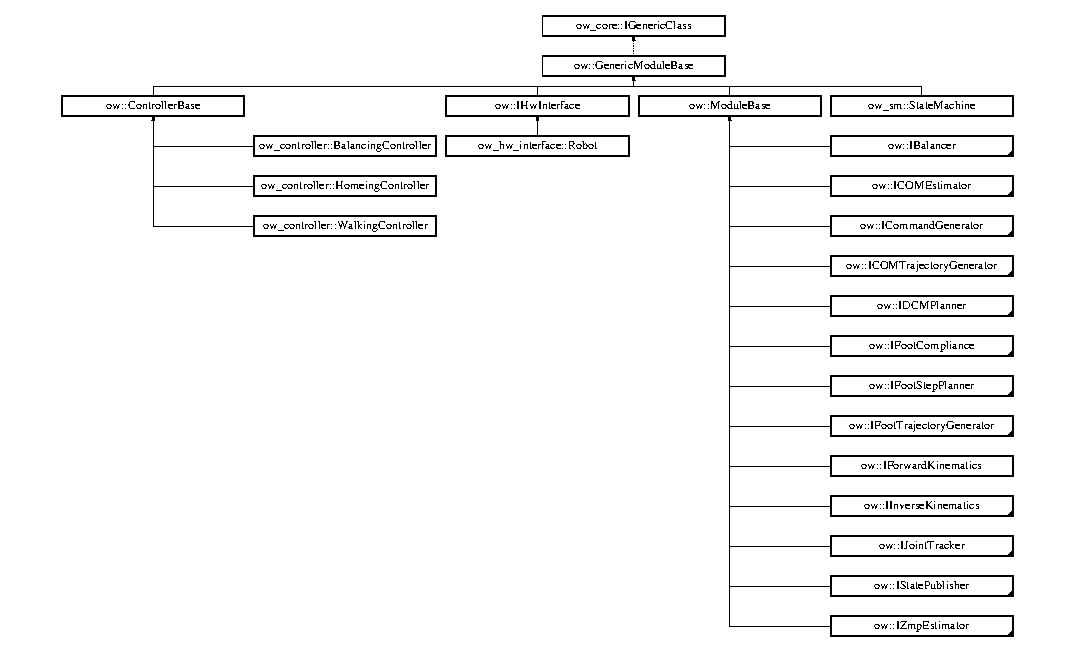
\includegraphics[height=8.334884cm]{db/dda/classow_1_1GenericModuleBase}
\end{center}
\end{figure}
\subsection*{Public Types}
\begin{DoxyCompactItemize}
\item 
enum \hyperlink{classow_1_1GenericModuleBase_a7886432615a5e12657f4a684607e6fdf}{State} \{ {\bfseries C\+O\+N\+S\+T\+R\+U\+C\+T\+ED}, 
{\bfseries I\+N\+I\+T\+I\+A\+L\+I\+Z\+ED}, 
{\bfseries R\+U\+N\+N\+I\+NG}
 \}\hypertarget{classow_1_1GenericModuleBase_a7886432615a5e12657f4a684607e6fdf}{}\label{classow_1_1GenericModuleBase_a7886432615a5e12657f4a684607e6fdf}
\begin{DoxyCompactList}\small\item\em Current state of the module. \end{DoxyCompactList}
\end{DoxyCompactItemize}
\subsection*{Public Member Functions}
\begin{DoxyCompactItemize}
\item 
\hyperlink{classow_1_1GenericModuleBase_acdbc9380752e797b3093d6f5fb506b76}{Generic\+Module\+Base} (const std\+::string \&\hyperlink{classow_1_1GenericModuleBase_a4b712883728cdbab7779e27f9a23689c}{name})\hypertarget{classow_1_1GenericModuleBase_acdbc9380752e797b3093d6f5fb506b76}{}\label{classow_1_1GenericModuleBase_acdbc9380752e797b3093d6f5fb506b76}

\begin{DoxyCompactList}\small\item\em Constructor. \end{DoxyCompactList}\item 
virtual \hyperlink{classow_1_1GenericModuleBase_a9bcecd007b2665363ab0e3e6ac03c60f}{$\sim$\+Generic\+Module\+Base} ()\hypertarget{classow_1_1GenericModuleBase_a9bcecd007b2665363ab0e3e6ac03c60f}{}\label{classow_1_1GenericModuleBase_a9bcecd007b2665363ab0e3e6ac03c60f}

\begin{DoxyCompactList}\small\item\em Virtual destructor. \end{DoxyCompactList}\item 
bool \hyperlink{classow_1_1GenericModuleBase_aef59a4b0b68ee9ba0b6cc9fe1ac910bd}{is\+Initialized} () const 
\begin{DoxyCompactList}\small\item\em return if is running \end{DoxyCompactList}\item 
bool \hyperlink{classow_1_1GenericModuleBase_a1450a5878a6791751434518e65be8665}{is\+Running} () const 
\begin{DoxyCompactList}\small\item\em return if is running \end{DoxyCompactList}\item 
std\+::string \hyperlink{classow_1_1GenericModuleBase_a4b712883728cdbab7779e27f9a23689c}{name} () const \hypertarget{classow_1_1GenericModuleBase_a4b712883728cdbab7779e27f9a23689c}{}\label{classow_1_1GenericModuleBase_a4b712883728cdbab7779e27f9a23689c}

\begin{DoxyCompactList}\small\item\em get state name \end{DoxyCompactList}\item 
std\+::string \hyperlink{classow_1_1GenericModuleBase_ac5d1344fc2d1ab4a67dffa262a48428a}{class\+Type} () const \hypertarget{classow_1_1GenericModuleBase_ac5d1344fc2d1ab4a67dffa262a48428a}{}\label{classow_1_1GenericModuleBase_ac5d1344fc2d1ab4a67dffa262a48428a}

\begin{DoxyCompactList}\small\item\em get state name \end{DoxyCompactList}\item 
ros\+::\+Time \hyperlink{classow_1_1GenericModuleBase_a5378be2f445ea95b0569926461775920}{start\+Time} () const \hypertarget{classow_1_1GenericModuleBase_a5378be2f445ea95b0569926461775920}{}\label{classow_1_1GenericModuleBase_a5378be2f445ea95b0569926461775920}

\begin{DoxyCompactList}\small\item\em get start time \end{DoxyCompactList}\item 
ros\+::\+Time \hyperlink{classow_1_1GenericModuleBase_a613e760af794382f43c0607a1891269f}{stop\+Time} () const \hypertarget{classow_1_1GenericModuleBase_a613e760af794382f43c0607a1891269f}{}\label{classow_1_1GenericModuleBase_a613e760af794382f43c0607a1891269f}

\begin{DoxyCompactList}\small\item\em get stop time \end{DoxyCompactList}\item 
bool \hyperlink{classow_1_1GenericModuleBase_ad3c3af233e4c726769bb3bdca14c3e10}{init\+Request} (const \hyperlink{classow_1_1Parameter}{ow\+::\+Parameter} \&parameter, ros\+::\+Node\+Handle \&nh)
\begin{DoxyCompactList}\small\item\em init interal \end{DoxyCompactList}\end{DoxyCompactItemize}
\subsection*{Protected Member Functions}
\begin{DoxyCompactItemize}
\item 
virtual bool \hyperlink{classow_1_1GenericModuleBase_a95c6c7b7a84acd2b4f37b7f9301abf9d}{init} (const \hyperlink{classow_1_1Parameter}{ow\+::\+Parameter} \&parameter, ros\+::\+Node\+Handle \&nh)=0
\begin{DoxyCompactList}\small\item\em init interal \end{DoxyCompactList}\item 
bool \hyperlink{classow_1_1GenericModuleBase_a30cd7aaffeaa38203ddb9c3366454458}{set\+Start\+State} (const ros\+::\+Time \&time)
\begin{DoxyCompactList}\small\item\em start the module \end{DoxyCompactList}\item 
bool \hyperlink{classow_1_1GenericModuleBase_a7a9a90a87f242094334e264429ab08ec}{set\+Stop\+State} (const ros\+::\+Time \&time)
\begin{DoxyCompactList}\small\item\em stop the module \end{DoxyCompactList}\end{DoxyCompactItemize}
\subsection*{Protected Attributes}
\begin{DoxyCompactItemize}
\item 
\hyperlink{classow_1_1GenericModuleBase_a7886432615a5e12657f4a684607e6fdf}{State} \hyperlink{classow_1_1GenericModuleBase_adc4bc6b792fa26a3cced4c4ceb64f72a}{state\+\_\+}\hypertarget{classow_1_1GenericModuleBase_adc4bc6b792fa26a3cced4c4ceb64f72a}{}\label{classow_1_1GenericModuleBase_adc4bc6b792fa26a3cced4c4ceb64f72a}

\begin{DoxyCompactList}\small\item\em the current module state \end{DoxyCompactList}\item 
std\+::string \hyperlink{classow_1_1GenericModuleBase_a576b6006ca06dc4b3c18d70c8ab3d2d4}{name\+\_\+}\hypertarget{classow_1_1GenericModuleBase_a576b6006ca06dc4b3c18d70c8ab3d2d4}{}\label{classow_1_1GenericModuleBase_a576b6006ca06dc4b3c18d70c8ab3d2d4}

\begin{DoxyCompactList}\small\item\em the module name \end{DoxyCompactList}\item 
ros\+::\+Time \hyperlink{classow_1_1GenericModuleBase_a5466cbf6c2258a91e2eb8d7bd9a0d29c}{start\+\_\+time\+\_\+}\hypertarget{classow_1_1GenericModuleBase_a5466cbf6c2258a91e2eb8d7bd9a0d29c}{}\label{classow_1_1GenericModuleBase_a5466cbf6c2258a91e2eb8d7bd9a0d29c}

\begin{DoxyCompactList}\small\item\em start time of the module \end{DoxyCompactList}\item 
ros\+::\+Time \hyperlink{classow_1_1GenericModuleBase_af1699d91f5cbb371dc4fe18b67bbd66e}{stop\+\_\+time\+\_\+}\hypertarget{classow_1_1GenericModuleBase_af1699d91f5cbb371dc4fe18b67bbd66e}{}\label{classow_1_1GenericModuleBase_af1699d91f5cbb371dc4fe18b67bbd66e}

\begin{DoxyCompactList}\small\item\em stop time of the module \end{DoxyCompactList}\end{DoxyCompactItemize}


\subsection{Detailed Description}
The \hyperlink{classow_1_1GenericModuleBase}{Generic\+Module\+Base} class. 

This provides the basic functionallity to initialize a module. Keeps track of module state. 

\subsection{Member Function Documentation}
\index{ow\+::\+Generic\+Module\+Base@{ow\+::\+Generic\+Module\+Base}!init@{init}}
\index{init@{init}!ow\+::\+Generic\+Module\+Base@{ow\+::\+Generic\+Module\+Base}}
\subsubsection[{\texorpdfstring{init(const ow\+::\+Parameter \&parameter, ros\+::\+Node\+Handle \&nh)=0}{init(const ow::Parameter &parameter, ros::NodeHandle &nh)=0}}]{\setlength{\rightskip}{0pt plus 5cm}virtual bool ow\+::\+Generic\+Module\+Base\+::init (
\begin{DoxyParamCaption}
\item[{const {\bf ow\+::\+Parameter} \&}]{parameter, }
\item[{ros\+::\+Node\+Handle \&}]{nh}
\end{DoxyParamCaption}
)\hspace{0.3cm}{\ttfamily [protected]}, {\ttfamily [pure virtual]}}\hypertarget{classow_1_1GenericModuleBase_a95c6c7b7a84acd2b4f37b7f9301abf9d}{}\label{classow_1_1GenericModuleBase_a95c6c7b7a84acd2b4f37b7f9301abf9d}


init interal 


\begin{DoxyParams}{Parameters}
{\em ros} & nh for namespace \\
\hline
\end{DoxyParams}


Implemented in \hyperlink{classow__fs__planner_1_1FootstepPlanner_ab3240b5742fb9188a5120c558db6c0bd}{ow\+\_\+fs\+\_\+planner\+::\+Footstep\+Planner}, \hyperlink{classow__pub_1_1StatePublisher_a3285df66b266dc6dd9468803f244f745}{ow\+\_\+pub\+::\+State\+Publisher}, \hyperlink{classow__sm_1_1StateMachine_a5bc07d8178b35935cc963a7015a30318}{ow\+\_\+sm\+::\+State\+Machine}, \hyperlink{classow__hw__interface_1_1Robot_ab4e66ad524fcce85b3c2a2a8dc375cc6}{ow\+\_\+hw\+\_\+interface\+::\+Robot}, \hyperlink{classow__joint__tracker_1_1JointTracker_a39a2e5dd308b1653205b255ecdd31ffb}{ow\+\_\+joint\+\_\+tracker\+::\+Joint\+Tracker}, \hyperlink{classow__zmp_1_1ZmpEstimator_a9e643e1ae0e0fedabbf753e42c0fd59b}{ow\+\_\+zmp\+::\+Zmp\+Estimator}, \hyperlink{classow__fcm_1_1FootCompliance_ad2459eb9b3936e928465a7a00dfb20c4}{ow\+\_\+fcm\+::\+Foot\+Compliance}, \hyperlink{classow__controller_1_1WalkingController_a0e9637665918f28e5e28b7ee24a119df}{ow\+\_\+controller\+::\+Walking\+Controller}, \hyperlink{classow__balancer_1_1Balancer_ab864c91d85ec802e833efcbabe41dec7}{ow\+\_\+balancer\+::\+Balancer}, \hyperlink{classow__controller_1_1BalancingController_a1b06a2454dd0ce27675390af723d2029}{ow\+\_\+controller\+::\+Balancing\+Controller}, \hyperlink{classow__cmd__gen_1_1CommandGenerator_ab36dd341b8d384aa134ed3ea8f4ae086}{ow\+\_\+cmd\+\_\+gen\+::\+Command\+Generator}, \hyperlink{classow__ftg_1_1FootTrajectoryGenerator_a76ea67492cbcedb85dce1ad5ec43699f}{ow\+\_\+ftg\+::\+Foot\+Trajectory\+Generator}, \hyperlink{classow__com__tg_1_1COMTrajectoryGenerator_ab0e21245b1f9f873a1df72969ed5e37d}{ow\+\_\+com\+\_\+tg\+::\+C\+O\+M\+Trajectory\+Generator}, \hyperlink{classow__dcm__planner_1_1DCMPlanner_ab846c11b13884d0f7ae1972de514b417}{ow\+\_\+dcm\+\_\+planner\+::\+D\+C\+M\+Planner}, \hyperlink{classow__ik_1_1InverseKinematics_a5469dd0c342af9bee2b5591d543540ec}{ow\+\_\+ik\+::\+Inverse\+Kinematics}, \hyperlink{classow__com_1_1COMEstimator_ac30dad4021919bc434ebb8a2b903163a}{ow\+\_\+com\+::\+C\+O\+M\+Estimator}, and \hyperlink{classow__controller_1_1HomeingController_aa9841489fbf7515ed7f26714eeba9f96}{ow\+\_\+controller\+::\+Homeing\+Controller}.

\index{ow\+::\+Generic\+Module\+Base@{ow\+::\+Generic\+Module\+Base}!init\+Request@{init\+Request}}
\index{init\+Request@{init\+Request}!ow\+::\+Generic\+Module\+Base@{ow\+::\+Generic\+Module\+Base}}
\subsubsection[{\texorpdfstring{init\+Request(const ow\+::\+Parameter \&parameter, ros\+::\+Node\+Handle \&nh)}{initRequest(const ow::Parameter &parameter, ros::NodeHandle &nh)}}]{\setlength{\rightskip}{0pt plus 5cm}bool ow\+::\+Generic\+Module\+Base\+::init\+Request (
\begin{DoxyParamCaption}
\item[{const {\bf ow\+::\+Parameter} \&}]{parameter, }
\item[{ros\+::\+Node\+Handle \&}]{nh}
\end{DoxyParamCaption}
)\hspace{0.3cm}{\ttfamily [inline]}}\hypertarget{classow_1_1GenericModuleBase_ad3c3af233e4c726769bb3bdca14c3e10}{}\label{classow_1_1GenericModuleBase_ad3c3af233e4c726769bb3bdca14c3e10}


init interal 


\begin{DoxyParams}{Parameters}
{\em ros} & nh for namespace \\
\hline
\end{DoxyParams}
\index{ow\+::\+Generic\+Module\+Base@{ow\+::\+Generic\+Module\+Base}!is\+Initialized@{is\+Initialized}}
\index{is\+Initialized@{is\+Initialized}!ow\+::\+Generic\+Module\+Base@{ow\+::\+Generic\+Module\+Base}}
\subsubsection[{\texorpdfstring{is\+Initialized() const }{isInitialized() const }}]{\setlength{\rightskip}{0pt plus 5cm}bool ow\+::\+Generic\+Module\+Base\+::is\+Initialized (
\begin{DoxyParamCaption}
{}
\end{DoxyParamCaption}
) const\hspace{0.3cm}{\ttfamily [inline]}}\hypertarget{classow_1_1GenericModuleBase_aef59a4b0b68ee9ba0b6cc9fe1ac910bd}{}\label{classow_1_1GenericModuleBase_aef59a4b0b68ee9ba0b6cc9fe1ac910bd}


return if is running 

\begin{DoxyReturn}{Returns}
running flag 
\end{DoxyReturn}
\index{ow\+::\+Generic\+Module\+Base@{ow\+::\+Generic\+Module\+Base}!is\+Running@{is\+Running}}
\index{is\+Running@{is\+Running}!ow\+::\+Generic\+Module\+Base@{ow\+::\+Generic\+Module\+Base}}
\subsubsection[{\texorpdfstring{is\+Running() const }{isRunning() const }}]{\setlength{\rightskip}{0pt plus 5cm}bool ow\+::\+Generic\+Module\+Base\+::is\+Running (
\begin{DoxyParamCaption}
{}
\end{DoxyParamCaption}
) const\hspace{0.3cm}{\ttfamily [inline]}}\hypertarget{classow_1_1GenericModuleBase_a1450a5878a6791751434518e65be8665}{}\label{classow_1_1GenericModuleBase_a1450a5878a6791751434518e65be8665}


return if is running 

\begin{DoxyReturn}{Returns}
running flag 
\end{DoxyReturn}
\index{ow\+::\+Generic\+Module\+Base@{ow\+::\+Generic\+Module\+Base}!set\+Start\+State@{set\+Start\+State}}
\index{set\+Start\+State@{set\+Start\+State}!ow\+::\+Generic\+Module\+Base@{ow\+::\+Generic\+Module\+Base}}
\subsubsection[{\texorpdfstring{set\+Start\+State(const ros\+::\+Time \&time)}{setStartState(const ros::Time &time)}}]{\setlength{\rightskip}{0pt plus 5cm}bool ow\+::\+Generic\+Module\+Base\+::set\+Start\+State (
\begin{DoxyParamCaption}
\item[{const ros\+::\+Time \&}]{time}
\end{DoxyParamCaption}
)\hspace{0.3cm}{\ttfamily [inline]}, {\ttfamily [protected]}}\hypertarget{classow_1_1GenericModuleBase_a30cd7aaffeaa38203ddb9c3366454458}{}\label{classow_1_1GenericModuleBase_a30cd7aaffeaa38203ddb9c3366454458}


start the module 


\begin{DoxyParams}{Parameters}
{\em starting} & time \\
\hline
\end{DoxyParams}
\index{ow\+::\+Generic\+Module\+Base@{ow\+::\+Generic\+Module\+Base}!set\+Stop\+State@{set\+Stop\+State}}
\index{set\+Stop\+State@{set\+Stop\+State}!ow\+::\+Generic\+Module\+Base@{ow\+::\+Generic\+Module\+Base}}
\subsubsection[{\texorpdfstring{set\+Stop\+State(const ros\+::\+Time \&time)}{setStopState(const ros::Time &time)}}]{\setlength{\rightskip}{0pt plus 5cm}bool ow\+::\+Generic\+Module\+Base\+::set\+Stop\+State (
\begin{DoxyParamCaption}
\item[{const ros\+::\+Time \&}]{time}
\end{DoxyParamCaption}
)\hspace{0.3cm}{\ttfamily [inline]}, {\ttfamily [protected]}}\hypertarget{classow_1_1GenericModuleBase_a7a9a90a87f242094334e264429ab08ec}{}\label{classow_1_1GenericModuleBase_a7a9a90a87f242094334e264429ab08ec}


stop the module 


\begin{DoxyParams}{Parameters}
{\em stopping} & time \\
\hline
\end{DoxyParams}


The documentation for this class was generated from the following file\+:\begin{DoxyCompactItemize}
\item 
/home/flo/work/ros/workspaces/ow\+\_\+ws/src/ow\+\_\+core/include/ow\+\_\+core/interfaces/\hyperlink{generic__module__base_8h}{generic\+\_\+module\+\_\+base.\+h}\end{DoxyCompactItemize}

\hypertarget{classow__controller_1_1HomeingController}{}\section{ow\+\_\+controller\+:\+:Homeing\+Controller Class Reference}
\label{classow__controller_1_1HomeingController}\index{ow\+\_\+controller\+::\+Homeing\+Controller@{ow\+\_\+controller\+::\+Homeing\+Controller}}


The \hyperlink{classow__controller_1_1HomeingController}{Homeing\+Controller} class.  




{\ttfamily \#include $<$homeing\+\_\+controller.\+h$>$}

Inheritance diagram for ow\+\_\+controller\+:\+:Homeing\+Controller\+:\begin{figure}[H]
\begin{center}
\leavevmode
\includegraphics[height=4.000000cm]{de/d6a/classow__controller_1_1HomeingController}
\end{center}
\end{figure}
\subsection*{Public Types}
\begin{DoxyCompactItemize}
\item 
typedef \hyperlink{classow_1_1ControllerBase}{ow\+::\+Controller\+Base} {\bfseries Base}\hypertarget{classow__controller_1_1HomeingController_a2fd2e36683df7e94da7b107f216a8f2b}{}\label{classow__controller_1_1HomeingController_a2fd2e36683df7e94da7b107f216a8f2b}

\end{DoxyCompactItemize}
\subsection*{Public Member Functions}
\begin{DoxyCompactItemize}
\item 
\hyperlink{classow__controller_1_1HomeingController_a21bed77590bf3c6998c2452e6869b3f6}{Homeing\+Controller} (const \hyperlink{classow_1_1IHwInterface}{ow\+::\+I\+Hw\+Interface} \&robot)
\begin{DoxyCompactList}\small\item\em Default constructor. \end{DoxyCompactList}\item 
virtual \hyperlink{classow__controller_1_1HomeingController_a690c588438cf3abd8c898fa7600113e7}{$\sim$\+Homeing\+Controller} ()\hypertarget{classow__controller_1_1HomeingController_a690c588438cf3abd8c898fa7600113e7}{}\label{classow__controller_1_1HomeingController_a690c588438cf3abd8c898fa7600113e7}

\begin{DoxyCompactList}\small\item\em Deconstructor. \end{DoxyCompactList}\item 
virtual bool \hyperlink{classow__controller_1_1HomeingController_aa9841489fbf7515ed7f26714eeba9f96}{init} (const \hyperlink{classow_1_1Parameter}{ow\+::\+Parameter} \&parameter, ros\+::\+Node\+Handle \&nh)
\begin{DoxyCompactList}\small\item\em init interal \end{DoxyCompactList}\item 
virtual void \hyperlink{classow__controller_1_1HomeingController_a7ef74fa759dd3ceab2913d31c42fa90e}{start} (const \hyperlink{classow_1_1IHwInterface}{ow\+::\+I\+Hw\+Interface} \&robot, const ros\+::\+Time \&time)
\begin{DoxyCompactList}\small\item\em start the controller, called befor update \end{DoxyCompactList}\item 
virtual \hyperlink{classow__core_1_1JointState}{ow\+::\+Joint\+State} \hyperlink{classow__controller_1_1HomeingController_ab703611f1f341457b3944a29c5a435d9}{update} (const \hyperlink{classow_1_1IHwInterface}{ow\+::\+I\+Hw\+Interface} \&robot, const ros\+::\+Time \&time, const ros\+::\+Duration \&dt)
\begin{DoxyCompactList}\small\item\em performs update step of the controller, called periodically \end{DoxyCompactList}\end{DoxyCompactItemize}
\subsection*{Protected Attributes}
\begin{DoxyCompactItemize}
\item 
\hyperlink{classow_1_1Parameter}{ow\+::\+Parameter} \hyperlink{classow__controller_1_1HomeingController_afaac4ec3eaa23b3d017f867dab5ce3af}{parameter\+\_\+}\hypertarget{classow__controller_1_1HomeingController_afaac4ec3eaa23b3d017f867dab5ce3af}{}\label{classow__controller_1_1HomeingController_afaac4ec3eaa23b3d017f867dab5ce3af}

\begin{DoxyCompactList}\small\item\em Configuration. \end{DoxyCompactList}\item 
\hyperlink{classow__core_1_1Flags}{ow\+\_\+core\+::\+Flags} \hyperlink{classow__controller_1_1HomeingController_ac73fe1fad1a9c7786b96e79319bab5cc}{flags\+\_\+}\hypertarget{classow__controller_1_1HomeingController_ac73fe1fad1a9c7786b96e79319bab5cc}{}\label{classow__controller_1_1HomeingController_ac73fe1fad1a9c7786b96e79319bab5cc}

\begin{DoxyCompactList}\small\item\em Walking flags. \end{DoxyCompactList}\item 
\hyperlink{classow__ik_1_1InverseKinematics}{ow\+\_\+ik\+::\+Inverse\+Kinematics} \hyperlink{classow__controller_1_1HomeingController_afb127afebd6bf06d43780ec9b37dfe3f}{ik\+\_\+}\hypertarget{classow__controller_1_1HomeingController_afb127afebd6bf06d43780ec9b37dfe3f}{}\label{classow__controller_1_1HomeingController_afb127afebd6bf06d43780ec9b37dfe3f}

\begin{DoxyCompactList}\small\item\em Inverse kinematics. \end{DoxyCompactList}\item 
\hyperlink{classow__joint__tracker_1_1JointTracker}{ow\+\_\+joint\+\_\+tracker\+::\+Joint\+Tracker} \hyperlink{classow__controller_1_1HomeingController_a542b7e41c2a2277476ace181003b0475}{joint\+\_\+tracker\+\_\+}\hypertarget{classow__controller_1_1HomeingController_a542b7e41c2a2277476ace181003b0475}{}\label{classow__controller_1_1HomeingController_a542b7e41c2a2277476ace181003b0475}

\begin{DoxyCompactList}\small\item\em Joint tracker. \end{DoxyCompactList}\item 
\hyperlink{classow__pub_1_1StatePublisher}{ow\+\_\+pub\+::\+State\+Publisher} \hyperlink{classow__controller_1_1HomeingController_ae3ce509f6041ba1f3dc07264c17e4daf}{pub\+\_\+}\hypertarget{classow__controller_1_1HomeingController_ae3ce509f6041ba1f3dc07264c17e4daf}{}\label{classow__controller_1_1HomeingController_ae3ce509f6041ba1f3dc07264c17e4daf}

\begin{DoxyCompactList}\small\item\em ros publisher \end{DoxyCompactList}\item 
std\+::vector$<$ \hyperlink{classow_1_1ModuleBase}{ow\+::\+Module\+Base} $\ast$ $>$ \hyperlink{classow__controller_1_1HomeingController_a5426446735fb0666146f5c86aa30afa9}{modules\+\_\+}\hypertarget{classow__controller_1_1HomeingController_a5426446735fb0666146f5c86aa30afa9}{}\label{classow__controller_1_1HomeingController_a5426446735fb0666146f5c86aa30afa9}

\begin{DoxyCompactList}\small\item\em vector of modules \end{DoxyCompactList}\item 
\hyperlink{classow__core_1_1JointPosition}{ow\+::\+Joint\+Position} \hyperlink{classow__controller_1_1HomeingController_a0c238940f782d6d2ec2334e1c8230d2f}{q\+\_\+fixed\+\_\+upper\+\_\+body\+\_\+}\hypertarget{classow__controller_1_1HomeingController_a0c238940f782d6d2ec2334e1c8230d2f}{}\label{classow__controller_1_1HomeingController_a0c238940f782d6d2ec2334e1c8230d2f}

\begin{DoxyCompactList}\small\item\em Upper body home posture. \end{DoxyCompactList}\item 
\hyperlink{classow__core_1_1JointState}{ow\+::\+Joint\+State} \hyperlink{classow__controller_1_1HomeingController_aa8810d39e4d4edaaba82df19abe87b93}{q\+\_\+}\hypertarget{classow__controller_1_1HomeingController_aa8810d39e4d4edaaba82df19abe87b93}{}\label{classow__controller_1_1HomeingController_aa8810d39e4d4edaaba82df19abe87b93}

\begin{DoxyCompactList}\small\item\em Output joint state. \end{DoxyCompactList}\item 
\hyperlink{classow__core_1_1CartesianState}{ow\+::\+Cartesian\+State} \hyperlink{classow__controller_1_1HomeingController_ad7fad20e1bf18a65547adc18e6adb247}{Xref\+\_\+l\+\_\+w\+\_\+}\hypertarget{classow__controller_1_1HomeingController_ad7fad20e1bf18a65547adc18e6adb247}{}\label{classow__controller_1_1HomeingController_ad7fad20e1bf18a65547adc18e6adb247}

\begin{DoxyCompactList}\small\item\em Reference left foot Cart state wrt world. \end{DoxyCompactList}\item 
\hyperlink{classow__core_1_1CartesianState}{ow\+::\+Cartesian\+State} \hyperlink{classow__controller_1_1HomeingController_a11a20d34fd3b1950b5505bad9924c76a}{Xref\+\_\+r\+\_\+w\+\_\+}\hypertarget{classow__controller_1_1HomeingController_a11a20d34fd3b1950b5505bad9924c76a}{}\label{classow__controller_1_1HomeingController_a11a20d34fd3b1950b5505bad9924c76a}

\begin{DoxyCompactList}\small\item\em Reference right foot Cart state wrt world. \end{DoxyCompactList}\item 
\hyperlink{classow__core_1_1CartesianState}{ow\+::\+Cartesian\+State} \hyperlink{classow__controller_1_1HomeingController_ac48d8776f0a2c8060bf186bf343860d2}{Xref\+\_\+com\+\_\+w\+\_\+}\hypertarget{classow__controller_1_1HomeingController_ac48d8776f0a2c8060bf186bf343860d2}{}\label{classow__controller_1_1HomeingController_ac48d8776f0a2c8060bf186bf343860d2}

\begin{DoxyCompactList}\small\item\em Reference CoM foot Cart state wrt world. \end{DoxyCompactList}\end{DoxyCompactItemize}
\subsection*{Additional Inherited Members}


\subsection{Detailed Description}
The \hyperlink{classow__controller_1_1HomeingController}{Homeing\+Controller} class. 

This Class uses some modules of the framework to execute the homing motion of the robot. It obtains the real robot data through the \hyperlink{classow_1_1IHwInterface}{ow\+::\+I\+Hw\+Interface} and calls the update functions on each module. Finally the \hyperlink{classow__controller_1_1HomeingController}{Homeing\+Controller} produces a new joint command that is then send to to the robot.

This controller can be enabled in the ow\+\_\+ros\+\_\+control\+\_\+plugin package. It is mainly used for debugging. 

\subsection{Constructor \& Destructor Documentation}
\index{ow\+\_\+controller\+::\+Homeing\+Controller@{ow\+\_\+controller\+::\+Homeing\+Controller}!Homeing\+Controller@{Homeing\+Controller}}
\index{Homeing\+Controller@{Homeing\+Controller}!ow\+\_\+controller\+::\+Homeing\+Controller@{ow\+\_\+controller\+::\+Homeing\+Controller}}
\subsubsection[{\texorpdfstring{Homeing\+Controller(const ow\+::\+I\+Hw\+Interface \&robot)}{HomeingController(const ow::IHwInterface &robot)}}]{\setlength{\rightskip}{0pt plus 5cm}ow\+\_\+controller\+::\+Homeing\+Controller\+::\+Homeing\+Controller (
\begin{DoxyParamCaption}
\item[{const {\bf ow\+::\+I\+Hw\+Interface} \&}]{robot}
\end{DoxyParamCaption}
)}\hypertarget{classow__controller_1_1HomeingController_a21bed77590bf3c6998c2452e6869b3f6}{}\label{classow__controller_1_1HomeingController_a21bed77590bf3c6998c2452e6869b3f6}


Default constructor. 


\begin{DoxyParams}{Parameters}
{\em freq} & \\
\hline
\end{DoxyParams}


\subsection{Member Function Documentation}
\index{ow\+\_\+controller\+::\+Homeing\+Controller@{ow\+\_\+controller\+::\+Homeing\+Controller}!init@{init}}
\index{init@{init}!ow\+\_\+controller\+::\+Homeing\+Controller@{ow\+\_\+controller\+::\+Homeing\+Controller}}
\subsubsection[{\texorpdfstring{init(const ow\+::\+Parameter \&parameter, ros\+::\+Node\+Handle \&nh)}{init(const ow::Parameter &parameter, ros::NodeHandle &nh)}}]{\setlength{\rightskip}{0pt plus 5cm}virtual bool ow\+\_\+controller\+::\+Homeing\+Controller\+::init (
\begin{DoxyParamCaption}
\item[{const {\bf ow\+::\+Parameter} \&}]{parameter, }
\item[{ros\+::\+Node\+Handle \&}]{nh}
\end{DoxyParamCaption}
)\hspace{0.3cm}{\ttfamily [virtual]}}\hypertarget{classow__controller_1_1HomeingController_aa9841489fbf7515ed7f26714eeba9f96}{}\label{classow__controller_1_1HomeingController_aa9841489fbf7515ed7f26714eeba9f96}


init interal 


\begin{DoxyParams}{Parameters}
{\em ros} & nh for namespace \\
\hline
\end{DoxyParams}


Implements \hyperlink{classow_1_1GenericModuleBase_a95c6c7b7a84acd2b4f37b7f9301abf9d}{ow\+::\+Generic\+Module\+Base}.

\index{ow\+\_\+controller\+::\+Homeing\+Controller@{ow\+\_\+controller\+::\+Homeing\+Controller}!start@{start}}
\index{start@{start}!ow\+\_\+controller\+::\+Homeing\+Controller@{ow\+\_\+controller\+::\+Homeing\+Controller}}
\subsubsection[{\texorpdfstring{start(const ow\+::\+I\+Hw\+Interface \&robot, const ros\+::\+Time \&time)}{start(const ow::IHwInterface &robot, const ros::Time &time)}}]{\setlength{\rightskip}{0pt plus 5cm}virtual void ow\+\_\+controller\+::\+Homeing\+Controller\+::start (
\begin{DoxyParamCaption}
\item[{const {\bf ow\+::\+I\+Hw\+Interface} \&}]{robot, }
\item[{const ros\+::\+Time \&}]{time}
\end{DoxyParamCaption}
)\hspace{0.3cm}{\ttfamily [virtual]}}\hypertarget{classow__controller_1_1HomeingController_a7ef74fa759dd3ceab2913d31c42fa90e}{}\label{classow__controller_1_1HomeingController_a7ef74fa759dd3ceab2913d31c42fa90e}


start the controller, called befor update 


\begin{DoxyParams}{Parameters}
{\em starting} & time \\
\hline
\end{DoxyParams}


Reimplemented from \hyperlink{classow_1_1ControllerBase_af757d63078346cff7888f3223d74da01}{ow\+::\+Controller\+Base}.

\index{ow\+\_\+controller\+::\+Homeing\+Controller@{ow\+\_\+controller\+::\+Homeing\+Controller}!update@{update}}
\index{update@{update}!ow\+\_\+controller\+::\+Homeing\+Controller@{ow\+\_\+controller\+::\+Homeing\+Controller}}
\subsubsection[{\texorpdfstring{update(const ow\+::\+I\+Hw\+Interface \&robot, const ros\+::\+Time \&time, const ros\+::\+Duration \&dt)}{update(const ow::IHwInterface &robot, const ros::Time &time, const ros::Duration &dt)}}]{\setlength{\rightskip}{0pt plus 5cm}virtual {\bf ow\+::\+Joint\+State} ow\+\_\+controller\+::\+Homeing\+Controller\+::update (
\begin{DoxyParamCaption}
\item[{const {\bf ow\+::\+I\+Hw\+Interface} \&}]{robot, }
\item[{const ros\+::\+Time \&}]{time, }
\item[{const ros\+::\+Duration \&}]{dt}
\end{DoxyParamCaption}
)\hspace{0.3cm}{\ttfamily [virtual]}}\hypertarget{classow__controller_1_1HomeingController_ab703611f1f341457b3944a29c5a435d9}{}\label{classow__controller_1_1HomeingController_ab703611f1f341457b3944a29c5a435d9}


performs update step of the controller, called periodically 


\begin{DoxyParams}{Parameters}
{\em current} & jointstate \\
\hline
{\em current} & time \\
\hline
{\em current} & deltatime since last call \\
\hline
\end{DoxyParams}


Implements \hyperlink{classow_1_1ControllerBase_a214e12fa933fd1dd3e720347e2757d2d}{ow\+::\+Controller\+Base}.



The documentation for this class was generated from the following file\+:\begin{DoxyCompactItemize}
\item 
/home/flo/work/ros/workspaces/ow\+\_\+ws/src/ow\+\_\+controller/include/ow\+\_\+controller/\hyperlink{homeing__controller_8h}{homeing\+\_\+controller.\+h}\end{DoxyCompactItemize}

\input{d5/de4/classow__core_1_1HomogeneousTransformation}
\hypertarget{classow_1_1IBalancer}{}\section{ow\+:\+:I\+Balancer Class Reference}
\label{classow_1_1IBalancer}\index{ow\+::\+I\+Balancer@{ow\+::\+I\+Balancer}}


The \hyperlink{classow_1_1IBalancer}{I\+Balancer} class.  




{\ttfamily \#include $<$i\+\_\+balancer.\+h$>$}

Inheritance diagram for ow\+:\+:I\+Balancer\+:\begin{figure}[H]
\begin{center}
\leavevmode
\includegraphics[height=5.000000cm]{d7/da1/classow_1_1IBalancer}
\end{center}
\end{figure}
\subsection*{Public Member Functions}
\begin{DoxyCompactItemize}
\item 
{\bfseries I\+Balancer} (const std\+::string \&\hyperlink{classow_1_1GenericModuleBase_a4b712883728cdbab7779e27f9a23689c}{name})\hypertarget{classow_1_1IBalancer_a1a0b556aaa2066e898ad6794aa810b4d}{}\label{classow_1_1IBalancer_a1a0b556aaa2066e898ad6794aa810b4d}

\item 
virtual \hyperlink{classow_1_1IBalancer_aa708682dd0caf0488bb7fd8e7b732c22}{$\sim$\+I\+Balancer} ()\hypertarget{classow_1_1IBalancer_aa708682dd0caf0488bb7fd8e7b732c22}{}\label{classow_1_1IBalancer_aa708682dd0caf0488bb7fd8e7b732c22}

\begin{DoxyCompactList}\small\item\em Virtual destructor. \end{DoxyCompactList}\item 
virtual const \hyperlink{classow__core_1_1CartesianState}{ow\+::\+Cartesian\+State} \& \hyperlink{classow_1_1IBalancer_a00656435faab973f7c5617aa3c318d51}{Xoff\+\_\+com} () const =0
\begin{DoxyCompactList}\small\item\em Output port function. \end{DoxyCompactList}\item 
virtual const \hyperlink{classow__core_1_1DivergentComponentOfMotionState}{ow\+::\+D\+C\+M\+State} \& \hyperlink{classow_1_1IBalancer_a4db08ea933f73841929abd5daba8be8f}{D\+C\+Md\+\_\+w} () const =0
\begin{DoxyCompactList}\small\item\em Output port function. \end{DoxyCompactList}\item 
virtual const \hyperlink{classow__core_1_1ZeroMomentPointState}{ow\+::\+Zero\+Moment\+Point\+State} \& \hyperlink{classow_1_1IBalancer_a7867ad2c24f117fa80d5cbf5074686ee}{Z\+M\+Pd\+\_\+w} () const =0
\begin{DoxyCompactList}\small\item\em Output port function. \end{DoxyCompactList}\end{DoxyCompactItemize}
\subsection*{Additional Inherited Members}


\subsection{Detailed Description}
The \hyperlink{classow_1_1IBalancer}{I\+Balancer} class. 

Interface class. 

\subsection{Member Function Documentation}
\index{ow\+::\+I\+Balancer@{ow\+::\+I\+Balancer}!D\+C\+Md\+\_\+w@{D\+C\+Md\+\_\+w}}
\index{D\+C\+Md\+\_\+w@{D\+C\+Md\+\_\+w}!ow\+::\+I\+Balancer@{ow\+::\+I\+Balancer}}
\subsubsection[{\texorpdfstring{D\+C\+Md\+\_\+w() const =0}{DCMd_w() const =0}}]{\setlength{\rightskip}{0pt plus 5cm}virtual const {\bf ow\+::\+D\+C\+M\+State}\& ow\+::\+I\+Balancer\+::\+D\+C\+Md\+\_\+w (
\begin{DoxyParamCaption}
{}
\end{DoxyParamCaption}
) const\hspace{0.3cm}{\ttfamily [pure virtual]}}\hypertarget{classow_1_1IBalancer_a4db08ea933f73841929abd5daba8be8f}{}\label{classow_1_1IBalancer_a4db08ea933f73841929abd5daba8be8f}


Output port function. 

\begin{DoxyReturn}{Returns}
D\+C\+M\+State of the desired Divergent Component Of Motion. 
\end{DoxyReturn}


Implemented in \hyperlink{classow__balancer_1_1Balancer_a09e9190ac09c6a4d1d1243f2db5bf8cb}{ow\+\_\+balancer\+::\+Balancer}.

\index{ow\+::\+I\+Balancer@{ow\+::\+I\+Balancer}!Xoff\+\_\+com@{Xoff\+\_\+com}}
\index{Xoff\+\_\+com@{Xoff\+\_\+com}!ow\+::\+I\+Balancer@{ow\+::\+I\+Balancer}}
\subsubsection[{\texorpdfstring{Xoff\+\_\+com() const =0}{Xoff_com() const =0}}]{\setlength{\rightskip}{0pt plus 5cm}virtual const {\bf ow\+::\+Cartesian\+State}\& ow\+::\+I\+Balancer\+::\+Xoff\+\_\+com (
\begin{DoxyParamCaption}
{}
\end{DoxyParamCaption}
) const\hspace{0.3cm}{\ttfamily [pure virtual]}}\hypertarget{classow_1_1IBalancer_a00656435faab973f7c5617aa3c318d51}{}\label{classow_1_1IBalancer_a00656435faab973f7c5617aa3c318d51}


Output port function. 

\begin{DoxyReturn}{Returns}
Cartesian\+State offset on the C\+OM commanded position to keep balance and track the reference trajectory. 
\end{DoxyReturn}


Implemented in \hyperlink{classow__balancer_1_1Balancer_a75e68c66c09e370b4b670ed7fcdafcd6}{ow\+\_\+balancer\+::\+Balancer}.

\index{ow\+::\+I\+Balancer@{ow\+::\+I\+Balancer}!Z\+M\+Pd\+\_\+w@{Z\+M\+Pd\+\_\+w}}
\index{Z\+M\+Pd\+\_\+w@{Z\+M\+Pd\+\_\+w}!ow\+::\+I\+Balancer@{ow\+::\+I\+Balancer}}
\subsubsection[{\texorpdfstring{Z\+M\+Pd\+\_\+w() const =0}{ZMPd_w() const =0}}]{\setlength{\rightskip}{0pt plus 5cm}virtual const {\bf ow\+::\+Zero\+Moment\+Point\+State}\& ow\+::\+I\+Balancer\+::\+Z\+M\+Pd\+\_\+w (
\begin{DoxyParamCaption}
{}
\end{DoxyParamCaption}
) const\hspace{0.3cm}{\ttfamily [pure virtual]}}\hypertarget{classow_1_1IBalancer_a7867ad2c24f117fa80d5cbf5074686ee}{}\label{classow_1_1IBalancer_a7867ad2c24f117fa80d5cbf5074686ee}


Output port function. 

\begin{DoxyReturn}{Returns}
Zero\+Moment\+Point\+State to keep balance and track the desired D\+CM. 
\end{DoxyReturn}


Implemented in \hyperlink{classow__balancer_1_1Balancer_a49b1432ce68fbb056a5c9426c11c7122}{ow\+\_\+balancer\+::\+Balancer}.



The documentation for this class was generated from the following file\+:\begin{DoxyCompactItemize}
\item 
/home/flo/work/ros/workspaces/ow\+\_\+ws/src/ow\+\_\+core/include/ow\+\_\+core/interfaces/\hyperlink{i__balancer_8h}{i\+\_\+balancer.\+h}\end{DoxyCompactItemize}

\hypertarget{classow_1_1ICOMEstimator}{}\section{ow\+:\+:I\+C\+O\+M\+Estimator Class Reference}
\label{classow_1_1ICOMEstimator}\index{ow\+::\+I\+C\+O\+M\+Estimator@{ow\+::\+I\+C\+O\+M\+Estimator}}


The \hyperlink{classow_1_1ICOMEstimator}{I\+C\+O\+M\+Estimator} class.  




{\ttfamily \#include $<$i\+\_\+com\+\_\+estimator.\+h$>$}

Inheritance diagram for ow\+:\+:I\+C\+O\+M\+Estimator\+:\begin{figure}[H]
\begin{center}
\leavevmode
\includegraphics[height=5.000000cm]{de/d6a/classow_1_1ICOMEstimator}
\end{center}
\end{figure}
\subsection*{Public Member Functions}
\begin{DoxyCompactItemize}
\item 
{\bfseries I\+C\+O\+M\+Estimator} (const std\+::string \&\hyperlink{classow_1_1GenericModuleBase_a4b712883728cdbab7779e27f9a23689c}{name})\hypertarget{classow_1_1ICOMEstimator_a602fce5de417ba1f245c7a6ee47b93d2}{}\label{classow_1_1ICOMEstimator_a602fce5de417ba1f245c7a6ee47b93d2}

\item 
virtual \hyperlink{classow_1_1ICOMEstimator_a9c1d13779ec3a3248cce49743f939302}{$\sim$\+I\+C\+O\+M\+Estimator} ()\hypertarget{classow_1_1ICOMEstimator_a9c1d13779ec3a3248cce49743f939302}{}\label{classow_1_1ICOMEstimator_a9c1d13779ec3a3248cce49743f939302}

\begin{DoxyCompactList}\small\item\em Virtual destructor. \end{DoxyCompactList}\item 
virtual const \hyperlink{classow__core_1_1CartesianState}{ow\+::\+Cartesian\+State} \& \hyperlink{classow_1_1ICOMEstimator_a96fc5dc80ed0f61b0a7a300d8519a9af}{Xf\+\_\+com\+\_\+w} () const =0
\begin{DoxyCompactList}\small\item\em Output port function. \end{DoxyCompactList}\item 
virtual const \hyperlink{classow__core_1_1DivergentComponentOfMotionState}{ow\+::\+D\+C\+M\+State} \& \hyperlink{classow_1_1ICOMEstimator_a39feef3509fbe0f8dbf358c28b067e43}{D\+C\+Mr\+\_\+w} () const =0
\begin{DoxyCompactList}\small\item\em Output port function. \end{DoxyCompactList}\end{DoxyCompactItemize}
\subsection*{Additional Inherited Members}


\subsection{Detailed Description}
The \hyperlink{classow_1_1ICOMEstimator}{I\+C\+O\+M\+Estimator} class. 

Interface class. 

\subsection{Member Function Documentation}
\index{ow\+::\+I\+C\+O\+M\+Estimator@{ow\+::\+I\+C\+O\+M\+Estimator}!D\+C\+Mr\+\_\+w@{D\+C\+Mr\+\_\+w}}
\index{D\+C\+Mr\+\_\+w@{D\+C\+Mr\+\_\+w}!ow\+::\+I\+C\+O\+M\+Estimator@{ow\+::\+I\+C\+O\+M\+Estimator}}
\subsubsection[{\texorpdfstring{D\+C\+Mr\+\_\+w() const =0}{DCMr_w() const =0}}]{\setlength{\rightskip}{0pt plus 5cm}virtual const {\bf ow\+::\+D\+C\+M\+State}\& ow\+::\+I\+C\+O\+M\+Estimator\+::\+D\+C\+Mr\+\_\+w (
\begin{DoxyParamCaption}
{}
\end{DoxyParamCaption}
) const\hspace{0.3cm}{\ttfamily [pure virtual]}}\hypertarget{classow_1_1ICOMEstimator_a39feef3509fbe0f8dbf358c28b067e43}{}\label{classow_1_1ICOMEstimator_a39feef3509fbe0f8dbf358c28b067e43}


Output port function. 

\begin{DoxyReturn}{Returns}
D\+C\+M\+State of the real robot 
\end{DoxyReturn}


Implemented in \hyperlink{classow__com_1_1COMEstimator_a70d5e11ea25009c7894d64763f72f26c}{ow\+\_\+com\+::\+C\+O\+M\+Estimator}.

\index{ow\+::\+I\+C\+O\+M\+Estimator@{ow\+::\+I\+C\+O\+M\+Estimator}!Xf\+\_\+com\+\_\+w@{Xf\+\_\+com\+\_\+w}}
\index{Xf\+\_\+com\+\_\+w@{Xf\+\_\+com\+\_\+w}!ow\+::\+I\+C\+O\+M\+Estimator@{ow\+::\+I\+C\+O\+M\+Estimator}}
\subsubsection[{\texorpdfstring{Xf\+\_\+com\+\_\+w() const =0}{Xf_com_w() const =0}}]{\setlength{\rightskip}{0pt plus 5cm}virtual const {\bf ow\+::\+Cartesian\+State}\& ow\+::\+I\+C\+O\+M\+Estimator\+::\+Xf\+\_\+com\+\_\+w (
\begin{DoxyParamCaption}
{}
\end{DoxyParamCaption}
) const\hspace{0.3cm}{\ttfamily [pure virtual]}}\hypertarget{classow_1_1ICOMEstimator_a96fc5dc80ed0f61b0a7a300d8519a9af}{}\label{classow_1_1ICOMEstimator_a96fc5dc80ed0f61b0a7a300d8519a9af}


Output port function. 

\begin{DoxyReturn}{Returns}
Cartesian\+State for the filtered pose of the real CoM. 
\end{DoxyReturn}


Implemented in \hyperlink{classow__com_1_1COMEstimator_af0474ec2ab3a61d06ab3dd80c70b0b2e}{ow\+\_\+com\+::\+C\+O\+M\+Estimator}.



The documentation for this class was generated from the following file\+:\begin{DoxyCompactItemize}
\item 
/home/flo/work/ros/workspaces/ow\+\_\+ws/src/ow\+\_\+core/include/ow\+\_\+core/interfaces/\hyperlink{i__com__estimator_8h}{i\+\_\+com\+\_\+estimator.\+h}\end{DoxyCompactItemize}

\hypertarget{classow_1_1ICommandGenerator}{}\section{ow\+:\+:I\+Command\+Generator Class Reference}
\label{classow_1_1ICommandGenerator}\index{ow\+::\+I\+Command\+Generator@{ow\+::\+I\+Command\+Generator}}


The \hyperlink{classow_1_1ICommandGenerator}{I\+Command\+Generator} class.  




{\ttfamily \#include $<$i\+\_\+command\+\_\+generator.\+h$>$}

Inheritance diagram for ow\+:\+:I\+Command\+Generator\+:\begin{figure}[H]
\begin{center}
\leavevmode
\includegraphics[height=5.000000cm]{df/d70/classow_1_1ICommandGenerator}
\end{center}
\end{figure}
\subsection*{Public Member Functions}
\begin{DoxyCompactItemize}
\item 
{\bfseries I\+Command\+Generator} (const std\+::string \&\hyperlink{classow_1_1GenericModuleBase_a4b712883728cdbab7779e27f9a23689c}{name})\hypertarget{classow_1_1ICommandGenerator_a2d1c06ce50f393fc2f2412341828da6e}{}\label{classow_1_1ICommandGenerator_a2d1c06ce50f393fc2f2412341828da6e}

\item 
virtual \hyperlink{classow_1_1ICommandGenerator_a3fa95de2b030993df8204013ec7bc039}{$\sim$\+I\+Command\+Generator} ()\hypertarget{classow_1_1ICommandGenerator_a3fa95de2b030993df8204013ec7bc039}{}\label{classow_1_1ICommandGenerator_a3fa95de2b030993df8204013ec7bc039}

\begin{DoxyCompactList}\small\item\em Virtual destructor. \end{DoxyCompactList}\item 
virtual const \hyperlink{classow__core_1_1CartesianState}{ow\+::\+Cartesian\+State} \& \hyperlink{classow_1_1ICommandGenerator_a964c3ff445e3de3aa19fb617b221b5b8}{Xcmd\+\_\+l\+\_\+w} () const =0
\begin{DoxyCompactList}\small\item\em Output port function. \end{DoxyCompactList}\item 
virtual const \hyperlink{classow__core_1_1CartesianState}{ow\+::\+Cartesian\+State} \& \hyperlink{classow_1_1ICommandGenerator_ae7309a2b5839ee3376380693617a0cdd}{Xcmd\+\_\+r\+\_\+w} () const =0
\begin{DoxyCompactList}\small\item\em Output port function. \end{DoxyCompactList}\item 
virtual const \hyperlink{classow__core_1_1CartesianState}{ow\+::\+Cartesian\+State} \& \hyperlink{classow_1_1ICommandGenerator_a3b635bf72503ad1e11d5edc8514a6ec0}{Xcmd\+\_\+com\+\_\+w} () const =0
\begin{DoxyCompactList}\small\item\em Output port function. \end{DoxyCompactList}\end{DoxyCompactItemize}
\subsection*{Additional Inherited Members}


\subsection{Detailed Description}
The \hyperlink{classow_1_1ICommandGenerator}{I\+Command\+Generator} class. 

Interface class. 

\subsection{Member Function Documentation}
\index{ow\+::\+I\+Command\+Generator@{ow\+::\+I\+Command\+Generator}!Xcmd\+\_\+com\+\_\+w@{Xcmd\+\_\+com\+\_\+w}}
\index{Xcmd\+\_\+com\+\_\+w@{Xcmd\+\_\+com\+\_\+w}!ow\+::\+I\+Command\+Generator@{ow\+::\+I\+Command\+Generator}}
\subsubsection[{\texorpdfstring{Xcmd\+\_\+com\+\_\+w() const =0}{Xcmd_com_w() const =0}}]{\setlength{\rightskip}{0pt plus 5cm}virtual const {\bf ow\+::\+Cartesian\+State}\& ow\+::\+I\+Command\+Generator\+::\+Xcmd\+\_\+com\+\_\+w (
\begin{DoxyParamCaption}
{}
\end{DoxyParamCaption}
) const\hspace{0.3cm}{\ttfamily [pure virtual]}}\hypertarget{classow_1_1ICommandGenerator_a3b635bf72503ad1e11d5edc8514a6ec0}{}\label{classow_1_1ICommandGenerator_a3b635bf72503ad1e11d5edc8514a6ec0}


Output port function. 

\begin{DoxyReturn}{Returns}
Cartesian\+State contains the commanded pose of the center of mass coordinate frame C\+OM with respect to the world coordinate frame W. 
\end{DoxyReturn}


Implemented in \hyperlink{classow__cmd__gen_1_1CommandGenerator_a104f8f57b30db712328970907f269f69}{ow\+\_\+cmd\+\_\+gen\+::\+Command\+Generator}.

\index{ow\+::\+I\+Command\+Generator@{ow\+::\+I\+Command\+Generator}!Xcmd\+\_\+l\+\_\+w@{Xcmd\+\_\+l\+\_\+w}}
\index{Xcmd\+\_\+l\+\_\+w@{Xcmd\+\_\+l\+\_\+w}!ow\+::\+I\+Command\+Generator@{ow\+::\+I\+Command\+Generator}}
\subsubsection[{\texorpdfstring{Xcmd\+\_\+l\+\_\+w() const =0}{Xcmd_l_w() const =0}}]{\setlength{\rightskip}{0pt plus 5cm}virtual const {\bf ow\+::\+Cartesian\+State}\& ow\+::\+I\+Command\+Generator\+::\+Xcmd\+\_\+l\+\_\+w (
\begin{DoxyParamCaption}
{}
\end{DoxyParamCaption}
) const\hspace{0.3cm}{\ttfamily [pure virtual]}}\hypertarget{classow_1_1ICommandGenerator_a964c3ff445e3de3aa19fb617b221b5b8}{}\label{classow_1_1ICommandGenerator_a964c3ff445e3de3aa19fb617b221b5b8}


Output port function. 

\begin{DoxyReturn}{Returns}
Cartesian\+State contains the commanded pose of the left foot ankle coordinate frame L with respect to the world coordinate frame W. 
\end{DoxyReturn}


Implemented in \hyperlink{classow__cmd__gen_1_1CommandGenerator_a922b9defd16847ef9cba70ed56c6019e}{ow\+\_\+cmd\+\_\+gen\+::\+Command\+Generator}.

\index{ow\+::\+I\+Command\+Generator@{ow\+::\+I\+Command\+Generator}!Xcmd\+\_\+r\+\_\+w@{Xcmd\+\_\+r\+\_\+w}}
\index{Xcmd\+\_\+r\+\_\+w@{Xcmd\+\_\+r\+\_\+w}!ow\+::\+I\+Command\+Generator@{ow\+::\+I\+Command\+Generator}}
\subsubsection[{\texorpdfstring{Xcmd\+\_\+r\+\_\+w() const =0}{Xcmd_r_w() const =0}}]{\setlength{\rightskip}{0pt plus 5cm}virtual const {\bf ow\+::\+Cartesian\+State}\& ow\+::\+I\+Command\+Generator\+::\+Xcmd\+\_\+r\+\_\+w (
\begin{DoxyParamCaption}
{}
\end{DoxyParamCaption}
) const\hspace{0.3cm}{\ttfamily [pure virtual]}}\hypertarget{classow_1_1ICommandGenerator_ae7309a2b5839ee3376380693617a0cdd}{}\label{classow_1_1ICommandGenerator_ae7309a2b5839ee3376380693617a0cdd}


Output port function. 

\begin{DoxyReturn}{Returns}
Cartesian\+State contains the commanded pose of the right foot ankle coordinate frame R with respect to the world coordinate frame W. 
\end{DoxyReturn}


Implemented in \hyperlink{classow__cmd__gen_1_1CommandGenerator_afd5c10bd19ed610f63c73a5516961584}{ow\+\_\+cmd\+\_\+gen\+::\+Command\+Generator}.



The documentation for this class was generated from the following file\+:\begin{DoxyCompactItemize}
\item 
/home/flo/work/ros/workspaces/ow\+\_\+ws/src/ow\+\_\+core/include/ow\+\_\+core/interfaces/\hyperlink{i__command__generator_8h}{i\+\_\+command\+\_\+generator.\+h}\end{DoxyCompactItemize}

\hypertarget{classow_1_1ICOMTrajectoryGenerator}{}\section{ow\+:\+:I\+C\+O\+M\+Trajectory\+Generator Class Reference}
\label{classow_1_1ICOMTrajectoryGenerator}\index{ow\+::\+I\+C\+O\+M\+Trajectory\+Generator@{ow\+::\+I\+C\+O\+M\+Trajectory\+Generator}}


The \hyperlink{classow_1_1ICOMTrajectoryGenerator}{I\+C\+O\+M\+Trajectory\+Generator} class.  




{\ttfamily \#include $<$i\+\_\+com\+\_\+trajectory\+\_\+generator.\+h$>$}

Inheritance diagram for ow\+:\+:I\+C\+O\+M\+Trajectory\+Generator\+:\begin{figure}[H]
\begin{center}
\leavevmode
\includegraphics[height=5.000000cm]{d3/d6d/classow_1_1ICOMTrajectoryGenerator}
\end{center}
\end{figure}
\subsection*{Public Member Functions}
\begin{DoxyCompactItemize}
\item 
{\bfseries I\+C\+O\+M\+Trajectory\+Generator} (const std\+::string \&\hyperlink{classow_1_1GenericModuleBase_a4b712883728cdbab7779e27f9a23689c}{name})\hypertarget{classow_1_1ICOMTrajectoryGenerator_a2fc5361a08d6d2e27f04a3539ed68965}{}\label{classow_1_1ICOMTrajectoryGenerator_a2fc5361a08d6d2e27f04a3539ed68965}

\item 
virtual \hyperlink{classow_1_1ICOMTrajectoryGenerator_ac018f29d8a184fe06903dc8a220b416c}{$\sim$\+I\+C\+O\+M\+Trajectory\+Generator} ()\hypertarget{classow_1_1ICOMTrajectoryGenerator_ac018f29d8a184fe06903dc8a220b416c}{}\label{classow_1_1ICOMTrajectoryGenerator_ac018f29d8a184fe06903dc8a220b416c}

\begin{DoxyCompactList}\small\item\em Virtual destructor. \end{DoxyCompactList}\item 
virtual const \hyperlink{classow__core_1_1ZeroMomentPointState}{ow\+::\+Zero\+Moment\+Point\+State} \& \hyperlink{classow_1_1ICOMTrajectoryGenerator_a45f42b461f2377055071338ef719aa50}{Z\+M\+P\+\_\+w} () const =0
\begin{DoxyCompactList}\small\item\em Output port function. \end{DoxyCompactList}\item 
virtual const \hyperlink{classow__core_1_1DivergentComponentOfMotionState}{ow\+::\+D\+C\+M\+State} \& \hyperlink{classow_1_1ICOMTrajectoryGenerator_aaca7b9f4233b9e2e44a586af52e9305d}{D\+C\+M\+\_\+w} () const =0
\begin{DoxyCompactList}\small\item\em Output port function. \end{DoxyCompactList}\item 
virtual const \hyperlink{classow__core_1_1CartesianState}{ow\+::\+Cartesian\+State} \& \hyperlink{classow_1_1ICOMTrajectoryGenerator_aa48c8eb75d6a9ff8752deb2df6aecb01}{X\+\_\+com\+\_\+w} () const =0
\begin{DoxyCompactList}\small\item\em Output port function. \end{DoxyCompactList}\end{DoxyCompactItemize}
\subsection*{Additional Inherited Members}


\subsection{Detailed Description}
The \hyperlink{classow_1_1ICOMTrajectoryGenerator}{I\+C\+O\+M\+Trajectory\+Generator} class. 

Interface class. 

\subsection{Member Function Documentation}
\index{ow\+::\+I\+C\+O\+M\+Trajectory\+Generator@{ow\+::\+I\+C\+O\+M\+Trajectory\+Generator}!D\+C\+M\+\_\+w@{D\+C\+M\+\_\+w}}
\index{D\+C\+M\+\_\+w@{D\+C\+M\+\_\+w}!ow\+::\+I\+C\+O\+M\+Trajectory\+Generator@{ow\+::\+I\+C\+O\+M\+Trajectory\+Generator}}
\subsubsection[{\texorpdfstring{D\+C\+M\+\_\+w() const =0}{DCM_w() const =0}}]{\setlength{\rightskip}{0pt plus 5cm}virtual const {\bf ow\+::\+D\+C\+M\+State}\& ow\+::\+I\+C\+O\+M\+Trajectory\+Generator\+::\+D\+C\+M\+\_\+w (
\begin{DoxyParamCaption}
{}
\end{DoxyParamCaption}
) const\hspace{0.3cm}{\ttfamily [pure virtual]}}\hypertarget{classow_1_1ICOMTrajectoryGenerator_aaca7b9f4233b9e2e44a586af52e9305d}{}\label{classow_1_1ICOMTrajectoryGenerator_aaca7b9f4233b9e2e44a586af52e9305d}


Output port function. 

\begin{DoxyReturn}{Returns}
Cartesian\+State of the Reference trajectory for the D\+CM. 
\end{DoxyReturn}


Implemented in \hyperlink{classow__com__tg_1_1COMTrajectoryGenerator_a611454aadb3bc551ee85753e8135233a}{ow\+\_\+com\+\_\+tg\+::\+C\+O\+M\+Trajectory\+Generator}.

\index{ow\+::\+I\+C\+O\+M\+Trajectory\+Generator@{ow\+::\+I\+C\+O\+M\+Trajectory\+Generator}!X\+\_\+com\+\_\+w@{X\+\_\+com\+\_\+w}}
\index{X\+\_\+com\+\_\+w@{X\+\_\+com\+\_\+w}!ow\+::\+I\+C\+O\+M\+Trajectory\+Generator@{ow\+::\+I\+C\+O\+M\+Trajectory\+Generator}}
\subsubsection[{\texorpdfstring{X\+\_\+com\+\_\+w() const =0}{X_com_w() const =0}}]{\setlength{\rightskip}{0pt plus 5cm}virtual const {\bf ow\+::\+Cartesian\+State}\& ow\+::\+I\+C\+O\+M\+Trajectory\+Generator\+::\+X\+\_\+com\+\_\+w (
\begin{DoxyParamCaption}
{}
\end{DoxyParamCaption}
) const\hspace{0.3cm}{\ttfamily [pure virtual]}}\hypertarget{classow_1_1ICOMTrajectoryGenerator_aa48c8eb75d6a9ff8752deb2df6aecb01}{}\label{classow_1_1ICOMTrajectoryGenerator_aa48c8eb75d6a9ff8752deb2df6aecb01}


Output port function. 

\begin{DoxyReturn}{Returns}
Cartesian\+State of the Reference trajectory for the CoM. This includes both po-\/sition and orientation of a virtual link located at the Co\+Mwith the same oriantation of the base link. 
\end{DoxyReturn}


Implemented in \hyperlink{classow__com__tg_1_1COMTrajectoryGenerator_af52006557c655237b92f85dcf10b8b9b}{ow\+\_\+com\+\_\+tg\+::\+C\+O\+M\+Trajectory\+Generator}.

\index{ow\+::\+I\+C\+O\+M\+Trajectory\+Generator@{ow\+::\+I\+C\+O\+M\+Trajectory\+Generator}!Z\+M\+P\+\_\+w@{Z\+M\+P\+\_\+w}}
\index{Z\+M\+P\+\_\+w@{Z\+M\+P\+\_\+w}!ow\+::\+I\+C\+O\+M\+Trajectory\+Generator@{ow\+::\+I\+C\+O\+M\+Trajectory\+Generator}}
\subsubsection[{\texorpdfstring{Z\+M\+P\+\_\+w() const =0}{ZMP_w() const =0}}]{\setlength{\rightskip}{0pt plus 5cm}virtual const {\bf ow\+::\+Zero\+Moment\+Point\+State}\& ow\+::\+I\+C\+O\+M\+Trajectory\+Generator\+::\+Z\+M\+P\+\_\+w (
\begin{DoxyParamCaption}
{}
\end{DoxyParamCaption}
) const\hspace{0.3cm}{\ttfamily [pure virtual]}}\hypertarget{classow_1_1ICOMTrajectoryGenerator_a45f42b461f2377055071338ef719aa50}{}\label{classow_1_1ICOMTrajectoryGenerator_a45f42b461f2377055071338ef719aa50}


Output port function. 

\begin{DoxyReturn}{Returns}
Cartesian\+State of the Reference trajectory for the Z\+MP. 
\end{DoxyReturn}


Implemented in \hyperlink{classow__com__tg_1_1COMTrajectoryGenerator_acec7a01af30b57cd99962a3e5d7bdf4f}{ow\+\_\+com\+\_\+tg\+::\+C\+O\+M\+Trajectory\+Generator}.



The documentation for this class was generated from the following file\+:\begin{DoxyCompactItemize}
\item 
/home/flo/work/ros/workspaces/ow\+\_\+ws/src/ow\+\_\+core/include/ow\+\_\+core/interfaces/\hyperlink{i__com__trajectory__generator_8h}{i\+\_\+com\+\_\+trajectory\+\_\+generator.\+h}\end{DoxyCompactItemize}

\hypertarget{classow_1_1IDCMPlanner}{}\section{ow\+:\+:I\+D\+C\+M\+Planner Class Reference}
\label{classow_1_1IDCMPlanner}\index{ow\+::\+I\+D\+C\+M\+Planner@{ow\+::\+I\+D\+C\+M\+Planner}}


The \hyperlink{classow_1_1IDCMPlanner}{I\+D\+C\+M\+Planner} class.  




{\ttfamily \#include $<$i\+\_\+dcm\+\_\+planner.\+h$>$}

Inheritance diagram for ow\+:\+:I\+D\+C\+M\+Planner\+:\begin{figure}[H]
\begin{center}
\leavevmode
\includegraphics[height=5.000000cm]{dd/da1/classow_1_1IDCMPlanner}
\end{center}
\end{figure}
\subsection*{Public Member Functions}
\begin{DoxyCompactItemize}
\item 
{\bfseries I\+D\+C\+M\+Planner} (const std\+::string \&\hyperlink{classow_1_1GenericModuleBase_a4b712883728cdbab7779e27f9a23689c}{name})\hypertarget{classow_1_1IDCMPlanner_a53d723c86945798888fa5d68cfa9dcfd}{}\label{classow_1_1IDCMPlanner_a53d723c86945798888fa5d68cfa9dcfd}

\item 
virtual \hyperlink{classow_1_1IDCMPlanner_a44f18545ecad2030712d21e5523d6bf1}{$\sim$\+I\+D\+C\+M\+Planner} ()\hypertarget{classow_1_1IDCMPlanner_a44f18545ecad2030712d21e5523d6bf1}{}\label{classow_1_1IDCMPlanner_a44f18545ecad2030712d21e5523d6bf1}

\begin{DoxyCompactList}\small\item\em Virtual destructor. \end{DoxyCompactList}\item 
virtual const ow\+::\+D\+C\+M\+Point\+Set\+List \& \hyperlink{classow_1_1IDCMPlanner_addf85aab043e49379fbe76c17ddae3c2}{dcm\+Point\+Set\+List} () const =0
\begin{DoxyCompactList}\small\item\em Output port function. \end{DoxyCompactList}\end{DoxyCompactItemize}
\subsection*{Additional Inherited Members}


\subsection{Detailed Description}
The \hyperlink{classow_1_1IDCMPlanner}{I\+D\+C\+M\+Planner} class. 

Interface class. 

\subsection{Member Function Documentation}
\index{ow\+::\+I\+D\+C\+M\+Planner@{ow\+::\+I\+D\+C\+M\+Planner}!dcm\+Point\+Set\+List@{dcm\+Point\+Set\+List}}
\index{dcm\+Point\+Set\+List@{dcm\+Point\+Set\+List}!ow\+::\+I\+D\+C\+M\+Planner@{ow\+::\+I\+D\+C\+M\+Planner}}
\subsubsection[{\texorpdfstring{dcm\+Point\+Set\+List() const =0}{dcmPointSetList() const =0}}]{\setlength{\rightskip}{0pt plus 5cm}virtual const ow\+::\+D\+C\+M\+Point\+Set\+List\& ow\+::\+I\+D\+C\+M\+Planner\+::dcm\+Point\+Set\+List (
\begin{DoxyParamCaption}
{}
\end{DoxyParamCaption}
) const\hspace{0.3cm}{\ttfamily [pure virtual]}}\hypertarget{classow_1_1IDCMPlanner_addf85aab043e49379fbe76c17ddae3c2}{}\label{classow_1_1IDCMPlanner_addf85aab043e49379fbe76c17ddae3c2}


Output port function. 

\begin{DoxyReturn}{Returns}
A list containing the D\+CM way points needed to executethe planned footsteps. 
\end{DoxyReturn}


Implemented in \hyperlink{classow__dcm__planner_1_1DCMPlanner_a10243a996a2c39e9999dfddb922f234b}{ow\+\_\+dcm\+\_\+planner\+::\+D\+C\+M\+Planner}.



The documentation for this class was generated from the following file\+:\begin{DoxyCompactItemize}
\item 
/home/flo/work/ros/workspaces/ow\+\_\+ws/src/ow\+\_\+core/include/ow\+\_\+core/interfaces/\hyperlink{i__dcm__planner_8h}{i\+\_\+dcm\+\_\+planner.\+h}\end{DoxyCompactItemize}

\hypertarget{classow_1_1IFootCompliance}{}\section{ow\+:\+:I\+Foot\+Compliance Class Reference}
\label{classow_1_1IFootCompliance}\index{ow\+::\+I\+Foot\+Compliance@{ow\+::\+I\+Foot\+Compliance}}


The \hyperlink{classow_1_1IDCMPlanner}{I\+D\+C\+M\+Planner} class.  




{\ttfamily \#include $<$i\+\_\+foot\+\_\+compliance.\+h$>$}

Inheritance diagram for ow\+:\+:I\+Foot\+Compliance\+:\begin{figure}[H]
\begin{center}
\leavevmode
\includegraphics[height=5.000000cm]{d7/dfc/classow_1_1IFootCompliance}
\end{center}
\end{figure}
\subsection*{Public Member Functions}
\begin{DoxyCompactItemize}
\item 
{\bfseries I\+Foot\+Compliance} (const std\+::string \&\hyperlink{classow_1_1GenericModuleBase_a4b712883728cdbab7779e27f9a23689c}{name})\hypertarget{classow_1_1IFootCompliance_a0efcdf2db32607892bf9c37fe570fbe8}{}\label{classow_1_1IFootCompliance_a0efcdf2db32607892bf9c37fe570fbe8}

\item 
virtual \hyperlink{classow_1_1IFootCompliance_acdc61f9d4ef6422181b23d0fe0538245}{$\sim$\+I\+Foot\+Compliance} ()\hypertarget{classow_1_1IFootCompliance_acdc61f9d4ef6422181b23d0fe0538245}{}\label{classow_1_1IFootCompliance_acdc61f9d4ef6422181b23d0fe0538245}

\begin{DoxyCompactList}\small\item\em Virtual destructor. \end{DoxyCompactList}\item 
virtual const \hyperlink{classow__core_1_1CartesianState}{ow\+::\+Cartesian\+State} \& \hyperlink{classow_1_1IFootCompliance_a15a6db7fdffa5be340ac746395f237ff}{Xoff\+\_\+r} () const =0
\begin{DoxyCompactList}\small\item\em Output port function. \end{DoxyCompactList}\item 
virtual const \hyperlink{classow__core_1_1CartesianState}{ow\+::\+Cartesian\+State} \& \hyperlink{classow_1_1IFootCompliance_a91d95a934cf1fb7f121007777eab5b62}{Xoff\+\_\+l} () const =0
\begin{DoxyCompactList}\small\item\em Output port function. \end{DoxyCompactList}\end{DoxyCompactItemize}
\subsection*{Additional Inherited Members}


\subsection{Detailed Description}
The \hyperlink{classow_1_1IDCMPlanner}{I\+D\+C\+M\+Planner} class. 

Interface class. 

\subsection{Member Function Documentation}
\index{ow\+::\+I\+Foot\+Compliance@{ow\+::\+I\+Foot\+Compliance}!Xoff\+\_\+l@{Xoff\+\_\+l}}
\index{Xoff\+\_\+l@{Xoff\+\_\+l}!ow\+::\+I\+Foot\+Compliance@{ow\+::\+I\+Foot\+Compliance}}
\subsubsection[{\texorpdfstring{Xoff\+\_\+l() const =0}{Xoff_l() const =0}}]{\setlength{\rightskip}{0pt plus 5cm}virtual const {\bf ow\+::\+Cartesian\+State}\& ow\+::\+I\+Foot\+Compliance\+::\+Xoff\+\_\+l (
\begin{DoxyParamCaption}
{}
\end{DoxyParamCaption}
) const\hspace{0.3cm}{\ttfamily [pure virtual]}}\hypertarget{classow_1_1IFootCompliance_a91d95a934cf1fb7f121007777eab5b62}{}\label{classow_1_1IFootCompliance_a91d95a934cf1fb7f121007777eab5b62}


Output port function. 

\begin{DoxyReturn}{Returns}
Cartesian\+State contains the offset pose off on the right foot with respect to the reference foot frame L. 
\end{DoxyReturn}


Implemented in \hyperlink{classow__fcm_1_1FootCompliance_a9a78316d9d612e7854b94c2f0212d534}{ow\+\_\+fcm\+::\+Foot\+Compliance}.

\index{ow\+::\+I\+Foot\+Compliance@{ow\+::\+I\+Foot\+Compliance}!Xoff\+\_\+r@{Xoff\+\_\+r}}
\index{Xoff\+\_\+r@{Xoff\+\_\+r}!ow\+::\+I\+Foot\+Compliance@{ow\+::\+I\+Foot\+Compliance}}
\subsubsection[{\texorpdfstring{Xoff\+\_\+r() const =0}{Xoff_r() const =0}}]{\setlength{\rightskip}{0pt plus 5cm}virtual const {\bf ow\+::\+Cartesian\+State}\& ow\+::\+I\+Foot\+Compliance\+::\+Xoff\+\_\+r (
\begin{DoxyParamCaption}
{}
\end{DoxyParamCaption}
) const\hspace{0.3cm}{\ttfamily [pure virtual]}}\hypertarget{classow_1_1IFootCompliance_a15a6db7fdffa5be340ac746395f237ff}{}\label{classow_1_1IFootCompliance_a15a6db7fdffa5be340ac746395f237ff}


Output port function. 

\begin{DoxyReturn}{Returns}
Cartesian\+State contains the offset pose off on the right foot with respect to the reference foot frame R. 
\end{DoxyReturn}


Implemented in \hyperlink{classow__fcm_1_1FootCompliance_a660d26f9b3e73e979d05c9ab0a3957da}{ow\+\_\+fcm\+::\+Foot\+Compliance}.



The documentation for this class was generated from the following file\+:\begin{DoxyCompactItemize}
\item 
/home/flo/work/ros/workspaces/ow\+\_\+ws/src/ow\+\_\+core/include/ow\+\_\+core/interfaces/\hyperlink{i__foot__compliance_8h}{i\+\_\+foot\+\_\+compliance.\+h}\end{DoxyCompactItemize}

\hypertarget{classow_1_1IFootStepPlanner}{}\section{ow\+:\+:I\+Foot\+Step\+Planner Class Reference}
\label{classow_1_1IFootStepPlanner}\index{ow\+::\+I\+Foot\+Step\+Planner@{ow\+::\+I\+Foot\+Step\+Planner}}


The \hyperlink{classow_1_1IFootStepPlanner}{I\+Foot\+Step\+Planner} class.  




{\ttfamily \#include $<$i\+\_\+foot\+\_\+step\+\_\+planner.\+h$>$}

Inheritance diagram for ow\+:\+:I\+Foot\+Step\+Planner\+:\begin{figure}[H]
\begin{center}
\leavevmode
\includegraphics[height=5.000000cm]{db/de5/classow_1_1IFootStepPlanner}
\end{center}
\end{figure}
\subsection*{Public Member Functions}
\begin{DoxyCompactItemize}
\item 
{\bfseries I\+Foot\+Step\+Planner} (const std\+::string \&\hyperlink{classow_1_1GenericModuleBase_a4b712883728cdbab7779e27f9a23689c}{name})\hypertarget{classow_1_1IFootStepPlanner_afaeacd3f1203a5e6470add80e650b73f}{}\label{classow_1_1IFootStepPlanner_afaeacd3f1203a5e6470add80e650b73f}

\item 
virtual \hyperlink{classow_1_1IFootStepPlanner_a26c9382a46063f7896a9a89f062eef45}{$\sim$\+I\+Foot\+Step\+Planner} ()\hypertarget{classow_1_1IFootStepPlanner_a26c9382a46063f7896a9a89f062eef45}{}\label{classow_1_1IFootStepPlanner_a26c9382a46063f7896a9a89f062eef45}

\begin{DoxyCompactList}\small\item\em Virtual destructor. \end{DoxyCompactList}\item 
virtual const ow\+::\+Foot\+Step\+List \& \hyperlink{classow_1_1IFootStepPlanner_a8debb904fb67d2a8dbe14f1fea08ba25}{foot\+Steps} () const =0
\begin{DoxyCompactList}\small\item\em Output port function. \end{DoxyCompactList}\end{DoxyCompactItemize}
\subsection*{Additional Inherited Members}


\subsection{Detailed Description}
The \hyperlink{classow_1_1IFootStepPlanner}{I\+Foot\+Step\+Planner} class. 

Interface class. 

\subsection{Member Function Documentation}
\index{ow\+::\+I\+Foot\+Step\+Planner@{ow\+::\+I\+Foot\+Step\+Planner}!foot\+Steps@{foot\+Steps}}
\index{foot\+Steps@{foot\+Steps}!ow\+::\+I\+Foot\+Step\+Planner@{ow\+::\+I\+Foot\+Step\+Planner}}
\subsubsection[{\texorpdfstring{foot\+Steps() const =0}{footSteps() const =0}}]{\setlength{\rightskip}{0pt plus 5cm}virtual const ow\+::\+Foot\+Step\+List\& ow\+::\+I\+Foot\+Step\+Planner\+::foot\+Steps (
\begin{DoxyParamCaption}
{}
\end{DoxyParamCaption}
) const\hspace{0.3cm}{\ttfamily [pure virtual]}}\hypertarget{classow_1_1IFootStepPlanner_a8debb904fb67d2a8dbe14f1fea08ba25}{}\label{classow_1_1IFootStepPlanner_a8debb904fb67d2a8dbe14f1fea08ba25}


Output port function. 

\begin{DoxyReturn}{Returns}
Cartesian\+State of the left foot reference wrt world frame. 
\end{DoxyReturn}


Implemented in \hyperlink{classow__fs__planner_1_1FootstepPlanner_a645f6cda432350868a0bb9e78b435462}{ow\+\_\+fs\+\_\+planner\+::\+Footstep\+Planner}.



The documentation for this class was generated from the following file\+:\begin{DoxyCompactItemize}
\item 
/home/flo/work/ros/workspaces/ow\+\_\+ws/src/ow\+\_\+core/include/ow\+\_\+core/interfaces/\hyperlink{i__foot__step__planner_8h}{i\+\_\+foot\+\_\+step\+\_\+planner.\+h}\end{DoxyCompactItemize}

\hypertarget{classow_1_1IFootTrajectoryGenerator}{}\section{ow\+:\+:I\+Foot\+Trajectory\+Generator Class Reference}
\label{classow_1_1IFootTrajectoryGenerator}\index{ow\+::\+I\+Foot\+Trajectory\+Generator@{ow\+::\+I\+Foot\+Trajectory\+Generator}}


The \hyperlink{classow_1_1IFootTrajectoryGenerator}{I\+Foot\+Trajectory\+Generator} class.  




{\ttfamily \#include $<$i\+\_\+foot\+\_\+trajectory\+\_\+generator.\+h$>$}

Inheritance diagram for ow\+:\+:I\+Foot\+Trajectory\+Generator\+:\begin{figure}[H]
\begin{center}
\leavevmode
\includegraphics[height=5.000000cm]{d7/d38/classow_1_1IFootTrajectoryGenerator}
\end{center}
\end{figure}
\subsection*{Public Member Functions}
\begin{DoxyCompactItemize}
\item 
{\bfseries I\+Foot\+Trajectory\+Generator} (const std\+::string \&\hyperlink{classow_1_1GenericModuleBase_a4b712883728cdbab7779e27f9a23689c}{name})\hypertarget{classow_1_1IFootTrajectoryGenerator_ae721f51dd5d63686bd70ecaf963e3ded}{}\label{classow_1_1IFootTrajectoryGenerator_ae721f51dd5d63686bd70ecaf963e3ded}

\item 
virtual \hyperlink{classow_1_1IFootTrajectoryGenerator_aace01723d713ce0a7ad82ae950555272}{$\sim$\+I\+Foot\+Trajectory\+Generator} ()\hypertarget{classow_1_1IFootTrajectoryGenerator_aace01723d713ce0a7ad82ae950555272}{}\label{classow_1_1IFootTrajectoryGenerator_aace01723d713ce0a7ad82ae950555272}

\begin{DoxyCompactList}\small\item\em Virtual destructor. \end{DoxyCompactList}\item 
virtual const \hyperlink{classow__core_1_1CartesianState}{ow\+::\+Cartesian\+State} \& \hyperlink{classow_1_1IFootTrajectoryGenerator_a4538439fd6596ee24d31beece8ed0c7a}{Xref\+\_\+l\+\_\+w} () const =0
\begin{DoxyCompactList}\small\item\em Output port function. \end{DoxyCompactList}\item 
virtual const \hyperlink{classow__core_1_1CartesianState}{ow\+::\+Cartesian\+State} \& \hyperlink{classow_1_1IFootTrajectoryGenerator_a3d9a8bd1b61d6c7e033522fe30a7f05e}{Xref\+\_\+r\+\_\+w} () const =0
\begin{DoxyCompactList}\small\item\em Output port function. \end{DoxyCompactList}\end{DoxyCompactItemize}
\subsection*{Additional Inherited Members}


\subsection{Detailed Description}
The \hyperlink{classow_1_1IFootTrajectoryGenerator}{I\+Foot\+Trajectory\+Generator} class. 

Interface class. 

\subsection{Member Function Documentation}
\index{ow\+::\+I\+Foot\+Trajectory\+Generator@{ow\+::\+I\+Foot\+Trajectory\+Generator}!Xref\+\_\+l\+\_\+w@{Xref\+\_\+l\+\_\+w}}
\index{Xref\+\_\+l\+\_\+w@{Xref\+\_\+l\+\_\+w}!ow\+::\+I\+Foot\+Trajectory\+Generator@{ow\+::\+I\+Foot\+Trajectory\+Generator}}
\subsubsection[{\texorpdfstring{Xref\+\_\+l\+\_\+w() const =0}{Xref_l_w() const =0}}]{\setlength{\rightskip}{0pt plus 5cm}virtual const {\bf ow\+::\+Cartesian\+State}\& ow\+::\+I\+Foot\+Trajectory\+Generator\+::\+Xref\+\_\+l\+\_\+w (
\begin{DoxyParamCaption}
{}
\end{DoxyParamCaption}
) const\hspace{0.3cm}{\ttfamily [pure virtual]}}\hypertarget{classow_1_1IFootTrajectoryGenerator_a4538439fd6596ee24d31beece8ed0c7a}{}\label{classow_1_1IFootTrajectoryGenerator_a4538439fd6596ee24d31beece8ed0c7a}


Output port function. 

\begin{DoxyReturn}{Returns}
Cartesian\+State of the left foot reference wrt world frame. 
\end{DoxyReturn}


Implemented in \hyperlink{classow__ftg_1_1FootTrajectoryGenerator_a4a79aa3a932398f182c0719424d01369}{ow\+\_\+ftg\+::\+Foot\+Trajectory\+Generator}.

\index{ow\+::\+I\+Foot\+Trajectory\+Generator@{ow\+::\+I\+Foot\+Trajectory\+Generator}!Xref\+\_\+r\+\_\+w@{Xref\+\_\+r\+\_\+w}}
\index{Xref\+\_\+r\+\_\+w@{Xref\+\_\+r\+\_\+w}!ow\+::\+I\+Foot\+Trajectory\+Generator@{ow\+::\+I\+Foot\+Trajectory\+Generator}}
\subsubsection[{\texorpdfstring{Xref\+\_\+r\+\_\+w() const =0}{Xref_r_w() const =0}}]{\setlength{\rightskip}{0pt plus 5cm}virtual const {\bf ow\+::\+Cartesian\+State}\& ow\+::\+I\+Foot\+Trajectory\+Generator\+::\+Xref\+\_\+r\+\_\+w (
\begin{DoxyParamCaption}
{}
\end{DoxyParamCaption}
) const\hspace{0.3cm}{\ttfamily [pure virtual]}}\hypertarget{classow_1_1IFootTrajectoryGenerator_a3d9a8bd1b61d6c7e033522fe30a7f05e}{}\label{classow_1_1IFootTrajectoryGenerator_a3d9a8bd1b61d6c7e033522fe30a7f05e}


Output port function. 

\begin{DoxyReturn}{Returns}
Cartesian\+State of the right foot reference wrt world frame. 
\end{DoxyReturn}


Implemented in \hyperlink{classow__ftg_1_1FootTrajectoryGenerator_a809340f159fba526fdcc8610bd698585}{ow\+\_\+ftg\+::\+Foot\+Trajectory\+Generator}.



The documentation for this class was generated from the following file\+:\begin{DoxyCompactItemize}
\item 
/home/flo/work/ros/workspaces/ow\+\_\+ws/src/ow\+\_\+core/include/ow\+\_\+core/interfaces/\hyperlink{i__foot__trajectory__generator_8h}{i\+\_\+foot\+\_\+trajectory\+\_\+generator.\+h}\end{DoxyCompactItemize}

\hypertarget{classow_1_1IForwardKinematics}{}\section{ow\+:\+:I\+Forward\+Kinematics Class Reference}
\label{classow_1_1IForwardKinematics}\index{ow\+::\+I\+Forward\+Kinematics@{ow\+::\+I\+Forward\+Kinematics}}


The \hyperlink{classow_1_1IForwardKinematics}{I\+Forward\+Kinematics} class.  




{\ttfamily \#include $<$i\+\_\+forward\+\_\+kinematics.\+h$>$}

Inheritance diagram for ow\+:\+:I\+Forward\+Kinematics\+:\begin{figure}[H]
\begin{center}
\leavevmode
\includegraphics[height=4.000000cm]{d3/de5/classow_1_1IForwardKinematics}
\end{center}
\end{figure}
\subsection*{Public Member Functions}
\begin{DoxyCompactItemize}
\item 
{\bfseries I\+Forward\+Kinematics} (const std\+::string \&\hyperlink{classow_1_1GenericModuleBase_a4b712883728cdbab7779e27f9a23689c}{name})\hypertarget{classow_1_1IForwardKinematics_ae2f9db63dcaa586e6b193ad93aaa5a52}{}\label{classow_1_1IForwardKinematics_ae2f9db63dcaa586e6b193ad93aaa5a52}

\item 
virtual \hyperlink{classow_1_1IForwardKinematics_ad55ac3be63c2cf2b69545435b802add4}{$\sim$\+I\+Forward\+Kinematics} ()\hypertarget{classow_1_1IForwardKinematics_ad55ac3be63c2cf2b69545435b802add4}{}\label{classow_1_1IForwardKinematics_ad55ac3be63c2cf2b69545435b802add4}

\begin{DoxyCompactList}\small\item\em Virtual destructor. \end{DoxyCompactList}\item 
virtual const \hyperlink{classow__core_1_1CartesianState}{ow\+::\+Cartesian\+State} \& \hyperlink{classow_1_1IForwardKinematics_a6f81fb63ee97ac3a815b5d809c4f24c1}{X\+\_\+l\+\_\+w} () const =0
\begin{DoxyCompactList}\small\item\em Output port function. \end{DoxyCompactList}\item 
virtual const \hyperlink{classow__core_1_1CartesianState}{ow\+::\+Cartesian\+State} \& \hyperlink{classow_1_1IForwardKinematics_a60a7e6cda62d99bd05c16b771b4126ff}{X\+\_\+r\+\_\+w} () const =0
\begin{DoxyCompactList}\small\item\em Output port function. \end{DoxyCompactList}\item 
virtual const \hyperlink{classow__core_1_1CartesianState}{ow\+::\+Cartesian\+State} \& \hyperlink{classow_1_1IForwardKinematics_a3d62099541f56622d30343ff466ce4e8}{X\+\_\+com\+\_\+w} () const =0
\begin{DoxyCompactList}\small\item\em Output port function. \end{DoxyCompactList}\item 
virtual const \hyperlink{classow__core_1_1CartesianState}{ow\+::\+Cartesian\+State} \& \hyperlink{classow_1_1IForwardKinematics_aff25a124e9fb04c5711b0d36c93a2393}{X\+\_\+com\+\_\+hip} () const =0
\begin{DoxyCompactList}\small\item\em Output port function. \end{DoxyCompactList}\end{DoxyCompactItemize}
\subsection*{Additional Inherited Members}


\subsection{Detailed Description}
The \hyperlink{classow_1_1IForwardKinematics}{I\+Forward\+Kinematics} class. 

Interface class. 

\subsection{Member Function Documentation}
\index{ow\+::\+I\+Forward\+Kinematics@{ow\+::\+I\+Forward\+Kinematics}!X\+\_\+com\+\_\+hip@{X\+\_\+com\+\_\+hip}}
\index{X\+\_\+com\+\_\+hip@{X\+\_\+com\+\_\+hip}!ow\+::\+I\+Forward\+Kinematics@{ow\+::\+I\+Forward\+Kinematics}}
\subsubsection[{\texorpdfstring{X\+\_\+com\+\_\+hip() const =0}{X_com_hip() const =0}}]{\setlength{\rightskip}{0pt plus 5cm}virtual const {\bf ow\+::\+Cartesian\+State}\& ow\+::\+I\+Forward\+Kinematics\+::\+X\+\_\+com\+\_\+hip (
\begin{DoxyParamCaption}
{}
\end{DoxyParamCaption}
) const\hspace{0.3cm}{\ttfamily [pure virtual]}}\hypertarget{classow_1_1IForwardKinematics_aff25a124e9fb04c5711b0d36c93a2393}{}\label{classow_1_1IForwardKinematics_aff25a124e9fb04c5711b0d36c93a2393}


Output port function. 

\begin{DoxyReturn}{Returns}
Cartesian\+State of the CoM wrt X\+\_\+com\+\_\+hip. 
\end{DoxyReturn}
\index{ow\+::\+I\+Forward\+Kinematics@{ow\+::\+I\+Forward\+Kinematics}!X\+\_\+com\+\_\+w@{X\+\_\+com\+\_\+w}}
\index{X\+\_\+com\+\_\+w@{X\+\_\+com\+\_\+w}!ow\+::\+I\+Forward\+Kinematics@{ow\+::\+I\+Forward\+Kinematics}}
\subsubsection[{\texorpdfstring{X\+\_\+com\+\_\+w() const =0}{X_com_w() const =0}}]{\setlength{\rightskip}{0pt plus 5cm}virtual const {\bf ow\+::\+Cartesian\+State}\& ow\+::\+I\+Forward\+Kinematics\+::\+X\+\_\+com\+\_\+w (
\begin{DoxyParamCaption}
{}
\end{DoxyParamCaption}
) const\hspace{0.3cm}{\ttfamily [pure virtual]}}\hypertarget{classow_1_1IForwardKinematics_a3d62099541f56622d30343ff466ce4e8}{}\label{classow_1_1IForwardKinematics_a3d62099541f56622d30343ff466ce4e8}


Output port function. 

\begin{DoxyReturn}{Returns}
Cartesian\+State of the CoM wrt world frame. 
\end{DoxyReturn}
\index{ow\+::\+I\+Forward\+Kinematics@{ow\+::\+I\+Forward\+Kinematics}!X\+\_\+l\+\_\+w@{X\+\_\+l\+\_\+w}}
\index{X\+\_\+l\+\_\+w@{X\+\_\+l\+\_\+w}!ow\+::\+I\+Forward\+Kinematics@{ow\+::\+I\+Forward\+Kinematics}}
\subsubsection[{\texorpdfstring{X\+\_\+l\+\_\+w() const =0}{X_l_w() const =0}}]{\setlength{\rightskip}{0pt plus 5cm}virtual const {\bf ow\+::\+Cartesian\+State}\& ow\+::\+I\+Forward\+Kinematics\+::\+X\+\_\+l\+\_\+w (
\begin{DoxyParamCaption}
{}
\end{DoxyParamCaption}
) const\hspace{0.3cm}{\ttfamily [pure virtual]}}\hypertarget{classow_1_1IForwardKinematics_a6f81fb63ee97ac3a815b5d809c4f24c1}{}\label{classow_1_1IForwardKinematics_a6f81fb63ee97ac3a815b5d809c4f24c1}


Output port function. 

\begin{DoxyReturn}{Returns}
Cartesian\+State of the left\+Foot wrt world frame. 
\end{DoxyReturn}
\index{ow\+::\+I\+Forward\+Kinematics@{ow\+::\+I\+Forward\+Kinematics}!X\+\_\+r\+\_\+w@{X\+\_\+r\+\_\+w}}
\index{X\+\_\+r\+\_\+w@{X\+\_\+r\+\_\+w}!ow\+::\+I\+Forward\+Kinematics@{ow\+::\+I\+Forward\+Kinematics}}
\subsubsection[{\texorpdfstring{X\+\_\+r\+\_\+w() const =0}{X_r_w() const =0}}]{\setlength{\rightskip}{0pt plus 5cm}virtual const {\bf ow\+::\+Cartesian\+State}\& ow\+::\+I\+Forward\+Kinematics\+::\+X\+\_\+r\+\_\+w (
\begin{DoxyParamCaption}
{}
\end{DoxyParamCaption}
) const\hspace{0.3cm}{\ttfamily [pure virtual]}}\hypertarget{classow_1_1IForwardKinematics_a60a7e6cda62d99bd05c16b771b4126ff}{}\label{classow_1_1IForwardKinematics_a60a7e6cda62d99bd05c16b771b4126ff}


Output port function. 

\begin{DoxyReturn}{Returns}
Cartesian\+State of the right\+Foot wrt world frame. 
\end{DoxyReturn}


The documentation for this class was generated from the following file\+:\begin{DoxyCompactItemize}
\item 
/home/flo/work/ros/workspaces/ow\+\_\+ws/src/ow\+\_\+core/include/ow\+\_\+core/interfaces/\hyperlink{i__forward__kinematics_8h}{i\+\_\+forward\+\_\+kinematics.\+h}\end{DoxyCompactItemize}

\input{da/d72/classow__core_1_1IGenericClass}
\hypertarget{classow_1_1IHwInterface}{}\section{ow\+:\+:I\+Hw\+Interface Class Reference}
\label{classow_1_1IHwInterface}\index{ow\+::\+I\+Hw\+Interface@{ow\+::\+I\+Hw\+Interface}}


The \hyperlink{classow_1_1IHwInterface}{I\+Hw\+Interface} class.  




{\ttfamily \#include $<$i\+\_\+hw\+\_\+interface.\+h$>$}

Inheritance diagram for ow\+:\+:I\+Hw\+Interface\+:\begin{figure}[H]
\begin{center}
\leavevmode
\includegraphics[height=4.000000cm]{d0/dda/classow_1_1IHwInterface}
\end{center}
\end{figure}
\subsection*{Public Member Functions}
\begin{DoxyCompactItemize}
\item 
{\bfseries I\+Hw\+Interface} (const std\+::string \&\hyperlink{classow_1_1GenericModuleBase_a4b712883728cdbab7779e27f9a23689c}{name})\hypertarget{classow_1_1IHwInterface_a44d8add84f4159d31064d29941ac00e5}{}\label{classow_1_1IHwInterface_a44d8add84f4159d31064d29941ac00e5}

\item 
virtual \hyperlink{classow_1_1IHwInterface_a6d96b2d0bc7b5514be6e36cf598394ae}{$\sim$\+I\+Hw\+Interface} ()\hypertarget{classow_1_1IHwInterface_a6d96b2d0bc7b5514be6e36cf598394ae}{}\label{classow_1_1IHwInterface_a6d96b2d0bc7b5514be6e36cf598394ae}

\begin{DoxyCompactList}\small\item\em Virtual destructor. \end{DoxyCompactList}\item 
virtual const \hyperlink{classow__core_1_1JointState}{ow\+::\+Joint\+State} \& \hyperlink{classow_1_1IHwInterface_a935479753384efbb726e4117442c000e}{last\+Joint\+State\+Command} () const =0
\begin{DoxyCompactList}\small\item\em Output port function. \end{DoxyCompactList}\item 
virtual const \hyperlink{classow__core_1_1JointState}{ow\+::\+Joint\+State} \& \hyperlink{classow_1_1IHwInterface_aaa3997aae0564e74e42d6517dd15085d}{joint\+State\+Command} () const =0
\begin{DoxyCompactList}\small\item\em Output port function. \end{DoxyCompactList}\item 
virtual const \hyperlink{classow__core_1_1JointState}{ow\+::\+Joint\+State} \& \hyperlink{classow_1_1IHwInterface_a67a68840249d34e26e4d8421f7fa7df8}{joint\+State\+Real} () const =0
\begin{DoxyCompactList}\small\item\em Output port function. \end{DoxyCompactList}\item 
virtual bool {\bfseries has\+Imu\+Sensor} () const =0\hypertarget{classow_1_1IHwInterface_a072539c143c30ff1a09f6171f14793d1}{}\label{classow_1_1IHwInterface_a072539c143c30ff1a09f6171f14793d1}

\item 
virtual const \hyperlink{classow__core_1_1InertialMeasurmentUnitSensor}{ow\+::\+Imu\+Sensor} \& \hyperlink{classow_1_1IHwInterface_ab96192139860a2000cf7f090800daf10}{imu} () const =0
\begin{DoxyCompactList}\small\item\em Output port function. \end{DoxyCompactList}\item 
virtual const \hyperlink{classow__core_1_1Wrench}{ow\+::\+Wrench} \& \hyperlink{classow_1_1IHwInterface_a138666171127477f34eec1be1f6bbadc}{force\+Torque\+Right} () const =0
\begin{DoxyCompactList}\small\item\em Output port function. \end{DoxyCompactList}\item 
virtual const \hyperlink{classow__core_1_1Wrench}{ow\+::\+Wrench} \& \hyperlink{classow_1_1IHwInterface_af25dda9d79de54676fa154706963d798}{force\+Torque\+Left} () const =0
\begin{DoxyCompactList}\small\item\em Output port function. \end{DoxyCompactList}\end{DoxyCompactItemize}
\subsection*{Additional Inherited Members}


\subsection{Detailed Description}
The \hyperlink{classow_1_1IHwInterface}{I\+Hw\+Interface} class. 

This is the Interface class that abstracts the robot and gives access to its jointstate and sensor readings.

\hyperlink{classow_1_1IHwInterface}{I\+Hw\+Interface} is used by the controller\+\_\+base class.

This class is special since it directly couples to the ros\+\_\+control\+::interface in the class \hyperlink{ros__control__plugin_8h_source}{ros\+\_\+control\+\_\+plugin.\+h} 

\subsection{Member Function Documentation}
\index{ow\+::\+I\+Hw\+Interface@{ow\+::\+I\+Hw\+Interface}!force\+Torque\+Left@{force\+Torque\+Left}}
\index{force\+Torque\+Left@{force\+Torque\+Left}!ow\+::\+I\+Hw\+Interface@{ow\+::\+I\+Hw\+Interface}}
\subsubsection[{\texorpdfstring{force\+Torque\+Left() const =0}{forceTorqueLeft() const =0}}]{\setlength{\rightskip}{0pt plus 5cm}virtual const {\bf ow\+::\+Wrench}\& ow\+::\+I\+Hw\+Interface\+::force\+Torque\+Left (
\begin{DoxyParamCaption}
{}
\end{DoxyParamCaption}
) const\hspace{0.3cm}{\ttfamily [pure virtual]}}\hypertarget{classow_1_1IHwInterface_af25dda9d79de54676fa154706963d798}{}\label{classow_1_1IHwInterface_af25dda9d79de54676fa154706963d798}


Output port function. 

\begin{DoxyReturn}{Returns}
force torque wrench of the robot. 
\end{DoxyReturn}


Implemented in \hyperlink{classow__hw__interface_1_1Robot_a6ddf516951150570f293bd743980b889}{ow\+\_\+hw\+\_\+interface\+::\+Robot}.

\index{ow\+::\+I\+Hw\+Interface@{ow\+::\+I\+Hw\+Interface}!force\+Torque\+Right@{force\+Torque\+Right}}
\index{force\+Torque\+Right@{force\+Torque\+Right}!ow\+::\+I\+Hw\+Interface@{ow\+::\+I\+Hw\+Interface}}
\subsubsection[{\texorpdfstring{force\+Torque\+Right() const =0}{forceTorqueRight() const =0}}]{\setlength{\rightskip}{0pt plus 5cm}virtual const {\bf ow\+::\+Wrench}\& ow\+::\+I\+Hw\+Interface\+::force\+Torque\+Right (
\begin{DoxyParamCaption}
{}
\end{DoxyParamCaption}
) const\hspace{0.3cm}{\ttfamily [pure virtual]}}\hypertarget{classow_1_1IHwInterface_a138666171127477f34eec1be1f6bbadc}{}\label{classow_1_1IHwInterface_a138666171127477f34eec1be1f6bbadc}


Output port function. 

\begin{DoxyReturn}{Returns}
force torque wrench of the robot. 
\end{DoxyReturn}


Implemented in \hyperlink{classow__hw__interface_1_1Robot_a0571a78d871be38bc9038daa244809c4}{ow\+\_\+hw\+\_\+interface\+::\+Robot}.

\index{ow\+::\+I\+Hw\+Interface@{ow\+::\+I\+Hw\+Interface}!imu@{imu}}
\index{imu@{imu}!ow\+::\+I\+Hw\+Interface@{ow\+::\+I\+Hw\+Interface}}
\subsubsection[{\texorpdfstring{imu() const =0}{imu() const =0}}]{\setlength{\rightskip}{0pt plus 5cm}virtual const {\bf ow\+::\+Imu\+Sensor}\& ow\+::\+I\+Hw\+Interface\+::imu (
\begin{DoxyParamCaption}
{}
\end{DoxyParamCaption}
) const\hspace{0.3cm}{\ttfamily [pure virtual]}}\hypertarget{classow_1_1IHwInterface_ab96192139860a2000cf7f090800daf10}{}\label{classow_1_1IHwInterface_ab96192139860a2000cf7f090800daf10}


Output port function. 

\begin{DoxyReturn}{Returns}
Imu\+Sensor of the robot. 
\end{DoxyReturn}


Implemented in \hyperlink{classow__hw__interface_1_1Robot_a2ae657f8d93fe861a382468492103373}{ow\+\_\+hw\+\_\+interface\+::\+Robot}.

\index{ow\+::\+I\+Hw\+Interface@{ow\+::\+I\+Hw\+Interface}!joint\+State\+Command@{joint\+State\+Command}}
\index{joint\+State\+Command@{joint\+State\+Command}!ow\+::\+I\+Hw\+Interface@{ow\+::\+I\+Hw\+Interface}}
\subsubsection[{\texorpdfstring{joint\+State\+Command() const =0}{jointStateCommand() const =0}}]{\setlength{\rightskip}{0pt plus 5cm}virtual const {\bf ow\+::\+Joint\+State}\& ow\+::\+I\+Hw\+Interface\+::joint\+State\+Command (
\begin{DoxyParamCaption}
{}
\end{DoxyParamCaption}
) const\hspace{0.3cm}{\ttfamily [pure virtual]}}\hypertarget{classow_1_1IHwInterface_aaa3997aae0564e74e42d6517dd15085d}{}\label{classow_1_1IHwInterface_aaa3997aae0564e74e42d6517dd15085d}


Output port function. 

\begin{DoxyReturn}{Returns}
Joint\+State of the current robot command. 
\end{DoxyReturn}


Implemented in \hyperlink{classow__hw__interface_1_1Robot_a0eae4e5911a90c8dedc678ddabd5998a}{ow\+\_\+hw\+\_\+interface\+::\+Robot}.

\index{ow\+::\+I\+Hw\+Interface@{ow\+::\+I\+Hw\+Interface}!joint\+State\+Real@{joint\+State\+Real}}
\index{joint\+State\+Real@{joint\+State\+Real}!ow\+::\+I\+Hw\+Interface@{ow\+::\+I\+Hw\+Interface}}
\subsubsection[{\texorpdfstring{joint\+State\+Real() const =0}{jointStateReal() const =0}}]{\setlength{\rightskip}{0pt plus 5cm}virtual const {\bf ow\+::\+Joint\+State}\& ow\+::\+I\+Hw\+Interface\+::joint\+State\+Real (
\begin{DoxyParamCaption}
{}
\end{DoxyParamCaption}
) const\hspace{0.3cm}{\ttfamily [pure virtual]}}\hypertarget{classow_1_1IHwInterface_a67a68840249d34e26e4d8421f7fa7df8}{}\label{classow_1_1IHwInterface_a67a68840249d34e26e4d8421f7fa7df8}


Output port function. 

\begin{DoxyReturn}{Returns}
Joint\+State of the real robot. 
\end{DoxyReturn}


Implemented in \hyperlink{classow__hw__interface_1_1Robot_a5d8efc31c4939d4e3b84539412a5e595}{ow\+\_\+hw\+\_\+interface\+::\+Robot}.

\index{ow\+::\+I\+Hw\+Interface@{ow\+::\+I\+Hw\+Interface}!last\+Joint\+State\+Command@{last\+Joint\+State\+Command}}
\index{last\+Joint\+State\+Command@{last\+Joint\+State\+Command}!ow\+::\+I\+Hw\+Interface@{ow\+::\+I\+Hw\+Interface}}
\subsubsection[{\texorpdfstring{last\+Joint\+State\+Command() const =0}{lastJointStateCommand() const =0}}]{\setlength{\rightskip}{0pt plus 5cm}virtual const {\bf ow\+::\+Joint\+State}\& ow\+::\+I\+Hw\+Interface\+::last\+Joint\+State\+Command (
\begin{DoxyParamCaption}
{}
\end{DoxyParamCaption}
) const\hspace{0.3cm}{\ttfamily [pure virtual]}}\hypertarget{classow_1_1IHwInterface_a935479753384efbb726e4117442c000e}{}\label{classow_1_1IHwInterface_a935479753384efbb726e4117442c000e}


Output port function. 

\begin{DoxyReturn}{Returns}
Joint\+State of the last robot command. 
\end{DoxyReturn}


Implemented in \hyperlink{classow__hw__interface_1_1Robot_a4905c6124e8601a2b535a53df7f4aaba}{ow\+\_\+hw\+\_\+interface\+::\+Robot}.



The documentation for this class was generated from the following file\+:\begin{DoxyCompactItemize}
\item 
/home/flo/work/ros/workspaces/ow\+\_\+ws/src/ow\+\_\+core/include/ow\+\_\+core/interfaces/\hyperlink{i__hw__interface_8h}{i\+\_\+hw\+\_\+interface.\+h}\end{DoxyCompactItemize}

\hypertarget{classow_1_1IInPort}{}\section{ow\+:\+:I\+In\+Port Class Reference}
\label{classow_1_1IInPort}\index{ow\+::\+I\+In\+Port@{ow\+::\+I\+In\+Port}}
\subsection*{Public Types}
\begin{DoxyCompactItemize}
\item 
typedef std\+::shared\+\_\+ptr$<$ \hyperlink{classow_1_1Port}{Port} $>$ {\bfseries Port\+Ptr}\hypertarget{classow_1_1IInPort_ab5ca8cd913fe6a92016552c8ec2f623d}{}\label{classow_1_1IInPort_ab5ca8cd913fe6a92016552c8ec2f623d}

\item 
typedef std\+::unordered\+\_\+map$<$ std\+::string, Port\+Ptr $>$ {\bfseries Ports}\hypertarget{classow_1_1IInPort_a1584bfe1f59cf2df30b3937bd1dd3ea9}{}\label{classow_1_1IInPort_a1584bfe1f59cf2df30b3937bd1dd3ea9}

\item 
typedef Ports\+::iterator {\bfseries Ports\+Iter}\hypertarget{classow_1_1IInPort_a9abb35d35a920b71fa03729471331e80}{}\label{classow_1_1IInPort_a9abb35d35a920b71fa03729471331e80}

\item 
typedef Ports\+::const\+\_\+iterator {\bfseries C\+Ports\+Iter}\hypertarget{classow_1_1IInPort_afccf1ba64c6207d903afe0c2b4a8e657}{}\label{classow_1_1IInPort_afccf1ba64c6207d903afe0c2b4a8e657}

\end{DoxyCompactItemize}
\subsection*{Public Member Functions}
\begin{DoxyCompactItemize}
\item 
{\bfseries I\+In\+Port} (const std\+::string \&name)\hypertarget{classow_1_1IInPort_a0083b093069dc0a07f38af6f92b844af}{}\label{classow_1_1IInPort_a0083b093069dc0a07f38af6f92b844af}

\item 
bool {\bfseries has\+In\+Port} () const \hypertarget{classow_1_1IInPort_abd77977607ef1548d9b59f527e3ca0c2}{}\label{classow_1_1IInPort_abd77977607ef1548d9b59f527e3ca0c2}

\item 
size\+\_\+t {\bfseries num\+In\+Ports} () const \hypertarget{classow_1_1IInPort_adffd2c5d210e2f0c26f9f0f2c2091cac}{}\label{classow_1_1IInPort_adffd2c5d210e2f0c26f9f0f2c2091cac}

\item 
bool {\bfseries is\+All\+Connected} () const \hypertarget{classow_1_1IInPort_a2e3eb3be9159091fdf21df1cc805e042}{}\label{classow_1_1IInPort_a2e3eb3be9159091fdf21df1cc805e042}

\item 
Port\+Ptr {\bfseries in\+Port} (const std\+::string \&name)\hypertarget{classow_1_1IInPort_a0e8db75018060585c92c694008a9523c}{}\label{classow_1_1IInPort_a0e8db75018060585c92c694008a9523c}

\item 
{\footnotesize template$<$typename \+\_\+T $>$ }\\In\+Port\+Ptr$<$ \+\_\+T $>$ {\bfseries in\+Port} (const std\+::string \&name)\hypertarget{classow_1_1IInPort_a7c7abb60581754c542acd3319c1bd89f}{}\label{classow_1_1IInPort_a7c7abb60581754c542acd3319c1bd89f}

\item 
std\+::string {\bfseries print\+In\+Port} ()\hypertarget{classow_1_1IInPort_ad4da10b1192c3350d957a15ef5b376d4}{}\label{classow_1_1IInPort_ad4da10b1192c3350d957a15ef5b376d4}

\end{DoxyCompactItemize}
\subsection*{Protected Member Functions}
\begin{DoxyCompactItemize}
\item 
{\footnotesize template$<$typename \+\_\+T $>$ }\\In\+Port\+Ptr$<$ \+\_\+T $>$ \hyperlink{classow_1_1IInPort_a5a2fdccf8daeb7a96dc216334a3243e6}{register\+In\+Port} (const std\+::string \&name)
\item 
{\footnotesize template$<$typename \+\_\+T $>$ }\\In\+Port\+Ptr$<$ \+\_\+T $>$ {\bfseries register\+In\+Port} (const std\+::string \&name, const \+\_\+T \&val\+\_\+default)\hypertarget{classow_1_1IInPort_a3e29425eb0c32bb709a51f98352e64ff}{}\label{classow_1_1IInPort_a3e29425eb0c32bb709a51f98352e64ff}

\end{DoxyCompactItemize}


\subsection{Member Function Documentation}
\index{ow\+::\+I\+In\+Port@{ow\+::\+I\+In\+Port}!register\+In\+Port@{register\+In\+Port}}
\index{register\+In\+Port@{register\+In\+Port}!ow\+::\+I\+In\+Port@{ow\+::\+I\+In\+Port}}
\subsubsection[{\texorpdfstring{register\+In\+Port(const std\+::string \&name)}{registerInPort(const std::string &name)}}]{\setlength{\rightskip}{0pt plus 5cm}template$<$typename \+\_\+T $>$ In\+Port\+Ptr$<$\+\_\+T$>$ ow\+::\+I\+In\+Port\+::register\+In\+Port (
\begin{DoxyParamCaption}
\item[{const std\+::string \&}]{name}
\end{DoxyParamCaption}
)\hspace{0.3cm}{\ttfamily [inline]}, {\ttfamily [protected]}}\hypertarget{classow_1_1IInPort_a5a2fdccf8daeb7a96dc216334a3243e6}{}\label{classow_1_1IInPort_a5a2fdccf8daeb7a96dc216334a3243e6}
construct a new port 

The documentation for this class was generated from the following file\+:\begin{DoxyCompactItemize}
\item 
/home/flo/work/ros/workspaces/ow\+\_\+ws/src/ow\+\_\+core/include/ow\+\_\+core/common/\hyperlink{i__in__port_8h}{i\+\_\+in\+\_\+port.\+h}\end{DoxyCompactItemize}

\hypertarget{classow_1_1IInverseKinematics}{}\section{ow\+:\+:I\+Inverse\+Kinematics Class Reference}
\label{classow_1_1IInverseKinematics}\index{ow\+::\+I\+Inverse\+Kinematics@{ow\+::\+I\+Inverse\+Kinematics}}


The \hyperlink{classow_1_1IInverseKinematics}{I\+Inverse\+Kinematics} class.  




{\ttfamily \#include $<$i\+\_\+inverse\+\_\+kinematics.\+h$>$}

Inheritance diagram for ow\+:\+:I\+Inverse\+Kinematics\+:\begin{figure}[H]
\begin{center}
\leavevmode
\includegraphics[height=5.000000cm]{d2/d98/classow_1_1IInverseKinematics}
\end{center}
\end{figure}
\subsection*{Public Member Functions}
\begin{DoxyCompactItemize}
\item 
{\bfseries I\+Inverse\+Kinematics} (const std\+::string \&\hyperlink{classow_1_1GenericModuleBase_a4b712883728cdbab7779e27f9a23689c}{name})\hypertarget{classow_1_1IInverseKinematics_a76efcd65c78a612a987d1ff2040e63df}{}\label{classow_1_1IInverseKinematics_a76efcd65c78a612a987d1ff2040e63df}

\item 
virtual \hyperlink{classow_1_1IInverseKinematics_a5896157240ab3d21612c5d7157632e97}{$\sim$\+I\+Inverse\+Kinematics} ()\hypertarget{classow_1_1IInverseKinematics_a5896157240ab3d21612c5d7157632e97}{}\label{classow_1_1IInverseKinematics_a5896157240ab3d21612c5d7157632e97}

\begin{DoxyCompactList}\small\item\em Virtual destructor. \end{DoxyCompactList}\item 
virtual const \hyperlink{classow__core_1_1JointState}{ow\+::\+Joint\+State} \& \hyperlink{classow_1_1IInverseKinematics_ac13eacbbae6e3b5252eef7305689cce1}{q} () const =0
\begin{DoxyCompactList}\small\item\em Output port function. \end{DoxyCompactList}\end{DoxyCompactItemize}
\subsection*{Additional Inherited Members}


\subsection{Detailed Description}
The \hyperlink{classow_1_1IInverseKinematics}{I\+Inverse\+Kinematics} class. 

Interface class. 

\subsection{Member Function Documentation}
\index{ow\+::\+I\+Inverse\+Kinematics@{ow\+::\+I\+Inverse\+Kinematics}!q@{q}}
\index{q@{q}!ow\+::\+I\+Inverse\+Kinematics@{ow\+::\+I\+Inverse\+Kinematics}}
\subsubsection[{\texorpdfstring{q() const =0}{q() const =0}}]{\setlength{\rightskip}{0pt plus 5cm}virtual const {\bf ow\+::\+Joint\+State}\& ow\+::\+I\+Inverse\+Kinematics\+::q (
\begin{DoxyParamCaption}
{}
\end{DoxyParamCaption}
) const\hspace{0.3cm}{\ttfamily [pure virtual]}}\hypertarget{classow_1_1IInverseKinematics_ac13eacbbae6e3b5252eef7305689cce1}{}\label{classow_1_1IInverseKinematics_ac13eacbbae6e3b5252eef7305689cce1}


Output port function. 

\begin{DoxyReturn}{Returns}
Joint\+State of the robot computed by IK. 
\end{DoxyReturn}


Implemented in \hyperlink{classow__ik_1_1InverseKinematics_a5b2e482a9c26e81791e25b947bcb33df}{ow\+\_\+ik\+::\+Inverse\+Kinematics}.



The documentation for this class was generated from the following file\+:\begin{DoxyCompactItemize}
\item 
/home/flo/work/ros/workspaces/ow\+\_\+ws/src/ow\+\_\+core/include/ow\+\_\+core/interfaces/\hyperlink{i__inverse__kinematics_8h}{i\+\_\+inverse\+\_\+kinematics.\+h}\end{DoxyCompactItemize}

\hypertarget{classow_1_1IJointTracker}{}\section{ow\+:\+:I\+Joint\+Tracker Class Reference}
\label{classow_1_1IJointTracker}\index{ow\+::\+I\+Joint\+Tracker@{ow\+::\+I\+Joint\+Tracker}}


The \hyperlink{classow_1_1IJointTracker}{I\+Joint\+Tracker} class.  




{\ttfamily \#include $<$i\+\_\+joint\+\_\+tracker.\+h$>$}

Inheritance diagram for ow\+:\+:I\+Joint\+Tracker\+:\begin{figure}[H]
\begin{center}
\leavevmode
\includegraphics[height=5.000000cm]{d6/d14/classow_1_1IJointTracker}
\end{center}
\end{figure}
\subsection*{Public Member Functions}
\begin{DoxyCompactItemize}
\item 
{\bfseries I\+Joint\+Tracker} (const std\+::string \&\hyperlink{classow_1_1GenericModuleBase_a4b712883728cdbab7779e27f9a23689c}{name})\hypertarget{classow_1_1IJointTracker_a8578fc494ac0ff9ff9a0b2e2b97e9d01}{}\label{classow_1_1IJointTracker_a8578fc494ac0ff9ff9a0b2e2b97e9d01}

\item 
virtual \hyperlink{classow_1_1IJointTracker_ae26362321b1e6dc8150e978f6cbbe387}{$\sim$\+I\+Joint\+Tracker} ()\hypertarget{classow_1_1IJointTracker_ae26362321b1e6dc8150e978f6cbbe387}{}\label{classow_1_1IJointTracker_ae26362321b1e6dc8150e978f6cbbe387}

\begin{DoxyCompactList}\small\item\em Virtual destructor. \end{DoxyCompactList}\item 
virtual const \hyperlink{classow__core_1_1JointState}{Joint\+State} \& \hyperlink{classow_1_1IJointTracker_a8a4ce3e09de0d9acfab14b80a62b9352}{joint\+State} () const =0
\begin{DoxyCompactList}\small\item\em Output port function. \end{DoxyCompactList}\item 
virtual \hyperlink{types_8h_ac412879ee4a239c8032aa2d647f4a74a}{Scalar} \hyperlink{classow_1_1IJointTracker_a5de973fc5cf10ad744b5751af37892a8}{left\+Ankle\+Offset} () const =0
\begin{DoxyCompactList}\small\item\em Output port function. \end{DoxyCompactList}\item 
virtual \hyperlink{types_8h_ac412879ee4a239c8032aa2d647f4a74a}{Scalar} \hyperlink{classow_1_1IJointTracker_a0ff75a18547b825e1ffa392e1d5c5867}{left\+Groin\+Offset} () const =0
\begin{DoxyCompactList}\small\item\em Output port function. \end{DoxyCompactList}\item 
virtual \hyperlink{types_8h_ac412879ee4a239c8032aa2d647f4a74a}{Scalar} \hyperlink{classow_1_1IJointTracker_a7310e8148f5eb9240edee6ffe54e6c1f}{right\+Ankle\+Offset} () const =0
\begin{DoxyCompactList}\small\item\em Output port function. \end{DoxyCompactList}\item 
virtual \hyperlink{types_8h_ac412879ee4a239c8032aa2d647f4a74a}{Scalar} \hyperlink{classow_1_1IJointTracker_abe7480bfd77df5330890aabdce15fea5}{right\+Groin\+Offset} () const =0
\begin{DoxyCompactList}\small\item\em Output port function. \end{DoxyCompactList}\end{DoxyCompactItemize}
\subsection*{Additional Inherited Members}


\subsection{Detailed Description}
The \hyperlink{classow_1_1IJointTracker}{I\+Joint\+Tracker} class. 

Interface class. 

\subsection{Member Function Documentation}
\index{ow\+::\+I\+Joint\+Tracker@{ow\+::\+I\+Joint\+Tracker}!joint\+State@{joint\+State}}
\index{joint\+State@{joint\+State}!ow\+::\+I\+Joint\+Tracker@{ow\+::\+I\+Joint\+Tracker}}
\subsubsection[{\texorpdfstring{joint\+State() const =0}{jointState() const =0}}]{\setlength{\rightskip}{0pt plus 5cm}virtual const {\bf Joint\+State}\& ow\+::\+I\+Joint\+Tracker\+::joint\+State (
\begin{DoxyParamCaption}
{}
\end{DoxyParamCaption}
) const\hspace{0.3cm}{\ttfamily [pure virtual]}}\hypertarget{classow_1_1IJointTracker_a8a4ce3e09de0d9acfab14b80a62b9352}{}\label{classow_1_1IJointTracker_a8a4ce3e09de0d9acfab14b80a62b9352}


Output port function. 

\begin{DoxyReturn}{Returns}
Joint\+State of the robot computed by IK. 
\end{DoxyReturn}


Implemented in \hyperlink{classow__joint__tracker_1_1JointTracker_af842785d3dc2da148bafc02b1164d159}{ow\+\_\+joint\+\_\+tracker\+::\+Joint\+Tracker}.

\index{ow\+::\+I\+Joint\+Tracker@{ow\+::\+I\+Joint\+Tracker}!left\+Ankle\+Offset@{left\+Ankle\+Offset}}
\index{left\+Ankle\+Offset@{left\+Ankle\+Offset}!ow\+::\+I\+Joint\+Tracker@{ow\+::\+I\+Joint\+Tracker}}
\subsubsection[{\texorpdfstring{left\+Ankle\+Offset() const =0}{leftAnkleOffset() const =0}}]{\setlength{\rightskip}{0pt plus 5cm}virtual {\bf Scalar} ow\+::\+I\+Joint\+Tracker\+::left\+Ankle\+Offset (
\begin{DoxyParamCaption}
{}
\end{DoxyParamCaption}
) const\hspace{0.3cm}{\ttfamily [pure virtual]}}\hypertarget{classow_1_1IJointTracker_a5de973fc5cf10ad744b5751af37892a8}{}\label{classow_1_1IJointTracker_a5de973fc5cf10ad744b5751af37892a8}


Output port function. 

\begin{DoxyReturn}{Returns}
left ankle offset. 
\end{DoxyReturn}


Implemented in \hyperlink{classow__joint__tracker_1_1JointTracker_aab451e9ffc7206aee5a47f46e83c794e}{ow\+\_\+joint\+\_\+tracker\+::\+Joint\+Tracker}.

\index{ow\+::\+I\+Joint\+Tracker@{ow\+::\+I\+Joint\+Tracker}!left\+Groin\+Offset@{left\+Groin\+Offset}}
\index{left\+Groin\+Offset@{left\+Groin\+Offset}!ow\+::\+I\+Joint\+Tracker@{ow\+::\+I\+Joint\+Tracker}}
\subsubsection[{\texorpdfstring{left\+Groin\+Offset() const =0}{leftGroinOffset() const =0}}]{\setlength{\rightskip}{0pt plus 5cm}virtual {\bf Scalar} ow\+::\+I\+Joint\+Tracker\+::left\+Groin\+Offset (
\begin{DoxyParamCaption}
{}
\end{DoxyParamCaption}
) const\hspace{0.3cm}{\ttfamily [pure virtual]}}\hypertarget{classow_1_1IJointTracker_a0ff75a18547b825e1ffa392e1d5c5867}{}\label{classow_1_1IJointTracker_a0ff75a18547b825e1ffa392e1d5c5867}


Output port function. 

\begin{DoxyReturn}{Returns}
left groin offset. 
\end{DoxyReturn}


Implemented in \hyperlink{classow__joint__tracker_1_1JointTracker_ad55380ea860fc9a2269fb124166c01ed}{ow\+\_\+joint\+\_\+tracker\+::\+Joint\+Tracker}.

\index{ow\+::\+I\+Joint\+Tracker@{ow\+::\+I\+Joint\+Tracker}!right\+Ankle\+Offset@{right\+Ankle\+Offset}}
\index{right\+Ankle\+Offset@{right\+Ankle\+Offset}!ow\+::\+I\+Joint\+Tracker@{ow\+::\+I\+Joint\+Tracker}}
\subsubsection[{\texorpdfstring{right\+Ankle\+Offset() const =0}{rightAnkleOffset() const =0}}]{\setlength{\rightskip}{0pt plus 5cm}virtual {\bf Scalar} ow\+::\+I\+Joint\+Tracker\+::right\+Ankle\+Offset (
\begin{DoxyParamCaption}
{}
\end{DoxyParamCaption}
) const\hspace{0.3cm}{\ttfamily [pure virtual]}}\hypertarget{classow_1_1IJointTracker_a7310e8148f5eb9240edee6ffe54e6c1f}{}\label{classow_1_1IJointTracker_a7310e8148f5eb9240edee6ffe54e6c1f}


Output port function. 

\begin{DoxyReturn}{Returns}
right ankle offset. 
\end{DoxyReturn}


Implemented in \hyperlink{classow__joint__tracker_1_1JointTracker_a9348bc94acdc330642adf4c23a6250b6}{ow\+\_\+joint\+\_\+tracker\+::\+Joint\+Tracker}.

\index{ow\+::\+I\+Joint\+Tracker@{ow\+::\+I\+Joint\+Tracker}!right\+Groin\+Offset@{right\+Groin\+Offset}}
\index{right\+Groin\+Offset@{right\+Groin\+Offset}!ow\+::\+I\+Joint\+Tracker@{ow\+::\+I\+Joint\+Tracker}}
\subsubsection[{\texorpdfstring{right\+Groin\+Offset() const =0}{rightGroinOffset() const =0}}]{\setlength{\rightskip}{0pt plus 5cm}virtual {\bf Scalar} ow\+::\+I\+Joint\+Tracker\+::right\+Groin\+Offset (
\begin{DoxyParamCaption}
{}
\end{DoxyParamCaption}
) const\hspace{0.3cm}{\ttfamily [pure virtual]}}\hypertarget{classow_1_1IJointTracker_abe7480bfd77df5330890aabdce15fea5}{}\label{classow_1_1IJointTracker_abe7480bfd77df5330890aabdce15fea5}


Output port function. 

\begin{DoxyReturn}{Returns}
right groin offset. 
\end{DoxyReturn}


Implemented in \hyperlink{classow__joint__tracker_1_1JointTracker_ae742bb9f8ef753a664ad612bab6fb962}{ow\+\_\+joint\+\_\+tracker\+::\+Joint\+Tracker}.



The documentation for this class was generated from the following file\+:\begin{DoxyCompactItemize}
\item 
/home/flo/work/ros/workspaces/ow\+\_\+ws/src/ow\+\_\+core/include/ow\+\_\+core/interfaces/\hyperlink{i__joint__tracker_8h}{i\+\_\+joint\+\_\+tracker.\+h}\end{DoxyCompactItemize}

\hypertarget{classow__ik_1_1IkSolverNullspace}{}\section{ow\+\_\+ik\+:\+:Ik\+Solver\+Nullspace Class Reference}
\label{classow__ik_1_1IkSolverNullspace}\index{ow\+\_\+ik\+::\+Ik\+Solver\+Nullspace@{ow\+\_\+ik\+::\+Ik\+Solver\+Nullspace}}


The \hyperlink{classow__ik_1_1IkSolverNullspace}{Ik\+Solver\+Nullspace} class.  




{\ttfamily \#include $<$ik\+\_\+solver\+\_\+nullspace.\+h$>$}

\subsection*{Public Types}
\begin{DoxyCompactItemize}
\item 
typedef \hyperlink{classow__core_1_1JointRef}{ow\+\_\+core\+::\+Joint\+Ref}$<$ ow\+::\+Joint\+Position\+::\+Base $>$ {\bfseries Joint\+Position\+Ref}\hypertarget{classow__ik_1_1IkSolverNullspace_a5b8c544a084c8ef5790d2ad9c037fd38}{}\label{classow__ik_1_1IkSolverNullspace_a5b8c544a084c8ef5790d2ad9c037fd38}

\end{DoxyCompactItemize}
\subsection*{Public Member Functions}
\begin{DoxyCompactItemize}
\item 
\hyperlink{classow__ik_1_1IkSolverNullspace_a7dcb7fb8ca70075c28516c626f402caa}{Ik\+Solver\+Nullspace} (const K\+D\+L\+::\+Chain \&\hyperlink{classow__ik_1_1IkSolverNullspace_a947bba59c9fbeb748f6daade02e970b5}{chain}, K\+D\+L\+::\+Chain\+Fk\+Solver\+Pos\+\_\+recursive \&fk\+\_\+solver, K\+D\+L\+::\+Chain\+Jnt\+To\+Jac\+Solver \&j\+\_\+solver, const \hyperlink{classow__ik_1_1SolverSettings}{Solver\+Settings} \&\hyperlink{classow__ik_1_1IkSolverNullspace_a6b80962595200794eced47d857e9c796}{hyp\+\_\+}=\hyperlink{classow__ik_1_1SolverSettings_a4dcbab3529df7f321226cd65da491701}{Solver\+Settings\+::\+Default}())\hypertarget{classow__ik_1_1IkSolverNullspace_a7dcb7fb8ca70075c28516c626f402caa}{}\label{classow__ik_1_1IkSolverNullspace_a7dcb7fb8ca70075c28516c626f402caa}

\begin{DoxyCompactList}\small\item\em Constructor. \end{DoxyCompactList}\item 
void \hyperlink{classow__ik_1_1IkSolverNullspace_a46516a217e32c197eb140fd54a66d4da}{set\+Settings} (const \hyperlink{classow__ik_1_1SolverSettings}{Solver\+Settings} \&hyp)
\begin{DoxyCompactList}\small\item\em Settings. \end{DoxyCompactList}\item 
void \hyperlink{classow__ik_1_1IkSolverNullspace_a3150e439a97ba65bbf491887cacda6e2}{set\+Joint\+Limits} (const \hyperlink{classow__core_1_1JointPosition}{ow\+::\+Joint\+PositionX} \&q\+\_\+ll, const \hyperlink{classow__core_1_1JointPosition}{ow\+::\+Joint\+PositionX} \&q\+\_\+ul)
\begin{DoxyCompactList}\small\item\em Set Joint limits. \end{DoxyCompactList}\item 
void \hyperlink{classow__ik_1_1IkSolverNullspace_a14da556c02c7850893bcb44fab34ec7f}{set\+Gains} (const ow\+::\+VectorX \&k\+\_\+task, const ow\+::\+VectorX \&k\+\_\+null)
\begin{DoxyCompactList}\small\item\em Change the task and nullspace gains. \end{DoxyCompactList}\item 
void \hyperlink{classow__ik_1_1IkSolverNullspace_a0aba7d04dc5944588d6d250fd9206173}{set\+Weights} (const ow\+::\+VectorX \&weights)\hypertarget{classow__ik_1_1IkSolverNullspace_a0aba7d04dc5944588d6d250fd9206173}{}\label{classow__ik_1_1IkSolverNullspace_a0aba7d04dc5944588d6d250fd9206173}

\begin{DoxyCompactList}\small\item\em Change the joint weights. \end{DoxyCompactList}\item 
bool \hyperlink{classow__ik_1_1IkSolverNullspace_a49c4da319b705341c17440e8434e1bce}{Cart\+To\+Jnt} (\hyperlink{classow__core_1_1JointPosition}{ow\+::\+Joint\+PositionX} \&q, const \hyperlink{classow__core_1_1JointPosition}{ow\+::\+Joint\+PositionX} \&q\+\_\+0, const \hyperlink{classow__core_1_1JointPosition}{ow\+::\+Joint\+PositionX} \&q\+\_\+init, const \hyperlink{classow__core_1_1HomogeneousTransformation}{ow\+::\+Homogeneous\+Transformation} \&T\+\_\+target)
\begin{DoxyCompactList}\small\item\em Compute the inverse kinematics. \end{DoxyCompactList}\end{DoxyCompactItemize}
\subsection*{Protected Member Functions}
\begin{DoxyCompactItemize}
\item 
int \hyperlink{classow__ik_1_1IkSolverNullspace_ae29f9061f0b77545ddaedbd5699b528c}{compute\+FK} (\hyperlink{classow__core_1_1HomogeneousTransformation}{ow\+::\+Homogeneous\+Transformation} \&T, const \hyperlink{classow__core_1_1JointPosition}{ow\+::\+Joint\+PositionX} \&q)
\begin{DoxyCompactList}\small\item\em Compute the forward kinematics. \end{DoxyCompactList}\item 
int \hyperlink{classow__ik_1_1IkSolverNullspace_aec8e0d6607bdd703955adf7334ae6fb7}{compute\+Jacobian} (ow\+::\+MatrixX \&J, const \hyperlink{classow__core_1_1JointPosition}{ow\+::\+Joint\+PositionX} \&q)\hypertarget{classow__ik_1_1IkSolverNullspace_aec8e0d6607bdd703955adf7334ae6fb7}{}\label{classow__ik_1_1IkSolverNullspace_aec8e0d6607bdd703955adf7334ae6fb7}

\begin{DoxyCompactList}\small\item\em Compute the jacobian matrix. \end{DoxyCompactList}\end{DoxyCompactItemize}
\subsection*{Protected Attributes}
\begin{DoxyCompactItemize}
\item 
int \hyperlink{classow__ik_1_1IkSolverNullspace_a947f20719f701254d79b2636eba81e3f}{dof\+\_\+}\hypertarget{classow__ik_1_1IkSolverNullspace_a947f20719f701254d79b2636eba81e3f}{}\label{classow__ik_1_1IkSolverNullspace_a947f20719f701254d79b2636eba81e3f}

\begin{DoxyCompactList}\small\item\em Number of limb degrees of freedorm. \end{DoxyCompactList}\item 
const K\+D\+L\+::\+Chain \& \hyperlink{classow__ik_1_1IkSolverNullspace_a947bba59c9fbeb748f6daade02e970b5}{chain}\hypertarget{classow__ik_1_1IkSolverNullspace_a947bba59c9fbeb748f6daade02e970b5}{}\label{classow__ik_1_1IkSolverNullspace_a947bba59c9fbeb748f6daade02e970b5}

\begin{DoxyCompactList}\small\item\em kdl body chain \end{DoxyCompactList}\item 
K\+D\+L\+::\+Chain\+Fk\+Solver\+Pos\+\_\+recursive \& \hyperlink{classow__ik_1_1IkSolverNullspace_a21b01edcf1bf04a8bff1eb002b8b41e7}{fk\+\_\+solver\+\_\+}\hypertarget{classow__ik_1_1IkSolverNullspace_a21b01edcf1bf04a8bff1eb002b8b41e7}{}\label{classow__ik_1_1IkSolverNullspace_a21b01edcf1bf04a8bff1eb002b8b41e7}

\begin{DoxyCompactList}\small\item\em forward kinematics solver \end{DoxyCompactList}\item 
K\+D\+L\+::\+Chain\+Jnt\+To\+Jac\+Solver \& \hyperlink{classow__ik_1_1IkSolverNullspace_acf1de6445ccca128c0d48955214b773e}{j\+\_\+solver\+\_\+}\hypertarget{classow__ik_1_1IkSolverNullspace_acf1de6445ccca128c0d48955214b773e}{}\label{classow__ik_1_1IkSolverNullspace_acf1de6445ccca128c0d48955214b773e}

\begin{DoxyCompactList}\small\item\em jacobian matrix solver \end{DoxyCompactList}\item 
\hyperlink{classow__ik_1_1SolverSettings}{Solver\+Settings} \hyperlink{classow__ik_1_1IkSolverNullspace_a6b80962595200794eced47d857e9c796}{hyp\+\_\+}\hypertarget{classow__ik_1_1IkSolverNullspace_a6b80962595200794eced47d857e9c796}{}\label{classow__ik_1_1IkSolverNullspace_a6b80962595200794eced47d857e9c796}

\begin{DoxyCompactList}\small\item\em hyper parameters \end{DoxyCompactList}\item 
ow\+::\+MatrixX \hyperlink{classow__ik_1_1IkSolverNullspace_a2754a78294e98c3a2b72b9b6ee2382d2}{I\+\_\+}\hypertarget{classow__ik_1_1IkSolverNullspace_a2754a78294e98c3a2b72b9b6ee2382d2}{}\label{classow__ik_1_1IkSolverNullspace_a2754a78294e98c3a2b72b9b6ee2382d2}

\begin{DoxyCompactList}\small\item\em Identity. \end{DoxyCompactList}\item 
ow\+::\+MatrixX \hyperlink{classow__ik_1_1IkSolverNullspace_aedd95b518e857e83a1a5726070ce13d6}{W\+\_\+sqrt\+\_\+inv\+\_\+}\hypertarget{classow__ik_1_1IkSolverNullspace_aedd95b518e857e83a1a5726070ce13d6}{}\label{classow__ik_1_1IkSolverNullspace_aedd95b518e857e83a1a5726070ce13d6}

\begin{DoxyCompactList}\small\item\em Inverse sqrt weight matrix. \end{DoxyCompactList}\item 
ow\+::\+MatrixX \hyperlink{classow__ik_1_1IkSolverNullspace_a270d0927d28504aa84e78cc8a618e253}{K\+\_\+task\+\_\+}\hypertarget{classow__ik_1_1IkSolverNullspace_a270d0927d28504aa84e78cc8a618e253}{}\label{classow__ik_1_1IkSolverNullspace_a270d0927d28504aa84e78cc8a618e253}

\begin{DoxyCompactList}\small\item\em Task gain. \end{DoxyCompactList}\item 
ow\+::\+MatrixX \hyperlink{classow__ik_1_1IkSolverNullspace_aad71c47f84ecdc211aa53aae01aaf232}{K\+\_\+null\+\_\+}\hypertarget{classow__ik_1_1IkSolverNullspace_aad71c47f84ecdc211aa53aae01aaf232}{}\label{classow__ik_1_1IkSolverNullspace_aad71c47f84ecdc211aa53aae01aaf232}

\begin{DoxyCompactList}\small\item\em Nullspace gain. \end{DoxyCompactList}\item 
\hyperlink{classow__core_1_1JointPosition}{ow\+::\+Joint\+PositionX} \hyperlink{classow__ik_1_1IkSolverNullspace_a6ea8d19c1434e9802d01bff8025d135a}{q\+\_\+ll\+\_\+}\hypertarget{classow__ik_1_1IkSolverNullspace_a6ea8d19c1434e9802d01bff8025d135a}{}\label{classow__ik_1_1IkSolverNullspace_a6ea8d19c1434e9802d01bff8025d135a}

\begin{DoxyCompactList}\small\item\em Lower joint limits. \end{DoxyCompactList}\item 
\hyperlink{classow__core_1_1JointPosition}{ow\+::\+Joint\+PositionX} \hyperlink{classow__ik_1_1IkSolverNullspace_aff4dac1357eb8315fe7d51106755bd8e}{q\+\_\+ul\+\_\+}\hypertarget{classow__ik_1_1IkSolverNullspace_aff4dac1357eb8315fe7d51106755bd8e}{}\label{classow__ik_1_1IkSolverNullspace_aff4dac1357eb8315fe7d51106755bd8e}

\begin{DoxyCompactList}\small\item\em Upper joint limits. \end{DoxyCompactList}\end{DoxyCompactItemize}


\subsection{Detailed Description}
The \hyperlink{classow__ik_1_1IkSolverNullspace}{Ik\+Solver\+Nullspace} class. 

A custom IK Solver.

Inverse Kinematics solver using iterative least squares with S\+VD. The forward kinematics and jacobian matrices are computed by K\+DL. 

\subsection{Member Function Documentation}
\index{ow\+\_\+ik\+::\+Ik\+Solver\+Nullspace@{ow\+\_\+ik\+::\+Ik\+Solver\+Nullspace}!Cart\+To\+Jnt@{Cart\+To\+Jnt}}
\index{Cart\+To\+Jnt@{Cart\+To\+Jnt}!ow\+\_\+ik\+::\+Ik\+Solver\+Nullspace@{ow\+\_\+ik\+::\+Ik\+Solver\+Nullspace}}
\subsubsection[{\texorpdfstring{Cart\+To\+Jnt(ow\+::\+Joint\+Position\+X \&q, const ow\+::\+Joint\+Position\+X \&q\+\_\+0, const ow\+::\+Joint\+Position\+X \&q\+\_\+init, const ow\+::\+Homogeneous\+Transformation \&\+T\+\_\+target)}{CartToJnt(ow::JointPositionX &q, const ow::JointPositionX &q_0, const ow::JointPositionX &q_init, const ow::HomogeneousTransformation &T_target)}}]{\setlength{\rightskip}{0pt plus 5cm}bool ow\+\_\+ik\+::\+Ik\+Solver\+Nullspace\+::\+Cart\+To\+Jnt (
\begin{DoxyParamCaption}
\item[{{\bf ow\+::\+Joint\+PositionX} \&}]{q, }
\item[{const {\bf ow\+::\+Joint\+PositionX} \&}]{q\+\_\+0, }
\item[{const {\bf ow\+::\+Joint\+PositionX} \&}]{q\+\_\+init, }
\item[{const {\bf ow\+::\+Homogeneous\+Transformation} \&}]{T\+\_\+target}
\end{DoxyParamCaption}
)}\hypertarget{classow__ik_1_1IkSolverNullspace_a49c4da319b705341c17440e8434e1bce}{}\label{classow__ik_1_1IkSolverNullspace_a49c4da319b705341c17440e8434e1bce}


Compute the inverse kinematics. 


\begin{DoxyParams}{Parameters}
{\em q} & Resutling Joint position\\
\hline
{\em q\+\_\+0} & Nullspace Joint position\\
\hline
{\em q\+\_\+init} & Inital Joint position guess for the solver\\
\hline
{\em q\+\_\+init} & Target Transformation w.\+r.\+t to the kdl chain base frame \\
\hline
\end{DoxyParams}
\index{ow\+\_\+ik\+::\+Ik\+Solver\+Nullspace@{ow\+\_\+ik\+::\+Ik\+Solver\+Nullspace}!compute\+FK@{compute\+FK}}
\index{compute\+FK@{compute\+FK}!ow\+\_\+ik\+::\+Ik\+Solver\+Nullspace@{ow\+\_\+ik\+::\+Ik\+Solver\+Nullspace}}
\subsubsection[{\texorpdfstring{compute\+F\+K(ow\+::\+Homogeneous\+Transformation \&\+T, const ow\+::\+Joint\+Position\+X \&q)}{computeFK(ow::HomogeneousTransformation &T, const ow::JointPositionX &q)}}]{\setlength{\rightskip}{0pt plus 5cm}int ow\+\_\+ik\+::\+Ik\+Solver\+Nullspace\+::compute\+FK (
\begin{DoxyParamCaption}
\item[{{\bf ow\+::\+Homogeneous\+Transformation} \&}]{T, }
\item[{const {\bf ow\+::\+Joint\+PositionX} \&}]{q}
\end{DoxyParamCaption}
)\hspace{0.3cm}{\ttfamily [protected]}}\hypertarget{classow__ik_1_1IkSolverNullspace_ae29f9061f0b77545ddaedbd5699b528c}{}\label{classow__ik_1_1IkSolverNullspace_ae29f9061f0b77545ddaedbd5699b528c}


Compute the forward kinematics. 

Extracts the Homogeneous transformation of end link w.\+r.\+t the kdl chain base \index{ow\+\_\+ik\+::\+Ik\+Solver\+Nullspace@{ow\+\_\+ik\+::\+Ik\+Solver\+Nullspace}!set\+Gains@{set\+Gains}}
\index{set\+Gains@{set\+Gains}!ow\+\_\+ik\+::\+Ik\+Solver\+Nullspace@{ow\+\_\+ik\+::\+Ik\+Solver\+Nullspace}}
\subsubsection[{\texorpdfstring{set\+Gains(const ow\+::\+Vector\+X \&k\+\_\+task, const ow\+::\+Vector\+X \&k\+\_\+null)}{setGains(const ow::VectorX &k_task, const ow::VectorX &k_null)}}]{\setlength{\rightskip}{0pt plus 5cm}void ow\+\_\+ik\+::\+Ik\+Solver\+Nullspace\+::set\+Gains (
\begin{DoxyParamCaption}
\item[{const ow\+::\+VectorX \&}]{k\+\_\+task, }
\item[{const ow\+::\+VectorX \&}]{k\+\_\+null}
\end{DoxyParamCaption}
)}\hypertarget{classow__ik_1_1IkSolverNullspace_a14da556c02c7850893bcb44fab34ec7f}{}\label{classow__ik_1_1IkSolverNullspace_a14da556c02c7850893bcb44fab34ec7f}


Change the task and nullspace gains. 


\begin{DoxyParams}{Parameters}
{\em k\+\_\+task} & Task space gain vector.\\
\hline
{\em k\+\_\+null} & Null space gain vector. Important for redundant legs. \\
\hline
\end{DoxyParams}
\index{ow\+\_\+ik\+::\+Ik\+Solver\+Nullspace@{ow\+\_\+ik\+::\+Ik\+Solver\+Nullspace}!set\+Joint\+Limits@{set\+Joint\+Limits}}
\index{set\+Joint\+Limits@{set\+Joint\+Limits}!ow\+\_\+ik\+::\+Ik\+Solver\+Nullspace@{ow\+\_\+ik\+::\+Ik\+Solver\+Nullspace}}
\subsubsection[{\texorpdfstring{set\+Joint\+Limits(const ow\+::\+Joint\+Position\+X \&q\+\_\+ll, const ow\+::\+Joint\+Position\+X \&q\+\_\+ul)}{setJointLimits(const ow::JointPositionX &q_ll, const ow::JointPositionX &q_ul)}}]{\setlength{\rightskip}{0pt plus 5cm}void ow\+\_\+ik\+::\+Ik\+Solver\+Nullspace\+::set\+Joint\+Limits (
\begin{DoxyParamCaption}
\item[{const {\bf ow\+::\+Joint\+PositionX} \&}]{q\+\_\+ll, }
\item[{const {\bf ow\+::\+Joint\+PositionX} \&}]{q\+\_\+ul}
\end{DoxyParamCaption}
)}\hypertarget{classow__ik_1_1IkSolverNullspace_a3150e439a97ba65bbf491887cacda6e2}{}\label{classow__ik_1_1IkSolverNullspace_a3150e439a97ba65bbf491887cacda6e2}


Set Joint limits. 

Joint Limit Vectors considered by the IK Solver


\begin{DoxyParams}{Parameters}
{\em q\+\_\+ll} & Lower joint limmits.\\
\hline
{\em q\+\_\+ul} & Upper joint limmits. \\
\hline
\end{DoxyParams}
\index{ow\+\_\+ik\+::\+Ik\+Solver\+Nullspace@{ow\+\_\+ik\+::\+Ik\+Solver\+Nullspace}!set\+Settings@{set\+Settings}}
\index{set\+Settings@{set\+Settings}!ow\+\_\+ik\+::\+Ik\+Solver\+Nullspace@{ow\+\_\+ik\+::\+Ik\+Solver\+Nullspace}}
\subsubsection[{\texorpdfstring{set\+Settings(const Solver\+Settings \&hyp)}{setSettings(const SolverSettings &hyp)}}]{\setlength{\rightskip}{0pt plus 5cm}void ow\+\_\+ik\+::\+Ik\+Solver\+Nullspace\+::set\+Settings (
\begin{DoxyParamCaption}
\item[{const {\bf Solver\+Settings} \&}]{hyp}
\end{DoxyParamCaption}
)}\hypertarget{classow__ik_1_1IkSolverNullspace_a46516a217e32c197eb140fd54a66d4da}{}\label{classow__ik_1_1IkSolverNullspace_a46516a217e32c197eb140fd54a66d4da}


Settings. 

Setting used by ik solver 

The documentation for this class was generated from the following file\+:\begin{DoxyCompactItemize}
\item 
/home/flo/work/ros/workspaces/ow\+\_\+ws/src/ow\+\_\+ik/include/ow\+\_\+ik/\hyperlink{ik__solver__nullspace_8h}{ik\+\_\+solver\+\_\+nullspace.\+h}\end{DoxyCompactItemize}

\hypertarget{classow__balancer_1_1IMUStabilizer}{}\section{ow\+\_\+balancer\+:\+:I\+M\+U\+Stabilizer Class Reference}
\label{classow__balancer_1_1IMUStabilizer}\index{ow\+\_\+balancer\+::\+I\+M\+U\+Stabilizer@{ow\+\_\+balancer\+::\+I\+M\+U\+Stabilizer}}


The \hyperlink{classow__balancer_1_1Balancer}{Balancer} class.  




{\ttfamily \#include $<$imu\+\_\+stabilizer.\+h$>$}

\subsection*{Public Member Functions}
\begin{DoxyCompactItemize}
\item 
\hyperlink{classow__balancer_1_1IMUStabilizer_a5aeb1a996bd6ae395c4bd1e1039e0a97}{I\+M\+U\+Stabilizer} ()\hypertarget{classow__balancer_1_1IMUStabilizer_a5aeb1a996bd6ae395c4bd1e1039e0a97}{}\label{classow__balancer_1_1IMUStabilizer_a5aeb1a996bd6ae395c4bd1e1039e0a97}

\begin{DoxyCompactList}\small\item\em \hyperlink{classow__balancer_1_1Balancer}{Balancer} Default constructor. \end{DoxyCompactList}\item 
bool \hyperlink{classow__balancer_1_1IMUStabilizer_a3ca7f0a6f1c0eafc2494b1b041d6f105}{init} (const \hyperlink{classow_1_1Parameter}{ow\+::\+Parameter} \&parameter)\hypertarget{classow__balancer_1_1IMUStabilizer_a3ca7f0a6f1c0eafc2494b1b041d6f105}{}\label{classow__balancer_1_1IMUStabilizer_a3ca7f0a6f1c0eafc2494b1b041d6f105}

\begin{DoxyCompactList}\small\item\em Initialization of \hyperlink{classow__balancer_1_1Balancer}{Balancer} module. \end{DoxyCompactList}\item 
const \hyperlink{classow__core_1_1CartesianVelocity}{ow\+::\+Cartesian\+Velocity} \& {\bfseries update} (const \hyperlink{classow__core_1_1InertialMeasurmentUnitSensor}{ow\+::\+Imu\+Sensor} \&imu, const \hyperlink{classow__core_1_1AngularPosition}{ow\+::\+Angular\+Position} \&Qd)\hypertarget{classow__balancer_1_1IMUStabilizer_a6a3d157d6adcb2f19dddc7256b58ffc6}{}\label{classow__balancer_1_1IMUStabilizer_a6a3d157d6adcb2f19dddc7256b58ffc6}

\item 
const \hyperlink{classow__core_1_1CartesianVelocity}{ow\+::\+Cartesian\+Velocity} \& {\bfseries dx} () const \hypertarget{classow__balancer_1_1IMUStabilizer_a9c38ba683b24d1131b314dac64a6efd5}{}\label{classow__balancer_1_1IMUStabilizer_a9c38ba683b24d1131b314dac64a6efd5}

\end{DoxyCompactItemize}
\subsection*{Protected Attributes}
\begin{DoxyCompactItemize}
\item 
\hyperlink{classow__core_1_1Matrix}{ow\+::\+Matrix3} \hyperlink{classow__balancer_1_1IMUStabilizer_a8febdaf8444a65a1901af751a365bfee}{Ko\+\_\+}\hypertarget{classow__balancer_1_1IMUStabilizer_a8febdaf8444a65a1901af751a365bfee}{}\label{classow__balancer_1_1IMUStabilizer_a8febdaf8444a65a1901af751a365bfee}

\begin{DoxyCompactList}\small\item\em Rotational gain for imu compensation. \end{DoxyCompactList}\item 
\hyperlink{classow__core_1_1CartesianVelocity}{ow\+::\+Cartesian\+Velocity} {\bfseries dx\+\_\+}\hypertarget{classow__balancer_1_1IMUStabilizer_abb04ed870d7ac4c9d436d083ade61c8a}{}\label{classow__balancer_1_1IMUStabilizer_abb04ed870d7ac4c9d436d083ade61c8a}

\end{DoxyCompactItemize}


\subsection{Detailed Description}
The \hyperlink{classow__balancer_1_1Balancer}{Balancer} class. 

This class calculates hip offsets to minimize the effects of external forces in the L\+I\+PM model. It is bassed on Capture Point tracking by means of Z\+MP target adjustment motions. 

The documentation for this class was generated from the following file\+:\begin{DoxyCompactItemize}
\item 
/home/flo/work/ros/workspaces/ow\+\_\+ws/src/ow\+\_\+balancer/include/ow\+\_\+balancer/\hyperlink{imu__stabilizer_8h}{imu\+\_\+stabilizer.\+h}\end{DoxyCompactItemize}

\hypertarget{classow__core_1_1InertialMeasurmentUnitSensor}{}\section{ow\+\_\+core\+:\+:Inertial\+Measurment\+Unit\+Sensor$<$ \+\_\+\+Scalar $>$ Class Template Reference}
\label{classow__core_1_1InertialMeasurmentUnitSensor}\index{ow\+\_\+core\+::\+Inertial\+Measurment\+Unit\+Sensor$<$ \+\_\+\+Scalar $>$@{ow\+\_\+core\+::\+Inertial\+Measurment\+Unit\+Sensor$<$ \+\_\+\+Scalar $>$}}


The \hyperlink{classow__core_1_1InertialMeasurmentUnitSensor}{Inertial\+Measurment\+Unit\+Sensor} class.  




{\ttfamily \#include $<$inertial\+\_\+measurment\+\_\+unit\+\_\+sensor.\+h$>$}

\subsection*{Public Types}
\begin{DoxyCompactItemize}
\item 
typedef \+\_\+\+Scalar {\bfseries Scalar}\hypertarget{classow__core_1_1InertialMeasurmentUnitSensor_ad3c4be2c1a01236fa66d7d20c0fe58d4}{}\label{classow__core_1_1InertialMeasurmentUnitSensor_ad3c4be2c1a01236fa66d7d20c0fe58d4}

\item 
typedef \hyperlink{classow__core_1_1LinearAcceleration}{Linear\+Acceleration}$<$ Scalar $>$ {\bfseries Linear\+Acc}\hypertarget{classow__core_1_1InertialMeasurmentUnitSensor_a897a19cc7bf88f12be7f9c595661dc3e}{}\label{classow__core_1_1InertialMeasurmentUnitSensor_a897a19cc7bf88f12be7f9c595661dc3e}

\item 
typedef \hyperlink{classow__core_1_1AngularVelocity}{Angular\+Velocity}$<$ Scalar $>$ {\bfseries Angular\+Vel}\hypertarget{classow__core_1_1InertialMeasurmentUnitSensor_a557bac8860c42a1d02750e7f0b104eb3}{}\label{classow__core_1_1InertialMeasurmentUnitSensor_a557bac8860c42a1d02750e7f0b104eb3}

\item 
typedef \hyperlink{classow__core_1_1AngularPosition}{Angular\+Position}$<$ Scalar $>$ {\bfseries Angular\+Pos}\hypertarget{classow__core_1_1InertialMeasurmentUnitSensor_a7cfbf4ae5dc4e1db2ea409b707990efe}{}\label{classow__core_1_1InertialMeasurmentUnitSensor_a7cfbf4ae5dc4e1db2ea409b707990efe}

\item 
typedef \hyperlink{classow__core_1_1CartesianPosition}{Cartesian\+Position}$<$ Scalar $>$ {\bfseries Cartesian\+Pos}\hypertarget{classow__core_1_1InertialMeasurmentUnitSensor_ae24f4b0cdc12f8b28d484800e44fa331}{}\label{classow__core_1_1InertialMeasurmentUnitSensor_ae24f4b0cdc12f8b28d484800e44fa331}

\end{DoxyCompactItemize}
\subsection*{Public Member Functions}
\begin{DoxyCompactItemize}
\item 
\hyperlink{classow__core_1_1InertialMeasurmentUnitSensor_aecdb8220ed3a0740046d4c9f5f57019b}{Inertial\+Measurment\+Unit\+Sensor} ()\hypertarget{classow__core_1_1InertialMeasurmentUnitSensor_aecdb8220ed3a0740046d4c9f5f57019b}{}\label{classow__core_1_1InertialMeasurmentUnitSensor_aecdb8220ed3a0740046d4c9f5f57019b}

\begin{DoxyCompactList}\small\item\em Default Constructor. \end{DoxyCompactList}\item 
\hyperlink{classow__core_1_1InertialMeasurmentUnitSensor_a5bfdb3db7462c5b0d4b2c31f18969e6f}{Inertial\+Measurment\+Unit\+Sensor} (const \hyperlink{classow__core_1_1InertialMeasurmentUnitSensor}{Inertial\+Measurment\+Unit\+Sensor} \&other)\hypertarget{classow__core_1_1InertialMeasurmentUnitSensor_a5bfdb3db7462c5b0d4b2c31f18969e6f}{}\label{classow__core_1_1InertialMeasurmentUnitSensor_a5bfdb3db7462c5b0d4b2c31f18969e6f}

\begin{DoxyCompactList}\small\item\em Copy constructor. \end{DoxyCompactList}\item 
\hyperlink{classow__core_1_1InertialMeasurmentUnitSensor_a03ef8fc2f5d85cd7d323ad59e17bce0d}{Inertial\+Measurment\+Unit\+Sensor} (const \hyperlink{classow__core_1_1LinearAcceleration}{Linear\+Acc} \&x\+PP, const \hyperlink{classow__core_1_1AngularVelocity}{Angular\+Vel} \&omega, const std\+::string \&name=\char`\"{}\char`\"{}, const \hyperlink{classow__core_1_1AngularPosition}{Angular\+Pos} \&Q=Angular\+Pos\+::\+Identity(), const \hyperlink{classow__core_1_1CartesianPosition}{Cartesian\+Pos} \&\hyperlink{classow__core_1_1InertialMeasurmentUnitSensor_a109c0d08ff803b326ccf1d2af44274c2}{X\+\_\+imu\+\_\+base\+\_\+}=\hyperlink{classow__core_1_1CartesianPosition_a58f4841421e4711b905ef7cdd4d5b8d8}{Cartesian\+Pos\+::\+Zero}())\hypertarget{classow__core_1_1InertialMeasurmentUnitSensor_a03ef8fc2f5d85cd7d323ad59e17bce0d}{}\label{classow__core_1_1InertialMeasurmentUnitSensor_a03ef8fc2f5d85cd7d323ad59e17bce0d}

\begin{DoxyCompactList}\small\item\em Constructor from sub elements. \end{DoxyCompactList}\item 
std\+::string \& {\bfseries name} ()\hypertarget{classow__core_1_1InertialMeasurmentUnitSensor_ae65851c93d5de55c3c7e25004e6ce5af}{}\label{classow__core_1_1InertialMeasurmentUnitSensor_ae65851c93d5de55c3c7e25004e6ce5af}

\item 
const std\+::string \& {\bfseries name} () const \hypertarget{classow__core_1_1InertialMeasurmentUnitSensor_a4ce30e4917b118e48d94e8141192fd9a}{}\label{classow__core_1_1InertialMeasurmentUnitSensor_a4ce30e4917b118e48d94e8141192fd9a}

\item 
\hyperlink{classow__core_1_1LinearAcceleration}{Linear\+Acc} \& {\bfseries x\+PP} ()\hypertarget{classow__core_1_1InertialMeasurmentUnitSensor_a5c9da577cad743d3f50b2a135e14ade5}{}\label{classow__core_1_1InertialMeasurmentUnitSensor_a5c9da577cad743d3f50b2a135e14ade5}

\item 
\hyperlink{classow__core_1_1LinearAcceleration}{Linear\+Acc} \& {\bfseries linear\+Acc} ()\hypertarget{classow__core_1_1InertialMeasurmentUnitSensor_adc0087ab177dd4b1097e762d5820e5be}{}\label{classow__core_1_1InertialMeasurmentUnitSensor_adc0087ab177dd4b1097e762d5820e5be}

\item 
const \hyperlink{classow__core_1_1LinearAcceleration}{Linear\+Acc} \& {\bfseries x\+PP} () const \hypertarget{classow__core_1_1InertialMeasurmentUnitSensor_ac3f340b767e994233f27668cedd96045}{}\label{classow__core_1_1InertialMeasurmentUnitSensor_ac3f340b767e994233f27668cedd96045}

\item 
const \hyperlink{classow__core_1_1LinearAcceleration}{Linear\+Acc} \& {\bfseries linear\+Acc} () const \hypertarget{classow__core_1_1InertialMeasurmentUnitSensor_a783f0829f47fafae5a867bc2e5f3619d}{}\label{classow__core_1_1InertialMeasurmentUnitSensor_a783f0829f47fafae5a867bc2e5f3619d}

\item 
\hyperlink{classow__core_1_1AngularVelocity}{Angular\+Vel} \& {\bfseries omega} ()\hypertarget{classow__core_1_1InertialMeasurmentUnitSensor_a06e22c76404d37900359379acc28421a}{}\label{classow__core_1_1InertialMeasurmentUnitSensor_a06e22c76404d37900359379acc28421a}

\item 
\hyperlink{classow__core_1_1AngularVelocity}{Angular\+Vel} \& {\bfseries angular\+Vel} ()\hypertarget{classow__core_1_1InertialMeasurmentUnitSensor_af79142578d6b644d9faf13c9ceb2f32a}{}\label{classow__core_1_1InertialMeasurmentUnitSensor_af79142578d6b644d9faf13c9ceb2f32a}

\item 
const \hyperlink{classow__core_1_1AngularVelocity}{Angular\+Vel} \& {\bfseries omega} () const \hypertarget{classow__core_1_1InertialMeasurmentUnitSensor_aa77a46f2ecd831209bf658464a22b9dd}{}\label{classow__core_1_1InertialMeasurmentUnitSensor_aa77a46f2ecd831209bf658464a22b9dd}

\item 
const \hyperlink{classow__core_1_1AngularVelocity}{Angular\+Vel} \& {\bfseries angular\+Vel} () const \hypertarget{classow__core_1_1InertialMeasurmentUnitSensor_abdde467f1e51627a6d77c9294d9c48f5}{}\label{classow__core_1_1InertialMeasurmentUnitSensor_abdde467f1e51627a6d77c9294d9c48f5}

\item 
\hyperlink{classow__core_1_1CartesianPosition}{Cartesian\+Pos} \& {\bfseries X\+\_\+imu\+\_\+base} ()\hypertarget{classow__core_1_1InertialMeasurmentUnitSensor_ab4d28fa5bb1d541cde59b20f78c45f0a}{}\label{classow__core_1_1InertialMeasurmentUnitSensor_ab4d28fa5bb1d541cde59b20f78c45f0a}

\item 
const \hyperlink{classow__core_1_1CartesianPosition}{Cartesian\+Pos} \& {\bfseries X\+\_\+imu\+\_\+base} () const \hypertarget{classow__core_1_1InertialMeasurmentUnitSensor_aea72d4d464905eff1b0aa2d38e538c72}{}\label{classow__core_1_1InertialMeasurmentUnitSensor_aea72d4d464905eff1b0aa2d38e538c72}

\item 
\hyperlink{classow__core_1_1AngularPosition}{Angular\+Pos} \& {\bfseries Q} ()\hypertarget{classow__core_1_1InertialMeasurmentUnitSensor_a5d29b3cb1aa6b051248fb1360c6e59d6}{}\label{classow__core_1_1InertialMeasurmentUnitSensor_a5d29b3cb1aa6b051248fb1360c6e59d6}

\item 
\hyperlink{classow__core_1_1AngularPosition}{Angular\+Pos} \& {\bfseries angular\+Pos} ()\hypertarget{classow__core_1_1InertialMeasurmentUnitSensor_a05583c294309a4a2695f3e30a9c63712}{}\label{classow__core_1_1InertialMeasurmentUnitSensor_a05583c294309a4a2695f3e30a9c63712}

\item 
const \hyperlink{classow__core_1_1AngularPosition}{Angular\+Pos} \& {\bfseries Q} () const \hypertarget{classow__core_1_1InertialMeasurmentUnitSensor_ab830feb8cffe385a4a71dd9e290624d2}{}\label{classow__core_1_1InertialMeasurmentUnitSensor_ab830feb8cffe385a4a71dd9e290624d2}

\item 
const \hyperlink{classow__core_1_1AngularPosition}{Angular\+Pos} \& {\bfseries angular\+Pos} () const \hypertarget{classow__core_1_1InertialMeasurmentUnitSensor_a37339c0d1beeb20e64593cd8b009c2a0}{}\label{classow__core_1_1InertialMeasurmentUnitSensor_a37339c0d1beeb20e64593cd8b009c2a0}

\item 
\hyperlink{classow__core_1_1InertialMeasurmentUnitSensor}{Inertial\+Measurment\+Unit\+Sensor} \& \hyperlink{classow__core_1_1InertialMeasurmentUnitSensor_ab92c7bda365533503f84e700ad09cd99}{operator=} (const sensor\+\_\+msgs\+::\+Imu \&msg)\hypertarget{classow__core_1_1InertialMeasurmentUnitSensor_ab92c7bda365533503f84e700ad09cd99}{}\label{classow__core_1_1InertialMeasurmentUnitSensor_ab92c7bda365533503f84e700ad09cd99}

\begin{DoxyCompactList}\small\item\em Assignment of sensor\+\_\+msgs\+::\+Imu. \end{DoxyCompactList}\item 
\hyperlink{classow__core_1_1InertialMeasurmentUnitSensor_ae75c3498fcfe06c3f38450cbe4ee7b56}{operator sensor\+\_\+msgs\+::\+Imu} () const \hypertarget{classow__core_1_1InertialMeasurmentUnitSensor_ae75c3498fcfe06c3f38450cbe4ee7b56}{}\label{classow__core_1_1InertialMeasurmentUnitSensor_ae75c3498fcfe06c3f38450cbe4ee7b56}

\begin{DoxyCompactList}\small\item\em Conversion to sensor\+\_\+msgs\+::\+Imu. \end{DoxyCompactList}\item 
sensor\+\_\+msgs\+::\+Imu \hyperlink{classow__core_1_1InertialMeasurmentUnitSensor_ae4359b46fbbabca9b504955e783c73e8}{to\+Imu\+Msg} () const \hypertarget{classow__core_1_1InertialMeasurmentUnitSensor_ae4359b46fbbabca9b504955e783c73e8}{}\label{classow__core_1_1InertialMeasurmentUnitSensor_ae4359b46fbbabca9b504955e783c73e8}

\begin{DoxyCompactList}\small\item\em Conversion to sensor\+\_\+msgs\+::\+Imu. \end{DoxyCompactList}\end{DoxyCompactItemize}
\subsection*{Static Public Member Functions}
\begin{DoxyCompactItemize}
\item 
static const \hyperlink{classow__core_1_1InertialMeasurmentUnitSensor}{Inertial\+Measurment\+Unit\+Sensor} \& \hyperlink{classow__core_1_1InertialMeasurmentUnitSensor_a574b74c38e0aad629492b1ff347fe6af}{Zero} ()\hypertarget{classow__core_1_1InertialMeasurmentUnitSensor_a574b74c38e0aad629492b1ff347fe6af}{}\label{classow__core_1_1InertialMeasurmentUnitSensor_a574b74c38e0aad629492b1ff347fe6af}

\begin{DoxyCompactList}\small\item\em Construct as Zero. \end{DoxyCompactList}\item 
static const \hyperlink{classow__core_1_1InertialMeasurmentUnitSensor}{Inertial\+Measurment\+Unit\+Sensor} \& \hyperlink{classow__core_1_1InertialMeasurmentUnitSensor_a98448e703f3f5e8998cbaef2405a477a}{Default} ()\hypertarget{classow__core_1_1InertialMeasurmentUnitSensor_a98448e703f3f5e8998cbaef2405a477a}{}\label{classow__core_1_1InertialMeasurmentUnitSensor_a98448e703f3f5e8998cbaef2405a477a}

\begin{DoxyCompactList}\small\item\em Construct as Default. \end{DoxyCompactList}\end{DoxyCompactItemize}
\subsection*{Protected Attributes}
\begin{DoxyCompactItemize}
\item 
std\+::string \hyperlink{classow__core_1_1InertialMeasurmentUnitSensor_a1fa8dcf2f9a6668dfeecf3767ae53a31}{name\+\_\+}\hypertarget{classow__core_1_1InertialMeasurmentUnitSensor_a1fa8dcf2f9a6668dfeecf3767ae53a31}{}\label{classow__core_1_1InertialMeasurmentUnitSensor_a1fa8dcf2f9a6668dfeecf3767ae53a31}

\begin{DoxyCompactList}\small\item\em sensor name \end{DoxyCompactList}\item 
\hyperlink{classow__core_1_1LinearAcceleration}{Linear\+Acc} \hyperlink{classow__core_1_1InertialMeasurmentUnitSensor_a1011e92cc8294bd41c7958909e371350}{x\+P\+P\+\_\+}\hypertarget{classow__core_1_1InertialMeasurmentUnitSensor_a1011e92cc8294bd41c7958909e371350}{}\label{classow__core_1_1InertialMeasurmentUnitSensor_a1011e92cc8294bd41c7958909e371350}

\begin{DoxyCompactList}\small\item\em accelerometer ouput \end{DoxyCompactList}\item 
\hyperlink{classow__core_1_1AngularVelocity}{Angular\+Vel} \hyperlink{classow__core_1_1InertialMeasurmentUnitSensor_a5ad8dd20fc6c30688956333bb535cd61}{omega\+\_\+}\hypertarget{classow__core_1_1InertialMeasurmentUnitSensor_a5ad8dd20fc6c30688956333bb535cd61}{}\label{classow__core_1_1InertialMeasurmentUnitSensor_a5ad8dd20fc6c30688956333bb535cd61}

\begin{DoxyCompactList}\small\item\em gyroscope ouput \end{DoxyCompactList}\item 
\hyperlink{classow__core_1_1AngularPosition}{Angular\+Pos} \hyperlink{classow__core_1_1InertialMeasurmentUnitSensor_a89f31761010c5e7e1996654b49b4294e}{Q\+\_\+}\hypertarget{classow__core_1_1InertialMeasurmentUnitSensor_a89f31761010c5e7e1996654b49b4294e}{}\label{classow__core_1_1InertialMeasurmentUnitSensor_a89f31761010c5e7e1996654b49b4294e}

\begin{DoxyCompactList}\small\item\em orientation wrt to robot base \end{DoxyCompactList}\item 
\hyperlink{classow__core_1_1CartesianPosition}{Cartesian\+Pos} \hyperlink{classow__core_1_1InertialMeasurmentUnitSensor_a109c0d08ff803b326ccf1d2af44274c2}{X\+\_\+imu\+\_\+base\+\_\+}\hypertarget{classow__core_1_1InertialMeasurmentUnitSensor_a109c0d08ff803b326ccf1d2af44274c2}{}\label{classow__core_1_1InertialMeasurmentUnitSensor_a109c0d08ff803b326ccf1d2af44274c2}

\begin{DoxyCompactList}\small\item\em imu mounting wrt robot base \end{DoxyCompactList}\end{DoxyCompactItemize}


\subsection{Detailed Description}
\subsubsection*{template$<$typename \+\_\+\+Scalar$>$\\*
class ow\+\_\+core\+::\+Inertial\+Measurment\+Unit\+Sensor$<$ \+\_\+\+Scalar $>$}

The \hyperlink{classow__core_1_1InertialMeasurmentUnitSensor}{Inertial\+Measurment\+Unit\+Sensor} class. 

This class is a container for\+:
\begin{DoxyItemize}
\item linear acceleration x\+PP measured by the acceleration sensor
\item Angular velocity omega measured by the gyro sensor
\item \hyperlink{classow__core_1_1AngularPosition}{Angular\+Position} Q computed by from the two 
\end{DoxyItemize}

The documentation for this class was generated from the following file\+:\begin{DoxyCompactItemize}
\item 
/home/flo/work/ros/workspaces/ow\+\_\+ws/src/ow\+\_\+core/include/ow\+\_\+core/types/\hyperlink{inertial__measurment__unit__sensor_8h}{inertial\+\_\+measurment\+\_\+unit\+\_\+sensor.\+h}\end{DoxyCompactItemize}

\hypertarget{classow_1_1InPort}{}\section{ow\+:\+:In\+Port$<$ \+\_\+T $>$ Class Template Reference}
\label{classow_1_1InPort}\index{ow\+::\+In\+Port$<$ \+\_\+\+T $>$@{ow\+::\+In\+Port$<$ \+\_\+\+T $>$}}
Inheritance diagram for ow\+:\+:In\+Port$<$ \+\_\+T $>$\+:\begin{figure}[H]
\begin{center}
\leavevmode
\includegraphics[height=2.000000cm]{d6/d68/classow_1_1InPort}
\end{center}
\end{figure}
\subsection*{Public Types}
\begin{DoxyCompactItemize}
\item 
typedef \+\_\+T {\bfseries T}\hypertarget{classow_1_1InPort_a9d3656356ee551e2e1bfb07888ac61a0}{}\label{classow_1_1InPort_a9d3656356ee551e2e1bfb07888ac61a0}

\item 
typedef std\+::function$<$ const T \&()$>$ {\bfseries Port\+Access\+Function}\hypertarget{classow_1_1InPort_af7b5b88cc0c6c8d1f654727381edad4c}{}\label{classow_1_1InPort_af7b5b88cc0c6c8d1f654727381edad4c}

\end{DoxyCompactItemize}
\subsection*{Public Member Functions}
\begin{DoxyCompactItemize}
\item 
{\bfseries In\+Port} (const std\+::string \&name)\hypertarget{classow_1_1InPort_a00e1f944e7b9294e24d7c5cdcecdaffa}{}\label{classow_1_1InPort_a00e1f944e7b9294e24d7c5cdcecdaffa}

\item 
{\bfseries In\+Port} (const std\+::string \&name, const T \&val\+\_\+default)\hypertarget{classow_1_1InPort_a28d6bc84a1cc5a9b5abb6e1ee6a0e349}{}\label{classow_1_1InPort_a28d6bc84a1cc5a9b5abb6e1ee6a0e349}

\item 
void {\bfseries set} (Port\+Access\+Function fnc)\hypertarget{classow_1_1InPort_aeac49855fbada033e1ea797d26b01197}{}\label{classow_1_1InPort_aeac49855fbada033e1ea797d26b01197}

\item 
bool {\bfseries connect} (const std\+::shared\+\_\+ptr$<$ \hyperlink{classow_1_1Port}{Port} $>$ \&out)\hypertarget{classow_1_1InPort_ae1c20bbe98560341378ecd872c9cf2b8}{}\label{classow_1_1InPort_ae1c20bbe98560341378ecd872c9cf2b8}

\item 
void {\bfseries set\+Constant} (const T \&val\+\_\+default)\hypertarget{classow_1_1InPort_a36299dbf9396d726d36a4b3040a278a7}{}\label{classow_1_1InPort_a36299dbf9396d726d36a4b3040a278a7}

\item 
const T \& {\bfseries call} ()\hypertarget{classow_1_1InPort_af0c107748c1db3d3d8643a848aa54ea3}{}\label{classow_1_1InPort_af0c107748c1db3d3d8643a848aa54ea3}

\end{DoxyCompactItemize}
\subsection*{Public Attributes}
\begin{DoxyCompactItemize}
\item 
Port\+Access\+Function {\bfseries fnc\+\_\+}\hypertarget{classow_1_1InPort_ac59ff602a357d1274eff301d5d83f7a8}{}\label{classow_1_1InPort_ac59ff602a357d1274eff301d5d83f7a8}

\item 
T {\bfseries val\+\_\+default\+\_\+}\hypertarget{classow_1_1InPort_ad79ab3ce1048376fc8958728ea1d2f83}{}\label{classow_1_1InPort_ad79ab3ce1048376fc8958728ea1d2f83}

\end{DoxyCompactItemize}
\subsection*{Additional Inherited Members}


The documentation for this class was generated from the following file\+:\begin{DoxyCompactItemize}
\item 
/home/flo/work/ros/workspaces/ow\+\_\+ws/src/ow\+\_\+core/include/ow\+\_\+core/common/\hyperlink{in__port_8h}{in\+\_\+port.\+h}\end{DoxyCompactItemize}

\hypertarget{classow__ik_1_1InverseKinematics}{}\section{ow\+\_\+ik\+:\+:Inverse\+Kinematics Class Reference}
\label{classow__ik_1_1InverseKinematics}\index{ow\+\_\+ik\+::\+Inverse\+Kinematics@{ow\+\_\+ik\+::\+Inverse\+Kinematics}}


The \hyperlink{classow__ik_1_1InverseKinematics}{Inverse\+Kinematics} class.  




{\ttfamily \#include $<$inverse\+\_\+kinematics.\+h$>$}

Inheritance diagram for ow\+\_\+ik\+:\+:Inverse\+Kinematics\+:\begin{figure}[H]
\begin{center}
\leavevmode
\includegraphics[height=5.000000cm]{d8/d51/classow__ik_1_1InverseKinematics}
\end{center}
\end{figure}
\subsection*{Public Types}
\begin{DoxyCompactItemize}
\item 
typedef \hyperlink{classow_1_1IInverseKinematics}{ow\+::\+I\+Inverse\+Kinematics} {\bfseries Base}\hypertarget{classow__ik_1_1InverseKinematics_af81d384c3f84c9f9190ea55c3434324b}{}\label{classow__ik_1_1InverseKinematics_af81d384c3f84c9f9190ea55c3434324b}

\end{DoxyCompactItemize}
\subsection*{Public Member Functions}
\begin{DoxyCompactItemize}
\item 
\hyperlink{classow__ik_1_1InverseKinematics_a24a9e26049e403f613316a85a698ec90}{Inverse\+Kinematics} ()\hypertarget{classow__ik_1_1InverseKinematics_a24a9e26049e403f613316a85a698ec90}{}\label{classow__ik_1_1InverseKinematics_a24a9e26049e403f613316a85a698ec90}

\begin{DoxyCompactList}\small\item\em \hyperlink{classow__ik_1_1InverseKinematics}{Inverse\+Kinematics} Default constructor. \end{DoxyCompactList}\item 
void \hyperlink{classow__ik_1_1InverseKinematics_a69c5a3ee0e7c5d5543f834b9b06a5f34}{update} (\hyperlink{classow__core_1_1Flags}{ow\+::\+Flags} \&flags, const \hyperlink{classow__core_1_1JointState}{ow\+::\+Joint\+State} \&\hyperlink{classow__ik_1_1InverseKinematics_a5b2e482a9c26e81791e25b947bcb33df}{q}, const \hyperlink{classow__core_1_1CartesianState}{ow\+::\+Cartesian\+State} \&X\+\_\+l\+\_\+w, const \hyperlink{classow__core_1_1CartesianState}{ow\+::\+Cartesian\+State} \&X\+\_\+r\+\_\+w, const \hyperlink{classow__core_1_1CartesianState}{ow\+::\+Cartesian\+State} \&X\+\_\+com\+\_\+w, const \hyperlink{classow__core_1_1CartesianState}{ow\+::\+Cartesian\+State} \&X\+\_\+com\+\_\+hip=\hyperlink{classow__core_1_1StateBase_a82b3a22c15f7c57ad31a0453fcef7428}{ow\+::\+Cartesian\+State\+::\+Zero}())
\begin{DoxyCompactList}\small\item\em Update joint state of the robot. \end{DoxyCompactList}\item 
virtual const \hyperlink{classow__core_1_1JointState}{ow\+::\+Joint\+State} \& \hyperlink{classow__ik_1_1InverseKinematics_a5b2e482a9c26e81791e25b947bcb33df}{q} () const 
\begin{DoxyCompactList}\small\item\em Access function. \end{DoxyCompactList}\item 
size\+\_\+t \hyperlink{classow__ik_1_1InverseKinematics_a48fe4dc9381542618bbcaf7f8ed74057}{joint\+Index} (const \hyperlink{foot__id_8h_a57e66d30579b22cfe2c17c739278e5a6}{ow\+::\+Foot\+Id} \&ref\+\_\+foot) const \hypertarget{classow__ik_1_1InverseKinematics_a48fe4dc9381542618bbcaf7f8ed74057}{}\label{classow__ik_1_1InverseKinematics_a48fe4dc9381542618bbcaf7f8ed74057}

\begin{DoxyCompactList}\small\item\em get the foot joint index \end{DoxyCompactList}\end{DoxyCompactItemize}
\subsection*{Protected Member Functions}
\begin{DoxyCompactItemize}
\item 
virtual bool \hyperlink{classow__ik_1_1InverseKinematics_a5469dd0c342af9bee2b5591d543540ec}{init} (const \hyperlink{classow_1_1Parameter}{ow\+::\+Parameter} \&parameter, ros\+::\+Node\+Handle \&nh)\hypertarget{classow__ik_1_1InverseKinematics_a5469dd0c342af9bee2b5591d543540ec}{}\label{classow__ik_1_1InverseKinematics_a5469dd0c342af9bee2b5591d543540ec}

\begin{DoxyCompactList}\small\item\em Initialization of \hyperlink{classow__ik_1_1InverseKinematics}{Inverse\+Kinematics} module. \end{DoxyCompactList}\item 
void \hyperlink{classow__ik_1_1InverseKinematics_a1deda077f2c28bc6ed71ae3fff79e785}{update\+Leg\+Targets} (const \hyperlink{classow__core_1_1HomogeneousTransformation}{ow\+::\+Homogeneous\+Transformation} \&T\+\_\+odom\+\_\+w, const \hyperlink{classow__core_1_1HomogeneousTransformation}{ow\+::\+Homogeneous\+Transformation} \&T\+\_\+foot\+\_\+w, const \hyperlink{classow__core_1_1HomogeneousTransformation}{ow\+::\+Homogeneous\+Transformation} \&T\+\_\+hip\+\_\+w, \hyperlink{classow__core_1_1HomogeneousTransformation}{ow\+::\+Homogeneous\+Transformation} \&T\+\_\+odom\+\_\+hip, \hyperlink{classow__core_1_1HomogeneousTransformation}{ow\+::\+Homogeneous\+Transformation} \&T\+\_\+foot\+\_\+hip)
\begin{DoxyCompactList}\small\item\em Update legs kinematics from the Cartesian\+States of the CoM and the feet. \end{DoxyCompactList}\end{DoxyCompactItemize}
\subsection*{Protected Attributes}
\begin{DoxyCompactItemize}
\item 
\hyperlink{classow_1_1Parameter}{ow\+::\+Parameter} \hyperlink{classow__ik_1_1InverseKinematics_aeb0ed705c9630e46a2654210711a626e}{parameter\+\_\+}\hypertarget{classow__ik_1_1InverseKinematics_aeb0ed705c9630e46a2654210711a626e}{}\label{classow__ik_1_1InverseKinematics_aeb0ed705c9630e46a2654210711a626e}

\begin{DoxyCompactList}\small\item\em Configuration of this module. \end{DoxyCompactList}\item 
\hyperlink{classow__ik_1_1RobotModel}{ow\+\_\+ik\+::\+Robot\+Model} \hyperlink{classow__ik_1_1InverseKinematics_a4cfa04be9d07c075015237fcd562188a}{robot\+\_\+}\hypertarget{classow__ik_1_1InverseKinematics_a4cfa04be9d07c075015237fcd562188a}{}\label{classow__ik_1_1InverseKinematics_a4cfa04be9d07c075015237fcd562188a}

\begin{DoxyCompactList}\small\item\em Robot model for ik computation. \end{DoxyCompactList}\item 
std\+::vector$<$ int $>$ \hyperlink{classow__ik_1_1InverseKinematics_a53203946edd609e6552821a1cbac921b}{limb\+\_\+ids\+\_\+}\hypertarget{classow__ik_1_1InverseKinematics_a53203946edd609e6552821a1cbac921b}{}\label{classow__ik_1_1InverseKinematics_a53203946edd609e6552821a1cbac921b}

\begin{DoxyCompactList}\small\item\em Access ids for robot limbs. \end{DoxyCompactList}\end{DoxyCompactItemize}


\subsection{Detailed Description}
The \hyperlink{classow__ik_1_1InverseKinematics}{Inverse\+Kinematics} class. 

This class implements the inverse kinematics module of the openwalker framework. It computes the required joint angles of both legs given the input the commanded cartesian position of the com and both feets. 

\subsection{Member Function Documentation}
\index{ow\+\_\+ik\+::\+Inverse\+Kinematics@{ow\+\_\+ik\+::\+Inverse\+Kinematics}!q@{q}}
\index{q@{q}!ow\+\_\+ik\+::\+Inverse\+Kinematics@{ow\+\_\+ik\+::\+Inverse\+Kinematics}}
\subsubsection[{\texorpdfstring{q() const }{q() const }}]{\setlength{\rightskip}{0pt plus 5cm}virtual const {\bf ow\+::\+Joint\+State}\& ow\+\_\+ik\+::\+Inverse\+Kinematics\+::q (
\begin{DoxyParamCaption}
{}
\end{DoxyParamCaption}
) const\hspace{0.3cm}{\ttfamily [virtual]}}\hypertarget{classow__ik_1_1InverseKinematics_a5b2e482a9c26e81791e25b947bcb33df}{}\label{classow__ik_1_1InverseKinematics_a5b2e482a9c26e81791e25b947bcb33df}


Access function. 

\begin{DoxyReturn}{Returns}
Joint\+State of the robot computed by IK. 
\end{DoxyReturn}


Implements \hyperlink{classow_1_1IInverseKinematics_ac13eacbbae6e3b5252eef7305689cce1}{ow\+::\+I\+Inverse\+Kinematics}.

\index{ow\+\_\+ik\+::\+Inverse\+Kinematics@{ow\+\_\+ik\+::\+Inverse\+Kinematics}!update@{update}}
\index{update@{update}!ow\+\_\+ik\+::\+Inverse\+Kinematics@{ow\+\_\+ik\+::\+Inverse\+Kinematics}}
\subsubsection[{\texorpdfstring{update(ow\+::\+Flags \&flags, const ow\+::\+Joint\+State \&q, const ow\+::\+Cartesian\+State \&\+X\+\_\+l\+\_\+w, const ow\+::\+Cartesian\+State \&\+X\+\_\+r\+\_\+w, const ow\+::\+Cartesian\+State \&\+X\+\_\+com\+\_\+w, const ow\+::\+Cartesian\+State \&\+X\+\_\+com\+\_\+hip=ow\+::\+Cartesian\+State\+::\+Zero())}{update(ow::Flags &flags, const ow::JointState &q, const ow::CartesianState &X_l_w, const ow::CartesianState &X_r_w, const ow::CartesianState &X_com_w, const ow::CartesianState &X_com_hip=ow::CartesianState::Zero())}}]{\setlength{\rightskip}{0pt plus 5cm}void ow\+\_\+ik\+::\+Inverse\+Kinematics\+::update (
\begin{DoxyParamCaption}
\item[{{\bf ow\+::\+Flags} \&}]{flags, }
\item[{const {\bf ow\+::\+Joint\+State} \&}]{q, }
\item[{const {\bf ow\+::\+Cartesian\+State} \&}]{X\+\_\+l\+\_\+w, }
\item[{const {\bf ow\+::\+Cartesian\+State} \&}]{X\+\_\+r\+\_\+w, }
\item[{const {\bf ow\+::\+Cartesian\+State} \&}]{X\+\_\+com\+\_\+w, }
\item[{const {\bf ow\+::\+Cartesian\+State} \&}]{X\+\_\+com\+\_\+hip = {\ttfamily {\bf ow\+::\+Cartesian\+State\+::\+Zero}()}}
\end{DoxyParamCaption}
)}\hypertarget{classow__ik_1_1InverseKinematics_a69c5a3ee0e7c5d5543f834b9b06a5f34}{}\label{classow__ik_1_1InverseKinematics_a69c5a3ee0e7c5d5543f834b9b06a5f34}


Update joint state of the robot. 


\begin{DoxyParams}{Parameters}
{\em q} & Current Joint\+State.\\
\hline
{\em X\+\_\+l\+\_\+w} & Left foot w.\+r.\+t world.\\
\hline
{\em X\+\_\+r\+\_\+w} & Left foot w.\+r.\+t world.\\
\hline
{\em X\+\_\+com\+\_\+w} & Center of mass w.\+r.\+t world\\
\hline
{\em X\+\_\+com\+\_\+hip} & Center of mass w.\+r.\+t hip \\
\hline
\end{DoxyParams}
\index{ow\+\_\+ik\+::\+Inverse\+Kinematics@{ow\+\_\+ik\+::\+Inverse\+Kinematics}!update\+Leg\+Targets@{update\+Leg\+Targets}}
\index{update\+Leg\+Targets@{update\+Leg\+Targets}!ow\+\_\+ik\+::\+Inverse\+Kinematics@{ow\+\_\+ik\+::\+Inverse\+Kinematics}}
\subsubsection[{\texorpdfstring{update\+Leg\+Targets(const ow\+::\+Homogeneous\+Transformation \&\+T\+\_\+odom\+\_\+w, const ow\+::\+Homogeneous\+Transformation \&\+T\+\_\+foot\+\_\+w, const ow\+::\+Homogeneous\+Transformation \&\+T\+\_\+hip\+\_\+w, ow\+::\+Homogeneous\+Transformation \&\+T\+\_\+odom\+\_\+hip, ow\+::\+Homogeneous\+Transformation \&\+T\+\_\+foot\+\_\+hip)}{updateLegTargets(const ow::HomogeneousTransformation &T_odom_w, const ow::HomogeneousTransformation &T_foot_w, const ow::HomogeneousTransformation &T_hip_w, ow::HomogeneousTransformation &T_odom_hip, ow::HomogeneousTransformation &T_foot_hip)}}]{\setlength{\rightskip}{0pt plus 5cm}void ow\+\_\+ik\+::\+Inverse\+Kinematics\+::update\+Leg\+Targets (
\begin{DoxyParamCaption}
\item[{const {\bf ow\+::\+Homogeneous\+Transformation} \&}]{T\+\_\+odom\+\_\+w, }
\item[{const {\bf ow\+::\+Homogeneous\+Transformation} \&}]{T\+\_\+foot\+\_\+w, }
\item[{const {\bf ow\+::\+Homogeneous\+Transformation} \&}]{T\+\_\+hip\+\_\+w, }
\item[{{\bf ow\+::\+Homogeneous\+Transformation} \&}]{T\+\_\+odom\+\_\+hip, }
\item[{{\bf ow\+::\+Homogeneous\+Transformation} \&}]{T\+\_\+foot\+\_\+hip}
\end{DoxyParamCaption}
)\hspace{0.3cm}{\ttfamily [protected]}}\hypertarget{classow__ik_1_1InverseKinematics_a1deda077f2c28bc6ed71ae3fff79e785}{}\label{classow__ik_1_1InverseKinematics_a1deda077f2c28bc6ed71ae3fff79e785}


Update legs kinematics from the Cartesian\+States of the CoM and the feet. 


\begin{DoxyParams}{Parameters}
{\em T\+\_\+odom\+\_\+w} & Homogeneous\+Transformation from odometry (reference foot) frame to world frame.\\
\hline
{\em T\+\_\+foot\+\_\+w} & Homogeneous\+Transformation from other foot frame to world frame.\\
\hline
{\em T\+\_\+hip\+\_\+w} & Homogeneous\+Transformation from hip frame to world frame.\\
\hline
{\em T\+\_\+odom\+\_\+hip} & Homogeneous\+Transformation from odometry (reference foot) frame to world frame.\\
\hline
{\em T\+\_\+foot\+\_\+hip} & Homogeneous\+Transformation from other foot frame to world hip frame. \\
\hline
\end{DoxyParams}


The documentation for this class was generated from the following file\+:\begin{DoxyCompactItemize}
\item 
/home/flo/work/ros/workspaces/ow\+\_\+ws/src/ow\+\_\+ik/include/ow\+\_\+ik/\hyperlink{inverse__kinematics_8h}{inverse\+\_\+kinematics.\+h}\end{DoxyCompactItemize}

\hypertarget{classow_1_1IOutPort}{}\section{ow\+:\+:I\+Out\+Port Class Reference}
\label{classow_1_1IOutPort}\index{ow\+::\+I\+Out\+Port@{ow\+::\+I\+Out\+Port}}
\subsection*{Public Types}
\begin{DoxyCompactItemize}
\item 
typedef std\+::shared\+\_\+ptr$<$ \hyperlink{classow_1_1Port}{Port} $>$ {\bfseries Port\+Ptr}\hypertarget{classow_1_1IOutPort_aecc57a3f70977b2d050ec7c77dfa0dd2}{}\label{classow_1_1IOutPort_aecc57a3f70977b2d050ec7c77dfa0dd2}

\item 
typedef std\+::unordered\+\_\+map$<$ std\+::string, Port\+Ptr $>$ {\bfseries Ports}\hypertarget{classow_1_1IOutPort_a55db937011bb4a97c76494558c3251e9}{}\label{classow_1_1IOutPort_a55db937011bb4a97c76494558c3251e9}

\item 
typedef Ports\+::iterator {\bfseries Ports\+Iter}\hypertarget{classow_1_1IOutPort_a6a59becb83554bb9762b734ef4d44176}{}\label{classow_1_1IOutPort_a6a59becb83554bb9762b734ef4d44176}

\item 
typedef Ports\+::const\+\_\+iterator {\bfseries C\+Ports\+Iter}\hypertarget{classow_1_1IOutPort_a23832e348979a296a4d3a93e334ffdff}{}\label{classow_1_1IOutPort_a23832e348979a296a4d3a93e334ffdff}

\end{DoxyCompactItemize}
\subsection*{Public Member Functions}
\begin{DoxyCompactItemize}
\item 
{\bfseries I\+Out\+Port} (const std\+::string \&name)\hypertarget{classow_1_1IOutPort_ad82c87c5ce855fbdf3f690608518e28e}{}\label{classow_1_1IOutPort_ad82c87c5ce855fbdf3f690608518e28e}

\item 
bool {\bfseries has\+Out\+Port} () const \hypertarget{classow_1_1IOutPort_a7f2c656f4b5a9af4e6fad4a38cea61b0}{}\label{classow_1_1IOutPort_a7f2c656f4b5a9af4e6fad4a38cea61b0}

\item 
size\+\_\+t {\bfseries num\+Out\+Ports} () const \hypertarget{classow_1_1IOutPort_a8118d88b62418dbffcbf8caa24a6fa5f}{}\label{classow_1_1IOutPort_a8118d88b62418dbffcbf8caa24a6fa5f}

\item 
Port\+Ptr {\bfseries out\+Port} (const std\+::string \&name)\hypertarget{classow_1_1IOutPort_a4b2295bbde49efb90d5b618359319815}{}\label{classow_1_1IOutPort_a4b2295bbde49efb90d5b618359319815}

\item 
std\+::string {\bfseries print\+Out\+Port} ()\hypertarget{classow_1_1IOutPort_ae722045d5313e88be6438f227591e233}{}\label{classow_1_1IOutPort_ae722045d5313e88be6438f227591e233}

\end{DoxyCompactItemize}
\subsection*{Protected Member Functions}
\begin{DoxyCompactItemize}
\item 
{\footnotesize template$<$typename \+\_\+T , class \+\_\+M $>$ }\\bool {\bfseries register\+Out\+Port} (const std\+::string \&name, const \+\_\+T \&(\+\_\+\+M\+::$\ast$fp)() const, \+\_\+M $\ast$obj)\hypertarget{classow_1_1IOutPort_a487394ed61d099216792ea8f72add7d8}{}\label{classow_1_1IOutPort_a487394ed61d099216792ea8f72add7d8}

\end{DoxyCompactItemize}


The documentation for this class was generated from the following file\+:\begin{DoxyCompactItemize}
\item 
/home/flo/work/ros/workspaces/ow\+\_\+ws/src/ow\+\_\+core/include/ow\+\_\+core/common/\hyperlink{i__out__port_8h}{i\+\_\+out\+\_\+port.\+h}\end{DoxyCompactItemize}

\input{d7/d66/classow__core_1_1IPlugin}
\hypertarget{structow_1_1is__const}{}\section{ow\+:\+:is\+\_\+const$<$ T $>$ Struct Template Reference}
\label{structow_1_1is__const}\index{ow\+::is\+\_\+const$<$ T $>$@{ow\+::is\+\_\+const$<$ T $>$}}
\subsection*{Public Types}
\begin{DoxyCompactItemize}
\item 
enum \{ {\bfseries value} = 0
 \}\hypertarget{structow_1_1is__const_aa6b5b09fb8c22e6fc9a5c067d78fd168}{}\label{structow_1_1is__const_aa6b5b09fb8c22e6fc9a5c067d78fd168}

\end{DoxyCompactItemize}


The documentation for this struct was generated from the following file\+:\begin{DoxyCompactItemize}
\item 
/home/flo/work/ros/workspaces/ow\+\_\+ws/src/ow\+\_\+core/include/ow\+\_\+core/utilities/\hyperlink{support__templates_8h}{support\+\_\+templates.\+h}\end{DoxyCompactItemize}

\hypertarget{structow_1_1is__const_3_01T_01const_01_01_4}{}\section{ow\+:\+:is\+\_\+const$<$ T const $>$ Struct Template Reference}
\label{structow_1_1is__const_3_01T_01const_01_01_4}\index{ow\+::is\+\_\+const$<$ T const  $>$@{ow\+::is\+\_\+const$<$ T const  $>$}}
\subsection*{Public Types}
\begin{DoxyCompactItemize}
\item 
enum \{ {\bfseries value} = 1
 \}\hypertarget{structow_1_1is__const_3_01T_01const_01_01_4_a586b17f723e8e1faaf55a087d8a33fad}{}\label{structow_1_1is__const_3_01T_01const_01_01_4_a586b17f723e8e1faaf55a087d8a33fad}

\end{DoxyCompactItemize}


The documentation for this struct was generated from the following file\+:\begin{DoxyCompactItemize}
\item 
/home/flo/work/ros/workspaces/ow\+\_\+ws/src/ow\+\_\+core/include/ow\+\_\+core/utilities/\hyperlink{support__templates_8h}{support\+\_\+templates.\+h}\end{DoxyCompactItemize}

\hypertarget{classow__core_1_1IScalarAlgorithm}{}\section{ow\+\_\+core\+:\+:I\+Scalar\+Algorithm$<$ \+\_\+\+Scalar $>$ Class Template Reference}
\label{classow__core_1_1IScalarAlgorithm}\index{ow\+\_\+core\+::\+I\+Scalar\+Algorithm$<$ \+\_\+\+Scalar $>$@{ow\+\_\+core\+::\+I\+Scalar\+Algorithm$<$ \+\_\+\+Scalar $>$}}


The \hyperlink{classow__core_1_1IScalarAlgorithm}{I\+Scalar\+Algorithm} class.  




{\ttfamily \#include $<$i\+\_\+scalar\+\_\+algorithm.\+h$>$}

Inheritance diagram for ow\+\_\+core\+:\+:I\+Scalar\+Algorithm$<$ \+\_\+\+Scalar $>$\+:\begin{figure}[H]
\begin{center}
\leavevmode
\includegraphics[height=1.800643cm]{d6/d9d/classow__core_1_1IScalarAlgorithm}
\end{center}
\end{figure}
\subsection*{Public Types}
\begin{DoxyCompactItemize}
\item 
typedef \+\_\+\+Scalar {\bfseries Scalar}\hypertarget{classow__core_1_1IScalarAlgorithm_a2fd7fd37e85194d236a5175af64be9b0}{}\label{classow__core_1_1IScalarAlgorithm_a2fd7fd37e85194d236a5175af64be9b0}

\end{DoxyCompactItemize}
\subsection*{Public Member Functions}
\begin{DoxyCompactItemize}
\item 
virtual \hyperlink{classow__core_1_1IScalarAlgorithm_a565bd8e9b4c48e4b72bbf11ae6e5bc27}{$\sim$\+I\+Scalar\+Algorithm} ()\hypertarget{classow__core_1_1IScalarAlgorithm_a565bd8e9b4c48e4b72bbf11ae6e5bc27}{}\label{classow__core_1_1IScalarAlgorithm_a565bd8e9b4c48e4b72bbf11ae6e5bc27}

\begin{DoxyCompactList}\small\item\em Virtual destructor. \end{DoxyCompactList}\item 
virtual bool \hyperlink{classow__core_1_1IScalarAlgorithm_a5a7472cb68436e67fc8cb287b477fca6}{valid} () const =0
\begin{DoxyCompactList}\small\item\em Returns whether the ouput is valid. \end{DoxyCompactList}\item 
virtual int \hyperlink{classow__core_1_1IScalarAlgorithm_ac57f739093a012beec0867797a02802a}{valid\+Count} () const =0
\begin{DoxyCompactList}\small\item\em Returns num of samples required for valid ouput. \end{DoxyCompactList}\item 
virtual \hyperlink{classow__core_1_1IScalarAlgorithm}{I\+Scalar\+Algorithm} $\ast$ \hyperlink{classow__core_1_1IScalarAlgorithm_a40025ea4310f3f3e88bc9ae63de432fc}{copy} () const =0
\begin{DoxyCompactList}\small\item\em Create a copy of this object using the new operator. \end{DoxyCompactList}\item 
virtual Scalar \hyperlink{classow__core_1_1IScalarAlgorithm_afd0c0837663cff664922c7a116349b46}{reset} ()=0
\begin{DoxyCompactList}\small\item\em Reset the algorithm to inital state. \end{DoxyCompactList}\item 
virtual Scalar \hyperlink{classow__core_1_1IScalarAlgorithm_a20cbd10a8b2ec4d10a48b6605f010f17}{reset} (Scalar x)=0
\begin{DoxyCompactList}\small\item\em Reset the algorithm to inital state $\mathScalarQ{x}{}$. \end{DoxyCompactList}\item 
virtual void \hyperlink{classow__core_1_1IScalarAlgorithm_a85de69b86d5a9a6f407ed959d0edc005}{add} (Scalar x)=0
\begin{DoxyCompactList}\small\item\em Adds new sample $\mathScalarQ{x}{}$ wihtout computation. \end{DoxyCompactList}\item 
virtual Scalar \hyperlink{classow__core_1_1IScalarAlgorithm_ae65a6ba8b9023700dffb504fdc265cd3}{update} (Scalar x)=0
\begin{DoxyCompactList}\small\item\em Update the algorithm by adding new sample $\mathScalarQ{x}{}$. \end{DoxyCompactList}\item 
virtual Scalar \hyperlink{classow__core_1_1IScalarAlgorithm_a068ef4f4567d9530b4014dbc203b0867}{output} () const =0\hypertarget{classow__core_1_1IScalarAlgorithm_a068ef4f4567d9530b4014dbc203b0867}{}\label{classow__core_1_1IScalarAlgorithm_a068ef4f4567d9530b4014dbc203b0867}

\begin{DoxyCompactList}\small\item\em Returns the last ouput $\mathScalarQ{y}{}$. \end{DoxyCompactList}\end{DoxyCompactItemize}


\subsection{Detailed Description}
\subsubsection*{template$<$typename \+\_\+\+Scalar$>$\\*
class ow\+\_\+core\+::\+I\+Scalar\+Algorithm$<$ \+\_\+\+Scalar $>$}

The \hyperlink{classow__core_1_1IScalarAlgorithm}{I\+Scalar\+Algorithm} class. 

The interface class for scalar algorithms. This class describes the interface for all single input single output (S\+I\+SO) algorithms. 

\subsection{Member Function Documentation}
\index{ow\+\_\+core\+::\+I\+Scalar\+Algorithm@{ow\+\_\+core\+::\+I\+Scalar\+Algorithm}!add@{add}}
\index{add@{add}!ow\+\_\+core\+::\+I\+Scalar\+Algorithm@{ow\+\_\+core\+::\+I\+Scalar\+Algorithm}}
\subsubsection[{\texorpdfstring{add(\+Scalar x)=0}{add(Scalar x)=0}}]{\setlength{\rightskip}{0pt plus 5cm}template$<$typename \+\_\+\+Scalar $>$ virtual void {\bf ow\+\_\+core\+::\+I\+Scalar\+Algorithm}$<$ \+\_\+\+Scalar $>$\+::add (
\begin{DoxyParamCaption}
\item[{Scalar}]{x}
\end{DoxyParamCaption}
)\hspace{0.3cm}{\ttfamily [pure virtual]}}\hypertarget{classow__core_1_1IScalarAlgorithm_a85de69b86d5a9a6f407ed959d0edc005}{}\label{classow__core_1_1IScalarAlgorithm_a85de69b86d5a9a6f407ed959d0edc005}


Adds new sample $\mathScalarQ{x}{}$ wihtout computation. 

Could be used to populate buffer, before algorithm is used by update. 

Implemented in \hyperlink{classow__core_1_1ScalarFiniteDifference_a541c94f74c0bc75f309d725b60c1aba3}{ow\+\_\+core\+::\+Scalar\+Finite\+Difference$<$ \+\_\+\+Scalar $>$}, \hyperlink{classow__core_1_1ScalarButterWorthFilter_a6ec4f0a7934eb5cc92507391c9066788}{ow\+\_\+core\+::\+Scalar\+Butter\+Worth\+Filter$<$ \+\_\+\+Scalar $>$}, and \hyperlink{classow__core_1_1ScalarExponentialDecayFilter_a24d0268754b58c3c33ba608c8b63984d}{ow\+\_\+core\+::\+Scalar\+Exponential\+Decay\+Filter$<$ \+\_\+\+Scalar $>$}.

\index{ow\+\_\+core\+::\+I\+Scalar\+Algorithm@{ow\+\_\+core\+::\+I\+Scalar\+Algorithm}!copy@{copy}}
\index{copy@{copy}!ow\+\_\+core\+::\+I\+Scalar\+Algorithm@{ow\+\_\+core\+::\+I\+Scalar\+Algorithm}}
\subsubsection[{\texorpdfstring{copy() const =0}{copy() const =0}}]{\setlength{\rightskip}{0pt plus 5cm}template$<$typename \+\_\+\+Scalar $>$ virtual {\bf I\+Scalar\+Algorithm}$\ast$ {\bf ow\+\_\+core\+::\+I\+Scalar\+Algorithm}$<$ \+\_\+\+Scalar $>$\+::copy (
\begin{DoxyParamCaption}
{}
\end{DoxyParamCaption}
) const\hspace{0.3cm}{\ttfamily [pure virtual]}}\hypertarget{classow__core_1_1IScalarAlgorithm_a40025ea4310f3f3e88bc9ae63de432fc}{}\label{classow__core_1_1IScalarAlgorithm_a40025ea4310f3f3e88bc9ae63de432fc}


Create a copy of this object using the new operator. 

Use this function to get a new object of the implemented differentiation algorithm. This function returns a pointer and the caller of this function has to manage the allocated memory on the heap. When the object is no longer needed the caller has to delete it. 

Implemented in \hyperlink{classow__core_1_1ScalarFiniteDifference_ab4d318553c2a4c10e54a887e3a0d2f8a}{ow\+\_\+core\+::\+Scalar\+Finite\+Difference$<$ \+\_\+\+Scalar $>$}, \hyperlink{classow__core_1_1ScalarButterWorthFilter_a017b55f038e1b6159144708fe1c9f9b1}{ow\+\_\+core\+::\+Scalar\+Butter\+Worth\+Filter$<$ \+\_\+\+Scalar $>$}, and \hyperlink{classow__core_1_1ScalarExponentialDecayFilter_aa477fd8142e2bd950a1fce0edb86911d}{ow\+\_\+core\+::\+Scalar\+Exponential\+Decay\+Filter$<$ \+\_\+\+Scalar $>$}.

\index{ow\+\_\+core\+::\+I\+Scalar\+Algorithm@{ow\+\_\+core\+::\+I\+Scalar\+Algorithm}!reset@{reset}}
\index{reset@{reset}!ow\+\_\+core\+::\+I\+Scalar\+Algorithm@{ow\+\_\+core\+::\+I\+Scalar\+Algorithm}}
\subsubsection[{\texorpdfstring{reset()=0}{reset()=0}}]{\setlength{\rightskip}{0pt plus 5cm}template$<$typename \+\_\+\+Scalar $>$ virtual Scalar {\bf ow\+\_\+core\+::\+I\+Scalar\+Algorithm}$<$ \+\_\+\+Scalar $>$\+::reset (
\begin{DoxyParamCaption}
{}
\end{DoxyParamCaption}
)\hspace{0.3cm}{\ttfamily [pure virtual]}}\hypertarget{classow__core_1_1IScalarAlgorithm_afd0c0837663cff664922c7a116349b46}{}\label{classow__core_1_1IScalarAlgorithm_afd0c0837663cff664922c7a116349b46}


Reset the algorithm to inital state. 

Ouput is initalized set in next call to \hyperlink{classow__core_1_1IScalarAlgorithm_ae65a6ba8b9023700dffb504fdc265cd3}{update()} 

Implemented in \hyperlink{classow__core_1_1ScalarFiniteDifference_a75258340d011a80c7ef46dfefed5fc2a}{ow\+\_\+core\+::\+Scalar\+Finite\+Difference$<$ \+\_\+\+Scalar $>$}, \hyperlink{classow__core_1_1ScalarButterWorthFilter_a1dd30f8c8be1b5def440a332bded798a}{ow\+\_\+core\+::\+Scalar\+Butter\+Worth\+Filter$<$ \+\_\+\+Scalar $>$}, and \hyperlink{classow__core_1_1ScalarExponentialDecayFilter_a2d0e8f5d3a6f29a9fce79f04c936e9bd}{ow\+\_\+core\+::\+Scalar\+Exponential\+Decay\+Filter$<$ \+\_\+\+Scalar $>$}.

\index{ow\+\_\+core\+::\+I\+Scalar\+Algorithm@{ow\+\_\+core\+::\+I\+Scalar\+Algorithm}!reset@{reset}}
\index{reset@{reset}!ow\+\_\+core\+::\+I\+Scalar\+Algorithm@{ow\+\_\+core\+::\+I\+Scalar\+Algorithm}}
\subsubsection[{\texorpdfstring{reset(\+Scalar x)=0}{reset(Scalar x)=0}}]{\setlength{\rightskip}{0pt plus 5cm}template$<$typename \+\_\+\+Scalar $>$ virtual Scalar {\bf ow\+\_\+core\+::\+I\+Scalar\+Algorithm}$<$ \+\_\+\+Scalar $>$\+::reset (
\begin{DoxyParamCaption}
\item[{Scalar}]{x}
\end{DoxyParamCaption}
)\hspace{0.3cm}{\ttfamily [pure virtual]}}\hypertarget{classow__core_1_1IScalarAlgorithm_a20cbd10a8b2ec4d10a48b6605f010f17}{}\label{classow__core_1_1IScalarAlgorithm_a20cbd10a8b2ec4d10a48b6605f010f17}


Reset the algorithm to inital state $\mathScalarQ{x}{}$. 

Algorithm uses $\mathScalarQ{x}{}$ as inital value. 

Implemented in \hyperlink{classow__core_1_1ScalarFiniteDifference_a3c1e94b61e9ca3d267fd7b61f35c1acd}{ow\+\_\+core\+::\+Scalar\+Finite\+Difference$<$ \+\_\+\+Scalar $>$}, \hyperlink{classow__core_1_1ScalarButterWorthFilter_a67ffaf18d349a7e187b220ce56e3827e}{ow\+\_\+core\+::\+Scalar\+Butter\+Worth\+Filter$<$ \+\_\+\+Scalar $>$}, and \hyperlink{classow__core_1_1ScalarExponentialDecayFilter_a113edfefd3ccc71848e26c3d0f14cac8}{ow\+\_\+core\+::\+Scalar\+Exponential\+Decay\+Filter$<$ \+\_\+\+Scalar $>$}.

\index{ow\+\_\+core\+::\+I\+Scalar\+Algorithm@{ow\+\_\+core\+::\+I\+Scalar\+Algorithm}!update@{update}}
\index{update@{update}!ow\+\_\+core\+::\+I\+Scalar\+Algorithm@{ow\+\_\+core\+::\+I\+Scalar\+Algorithm}}
\subsubsection[{\texorpdfstring{update(\+Scalar x)=0}{update(Scalar x)=0}}]{\setlength{\rightskip}{0pt plus 5cm}template$<$typename \+\_\+\+Scalar $>$ virtual Scalar {\bf ow\+\_\+core\+::\+I\+Scalar\+Algorithm}$<$ \+\_\+\+Scalar $>$\+::update (
\begin{DoxyParamCaption}
\item[{Scalar}]{x}
\end{DoxyParamCaption}
)\hspace{0.3cm}{\ttfamily [pure virtual]}}\hypertarget{classow__core_1_1IScalarAlgorithm_ae65a6ba8b9023700dffb504fdc265cd3}{}\label{classow__core_1_1IScalarAlgorithm_ae65a6ba8b9023700dffb504fdc265cd3}


Update the algorithm by adding new sample $\mathScalarQ{x}{}$. 

Takes the new sample $\mathScalarQ{x}{}$ and computes and new ouput $\mathScalarQ{y}{}$. 

Implemented in \hyperlink{classow__core_1_1ScalarFiniteDifference_a9294a35bb0080ea935b24f6659a0ad6f}{ow\+\_\+core\+::\+Scalar\+Finite\+Difference$<$ \+\_\+\+Scalar $>$}, \hyperlink{classow__core_1_1ScalarButterWorthFilter_ac34d0ff2d3127a2d4af585fee852c6cd}{ow\+\_\+core\+::\+Scalar\+Butter\+Worth\+Filter$<$ \+\_\+\+Scalar $>$}, and \hyperlink{classow__core_1_1ScalarExponentialDecayFilter_ac8d2d2609ddd97ea4fa5699ed348e525}{ow\+\_\+core\+::\+Scalar\+Exponential\+Decay\+Filter$<$ \+\_\+\+Scalar $>$}.

\index{ow\+\_\+core\+::\+I\+Scalar\+Algorithm@{ow\+\_\+core\+::\+I\+Scalar\+Algorithm}!valid@{valid}}
\index{valid@{valid}!ow\+\_\+core\+::\+I\+Scalar\+Algorithm@{ow\+\_\+core\+::\+I\+Scalar\+Algorithm}}
\subsubsection[{\texorpdfstring{valid() const =0}{valid() const =0}}]{\setlength{\rightskip}{0pt plus 5cm}template$<$typename \+\_\+\+Scalar $>$ virtual bool {\bf ow\+\_\+core\+::\+I\+Scalar\+Algorithm}$<$ \+\_\+\+Scalar $>$\+::valid (
\begin{DoxyParamCaption}
{}
\end{DoxyParamCaption}
) const\hspace{0.3cm}{\ttfamily [pure virtual]}}\hypertarget{classow__core_1_1IScalarAlgorithm_a5a7472cb68436e67fc8cb287b477fca6}{}\label{classow__core_1_1IScalarAlgorithm_a5a7472cb68436e67fc8cb287b477fca6}


Returns whether the ouput is valid. 

Return true if algorithm accumulated enouth samples to fill buffer. 

Implemented in \hyperlink{classow__core_1_1ScalarFiniteDifference_a8642819335cad635881477a0e855502e}{ow\+\_\+core\+::\+Scalar\+Finite\+Difference$<$ \+\_\+\+Scalar $>$}, \hyperlink{classow__core_1_1ScalarButterWorthFilter_a2a277b564c7379a114cb4fe7ab56fc6b}{ow\+\_\+core\+::\+Scalar\+Butter\+Worth\+Filter$<$ \+\_\+\+Scalar $>$}, and \hyperlink{classow__core_1_1ScalarExponentialDecayFilter_a596c6b0c7cd9b897d2a48c2174ab02a0}{ow\+\_\+core\+::\+Scalar\+Exponential\+Decay\+Filter$<$ \+\_\+\+Scalar $>$}.

\index{ow\+\_\+core\+::\+I\+Scalar\+Algorithm@{ow\+\_\+core\+::\+I\+Scalar\+Algorithm}!valid\+Count@{valid\+Count}}
\index{valid\+Count@{valid\+Count}!ow\+\_\+core\+::\+I\+Scalar\+Algorithm@{ow\+\_\+core\+::\+I\+Scalar\+Algorithm}}
\subsubsection[{\texorpdfstring{valid\+Count() const =0}{validCount() const =0}}]{\setlength{\rightskip}{0pt plus 5cm}template$<$typename \+\_\+\+Scalar $>$ virtual int {\bf ow\+\_\+core\+::\+I\+Scalar\+Algorithm}$<$ \+\_\+\+Scalar $>$\+::valid\+Count (
\begin{DoxyParamCaption}
{}
\end{DoxyParamCaption}
) const\hspace{0.3cm}{\ttfamily [pure virtual]}}\hypertarget{classow__core_1_1IScalarAlgorithm_ac57f739093a012beec0867797a02802a}{}\label{classow__core_1_1IScalarAlgorithm_ac57f739093a012beec0867797a02802a}


Returns num of samples required for valid ouput. 

Return number of samples required for valid ouput. 

Implemented in \hyperlink{classow__core_1_1ScalarFiniteDifference_ab0bb516e3fb0516e3dc3215d07726f22}{ow\+\_\+core\+::\+Scalar\+Finite\+Difference$<$ \+\_\+\+Scalar $>$}, and \hyperlink{classow__core_1_1ScalarButterWorthFilter_abd25951936d5c78f9b4a61f226f0dda6}{ow\+\_\+core\+::\+Scalar\+Butter\+Worth\+Filter$<$ \+\_\+\+Scalar $>$}.



The documentation for this class was generated from the following file\+:\begin{DoxyCompactItemize}
\item 
/home/flo/work/ros/workspaces/ow\+\_\+ws/src/ow\+\_\+core/include/ow\+\_\+core/algorithms/\hyperlink{i__scalar__algorithm_8h}{i\+\_\+scalar\+\_\+algorithm.\+h}\end{DoxyCompactItemize}

\hypertarget{classow__core_1_1IScalarDifferentiation}{}\section{ow\+\_\+core\+:\+:I\+Scalar\+Differentiation$<$ \+\_\+\+Scalar $>$ Class Template Reference}
\label{classow__core_1_1IScalarDifferentiation}\index{ow\+\_\+core\+::\+I\+Scalar\+Differentiation$<$ \+\_\+\+Scalar $>$@{ow\+\_\+core\+::\+I\+Scalar\+Differentiation$<$ \+\_\+\+Scalar $>$}}


The \hyperlink{classow__core_1_1IScalarDifferentiation}{I\+Scalar\+Differentiation} class.  




{\ttfamily \#include $<$i\+\_\+scalar\+\_\+differentiation.\+h$>$}

Inheritance diagram for ow\+\_\+core\+:\+:I\+Scalar\+Differentiation$<$ \+\_\+\+Scalar $>$\+:\begin{figure}[H]
\begin{center}
\leavevmode
\includegraphics[height=3.000000cm]{dd/db1/classow__core_1_1IScalarDifferentiation}
\end{center}
\end{figure}
\subsection*{Public Types}
\begin{DoxyCompactItemize}
\item 
typedef \+\_\+\+Scalar {\bfseries Scalar}\hypertarget{classow__core_1_1IScalarDifferentiation_a71eb7c93a39127fdd3c6082065892be2}{}\label{classow__core_1_1IScalarDifferentiation_a71eb7c93a39127fdd3c6082065892be2}

\end{DoxyCompactItemize}
\subsection*{Public Member Functions}
\begin{DoxyCompactItemize}
\item 
virtual \hyperlink{classow__core_1_1IScalarDifferentiation_aace718878c6ee80403012b69a09e8498}{$\sim$\+I\+Scalar\+Differentiation} ()\hypertarget{classow__core_1_1IScalarDifferentiation_aace718878c6ee80403012b69a09e8498}{}\label{classow__core_1_1IScalarDifferentiation_aace718878c6ee80403012b69a09e8498}

\begin{DoxyCompactList}\small\item\em Virtual destructor. \end{DoxyCompactList}\item 
virtual Scalar \hyperlink{classow__core_1_1IScalarDifferentiation_af10e7ac83fac4c77c4889b55cc763e9b}{step\+Width} () const =0
\begin{DoxyCompactList}\small\item\em The step width of the computed derivative. \end{DoxyCompactList}\item 
virtual int \hyperlink{classow__core_1_1IScalarDifferentiation_a147e3ca58aaff5c16f368fb45f2cbbcb}{order} () const =0
\begin{DoxyCompactList}\small\item\em The order of the computed derivative. \end{DoxyCompactList}\item 
virtual int \hyperlink{classow__core_1_1IScalarDifferentiation_a9226bf072ff034a1dd0d3562b3eedd55}{accuracy} () const =0
\begin{DoxyCompactList}\small\item\em The accuracy of the computed derivative. \end{DoxyCompactList}\item 
virtual Scalar \hyperlink{classow__core_1_1IScalarDifferentiation_ab0b668150354d2cb35811326a2516043}{sample\+Frequency} () const =0\hypertarget{classow__core_1_1IScalarDifferentiation_ab0b668150354d2cb35811326a2516043}{}\label{classow__core_1_1IScalarDifferentiation_ab0b668150354d2cb35811326a2516043}

\begin{DoxyCompactList}\small\item\em the signal sampling frequency. \end{DoxyCompactList}\end{DoxyCompactItemize}


\subsection{Detailed Description}
\subsubsection*{template$<$typename \+\_\+\+Scalar$>$\\*
class ow\+\_\+core\+::\+I\+Scalar\+Differentiation$<$ \+\_\+\+Scalar $>$}

The \hyperlink{classow__core_1_1IScalarDifferentiation}{I\+Scalar\+Differentiation} class. 

This class describes the interface for scalar differentiation algorithms 

\subsection{Member Function Documentation}
\index{ow\+\_\+core\+::\+I\+Scalar\+Differentiation@{ow\+\_\+core\+::\+I\+Scalar\+Differentiation}!accuracy@{accuracy}}
\index{accuracy@{accuracy}!ow\+\_\+core\+::\+I\+Scalar\+Differentiation@{ow\+\_\+core\+::\+I\+Scalar\+Differentiation}}
\subsubsection[{\texorpdfstring{accuracy() const =0}{accuracy() const =0}}]{\setlength{\rightskip}{0pt plus 5cm}template$<$typename \+\_\+\+Scalar $>$ virtual int {\bf ow\+\_\+core\+::\+I\+Scalar\+Differentiation}$<$ \+\_\+\+Scalar $>$\+::accuracy (
\begin{DoxyParamCaption}
{}
\end{DoxyParamCaption}
) const\hspace{0.3cm}{\ttfamily [pure virtual]}}\hypertarget{classow__core_1_1IScalarDifferentiation_a9226bf072ff034a1dd0d3562b3eedd55}{}\label{classow__core_1_1IScalarDifferentiation_a9226bf072ff034a1dd0d3562b3eedd55}


The accuracy of the computed derivative. 

\begin{DoxyReturn}{Returns}
the order $\mathScalar{a}$ of the computed derivative. 
\end{DoxyReturn}


Implemented in \hyperlink{classow__core_1_1ScalarFiniteDifference_a502aa6a61c73529e731be0a0096414fd}{ow\+\_\+core\+::\+Scalar\+Finite\+Difference$<$ \+\_\+\+Scalar $>$}.

\index{ow\+\_\+core\+::\+I\+Scalar\+Differentiation@{ow\+\_\+core\+::\+I\+Scalar\+Differentiation}!order@{order}}
\index{order@{order}!ow\+\_\+core\+::\+I\+Scalar\+Differentiation@{ow\+\_\+core\+::\+I\+Scalar\+Differentiation}}
\subsubsection[{\texorpdfstring{order() const =0}{order() const =0}}]{\setlength{\rightskip}{0pt plus 5cm}template$<$typename \+\_\+\+Scalar $>$ virtual int {\bf ow\+\_\+core\+::\+I\+Scalar\+Differentiation}$<$ \+\_\+\+Scalar $>$\+::order (
\begin{DoxyParamCaption}
{}
\end{DoxyParamCaption}
) const\hspace{0.3cm}{\ttfamily [pure virtual]}}\hypertarget{classow__core_1_1IScalarDifferentiation_a147e3ca58aaff5c16f368fb45f2cbbcb}{}\label{classow__core_1_1IScalarDifferentiation_a147e3ca58aaff5c16f368fb45f2cbbcb}


The order of the computed derivative. 

\begin{DoxyReturn}{Returns}
the order $\mathScalar{d}$ of the computed derivative. E.\+g. the first derivative is of order 1. 
\end{DoxyReturn}


Implemented in \hyperlink{classow__core_1_1ScalarFiniteDifference_abd716b78f9efb2a0e681ab81b75af343}{ow\+\_\+core\+::\+Scalar\+Finite\+Difference$<$ \+\_\+\+Scalar $>$}.

\index{ow\+\_\+core\+::\+I\+Scalar\+Differentiation@{ow\+\_\+core\+::\+I\+Scalar\+Differentiation}!step\+Width@{step\+Width}}
\index{step\+Width@{step\+Width}!ow\+\_\+core\+::\+I\+Scalar\+Differentiation@{ow\+\_\+core\+::\+I\+Scalar\+Differentiation}}
\subsubsection[{\texorpdfstring{step\+Width() const =0}{stepWidth() const =0}}]{\setlength{\rightskip}{0pt plus 5cm}template$<$typename \+\_\+\+Scalar $>$ virtual Scalar {\bf ow\+\_\+core\+::\+I\+Scalar\+Differentiation}$<$ \+\_\+\+Scalar $>$\+::step\+Width (
\begin{DoxyParamCaption}
{}
\end{DoxyParamCaption}
) const\hspace{0.3cm}{\ttfamily [pure virtual]}}\hypertarget{classow__core_1_1IScalarDifferentiation_af10e7ac83fac4c77c4889b55cc763e9b}{}\label{classow__core_1_1IScalarDifferentiation_af10e7ac83fac4c77c4889b55cc763e9b}


The step width of the computed derivative. 

\begin{DoxyReturn}{Returns}
the step width $\mathScalar{h}$. 
\end{DoxyReturn}


Implemented in \hyperlink{classow__core_1_1ScalarFiniteDifference_a0bdddc62ac68a69ee7959a2f1b33d1b7}{ow\+\_\+core\+::\+Scalar\+Finite\+Difference$<$ \+\_\+\+Scalar $>$}.



The documentation for this class was generated from the following file\+:\begin{DoxyCompactItemize}
\item 
/home/flo/work/ros/workspaces/ow\+\_\+ws/src/ow\+\_\+core/include/ow\+\_\+core/algorithms/\hyperlink{i__scalar__differentiation_8h}{i\+\_\+scalar\+\_\+differentiation.\+h}\end{DoxyCompactItemize}

\hypertarget{classow__core_1_1IScalarFilter}{}\section{ow\+\_\+core\+:\+:I\+Scalar\+Filter$<$ \+\_\+\+Scalar $>$ Class Template Reference}
\label{classow__core_1_1IScalarFilter}\index{ow\+\_\+core\+::\+I\+Scalar\+Filter$<$ \+\_\+\+Scalar $>$@{ow\+\_\+core\+::\+I\+Scalar\+Filter$<$ \+\_\+\+Scalar $>$}}


The \hyperlink{classow__core_1_1IScalarFilter}{I\+Scalar\+Filter} class.  




{\ttfamily \#include $<$i\+\_\+scalar\+\_\+filter.\+h$>$}

Inheritance diagram for ow\+\_\+core\+:\+:I\+Scalar\+Filter$<$ \+\_\+\+Scalar $>$\+:\begin{figure}[H]
\begin{center}
\leavevmode
\includegraphics[height=2.700965cm]{d4/d81/classow__core_1_1IScalarFilter}
\end{center}
\end{figure}
\subsection*{Public Types}
\begin{DoxyCompactItemize}
\item 
typedef \+\_\+\+Scalar {\bfseries Scalar}\hypertarget{classow__core_1_1IScalarFilter_ab36ae24a160b9ac5d7afc3bb5c080e2a}{}\label{classow__core_1_1IScalarFilter_ab36ae24a160b9ac5d7afc3bb5c080e2a}

\end{DoxyCompactItemize}
\subsection*{Public Member Functions}
\begin{DoxyCompactItemize}
\item 
virtual \hyperlink{classow__core_1_1IScalarFilter_a0ea84906e8f55de674e782939b83505b}{$\sim$\+I\+Scalar\+Filter} ()\hypertarget{classow__core_1_1IScalarFilter_a0ea84906e8f55de674e782939b83505b}{}\label{classow__core_1_1IScalarFilter_a0ea84906e8f55de674e782939b83505b}

\begin{DoxyCompactList}\small\item\em Virtual destructor. \end{DoxyCompactList}\item 
virtual int \hyperlink{classow__core_1_1IScalarFilter_aff261dab85204d7915d7f0519c67debf}{order} () const =0
\begin{DoxyCompactList}\small\item\em The filters order. \end{DoxyCompactList}\item 
virtual Scalar \hyperlink{classow__core_1_1IScalarFilter_a31cdbad1e63f1be755f1447e3cefb330}{lower\+Cutoff\+Frequency} () const =0\hypertarget{classow__core_1_1IScalarFilter_a31cdbad1e63f1be755f1447e3cefb330}{}\label{classow__core_1_1IScalarFilter_a31cdbad1e63f1be755f1447e3cefb330}

\begin{DoxyCompactList}\small\item\em the filters lower cutoff frequency. \end{DoxyCompactList}\item 
virtual Scalar \hyperlink{classow__core_1_1IScalarFilter_a5a79826a092d65ed58275819e6e9b40a}{upper\+Cutoff\+Frequency} () const =0\hypertarget{classow__core_1_1IScalarFilter_a5a79826a092d65ed58275819e6e9b40a}{}\label{classow__core_1_1IScalarFilter_a5a79826a092d65ed58275819e6e9b40a}

\begin{DoxyCompactList}\small\item\em the filters upper cutoff frequency. \end{DoxyCompactList}\item 
virtual Scalar \hyperlink{classow__core_1_1IScalarFilter_a77f8e6a116998991c8d97f8d668fcdfc}{sample\+Frequency} () const =0\hypertarget{classow__core_1_1IScalarFilter_a77f8e6a116998991c8d97f8d668fcdfc}{}\label{classow__core_1_1IScalarFilter_a77f8e6a116998991c8d97f8d668fcdfc}

\begin{DoxyCompactList}\small\item\em the signal sampling frequency. \end{DoxyCompactList}\end{DoxyCompactItemize}


\subsection{Detailed Description}
\subsubsection*{template$<$typename \+\_\+\+Scalar$>$\\*
class ow\+\_\+core\+::\+I\+Scalar\+Filter$<$ \+\_\+\+Scalar $>$}

The \hyperlink{classow__core_1_1IScalarFilter}{I\+Scalar\+Filter} class. 

The interface class for scalar filters. This class describes the interface for all single input single output (S\+I\+SO) filters. 

\subsection{Member Function Documentation}
\index{ow\+\_\+core\+::\+I\+Scalar\+Filter@{ow\+\_\+core\+::\+I\+Scalar\+Filter}!order@{order}}
\index{order@{order}!ow\+\_\+core\+::\+I\+Scalar\+Filter@{ow\+\_\+core\+::\+I\+Scalar\+Filter}}
\subsubsection[{\texorpdfstring{order() const =0}{order() const =0}}]{\setlength{\rightskip}{0pt plus 5cm}template$<$typename \+\_\+\+Scalar $>$ virtual int {\bf ow\+\_\+core\+::\+I\+Scalar\+Filter}$<$ \+\_\+\+Scalar $>$\+::order (
\begin{DoxyParamCaption}
{}
\end{DoxyParamCaption}
) const\hspace{0.3cm}{\ttfamily [pure virtual]}}\hypertarget{classow__core_1_1IScalarFilter_aff261dab85204d7915d7f0519c67debf}{}\label{classow__core_1_1IScalarFilter_aff261dab85204d7915d7f0519c67debf}


The filters order. 

\begin{DoxyReturn}{Returns}
the order $\mathScalar{d}$ of the computed filter. 
\end{DoxyReturn}


Implemented in \hyperlink{classow__core_1_1ScalarButterWorthFilter_a9bc80a1619931505c290bdb8dae15aba}{ow\+\_\+core\+::\+Scalar\+Butter\+Worth\+Filter$<$ \+\_\+\+Scalar $>$}, and \hyperlink{classow__core_1_1ScalarExponentialDecayFilter_a83e63f3e22466b91601c53dccbf3ed66}{ow\+\_\+core\+::\+Scalar\+Exponential\+Decay\+Filter$<$ \+\_\+\+Scalar $>$}.



The documentation for this class was generated from the following file\+:\begin{DoxyCompactItemize}
\item 
/home/flo/work/ros/workspaces/ow\+\_\+ws/src/ow\+\_\+core/include/ow\+\_\+core/algorithms/\hyperlink{i__scalar__filter_8h}{i\+\_\+scalar\+\_\+filter.\+h}\end{DoxyCompactItemize}

\hypertarget{classow_1_1IStatePublisher}{}\section{ow\+:\+:I\+State\+Publisher Class Reference}
\label{classow_1_1IStatePublisher}\index{ow\+::\+I\+State\+Publisher@{ow\+::\+I\+State\+Publisher}}


The \hyperlink{classow_1_1IForwardKinematics}{I\+Forward\+Kinematics} class.  




{\ttfamily \#include $<$i\+\_\+state\+\_\+publisher.\+h$>$}

Inheritance diagram for ow\+:\+:I\+State\+Publisher\+:\begin{figure}[H]
\begin{center}
\leavevmode
\includegraphics[height=5.000000cm]{d9/d8b/classow_1_1IStatePublisher}
\end{center}
\end{figure}
\subsection*{Public Member Functions}
\begin{DoxyCompactItemize}
\item 
{\bfseries I\+State\+Publisher} (const std\+::string \&\hyperlink{classow_1_1GenericModuleBase_a4b712883728cdbab7779e27f9a23689c}{name})\hypertarget{classow_1_1IStatePublisher_a48e08e4e9377db2e78d4fd348f4856f0}{}\label{classow_1_1IStatePublisher_a48e08e4e9377db2e78d4fd348f4856f0}

\item 
virtual \hyperlink{classow_1_1IStatePublisher_af3f82ab0f8e7733f856a9f7eed2ba767}{$\sim$\+I\+State\+Publisher} ()\hypertarget{classow_1_1IStatePublisher_af3f82ab0f8e7733f856a9f7eed2ba767}{}\label{classow_1_1IStatePublisher_af3f82ab0f8e7733f856a9f7eed2ba767}

\begin{DoxyCompactList}\small\item\em Virtual destructor. \end{DoxyCompactList}\end{DoxyCompactItemize}
\subsection*{Additional Inherited Members}


\subsection{Detailed Description}
The \hyperlink{classow_1_1IForwardKinematics}{I\+Forward\+Kinematics} class. 

Interface class. 

The documentation for this class was generated from the following file\+:\begin{DoxyCompactItemize}
\item 
/home/flo/work/ros/workspaces/ow\+\_\+ws/src/ow\+\_\+core/include/ow\+\_\+core/interfaces/\hyperlink{i__state__publisher_8h}{i\+\_\+state\+\_\+publisher.\+h}\end{DoxyCompactItemize}

\hypertarget{classow__core_1_1ITrajectory}{}\section{ow\+\_\+core\+:\+:I\+Trajectory$<$ \+\_\+\+Value, \+\_\+\+Scalar $>$ Class Template Reference}
\label{classow__core_1_1ITrajectory}\index{ow\+\_\+core\+::\+I\+Trajectory$<$ \+\_\+\+Value, \+\_\+\+Scalar $>$@{ow\+\_\+core\+::\+I\+Trajectory$<$ \+\_\+\+Value, \+\_\+\+Scalar $>$}}


The \hyperlink{classow__core_1_1ITrajectory}{I\+Trajectory} class.  




{\ttfamily \#include $<$i\+\_\+trajectory.\+h$>$}

Inheritance diagram for ow\+\_\+core\+:\+:I\+Trajectory$<$ \+\_\+\+Value, \+\_\+\+Scalar $>$\+:\begin{figure}[H]
\begin{center}
\leavevmode
\includegraphics[height=3.000000cm]{d0/d1d/classow__core_1_1ITrajectory}
\end{center}
\end{figure}
\subsection*{Public Types}
\begin{DoxyCompactItemize}
\item 
typedef \+\_\+\+Scalar {\bfseries Scalar}\hypertarget{classow__core_1_1ITrajectory_a10b1fa281da84428d5af9816fc34e538}{}\label{classow__core_1_1ITrajectory_a10b1fa281da84428d5af9816fc34e538}

\item 
typedef \+\_\+\+Value {\bfseries Value}\hypertarget{classow__core_1_1ITrajectory_ae79d7e06dd767f47eb357758e6b7b9fd}{}\label{classow__core_1_1ITrajectory_ae79d7e06dd767f47eb357758e6b7b9fd}

\item 
typedef std\+::vector$<$ Scalar $>$ {\bfseries Scalar\+Vec}\hypertarget{classow__core_1_1ITrajectory_a01d1447b4f6cbdcbcf33d9566f8d4e11}{}\label{classow__core_1_1ITrajectory_a01d1447b4f6cbdcbcf33d9566f8d4e11}

\item 
typedef std\+::vector$<$ Value $>$ {\bfseries Value\+Vec}\hypertarget{classow__core_1_1ITrajectory_ab4bd802b0d53b33b88aabcc492c2b088}{}\label{classow__core_1_1ITrajectory_ab4bd802b0d53b33b88aabcc492c2b088}

\item 
typedef std\+::vector$<$ Value\+Vec $>$ {\bfseries Value\+Matrix}\hypertarget{classow__core_1_1ITrajectory_a845cf3efa4cad8299d3307602cd41f18}{}\label{classow__core_1_1ITrajectory_a845cf3efa4cad8299d3307602cd41f18}

\end{DoxyCompactItemize}
\subsection*{Public Member Functions}
\begin{DoxyCompactItemize}
\item 
virtual \hyperlink{classow__core_1_1ITrajectory_a5fd03b27e0a404dcc03cecd0e26cb0e6}{$\sim$\+I\+Trajectory} ()\hypertarget{classow__core_1_1ITrajectory_a5fd03b27e0a404dcc03cecd0e26cb0e6}{}\label{classow__core_1_1ITrajectory_a5fd03b27e0a404dcc03cecd0e26cb0e6}

\begin{DoxyCompactList}\small\item\em Virtual destructor. \end{DoxyCompactList}\item 
virtual Scalar \hyperlink{classow__core_1_1ITrajectory_a51ce1503621b90178496afa3ef19f98a}{start\+Time} () const =0\hypertarget{classow__core_1_1ITrajectory_a51ce1503621b90178496afa3ef19f98a}{}\label{classow__core_1_1ITrajectory_a51ce1503621b90178496afa3ef19f98a}

\begin{DoxyCompactList}\small\item\em get end time of the trajectory \end{DoxyCompactList}\item 
virtual Scalar \hyperlink{classow__core_1_1ITrajectory_a951d422f6adf14a6bbf0a9806473e187}{end\+Time} () const =0\hypertarget{classow__core_1_1ITrajectory_a951d422f6adf14a6bbf0a9806473e187}{}\label{classow__core_1_1ITrajectory_a951d422f6adf14a6bbf0a9806473e187}

\begin{DoxyCompactList}\small\item\em get end time of the trajectory \end{DoxyCompactList}\item 
virtual Value \hyperlink{classow__core_1_1ITrajectory_accc6ac3c21e85d796b07048e8bab5c7c}{evaluate} (const Scalar \&t) const =0\hypertarget{classow__core_1_1ITrajectory_accc6ac3c21e85d796b07048e8bab5c7c}{}\label{classow__core_1_1ITrajectory_accc6ac3c21e85d796b07048e8bab5c7c}

\begin{DoxyCompactList}\small\item\em evaluate trajectory at a single time t \end{DoxyCompactList}\item 
virtual Value\+Vec \hyperlink{classow__core_1_1ITrajectory_a81e6e2ea5cc3363595e9ac86c148b93c}{evaluate} (const Scalar\+Vec \&t\+\_\+vec) const =0
\begin{DoxyCompactList}\small\item\em evaluate trajectory at at all times t\+\_\+vec \end{DoxyCompactList}\item 
virtual Value \hyperlink{classow__core_1_1ITrajectory_af7a00745433afb4d5b0cb777d49d1d6e}{evaluate\+Diff} (const Scalar \&t, int d=1) const =0
\begin{DoxyCompactList}\small\item\em evaluate the trajectory derivatives at a single time t. \end{DoxyCompactList}\item 
virtual Value\+Vec \hyperlink{classow__core_1_1ITrajectory_a5defcd9c0a3909afc5ef59e331344e59}{evaluate\+Diff} (const Scalar\+Vec \&t\+\_\+vec, int d=1) const =0
\begin{DoxyCompactList}\small\item\em evaluate the trajectory derivatives at all t in t\+\_\+vec. \end{DoxyCompactList}\item 
virtual Value\+Vec \hyperlink{classow__core_1_1ITrajectory_a35c4a7c65bbeab0d7c429bc51ddf6e71}{evaluate\+All} (const Scalar \&t, int d=1) const =0
\begin{DoxyCompactList}\small\item\em evaluate trajectory at a single time t and all of its derivatives up to d \end{DoxyCompactList}\item 
virtual Value\+Matrix \hyperlink{classow__core_1_1ITrajectory_a91a535d6165d287aa73b682085f194a6}{evaluate\+All} (const Scalar\+Vec \&t\+\_\+vec, int d=1) const =0
\begin{DoxyCompactList}\small\item\em evaluate trajectory at all times in t\+\_\+vec and all of its derivatives up to d. \end{DoxyCompactList}\end{DoxyCompactItemize}


\subsection{Detailed Description}
\subsubsection*{template$<$typename \+\_\+\+Value, typename \+\_\+\+Scalar$>$\\*
class ow\+\_\+core\+::\+I\+Trajectory$<$ \+\_\+\+Value, \+\_\+\+Scalar $>$}

The \hyperlink{classow__core_1_1ITrajectory}{I\+Trajectory} class. 

The interface class for trajectories.

Trajectories need to provide these functions. 

\subsection{Member Function Documentation}
\index{ow\+\_\+core\+::\+I\+Trajectory@{ow\+\_\+core\+::\+I\+Trajectory}!evaluate@{evaluate}}
\index{evaluate@{evaluate}!ow\+\_\+core\+::\+I\+Trajectory@{ow\+\_\+core\+::\+I\+Trajectory}}
\subsubsection[{\texorpdfstring{evaluate(const Scalar\+Vec \&t\+\_\+vec) const =0}{evaluate(const ScalarVec &t_vec) const =0}}]{\setlength{\rightskip}{0pt plus 5cm}template$<$typename \+\_\+\+Value, typename \+\_\+\+Scalar$>$ virtual Value\+Vec {\bf ow\+\_\+core\+::\+I\+Trajectory}$<$ \+\_\+\+Value, \+\_\+\+Scalar $>$\+::evaluate (
\begin{DoxyParamCaption}
\item[{const Scalar\+Vec \&}]{t\+\_\+vec}
\end{DoxyParamCaption}
) const\hspace{0.3cm}{\ttfamily [pure virtual]}}\hypertarget{classow__core_1_1ITrajectory_a81e6e2ea5cc3363595e9ac86c148b93c}{}\label{classow__core_1_1ITrajectory_a81e6e2ea5cc3363595e9ac86c148b93c}


evaluate trajectory at at all times t\+\_\+vec 

\begin{DoxyReturn}{Returns}
A vector of values with the solution at all t in t\+\_\+vec. 
\end{DoxyReturn}


Implemented in \hyperlink{classow__core_1_1Polynomial_aaab249a91693f5d9f010d384158bcf62}{ow\+\_\+core\+::\+Polynomial$<$ \+\_\+\+Scalar $>$}, \hyperlink{classow__core_1_1PolynomialTrajectory_aa26e8738094dc78f390cc9f6e687219c}{ow\+\_\+core\+::\+Polynomial\+Trajectory$<$ \+\_\+\+Value, \+\_\+\+Scalar $>$}, and \hyperlink{classow__core_1_1PolynomialTrajectory_aa26e8738094dc78f390cc9f6e687219c}{ow\+\_\+core\+::\+Polynomial\+Trajectory$<$ V, Scalar $>$}.

\index{ow\+\_\+core\+::\+I\+Trajectory@{ow\+\_\+core\+::\+I\+Trajectory}!evaluate\+All@{evaluate\+All}}
\index{evaluate\+All@{evaluate\+All}!ow\+\_\+core\+::\+I\+Trajectory@{ow\+\_\+core\+::\+I\+Trajectory}}
\subsubsection[{\texorpdfstring{evaluate\+All(const Scalar \&t, int d=1) const =0}{evaluateAll(const Scalar &t, int d=1) const =0}}]{\setlength{\rightskip}{0pt plus 5cm}template$<$typename \+\_\+\+Value, typename \+\_\+\+Scalar$>$ virtual Value\+Vec {\bf ow\+\_\+core\+::\+I\+Trajectory}$<$ \+\_\+\+Value, \+\_\+\+Scalar $>$\+::evaluate\+All (
\begin{DoxyParamCaption}
\item[{const Scalar \&}]{t, }
\item[{int}]{d = {\ttfamily 1}}
\end{DoxyParamCaption}
) const\hspace{0.3cm}{\ttfamily [pure virtual]}}\hypertarget{classow__core_1_1ITrajectory_a35c4a7c65bbeab0d7c429bc51ddf6e71}{}\label{classow__core_1_1ITrajectory_a35c4a7c65bbeab0d7c429bc51ddf6e71}


evaluate trajectory at a single time t and all of its derivatives up to d 

\begin{DoxyReturn}{Returns}
Vector with \mbox{[}derivative\mbox{]}\mbox{[}value\mbox{]} 
\end{DoxyReturn}


Implemented in \hyperlink{classow__core_1_1Polynomial_ad3c597d069603a9c2a724ab7bb4d1477}{ow\+\_\+core\+::\+Polynomial$<$ \+\_\+\+Scalar $>$}, \hyperlink{classow__core_1_1PolynomialTrajectory_af82466bb0a5e65a0f96959641e8768e3}{ow\+\_\+core\+::\+Polynomial\+Trajectory$<$ \+\_\+\+Value, \+\_\+\+Scalar $>$}, and \hyperlink{classow__core_1_1PolynomialTrajectory_af82466bb0a5e65a0f96959641e8768e3}{ow\+\_\+core\+::\+Polynomial\+Trajectory$<$ V, Scalar $>$}.

\index{ow\+\_\+core\+::\+I\+Trajectory@{ow\+\_\+core\+::\+I\+Trajectory}!evaluate\+All@{evaluate\+All}}
\index{evaluate\+All@{evaluate\+All}!ow\+\_\+core\+::\+I\+Trajectory@{ow\+\_\+core\+::\+I\+Trajectory}}
\subsubsection[{\texorpdfstring{evaluate\+All(const Scalar\+Vec \&t\+\_\+vec, int d=1) const =0}{evaluateAll(const ScalarVec &t_vec, int d=1) const =0}}]{\setlength{\rightskip}{0pt plus 5cm}template$<$typename \+\_\+\+Value, typename \+\_\+\+Scalar$>$ virtual Value\+Matrix {\bf ow\+\_\+core\+::\+I\+Trajectory}$<$ \+\_\+\+Value, \+\_\+\+Scalar $>$\+::evaluate\+All (
\begin{DoxyParamCaption}
\item[{const Scalar\+Vec \&}]{t\+\_\+vec, }
\item[{int}]{d = {\ttfamily 1}}
\end{DoxyParamCaption}
) const\hspace{0.3cm}{\ttfamily [pure virtual]}}\hypertarget{classow__core_1_1ITrajectory_a91a535d6165d287aa73b682085f194a6}{}\label{classow__core_1_1ITrajectory_a91a535d6165d287aa73b682085f194a6}


evaluate trajectory at all times in t\+\_\+vec and all of its derivatives up to d. 

\begin{DoxyReturn}{Returns}
2d vector with \mbox{[}derivative\mbox{]}\mbox{[}time\mbox{]}\mbox{[}value\mbox{]} 
\end{DoxyReturn}


Implemented in \hyperlink{classow__core_1_1Polynomial_aa39ddf593cd405caad20aedaa151c900}{ow\+\_\+core\+::\+Polynomial$<$ \+\_\+\+Scalar $>$}, \hyperlink{classow__core_1_1PolynomialTrajectory_a16a09b0ff476780e8058ba4dbc9381ca}{ow\+\_\+core\+::\+Polynomial\+Trajectory$<$ \+\_\+\+Value, \+\_\+\+Scalar $>$}, and \hyperlink{classow__core_1_1PolynomialTrajectory_a16a09b0ff476780e8058ba4dbc9381ca}{ow\+\_\+core\+::\+Polynomial\+Trajectory$<$ V, Scalar $>$}.

\index{ow\+\_\+core\+::\+I\+Trajectory@{ow\+\_\+core\+::\+I\+Trajectory}!evaluate\+Diff@{evaluate\+Diff}}
\index{evaluate\+Diff@{evaluate\+Diff}!ow\+\_\+core\+::\+I\+Trajectory@{ow\+\_\+core\+::\+I\+Trajectory}}
\subsubsection[{\texorpdfstring{evaluate\+Diff(const Scalar \&t, int d=1) const =0}{evaluateDiff(const Scalar &t, int d=1) const =0}}]{\setlength{\rightskip}{0pt plus 5cm}template$<$typename \+\_\+\+Value, typename \+\_\+\+Scalar$>$ virtual Value {\bf ow\+\_\+core\+::\+I\+Trajectory}$<$ \+\_\+\+Value, \+\_\+\+Scalar $>$\+::evaluate\+Diff (
\begin{DoxyParamCaption}
\item[{const Scalar \&}]{t, }
\item[{int}]{d = {\ttfamily 1}}
\end{DoxyParamCaption}
) const\hspace{0.3cm}{\ttfamily [pure virtual]}}\hypertarget{classow__core_1_1ITrajectory_af7a00745433afb4d5b0cb777d49d1d6e}{}\label{classow__core_1_1ITrajectory_af7a00745433afb4d5b0cb777d49d1d6e}


evaluate the trajectory derivatives at a single time t. 

\begin{DoxyReturn}{Returns}
The value of the d order derivative at time t 
\end{DoxyReturn}


Implemented in \hyperlink{classow__core_1_1Polynomial_a45441fd1fb27ec047fa3d9102573b9c3}{ow\+\_\+core\+::\+Polynomial$<$ \+\_\+\+Scalar $>$}, \hyperlink{classow__core_1_1PolynomialTrajectory_a4f3cacc1020584ac3154dd78de5ad37b}{ow\+\_\+core\+::\+Polynomial\+Trajectory$<$ \+\_\+\+Value, \+\_\+\+Scalar $>$}, and \hyperlink{classow__core_1_1PolynomialTrajectory_a4f3cacc1020584ac3154dd78de5ad37b}{ow\+\_\+core\+::\+Polynomial\+Trajectory$<$ V, Scalar $>$}.

\index{ow\+\_\+core\+::\+I\+Trajectory@{ow\+\_\+core\+::\+I\+Trajectory}!evaluate\+Diff@{evaluate\+Diff}}
\index{evaluate\+Diff@{evaluate\+Diff}!ow\+\_\+core\+::\+I\+Trajectory@{ow\+\_\+core\+::\+I\+Trajectory}}
\subsubsection[{\texorpdfstring{evaluate\+Diff(const Scalar\+Vec \&t\+\_\+vec, int d=1) const =0}{evaluateDiff(const ScalarVec &t_vec, int d=1) const =0}}]{\setlength{\rightskip}{0pt plus 5cm}template$<$typename \+\_\+\+Value, typename \+\_\+\+Scalar$>$ virtual Value\+Vec {\bf ow\+\_\+core\+::\+I\+Trajectory}$<$ \+\_\+\+Value, \+\_\+\+Scalar $>$\+::evaluate\+Diff (
\begin{DoxyParamCaption}
\item[{const Scalar\+Vec \&}]{t\+\_\+vec, }
\item[{int}]{d = {\ttfamily 1}}
\end{DoxyParamCaption}
) const\hspace{0.3cm}{\ttfamily [pure virtual]}}\hypertarget{classow__core_1_1ITrajectory_a5defcd9c0a3909afc5ef59e331344e59}{}\label{classow__core_1_1ITrajectory_a5defcd9c0a3909afc5ef59e331344e59}


evaluate the trajectory derivatives at all t in t\+\_\+vec. 

\begin{DoxyReturn}{Returns}
A vector of values with the d order derivative at time t 
\end{DoxyReturn}


Implemented in \hyperlink{classow__core_1_1Polynomial_a512ad8ba3c489f8735753d0ca0f29c7f}{ow\+\_\+core\+::\+Polynomial$<$ \+\_\+\+Scalar $>$}, \hyperlink{classow__core_1_1PolynomialTrajectory_a8fd7574c77193772db62a75ba9e236d2}{ow\+\_\+core\+::\+Polynomial\+Trajectory$<$ \+\_\+\+Value, \+\_\+\+Scalar $>$}, and \hyperlink{classow__core_1_1PolynomialTrajectory_a8fd7574c77193772db62a75ba9e236d2}{ow\+\_\+core\+::\+Polynomial\+Trajectory$<$ V, Scalar $>$}.



The documentation for this class was generated from the following file\+:\begin{DoxyCompactItemize}
\item 
/home/flo/work/ros/workspaces/ow\+\_\+ws/src/ow\+\_\+core/include/ow\+\_\+core/trajectory/\hyperlink{i__trajectory_8h}{i\+\_\+trajectory.\+h}\end{DoxyCompactItemize}

\hypertarget{classow_1_1IZmpEstimator}{}\section{ow\+:\+:I\+Zmp\+Estimator Class Reference}
\label{classow_1_1IZmpEstimator}\index{ow\+::\+I\+Zmp\+Estimator@{ow\+::\+I\+Zmp\+Estimator}}


The \hyperlink{classow_1_1IZmpEstimator}{I\+Zmp\+Estimator} class.  




{\ttfamily \#include $<$i\+\_\+zmp.\+h$>$}

Inheritance diagram for ow\+:\+:I\+Zmp\+Estimator\+:\begin{figure}[H]
\begin{center}
\leavevmode
\includegraphics[height=5.000000cm]{d8/d03/classow_1_1IZmpEstimator}
\end{center}
\end{figure}
\subsection*{Public Member Functions}
\begin{DoxyCompactItemize}
\item 
{\bfseries I\+Zmp\+Estimator} (const std\+::string \&\hyperlink{classow_1_1GenericModuleBase_a4b712883728cdbab7779e27f9a23689c}{name})\hypertarget{classow_1_1IZmpEstimator_a63183fdf463e3571bf2cd95f579e2453}{}\label{classow_1_1IZmpEstimator_a63183fdf463e3571bf2cd95f579e2453}

\item 
virtual \hyperlink{classow_1_1IZmpEstimator_a4df3d67cde8742cc9bd86b5c106c05b2}{$\sim$\+I\+Zmp\+Estimator} ()\hypertarget{classow_1_1IZmpEstimator_a4df3d67cde8742cc9bd86b5c106c05b2}{}\label{classow_1_1IZmpEstimator_a4df3d67cde8742cc9bd86b5c106c05b2}

\begin{DoxyCompactList}\small\item\em Virtual destructor. \end{DoxyCompactList}\item 
virtual const \hyperlink{classow__core_1_1ZeroMomentPointState}{ow\+::\+Zero\+Moment\+Point\+State} \& \hyperlink{classow_1_1IZmpEstimator_a700ce61e3cb24853273fedaa253e09d3}{Z\+M\+P\+\_\+w} () const =0
\begin{DoxyCompactList}\small\item\em Get Zero\+Moment\+Point\+State wrt world frame $ \mathVecB{P}{W} $. \end{DoxyCompactList}\end{DoxyCompactItemize}
\subsection*{Additional Inherited Members}


\subsection{Detailed Description}
The \hyperlink{classow_1_1IZmpEstimator}{I\+Zmp\+Estimator} class. 

Interface class. 

\subsection{Member Function Documentation}
\index{ow\+::\+I\+Zmp\+Estimator@{ow\+::\+I\+Zmp\+Estimator}!Z\+M\+P\+\_\+w@{Z\+M\+P\+\_\+w}}
\index{Z\+M\+P\+\_\+w@{Z\+M\+P\+\_\+w}!ow\+::\+I\+Zmp\+Estimator@{ow\+::\+I\+Zmp\+Estimator}}
\subsubsection[{\texorpdfstring{Z\+M\+P\+\_\+w() const =0}{ZMP_w() const =0}}]{\setlength{\rightskip}{0pt plus 5cm}virtual const {\bf ow\+::\+Zero\+Moment\+Point\+State}\& ow\+::\+I\+Zmp\+Estimator\+::\+Z\+M\+P\+\_\+w (
\begin{DoxyParamCaption}
{}
\end{DoxyParamCaption}
) const\hspace{0.3cm}{\ttfamily [pure virtual]}}\hypertarget{classow_1_1IZmpEstimator_a700ce61e3cb24853273fedaa253e09d3}{}\label{classow_1_1IZmpEstimator_a700ce61e3cb24853273fedaa253e09d3}


Get Zero\+Moment\+Point\+State wrt world frame $ \mathVecB{P}{W} $. 

\begin{DoxyReturn}{Returns}
Zero\+Moment\+Point\+State wrt world frame $ \mathVecB{P}{W} $ containing $ \mathVecB{p}{W} $, $ \mathVecB{\dot{p}}{W} $, and $ \mathVecB{\ddot{p}}{W} $. 
\end{DoxyReturn}


Implemented in \hyperlink{classow__zmp_1_1ZmpEstimator_a556315475b6d0fe976952612033f02f2}{ow\+\_\+zmp\+::\+Zmp\+Estimator}.



The documentation for this class was generated from the following file\+:\begin{DoxyCompactItemize}
\item 
/home/flo/work/ros/workspaces/ow\+\_\+ws/src/ow\+\_\+core/include/ow\+\_\+core/interfaces/\hyperlink{i__zmp_8h}{i\+\_\+zmp.\+h}\end{DoxyCompactItemize}

\hypertarget{classow__core_1_1JointAcceleration}{}\section{ow\+\_\+core\+:\+:Joint\+Acceleration$<$ \+\_\+\+Scalar, \+\_\+\+Rows $>$ Class Template Reference}
\label{classow__core_1_1JointAcceleration}\index{ow\+\_\+core\+::\+Joint\+Acceleration$<$ \+\_\+\+Scalar, \+\_\+\+Rows $>$@{ow\+\_\+core\+::\+Joint\+Acceleration$<$ \+\_\+\+Scalar, \+\_\+\+Rows $>$}}


The \hyperlink{classow__core_1_1JointAcceleration}{Joint\+Acceleration} class.  




{\ttfamily \#include $<$joint\+\_\+acceleration.\+h$>$}

Inheritance diagram for ow\+\_\+core\+:\+:Joint\+Acceleration$<$ \+\_\+\+Scalar, \+\_\+\+Rows $>$\+:\begin{figure}[H]
\begin{center}
\leavevmode
\includegraphics[height=0.987654cm]{d9/d9f/classow__core_1_1JointAcceleration}
\end{center}
\end{figure}
\subsection*{Public Types}
\begin{DoxyCompactItemize}
\item 
enum \{ {\bfseries Rows\+At\+Compile\+Time} = \+\_\+\+Rows
 \}\hypertarget{classow__core_1_1JointAcceleration_a6613ef593db1a3a6cb61019825893d72}{}\label{classow__core_1_1JointAcceleration_a6613ef593db1a3a6cb61019825893d72}

\item 
typedef \+\_\+\+Scalar {\bfseries Scalar}\hypertarget{classow__core_1_1JointAcceleration_a3aef897869dad7025edeffbc67d1bfd9}{}\label{classow__core_1_1JointAcceleration_a3aef897869dad7025edeffbc67d1bfd9}

\item 
typedef Eigen\+::\+Matrix$<$ \+\_\+\+Scalar, \+\_\+\+Rows, 1 $>$ {\bfseries Base}\hypertarget{classow__core_1_1JointAcceleration_ac90a97f96aaa032836b702e6ad972fe8}{}\label{classow__core_1_1JointAcceleration_ac90a97f96aaa032836b702e6ad972fe8}

\end{DoxyCompactItemize}
\subsection*{Public Member Functions}
\begin{DoxyCompactItemize}
\item 
\hyperlink{classow__core_1_1JointAcceleration_aa5de527dfa135e326e6686fa812b5e83}{Joint\+Acceleration} ()\hypertarget{classow__core_1_1JointAcceleration_aa5de527dfa135e326e6686fa812b5e83}{}\label{classow__core_1_1JointAcceleration_aa5de527dfa135e326e6686fa812b5e83}

\begin{DoxyCompactList}\small\item\em Default Constructor. \end{DoxyCompactList}\item 
\hyperlink{classow__core_1_1JointAcceleration_a2c23287b92cf9367360ef625ce931165}{Joint\+Acceleration} (const \hyperlink{classow__core_1_1JointAcceleration}{Joint\+Acceleration} \&other)\hypertarget{classow__core_1_1JointAcceleration_a2c23287b92cf9367360ef625ce931165}{}\label{classow__core_1_1JointAcceleration_a2c23287b92cf9367360ef625ce931165}

\begin{DoxyCompactList}\small\item\em Copy constructor. \end{DoxyCompactList}\item 
{\footnotesize template$<$typename T $>$ }\\\hyperlink{classow__core_1_1JointAcceleration_aa12e232ac1ba3ab15a501de6c5f2789c}{Joint\+Acceleration} (const T \&x)\hypertarget{classow__core_1_1JointAcceleration_aa12e232ac1ba3ab15a501de6c5f2789c}{}\label{classow__core_1_1JointAcceleration_aa12e232ac1ba3ab15a501de6c5f2789c}

\begin{DoxyCompactList}\small\item\em This constructor is for both 1x1 matrices and dynamic vectors. \end{DoxyCompactList}\item 
{\footnotesize template$<$typename Other\+Derived $>$ }\\\hyperlink{classow__core_1_1JointAcceleration_a84e8c4190777f4f93b7a45f5e0195d5d}{Joint\+Acceleration} (const Eigen\+::\+Eigen\+Base$<$ Other\+Derived $>$ \&other)
\begin{DoxyCompactList}\small\item\em Copy constructor. \end{DoxyCompactList}\item 
{\footnotesize template$<$typename Other\+Derived $>$ }\\\hyperlink{classow__core_1_1JointAcceleration_a2991fa7f90c16d8aa34dabbee91c853d}{Joint\+Acceleration} (const \hyperlink{classow__core_1_1JointRef}{Joint\+Ref}$<$ Other\+Derived $>$ \&other)
\begin{DoxyCompactList}\small\item\em Copy constructor Reference. \end{DoxyCompactList}\item 
\hyperlink{classow__core_1_1JointAcceleration}{Joint\+Acceleration} \& \hyperlink{classow__core_1_1JointAcceleration_a7d3a9a810ddf3b1d6e82d8930d46765b}{operator=} (const \hyperlink{classow__core_1_1JointAcceleration}{Joint\+Acceleration} \&other)\hypertarget{classow__core_1_1JointAcceleration_a7d3a9a810ddf3b1d6e82d8930d46765b}{}\label{classow__core_1_1JointAcceleration_a7d3a9a810ddf3b1d6e82d8930d46765b}

\begin{DoxyCompactList}\small\item\em Assignment operator. \end{DoxyCompactList}\item 
{\footnotesize template$<$typename Other\+Derived $>$ }\\\hyperlink{classow__core_1_1JointAcceleration}{Joint\+Acceleration} \& \hyperlink{classow__core_1_1JointAcceleration_a11ec687714cf6cd782d66339f7cbeac7}{operator=} (const \hyperlink{classow__core_1_1JointRef}{Joint\+Ref}$<$ Other\+Derived $>$ \&other)\hypertarget{classow__core_1_1JointAcceleration_a11ec687714cf6cd782d66339f7cbeac7}{}\label{classow__core_1_1JointAcceleration_a11ec687714cf6cd782d66339f7cbeac7}

\begin{DoxyCompactList}\small\item\em Assignment operator or reference. \end{DoxyCompactList}\item 
\hyperlink{classow__core_1_1JointRef}{Joint\+Ref}$<$ Base $>$ \hyperlink{classow__core_1_1JointAcceleration_a3f639f887c8af635ea895da86bc76413}{ref} (int start\+\_\+row, int block\+\_\+rows)\hypertarget{classow__core_1_1JointAcceleration_a3f639f887c8af635ea895da86bc76413}{}\label{classow__core_1_1JointAcceleration_a3f639f887c8af635ea895da86bc76413}

\begin{DoxyCompactList}\small\item\em Get a reference to sub vector. \end{DoxyCompactList}\item 
\hyperlink{classow__core_1_1JointRef}{Joint\+Ref}$<$ const Base $>$ \hyperlink{classow__core_1_1JointAcceleration_ae701f2a538d78ba29b2e136ed99e91c4}{ref} (int start\+\_\+row, int block\+\_\+rows) const \hypertarget{classow__core_1_1JointAcceleration_ae701f2a538d78ba29b2e136ed99e91c4}{}\label{classow__core_1_1JointAcceleration_ae701f2a538d78ba29b2e136ed99e91c4}

\begin{DoxyCompactList}\small\item\em Get a reference to sub vector. \end{DoxyCompactList}\end{DoxyCompactItemize}


\subsection{Detailed Description}
\subsubsection*{template$<$typename \+\_\+\+Scalar, int \+\_\+\+Rows = Eigen\+::\+Dynamic$>$\\*
class ow\+\_\+core\+::\+Joint\+Acceleration$<$ \+\_\+\+Scalar, \+\_\+\+Rows $>$}

The \hyperlink{classow__core_1_1JointAcceleration}{Joint\+Acceleration} class. 

The \hyperlink{classow__core_1_1JointAcceleration}{Joint\+Acceleration} is of type \hyperlink{classow__core_1_1VectorDof}{Vector\+Dof} and is represented by the math symbol $\mathbf{\ddot{q}}$. 

\subsection{Constructor \& Destructor Documentation}
\index{ow\+\_\+core\+::\+Joint\+Acceleration@{ow\+\_\+core\+::\+Joint\+Acceleration}!Joint\+Acceleration@{Joint\+Acceleration}}
\index{Joint\+Acceleration@{Joint\+Acceleration}!ow\+\_\+core\+::\+Joint\+Acceleration@{ow\+\_\+core\+::\+Joint\+Acceleration}}
\subsubsection[{\texorpdfstring{Joint\+Acceleration(const Eigen\+::\+Eigen\+Base$<$ Other\+Derived $>$ \&other)}{JointAcceleration(const Eigen::EigenBase< OtherDerived > &other)}}]{\setlength{\rightskip}{0pt plus 5cm}template$<$typename \+\_\+\+Scalar, int \+\_\+\+Rows = Eigen\+::\+Dynamic$>$ template$<$typename Other\+Derived $>$ {\bf ow\+\_\+core\+::\+Joint\+Acceleration}$<$ \+\_\+\+Scalar, \+\_\+\+Rows $>$\+::{\bf Joint\+Acceleration} (
\begin{DoxyParamCaption}
\item[{const Eigen\+::\+Eigen\+Base$<$ Other\+Derived $>$ \&}]{other}
\end{DoxyParamCaption}
)\hspace{0.3cm}{\ttfamily [inline]}}\hypertarget{classow__core_1_1JointAcceleration_a84e8c4190777f4f93b7a45f5e0195d5d}{}\label{classow__core_1_1JointAcceleration_a84e8c4190777f4f93b7a45f5e0195d5d}


Copy constructor. 

This copy constructor not only works with Eigen matrices but also with their expressions. \index{ow\+\_\+core\+::\+Joint\+Acceleration@{ow\+\_\+core\+::\+Joint\+Acceleration}!Joint\+Acceleration@{Joint\+Acceleration}}
\index{Joint\+Acceleration@{Joint\+Acceleration}!ow\+\_\+core\+::\+Joint\+Acceleration@{ow\+\_\+core\+::\+Joint\+Acceleration}}
\subsubsection[{\texorpdfstring{Joint\+Acceleration(const Joint\+Ref$<$ Other\+Derived $>$ \&other)}{JointAcceleration(const JointRef< OtherDerived > &other)}}]{\setlength{\rightskip}{0pt plus 5cm}template$<$typename \+\_\+\+Scalar, int \+\_\+\+Rows = Eigen\+::\+Dynamic$>$ template$<$typename Other\+Derived $>$ {\bf ow\+\_\+core\+::\+Joint\+Acceleration}$<$ \+\_\+\+Scalar, \+\_\+\+Rows $>$\+::{\bf Joint\+Acceleration} (
\begin{DoxyParamCaption}
\item[{const {\bf Joint\+Ref}$<$ Other\+Derived $>$ \&}]{other}
\end{DoxyParamCaption}
)\hspace{0.3cm}{\ttfamily [inline]}}\hypertarget{classow__core_1_1JointAcceleration_a2991fa7f90c16d8aa34dabbee91c853d}{}\label{classow__core_1_1JointAcceleration_a2991fa7f90c16d8aa34dabbee91c853d}


Copy constructor Reference. 

This copy constructor allows construction from the reference class. 

The documentation for this class was generated from the following file\+:\begin{DoxyCompactItemize}
\item 
/home/flo/work/ros/workspaces/ow\+\_\+ws/src/ow\+\_\+core/include/ow\+\_\+core/types/\hyperlink{joint__acceleration_8h}{joint\+\_\+acceleration.\+h}\end{DoxyCompactItemize}

\hypertarget{classow__core_1_1JointEffort}{}\section{ow\+\_\+core\+:\+:Joint\+Effort$<$ \+\_\+\+Scalar, \+\_\+\+Rows $>$ Class Template Reference}
\label{classow__core_1_1JointEffort}\index{ow\+\_\+core\+::\+Joint\+Effort$<$ \+\_\+\+Scalar, \+\_\+\+Rows $>$@{ow\+\_\+core\+::\+Joint\+Effort$<$ \+\_\+\+Scalar, \+\_\+\+Rows $>$}}


The \hyperlink{classow__core_1_1JointEffort}{Joint\+Effort} class.  




{\ttfamily \#include $<$joint\+\_\+effort.\+h$>$}

Inheritance diagram for ow\+\_\+core\+:\+:Joint\+Effort$<$ \+\_\+\+Scalar, \+\_\+\+Rows $>$\+:\begin{figure}[H]
\begin{center}
\leavevmode
\includegraphics[height=1.107814cm]{d5/d72/classow__core_1_1JointEffort}
\end{center}
\end{figure}
\subsection*{Public Types}
\begin{DoxyCompactItemize}
\item 
enum \{ {\bfseries Rows\+At\+Compile\+Time} = \+\_\+\+Rows
 \}\hypertarget{classow__core_1_1JointEffort_a7e72693b6f3d988ca2766b3e3aa711ad}{}\label{classow__core_1_1JointEffort_a7e72693b6f3d988ca2766b3e3aa711ad}

\item 
typedef \+\_\+\+Scalar {\bfseries Scalar}\hypertarget{classow__core_1_1JointEffort_a1576c88bb00bbb19d625a30d5ed08b52}{}\label{classow__core_1_1JointEffort_a1576c88bb00bbb19d625a30d5ed08b52}

\item 
typedef Eigen\+::\+Matrix$<$ \+\_\+\+Scalar, \+\_\+\+Rows, 1 $>$ {\bfseries Base}\hypertarget{classow__core_1_1JointEffort_a58b929b9c26c481a2c8afb907945deda}{}\label{classow__core_1_1JointEffort_a58b929b9c26c481a2c8afb907945deda}

\end{DoxyCompactItemize}
\subsection*{Public Member Functions}
\begin{DoxyCompactItemize}
\item 
\hyperlink{classow__core_1_1JointEffort_a7a6eb1b97b2b8b3bac294a1c2115b277}{Joint\+Effort} ()\hypertarget{classow__core_1_1JointEffort_a7a6eb1b97b2b8b3bac294a1c2115b277}{}\label{classow__core_1_1JointEffort_a7a6eb1b97b2b8b3bac294a1c2115b277}

\begin{DoxyCompactList}\small\item\em Default Constructor. \end{DoxyCompactList}\item 
{\footnotesize template$<$typename T $>$ }\\\hyperlink{classow__core_1_1JointEffort_ac777fc360d6971d0c87b950f1270074f}{Joint\+Effort} (const T \&x)\hypertarget{classow__core_1_1JointEffort_ac777fc360d6971d0c87b950f1270074f}{}\label{classow__core_1_1JointEffort_ac777fc360d6971d0c87b950f1270074f}

\begin{DoxyCompactList}\small\item\em This constructor is for both 1x1 matrices and dynamic vectors. \end{DoxyCompactList}\item 
\hyperlink{classow__core_1_1JointEffort_adeeeb84404f29fd942e091837a2715c7}{Joint\+Effort} (const \hyperlink{classow__core_1_1JointEffort}{Joint\+Effort} \&other)\hypertarget{classow__core_1_1JointEffort_adeeeb84404f29fd942e091837a2715c7}{}\label{classow__core_1_1JointEffort_adeeeb84404f29fd942e091837a2715c7}

\begin{DoxyCompactList}\small\item\em Copy constructor. \end{DoxyCompactList}\item 
{\footnotesize template$<$typename Other\+Derived $>$ }\\\hyperlink{classow__core_1_1JointEffort_ab554628edbca575f0134f5604bedbdec}{Joint\+Effort} (const Eigen\+::\+Eigen\+Base$<$ Other\+Derived $>$ \&other)
\begin{DoxyCompactList}\small\item\em Copy constructor. \end{DoxyCompactList}\item 
{\footnotesize template$<$typename Other\+Derived $>$ }\\\hyperlink{classow__core_1_1JointEffort_abee926761a4e34bb6d2730ab8fefa3e4}{Joint\+Effort} (const \hyperlink{classow__core_1_1JointRef}{Joint\+Ref}$<$ Other\+Derived $>$ \&other)
\begin{DoxyCompactList}\small\item\em Copy constructor Reference. \end{DoxyCompactList}\item 
\hyperlink{classow__core_1_1JointEffort}{Joint\+Effort} \& \hyperlink{classow__core_1_1JointEffort_a6384197d96855a781cdc15f93374fb50}{operator=} (const \hyperlink{classow__core_1_1JointEffort}{Joint\+Effort} \&other)\hypertarget{classow__core_1_1JointEffort_a6384197d96855a781cdc15f93374fb50}{}\label{classow__core_1_1JointEffort_a6384197d96855a781cdc15f93374fb50}

\begin{DoxyCompactList}\small\item\em Assignment operator. \end{DoxyCompactList}\item 
{\footnotesize template$<$typename Other\+Derived $>$ }\\\hyperlink{classow__core_1_1JointEffort}{Joint\+Effort} \& \hyperlink{classow__core_1_1JointEffort_a04026ca88ebecba4820cff2579162f5c}{operator=} (const \hyperlink{classow__core_1_1JointRef}{Joint\+Ref}$<$ Other\+Derived $>$ \&other)\hypertarget{classow__core_1_1JointEffort_a04026ca88ebecba4820cff2579162f5c}{}\label{classow__core_1_1JointEffort_a04026ca88ebecba4820cff2579162f5c}

\begin{DoxyCompactList}\small\item\em Assignment operator or reference. \end{DoxyCompactList}\item 
\hyperlink{classow__core_1_1JointRef}{Joint\+Ref}$<$ Base $>$ \hyperlink{classow__core_1_1JointEffort_af2109804ae0d2b8fecdfc8b40fd53590}{ref} (int start\+\_\+row, int block\+\_\+rows)\hypertarget{classow__core_1_1JointEffort_af2109804ae0d2b8fecdfc8b40fd53590}{}\label{classow__core_1_1JointEffort_af2109804ae0d2b8fecdfc8b40fd53590}

\begin{DoxyCompactList}\small\item\em Get a reference to sub vector. \end{DoxyCompactList}\item 
\hyperlink{classow__core_1_1JointRef}{Joint\+Ref}$<$ const Base $>$ \hyperlink{classow__core_1_1JointEffort_a4221879bee2d84d53473a934de1f7f23}{ref} (int start\+\_\+row, int block\+\_\+rows) const \hypertarget{classow__core_1_1JointEffort_a4221879bee2d84d53473a934de1f7f23}{}\label{classow__core_1_1JointEffort_a4221879bee2d84d53473a934de1f7f23}

\begin{DoxyCompactList}\small\item\em Get a reference to sub vector. \end{DoxyCompactList}\end{DoxyCompactItemize}


\subsection{Detailed Description}
\subsubsection*{template$<$typename \+\_\+\+Scalar, int \+\_\+\+Rows = Eigen\+::\+Dynamic$>$\\*
class ow\+\_\+core\+::\+Joint\+Effort$<$ \+\_\+\+Scalar, \+\_\+\+Rows $>$}

The \hyperlink{classow__core_1_1JointEffort}{Joint\+Effort} class. 

The \hyperlink{classow__core_1_1JointEffort}{Joint\+Effort} is of type \hyperlink{classow__core_1_1VectorDof}{Vector\+Dof} and is represented by the math symbol $\mathbf{\tau}$. 

\subsection{Constructor \& Destructor Documentation}
\index{ow\+\_\+core\+::\+Joint\+Effort@{ow\+\_\+core\+::\+Joint\+Effort}!Joint\+Effort@{Joint\+Effort}}
\index{Joint\+Effort@{Joint\+Effort}!ow\+\_\+core\+::\+Joint\+Effort@{ow\+\_\+core\+::\+Joint\+Effort}}
\subsubsection[{\texorpdfstring{Joint\+Effort(const Eigen\+::\+Eigen\+Base$<$ Other\+Derived $>$ \&other)}{JointEffort(const Eigen::EigenBase< OtherDerived > &other)}}]{\setlength{\rightskip}{0pt plus 5cm}template$<$typename \+\_\+\+Scalar, int \+\_\+\+Rows = Eigen\+::\+Dynamic$>$ template$<$typename Other\+Derived $>$ {\bf ow\+\_\+core\+::\+Joint\+Effort}$<$ \+\_\+\+Scalar, \+\_\+\+Rows $>$\+::{\bf Joint\+Effort} (
\begin{DoxyParamCaption}
\item[{const Eigen\+::\+Eigen\+Base$<$ Other\+Derived $>$ \&}]{other}
\end{DoxyParamCaption}
)\hspace{0.3cm}{\ttfamily [inline]}}\hypertarget{classow__core_1_1JointEffort_ab554628edbca575f0134f5604bedbdec}{}\label{classow__core_1_1JointEffort_ab554628edbca575f0134f5604bedbdec}


Copy constructor. 

This copy constructor not only works with Eigen matrices but also with their expressions. \index{ow\+\_\+core\+::\+Joint\+Effort@{ow\+\_\+core\+::\+Joint\+Effort}!Joint\+Effort@{Joint\+Effort}}
\index{Joint\+Effort@{Joint\+Effort}!ow\+\_\+core\+::\+Joint\+Effort@{ow\+\_\+core\+::\+Joint\+Effort}}
\subsubsection[{\texorpdfstring{Joint\+Effort(const Joint\+Ref$<$ Other\+Derived $>$ \&other)}{JointEffort(const JointRef< OtherDerived > &other)}}]{\setlength{\rightskip}{0pt plus 5cm}template$<$typename \+\_\+\+Scalar, int \+\_\+\+Rows = Eigen\+::\+Dynamic$>$ template$<$typename Other\+Derived $>$ {\bf ow\+\_\+core\+::\+Joint\+Effort}$<$ \+\_\+\+Scalar, \+\_\+\+Rows $>$\+::{\bf Joint\+Effort} (
\begin{DoxyParamCaption}
\item[{const {\bf Joint\+Ref}$<$ Other\+Derived $>$ \&}]{other}
\end{DoxyParamCaption}
)\hspace{0.3cm}{\ttfamily [inline]}}\hypertarget{classow__core_1_1JointEffort_abee926761a4e34bb6d2730ab8fefa3e4}{}\label{classow__core_1_1JointEffort_abee926761a4e34bb6d2730ab8fefa3e4}


Copy constructor Reference. 

This copy constructor allows construction from the reference class. 

The documentation for this class was generated from the following file\+:\begin{DoxyCompactItemize}
\item 
/home/flo/work/ros/workspaces/ow\+\_\+ws/src/ow\+\_\+core/include/ow\+\_\+core/types/\hyperlink{joint__effort_8h}{joint\+\_\+effort.\+h}\end{DoxyCompactItemize}

\hypertarget{classow__core_1_1JointPosition}{}\section{ow\+\_\+core\+:\+:Joint\+Position$<$ \+\_\+\+Scalar, \+\_\+\+Rows $>$ Class Template Reference}
\label{classow__core_1_1JointPosition}\index{ow\+\_\+core\+::\+Joint\+Position$<$ \+\_\+\+Scalar, \+\_\+\+Rows $>$@{ow\+\_\+core\+::\+Joint\+Position$<$ \+\_\+\+Scalar, \+\_\+\+Rows $>$}}


The \hyperlink{classow__core_1_1JointPosition}{Joint\+Position} class.  




{\ttfamily \#include $<$joint\+\_\+position.\+h$>$}

Inheritance diagram for ow\+\_\+core\+:\+:Joint\+Position$<$ \+\_\+\+Scalar, \+\_\+\+Rows $>$\+:\begin{figure}[H]
\begin{center}
\leavevmode
\includegraphics[height=1.066667cm]{da/d8e/classow__core_1_1JointPosition}
\end{center}
\end{figure}
\subsection*{Public Types}
\begin{DoxyCompactItemize}
\item 
enum \{ {\bfseries Rows\+At\+Compile\+Time} = \+\_\+\+Rows
 \}\hypertarget{classow__core_1_1JointPosition_a27951943d321636c0002c5f9c4af5d59}{}\label{classow__core_1_1JointPosition_a27951943d321636c0002c5f9c4af5d59}

\item 
typedef \+\_\+\+Scalar {\bfseries Scalar}\hypertarget{classow__core_1_1JointPosition_a1de340b233a2013396d800259b8fea54}{}\label{classow__core_1_1JointPosition_a1de340b233a2013396d800259b8fea54}

\item 
typedef Eigen\+::\+Matrix$<$ \+\_\+\+Scalar, \+\_\+\+Rows, 1 $>$ {\bfseries Base}\hypertarget{classow__core_1_1JointPosition_a94a9e8f3cc997b1cf7f29fb7d0ca70bb}{}\label{classow__core_1_1JointPosition_a94a9e8f3cc997b1cf7f29fb7d0ca70bb}

\item 
typedef \hyperlink{classow__core_1_1VectorBase}{Vector\+Base}$<$ \hyperlink{classow__core_1_1JointPosition}{Joint\+Position}$<$ \+\_\+\+Scalar, \+\_\+\+Rows $>$ $>$ {\bfseries V\+Base}\hypertarget{classow__core_1_1JointPosition_ad95d65a53ce5d15810a70cbdb163f4c7}{}\label{classow__core_1_1JointPosition_ad95d65a53ce5d15810a70cbdb163f4c7}

\end{DoxyCompactItemize}
\subsection*{Public Member Functions}
\begin{DoxyCompactItemize}
\item 
\hyperlink{classow__core_1_1JointPosition_a563520837683450f7ee71f7ba462868d}{Joint\+Position} ()\hypertarget{classow__core_1_1JointPosition_a563520837683450f7ee71f7ba462868d}{}\label{classow__core_1_1JointPosition_a563520837683450f7ee71f7ba462868d}

\begin{DoxyCompactList}\small\item\em Default Constructor. \end{DoxyCompactList}\item 
{\footnotesize template$<$typename T $>$ }\\\hyperlink{classow__core_1_1JointPosition_aa2fa47be6424a0da969e4f6c325c35d9}{Joint\+Position} (const T \&x)\hypertarget{classow__core_1_1JointPosition_aa2fa47be6424a0da969e4f6c325c35d9}{}\label{classow__core_1_1JointPosition_aa2fa47be6424a0da969e4f6c325c35d9}

\begin{DoxyCompactList}\small\item\em This constructor is for both 1x1 matrices and dynamic vectors. \end{DoxyCompactList}\item 
\hyperlink{classow__core_1_1JointPosition_a82cc7fc950e456315542e8e1712ca5a8}{Joint\+Position} (const \hyperlink{classow__core_1_1JointPosition}{Joint\+Position} \&other)\hypertarget{classow__core_1_1JointPosition_a82cc7fc950e456315542e8e1712ca5a8}{}\label{classow__core_1_1JointPosition_a82cc7fc950e456315542e8e1712ca5a8}

\begin{DoxyCompactList}\small\item\em Copy constructor. \end{DoxyCompactList}\item 
{\footnotesize template$<$typename Other\+Derived $>$ }\\\hyperlink{classow__core_1_1JointPosition_a10fe7d31f9b0af2fea545f72eb4c12b0}{Joint\+Position} (const Eigen\+::\+Eigen\+Base$<$ Other\+Derived $>$ \&other)
\begin{DoxyCompactList}\small\item\em Copy constructor. \end{DoxyCompactList}\item 
{\footnotesize template$<$typename Other\+Derived $>$ }\\\hyperlink{classow__core_1_1JointPosition_a6fcd27aecf8691a3c1c6ade60516f1dd}{Joint\+Position} (const \hyperlink{classow__core_1_1JointRef}{Joint\+Ref}$<$ Other\+Derived $>$ \&other)
\begin{DoxyCompactList}\small\item\em Copy constructor Reference. \end{DoxyCompactList}\item 
\hyperlink{classow__core_1_1JointPosition}{Joint\+Position} \& \hyperlink{classow__core_1_1JointPosition_ae939d0ccb8ada3afe2741ac3e85eae99}{operator=} (const \hyperlink{classow__core_1_1JointPosition}{Joint\+Position} \&other)\hypertarget{classow__core_1_1JointPosition_ae939d0ccb8ada3afe2741ac3e85eae99}{}\label{classow__core_1_1JointPosition_ae939d0ccb8ada3afe2741ac3e85eae99}

\begin{DoxyCompactList}\small\item\em Assignment operator. \end{DoxyCompactList}\item 
{\footnotesize template$<$typename Other\+Derived $>$ }\\\hyperlink{classow__core_1_1JointPosition}{Joint\+Position} \& \hyperlink{classow__core_1_1JointPosition_a0feca9940b4c967b8de129fee5a0f3cb}{operator=} (const \hyperlink{classow__core_1_1JointRef}{Joint\+Ref}$<$ Other\+Derived $>$ \&other)\hypertarget{classow__core_1_1JointPosition_a0feca9940b4c967b8de129fee5a0f3cb}{}\label{classow__core_1_1JointPosition_a0feca9940b4c967b8de129fee5a0f3cb}

\begin{DoxyCompactList}\small\item\em Assignment operator or reference. \end{DoxyCompactList}\item 
\hyperlink{classow__core_1_1JointRef}{Joint\+Ref}$<$ Base $>$ \hyperlink{classow__core_1_1JointPosition_a2be0486f14e525b1c4c39f5ff9c6408c}{ref} (int start\+\_\+row, int block\+\_\+rows)\hypertarget{classow__core_1_1JointPosition_a2be0486f14e525b1c4c39f5ff9c6408c}{}\label{classow__core_1_1JointPosition_a2be0486f14e525b1c4c39f5ff9c6408c}

\begin{DoxyCompactList}\small\item\em Get a reference to sub vector. \end{DoxyCompactList}\item 
\hyperlink{classow__core_1_1JointRef}{Joint\+Ref}$<$ const Base $>$ \hyperlink{classow__core_1_1JointPosition_a9530b82be5df1232186c9a6d80dac247}{ref} (int start\+\_\+row, int block\+\_\+rows) const \hypertarget{classow__core_1_1JointPosition_a9530b82be5df1232186c9a6d80dac247}{}\label{classow__core_1_1JointPosition_a9530b82be5df1232186c9a6d80dac247}

\begin{DoxyCompactList}\small\item\em Get a reference to sub vector. \end{DoxyCompactList}\end{DoxyCompactItemize}


\subsection{Detailed Description}
\subsubsection*{template$<$typename \+\_\+\+Scalar, int \+\_\+\+Rows = Eigen\+::\+Dynamic$>$\\*
class ow\+\_\+core\+::\+Joint\+Position$<$ \+\_\+\+Scalar, \+\_\+\+Rows $>$}

The \hyperlink{classow__core_1_1JointPosition}{Joint\+Position} class. 

The \hyperlink{classow__core_1_1JointPosition}{Joint\+Position} is of type \hyperlink{classow__core_1_1VectorDof}{Vector\+Dof} and is represented by the math symbol $\mathbf{q}$. 

\subsection{Constructor \& Destructor Documentation}
\index{ow\+\_\+core\+::\+Joint\+Position@{ow\+\_\+core\+::\+Joint\+Position}!Joint\+Position@{Joint\+Position}}
\index{Joint\+Position@{Joint\+Position}!ow\+\_\+core\+::\+Joint\+Position@{ow\+\_\+core\+::\+Joint\+Position}}
\subsubsection[{\texorpdfstring{Joint\+Position(const Eigen\+::\+Eigen\+Base$<$ Other\+Derived $>$ \&other)}{JointPosition(const Eigen::EigenBase< OtherDerived > &other)}}]{\setlength{\rightskip}{0pt plus 5cm}template$<$typename \+\_\+\+Scalar, int \+\_\+\+Rows = Eigen\+::\+Dynamic$>$ template$<$typename Other\+Derived $>$ {\bf ow\+\_\+core\+::\+Joint\+Position}$<$ \+\_\+\+Scalar, \+\_\+\+Rows $>$\+::{\bf Joint\+Position} (
\begin{DoxyParamCaption}
\item[{const Eigen\+::\+Eigen\+Base$<$ Other\+Derived $>$ \&}]{other}
\end{DoxyParamCaption}
)\hspace{0.3cm}{\ttfamily [inline]}}\hypertarget{classow__core_1_1JointPosition_a10fe7d31f9b0af2fea545f72eb4c12b0}{}\label{classow__core_1_1JointPosition_a10fe7d31f9b0af2fea545f72eb4c12b0}


Copy constructor. 

This copy constructor not only works with Eigen matrices but also with their expressions. \index{ow\+\_\+core\+::\+Joint\+Position@{ow\+\_\+core\+::\+Joint\+Position}!Joint\+Position@{Joint\+Position}}
\index{Joint\+Position@{Joint\+Position}!ow\+\_\+core\+::\+Joint\+Position@{ow\+\_\+core\+::\+Joint\+Position}}
\subsubsection[{\texorpdfstring{Joint\+Position(const Joint\+Ref$<$ Other\+Derived $>$ \&other)}{JointPosition(const JointRef< OtherDerived > &other)}}]{\setlength{\rightskip}{0pt plus 5cm}template$<$typename \+\_\+\+Scalar, int \+\_\+\+Rows = Eigen\+::\+Dynamic$>$ template$<$typename Other\+Derived $>$ {\bf ow\+\_\+core\+::\+Joint\+Position}$<$ \+\_\+\+Scalar, \+\_\+\+Rows $>$\+::{\bf Joint\+Position} (
\begin{DoxyParamCaption}
\item[{const {\bf Joint\+Ref}$<$ Other\+Derived $>$ \&}]{other}
\end{DoxyParamCaption}
)\hspace{0.3cm}{\ttfamily [inline]}}\hypertarget{classow__core_1_1JointPosition_a6fcd27aecf8691a3c1c6ade60516f1dd}{}\label{classow__core_1_1JointPosition_a6fcd27aecf8691a3c1c6ade60516f1dd}


Copy constructor Reference. 

This copy constructor allows construction from the reference class. 

The documentation for this class was generated from the following file\+:\begin{DoxyCompactItemize}
\item 
/home/flo/work/ros/workspaces/ow\+\_\+ws/src/ow\+\_\+core/include/ow\+\_\+core/types/\hyperlink{joint__position_8h}{joint\+\_\+position.\+h}\end{DoxyCompactItemize}

\hypertarget{classow__core_1_1JointRef}{}\section{ow\+\_\+core\+:\+:Joint\+Ref$<$ \+\_\+\+Derived, \+\_\+\+Rows $>$ Class Template Reference}
\label{classow__core_1_1JointRef}\index{ow\+\_\+core\+::\+Joint\+Ref$<$ \+\_\+\+Derived, \+\_\+\+Rows $>$@{ow\+\_\+core\+::\+Joint\+Ref$<$ \+\_\+\+Derived, \+\_\+\+Rows $>$}}


The \hyperlink{classow__core_1_1JointRef}{Joint\+Ref} class.  




{\ttfamily \#include $<$joint\+\_\+ref.\+h$>$}

Inheritance diagram for ow\+\_\+core\+:\+:Joint\+Ref$<$ \+\_\+\+Derived, \+\_\+\+Rows $>$\+:\begin{figure}[H]
\begin{center}
\leavevmode
\includegraphics[height=1.121121cm]{dc/d00/classow__core_1_1JointRef}
\end{center}
\end{figure}
\subsection*{Public Types}
\begin{DoxyCompactItemize}
\item 
enum \{ {\bfseries Rows\+At\+Compile\+Time} = \+\_\+\+Rows
 \}\hypertarget{classow__core_1_1JointRef_a75414de9c30ae684f11e91ea212418af}{}\label{classow__core_1_1JointRef_a75414de9c30ae684f11e91ea212418af}

\item 
typedef \+\_\+\+Derived {\bfseries Derived}\hypertarget{classow__core_1_1JointRef_aaeaf4c71ed5755529de2299f2fadaf35}{}\label{classow__core_1_1JointRef_aaeaf4c71ed5755529de2299f2fadaf35}

\item 
typedef Derived\+::\+Scalar {\bfseries Scalar}\hypertarget{classow__core_1_1JointRef_aebe08b5cb8fbc5086b512baebc02e9cd}{}\label{classow__core_1_1JointRef_aebe08b5cb8fbc5086b512baebc02e9cd}

\item 
typedef Eigen\+::\+Block$<$ \+\_\+\+Derived, \+\_\+\+Rows, 1 $>$ {\bfseries Base}\hypertarget{classow__core_1_1JointRef_a97912dc6b5b99487801e12c3dbdee9e7}{}\label{classow__core_1_1JointRef_a97912dc6b5b99487801e12c3dbdee9e7}

\item 
typedef \hyperlink{classow__core_1_1VectorBase}{Vector\+Base}$<$ \hyperlink{classow__core_1_1JointRef}{Joint\+Ref}$<$ Derived, Rows\+At\+Compile\+Time $>$ $>$ {\bfseries V\+Base}\hypertarget{classow__core_1_1JointRef_a5045e48f1242ee785794e994eb7d2022}{}\label{classow__core_1_1JointRef_a5045e48f1242ee785794e994eb7d2022}

\end{DoxyCompactItemize}
\subsection*{Public Member Functions}
\begin{DoxyCompactItemize}
\item 
\hyperlink{classow__core_1_1JointRef_af9182248d2b9db614338a8a41931ca1b}{Joint\+Ref} (Derived \&ref, int start\+\_\+row=0)
\begin{DoxyCompactList}\small\item\em Default Constructor, Fixed Sized Vector. \end{DoxyCompactList}\item 
\hyperlink{classow__core_1_1JointRef_ac828577b47096fadbbb401a70012fecd}{Joint\+Ref} (Derived \&ref, int start\+\_\+row, int block\+\_\+rows)
\begin{DoxyCompactList}\small\item\em Default Constructor, Dynamically Sized Vector. \end{DoxyCompactList}\item 
{\footnotesize template$<$int Other\+Rows$>$ }\\\hyperlink{classow__core_1_1JointRef}{Joint\+Ref} \hyperlink{classow__core_1_1JointRef_aa7c575850d9bbe0fc1ad50a9b0fe61e2}{operator=} (const \hyperlink{classow__core_1_1JointPosition}{Joint\+Position}$<$ Scalar, Other\+Rows $>$ \&other)\hypertarget{classow__core_1_1JointRef_aa7c575850d9bbe0fc1ad50a9b0fe61e2}{}\label{classow__core_1_1JointRef_aa7c575850d9bbe0fc1ad50a9b0fe61e2}

\begin{DoxyCompactList}\small\item\em Assignment operator \hyperlink{classow__core_1_1JointPosition}{Joint\+Position}. \end{DoxyCompactList}\item 
{\footnotesize template$<$int Other\+Rows$>$ }\\\hyperlink{classow__core_1_1JointRef}{Joint\+Ref} \hyperlink{classow__core_1_1JointRef_ac1991d9b0cbc8018e6c249860caa13cb}{operator=} (const \hyperlink{classow__core_1_1JointVelocity}{Joint\+Velocity}$<$ Scalar, Other\+Rows $>$ \&other)\hypertarget{classow__core_1_1JointRef_ac1991d9b0cbc8018e6c249860caa13cb}{}\label{classow__core_1_1JointRef_ac1991d9b0cbc8018e6c249860caa13cb}

\begin{DoxyCompactList}\small\item\em Assignment operator \hyperlink{classow__core_1_1JointVelocity}{Joint\+Velocity}. \end{DoxyCompactList}\item 
{\footnotesize template$<$int Other\+Rows$>$ }\\\hyperlink{classow__core_1_1JointRef}{Joint\+Ref} \hyperlink{classow__core_1_1JointRef_ab026b36beb862adfccbea3142d71b9fa}{operator=} (const \hyperlink{classow__core_1_1JointAcceleration}{Joint\+Acceleration}$<$ Scalar, Other\+Rows $>$ \&other)\hypertarget{classow__core_1_1JointRef_ab026b36beb862adfccbea3142d71b9fa}{}\label{classow__core_1_1JointRef_ab026b36beb862adfccbea3142d71b9fa}

\begin{DoxyCompactList}\small\item\em Assignment operator \hyperlink{classow__core_1_1JointAcceleration}{Joint\+Acceleration}. \end{DoxyCompactList}\end{DoxyCompactItemize}


\subsection{Detailed Description}
\subsubsection*{template$<$typename \+\_\+\+Derived, int \+\_\+\+Rows = Eigen\+::\+Dynamic$>$\\*
class ow\+\_\+core\+::\+Joint\+Ref$<$ \+\_\+\+Derived, \+\_\+\+Rows $>$}

The \hyperlink{classow__core_1_1JointRef}{Joint\+Ref} class. 

References the data of another Eigen type class via Eigen\+:Block.

We need this special type to get the behavior of Eigen\+::\+Matrix when defining new references. 

\subsection{Constructor \& Destructor Documentation}
\index{ow\+\_\+core\+::\+Joint\+Ref@{ow\+\_\+core\+::\+Joint\+Ref}!Joint\+Ref@{Joint\+Ref}}
\index{Joint\+Ref@{Joint\+Ref}!ow\+\_\+core\+::\+Joint\+Ref@{ow\+\_\+core\+::\+Joint\+Ref}}
\subsubsection[{\texorpdfstring{Joint\+Ref(\+Derived \&ref, int start\+\_\+row=0)}{JointRef(Derived &ref, int start_row=0)}}]{\setlength{\rightskip}{0pt plus 5cm}template$<$typename \+\_\+\+Derived, int \+\_\+\+Rows = Eigen\+::\+Dynamic$>$ {\bf ow\+\_\+core\+::\+Joint\+Ref}$<$ \+\_\+\+Derived, \+\_\+\+Rows $>$\+::{\bf Joint\+Ref} (
\begin{DoxyParamCaption}
\item[{Derived \&}]{ref, }
\item[{int}]{start\+\_\+row = {\ttfamily 0}}
\end{DoxyParamCaption}
)\hspace{0.3cm}{\ttfamily [inline]}, {\ttfamily [explicit]}}\hypertarget{classow__core_1_1JointRef_af9182248d2b9db614338a8a41931ca1b}{}\label{classow__core_1_1JointRef_af9182248d2b9db614338a8a41931ca1b}


Default Constructor, Fixed Sized Vector. 


\begin{DoxyParams}{Parameters}
{\em ref} & the reference to storage Eigen object to access the elements of the quaternion via Eigen\+::\+Block.\\
\hline
{\em start\+\_\+row} & the start index of the row for Eigen\+::\+Block. \\
\hline
\end{DoxyParams}
\index{ow\+\_\+core\+::\+Joint\+Ref@{ow\+\_\+core\+::\+Joint\+Ref}!Joint\+Ref@{Joint\+Ref}}
\index{Joint\+Ref@{Joint\+Ref}!ow\+\_\+core\+::\+Joint\+Ref@{ow\+\_\+core\+::\+Joint\+Ref}}
\subsubsection[{\texorpdfstring{Joint\+Ref(\+Derived \&ref, int start\+\_\+row, int block\+\_\+rows)}{JointRef(Derived &ref, int start_row, int block_rows)}}]{\setlength{\rightskip}{0pt plus 5cm}template$<$typename \+\_\+\+Derived, int \+\_\+\+Rows = Eigen\+::\+Dynamic$>$ {\bf ow\+\_\+core\+::\+Joint\+Ref}$<$ \+\_\+\+Derived, \+\_\+\+Rows $>$\+::{\bf Joint\+Ref} (
\begin{DoxyParamCaption}
\item[{Derived \&}]{ref, }
\item[{int}]{start\+\_\+row, }
\item[{int}]{block\+\_\+rows}
\end{DoxyParamCaption}
)\hspace{0.3cm}{\ttfamily [inline]}}\hypertarget{classow__core_1_1JointRef_ac828577b47096fadbbb401a70012fecd}{}\label{classow__core_1_1JointRef_ac828577b47096fadbbb401a70012fecd}


Default Constructor, Dynamically Sized Vector. 


\begin{DoxyParams}{Parameters}
{\em ref} & the reference to storage Eigen object to access the elements of the quaternion via Eigen\+::\+Block.\\
\hline
{\em start\+\_\+row} & the start index of the row for Eigen\+::\+Block.\\
\hline
{\em block\+\_\+rows} & the start index of the column for Eigen\+::\+Block. \\
\hline
\end{DoxyParams}


The documentation for this class was generated from the following file\+:\begin{DoxyCompactItemize}
\item 
/home/flo/work/ros/workspaces/ow\+\_\+ws/src/ow\+\_\+core/include/ow\+\_\+core/type\+\_\+references/\hyperlink{joint__ref_8h}{joint\+\_\+ref.\+h}\end{DoxyCompactItemize}

\hypertarget{classow__core_1_1JointState}{}\section{ow\+\_\+core\+:\+:Joint\+State$<$ \+\_\+\+Scalar, \+\_\+\+Rows $>$ Class Template Reference}
\label{classow__core_1_1JointState}\index{ow\+\_\+core\+::\+Joint\+State$<$ \+\_\+\+Scalar, \+\_\+\+Rows $>$@{ow\+\_\+core\+::\+Joint\+State$<$ \+\_\+\+Scalar, \+\_\+\+Rows $>$}}


The \hyperlink{classow__core_1_1JointState}{Joint\+State} class.  




{\ttfamily \#include $<$joint\+\_\+state.\+h$>$}

Inheritance diagram for ow\+\_\+core\+:\+:Joint\+State$<$ \+\_\+\+Scalar, \+\_\+\+Rows $>$\+:\begin{figure}[H]
\begin{center}
\leavevmode
\includegraphics[height=1.728395cm]{d5/d1d/classow__core_1_1JointState}
\end{center}
\end{figure}
\subsection*{Public Types}
\begin{DoxyCompactItemize}
\item 
enum \{ {\bfseries Rows\+At\+Compile\+Time} = \+\_\+\+Rows
 \}\hypertarget{classow__core_1_1JointState_adc859a7ae8cbdd12c8997fb357edd1df}{}\label{classow__core_1_1JointState_adc859a7ae8cbdd12c8997fb357edd1df}

\item 
typedef \+\_\+\+Scalar {\bfseries Scalar}\hypertarget{classow__core_1_1JointState_aa4aedc0d11f33346be0481efeea485c9}{}\label{classow__core_1_1JointState_aa4aedc0d11f33346be0481efeea485c9}

\item 
typedef \hyperlink{classow__core_1_1StateBase}{State\+Base}$<$ \hyperlink{classow__core_1_1JointState}{Joint\+State}$<$ Scalar, Rows\+At\+Compile\+Time $>$ $>$ {\bfseries Base}\hypertarget{classow__core_1_1JointState_a477f825075ab49eca0d8a0bcb60ebaf9}{}\label{classow__core_1_1JointState_a477f825075ab49eca0d8a0bcb60ebaf9}

\item 
typedef \hyperlink{classow__core_1_1JointPosition}{Joint\+Position}$<$ Scalar, Rows\+At\+Compile\+Time $>$ {\bfseries Pos}\hypertarget{classow__core_1_1JointState_af7a9d175cb042e76cc22e87b92a52be1}{}\label{classow__core_1_1JointState_af7a9d175cb042e76cc22e87b92a52be1}

\item 
typedef \hyperlink{classow__core_1_1JointVelocity}{Joint\+Velocity}$<$ Scalar, Rows\+At\+Compile\+Time $>$ {\bfseries Vel}\hypertarget{classow__core_1_1JointState_a3fa51f1714f7f6548a715e8c82b16e1a}{}\label{classow__core_1_1JointState_a3fa51f1714f7f6548a715e8c82b16e1a}

\item 
typedef \hyperlink{classow__core_1_1JointAcceleration}{Joint\+Acceleration}$<$ Scalar, Rows\+At\+Compile\+Time $>$ {\bfseries Acc}\hypertarget{classow__core_1_1JointState_a5c7df1f52e31b4ba68b3714d19410140}{}\label{classow__core_1_1JointState_a5c7df1f52e31b4ba68b3714d19410140}

\item 
typedef \hyperlink{classow__core_1_1JointEffort}{Joint\+Effort}$<$ Scalar, Rows\+At\+Compile\+Time $>$ {\bfseries Effort}\hypertarget{classow__core_1_1JointState_ab88a38b74f125f58345db1f6a056d186}{}\label{classow__core_1_1JointState_ab88a38b74f125f58345db1f6a056d186}

\end{DoxyCompactItemize}
\subsection*{Public Member Functions}
\begin{DoxyCompactItemize}
\item 
\hyperlink{classow__core_1_1JointState_a76834040169f792ff7a3c54d13fc34b7}{Joint\+State} ()\hypertarget{classow__core_1_1JointState_a76834040169f792ff7a3c54d13fc34b7}{}\label{classow__core_1_1JointState_a76834040169f792ff7a3c54d13fc34b7}

\begin{DoxyCompactList}\small\item\em Default Constructor. \end{DoxyCompactList}\item 
{\footnotesize template$<$typename T $>$ }\\\hyperlink{classow__core_1_1JointState_a545ca730711a387f987b98396304dbfa}{Joint\+State} (const T \&x)\hypertarget{classow__core_1_1JointState_a545ca730711a387f987b98396304dbfa}{}\label{classow__core_1_1JointState_a545ca730711a387f987b98396304dbfa}

\begin{DoxyCompactList}\small\item\em This constructor is for both 1x1 matrices and dynamic vectors. \end{DoxyCompactList}\item 
\hyperlink{classow__core_1_1JointState_a273356de13903acfccd84c7789056381}{Joint\+State} (const \hyperlink{classow__core_1_1JointState}{Joint\+State} \&other)\hypertarget{classow__core_1_1JointState_a273356de13903acfccd84c7789056381}{}\label{classow__core_1_1JointState_a273356de13903acfccd84c7789056381}

\begin{DoxyCompactList}\small\item\em Copy constructor. \end{DoxyCompactList}\item 
\hyperlink{classow__core_1_1JointState_a2c519fda8d5e1398e8e7e5308befbe1d}{Joint\+State} (const \hyperlink{classow__core_1_1JointPosition}{Pos} \&q)
\begin{DoxyCompactList}\small\item\em Constructor from sub elements. \end{DoxyCompactList}\item 
\hyperlink{classow__core_1_1JointPosition}{Pos} \& {\bfseries q} ()\hypertarget{classow__core_1_1JointState_a5ce959881c11c5e4eadd8a4c5e8861eb}{}\label{classow__core_1_1JointState_a5ce959881c11c5e4eadd8a4c5e8861eb}

\item 
\hyperlink{classow__core_1_1JointPosition}{Pos} \& {\bfseries pos} ()\hypertarget{classow__core_1_1JointState_ad4cb837b4d474a50ce54a6811a2fe768}{}\label{classow__core_1_1JointState_ad4cb837b4d474a50ce54a6811a2fe768}

\item 
const \hyperlink{classow__core_1_1JointPosition}{Pos} \& {\bfseries q} () const \hypertarget{classow__core_1_1JointState_aa6788e87f0b123d06eb69b7c9d74c3c4}{}\label{classow__core_1_1JointState_aa6788e87f0b123d06eb69b7c9d74c3c4}

\item 
const \hyperlink{classow__core_1_1JointPosition}{Pos} \& {\bfseries pos} () const \hypertarget{classow__core_1_1JointState_a23ae8e8f20c019aab5ec1d45931037f6}{}\label{classow__core_1_1JointState_a23ae8e8f20c019aab5ec1d45931037f6}

\item 
\hyperlink{classow__core_1_1JointVelocity}{Vel} \& {\bfseries qP} ()\hypertarget{classow__core_1_1JointState_a2ddc642b9b13dc4fcb0321bd0a9592f4}{}\label{classow__core_1_1JointState_a2ddc642b9b13dc4fcb0321bd0a9592f4}

\item 
\hyperlink{classow__core_1_1JointVelocity}{Vel} \& {\bfseries vel} ()\hypertarget{classow__core_1_1JointState_aee91fede00978c8852dd6f94b7533a5d}{}\label{classow__core_1_1JointState_aee91fede00978c8852dd6f94b7533a5d}

\item 
const \hyperlink{classow__core_1_1JointVelocity}{Vel} \& {\bfseries qP} () const \hypertarget{classow__core_1_1JointState_a5c78e0f4ad6ae1024d6f7d688d242cab}{}\label{classow__core_1_1JointState_a5c78e0f4ad6ae1024d6f7d688d242cab}

\item 
const \hyperlink{classow__core_1_1JointVelocity}{Vel} \& {\bfseries vel} () const \hypertarget{classow__core_1_1JointState_abb533077dcd9e5a27571b68f1e331cf4}{}\label{classow__core_1_1JointState_abb533077dcd9e5a27571b68f1e331cf4}

\item 
\hyperlink{classow__core_1_1JointAcceleration}{Acc} \& {\bfseries q\+PP} ()\hypertarget{classow__core_1_1JointState_a5bcfb54e4b6903011b27df3a690e00df}{}\label{classow__core_1_1JointState_a5bcfb54e4b6903011b27df3a690e00df}

\item 
\hyperlink{classow__core_1_1JointAcceleration}{Acc} \& {\bfseries acc} ()\hypertarget{classow__core_1_1JointState_a4677db1db6bffa56006535b5ff1ec2c9}{}\label{classow__core_1_1JointState_a4677db1db6bffa56006535b5ff1ec2c9}

\item 
const \hyperlink{classow__core_1_1JointAcceleration}{Acc} \& {\bfseries q\+PP} () const \hypertarget{classow__core_1_1JointState_a2953bf08dd06f65b9dcad7a80b330555}{}\label{classow__core_1_1JointState_a2953bf08dd06f65b9dcad7a80b330555}

\item 
const \hyperlink{classow__core_1_1JointAcceleration}{Acc} \& {\bfseries acc} () const \hypertarget{classow__core_1_1JointState_a7a30098396ee052aabc37d9bc8dcf1b2}{}\label{classow__core_1_1JointState_a7a30098396ee052aabc37d9bc8dcf1b2}

\item 
\hyperlink{classow__core_1_1JointEffort}{Effort} \& {\bfseries tau} ()\hypertarget{classow__core_1_1JointState_a750c4c648e2c105bb28a1e2392a81267}{}\label{classow__core_1_1JointState_a750c4c648e2c105bb28a1e2392a81267}

\item 
\hyperlink{classow__core_1_1JointEffort}{Effort} \& {\bfseries effort} ()\hypertarget{classow__core_1_1JointState_a0d44105383cf528751346c7d0142047c}{}\label{classow__core_1_1JointState_a0d44105383cf528751346c7d0142047c}

\item 
const \hyperlink{classow__core_1_1JointEffort}{Effort} \& {\bfseries tau} () const \hypertarget{classow__core_1_1JointState_a94cefd354008e2d4ab229268b3dc6379}{}\label{classow__core_1_1JointState_a94cefd354008e2d4ab229268b3dc6379}

\item 
const \hyperlink{classow__core_1_1JointEffort}{Effort} \& {\bfseries effort} () const \hypertarget{classow__core_1_1JointState_a67fb11ae718dc552972d0d60f99ff2ea}{}\label{classow__core_1_1JointState_a67fb11ae718dc552972d0d60f99ff2ea}

\item 
\hyperlink{classow__core_1_1JointState}{Joint\+State} \& \hyperlink{classow__core_1_1JointState_a9c35a1e381caae2425df61c2466238b7}{operator=} (const \hyperlink{classow__core_1_1JointState}{Joint\+State} \&other)\hypertarget{classow__core_1_1JointState_a9c35a1e381caae2425df61c2466238b7}{}\label{classow__core_1_1JointState_a9c35a1e381caae2425df61c2466238b7}

\begin{DoxyCompactList}\small\item\em Assignment operator. \end{DoxyCompactList}\item 
\hyperlink{classow__core_1_1JointStateRef}{Joint\+State\+Ref}$<$ \hyperlink{classow__core_1_1JointState}{Joint\+State}$<$ Scalar, Rows\+At\+Compile\+Time $>$ $>$ \hyperlink{classow__core_1_1JointState_a0ad96a086906bb99da3ac0727bd5fe2c}{ref} (int start\+\_\+row, int block\+\_\+rows)\hypertarget{classow__core_1_1JointState_a0ad96a086906bb99da3ac0727bd5fe2c}{}\label{classow__core_1_1JointState_a0ad96a086906bb99da3ac0727bd5fe2c}

\begin{DoxyCompactList}\small\item\em Get a reference to sub vector. \end{DoxyCompactList}\item 
\hyperlink{classow__core_1_1JointStateRef}{Joint\+State\+Ref}$<$ const \hyperlink{classow__core_1_1JointState}{Joint\+State}$<$ Scalar, Rows\+At\+Compile\+Time $>$ $>$ \hyperlink{classow__core_1_1JointState_a2cea91797dabf624c73678251fe65255}{ref} (int start\+\_\+row, int block\+\_\+rows) const \hypertarget{classow__core_1_1JointState_a2cea91797dabf624c73678251fe65255}{}\label{classow__core_1_1JointState_a2cea91797dabf624c73678251fe65255}

\begin{DoxyCompactList}\small\item\em Get a reference to sub vector. \end{DoxyCompactList}\item 
\hyperlink{classow__core_1_1JointState}{Joint\+State} \& \hyperlink{classow__core_1_1JointState_a658fea2a6b7656c9b7f632a8999df39a}{operator=} (const ow\+\_\+msgs\+::\+Joint\+State \&msg)\hypertarget{classow__core_1_1JointState_a658fea2a6b7656c9b7f632a8999df39a}{}\label{classow__core_1_1JointState_a658fea2a6b7656c9b7f632a8999df39a}

\begin{DoxyCompactList}\small\item\em Assignment of ow\+\_\+msgs\+::\+Joint\+State. \end{DoxyCompactList}\item 
\hyperlink{classow__core_1_1JointState_a11b905b14f9c33b5afe8352906c3eacd}{operator ow\+\_\+msgs\+::\+Joint\+State} () const \hypertarget{classow__core_1_1JointState_a11b905b14f9c33b5afe8352906c3eacd}{}\label{classow__core_1_1JointState_a11b905b14f9c33b5afe8352906c3eacd}

\begin{DoxyCompactList}\small\item\em Conversion to ow\+\_\+msgs\+::\+Joint\+State. \end{DoxyCompactList}\item 
ow\+\_\+msgs\+::\+Joint\+State \hyperlink{classow__core_1_1JointState_a1fd2a4028e7a62026f910b54bd974727}{to\+Joint\+State\+Msg} () const \hypertarget{classow__core_1_1JointState_a1fd2a4028e7a62026f910b54bd974727}{}\label{classow__core_1_1JointState_a1fd2a4028e7a62026f910b54bd974727}

\begin{DoxyCompactList}\small\item\em Conversion to ow\+\_\+msgs\+::\+Joint\+State. \end{DoxyCompactList}\item 
\hyperlink{classow__core_1_1JointState}{Joint\+State} \& \hyperlink{classow__core_1_1JointState_a48241c3ae8afada83255b56bedec192e}{operator=} (const sensor\+\_\+msgs\+::\+Joint\+State \&msg)\hypertarget{classow__core_1_1JointState_a48241c3ae8afada83255b56bedec192e}{}\label{classow__core_1_1JointState_a48241c3ae8afada83255b56bedec192e}

\begin{DoxyCompactList}\small\item\em Assignment of ow\+\_\+msgs\+::\+Joint\+State. \end{DoxyCompactList}\item 
\hyperlink{classow__core_1_1JointState_a0713be47cec424528498f3251f87b869}{operator sensor\+\_\+msgs\+::\+Joint\+State} () const \hypertarget{classow__core_1_1JointState_a0713be47cec424528498f3251f87b869}{}\label{classow__core_1_1JointState_a0713be47cec424528498f3251f87b869}

\begin{DoxyCompactList}\small\item\em Conversion to ow\+\_\+msgs\+::\+Joint\+State. \end{DoxyCompactList}\item 
ow\+\_\+msgs\+::\+Joint\+State \hyperlink{classow__core_1_1JointState_a283d432a891d55b21125c580711cbdcd}{to\+Joint\+State\+Sensor\+Msg} () const \hypertarget{classow__core_1_1JointState_a283d432a891d55b21125c580711cbdcd}{}\label{classow__core_1_1JointState_a283d432a891d55b21125c580711cbdcd}

\begin{DoxyCompactList}\small\item\em Conversion to ow\+\_\+msgs\+::\+Joint\+State. \end{DoxyCompactList}\end{DoxyCompactItemize}
\subsection*{Protected Attributes}
\begin{DoxyCompactItemize}
\item 
\hyperlink{classow__core_1_1JointPosition}{Pos} {\bfseries q\+\_\+}\hypertarget{classow__core_1_1JointState_a8e802c0eb46ffafb7ed124bbde8926a8}{}\label{classow__core_1_1JointState_a8e802c0eb46ffafb7ed124bbde8926a8}

\item 
\hyperlink{classow__core_1_1JointVelocity}{Vel} {\bfseries q\+P\+\_\+}\hypertarget{classow__core_1_1JointState_afffed2181bae8208f0be4aca106fe3d3}{}\label{classow__core_1_1JointState_afffed2181bae8208f0be4aca106fe3d3}

\item 
\hyperlink{classow__core_1_1JointAcceleration}{Acc} {\bfseries q\+P\+P\+\_\+}\hypertarget{classow__core_1_1JointState_a4f9fa9f27626a88245ce603c88a90f98}{}\label{classow__core_1_1JointState_a4f9fa9f27626a88245ce603c88a90f98}

\item 
\hyperlink{classow__core_1_1JointEffort}{Effort} {\bfseries tau\+\_\+}\hypertarget{classow__core_1_1JointState_a81bed6b039886854737c3f9fdbe3182d}{}\label{classow__core_1_1JointState_a81bed6b039886854737c3f9fdbe3182d}

\end{DoxyCompactItemize}
\subsection*{Additional Inherited Members}


\subsection{Detailed Description}
\subsubsection*{template$<$typename \+\_\+\+Scalar, int \+\_\+\+Rows = Eigen\+::\+Dynamic$>$\\*
class ow\+\_\+core\+::\+Joint\+State$<$ \+\_\+\+Scalar, \+\_\+\+Rows $>$}

The \hyperlink{classow__core_1_1JointState}{Joint\+State} class. 

This class is a container for\+:
\begin{DoxyItemize}
\item \hyperlink{classow__core_1_1JointPosition}{Joint\+Position}
\item \hyperlink{classow__core_1_1JointVelocity}{Joint\+Velocity}
\item \hyperlink{classow__core_1_1JointAcceleration}{Joint\+Acceleration}
\item \hyperlink{classow__core_1_1JointEffort}{Joint\+Effort} 
\end{DoxyItemize}

\subsection{Constructor \& Destructor Documentation}
\index{ow\+\_\+core\+::\+Joint\+State@{ow\+\_\+core\+::\+Joint\+State}!Joint\+State@{Joint\+State}}
\index{Joint\+State@{Joint\+State}!ow\+\_\+core\+::\+Joint\+State@{ow\+\_\+core\+::\+Joint\+State}}
\subsubsection[{\texorpdfstring{Joint\+State(const Pos \&q)}{JointState(const Pos &q)}}]{\setlength{\rightskip}{0pt plus 5cm}template$<$typename \+\_\+\+Scalar, int \+\_\+\+Rows = Eigen\+::\+Dynamic$>$ {\bf ow\+\_\+core\+::\+Joint\+State}$<$ \+\_\+\+Scalar, \+\_\+\+Rows $>$\+::{\bf Joint\+State} (
\begin{DoxyParamCaption}
\item[{const {\bf Pos} \&}]{q}
\end{DoxyParamCaption}
)\hspace{0.3cm}{\ttfamily [inline]}, {\ttfamily [explicit]}}\hypertarget{classow__core_1_1JointState_a2c519fda8d5e1398e8e7e5308befbe1d}{}\label{classow__core_1_1JointState_a2c519fda8d5e1398e8e7e5308befbe1d}


Constructor from sub elements. 

\begin{DoxyNote}{Note}
This we resize qP, q\+PP, tau in the dynamic case to the same size as q. 
\end{DoxyNote}


The documentation for this class was generated from the following file\+:\begin{DoxyCompactItemize}
\item 
/home/flo/work/ros/workspaces/ow\+\_\+ws/src/ow\+\_\+core/include/ow\+\_\+core/types/\hyperlink{joint__state_8h}{joint\+\_\+state.\+h}\end{DoxyCompactItemize}

\hypertarget{classow__core_1_1JointStateRef}{}\section{ow\+\_\+core\+:\+:Joint\+State\+Ref$<$ \+\_\+\+Derived $>$ Class Template Reference}
\label{classow__core_1_1JointStateRef}\index{ow\+\_\+core\+::\+Joint\+State\+Ref$<$ \+\_\+\+Derived $>$@{ow\+\_\+core\+::\+Joint\+State\+Ref$<$ \+\_\+\+Derived $>$}}


The \hyperlink{classow__core_1_1JointStateRef}{Joint\+State\+Ref} class.  




{\ttfamily \#include $<$joint\+\_\+state\+\_\+ref.\+h$>$}

Inheritance diagram for ow\+\_\+core\+:\+:Joint\+State\+Ref$<$ \+\_\+\+Derived $>$\+:\begin{figure}[H]
\begin{center}
\leavevmode
\includegraphics[height=1.836066cm]{de/d8b/classow__core_1_1JointStateRef}
\end{center}
\end{figure}
\subsection*{Public Types}
\begin{DoxyCompactItemize}
\item 
typedef \+\_\+\+Derived {\bfseries Derived}\hypertarget{classow__core_1_1JointStateRef_a2e39aa2780a1e5a72603635cc3636d32}{}\label{classow__core_1_1JointStateRef_a2e39aa2780a1e5a72603635cc3636d32}

\item 
typedef \hyperlink{classow__core_1_1JointRef}{ow\+\_\+core\+::\+Joint\+Ref}$<$ typename \hyperlink{structow_1_1traits}{ow\+::traits}$<$ Derived $>$\+::Pos\+::\+Base $>$ {\bfseries Pos}\hypertarget{classow__core_1_1JointStateRef_a24bc45afcdfb9a8c01a631e4d93f81ca}{}\label{classow__core_1_1JointStateRef_a24bc45afcdfb9a8c01a631e4d93f81ca}

\item 
typedef \hyperlink{classow__core_1_1JointRef}{ow\+\_\+core\+::\+Joint\+Ref}$<$ typename \hyperlink{structow_1_1traits}{ow\+::traits}$<$ Derived $>$\+::Vel\+::\+Base $>$ {\bfseries Vel}\hypertarget{classow__core_1_1JointStateRef_afa2be2f64bccba1aea2f8c18136c6e08}{}\label{classow__core_1_1JointStateRef_afa2be2f64bccba1aea2f8c18136c6e08}

\item 
typedef \hyperlink{classow__core_1_1JointRef}{ow\+\_\+core\+::\+Joint\+Ref}$<$ typename \hyperlink{structow_1_1traits}{ow\+::traits}$<$ Derived $>$\+::Acc\+::\+Base $>$ {\bfseries Acc}\hypertarget{classow__core_1_1JointStateRef_a3641305cc4dc1ccf9c9d29e278a162a5}{}\label{classow__core_1_1JointStateRef_a3641305cc4dc1ccf9c9d29e278a162a5}

\item 
typedef \hyperlink{classow__core_1_1JointRef}{ow\+\_\+core\+::\+Joint\+Ref}$<$ typename \hyperlink{structow_1_1traits}{ow\+::traits}$<$ Derived $>$\+::Effort\+::\+Base $>$ {\bfseries Effort}\hypertarget{classow__core_1_1JointStateRef_a89eb97afb2d257d22adeca16044095be}{}\label{classow__core_1_1JointStateRef_a89eb97afb2d257d22adeca16044095be}

\item 
typedef \hyperlink{classow__core_1_1JointRef}{ow\+\_\+core\+::\+Joint\+Ref}$<$ const typename \hyperlink{structow_1_1traits}{ow\+::traits}$<$ Derived $>$\+::Pos\+::\+Base $>$ {\bfseries C\+Pos}\hypertarget{classow__core_1_1JointStateRef_ade2c38afd0054cba35c50055155b3118}{}\label{classow__core_1_1JointStateRef_ade2c38afd0054cba35c50055155b3118}

\item 
typedef \hyperlink{classow__core_1_1JointRef}{ow\+\_\+core\+::\+Joint\+Ref}$<$ const typename \hyperlink{structow_1_1traits}{ow\+::traits}$<$ Derived $>$\+::Vel\+::\+Base $>$ {\bfseries C\+Vel}\hypertarget{classow__core_1_1JointStateRef_a73d993efb4968705602dea064dffffa5}{}\label{classow__core_1_1JointStateRef_a73d993efb4968705602dea064dffffa5}

\item 
typedef \hyperlink{classow__core_1_1JointRef}{ow\+\_\+core\+::\+Joint\+Ref}$<$ const typename \hyperlink{structow_1_1traits}{ow\+::traits}$<$ Derived $>$\+::Acc\+::\+Base $>$ {\bfseries C\+Acc}\hypertarget{classow__core_1_1JointStateRef_a782a6fc877cb5cc9e85545fd80f56f45}{}\label{classow__core_1_1JointStateRef_a782a6fc877cb5cc9e85545fd80f56f45}

\item 
typedef \hyperlink{classow__core_1_1JointRef}{ow\+\_\+core\+::\+Joint\+Ref}$<$ const typename \hyperlink{structow_1_1traits}{ow\+::traits}$<$ Derived $>$\+::Effort\+::\+Base $>$ {\bfseries C\+Effort}\hypertarget{classow__core_1_1JointStateRef_a6cdb029546a50ed423b8a2799212b7b2}{}\label{classow__core_1_1JointStateRef_a6cdb029546a50ed423b8a2799212b7b2}

\end{DoxyCompactItemize}
\subsection*{Public Member Functions}
\begin{DoxyCompactItemize}
\item 
\hyperlink{classow__core_1_1JointStateRef_a89d90488bdd641fdc150dab34a63a9b7}{Joint\+State\+Ref} (Derived \&ref, int start\+\_\+row, int block\+\_\+rows)
\begin{DoxyCompactList}\small\item\em Default Constructor, Dynamically Sized Vector. \end{DoxyCompactList}\item 
\hyperlink{classow__core_1_1JointRef}{Pos} {\bfseries q} ()\hypertarget{classow__core_1_1JointStateRef_a23360c5c81856fe3e10b455308ac29e2}{}\label{classow__core_1_1JointStateRef_a23360c5c81856fe3e10b455308ac29e2}

\item 
\hyperlink{classow__core_1_1JointRef}{Pos} {\bfseries pos} ()\hypertarget{classow__core_1_1JointStateRef_a1f25f561b834cd479a1263713f8362dd}{}\label{classow__core_1_1JointStateRef_a1f25f561b834cd479a1263713f8362dd}

\item 
\hyperlink{classow__core_1_1JointRef}{C\+Pos} {\bfseries q} () const \hypertarget{classow__core_1_1JointStateRef_a1c05bb6f2b99dcc05cbb8f76f43626ea}{}\label{classow__core_1_1JointStateRef_a1c05bb6f2b99dcc05cbb8f76f43626ea}

\item 
\hyperlink{classow__core_1_1JointRef}{C\+Pos} {\bfseries pos} () const \hypertarget{classow__core_1_1JointStateRef_ae3463633b3b6ee08d171ed6d03f10da7}{}\label{classow__core_1_1JointStateRef_ae3463633b3b6ee08d171ed6d03f10da7}

\item 
\hyperlink{classow__core_1_1JointRef}{Vel} {\bfseries qP} ()\hypertarget{classow__core_1_1JointStateRef_a3722e00cbfad1b580c11eac3a1850273}{}\label{classow__core_1_1JointStateRef_a3722e00cbfad1b580c11eac3a1850273}

\item 
\hyperlink{classow__core_1_1JointRef}{Vel} {\bfseries vel} ()\hypertarget{classow__core_1_1JointStateRef_a261f3153fc195ede605289039a2fc99a}{}\label{classow__core_1_1JointStateRef_a261f3153fc195ede605289039a2fc99a}

\item 
\hyperlink{classow__core_1_1JointRef}{C\+Vel} {\bfseries qP} () const \hypertarget{classow__core_1_1JointStateRef_a46a372851b8897c0e48aea4d7efb8fb5}{}\label{classow__core_1_1JointStateRef_a46a372851b8897c0e48aea4d7efb8fb5}

\item 
\hyperlink{classow__core_1_1JointRef}{C\+Vel} {\bfseries vel} () const \hypertarget{classow__core_1_1JointStateRef_adc220fc2287b63992867f6caa9816952}{}\label{classow__core_1_1JointStateRef_adc220fc2287b63992867f6caa9816952}

\item 
\hyperlink{classow__core_1_1JointRef}{Acc} {\bfseries q\+PP} ()\hypertarget{classow__core_1_1JointStateRef_acec0f5ef8b54a23a044f31e9293caf2c}{}\label{classow__core_1_1JointStateRef_acec0f5ef8b54a23a044f31e9293caf2c}

\item 
\hyperlink{classow__core_1_1JointRef}{Acc} {\bfseries acc} ()\hypertarget{classow__core_1_1JointStateRef_a0f7753ea396bc8b0af279fd5ad544766}{}\label{classow__core_1_1JointStateRef_a0f7753ea396bc8b0af279fd5ad544766}

\item 
\hyperlink{classow__core_1_1JointRef}{C\+Acc} {\bfseries q\+PP} () const \hypertarget{classow__core_1_1JointStateRef_ad5f65bfc9b29c4dfad943a268f9df4e6}{}\label{classow__core_1_1JointStateRef_ad5f65bfc9b29c4dfad943a268f9df4e6}

\item 
\hyperlink{classow__core_1_1JointRef}{C\+Acc} {\bfseries acc} () const \hypertarget{classow__core_1_1JointStateRef_a4a12f4f52974d6ab119ec5cf99436e07}{}\label{classow__core_1_1JointStateRef_a4a12f4f52974d6ab119ec5cf99436e07}

\item 
\hyperlink{classow__core_1_1JointRef}{Effort} {\bfseries tau} ()\hypertarget{classow__core_1_1JointStateRef_a1e7fa302980bde9d3b59bac7b09877ea}{}\label{classow__core_1_1JointStateRef_a1e7fa302980bde9d3b59bac7b09877ea}

\item 
\hyperlink{classow__core_1_1JointRef}{Effort} {\bfseries effort} ()\hypertarget{classow__core_1_1JointStateRef_a76b56277b93f58c2d3020e12ae1a20c8}{}\label{classow__core_1_1JointStateRef_a76b56277b93f58c2d3020e12ae1a20c8}

\item 
\hyperlink{classow__core_1_1JointRef}{C\+Effort} {\bfseries tau} () const \hypertarget{classow__core_1_1JointStateRef_ae76b2173c75f648b00a8ade7141721c1}{}\label{classow__core_1_1JointStateRef_ae76b2173c75f648b00a8ade7141721c1}

\item 
\hyperlink{classow__core_1_1JointRef}{C\+Effort} {\bfseries effort} () const \hypertarget{classow__core_1_1JointStateRef_a46648d57374104e2926d0189322da35c}{}\label{classow__core_1_1JointStateRef_a46648d57374104e2926d0189322da35c}

\end{DoxyCompactItemize}
\subsection*{Protected Attributes}
\begin{DoxyCompactItemize}
\item 
Derived \& {\bfseries ref\+\_\+}\hypertarget{classow__core_1_1JointStateRef_a8fa76da4b2ec2f2efcb204cd160f8a70}{}\label{classow__core_1_1JointStateRef_a8fa76da4b2ec2f2efcb204cd160f8a70}

\item 
int {\bfseries start\+\_\+row\+\_\+}\hypertarget{classow__core_1_1JointStateRef_acb30a9581809139d47a90e4e08950dae}{}\label{classow__core_1_1JointStateRef_acb30a9581809139d47a90e4e08950dae}

\item 
int {\bfseries block\+\_\+rows\+\_\+}\hypertarget{classow__core_1_1JointStateRef_a4a334d8442f397f939fbc6f6685c322a}{}\label{classow__core_1_1JointStateRef_a4a334d8442f397f939fbc6f6685c322a}

\end{DoxyCompactItemize}
\subsection*{Additional Inherited Members}


\subsection{Detailed Description}
\subsubsection*{template$<$typename \+\_\+\+Derived$>$\\*
class ow\+\_\+core\+::\+Joint\+State\+Ref$<$ \+\_\+\+Derived $>$}

The \hyperlink{classow__core_1_1JointStateRef}{Joint\+State\+Ref} class. 

References the data of another Eigen type class via Eigen\+:Block.

We need this special type to get the behavior of Eigen\+::\+Matrix when defining new references. 

\subsection{Constructor \& Destructor Documentation}
\index{ow\+\_\+core\+::\+Joint\+State\+Ref@{ow\+\_\+core\+::\+Joint\+State\+Ref}!Joint\+State\+Ref@{Joint\+State\+Ref}}
\index{Joint\+State\+Ref@{Joint\+State\+Ref}!ow\+\_\+core\+::\+Joint\+State\+Ref@{ow\+\_\+core\+::\+Joint\+State\+Ref}}
\subsubsection[{\texorpdfstring{Joint\+State\+Ref(\+Derived \&ref, int start\+\_\+row, int block\+\_\+rows)}{JointStateRef(Derived &ref, int start_row, int block_rows)}}]{\setlength{\rightskip}{0pt plus 5cm}template$<$typename \+\_\+\+Derived$>$ {\bf ow\+\_\+core\+::\+Joint\+State\+Ref}$<$ \+\_\+\+Derived $>$\+::{\bf Joint\+State\+Ref} (
\begin{DoxyParamCaption}
\item[{Derived \&}]{ref, }
\item[{int}]{start\+\_\+row, }
\item[{int}]{block\+\_\+rows}
\end{DoxyParamCaption}
)\hspace{0.3cm}{\ttfamily [inline]}}\hypertarget{classow__core_1_1JointStateRef_a89d90488bdd641fdc150dab34a63a9b7}{}\label{classow__core_1_1JointStateRef_a89d90488bdd641fdc150dab34a63a9b7}


Default Constructor, Dynamically Sized Vector. 


\begin{DoxyParams}{Parameters}
{\em ref} & the reference to storage Eigen object to access the elements of the quaternion via Eigen\+::\+Block.\\
\hline
{\em start\+\_\+row} & the start index of the row for Eigen\+::\+Block.\\
\hline
{\em block\+\_\+rows} & the start index of the column for Eigen\+::\+Block. \\
\hline
\end{DoxyParams}


The documentation for this class was generated from the following file\+:\begin{DoxyCompactItemize}
\item 
/home/flo/work/ros/workspaces/ow\+\_\+ws/src/ow\+\_\+core/include/ow\+\_\+core/type\+\_\+references/\hyperlink{joint__state__ref_8h}{joint\+\_\+state\+\_\+ref.\+h}\end{DoxyCompactItemize}

\hypertarget{classow__joint__tracker_1_1JointTracker}{}\section{ow\+\_\+joint\+\_\+tracker\+:\+:Joint\+Tracker Class Reference}
\label{classow__joint__tracker_1_1JointTracker}\index{ow\+\_\+joint\+\_\+tracker\+::\+Joint\+Tracker@{ow\+\_\+joint\+\_\+tracker\+::\+Joint\+Tracker}}


The \hyperlink{classow__joint__tracker_1_1JointTracker}{Joint\+Tracker} class. // Todo\+: Describe better...  




{\ttfamily \#include $<$joint\+\_\+tracker.\+h$>$}

Inheritance diagram for ow\+\_\+joint\+\_\+tracker\+:\+:Joint\+Tracker\+:\begin{figure}[H]
\begin{center}
\leavevmode
\includegraphics[height=5.000000cm]{d5/d36/classow__joint__tracker_1_1JointTracker}
\end{center}
\end{figure}
\subsection*{Public Types}
\begin{DoxyCompactItemize}
\item 
typedef \hyperlink{classow_1_1IJointTracker}{ow\+::\+I\+Joint\+Tracker} {\bfseries Base}\hypertarget{classow__joint__tracker_1_1JointTracker_a0b9d51eeaad5e0f188cab05a615991e5}{}\label{classow__joint__tracker_1_1JointTracker_a0b9d51eeaad5e0f188cab05a615991e5}

\item 
typedef \hyperlink{classow__core_1_1StateTrajectory}{ow\+\_\+core\+::\+State\+Trajectory}$<$ \hyperlink{classow__core_1_1JointState}{ow\+::\+Joint\+State} $>$ {\bfseries Joint\+Spline}\hypertarget{classow__joint__tracker_1_1JointTracker_a3be62c0a11ba93ecba1afbc9811049b2}{}\label{classow__joint__tracker_1_1JointTracker_a3be62c0a11ba93ecba1afbc9811049b2}

\end{DoxyCompactItemize}
\subsection*{Public Member Functions}
\begin{DoxyCompactItemize}
\item 
\hyperlink{classow__joint__tracker_1_1JointTracker_aa01ea595e844f9b38940dece444f90dc}{Joint\+Tracker} ()
\begin{DoxyCompactList}\small\item\em Constructor with home pose. \end{DoxyCompactList}\item 
void \hyperlink{classow__joint__tracker_1_1JointTracker_aac07fb25ccb7a05959a97eb24338b124}{start} (\hyperlink{types_8h_ac412879ee4a239c8032aa2d647f4a74a}{ow\+::\+Scalar} spline\+\_\+duration, size\+\_\+t joint\+\_\+id\+\_\+left, size\+\_\+t joint\+\_\+id\+\_\+right, const \hyperlink{classow__core_1_1JointPosition}{ow\+::\+Joint\+Position} \&q\+\_\+home, const \hyperlink{classow__core_1_1JointPosition}{ow\+::\+Joint\+Position} \&q, const ros\+::\+Time \&time)
\begin{DoxyCompactList}\small\item\em start the controller, called befor update \end{DoxyCompactList}\item 
void \hyperlink{classow__joint__tracker_1_1JointTracker_a15e2b8367666ee10605154af4d9e7182}{update} (const \hyperlink{classow__core_1_1JointState}{ow\+::\+Joint\+State} \&q, \hyperlink{classow__core_1_1Flags}{ow\+::\+Flags} \&flags, const ros\+::\+Time \&time, const ros\+::\+Duration \&dt)
\begin{DoxyCompactList}\small\item\em performs update step of the controller, called periodically \end{DoxyCompactList}\item 
virtual const \hyperlink{classow__core_1_1JointState}{ow\+::\+Joint\+State} \& \hyperlink{classow__joint__tracker_1_1JointTracker_af842785d3dc2da148bafc02b1164d159}{joint\+State} () const 
\begin{DoxyCompactList}\small\item\em Output port function. \end{DoxyCompactList}\item 
\hyperlink{types_8h_ac412879ee4a239c8032aa2d647f4a74a}{ow\+::\+Scalar} \hyperlink{classow__joint__tracker_1_1JointTracker_aab451e9ffc7206aee5a47f46e83c794e}{left\+Ankle\+Offset} () const 
\begin{DoxyCompactList}\small\item\em Output port function. \end{DoxyCompactList}\item 
\hyperlink{types_8h_ac412879ee4a239c8032aa2d647f4a74a}{ow\+::\+Scalar} \hyperlink{classow__joint__tracker_1_1JointTracker_ad55380ea860fc9a2269fb124166c01ed}{left\+Groin\+Offset} () const 
\begin{DoxyCompactList}\small\item\em Output port function. \end{DoxyCompactList}\item 
\hyperlink{types_8h_ac412879ee4a239c8032aa2d647f4a74a}{ow\+::\+Scalar} \hyperlink{classow__joint__tracker_1_1JointTracker_a9348bc94acdc330642adf4c23a6250b6}{right\+Ankle\+Offset} () const 
\begin{DoxyCompactList}\small\item\em Output port function. \end{DoxyCompactList}\item 
\hyperlink{types_8h_ac412879ee4a239c8032aa2d647f4a74a}{ow\+::\+Scalar} \hyperlink{classow__joint__tracker_1_1JointTracker_ae742bb9f8ef753a664ad612bab6fb962}{right\+Groin\+Offset} () const 
\begin{DoxyCompactList}\small\item\em Output port function. \end{DoxyCompactList}\end{DoxyCompactItemize}
\subsection*{Protected Member Functions}
\begin{DoxyCompactItemize}
\item 
virtual bool \hyperlink{classow__joint__tracker_1_1JointTracker_a39a2e5dd308b1653205b255ecdd31ffb}{init} (const \hyperlink{classow_1_1Parameter}{ow\+::\+Parameter} \&parameter, ros\+::\+Node\+Handle \&nh)
\begin{DoxyCompactList}\small\item\em init interal \end{DoxyCompactList}\end{DoxyCompactItemize}
\subsection*{Protected Attributes}
\begin{DoxyCompactItemize}
\item 
\hyperlink{classow_1_1Parameter}{ow\+::\+Parameter} \hyperlink{classow__joint__tracker_1_1JointTracker_a13eaabe90553a1f2318069015b27587b}{parameter\+\_\+}\hypertarget{classow__joint__tracker_1_1JointTracker_a13eaabe90553a1f2318069015b27587b}{}\label{classow__joint__tracker_1_1JointTracker_a13eaabe90553a1f2318069015b27587b}

\begin{DoxyCompactList}\small\item\em configuration \end{DoxyCompactList}\item 
bool \hyperlink{classow__joint__tracker_1_1JointTracker_a4919e2e9c95e0bdaff24169f69a0a342}{enabled\+\_\+}\hypertarget{classow__joint__tracker_1_1JointTracker_a4919e2e9c95e0bdaff24169f69a0a342}{}\label{classow__joint__tracker_1_1JointTracker_a4919e2e9c95e0bdaff24169f69a0a342}

\begin{DoxyCompactList}\small\item\em Foot compliance enable flag. \end{DoxyCompactList}\item 
bool \hyperlink{classow__joint__tracker_1_1JointTracker_a523970263ac1701ab4130e660f0fa52b}{opposite\+\_\+signs\+\_\+}\hypertarget{classow__joint__tracker_1_1JointTracker_a523970263ac1701ab4130e660f0fa52b}{}\label{classow__joint__tracker_1_1JointTracker_a523970263ac1701ab4130e660f0fa52b}

\begin{DoxyCompactList}\small\item\em Apply the joint offset with opposite signs. \end{DoxyCompactList}\item 
\hyperlink{types_8h_ac412879ee4a239c8032aa2d647f4a74a}{ow\+::\+Scalar} \hyperlink{classow__joint__tracker_1_1JointTracker_a53e1afef918050b99a9b8dc15a5bffc6}{total\+\_\+time\+\_\+}\hypertarget{classow__joint__tracker_1_1JointTracker_a53e1afef918050b99a9b8dc15a5bffc6}{}\label{classow__joint__tracker_1_1JointTracker_a53e1afef918050b99a9b8dc15a5bffc6}

\begin{DoxyCompactList}\small\item\em Total time of homming motion. \end{DoxyCompactList}\item 
size\+\_\+t \hyperlink{classow__joint__tracker_1_1JointTracker_aa6df328cbd455364e66d7bcb148b3cfe}{joint\+\_\+id\+\_\+left\+\_\+}\hypertarget{classow__joint__tracker_1_1JointTracker_aa6df328cbd455364e66d7bcb148b3cfe}{}\label{classow__joint__tracker_1_1JointTracker_aa6df328cbd455364e66d7bcb148b3cfe}

\begin{DoxyCompactList}\small\item\em First joint id of left leg in full state. \end{DoxyCompactList}\item 
size\+\_\+t \hyperlink{classow__joint__tracker_1_1JointTracker_ac6b02baa9422f6adbdbc5dc92b5375b2}{joint\+\_\+id\+\_\+right\+\_\+}\hypertarget{classow__joint__tracker_1_1JointTracker_ac6b02baa9422f6adbdbc5dc92b5375b2}{}\label{classow__joint__tracker_1_1JointTracker_ac6b02baa9422f6adbdbc5dc92b5375b2}

\begin{DoxyCompactList}\small\item\em First joint id of right leg in full state. \end{DoxyCompactList}\item 
size\+\_\+t \hyperlink{classow__joint__tracker_1_1JointTracker_a1f51910de6d78876e0a3b82667f0a661}{groin\+\_\+id\+\_\+}\hypertarget{classow__joint__tracker_1_1JointTracker_a1f51910de6d78876e0a3b82667f0a661}{}\label{classow__joint__tracker_1_1JointTracker_a1f51910de6d78876e0a3b82667f0a661}

\begin{DoxyCompactList}\small\item\em Groin joint id in leg state vector. \end{DoxyCompactList}\item 
size\+\_\+t \hyperlink{classow__joint__tracker_1_1JointTracker_ae4a446d2af4c361fc26c26b8b9049762}{ankle\+\_\+id\+\_\+}\hypertarget{classow__joint__tracker_1_1JointTracker_ae4a446d2af4c361fc26c26b8b9049762}{}\label{classow__joint__tracker_1_1JointTracker_ae4a446d2af4c361fc26c26b8b9049762}

\begin{DoxyCompactList}\small\item\em Ankle joint id in leg state vector. \end{DoxyCompactList}\item 
\hyperlink{types_8h_ac412879ee4a239c8032aa2d647f4a74a}{ow\+::\+Scalar} \hyperlink{classow__joint__tracker_1_1JointTracker_ac4c2c766a9da81cfa6bc74a6531db9b7}{max\+\_\+groin\+\_\+offset\+\_\+}\hypertarget{classow__joint__tracker_1_1JointTracker_ac4c2c766a9da81cfa6bc74a6531db9b7}{}\label{classow__joint__tracker_1_1JointTracker_ac4c2c766a9da81cfa6bc74a6531db9b7}

\begin{DoxyCompactList}\small\item\em Maximum groin offset value. \end{DoxyCompactList}\item 
\hyperlink{types_8h_ac412879ee4a239c8032aa2d647f4a74a}{ow\+::\+Scalar} \hyperlink{classow__joint__tracker_1_1JointTracker_a630aa22f1ad72df4e14ce47039208d93}{max\+\_\+ankle\+\_\+offset\+\_\+}\hypertarget{classow__joint__tracker_1_1JointTracker_a630aa22f1ad72df4e14ce47039208d93}{}\label{classow__joint__tracker_1_1JointTracker_a630aa22f1ad72df4e14ce47039208d93}

\begin{DoxyCompactList}\small\item\em Maximum ankle offset value. \end{DoxyCompactList}\item 
\hyperlink{types_8h_ac412879ee4a239c8032aa2d647f4a74a}{ow\+::\+Scalar} \hyperlink{classow__joint__tracker_1_1JointTracker_ab75a42dc20de7c0d27b9380ebc534d64}{max\+\_\+offset\+\_\+time\+\_\+}\hypertarget{classow__joint__tracker_1_1JointTracker_ab75a42dc20de7c0d27b9380ebc534d64}{}\label{classow__joint__tracker_1_1JointTracker_ab75a42dc20de7c0d27b9380ebc534d64}

\begin{DoxyCompactList}\small\item\em Rise time of joint offsets. \end{DoxyCompactList}\item 
\hyperlink{types_8h_ac412879ee4a239c8032aa2d647f4a74a}{ow\+::\+Scalar} \hyperlink{classow__joint__tracker_1_1JointTracker_a3dc4ae8a04f0b73f51d1d3a74b981ab9}{alpha\+\_\+}\hypertarget{classow__joint__tracker_1_1JointTracker_a3dc4ae8a04f0b73f51d1d3a74b981ab9}{}\label{classow__joint__tracker_1_1JointTracker_a3dc4ae8a04f0b73f51d1d3a74b981ab9}

\begin{DoxyCompactList}\small\item\em Internal angle value of offset function. \end{DoxyCompactList}\item 
\hyperlink{types_8h_ac412879ee4a239c8032aa2d647f4a74a}{ow\+::\+Scalar} \hyperlink{classow__joint__tracker_1_1JointTracker_aae0bffa09e2bf4b96d37e9bc80dad671}{time\+\_\+left\+\_\+}\hypertarget{classow__joint__tracker_1_1JointTracker_aae0bffa09e2bf4b96d37e9bc80dad671}{}\label{classow__joint__tracker_1_1JointTracker_aae0bffa09e2bf4b96d37e9bc80dad671}

\begin{DoxyCompactList}\small\item\em Joint offset timer for left leg. \end{DoxyCompactList}\item 
\hyperlink{types_8h_ac412879ee4a239c8032aa2d647f4a74a}{ow\+::\+Scalar} \hyperlink{classow__joint__tracker_1_1JointTracker_a87c51a6eace5e555debb83173da097eb}{time\+\_\+right\+\_\+}\hypertarget{classow__joint__tracker_1_1JointTracker_a87c51a6eace5e555debb83173da097eb}{}\label{classow__joint__tracker_1_1JointTracker_a87c51a6eace5e555debb83173da097eb}

\begin{DoxyCompactList}\small\item\em Joint offset timer for right leg. \end{DoxyCompactList}\item 
\hyperlink{classow__core_1_1JointState}{ow\+::\+Joint\+State} \hyperlink{classow__joint__tracker_1_1JointTracker_a4b2d0eddfbfb14f0f8e3f9b95d68fe47}{q\+\_\+cmd\+\_\+}\hypertarget{classow__joint__tracker_1_1JointTracker_a4b2d0eddfbfb14f0f8e3f9b95d68fe47}{}\label{classow__joint__tracker_1_1JointTracker_a4b2d0eddfbfb14f0f8e3f9b95d68fe47}

\begin{DoxyCompactList}\small\item\em Output joint state. \end{DoxyCompactList}\item 
\hyperlink{types_8h_ac412879ee4a239c8032aa2d647f4a74a}{ow\+::\+Scalar} \hyperlink{classow__joint__tracker_1_1JointTracker_a687e66649f2da3e4c7e035882cc80ca0}{left\+\_\+ankle\+\_\+offset\+\_\+}\hypertarget{classow__joint__tracker_1_1JointTracker_a687e66649f2da3e4c7e035882cc80ca0}{}\label{classow__joint__tracker_1_1JointTracker_a687e66649f2da3e4c7e035882cc80ca0}

\begin{DoxyCompactList}\small\item\em Output left ankle offset. \end{DoxyCompactList}\item 
\hyperlink{types_8h_ac412879ee4a239c8032aa2d647f4a74a}{ow\+::\+Scalar} \hyperlink{classow__joint__tracker_1_1JointTracker_ac2afba8b671129783e2dcbb1d74510f7}{left\+\_\+groin\+\_\+offset\+\_\+}\hypertarget{classow__joint__tracker_1_1JointTracker_ac2afba8b671129783e2dcbb1d74510f7}{}\label{classow__joint__tracker_1_1JointTracker_ac2afba8b671129783e2dcbb1d74510f7}

\begin{DoxyCompactList}\small\item\em Output left groin offset. \end{DoxyCompactList}\item 
\hyperlink{types_8h_ac412879ee4a239c8032aa2d647f4a74a}{ow\+::\+Scalar} \hyperlink{classow__joint__tracker_1_1JointTracker_ab3915a60192e50d8f411f5945828d8bd}{right\+\_\+ankle\+\_\+offset\+\_\+}\hypertarget{classow__joint__tracker_1_1JointTracker_ab3915a60192e50d8f411f5945828d8bd}{}\label{classow__joint__tracker_1_1JointTracker_ab3915a60192e50d8f411f5945828d8bd}

\begin{DoxyCompactList}\small\item\em Output right ankle offset. \end{DoxyCompactList}\item 
\hyperlink{types_8h_ac412879ee4a239c8032aa2d647f4a74a}{ow\+::\+Scalar} \hyperlink{classow__joint__tracker_1_1JointTracker_a38f586ba92323e03a6804206c65b2c0c}{right\+\_\+groin\+\_\+offset\+\_\+}\hypertarget{classow__joint__tracker_1_1JointTracker_a38f586ba92323e03a6804206c65b2c0c}{}\label{classow__joint__tracker_1_1JointTracker_a38f586ba92323e03a6804206c65b2c0c}

\begin{DoxyCompactList}\small\item\em Output right groin offset. \end{DoxyCompactList}\item 
std\+::unique\+\_\+ptr$<$ \hyperlink{classow__core_1_1StateTrajectory}{Joint\+Spline} $>$ {\bfseries spline}\hypertarget{classow__joint__tracker_1_1JointTracker_aff8ba5cc691e25a0d8c4a2ad7dfe6836}{}\label{classow__joint__tracker_1_1JointTracker_aff8ba5cc691e25a0d8c4a2ad7dfe6836}

\end{DoxyCompactItemize}


\subsection{Detailed Description}
The \hyperlink{classow__joint__tracker_1_1JointTracker}{Joint\+Tracker} class. // Todo\+: Describe better... 

This Class applies offsets to the joint values of the inverse kinematics during the walking phase. Additionally it computed the jointspace spline for inital homing. 

\subsection{Constructor \& Destructor Documentation}
\index{ow\+\_\+joint\+\_\+tracker\+::\+Joint\+Tracker@{ow\+\_\+joint\+\_\+tracker\+::\+Joint\+Tracker}!Joint\+Tracker@{Joint\+Tracker}}
\index{Joint\+Tracker@{Joint\+Tracker}!ow\+\_\+joint\+\_\+tracker\+::\+Joint\+Tracker@{ow\+\_\+joint\+\_\+tracker\+::\+Joint\+Tracker}}
\subsubsection[{\texorpdfstring{Joint\+Tracker()}{JointTracker()}}]{\setlength{\rightskip}{0pt plus 5cm}ow\+\_\+joint\+\_\+tracker\+::\+Joint\+Tracker\+::\+Joint\+Tracker (
\begin{DoxyParamCaption}
{}
\end{DoxyParamCaption}
)}\hypertarget{classow__joint__tracker_1_1JointTracker_aa01ea595e844f9b38940dece444f90dc}{}\label{classow__joint__tracker_1_1JointTracker_aa01ea595e844f9b38940dece444f90dc}


Constructor with home pose. 


\begin{DoxyParams}{Parameters}
{\em freq} & \\
\hline
\end{DoxyParams}


\subsection{Member Function Documentation}
\index{ow\+\_\+joint\+\_\+tracker\+::\+Joint\+Tracker@{ow\+\_\+joint\+\_\+tracker\+::\+Joint\+Tracker}!init@{init}}
\index{init@{init}!ow\+\_\+joint\+\_\+tracker\+::\+Joint\+Tracker@{ow\+\_\+joint\+\_\+tracker\+::\+Joint\+Tracker}}
\subsubsection[{\texorpdfstring{init(const ow\+::\+Parameter \&parameter, ros\+::\+Node\+Handle \&nh)}{init(const ow::Parameter &parameter, ros::NodeHandle &nh)}}]{\setlength{\rightskip}{0pt plus 5cm}virtual bool ow\+\_\+joint\+\_\+tracker\+::\+Joint\+Tracker\+::init (
\begin{DoxyParamCaption}
\item[{const {\bf ow\+::\+Parameter} \&}]{parameter, }
\item[{ros\+::\+Node\+Handle \&}]{nh}
\end{DoxyParamCaption}
)\hspace{0.3cm}{\ttfamily [protected]}, {\ttfamily [virtual]}}\hypertarget{classow__joint__tracker_1_1JointTracker_a39a2e5dd308b1653205b255ecdd31ffb}{}\label{classow__joint__tracker_1_1JointTracker_a39a2e5dd308b1653205b255ecdd31ffb}


init interal 


\begin{DoxyParams}{Parameters}
{\em ros} & nh for namespace \\
\hline
\end{DoxyParams}


Implements \hyperlink{classow_1_1GenericModuleBase_a95c6c7b7a84acd2b4f37b7f9301abf9d}{ow\+::\+Generic\+Module\+Base}.

\index{ow\+\_\+joint\+\_\+tracker\+::\+Joint\+Tracker@{ow\+\_\+joint\+\_\+tracker\+::\+Joint\+Tracker}!joint\+State@{joint\+State}}
\index{joint\+State@{joint\+State}!ow\+\_\+joint\+\_\+tracker\+::\+Joint\+Tracker@{ow\+\_\+joint\+\_\+tracker\+::\+Joint\+Tracker}}
\subsubsection[{\texorpdfstring{joint\+State() const }{jointState() const }}]{\setlength{\rightskip}{0pt plus 5cm}virtual const {\bf ow\+::\+Joint\+State}\& ow\+\_\+joint\+\_\+tracker\+::\+Joint\+Tracker\+::joint\+State (
\begin{DoxyParamCaption}
{}
\end{DoxyParamCaption}
) const\hspace{0.3cm}{\ttfamily [virtual]}}\hypertarget{classow__joint__tracker_1_1JointTracker_af842785d3dc2da148bafc02b1164d159}{}\label{classow__joint__tracker_1_1JointTracker_af842785d3dc2da148bafc02b1164d159}


Output port function. 

\begin{DoxyReturn}{Returns}
Joint\+State of the robot computed by tracker. 
\end{DoxyReturn}


Implements \hyperlink{classow_1_1IJointTracker_a8a4ce3e09de0d9acfab14b80a62b9352}{ow\+::\+I\+Joint\+Tracker}.

\index{ow\+\_\+joint\+\_\+tracker\+::\+Joint\+Tracker@{ow\+\_\+joint\+\_\+tracker\+::\+Joint\+Tracker}!left\+Ankle\+Offset@{left\+Ankle\+Offset}}
\index{left\+Ankle\+Offset@{left\+Ankle\+Offset}!ow\+\_\+joint\+\_\+tracker\+::\+Joint\+Tracker@{ow\+\_\+joint\+\_\+tracker\+::\+Joint\+Tracker}}
\subsubsection[{\texorpdfstring{left\+Ankle\+Offset() const }{leftAnkleOffset() const }}]{\setlength{\rightskip}{0pt plus 5cm}{\bf ow\+::\+Scalar} ow\+\_\+joint\+\_\+tracker\+::\+Joint\+Tracker\+::left\+Ankle\+Offset (
\begin{DoxyParamCaption}
{}
\end{DoxyParamCaption}
) const\hspace{0.3cm}{\ttfamily [virtual]}}\hypertarget{classow__joint__tracker_1_1JointTracker_aab451e9ffc7206aee5a47f46e83c794e}{}\label{classow__joint__tracker_1_1JointTracker_aab451e9ffc7206aee5a47f46e83c794e}


Output port function. 

\begin{DoxyReturn}{Returns}
left ankle offset. 
\end{DoxyReturn}


Implements \hyperlink{classow_1_1IJointTracker_a5de973fc5cf10ad744b5751af37892a8}{ow\+::\+I\+Joint\+Tracker}.

\index{ow\+\_\+joint\+\_\+tracker\+::\+Joint\+Tracker@{ow\+\_\+joint\+\_\+tracker\+::\+Joint\+Tracker}!left\+Groin\+Offset@{left\+Groin\+Offset}}
\index{left\+Groin\+Offset@{left\+Groin\+Offset}!ow\+\_\+joint\+\_\+tracker\+::\+Joint\+Tracker@{ow\+\_\+joint\+\_\+tracker\+::\+Joint\+Tracker}}
\subsubsection[{\texorpdfstring{left\+Groin\+Offset() const }{leftGroinOffset() const }}]{\setlength{\rightskip}{0pt plus 5cm}{\bf ow\+::\+Scalar} ow\+\_\+joint\+\_\+tracker\+::\+Joint\+Tracker\+::left\+Groin\+Offset (
\begin{DoxyParamCaption}
{}
\end{DoxyParamCaption}
) const\hspace{0.3cm}{\ttfamily [virtual]}}\hypertarget{classow__joint__tracker_1_1JointTracker_ad55380ea860fc9a2269fb124166c01ed}{}\label{classow__joint__tracker_1_1JointTracker_ad55380ea860fc9a2269fb124166c01ed}


Output port function. 

\begin{DoxyReturn}{Returns}
left groin offset. 
\end{DoxyReturn}


Implements \hyperlink{classow_1_1IJointTracker_a0ff75a18547b825e1ffa392e1d5c5867}{ow\+::\+I\+Joint\+Tracker}.

\index{ow\+\_\+joint\+\_\+tracker\+::\+Joint\+Tracker@{ow\+\_\+joint\+\_\+tracker\+::\+Joint\+Tracker}!right\+Ankle\+Offset@{right\+Ankle\+Offset}}
\index{right\+Ankle\+Offset@{right\+Ankle\+Offset}!ow\+\_\+joint\+\_\+tracker\+::\+Joint\+Tracker@{ow\+\_\+joint\+\_\+tracker\+::\+Joint\+Tracker}}
\subsubsection[{\texorpdfstring{right\+Ankle\+Offset() const }{rightAnkleOffset() const }}]{\setlength{\rightskip}{0pt plus 5cm}{\bf ow\+::\+Scalar} ow\+\_\+joint\+\_\+tracker\+::\+Joint\+Tracker\+::right\+Ankle\+Offset (
\begin{DoxyParamCaption}
{}
\end{DoxyParamCaption}
) const\hspace{0.3cm}{\ttfamily [virtual]}}\hypertarget{classow__joint__tracker_1_1JointTracker_a9348bc94acdc330642adf4c23a6250b6}{}\label{classow__joint__tracker_1_1JointTracker_a9348bc94acdc330642adf4c23a6250b6}


Output port function. 

\begin{DoxyReturn}{Returns}
right ankle offset. 
\end{DoxyReturn}


Implements \hyperlink{classow_1_1IJointTracker_a7310e8148f5eb9240edee6ffe54e6c1f}{ow\+::\+I\+Joint\+Tracker}.

\index{ow\+\_\+joint\+\_\+tracker\+::\+Joint\+Tracker@{ow\+\_\+joint\+\_\+tracker\+::\+Joint\+Tracker}!right\+Groin\+Offset@{right\+Groin\+Offset}}
\index{right\+Groin\+Offset@{right\+Groin\+Offset}!ow\+\_\+joint\+\_\+tracker\+::\+Joint\+Tracker@{ow\+\_\+joint\+\_\+tracker\+::\+Joint\+Tracker}}
\subsubsection[{\texorpdfstring{right\+Groin\+Offset() const }{rightGroinOffset() const }}]{\setlength{\rightskip}{0pt plus 5cm}{\bf ow\+::\+Scalar} ow\+\_\+joint\+\_\+tracker\+::\+Joint\+Tracker\+::right\+Groin\+Offset (
\begin{DoxyParamCaption}
{}
\end{DoxyParamCaption}
) const\hspace{0.3cm}{\ttfamily [virtual]}}\hypertarget{classow__joint__tracker_1_1JointTracker_ae742bb9f8ef753a664ad612bab6fb962}{}\label{classow__joint__tracker_1_1JointTracker_ae742bb9f8ef753a664ad612bab6fb962}


Output port function. 

\begin{DoxyReturn}{Returns}
right groin offset. 
\end{DoxyReturn}


Implements \hyperlink{classow_1_1IJointTracker_abe7480bfd77df5330890aabdce15fea5}{ow\+::\+I\+Joint\+Tracker}.

\index{ow\+\_\+joint\+\_\+tracker\+::\+Joint\+Tracker@{ow\+\_\+joint\+\_\+tracker\+::\+Joint\+Tracker}!start@{start}}
\index{start@{start}!ow\+\_\+joint\+\_\+tracker\+::\+Joint\+Tracker@{ow\+\_\+joint\+\_\+tracker\+::\+Joint\+Tracker}}
\subsubsection[{\texorpdfstring{start(ow\+::\+Scalar spline\+\_\+duration, size\+\_\+t joint\+\_\+id\+\_\+left, size\+\_\+t joint\+\_\+id\+\_\+right, const ow\+::\+Joint\+Position \&q\+\_\+home, const ow\+::\+Joint\+Position \&q, const ros\+::\+Time \&time)}{start(ow::Scalar spline_duration, size_t joint_id_left, size_t joint_id_right, const ow::JointPosition &q_home, const ow::JointPosition &q, const ros::Time &time)}}]{\setlength{\rightskip}{0pt plus 5cm}void ow\+\_\+joint\+\_\+tracker\+::\+Joint\+Tracker\+::start (
\begin{DoxyParamCaption}
\item[{{\bf ow\+::\+Scalar}}]{spline\+\_\+duration, }
\item[{size\+\_\+t}]{joint\+\_\+id\+\_\+left, }
\item[{size\+\_\+t}]{joint\+\_\+id\+\_\+right, }
\item[{const {\bf ow\+::\+Joint\+Position} \&}]{q\+\_\+home, }
\item[{const {\bf ow\+::\+Joint\+Position} \&}]{q, }
\item[{const ros\+::\+Time \&}]{time}
\end{DoxyParamCaption}
)}\hypertarget{classow__joint__tracker_1_1JointTracker_aac07fb25ccb7a05959a97eb24338b124}{}\label{classow__joint__tracker_1_1JointTracker_aac07fb25ccb7a05959a97eb24338b124}


start the controller, called befor update 


\begin{DoxyParams}{Parameters}
{\em starting} & time \\
\hline
\end{DoxyParams}
\index{ow\+\_\+joint\+\_\+tracker\+::\+Joint\+Tracker@{ow\+\_\+joint\+\_\+tracker\+::\+Joint\+Tracker}!update@{update}}
\index{update@{update}!ow\+\_\+joint\+\_\+tracker\+::\+Joint\+Tracker@{ow\+\_\+joint\+\_\+tracker\+::\+Joint\+Tracker}}
\subsubsection[{\texorpdfstring{update(const ow\+::\+Joint\+State \&q, ow\+::\+Flags \&flags, const ros\+::\+Time \&time, const ros\+::\+Duration \&dt)}{update(const ow::JointState &q, ow::Flags &flags, const ros::Time &time, const ros::Duration &dt)}}]{\setlength{\rightskip}{0pt plus 5cm}void ow\+\_\+joint\+\_\+tracker\+::\+Joint\+Tracker\+::update (
\begin{DoxyParamCaption}
\item[{const {\bf ow\+::\+Joint\+State} \&}]{q, }
\item[{{\bf ow\+::\+Flags} \&}]{flags, }
\item[{const ros\+::\+Time \&}]{time, }
\item[{const ros\+::\+Duration \&}]{dt}
\end{DoxyParamCaption}
)}\hypertarget{classow__joint__tracker_1_1JointTracker_a15e2b8367666ee10605154af4d9e7182}{}\label{classow__joint__tracker_1_1JointTracker_a15e2b8367666ee10605154af4d9e7182}


performs update step of the controller, called periodically 


\begin{DoxyParams}{Parameters}
{\em current} & jointstate \\
\hline
{\em current} & time \\
\hline
{\em current} & deltatime since last call \\
\hline
\end{DoxyParams}


The documentation for this class was generated from the following file\+:\begin{DoxyCompactItemize}
\item 
/home/flo/work/ros/workspaces/ow\+\_\+ws/src/ow\+\_\+joint\+\_\+tracker/include/ow\+\_\+joint\+\_\+tracker/\hyperlink{joint__tracker_8h}{joint\+\_\+tracker.\+h}\end{DoxyCompactItemize}

\hypertarget{classow__core_1_1JointVelocity}{}\section{ow\+\_\+core\+:\+:Joint\+Velocity$<$ \+\_\+\+Scalar, \+\_\+\+Rows $>$ Class Template Reference}
\label{classow__core_1_1JointVelocity}\index{ow\+\_\+core\+::\+Joint\+Velocity$<$ \+\_\+\+Scalar, \+\_\+\+Rows $>$@{ow\+\_\+core\+::\+Joint\+Velocity$<$ \+\_\+\+Scalar, \+\_\+\+Rows $>$}}


The \hyperlink{classow__core_1_1JointVelocity}{Joint\+Velocity} class.  




{\ttfamily \#include $<$joint\+\_\+velocity.\+h$>$}

Inheritance diagram for ow\+\_\+core\+:\+:Joint\+Velocity$<$ \+\_\+\+Scalar, \+\_\+\+Rows $>$\+:\begin{figure}[H]
\begin{center}
\leavevmode
\includegraphics[height=1.060606cm]{da/d5f/classow__core_1_1JointVelocity}
\end{center}
\end{figure}
\subsection*{Public Types}
\begin{DoxyCompactItemize}
\item 
enum \{ {\bfseries Rows\+At\+Compile\+Time} = \+\_\+\+Rows
 \}\hypertarget{classow__core_1_1JointVelocity_a1bd6411d047fe752a8e2a19c90f23e4c}{}\label{classow__core_1_1JointVelocity_a1bd6411d047fe752a8e2a19c90f23e4c}

\item 
typedef \+\_\+\+Scalar {\bfseries Scalar}\hypertarget{classow__core_1_1JointVelocity_a4e972bf4b9e3204bd9074f3f22f9bef2}{}\label{classow__core_1_1JointVelocity_a4e972bf4b9e3204bd9074f3f22f9bef2}

\item 
typedef Eigen\+::\+Matrix$<$ \+\_\+\+Scalar, \+\_\+\+Rows, 1 $>$ {\bfseries Base}\hypertarget{classow__core_1_1JointVelocity_a1fc6ccd6c7fe5a168bc70c94744cb1fe}{}\label{classow__core_1_1JointVelocity_a1fc6ccd6c7fe5a168bc70c94744cb1fe}

\end{DoxyCompactItemize}
\subsection*{Public Member Functions}
\begin{DoxyCompactItemize}
\item 
\hyperlink{classow__core_1_1JointVelocity_a4441b48524439cbd670908be707c3ed8}{Joint\+Velocity} ()\hypertarget{classow__core_1_1JointVelocity_a4441b48524439cbd670908be707c3ed8}{}\label{classow__core_1_1JointVelocity_a4441b48524439cbd670908be707c3ed8}

\begin{DoxyCompactList}\small\item\em Default Constructor. \end{DoxyCompactList}\item 
{\footnotesize template$<$typename T $>$ }\\\hyperlink{classow__core_1_1JointVelocity_a7a647004801bc8044c0c3715bbf66561}{Joint\+Velocity} (const T \&x)\hypertarget{classow__core_1_1JointVelocity_a7a647004801bc8044c0c3715bbf66561}{}\label{classow__core_1_1JointVelocity_a7a647004801bc8044c0c3715bbf66561}

\begin{DoxyCompactList}\small\item\em This constructor is for both 1x1 matrices and dynamic vectors. \end{DoxyCompactList}\item 
\hyperlink{classow__core_1_1JointVelocity_ae6f581f7d4459e1f538b59533a8679a5}{Joint\+Velocity} (const \hyperlink{classow__core_1_1JointVelocity}{Joint\+Velocity} \&other)\hypertarget{classow__core_1_1JointVelocity_ae6f581f7d4459e1f538b59533a8679a5}{}\label{classow__core_1_1JointVelocity_ae6f581f7d4459e1f538b59533a8679a5}

\begin{DoxyCompactList}\small\item\em Copy constructor. \end{DoxyCompactList}\item 
{\footnotesize template$<$typename Other\+Derived $>$ }\\\hyperlink{classow__core_1_1JointVelocity_ae94c411048769beee3a1623a4cb3ee91}{Joint\+Velocity} (const Eigen\+::\+Eigen\+Base$<$ Other\+Derived $>$ \&other)
\begin{DoxyCompactList}\small\item\em Copy constructor. \end{DoxyCompactList}\item 
{\footnotesize template$<$typename Other\+Derived $>$ }\\\hyperlink{classow__core_1_1JointVelocity_a40e8b2b99fbfcd1f4ae1deaeb96ee1e6}{Joint\+Velocity} (const \hyperlink{classow__core_1_1JointRef}{Joint\+Ref}$<$ Other\+Derived $>$ \&other)
\begin{DoxyCompactList}\small\item\em Copy constructor Reference. \end{DoxyCompactList}\item 
\hyperlink{classow__core_1_1JointVelocity}{Joint\+Velocity} \& \hyperlink{classow__core_1_1JointVelocity_ab14182510435b5f18347940cbc5e6dbc}{operator=} (const \hyperlink{classow__core_1_1JointVelocity}{Joint\+Velocity} \&other)\hypertarget{classow__core_1_1JointVelocity_ab14182510435b5f18347940cbc5e6dbc}{}\label{classow__core_1_1JointVelocity_ab14182510435b5f18347940cbc5e6dbc}

\begin{DoxyCompactList}\small\item\em Assignment operator. \end{DoxyCompactList}\item 
{\footnotesize template$<$typename Other\+Derived $>$ }\\\hyperlink{classow__core_1_1JointVelocity}{Joint\+Velocity} \& \hyperlink{classow__core_1_1JointVelocity_aa15030ec214e3985cc23dcf5db3b358b}{operator=} (const \hyperlink{classow__core_1_1JointRef}{Joint\+Ref}$<$ Other\+Derived $>$ \&other)\hypertarget{classow__core_1_1JointVelocity_aa15030ec214e3985cc23dcf5db3b358b}{}\label{classow__core_1_1JointVelocity_aa15030ec214e3985cc23dcf5db3b358b}

\begin{DoxyCompactList}\small\item\em Assignment operator or reference. \end{DoxyCompactList}\item 
\hyperlink{classow__core_1_1JointRef}{Joint\+Ref}$<$ Base $>$ \hyperlink{classow__core_1_1JointVelocity_a60273c9e14db0b783b7a659d02efef26}{ref} (int start\+\_\+row, int block\+\_\+rows)\hypertarget{classow__core_1_1JointVelocity_a60273c9e14db0b783b7a659d02efef26}{}\label{classow__core_1_1JointVelocity_a60273c9e14db0b783b7a659d02efef26}

\begin{DoxyCompactList}\small\item\em Get a reference to sub vector. \end{DoxyCompactList}\item 
\hyperlink{classow__core_1_1JointRef}{Joint\+Ref}$<$ const Base $>$ \hyperlink{classow__core_1_1JointVelocity_a342f2b6401576aad55d1765186facc69}{ref} (int start\+\_\+row, int block\+\_\+rows) const \hypertarget{classow__core_1_1JointVelocity_a342f2b6401576aad55d1765186facc69}{}\label{classow__core_1_1JointVelocity_a342f2b6401576aad55d1765186facc69}

\begin{DoxyCompactList}\small\item\em Get a reference to sub vector. \end{DoxyCompactList}\end{DoxyCompactItemize}


\subsection{Detailed Description}
\subsubsection*{template$<$typename \+\_\+\+Scalar, int \+\_\+\+Rows = Eigen\+::\+Dynamic$>$\\*
class ow\+\_\+core\+::\+Joint\+Velocity$<$ \+\_\+\+Scalar, \+\_\+\+Rows $>$}

The \hyperlink{classow__core_1_1JointVelocity}{Joint\+Velocity} class. 

The \hyperlink{classow__core_1_1JointVelocity}{Joint\+Velocity} is of type \hyperlink{classow__core_1_1VectorDof}{Vector\+Dof} and is represented by the math symbol $\mathbf{\dot{q}}$. 

\subsection{Constructor \& Destructor Documentation}
\index{ow\+\_\+core\+::\+Joint\+Velocity@{ow\+\_\+core\+::\+Joint\+Velocity}!Joint\+Velocity@{Joint\+Velocity}}
\index{Joint\+Velocity@{Joint\+Velocity}!ow\+\_\+core\+::\+Joint\+Velocity@{ow\+\_\+core\+::\+Joint\+Velocity}}
\subsubsection[{\texorpdfstring{Joint\+Velocity(const Eigen\+::\+Eigen\+Base$<$ Other\+Derived $>$ \&other)}{JointVelocity(const Eigen::EigenBase< OtherDerived > &other)}}]{\setlength{\rightskip}{0pt plus 5cm}template$<$typename \+\_\+\+Scalar, int \+\_\+\+Rows = Eigen\+::\+Dynamic$>$ template$<$typename Other\+Derived $>$ {\bf ow\+\_\+core\+::\+Joint\+Velocity}$<$ \+\_\+\+Scalar, \+\_\+\+Rows $>$\+::{\bf Joint\+Velocity} (
\begin{DoxyParamCaption}
\item[{const Eigen\+::\+Eigen\+Base$<$ Other\+Derived $>$ \&}]{other}
\end{DoxyParamCaption}
)\hspace{0.3cm}{\ttfamily [inline]}}\hypertarget{classow__core_1_1JointVelocity_ae94c411048769beee3a1623a4cb3ee91}{}\label{classow__core_1_1JointVelocity_ae94c411048769beee3a1623a4cb3ee91}


Copy constructor. 

This copy constructor not only works with Eigen matrices but also with their expressions. \index{ow\+\_\+core\+::\+Joint\+Velocity@{ow\+\_\+core\+::\+Joint\+Velocity}!Joint\+Velocity@{Joint\+Velocity}}
\index{Joint\+Velocity@{Joint\+Velocity}!ow\+\_\+core\+::\+Joint\+Velocity@{ow\+\_\+core\+::\+Joint\+Velocity}}
\subsubsection[{\texorpdfstring{Joint\+Velocity(const Joint\+Ref$<$ Other\+Derived $>$ \&other)}{JointVelocity(const JointRef< OtherDerived > &other)}}]{\setlength{\rightskip}{0pt plus 5cm}template$<$typename \+\_\+\+Scalar, int \+\_\+\+Rows = Eigen\+::\+Dynamic$>$ template$<$typename Other\+Derived $>$ {\bf ow\+\_\+core\+::\+Joint\+Velocity}$<$ \+\_\+\+Scalar, \+\_\+\+Rows $>$\+::{\bf Joint\+Velocity} (
\begin{DoxyParamCaption}
\item[{const {\bf Joint\+Ref}$<$ Other\+Derived $>$ \&}]{other}
\end{DoxyParamCaption}
)\hspace{0.3cm}{\ttfamily [inline]}}\hypertarget{classow__core_1_1JointVelocity_a40e8b2b99fbfcd1f4ae1deaeb96ee1e6}{}\label{classow__core_1_1JointVelocity_a40e8b2b99fbfcd1f4ae1deaeb96ee1e6}


Copy constructor Reference. 

This copy constructor allows construction from the reference class. 

The documentation for this class was generated from the following file\+:\begin{DoxyCompactItemize}
\item 
/home/flo/work/ros/workspaces/ow\+\_\+ws/src/ow\+\_\+core/include/ow\+\_\+core/types/\hyperlink{joint__velocity_8h}{joint\+\_\+velocity.\+h}\end{DoxyCompactItemize}

\hypertarget{classow__core_1_1LinearAcceleration}{}\section{ow\+\_\+core\+:\+:Linear\+Acceleration$<$ \+\_\+\+Scalar $>$ Class Template Reference}
\label{classow__core_1_1LinearAcceleration}\index{ow\+\_\+core\+::\+Linear\+Acceleration$<$ \+\_\+\+Scalar $>$@{ow\+\_\+core\+::\+Linear\+Acceleration$<$ \+\_\+\+Scalar $>$}}


The \hyperlink{classow__core_1_1LinearAcceleration}{Linear\+Acceleration} class.  




{\ttfamily \#include $<$linear\+\_\+acceleration.\+h$>$}

Inheritance diagram for ow\+\_\+core\+:\+:Linear\+Acceleration$<$ \+\_\+\+Scalar $>$\+:\begin{figure}[H]
\begin{center}
\leavevmode
\includegraphics[height=2.270884cm]{d2/d41/classow__core_1_1LinearAcceleration}
\end{center}
\end{figure}
\subsection*{Public Types}
\begin{DoxyCompactItemize}
\item 
typedef \+\_\+\+Scalar {\bfseries Scalar}\hypertarget{classow__core_1_1LinearAcceleration_a11f5e96fae3ce2a9833d73dc64a9854c}{}\label{classow__core_1_1LinearAcceleration_a11f5e96fae3ce2a9833d73dc64a9854c}

\item 
typedef Eigen\+::\+Matrix$<$ \+\_\+\+Scalar, 3, 1 $>$ {\bfseries Base}\hypertarget{classow__core_1_1LinearAcceleration_a6f2163d71404ab0bf290fb8214ecdb30}{}\label{classow__core_1_1LinearAcceleration_a6f2163d71404ab0bf290fb8214ecdb30}

\item 
typedef \hyperlink{classow__core_1_1LinearAccelerationBase}{Linear\+Acceleration\+Base}$<$ \hyperlink{classow__core_1_1LinearAcceleration}{Linear\+Acceleration}$<$ \+\_\+\+Scalar $>$ $>$ {\bfseries L\+A\+Base}\hypertarget{classow__core_1_1LinearAcceleration_ac0ff37179aa6d8853c98f4e5918f9527}{}\label{classow__core_1_1LinearAcceleration_ac0ff37179aa6d8853c98f4e5918f9527}

\end{DoxyCompactItemize}
\subsection*{Public Member Functions}
\begin{DoxyCompactItemize}
\item 
\hyperlink{classow__core_1_1LinearAcceleration_a6761e3ab1a7bd77c15cb0759dd25b1e1}{Linear\+Acceleration} ()\hypertarget{classow__core_1_1LinearAcceleration_a6761e3ab1a7bd77c15cb0759dd25b1e1}{}\label{classow__core_1_1LinearAcceleration_a6761e3ab1a7bd77c15cb0759dd25b1e1}

\begin{DoxyCompactList}\small\item\em Default Constructor. \end{DoxyCompactList}\item 
\hyperlink{classow__core_1_1LinearAcceleration_a9d5c51cddac0b66f238f9be3cdc21941}{Linear\+Acceleration} (const \hyperlink{classow__core_1_1LinearAcceleration}{Linear\+Acceleration} \&other)\hypertarget{classow__core_1_1LinearAcceleration_a9d5c51cddac0b66f238f9be3cdc21941}{}\label{classow__core_1_1LinearAcceleration_a9d5c51cddac0b66f238f9be3cdc21941}

\begin{DoxyCompactList}\small\item\em Copy constructor. \end{DoxyCompactList}\item 
\hyperlink{classow__core_1_1LinearAcceleration_ad9362a092f3a21f3b0a855df367f6d1a}{Linear\+Acceleration} (const Scalar \&x\+PP, const Scalar \&y\+PP, const Scalar \&z\+PP)\hypertarget{classow__core_1_1LinearAcceleration_ad9362a092f3a21f3b0a855df367f6d1a}{}\label{classow__core_1_1LinearAcceleration_ad9362a092f3a21f3b0a855df367f6d1a}

\begin{DoxyCompactList}\small\item\em Assignment from Scalar values. \end{DoxyCompactList}\item 
{\footnotesize template$<$typename Other\+Derived $>$ }\\\hyperlink{classow__core_1_1LinearAcceleration_a243335c29a665db0eb2870fa7d41f5eb}{Linear\+Acceleration} (const Eigen\+::\+Eigen\+Base$<$ Other\+Derived $>$ \&other)
\begin{DoxyCompactList}\small\item\em Copy constructor. \end{DoxyCompactList}\item 
{\footnotesize template$<$typename Other\+Derived $>$ }\\\hyperlink{classow__core_1_1LinearAcceleration_a93a64e1eda9e5d891e0248adc3e10f4e}{Linear\+Acceleration} (const \hyperlink{classow__core_1_1LinearAccelerationRef}{Linear\+Acceleration\+Ref}$<$ Other\+Derived $>$ \&other)
\begin{DoxyCompactList}\small\item\em Copy constructor. \end{DoxyCompactList}\item 
\hyperlink{classow__core_1_1LinearAcceleration}{Linear\+Acceleration} \& \hyperlink{classow__core_1_1LinearAcceleration_ab034051be7d20a2c5955df7aca5832f7}{operator=} (const \hyperlink{classow__core_1_1LinearAcceleration}{Linear\+Acceleration} \&other)\hypertarget{classow__core_1_1LinearAcceleration_ab034051be7d20a2c5955df7aca5832f7}{}\label{classow__core_1_1LinearAcceleration_ab034051be7d20a2c5955df7aca5832f7}

\begin{DoxyCompactList}\small\item\em Copy constructor. \end{DoxyCompactList}\item 
{\footnotesize template$<$typename Other\+Derived $>$ }\\\hyperlink{classow__core_1_1LinearAcceleration}{Linear\+Acceleration} \& \hyperlink{classow__core_1_1LinearAcceleration_a7a10354bd8653d307f280b5712d71335}{operator=} (const \hyperlink{classow__core_1_1LinearAccelerationRef}{Linear\+Acceleration\+Ref}$<$ Other\+Derived $>$ \&other)\hypertarget{classow__core_1_1LinearAcceleration_a7a10354bd8653d307f280b5712d71335}{}\label{classow__core_1_1LinearAcceleration_a7a10354bd8653d307f280b5712d71335}

\begin{DoxyCompactList}\small\item\em Assignment operator. \end{DoxyCompactList}\end{DoxyCompactItemize}


\subsection{Detailed Description}
\subsubsection*{template$<$typename \+\_\+\+Scalar$>$\\*
class ow\+\_\+core\+::\+Linear\+Acceleration$<$ \+\_\+\+Scalar $>$}

The \hyperlink{classow__core_1_1LinearAcceleration}{Linear\+Acceleration} class. 

The \hyperlink{classow__core_1_1LinearAcceleration}{Linear\+Acceleration} is of type Eigen\+::\+Vector3 and is represented by the math symbol $\ddot{\mathbf{x}}$. 

\subsection{Constructor \& Destructor Documentation}
\index{ow\+\_\+core\+::\+Linear\+Acceleration@{ow\+\_\+core\+::\+Linear\+Acceleration}!Linear\+Acceleration@{Linear\+Acceleration}}
\index{Linear\+Acceleration@{Linear\+Acceleration}!ow\+\_\+core\+::\+Linear\+Acceleration@{ow\+\_\+core\+::\+Linear\+Acceleration}}
\subsubsection[{\texorpdfstring{Linear\+Acceleration(const Eigen\+::\+Eigen\+Base$<$ Other\+Derived $>$ \&other)}{LinearAcceleration(const Eigen::EigenBase< OtherDerived > &other)}}]{\setlength{\rightskip}{0pt plus 5cm}template$<$typename \+\_\+\+Scalar$>$ template$<$typename Other\+Derived $>$ {\bf ow\+\_\+core\+::\+Linear\+Acceleration}$<$ \+\_\+\+Scalar $>$\+::{\bf Linear\+Acceleration} (
\begin{DoxyParamCaption}
\item[{const Eigen\+::\+Eigen\+Base$<$ Other\+Derived $>$ \&}]{other}
\end{DoxyParamCaption}
)\hspace{0.3cm}{\ttfamily [inline]}}\hypertarget{classow__core_1_1LinearAcceleration_a243335c29a665db0eb2870fa7d41f5eb}{}\label{classow__core_1_1LinearAcceleration_a243335c29a665db0eb2870fa7d41f5eb}


Copy constructor. 

This copy constructor not only works with Eigen matrices but also with their expressions. \index{ow\+\_\+core\+::\+Linear\+Acceleration@{ow\+\_\+core\+::\+Linear\+Acceleration}!Linear\+Acceleration@{Linear\+Acceleration}}
\index{Linear\+Acceleration@{Linear\+Acceleration}!ow\+\_\+core\+::\+Linear\+Acceleration@{ow\+\_\+core\+::\+Linear\+Acceleration}}
\subsubsection[{\texorpdfstring{Linear\+Acceleration(const Linear\+Acceleration\+Ref$<$ Other\+Derived $>$ \&other)}{LinearAcceleration(const LinearAccelerationRef< OtherDerived > &other)}}]{\setlength{\rightskip}{0pt plus 5cm}template$<$typename \+\_\+\+Scalar$>$ template$<$typename Other\+Derived $>$ {\bf ow\+\_\+core\+::\+Linear\+Acceleration}$<$ \+\_\+\+Scalar $>$\+::{\bf Linear\+Acceleration} (
\begin{DoxyParamCaption}
\item[{const {\bf Linear\+Acceleration\+Ref}$<$ Other\+Derived $>$ \&}]{other}
\end{DoxyParamCaption}
)\hspace{0.3cm}{\ttfamily [inline]}}\hypertarget{classow__core_1_1LinearAcceleration_a93a64e1eda9e5d891e0248adc3e10f4e}{}\label{classow__core_1_1LinearAcceleration_a93a64e1eda9e5d891e0248adc3e10f4e}


Copy constructor. 

This copy constructor allows construction from the reference class. 

The documentation for this class was generated from the following file\+:\begin{DoxyCompactItemize}
\item 
/home/flo/work/ros/workspaces/ow\+\_\+ws/src/ow\+\_\+core/include/ow\+\_\+core/types/\hyperlink{linear__acceleration_8h}{linear\+\_\+acceleration.\+h}\end{DoxyCompactItemize}

\hypertarget{classow__core_1_1LinearAccelerationBase}{}\section{ow\+\_\+core\+:\+:Linear\+Acceleration\+Base$<$ \+\_\+\+Derived $>$ Class Template Reference}
\label{classow__core_1_1LinearAccelerationBase}\index{ow\+\_\+core\+::\+Linear\+Acceleration\+Base$<$ \+\_\+\+Derived $>$@{ow\+\_\+core\+::\+Linear\+Acceleration\+Base$<$ \+\_\+\+Derived $>$}}


The \hyperlink{classow__core_1_1LinearAccelerationBase}{Linear\+Acceleration\+Base} class.  




{\ttfamily \#include $<$linear\+\_\+acceleration\+\_\+base.\+h$>$}

Inheritance diagram for ow\+\_\+core\+:\+:Linear\+Acceleration\+Base$<$ \+\_\+\+Derived $>$\+:\begin{figure}[H]
\begin{center}
\leavevmode
\includegraphics[height=3.703704cm]{d3/dc9/classow__core_1_1LinearAccelerationBase}
\end{center}
\end{figure}
\subsection*{Public Types}
\begin{DoxyCompactItemize}
\item 
typedef \+\_\+\+Derived {\bfseries Derived}\hypertarget{classow__core_1_1LinearAccelerationBase_a46ce8d6b5ba659bf0a5216778ab7ea1e}{}\label{classow__core_1_1LinearAccelerationBase_a46ce8d6b5ba659bf0a5216778ab7ea1e}

\item 
typedef \hyperlink{classow__core_1_1Vector3Base}{Vector3\+Base}$<$ Derived $>$ {\bfseries Base}\hypertarget{classow__core_1_1LinearAccelerationBase_a29bea6dd44f422fd5e7307fd5ff7cc8c}{}\label{classow__core_1_1LinearAccelerationBase_a29bea6dd44f422fd5e7307fd5ff7cc8c}

\end{DoxyCompactItemize}
\subsection*{Additional Inherited Members}


\subsection{Detailed Description}
\subsubsection*{template$<$typename \+\_\+\+Derived$>$\\*
class ow\+\_\+core\+::\+Linear\+Acceleration\+Base$<$ \+\_\+\+Derived $>$}

The \hyperlink{classow__core_1_1LinearAccelerationBase}{Linear\+Acceleration\+Base} class. 

The documentation for this class was generated from the following file\+:\begin{DoxyCompactItemize}
\item 
/home/flo/work/ros/workspaces/ow\+\_\+ws/src/ow\+\_\+core/include/ow\+\_\+core/type\+\_\+bases/\hyperlink{linear__acceleration__base_8h}{linear\+\_\+acceleration\+\_\+base.\+h}\end{DoxyCompactItemize}

\hypertarget{classow__core_1_1LinearAccelerationRef}{}\section{ow\+\_\+core\+:\+:Linear\+Acceleration\+Ref$<$ \+\_\+\+Derived $>$ Class Template Reference}
\label{classow__core_1_1LinearAccelerationRef}\index{ow\+\_\+core\+::\+Linear\+Acceleration\+Ref$<$ \+\_\+\+Derived $>$@{ow\+\_\+core\+::\+Linear\+Acceleration\+Ref$<$ \+\_\+\+Derived $>$}}


The \hyperlink{classow__core_1_1LinearAccelerationRef}{Linear\+Acceleration\+Ref} class.  




{\ttfamily \#include $<$linear\+\_\+acceleration\+\_\+ref.\+h$>$}

Inheritance diagram for ow\+\_\+core\+:\+:Linear\+Acceleration\+Ref$<$ \+\_\+\+Derived $>$\+:\begin{figure}[H]
\begin{center}
\leavevmode
\includegraphics[height=1.704718cm]{d2/d75/classow__core_1_1LinearAccelerationRef}
\end{center}
\end{figure}
\subsection*{Public Types}
\begin{DoxyCompactItemize}
\item 
typedef \+\_\+\+Derived {\bfseries Derived}\hypertarget{classow__core_1_1LinearAccelerationRef_aba03ae2dd6572abc254c71c0b4032bd1}{}\label{classow__core_1_1LinearAccelerationRef_aba03ae2dd6572abc254c71c0b4032bd1}

\item 
typedef Derived\+::\+Scalar {\bfseries Scalar}\hypertarget{classow__core_1_1LinearAccelerationRef_a1e779f915a06a0aad91be2ebc1125048}{}\label{classow__core_1_1LinearAccelerationRef_a1e779f915a06a0aad91be2ebc1125048}

\item 
typedef Eigen\+::\+Block$<$ Derived, 3, 1 $>$ {\bfseries Base}\hypertarget{classow__core_1_1LinearAccelerationRef_addbc11e09c28b0c93157fa1272285f37}{}\label{classow__core_1_1LinearAccelerationRef_addbc11e09c28b0c93157fa1272285f37}

\item 
typedef \hyperlink{classow__core_1_1LinearAccelerationBase}{Linear\+Acceleration\+Base}$<$ \hyperlink{classow__core_1_1LinearAccelerationRef}{Linear\+Acceleration\+Ref}$<$ \+\_\+\+Derived $>$ $>$ {\bfseries L\+A\+Base}\hypertarget{classow__core_1_1LinearAccelerationRef_a96a26ebdb1dc41f82811b2689d912317}{}\label{classow__core_1_1LinearAccelerationRef_a96a26ebdb1dc41f82811b2689d912317}

\end{DoxyCompactItemize}
\subsection*{Public Member Functions}
\begin{DoxyCompactItemize}
\item 
\hyperlink{classow__core_1_1LinearAccelerationRef_a327b5ccf2aeba7cb8b7834da592ab195}{Linear\+Acceleration\+Ref} (Derived \&ref, int start\+\_\+row=0, int start\+\_\+col=0)
\begin{DoxyCompactList}\small\item\em Default Constructor. \end{DoxyCompactList}\item 
\hyperlink{classow__core_1_1LinearAccelerationRef}{Linear\+Acceleration\+Ref} \hyperlink{classow__core_1_1LinearAccelerationRef_ad751088750f1a1bda60d43a7d09f41ea}{operator=} (const \hyperlink{classow__core_1_1LinearAcceleration}{Linear\+Acceleration}$<$ Scalar $>$ \&other)\hypertarget{classow__core_1_1LinearAccelerationRef_ad751088750f1a1bda60d43a7d09f41ea}{}\label{classow__core_1_1LinearAccelerationRef_ad751088750f1a1bda60d43a7d09f41ea}

\begin{DoxyCompactList}\small\item\em Assignment operator. \end{DoxyCompactList}\end{DoxyCompactItemize}


\subsection{Detailed Description}
\subsubsection*{template$<$typename \+\_\+\+Derived$>$\\*
class ow\+\_\+core\+::\+Linear\+Acceleration\+Ref$<$ \+\_\+\+Derived $>$}

The \hyperlink{classow__core_1_1LinearAccelerationRef}{Linear\+Acceleration\+Ref} class. 

The \hyperlink{classow__core_1_1LinearAcceleration}{Linear\+Acceleration} is of type Eigen\+::\+Vector3 and is represented by the math symbol $\ddot{\mathbf{x}}$.

References the data of another Eigen type class via Eigen\+::\+Block. 

\subsection{Constructor \& Destructor Documentation}
\index{ow\+\_\+core\+::\+Linear\+Acceleration\+Ref@{ow\+\_\+core\+::\+Linear\+Acceleration\+Ref}!Linear\+Acceleration\+Ref@{Linear\+Acceleration\+Ref}}
\index{Linear\+Acceleration\+Ref@{Linear\+Acceleration\+Ref}!ow\+\_\+core\+::\+Linear\+Acceleration\+Ref@{ow\+\_\+core\+::\+Linear\+Acceleration\+Ref}}
\subsubsection[{\texorpdfstring{Linear\+Acceleration\+Ref(\+Derived \&ref, int start\+\_\+row=0, int start\+\_\+col=0)}{LinearAccelerationRef(Derived &ref, int start_row=0, int start_col=0)}}]{\setlength{\rightskip}{0pt plus 5cm}template$<$typename \+\_\+\+Derived$>$ {\bf ow\+\_\+core\+::\+Linear\+Acceleration\+Ref}$<$ \+\_\+\+Derived $>$\+::{\bf Linear\+Acceleration\+Ref} (
\begin{DoxyParamCaption}
\item[{Derived \&}]{ref, }
\item[{int}]{start\+\_\+row = {\ttfamily 0}, }
\item[{int}]{start\+\_\+col = {\ttfamily 0}}
\end{DoxyParamCaption}
)\hspace{0.3cm}{\ttfamily [inline]}, {\ttfamily [explicit]}}\hypertarget{classow__core_1_1LinearAccelerationRef_a327b5ccf2aeba7cb8b7834da592ab195}{}\label{classow__core_1_1LinearAccelerationRef_a327b5ccf2aeba7cb8b7834da592ab195}


Default Constructor. 


\begin{DoxyParams}{Parameters}
{\em ref} & the reference to storage Eigen object to access the elements of the \hyperlink{classow__core_1_1LinearAcceleration}{Linear\+Acceleration} via Eigen\+::\+Block.\\
\hline
{\em start\+\_\+row} & the start index of the row for Eigen\+::\+Block.\\
\hline
{\em start\+\_\+col} & the start index of the column for Eigen\+::\+Block. \\
\hline
\end{DoxyParams}


The documentation for this class was generated from the following file\+:\begin{DoxyCompactItemize}
\item 
/home/flo/work/ros/workspaces/ow\+\_\+ws/src/ow\+\_\+core/include/ow\+\_\+core/type\+\_\+references/\hyperlink{linear__acceleration__ref_8h}{linear\+\_\+acceleration\+\_\+ref.\+h}\end{DoxyCompactItemize}

\hypertarget{classow__core_1_1LinearPosition}{}\section{ow\+\_\+core\+:\+:Linear\+Position$<$ \+\_\+\+Scalar $>$ Class Template Reference}
\label{classow__core_1_1LinearPosition}\index{ow\+\_\+core\+::\+Linear\+Position$<$ \+\_\+\+Scalar $>$@{ow\+\_\+core\+::\+Linear\+Position$<$ \+\_\+\+Scalar $>$}}


The \hyperlink{classow__core_1_1LinearPosition}{Linear\+Position} class.  




{\ttfamily \#include $<$linear\+\_\+position.\+h$>$}

Inheritance diagram for ow\+\_\+core\+:\+:Linear\+Position$<$ \+\_\+\+Scalar $>$\+:\begin{figure}[H]
\begin{center}
\leavevmode
\includegraphics[height=1.314554cm]{d1/db1/classow__core_1_1LinearPosition}
\end{center}
\end{figure}
\subsection*{Public Types}
\begin{DoxyCompactItemize}
\item 
typedef \+\_\+\+Scalar {\bfseries Scalar}\hypertarget{classow__core_1_1LinearPosition_a0102d94ddb84aaf861ce5bcbadcec713}{}\label{classow__core_1_1LinearPosition_a0102d94ddb84aaf861ce5bcbadcec713}

\item 
typedef Eigen\+::\+Matrix$<$ \+\_\+\+Scalar, 3, 1 $>$ {\bfseries Base}\hypertarget{classow__core_1_1LinearPosition_a07e70da362b7c5f13d664dc72d9feb99}{}\label{classow__core_1_1LinearPosition_a07e70da362b7c5f13d664dc72d9feb99}

\item 
typedef \hyperlink{classow__core_1_1LinearPositionBase}{Linear\+Position\+Base}$<$ \hyperlink{classow__core_1_1LinearPosition}{Linear\+Position}$<$ \+\_\+\+Scalar $>$ $>$ {\bfseries L\+P\+Base}\hypertarget{classow__core_1_1LinearPosition_adf64e84b2ed38d25cd689c6d9cfa5c94}{}\label{classow__core_1_1LinearPosition_adf64e84b2ed38d25cd689c6d9cfa5c94}

\end{DoxyCompactItemize}
\subsection*{Public Member Functions}
\begin{DoxyCompactItemize}
\item 
\hyperlink{classow__core_1_1LinearPosition_a2ef1d8e782a06e13acd52130f3e2f503}{Linear\+Position} ()\hypertarget{classow__core_1_1LinearPosition_a2ef1d8e782a06e13acd52130f3e2f503}{}\label{classow__core_1_1LinearPosition_a2ef1d8e782a06e13acd52130f3e2f503}

\begin{DoxyCompactList}\small\item\em Default Constructor. \end{DoxyCompactList}\item 
\hyperlink{classow__core_1_1LinearPosition_a1f6ac8d9c57fa09434111abd7f510769}{Linear\+Position} (const \hyperlink{classow__core_1_1LinearPosition}{Linear\+Position} \&other)\hypertarget{classow__core_1_1LinearPosition_a1f6ac8d9c57fa09434111abd7f510769}{}\label{classow__core_1_1LinearPosition_a1f6ac8d9c57fa09434111abd7f510769}

\begin{DoxyCompactList}\small\item\em Copy contructor. \end{DoxyCompactList}\item 
\hyperlink{classow__core_1_1LinearPosition_af540e92398f5d2e28456118570cc3a8e}{Linear\+Position} (const Scalar \&x, const Scalar \&y, const Scalar \&z)\hypertarget{classow__core_1_1LinearPosition_af540e92398f5d2e28456118570cc3a8e}{}\label{classow__core_1_1LinearPosition_af540e92398f5d2e28456118570cc3a8e}

\begin{DoxyCompactList}\small\item\em Assignment from Scalar values. \end{DoxyCompactList}\item 
{\footnotesize template$<$typename Other\+Derived $>$ }\\\hyperlink{classow__core_1_1LinearPosition_aaee24489f4658cb2302f28db12c5f678}{Linear\+Position} (const Eigen\+::\+Eigen\+Base$<$ Other\+Derived $>$ \&other)
\begin{DoxyCompactList}\small\item\em Copy constructor. \end{DoxyCompactList}\item 
{\footnotesize template$<$typename Other\+Derived $>$ }\\\hyperlink{classow__core_1_1LinearPosition_a77c88b88a92f55fada2c014b6ef8fa73}{Linear\+Position} (const \hyperlink{classow__core_1_1LinearPositionRef}{Linear\+Position\+Ref}$<$ Other\+Derived $>$ \&other)
\begin{DoxyCompactList}\small\item\em Copy constructor. \end{DoxyCompactList}\item 
\hyperlink{classow__core_1_1LinearPosition}{Linear\+Position} \& \hyperlink{classow__core_1_1LinearPosition_a6628eb895ecf535d004260c1ba9651d1}{operator=} (const \hyperlink{classow__core_1_1LinearPosition}{Linear\+Position} \&other)\hypertarget{classow__core_1_1LinearPosition_a6628eb895ecf535d004260c1ba9651d1}{}\label{classow__core_1_1LinearPosition_a6628eb895ecf535d004260c1ba9651d1}

\begin{DoxyCompactList}\small\item\em Assignment operator. \end{DoxyCompactList}\item 
{\footnotesize template$<$typename Other\+Derived $>$ }\\\hyperlink{classow__core_1_1LinearPosition}{Linear\+Position} \& \hyperlink{classow__core_1_1LinearPosition_a7ec1277ee7a445cb0295a54932cb88dc}{operator=} (const \hyperlink{classow__core_1_1LinearPositionRef}{Linear\+Position\+Ref}$<$ Other\+Derived $>$ \&other)\hypertarget{classow__core_1_1LinearPosition_a7ec1277ee7a445cb0295a54932cb88dc}{}\label{classow__core_1_1LinearPosition_a7ec1277ee7a445cb0295a54932cb88dc}

\begin{DoxyCompactList}\small\item\em Assignment operator. \end{DoxyCompactList}\end{DoxyCompactItemize}


\subsection{Detailed Description}
\subsubsection*{template$<$typename \+\_\+\+Scalar$>$\\*
class ow\+\_\+core\+::\+Linear\+Position$<$ \+\_\+\+Scalar $>$}

The \hyperlink{classow__core_1_1LinearPosition}{Linear\+Position} class. 

The \hyperlink{classow__core_1_1LinearPosition}{Linear\+Position} is of type Eigen\+::\+Vector3 and is represented by the math symbol $\mathbf{x}$. 

\subsection{Constructor \& Destructor Documentation}
\index{ow\+\_\+core\+::\+Linear\+Position@{ow\+\_\+core\+::\+Linear\+Position}!Linear\+Position@{Linear\+Position}}
\index{Linear\+Position@{Linear\+Position}!ow\+\_\+core\+::\+Linear\+Position@{ow\+\_\+core\+::\+Linear\+Position}}
\subsubsection[{\texorpdfstring{Linear\+Position(const Eigen\+::\+Eigen\+Base$<$ Other\+Derived $>$ \&other)}{LinearPosition(const Eigen::EigenBase< OtherDerived > &other)}}]{\setlength{\rightskip}{0pt plus 5cm}template$<$typename \+\_\+\+Scalar$>$ template$<$typename Other\+Derived $>$ {\bf ow\+\_\+core\+::\+Linear\+Position}$<$ \+\_\+\+Scalar $>$\+::{\bf Linear\+Position} (
\begin{DoxyParamCaption}
\item[{const Eigen\+::\+Eigen\+Base$<$ Other\+Derived $>$ \&}]{other}
\end{DoxyParamCaption}
)\hspace{0.3cm}{\ttfamily [inline]}}\hypertarget{classow__core_1_1LinearPosition_aaee24489f4658cb2302f28db12c5f678}{}\label{classow__core_1_1LinearPosition_aaee24489f4658cb2302f28db12c5f678}


Copy constructor. 

This copy constructor not only works with Eigen matrices but also with their expressions. \index{ow\+\_\+core\+::\+Linear\+Position@{ow\+\_\+core\+::\+Linear\+Position}!Linear\+Position@{Linear\+Position}}
\index{Linear\+Position@{Linear\+Position}!ow\+\_\+core\+::\+Linear\+Position@{ow\+\_\+core\+::\+Linear\+Position}}
\subsubsection[{\texorpdfstring{Linear\+Position(const Linear\+Position\+Ref$<$ Other\+Derived $>$ \&other)}{LinearPosition(const LinearPositionRef< OtherDerived > &other)}}]{\setlength{\rightskip}{0pt plus 5cm}template$<$typename \+\_\+\+Scalar$>$ template$<$typename Other\+Derived $>$ {\bf ow\+\_\+core\+::\+Linear\+Position}$<$ \+\_\+\+Scalar $>$\+::{\bf Linear\+Position} (
\begin{DoxyParamCaption}
\item[{const {\bf Linear\+Position\+Ref}$<$ Other\+Derived $>$ \&}]{other}
\end{DoxyParamCaption}
)\hspace{0.3cm}{\ttfamily [inline]}}\hypertarget{classow__core_1_1LinearPosition_a77c88b88a92f55fada2c014b6ef8fa73}{}\label{classow__core_1_1LinearPosition_a77c88b88a92f55fada2c014b6ef8fa73}


Copy constructor. 

This copy constructor allows construction from the reference class.

explicit ? 

The documentation for this class was generated from the following file\+:\begin{DoxyCompactItemize}
\item 
/home/flo/work/ros/workspaces/ow\+\_\+ws/src/ow\+\_\+core/include/ow\+\_\+core/types/\hyperlink{linear__position_8h}{linear\+\_\+position.\+h}\end{DoxyCompactItemize}

\hypertarget{classow__core_1_1LinearPositionBase}{}\section{ow\+\_\+core\+:\+:Linear\+Position\+Base$<$ \+\_\+\+Derived $>$ Class Template Reference}
\label{classow__core_1_1LinearPositionBase}\index{ow\+\_\+core\+::\+Linear\+Position\+Base$<$ \+\_\+\+Derived $>$@{ow\+\_\+core\+::\+Linear\+Position\+Base$<$ \+\_\+\+Derived $>$}}


The \hyperlink{classow__core_1_1LinearPositionBase}{Linear\+Position\+Base} class.  




{\ttfamily \#include $<$linear\+\_\+position\+\_\+base.\+h$>$}

Inheritance diagram for ow\+\_\+core\+:\+:Linear\+Position\+Base$<$ \+\_\+\+Derived $>$\+:\begin{figure}[H]
\begin{center}
\leavevmode
\includegraphics[height=4.575163cm]{d5/dc5/classow__core_1_1LinearPositionBase}
\end{center}
\end{figure}
\subsection*{Public Types}
\begin{DoxyCompactItemize}
\item 
typedef \+\_\+\+Derived {\bfseries Derived}\hypertarget{classow__core_1_1LinearPositionBase_affc32f142793b75a0ddfe7af8e0aeda1}{}\label{classow__core_1_1LinearPositionBase_affc32f142793b75a0ddfe7af8e0aeda1}

\item 
typedef \hyperlink{classow__core_1_1Vector3Base}{Vector3\+Base}$<$ Derived $>$ {\bfseries Base}\hypertarget{classow__core_1_1LinearPositionBase_a9e629d925584f7dc12b5104d32b330fd}{}\label{classow__core_1_1LinearPositionBase_a9e629d925584f7dc12b5104d32b330fd}

\end{DoxyCompactItemize}
\subsection*{Additional Inherited Members}


\subsection{Detailed Description}
\subsubsection*{template$<$typename \+\_\+\+Derived$>$\\*
class ow\+\_\+core\+::\+Linear\+Position\+Base$<$ \+\_\+\+Derived $>$}

The \hyperlink{classow__core_1_1LinearPositionBase}{Linear\+Position\+Base} class. 

The documentation for this class was generated from the following file\+:\begin{DoxyCompactItemize}
\item 
/home/flo/work/ros/workspaces/ow\+\_\+ws/src/ow\+\_\+core/include/ow\+\_\+core/type\+\_\+bases/\hyperlink{linear__position__base_8h}{linear\+\_\+position\+\_\+base.\+h}\end{DoxyCompactItemize}

\hypertarget{classow__core_1_1LinearPositionRef}{}\section{ow\+\_\+core\+:\+:Linear\+Position\+Ref$<$ \+\_\+\+Derived $>$ Class Template Reference}
\label{classow__core_1_1LinearPositionRef}\index{ow\+\_\+core\+::\+Linear\+Position\+Ref$<$ \+\_\+\+Derived $>$@{ow\+\_\+core\+::\+Linear\+Position\+Ref$<$ \+\_\+\+Derived $>$}}


The \hyperlink{classow__core_1_1LinearPositionRef}{Linear\+Position\+Ref} class.  




{\ttfamily \#include $<$linear\+\_\+position\+\_\+ref.\+h$>$}

Inheritance diagram for ow\+\_\+core\+:\+:Linear\+Position\+Ref$<$ \+\_\+\+Derived $>$\+:\begin{figure}[H]
\begin{center}
\leavevmode
\includegraphics[height=1.954625cm]{da/d4c/classow__core_1_1LinearPositionRef}
\end{center}
\end{figure}
\subsection*{Public Types}
\begin{DoxyCompactItemize}
\item 
typedef \+\_\+\+Derived {\bfseries Derived}\hypertarget{classow__core_1_1LinearPositionRef_a44d84d26f5ce03cb78cb010c148e9553}{}\label{classow__core_1_1LinearPositionRef_a44d84d26f5ce03cb78cb010c148e9553}

\item 
typedef Derived\+::\+Scalar {\bfseries Scalar}\hypertarget{classow__core_1_1LinearPositionRef_a6b274500d3dec0cd998df28220e0da88}{}\label{classow__core_1_1LinearPositionRef_a6b274500d3dec0cd998df28220e0da88}

\item 
typedef Eigen\+::\+Block$<$ Derived, 3, 1 $>$ {\bfseries Base}\hypertarget{classow__core_1_1LinearPositionRef_a24d6f0ea6b6a7896ceb368fd1cffeca1}{}\label{classow__core_1_1LinearPositionRef_a24d6f0ea6b6a7896ceb368fd1cffeca1}

\item 
typedef \hyperlink{classow__core_1_1LinearPositionBase}{Linear\+Position\+Base}$<$ \hyperlink{classow__core_1_1LinearPositionRef}{Linear\+Position\+Ref}$<$ \+\_\+\+Derived $>$ $>$ {\bfseries L\+P\+Base}\hypertarget{classow__core_1_1LinearPositionRef_a6ec1df7c83a9d9fba242a7b14aec7043}{}\label{classow__core_1_1LinearPositionRef_a6ec1df7c83a9d9fba242a7b14aec7043}

\end{DoxyCompactItemize}
\subsection*{Public Member Functions}
\begin{DoxyCompactItemize}
\item 
\hyperlink{classow__core_1_1LinearPositionRef_aac29a620399c9a5b74bef815192052f1}{Linear\+Position\+Ref} (Derived \&ref, int start\+\_\+row=0, int start\+\_\+col=0)
\begin{DoxyCompactList}\small\item\em Default Constructor. \end{DoxyCompactList}\item 
\hyperlink{classow__core_1_1LinearPositionRef}{Linear\+Position\+Ref} \hyperlink{classow__core_1_1LinearPositionRef_ad5dfddd1a6fed31e508c32f9a521db99}{operator=} (const \hyperlink{classow__core_1_1LinearPosition}{Linear\+Position}$<$ Scalar $>$ \&other)\hypertarget{classow__core_1_1LinearPositionRef_ad5dfddd1a6fed31e508c32f9a521db99}{}\label{classow__core_1_1LinearPositionRef_ad5dfddd1a6fed31e508c32f9a521db99}

\begin{DoxyCompactList}\small\item\em Assignment operator. \end{DoxyCompactList}\item 
{\footnotesize template$<$typename \+\_\+\+Other\+Derived $>$ }\\\hyperlink{classow__core_1_1LinearPositionRef}{Linear\+Position\+Ref} \& \hyperlink{classow__core_1_1LinearPositionRef_a7f52d4608c4f4c4924a8454f93184ad3}{operator=} (const \hyperlink{classow__core_1_1LinearPositionRef}{Linear\+Position\+Ref}$<$ \+\_\+\+Other\+Derived $>$ \&other)\hypertarget{classow__core_1_1LinearPositionRef_a7f52d4608c4f4c4924a8454f93184ad3}{}\label{classow__core_1_1LinearPositionRef_a7f52d4608c4f4c4924a8454f93184ad3}

\begin{DoxyCompactList}\small\item\em Assignment of other \hyperlink{classow__core_1_1LinearPositionRef}{Linear\+Position\+Ref}. \end{DoxyCompactList}\end{DoxyCompactItemize}


\subsection{Detailed Description}
\subsubsection*{template$<$typename \+\_\+\+Derived$>$\\*
class ow\+\_\+core\+::\+Linear\+Position\+Ref$<$ \+\_\+\+Derived $>$}

The \hyperlink{classow__core_1_1LinearPositionRef}{Linear\+Position\+Ref} class. 

The \hyperlink{classow__core_1_1LinearPositionRef}{Linear\+Position\+Ref} is of type Eigen\+::\+Vector3 and is represented by the math symbol $\mathbf{x}$.

References the data of another Eigen type class via Eigen\+::\+Block. 

\subsection{Constructor \& Destructor Documentation}
\index{ow\+\_\+core\+::\+Linear\+Position\+Ref@{ow\+\_\+core\+::\+Linear\+Position\+Ref}!Linear\+Position\+Ref@{Linear\+Position\+Ref}}
\index{Linear\+Position\+Ref@{Linear\+Position\+Ref}!ow\+\_\+core\+::\+Linear\+Position\+Ref@{ow\+\_\+core\+::\+Linear\+Position\+Ref}}
\subsubsection[{\texorpdfstring{Linear\+Position\+Ref(\+Derived \&ref, int start\+\_\+row=0, int start\+\_\+col=0)}{LinearPositionRef(Derived &ref, int start_row=0, int start_col=0)}}]{\setlength{\rightskip}{0pt plus 5cm}template$<$typename \+\_\+\+Derived$>$ {\bf ow\+\_\+core\+::\+Linear\+Position\+Ref}$<$ \+\_\+\+Derived $>$\+::{\bf Linear\+Position\+Ref} (
\begin{DoxyParamCaption}
\item[{Derived \&}]{ref, }
\item[{int}]{start\+\_\+row = {\ttfamily 0}, }
\item[{int}]{start\+\_\+col = {\ttfamily 0}}
\end{DoxyParamCaption}
)\hspace{0.3cm}{\ttfamily [inline]}, {\ttfamily [explicit]}}\hypertarget{classow__core_1_1LinearPositionRef_aac29a620399c9a5b74bef815192052f1}{}\label{classow__core_1_1LinearPositionRef_aac29a620399c9a5b74bef815192052f1}


Default Constructor. 


\begin{DoxyParams}{Parameters}
{\em ref} & the reference to storage Eigen object to access the elements of the \hyperlink{classow__core_1_1LinearPosition}{Linear\+Position} via Eigen\+::\+Block.\\
\hline
{\em start\+\_\+row} & the start index of the row for Eigen\+::\+Block.\\
\hline
{\em start\+\_\+col} & the start index of the column for Eigen\+::\+Block. \\
\hline
\end{DoxyParams}


The documentation for this class was generated from the following file\+:\begin{DoxyCompactItemize}
\item 
/home/flo/work/ros/workspaces/ow\+\_\+ws/src/ow\+\_\+core/include/ow\+\_\+core/type\+\_\+references/\hyperlink{linear__position__ref_8h}{linear\+\_\+position\+\_\+ref.\+h}\end{DoxyCompactItemize}

\hypertarget{classow__core_1_1LinearState}{}\section{ow\+\_\+core\+:\+:Linear\+State$<$ \+\_\+\+Scalar $>$ Class Template Reference}
\label{classow__core_1_1LinearState}\index{ow\+\_\+core\+::\+Linear\+State$<$ \+\_\+\+Scalar $>$@{ow\+\_\+core\+::\+Linear\+State$<$ \+\_\+\+Scalar $>$}}


The \hyperlink{classow__core_1_1LinearState}{Linear\+State} class.  




{\ttfamily \#include $<$linear\+\_\+state.\+h$>$}

Inheritance diagram for ow\+\_\+core\+:\+:Linear\+State$<$ \+\_\+\+Scalar $>$\+:\begin{figure}[H]
\begin{center}
\leavevmode
\includegraphics[height=3.000000cm]{d0/de6/classow__core_1_1LinearState}
\end{center}
\end{figure}
\subsection*{Public Types}
\begin{DoxyCompactItemize}
\item 
typedef \+\_\+\+Scalar {\bfseries Scalar}\hypertarget{classow__core_1_1LinearState_a46bf5ce9b8805eada92187897d4e25e1}{}\label{classow__core_1_1LinearState_a46bf5ce9b8805eada92187897d4e25e1}

\item 
typedef \hyperlink{classow__core_1_1LinearStateBase}{Linear\+State\+Base}$<$ \hyperlink{classow__core_1_1LinearState}{Linear\+State}$<$ Scalar $>$ $>$ {\bfseries Base}\hypertarget{classow__core_1_1LinearState_a797d8badfeb3a75e7147f8f002e18b03}{}\label{classow__core_1_1LinearState_a797d8badfeb3a75e7147f8f002e18b03}

\item 
typedef \hyperlink{classow__core_1_1LinearPosition}{Linear\+Position}$<$ Scalar $>$ {\bfseries Pos}\hypertarget{classow__core_1_1LinearState_aea84e2d7b5498687c6b37fdcd425c4e2}{}\label{classow__core_1_1LinearState_aea84e2d7b5498687c6b37fdcd425c4e2}

\item 
typedef \hyperlink{classow__core_1_1LinearVelocity}{Linear\+Velocity}$<$ Scalar $>$ {\bfseries Vel}\hypertarget{classow__core_1_1LinearState_a3a78d4ea0ddae2e5c6747f55e0569c38}{}\label{classow__core_1_1LinearState_a3a78d4ea0ddae2e5c6747f55e0569c38}

\item 
typedef \hyperlink{classow__core_1_1LinearAcceleration}{Linear\+Acceleration}$<$ Scalar $>$ {\bfseries Acc}\hypertarget{classow__core_1_1LinearState_a7f0fb820b0e27417a61fc4682f1e0c74}{}\label{classow__core_1_1LinearState_a7f0fb820b0e27417a61fc4682f1e0c74}

\item 
typedef \hyperlink{classow__core_1_1Force}{Force}$<$ Scalar $>$ {\bfseries Effort}\hypertarget{classow__core_1_1LinearState_a37f916679432fa6bad8c202d5b81d968}{}\label{classow__core_1_1LinearState_a37f916679432fa6bad8c202d5b81d968}

\end{DoxyCompactItemize}
\subsection*{Public Member Functions}
\begin{DoxyCompactItemize}
\item 
\hyperlink{classow__core_1_1LinearState_a0fa636ea4885fea47d2df258da7619a7}{Linear\+State} ()\hypertarget{classow__core_1_1LinearState_a0fa636ea4885fea47d2df258da7619a7}{}\label{classow__core_1_1LinearState_a0fa636ea4885fea47d2df258da7619a7}

\begin{DoxyCompactList}\small\item\em Default Constructor. \end{DoxyCompactList}\item 
\hyperlink{classow__core_1_1LinearState_a3c79f42470a2a3a8c394a9bc4136d59e}{Linear\+State} (const \hyperlink{classow__core_1_1LinearState}{Linear\+State} \&other)\hypertarget{classow__core_1_1LinearState_a3c79f42470a2a3a8c394a9bc4136d59e}{}\label{classow__core_1_1LinearState_a3c79f42470a2a3a8c394a9bc4136d59e}

\begin{DoxyCompactList}\small\item\em Copy constructor. \end{DoxyCompactList}\item 
\hyperlink{classow__core_1_1LinearState_a02eb2578bcb184286309414ab66d4576}{Linear\+State} (const \hyperlink{classow__core_1_1LinearStateBase}{Base} \&other)\hypertarget{classow__core_1_1LinearState_a02eb2578bcb184286309414ab66d4576}{}\label{classow__core_1_1LinearState_a02eb2578bcb184286309414ab66d4576}

\begin{DoxyCompactList}\small\item\em Copy constructor. \end{DoxyCompactList}\item 
\hyperlink{classow__core_1_1LinearState_a7cc988e99806ebea228089b95ea5bcf8}{Linear\+State} (const \hyperlink{classow__core_1_1LinearPosition}{Pos} \&x, const \hyperlink{classow__core_1_1LinearVelocity}{Vel} \&xP=Vel\+::\+Zero(), const \hyperlink{classow__core_1_1LinearAcceleration}{Acc} \&x\+PP=Acc\+::\+Zero(), const \hyperlink{classow__core_1_1Force}{Effort} \&f=Effort\+::\+Zero())\hypertarget{classow__core_1_1LinearState_a7cc988e99806ebea228089b95ea5bcf8}{}\label{classow__core_1_1LinearState_a7cc988e99806ebea228089b95ea5bcf8}

\begin{DoxyCompactList}\small\item\em Constructor from sub elements. \end{DoxyCompactList}\item 
\hyperlink{classow__core_1_1LinearPosition}{Pos} \& {\bfseries x} ()\hypertarget{classow__core_1_1LinearState_a75ba10830be1b140ee439fc403e9ff33}{}\label{classow__core_1_1LinearState_a75ba10830be1b140ee439fc403e9ff33}

\item 
\hyperlink{classow__core_1_1LinearPosition}{Pos} \& {\bfseries pos} ()\hypertarget{classow__core_1_1LinearState_aacd77e596217eea3b59b589858cee849}{}\label{classow__core_1_1LinearState_aacd77e596217eea3b59b589858cee849}

\item 
const \hyperlink{classow__core_1_1LinearPosition}{Pos} \& {\bfseries x} () const \hypertarget{classow__core_1_1LinearState_a1665ad8fd9df5cccc68a7e285785fae8}{}\label{classow__core_1_1LinearState_a1665ad8fd9df5cccc68a7e285785fae8}

\item 
const \hyperlink{classow__core_1_1LinearPosition}{Pos} \& {\bfseries pos} () const \hypertarget{classow__core_1_1LinearState_a50a7df76bfb7c11bd1cedfc191d305d2}{}\label{classow__core_1_1LinearState_a50a7df76bfb7c11bd1cedfc191d305d2}

\item 
\hyperlink{classow__core_1_1LinearVelocity}{Vel} \& {\bfseries xP} ()\hypertarget{classow__core_1_1LinearState_a5aacfb154181f5ab4dc40b4852b96049}{}\label{classow__core_1_1LinearState_a5aacfb154181f5ab4dc40b4852b96049}

\item 
\hyperlink{classow__core_1_1LinearVelocity}{Vel} \& {\bfseries vel} ()\hypertarget{classow__core_1_1LinearState_ab929f3c2726921068959e055dd935af7}{}\label{classow__core_1_1LinearState_ab929f3c2726921068959e055dd935af7}

\item 
const \hyperlink{classow__core_1_1LinearVelocity}{Vel} \& {\bfseries xP} () const \hypertarget{classow__core_1_1LinearState_a302678c6a12551077049e773292d951d}{}\label{classow__core_1_1LinearState_a302678c6a12551077049e773292d951d}

\item 
const \hyperlink{classow__core_1_1LinearVelocity}{Vel} \& {\bfseries vel} () const \hypertarget{classow__core_1_1LinearState_a1e12678b30a5d652e5fc1c22d8f8f611}{}\label{classow__core_1_1LinearState_a1e12678b30a5d652e5fc1c22d8f8f611}

\item 
\hyperlink{classow__core_1_1LinearAcceleration}{Acc} \& {\bfseries x\+PP} ()\hypertarget{classow__core_1_1LinearState_a196a9e749b1dfa46829f4266d5515dc7}{}\label{classow__core_1_1LinearState_a196a9e749b1dfa46829f4266d5515dc7}

\item 
\hyperlink{classow__core_1_1LinearAcceleration}{Acc} \& {\bfseries acc} ()\hypertarget{classow__core_1_1LinearState_a1d802b7bc39a9ae1aff3cc9c1839a6ac}{}\label{classow__core_1_1LinearState_a1d802b7bc39a9ae1aff3cc9c1839a6ac}

\item 
const \hyperlink{classow__core_1_1LinearAcceleration}{Acc} \& {\bfseries x\+PP} () const \hypertarget{classow__core_1_1LinearState_a7c4252cbcbd6d1be172a97f9ed0f1db8}{}\label{classow__core_1_1LinearState_a7c4252cbcbd6d1be172a97f9ed0f1db8}

\item 
const \hyperlink{classow__core_1_1LinearAcceleration}{Acc} \& {\bfseries acc} () const \hypertarget{classow__core_1_1LinearState_a6bb9495c531690c30dbf7ac503841db5}{}\label{classow__core_1_1LinearState_a6bb9495c531690c30dbf7ac503841db5}

\item 
\hyperlink{classow__core_1_1Force}{Effort} \& {\bfseries f} ()\hypertarget{classow__core_1_1LinearState_a7ff79092c8ac67b5ba40d20c2d77cd67}{}\label{classow__core_1_1LinearState_a7ff79092c8ac67b5ba40d20c2d77cd67}

\item 
\hyperlink{classow__core_1_1Force}{Effort} \& {\bfseries effort} ()\hypertarget{classow__core_1_1LinearState_a9e52609dd9e68c861b1392a643e91b17}{}\label{classow__core_1_1LinearState_a9e52609dd9e68c861b1392a643e91b17}

\item 
const \hyperlink{classow__core_1_1Force}{Effort} \& {\bfseries f} () const \hypertarget{classow__core_1_1LinearState_a8862e3343c7d9331f19b246377395b6d}{}\label{classow__core_1_1LinearState_a8862e3343c7d9331f19b246377395b6d}

\item 
const \hyperlink{classow__core_1_1Force}{Effort} \& {\bfseries effort} () const \hypertarget{classow__core_1_1LinearState_a05e33f3283513f6aba6bb65bcd7c5549}{}\label{classow__core_1_1LinearState_a05e33f3283513f6aba6bb65bcd7c5549}

\item 
\hyperlink{classow__core_1_1LinearState}{Linear\+State} \& \hyperlink{classow__core_1_1LinearState_a95fdbea9f5fc1cdf1aac31183b175173}{operator=} (const \hyperlink{classow__core_1_1LinearState}{Linear\+State} \&other)\hypertarget{classow__core_1_1LinearState_a95fdbea9f5fc1cdf1aac31183b175173}{}\label{classow__core_1_1LinearState_a95fdbea9f5fc1cdf1aac31183b175173}

\begin{DoxyCompactList}\small\item\em Assignment operator. \end{DoxyCompactList}\end{DoxyCompactItemize}
\subsection*{Protected Attributes}
\begin{DoxyCompactItemize}
\item 
\hyperlink{classow__core_1_1LinearPosition}{Pos} {\bfseries x\+\_\+}\hypertarget{classow__core_1_1LinearState_a65803caab3f59c4eac3c1f6a68e30320}{}\label{classow__core_1_1LinearState_a65803caab3f59c4eac3c1f6a68e30320}

\item 
\hyperlink{classow__core_1_1LinearVelocity}{Vel} {\bfseries x\+P\+\_\+}\hypertarget{classow__core_1_1LinearState_a77b8c30f6545c4b91c01c1eeb391cd22}{}\label{classow__core_1_1LinearState_a77b8c30f6545c4b91c01c1eeb391cd22}

\item 
\hyperlink{classow__core_1_1LinearAcceleration}{Acc} {\bfseries x\+P\+P\+\_\+}\hypertarget{classow__core_1_1LinearState_a68a76a3b4f98a3229b4d86366bec561a}{}\label{classow__core_1_1LinearState_a68a76a3b4f98a3229b4d86366bec561a}

\item 
\hyperlink{classow__core_1_1Force}{Effort} {\bfseries f\+\_\+}\hypertarget{classow__core_1_1LinearState_a25f29e3515853104e6dbe7642a5100ac}{}\label{classow__core_1_1LinearState_a25f29e3515853104e6dbe7642a5100ac}

\end{DoxyCompactItemize}
\subsection*{Additional Inherited Members}


\subsection{Detailed Description}
\subsubsection*{template$<$typename \+\_\+\+Scalar$>$\\*
class ow\+\_\+core\+::\+Linear\+State$<$ \+\_\+\+Scalar $>$}

The \hyperlink{classow__core_1_1LinearState}{Linear\+State} class. 

This class is a container for\+:
\begin{DoxyItemize}
\item \hyperlink{classow__core_1_1LinearPosition}{Linear\+Position}
\item \hyperlink{classow__core_1_1LinearVelocity}{Linear\+Velocity}
\item \hyperlink{classow__core_1_1LinearAcceleration}{Linear\+Acceleration}
\item \hyperlink{classow__core_1_1Force}{Force} 
\end{DoxyItemize}

The documentation for this class was generated from the following file\+:\begin{DoxyCompactItemize}
\item 
/home/flo/work/ros/workspaces/ow\+\_\+ws/src/ow\+\_\+core/include/ow\+\_\+core/types/\hyperlink{linear__state_8h}{linear\+\_\+state.\+h}\end{DoxyCompactItemize}

\hypertarget{classow__core_1_1LinearStateBase}{}\section{ow\+\_\+core\+:\+:Linear\+State\+Base$<$ \+\_\+\+Derived $>$ Class Template Reference}
\label{classow__core_1_1LinearStateBase}\index{ow\+\_\+core\+::\+Linear\+State\+Base$<$ \+\_\+\+Derived $>$@{ow\+\_\+core\+::\+Linear\+State\+Base$<$ \+\_\+\+Derived $>$}}


The \hyperlink{classow__core_1_1LinearStateBase}{Linear\+State\+Base} class.  




{\ttfamily \#include $<$linear\+\_\+state\+\_\+base.\+h$>$}

Inheritance diagram for ow\+\_\+core\+:\+:Linear\+State\+Base$<$ \+\_\+\+Derived $>$\+:\begin{figure}[H]
\begin{center}
\leavevmode
\includegraphics[height=2.514970cm]{d3/d15/classow__core_1_1LinearStateBase}
\end{center}
\end{figure}
\subsection*{Public Types}
\begin{DoxyCompactItemize}
\item 
typedef \+\_\+\+Derived {\bfseries Derived}\hypertarget{classow__core_1_1LinearStateBase_a5033d6d34eac820163fcff2ddc6b36a1}{}\label{classow__core_1_1LinearStateBase_a5033d6d34eac820163fcff2ddc6b36a1}

\item 
typedef \hyperlink{classow__core_1_1StateBase}{State\+Base}$<$ Derived $>$ {\bfseries Base}\hypertarget{classow__core_1_1LinearStateBase_a84faf95ab40e723063bb5df09686bf33}{}\label{classow__core_1_1LinearStateBase_a84faf95ab40e723063bb5df09686bf33}

\end{DoxyCompactItemize}
\subsection*{Public Member Functions}
\begin{DoxyCompactItemize}
\item 
\hyperlink{classow__core_1_1LinearStateBase}{Linear\+State\+Base} \& \hyperlink{classow__core_1_1LinearStateBase_a4347c8037561c50f5b127b81d116d182}{operator=} (const ow\+\_\+msgs\+::\+Linear\+State \&msg)\hypertarget{classow__core_1_1LinearStateBase_a4347c8037561c50f5b127b81d116d182}{}\label{classow__core_1_1LinearStateBase_a4347c8037561c50f5b127b81d116d182}

\begin{DoxyCompactList}\small\item\em Assignment of ow\+\_\+msgs\+::\+Linear\+State. \end{DoxyCompactList}\item 
\hyperlink{classow__core_1_1LinearStateBase_a85bf34df04fe7cf561001d2aa2a589df}{operator ow\+\_\+msgs\+::\+Linear\+State} () const \hypertarget{classow__core_1_1LinearStateBase_a85bf34df04fe7cf561001d2aa2a589df}{}\label{classow__core_1_1LinearStateBase_a85bf34df04fe7cf561001d2aa2a589df}

\begin{DoxyCompactList}\small\item\em Conversion to ow\+\_\+msgs\+::\+Linear\+State. \end{DoxyCompactList}\item 
ow\+\_\+msgs\+::\+Linear\+State \hyperlink{classow__core_1_1LinearStateBase_ab7f4e53b460bbb1c9d7e759efc860d28}{to\+Linear\+State\+Msg} () const \hypertarget{classow__core_1_1LinearStateBase_ab7f4e53b460bbb1c9d7e759efc860d28}{}\label{classow__core_1_1LinearStateBase_ab7f4e53b460bbb1c9d7e759efc860d28}

\begin{DoxyCompactList}\small\item\em Conversion to ow\+\_\+msgs\+::\+Linear\+State. \end{DoxyCompactList}\end{DoxyCompactItemize}
\subsection*{Additional Inherited Members}


\subsection{Detailed Description}
\subsubsection*{template$<$typename \+\_\+\+Derived$>$\\*
class ow\+\_\+core\+::\+Linear\+State\+Base$<$ \+\_\+\+Derived $>$}

The \hyperlink{classow__core_1_1LinearStateBase}{Linear\+State\+Base} class. 

\begin{DoxyNote}{Note}
this Class simply passes \+\_\+\+Derived through to the \hyperlink{classow__core_1_1StateBase}{State\+Base} 
\end{DoxyNote}


The documentation for this class was generated from the following file\+:\begin{DoxyCompactItemize}
\item 
/home/flo/work/ros/workspaces/ow\+\_\+ws/src/ow\+\_\+core/include/ow\+\_\+core/type\+\_\+bases/\hyperlink{linear__state__base_8h}{linear\+\_\+state\+\_\+base.\+h}\end{DoxyCompactItemize}

\hypertarget{classow__core_1_1LinearVelocity}{}\section{ow\+\_\+core\+:\+:Linear\+Velocity$<$ \+\_\+\+Scalar $>$ Class Template Reference}
\label{classow__core_1_1LinearVelocity}\index{ow\+\_\+core\+::\+Linear\+Velocity$<$ \+\_\+\+Scalar $>$@{ow\+\_\+core\+::\+Linear\+Velocity$<$ \+\_\+\+Scalar $>$}}


The \hyperlink{classow__core_1_1LinearVelocity}{Linear\+Velocity} class.  




{\ttfamily \#include $<$linear\+\_\+velocity.\+h$>$}

Inheritance diagram for ow\+\_\+core\+:\+:Linear\+Velocity$<$ \+\_\+\+Scalar $>$\+:\begin{figure}[H]
\begin{center}
\leavevmode
\includegraphics[height=1.949861cm]{d3/d6e/classow__core_1_1LinearVelocity}
\end{center}
\end{figure}
\subsection*{Public Types}
\begin{DoxyCompactItemize}
\item 
typedef \+\_\+\+Scalar {\bfseries Scalar}\hypertarget{classow__core_1_1LinearVelocity_a088145bea5e0ce67c36e3704f2d302b1}{}\label{classow__core_1_1LinearVelocity_a088145bea5e0ce67c36e3704f2d302b1}

\item 
typedef Eigen\+::\+Matrix$<$ \+\_\+\+Scalar, 3, 1 $>$ {\bfseries Base}\hypertarget{classow__core_1_1LinearVelocity_a67ac972880f3ac47a54bdc50b65d6e4e}{}\label{classow__core_1_1LinearVelocity_a67ac972880f3ac47a54bdc50b65d6e4e}

\item 
typedef \hyperlink{classow__core_1_1LinearVelocityBase}{Linear\+Velocity\+Base}$<$ \hyperlink{classow__core_1_1LinearVelocity}{Linear\+Velocity}$<$ \+\_\+\+Scalar $>$ $>$ {\bfseries L\+V\+Base}\hypertarget{classow__core_1_1LinearVelocity_af7facc8139519ff8aecc77f3a11aa16a}{}\label{classow__core_1_1LinearVelocity_af7facc8139519ff8aecc77f3a11aa16a}

\end{DoxyCompactItemize}
\subsection*{Public Member Functions}
\begin{DoxyCompactItemize}
\item 
\hyperlink{classow__core_1_1LinearVelocity_af76f6ab631d054f1c09e791197508f7c}{Linear\+Velocity} ()\hypertarget{classow__core_1_1LinearVelocity_af76f6ab631d054f1c09e791197508f7c}{}\label{classow__core_1_1LinearVelocity_af76f6ab631d054f1c09e791197508f7c}

\begin{DoxyCompactList}\small\item\em Default Constructor. \end{DoxyCompactList}\item 
\hyperlink{classow__core_1_1LinearVelocity_a9725a198d5495771376e464f17beeb60}{Linear\+Velocity} (const \hyperlink{classow__core_1_1LinearVelocity}{Linear\+Velocity} \&other)\hypertarget{classow__core_1_1LinearVelocity_a9725a198d5495771376e464f17beeb60}{}\label{classow__core_1_1LinearVelocity_a9725a198d5495771376e464f17beeb60}

\begin{DoxyCompactList}\small\item\em Copy constructor. \end{DoxyCompactList}\item 
\hyperlink{classow__core_1_1LinearVelocity_abd23302bfd260cbbbfcd12f71129a5c0}{Linear\+Velocity} (const Scalar \&xP, const Scalar \&yP, const Scalar \&zP)\hypertarget{classow__core_1_1LinearVelocity_abd23302bfd260cbbbfcd12f71129a5c0}{}\label{classow__core_1_1LinearVelocity_abd23302bfd260cbbbfcd12f71129a5c0}

\begin{DoxyCompactList}\small\item\em Assignment from Scalar values. \end{DoxyCompactList}\item 
{\footnotesize template$<$typename Other\+Derived $>$ }\\\hyperlink{classow__core_1_1LinearVelocity_abf23b69f78de0e66c5df1d928162ce8f}{Linear\+Velocity} (const Eigen\+::\+Eigen\+Base$<$ Other\+Derived $>$ \&other)
\begin{DoxyCompactList}\small\item\em Copy constructor. \end{DoxyCompactList}\item 
{\footnotesize template$<$typename Other\+Derived $>$ }\\\hyperlink{classow__core_1_1LinearVelocity_a477b41821b89c9ac044acb075eda0c6d}{Linear\+Velocity} (const \hyperlink{classow__core_1_1LinearVelocityRef}{Linear\+Velocity\+Ref}$<$ Other\+Derived $>$ \&other)
\begin{DoxyCompactList}\small\item\em Copy constructor. \end{DoxyCompactList}\item 
\hyperlink{classow__core_1_1LinearVelocity}{Linear\+Velocity} \& \hyperlink{classow__core_1_1LinearVelocity_a9aff74f24ce2a2025869429e096fb9b8}{operator=} (const \hyperlink{classow__core_1_1LinearVelocity}{Linear\+Velocity} \&other)\hypertarget{classow__core_1_1LinearVelocity_a9aff74f24ce2a2025869429e096fb9b8}{}\label{classow__core_1_1LinearVelocity_a9aff74f24ce2a2025869429e096fb9b8}

\begin{DoxyCompactList}\small\item\em Assignment operator. \end{DoxyCompactList}\item 
{\footnotesize template$<$typename Other\+Derived $>$ }\\\hyperlink{classow__core_1_1LinearVelocity}{Linear\+Velocity} \& \hyperlink{classow__core_1_1LinearVelocity_a5d896779597f4725c7a371f57b7a9172}{operator=} (const \hyperlink{classow__core_1_1LinearVelocityRef}{Linear\+Velocity\+Ref}$<$ Other\+Derived $>$ \&other)\hypertarget{classow__core_1_1LinearVelocity_a5d896779597f4725c7a371f57b7a9172}{}\label{classow__core_1_1LinearVelocity_a5d896779597f4725c7a371f57b7a9172}

\begin{DoxyCompactList}\small\item\em Assignment operator. \end{DoxyCompactList}\end{DoxyCompactItemize}


\subsection{Detailed Description}
\subsubsection*{template$<$typename \+\_\+\+Scalar$>$\\*
class ow\+\_\+core\+::\+Linear\+Velocity$<$ \+\_\+\+Scalar $>$}

The \hyperlink{classow__core_1_1LinearVelocity}{Linear\+Velocity} class. 

The \hyperlink{classow__core_1_1LinearVelocity}{Linear\+Velocity} is of type Eigen\+::\+Vector3 and is represented by the math symbol $\dot{\mathbf{x}}$. 

\subsection{Constructor \& Destructor Documentation}
\index{ow\+\_\+core\+::\+Linear\+Velocity@{ow\+\_\+core\+::\+Linear\+Velocity}!Linear\+Velocity@{Linear\+Velocity}}
\index{Linear\+Velocity@{Linear\+Velocity}!ow\+\_\+core\+::\+Linear\+Velocity@{ow\+\_\+core\+::\+Linear\+Velocity}}
\subsubsection[{\texorpdfstring{Linear\+Velocity(const Eigen\+::\+Eigen\+Base$<$ Other\+Derived $>$ \&other)}{LinearVelocity(const Eigen::EigenBase< OtherDerived > &other)}}]{\setlength{\rightskip}{0pt plus 5cm}template$<$typename \+\_\+\+Scalar$>$ template$<$typename Other\+Derived $>$ {\bf ow\+\_\+core\+::\+Linear\+Velocity}$<$ \+\_\+\+Scalar $>$\+::{\bf Linear\+Velocity} (
\begin{DoxyParamCaption}
\item[{const Eigen\+::\+Eigen\+Base$<$ Other\+Derived $>$ \&}]{other}
\end{DoxyParamCaption}
)\hspace{0.3cm}{\ttfamily [inline]}}\hypertarget{classow__core_1_1LinearVelocity_abf23b69f78de0e66c5df1d928162ce8f}{}\label{classow__core_1_1LinearVelocity_abf23b69f78de0e66c5df1d928162ce8f}


Copy constructor. 

This copy constructor not only works with Eigen matrices but also with their expressions. \index{ow\+\_\+core\+::\+Linear\+Velocity@{ow\+\_\+core\+::\+Linear\+Velocity}!Linear\+Velocity@{Linear\+Velocity}}
\index{Linear\+Velocity@{Linear\+Velocity}!ow\+\_\+core\+::\+Linear\+Velocity@{ow\+\_\+core\+::\+Linear\+Velocity}}
\subsubsection[{\texorpdfstring{Linear\+Velocity(const Linear\+Velocity\+Ref$<$ Other\+Derived $>$ \&other)}{LinearVelocity(const LinearVelocityRef< OtherDerived > &other)}}]{\setlength{\rightskip}{0pt plus 5cm}template$<$typename \+\_\+\+Scalar$>$ template$<$typename Other\+Derived $>$ {\bf ow\+\_\+core\+::\+Linear\+Velocity}$<$ \+\_\+\+Scalar $>$\+::{\bf Linear\+Velocity} (
\begin{DoxyParamCaption}
\item[{const {\bf Linear\+Velocity\+Ref}$<$ Other\+Derived $>$ \&}]{other}
\end{DoxyParamCaption}
)\hspace{0.3cm}{\ttfamily [inline]}}\hypertarget{classow__core_1_1LinearVelocity_a477b41821b89c9ac044acb075eda0c6d}{}\label{classow__core_1_1LinearVelocity_a477b41821b89c9ac044acb075eda0c6d}


Copy constructor. 

This copy constructor allows construction from the reference class. 

The documentation for this class was generated from the following file\+:\begin{DoxyCompactItemize}
\item 
/home/flo/work/ros/workspaces/ow\+\_\+ws/src/ow\+\_\+core/include/ow\+\_\+core/types/\hyperlink{linear__velocity_8h}{linear\+\_\+velocity.\+h}\end{DoxyCompactItemize}

\hypertarget{classow__core_1_1LinearVelocityBase}{}\section{ow\+\_\+core\+:\+:Linear\+Velocity\+Base$<$ \+\_\+\+Derived $>$ Class Template Reference}
\label{classow__core_1_1LinearVelocityBase}\index{ow\+\_\+core\+::\+Linear\+Velocity\+Base$<$ \+\_\+\+Derived $>$@{ow\+\_\+core\+::\+Linear\+Velocity\+Base$<$ \+\_\+\+Derived $>$}}


The \hyperlink{classow__core_1_1LinearVelocityBase}{Linear\+Velocity\+Base} class.  




{\ttfamily \#include $<$linear\+\_\+velocity\+\_\+base.\+h$>$}

Inheritance diagram for ow\+\_\+core\+:\+:Linear\+Velocity\+Base$<$ \+\_\+\+Derived $>$\+:\begin{figure}[H]
\begin{center}
\leavevmode
\includegraphics[height=3.977273cm]{d6/db3/classow__core_1_1LinearVelocityBase}
\end{center}
\end{figure}
\subsection*{Public Types}
\begin{DoxyCompactItemize}
\item 
typedef \+\_\+\+Derived {\bfseries Derived}\hypertarget{classow__core_1_1LinearVelocityBase_a7257319478a51ce8143ac104a26d9deb}{}\label{classow__core_1_1LinearVelocityBase_a7257319478a51ce8143ac104a26d9deb}

\item 
typedef \hyperlink{classow__core_1_1Vector3Base}{Vector3\+Base}$<$ Derived $>$ {\bfseries Base}\hypertarget{classow__core_1_1LinearVelocityBase_ab0b1da4efb788b8360979f0035b1db8e}{}\label{classow__core_1_1LinearVelocityBase_ab0b1da4efb788b8360979f0035b1db8e}

\end{DoxyCompactItemize}
\subsection*{Additional Inherited Members}


\subsection{Detailed Description}
\subsubsection*{template$<$typename \+\_\+\+Derived$>$\\*
class ow\+\_\+core\+::\+Linear\+Velocity\+Base$<$ \+\_\+\+Derived $>$}

The \hyperlink{classow__core_1_1LinearVelocityBase}{Linear\+Velocity\+Base} class. 

The documentation for this class was generated from the following file\+:\begin{DoxyCompactItemize}
\item 
/home/flo/work/ros/workspaces/ow\+\_\+ws/src/ow\+\_\+core/include/ow\+\_\+core/type\+\_\+bases/\hyperlink{linear__velocity__base_8h}{linear\+\_\+velocity\+\_\+base.\+h}\end{DoxyCompactItemize}

\hypertarget{classow__core_1_1LinearVelocityRef}{}\section{ow\+\_\+core\+:\+:Linear\+Velocity\+Ref$<$ \+\_\+\+Derived $>$ Class Template Reference}
\label{classow__core_1_1LinearVelocityRef}\index{ow\+\_\+core\+::\+Linear\+Velocity\+Ref$<$ \+\_\+\+Derived $>$@{ow\+\_\+core\+::\+Linear\+Velocity\+Ref$<$ \+\_\+\+Derived $>$}}


The \hyperlink{classow__core_1_1LinearVelocityRef}{Linear\+Velocity\+Ref} class.  




{\ttfamily \#include $<$linear\+\_\+velocity\+\_\+ref.\+h$>$}

Inheritance diagram for ow\+\_\+core\+:\+:Linear\+Velocity\+Ref$<$ \+\_\+\+Derived $>$\+:\begin{figure}[H]
\begin{center}
\leavevmode
\includegraphics[height=1.934370cm]{d8/d79/classow__core_1_1LinearVelocityRef}
\end{center}
\end{figure}
\subsection*{Public Types}
\begin{DoxyCompactItemize}
\item 
typedef \+\_\+\+Derived {\bfseries Derived}\hypertarget{classow__core_1_1LinearVelocityRef_a3ac3012d274d4ac8eb2a40737e0b47a7}{}\label{classow__core_1_1LinearVelocityRef_a3ac3012d274d4ac8eb2a40737e0b47a7}

\item 
typedef Derived\+::\+Scalar {\bfseries Scalar}\hypertarget{classow__core_1_1LinearVelocityRef_a281455dfc570f9d821eb4a49978ea38c}{}\label{classow__core_1_1LinearVelocityRef_a281455dfc570f9d821eb4a49978ea38c}

\item 
typedef Eigen\+::\+Block$<$ Derived, 3, 1 $>$ {\bfseries Base}\hypertarget{classow__core_1_1LinearVelocityRef_ac1a8e68dd0ad57d2f3b226b87afcd4f5}{}\label{classow__core_1_1LinearVelocityRef_ac1a8e68dd0ad57d2f3b226b87afcd4f5}

\item 
typedef \hyperlink{classow__core_1_1LinearVelocityBase}{Linear\+Velocity\+Base}$<$ \hyperlink{classow__core_1_1LinearVelocityRef}{Linear\+Velocity\+Ref}$<$ \+\_\+\+Derived $>$ $>$ {\bfseries L\+V\+Base}\hypertarget{classow__core_1_1LinearVelocityRef_a9cce385d16078271322ec67c3a5e0fdd}{}\label{classow__core_1_1LinearVelocityRef_a9cce385d16078271322ec67c3a5e0fdd}

\end{DoxyCompactItemize}
\subsection*{Public Member Functions}
\begin{DoxyCompactItemize}
\item 
\hyperlink{classow__core_1_1LinearVelocityRef_acb5a5fb218b92a7ac9a18738342a9ab7}{Linear\+Velocity\+Ref} (Derived \&ref, int start\+\_\+row=0, int start\+\_\+col=0)
\begin{DoxyCompactList}\small\item\em Default Constructor. \end{DoxyCompactList}\item 
\hyperlink{classow__core_1_1LinearVelocityRef}{Linear\+Velocity\+Ref} \hyperlink{classow__core_1_1LinearVelocityRef_a901fc32daff106ca502a0cc808f31323}{operator=} (const \hyperlink{classow__core_1_1LinearVelocity}{Linear\+Velocity}$<$ Scalar $>$ \&other)\hypertarget{classow__core_1_1LinearVelocityRef_a901fc32daff106ca502a0cc808f31323}{}\label{classow__core_1_1LinearVelocityRef_a901fc32daff106ca502a0cc808f31323}

\begin{DoxyCompactList}\small\item\em Assignment operator. \end{DoxyCompactList}\end{DoxyCompactItemize}


\subsection{Detailed Description}
\subsubsection*{template$<$typename \+\_\+\+Derived$>$\\*
class ow\+\_\+core\+::\+Linear\+Velocity\+Ref$<$ \+\_\+\+Derived $>$}

The \hyperlink{classow__core_1_1LinearVelocityRef}{Linear\+Velocity\+Ref} class. 

The \hyperlink{classow__core_1_1LinearVelocityRef}{Linear\+Velocity\+Ref} is of type Eigen\+::\+Vector3 and is represented by the math symbol $\dot{\mathbf{x}}$.

References the data of another Eigen type class via Eigen\+::\+Block. 

\subsection{Constructor \& Destructor Documentation}
\index{ow\+\_\+core\+::\+Linear\+Velocity\+Ref@{ow\+\_\+core\+::\+Linear\+Velocity\+Ref}!Linear\+Velocity\+Ref@{Linear\+Velocity\+Ref}}
\index{Linear\+Velocity\+Ref@{Linear\+Velocity\+Ref}!ow\+\_\+core\+::\+Linear\+Velocity\+Ref@{ow\+\_\+core\+::\+Linear\+Velocity\+Ref}}
\subsubsection[{\texorpdfstring{Linear\+Velocity\+Ref(\+Derived \&ref, int start\+\_\+row=0, int start\+\_\+col=0)}{LinearVelocityRef(Derived &ref, int start_row=0, int start_col=0)}}]{\setlength{\rightskip}{0pt plus 5cm}template$<$typename \+\_\+\+Derived$>$ {\bf ow\+\_\+core\+::\+Linear\+Velocity\+Ref}$<$ \+\_\+\+Derived $>$\+::{\bf Linear\+Velocity\+Ref} (
\begin{DoxyParamCaption}
\item[{Derived \&}]{ref, }
\item[{int}]{start\+\_\+row = {\ttfamily 0}, }
\item[{int}]{start\+\_\+col = {\ttfamily 0}}
\end{DoxyParamCaption}
)\hspace{0.3cm}{\ttfamily [inline]}, {\ttfamily [explicit]}}\hypertarget{classow__core_1_1LinearVelocityRef_acb5a5fb218b92a7ac9a18738342a9ab7}{}\label{classow__core_1_1LinearVelocityRef_acb5a5fb218b92a7ac9a18738342a9ab7}


Default Constructor. 


\begin{DoxyParams}{Parameters}
{\em ref} & the reference to storage Eigen object to access the elements of the \hyperlink{classow__core_1_1LinearVelocity}{Linear\+Velocity} via Eigen\+::\+Block.\\
\hline
{\em start\+\_\+row} & the start index of the row for Eigen\+::\+Block.\\
\hline
{\em start\+\_\+col} & the start index of the column for Eigen\+::\+Block. \\
\hline
\end{DoxyParams}


The documentation for this class was generated from the following file\+:\begin{DoxyCompactItemize}
\item 
/home/flo/work/ros/workspaces/ow\+\_\+ws/src/ow\+\_\+core/include/ow\+\_\+core/type\+\_\+references/\hyperlink{linear__velocity__ref_8h}{linear\+\_\+velocity\+\_\+ref.\+h}\end{DoxyCompactItemize}

\hypertarget{classow__core_1_1Matrix}{}\section{ow\+\_\+core\+:\+:Matrix$<$ \+\_\+\+Scalar, \+\_\+\+Rows, \+\_\+\+Cols $>$ Class Template Reference}
\label{classow__core_1_1Matrix}\index{ow\+\_\+core\+::\+Matrix$<$ \+\_\+\+Scalar, \+\_\+\+Rows, \+\_\+\+Cols $>$@{ow\+\_\+core\+::\+Matrix$<$ \+\_\+\+Scalar, \+\_\+\+Rows, \+\_\+\+Cols $>$}}


The \hyperlink{classow__core_1_1Matrix}{Matrix} class.  




{\ttfamily \#include $<$matrix.\+h$>$}

Inheritance diagram for ow\+\_\+core\+:\+:Matrix$<$ \+\_\+\+Scalar, \+\_\+\+Rows, \+\_\+\+Cols $>$\+:\begin{figure}[H]
\begin{center}
\leavevmode
\includegraphics[height=1.590909cm]{dc/d60/classow__core_1_1Matrix}
\end{center}
\end{figure}
\subsection*{Public Types}
\begin{DoxyCompactItemize}
\item 
enum \{ {\bfseries Rows\+At\+Compile\+Time} = \+\_\+\+Rows, 
{\bfseries Cols\+At\+Compile\+Time} = \+\_\+\+Cols
 \}\hypertarget{classow__core_1_1Matrix_a32d3ff664f0b7bd304e25c4ff8b1c941}{}\label{classow__core_1_1Matrix_a32d3ff664f0b7bd304e25c4ff8b1c941}

\item 
typedef \+\_\+\+Scalar {\bfseries Scalar}\hypertarget{classow__core_1_1Matrix_aa0f2a787749ce45312951229f7f5e4ba}{}\label{classow__core_1_1Matrix_aa0f2a787749ce45312951229f7f5e4ba}

\item 
typedef Eigen\+::\+Matrix$<$ \+\_\+\+Scalar, Rows\+At\+Compile\+Time, Cols\+At\+Compile\+Time $>$ {\bfseries Base}\hypertarget{classow__core_1_1Matrix_a5bce4394697c459c625b50af9a7dda22}{}\label{classow__core_1_1Matrix_a5bce4394697c459c625b50af9a7dda22}

\item 
typedef \hyperlink{classow__core_1_1MatrixBase}{Matrix\+Base}$<$ \hyperlink{classow__core_1_1Matrix}{Matrix}$<$ Scalar, Rows\+At\+Compile\+Time, Cols\+At\+Compile\+Time $>$ $>$ {\bfseries M\+Base}\hypertarget{classow__core_1_1Matrix_aebc25677cbaa5628e53efacb241c8a92}{}\label{classow__core_1_1Matrix_aebc25677cbaa5628e53efacb241c8a92}

\end{DoxyCompactItemize}
\subsection*{Public Member Functions}
\begin{DoxyCompactItemize}
\item 
\hyperlink{classow__core_1_1Matrix_a4de3f741251028d3c8c57add9c0fdaa7}{Matrix} (Scalar \&ref, int start\+\_\+row=0, int start\+\_\+col=0)\hypertarget{classow__core_1_1Matrix_a4de3f741251028d3c8c57add9c0fdaa7}{}\label{classow__core_1_1Matrix_a4de3f741251028d3c8c57add9c0fdaa7}

\begin{DoxyCompactList}\small\item\em Default Constructor. \end{DoxyCompactList}\item 
\hyperlink{classow__core_1_1Matrix_a8e12fedab56b3c35846d574c8b28c6c9}{Matrix} ()\hypertarget{classow__core_1_1Matrix_a8e12fedab56b3c35846d574c8b28c6c9}{}\label{classow__core_1_1Matrix_a8e12fedab56b3c35846d574c8b28c6c9}

\begin{DoxyCompactList}\small\item\em Default Constructor. \end{DoxyCompactList}\item 
\hyperlink{classow__core_1_1Matrix_a56f3da2668d5aca739f1c4c4dadb6654}{Matrix} (const \hyperlink{classow__core_1_1Matrix}{Matrix} \&other)\hypertarget{classow__core_1_1Matrix_a56f3da2668d5aca739f1c4c4dadb6654}{}\label{classow__core_1_1Matrix_a56f3da2668d5aca739f1c4c4dadb6654}

\begin{DoxyCompactList}\small\item\em Copy constructor. \end{DoxyCompactList}\item 
{\footnotesize template$<$typename Other\+Derived $>$ }\\\hyperlink{classow__core_1_1Matrix_a213b412d7172b27a887352a549ef6d2c}{Matrix} (const Eigen\+::\+Eigen\+Base$<$ Other\+Derived $>$ \&other)
\begin{DoxyCompactList}\small\item\em Copy constructor. \end{DoxyCompactList}\item 
\hyperlink{classow__core_1_1Matrix}{Matrix} \& \hyperlink{classow__core_1_1Matrix_a24f3cef489a02ef7280c347f783fc2e8}{operator=} (const \hyperlink{classow__core_1_1Matrix}{Matrix} \&other)\hypertarget{classow__core_1_1Matrix_a24f3cef489a02ef7280c347f783fc2e8}{}\label{classow__core_1_1Matrix_a24f3cef489a02ef7280c347f783fc2e8}

\begin{DoxyCompactList}\small\item\em Assignment operator. \end{DoxyCompactList}\item 
{\footnotesize template$<$typename Other\+Derived , int Other\+Rows, int Other\+Cols$>$ }\\\hyperlink{classow__core_1_1Matrix}{Matrix} \& \hyperlink{classow__core_1_1Matrix_a829a97bfa1bbe3afcfb7ff0e0eb419b9}{operator=} (const \hyperlink{classow__core_1_1MatrixRef}{Matrix\+Ref}$<$ Other\+Derived, Other\+Rows, Other\+Cols $>$ \&other)\hypertarget{classow__core_1_1Matrix_a829a97bfa1bbe3afcfb7ff0e0eb419b9}{}\label{classow__core_1_1Matrix_a829a97bfa1bbe3afcfb7ff0e0eb419b9}

\begin{DoxyCompactList}\small\item\em Assignment operator. \end{DoxyCompactList}\end{DoxyCompactItemize}


\subsection{Detailed Description}
\subsubsection*{template$<$typename \+\_\+\+Scalar, int \+\_\+\+Rows, int \+\_\+\+Cols$>$\\*
class ow\+\_\+core\+::\+Matrix$<$ \+\_\+\+Scalar, \+\_\+\+Rows, \+\_\+\+Cols $>$}

The \hyperlink{classow__core_1_1Matrix}{Matrix} class. 

The \hyperlink{classow__core_1_1Matrix}{Matrix} is of type Eigen\+::\+Matrix. 

\subsection{Constructor \& Destructor Documentation}
\index{ow\+\_\+core\+::\+Matrix@{ow\+\_\+core\+::\+Matrix}!Matrix@{Matrix}}
\index{Matrix@{Matrix}!ow\+\_\+core\+::\+Matrix@{ow\+\_\+core\+::\+Matrix}}
\subsubsection[{\texorpdfstring{Matrix(const Eigen\+::\+Eigen\+Base$<$ Other\+Derived $>$ \&other)}{Matrix(const Eigen::EigenBase< OtherDerived > &other)}}]{\setlength{\rightskip}{0pt plus 5cm}template$<$typename \+\_\+\+Scalar, int \+\_\+\+Rows, int \+\_\+\+Cols$>$ template$<$typename Other\+Derived $>$ {\bf ow\+\_\+core\+::\+Matrix}$<$ \+\_\+\+Scalar, \+\_\+\+Rows, \+\_\+\+Cols $>$\+::{\bf Matrix} (
\begin{DoxyParamCaption}
\item[{const Eigen\+::\+Eigen\+Base$<$ Other\+Derived $>$ \&}]{other}
\end{DoxyParamCaption}
)\hspace{0.3cm}{\ttfamily [inline]}}\hypertarget{classow__core_1_1Matrix_a213b412d7172b27a887352a549ef6d2c}{}\label{classow__core_1_1Matrix_a213b412d7172b27a887352a549ef6d2c}


Copy constructor. 

This copy constructor not only works with Eigen matrices but also with their expressions. 

The documentation for this class was generated from the following file\+:\begin{DoxyCompactItemize}
\item 
/home/flo/work/ros/workspaces/ow\+\_\+ws/src/ow\+\_\+core/include/ow\+\_\+core/types/\hyperlink{matrix_8h}{matrix.\+h}\end{DoxyCompactItemize}

\hypertarget{classow__core_1_1MatrixAlgorithm}{}\section{ow\+\_\+core\+:\+:Matrix\+Algorithm$<$ \+\_\+\+Derived $>$ Class Template Reference}
\label{classow__core_1_1MatrixAlgorithm}\index{ow\+\_\+core\+::\+Matrix\+Algorithm$<$ \+\_\+\+Derived $>$@{ow\+\_\+core\+::\+Matrix\+Algorithm$<$ \+\_\+\+Derived $>$}}


The \hyperlink{classow__core_1_1MatrixAlgorithm}{Matrix\+Algorithm} class.  




{\ttfamily \#include $<$matrix\+\_\+algorithm.\+h$>$}

\subsection*{Public Types}
\begin{DoxyCompactItemize}
\item 
enum \{ {\bfseries Rows} = \+\_\+\+Derived\+:\+:Rows\+At\+Compile\+Time, 
{\bfseries Cols} = \+\_\+\+Derived\+:\+:Cols\+At\+Compile\+Time
 \}\hypertarget{classow__core_1_1MatrixAlgorithm_a2d92c0fcaa8e371d1c1b96208b8adce1}{}\label{classow__core_1_1MatrixAlgorithm_a2d92c0fcaa8e371d1c1b96208b8adce1}

\item 
typedef \+\_\+\+Derived {\bfseries Derived}\hypertarget{classow__core_1_1MatrixAlgorithm_a3e269ceba99918b9d7f1bf2ccfbc40f9}{}\label{classow__core_1_1MatrixAlgorithm_a3e269ceba99918b9d7f1bf2ccfbc40f9}

\item 
typedef Derived\+::\+Scalar {\bfseries Scalar}\hypertarget{classow__core_1_1MatrixAlgorithm_a5d3d7ba1df891c76d963ce3ba6d0dd69}{}\label{classow__core_1_1MatrixAlgorithm_a5d3d7ba1df891c76d963ce3ba6d0dd69}

\item 
typedef Derived\+::\+Index {\bfseries Index}\hypertarget{classow__core_1_1MatrixAlgorithm_a9db9181f15e6d15bf65ccf2414f1f50e}{}\label{classow__core_1_1MatrixAlgorithm_a9db9181f15e6d15bf65ccf2414f1f50e}

\item 
typedef \hyperlink{classow__core_1_1IScalarAlgorithm}{I\+Scalar\+Algorithm}$<$ Scalar $>$ {\bfseries I\+Algorithm}\hypertarget{classow__core_1_1MatrixAlgorithm_a5cad17788a0f278b4180b1564203d458}{}\label{classow__core_1_1MatrixAlgorithm_a5cad17788a0f278b4180b1564203d458}

\end{DoxyCompactItemize}
\subsection*{Public Member Functions}
\begin{DoxyCompactItemize}
\item 
\hyperlink{classow__core_1_1MatrixAlgorithm_a7dd709fa5f8168bfe71c24a380fde4e7}{Matrix\+Algorithm} (const \hyperlink{classow__core_1_1IScalarAlgorithm}{I\+Algorithm} \&algo)
\begin{DoxyCompactList}\small\item\em Constructor for fixed size vectors and matrices. \end{DoxyCompactList}\item 
\hyperlink{classow__core_1_1MatrixAlgorithm_a511f58e2e6b40f85686784c3b50c42a8}{Matrix\+Algorithm} (Index size, const \hyperlink{classow__core_1_1IScalarAlgorithm}{I\+Algorithm} \&algo)
\begin{DoxyCompactList}\small\item\em Constructor for dynamic vectors and partially dynamic matrices. \end{DoxyCompactList}\item 
{\bfseries Matrix\+Algorithm} (Index rows, Index cols, const \hyperlink{classow__core_1_1IScalarAlgorithm}{I\+Algorithm} \&algo)\hypertarget{classow__core_1_1MatrixAlgorithm_ab60ff922e6be17d8a7c4e35e2cf53b57}{}\label{classow__core_1_1MatrixAlgorithm_ab60ff922e6be17d8a7c4e35e2cf53b57}

\item 
virtual \hyperlink{classow__core_1_1MatrixAlgorithm_a0384c74074b13a1ce6fa4119c6cab142}{$\sim$\+Matrix\+Algorithm} ()\hypertarget{classow__core_1_1MatrixAlgorithm_a0384c74074b13a1ce6fa4119c6cab142}{}\label{classow__core_1_1MatrixAlgorithm_a0384c74074b13a1ce6fa4119c6cab142}

\begin{DoxyCompactList}\small\item\em Deconstructor. \end{DoxyCompactList}\item 
bool \hyperlink{classow__core_1_1MatrixAlgorithm_aae232e195def27fd3e9d348362371f3a}{valid} () const 
\begin{DoxyCompactList}\small\item\em Returns whether the ouput is valid. \end{DoxyCompactList}\item 
virtual const Derived \& \hyperlink{classow__core_1_1MatrixAlgorithm_aa916ab91a2023c53ea1d1322ed7fbc0d}{reset} (const Derived \&x)
\begin{DoxyCompactList}\small\item\em Reset the algorithm to inital state. \end{DoxyCompactList}\item 
virtual const Derived \& \hyperlink{classow__core_1_1MatrixAlgorithm_a67afa50413e22a46adcb8c228044467f}{reset} ()
\begin{DoxyCompactList}\small\item\em Reset the algorithm to inital state. \end{DoxyCompactList}\item 
virtual void \hyperlink{classow__core_1_1MatrixAlgorithm_acb46c0c4321418b113b0e47b35d97049}{add} (const Derived \&x)
\begin{DoxyCompactList}\small\item\em Adds new sample to algorithm. \end{DoxyCompactList}\item 
virtual const Derived \& \hyperlink{classow__core_1_1MatrixAlgorithm_a21bfb1e0ada4dceafd763578cddd12f6}{update} (const Derived \&x)\hypertarget{classow__core_1_1MatrixAlgorithm_a21bfb1e0ada4dceafd763578cddd12f6}{}\label{classow__core_1_1MatrixAlgorithm_a21bfb1e0ada4dceafd763578cddd12f6}

\begin{DoxyCompactList}\small\item\em Update the filter for the next step. \end{DoxyCompactList}\end{DoxyCompactItemize}
\subsection*{Protected Member Functions}
\begin{DoxyCompactItemize}
\item 
virtual void \hyperlink{classow__core_1_1MatrixAlgorithm_afd178d04dc2dcc1b7717d06ce49d2179}{setup} (const \hyperlink{classow__core_1_1IScalarAlgorithm}{I\+Algorithm} \&algo)\hypertarget{classow__core_1_1MatrixAlgorithm_afd178d04dc2dcc1b7717d06ce49d2179}{}\label{classow__core_1_1MatrixAlgorithm_afd178d04dc2dcc1b7717d06ce49d2179}

\begin{DoxyCompactList}\small\item\em Populate algos\+\_\+ vector with a copy of input algorithm. \end{DoxyCompactList}\item 
void \hyperlink{classow__core_1_1MatrixAlgorithm_a88285ac3f5013790d8a6ab8f18a962ac}{cleanup} ()\hypertarget{classow__core_1_1MatrixAlgorithm_a88285ac3f5013790d8a6ab8f18a962ac}{}\label{classow__core_1_1MatrixAlgorithm_a88285ac3f5013790d8a6ab8f18a962ac}

\begin{DoxyCompactList}\small\item\em Cleanup memory. \end{DoxyCompactList}\end{DoxyCompactItemize}
\subsection*{Protected Attributes}
\begin{DoxyCompactItemize}
\item 
std\+::vector$<$ \hyperlink{classow__core_1_1IScalarAlgorithm}{I\+Algorithm} $\ast$ $>$ \hyperlink{classow__core_1_1MatrixAlgorithm_aef6a1e5c1d3e4276f147094059a948e5}{algos\+\_\+}\hypertarget{classow__core_1_1MatrixAlgorithm_aef6a1e5c1d3e4276f147094059a948e5}{}\label{classow__core_1_1MatrixAlgorithm_aef6a1e5c1d3e4276f147094059a948e5}

\begin{DoxyCompactList}\small\item\em vector of algos\+\_\+. \end{DoxyCompactList}\item 
Derived \hyperlink{classow__core_1_1MatrixAlgorithm_aaef028a042065239ac6737fb9f88f185}{y}\hypertarget{classow__core_1_1MatrixAlgorithm_aaef028a042065239ac6737fb9f88f185}{}\label{classow__core_1_1MatrixAlgorithm_aaef028a042065239ac6737fb9f88f185}

\begin{DoxyCompactList}\small\item\em output \end{DoxyCompactList}\item 
Index \hyperlink{classow__core_1_1MatrixAlgorithm_afe5d6ee8bc73ea3ff1c8c2f118f63bd8}{rows\+\_\+}\hypertarget{classow__core_1_1MatrixAlgorithm_afe5d6ee8bc73ea3ff1c8c2f118f63bd8}{}\label{classow__core_1_1MatrixAlgorithm_afe5d6ee8bc73ea3ff1c8c2f118f63bd8}

\begin{DoxyCompactList}\small\item\em The number of rows of the matrix. \end{DoxyCompactList}\item 
Index \hyperlink{classow__core_1_1MatrixAlgorithm_a2278765111a854825f89392a1ed63137}{cols\+\_\+}\hypertarget{classow__core_1_1MatrixAlgorithm_a2278765111a854825f89392a1ed63137}{}\label{classow__core_1_1MatrixAlgorithm_a2278765111a854825f89392a1ed63137}

\begin{DoxyCompactList}\small\item\em The number of columns of the matrix. \end{DoxyCompactList}\item 
Index \hyperlink{classow__core_1_1MatrixAlgorithm_aa31b11b6bb7d1bbf566a004b30eae410}{size\+\_\+}\hypertarget{classow__core_1_1MatrixAlgorithm_aa31b11b6bb7d1bbf566a004b30eae410}{}\label{classow__core_1_1MatrixAlgorithm_aa31b11b6bb7d1bbf566a004b30eae410}

\begin{DoxyCompactList}\small\item\em The size that is product of the rows and columns. \end{DoxyCompactList}\end{DoxyCompactItemize}


\subsection{Detailed Description}
\subsubsection*{template$<$typename \+\_\+\+Derived$>$\\*
class ow\+\_\+core\+::\+Matrix\+Algorithm$<$ \+\_\+\+Derived $>$}

The \hyperlink{classow__core_1_1MatrixAlgorithm}{Matrix\+Algorithm} class. 

This class provieds the base to apply Algorithms for all vectors and matrices by applying them elementwise. The \+\_\+\+Derived template parameter has to be derived from Eigen\+::\+Matrix. 

\subsection{Constructor \& Destructor Documentation}
\index{ow\+\_\+core\+::\+Matrix\+Algorithm@{ow\+\_\+core\+::\+Matrix\+Algorithm}!Matrix\+Algorithm@{Matrix\+Algorithm}}
\index{Matrix\+Algorithm@{Matrix\+Algorithm}!ow\+\_\+core\+::\+Matrix\+Algorithm@{ow\+\_\+core\+::\+Matrix\+Algorithm}}
\subsubsection[{\texorpdfstring{Matrix\+Algorithm(const I\+Algorithm \&algo)}{MatrixAlgorithm(const IAlgorithm &algo)}}]{\setlength{\rightskip}{0pt plus 5cm}template$<$typename \+\_\+\+Derived$>$ {\bf ow\+\_\+core\+::\+Matrix\+Algorithm}$<$ \+\_\+\+Derived $>$\+::{\bf Matrix\+Algorithm} (
\begin{DoxyParamCaption}
\item[{const {\bf I\+Algorithm} \&}]{algo}
\end{DoxyParamCaption}
)\hspace{0.3cm}{\ttfamily [inline]}}\hypertarget{classow__core_1_1MatrixAlgorithm_a7dd709fa5f8168bfe71c24a380fde4e7}{}\label{classow__core_1_1MatrixAlgorithm_a7dd709fa5f8168bfe71c24a380fde4e7}


Constructor for fixed size vectors and matrices. 

For now the size cannot be changed after construction. \index{ow\+\_\+core\+::\+Matrix\+Algorithm@{ow\+\_\+core\+::\+Matrix\+Algorithm}!Matrix\+Algorithm@{Matrix\+Algorithm}}
\index{Matrix\+Algorithm@{Matrix\+Algorithm}!ow\+\_\+core\+::\+Matrix\+Algorithm@{ow\+\_\+core\+::\+Matrix\+Algorithm}}
\subsubsection[{\texorpdfstring{Matrix\+Algorithm(\+Index size, const I\+Algorithm \&algo)}{MatrixAlgorithm(Index size, const IAlgorithm &algo)}}]{\setlength{\rightskip}{0pt plus 5cm}template$<$typename \+\_\+\+Derived$>$ {\bf ow\+\_\+core\+::\+Matrix\+Algorithm}$<$ \+\_\+\+Derived $>$\+::{\bf Matrix\+Algorithm} (
\begin{DoxyParamCaption}
\item[{Index}]{size, }
\item[{const {\bf I\+Algorithm} \&}]{algo}
\end{DoxyParamCaption}
)\hspace{0.3cm}{\ttfamily [inline]}}\hypertarget{classow__core_1_1MatrixAlgorithm_a511f58e2e6b40f85686784c3b50c42a8}{}\label{classow__core_1_1MatrixAlgorithm_a511f58e2e6b40f85686784c3b50c42a8}


Constructor for dynamic vectors and partially dynamic matrices. 

For now the size cannot be changed after construction. 

\subsection{Member Function Documentation}
\index{ow\+\_\+core\+::\+Matrix\+Algorithm@{ow\+\_\+core\+::\+Matrix\+Algorithm}!add@{add}}
\index{add@{add}!ow\+\_\+core\+::\+Matrix\+Algorithm@{ow\+\_\+core\+::\+Matrix\+Algorithm}}
\subsubsection[{\texorpdfstring{add(const Derived \&x)}{add(const Derived &x)}}]{\setlength{\rightskip}{0pt plus 5cm}template$<$typename \+\_\+\+Derived$>$ virtual void {\bf ow\+\_\+core\+::\+Matrix\+Algorithm}$<$ \+\_\+\+Derived $>$\+::add (
\begin{DoxyParamCaption}
\item[{const Derived \&}]{x}
\end{DoxyParamCaption}
)\hspace{0.3cm}{\ttfamily [inline]}, {\ttfamily [virtual]}}\hypertarget{classow__core_1_1MatrixAlgorithm_acb46c0c4321418b113b0e47b35d97049}{}\label{classow__core_1_1MatrixAlgorithm_acb46c0c4321418b113b0e47b35d97049}


Adds new sample to algorithm. 

Could be used to populate buffer, before algorithm is used by update. \index{ow\+\_\+core\+::\+Matrix\+Algorithm@{ow\+\_\+core\+::\+Matrix\+Algorithm}!reset@{reset}}
\index{reset@{reset}!ow\+\_\+core\+::\+Matrix\+Algorithm@{ow\+\_\+core\+::\+Matrix\+Algorithm}}
\subsubsection[{\texorpdfstring{reset(const Derived \&x)}{reset(const Derived &x)}}]{\setlength{\rightskip}{0pt plus 5cm}template$<$typename \+\_\+\+Derived$>$ virtual const Derived\& {\bf ow\+\_\+core\+::\+Matrix\+Algorithm}$<$ \+\_\+\+Derived $>$\+::reset (
\begin{DoxyParamCaption}
\item[{const Derived \&}]{x}
\end{DoxyParamCaption}
)\hspace{0.3cm}{\ttfamily [inline]}, {\ttfamily [virtual]}}\hypertarget{classow__core_1_1MatrixAlgorithm_aa916ab91a2023c53ea1d1322ed7fbc0d}{}\label{classow__core_1_1MatrixAlgorithm_aa916ab91a2023c53ea1d1322ed7fbc0d}


Reset the algorithm to inital state. 

Use the current settings and start from scratch. Sets input as inital value. \index{ow\+\_\+core\+::\+Matrix\+Algorithm@{ow\+\_\+core\+::\+Matrix\+Algorithm}!reset@{reset}}
\index{reset@{reset}!ow\+\_\+core\+::\+Matrix\+Algorithm@{ow\+\_\+core\+::\+Matrix\+Algorithm}}
\subsubsection[{\texorpdfstring{reset()}{reset()}}]{\setlength{\rightskip}{0pt plus 5cm}template$<$typename \+\_\+\+Derived$>$ virtual const Derived\& {\bf ow\+\_\+core\+::\+Matrix\+Algorithm}$<$ \+\_\+\+Derived $>$\+::reset (
\begin{DoxyParamCaption}
{}
\end{DoxyParamCaption}
)\hspace{0.3cm}{\ttfamily [inline]}, {\ttfamily [virtual]}}\hypertarget{classow__core_1_1MatrixAlgorithm_a67afa50413e22a46adcb8c228044467f}{}\label{classow__core_1_1MatrixAlgorithm_a67afa50413e22a46adcb8c228044467f}


Reset the algorithm to inital state. 

Use the current settings and start from scratch. \index{ow\+\_\+core\+::\+Matrix\+Algorithm@{ow\+\_\+core\+::\+Matrix\+Algorithm}!valid@{valid}}
\index{valid@{valid}!ow\+\_\+core\+::\+Matrix\+Algorithm@{ow\+\_\+core\+::\+Matrix\+Algorithm}}
\subsubsection[{\texorpdfstring{valid() const }{valid() const }}]{\setlength{\rightskip}{0pt plus 5cm}template$<$typename \+\_\+\+Derived$>$ bool {\bf ow\+\_\+core\+::\+Matrix\+Algorithm}$<$ \+\_\+\+Derived $>$\+::valid (
\begin{DoxyParamCaption}
{}
\end{DoxyParamCaption}
) const\hspace{0.3cm}{\ttfamily [inline]}}\hypertarget{classow__core_1_1MatrixAlgorithm_aae232e195def27fd3e9d348362371f3a}{}\label{classow__core_1_1MatrixAlgorithm_aae232e195def27fd3e9d348362371f3a}


Returns whether the ouput is valid. 

Return true if algorithm accumulated enouth samples to fill buffer. 

The documentation for this class was generated from the following file\+:\begin{DoxyCompactItemize}
\item 
/home/flo/work/ros/workspaces/ow\+\_\+ws/src/ow\+\_\+core/include/ow\+\_\+core/algorithms/\hyperlink{matrix__algorithm_8h}{matrix\+\_\+algorithm.\+h}\end{DoxyCompactItemize}

\hypertarget{classow__core_1_1MatrixBase}{}\section{ow\+\_\+core\+:\+:Matrix\+Base$<$ \+\_\+\+Derived $>$ Class Template Reference}
\label{classow__core_1_1MatrixBase}\index{ow\+\_\+core\+::\+Matrix\+Base$<$ \+\_\+\+Derived $>$@{ow\+\_\+core\+::\+Matrix\+Base$<$ \+\_\+\+Derived $>$}}


The \hyperlink{classow__core_1_1MatrixBase}{Matrix\+Base} class.  




{\ttfamily \#include $<$matrix\+\_\+base.\+h$>$}

\subsection*{Public Types}
\begin{DoxyCompactItemize}
\item 
typedef \+\_\+\+Derived {\bfseries Derived}\hypertarget{classow__core_1_1MatrixBase_ac9a637d7d7c7334a614eb44e957d7ce5}{}\label{classow__core_1_1MatrixBase_ac9a637d7d7c7334a614eb44e957d7ce5}

\end{DoxyCompactItemize}
\subsection*{Public Member Functions}
\begin{DoxyCompactItemize}
\item 
Derived \& \hyperlink{classow__core_1_1MatrixBase_a91f9af4b866ecae399430459b3bd9b58}{derived} ()\hypertarget{classow__core_1_1MatrixBase_a91f9af4b866ecae399430459b3bd9b58}{}\label{classow__core_1_1MatrixBase_a91f9af4b866ecae399430459b3bd9b58}

\begin{DoxyCompactList}\small\item\em Get accces to top level class. \end{DoxyCompactList}\item 
const Derived \& \hyperlink{classow__core_1_1MatrixBase_a60983829f61073e35f90c608e46ed7c1}{derived} () const \hypertarget{classow__core_1_1MatrixBase_a60983829f61073e35f90c608e46ed7c1}{}\label{classow__core_1_1MatrixBase_a60983829f61073e35f90c608e46ed7c1}

\begin{DoxyCompactList}\small\item\em Get accces to top level class. \end{DoxyCompactList}\item 
std\+::string \hyperlink{classow__core_1_1MatrixBase_adb0b0436c648788ef6024c363c92637e}{to\+String} () const \hypertarget{classow__core_1_1MatrixBase_adb0b0436c648788ef6024c363c92637e}{}\label{classow__core_1_1MatrixBase_adb0b0436c648788ef6024c363c92637e}

\begin{DoxyCompactList}\small\item\em Conversion to std\+::string. \end{DoxyCompactList}\end{DoxyCompactItemize}


\subsection{Detailed Description}
\subsubsection*{template$<$typename \+\_\+\+Derived$>$\\*
class ow\+\_\+core\+::\+Matrix\+Base$<$ \+\_\+\+Derived $>$}

The \hyperlink{classow__core_1_1MatrixBase}{Matrix\+Base} class. 

The documentation for this class was generated from the following file\+:\begin{DoxyCompactItemize}
\item 
/home/flo/work/ros/workspaces/ow\+\_\+ws/src/ow\+\_\+core/include/ow\+\_\+core/type\+\_\+bases/\hyperlink{matrix__base_8h}{matrix\+\_\+base.\+h}\end{DoxyCompactItemize}

\hypertarget{classow__core_1_1MatrixRef}{}\section{ow\+\_\+core\+:\+:Matrix\+Ref$<$ \+\_\+\+Derived, \+\_\+\+Rows, \+\_\+\+Cols $>$ Class Template Reference}
\label{classow__core_1_1MatrixRef}\index{ow\+\_\+core\+::\+Matrix\+Ref$<$ \+\_\+\+Derived, \+\_\+\+Rows, \+\_\+\+Cols $>$@{ow\+\_\+core\+::\+Matrix\+Ref$<$ \+\_\+\+Derived, \+\_\+\+Rows, \+\_\+\+Cols $>$}}


The \hyperlink{classow__core_1_1MatrixRef}{Matrix\+Ref} class.  




{\ttfamily \#include $<$matrix\+\_\+ref.\+h$>$}

Inheritance diagram for ow\+\_\+core\+:\+:Matrix\+Ref$<$ \+\_\+\+Derived, \+\_\+\+Rows, \+\_\+\+Cols $>$\+:\begin{figure}[H]
\begin{center}
\leavevmode
\includegraphics[height=1.477572cm]{df/dd7/classow__core_1_1MatrixRef}
\end{center}
\end{figure}
\subsection*{Public Types}
\begin{DoxyCompactItemize}
\item 
enum \{ {\bfseries Rows} = \+\_\+\+Rows, 
{\bfseries Cols} = \+\_\+\+Cols
 \}\hypertarget{classow__core_1_1MatrixRef_af32b7bd8496f76570b9af5051e241c15}{}\label{classow__core_1_1MatrixRef_af32b7bd8496f76570b9af5051e241c15}

\item 
typedef \+\_\+\+Derived {\bfseries Derived}\hypertarget{classow__core_1_1MatrixRef_ad0e55e853d08951e064718a8ac69ac96}{}\label{classow__core_1_1MatrixRef_ad0e55e853d08951e064718a8ac69ac96}

\item 
typedef Derived\+::\+Scalar {\bfseries Scalar}\hypertarget{classow__core_1_1MatrixRef_a88aece9e8f552ba783c7fbc038abe8e8}{}\label{classow__core_1_1MatrixRef_a88aece9e8f552ba783c7fbc038abe8e8}

\item 
typedef Eigen\+::\+Block$<$ Derived, Rows, Cols $>$ {\bfseries Base}\hypertarget{classow__core_1_1MatrixRef_a2b935d9a0c707f1d2f709829413a75a4}{}\label{classow__core_1_1MatrixRef_a2b935d9a0c707f1d2f709829413a75a4}

\item 
typedef \hyperlink{classow__core_1_1MatrixBase}{Matrix\+Base}$<$ \hyperlink{classow__core_1_1MatrixRef}{Matrix\+Ref}$<$ \+\_\+\+Derived, \+\_\+\+Rows, \+\_\+\+Cols $>$ $>$ {\bfseries M\+Base}\hypertarget{classow__core_1_1MatrixRef_a7c5f75dd9338974df3f72e97c835f0c4}{}\label{classow__core_1_1MatrixRef_a7c5f75dd9338974df3f72e97c835f0c4}

\end{DoxyCompactItemize}
\subsection*{Public Member Functions}
\begin{DoxyCompactItemize}
\item 
\hyperlink{classow__core_1_1MatrixRef_a7031e7d33a10972e9f1a085b879b6d42}{Matrix\+Ref} (Derived \&ref, int start\+\_\+row=0, int start\+\_\+col=0)
\begin{DoxyCompactList}\small\item\em Default Constructor. \end{DoxyCompactList}\item 
{\footnotesize template$<$typename Other\+Derived , int Other\+Rows, int Other\+Cols$>$ }\\\hyperlink{classow__core_1_1MatrixRef}{Matrix\+Ref} \& \hyperlink{classow__core_1_1MatrixRef_ad2a1db78f58ea5372bffcbc5e6600f2d}{operator=} (const \hyperlink{classow__core_1_1Matrix}{Matrix}$<$ Other\+Derived, Other\+Rows, Other\+Cols $>$ \&other)\hypertarget{classow__core_1_1MatrixRef_ad2a1db78f58ea5372bffcbc5e6600f2d}{}\label{classow__core_1_1MatrixRef_ad2a1db78f58ea5372bffcbc5e6600f2d}

\begin{DoxyCompactList}\small\item\em Assignment operator. \end{DoxyCompactList}\end{DoxyCompactItemize}


\subsection{Detailed Description}
\subsubsection*{template$<$typename \+\_\+\+Derived, int \+\_\+\+Rows, int \+\_\+\+Cols$>$\\*
class ow\+\_\+core\+::\+Matrix\+Ref$<$ \+\_\+\+Derived, \+\_\+\+Rows, \+\_\+\+Cols $>$}

The \hyperlink{classow__core_1_1MatrixRef}{Matrix\+Ref} class. 

References the data of another Eigen type class via Eigen\+:Block.

We need this special type to get the behavior of Eigen\+::\+Matrix when defining new references. 

\subsection{Constructor \& Destructor Documentation}
\index{ow\+\_\+core\+::\+Matrix\+Ref@{ow\+\_\+core\+::\+Matrix\+Ref}!Matrix\+Ref@{Matrix\+Ref}}
\index{Matrix\+Ref@{Matrix\+Ref}!ow\+\_\+core\+::\+Matrix\+Ref@{ow\+\_\+core\+::\+Matrix\+Ref}}
\subsubsection[{\texorpdfstring{Matrix\+Ref(\+Derived \&ref, int start\+\_\+row=0, int start\+\_\+col=0)}{MatrixRef(Derived &ref, int start_row=0, int start_col=0)}}]{\setlength{\rightskip}{0pt plus 5cm}template$<$typename \+\_\+\+Derived, int \+\_\+\+Rows, int \+\_\+\+Cols$>$ {\bf ow\+\_\+core\+::\+Matrix\+Ref}$<$ \+\_\+\+Derived, \+\_\+\+Rows, \+\_\+\+Cols $>$\+::{\bf Matrix\+Ref} (
\begin{DoxyParamCaption}
\item[{Derived \&}]{ref, }
\item[{int}]{start\+\_\+row = {\ttfamily 0}, }
\item[{int}]{start\+\_\+col = {\ttfamily 0}}
\end{DoxyParamCaption}
)\hspace{0.3cm}{\ttfamily [inline]}, {\ttfamily [explicit]}}\hypertarget{classow__core_1_1MatrixRef_a7031e7d33a10972e9f1a085b879b6d42}{}\label{classow__core_1_1MatrixRef_a7031e7d33a10972e9f1a085b879b6d42}


Default Constructor. 


\begin{DoxyParams}{Parameters}
{\em ref} & the reference to storage Eigen object to access the elements of the quaternion via Eigen\+::\+Block.\\
\hline
{\em start\+\_\+row} & the start index of the row for Eigen\+::\+Block.\\
\hline
{\em start\+\_\+col} & the start index of the column for Eigen\+::\+Block. \\
\hline
\end{DoxyParams}


The documentation for this class was generated from the following file\+:\begin{DoxyCompactItemize}
\item 
/home/flo/work/ros/workspaces/ow\+\_\+ws/src/ow\+\_\+core/include/ow\+\_\+core/type\+\_\+references/\hyperlink{matrix__ref_8h}{matrix\+\_\+ref.\+h}\end{DoxyCompactItemize}

\hypertarget{classow_1_1ModuleBase}{}\section{ow\+:\+:Module\+Base Class Reference}
\label{classow_1_1ModuleBase}\index{ow\+::\+Module\+Base@{ow\+::\+Module\+Base}}


The \hyperlink{classow_1_1ModuleBase}{Module\+Base} class.  




{\ttfamily \#include $<$module\+\_\+base.\+h$>$}

Inheritance diagram for ow\+:\+:Module\+Base\+:\begin{figure}[H]
\begin{center}
\leavevmode
\includegraphics[height=12.000000cm]{df/d9f/classow_1_1ModuleBase}
\end{center}
\end{figure}
\subsection*{Public Types}
\begin{DoxyCompactItemize}
\item 
typedef \hyperlink{classow_1_1GenericModuleBase}{Generic\+Module\+Base} {\bfseries Base}\hypertarget{classow_1_1ModuleBase_a2bac647b5018d6b8a046d03aa42a9676}{}\label{classow_1_1ModuleBase_a2bac647b5018d6b8a046d03aa42a9676}

\end{DoxyCompactItemize}
\subsection*{Public Member Functions}
\begin{DoxyCompactItemize}
\item 
\hyperlink{classow_1_1ModuleBase_a7aca9ce4c0ae4b9146ff06dee531244a}{Module\+Base} (const std\+::string \&\hyperlink{classow_1_1GenericModuleBase_a4b712883728cdbab7779e27f9a23689c}{name})
\begin{DoxyCompactList}\small\item\em Construct a new Module Base object. \end{DoxyCompactList}\item 
virtual \hyperlink{classow_1_1ModuleBase_af6c285f10a9f5894829f9a38171c0504}{$\sim$\+Module\+Base} ()\hypertarget{classow_1_1ModuleBase_af6c285f10a9f5894829f9a38171c0504}{}\label{classow_1_1ModuleBase_af6c285f10a9f5894829f9a38171c0504}

\begin{DoxyCompactList}\small\item\em Destroy the Module Base object. \end{DoxyCompactList}\item 
bool \hyperlink{classow_1_1ModuleBase_a74244121887e5f004b3644dcb30bcfca}{start\+Request} (\hyperlink{classow__core_1_1Flags}{ow\+::\+Flags} \&flags, const ros\+::\+Time \&time)
\begin{DoxyCompactList}\small\item\em start this module \end{DoxyCompactList}\item 
bool \hyperlink{classow_1_1ModuleBase_a433fd5354b03f8b9bf960ca917f6f457}{stop\+Request} (\hyperlink{classow__core_1_1Flags}{ow\+::\+Flags} \&flags, const ros\+::\+Time \&time)
\begin{DoxyCompactList}\small\item\em stop this module \end{DoxyCompactList}\end{DoxyCompactItemize}
\subsection*{Protected Member Functions}
\begin{DoxyCompactItemize}
\item 
virtual void \hyperlink{classow_1_1ModuleBase_a1614d56103187e7fcebe991dd644cdf5}{start} (\hyperlink{classow__core_1_1Flags}{ow\+::\+Flags} \&flags, const ros\+::\+Time \&time)
\begin{DoxyCompactList}\small\item\em performs update step of the module, called periodically \end{DoxyCompactList}\item 
virtual void \hyperlink{classow_1_1ModuleBase_a42b572e9bb962043af5773c7b8a6f051}{stop} (\hyperlink{classow__core_1_1Flags}{ow\+::\+Flags} \&flags, const ros\+::\+Time \&time)
\begin{DoxyCompactList}\small\item\em performs update step of the module, called periodically \end{DoxyCompactList}\end{DoxyCompactItemize}
\subsection*{Additional Inherited Members}


\subsection{Detailed Description}
The \hyperlink{classow_1_1ModuleBase}{Module\+Base} class. 

This provides the basic functionallity to start, stop and update a openwalker module. 

\subsection{Constructor \& Destructor Documentation}
\index{ow\+::\+Module\+Base@{ow\+::\+Module\+Base}!Module\+Base@{Module\+Base}}
\index{Module\+Base@{Module\+Base}!ow\+::\+Module\+Base@{ow\+::\+Module\+Base}}
\subsubsection[{\texorpdfstring{Module\+Base(const std\+::string \&name)}{ModuleBase(const std::string &name)}}]{\setlength{\rightskip}{0pt plus 5cm}ow\+::\+Module\+Base\+::\+Module\+Base (
\begin{DoxyParamCaption}
\item[{const std\+::string \&}]{name}
\end{DoxyParamCaption}
)\hspace{0.3cm}{\ttfamily [inline]}}\hypertarget{classow_1_1ModuleBase_a7aca9ce4c0ae4b9146ff06dee531244a}{}\label{classow_1_1ModuleBase_a7aca9ce4c0ae4b9146ff06dee531244a}


Construct a new Module Base object. 


\begin{DoxyParams}{Parameters}
{\em name} & the name of this module \\
\hline
\end{DoxyParams}


\subsection{Member Function Documentation}
\index{ow\+::\+Module\+Base@{ow\+::\+Module\+Base}!start@{start}}
\index{start@{start}!ow\+::\+Module\+Base@{ow\+::\+Module\+Base}}
\subsubsection[{\texorpdfstring{start(ow\+::\+Flags \&flags, const ros\+::\+Time \&time)}{start(ow::Flags &flags, const ros::Time &time)}}]{\setlength{\rightskip}{0pt plus 5cm}virtual void ow\+::\+Module\+Base\+::start (
\begin{DoxyParamCaption}
\item[{{\bf ow\+::\+Flags} \&}]{flags, }
\item[{const ros\+::\+Time \&}]{time}
\end{DoxyParamCaption}
)\hspace{0.3cm}{\ttfamily [inline]}, {\ttfamily [protected]}, {\ttfamily [virtual]}}\hypertarget{classow_1_1ModuleBase_a1614d56103187e7fcebe991dd644cdf5}{}\label{classow_1_1ModuleBase_a1614d56103187e7fcebe991dd644cdf5}


performs update step of the module, called periodically 

\begin{DoxyNote}{Note}
For now this function is not used, instead each module implements its own update function.
\end{DoxyNote}

\begin{DoxyParams}{Parameters}
{\em flags} & the current status flags of the robot \\
\hline
{\em time} & the current robot time \\
\hline
{\em dt} & the elapsed time since last update call\\
\hline
\end{DoxyParams}
void update\+Request(ow\+::\+Flags\& flags, const ros\+::\+Time\& time, const ros\+::\+Duration\& dt) \{ if(\+Base\+::is\+Running()) \{ update(flags, time, dt); return; \} R\+O\+S\+\_\+\+E\+R\+R\+OR(\char`\"{}\%s\+::update\+Request call but not initalized.\char`\"{}, name\+\_\+.\+c\+\_\+str()); \} start the module, called befor update


\begin{DoxyParams}{Parameters}
{\em flags} & the current status flags of the robot \\
\hline
{\em time} & the current robot time \\
\hline
\end{DoxyParams}


Reimplemented in \hyperlink{classow__pub_1_1StatePublisher_a35aa494e2a6e9dec704fa84de731cac7}{ow\+\_\+pub\+::\+State\+Publisher}.

\index{ow\+::\+Module\+Base@{ow\+::\+Module\+Base}!start\+Request@{start\+Request}}
\index{start\+Request@{start\+Request}!ow\+::\+Module\+Base@{ow\+::\+Module\+Base}}
\subsubsection[{\texorpdfstring{start\+Request(ow\+::\+Flags \&flags, const ros\+::\+Time \&time)}{startRequest(ow::Flags &flags, const ros::Time &time)}}]{\setlength{\rightskip}{0pt plus 5cm}bool ow\+::\+Module\+Base\+::start\+Request (
\begin{DoxyParamCaption}
\item[{{\bf ow\+::\+Flags} \&}]{flags, }
\item[{const ros\+::\+Time \&}]{time}
\end{DoxyParamCaption}
)\hspace{0.3cm}{\ttfamily [inline]}}\hypertarget{classow_1_1ModuleBase_a74244121887e5f004b3644dcb30bcfca}{}\label{classow_1_1ModuleBase_a74244121887e5f004b3644dcb30bcfca}


start this module 


\begin{DoxyParams}{Parameters}
{\em flags} & the current status flags of the robot \\
\hline
{\em time} & the current robot time \\
\hline
\end{DoxyParams}
\begin{DoxyReturn}{Returns}
true successfully initalized 

false error during initalization 
\end{DoxyReturn}
\index{ow\+::\+Module\+Base@{ow\+::\+Module\+Base}!stop@{stop}}
\index{stop@{stop}!ow\+::\+Module\+Base@{ow\+::\+Module\+Base}}
\subsubsection[{\texorpdfstring{stop(ow\+::\+Flags \&flags, const ros\+::\+Time \&time)}{stop(ow::Flags &flags, const ros::Time &time)}}]{\setlength{\rightskip}{0pt plus 5cm}virtual void ow\+::\+Module\+Base\+::stop (
\begin{DoxyParamCaption}
\item[{{\bf ow\+::\+Flags} \&}]{flags, }
\item[{const ros\+::\+Time \&}]{time}
\end{DoxyParamCaption}
)\hspace{0.3cm}{\ttfamily [inline]}, {\ttfamily [protected]}, {\ttfamily [virtual]}}\hypertarget{classow_1_1ModuleBase_a42b572e9bb962043af5773c7b8a6f051}{}\label{classow_1_1ModuleBase_a42b572e9bb962043af5773c7b8a6f051}


performs update step of the module, called periodically 

\begin{DoxyNote}{Note}
For now this function is not used, instead each module implements its own update function.
\end{DoxyNote}

\begin{DoxyParams}{Parameters}
{\em flags} & the current status flags of the robot \\
\hline
{\em time} & the current robot time \\
\hline
{\em dt} & the elapsed time since last update call\\
\hline
\end{DoxyParams}
virtual void update( ow\+::\+Flags\& flags, const ros\+::\+Time\& time, const ros\+::\+Duration\& dt) = 0; stop the module, called befor stopping


\begin{DoxyParams}{Parameters}
{\em flags} & the current status flags of the robot \\
\hline
{\em time} & the current robot time \\
\hline
\end{DoxyParams}


Reimplemented in \hyperlink{classow__pub_1_1StatePublisher_a48fdc68768ac6d495117676e9f06e721}{ow\+\_\+pub\+::\+State\+Publisher}.

\index{ow\+::\+Module\+Base@{ow\+::\+Module\+Base}!stop\+Request@{stop\+Request}}
\index{stop\+Request@{stop\+Request}!ow\+::\+Module\+Base@{ow\+::\+Module\+Base}}
\subsubsection[{\texorpdfstring{stop\+Request(ow\+::\+Flags \&flags, const ros\+::\+Time \&time)}{stopRequest(ow::Flags &flags, const ros::Time &time)}}]{\setlength{\rightskip}{0pt plus 5cm}bool ow\+::\+Module\+Base\+::stop\+Request (
\begin{DoxyParamCaption}
\item[{{\bf ow\+::\+Flags} \&}]{flags, }
\item[{const ros\+::\+Time \&}]{time}
\end{DoxyParamCaption}
)\hspace{0.3cm}{\ttfamily [inline]}}\hypertarget{classow_1_1ModuleBase_a433fd5354b03f8b9bf960ca917f6f457}{}\label{classow_1_1ModuleBase_a433fd5354b03f8b9bf960ca917f6f457}


stop this module 


\begin{DoxyParams}{Parameters}
{\em flags} & the current status flags of the robot \\
\hline
{\em time} & the current robot time \\
\hline
\end{DoxyParams}
\begin{DoxyReturn}{Returns}
true true stopped successfully 

false error during stopping 
\end{DoxyReturn}


The documentation for this class was generated from the following file\+:\begin{DoxyCompactItemize}
\item 
/home/flo/work/ros/workspaces/ow\+\_\+ws/src/ow\+\_\+core/include/ow\+\_\+core/interfaces/\hyperlink{module__base_8h}{module\+\_\+base.\+h}\end{DoxyCompactItemize}

\hypertarget{classow__core_1_1Moment}{}\section{ow\+\_\+core\+:\+:Moment$<$ \+\_\+\+Scalar $>$ Class Template Reference}
\label{classow__core_1_1Moment}\index{ow\+\_\+core\+::\+Moment$<$ \+\_\+\+Scalar $>$@{ow\+\_\+core\+::\+Moment$<$ \+\_\+\+Scalar $>$}}


The \hyperlink{classow__core_1_1Moment}{Moment} class.  




{\ttfamily \#include $<$moment.\+h$>$}

Inheritance diagram for ow\+\_\+core\+:\+:Moment$<$ \+\_\+\+Scalar $>$\+:\begin{figure}[H]
\begin{center}
\leavevmode
\includegraphics[height=2.629108cm]{da/d30/classow__core_1_1Moment}
\end{center}
\end{figure}
\subsection*{Public Types}
\begin{DoxyCompactItemize}
\item 
typedef \+\_\+\+Scalar {\bfseries Scalar}\hypertarget{classow__core_1_1Moment_a1b7a49145338008bf7346342cdda0549}{}\label{classow__core_1_1Moment_a1b7a49145338008bf7346342cdda0549}

\item 
typedef Eigen\+::\+Matrix$<$ \+\_\+\+Scalar, 3, 1 $>$ {\bfseries Base}\hypertarget{classow__core_1_1Moment_ae92aa821ba0db11a620482822fd949ef}{}\label{classow__core_1_1Moment_ae92aa821ba0db11a620482822fd949ef}

\item 
typedef \hyperlink{classow__core_1_1MomentBase}{Moment\+Base}$<$ \hyperlink{classow__core_1_1Moment}{Moment}$<$ \+\_\+\+Scalar $>$ $>$ {\bfseries M\+Base}\hypertarget{classow__core_1_1Moment_a6ebd391cffaa0f2433d76af2db448b32}{}\label{classow__core_1_1Moment_a6ebd391cffaa0f2433d76af2db448b32}

\end{DoxyCompactItemize}
\subsection*{Public Member Functions}
\begin{DoxyCompactItemize}
\item 
\hyperlink{classow__core_1_1Moment_ac0c0aa2da1fa194df0c4e32792f9bdb4}{Moment} ()\hypertarget{classow__core_1_1Moment_ac0c0aa2da1fa194df0c4e32792f9bdb4}{}\label{classow__core_1_1Moment_ac0c0aa2da1fa194df0c4e32792f9bdb4}

\begin{DoxyCompactList}\small\item\em Default Constructor. \end{DoxyCompactList}\item 
\hyperlink{classow__core_1_1Moment_a0a5eb3bed6abfc2bfa3196ec5c1bef3f}{Moment} (const \hyperlink{classow__core_1_1Moment}{Moment} \&other)\hypertarget{classow__core_1_1Moment_a0a5eb3bed6abfc2bfa3196ec5c1bef3f}{}\label{classow__core_1_1Moment_a0a5eb3bed6abfc2bfa3196ec5c1bef3f}

\begin{DoxyCompactList}\small\item\em Copy constructor. \end{DoxyCompactList}\item 
\hyperlink{classow__core_1_1Moment_a9c400630f5cd1bae41a68a4692138b96}{Moment} (const Scalar \&x, const Scalar \&y, const Scalar \&z)\hypertarget{classow__core_1_1Moment_a9c400630f5cd1bae41a68a4692138b96}{}\label{classow__core_1_1Moment_a9c400630f5cd1bae41a68a4692138b96}

\begin{DoxyCompactList}\small\item\em Assignment from Scalar values. \end{DoxyCompactList}\item 
{\footnotesize template$<$typename Other\+Derived $>$ }\\\hyperlink{classow__core_1_1Moment_a4e0a0f99a22ef5423718aae4db3b4935}{Moment} (const Eigen\+::\+Eigen\+Base$<$ Other\+Derived $>$ \&other)
\begin{DoxyCompactList}\small\item\em Copy constructor. \end{DoxyCompactList}\item 
{\footnotesize template$<$typename Other\+Derived $>$ }\\\hyperlink{classow__core_1_1Moment_aee9358f5de30a8ebaa84d36e69350029}{Moment} (const \hyperlink{classow__core_1_1MomentRef}{Moment\+Ref}$<$ Other\+Derived $>$ \&other)
\begin{DoxyCompactList}\small\item\em Copy constructor. \end{DoxyCompactList}\item 
\hyperlink{classow__core_1_1Moment}{Moment} \& \hyperlink{classow__core_1_1Moment_ac4693c9cf7722073dc3d3157ed18e895}{operator=} (const \hyperlink{classow__core_1_1Moment}{Moment} \&other)\hypertarget{classow__core_1_1Moment_ac4693c9cf7722073dc3d3157ed18e895}{}\label{classow__core_1_1Moment_ac4693c9cf7722073dc3d3157ed18e895}

\begin{DoxyCompactList}\small\item\em Assignment operator. \end{DoxyCompactList}\item 
{\footnotesize template$<$typename Other\+Derived $>$ }\\\hyperlink{classow__core_1_1Moment}{Moment} \& \hyperlink{classow__core_1_1Moment_a61289c4c7203cdfe0336b9d0b5d87554}{operator=} (const \hyperlink{classow__core_1_1MomentRef}{Moment\+Ref}$<$ Other\+Derived $>$ \&other)\hypertarget{classow__core_1_1Moment_a61289c4c7203cdfe0336b9d0b5d87554}{}\label{classow__core_1_1Moment_a61289c4c7203cdfe0336b9d0b5d87554}

\begin{DoxyCompactList}\small\item\em Assignment operator. \end{DoxyCompactList}\end{DoxyCompactItemize}


\subsection{Detailed Description}
\subsubsection*{template$<$typename \+\_\+\+Scalar$>$\\*
class ow\+\_\+core\+::\+Moment$<$ \+\_\+\+Scalar $>$}

The \hyperlink{classow__core_1_1Moment}{Moment} class. 

The \hyperlink{classow__core_1_1Moment}{Moment} is of type Eigen\+::\+Vector3 and is represented by the math symbol $\mathbf{\mu}$. 

\subsection{Constructor \& Destructor Documentation}
\index{ow\+\_\+core\+::\+Moment@{ow\+\_\+core\+::\+Moment}!Moment@{Moment}}
\index{Moment@{Moment}!ow\+\_\+core\+::\+Moment@{ow\+\_\+core\+::\+Moment}}
\subsubsection[{\texorpdfstring{Moment(const Eigen\+::\+Eigen\+Base$<$ Other\+Derived $>$ \&other)}{Moment(const Eigen::EigenBase< OtherDerived > &other)}}]{\setlength{\rightskip}{0pt plus 5cm}template$<$typename \+\_\+\+Scalar$>$ template$<$typename Other\+Derived $>$ {\bf ow\+\_\+core\+::\+Moment}$<$ \+\_\+\+Scalar $>$\+::{\bf Moment} (
\begin{DoxyParamCaption}
\item[{const Eigen\+::\+Eigen\+Base$<$ Other\+Derived $>$ \&}]{other}
\end{DoxyParamCaption}
)\hspace{0.3cm}{\ttfamily [inline]}}\hypertarget{classow__core_1_1Moment_a4e0a0f99a22ef5423718aae4db3b4935}{}\label{classow__core_1_1Moment_a4e0a0f99a22ef5423718aae4db3b4935}


Copy constructor. 

This copy constructor not only works with Eigen matrices but also with their expressions. \index{ow\+\_\+core\+::\+Moment@{ow\+\_\+core\+::\+Moment}!Moment@{Moment}}
\index{Moment@{Moment}!ow\+\_\+core\+::\+Moment@{ow\+\_\+core\+::\+Moment}}
\subsubsection[{\texorpdfstring{Moment(const Moment\+Ref$<$ Other\+Derived $>$ \&other)}{Moment(const MomentRef< OtherDerived > &other)}}]{\setlength{\rightskip}{0pt plus 5cm}template$<$typename \+\_\+\+Scalar$>$ template$<$typename Other\+Derived $>$ {\bf ow\+\_\+core\+::\+Moment}$<$ \+\_\+\+Scalar $>$\+::{\bf Moment} (
\begin{DoxyParamCaption}
\item[{const {\bf Moment\+Ref}$<$ Other\+Derived $>$ \&}]{other}
\end{DoxyParamCaption}
)\hspace{0.3cm}{\ttfamily [inline]}}\hypertarget{classow__core_1_1Moment_aee9358f5de30a8ebaa84d36e69350029}{}\label{classow__core_1_1Moment_aee9358f5de30a8ebaa84d36e69350029}


Copy constructor. 

This copy constructor allows construction from the reference class. 

The documentation for this class was generated from the following file\+:\begin{DoxyCompactItemize}
\item 
/home/flo/work/ros/workspaces/ow\+\_\+ws/src/ow\+\_\+core/include/ow\+\_\+core/types/\hyperlink{moment_8h}{moment.\+h}\end{DoxyCompactItemize}

\hypertarget{classow__core_1_1MomentBase}{}\section{ow\+\_\+core\+:\+:Moment\+Base$<$ \+\_\+\+Derived $>$ Class Template Reference}
\label{classow__core_1_1MomentBase}\index{ow\+\_\+core\+::\+Moment\+Base$<$ \+\_\+\+Derived $>$@{ow\+\_\+core\+::\+Moment\+Base$<$ \+\_\+\+Derived $>$}}


The \hyperlink{classow__core_1_1MomentBase}{Moment\+Base} class.  




{\ttfamily \#include $<$moment\+\_\+base.\+h$>$}

Inheritance diagram for ow\+\_\+core\+:\+:Moment\+Base$<$ \+\_\+\+Derived $>$\+:\begin{figure}[H]
\begin{center}
\leavevmode
\includegraphics[height=4.000000cm]{db/d0e/classow__core_1_1MomentBase}
\end{center}
\end{figure}
\subsection*{Public Types}
\begin{DoxyCompactItemize}
\item 
typedef \+\_\+\+Derived {\bfseries Derived}\hypertarget{classow__core_1_1MomentBase_ac14cb697bdb3a113bc18ad3e660db470}{}\label{classow__core_1_1MomentBase_ac14cb697bdb3a113bc18ad3e660db470}

\item 
typedef \hyperlink{classow__core_1_1Vector3Base}{Vector3\+Base}$<$ Derived $>$ {\bfseries Base}\hypertarget{classow__core_1_1MomentBase_add8e488bb5a37dee1def90c71390139a}{}\label{classow__core_1_1MomentBase_add8e488bb5a37dee1def90c71390139a}

\end{DoxyCompactItemize}
\subsection*{Additional Inherited Members}


\subsection{Detailed Description}
\subsubsection*{template$<$typename \+\_\+\+Derived$>$\\*
class ow\+\_\+core\+::\+Moment\+Base$<$ \+\_\+\+Derived $>$}

The \hyperlink{classow__core_1_1MomentBase}{Moment\+Base} class. 

The documentation for this class was generated from the following file\+:\begin{DoxyCompactItemize}
\item 
/home/flo/work/ros/workspaces/ow\+\_\+ws/src/ow\+\_\+core/include/ow\+\_\+core/type\+\_\+bases/\hyperlink{moment__base_8h}{moment\+\_\+base.\+h}\end{DoxyCompactItemize}

\hypertarget{classow__core_1_1MomentRef}{}\section{ow\+\_\+core\+:\+:Moment\+Ref$<$ \+\_\+\+Derived $>$ Class Template Reference}
\label{classow__core_1_1MomentRef}\index{ow\+\_\+core\+::\+Moment\+Ref$<$ \+\_\+\+Derived $>$@{ow\+\_\+core\+::\+Moment\+Ref$<$ \+\_\+\+Derived $>$}}


The \hyperlink{classow__core_1_1MomentRef}{Moment\+Ref} class.  




{\ttfamily \#include $<$moment\+\_\+ref.\+h$>$}

Inheritance diagram for ow\+\_\+core\+:\+:Moment\+Ref$<$ \+\_\+\+Derived $>$\+:\begin{figure}[H]
\begin{center}
\leavevmode
\includegraphics[height=2.400857cm]{de/d46/classow__core_1_1MomentRef}
\end{center}
\end{figure}
\subsection*{Public Types}
\begin{DoxyCompactItemize}
\item 
typedef \+\_\+\+Derived {\bfseries Derived}\hypertarget{classow__core_1_1MomentRef_a8381c7f3d2123c9d388b41dfa746f77d}{}\label{classow__core_1_1MomentRef_a8381c7f3d2123c9d388b41dfa746f77d}

\item 
typedef Derived\+::\+Scalar {\bfseries Scalar}\hypertarget{classow__core_1_1MomentRef_a5c0175068a276dde3d7b0c2134054734}{}\label{classow__core_1_1MomentRef_a5c0175068a276dde3d7b0c2134054734}

\item 
typedef Eigen\+::\+Block$<$ Derived, 3, 1 $>$ {\bfseries Base}\hypertarget{classow__core_1_1MomentRef_a353477d55d98e50303c0728a1104b9c2}{}\label{classow__core_1_1MomentRef_a353477d55d98e50303c0728a1104b9c2}

\item 
typedef \hyperlink{classow__core_1_1MomentBase}{Moment\+Base}$<$ \hyperlink{classow__core_1_1MomentRef}{Moment\+Ref}$<$ \+\_\+\+Derived $>$ $>$ {\bfseries M\+Base}\hypertarget{classow__core_1_1MomentRef_ae11106024758a017e4c0f10f969fd940}{}\label{classow__core_1_1MomentRef_ae11106024758a017e4c0f10f969fd940}

\end{DoxyCompactItemize}
\subsection*{Public Member Functions}
\begin{DoxyCompactItemize}
\item 
\hyperlink{classow__core_1_1MomentRef_aa806936c7f4f2ae236bc974e0edbd89f}{Moment\+Ref} (Derived \&ref, int start\+\_\+row=0, int start\+\_\+col=0)
\begin{DoxyCompactList}\small\item\em Default Constructor. \end{DoxyCompactList}\item 
\hyperlink{classow__core_1_1MomentRef}{Moment\+Ref} \hyperlink{classow__core_1_1MomentRef_aa7f690d77e9b0ac41095899777692008}{operator=} (const \hyperlink{classow__core_1_1Moment}{Moment}$<$ Scalar $>$ \&other)\hypertarget{classow__core_1_1MomentRef_aa7f690d77e9b0ac41095899777692008}{}\label{classow__core_1_1MomentRef_aa7f690d77e9b0ac41095899777692008}

\begin{DoxyCompactList}\small\item\em Assignment operator. \end{DoxyCompactList}\end{DoxyCompactItemize}


\subsection{Detailed Description}
\subsubsection*{template$<$typename \+\_\+\+Derived$>$\\*
class ow\+\_\+core\+::\+Moment\+Ref$<$ \+\_\+\+Derived $>$}

The \hyperlink{classow__core_1_1MomentRef}{Moment\+Ref} class. 

The \hyperlink{classow__core_1_1Moment}{Moment} is of type Eigen\+::\+Vector3 and is represented by the math symbol $\mathbf{\mu}$.

References the data of another Eigen type class via Eigen\+::\+Block. 

\subsection{Constructor \& Destructor Documentation}
\index{ow\+\_\+core\+::\+Moment\+Ref@{ow\+\_\+core\+::\+Moment\+Ref}!Moment\+Ref@{Moment\+Ref}}
\index{Moment\+Ref@{Moment\+Ref}!ow\+\_\+core\+::\+Moment\+Ref@{ow\+\_\+core\+::\+Moment\+Ref}}
\subsubsection[{\texorpdfstring{Moment\+Ref(\+Derived \&ref, int start\+\_\+row=0, int start\+\_\+col=0)}{MomentRef(Derived &ref, int start_row=0, int start_col=0)}}]{\setlength{\rightskip}{0pt plus 5cm}template$<$typename \+\_\+\+Derived$>$ {\bf ow\+\_\+core\+::\+Moment\+Ref}$<$ \+\_\+\+Derived $>$\+::{\bf Moment\+Ref} (
\begin{DoxyParamCaption}
\item[{Derived \&}]{ref, }
\item[{int}]{start\+\_\+row = {\ttfamily 0}, }
\item[{int}]{start\+\_\+col = {\ttfamily 0}}
\end{DoxyParamCaption}
)\hspace{0.3cm}{\ttfamily [inline]}, {\ttfamily [explicit]}}\hypertarget{classow__core_1_1MomentRef_aa806936c7f4f2ae236bc974e0edbd89f}{}\label{classow__core_1_1MomentRef_aa806936c7f4f2ae236bc974e0edbd89f}


Default Constructor. 


\begin{DoxyParams}{Parameters}
{\em ref} & the reference to storage Eigen object to access the elements of the Linear\+Velocityn via Eigen\+::\+Block.\\
\hline
{\em start\+\_\+row} & the start index of the row for Eigen\+::\+Block.\\
\hline
{\em start\+\_\+col} & the start index of the column for Eigen\+::\+Block. \\
\hline
\end{DoxyParams}


The documentation for this class was generated from the following file\+:\begin{DoxyCompactItemize}
\item 
/home/flo/work/ros/workspaces/ow\+\_\+ws/src/ow\+\_\+core/include/ow\+\_\+core/type\+\_\+references/\hyperlink{moment__ref_8h}{moment\+\_\+ref.\+h}\end{DoxyCompactItemize}

\hypertarget{classow_1_1OutPort}{}\section{ow\+:\+:Out\+Port$<$ \+\_\+T $>$ Class Template Reference}
\label{classow_1_1OutPort}\index{ow\+::\+Out\+Port$<$ \+\_\+\+T $>$@{ow\+::\+Out\+Port$<$ \+\_\+\+T $>$}}
Inheritance diagram for ow\+:\+:Out\+Port$<$ \+\_\+T $>$\+:\begin{figure}[H]
\begin{center}
\leavevmode
\includegraphics[height=2.000000cm]{de/d97/classow_1_1OutPort}
\end{center}
\end{figure}
\subsection*{Public Types}
\begin{DoxyCompactItemize}
\item 
typedef \+\_\+T {\bfseries T}\hypertarget{classow_1_1OutPort_a4beedba3a78b474508afc187f85529cd}{}\label{classow_1_1OutPort_a4beedba3a78b474508afc187f85529cd}

\item 
typedef std\+::function$<$ const T \&()$>$ {\bfseries Port\+Access\+Function}\hypertarget{classow_1_1OutPort_a16c7e32a7bfa161e454ad0f5e82cccbf}{}\label{classow_1_1OutPort_a16c7e32a7bfa161e454ad0f5e82cccbf}

\end{DoxyCompactItemize}
\subsection*{Public Member Functions}
\begin{DoxyCompactItemize}
\item 
{\bfseries Out\+Port} (const std\+::string \&name, Port\+Access\+Function fnc)\hypertarget{classow_1_1OutPort_aa9b7eb34a6957296a9bc5fa082ea5465}{}\label{classow_1_1OutPort_aa9b7eb34a6957296a9bc5fa082ea5465}

\item 
{\bfseries Out\+Port} (const std\+::string \&name)\hypertarget{classow_1_1OutPort_abcb51bd6348523b86fd731dfd3f31e3e}{}\label{classow_1_1OutPort_abcb51bd6348523b86fd731dfd3f31e3e}

\item 
Port\+Access\+Function {\bfseries get} () const \hypertarget{classow_1_1OutPort_ae099cebe68b8f33df3fa1fc72b0dd987}{}\label{classow_1_1OutPort_ae099cebe68b8f33df3fa1fc72b0dd987}

\end{DoxyCompactItemize}
\subsection*{Public Attributes}
\begin{DoxyCompactItemize}
\item 
Port\+Access\+Function {\bfseries fnc\+\_\+}\hypertarget{classow_1_1OutPort_a7a51fcc8f9904527043a5c12dcdf48d4}{}\label{classow_1_1OutPort_a7a51fcc8f9904527043a5c12dcdf48d4}

\end{DoxyCompactItemize}
\subsection*{Additional Inherited Members}


The documentation for this class was generated from the following file\+:\begin{DoxyCompactItemize}
\item 
/home/flo/work/ros/workspaces/ow\+\_\+ws/src/ow\+\_\+core/include/ow\+\_\+core/common/\hyperlink{out__port_8h}{out\+\_\+port.\+h}\end{DoxyCompactItemize}

\hypertarget{classow__ros__control__plugin_1_1OwRosControlPlugin}{}\section{ow\+\_\+ros\+\_\+control\+\_\+plugin\+:\+:Ow\+Ros\+Control\+Plugin Class Reference}
\label{classow__ros__control__plugin_1_1OwRosControlPlugin}\index{ow\+\_\+ros\+\_\+control\+\_\+plugin\+::\+Ow\+Ros\+Control\+Plugin@{ow\+\_\+ros\+\_\+control\+\_\+plugin\+::\+Ow\+Ros\+Control\+Plugin}}


The \hyperlink{classow__ros__control__plugin_1_1OwRosControlPlugin}{Ow\+Ros\+Control\+Plugin} class.  




{\ttfamily \#include $<$ros\+\_\+control\+\_\+plugin.\+h$>$}

Inheritance diagram for ow\+\_\+ros\+\_\+control\+\_\+plugin\+:\+:Ow\+Ros\+Control\+Plugin\+:\begin{figure}[H]
\begin{center}
\leavevmode
\includegraphics[height=2.000000cm]{dd/d2a/classow__ros__control__plugin_1_1OwRosControlPlugin}
\end{center}
\end{figure}
\subsection*{Public Types}
\begin{DoxyCompactItemize}
\item 
typedef hardware\+\_\+interface\+::\+Force\+Torque\+Sensor\+Handle {\bfseries F\+T\+Handle}\hypertarget{classow__ros__control__plugin_1_1OwRosControlPlugin_a19b92de391a81df3a2b8966417c857b7}{}\label{classow__ros__control__plugin_1_1OwRosControlPlugin_a19b92de391a81df3a2b8966417c857b7}

\item 
typedef hardware\+\_\+interface\+::\+Imu\+Sensor\+Handle {\bfseries Imu\+Handle}\hypertarget{classow__ros__control__plugin_1_1OwRosControlPlugin_a85303238493b43bd5f56ca70e49667a6}{}\label{classow__ros__control__plugin_1_1OwRosControlPlugin_a85303238493b43bd5f56ca70e49667a6}

\item 
typedef hardware\+\_\+interface\+::\+Joint\+Handle {\bfseries Joint\+Handle}\hypertarget{classow__ros__control__plugin_1_1OwRosControlPlugin_afdb8cfc0ead65ad00622559e85135f10}{}\label{classow__ros__control__plugin_1_1OwRosControlPlugin_afdb8cfc0ead65ad00622559e85135f10}

\end{DoxyCompactItemize}
\subsection*{Public Member Functions}
\begin{DoxyCompactItemize}
\item 
\hyperlink{classow__ros__control__plugin_1_1OwRosControlPlugin_a74161e1bdf98a019d7a1647e803fd1d0}{Ow\+Ros\+Control\+Plugin} ()\hypertarget{classow__ros__control__plugin_1_1OwRosControlPlugin_a74161e1bdf98a019d7a1647e803fd1d0}{}\label{classow__ros__control__plugin_1_1OwRosControlPlugin_a74161e1bdf98a019d7a1647e803fd1d0}

\begin{DoxyCompactList}\small\item\em Default constructor. \end{DoxyCompactList}\item 
\hyperlink{classow__ros__control__plugin_1_1OwRosControlPlugin_a9104f03800c547dfec92a247e77c22c9}{$\sim$\+Ow\+Ros\+Control\+Plugin} ()\hypertarget{classow__ros__control__plugin_1_1OwRosControlPlugin_a9104f03800c547dfec92a247e77c22c9}{}\label{classow__ros__control__plugin_1_1OwRosControlPlugin_a9104f03800c547dfec92a247e77c22c9}

\begin{DoxyCompactList}\small\item\em Destroy the Ow Ros Control Plugin object. \end{DoxyCompactList}\item 
bool \hyperlink{classow__ros__control__plugin_1_1OwRosControlPlugin_a8e5311de05cbc12a6c77e2a595d94e7a}{init} (Position\+Joint\+Interface $\ast$pos\+\_\+iface, Force\+Torque\+Sensor\+Interface $\ast$ft\+\_\+iface, Imu\+Sensor\+Interface $\ast$imu\+\_\+iface, ros\+::\+Node\+Handle \&, ros\+::\+Node\+Handle \&controller\+\_\+nh)
\begin{DoxyCompactList}\small\item\em init \end{DoxyCompactList}\item 
bool {\bfseries init\+Joints} (Position\+Joint\+Interface $\ast$pos\+\_\+iface, ros\+::\+Node\+Handle \&controller\+\_\+nh)\hypertarget{classow__ros__control__plugin_1_1OwRosControlPlugin_af489f14cfc311bd4793f56a9d624f4dd}{}\label{classow__ros__control__plugin_1_1OwRosControlPlugin_af489f14cfc311bd4793f56a9d624f4dd}

\item 
bool {\bfseries init\+Force\+Torque\+Sensors} (Force\+Torque\+Sensor\+Interface $\ast$ft\+\_\+iface, ros\+::\+Node\+Handle \&controller\+\_\+nh)\hypertarget{classow__ros__control__plugin_1_1OwRosControlPlugin_a5c66ae5f223467680182fc8217ab9671}{}\label{classow__ros__control__plugin_1_1OwRosControlPlugin_a5c66ae5f223467680182fc8217ab9671}

\item 
bool {\bfseries init\+Imu\+Sensors} (Imu\+Sensor\+Interface $\ast$imu\+\_\+iface, ros\+::\+Node\+Handle \&controller\+\_\+nh)\hypertarget{classow__ros__control__plugin_1_1OwRosControlPlugin_a06b9057748033e6176230ec801c3a0e3}{}\label{classow__ros__control__plugin_1_1OwRosControlPlugin_a06b9057748033e6176230ec801c3a0e3}

\item 
bool {\bfseries init\+Request} (hardware\+\_\+interface\+::\+Robot\+HW $\ast$robot\+\_\+hw, ros\+::\+Node\+Handle \&root\+\_\+nh, ros\+::\+Node\+Handle \&controller\+\_\+nh, Claimed\+Resources \&claimed\+\_\+resources)\hypertarget{classow__ros__control__plugin_1_1OwRosControlPlugin_a900b0214c2c992f82abc06daea317894}{}\label{classow__ros__control__plugin_1_1OwRosControlPlugin_a900b0214c2c992f82abc06daea317894}

\item 
void {\bfseries starting} (const ros\+::\+Time \&time)\hypertarget{classow__ros__control__plugin_1_1OwRosControlPlugin_a1c2b0b1ed37112373dd1f0607aa02a38}{}\label{classow__ros__control__plugin_1_1OwRosControlPlugin_a1c2b0b1ed37112373dd1f0607aa02a38}

\item 
void {\bfseries update} (const ros\+::\+Time \&time, const ros\+::\+Duration \&period)\hypertarget{classow__ros__control__plugin_1_1OwRosControlPlugin_a7d758a6f4936ec355bcff262ee979604}{}\label{classow__ros__control__plugin_1_1OwRosControlPlugin_a7d758a6f4936ec355bcff262ee979604}

\item 
void {\bfseries stopping} (const ros\+::\+Time \&time)\hypertarget{classow__ros__control__plugin_1_1OwRosControlPlugin_a56e19b8dabc181f365a875577128661b}{}\label{classow__ros__control__plugin_1_1OwRosControlPlugin_a56e19b8dabc181f365a875577128661b}

\item 
std\+::string {\bfseries get\+Hardware\+Interface\+Type} () const \hypertarget{classow__ros__control__plugin_1_1OwRosControlPlugin_a06c957a0767819be554ab23a737249ee}{}\label{classow__ros__control__plugin_1_1OwRosControlPlugin_a06c957a0767819be554ab23a737249ee}

\end{DoxyCompactItemize}


\subsection{Detailed Description}
The \hyperlink{classow__ros__control__plugin_1_1OwRosControlPlugin}{Ow\+Ros\+Control\+Plugin} class. 

This class is the bridge between Open Walker and ros\+\_\+control. This is an example of a plugin which claims the hardware resources and connects them with the Open Walker hardware interface.

This plugin also instanciates and calls the init and update functions of an Open Walker controller. 

\subsection{Member Function Documentation}
\index{ow\+\_\+ros\+\_\+control\+\_\+plugin\+::\+Ow\+Ros\+Control\+Plugin@{ow\+\_\+ros\+\_\+control\+\_\+plugin\+::\+Ow\+Ros\+Control\+Plugin}!init@{init}}
\index{init@{init}!ow\+\_\+ros\+\_\+control\+\_\+plugin\+::\+Ow\+Ros\+Control\+Plugin@{ow\+\_\+ros\+\_\+control\+\_\+plugin\+::\+Ow\+Ros\+Control\+Plugin}}
\subsubsection[{\texorpdfstring{init(\+Position\+Joint\+Interface $\ast$pos\+\_\+iface, Force\+Torque\+Sensor\+Interface $\ast$ft\+\_\+iface, Imu\+Sensor\+Interface $\ast$imu\+\_\+iface, ros\+::\+Node\+Handle \&, ros\+::\+Node\+Handle \&controller\+\_\+nh)}{init(PositionJointInterface *pos_iface, ForceTorqueSensorInterface *ft_iface, ImuSensorInterface *imu_iface, ros::NodeHandle &, ros::NodeHandle &controller_nh)}}]{\setlength{\rightskip}{0pt plus 5cm}bool ow\+\_\+ros\+\_\+control\+\_\+plugin\+::\+Ow\+Ros\+Control\+Plugin\+::init (
\begin{DoxyParamCaption}
\item[{Position\+Joint\+Interface $\ast$}]{pos\+\_\+iface, }
\item[{Force\+Torque\+Sensor\+Interface $\ast$}]{ft\+\_\+iface, }
\item[{Imu\+Sensor\+Interface $\ast$}]{imu\+\_\+iface, }
\item[{ros\+::\+Node\+Handle \&}]{, }
\item[{ros\+::\+Node\+Handle \&}]{controller\+\_\+nh}
\end{DoxyParamCaption}
)}\hypertarget{classow__ros__control__plugin_1_1OwRosControlPlugin_a8e5311de05cbc12a6c77e2a595d94e7a}{}\label{classow__ros__control__plugin_1_1OwRosControlPlugin_a8e5311de05cbc12a6c77e2a595d94e7a}


init 


\begin{DoxyParams}{Parameters}
{\em pos\+\_\+iface} & \\
\hline
{\em ft\+\_\+iface} & \\
\hline
{\em imu\+\_\+iface} & \\
\hline
{\em controller\+\_\+nh} & \\
\hline
\end{DoxyParams}
\begin{DoxyReturn}{Returns}

\end{DoxyReturn}


The documentation for this class was generated from the following file\+:\begin{DoxyCompactItemize}
\item 
/home/flo/work/ros/workspaces/ow\+\_\+ws/src/ow\+\_\+ros\+\_\+control\+\_\+plugin/include/ow\+\_\+ros\+\_\+control\+\_\+plugin/ros\+\_\+control\+\_\+plugin.\+h\end{DoxyCompactItemize}

\hypertarget{classow_1_1Parameter}{}\section{ow\+:\+:Parameter Class Reference}
\label{classow_1_1Parameter}\index{ow\+::\+Parameter@{ow\+::\+Parameter}}


The \hyperlink{classow_1_1Parameter}{Parameter} Class.  




{\ttfamily \#include $<$parameter.\+h$>$}

\subsection*{Public Types}
\begin{DoxyCompactItemize}
\item 
typedef std\+::unordered\+\_\+map$<$ std\+::string, std\+::shared\+\_\+ptr$<$ \hyperlink{classow_1_1Entry}{Entry} $>$ $>$ {\bfseries Entries}\hypertarget{classow_1_1Parameter_a1f5f584e9898172723d310f900a803ae}{}\label{classow_1_1Parameter_a1f5f584e9898172723d310f900a803ae}

\item 
typedef Entries\+::iterator {\bfseries Entries\+Iter}\hypertarget{classow_1_1Parameter_a08a9d8533b720469ff3e64872e35f52b}{}\label{classow_1_1Parameter_a08a9d8533b720469ff3e64872e35f52b}

\item 
typedef Entries\+::const\+\_\+iterator {\bfseries C\+Entries\+Iter}\hypertarget{classow_1_1Parameter_acf7ddd1242584a89fe69b8d417bd65a0}{}\label{classow_1_1Parameter_acf7ddd1242584a89fe69b8d417bd65a0}

\end{DoxyCompactItemize}
\subsection*{Public Member Functions}
\begin{DoxyCompactItemize}
\item 
{\bfseries Parameter} (const std\+::string \&ns=\char`\"{}\char`\"{})\hypertarget{classow_1_1Parameter_a3e73f3b00d71d73af43a86ba889cbf84}{}\label{classow_1_1Parameter_a3e73f3b00d71d73af43a86ba889cbf84}

\item 
{\bfseries Parameter} (const ros\+::\+Node\+Handle \&nh, const std\+::string \&sub\+\_\+ns=\char`\"{}\char`\"{})\hypertarget{classow_1_1Parameter_a2a684436cb6f2cb11459f9b315f76871}{}\label{classow_1_1Parameter_a2a684436cb6f2cb11459f9b315f76871}

\item 
bool {\bfseries is\+Loaded} () const \hypertarget{classow_1_1Parameter_a5964cc0f34e60f5cb23141ec4b959467}{}\label{classow_1_1Parameter_a5964cc0f34e60f5cb23141ec4b959467}

\item 
std\+::string {\bfseries name\+Space} () const \hypertarget{classow_1_1Parameter_a98aca39fc03fdd14b22a0b5abb8122d0}{}\label{classow_1_1Parameter_a98aca39fc03fdd14b22a0b5abb8122d0}

\item 
{\footnotesize template$<$typename T $>$ }\\bool {\bfseries add} (const std\+::string \&name, const T \&val, bool use\+\_\+ns=true)\hypertarget{classow_1_1Parameter_a663890f54b348d3e342f98b85751f19c}{}\label{classow_1_1Parameter_a663890f54b348d3e342f98b85751f19c}

\item 
{\footnotesize template$<$typename T $>$ }\\bool {\bfseries add} (const std\+::string \&name, bool use\+\_\+ns=true)\hypertarget{classow_1_1Parameter_aa8681811ee0cd772dfd4bc2e21b885eb}{}\label{classow_1_1Parameter_aa8681811ee0cd772dfd4bc2e21b885eb}

\item 
{\footnotesize template$<$typename T $>$ }\\bool {\bfseries add} (const std\+::vector$<$ std\+::string $>$ \&names, bool use\+\_\+ns=true)\hypertarget{classow_1_1Parameter_a2c68bda7c4790465c3564b6237290a8c}{}\label{classow_1_1Parameter_a2c68bda7c4790465c3564b6237290a8c}

\item 
{\footnotesize template$<$typename T $>$ }\\bool {\bfseries add} (const std\+::vector$<$ std\+::string $>$ \&names, const std\+::vector$<$ T $>$ \&vals, bool use\+\_\+ns=true)\hypertarget{classow_1_1Parameter_af1b7373eeefec07d780616d335da3250}{}\label{classow_1_1Parameter_af1b7373eeefec07d780616d335da3250}

\item 
bool {\bfseries load} (const std\+::string \&ns)\hypertarget{classow_1_1Parameter_ad323817f0a57331a208e0347b7384e37}{}\label{classow_1_1Parameter_ad323817f0a57331a208e0347b7384e37}

\item 
bool {\bfseries load} (const ros\+::\+Node\+Handle \&nh, const std\+::string \&sub\+\_\+ns)\hypertarget{classow_1_1Parameter_a6862c7ec9bc7203b9a3bb373af126579}{}\label{classow_1_1Parameter_a6862c7ec9bc7203b9a3bb373af126579}

\item 
bool {\bfseries load} ()\hypertarget{classow_1_1Parameter_a4dc84c89ea549ae37c17eb4f27c10ada}{}\label{classow_1_1Parameter_a4dc84c89ea549ae37c17eb4f27c10ada}

\item 
{\footnotesize template$<$typename T $>$ }\\bool {\bfseries get} (const std\+::string \&name, T \&val) const \hypertarget{classow_1_1Parameter_aa82fdc3e71145c2f957f397c82a8d202}{}\label{classow_1_1Parameter_aa82fdc3e71145c2f957f397c82a8d202}

\item 
{\footnotesize template$<$typename T $>$ }\\T {\bfseries get} (const std\+::string \&name) const \hypertarget{classow_1_1Parameter_a544effbbd6995b3a4532dcaba2c19c5e}{}\label{classow_1_1Parameter_a544effbbd6995b3a4532dcaba2c19c5e}

\item 
std\+::string {\bfseries to\+String} ()\hypertarget{classow_1_1Parameter_acd8f8e57b755e2f73d2143abbf68410e}{}\label{classow_1_1Parameter_acd8f8e57b755e2f73d2143abbf68410e}

\end{DoxyCompactItemize}
\subsection*{Protected Member Functions}
\begin{DoxyCompactItemize}
\item 
std\+::string {\bfseries prepare\+Ns} (const std\+::string \&ns, const std\+::string \&sub\+\_\+ns=\char`\"{}\char`\"{}) const \hypertarget{classow_1_1Parameter_a44bff8475f5260a6618c12f649161952}{}\label{classow_1_1Parameter_a44bff8475f5260a6618c12f649161952}

\item 
std\+::string {\bfseries prepare\+Name} (const std\+::string \&name) const \hypertarget{classow_1_1Parameter_a2672af9ffe32b48cc623e3364745d5c5}{}\label{classow_1_1Parameter_a2672af9ffe32b48cc623e3364745d5c5}

\end{DoxyCompactItemize}
\subsection*{Protected Attributes}
\begin{DoxyCompactItemize}
\item 
bool {\bfseries is\+\_\+loaded\+\_\+}\hypertarget{classow_1_1Parameter_adb729fea52df3dde46380fe3fc2b0c00}{}\label{classow_1_1Parameter_adb729fea52df3dde46380fe3fc2b0c00}

\item 
std\+::string {\bfseries ns\+\_\+}\hypertarget{classow_1_1Parameter_ac021a1eb8fa669265f41e11f39d8f7e0}{}\label{classow_1_1Parameter_ac021a1eb8fa669265f41e11f39d8f7e0}

\item 
Entries {\bfseries entries\+\_\+}\hypertarget{classow_1_1Parameter_ad7980658fd319e81b2a380586dd1a6b2}{}\label{classow_1_1Parameter_ad7980658fd319e81b2a380586dd1a6b2}

\end{DoxyCompactItemize}


\subsection{Detailed Description}
The \hyperlink{classow_1_1Parameter}{Parameter} Class. 

The documentation for this class was generated from the following file\+:\begin{DoxyCompactItemize}
\item 
/home/flo/work/ros/workspaces/ow\+\_\+ws/src/ow\+\_\+core/include/ow\+\_\+core/common/\hyperlink{parameter_8h}{parameter.\+h}\end{DoxyCompactItemize}

\hypertarget{classow__core_1_1PiecewiseTrajectoryBase}{}\section{ow\+\_\+core\+:\+:Piecewise\+Trajectory\+Base$<$ \+\_\+\+Value, \+\_\+\+Scalar $>$ Class Template Reference}
\label{classow__core_1_1PiecewiseTrajectoryBase}\index{ow\+\_\+core\+::\+Piecewise\+Trajectory\+Base$<$ \+\_\+\+Value, \+\_\+\+Scalar $>$@{ow\+\_\+core\+::\+Piecewise\+Trajectory\+Base$<$ \+\_\+\+Value, \+\_\+\+Scalar $>$}}


The \hyperlink{classow__core_1_1PiecewiseTrajectoryBase}{Piecewise\+Trajectory\+Base} class.  




{\ttfamily \#include $<$piecewise\+\_\+trajectory\+\_\+base.\+h$>$}

Inheritance diagram for ow\+\_\+core\+:\+:Piecewise\+Trajectory\+Base$<$ \+\_\+\+Value, \+\_\+\+Scalar $>$\+:\begin{figure}[H]
\begin{center}
\leavevmode
\includegraphics[height=3.000000cm]{d7/d64/classow__core_1_1PiecewiseTrajectoryBase}
\end{center}
\end{figure}
\subsection*{Public Types}
\begin{DoxyCompactItemize}
\item 
typedef \+\_\+\+Scalar {\bfseries Scalar}\hypertarget{classow__core_1_1PiecewiseTrajectoryBase_a76cb835715513272501ca241e3836caf}{}\label{classow__core_1_1PiecewiseTrajectoryBase_a76cb835715513272501ca241e3836caf}

\item 
typedef std\+::vector$<$ Scalar $>$ {\bfseries Scalar\+Vec}\hypertarget{classow__core_1_1PiecewiseTrajectoryBase_a888723711d232a56664e6f10ab1b8821}{}\label{classow__core_1_1PiecewiseTrajectoryBase_a888723711d232a56664e6f10ab1b8821}

\end{DoxyCompactItemize}
\subsection*{Public Member Functions}
\begin{DoxyCompactItemize}
\item 
\hyperlink{classow__core_1_1PiecewiseTrajectoryBase_a53d4ad3fe326d8491b7edb6d01622baa}{Piecewise\+Trajectory\+Base} (const Scalar\+Vec \&segments)
\begin{DoxyCompactList}\small\item\em Constructor. \end{DoxyCompactList}\item 
virtual \hyperlink{classow__core_1_1PiecewiseTrajectoryBase_ab5da82bb273a05c6f22c5e889f858df4}{$\sim$\+Piecewise\+Trajectory\+Base} ()\hypertarget{classow__core_1_1PiecewiseTrajectoryBase_ab5da82bb273a05c6f22c5e889f858df4}{}\label{classow__core_1_1PiecewiseTrajectoryBase_ab5da82bb273a05c6f22c5e889f858df4}

\begin{DoxyCompactList}\small\item\em Virtual destructor. \end{DoxyCompactList}\item 
int \hyperlink{classow__core_1_1PiecewiseTrajectoryBase_a19b563f322f931373b6f5f5c7415b849}{number\+Of\+Segments} () const \hypertarget{classow__core_1_1PiecewiseTrajectoryBase_a19b563f322f931373b6f5f5c7415b849}{}\label{classow__core_1_1PiecewiseTrajectoryBase_a19b563f322f931373b6f5f5c7415b849}

\begin{DoxyCompactList}\small\item\em get the number of segments. \end{DoxyCompactList}\item 
Scalar \hyperlink{classow__core_1_1PiecewiseTrajectoryBase_a68e449b49eea796cfcdce6c269817b72}{start\+Time} (int idx) const \hypertarget{classow__core_1_1PiecewiseTrajectoryBase_a68e449b49eea796cfcdce6c269817b72}{}\label{classow__core_1_1PiecewiseTrajectoryBase_a68e449b49eea796cfcdce6c269817b72}

\begin{DoxyCompactList}\small\item\em get start time of a segment \end{DoxyCompactList}\item 
Scalar \hyperlink{classow__core_1_1PiecewiseTrajectoryBase_a000aeb33f7a1e799259cb7496ed2d9e3}{start\+Time} () const \hypertarget{classow__core_1_1PiecewiseTrajectoryBase_a000aeb33f7a1e799259cb7496ed2d9e3}{}\label{classow__core_1_1PiecewiseTrajectoryBase_a000aeb33f7a1e799259cb7496ed2d9e3}

\begin{DoxyCompactList}\small\item\em get end time of the trajectory \end{DoxyCompactList}\item 
Scalar \hyperlink{classow__core_1_1PiecewiseTrajectoryBase_a032dfc78353088e7f31f6974e9a776d6}{end\+Time} () const \hypertarget{classow__core_1_1PiecewiseTrajectoryBase_a032dfc78353088e7f31f6974e9a776d6}{}\label{classow__core_1_1PiecewiseTrajectoryBase_a032dfc78353088e7f31f6974e9a776d6}

\begin{DoxyCompactList}\small\item\em get end time of a segment \end{DoxyCompactList}\item 
Scalar \hyperlink{classow__core_1_1PiecewiseTrajectoryBase_a640bbf51b466c649957c91acdc211d0b}{end\+Time} (int idx) const \hypertarget{classow__core_1_1PiecewiseTrajectoryBase_a640bbf51b466c649957c91acdc211d0b}{}\label{classow__core_1_1PiecewiseTrajectoryBase_a640bbf51b466c649957c91acdc211d0b}

\begin{DoxyCompactList}\small\item\em get end time of a segment \end{DoxyCompactList}\item 
int \hyperlink{classow__core_1_1PiecewiseTrajectoryBase_a9572de2c48da29f8d221bb2aa7940d5f}{compute\+Segment\+Index} (Scalar t) const \hypertarget{classow__core_1_1PiecewiseTrajectoryBase_a9572de2c48da29f8d221bb2aa7940d5f}{}\label{classow__core_1_1PiecewiseTrajectoryBase_a9572de2c48da29f8d221bb2aa7940d5f}

\begin{DoxyCompactList}\small\item\em compute the segment index that contains time t \end{DoxyCompactList}\end{DoxyCompactItemize}
\subsection*{Protected Member Functions}
\begin{DoxyCompactItemize}
\item 
bool {\bfseries segment\+Range\+Check} (int idx) const \hypertarget{classow__core_1_1PiecewiseTrajectoryBase_a2149a1711233ec38c54d4ef2666607f5}{}\label{classow__core_1_1PiecewiseTrajectoryBase_a2149a1711233ec38c54d4ef2666607f5}

\item 
int {\bfseries get\+\_\+semgent\+\_\+idx\+\_\+recursive} (Scalar t, int start, int end) const \hypertarget{classow__core_1_1PiecewiseTrajectoryBase_a2d30dd558d6090babdb8625bb57ad1de}{}\label{classow__core_1_1PiecewiseTrajectoryBase_a2d30dd558d6090babdb8625bb57ad1de}

\end{DoxyCompactItemize}
\subsection*{Protected Attributes}
\begin{DoxyCompactItemize}
\item 
Scalar\+Vec \hyperlink{classow__core_1_1PiecewiseTrajectoryBase_ae677ff1d36778c37c39dedd975ec3eff}{segments\+\_\+}\hypertarget{classow__core_1_1PiecewiseTrajectoryBase_ae677ff1d36778c37c39dedd975ec3eff}{}\label{classow__core_1_1PiecewiseTrajectoryBase_ae677ff1d36778c37c39dedd975ec3eff}

\begin{DoxyCompactList}\small\item\em vector with segments start time and traj end time \end{DoxyCompactList}\end{DoxyCompactItemize}


\subsection{Detailed Description}
\subsubsection*{template$<$typename \+\_\+\+Value, typename \+\_\+\+Scalar$>$\\*
class ow\+\_\+core\+::\+Piecewise\+Trajectory\+Base$<$ \+\_\+\+Value, \+\_\+\+Scalar $>$}

The \hyperlink{classow__core_1_1PiecewiseTrajectoryBase}{Piecewise\+Trajectory\+Base} class. 

The Base class for piecewise trajectories. This Base class has functions for managing trajectories with multiple segments.

Manages the segments of a trajectory. Segments are stored in a vector containing their start time. The last element in the vector contains the end\+Time of the complete trajector segemnts = \mbox{[}t\+\_\+start, t\+\_\+1, t\+\_\+2, ..., t\+\_\+end\mbox{]} 

\subsection{Constructor \& Destructor Documentation}
\index{ow\+\_\+core\+::\+Piecewise\+Trajectory\+Base@{ow\+\_\+core\+::\+Piecewise\+Trajectory\+Base}!Piecewise\+Trajectory\+Base@{Piecewise\+Trajectory\+Base}}
\index{Piecewise\+Trajectory\+Base@{Piecewise\+Trajectory\+Base}!ow\+\_\+core\+::\+Piecewise\+Trajectory\+Base@{ow\+\_\+core\+::\+Piecewise\+Trajectory\+Base}}
\subsubsection[{\texorpdfstring{Piecewise\+Trajectory\+Base(const Scalar\+Vec \&segments)}{PiecewiseTrajectoryBase(const ScalarVec &segments)}}]{\setlength{\rightskip}{0pt plus 5cm}template$<$typename \+\_\+\+Value, typename \+\_\+\+Scalar$>$ {\bf ow\+\_\+core\+::\+Piecewise\+Trajectory\+Base}$<$ \+\_\+\+Value, \+\_\+\+Scalar $>$\+::{\bf Piecewise\+Trajectory\+Base} (
\begin{DoxyParamCaption}
\item[{const Scalar\+Vec \&}]{segments}
\end{DoxyParamCaption}
)\hspace{0.3cm}{\ttfamily [inline]}}\hypertarget{classow__core_1_1PiecewiseTrajectoryBase_a53d4ad3fe326d8491b7edb6d01622baa}{}\label{classow__core_1_1PiecewiseTrajectoryBase_a53d4ad3fe326d8491b7edb6d01622baa}


Constructor. 

segments is a vector that contrains the start times of all trajectory segemnts and the end time of the last segments segemnts = \mbox{[}t\+\_\+start, t\+\_\+1, t\+\_\+2, ..., t\+\_\+end\mbox{]} 

The documentation for this class was generated from the following file\+:\begin{DoxyCompactItemize}
\item 
/home/flo/work/ros/workspaces/ow\+\_\+ws/src/ow\+\_\+core/include/ow\+\_\+core/trajectory/\hyperlink{piecewise__trajectory__base_8h}{piecewise\+\_\+trajectory\+\_\+base.\+h}\end{DoxyCompactItemize}

\hypertarget{classow__core_1_1Polynomial}{}\section{ow\+\_\+core\+:\+:Polynomial$<$ \+\_\+\+Scalar $>$ Class Template Reference}
\label{classow__core_1_1Polynomial}\index{ow\+\_\+core\+::\+Polynomial$<$ \+\_\+\+Scalar $>$@{ow\+\_\+core\+::\+Polynomial$<$ \+\_\+\+Scalar $>$}}


The \hyperlink{classow__core_1_1Polynomial}{Polynomial} class.  




{\ttfamily \#include $<$polynomial.\+h$>$}

Inheritance diagram for ow\+\_\+core\+:\+:Polynomial$<$ \+\_\+\+Scalar $>$\+:\begin{figure}[H]
\begin{center}
\leavevmode
\includegraphics[height=2.000000cm]{df/dd0/classow__core_1_1Polynomial}
\end{center}
\end{figure}
\subsection*{Public Types}
\begin{DoxyCompactItemize}
\item 
typedef \+\_\+\+Scalar {\bfseries Scalar}\hypertarget{classow__core_1_1Polynomial_afbce6d192b1b52c2fc7b73bfc4157be3}{}\label{classow__core_1_1Polynomial_afbce6d192b1b52c2fc7b73bfc4157be3}

\item 
typedef std\+::vector$<$ Scalar $>$ {\bfseries Scalar\+Vec}\hypertarget{classow__core_1_1Polynomial_aba459c245cf9a39de99e96fb49aca99e}{}\label{classow__core_1_1Polynomial_aba459c245cf9a39de99e96fb49aca99e}

\item 
typedef std\+::vector$<$ Scalar $>$ {\bfseries Value\+Vec}\hypertarget{classow__core_1_1Polynomial_a38590cd8dfe762411d5a318927de5ded}{}\label{classow__core_1_1Polynomial_a38590cd8dfe762411d5a318927de5ded}

\item 
typedef std\+::vector$<$ Value\+Vec $>$ {\bfseries Value\+Matrix}\hypertarget{classow__core_1_1Polynomial_a13486a689fa201dd5a28c5815fc3f3fe}{}\label{classow__core_1_1Polynomial_a13486a689fa201dd5a28c5815fc3f3fe}

\item 
typedef Eigen\+::\+Matrix$<$ Scalar, Eigen\+::\+Dynamic, 1 $>$ {\bfseries VectorX}\hypertarget{classow__core_1_1Polynomial_a6878126756dfa05875b804d30960c583}{}\label{classow__core_1_1Polynomial_a6878126756dfa05875b804d30960c583}

\item 
typedef std\+::vector$<$ VectorX $>$ {\bfseries Vector\+X\+Vec}\hypertarget{classow__core_1_1Polynomial_afe982c78a209ed64f9462629e6fb4b21}{}\label{classow__core_1_1Polynomial_afe982c78a209ed64f9462629e6fb4b21}

\end{DoxyCompactItemize}
\subsection*{Public Member Functions}
\begin{DoxyCompactItemize}
\item 
\hyperlink{classow__core_1_1Polynomial_a6ac9153fc66fc9fa29a283a2fb3f21b1}{Polynomial} (const VectorX \&coeffs, const Scalar \&end\+\_\+time)\hypertarget{classow__core_1_1Polynomial_a6ac9153fc66fc9fa29a283a2fb3f21b1}{}\label{classow__core_1_1Polynomial_a6ac9153fc66fc9fa29a283a2fb3f21b1}

\begin{DoxyCompactList}\small\item\em Construct a polynomial. \end{DoxyCompactList}\item 
\hyperlink{classow__core_1_1Polynomial_aed4760cd610fb659071db05214b59fdd}{Polynomial} (const \hyperlink{classow__core_1_1Polynomial}{Polynomial} \&other)\hypertarget{classow__core_1_1Polynomial_aed4760cd610fb659071db05214b59fdd}{}\label{classow__core_1_1Polynomial_aed4760cd610fb659071db05214b59fdd}

\begin{DoxyCompactList}\small\item\em Copy constructor. \end{DoxyCompactList}\item 
void \hyperlink{classow__core_1_1Polynomial_a93ee2da1880827b41ab4faf083a2bb31}{set\+Coefficients} (const VectorX \&coeffs)\hypertarget{classow__core_1_1Polynomial_a93ee2da1880827b41ab4faf083a2bb31}{}\label{classow__core_1_1Polynomial_a93ee2da1880827b41ab4faf083a2bb31}

\begin{DoxyCompactList}\small\item\em set the coefficients \end{DoxyCompactList}\item 
const VectorX \& \hyperlink{classow__core_1_1Polynomial_a9629fab60c27ca47f5f17595933c4f1d}{coefficients} () const \hypertarget{classow__core_1_1Polynomial_a9629fab60c27ca47f5f17595933c4f1d}{}\label{classow__core_1_1Polynomial_a9629fab60c27ca47f5f17595933c4f1d}

\begin{DoxyCompactList}\small\item\em get the coefficients \end{DoxyCompactList}\item 
Scalar \hyperlink{classow__core_1_1Polynomial_aa9e7d5a99391b313d9a4b0c6bfb994bb}{start\+Time} () const \hypertarget{classow__core_1_1Polynomial_aa9e7d5a99391b313d9a4b0c6bfb994bb}{}\label{classow__core_1_1Polynomial_aa9e7d5a99391b313d9a4b0c6bfb994bb}

\begin{DoxyCompactList}\small\item\em get end time of the trajectory \end{DoxyCompactList}\item 
Scalar \hyperlink{classow__core_1_1Polynomial_a939a301b47047383267eab6cb408f2de}{end\+Time} () const \hypertarget{classow__core_1_1Polynomial_a939a301b47047383267eab6cb408f2de}{}\label{classow__core_1_1Polynomial_a939a301b47047383267eab6cb408f2de}

\begin{DoxyCompactList}\small\item\em get end time of the trajectory \end{DoxyCompactList}\item 
int \hyperlink{classow__core_1_1Polynomial_a814e14dcbe3bdfefd44f7e9285ccd01d}{degree} () const \hypertarget{classow__core_1_1Polynomial_a814e14dcbe3bdfefd44f7e9285ccd01d}{}\label{classow__core_1_1Polynomial_a814e14dcbe3bdfefd44f7e9285ccd01d}

\begin{DoxyCompactList}\small\item\em get the degree \end{DoxyCompactList}\item 
int \hyperlink{classow__core_1_1Polynomial_a3449dc9174f0af0bf611dfe893337dc0}{num\+Coeffs} () const \hypertarget{classow__core_1_1Polynomial_a3449dc9174f0af0bf611dfe893337dc0}{}\label{classow__core_1_1Polynomial_a3449dc9174f0af0bf611dfe893337dc0}

\begin{DoxyCompactList}\small\item\em get the numm coeffs \end{DoxyCompactList}\item 
Scalar \hyperlink{classow__core_1_1Polynomial_aa6e91e74ba0e3c733d1aa56ec5668bb5}{evaluate} (const Scalar \&x) const 
\begin{DoxyCompactList}\small\item\em evaluate the polynomial at given value x \end{DoxyCompactList}\item 
Scalar\+Vec \hyperlink{classow__core_1_1Polynomial_aaab249a91693f5d9f010d384158bcf62}{evaluate} (const Scalar\+Vec \&t\+\_\+vec) const 
\begin{DoxyCompactList}\small\item\em evaluate trajectory at at all times t\+\_\+vec \end{DoxyCompactList}\item 
Scalar \hyperlink{classow__core_1_1Polynomial_a45441fd1fb27ec047fa3d9102573b9c3}{evaluate\+Diff} (const Scalar \&x, int d=1) const 
\begin{DoxyCompactList}\small\item\em evaluate the derivative of the polynomial at given value x \end{DoxyCompactList}\item 
Scalar\+Vec \hyperlink{classow__core_1_1Polynomial_a512ad8ba3c489f8735753d0ca0f29c7f}{evaluate\+Diff} (const Scalar\+Vec \&t\+\_\+vec, int d=1) const 
\begin{DoxyCompactList}\small\item\em evaluate the trajectory derivatives at all t in t\+\_\+vec. \end{DoxyCompactList}\item 
Value\+Vec \hyperlink{classow__core_1_1Polynomial_ad3c597d069603a9c2a724ab7bb4d1477}{evaluate\+All} (const Scalar \&x, int d=1) const \hypertarget{classow__core_1_1Polynomial_ad3c597d069603a9c2a724ab7bb4d1477}{}\label{classow__core_1_1Polynomial_ad3c597d069603a9c2a724ab7bb4d1477}

\begin{DoxyCompactList}\small\item\em evaluate trajectory at a single time t and its derivatives up to d returns vector with \mbox{[}derivative, derivative-\/1, ..., value\mbox{]} \end{DoxyCompactList}\item 
Value\+Matrix \hyperlink{classow__core_1_1Polynomial_aa39ddf593cd405caad20aedaa151c900}{evaluate\+All} (const Scalar\+Vec \&t\+\_\+vec, int d=1) const \hypertarget{classow__core_1_1Polynomial_aa39ddf593cd405caad20aedaa151c900}{}\label{classow__core_1_1Polynomial_aa39ddf593cd405caad20aedaa151c900}

\begin{DoxyCompactList}\small\item\em evaluate trajectory at all times t\+\_\+vec and its derivatives up to d returns vector with \mbox{[}time\mbox{]}\mbox{[}derivative\mbox{]}\mbox{[}value\mbox{]} \end{DoxyCompactList}\end{DoxyCompactItemize}
\subsection*{Static Public Member Functions}
\begin{DoxyCompactItemize}
\item 
static \hyperlink{classow__core_1_1Polynomial}{Polynomial} \hyperlink{classow__core_1_1Polynomial_a3a636b73b9a0370451c061065dba2aca}{Polynomial3\+Order} (Scalar period, Scalar x\+\_\+start, Scalar x\+P\+\_\+start, Scalar x\+\_\+end, Scalar x\+P\+\_\+end)
\begin{DoxyCompactList}\small\item\em Builds a third order polynomial with time period. \end{DoxyCompactList}\item 
static \hyperlink{classow__core_1_1Polynomial}{Polynomial} \hyperlink{classow__core_1_1Polynomial_a6dacc9b0c59cfb85de41f9adecdde592}{Polynomial5\+Order} (Scalar period, Scalar x\+\_\+start, Scalar x\+P\+\_\+start, Scalar x\+P\+P\+\_\+start, Scalar x\+\_\+end, Scalar x\+P\+\_\+end, Scalar x\+P\+P\+\_\+end)
\begin{DoxyCompactList}\small\item\em Builds a six order polynomial. \end{DoxyCompactList}\item 
static \hyperlink{classow__core_1_1Polynomial}{Polynomial} \hyperlink{classow__core_1_1Polynomial_ab40350dd45a8109068bf97ac266fdc72}{Polynomial6\+Order} (Scalar period, Scalar x\+\_\+start, Scalar x\+P\+\_\+start, Scalar x\+P\+P\+\_\+start, Scalar x\+\_\+end, Scalar x\+P\+\_\+end, Scalar x\+P\+P\+\_\+end, Scalar x\+\_\+middle)
\begin{DoxyCompactList}\small\item\em Builds a six order polynomial. \end{DoxyCompactList}\end{DoxyCompactItemize}
\subsection*{Protected Attributes}
\begin{DoxyCompactItemize}
\item 
VectorX {\bfseries coeffs\+\_\+}\hypertarget{classow__core_1_1Polynomial_a44de5b63d53b31c58fcb0cffc0e44884}{}\label{classow__core_1_1Polynomial_a44de5b63d53b31c58fcb0cffc0e44884}

\item 
int {\bfseries degree\+\_\+}\hypertarget{classow__core_1_1Polynomial_aee790309d4c74fe5a64d5e9c9aa2ce7e}{}\label{classow__core_1_1Polynomial_aee790309d4c74fe5a64d5e9c9aa2ce7e}

\item 
int {\bfseries num\+\_\+coeffs\+\_\+}\hypertarget{classow__core_1_1Polynomial_a6e0bd65bcbda231cf85c24f1affd97f8}{}\label{classow__core_1_1Polynomial_a6e0bd65bcbda231cf85c24f1affd97f8}

\item 
Scalar {\bfseries end\+\_\+time\+\_\+}\hypertarget{classow__core_1_1Polynomial_a4e0beb00f291320c2afdf62614748097}{}\label{classow__core_1_1Polynomial_a4e0beb00f291320c2afdf62614748097}

\end{DoxyCompactItemize}


\subsection{Detailed Description}
\subsubsection*{template$<$typename \+\_\+\+Scalar$>$\\*
class ow\+\_\+core\+::\+Polynomial$<$ \+\_\+\+Scalar $>$}

The \hyperlink{classow__core_1_1Polynomial}{Polynomial} class. 

Takes the coefficients of a polynomial and offers function to evaluate it. This class operates with scalar types only. For multiple dimensions use polynomial\+\_\+trajectory.

\hyperlink{classow__core_1_1Polynomial}{Polynomial} coeffs are in the form\+: a0 + a1$\ast$x + a2$\ast$x$^\wedge$2 + ... and stored as coeffs = \mbox{[}a0, a1, a2, ...\mbox{]}

Polynomials start at time\+\_\+start = 0 and end at time period. 

\subsection{Member Function Documentation}
\index{ow\+\_\+core\+::\+Polynomial@{ow\+\_\+core\+::\+Polynomial}!evaluate@{evaluate}}
\index{evaluate@{evaluate}!ow\+\_\+core\+::\+Polynomial@{ow\+\_\+core\+::\+Polynomial}}
\subsubsection[{\texorpdfstring{evaluate(const Scalar \&x) const }{evaluate(const Scalar &x) const }}]{\setlength{\rightskip}{0pt plus 5cm}template$<$typename \+\_\+\+Scalar $>$ Scalar {\bf ow\+\_\+core\+::\+Polynomial}$<$ \+\_\+\+Scalar $>$\+::evaluate (
\begin{DoxyParamCaption}
\item[{const Scalar \&}]{x}
\end{DoxyParamCaption}
) const\hspace{0.3cm}{\ttfamily [inline]}, {\ttfamily [virtual]}}\hypertarget{classow__core_1_1Polynomial_aa6e91e74ba0e3c733d1aa56ec5668bb5}{}\label{classow__core_1_1Polynomial_aa6e91e74ba0e3c733d1aa56ec5668bb5}


evaluate the polynomial at given value x 

Uses Horner\textquotesingle{}s Method returns the value x 

Implements \hyperlink{classow__core_1_1ITrajectory_accc6ac3c21e85d796b07048e8bab5c7c}{ow\+\_\+core\+::\+I\+Trajectory$<$ \+\_\+\+Scalar, \+\_\+\+Scalar $>$}.

\index{ow\+\_\+core\+::\+Polynomial@{ow\+\_\+core\+::\+Polynomial}!evaluate@{evaluate}}
\index{evaluate@{evaluate}!ow\+\_\+core\+::\+Polynomial@{ow\+\_\+core\+::\+Polynomial}}
\subsubsection[{\texorpdfstring{evaluate(const Scalar\+Vec \&t\+\_\+vec) const }{evaluate(const ScalarVec &t_vec) const }}]{\setlength{\rightskip}{0pt plus 5cm}template$<$typename \+\_\+\+Scalar $>$ Scalar\+Vec {\bf ow\+\_\+core\+::\+Polynomial}$<$ \+\_\+\+Scalar $>$\+::evaluate (
\begin{DoxyParamCaption}
\item[{const Scalar\+Vec \&}]{t\+\_\+vec}
\end{DoxyParamCaption}
) const\hspace{0.3cm}{\ttfamily [inline]}, {\ttfamily [virtual]}}\hypertarget{classow__core_1_1Polynomial_aaab249a91693f5d9f010d384158bcf62}{}\label{classow__core_1_1Polynomial_aaab249a91693f5d9f010d384158bcf62}


evaluate trajectory at at all times t\+\_\+vec 

\begin{DoxyReturn}{Returns}
A vector of values with the solution at all t in t\+\_\+vec. 
\end{DoxyReturn}


Implements \hyperlink{classow__core_1_1ITrajectory_a81e6e2ea5cc3363595e9ac86c148b93c}{ow\+\_\+core\+::\+I\+Trajectory$<$ \+\_\+\+Scalar, \+\_\+\+Scalar $>$}.

\index{ow\+\_\+core\+::\+Polynomial@{ow\+\_\+core\+::\+Polynomial}!evaluate\+Diff@{evaluate\+Diff}}
\index{evaluate\+Diff@{evaluate\+Diff}!ow\+\_\+core\+::\+Polynomial@{ow\+\_\+core\+::\+Polynomial}}
\subsubsection[{\texorpdfstring{evaluate\+Diff(const Scalar \&x, int d=1) const }{evaluateDiff(const Scalar &x, int d=1) const }}]{\setlength{\rightskip}{0pt plus 5cm}template$<$typename \+\_\+\+Scalar $>$ Scalar {\bf ow\+\_\+core\+::\+Polynomial}$<$ \+\_\+\+Scalar $>$\+::evaluate\+Diff (
\begin{DoxyParamCaption}
\item[{const Scalar \&}]{x, }
\item[{int}]{d = {\ttfamily 1}}
\end{DoxyParamCaption}
) const\hspace{0.3cm}{\ttfamily [inline]}, {\ttfamily [virtual]}}\hypertarget{classow__core_1_1Polynomial_a45441fd1fb27ec047fa3d9102573b9c3}{}\label{classow__core_1_1Polynomial_a45441fd1fb27ec047fa3d9102573b9c3}


evaluate the derivative of the polynomial at given value x 

Uses Horner\textquotesingle{}s Method returns the d-\/th derivative at x 

Implements \hyperlink{classow__core_1_1ITrajectory_af7a00745433afb4d5b0cb777d49d1d6e}{ow\+\_\+core\+::\+I\+Trajectory$<$ \+\_\+\+Scalar, \+\_\+\+Scalar $>$}.

\index{ow\+\_\+core\+::\+Polynomial@{ow\+\_\+core\+::\+Polynomial}!evaluate\+Diff@{evaluate\+Diff}}
\index{evaluate\+Diff@{evaluate\+Diff}!ow\+\_\+core\+::\+Polynomial@{ow\+\_\+core\+::\+Polynomial}}
\subsubsection[{\texorpdfstring{evaluate\+Diff(const Scalar\+Vec \&t\+\_\+vec, int d=1) const }{evaluateDiff(const ScalarVec &t_vec, int d=1) const }}]{\setlength{\rightskip}{0pt plus 5cm}template$<$typename \+\_\+\+Scalar $>$ Scalar\+Vec {\bf ow\+\_\+core\+::\+Polynomial}$<$ \+\_\+\+Scalar $>$\+::evaluate\+Diff (
\begin{DoxyParamCaption}
\item[{const Scalar\+Vec \&}]{t\+\_\+vec, }
\item[{int}]{d = {\ttfamily 1}}
\end{DoxyParamCaption}
) const\hspace{0.3cm}{\ttfamily [inline]}, {\ttfamily [virtual]}}\hypertarget{classow__core_1_1Polynomial_a512ad8ba3c489f8735753d0ca0f29c7f}{}\label{classow__core_1_1Polynomial_a512ad8ba3c489f8735753d0ca0f29c7f}


evaluate the trajectory derivatives at all t in t\+\_\+vec. 

\begin{DoxyReturn}{Returns}
A vector of values with the d order derivative at time t 
\end{DoxyReturn}


Implements \hyperlink{classow__core_1_1ITrajectory_a5defcd9c0a3909afc5ef59e331344e59}{ow\+\_\+core\+::\+I\+Trajectory$<$ \+\_\+\+Scalar, \+\_\+\+Scalar $>$}.

\index{ow\+\_\+core\+::\+Polynomial@{ow\+\_\+core\+::\+Polynomial}!Polynomial3\+Order@{Polynomial3\+Order}}
\index{Polynomial3\+Order@{Polynomial3\+Order}!ow\+\_\+core\+::\+Polynomial@{ow\+\_\+core\+::\+Polynomial}}
\subsubsection[{\texorpdfstring{Polynomial3\+Order(\+Scalar period, Scalar x\+\_\+start, Scalar x\+P\+\_\+start, Scalar x\+\_\+end, Scalar x\+P\+\_\+end)}{Polynomial3Order(Scalar period, Scalar x_start, Scalar xP_start, Scalar x_end, Scalar xP_end)}}]{\setlength{\rightskip}{0pt plus 5cm}template$<$typename \+\_\+\+Scalar $>$ static {\bf Polynomial} {\bf ow\+\_\+core\+::\+Polynomial}$<$ \+\_\+\+Scalar $>$\+::Polynomial3\+Order (
\begin{DoxyParamCaption}
\item[{Scalar}]{period, }
\item[{Scalar}]{x\+\_\+start, }
\item[{Scalar}]{x\+P\+\_\+start, }
\item[{Scalar}]{x\+\_\+end, }
\item[{Scalar}]{x\+P\+\_\+end}
\end{DoxyParamCaption}
)\hspace{0.3cm}{\ttfamily [inline]}, {\ttfamily [static]}}\hypertarget{classow__core_1_1Polynomial_a3a636b73b9a0370451c061065dba2aca}{}\label{classow__core_1_1Polynomial_a3a636b73b9a0370451c061065dba2aca}


Builds a third order polynomial with time period. 

The function passes through points x\+\_\+start and x\+\_\+end, with an inital velocity of x\+P\+\_\+start and a final velocity of x\+P\+\_\+end.

Usage\+:

\hyperlink{classow__core_1_1Polynomial}{ow\+\_\+core\+::\+Polynomial} poly3 = \hyperlink{classow__core_1_1Polynomial_a3a636b73b9a0370451c061065dba2aca}{ow\+\_\+core\+::\+Polynomial$<$ow\+::\+Scalar$>$\+::\+Polynomial3\+Order}( period, x\+\_\+start, x\+P\+\_\+start, x\+\_\+end, x\+P\+\_\+end); \index{ow\+\_\+core\+::\+Polynomial@{ow\+\_\+core\+::\+Polynomial}!Polynomial5\+Order@{Polynomial5\+Order}}
\index{Polynomial5\+Order@{Polynomial5\+Order}!ow\+\_\+core\+::\+Polynomial@{ow\+\_\+core\+::\+Polynomial}}
\subsubsection[{\texorpdfstring{Polynomial5\+Order(\+Scalar period, Scalar x\+\_\+start, Scalar x\+P\+\_\+start, Scalar x\+P\+P\+\_\+start, Scalar x\+\_\+end, Scalar x\+P\+\_\+end, Scalar x\+P\+P\+\_\+end)}{Polynomial5Order(Scalar period, Scalar x_start, Scalar xP_start, Scalar xPP_start, Scalar x_end, Scalar xP_end, Scalar xPP_end)}}]{\setlength{\rightskip}{0pt plus 5cm}template$<$typename \+\_\+\+Scalar $>$ static {\bf Polynomial} {\bf ow\+\_\+core\+::\+Polynomial}$<$ \+\_\+\+Scalar $>$\+::Polynomial5\+Order (
\begin{DoxyParamCaption}
\item[{Scalar}]{period, }
\item[{Scalar}]{x\+\_\+start, }
\item[{Scalar}]{x\+P\+\_\+start, }
\item[{Scalar}]{x\+P\+P\+\_\+start, }
\item[{Scalar}]{x\+\_\+end, }
\item[{Scalar}]{x\+P\+\_\+end, }
\item[{Scalar}]{x\+P\+P\+\_\+end}
\end{DoxyParamCaption}
)\hspace{0.3cm}{\ttfamily [inline]}, {\ttfamily [static]}}\hypertarget{classow__core_1_1Polynomial_a6dacc9b0c59cfb85de41f9adecdde592}{}\label{classow__core_1_1Polynomial_a6dacc9b0c59cfb85de41f9adecdde592}


Builds a six order polynomial. 

The function passes through points x\+\_\+start and x\+\_\+end, with an inital velocity of x\+P\+\_\+start and a final velocity of x\+P\+\_\+end. The inital acceleration is x\+P\+P\+\_\+start and the final acceleration x\+P\+P\+\_\+end.

Usage\+:

\hyperlink{classow__core_1_1Polynomial}{ow\+\_\+core\+::\+Polynomial} poly5 = \hyperlink{classow__core_1_1Polynomial_a6dacc9b0c59cfb85de41f9adecdde592}{ow\+\_\+core\+::\+Polynomial$<$ow\+::\+Scalar$>$\+::\+Polynomial5\+Order}( period, x\+\_\+start, x\+P\+\_\+start, x\+P\+P\+\_\+start, x\+\_\+end, x\+P\+\_\+end, x\+P\+P\+\_\+end); \index{ow\+\_\+core\+::\+Polynomial@{ow\+\_\+core\+::\+Polynomial}!Polynomial6\+Order@{Polynomial6\+Order}}
\index{Polynomial6\+Order@{Polynomial6\+Order}!ow\+\_\+core\+::\+Polynomial@{ow\+\_\+core\+::\+Polynomial}}
\subsubsection[{\texorpdfstring{Polynomial6\+Order(\+Scalar period, Scalar x\+\_\+start, Scalar x\+P\+\_\+start, Scalar x\+P\+P\+\_\+start, Scalar x\+\_\+end, Scalar x\+P\+\_\+end, Scalar x\+P\+P\+\_\+end, Scalar x\+\_\+middle)}{Polynomial6Order(Scalar period, Scalar x_start, Scalar xP_start, Scalar xPP_start, Scalar x_end, Scalar xP_end, Scalar xPP_end, Scalar x_middle)}}]{\setlength{\rightskip}{0pt plus 5cm}template$<$typename \+\_\+\+Scalar $>$ static {\bf Polynomial} {\bf ow\+\_\+core\+::\+Polynomial}$<$ \+\_\+\+Scalar $>$\+::Polynomial6\+Order (
\begin{DoxyParamCaption}
\item[{Scalar}]{period, }
\item[{Scalar}]{x\+\_\+start, }
\item[{Scalar}]{x\+P\+\_\+start, }
\item[{Scalar}]{x\+P\+P\+\_\+start, }
\item[{Scalar}]{x\+\_\+end, }
\item[{Scalar}]{x\+P\+\_\+end, }
\item[{Scalar}]{x\+P\+P\+\_\+end, }
\item[{Scalar}]{x\+\_\+middle}
\end{DoxyParamCaption}
)\hspace{0.3cm}{\ttfamily [inline]}, {\ttfamily [static]}}\hypertarget{classow__core_1_1Polynomial_ab40350dd45a8109068bf97ac266fdc72}{}\label{classow__core_1_1Polynomial_ab40350dd45a8109068bf97ac266fdc72}


Builds a six order polynomial. 

The function passes through points x\+\_\+start, x\+\_\+middle and x\+\_\+end, with an inital velocity of x\+P\+\_\+start and a final velocity of x\+P\+\_\+end. The inital acceleration is x\+P\+P\+\_\+start and the final acceleration x\+P\+P\+\_\+end.

Usage\+:

\hyperlink{classow__core_1_1Polynomial}{ow\+\_\+core\+::\+Polynomial} poly6 = \hyperlink{classow__core_1_1Polynomial_ab40350dd45a8109068bf97ac266fdc72}{ow\+\_\+core\+::\+Polynomial$<$ow\+::\+Scalar$>$\+::\+Polynomial6\+Order}( period, x\+\_\+start, x\+P\+\_\+start, x\+P\+P\+\_\+start, x\+\_\+end, x\+P\+\_\+end, x\+P\+P\+\_\+end, x\+\_\+middle); 

The documentation for this class was generated from the following file\+:\begin{DoxyCompactItemize}
\item 
/home/flo/work/ros/workspaces/ow\+\_\+ws/src/ow\+\_\+core/include/ow\+\_\+core/trajectory/\hyperlink{polynomial_8h}{polynomial.\+h}\end{DoxyCompactItemize}

\hypertarget{classow__core_1_1PolynomialTrajectory}{}\section{ow\+\_\+core\+:\+:Polynomial\+Trajectory$<$ \+\_\+\+Value, \+\_\+\+Scalar $>$ Class Template Reference}
\label{classow__core_1_1PolynomialTrajectory}\index{ow\+\_\+core\+::\+Polynomial\+Trajectory$<$ \+\_\+\+Value, \+\_\+\+Scalar $>$@{ow\+\_\+core\+::\+Polynomial\+Trajectory$<$ \+\_\+\+Value, \+\_\+\+Scalar $>$}}


The \hyperlink{classow__core_1_1PiecewiseTrajectoryBase}{Piecewise\+Trajectory\+Base} class.  




{\ttfamily \#include $<$polynomial\+\_\+trajectory.\+h$>$}

Inheritance diagram for ow\+\_\+core\+:\+:Polynomial\+Trajectory$<$ \+\_\+\+Value, \+\_\+\+Scalar $>$\+:\begin{figure}[H]
\begin{center}
\leavevmode
\includegraphics[height=3.000000cm]{dd/d2e/classow__core_1_1PolynomialTrajectory}
\end{center}
\end{figure}
\subsection*{Public Types}
\begin{DoxyCompactItemize}
\item 
typedef \+\_\+\+Scalar {\bfseries Scalar}\hypertarget{classow__core_1_1PolynomialTrajectory_a12628d3212f78b7a32962b7fbf20c069}{}\label{classow__core_1_1PolynomialTrajectory_a12628d3212f78b7a32962b7fbf20c069}

\item 
typedef \+\_\+\+Value {\bfseries Value}\hypertarget{classow__core_1_1PolynomialTrajectory_aed4a4173a09d74e83091a09760d3b1eb}{}\label{classow__core_1_1PolynomialTrajectory_aed4a4173a09d74e83091a09760d3b1eb}

\item 
typedef \hyperlink{structow__core_1_1PolynomialTrajectoryTraits}{Polynomial\+Trajectory\+Traits}$<$ Value, Scalar $>$\+::Value\+Type\+Mod {\bfseries Value\+Mod}\hypertarget{classow__core_1_1PolynomialTrajectory_aa631de38c4f4762ef2f8b22ffe939d38}{}\label{classow__core_1_1PolynomialTrajectory_aa631de38c4f4762ef2f8b22ffe939d38}

\item 
typedef std\+::vector$<$ Value\+Mod $>$ {\bfseries Value\+Mod\+Vec}\hypertarget{classow__core_1_1PolynomialTrajectory_a614721e904d7b1cd4f2034cb5960f1f6}{}\label{classow__core_1_1PolynomialTrajectory_a614721e904d7b1cd4f2034cb5960f1f6}

\item 
typedef \hyperlink{classow__core_1_1Polynomial}{Polynomial}$<$ Scalar $>$ {\bfseries Polynomial\+Type}\hypertarget{classow__core_1_1PolynomialTrajectory_a65688787d8b489bf02035e5289fdab72}{}\label{classow__core_1_1PolynomialTrajectory_a65688787d8b489bf02035e5289fdab72}

\item 
typedef std\+::vector$<$ Scalar $>$ {\bfseries Scalar\+Vec}\hypertarget{classow__core_1_1PolynomialTrajectory_a25c0aaf1bdef2f13bad05cf6fd0c7d85}{}\label{classow__core_1_1PolynomialTrajectory_a25c0aaf1bdef2f13bad05cf6fd0c7d85}

\item 
typedef std\+::vector$<$ Value $>$ {\bfseries Value\+Vec}\hypertarget{classow__core_1_1PolynomialTrajectory_a9697f4c44f5d270540022dbe963d6d06}{}\label{classow__core_1_1PolynomialTrajectory_a9697f4c44f5d270540022dbe963d6d06}

\item 
typedef std\+::vector$<$ Value\+Vec $>$ {\bfseries Value\+Matrix}\hypertarget{classow__core_1_1PolynomialTrajectory_a4d999427290899a9a7d6ea3b122431d0}{}\label{classow__core_1_1PolynomialTrajectory_a4d999427290899a9a7d6ea3b122431d0}

\item 
typedef std\+::vector$<$ \hyperlink{classow__core_1_1Polynomial}{Polynomial\+Type} $>$ {\bfseries Polynomial\+Vec}\hypertarget{classow__core_1_1PolynomialTrajectory_a2daf1a2c6068b48fc279c67661ad0ef4}{}\label{classow__core_1_1PolynomialTrajectory_a2daf1a2c6068b48fc279c67661ad0ef4}

\item 
typedef std\+::vector$<$ Polynomial\+Vec $>$ {\bfseries Polynomial\+Matrix}\hypertarget{classow__core_1_1PolynomialTrajectory_aea62ddc7f2d4ad8fc97b5ae62674a2db}{}\label{classow__core_1_1PolynomialTrajectory_aea62ddc7f2d4ad8fc97b5ae62674a2db}

\item 
typedef \hyperlink{classow__core_1_1PiecewiseTrajectoryBase}{Piecewise\+Trajectory\+Base}$<$ Value, Scalar $>$ {\bfseries Base}\hypertarget{classow__core_1_1PolynomialTrajectory_a7d2cf1fc68c14d00a6c4285dca682f6a}{}\label{classow__core_1_1PolynomialTrajectory_a7d2cf1fc68c14d00a6c4285dca682f6a}

\end{DoxyCompactItemize}
\subsection*{Public Member Functions}
\begin{DoxyCompactItemize}
\item 
\hyperlink{classow__core_1_1PolynomialTrajectory_a9b81919d4f0463897861835e3f5b342c}{Polynomial\+Trajectory} (const Scalar\+Vec \&segments, const Polynomial\+Matrix \&polynomials)
\begin{DoxyCompactList}\small\item\em Constructor. \end{DoxyCompactList}\item 
{\bfseries Polynomial\+Trajectory} (const Polynomial\+Vec \&polynomials)\hypertarget{classow__core_1_1PolynomialTrajectory_afbf3300267f069481e64c0a78639e048}{}\label{classow__core_1_1PolynomialTrajectory_afbf3300267f069481e64c0a78639e048}

\item 
\hyperlink{classow__core_1_1PolynomialTrajectory_aa7cfb26d8d5c654df8d1c8b34aa8d755}{$\sim$\+Polynomial\+Trajectory} ()\hypertarget{classow__core_1_1PolynomialTrajectory_aa7cfb26d8d5c654df8d1c8b34aa8d755}{}\label{classow__core_1_1PolynomialTrajectory_aa7cfb26d8d5c654df8d1c8b34aa8d755}

\begin{DoxyCompactList}\small\item\em Virtual destructor. \end{DoxyCompactList}\item 
Scalar \hyperlink{classow__core_1_1PolynomialTrajectory_ad8e52b08c03601bc7756a03030e32092}{enforce\+Time\+Range} (const Scalar \&t, int segment\+\_\+idx) const \hypertarget{classow__core_1_1PolynomialTrajectory_ad8e52b08c03601bc7756a03030e32092}{}\label{classow__core_1_1PolynomialTrajectory_ad8e52b08c03601bc7756a03030e32092}

\begin{DoxyCompactList}\small\item\em make sure time not exceeds the limits for the first and last segment \end{DoxyCompactList}\item 
Value \hyperlink{classow__core_1_1PolynomialTrajectory_a9cdd7a52a8a0edc84c354d95ebd97194}{evaluate} (const Scalar \&t) const \hypertarget{classow__core_1_1PolynomialTrajectory_a9cdd7a52a8a0edc84c354d95ebd97194}{}\label{classow__core_1_1PolynomialTrajectory_a9cdd7a52a8a0edc84c354d95ebd97194}

\begin{DoxyCompactList}\small\item\em evaluate trajectory at a single time t \end{DoxyCompactList}\item 
Value\+Vec \hyperlink{classow__core_1_1PolynomialTrajectory_aa26e8738094dc78f390cc9f6e687219c}{evaluate} (const Scalar\+Vec \&t\+\_\+vec) const 
\begin{DoxyCompactList}\small\item\em evaluate trajectory at at all times t\+\_\+vec \end{DoxyCompactList}\item 
Value \hyperlink{classow__core_1_1PolynomialTrajectory_a4f3cacc1020584ac3154dd78de5ad37b}{evaluate\+Diff} (const Scalar \&t, int d=1) const 
\begin{DoxyCompactList}\small\item\em evaluate the trajectory derivatives at a single time t. \end{DoxyCompactList}\item 
Value\+Vec \hyperlink{classow__core_1_1PolynomialTrajectory_a8fd7574c77193772db62a75ba9e236d2}{evaluate\+Diff} (const Scalar\+Vec \&t\+\_\+vec, int d=1) const 
\begin{DoxyCompactList}\small\item\em evaluate the trajectory derivatives at all t in t\+\_\+vec. \end{DoxyCompactList}\item 
Value\+Vec \hyperlink{classow__core_1_1PolynomialTrajectory_af82466bb0a5e65a0f96959641e8768e3}{evaluate\+All} (const Scalar \&t, int d=1) const 
\begin{DoxyCompactList}\small\item\em evaluate trajectory at a single time t and all of its derivatives up to d \end{DoxyCompactList}\item 
Value\+Matrix \hyperlink{classow__core_1_1PolynomialTrajectory_a16a09b0ff476780e8058ba4dbc9381ca}{evaluate\+All} (const Scalar\+Vec \&t\+\_\+vec, int d=1) const 
\begin{DoxyCompactList}\small\item\em evaluate trajectory at all times in t\+\_\+vec and all of its derivatives up to d. \end{DoxyCompactList}\end{DoxyCompactItemize}
\subsection*{Protected Attributes}
\begin{DoxyCompactItemize}
\item 
Polynomial\+Matrix {\bfseries polynomials\+\_\+}\hypertarget{classow__core_1_1PolynomialTrajectory_a946a2b79d703b131c2dd8ecb63bb9dff}{}\label{classow__core_1_1PolynomialTrajectory_a946a2b79d703b131c2dd8ecb63bb9dff}

\end{DoxyCompactItemize}
\subsection*{Additional Inherited Members}


\subsection{Detailed Description}
\subsubsection*{template$<$typename \+\_\+\+Value, typename \+\_\+\+Scalar$>$\\*
class ow\+\_\+core\+::\+Polynomial\+Trajectory$<$ \+\_\+\+Value, \+\_\+\+Scalar $>$}

The \hyperlink{classow__core_1_1PiecewiseTrajectoryBase}{Piecewise\+Trajectory\+Base} class. 

A \hyperlink{classow__core_1_1PolynomialTrajectory}{Polynomial\+Trajectory} is set of polynomial segements that form a Trajectory.

This class can handle Vector/\+Matrix and scalar trajectories. 

\subsection{Constructor \& Destructor Documentation}
\index{ow\+\_\+core\+::\+Polynomial\+Trajectory@{ow\+\_\+core\+::\+Polynomial\+Trajectory}!Polynomial\+Trajectory@{Polynomial\+Trajectory}}
\index{Polynomial\+Trajectory@{Polynomial\+Trajectory}!ow\+\_\+core\+::\+Polynomial\+Trajectory@{ow\+\_\+core\+::\+Polynomial\+Trajectory}}
\subsubsection[{\texorpdfstring{Polynomial\+Trajectory(const Scalar\+Vec \&segments, const Polynomial\+Matrix \&polynomials)}{PolynomialTrajectory(const ScalarVec &segments, const PolynomialMatrix &polynomials)}}]{\setlength{\rightskip}{0pt plus 5cm}template$<$typename \+\_\+\+Value, typename \+\_\+\+Scalar$>$ {\bf ow\+\_\+core\+::\+Polynomial\+Trajectory}$<$ \+\_\+\+Value, \+\_\+\+Scalar $>$\+::{\bf Polynomial\+Trajectory} (
\begin{DoxyParamCaption}
\item[{const Scalar\+Vec \&}]{segments, }
\item[{const Polynomial\+Matrix \&}]{polynomials}
\end{DoxyParamCaption}
)\hspace{0.3cm}{\ttfamily [inline]}}\hypertarget{classow__core_1_1PolynomialTrajectory_a9b81919d4f0463897861835e3f5b342c}{}\label{classow__core_1_1PolynomialTrajectory_a9b81919d4f0463897861835e3f5b342c}


Constructor. 

segments is a vector that contrains the start times of all trajectory segemnts and the end time of the last segments segemnts = \mbox{[}t\+\_\+start, t\+\_\+1, t\+\_\+2, ..., t\+\_\+end\mbox{]}

polynomials is a matrix of polynomials with time segments in the first axis and spatial dim in the second polynomials = \mbox{[}time segments\mbox{]}\mbox{[}spatial dim\mbox{]} 

\subsection{Member Function Documentation}
\index{ow\+\_\+core\+::\+Polynomial\+Trajectory@{ow\+\_\+core\+::\+Polynomial\+Trajectory}!evaluate@{evaluate}}
\index{evaluate@{evaluate}!ow\+\_\+core\+::\+Polynomial\+Trajectory@{ow\+\_\+core\+::\+Polynomial\+Trajectory}}
\subsubsection[{\texorpdfstring{evaluate(const Scalar\+Vec \&t\+\_\+vec) const }{evaluate(const ScalarVec &t_vec) const }}]{\setlength{\rightskip}{0pt plus 5cm}template$<$typename \+\_\+\+Value, typename \+\_\+\+Scalar$>$ Value\+Vec {\bf ow\+\_\+core\+::\+Polynomial\+Trajectory}$<$ \+\_\+\+Value, \+\_\+\+Scalar $>$\+::evaluate (
\begin{DoxyParamCaption}
\item[{const Scalar\+Vec \&}]{t\+\_\+vec}
\end{DoxyParamCaption}
) const\hspace{0.3cm}{\ttfamily [inline]}, {\ttfamily [virtual]}}\hypertarget{classow__core_1_1PolynomialTrajectory_aa26e8738094dc78f390cc9f6e687219c}{}\label{classow__core_1_1PolynomialTrajectory_aa26e8738094dc78f390cc9f6e687219c}


evaluate trajectory at at all times t\+\_\+vec 

\begin{DoxyReturn}{Returns}
A vector of values with the solution at all t in t\+\_\+vec. 
\end{DoxyReturn}


Implements \hyperlink{classow__core_1_1ITrajectory_a81e6e2ea5cc3363595e9ac86c148b93c}{ow\+\_\+core\+::\+I\+Trajectory$<$ \+\_\+\+Value, \+\_\+\+Scalar $>$}.

\index{ow\+\_\+core\+::\+Polynomial\+Trajectory@{ow\+\_\+core\+::\+Polynomial\+Trajectory}!evaluate\+All@{evaluate\+All}}
\index{evaluate\+All@{evaluate\+All}!ow\+\_\+core\+::\+Polynomial\+Trajectory@{ow\+\_\+core\+::\+Polynomial\+Trajectory}}
\subsubsection[{\texorpdfstring{evaluate\+All(const Scalar \&t, int d=1) const }{evaluateAll(const Scalar &t, int d=1) const }}]{\setlength{\rightskip}{0pt plus 5cm}template$<$typename \+\_\+\+Value, typename \+\_\+\+Scalar$>$ Value\+Vec {\bf ow\+\_\+core\+::\+Polynomial\+Trajectory}$<$ \+\_\+\+Value, \+\_\+\+Scalar $>$\+::evaluate\+All (
\begin{DoxyParamCaption}
\item[{const Scalar \&}]{t, }
\item[{int}]{d = {\ttfamily 1}}
\end{DoxyParamCaption}
) const\hspace{0.3cm}{\ttfamily [inline]}, {\ttfamily [virtual]}}\hypertarget{classow__core_1_1PolynomialTrajectory_af82466bb0a5e65a0f96959641e8768e3}{}\label{classow__core_1_1PolynomialTrajectory_af82466bb0a5e65a0f96959641e8768e3}


evaluate trajectory at a single time t and all of its derivatives up to d 

\begin{DoxyReturn}{Returns}
Vector with \mbox{[}derivative\mbox{]}\mbox{[}value\mbox{]} 
\end{DoxyReturn}


Implements \hyperlink{classow__core_1_1ITrajectory_a35c4a7c65bbeab0d7c429bc51ddf6e71}{ow\+\_\+core\+::\+I\+Trajectory$<$ \+\_\+\+Value, \+\_\+\+Scalar $>$}.

\index{ow\+\_\+core\+::\+Polynomial\+Trajectory@{ow\+\_\+core\+::\+Polynomial\+Trajectory}!evaluate\+All@{evaluate\+All}}
\index{evaluate\+All@{evaluate\+All}!ow\+\_\+core\+::\+Polynomial\+Trajectory@{ow\+\_\+core\+::\+Polynomial\+Trajectory}}
\subsubsection[{\texorpdfstring{evaluate\+All(const Scalar\+Vec \&t\+\_\+vec, int d=1) const }{evaluateAll(const ScalarVec &t_vec, int d=1) const }}]{\setlength{\rightskip}{0pt plus 5cm}template$<$typename \+\_\+\+Value, typename \+\_\+\+Scalar$>$ Value\+Matrix {\bf ow\+\_\+core\+::\+Polynomial\+Trajectory}$<$ \+\_\+\+Value, \+\_\+\+Scalar $>$\+::evaluate\+All (
\begin{DoxyParamCaption}
\item[{const Scalar\+Vec \&}]{t\+\_\+vec, }
\item[{int}]{d = {\ttfamily 1}}
\end{DoxyParamCaption}
) const\hspace{0.3cm}{\ttfamily [inline]}, {\ttfamily [virtual]}}\hypertarget{classow__core_1_1PolynomialTrajectory_a16a09b0ff476780e8058ba4dbc9381ca}{}\label{classow__core_1_1PolynomialTrajectory_a16a09b0ff476780e8058ba4dbc9381ca}


evaluate trajectory at all times in t\+\_\+vec and all of its derivatives up to d. 

\begin{DoxyReturn}{Returns}
2d vector with \mbox{[}derivative\mbox{]}\mbox{[}time\mbox{]}\mbox{[}value\mbox{]} 
\end{DoxyReturn}


Implements \hyperlink{classow__core_1_1ITrajectory_a91a535d6165d287aa73b682085f194a6}{ow\+\_\+core\+::\+I\+Trajectory$<$ \+\_\+\+Value, \+\_\+\+Scalar $>$}.

\index{ow\+\_\+core\+::\+Polynomial\+Trajectory@{ow\+\_\+core\+::\+Polynomial\+Trajectory}!evaluate\+Diff@{evaluate\+Diff}}
\index{evaluate\+Diff@{evaluate\+Diff}!ow\+\_\+core\+::\+Polynomial\+Trajectory@{ow\+\_\+core\+::\+Polynomial\+Trajectory}}
\subsubsection[{\texorpdfstring{evaluate\+Diff(const Scalar \&t, int d=1) const }{evaluateDiff(const Scalar &t, int d=1) const }}]{\setlength{\rightskip}{0pt plus 5cm}template$<$typename \+\_\+\+Value, typename \+\_\+\+Scalar$>$ Value {\bf ow\+\_\+core\+::\+Polynomial\+Trajectory}$<$ \+\_\+\+Value, \+\_\+\+Scalar $>$\+::evaluate\+Diff (
\begin{DoxyParamCaption}
\item[{const Scalar \&}]{t, }
\item[{int}]{d = {\ttfamily 1}}
\end{DoxyParamCaption}
) const\hspace{0.3cm}{\ttfamily [inline]}, {\ttfamily [virtual]}}\hypertarget{classow__core_1_1PolynomialTrajectory_a4f3cacc1020584ac3154dd78de5ad37b}{}\label{classow__core_1_1PolynomialTrajectory_a4f3cacc1020584ac3154dd78de5ad37b}


evaluate the trajectory derivatives at a single time t. 

\begin{DoxyReturn}{Returns}
The value of the d order derivative at time t 
\end{DoxyReturn}


Implements \hyperlink{classow__core_1_1ITrajectory_af7a00745433afb4d5b0cb777d49d1d6e}{ow\+\_\+core\+::\+I\+Trajectory$<$ \+\_\+\+Value, \+\_\+\+Scalar $>$}.

\index{ow\+\_\+core\+::\+Polynomial\+Trajectory@{ow\+\_\+core\+::\+Polynomial\+Trajectory}!evaluate\+Diff@{evaluate\+Diff}}
\index{evaluate\+Diff@{evaluate\+Diff}!ow\+\_\+core\+::\+Polynomial\+Trajectory@{ow\+\_\+core\+::\+Polynomial\+Trajectory}}
\subsubsection[{\texorpdfstring{evaluate\+Diff(const Scalar\+Vec \&t\+\_\+vec, int d=1) const }{evaluateDiff(const ScalarVec &t_vec, int d=1) const }}]{\setlength{\rightskip}{0pt plus 5cm}template$<$typename \+\_\+\+Value, typename \+\_\+\+Scalar$>$ Value\+Vec {\bf ow\+\_\+core\+::\+Polynomial\+Trajectory}$<$ \+\_\+\+Value, \+\_\+\+Scalar $>$\+::evaluate\+Diff (
\begin{DoxyParamCaption}
\item[{const Scalar\+Vec \&}]{t\+\_\+vec, }
\item[{int}]{d = {\ttfamily 1}}
\end{DoxyParamCaption}
) const\hspace{0.3cm}{\ttfamily [inline]}, {\ttfamily [virtual]}}\hypertarget{classow__core_1_1PolynomialTrajectory_a8fd7574c77193772db62a75ba9e236d2}{}\label{classow__core_1_1PolynomialTrajectory_a8fd7574c77193772db62a75ba9e236d2}


evaluate the trajectory derivatives at all t in t\+\_\+vec. 

\begin{DoxyReturn}{Returns}
A vector of values with the d order derivative at time t 
\end{DoxyReturn}


Implements \hyperlink{classow__core_1_1ITrajectory_a5defcd9c0a3909afc5ef59e331344e59}{ow\+\_\+core\+::\+I\+Trajectory$<$ \+\_\+\+Value, \+\_\+\+Scalar $>$}.



The documentation for this class was generated from the following file\+:\begin{DoxyCompactItemize}
\item 
/home/flo/work/ros/workspaces/ow\+\_\+ws/src/ow\+\_\+core/include/ow\+\_\+core/trajectory/\hyperlink{polynomial__trajectory_8h}{polynomial\+\_\+trajectory.\+h}\end{DoxyCompactItemize}

\hypertarget{structow__core_1_1PolynomialTrajectoryTraits}{}\section{ow\+\_\+core\+:\+:Polynomial\+Trajectory\+Traits$<$ Value\+Type, Scalar\+Type $>$ Struct Template Reference}
\label{structow__core_1_1PolynomialTrajectoryTraits}\index{ow\+\_\+core\+::\+Polynomial\+Trajectory\+Traits$<$ Value\+Type, Scalar\+Type $>$@{ow\+\_\+core\+::\+Polynomial\+Trajectory\+Traits$<$ Value\+Type, Scalar\+Type $>$}}
\subsection*{Public Types}
\begin{DoxyCompactItemize}
\item 
typedef Value\+Type {\bfseries Value\+Type\+Mod}\hypertarget{structow__core_1_1PolynomialTrajectoryTraits_a4157cb88f9537dc2a53eb6278ebe9503}{}\label{structow__core_1_1PolynomialTrajectoryTraits_a4157cb88f9537dc2a53eb6278ebe9503}

\end{DoxyCompactItemize}


The documentation for this struct was generated from the following file\+:\begin{DoxyCompactItemize}
\item 
/home/flo/work/ros/workspaces/ow\+\_\+ws/src/ow\+\_\+core/include/ow\+\_\+core/trajectory/\hyperlink{polynomial__trajectory_8h}{polynomial\+\_\+trajectory.\+h}\end{DoxyCompactItemize}

\hypertarget{structow__core_1_1PolynomialTrajectoryTraits_3_01ScalarType_00_01ScalarType_01_4}{}\section{ow\+\_\+core\+:\+:Polynomial\+Trajectory\+Traits$<$ Scalar\+Type, Scalar\+Type $>$ Struct Template Reference}
\label{structow__core_1_1PolynomialTrajectoryTraits_3_01ScalarType_00_01ScalarType_01_4}\index{ow\+\_\+core\+::\+Polynomial\+Trajectory\+Traits$<$ Scalar\+Type, Scalar\+Type $>$@{ow\+\_\+core\+::\+Polynomial\+Trajectory\+Traits$<$ Scalar\+Type, Scalar\+Type $>$}}
\subsection*{Public Types}
\begin{DoxyCompactItemize}
\item 
typedef Eigen\+::\+Matrix$<$ Scalar\+Type, 1, 1 $>$ {\bfseries Value\+Type\+Mod}\hypertarget{structow__core_1_1PolynomialTrajectoryTraits_3_01ScalarType_00_01ScalarType_01_4_a1cffd7138355c467e81f88104ba2c4f0}{}\label{structow__core_1_1PolynomialTrajectoryTraits_3_01ScalarType_00_01ScalarType_01_4_a1cffd7138355c467e81f88104ba2c4f0}

\end{DoxyCompactItemize}


The documentation for this struct was generated from the following file\+:\begin{DoxyCompactItemize}
\item 
/home/flo/work/ros/workspaces/ow\+\_\+ws/src/ow\+\_\+core/include/ow\+\_\+core/trajectory/\hyperlink{polynomial__trajectory_8h}{polynomial\+\_\+trajectory.\+h}\end{DoxyCompactItemize}

\hypertarget{classow_1_1Port}{}\section{ow\+:\+:Port Class Reference}
\label{classow_1_1Port}\index{ow\+::\+Port@{ow\+::\+Port}}
Inheritance diagram for ow\+:\+:Port\+:\begin{figure}[H]
\begin{center}
\leavevmode
\includegraphics[height=2.000000cm]{d4/dfb/classow_1_1Port}
\end{center}
\end{figure}
\subsection*{Public Member Functions}
\begin{DoxyCompactItemize}
\item 
{\bfseries Port} (const std\+::string \&name)\hypertarget{classow_1_1Port_aec2c508f05f558718d430a95c4451f89}{}\label{classow_1_1Port_aec2c508f05f558718d430a95c4451f89}

\item 
std\+::string {\bfseries name} () const \hypertarget{classow_1_1Port_aa205801586b62a59a948485af64ded00}{}\label{classow_1_1Port_aa205801586b62a59a948485af64ded00}

\item 
bool {\bfseries is\+Valid} () const \hypertarget{classow_1_1Port_a2e83d7381abe4bf7ff78c0b297af8f08}{}\label{classow_1_1Port_a2e83d7381abe4bf7ff78c0b297af8f08}

\item 
virtual bool {\bfseries connect} (const std\+::shared\+\_\+ptr$<$ \hyperlink{classow_1_1Port}{Port} $>$ \&out)\hypertarget{classow_1_1Port_a058e061931cdc906193b42f81ff92820}{}\label{classow_1_1Port_a058e061931cdc906193b42f81ff92820}

\end{DoxyCompactItemize}
\subsection*{Protected Member Functions}
\begin{DoxyCompactItemize}
\item 
void {\bfseries set\+Valid} (bool valid)\hypertarget{classow_1_1Port_a401622c4536ede8a320ea470ca1455c3}{}\label{classow_1_1Port_a401622c4536ede8a320ea470ca1455c3}

\end{DoxyCompactItemize}


The documentation for this class was generated from the following file\+:\begin{DoxyCompactItemize}
\item 
/home/flo/work/ros/workspaces/ow\+\_\+ws/src/ow\+\_\+core/include/ow\+\_\+core/common/\hyperlink{port_8h}{port.\+h}\end{DoxyCompactItemize}

\hypertarget{classow__core_1_1QuaternionBase}{}\section{ow\+\_\+core\+:\+:Quaternion\+Base$<$ \+\_\+\+Derived $>$ Class Template Reference}
\label{classow__core_1_1QuaternionBase}\index{ow\+\_\+core\+::\+Quaternion\+Base$<$ \+\_\+\+Derived $>$@{ow\+\_\+core\+::\+Quaternion\+Base$<$ \+\_\+\+Derived $>$}}


The \hyperlink{classow__core_1_1QuaternionBase}{Quaternion\+Base} class.  




{\ttfamily \#include $<$quaternion\+\_\+base.\+h$>$}

Inheritance diagram for ow\+\_\+core\+:\+:Quaternion\+Base$<$ \+\_\+\+Derived $>$\+:\begin{figure}[H]
\begin{center}
\leavevmode
\includegraphics[height=4.000000cm]{d9/d92/classow__core_1_1QuaternionBase}
\end{center}
\end{figure}
\subsection*{Public Types}
\begin{DoxyCompactItemize}
\item 
enum \{ {\bfseries Rows\+At\+Compile\+Time} = ow\+:\+:traits$<$Derived$>$\+:\+:Rows\+At\+Compile\+Time, 
{\bfseries Cols\+At\+Compile\+Time} = ow\+:\+:traits$<$Derived$>$\+:\+:Cols\+At\+Compile\+Time, 
{\bfseries Size\+At\+Compile\+Time} = ow\+:\+:traits$<$Derived$>$\+:\+:Size\+At\+Compile\+Time
 \}\hypertarget{classow__core_1_1QuaternionBase_acd90af029ce4d3dd263f4e32bd3741be}{}\label{classow__core_1_1QuaternionBase_acd90af029ce4d3dd263f4e32bd3741be}

\item 
typedef \+\_\+\+Derived {\bfseries Derived}\hypertarget{classow__core_1_1QuaternionBase_ae1e83ff5375a8ec6909e402273ca1adc}{}\label{classow__core_1_1QuaternionBase_ae1e83ff5375a8ec6909e402273ca1adc}

\item 
typedef \hyperlink{classow__core_1_1RotationBase}{Rotation\+Base}$<$ Derived $>$ {\bfseries Base}\hypertarget{classow__core_1_1QuaternionBase_a1232a140d42fbc302cc797758ec9d8ee}{}\label{classow__core_1_1QuaternionBase_a1232a140d42fbc302cc797758ec9d8ee}

\item 
typedef \hyperlink{structow_1_1traits}{ow\+::traits}$<$ Derived $>$\+::Scalar {\bfseries Scalar}\hypertarget{classow__core_1_1QuaternionBase_a0dd469b8f5c24290e926a3b8fa0b9ad9}{}\label{classow__core_1_1QuaternionBase_a0dd469b8f5c24290e926a3b8fa0b9ad9}

\item 
typedef \hyperlink{structow_1_1traits}{ow\+::traits}$<$ Derived $>$\+::Index {\bfseries Index}\hypertarget{classow__core_1_1QuaternionBase_ad7b8551451bb47f43bf33a8f43bbc2cf}{}\label{classow__core_1_1QuaternionBase_ad7b8551451bb47f43bf33a8f43bbc2cf}

\end{DoxyCompactItemize}
\subsection*{Public Member Functions}
\begin{DoxyCompactItemize}
\item 
Index {\bfseries size} () const \hypertarget{classow__core_1_1QuaternionBase_aed12552ba875f180322257886ab9fd7a}{}\label{classow__core_1_1QuaternionBase_aed12552ba875f180322257886ab9fd7a}

\item 
Scalar {\bfseries operator()} (Index idx) const \hypertarget{classow__core_1_1QuaternionBase_a4f0853ec749de06a192d37679df8c097}{}\label{classow__core_1_1QuaternionBase_a4f0853ec749de06a192d37679df8c097}

\item 
Scalar \& {\bfseries operator()} (Index idx)\hypertarget{classow__core_1_1QuaternionBase_a7f10d756b15a4932a35a45c0ed85b3bb}{}\label{classow__core_1_1QuaternionBase_a7f10d756b15a4932a35a45c0ed85b3bb}

\item 
\hyperlink{classow__core_1_1Vector3}{ow\+\_\+core\+::\+Vector3}$<$ Scalar $>$ \hyperlink{classow__core_1_1QuaternionBase_a855ff76bdf13218a9456778aeebad2c4}{euler\+Angles} (Index i1, Index i2, Index i3) const \hypertarget{classow__core_1_1QuaternionBase_a855ff76bdf13218a9456778aeebad2c4}{}\label{classow__core_1_1QuaternionBase_a855ff76bdf13218a9456778aeebad2c4}

\begin{DoxyCompactList}\small\item\em Conversion to euler anlges. \end{DoxyCompactList}\item 
\hyperlink{classow__core_1_1Vector3}{ow\+\_\+core\+::\+Vector3}$<$ Scalar $>$ \hyperlink{classow__core_1_1QuaternionBase_a1e47673a4a305ee0fdf0ecadd49c7bdd}{log\+Map} () const 
\begin{DoxyCompactList}\small\item\em get the element in the tangential vector space of this Lie element in cartesian vector form. \end{DoxyCompactList}\item 
std\+::string \hyperlink{classow__core_1_1QuaternionBase_aa7539e9cf75931200a39edb6c7007a79}{to\+String} () const \hypertarget{classow__core_1_1QuaternionBase_aa7539e9cf75931200a39edb6c7007a79}{}\label{classow__core_1_1QuaternionBase_aa7539e9cf75931200a39edb6c7007a79}

\begin{DoxyCompactList}\small\item\em Conversion to std\+::string. \end{DoxyCompactList}\end{DoxyCompactItemize}


\subsection{Detailed Description}
\subsubsection*{template$<$typename \+\_\+\+Derived$>$\\*
class ow\+\_\+core\+::\+Quaternion\+Base$<$ \+\_\+\+Derived $>$}

The \hyperlink{classow__core_1_1QuaternionBase}{Quaternion\+Base} class. 

\subsection{Member Function Documentation}
\index{ow\+\_\+core\+::\+Quaternion\+Base@{ow\+\_\+core\+::\+Quaternion\+Base}!log\+Map@{log\+Map}}
\index{log\+Map@{log\+Map}!ow\+\_\+core\+::\+Quaternion\+Base@{ow\+\_\+core\+::\+Quaternion\+Base}}
\subsubsection[{\texorpdfstring{log\+Map() const }{logMap() const }}]{\setlength{\rightskip}{0pt plus 5cm}template$<$typename \+\_\+\+Derived$>$ {\bf ow\+\_\+core\+::\+Vector3}$<$Scalar$>$ {\bf ow\+\_\+core\+::\+Quaternion\+Base}$<$ \+\_\+\+Derived $>$\+::log\+Map (
\begin{DoxyParamCaption}
{}
\end{DoxyParamCaption}
) const\hspace{0.3cm}{\ttfamily [inline]}}\hypertarget{classow__core_1_1QuaternionBase_a1e47673a4a305ee0fdf0ecadd49c7bdd}{}\label{classow__core_1_1QuaternionBase_a1e47673a4a305ee0fdf0ecadd49c7bdd}


get the element in the tangential vector space of this Lie element in cartesian vector form. 

The vector in tangential space is a 3d vector for a quaternions.

\begin{DoxyNote}{Note}
To calculate the error between two quaternions the signs of the coefficients need to be flipped if scalar part w $<$ 0 
\end{DoxyNote}


The documentation for this class was generated from the following file\+:\begin{DoxyCompactItemize}
\item 
/home/flo/work/ros/workspaces/ow\+\_\+ws/src/ow\+\_\+core/include/ow\+\_\+core/type\+\_\+bases/\hyperlink{quaternion__base_8h}{quaternion\+\_\+base.\+h}\end{DoxyCompactItemize}

\hypertarget{classow__core_1_1QuaternionRef}{}\section{ow\+\_\+core\+:\+:Quaternion\+Ref$<$ \+\_\+\+Derived $>$ Class Template Reference}
\label{classow__core_1_1QuaternionRef}\index{ow\+\_\+core\+::\+Quaternion\+Ref$<$ \+\_\+\+Derived $>$@{ow\+\_\+core\+::\+Quaternion\+Ref$<$ \+\_\+\+Derived $>$}}


The \hyperlink{classow__core_1_1QuaternionRef}{Quaternion\+Ref} class.  




{\ttfamily \#include $<$quaternion\+\_\+ref.\+h$>$}

Inheritance diagram for ow\+\_\+core\+:\+:Quaternion\+Ref$<$ \+\_\+\+Derived $>$\+:\begin{figure}[H]
\begin{center}
\leavevmode
\includegraphics[height=2.537765cm]{d8/dae/classow__core_1_1QuaternionRef}
\end{center}
\end{figure}
\subsection*{Public Types}
\begin{DoxyCompactItemize}
\item 
typedef \+\_\+\+Derived {\bfseries Derived}\hypertarget{classow__core_1_1QuaternionRef_a0a3fe2b7030b00914878ab4ad65faa1d}{}\label{classow__core_1_1QuaternionRef_a0a3fe2b7030b00914878ab4ad65faa1d}

\item 
typedef \hyperlink{classEigen_1_1QuaternionRef}{Eigen\+::\+Quaternion\+Ref}$<$ Derived $>$ {\bfseries Base}\hypertarget{classow__core_1_1QuaternionRef_a3beee92d95baf28e734df3ef3a795fb5}{}\label{classow__core_1_1QuaternionRef_a3beee92d95baf28e734df3ef3a795fb5}

\item 
typedef \hyperlink{classow__core_1_1QuaternionBase}{ow\+\_\+core\+::\+Quaternion\+Base}$<$ Derived $>$ {\bfseries Q\+Base}\hypertarget{classow__core_1_1QuaternionRef_a8db98a71981b8c27c3ebdfc8a535e39b}{}\label{classow__core_1_1QuaternionRef_a8db98a71981b8c27c3ebdfc8a535e39b}

\end{DoxyCompactItemize}
\subsection*{Public Member Functions}
\begin{DoxyCompactItemize}
\item 
\hyperlink{classow__core_1_1QuaternionRef_a9497ab05ee716ffe17ce7799b2125feb}{Quaternion\+Ref} (Derived \&ref, int start\+\_\+row=0, int start\+\_\+col=0)
\begin{DoxyCompactList}\small\item\em Default Constructor. \end{DoxyCompactList}\end{DoxyCompactItemize}
\subsection*{Additional Inherited Members}


\subsection{Detailed Description}
\subsubsection*{template$<$typename \+\_\+\+Derived$>$\\*
class ow\+\_\+core\+::\+Quaternion\+Ref$<$ \+\_\+\+Derived $>$}

The \hyperlink{classow__core_1_1QuaternionRef}{Quaternion\+Ref} class. 

The \hyperlink{classow__core_1_1QuaternionRef}{Quaternion\+Ref} is of type Eigen\+::\+Quaternion and is represented by the math symbol $\mathbf{Q}$.

References the data of another Eigen type class via \hyperlink{classEigen_1_1QuaternionRef}{Eigen\+::\+Quaternion\+Ref}. 

\subsection{Constructor \& Destructor Documentation}
\index{ow\+\_\+core\+::\+Quaternion\+Ref@{ow\+\_\+core\+::\+Quaternion\+Ref}!Quaternion\+Ref@{Quaternion\+Ref}}
\index{Quaternion\+Ref@{Quaternion\+Ref}!ow\+\_\+core\+::\+Quaternion\+Ref@{ow\+\_\+core\+::\+Quaternion\+Ref}}
\subsubsection[{\texorpdfstring{Quaternion\+Ref(\+Derived \&ref, int start\+\_\+row=0, int start\+\_\+col=0)}{QuaternionRef(Derived &ref, int start_row=0, int start_col=0)}}]{\setlength{\rightskip}{0pt plus 5cm}template$<$typename \+\_\+\+Derived $>$ {\bf ow\+\_\+core\+::\+Quaternion\+Ref}$<$ \+\_\+\+Derived $>$\+::{\bf Quaternion\+Ref} (
\begin{DoxyParamCaption}
\item[{Derived \&}]{ref, }
\item[{int}]{start\+\_\+row = {\ttfamily 0}, }
\item[{int}]{start\+\_\+col = {\ttfamily 0}}
\end{DoxyParamCaption}
)\hspace{0.3cm}{\ttfamily [inline]}, {\ttfamily [explicit]}}\hypertarget{classow__core_1_1QuaternionRef_a9497ab05ee716ffe17ce7799b2125feb}{}\label{classow__core_1_1QuaternionRef_a9497ab05ee716ffe17ce7799b2125feb}


Default Constructor. 


\begin{DoxyParams}{Parameters}
{\em ref} & the reference to storage Eigen object to access the elements of the quaternion via Eigen\+::\+Block.\\
\hline
{\em start\+\_\+row} & the start index of the row for Eigen\+::\+Block.\\
\hline
{\em start\+\_\+col} & the start index of the column for Eigen\+::\+Block. \\
\hline
\end{DoxyParams}


The documentation for this class was generated from the following file\+:\begin{DoxyCompactItemize}
\item 
/home/flo/work/ros/workspaces/ow\+\_\+ws/src/ow\+\_\+core/include/ow\+\_\+core/type\+\_\+references/\hyperlink{type__references_2quaternion__ref_8h}{quaternion\+\_\+ref.\+h}\end{DoxyCompactItemize}

\hypertarget{classEigen_1_1QuaternionRef}{}\section{Eigen\+:\+:Quaternion\+Ref$<$ \+\_\+\+Derived $>$ Class Template Reference}
\label{classEigen_1_1QuaternionRef}\index{Eigen\+::\+Quaternion\+Ref$<$ \+\_\+\+Derived $>$@{Eigen\+::\+Quaternion\+Ref$<$ \+\_\+\+Derived $>$}}


The \hyperlink{classEigen_1_1QuaternionRef}{Quaternion\+Ref} class.  




{\ttfamily \#include $<$quaternion\+\_\+ref.\+h$>$}

Inheritance diagram for Eigen\+:\+:Quaternion\+Ref$<$ \+\_\+\+Derived $>$\+:\begin{figure}[H]
\begin{center}
\leavevmode
\includegraphics[height=2.537765cm]{d7/d7b/classEigen_1_1QuaternionRef}
\end{center}
\end{figure}
\subsection*{Public Types}
\begin{DoxyCompactItemize}
\item 
typedef \+\_\+\+Derived {\bfseries Derived}\hypertarget{classEigen_1_1QuaternionRef_ae01d4bb6ac378f260ed60b076cadf7e8}{}\label{classEigen_1_1QuaternionRef_ae01d4bb6ac378f260ed60b076cadf7e8}

\item 
typedef Eigen\+::\+Quaternion\+Base$<$ \hyperlink{classEigen_1_1QuaternionRef}{Quaternion\+Ref}$<$ \+\_\+\+Derived $>$ $>$ {\bfseries Base}\hypertarget{classEigen_1_1QuaternionRef_a4eb09c1c2266a2a7d36fe6a8d9bd1f44}{}\label{classEigen_1_1QuaternionRef_a4eb09c1c2266a2a7d36fe6a8d9bd1f44}

\item 
typedef Eigen\+::internal\+::traits$<$ \hyperlink{classEigen_1_1QuaternionRef}{Quaternion\+Ref} $>$\+::Coefficients {\bfseries Coefficients}\hypertarget{classEigen_1_1QuaternionRef_a5f3aa5e5a4749058a47b2c491fc8adde}{}\label{classEigen_1_1QuaternionRef_a5f3aa5e5a4749058a47b2c491fc8adde}

\end{DoxyCompactItemize}
\subsection*{Public Member Functions}
\begin{DoxyCompactItemize}
\item 
\hyperlink{classEigen_1_1QuaternionRef_ac34134b75ba285ae4445d250f47f4016}{Quaternion\+Ref} (Derived \&ref, int start\+\_\+row=0, int start\+\_\+col=0)
\begin{DoxyCompactList}\small\item\em Default Constructor. \end{DoxyCompactList}\item 
Coefficients \& \hyperlink{classEigen_1_1QuaternionRef_ad181c3d0f58e30e4508c10f7c6bc8c73}{coeffs} ()
\begin{DoxyCompactList}\small\item\em Get quaternion coefficients. \end{DoxyCompactList}\item 
const Coefficients \& \hyperlink{classEigen_1_1QuaternionRef_a32775ef17d906112484443a31307052f}{coeffs} () const 
\begin{DoxyCompactList}\small\item\em Get quaternion coefficients. \end{DoxyCompactList}\end{DoxyCompactItemize}
\subsection*{Protected Attributes}
\begin{DoxyCompactItemize}
\item 
Coefficients \hyperlink{classEigen_1_1QuaternionRef_a236621f8f2822fc2c9ef50069badf64f}{coeffs\+\_\+}\hypertarget{classEigen_1_1QuaternionRef_a236621f8f2822fc2c9ef50069badf64f}{}\label{classEigen_1_1QuaternionRef_a236621f8f2822fc2c9ef50069badf64f}

\begin{DoxyCompactList}\small\item\em The quaternion coefficients in a Eigen\+::\+Block. \end{DoxyCompactList}\end{DoxyCompactItemize}


\subsection{Detailed Description}
\subsubsection*{template$<$typename \+\_\+\+Derived$>$\\*
class Eigen\+::\+Quaternion\+Ref$<$ \+\_\+\+Derived $>$}

The \hyperlink{classEigen_1_1QuaternionRef}{Quaternion\+Ref} class. 

This class provides access to the quaternion elements within another Eigen type class. This Eigen type class has to provide/support the Eigen\+::\+Block access.

We need this special type to get the behavior of Eigen\+::\+Quaternion in references where the source of the Quaternion elements is not a Quaternion itsself. 

\subsection{Constructor \& Destructor Documentation}
\index{Eigen\+::\+Quaternion\+Ref@{Eigen\+::\+Quaternion\+Ref}!Quaternion\+Ref@{Quaternion\+Ref}}
\index{Quaternion\+Ref@{Quaternion\+Ref}!Eigen\+::\+Quaternion\+Ref@{Eigen\+::\+Quaternion\+Ref}}
\subsubsection[{\texorpdfstring{Quaternion\+Ref(\+Derived \&ref, int start\+\_\+row=0, int start\+\_\+col=0)}{QuaternionRef(Derived &ref, int start_row=0, int start_col=0)}}]{\setlength{\rightskip}{0pt plus 5cm}template$<$typename \+\_\+\+Derived $>$ {\bf Eigen\+::\+Quaternion\+Ref}$<$ \+\_\+\+Derived $>$\+::{\bf Quaternion\+Ref} (
\begin{DoxyParamCaption}
\item[{Derived \&}]{ref, }
\item[{int}]{start\+\_\+row = {\ttfamily 0}, }
\item[{int}]{start\+\_\+col = {\ttfamily 0}}
\end{DoxyParamCaption}
)\hspace{0.3cm}{\ttfamily [inline]}}\hypertarget{classEigen_1_1QuaternionRef_ac34134b75ba285ae4445d250f47f4016}{}\label{classEigen_1_1QuaternionRef_ac34134b75ba285ae4445d250f47f4016}


Default Constructor. 


\begin{DoxyParams}{Parameters}
{\em ref} & the reference to storage Eigen object to access the elements of the quaternion via Eigen\+::\+Block.\\
\hline
{\em start\+\_\+row} & the start index of the row for Eigen\+::\+Block.\\
\hline
{\em start\+\_\+col} & the start index of the column for Eigen\+::\+Block. \\
\hline
\end{DoxyParams}


\subsection{Member Function Documentation}
\index{Eigen\+::\+Quaternion\+Ref@{Eigen\+::\+Quaternion\+Ref}!coeffs@{coeffs}}
\index{coeffs@{coeffs}!Eigen\+::\+Quaternion\+Ref@{Eigen\+::\+Quaternion\+Ref}}
\subsubsection[{\texorpdfstring{coeffs()}{coeffs()}}]{\setlength{\rightskip}{0pt plus 5cm}template$<$typename \+\_\+\+Derived $>$ Coefficients\& {\bf Eigen\+::\+Quaternion\+Ref}$<$ \+\_\+\+Derived $>$\+::coeffs (
\begin{DoxyParamCaption}
{}
\end{DoxyParamCaption}
)\hspace{0.3cm}{\ttfamily [inline]}}\hypertarget{classEigen_1_1QuaternionRef_ad181c3d0f58e30e4508c10f7c6bc8c73}{}\label{classEigen_1_1QuaternionRef_ad181c3d0f58e30e4508c10f7c6bc8c73}


Get quaternion coefficients. 

This function is used internally by Eigen to get the coefficients for the Quaternion functionalities provided by Eigen\+::\+Quaternion\+Base.

\begin{DoxyNote}{Note}
coeffs are stored in the order \mbox{[}x, y, z, w\mbox{]} 
\end{DoxyNote}
\index{Eigen\+::\+Quaternion\+Ref@{Eigen\+::\+Quaternion\+Ref}!coeffs@{coeffs}}
\index{coeffs@{coeffs}!Eigen\+::\+Quaternion\+Ref@{Eigen\+::\+Quaternion\+Ref}}
\subsubsection[{\texorpdfstring{coeffs() const }{coeffs() const }}]{\setlength{\rightskip}{0pt plus 5cm}template$<$typename \+\_\+\+Derived $>$ const Coefficients\& {\bf Eigen\+::\+Quaternion\+Ref}$<$ \+\_\+\+Derived $>$\+::coeffs (
\begin{DoxyParamCaption}
{}
\end{DoxyParamCaption}
) const\hspace{0.3cm}{\ttfamily [inline]}}\hypertarget{classEigen_1_1QuaternionRef_a32775ef17d906112484443a31307052f}{}\label{classEigen_1_1QuaternionRef_a32775ef17d906112484443a31307052f}


Get quaternion coefficients. 

This function is used internally by Eigen to get the coefficients for the Quaternion functionalities provided by Eigen\+::\+Quaternion\+Base. 

The documentation for this class was generated from the following file\+:\begin{DoxyCompactItemize}
\item 
/home/flo/work/ros/workspaces/ow\+\_\+ws/src/ow\+\_\+core/include/ow\+\_\+core/eigen/\hyperlink{eigen_2quaternion__ref_8h}{quaternion\+\_\+ref.\+h}\end{DoxyCompactItemize}

\hypertarget{structow_1_1remove__const}{}\section{ow\+:\+:remove\+\_\+const$<$ T $>$ Struct Template Reference}
\label{structow_1_1remove__const}\index{ow\+::remove\+\_\+const$<$ T $>$@{ow\+::remove\+\_\+const$<$ T $>$}}
\subsection*{Public Types}
\begin{DoxyCompactItemize}
\item 
typedef T {\bfseries type}\hypertarget{structow_1_1remove__const_a3b6fa81019d0c8d692aa0550b58eb49e}{}\label{structow_1_1remove__const_a3b6fa81019d0c8d692aa0550b58eb49e}

\end{DoxyCompactItemize}


The documentation for this struct was generated from the following file\+:\begin{DoxyCompactItemize}
\item 
/home/flo/work/ros/workspaces/ow\+\_\+ws/src/ow\+\_\+core/include/ow\+\_\+core/utilities/\hyperlink{support__templates_8h}{support\+\_\+templates.\+h}\end{DoxyCompactItemize}

\hypertarget{structow_1_1remove__const_3_01const_01T_01_4}{}\section{ow\+:\+:remove\+\_\+const$<$ const T $>$ Struct Template Reference}
\label{structow_1_1remove__const_3_01const_01T_01_4}\index{ow\+::remove\+\_\+const$<$ const T $>$@{ow\+::remove\+\_\+const$<$ const T $>$}}
\subsection*{Public Types}
\begin{DoxyCompactItemize}
\item 
typedef T {\bfseries type}\hypertarget{structow_1_1remove__const_3_01const_01T_01_4_a08b36ca09fc3c79ee3c3c1cbe43d3a8a}{}\label{structow_1_1remove__const_3_01const_01T_01_4_a08b36ca09fc3c79ee3c3c1cbe43d3a8a}

\end{DoxyCompactItemize}


The documentation for this struct was generated from the following file\+:\begin{DoxyCompactItemize}
\item 
/home/flo/work/ros/workspaces/ow\+\_\+ws/src/ow\+\_\+core/include/ow\+\_\+core/utilities/\hyperlink{support__templates_8h}{support\+\_\+templates.\+h}\end{DoxyCompactItemize}

\hypertarget{classow__hw__interface_1_1Robot}{}\section{ow\+\_\+hw\+\_\+interface\+:\+:Robot Class Reference}
\label{classow__hw__interface_1_1Robot}\index{ow\+\_\+hw\+\_\+interface\+::\+Robot@{ow\+\_\+hw\+\_\+interface\+::\+Robot}}


The \hyperlink{classow__hw__interface_1_1Robot}{Robot} class.  




{\ttfamily \#include $<$robot.\+h$>$}

Inheritance diagram for ow\+\_\+hw\+\_\+interface\+:\+:Robot\+:\begin{figure}[H]
\begin{center}
\leavevmode
\includegraphics[height=4.000000cm]{d3/d22/classow__hw__interface_1_1Robot}
\end{center}
\end{figure}
\subsection*{Public Types}
\begin{DoxyCompactItemize}
\item 
typedef \hyperlink{classow_1_1IHwInterface}{ow\+::\+I\+Hw\+Interface} {\bfseries Base}\hypertarget{classow__hw__interface_1_1Robot_a0adec415688b6c374c19a9423fa50511}{}\label{classow__hw__interface_1_1Robot_a0adec415688b6c374c19a9423fa50511}

\item 
typedef \hyperlink{classow__core_1_1MatrixAlgorithm}{ow\+\_\+core\+::\+Matrix\+Algorithm}$<$ \hyperlink{classow__core_1_1Wrench}{ow\+::\+Wrench} $>$ {\bfseries F\+T\+Filter}\hypertarget{classow__hw__interface_1_1Robot_a3816b75d4ecb066835bb470da5746f52}{}\label{classow__hw__interface_1_1Robot_a3816b75d4ecb066835bb470da5746f52}

\item 
typedef hardware\+\_\+interface\+::\+Force\+Torque\+Sensor\+Handle {\bfseries F\+T\+Handle}\hypertarget{classow__hw__interface_1_1Robot_a653e1fe9048904640644d66c913cbb1e}{}\label{classow__hw__interface_1_1Robot_a653e1fe9048904640644d66c913cbb1e}

\item 
typedef hardware\+\_\+interface\+::\+Imu\+Sensor\+Handle {\bfseries Imu\+Handle}\hypertarget{classow__hw__interface_1_1Robot_a70265d711a34b16765bb24ee3dc66f0d}{}\label{classow__hw__interface_1_1Robot_a70265d711a34b16765bb24ee3dc66f0d}

\item 
typedef hardware\+\_\+interface\+::\+Joint\+Handle {\bfseries Joint\+Handle}\hypertarget{classow__hw__interface_1_1Robot_aef2b9e25f9755ab4c7737b906ab1a26c}{}\label{classow__hw__interface_1_1Robot_aef2b9e25f9755ab4c7737b906ab1a26c}

\end{DoxyCompactItemize}
\subsection*{Public Member Functions}
\begin{DoxyCompactItemize}
\item 
{\bfseries Robot} (const \hyperlink{types_8h_ac412879ee4a239c8032aa2d647f4a74a}{ow\+::\+Scalar} \&freq, const std\+::vector$<$ Joint\+Handle $>$ \&joint\+\_\+handles, const std\+::vector$<$ F\+T\+Handle $>$ \&ft\+\_\+handles, const std\+::vector$<$ \hyperlink{classow__core_1_1Wrench}{ow\+::\+Wrench} $>$ \&ft\+\_\+calib, const Imu\+Handle \&imu\+\_\+handle, const \hyperlink{classow__core_1_1CartesianPosition}{ow\+::\+Cartesian\+Position} \&X\+\_\+imu\+\_\+base)\hypertarget{classow__hw__interface_1_1Robot_af499021874fd5d07070ef8af1379a503}{}\label{classow__hw__interface_1_1Robot_af499021874fd5d07070ef8af1379a503}

\item 
void \hyperlink{classow__hw__interface_1_1Robot_aa35830037810623e3380c46a316e632f}{update} ()
\begin{DoxyCompactList}\small\item\em updates the class \end{DoxyCompactList}\item 
void \hyperlink{classow__hw__interface_1_1Robot_a0471617f2cb4ed3f63ddced805bb64fd}{update\+Command} (const \hyperlink{classow__core_1_1JointPosition}{ow\+::\+Joint\+Position} \&q\+\_\+cmd)
\begin{DoxyCompactList}\small\item\em send a new joint command to the robot \end{DoxyCompactList}\item 
virtual bool \hyperlink{classow__hw__interface_1_1Robot_a283e615df51ec2a1f63790034e3902b5}{has\+Imu\+Sensor} () const 
\begin{DoxyCompactList}\small\item\em checks if the robot has an imu sensor \end{DoxyCompactList}\item 
virtual const \hyperlink{classow__core_1_1JointState}{ow\+::\+Joint\+State} \& \hyperlink{classow__hw__interface_1_1Robot_a4905c6124e8601a2b535a53df7f4aaba}{last\+Joint\+State\+Command} () const 
\begin{DoxyCompactList}\small\item\em get the last commanded joint state \end{DoxyCompactList}\item 
virtual const \hyperlink{classow__core_1_1JointState}{ow\+::\+Joint\+State} \& \hyperlink{classow__hw__interface_1_1Robot_a0eae4e5911a90c8dedc678ddabd5998a}{joint\+State\+Command} () const 
\begin{DoxyCompactList}\small\item\em get the current commanded robot jointstate // todo what does this mean? \end{DoxyCompactList}\item 
virtual const \hyperlink{classow__core_1_1JointState}{ow\+::\+Joint\+State} \& \hyperlink{classow__hw__interface_1_1Robot_a5d8efc31c4939d4e3b84539412a5e595}{joint\+State\+Real} () const 
\begin{DoxyCompactList}\small\item\em get the current real robot jointstate \end{DoxyCompactList}\item 
const \hyperlink{classow__core_1_1InertialMeasurmentUnitSensor}{ow\+::\+Imu\+Sensor} \& \hyperlink{classow__hw__interface_1_1Robot_a2ae657f8d93fe861a382468492103373}{imu} () const 
\begin{DoxyCompactList}\small\item\em Output port function. \end{DoxyCompactList}\item 
const \hyperlink{classow__core_1_1Wrench}{ow\+::\+Wrench} \& \hyperlink{classow__hw__interface_1_1Robot_a0571a78d871be38bc9038daa244809c4}{force\+Torque\+Right} () const 
\begin{DoxyCompactList}\small\item\em Output port function. \end{DoxyCompactList}\item 
const \hyperlink{classow__core_1_1Wrench}{ow\+::\+Wrench} \& \hyperlink{classow__hw__interface_1_1Robot_a6ddf516951150570f293bd743980b889}{force\+Torque\+Left} () const 
\begin{DoxyCompactList}\small\item\em Output port function. \end{DoxyCompactList}\end{DoxyCompactItemize}
\subsection*{Protected Member Functions}
\begin{DoxyCompactItemize}
\item 
virtual bool \hyperlink{classow__hw__interface_1_1Robot_ab4e66ad524fcce85b3c2a2a8dc375cc6}{init} (const \hyperlink{classow_1_1Parameter}{ow\+::\+Parameter} \&parameter, ros\+::\+Node\+Handle \&nh)\hypertarget{classow__hw__interface_1_1Robot_ab4e66ad524fcce85b3c2a2a8dc375cc6}{}\label{classow__hw__interface_1_1Robot_ab4e66ad524fcce85b3c2a2a8dc375cc6}

\begin{DoxyCompactList}\small\item\em Initialization of C\+O\+M\+Estimator module. \end{DoxyCompactList}\end{DoxyCompactItemize}
\subsection*{Protected Attributes}
\begin{DoxyCompactItemize}
\item 
double \hyperlink{classow__hw__interface_1_1Robot_a8d26bc3af3c6df09a18a50811aa32b9d}{freq\+\_\+}\hypertarget{classow__hw__interface_1_1Robot_a8d26bc3af3c6df09a18a50811aa32b9d}{}\label{classow__hw__interface_1_1Robot_a8d26bc3af3c6df09a18a50811aa32b9d}

\begin{DoxyCompactList}\small\item\em Update rate \mbox{[}Hz\mbox{]}. \end{DoxyCompactList}\item 
bool {\bfseries has\+\_\+imu\+\_\+}\hypertarget{classow__hw__interface_1_1Robot_a4f17a6ce64a88afa4898608c01a5b3b3}{}\label{classow__hw__interface_1_1Robot_a4f17a6ce64a88afa4898608c01a5b3b3}

\item 
\hyperlink{classow__core_1_1JointState}{ow\+::\+Joint\+State} \hyperlink{classow__hw__interface_1_1Robot_a48ff24a02fffcd6634a1c4cc5874ecf2}{q\+\_\+real\+\_\+}\hypertarget{classow__hw__interface_1_1Robot_a48ff24a02fffcd6634a1c4cc5874ecf2}{}\label{classow__hw__interface_1_1Robot_a48ff24a02fffcd6634a1c4cc5874ecf2}

\begin{DoxyCompactList}\small\item\em Real robot state. \end{DoxyCompactList}\item 
\hyperlink{classow__core_1_1JointState}{ow\+::\+Joint\+State} \hyperlink{classow__hw__interface_1_1Robot_a22c5bfeb2c78052927471eaf2932592d}{q\+\_\+cmd\+\_\+}\hypertarget{classow__hw__interface_1_1Robot_a22c5bfeb2c78052927471eaf2932592d}{}\label{classow__hw__interface_1_1Robot_a22c5bfeb2c78052927471eaf2932592d}

\begin{DoxyCompactList}\small\item\em Commanded robot state. \end{DoxyCompactList}\item 
\hyperlink{classow__core_1_1JointState}{ow\+::\+Joint\+State} \hyperlink{classow__hw__interface_1_1Robot_a814534ebe5c7e6740ff952ab7cc7656c}{q\+\_\+last\+\_\+cmd\+\_\+}\hypertarget{classow__hw__interface_1_1Robot_a814534ebe5c7e6740ff952ab7cc7656c}{}\label{classow__hw__interface_1_1Robot_a814534ebe5c7e6740ff952ab7cc7656c}

\begin{DoxyCompactList}\small\item\em Last commanded joint statte. \end{DoxyCompactList}\item 
\hyperlink{classow__core_1_1InertialMeasurmentUnitSensor}{ow\+::\+Imu\+Sensor} \hyperlink{classow__hw__interface_1_1Robot_a942f5fd3bfd4203e4b0dcf18dbd105c8}{imu\+\_\+sensor\+\_\+}\hypertarget{classow__hw__interface_1_1Robot_a942f5fd3bfd4203e4b0dcf18dbd105c8}{}\label{classow__hw__interface_1_1Robot_a942f5fd3bfd4203e4b0dcf18dbd105c8}

\begin{DoxyCompactList}\small\item\em I\+MU sensor data. \end{DoxyCompactList}\item 
\hyperlink{classow__core_1_1CartesianPosition}{ow\+::\+Cartesian\+Position} \hyperlink{classow__hw__interface_1_1Robot_a775aece6db8145307321d3e1220ba28c}{X\+\_\+imu\+\_\+base\+\_\+}\hypertarget{classow__hw__interface_1_1Robot_a775aece6db8145307321d3e1220ba28c}{}\label{classow__hw__interface_1_1Robot_a775aece6db8145307321d3e1220ba28c}

\begin{DoxyCompactList}\small\item\em I\+MU to robot base pose. \end{DoxyCompactList}\item 
std\+::vector$<$ \hyperlink{classow__core_1_1ForceTorqueSensor}{ow\+::\+F\+T\+Sensor} $>$ \hyperlink{classow__hw__interface_1_1Robot_a5fe28bd98a87a4c6594b627a2b115404}{ft\+\_\+sensors\+\_\+}\hypertarget{classow__hw__interface_1_1Robot_a5fe28bd98a87a4c6594b627a2b115404}{}\label{classow__hw__interface_1_1Robot_a5fe28bd98a87a4c6594b627a2b115404}

\begin{DoxyCompactList}\small\item\em FT sensors. \end{DoxyCompactList}\item 
std\+::vector$<$ \hyperlink{classow__core_1_1Wrench}{ow\+::\+Wrench} $>$ \hyperlink{classow__hw__interface_1_1Robot_ac62ca9adfbb6997a731d6c8467affaec}{ft\+\_\+sensor\+\_\+calib\+\_\+}\hypertarget{classow__hw__interface_1_1Robot_ac62ca9adfbb6997a731d6c8467affaec}{}\label{classow__hw__interface_1_1Robot_ac62ca9adfbb6997a731d6c8467affaec}

\begin{DoxyCompactList}\small\item\em Filtered FT sensors. \end{DoxyCompactList}\item 
std\+::vector$<$ \hyperlink{classow__core_1_1Wrench}{ow\+::\+Wrench} $>$ \hyperlink{classow__hw__interface_1_1Robot_a0df44d2b4bbd8bc22f7904280e0b4efa}{wrenches\+\_\+}\hypertarget{classow__hw__interface_1_1Robot_a0df44d2b4bbd8bc22f7904280e0b4efa}{}\label{classow__hw__interface_1_1Robot_a0df44d2b4bbd8bc22f7904280e0b4efa}

\begin{DoxyCompactList}\small\item\em Filtered FT sensors. \end{DoxyCompactList}\item 
\hyperlink{classow__core_1_1StateDifferentiator}{ow\+::\+State\+Differentiator}$<$ \hyperlink{classow__core_1_1JointState}{ow\+::\+Joint\+State} $>$ \hyperlink{classow__hw__interface_1_1Robot_aa91c5a876c54142bb3e79a4fa5515895}{state\+\_\+diff\+\_\+}\hypertarget{classow__hw__interface_1_1Robot_aa91c5a876c54142bb3e79a4fa5515895}{}\label{classow__hw__interface_1_1Robot_aa91c5a876c54142bb3e79a4fa5515895}

\begin{DoxyCompactList}\small\item\em Commanded state derivative. \end{DoxyCompactList}\item 
std\+::vector$<$ std\+::unique\+\_\+ptr$<$ \hyperlink{classow__core_1_1MatrixAlgorithm}{F\+T\+Filter} $>$ $>$ \hyperlink{classow__hw__interface_1_1Robot_a03d3c60123abf150fd5a3e318e4bf8aa}{ft\+\_\+sensors\+\_\+filters\+\_\+}\hypertarget{classow__hw__interface_1_1Robot_a03d3c60123abf150fd5a3e318e4bf8aa}{}\label{classow__hw__interface_1_1Robot_a03d3c60123abf150fd5a3e318e4bf8aa}

\begin{DoxyCompactList}\small\item\em Force torque filters. \end{DoxyCompactList}\item 
const std\+::vector$<$ Joint\+Handle $>$ \& {\bfseries joint\+\_\+handles\+\_\+}\hypertarget{classow__hw__interface_1_1Robot_ae138bda112e60616f97c63d5d773e712}{}\label{classow__hw__interface_1_1Robot_ae138bda112e60616f97c63d5d773e712}

\item 
const std\+::vector$<$ F\+T\+Handle $>$ \& {\bfseries ft\+\_\+handles\+\_\+}\hypertarget{classow__hw__interface_1_1Robot_a33e1305c6886015a206905ba343614c8}{}\label{classow__hw__interface_1_1Robot_a33e1305c6886015a206905ba343614c8}

\item 
const Imu\+Handle \& {\bfseries imu\+\_\+handle\+\_\+}\hypertarget{classow__hw__interface_1_1Robot_ac235e84eb102e2b261e8d3db5b663d20}{}\label{classow__hw__interface_1_1Robot_ac235e84eb102e2b261e8d3db5b663d20}

\end{DoxyCompactItemize}


\subsection{Detailed Description}
The \hyperlink{classow__hw__interface_1_1Robot}{Robot} class. 

This class implements the generic interface between the open walker framework and ros\+\_\+control plugin. It get recives the real robot state/ sensor reading from the ow\+\_\+ros\+\_\+control\+\_\+plugin and passes the information to ow\+\_\+controllers. 

\subsection{Member Function Documentation}
\index{ow\+\_\+hw\+\_\+interface\+::\+Robot@{ow\+\_\+hw\+\_\+interface\+::\+Robot}!force\+Torque\+Left@{force\+Torque\+Left}}
\index{force\+Torque\+Left@{force\+Torque\+Left}!ow\+\_\+hw\+\_\+interface\+::\+Robot@{ow\+\_\+hw\+\_\+interface\+::\+Robot}}
\subsubsection[{\texorpdfstring{force\+Torque\+Left() const }{forceTorqueLeft() const }}]{\setlength{\rightskip}{0pt plus 5cm}const {\bf ow\+::\+Wrench}\& ow\+\_\+hw\+\_\+interface\+::\+Robot\+::force\+Torque\+Left (
\begin{DoxyParamCaption}
{}
\end{DoxyParamCaption}
) const\hspace{0.3cm}{\ttfamily [virtual]}}\hypertarget{classow__hw__interface_1_1Robot_a6ddf516951150570f293bd743980b889}{}\label{classow__hw__interface_1_1Robot_a6ddf516951150570f293bd743980b889}


Output port function. 

\begin{DoxyReturn}{Returns}
force torque wrench of the robot. 
\end{DoxyReturn}


Implements \hyperlink{classow_1_1IHwInterface_af25dda9d79de54676fa154706963d798}{ow\+::\+I\+Hw\+Interface}.

\index{ow\+\_\+hw\+\_\+interface\+::\+Robot@{ow\+\_\+hw\+\_\+interface\+::\+Robot}!force\+Torque\+Right@{force\+Torque\+Right}}
\index{force\+Torque\+Right@{force\+Torque\+Right}!ow\+\_\+hw\+\_\+interface\+::\+Robot@{ow\+\_\+hw\+\_\+interface\+::\+Robot}}
\subsubsection[{\texorpdfstring{force\+Torque\+Right() const }{forceTorqueRight() const }}]{\setlength{\rightskip}{0pt plus 5cm}const {\bf ow\+::\+Wrench}\& ow\+\_\+hw\+\_\+interface\+::\+Robot\+::force\+Torque\+Right (
\begin{DoxyParamCaption}
{}
\end{DoxyParamCaption}
) const\hspace{0.3cm}{\ttfamily [virtual]}}\hypertarget{classow__hw__interface_1_1Robot_a0571a78d871be38bc9038daa244809c4}{}\label{classow__hw__interface_1_1Robot_a0571a78d871be38bc9038daa244809c4}


Output port function. 

\begin{DoxyReturn}{Returns}
force torque wrench of the robot. 
\end{DoxyReturn}


Implements \hyperlink{classow_1_1IHwInterface_a138666171127477f34eec1be1f6bbadc}{ow\+::\+I\+Hw\+Interface}.

\index{ow\+\_\+hw\+\_\+interface\+::\+Robot@{ow\+\_\+hw\+\_\+interface\+::\+Robot}!has\+Imu\+Sensor@{has\+Imu\+Sensor}}
\index{has\+Imu\+Sensor@{has\+Imu\+Sensor}!ow\+\_\+hw\+\_\+interface\+::\+Robot@{ow\+\_\+hw\+\_\+interface\+::\+Robot}}
\subsubsection[{\texorpdfstring{has\+Imu\+Sensor() const }{hasImuSensor() const }}]{\setlength{\rightskip}{0pt plus 5cm}virtual bool ow\+\_\+hw\+\_\+interface\+::\+Robot\+::has\+Imu\+Sensor (
\begin{DoxyParamCaption}
{}
\end{DoxyParamCaption}
) const\hspace{0.3cm}{\ttfamily [virtual]}}\hypertarget{classow__hw__interface_1_1Robot_a283e615df51ec2a1f63790034e3902b5}{}\label{classow__hw__interface_1_1Robot_a283e615df51ec2a1f63790034e3902b5}


checks if the robot has an imu sensor 

\begin{DoxyReturn}{Returns}
true 

false 
\end{DoxyReturn}


Implements \hyperlink{classow_1_1IHwInterface}{ow\+::\+I\+Hw\+Interface}.

\index{ow\+\_\+hw\+\_\+interface\+::\+Robot@{ow\+\_\+hw\+\_\+interface\+::\+Robot}!imu@{imu}}
\index{imu@{imu}!ow\+\_\+hw\+\_\+interface\+::\+Robot@{ow\+\_\+hw\+\_\+interface\+::\+Robot}}
\subsubsection[{\texorpdfstring{imu() const }{imu() const }}]{\setlength{\rightskip}{0pt plus 5cm}const {\bf ow\+::\+Imu\+Sensor}\& ow\+\_\+hw\+\_\+interface\+::\+Robot\+::imu (
\begin{DoxyParamCaption}
{}
\end{DoxyParamCaption}
) const\hspace{0.3cm}{\ttfamily [virtual]}}\hypertarget{classow__hw__interface_1_1Robot_a2ae657f8d93fe861a382468492103373}{}\label{classow__hw__interface_1_1Robot_a2ae657f8d93fe861a382468492103373}


Output port function. 

\begin{DoxyReturn}{Returns}
Imu\+Sensor of the robot. 
\end{DoxyReturn}


Implements \hyperlink{classow_1_1IHwInterface_ab96192139860a2000cf7f090800daf10}{ow\+::\+I\+Hw\+Interface}.

\index{ow\+\_\+hw\+\_\+interface\+::\+Robot@{ow\+\_\+hw\+\_\+interface\+::\+Robot}!joint\+State\+Command@{joint\+State\+Command}}
\index{joint\+State\+Command@{joint\+State\+Command}!ow\+\_\+hw\+\_\+interface\+::\+Robot@{ow\+\_\+hw\+\_\+interface\+::\+Robot}}
\subsubsection[{\texorpdfstring{joint\+State\+Command() const }{jointStateCommand() const }}]{\setlength{\rightskip}{0pt plus 5cm}virtual const {\bf ow\+::\+Joint\+State}\& ow\+\_\+hw\+\_\+interface\+::\+Robot\+::joint\+State\+Command (
\begin{DoxyParamCaption}
{}
\end{DoxyParamCaption}
) const\hspace{0.3cm}{\ttfamily [virtual]}}\hypertarget{classow__hw__interface_1_1Robot_a0eae4e5911a90c8dedc678ddabd5998a}{}\label{classow__hw__interface_1_1Robot_a0eae4e5911a90c8dedc678ddabd5998a}


get the current commanded robot jointstate // todo what does this mean? 

\begin{DoxyReturn}{Returns}
const ow\+::\+Joint\+State\& 
\end{DoxyReturn}


Implements \hyperlink{classow_1_1IHwInterface_aaa3997aae0564e74e42d6517dd15085d}{ow\+::\+I\+Hw\+Interface}.

\index{ow\+\_\+hw\+\_\+interface\+::\+Robot@{ow\+\_\+hw\+\_\+interface\+::\+Robot}!joint\+State\+Real@{joint\+State\+Real}}
\index{joint\+State\+Real@{joint\+State\+Real}!ow\+\_\+hw\+\_\+interface\+::\+Robot@{ow\+\_\+hw\+\_\+interface\+::\+Robot}}
\subsubsection[{\texorpdfstring{joint\+State\+Real() const }{jointStateReal() const }}]{\setlength{\rightskip}{0pt plus 5cm}virtual const {\bf ow\+::\+Joint\+State}\& ow\+\_\+hw\+\_\+interface\+::\+Robot\+::joint\+State\+Real (
\begin{DoxyParamCaption}
{}
\end{DoxyParamCaption}
) const\hspace{0.3cm}{\ttfamily [virtual]}}\hypertarget{classow__hw__interface_1_1Robot_a5d8efc31c4939d4e3b84539412a5e595}{}\label{classow__hw__interface_1_1Robot_a5d8efc31c4939d4e3b84539412a5e595}


get the current real robot jointstate 

\begin{DoxyReturn}{Returns}
const ow\+::\+Joint\+State\& 
\end{DoxyReturn}


Implements \hyperlink{classow_1_1IHwInterface_a67a68840249d34e26e4d8421f7fa7df8}{ow\+::\+I\+Hw\+Interface}.

\index{ow\+\_\+hw\+\_\+interface\+::\+Robot@{ow\+\_\+hw\+\_\+interface\+::\+Robot}!last\+Joint\+State\+Command@{last\+Joint\+State\+Command}}
\index{last\+Joint\+State\+Command@{last\+Joint\+State\+Command}!ow\+\_\+hw\+\_\+interface\+::\+Robot@{ow\+\_\+hw\+\_\+interface\+::\+Robot}}
\subsubsection[{\texorpdfstring{last\+Joint\+State\+Command() const }{lastJointStateCommand() const }}]{\setlength{\rightskip}{0pt plus 5cm}virtual const {\bf ow\+::\+Joint\+State}\& ow\+\_\+hw\+\_\+interface\+::\+Robot\+::last\+Joint\+State\+Command (
\begin{DoxyParamCaption}
{}
\end{DoxyParamCaption}
) const\hspace{0.3cm}{\ttfamily [virtual]}}\hypertarget{classow__hw__interface_1_1Robot_a4905c6124e8601a2b535a53df7f4aaba}{}\label{classow__hw__interface_1_1Robot_a4905c6124e8601a2b535a53df7f4aaba}


get the last commanded joint state 

\begin{DoxyReturn}{Returns}
const ow\+::\+Joint\+State\& the commanded joint state 
\end{DoxyReturn}


Implements \hyperlink{classow_1_1IHwInterface_a935479753384efbb726e4117442c000e}{ow\+::\+I\+Hw\+Interface}.

\index{ow\+\_\+hw\+\_\+interface\+::\+Robot@{ow\+\_\+hw\+\_\+interface\+::\+Robot}!update@{update}}
\index{update@{update}!ow\+\_\+hw\+\_\+interface\+::\+Robot@{ow\+\_\+hw\+\_\+interface\+::\+Robot}}
\subsubsection[{\texorpdfstring{update()}{update()}}]{\setlength{\rightskip}{0pt plus 5cm}void ow\+\_\+hw\+\_\+interface\+::\+Robot\+::update (
\begin{DoxyParamCaption}
{}
\end{DoxyParamCaption}
)}\hypertarget{classow__hw__interface_1_1Robot_aa35830037810623e3380c46a316e632f}{}\label{classow__hw__interface_1_1Robot_aa35830037810623e3380c46a316e632f}


updates the class 

Reads the information from ros control and updates internal variables. \index{ow\+\_\+hw\+\_\+interface\+::\+Robot@{ow\+\_\+hw\+\_\+interface\+::\+Robot}!update\+Command@{update\+Command}}
\index{update\+Command@{update\+Command}!ow\+\_\+hw\+\_\+interface\+::\+Robot@{ow\+\_\+hw\+\_\+interface\+::\+Robot}}
\subsubsection[{\texorpdfstring{update\+Command(const ow\+::\+Joint\+Position \&q\+\_\+cmd)}{updateCommand(const ow::JointPosition &q_cmd)}}]{\setlength{\rightskip}{0pt plus 5cm}void ow\+\_\+hw\+\_\+interface\+::\+Robot\+::update\+Command (
\begin{DoxyParamCaption}
\item[{const {\bf ow\+::\+Joint\+Position} \&}]{q\+\_\+cmd}
\end{DoxyParamCaption}
)}\hypertarget{classow__hw__interface_1_1Robot_a0471617f2cb4ed3f63ddced805bb64fd}{}\label{classow__hw__interface_1_1Robot_a0471617f2cb4ed3f63ddced805bb64fd}


send a new joint command to the robot 


\begin{DoxyParams}{Parameters}
{\em q\+\_\+cmd} & the commanded jointposition \\
\hline
\end{DoxyParams}


The documentation for this class was generated from the following file\+:\begin{DoxyCompactItemize}
\item 
/home/flo/work/ros/workspaces/ow\+\_\+ws/src/ow\+\_\+hw\+\_\+interface/include/ow\+\_\+hw\+\_\+interface/\hyperlink{robot_8h}{robot.\+h}\end{DoxyCompactItemize}

\hypertarget{classow__ik_1_1RobotLimb}{}\section{ow\+\_\+ik\+:\+:Robot\+Limb Class Reference}
\label{classow__ik_1_1RobotLimb}\index{ow\+\_\+ik\+::\+Robot\+Limb@{ow\+\_\+ik\+::\+Robot\+Limb}}


The \hyperlink{classow__ik_1_1RobotLimb}{Robot\+Limb} class.  




{\ttfamily \#include $<$robot\+\_\+limb.\+h$>$}

\subsection*{Public Types}
\begin{DoxyCompactItemize}
\item 
typedef \hyperlink{classow__core_1_1JointStateRef}{ow\+\_\+core\+::\+Joint\+State\+Ref}$<$ const \hyperlink{classow__core_1_1JointState}{ow\+::\+Joint\+State} $>$ {\bfseries C\+Joint\+State\+Ref}\hypertarget{classow__ik_1_1RobotLimb_a18111b2bb33c4e697b1032363cddf89f}{}\label{classow__ik_1_1RobotLimb_a18111b2bb33c4e697b1032363cddf89f}

\item 
typedef \hyperlink{classow__core_1_1JointStateRef}{ow\+\_\+core\+::\+Joint\+State\+Ref}$<$ \hyperlink{classow__core_1_1JointState}{ow\+::\+Joint\+State} $>$ {\bfseries Joint\+State\+Ref}\hypertarget{classow__ik_1_1RobotLimb_a0bbdad10e1b38a5c587bd070e6d447d9}{}\label{classow__ik_1_1RobotLimb_a0bbdad10e1b38a5c587bd070e6d447d9}

\item 
typedef std\+::vector$<$ \hyperlink{classow__core_1_1Wrench}{ow\+::\+Wrench} $>$ {\bfseries Wrenches}\hypertarget{classow__ik_1_1RobotLimb_a1d5ad36ebaa762752293813e0ac17b19}{}\label{classow__ik_1_1RobotLimb_a1d5ad36ebaa762752293813e0ac17b19}

\end{DoxyCompactItemize}
\subsection*{Public Member Functions}
\begin{DoxyCompactItemize}
\item 
\hyperlink{classow__ik_1_1RobotLimb_a951b3838cd479272f6a6cfdc8ca334dc}{Robot\+Limb} (const K\+D\+L\+::\+Chain \&chain, \hyperlink{classow__core_1_1JointStateRef}{Joint\+State\+Ref} joint\+\_\+state, const \hyperlink{classow__core_1_1JointState}{ow\+::\+Joint\+StateX} \&ll\+\_\+joint\+\_\+state, const \hyperlink{classow__core_1_1JointState}{ow\+::\+Joint\+StateX} \&ul\+\_\+joint\+\_\+state, const std\+::string \&base\+\_\+fame, const std\+::string \&\hyperlink{classow__ik_1_1RobotLimb_a3aaf05a2d919e792562226691ce1d0ad}{name})\hypertarget{classow__ik_1_1RobotLimb_a951b3838cd479272f6a6cfdc8ca334dc}{}\label{classow__ik_1_1RobotLimb_a951b3838cd479272f6a6cfdc8ca334dc}

\begin{DoxyCompactList}\small\item\em Constructor. \end{DoxyCompactList}\item 
bool \hyperlink{classow__ik_1_1RobotLimb_a2e7c4f18d15bd54af5aa02fed02639b4}{initialize} (const \hyperlink{classow_1_1Parameter}{ow\+::\+Parameter} \&parameter)\hypertarget{classow__ik_1_1RobotLimb_a2e7c4f18d15bd54af5aa02fed02639b4}{}\label{classow__ik_1_1RobotLimb_a2e7c4f18d15bd54af5aa02fed02639b4}

\begin{DoxyCompactList}\small\item\em Initialize the limb. \end{DoxyCompactList}\item 
size\+\_\+t \hyperlink{classow__ik_1_1RobotLimb_aa29bc28563188c994df1fd4b50b3ec8e}{dof} () const \hypertarget{classow__ik_1_1RobotLimb_aa29bc28563188c994df1fd4b50b3ec8e}{}\label{classow__ik_1_1RobotLimb_aa29bc28563188c994df1fd4b50b3ec8e}

\begin{DoxyCompactList}\small\item\em Number of dof. \end{DoxyCompactList}\item 
std\+::string \hyperlink{classow__ik_1_1RobotLimb_a3a3154e6e2149ebe5af13ef707c29af2}{base\+Frame} () const \hypertarget{classow__ik_1_1RobotLimb_a3a3154e6e2149ebe5af13ef707c29af2}{}\label{classow__ik_1_1RobotLimb_a3a3154e6e2149ebe5af13ef707c29af2}

\begin{DoxyCompactList}\small\item\em Name of base frame. \end{DoxyCompactList}\item 
std\+::string \hyperlink{classow__ik_1_1RobotLimb_a1acf313b3eeeeaa230a55b3ee2355770}{ee\+Frame} () const \hypertarget{classow__ik_1_1RobotLimb_a1acf313b3eeeeaa230a55b3ee2355770}{}\label{classow__ik_1_1RobotLimb_a1acf313b3eeeeaa230a55b3ee2355770}

\begin{DoxyCompactList}\small\item\em Name of end efector frame. \end{DoxyCompactList}\item 
std\+::string \hyperlink{classow__ik_1_1RobotLimb_a3aaf05a2d919e792562226691ce1d0ad}{name} () const \hypertarget{classow__ik_1_1RobotLimb_a3aaf05a2d919e792562226691ce1d0ad}{}\label{classow__ik_1_1RobotLimb_a3aaf05a2d919e792562226691ce1d0ad}

\begin{DoxyCompactList}\small\item\em Name of the limb. \end{DoxyCompactList}\item 
bool \hyperlink{classow__ik_1_1RobotLimb_a98b22c8fce49481b5a96910724284208}{set\+Nullspace\+Posture} (const \hyperlink{classow__core_1_1JointPosition}{ow\+::\+Joint\+PositionX} \&q\+\_\+0)\hypertarget{classow__ik_1_1RobotLimb_a98b22c8fce49481b5a96910724284208}{}\label{classow__ik_1_1RobotLimb_a98b22c8fce49481b5a96910724284208}

\begin{DoxyCompactList}\small\item\em Set the nullspace posture used if non is provided by the user. \end{DoxyCompactList}\item 
\hyperlink{classow__core_1_1JointPosition}{ow\+::\+Joint\+PositionX} \hyperlink{classow__ik_1_1RobotLimb_a8a262cf4ec142bba5ee1572344e90dfd}{null\+Space\+Posture} () const \hypertarget{classow__ik_1_1RobotLimb_a8a262cf4ec142bba5ee1572344e90dfd}{}\label{classow__ik_1_1RobotLimb_a8a262cf4ec142bba5ee1572344e90dfd}

\begin{DoxyCompactList}\small\item\em Get the nullspace posture. \end{DoxyCompactList}\item 
const \hyperlink{classow__core_1_1HomogeneousTransformation}{ow\+::\+Homogeneous\+Transformation} \& \hyperlink{classow__ik_1_1RobotLimb_a4a26e5c8e5c6861fc36e1613fb02a42a}{forward\+Kinematics} (const \hyperlink{classow__core_1_1JointStateRef}{C\+Joint\+State\+Ref} \&joint\+\_\+state)
\begin{DoxyCompactList}\small\item\em Compute the forward kinematics. \end{DoxyCompactList}\item 
bool \hyperlink{classow__ik_1_1RobotLimb_aa9abf5f371b603f29ba0e8cd7144cc45}{inverse\+Kinematics} (const \hyperlink{classow__core_1_1JointStateRef}{C\+Joint\+State\+Ref} \&joint\+\_\+state, const \hyperlink{classow__core_1_1JointPosition}{ow\+::\+Joint\+PositionX} \&q\+\_\+0, const \hyperlink{classow__core_1_1HomogeneousTransformation}{ow\+::\+Homogeneous\+Transformation} \&Tee\+\_\+b)
\begin{DoxyCompactList}\small\item\em Compute the inverse kinematics. \end{DoxyCompactList}\item 
bool \hyperlink{classow__ik_1_1RobotLimb_aefe0ad5c913ae0e440451a702a1b5a26}{inverse\+Kinematics} (const \hyperlink{classow__core_1_1JointStateRef}{C\+Joint\+State\+Ref} \&joint\+\_\+state, const \hyperlink{classow__core_1_1HomogeneousTransformation}{ow\+::\+Homogeneous\+Transformation} \&Tee\+\_\+b)
\begin{DoxyCompactList}\small\item\em Compute the inverse kinematics. \end{DoxyCompactList}\item 
bool \hyperlink{classow__ik_1_1RobotLimb_ab263452af24b2a8f0e5239cc3337b4a2}{inverse\+Dynamics} (const \hyperlink{classow__core_1_1JointStateRef}{C\+Joint\+State\+Ref} \&joint\+\_\+state, const Wrenches \&wrenches)
\begin{DoxyCompactList}\small\item\em Compute the inverse dynamics. \end{DoxyCompactList}\end{DoxyCompactItemize}
\subsection*{Protected Member Functions}
\begin{DoxyCompactItemize}
\item 
bool \hyperlink{classow__ik_1_1RobotLimb_a0287b3612567aba4cc322cfbe3a8b870}{check\+Dimension} (const \hyperlink{classow__core_1_1JointPosition}{ow\+::\+Joint\+PositionX} \&q)\hypertarget{classow__ik_1_1RobotLimb_a0287b3612567aba4cc322cfbe3a8b870}{}\label{classow__ik_1_1RobotLimb_a0287b3612567aba4cc322cfbe3a8b870}

\begin{DoxyCompactList}\small\item\em Check if the vector dimension is correct. \end{DoxyCompactList}\end{DoxyCompactItemize}
\subsection*{Protected Attributes}
\begin{DoxyCompactItemize}
\item 
std\+::string \hyperlink{classow__ik_1_1RobotLimb_a4c5c8ab2736d40d50ee73ecdc736b02f}{name\+\_\+}\hypertarget{classow__ik_1_1RobotLimb_a4c5c8ab2736d40d50ee73ecdc736b02f}{}\label{classow__ik_1_1RobotLimb_a4c5c8ab2736d40d50ee73ecdc736b02f}

\begin{DoxyCompactList}\small\item\em identifier \end{DoxyCompactList}\item 
std\+::string \hyperlink{classow__ik_1_1RobotLimb_a9e35bc1ebe8a1c71d0774f2b7a6e3563}{base\+\_\+frame\+\_\+}\hypertarget{classow__ik_1_1RobotLimb_a9e35bc1ebe8a1c71d0774f2b7a6e3563}{}\label{classow__ik_1_1RobotLimb_a9e35bc1ebe8a1c71d0774f2b7a6e3563}

\begin{DoxyCompactList}\small\item\em base frame name \end{DoxyCompactList}\item 
std\+::string \hyperlink{classow__ik_1_1RobotLimb_aa4000dc89c83acbe2fc8708b2c4961df}{ee\+\_\+frame\+\_\+}\hypertarget{classow__ik_1_1RobotLimb_aa4000dc89c83acbe2fc8708b2c4961df}{}\label{classow__ik_1_1RobotLimb_aa4000dc89c83acbe2fc8708b2c4961df}

\begin{DoxyCompactList}\small\item\em end frame name \end{DoxyCompactList}\item 
size\+\_\+t \hyperlink{classow__ik_1_1RobotLimb_a1df068baa90a9d6518b3fc8cbb5be7b8}{dof\+\_\+}\hypertarget{classow__ik_1_1RobotLimb_a1df068baa90a9d6518b3fc8cbb5be7b8}{}\label{classow__ik_1_1RobotLimb_a1df068baa90a9d6518b3fc8cbb5be7b8}

\begin{DoxyCompactList}\small\item\em degrees of freedom \end{DoxyCompactList}\item 
K\+D\+L\+::\+Chain \hyperlink{classow__ik_1_1RobotLimb_a0fe281d61c3c98651d609320aa4488fe}{chain\+\_\+}\hypertarget{classow__ik_1_1RobotLimb_a0fe281d61c3c98651d609320aa4488fe}{}\label{classow__ik_1_1RobotLimb_a0fe281d61c3c98651d609320aa4488fe}

\begin{DoxyCompactList}\small\item\em kdl body chain \end{DoxyCompactList}\item 
K\+D\+L\+::\+Chain\+Fk\+Solver\+Pos\+\_\+recursive \hyperlink{classow__ik_1_1RobotLimb_a5fe80f8e2684b166d2abb6191dc1dad8}{fk\+\_\+solver\+\_\+}\hypertarget{classow__ik_1_1RobotLimb_a5fe80f8e2684b166d2abb6191dc1dad8}{}\label{classow__ik_1_1RobotLimb_a5fe80f8e2684b166d2abb6191dc1dad8}

\begin{DoxyCompactList}\small\item\em forward kinematics solver \end{DoxyCompactList}\item 
K\+D\+L\+::\+Chain\+Jnt\+To\+Jac\+Solver \hyperlink{classow__ik_1_1RobotLimb_a854a39e0825de0f81d745d3b57947c95}{j\+\_\+solver\+\_\+}\hypertarget{classow__ik_1_1RobotLimb_a854a39e0825de0f81d745d3b57947c95}{}\label{classow__ik_1_1RobotLimb_a854a39e0825de0f81d745d3b57947c95}

\begin{DoxyCompactList}\small\item\em jacobian solver \end{DoxyCompactList}\item 
K\+D\+L\+::\+Chain\+Ik\+Solver\+Vel\+\_\+pinv \hyperlink{classow__ik_1_1RobotLimb_a3a66c477a006dbaf29ef4e174e0b5054}{ik\+\_\+solver\+\_\+v\+\_\+}\hypertarget{classow__ik_1_1RobotLimb_a3a66c477a006dbaf29ef4e174e0b5054}{}\label{classow__ik_1_1RobotLimb_a3a66c477a006dbaf29ef4e174e0b5054}

\begin{DoxyCompactList}\small\item\em inverse kinematics solver \end{DoxyCompactList}\item 
K\+D\+L\+::\+Chain\+Ik\+Solver\+Pos\+\_\+\+NR \hyperlink{classow__ik_1_1RobotLimb_a53a00659f9333846362dd34dac1d5636}{ik\+\_\+solver\+\_\+p\+\_\+}\hypertarget{classow__ik_1_1RobotLimb_a53a00659f9333846362dd34dac1d5636}{}\label{classow__ik_1_1RobotLimb_a53a00659f9333846362dd34dac1d5636}

\begin{DoxyCompactList}\small\item\em inverse kinematics solver \end{DoxyCompactList}\item 
K\+D\+L\+::\+Chain\+Id\+Solver\+\_\+\+R\+NE \hyperlink{classow__ik_1_1RobotLimb_a9de9df1fe45957d766e1178ca8eaaede}{id\+\_\+solver\+\_\+}\hypertarget{classow__ik_1_1RobotLimb_a9de9df1fe45957d766e1178ca8eaaede}{}\label{classow__ik_1_1RobotLimb_a9de9df1fe45957d766e1178ca8eaaede}

\begin{DoxyCompactList}\small\item\em inverse dynamcis solver \end{DoxyCompactList}\item 
\hyperlink{classow__ik_1_1IkSolverNullspace}{Ik\+Solver\+Nullspace} \hyperlink{classow__ik_1_1RobotLimb_a57089a981a0084fe71294dca9a25cb71}{ik\+\_\+solver\+\_\+nullspace\+\_\+}\hypertarget{classow__ik_1_1RobotLimb_a57089a981a0084fe71294dca9a25cb71}{}\label{classow__ik_1_1RobotLimb_a57089a981a0084fe71294dca9a25cb71}

\begin{DoxyCompactList}\small\item\em ik solver with nullspace \end{DoxyCompactList}\item 
\hyperlink{classow__core_1_1JointStateRef}{Joint\+State\+Ref} \hyperlink{classow__ik_1_1RobotLimb_a9523057cca847108c05e47e1b71414b9}{joint\+\_\+state\+\_\+}\hypertarget{classow__ik_1_1RobotLimb_a9523057cca847108c05e47e1b71414b9}{}\label{classow__ik_1_1RobotLimb_a9523057cca847108c05e47e1b71414b9}

\begin{DoxyCompactList}\small\item\em resulting joint state \end{DoxyCompactList}\item 
\hyperlink{classow__core_1_1JointState}{ow\+::\+Joint\+StateX} \hyperlink{classow__ik_1_1RobotLimb_a0c2224eb76efb7a76b83f807140fdc88}{ll\+\_\+joint\+\_\+state\+\_\+}\hypertarget{classow__ik_1_1RobotLimb_a0c2224eb76efb7a76b83f807140fdc88}{}\label{classow__ik_1_1RobotLimb_a0c2224eb76efb7a76b83f807140fdc88}

\begin{DoxyCompactList}\small\item\em lower limits joint state \end{DoxyCompactList}\item 
\hyperlink{classow__core_1_1JointState}{ow\+::\+Joint\+StateX} \hyperlink{classow__ik_1_1RobotLimb_a9d28c37ea1fb5587eafa541c7e7b98a3}{ul\+\_\+joint\+\_\+state\+\_\+}\hypertarget{classow__ik_1_1RobotLimb_a9d28c37ea1fb5587eafa541c7e7b98a3}{}\label{classow__ik_1_1RobotLimb_a9d28c37ea1fb5587eafa541c7e7b98a3}

\begin{DoxyCompactList}\small\item\em upper limits joint state \end{DoxyCompactList}\item 
\hyperlink{classow__core_1_1JointPosition}{ow\+::\+Joint\+PositionX} \hyperlink{classow__ik_1_1RobotLimb_a7c0df22ee1e224e05e1c1b730c29cf9e}{q\+\_\+0\+\_\+}\hypertarget{classow__ik_1_1RobotLimb_a7c0df22ee1e224e05e1c1b730c29cf9e}{}\label{classow__ik_1_1RobotLimb_a7c0df22ee1e224e05e1c1b730c29cf9e}

\begin{DoxyCompactList}\small\item\em zero posture joint state \end{DoxyCompactList}\item 
\hyperlink{classow__core_1_1HomogeneousTransformation}{ow\+::\+Homogeneous\+Transformation} \hyperlink{classow__ik_1_1RobotLimb_a70212e565007a8f22ab83f8aac6f0cc7}{Tee\+\_\+b\+\_\+}\hypertarget{classow__ik_1_1RobotLimb_a70212e565007a8f22ab83f8aac6f0cc7}{}\label{classow__ik_1_1RobotLimb_a70212e565007a8f22ab83f8aac6f0cc7}

\begin{DoxyCompactList}\small\item\em End Effector Transformation. \end{DoxyCompactList}\end{DoxyCompactItemize}


\subsection{Detailed Description}
The \hyperlink{classow__ik_1_1RobotLimb}{Robot\+Limb} class. 

This class calculates the kinematics and dynamics of a \hyperlink{classow__ik_1_1RobotLimb}{Robot\+Limb}. It takes as an input a reference to a sub-\/vector of the complete body state and modifies this vector upon function calls.

Mutliple Robotlimbs presend in the \hyperlink{robot__model_8h}{robot\+\_\+model.\+h} to build the complete robot. 

\subsection{Member Function Documentation}
\index{ow\+\_\+ik\+::\+Robot\+Limb@{ow\+\_\+ik\+::\+Robot\+Limb}!forward\+Kinematics@{forward\+Kinematics}}
\index{forward\+Kinematics@{forward\+Kinematics}!ow\+\_\+ik\+::\+Robot\+Limb@{ow\+\_\+ik\+::\+Robot\+Limb}}
\subsubsection[{\texorpdfstring{forward\+Kinematics(const C\+Joint\+State\+Ref \&joint\+\_\+state)}{forwardKinematics(const CJointStateRef &joint_state)}}]{\setlength{\rightskip}{0pt plus 5cm}const {\bf ow\+::\+Homogeneous\+Transformation}\& ow\+\_\+ik\+::\+Robot\+Limb\+::forward\+Kinematics (
\begin{DoxyParamCaption}
\item[{const {\bf C\+Joint\+State\+Ref} \&}]{joint\+\_\+state}
\end{DoxyParamCaption}
)}\hypertarget{classow__ik_1_1RobotLimb_a4a26e5c8e5c6861fc36e1613fb02a42a}{}\label{classow__ik_1_1RobotLimb_a4a26e5c8e5c6861fc36e1613fb02a42a}


Compute the forward kinematics. 

\begin{DoxyReturn}{Returns}
The homogeneous position of end frame. 
\end{DoxyReturn}
\index{ow\+\_\+ik\+::\+Robot\+Limb@{ow\+\_\+ik\+::\+Robot\+Limb}!inverse\+Dynamics@{inverse\+Dynamics}}
\index{inverse\+Dynamics@{inverse\+Dynamics}!ow\+\_\+ik\+::\+Robot\+Limb@{ow\+\_\+ik\+::\+Robot\+Limb}}
\subsubsection[{\texorpdfstring{inverse\+Dynamics(const C\+Joint\+State\+Ref \&joint\+\_\+state, const Wrenches \&wrenches)}{inverseDynamics(const CJointStateRef &joint_state, const Wrenches &wrenches)}}]{\setlength{\rightskip}{0pt plus 5cm}bool ow\+\_\+ik\+::\+Robot\+Limb\+::inverse\+Dynamics (
\begin{DoxyParamCaption}
\item[{const {\bf C\+Joint\+State\+Ref} \&}]{joint\+\_\+state, }
\item[{const Wrenches \&}]{wrenches}
\end{DoxyParamCaption}
)}\hypertarget{classow__ik_1_1RobotLimb_ab263452af24b2a8f0e5239cc3337b4a2}{}\label{classow__ik_1_1RobotLimb_ab263452af24b2a8f0e5239cc3337b4a2}


Compute the inverse dynamics. 


\begin{DoxyParams}{Parameters}
{\em joint\+\_\+state} & Const Reference to the current jointstate of the robot.\\
\hline
{\em wrenches} & Desired wrenches applied at each link frame of the kinematic chain. \\
\hline
\end{DoxyParams}
\index{ow\+\_\+ik\+::\+Robot\+Limb@{ow\+\_\+ik\+::\+Robot\+Limb}!inverse\+Kinematics@{inverse\+Kinematics}}
\index{inverse\+Kinematics@{inverse\+Kinematics}!ow\+\_\+ik\+::\+Robot\+Limb@{ow\+\_\+ik\+::\+Robot\+Limb}}
\subsubsection[{\texorpdfstring{inverse\+Kinematics(const C\+Joint\+State\+Ref \&joint\+\_\+state, const ow\+::\+Joint\+Position\+X \&q\+\_\+0, const ow\+::\+Homogeneous\+Transformation \&\+Tee\+\_\+b)}{inverseKinematics(const CJointStateRef &joint_state, const ow::JointPositionX &q_0, const ow::HomogeneousTransformation &Tee_b)}}]{\setlength{\rightskip}{0pt plus 5cm}bool ow\+\_\+ik\+::\+Robot\+Limb\+::inverse\+Kinematics (
\begin{DoxyParamCaption}
\item[{const {\bf C\+Joint\+State\+Ref} \&}]{joint\+\_\+state, }
\item[{const {\bf ow\+::\+Joint\+PositionX} \&}]{q\+\_\+0, }
\item[{const {\bf ow\+::\+Homogeneous\+Transformation} \&}]{Tee\+\_\+b}
\end{DoxyParamCaption}
)}\hypertarget{classow__ik_1_1RobotLimb_aa9abf5f371b603f29ba0e8cd7144cc45}{}\label{classow__ik_1_1RobotLimb_aa9abf5f371b603f29ba0e8cd7144cc45}


Compute the inverse kinematics. 


\begin{DoxyParams}{Parameters}
{\em joint\+\_\+state} & Const Reference to the current jointstate of the robot.\\
\hline
{\em q\+\_\+0} & Desired joint nullspace posture.\\
\hline
{\em Tee\+\_\+b} & Target Transformation of end effector frame w.\+r.\+t limb base frame. \\
\hline
\end{DoxyParams}
\index{ow\+\_\+ik\+::\+Robot\+Limb@{ow\+\_\+ik\+::\+Robot\+Limb}!inverse\+Kinematics@{inverse\+Kinematics}}
\index{inverse\+Kinematics@{inverse\+Kinematics}!ow\+\_\+ik\+::\+Robot\+Limb@{ow\+\_\+ik\+::\+Robot\+Limb}}
\subsubsection[{\texorpdfstring{inverse\+Kinematics(const C\+Joint\+State\+Ref \&joint\+\_\+state, const ow\+::\+Homogeneous\+Transformation \&\+Tee\+\_\+b)}{inverseKinematics(const CJointStateRef &joint_state, const ow::HomogeneousTransformation &Tee_b)}}]{\setlength{\rightskip}{0pt plus 5cm}bool ow\+\_\+ik\+::\+Robot\+Limb\+::inverse\+Kinematics (
\begin{DoxyParamCaption}
\item[{const {\bf C\+Joint\+State\+Ref} \&}]{joint\+\_\+state, }
\item[{const {\bf ow\+::\+Homogeneous\+Transformation} \&}]{Tee\+\_\+b}
\end{DoxyParamCaption}
)}\hypertarget{classow__ik_1_1RobotLimb_aefe0ad5c913ae0e440451a702a1b5a26}{}\label{classow__ik_1_1RobotLimb_aefe0ad5c913ae0e440451a702a1b5a26}


Compute the inverse kinematics. 


\begin{DoxyParams}{Parameters}
{\em joint\+\_\+state} & Const Reference to the current jointstate of the robot.\\
\hline
{\em Tee\+\_\+b} & Target Transformation of end frame w.\+r.\+t start frame. \\
\hline
\end{DoxyParams}


The documentation for this class was generated from the following file\+:\begin{DoxyCompactItemize}
\item 
/home/flo/work/ros/workspaces/ow\+\_\+ws/src/ow\+\_\+ik/include/ow\+\_\+ik/\hyperlink{robot__limb_8h}{robot\+\_\+limb.\+h}\end{DoxyCompactItemize}

\hypertarget{structow__ik_1_1RobotModel_1_1RobotLimbDescription}{}\section{ow\+\_\+ik\+:\+:Robot\+Model\+:\+:Robot\+Limb\+Description Struct Reference}
\label{structow__ik_1_1RobotModel_1_1RobotLimbDescription}\index{ow\+\_\+ik\+::\+Robot\+Model\+::\+Robot\+Limb\+Description@{ow\+\_\+ik\+::\+Robot\+Model\+::\+Robot\+Limb\+Description}}


Stores the information of a Robot limb.  




{\ttfamily \#include $<$robot\+\_\+model.\+h$>$}

\subsection*{Public Attributes}
\begin{DoxyCompactItemize}
\item 
Robot\+Limb\+Ptr \hyperlink{structow__ik_1_1RobotModel_1_1RobotLimbDescription_af88dcdeca91dd19b9225b4a63c200ab4}{limb\+\_\+}\hypertarget{structow__ik_1_1RobotModel_1_1RobotLimbDescription_af88dcdeca91dd19b9225b4a63c200ab4}{}\label{structow__ik_1_1RobotModel_1_1RobotLimbDescription_af88dcdeca91dd19b9225b4a63c200ab4}

\begin{DoxyCompactList}\small\item\em pointer to the limb \end{DoxyCompactList}\item 
size\+\_\+t \hyperlink{structow__ik_1_1RobotModel_1_1RobotLimbDescription_aab08ba05f2b3dfa4e6d12ccf89c839f0}{idx\+\_\+}\hypertarget{structow__ik_1_1RobotModel_1_1RobotLimbDescription_aab08ba05f2b3dfa4e6d12ccf89c839f0}{}\label{structow__ik_1_1RobotModel_1_1RobotLimbDescription_aab08ba05f2b3dfa4e6d12ccf89c839f0}

\begin{DoxyCompactList}\small\item\em index within the complete robot joint vecotr \end{DoxyCompactList}\item 
size\+\_\+t \hyperlink{structow__ik_1_1RobotModel_1_1RobotLimbDescription_a2cf955d4a83eeb1c7544809a4f7369f2}{size\+\_\+}\hypertarget{structow__ik_1_1RobotModel_1_1RobotLimbDescription_a2cf955d4a83eeb1c7544809a4f7369f2}{}\label{structow__ik_1_1RobotModel_1_1RobotLimbDescription_a2cf955d4a83eeb1c7544809a4f7369f2}

\begin{DoxyCompactList}\small\item\em size (dof) of the limb join state \end{DoxyCompactList}\end{DoxyCompactItemize}


\subsection{Detailed Description}
Stores the information of a Robot limb. 

\begin{DoxyNote}{Note}
limb is using a pointer because of K\+DL solvers not copyable 
\end{DoxyNote}


The documentation for this struct was generated from the following file\+:\begin{DoxyCompactItemize}
\item 
/home/flo/work/ros/workspaces/ow\+\_\+ws/src/ow\+\_\+ik/include/ow\+\_\+ik/\hyperlink{robot__model_8h}{robot\+\_\+model.\+h}\end{DoxyCompactItemize}

\hypertarget{classow__ik_1_1RobotModel}{}\section{ow\+\_\+ik\+:\+:Robot\+Model Class Reference}
\label{classow__ik_1_1RobotModel}\index{ow\+\_\+ik\+::\+Robot\+Model@{ow\+\_\+ik\+::\+Robot\+Model}}


The \hyperlink{classow__ik_1_1RobotModel}{Robot\+Model} class.  




{\ttfamily \#include $<$robot\+\_\+model.\+h$>$}

\subsection*{Classes}
\begin{DoxyCompactItemize}
\item 
struct \hyperlink{structow__ik_1_1RobotModel_1_1RobotLimbDescription}{Robot\+Limb\+Description}
\begin{DoxyCompactList}\small\item\em Stores the information of a Robot limb. \end{DoxyCompactList}\end{DoxyCompactItemize}
\subsection*{Public Types}
\begin{DoxyCompactItemize}
\item 
typedef std\+::shared\+\_\+ptr$<$ \hyperlink{classow__ik_1_1RobotLimb}{Robot\+Limb} $>$ {\bfseries Robot\+Limb\+Ptr}\hypertarget{classow__ik_1_1RobotModel_a55f01e8a20999466db16dba0de8b17b7}{}\label{classow__ik_1_1RobotModel_a55f01e8a20999466db16dba0de8b17b7}

\end{DoxyCompactItemize}
\subsection*{Public Member Functions}
\begin{DoxyCompactItemize}
\item 
\hyperlink{classow__ik_1_1RobotModel_a602be41eaf537755d46e9dff73274105}{Robot\+Model} ()\hypertarget{classow__ik_1_1RobotModel_a602be41eaf537755d46e9dff73274105}{}\label{classow__ik_1_1RobotModel_a602be41eaf537755d46e9dff73274105}

\begin{DoxyCompactList}\small\item\em Constructor. \end{DoxyCompactList}\item 
bool \hyperlink{classow__ik_1_1RobotModel_a1119e63f5429b2fc9cc222914343d5d3}{initialize} (const std\+::string \&robot\+\_\+description)
\begin{DoxyCompactList}\small\item\em Initialize \hyperlink{classow__ik_1_1RobotModel}{Robot\+Model} from U\+R\+DF description. \end{DoxyCompactList}\item 
size\+\_\+t \hyperlink{classow__ik_1_1RobotModel_a6e1128fcc87875a380670d63ae73900e}{add\+Limb} (const std\+::string \&limb\+\_\+name, const std\+::string \&base\+\_\+link\+\_\+name, const std\+::string \&end\+\_\+link\+\_\+name, const \hyperlink{classow_1_1Parameter}{ow\+::\+Parameter} \&parameter)
\begin{DoxyCompactList}\small\item\em Add a limb to the robot. \end{DoxyCompactList}\item 
size\+\_\+t \hyperlink{classow__ik_1_1RobotModel_a58ea26c097cc8ce27a1c5bb5113ce3b1}{num\+Limbs} () const \hypertarget{classow__ik_1_1RobotModel_a58ea26c097cc8ce27a1c5bb5113ce3b1}{}\label{classow__ik_1_1RobotModel_a58ea26c097cc8ce27a1c5bb5113ce3b1}

\begin{DoxyCompactList}\small\item\em Number of limbs in robot. \end{DoxyCompactList}\item 
size\+\_\+t \hyperlink{classow__ik_1_1RobotModel_a7e6dc63f58bd9656cb317575a5ccd33b}{dof\+Limb} (size\+\_\+t id) const \hypertarget{classow__ik_1_1RobotModel_a7e6dc63f58bd9656cb317575a5ccd33b}{}\label{classow__ik_1_1RobotModel_a7e6dc63f58bd9656cb317575a5ccd33b}

\begin{DoxyCompactList}\small\item\em Number of dof in limb. \end{DoxyCompactList}\item 
size\+\_\+t \hyperlink{classow__ik_1_1RobotModel_a04b2562aa26285f75928401e99cf87a5}{joint\+Index\+Limb} (size\+\_\+t id) const \hypertarget{classow__ik_1_1RobotModel_a04b2562aa26285f75928401e99cf87a5}{}\label{classow__ik_1_1RobotModel_a04b2562aa26285f75928401e99cf87a5}

\begin{DoxyCompactList}\small\item\em The position of the limb in the complete joint vector. \end{DoxyCompactList}\item 
const \hyperlink{classow__core_1_1HomogeneousTransformation}{ow\+::\+Homogeneous\+Transformation} \& \hyperlink{classow__ik_1_1RobotModel_a18005734119feae026166257a5cc33a6}{forward\+Kinematics} (const \hyperlink{classow__core_1_1JointState}{ow\+::\+Joint\+State} \&q, size\+\_\+t id)
\begin{DoxyCompactList}\small\item\em Compute the forward kinematics of given limb. \end{DoxyCompactList}\item 
bool \hyperlink{classow__ik_1_1RobotModel_a8534243036b7e9a204a6bae710211046}{inverse\+Kinematics} (const \hyperlink{classow__core_1_1JointState}{ow\+::\+Joint\+State} \&q, const \hyperlink{classow__core_1_1JointPosition}{ow\+::\+Joint\+PositionX} \&q\+\_\+0, const \hyperlink{classow__core_1_1HomogeneousTransformation}{ow\+::\+Homogeneous\+Transformation} \&Tee\+\_\+b, size\+\_\+t id)
\begin{DoxyCompactList}\small\item\em Compute the inverse kinematics. \end{DoxyCompactList}\item 
bool \hyperlink{classow__ik_1_1RobotModel_a07eaff85fc95f35b32e6ccec314ab0a7}{inverse\+Kinematics} (const \hyperlink{classow__core_1_1JointState}{ow\+::\+Joint\+State} \&q, const \hyperlink{classow__core_1_1HomogeneousTransformation}{ow\+::\+Homogeneous\+Transformation} \&Tee\+\_\+b, size\+\_\+t id)
\begin{DoxyCompactList}\small\item\em Compute the inverse kinematics. \end{DoxyCompactList}\item 
bool \hyperlink{classow__ik_1_1RobotModel_ad921c80bc70653ab5fa10fdf5b8a1cdf}{inverse\+Dynamics} (const \hyperlink{classow__core_1_1JointState}{ow\+::\+Joint\+State} \&q, const Robot\+Limb\+::\+Wrenches \&wrenches, size\+\_\+t id)
\begin{DoxyCompactList}\small\item\em Compute the inverse dynamics. \end{DoxyCompactList}\item 
const \hyperlink{classow__core_1_1JointState}{ow\+::\+Joint\+State} \& \hyperlink{classow__ik_1_1RobotModel_a3fee1d80d42134468cedc6cdd924dcf0}{joint\+State} () const \hypertarget{classow__ik_1_1RobotModel_a3fee1d80d42134468cedc6cdd924dcf0}{}\label{classow__ik_1_1RobotModel_a3fee1d80d42134468cedc6cdd924dcf0}

\begin{DoxyCompactList}\small\item\em joint\+State Return the internal jointstate \end{DoxyCompactList}\end{DoxyCompactItemize}
\subsection*{Protected Member Functions}
\begin{DoxyCompactItemize}
\item 
bool \hyperlink{classow__ik_1_1RobotModel_a05032fa5180c92c671aeec221d93900d}{load\+Joint\+State\+Limits} (const urdf\+::\+Model \&model, const K\+D\+L\+::\+Chain \&chain, \hyperlink{classow__core_1_1JointState}{ow\+::\+Joint\+StateX} \&ll\+\_\+q, \hyperlink{classow__core_1_1JointState}{ow\+::\+Joint\+StateX} \&ul\+\_\+q) const 
\begin{DoxyCompactList}\small\item\em load joint state limits urdf \end{DoxyCompactList}\item 
bool \hyperlink{classow__ik_1_1RobotModel_a79dbbb64cc8f4fc5519122918bb1a390}{check\+Limb\+Id} (size\+\_\+t id) const \hypertarget{classow__ik_1_1RobotModel_a79dbbb64cc8f4fc5519122918bb1a390}{}\label{classow__ik_1_1RobotModel_a79dbbb64cc8f4fc5519122918bb1a390}

\begin{DoxyCompactList}\small\item\em check if limb id is valid. \end{DoxyCompactList}\end{DoxyCompactItemize}
\subsection*{Protected Attributes}
\begin{DoxyCompactItemize}
\item 
bool \hyperlink{classow__ik_1_1RobotModel_a917156d5f8281bbb1697b317c5b02720}{is\+\_\+initalized\+\_\+}\hypertarget{classow__ik_1_1RobotModel_a917156d5f8281bbb1697b317c5b02720}{}\label{classow__ik_1_1RobotModel_a917156d5f8281bbb1697b317c5b02720}

\begin{DoxyCompactList}\small\item\em initalized flag \end{DoxyCompactList}\item 
urdf\+::\+Model \hyperlink{classow__ik_1_1RobotModel_a312a7f106690926319dbdceecb0b60c9}{urdf\+\_\+model\+\_\+}\hypertarget{classow__ik_1_1RobotModel_a312a7f106690926319dbdceecb0b60c9}{}\label{classow__ik_1_1RobotModel_a312a7f106690926319dbdceecb0b60c9}

\begin{DoxyCompactList}\small\item\em robot urdf model \end{DoxyCompactList}\item 
K\+D\+L\+::\+Tree \hyperlink{classow__ik_1_1RobotModel_a1255698827abb15fbf25fef2ac896b16}{tree\+\_\+}\hypertarget{classow__ik_1_1RobotModel_a1255698827abb15fbf25fef2ac896b16}{}\label{classow__ik_1_1RobotModel_a1255698827abb15fbf25fef2ac896b16}

\begin{DoxyCompactList}\small\item\em robot kdl tree \end{DoxyCompactList}\item 
ow\+\_\+rbdl\+::\+Model \hyperlink{classow__ik_1_1RobotModel_ab47ea617a210df1cccfbc9f28c3511dd}{rbdl\+\_\+model\+\_\+}\hypertarget{classow__ik_1_1RobotModel_ab47ea617a210df1cccfbc9f28c3511dd}{}\label{classow__ik_1_1RobotModel_ab47ea617a210df1cccfbc9f28c3511dd}

\begin{DoxyCompactList}\small\item\em robot rbdl model \end{DoxyCompactList}\item 
std\+::vector$<$ \hyperlink{structow__ik_1_1RobotModel_1_1RobotLimbDescription}{Robot\+Limb\+Description} $>$ \hyperlink{classow__ik_1_1RobotModel_aea9b87b5b8c1e17c926764869f46b7b4}{limbs\+\_\+}\hypertarget{classow__ik_1_1RobotModel_aea9b87b5b8c1e17c926764869f46b7b4}{}\label{classow__ik_1_1RobotModel_aea9b87b5b8c1e17c926764869f46b7b4}

\begin{DoxyCompactList}\small\item\em robot limbs \end{DoxyCompactList}\item 
\hyperlink{classow__core_1_1JointState}{ow\+::\+Joint\+State} \hyperlink{classow__ik_1_1RobotModel_ae0ce0a5efcb80e77e40e10ba81a49c67}{q\+\_\+}\hypertarget{classow__ik_1_1RobotModel_ae0ce0a5efcb80e77e40e10ba81a49c67}{}\label{classow__ik_1_1RobotModel_ae0ce0a5efcb80e77e40e10ba81a49c67}

\begin{DoxyCompactList}\small\item\em resulting jointstate \end{DoxyCompactList}\item 
\hyperlink{classow__ik_1_1SolverSettings}{ow\+\_\+ik\+::\+Solver\+Settings} \hyperlink{classow__ik_1_1RobotModel_a2ddd0fe8844edd38f51cb2c8c721a823}{solver\+\_\+settings\+\_\+}\hypertarget{classow__ik_1_1RobotModel_a2ddd0fe8844edd38f51cb2c8c721a823}{}\label{classow__ik_1_1RobotModel_a2ddd0fe8844edd38f51cb2c8c721a823}

\begin{DoxyCompactList}\small\item\em common solver settings \end{DoxyCompactList}\end{DoxyCompactItemize}


\subsection{Detailed Description}
The \hyperlink{classow__ik_1_1RobotModel}{Robot\+Model} class. 

This class calculates the kinematics and dynamics of the Robot or individual limbs. It loads the information from a given urdf file and a user description of the robots limbs. 

\subsection{Member Function Documentation}
\index{ow\+\_\+ik\+::\+Robot\+Model@{ow\+\_\+ik\+::\+Robot\+Model}!add\+Limb@{add\+Limb}}
\index{add\+Limb@{add\+Limb}!ow\+\_\+ik\+::\+Robot\+Model@{ow\+\_\+ik\+::\+Robot\+Model}}
\subsubsection[{\texorpdfstring{add\+Limb(const std\+::string \&limb\+\_\+name, const std\+::string \&base\+\_\+link\+\_\+name, const std\+::string \&end\+\_\+link\+\_\+name, const ow\+::\+Parameter \&parameter)}{addLimb(const std::string &limb_name, const std::string &base_link_name, const std::string &end_link_name, const ow::Parameter &parameter)}}]{\setlength{\rightskip}{0pt plus 5cm}size\+\_\+t ow\+\_\+ik\+::\+Robot\+Model\+::add\+Limb (
\begin{DoxyParamCaption}
\item[{const std\+::string \&}]{limb\+\_\+name, }
\item[{const std\+::string \&}]{base\+\_\+link\+\_\+name, }
\item[{const std\+::string \&}]{end\+\_\+link\+\_\+name, }
\item[{const {\bf ow\+::\+Parameter} \&}]{parameter}
\end{DoxyParamCaption}
)}\hypertarget{classow__ik_1_1RobotModel_a6e1128fcc87875a380670d63ae73900e}{}\label{classow__ik_1_1RobotModel_a6e1128fcc87875a380670d63ae73900e}


Add a limb to the robot. 

Adds new limb to robot with a given limb id.


\begin{DoxyParams}{Parameters}
{\em limb\+\_\+name} & limb name only used for identification\\
\hline
{\em base\+\_\+link\+\_\+name} & base\+\_\+link name of the limb on robot model This is the start of the limb kinematic chain\\
\hline
{\em end\+\_\+link\+\_\+name} & end effector link name of the limb This is the end of the limb kinematic chain\\
\hline
\end{DoxyParams}
\begin{DoxyReturn}{Returns}
returns the limb\+\_\+id assigned by the robot model. Use this when calling subsequent function. 
\end{DoxyReturn}
\index{ow\+\_\+ik\+::\+Robot\+Model@{ow\+\_\+ik\+::\+Robot\+Model}!forward\+Kinematics@{forward\+Kinematics}}
\index{forward\+Kinematics@{forward\+Kinematics}!ow\+\_\+ik\+::\+Robot\+Model@{ow\+\_\+ik\+::\+Robot\+Model}}
\subsubsection[{\texorpdfstring{forward\+Kinematics(const ow\+::\+Joint\+State \&q, size\+\_\+t id)}{forwardKinematics(const ow::JointState &q, size_t id)}}]{\setlength{\rightskip}{0pt plus 5cm}const {\bf ow\+::\+Homogeneous\+Transformation}\& ow\+\_\+ik\+::\+Robot\+Model\+::forward\+Kinematics (
\begin{DoxyParamCaption}
\item[{const {\bf ow\+::\+Joint\+State} \&}]{q, }
\item[{size\+\_\+t}]{id}
\end{DoxyParamCaption}
)}\hypertarget{classow__ik_1_1RobotModel_a18005734119feae026166257a5cc33a6}{}\label{classow__ik_1_1RobotModel_a18005734119feae026166257a5cc33a6}


Compute the forward kinematics of given limb. 

\begin{DoxyReturn}{Returns}
The homogeneous position of end frame. 
\end{DoxyReturn}
\index{ow\+\_\+ik\+::\+Robot\+Model@{ow\+\_\+ik\+::\+Robot\+Model}!initialize@{initialize}}
\index{initialize@{initialize}!ow\+\_\+ik\+::\+Robot\+Model@{ow\+\_\+ik\+::\+Robot\+Model}}
\subsubsection[{\texorpdfstring{initialize(const std\+::string \&robot\+\_\+description)}{initialize(const std::string &robot_description)}}]{\setlength{\rightskip}{0pt plus 5cm}bool ow\+\_\+ik\+::\+Robot\+Model\+::initialize (
\begin{DoxyParamCaption}
\item[{const std\+::string \&}]{robot\+\_\+description}
\end{DoxyParamCaption}
)}\hypertarget{classow__ik_1_1RobotModel_a1119e63f5429b2fc9cc222914343d5d3}{}\label{classow__ik_1_1RobotModel_a1119e63f5429b2fc9cc222914343d5d3}


Initialize \hyperlink{classow__ik_1_1RobotModel}{Robot\+Model} from U\+R\+DF description. 


\begin{DoxyParams}{Parameters}
{\em robot\+\_\+description} & U\+R\+DF robot robot description from parameter server.\\
\hline
{\em Parameter} & The configuration parameters\\
\hline
\end{DoxyParams}
\begin{DoxyReturn}{Returns}
true on success. 
\end{DoxyReturn}
\index{ow\+\_\+ik\+::\+Robot\+Model@{ow\+\_\+ik\+::\+Robot\+Model}!inverse\+Dynamics@{inverse\+Dynamics}}
\index{inverse\+Dynamics@{inverse\+Dynamics}!ow\+\_\+ik\+::\+Robot\+Model@{ow\+\_\+ik\+::\+Robot\+Model}}
\subsubsection[{\texorpdfstring{inverse\+Dynamics(const ow\+::\+Joint\+State \&q, const Robot\+Limb\+::\+Wrenches \&wrenches, size\+\_\+t id)}{inverseDynamics(const ow::JointState &q, const RobotLimb::Wrenches &wrenches, size_t id)}}]{\setlength{\rightskip}{0pt plus 5cm}bool ow\+\_\+ik\+::\+Robot\+Model\+::inverse\+Dynamics (
\begin{DoxyParamCaption}
\item[{const {\bf ow\+::\+Joint\+State} \&}]{q, }
\item[{const Robot\+Limb\+::\+Wrenches \&}]{wrenches, }
\item[{size\+\_\+t}]{id}
\end{DoxyParamCaption}
)}\hypertarget{classow__ik_1_1RobotModel_ad921c80bc70653ab5fa10fdf5b8a1cdf}{}\label{classow__ik_1_1RobotModel_ad921c80bc70653ab5fa10fdf5b8a1cdf}


Compute the inverse dynamics. 


\begin{DoxyParams}{Parameters}
{\em q} & Const Reference to the current jointstate of the robot.\\
\hline
{\em wrenches} & Desired wrenches applied at each link frame of the kinematic chain. \\
\hline
\end{DoxyParams}
\index{ow\+\_\+ik\+::\+Robot\+Model@{ow\+\_\+ik\+::\+Robot\+Model}!inverse\+Kinematics@{inverse\+Kinematics}}
\index{inverse\+Kinematics@{inverse\+Kinematics}!ow\+\_\+ik\+::\+Robot\+Model@{ow\+\_\+ik\+::\+Robot\+Model}}
\subsubsection[{\texorpdfstring{inverse\+Kinematics(const ow\+::\+Joint\+State \&q, const ow\+::\+Joint\+Position\+X \&q\+\_\+0, const ow\+::\+Homogeneous\+Transformation \&\+Tee\+\_\+b, size\+\_\+t id)}{inverseKinematics(const ow::JointState &q, const ow::JointPositionX &q_0, const ow::HomogeneousTransformation &Tee_b, size_t id)}}]{\setlength{\rightskip}{0pt plus 5cm}bool ow\+\_\+ik\+::\+Robot\+Model\+::inverse\+Kinematics (
\begin{DoxyParamCaption}
\item[{const {\bf ow\+::\+Joint\+State} \&}]{q, }
\item[{const {\bf ow\+::\+Joint\+PositionX} \&}]{q\+\_\+0, }
\item[{const {\bf ow\+::\+Homogeneous\+Transformation} \&}]{Tee\+\_\+b, }
\item[{size\+\_\+t}]{id}
\end{DoxyParamCaption}
)}\hypertarget{classow__ik_1_1RobotModel_a8534243036b7e9a204a6bae710211046}{}\label{classow__ik_1_1RobotModel_a8534243036b7e9a204a6bae710211046}


Compute the inverse kinematics. 


\begin{DoxyParams}{Parameters}
{\em q} & Const Reference to the current jointstate of the robot.\\
\hline
{\em q\+\_\+0} & The nullspace joint position of the limb\\
\hline
{\em Tee\+\_\+b} & Target Transformation of end frame w.\+r.\+t start frame. \\
\hline
\end{DoxyParams}
\index{ow\+\_\+ik\+::\+Robot\+Model@{ow\+\_\+ik\+::\+Robot\+Model}!inverse\+Kinematics@{inverse\+Kinematics}}
\index{inverse\+Kinematics@{inverse\+Kinematics}!ow\+\_\+ik\+::\+Robot\+Model@{ow\+\_\+ik\+::\+Robot\+Model}}
\subsubsection[{\texorpdfstring{inverse\+Kinematics(const ow\+::\+Joint\+State \&q, const ow\+::\+Homogeneous\+Transformation \&\+Tee\+\_\+b, size\+\_\+t id)}{inverseKinematics(const ow::JointState &q, const ow::HomogeneousTransformation &Tee_b, size_t id)}}]{\setlength{\rightskip}{0pt plus 5cm}bool ow\+\_\+ik\+::\+Robot\+Model\+::inverse\+Kinematics (
\begin{DoxyParamCaption}
\item[{const {\bf ow\+::\+Joint\+State} \&}]{q, }
\item[{const {\bf ow\+::\+Homogeneous\+Transformation} \&}]{Tee\+\_\+b, }
\item[{size\+\_\+t}]{id}
\end{DoxyParamCaption}
)}\hypertarget{classow__ik_1_1RobotModel_a07eaff85fc95f35b32e6ccec314ab0a7}{}\label{classow__ik_1_1RobotModel_a07eaff85fc95f35b32e6ccec314ab0a7}


Compute the inverse kinematics. 


\begin{DoxyParams}{Parameters}
{\em q} & Const Reference to the current jointstate of the robot.\\
\hline
{\em q\+\_\+0} & The nullspace joint position of the limb\\
\hline
{\em Tee\+\_\+b} & Target Transformation of end frame w.\+r.\+t start frame. \\
\hline
\end{DoxyParams}
\index{ow\+\_\+ik\+::\+Robot\+Model@{ow\+\_\+ik\+::\+Robot\+Model}!load\+Joint\+State\+Limits@{load\+Joint\+State\+Limits}}
\index{load\+Joint\+State\+Limits@{load\+Joint\+State\+Limits}!ow\+\_\+ik\+::\+Robot\+Model@{ow\+\_\+ik\+::\+Robot\+Model}}
\subsubsection[{\texorpdfstring{load\+Joint\+State\+Limits(const urdf\+::\+Model \&model, const K\+D\+L\+::\+Chain \&chain, ow\+::\+Joint\+State\+X \&ll\+\_\+q, ow\+::\+Joint\+State\+X \&ul\+\_\+q) const }{loadJointStateLimits(const urdf::Model &model, const KDL::Chain &chain, ow::JointStateX &ll_q, ow::JointStateX &ul_q) const }}]{\setlength{\rightskip}{0pt plus 5cm}bool ow\+\_\+ik\+::\+Robot\+Model\+::load\+Joint\+State\+Limits (
\begin{DoxyParamCaption}
\item[{const urdf\+::\+Model \&}]{model, }
\item[{const K\+D\+L\+::\+Chain \&}]{chain, }
\item[{{\bf ow\+::\+Joint\+StateX} \&}]{ll\+\_\+q, }
\item[{{\bf ow\+::\+Joint\+StateX} \&}]{ul\+\_\+q}
\end{DoxyParamCaption}
) const\hspace{0.3cm}{\ttfamily [protected]}}\hypertarget{classow__ik_1_1RobotModel_a05032fa5180c92c671aeec221d93900d}{}\label{classow__ik_1_1RobotModel_a05032fa5180c92c671aeec221d93900d}


load joint state limits urdf 

load the joint limits of a given kinematic chain from a urdf file 

The documentation for this class was generated from the following file\+:\begin{DoxyCompactItemize}
\item 
/home/flo/work/ros/workspaces/ow\+\_\+ws/src/ow\+\_\+ik/include/ow\+\_\+ik/\hyperlink{robot__model_8h}{robot\+\_\+model.\+h}\end{DoxyCompactItemize}

\hypertarget{classow__core_1_1Rotation3}{}\section{ow\+\_\+core\+:\+:Rotation3$<$ \+\_\+\+Scalar $>$ Class Template Reference}
\label{classow__core_1_1Rotation3}\index{ow\+\_\+core\+::\+Rotation3$<$ \+\_\+\+Scalar $>$@{ow\+\_\+core\+::\+Rotation3$<$ \+\_\+\+Scalar $>$}}


The \hyperlink{classow__core_1_1Rotation3}{Rotation3} class.  




{\ttfamily \#include $<$rotation3.\+h$>$}

Inheritance diagram for ow\+\_\+core\+:\+:Rotation3$<$ \+\_\+\+Scalar $>$\+:\begin{figure}[H]
\begin{center}
\leavevmode
\includegraphics[height=1.872910cm]{db/dd7/classow__core_1_1Rotation3}
\end{center}
\end{figure}
\subsection*{Public Types}
\begin{DoxyCompactItemize}
\item 
typedef \+\_\+\+Scalar {\bfseries Scalar}\hypertarget{classow__core_1_1Rotation3_a470ab3889d669c7c775de59719a05cd5}{}\label{classow__core_1_1Rotation3_a470ab3889d669c7c775de59719a05cd5}

\item 
typedef Eigen\+::\+Matrix$<$ Scalar, 3, 3 $>$ {\bfseries Base}\hypertarget{classow__core_1_1Rotation3_a2ab55aac918ebcfcb6cf35187679bb5e}{}\label{classow__core_1_1Rotation3_a2ab55aac918ebcfcb6cf35187679bb5e}

\item 
typedef \hyperlink{classow__core_1_1Rotation3Base}{Rotation3\+Base}$<$ \hyperlink{classow__core_1_1Rotation3}{Rotation3}$<$ Scalar $>$ $>$ {\bfseries R\+Base}\hypertarget{classow__core_1_1Rotation3_a489dc700fb179eb074ffe11218e71384}{}\label{classow__core_1_1Rotation3_a489dc700fb179eb074ffe11218e71384}

\item 
typedef Eigen\+::\+Angle\+Axis$<$ Scalar $>$ {\bfseries Angle\+Axis}\hypertarget{classow__core_1_1Rotation3_a22dd80aef9d78599821eb23691c41b1a}{}\label{classow__core_1_1Rotation3_a22dd80aef9d78599821eb23691c41b1a}

\end{DoxyCompactItemize}
\subsection*{Public Member Functions}
\begin{DoxyCompactItemize}
\item 
\hyperlink{classow__core_1_1Rotation3_abd12cb236cf8ff6e5337228633d4815b}{Rotation3} ()\hypertarget{classow__core_1_1Rotation3_abd12cb236cf8ff6e5337228633d4815b}{}\label{classow__core_1_1Rotation3_abd12cb236cf8ff6e5337228633d4815b}

\begin{DoxyCompactList}\small\item\em Default Constructor. \end{DoxyCompactList}\item 
\hyperlink{classow__core_1_1Rotation3_a485da1e01bc010d26169e0d9e4f95854}{Rotation3} (const \hyperlink{classow__core_1_1Rotation3}{Rotation3} \&other)\hypertarget{classow__core_1_1Rotation3_a485da1e01bc010d26169e0d9e4f95854}{}\label{classow__core_1_1Rotation3_a485da1e01bc010d26169e0d9e4f95854}

\begin{DoxyCompactList}\small\item\em Copy Constructor. \end{DoxyCompactList}\item 
{\footnotesize template$<$typename Other\+Derived $>$ }\\\hyperlink{classow__core_1_1Rotation3_af8f7c2fd09be7d4e7be68c6786114fab}{Rotation3} (const Eigen\+::\+Eigen\+Base$<$ Other\+Derived $>$ \&other)
\begin{DoxyCompactList}\small\item\em Copy constructor. \end{DoxyCompactList}\item 
{\footnotesize template$<$typename Other\+Derived $>$ }\\\hyperlink{classow__core_1_1Rotation3_a34cd49f675144ebc5c6cd50adbd18319}{Rotation3} (const Eigen\+::\+Rotation\+Base$<$ Other\+Derived, 3 $>$ \&other)
\begin{DoxyCompactList}\small\item\em Copy constructor. \end{DoxyCompactList}\item 
\hyperlink{classow__core_1_1Rotation3_a7e0848b9b7ba790b46a812c5f3a5d15b}{Rotation3} (const \hyperlink{classow__core_1_1AngularPosition}{ow\+\_\+core\+::\+Angular\+Position}$<$ Scalar $>$ \&other)\hypertarget{classow__core_1_1Rotation3_a7e0848b9b7ba790b46a812c5f3a5d15b}{}\label{classow__core_1_1Rotation3_a7e0848b9b7ba790b46a812c5f3a5d15b}

\begin{DoxyCompactList}\small\item\em Copy from \hyperlink{classow__core_1_1AngularPosition}{Angular\+Position}. \end{DoxyCompactList}\item 
{\footnotesize template$<$typename Other\+Derived $>$ }\\\hyperlink{classow__core_1_1Rotation3_af9cfe962b9b8a799fc9705cae857a315}{Rotation3} (const \hyperlink{classow__core_1_1AngularPositionRef}{ow\+\_\+core\+::\+Angular\+Position\+Ref}$<$ Other\+Derived $>$ \&other)\hypertarget{classow__core_1_1Rotation3_af9cfe962b9b8a799fc9705cae857a315}{}\label{classow__core_1_1Rotation3_af9cfe962b9b8a799fc9705cae857a315}

\begin{DoxyCompactList}\small\item\em Copy from \hyperlink{classow__core_1_1AngularPositionRef}{Angular\+Position\+Ref}. \end{DoxyCompactList}\item 
\hyperlink{classow__core_1_1Rotation3}{Rotation3} \& \hyperlink{classow__core_1_1Rotation3_a21fc1630e58466797644aad5c74e0531}{operator=} (const \hyperlink{classow__core_1_1Rotation3}{Rotation3} \&other)\hypertarget{classow__core_1_1Rotation3_a21fc1630e58466797644aad5c74e0531}{}\label{classow__core_1_1Rotation3_a21fc1630e58466797644aad5c74e0531}

\begin{DoxyCompactList}\small\item\em Assignment operator. \end{DoxyCompactList}\item 
{\footnotesize template$<$typename Other\+Derived $>$ }\\\hyperlink{classow__core_1_1Rotation3}{Rotation3} \& \hyperlink{classow__core_1_1Rotation3_afb5952292dd87fe142d8da44542a6902}{operator=} (const \hyperlink{classow__core_1_1Rotation3Ref}{Rotation3\+Ref}$<$ Other\+Derived $>$ \&other)\hypertarget{classow__core_1_1Rotation3_afb5952292dd87fe142d8da44542a6902}{}\label{classow__core_1_1Rotation3_afb5952292dd87fe142d8da44542a6902}

\begin{DoxyCompactList}\small\item\em Assignment operator. \end{DoxyCompactList}\item 
\hyperlink{classow__core_1_1Rotation3}{Rotation3} \& {\bfseries operator=} (const \hyperlink{classow__core_1_1AngularPosition}{ow\+\_\+core\+::\+Angular\+Position}$<$ Scalar $>$ \&other)\hypertarget{classow__core_1_1Rotation3_a578be4e7c7f919383eaaee3b52dc6129}{}\label{classow__core_1_1Rotation3_a578be4e7c7f919383eaaee3b52dc6129}

\item 
{\footnotesize template$<$typename Other\+Derived $>$ }\\\hyperlink{classow__core_1_1Rotation3}{Rotation3} \& {\bfseries operator=} (const \hyperlink{classow__core_1_1AngularPositionRef}{ow\+\_\+core\+::\+Angular\+Position\+Ref}$<$ Other\+Derived $>$ \&other)\hypertarget{classow__core_1_1Rotation3_a0e93e4bfb4e9bca641fdb88cea778f93}{}\label{classow__core_1_1Rotation3_a0e93e4bfb4e9bca641fdb88cea778f93}

\end{DoxyCompactItemize}
\subsection*{Static Public Member Functions}
\begin{DoxyCompactItemize}
\item 
static \hyperlink{classow__core_1_1Rotation3}{Rotation3} \hyperlink{classow__core_1_1Rotation3_a021f317643aace80e3b70edac5e38ced}{Rx} (const Scalar \&angle=0.\+0)
\begin{DoxyCompactList}\small\item\em Rotation around x-\/axis for given angle in radian. \end{DoxyCompactList}\item 
static \hyperlink{classow__core_1_1Rotation3}{Rotation3} \hyperlink{classow__core_1_1Rotation3_ad9ec395e9bdd0495215d9f52d9237c81}{Ry} (const Scalar \&angle=0.\+0)
\begin{DoxyCompactList}\small\item\em Rotation around y-\/axis for given angle in radian. \end{DoxyCompactList}\item 
static \hyperlink{classow__core_1_1Rotation3}{Rotation3} \hyperlink{classow__core_1_1Rotation3_aa1cca570a650d8caed40a091186b8569}{Rz} (const Scalar \&angle=0.\+0)
\begin{DoxyCompactList}\small\item\em Rotation around y-\/axis for given angle in radian. \end{DoxyCompactList}\item 
static \hyperlink{classow__core_1_1Rotation3}{Rotation3} \hyperlink{classow__core_1_1Rotation3_ad24179671e2253a9ef79a4f88a8466f2}{R\+PY} (const Scalar \&roll=0.\+0, const Scalar \&pitch=0.\+0, const Scalar \&yaw=0.\+0)
\begin{DoxyCompactList}\small\item\em Rotation from R\+PY angles. \end{DoxyCompactList}\item 
static \hyperlink{classow__core_1_1Rotation3}{Rotation3} \hyperlink{classow__core_1_1Rotation3_ac97f635a2d188808d45496941384698a}{R\+PY} (const \hyperlink{classow__core_1_1Vector3}{ow\+\_\+core\+::\+Vector3}$<$ Scalar $>$ \&rpy=\hyperlink{classow__core_1_1Vector3}{ow\+\_\+core\+::\+Vector3}$<$ Scalar $>$\+::Zero())
\begin{DoxyCompactList}\small\item\em Rotation from R\+PY angles. \end{DoxyCompactList}\item 
{\footnotesize template$<$typename Generator $>$ }\\static \hyperlink{classow__core_1_1Rotation3}{Rotation3} \hyperlink{classow__core_1_1Rotation3_a0db10fdf9da785d9794ed715f2421382}{Random} (Generator \&generator)
\begin{DoxyCompactList}\small\item\em Generate a random uniformly sampled \hyperlink{classow__core_1_1Rotation3}{Rotation3} in S\+O(3). \end{DoxyCompactList}\end{DoxyCompactItemize}


\subsection{Detailed Description}
\subsubsection*{template$<$typename \+\_\+\+Scalar$>$\\*
class ow\+\_\+core\+::\+Rotation3$<$ \+\_\+\+Scalar $>$}

The \hyperlink{classow__core_1_1Rotation3}{Rotation3} class. 

The \hyperlink{classow__core_1_1Rotation3}{Rotation3} is of type Eigen\+::\+Matrix3 and is represented by the math symbol $\mathbf{R}$. 

\subsection{Constructor \& Destructor Documentation}
\index{ow\+\_\+core\+::\+Rotation3@{ow\+\_\+core\+::\+Rotation3}!Rotation3@{Rotation3}}
\index{Rotation3@{Rotation3}!ow\+\_\+core\+::\+Rotation3@{ow\+\_\+core\+::\+Rotation3}}
\subsubsection[{\texorpdfstring{Rotation3(const Eigen\+::\+Eigen\+Base$<$ Other\+Derived $>$ \&other)}{Rotation3(const Eigen::EigenBase< OtherDerived > &other)}}]{\setlength{\rightskip}{0pt plus 5cm}template$<$typename \+\_\+\+Scalar$>$ template$<$typename Other\+Derived $>$ {\bf ow\+\_\+core\+::\+Rotation3}$<$ \+\_\+\+Scalar $>$\+::{\bf Rotation3} (
\begin{DoxyParamCaption}
\item[{const Eigen\+::\+Eigen\+Base$<$ Other\+Derived $>$ \&}]{other}
\end{DoxyParamCaption}
)\hspace{0.3cm}{\ttfamily [inline]}}\hypertarget{classow__core_1_1Rotation3_af8f7c2fd09be7d4e7be68c6786114fab}{}\label{classow__core_1_1Rotation3_af8f7c2fd09be7d4e7be68c6786114fab}


Copy constructor. 

This copy constructor not only works with Eigen matrices but also with their expressions. \index{ow\+\_\+core\+::\+Rotation3@{ow\+\_\+core\+::\+Rotation3}!Rotation3@{Rotation3}}
\index{Rotation3@{Rotation3}!ow\+\_\+core\+::\+Rotation3@{ow\+\_\+core\+::\+Rotation3}}
\subsubsection[{\texorpdfstring{Rotation3(const Eigen\+::\+Rotation\+Base$<$ Other\+Derived, 3 $>$ \&other)}{Rotation3(const Eigen::RotationBase< OtherDerived, 3 > &other)}}]{\setlength{\rightskip}{0pt plus 5cm}template$<$typename \+\_\+\+Scalar$>$ template$<$typename Other\+Derived $>$ {\bf ow\+\_\+core\+::\+Rotation3}$<$ \+\_\+\+Scalar $>$\+::{\bf Rotation3} (
\begin{DoxyParamCaption}
\item[{const Eigen\+::\+Rotation\+Base$<$ Other\+Derived, 3 $>$ \&}]{other}
\end{DoxyParamCaption}
)\hspace{0.3cm}{\ttfamily [inline]}, {\ttfamily [explicit]}}\hypertarget{classow__core_1_1Rotation3_a34cd49f675144ebc5c6cd50adbd18319}{}\label{classow__core_1_1Rotation3_a34cd49f675144ebc5c6cd50adbd18319}


Copy constructor. 

This copy constructor works with Eigen Rotation representations. 

\subsection{Member Function Documentation}
\index{ow\+\_\+core\+::\+Rotation3@{ow\+\_\+core\+::\+Rotation3}!Random@{Random}}
\index{Random@{Random}!ow\+\_\+core\+::\+Rotation3@{ow\+\_\+core\+::\+Rotation3}}
\subsubsection[{\texorpdfstring{Random(\+Generator \&generator)}{Random(Generator &generator)}}]{\setlength{\rightskip}{0pt plus 5cm}template$<$typename \+\_\+\+Scalar$>$ template$<$typename Generator $>$ static {\bf Rotation3} {\bf ow\+\_\+core\+::\+Rotation3}$<$ \+\_\+\+Scalar $>$\+::Random (
\begin{DoxyParamCaption}
\item[{Generator \&}]{generator}
\end{DoxyParamCaption}
)\hspace{0.3cm}{\ttfamily [inline]}, {\ttfamily [static]}}\hypertarget{classow__core_1_1Rotation3_a0db10fdf9da785d9794ed715f2421382}{}\label{classow__core_1_1Rotation3_a0db10fdf9da785d9794ed715f2421382}


Generate a random uniformly sampled \hyperlink{classow__core_1_1Rotation3}{Rotation3} in S\+O(3). 

Usage\+: std\+::random\+\_\+device rd; ow\+::\+Rotation3 R = ow\+::\+Rotation3\+::\+Random(rd) \index{ow\+\_\+core\+::\+Rotation3@{ow\+\_\+core\+::\+Rotation3}!R\+PY@{R\+PY}}
\index{R\+PY@{R\+PY}!ow\+\_\+core\+::\+Rotation3@{ow\+\_\+core\+::\+Rotation3}}
\subsubsection[{\texorpdfstring{R\+P\+Y(const Scalar \&roll=0.\+0, const Scalar \&pitch=0.\+0, const Scalar \&yaw=0.\+0)}{RPY(const Scalar &roll=0.0, const Scalar &pitch=0.0, const Scalar &yaw=0.0)}}]{\setlength{\rightskip}{0pt plus 5cm}template$<$typename \+\_\+\+Scalar$>$ static {\bf Rotation3} {\bf ow\+\_\+core\+::\+Rotation3}$<$ \+\_\+\+Scalar $>$\+::R\+PY (
\begin{DoxyParamCaption}
\item[{const Scalar \&}]{roll = {\ttfamily 0.0}, }
\item[{const Scalar \&}]{pitch = {\ttfamily 0.0}, }
\item[{const Scalar \&}]{yaw = {\ttfamily 0.0}}
\end{DoxyParamCaption}
)\hspace{0.3cm}{\ttfamily [inline]}, {\ttfamily [static]}}\hypertarget{classow__core_1_1Rotation3_ad24179671e2253a9ef79a4f88a8466f2}{}\label{classow__core_1_1Rotation3_ad24179671e2253a9ef79a4f88a8466f2}


Rotation from R\+PY angles. 

Returns a Rotation \hyperlink{classow__core_1_1Matrix}{Matrix} constructed from roll pitch and yaw euler angles \index{ow\+\_\+core\+::\+Rotation3@{ow\+\_\+core\+::\+Rotation3}!R\+PY@{R\+PY}}
\index{R\+PY@{R\+PY}!ow\+\_\+core\+::\+Rotation3@{ow\+\_\+core\+::\+Rotation3}}
\subsubsection[{\texorpdfstring{R\+P\+Y(const ow\+\_\+core\+::\+Vector3$<$ Scalar $>$ \&rpy=ow\+\_\+core\+::\+Vector3$<$ Scalar $>$\+::\+Zero())}{RPY(const ow_core::Vector3< Scalar > &rpy=ow_core::Vector3< Scalar >::Zero())}}]{\setlength{\rightskip}{0pt plus 5cm}template$<$typename \+\_\+\+Scalar$>$ static {\bf Rotation3} {\bf ow\+\_\+core\+::\+Rotation3}$<$ \+\_\+\+Scalar $>$\+::R\+PY (
\begin{DoxyParamCaption}
\item[{const {\bf ow\+\_\+core\+::\+Vector3}$<$ Scalar $>$ \&}]{rpy = {\ttfamily {\bf ow\+\_\+core\+::\+Vector3}$<$Scalar$>$\+:\+:Zero()}}
\end{DoxyParamCaption}
)\hspace{0.3cm}{\ttfamily [inline]}, {\ttfamily [static]}}\hypertarget{classow__core_1_1Rotation3_ac97f635a2d188808d45496941384698a}{}\label{classow__core_1_1Rotation3_ac97f635a2d188808d45496941384698a}


Rotation from R\+PY angles. 

Returns a Rotation \hyperlink{classow__core_1_1Matrix}{Matrix} constructed from roll pitch and yaw euler angles \index{ow\+\_\+core\+::\+Rotation3@{ow\+\_\+core\+::\+Rotation3}!Rx@{Rx}}
\index{Rx@{Rx}!ow\+\_\+core\+::\+Rotation3@{ow\+\_\+core\+::\+Rotation3}}
\subsubsection[{\texorpdfstring{Rx(const Scalar \&angle=0.\+0)}{Rx(const Scalar &angle=0.0)}}]{\setlength{\rightskip}{0pt plus 5cm}template$<$typename \+\_\+\+Scalar$>$ static {\bf Rotation3} {\bf ow\+\_\+core\+::\+Rotation3}$<$ \+\_\+\+Scalar $>$\+::Rx (
\begin{DoxyParamCaption}
\item[{const Scalar \&}]{angle = {\ttfamily 0.0}}
\end{DoxyParamCaption}
)\hspace{0.3cm}{\ttfamily [inline]}, {\ttfamily [static]}}\hypertarget{classow__core_1_1Rotation3_a021f317643aace80e3b70edac5e38ced}{}\label{classow__core_1_1Rotation3_a021f317643aace80e3b70edac5e38ced}


Rotation around x-\/axis for given angle in radian. 

Returns a Rotation \hyperlink{classow__core_1_1Matrix}{Matrix} constructed from roll angle. \index{ow\+\_\+core\+::\+Rotation3@{ow\+\_\+core\+::\+Rotation3}!Ry@{Ry}}
\index{Ry@{Ry}!ow\+\_\+core\+::\+Rotation3@{ow\+\_\+core\+::\+Rotation3}}
\subsubsection[{\texorpdfstring{Ry(const Scalar \&angle=0.\+0)}{Ry(const Scalar &angle=0.0)}}]{\setlength{\rightskip}{0pt plus 5cm}template$<$typename \+\_\+\+Scalar$>$ static {\bf Rotation3} {\bf ow\+\_\+core\+::\+Rotation3}$<$ \+\_\+\+Scalar $>$\+::Ry (
\begin{DoxyParamCaption}
\item[{const Scalar \&}]{angle = {\ttfamily 0.0}}
\end{DoxyParamCaption}
)\hspace{0.3cm}{\ttfamily [inline]}, {\ttfamily [static]}}\hypertarget{classow__core_1_1Rotation3_ad9ec395e9bdd0495215d9f52d9237c81}{}\label{classow__core_1_1Rotation3_ad9ec395e9bdd0495215d9f52d9237c81}


Rotation around y-\/axis for given angle in radian. 

Returns a Rotation \hyperlink{classow__core_1_1Matrix}{Matrix} constructed from pitch angle. \index{ow\+\_\+core\+::\+Rotation3@{ow\+\_\+core\+::\+Rotation3}!Rz@{Rz}}
\index{Rz@{Rz}!ow\+\_\+core\+::\+Rotation3@{ow\+\_\+core\+::\+Rotation3}}
\subsubsection[{\texorpdfstring{Rz(const Scalar \&angle=0.\+0)}{Rz(const Scalar &angle=0.0)}}]{\setlength{\rightskip}{0pt plus 5cm}template$<$typename \+\_\+\+Scalar$>$ static {\bf Rotation3} {\bf ow\+\_\+core\+::\+Rotation3}$<$ \+\_\+\+Scalar $>$\+::Rz (
\begin{DoxyParamCaption}
\item[{const Scalar \&}]{angle = {\ttfamily 0.0}}
\end{DoxyParamCaption}
)\hspace{0.3cm}{\ttfamily [inline]}, {\ttfamily [static]}}\hypertarget{classow__core_1_1Rotation3_aa1cca570a650d8caed40a091186b8569}{}\label{classow__core_1_1Rotation3_aa1cca570a650d8caed40a091186b8569}


Rotation around y-\/axis for given angle in radian. 

Returns a Rotation \hyperlink{classow__core_1_1Matrix}{Matrix} constructed from yaw angle. 

The documentation for this class was generated from the following file\+:\begin{DoxyCompactItemize}
\item 
/home/flo/work/ros/workspaces/ow\+\_\+ws/src/ow\+\_\+core/include/ow\+\_\+core/types/\hyperlink{rotation3_8h}{rotation3.\+h}\end{DoxyCompactItemize}

\hypertarget{classow__core_1_1Rotation3Base}{}\section{ow\+\_\+core\+:\+:Rotation3\+Base$<$ \+\_\+\+Derived $>$ Class Template Reference}
\label{classow__core_1_1Rotation3Base}\index{ow\+\_\+core\+::\+Rotation3\+Base$<$ \+\_\+\+Derived $>$@{ow\+\_\+core\+::\+Rotation3\+Base$<$ \+\_\+\+Derived $>$}}


The \hyperlink{classow__core_1_1Rotation3Base}{Rotation3\+Base} class.  




{\ttfamily \#include $<$rotation3\+\_\+base.\+h$>$}

Inheritance diagram for ow\+\_\+core\+:\+:Rotation3\+Base$<$ \+\_\+\+Derived $>$\+:\begin{figure}[H]
\begin{center}
\leavevmode
\includegraphics[height=2.000000cm]{dd/d1c/classow__core_1_1Rotation3Base}
\end{center}
\end{figure}
\subsection*{Public Types}
\begin{DoxyCompactItemize}
\item 
typedef \+\_\+\+Derived {\bfseries Derived}\hypertarget{classow__core_1_1Rotation3Base_a54ad5569bf644cdee36e1dc28677591a}{}\label{classow__core_1_1Rotation3Base_a54ad5569bf644cdee36e1dc28677591a}

\item 
typedef \hyperlink{classow__core_1_1RotationBase}{Rotation\+Base}$<$ Derived $>$ {\bfseries Base}\hypertarget{classow__core_1_1Rotation3Base_a92b714c5daa1ac2d57bd9dd5426772d3}{}\label{classow__core_1_1Rotation3Base_a92b714c5daa1ac2d57bd9dd5426772d3}

\end{DoxyCompactItemize}
\subsection*{Public Member Functions}
\begin{DoxyCompactItemize}
\item 
std\+::string \hyperlink{classow__core_1_1Rotation3Base_ad7cee51d982d0094a7efdd5fb6b5406e}{to\+String} () const \hypertarget{classow__core_1_1Rotation3Base_ad7cee51d982d0094a7efdd5fb6b5406e}{}\label{classow__core_1_1Rotation3Base_ad7cee51d982d0094a7efdd5fb6b5406e}

\begin{DoxyCompactList}\small\item\em Conversion to std\+::string. \end{DoxyCompactList}\end{DoxyCompactItemize}


\subsection{Detailed Description}
\subsubsection*{template$<$typename \+\_\+\+Derived$>$\\*
class ow\+\_\+core\+::\+Rotation3\+Base$<$ \+\_\+\+Derived $>$}

The \hyperlink{classow__core_1_1Rotation3Base}{Rotation3\+Base} class. 

The documentation for this class was generated from the following file\+:\begin{DoxyCompactItemize}
\item 
/home/flo/work/ros/workspaces/ow\+\_\+ws/src/ow\+\_\+core/include/ow\+\_\+core/type\+\_\+bases/\hyperlink{rotation3__base_8h}{rotation3\+\_\+base.\+h}\end{DoxyCompactItemize}

\hypertarget{classow__core_1_1Rotation3Ref}{}\section{ow\+\_\+core\+:\+:Rotation3\+Ref$<$ \+\_\+\+Derived $>$ Class Template Reference}
\label{classow__core_1_1Rotation3Ref}\index{ow\+\_\+core\+::\+Rotation3\+Ref$<$ \+\_\+\+Derived $>$@{ow\+\_\+core\+::\+Rotation3\+Ref$<$ \+\_\+\+Derived $>$}}


The \hyperlink{classow__core_1_1Rotation3Ref}{Rotation3\+Ref} class.  




{\ttfamily \#include $<$rotation3\+\_\+ref.\+h$>$}

Inheritance diagram for ow\+\_\+core\+:\+:Rotation3\+Ref$<$ \+\_\+\+Derived $>$\+:\begin{figure}[H]
\begin{center}
\leavevmode
\includegraphics[height=1.717791cm]{dd/d45/classow__core_1_1Rotation3Ref}
\end{center}
\end{figure}
\subsection*{Public Types}
\begin{DoxyCompactItemize}
\item 
typedef \+\_\+\+Derived {\bfseries Derived}\hypertarget{classow__core_1_1Rotation3Ref_a1997d14d4c8143247e57d9543375f613}{}\label{classow__core_1_1Rotation3Ref_a1997d14d4c8143247e57d9543375f613}

\item 
typedef Derived\+::\+Scalar {\bfseries Scalar}\hypertarget{classow__core_1_1Rotation3Ref_ad49f118f1b6830467c10cfa0045a572b}{}\label{classow__core_1_1Rotation3Ref_ad49f118f1b6830467c10cfa0045a572b}

\item 
typedef Eigen\+::\+Block$<$ Derived, 3, 3 $>$ {\bfseries Base}\hypertarget{classow__core_1_1Rotation3Ref_ac13bad574a7fe662762aba5e6b6d5f36}{}\label{classow__core_1_1Rotation3Ref_ac13bad574a7fe662762aba5e6b6d5f36}

\item 
typedef \hyperlink{classow__core_1_1Rotation3Base}{Rotation3\+Base}$<$ \hyperlink{classow__core_1_1Rotation3Ref}{Rotation3\+Ref}$<$ \+\_\+\+Derived $>$ $>$ {\bfseries R\+Base}\hypertarget{classow__core_1_1Rotation3Ref_ad3cefc7a1f9b019ad262dd82dc6ffbb7}{}\label{classow__core_1_1Rotation3Ref_ad3cefc7a1f9b019ad262dd82dc6ffbb7}

\end{DoxyCompactItemize}
\subsection*{Public Member Functions}
\begin{DoxyCompactItemize}
\item 
\hyperlink{classow__core_1_1Rotation3Ref_a109a235e716fbd277305288adba536fc}{Rotation3\+Ref} (Derived \&ref, int start\+\_\+row=0, int start\+\_\+col=0)\hypertarget{classow__core_1_1Rotation3Ref_a109a235e716fbd277305288adba536fc}{}\label{classow__core_1_1Rotation3Ref_a109a235e716fbd277305288adba536fc}

\begin{DoxyCompactList}\small\item\em Default Constructor. \end{DoxyCompactList}\item 
\hyperlink{classow__core_1_1Rotation3Ref}{Rotation3\+Ref} \hyperlink{classow__core_1_1Rotation3Ref_afda2d08d799afa615d6faddf933595eb}{operator=} (const \hyperlink{classow__core_1_1Rotation3}{Rotation3}$<$ Scalar $>$ \&other)\hypertarget{classow__core_1_1Rotation3Ref_afda2d08d799afa615d6faddf933595eb}{}\label{classow__core_1_1Rotation3Ref_afda2d08d799afa615d6faddf933595eb}

\begin{DoxyCompactList}\small\item\em Assignment operator. \end{DoxyCompactList}\item 
\hyperlink{classow__core_1_1Rotation3Ref}{Rotation3\+Ref} \hyperlink{classow__core_1_1Rotation3Ref_aab70e95009f4e66addc3e64d00541735}{operator=} (const \hyperlink{classow__core_1_1AngularPosition}{ow\+\_\+core\+::\+Angular\+Position}$<$ Scalar $>$ \&other)\hypertarget{classow__core_1_1Rotation3Ref_aab70e95009f4e66addc3e64d00541735}{}\label{classow__core_1_1Rotation3Ref_aab70e95009f4e66addc3e64d00541735}

\begin{DoxyCompactList}\small\item\em Assignment operator. \end{DoxyCompactList}\item 
{\footnotesize template$<$typename Other\+Derived $>$ }\\\hyperlink{classow__core_1_1Rotation3Ref}{Rotation3\+Ref} \hyperlink{classow__core_1_1Rotation3Ref_aeb4657307504262657c363633cf7c259}{operator=} (const \hyperlink{classow__core_1_1AngularPositionRef}{ow\+\_\+core\+::\+Angular\+Position\+Ref}$<$ Other\+Derived $>$ \&other)\hypertarget{classow__core_1_1Rotation3Ref_aeb4657307504262657c363633cf7c259}{}\label{classow__core_1_1Rotation3Ref_aeb4657307504262657c363633cf7c259}

\begin{DoxyCompactList}\small\item\em Assignment operator. \end{DoxyCompactList}\end{DoxyCompactItemize}


\subsection{Detailed Description}
\subsubsection*{template$<$typename \+\_\+\+Derived$>$\\*
class ow\+\_\+core\+::\+Rotation3\+Ref$<$ \+\_\+\+Derived $>$}

The \hyperlink{classow__core_1_1Rotation3Ref}{Rotation3\+Ref} class. 

The \hyperlink{classow__core_1_1Rotation3}{Rotation3} is of type Eigen\+::\+Matrix3 and is represented by the math symbol $\mathbf{R}$.

References the data of another Eigen type class via Eigen\+::\+Block. 

The documentation for this class was generated from the following file\+:\begin{DoxyCompactItemize}
\item 
/home/flo/work/ros/workspaces/ow\+\_\+ws/src/ow\+\_\+core/include/ow\+\_\+core/type\+\_\+references/\hyperlink{rotation3__ref_8h}{rotation3\+\_\+ref.\+h}\end{DoxyCompactItemize}

\hypertarget{classow__core_1_1RotationBase}{}\section{ow\+\_\+core\+:\+:Rotation\+Base$<$ \+\_\+\+Derived $>$ Class Template Reference}
\label{classow__core_1_1RotationBase}\index{ow\+\_\+core\+::\+Rotation\+Base$<$ \+\_\+\+Derived $>$@{ow\+\_\+core\+::\+Rotation\+Base$<$ \+\_\+\+Derived $>$}}


The \hyperlink{classow__core_1_1RotationBase}{Rotation\+Base} class.  




{\ttfamily \#include $<$rotation\+\_\+base.\+h$>$}

Inheritance diagram for ow\+\_\+core\+:\+:Rotation\+Base$<$ \+\_\+\+Derived $>$\+:\begin{figure}[H]
\begin{center}
\leavevmode
\includegraphics[height=2.786070cm]{d7/dbb/classow__core_1_1RotationBase}
\end{center}
\end{figure}
\subsection*{Public Types}
\begin{DoxyCompactItemize}
\item 
typedef \+\_\+\+Derived {\bfseries Derived}\hypertarget{classow__core_1_1RotationBase_a39f24dfe7d61a0b5f50acafbc2847579}{}\label{classow__core_1_1RotationBase_a39f24dfe7d61a0b5f50acafbc2847579}

\end{DoxyCompactItemize}
\subsection*{Public Member Functions}
\begin{DoxyCompactItemize}
\item 
Derived \& \hyperlink{classow__core_1_1RotationBase_abbbbbdfbcd1cea471d199fdc4903438a}{derived} ()\hypertarget{classow__core_1_1RotationBase_abbbbbdfbcd1cea471d199fdc4903438a}{}\label{classow__core_1_1RotationBase_abbbbbdfbcd1cea471d199fdc4903438a}

\begin{DoxyCompactList}\small\item\em Get accces to top level class. \end{DoxyCompactList}\item 
const Derived \& \hyperlink{classow__core_1_1RotationBase_a5dfa98b8c62904e74549701c98b4b2cb}{derived} () const \hypertarget{classow__core_1_1RotationBase_a5dfa98b8c62904e74549701c98b4b2cb}{}\label{classow__core_1_1RotationBase_a5dfa98b8c62904e74549701c98b4b2cb}

\begin{DoxyCompactList}\small\item\em Get accces to top level class. \end{DoxyCompactList}\item 
\hyperlink{classow__core_1_1RotationBase}{Rotation\+Base} \& \hyperlink{classow__core_1_1RotationBase_a78e7c43cd3c54770349f45446354893c}{operator=} (const tf\+::\+Quaternion \&q)
\begin{DoxyCompactList}\small\item\em Assignment of Eigen\+::\+Rotation\+Base. \end{DoxyCompactList}\item 
\hyperlink{classow__core_1_1RotationBase}{Rotation\+Base} \& \hyperlink{classow__core_1_1RotationBase_a935779130722f903e82c08fbf03d235e}{operator=} (const geometry\+\_\+msgs\+::\+Quaternion \&q)\hypertarget{classow__core_1_1RotationBase_a935779130722f903e82c08fbf03d235e}{}\label{classow__core_1_1RotationBase_a935779130722f903e82c08fbf03d235e}

\begin{DoxyCompactList}\small\item\em Assignment of geometry\+\_\+msgs\+::\+Quaternion. \end{DoxyCompactList}\item 
\hyperlink{classow__core_1_1RotationBase}{Rotation\+Base} \& \hyperlink{classow__core_1_1RotationBase_a2c7d4df085aa6cb6c2369728e1dc5537}{operator=} (const tf\+::\+Matrix3x3 \&R)\hypertarget{classow__core_1_1RotationBase_a2c7d4df085aa6cb6c2369728e1dc5537}{}\label{classow__core_1_1RotationBase_a2c7d4df085aa6cb6c2369728e1dc5537}

\begin{DoxyCompactList}\small\item\em Assignment of tf\+::\+Matrix3x3. \end{DoxyCompactList}\item 
\hyperlink{classow__core_1_1RotationBase_a4973e8933d368390c212b85db5566563}{operator tf\+::\+Quaternion} () const \hypertarget{classow__core_1_1RotationBase_a4973e8933d368390c212b85db5566563}{}\label{classow__core_1_1RotationBase_a4973e8933d368390c212b85db5566563}

\begin{DoxyCompactList}\small\item\em Conversion to tf\+::\+Quaternion. \end{DoxyCompactList}\item 
\hyperlink{classow__core_1_1RotationBase_a7a363042df6768430e2f7081ed1bf198}{operator geometry\+\_\+msgs\+::\+Quaternion} () const \hypertarget{classow__core_1_1RotationBase_a7a363042df6768430e2f7081ed1bf198}{}\label{classow__core_1_1RotationBase_a7a363042df6768430e2f7081ed1bf198}

\begin{DoxyCompactList}\small\item\em Conversion to geometry\+\_\+msgs\+::\+Quaternion. \end{DoxyCompactList}\item 
\hyperlink{classow__core_1_1RotationBase_af153fd37d2f9597d752fc7cb09da465b}{operator tf\+::\+Matrix3x3} () const \hypertarget{classow__core_1_1RotationBase_af153fd37d2f9597d752fc7cb09da465b}{}\label{classow__core_1_1RotationBase_af153fd37d2f9597d752fc7cb09da465b}

\begin{DoxyCompactList}\small\item\em Conversion to tf\+::\+Matrix3x3. \end{DoxyCompactList}\item 
tf\+::\+Quaternion \hyperlink{classow__core_1_1RotationBase_a3ad33f0aa81ef2900ade9d84bde0ae0c}{to\+Quaternion\+TF} ()\hypertarget{classow__core_1_1RotationBase_a3ad33f0aa81ef2900ade9d84bde0ae0c}{}\label{classow__core_1_1RotationBase_a3ad33f0aa81ef2900ade9d84bde0ae0c}

\begin{DoxyCompactList}\small\item\em Conversion to tf\+::\+Quaternion. \end{DoxyCompactList}\item 
geometry\+\_\+msgs\+::\+Quaternion \hyperlink{classow__core_1_1RotationBase_a0e082cd4dca253a48532b56d4951bb57}{to\+Quaternion\+Msg} ()\hypertarget{classow__core_1_1RotationBase_a0e082cd4dca253a48532b56d4951bb57}{}\label{classow__core_1_1RotationBase_a0e082cd4dca253a48532b56d4951bb57}

\begin{DoxyCompactList}\small\item\em Conversion to geometry\+\_\+msgs\+::\+Quaternion. \end{DoxyCompactList}\item 
tf\+::\+Matrix3x3 \hyperlink{classow__core_1_1RotationBase_a75dfcd551a2c64f901cf69efe5428883}{to\+Matrix\+TF} ()\hypertarget{classow__core_1_1RotationBase_a75dfcd551a2c64f901cf69efe5428883}{}\label{classow__core_1_1RotationBase_a75dfcd551a2c64f901cf69efe5428883}

\begin{DoxyCompactList}\small\item\em Conversion to tf\+::\+Matrix3x3. \end{DoxyCompactList}\end{DoxyCompactItemize}


\subsection{Detailed Description}
\subsubsection*{template$<$typename \+\_\+\+Derived$>$\\*
class ow\+\_\+core\+::\+Rotation\+Base$<$ \+\_\+\+Derived $>$}

The \hyperlink{classow__core_1_1RotationBase}{Rotation\+Base} class. 

\subsection{Member Function Documentation}
\index{ow\+\_\+core\+::\+Rotation\+Base@{ow\+\_\+core\+::\+Rotation\+Base}!operator=@{operator=}}
\index{operator=@{operator=}!ow\+\_\+core\+::\+Rotation\+Base@{ow\+\_\+core\+::\+Rotation\+Base}}
\subsubsection[{\texorpdfstring{operator=(const tf\+::\+Quaternion \&q)}{operator=(const tf::Quaternion &q)}}]{\setlength{\rightskip}{0pt plus 5cm}template$<$typename \+\_\+\+Derived$>$ {\bf Rotation\+Base}\& {\bf ow\+\_\+core\+::\+Rotation\+Base}$<$ \+\_\+\+Derived $>$\+::operator= (
\begin{DoxyParamCaption}
\item[{const tf\+::\+Quaternion \&}]{q}
\end{DoxyParamCaption}
)\hspace{0.3cm}{\ttfamily [inline]}}\hypertarget{classow__core_1_1RotationBase_a78e7c43cd3c54770349f45446354893c}{}\label{classow__core_1_1RotationBase_a78e7c43cd3c54770349f45446354893c}


Assignment of Eigen\+::\+Rotation\+Base. 

template $<$typename otherderived$>$=\char`\"{}\char`\"{}$>$ \hyperlink{classow__core_1_1RotationBase}{Rotation\+Base}\& operator=(const Eigen\+::\+Rotation\+Base$<$\+Other\+Derived, 3$>$\& other) \{ \hyperlink{classow__core_1_1RotationBase_abbbbbdfbcd1cea471d199fdc4903438a}{derived()} = other.\+to\+Rotation\+Matrix(); return $\ast$this; \}

Assignment of tf\+::\+Quaternion. 

The documentation for this class was generated from the following file\+:\begin{DoxyCompactItemize}
\item 
/home/flo/work/ros/workspaces/ow\+\_\+ws/src/ow\+\_\+core/include/ow\+\_\+core/type\+\_\+bases/\hyperlink{rotation__base_8h}{rotation\+\_\+base.\+h}\end{DoxyCompactItemize}

\hypertarget{classow__core_1_1ScalarButterWorthFilter}{}\section{ow\+\_\+core\+:\+:Scalar\+Butter\+Worth\+Filter$<$ \+\_\+\+Scalar $>$ Class Template Reference}
\label{classow__core_1_1ScalarButterWorthFilter}\index{ow\+\_\+core\+::\+Scalar\+Butter\+Worth\+Filter$<$ \+\_\+\+Scalar $>$@{ow\+\_\+core\+::\+Scalar\+Butter\+Worth\+Filter$<$ \+\_\+\+Scalar $>$}}


The \hyperlink{classow__core_1_1ScalarButterWorthFilter}{Scalar\+Butter\+Worth\+Filter} class.  




{\ttfamily \#include $<$scalar\+\_\+butterworth\+\_\+filter.\+h$>$}

Inheritance diagram for ow\+\_\+core\+:\+:Scalar\+Butter\+Worth\+Filter$<$ \+\_\+\+Scalar $>$\+:\begin{figure}[H]
\begin{center}
\leavevmode
\includegraphics[height=3.000000cm]{de/d75/classow__core_1_1ScalarButterWorthFilter}
\end{center}
\end{figure}
\subsection*{Public Types}
\begin{DoxyCompactItemize}
\item 
enum \hyperlink{classow__core_1_1ScalarButterWorthFilter_aa2ad57d5d67aa7bb2310a52d6e35c0af}{Filter\+Type} \{ \hyperlink{classow__core_1_1ScalarButterWorthFilter_aa2ad57d5d67aa7bb2310a52d6e35c0afa3d5f827ba459e18d6e2226e833f30a6e}{HP}, 
\hyperlink{classow__core_1_1ScalarButterWorthFilter_aa2ad57d5d67aa7bb2310a52d6e35c0afa47394b33f3175a7d46009fd0ad40ff09}{LP}, 
\hyperlink{classow__core_1_1ScalarButterWorthFilter_aa2ad57d5d67aa7bb2310a52d6e35c0afa17275ddbb8598ef86e96d0c59135d177}{BP}, 
\hyperlink{classow__core_1_1ScalarButterWorthFilter_aa2ad57d5d67aa7bb2310a52d6e35c0afae77feb730664507508ec13f7fced7206}{BS}
 \}
\item 
typedef \+\_\+\+Scalar {\bfseries Scalar}\hypertarget{classow__core_1_1ScalarButterWorthFilter_a18a92bd79a688bf3dc12e15fa494ae24}{}\label{classow__core_1_1ScalarButterWorthFilter_a18a92bd79a688bf3dc12e15fa494ae24}

\item 
typedef \hyperlink{classow__core_1_1IScalarFilter}{I\+Scalar\+Filter}$<$ \+\_\+\+Scalar $>$ {\bfseries I\+Filter}\hypertarget{classow__core_1_1ScalarButterWorthFilter_a9f6b0138be14ee9c3dc76fc07ecdc748}{}\label{classow__core_1_1ScalarButterWorthFilter_a9f6b0138be14ee9c3dc76fc07ecdc748}

\item 
typedef Eigen\+::\+Matrix$<$ \+\_\+\+Scalar, Eigen\+::\+Dynamic, 1 $>$ {\bfseries Vector}\hypertarget{classow__core_1_1ScalarButterWorthFilter_a9a6c1af6ba526c8376e0c58268567f7f}{}\label{classow__core_1_1ScalarButterWorthFilter_a9a6c1af6ba526c8376e0c58268567f7f}

\item 
typedef Eigen\+::\+Matrix$<$ \+\_\+\+Scalar, Eigen\+::\+Dynamic, Eigen\+::\+Dynamic $>$ {\bfseries Matrix}\hypertarget{classow__core_1_1ScalarButterWorthFilter_a5f8538a0c9c132ab00bcd35fd2886171}{}\label{classow__core_1_1ScalarButterWorthFilter_a5f8538a0c9c132ab00bcd35fd2886171}

\end{DoxyCompactItemize}
\subsection*{Public Member Functions}
\begin{DoxyCompactItemize}
\item 
\hyperlink{classow__core_1_1ScalarButterWorthFilter_abdf8c3fa60b7361595fa628d2b02c851}{Scalar\+Butter\+Worth\+Filter} (Scalar \hyperlink{classow__core_1_1ScalarButterWorthFilter_a606b9f4260cb272a5f49adc5fe548d93}{f\+\_\+s\+\_\+}, Scalar fcut\+\_\+1, Scalar fcut\+\_\+2=0.\+0, int \hyperlink{classow__core_1_1ScalarButterWorthFilter_a9bc80a1619931505c290bdb8dae15aba}{order}=2, \hyperlink{classow__core_1_1ScalarButterWorthFilter_aa2ad57d5d67aa7bb2310a52d6e35c0af}{Filter\+Type} type=\hyperlink{classow__core_1_1ScalarButterWorthFilter_aa2ad57d5d67aa7bb2310a52d6e35c0afa47394b33f3175a7d46009fd0ad40ff09}{LP})
\begin{DoxyCompactList}\small\item\em Construct a LP, HP, BP or BS filter for given sampling frequency, cutoff frequencies and filter order. \end{DoxyCompactList}\item 
\hyperlink{classow__core_1_1ScalarButterWorthFilter_a95fc83411c5b6081b615d2903845f4a7}{Scalar\+Butter\+Worth\+Filter} (const Matrix \&A\+\_\+sos, Scalar \hyperlink{classow__core_1_1ScalarButterWorthFilter_a606b9f4260cb272a5f49adc5fe548d93}{f\+\_\+s\+\_\+}=1.\+0, Scalar fcut\+\_\+1=0.\+0, Scalar fcut\+\_\+2=0.\+0, int \hyperlink{classow__core_1_1ScalarButterWorthFilter_a9bc80a1619931505c290bdb8dae15aba}{order}=0, \hyperlink{classow__core_1_1ScalarButterWorthFilter_aa2ad57d5d67aa7bb2310a52d6e35c0af}{Filter\+Type} type=\hyperlink{classow__core_1_1ScalarButterWorthFilter_aa2ad57d5d67aa7bb2310a52d6e35c0afa47394b33f3175a7d46009fd0ad40ff09}{LP})
\begin{DoxyCompactList}\small\item\em Constructor a filter from a second-\/order sections form. A \hyperlink{classow__core_1_1Matrix}{Matrix} containing the coefficients of multiple second-\/order filters. \hyperlink{classow__core_1_1Matrix}{Matrix} dimension must be Nx6, with N the numer of second-\/order systems and 6 the 3 nominator coefficients b + 3 denominator coefficients a. \end{DoxyCompactList}\item 
\hyperlink{classow__core_1_1ScalarButterWorthFilter_a80aebb51b2a662ccad3830271d1c5b20}{Scalar\+Butter\+Worth\+Filter} (const \hyperlink{classow__core_1_1ScalarButterWorthFilter}{Scalar\+Butter\+Worth\+Filter} \&other)\hypertarget{classow__core_1_1ScalarButterWorthFilter_a80aebb51b2a662ccad3830271d1c5b20}{}\label{classow__core_1_1ScalarButterWorthFilter_a80aebb51b2a662ccad3830271d1c5b20}

\begin{DoxyCompactList}\small\item\em Copy constructor. Copy Coeffecients, no need to recompute everything. \end{DoxyCompactList}\item 
virtual \hyperlink{classow__core_1_1ScalarButterWorthFilter_aa93062001707a171f53f164ad86ba417}{$\sim$\+Scalar\+Butter\+Worth\+Filter} ()\hypertarget{classow__core_1_1ScalarButterWorthFilter_aa93062001707a171f53f164ad86ba417}{}\label{classow__core_1_1ScalarButterWorthFilter_aa93062001707a171f53f164ad86ba417}

\begin{DoxyCompactList}\small\item\em Destructor. \end{DoxyCompactList}\item 
bool \hyperlink{classow__core_1_1ScalarButterWorthFilter_a2a277b564c7379a114cb4fe7ab56fc6b}{valid} () const 
\begin{DoxyCompactList}\small\item\em Returns whether the ouput is valid. \end{DoxyCompactList}\item 
int \hyperlink{classow__core_1_1ScalarButterWorthFilter_abd25951936d5c78f9b4a61f226f0dda6}{valid\+Count} () const 
\begin{DoxyCompactList}\small\item\em Returns num of samples required for valid ouput. \end{DoxyCompactList}\item 
\hyperlink{classow__core_1_1IScalarFilter}{I\+Filter} $\ast$ \hyperlink{classow__core_1_1ScalarButterWorthFilter_a017b55f038e1b6159144708fe1c9f9b1}{copy} () const \hypertarget{classow__core_1_1ScalarButterWorthFilter_a017b55f038e1b6159144708fe1c9f9b1}{}\label{classow__core_1_1ScalarButterWorthFilter_a017b55f038e1b6159144708fe1c9f9b1}

\begin{DoxyCompactList}\small\item\em Create a copy of this object using the new operator. \end{DoxyCompactList}\item 
virtual Scalar \hyperlink{classow__core_1_1ScalarButterWorthFilter_a1dd30f8c8be1b5def440a332bded798a}{reset} ()
\begin{DoxyCompactList}\small\item\em Reset the algorithm to inital state. \end{DoxyCompactList}\item 
Scalar \hyperlink{classow__core_1_1ScalarButterWorthFilter_a67ffaf18d349a7e187b220ce56e3827e}{reset} (Scalar x)
\begin{DoxyCompactList}\small\item\em Reset the algorithm to inital state $\mathScalarQ{x}{}$. \end{DoxyCompactList}\item 
void \hyperlink{classow__core_1_1ScalarButterWorthFilter_a6ec4f0a7934eb5cc92507391c9066788}{add} (Scalar x)
\begin{DoxyCompactList}\small\item\em Adds new sample $\mathScalarQ{x}{}$ wihtout computation. \end{DoxyCompactList}\item 
Scalar \hyperlink{classow__core_1_1ScalarButterWorthFilter_ac34d0ff2d3127a2d4af585fee852c6cd}{update} (Scalar x)\hypertarget{classow__core_1_1ScalarButterWorthFilter_ac34d0ff2d3127a2d4af585fee852c6cd}{}\label{classow__core_1_1ScalarButterWorthFilter_ac34d0ff2d3127a2d4af585fee852c6cd}

\begin{DoxyCompactList}\small\item\em Update the filter for the next step. \end{DoxyCompactList}\item 
Scalar \hyperlink{classow__core_1_1ScalarButterWorthFilter_a4bf09704d1728d06d336deed76d02a22}{output} () const \hypertarget{classow__core_1_1ScalarButterWorthFilter_a4bf09704d1728d06d336deed76d02a22}{}\label{classow__core_1_1ScalarButterWorthFilter_a4bf09704d1728d06d336deed76d02a22}

\begin{DoxyCompactList}\small\item\em The current value of the signal. \end{DoxyCompactList}\item 
int \hyperlink{classow__core_1_1ScalarButterWorthFilter_a9bc80a1619931505c290bdb8dae15aba}{order} () const \hypertarget{classow__core_1_1ScalarButterWorthFilter_a9bc80a1619931505c290bdb8dae15aba}{}\label{classow__core_1_1ScalarButterWorthFilter_a9bc80a1619931505c290bdb8dae15aba}

\begin{DoxyCompactList}\small\item\em the filters order \end{DoxyCompactList}\item 
Scalar \hyperlink{classow__core_1_1ScalarButterWorthFilter_aad54ee84a51c04171d6d8daffe34ac9d}{sample\+Frequency} () const \hypertarget{classow__core_1_1ScalarButterWorthFilter_aad54ee84a51c04171d6d8daffe34ac9d}{}\label{classow__core_1_1ScalarButterWorthFilter_aad54ee84a51c04171d6d8daffe34ac9d}

\begin{DoxyCompactList}\small\item\em the signal sampling frequency \end{DoxyCompactList}\item 
Scalar \hyperlink{classow__core_1_1ScalarButterWorthFilter_a849bab97535cf4fa9ae688c7d2d4eabb}{lower\+Cutoff\+Frequency} () const \hypertarget{classow__core_1_1ScalarButterWorthFilter_a849bab97535cf4fa9ae688c7d2d4eabb}{}\label{classow__core_1_1ScalarButterWorthFilter_a849bab97535cf4fa9ae688c7d2d4eabb}

\begin{DoxyCompactList}\small\item\em the filters cutoff frequency \end{DoxyCompactList}\item 
Scalar \hyperlink{classow__core_1_1ScalarButterWorthFilter_a946cf57773789ecc6a560244e36431a9}{upper\+Cutoff\+Frequency} () const \hypertarget{classow__core_1_1ScalarButterWorthFilter_a946cf57773789ecc6a560244e36431a9}{}\label{classow__core_1_1ScalarButterWorthFilter_a946cf57773789ecc6a560244e36431a9}

\begin{DoxyCompactList}\small\item\em the filters cutoff frequency \end{DoxyCompactList}\end{DoxyCompactItemize}
\subsection*{Static Public Member Functions}
\begin{DoxyCompactItemize}
\item 
static \hyperlink{classow__core_1_1ScalarButterWorthFilter}{Scalar\+Butter\+Worth\+Filter} {\bfseries Low\+Pass\+Second\+Order} (Scalar f\+\_\+s, Scalar f\+\_\+cut)\hypertarget{classow__core_1_1ScalarButterWorthFilter_a65ef33ac8c066c5d764ed16129d2d808}{}\label{classow__core_1_1ScalarButterWorthFilter_a65ef33ac8c066c5d764ed16129d2d808}

\item 
static \hyperlink{classow__core_1_1ScalarButterWorthFilter}{Scalar\+Butter\+Worth\+Filter} {\bfseries Low\+Pass\+Forth\+Order} (Scalar f\+\_\+s, Scalar f\+\_\+cut)\hypertarget{classow__core_1_1ScalarButterWorthFilter_a059bdfd90581f17e3d85927c6c728018}{}\label{classow__core_1_1ScalarButterWorthFilter_a059bdfd90581f17e3d85927c6c728018}

\item 
static \hyperlink{classow__core_1_1ScalarButterWorthFilter}{Scalar\+Butter\+Worth\+Filter} {\bfseries High\+Pass\+Second\+Order} (Scalar f\+\_\+s, Scalar f\+\_\+cut)\hypertarget{classow__core_1_1ScalarButterWorthFilter_a98eb530645e14cad3555b45bf98c405a}{}\label{classow__core_1_1ScalarButterWorthFilter_a98eb530645e14cad3555b45bf98c405a}

\item 
static \hyperlink{classow__core_1_1ScalarButterWorthFilter}{Scalar\+Butter\+Worth\+Filter} {\bfseries High\+Pass\+Forth\+Order} (Scalar f\+\_\+s, Scalar f\+\_\+cut)\hypertarget{classow__core_1_1ScalarButterWorthFilter_a8dc3d78599747584a6aabac58c2572e3}{}\label{classow__core_1_1ScalarButterWorthFilter_a8dc3d78599747584a6aabac58c2572e3}

\item 
static \hyperlink{classow__core_1_1ScalarButterWorthFilter}{Scalar\+Butter\+Worth\+Filter} {\bfseries Band\+Pass\+Forth\+Order} (Scalar f\+\_\+s, Scalar f\+\_\+cut\+\_\+1, Scalar f\+\_\+cut\+\_\+2)\hypertarget{classow__core_1_1ScalarButterWorthFilter_a60315052d90ae854c642ccbcf68fd814}{}\label{classow__core_1_1ScalarButterWorthFilter_a60315052d90ae854c642ccbcf68fd814}

\item 
static \hyperlink{classow__core_1_1ScalarButterWorthFilter}{Scalar\+Butter\+Worth\+Filter} {\bfseries Band\+Pass\+Eighth\+Order} (Scalar f\+\_\+s, Scalar f\+\_\+cut\+\_\+1, Scalar f\+\_\+cut\+\_\+2)\hypertarget{classow__core_1_1ScalarButterWorthFilter_a4478fc17122836265ec33e57b89d11de}{}\label{classow__core_1_1ScalarButterWorthFilter_a4478fc17122836265ec33e57b89d11de}

\item 
static \hyperlink{classow__core_1_1ScalarButterWorthFilter}{Scalar\+Butter\+Worth\+Filter} {\bfseries Band\+Stop\+Forth\+Order} (Scalar f\+\_\+s, Scalar f\+\_\+cut\+\_\+1, Scalar f\+\_\+cut\+\_\+2)\hypertarget{classow__core_1_1ScalarButterWorthFilter_a5ed1f24735bd35e34ff09bbde0a5cb8b}{}\label{classow__core_1_1ScalarButterWorthFilter_a5ed1f24735bd35e34ff09bbde0a5cb8b}

\item 
static \hyperlink{classow__core_1_1ScalarButterWorthFilter}{Scalar\+Butter\+Worth\+Filter} {\bfseries Band\+Stop\+Eighth\+Order} (Scalar f\+\_\+s, Scalar f\+\_\+cut\+\_\+1, Scalar f\+\_\+cut\+\_\+2)\hypertarget{classow__core_1_1ScalarButterWorthFilter_ab7cec28394c67ef36f136fd7a92e67ee}{}\label{classow__core_1_1ScalarButterWorthFilter_ab7cec28394c67ef36f136fd7a92e67ee}

\end{DoxyCompactItemize}
\subsection*{Protected Member Functions}
\begin{DoxyCompactItemize}
\item 
void \hyperlink{classow__core_1_1ScalarButterWorthFilter_a22ec8fb68e3fb45d6b822f9298148b71}{setup} ()
\begin{DoxyCompactList}\small\item\em Setup the filter for given filter type. \end{DoxyCompactList}\item 
void \hyperlink{classow__core_1_1ScalarButterWorthFilter_a42cbe4415563060fc60462696dbec6c1}{setup} (const Matrix \&A\+\_\+sos)
\begin{DoxyCompactList}\small\item\em Setup the filter from given sos matrix. \end{DoxyCompactList}\item 
void \hyperlink{classow__core_1_1ScalarButterWorthFilter_aabd576ed87d76e04c9b1c8f282aa25f7}{initialize} (Scalar x)
\begin{DoxyCompactList}\small\item\em Initialize the filter state. \end{DoxyCompactList}\item 
Scalar \hyperlink{classow__core_1_1ScalarButterWorthFilter_a72d55ecc091b2304ee69eef567ecfbc9}{filter} (Scalar x)
\begin{DoxyCompactList}\small\item\em Apply the filter algorithm. \end{DoxyCompactList}\item 
void \hyperlink{classow__core_1_1ScalarButterWorthFilter_a93aaa07d135aed5e628535312dfacd33}{setup\+Low\+Pass} (Scalar w)\hypertarget{classow__core_1_1ScalarButterWorthFilter_a93aaa07d135aed5e628535312dfacd33}{}\label{classow__core_1_1ScalarButterWorthFilter_a93aaa07d135aed5e628535312dfacd33}

\begin{DoxyCompactList}\small\item\em Setup coefficients for low pass filter. \end{DoxyCompactList}\item 
void \hyperlink{classow__core_1_1ScalarButterWorthFilter_ab4a330a4d30843488793144d68adf61c}{setup\+High\+Pass} (Scalar w)\hypertarget{classow__core_1_1ScalarButterWorthFilter_ab4a330a4d30843488793144d68adf61c}{}\label{classow__core_1_1ScalarButterWorthFilter_ab4a330a4d30843488793144d68adf61c}

\begin{DoxyCompactList}\small\item\em Setup coefficients for low pass filter. \end{DoxyCompactList}\item 
void \hyperlink{classow__core_1_1ScalarButterWorthFilter_a662cd26efccaa72ddaa79dca17dfc508}{setup\+Band\+Pass} (Scalar w, Scalar a)\hypertarget{classow__core_1_1ScalarButterWorthFilter_a662cd26efccaa72ddaa79dca17dfc508}{}\label{classow__core_1_1ScalarButterWorthFilter_a662cd26efccaa72ddaa79dca17dfc508}

\begin{DoxyCompactList}\small\item\em Setup coefficients for low pass filter. \end{DoxyCompactList}\item 
void \hyperlink{classow__core_1_1ScalarButterWorthFilter_a3812bdb5542e444ac9d172bdac542967}{setup\+Band\+Stop} (Scalar w, Scalar a)\hypertarget{classow__core_1_1ScalarButterWorthFilter_a3812bdb5542e444ac9d172bdac542967}{}\label{classow__core_1_1ScalarButterWorthFilter_a3812bdb5542e444ac9d172bdac542967}

\begin{DoxyCompactList}\small\item\em Setup coefficients for low pass filter. \end{DoxyCompactList}\end{DoxyCompactItemize}
\subsection*{Protected Attributes}
\begin{DoxyCompactItemize}
\item 
bool \hyperlink{classow__core_1_1ScalarButterWorthFilter_aafa649727960dc143d0fc24af6d83e13}{is\+\_\+init\+\_\+}\hypertarget{classow__core_1_1ScalarButterWorthFilter_aafa649727960dc143d0fc24af6d83e13}{}\label{classow__core_1_1ScalarButterWorthFilter_aafa649727960dc143d0fc24af6d83e13}

\begin{DoxyCompactList}\small\item\em initalization flag \end{DoxyCompactList}\item 
bool \hyperlink{classow__core_1_1ScalarButterWorthFilter_a21285f2daa293912c0f2219da1fa264e}{is\+\_\+valid\+\_\+}\hypertarget{classow__core_1_1ScalarButterWorthFilter_a21285f2daa293912c0f2219da1fa264e}{}\label{classow__core_1_1ScalarButterWorthFilter_a21285f2daa293912c0f2219da1fa264e}

\begin{DoxyCompactList}\small\item\em valid filter ouput flag \end{DoxyCompactList}\item 
int \hyperlink{classow__core_1_1ScalarButterWorthFilter_aed9518ddf68010e8887df7705455a98f}{fill\+\_\+cnt\+\_\+}\hypertarget{classow__core_1_1ScalarButterWorthFilter_aed9518ddf68010e8887df7705455a98f}{}\label{classow__core_1_1ScalarButterWorthFilter_aed9518ddf68010e8887df7705455a98f}

\begin{DoxyCompactList}\small\item\em counts buffer elements \end{DoxyCompactList}\item 
\hyperlink{classow__core_1_1ScalarButterWorthFilter_aa2ad57d5d67aa7bb2310a52d6e35c0af}{Filter\+Type} \hyperlink{classow__core_1_1ScalarButterWorthFilter_a08c30dcdb4fb09327cf353f64d5fb346}{type\+\_\+}\hypertarget{classow__core_1_1ScalarButterWorthFilter_a08c30dcdb4fb09327cf353f64d5fb346}{}\label{classow__core_1_1ScalarButterWorthFilter_a08c30dcdb4fb09327cf353f64d5fb346}

\begin{DoxyCompactList}\small\item\em filter type \end{DoxyCompactList}\item 
int \hyperlink{classow__core_1_1ScalarButterWorthFilter_a73a30a9bdda972f7ccd88568874c2504}{order\+\_\+}\hypertarget{classow__core_1_1ScalarButterWorthFilter_a73a30a9bdda972f7ccd88568874c2504}{}\label{classow__core_1_1ScalarButterWorthFilter_a73a30a9bdda972f7ccd88568874c2504}

\begin{DoxyCompactList}\small\item\em filter order \end{DoxyCompactList}\item 
int \hyperlink{classow__core_1_1ScalarButterWorthFilter_ac489b3e1f8fad335abfbfe135d04088d}{n\+\_\+filters\+\_\+}\hypertarget{classow__core_1_1ScalarButterWorthFilter_ac489b3e1f8fad335abfbfe135d04088d}{}\label{classow__core_1_1ScalarButterWorthFilter_ac489b3e1f8fad335abfbfe135d04088d}

\begin{DoxyCompactList}\small\item\em number of filters \end{DoxyCompactList}\item 
int \hyperlink{classow__core_1_1ScalarButterWorthFilter_a047075e14e6b490ed5efe0ef54c7af8d}{n\+\_\+hist\+\_\+}\hypertarget{classow__core_1_1ScalarButterWorthFilter_a047075e14e6b490ed5efe0ef54c7af8d}{}\label{classow__core_1_1ScalarButterWorthFilter_a047075e14e6b490ed5efe0ef54c7af8d}

\begin{DoxyCompactList}\small\item\em number of element in history \end{DoxyCompactList}\item 
Scalar {\bfseries fcut\+\_\+1\+\_\+}\hypertarget{classow__core_1_1ScalarButterWorthFilter_a72f68c9985834a9539e0cda853908a7c}{}\label{classow__core_1_1ScalarButterWorthFilter_a72f68c9985834a9539e0cda853908a7c}

\item 
Scalar \hyperlink{classow__core_1_1ScalarButterWorthFilter_a82271d107c0a97347186b7bce6334e12}{fcut\+\_\+2\+\_\+}\hypertarget{classow__core_1_1ScalarButterWorthFilter_a82271d107c0a97347186b7bce6334e12}{}\label{classow__core_1_1ScalarButterWorthFilter_a82271d107c0a97347186b7bce6334e12}

\begin{DoxyCompactList}\small\item\em cutoff frequencies \end{DoxyCompactList}\item 
Scalar \hyperlink{classow__core_1_1ScalarButterWorthFilter_a606b9f4260cb272a5f49adc5fe548d93}{f\+\_\+s\+\_\+}\hypertarget{classow__core_1_1ScalarButterWorthFilter_a606b9f4260cb272a5f49adc5fe548d93}{}\label{classow__core_1_1ScalarButterWorthFilter_a606b9f4260cb272a5f49adc5fe548d93}

\begin{DoxyCompactList}\small\item\em sample frequency \end{DoxyCompactList}\item 
Matrix {\bfseries A\+\_\+}\hypertarget{classow__core_1_1ScalarButterWorthFilter_adf2b5c59cf054e0299cc9cdd4795a514}{}\label{classow__core_1_1ScalarButterWorthFilter_adf2b5c59cf054e0299cc9cdd4795a514}

\item 
Matrix \hyperlink{classow__core_1_1ScalarButterWorthFilter_a1ad475c9e172449aa91e1433a7d8c65d}{B\+\_\+}\hypertarget{classow__core_1_1ScalarButterWorthFilter_a1ad475c9e172449aa91e1433a7d8c65d}{}\label{classow__core_1_1ScalarButterWorthFilter_a1ad475c9e172449aa91e1433a7d8c65d}

\begin{DoxyCompactList}\small\item\em coeff matrix \end{DoxyCompactList}\item 
Matrix \hyperlink{classow__core_1_1ScalarButterWorthFilter_a496802b3d289e1fa9da06a4429657a62}{S\+\_\+}\hypertarget{classow__core_1_1ScalarButterWorthFilter_a496802b3d289e1fa9da06a4429657a62}{}\label{classow__core_1_1ScalarButterWorthFilter_a496802b3d289e1fa9da06a4429657a62}

\begin{DoxyCompactList}\small\item\em filter state \end{DoxyCompactList}\item 
Scalar \hyperlink{classow__core_1_1ScalarButterWorthFilter_ad245cd5c03697d0d3e4af454e84a357d}{y\+\_\+}\hypertarget{classow__core_1_1ScalarButterWorthFilter_ad245cd5c03697d0d3e4af454e84a357d}{}\label{classow__core_1_1ScalarButterWorthFilter_ad245cd5c03697d0d3e4af454e84a357d}

\begin{DoxyCompactList}\small\item\em filter ouput \end{DoxyCompactList}\end{DoxyCompactItemize}


\subsection{Detailed Description}
\subsubsection*{template$<$typename \+\_\+\+Scalar$>$\\*
class ow\+\_\+core\+::\+Scalar\+Butter\+Worth\+Filter$<$ \+\_\+\+Scalar $>$}

The \hyperlink{classow__core_1_1ScalarButterWorthFilter}{Scalar\+Butter\+Worth\+Filter} class. 

\hyperlink{classow__core_1_1ScalarButterWorthFilter}{Scalar\+Butter\+Worth\+Filter} is a lowpass filter for scalar values with variable filter O\+R\+D\+ER. Implementation is based on\+: \href{http://www.exstrom.com/journal/sigproc/}{\tt http\+://www.\+exstrom.\+com/journal/sigproc/} 

\subsection{Member Enumeration Documentation}
\index{ow\+\_\+core\+::\+Scalar\+Butter\+Worth\+Filter@{ow\+\_\+core\+::\+Scalar\+Butter\+Worth\+Filter}!Filter\+Type@{Filter\+Type}}
\index{Filter\+Type@{Filter\+Type}!ow\+\_\+core\+::\+Scalar\+Butter\+Worth\+Filter@{ow\+\_\+core\+::\+Scalar\+Butter\+Worth\+Filter}}
\subsubsection[{\texorpdfstring{Filter\+Type}{FilterType}}]{\setlength{\rightskip}{0pt plus 5cm}template$<$typename \+\_\+\+Scalar $>$ enum {\bf ow\+\_\+core\+::\+Scalar\+Butter\+Worth\+Filter\+::\+Filter\+Type}}\hypertarget{classow__core_1_1ScalarButterWorthFilter_aa2ad57d5d67aa7bb2310a52d6e35c0af}{}\label{classow__core_1_1ScalarButterWorthFilter_aa2ad57d5d67aa7bb2310a52d6e35c0af}
\begin{Desc}
\item[Enumerator]\par
\begin{description}
\index{HP@{HP}!ow\+\_\+core\+::\+Scalar\+Butter\+Worth\+Filter@{ow\+\_\+core\+::\+Scalar\+Butter\+Worth\+Filter}}\index{ow\+\_\+core\+::\+Scalar\+Butter\+Worth\+Filter@{ow\+\_\+core\+::\+Scalar\+Butter\+Worth\+Filter}!HP@{HP}}\item[{\em 
HP\hypertarget{classow__core_1_1ScalarButterWorthFilter_aa2ad57d5d67aa7bb2310a52d6e35c0afa3d5f827ba459e18d6e2226e833f30a6e}{}\label{classow__core_1_1ScalarButterWorthFilter_aa2ad57d5d67aa7bb2310a52d6e35c0afa3d5f827ba459e18d6e2226e833f30a6e}
}]high pass \index{LP@{LP}!ow\+\_\+core\+::\+Scalar\+Butter\+Worth\+Filter@{ow\+\_\+core\+::\+Scalar\+Butter\+Worth\+Filter}}\index{ow\+\_\+core\+::\+Scalar\+Butter\+Worth\+Filter@{ow\+\_\+core\+::\+Scalar\+Butter\+Worth\+Filter}!LP@{LP}}\item[{\em 
LP\hypertarget{classow__core_1_1ScalarButterWorthFilter_aa2ad57d5d67aa7bb2310a52d6e35c0afa47394b33f3175a7d46009fd0ad40ff09}{}\label{classow__core_1_1ScalarButterWorthFilter_aa2ad57d5d67aa7bb2310a52d6e35c0afa47394b33f3175a7d46009fd0ad40ff09}
}]low pass \index{BP@{BP}!ow\+\_\+core\+::\+Scalar\+Butter\+Worth\+Filter@{ow\+\_\+core\+::\+Scalar\+Butter\+Worth\+Filter}}\index{ow\+\_\+core\+::\+Scalar\+Butter\+Worth\+Filter@{ow\+\_\+core\+::\+Scalar\+Butter\+Worth\+Filter}!BP@{BP}}\item[{\em 
BP\hypertarget{classow__core_1_1ScalarButterWorthFilter_aa2ad57d5d67aa7bb2310a52d6e35c0afa17275ddbb8598ef86e96d0c59135d177}{}\label{classow__core_1_1ScalarButterWorthFilter_aa2ad57d5d67aa7bb2310a52d6e35c0afa17275ddbb8598ef86e96d0c59135d177}
}]band pass \index{BS@{BS}!ow\+\_\+core\+::\+Scalar\+Butter\+Worth\+Filter@{ow\+\_\+core\+::\+Scalar\+Butter\+Worth\+Filter}}\index{ow\+\_\+core\+::\+Scalar\+Butter\+Worth\+Filter@{ow\+\_\+core\+::\+Scalar\+Butter\+Worth\+Filter}!BS@{BS}}\item[{\em 
BS\hypertarget{classow__core_1_1ScalarButterWorthFilter_aa2ad57d5d67aa7bb2310a52d6e35c0afae77feb730664507508ec13f7fced7206}{}\label{classow__core_1_1ScalarButterWorthFilter_aa2ad57d5d67aa7bb2310a52d6e35c0afae77feb730664507508ec13f7fced7206}
}]band stop \end{description}
\end{Desc}


\subsection{Constructor \& Destructor Documentation}
\index{ow\+\_\+core\+::\+Scalar\+Butter\+Worth\+Filter@{ow\+\_\+core\+::\+Scalar\+Butter\+Worth\+Filter}!Scalar\+Butter\+Worth\+Filter@{Scalar\+Butter\+Worth\+Filter}}
\index{Scalar\+Butter\+Worth\+Filter@{Scalar\+Butter\+Worth\+Filter}!ow\+\_\+core\+::\+Scalar\+Butter\+Worth\+Filter@{ow\+\_\+core\+::\+Scalar\+Butter\+Worth\+Filter}}
\subsubsection[{\texorpdfstring{Scalar\+Butter\+Worth\+Filter(\+Scalar f\+\_\+s\+\_\+, Scalar fcut\+\_\+1, Scalar fcut\+\_\+2=0.\+0, int order=2, Filter\+Type type=\+L\+P)}{ScalarButterWorthFilter(Scalar f_s_, Scalar fcut_1, Scalar fcut_2=0.0, int order=2, FilterType type=LP)}}]{\setlength{\rightskip}{0pt plus 5cm}template$<$typename \+\_\+\+Scalar $>$ {\bf ow\+\_\+core\+::\+Scalar\+Butter\+Worth\+Filter}$<$ \+\_\+\+Scalar $>$\+::{\bf Scalar\+Butter\+Worth\+Filter} (
\begin{DoxyParamCaption}
\item[{Scalar}]{f\+\_\+s\+\_\+, }
\item[{Scalar}]{fcut\+\_\+1, }
\item[{Scalar}]{fcut\+\_\+2 = {\ttfamily 0.0}, }
\item[{int}]{order = {\ttfamily 2}, }
\item[{{\bf Filter\+Type}}]{type = {\ttfamily {\bf LP}}}
\end{DoxyParamCaption}
)\hspace{0.3cm}{\ttfamily [inline]}}\hypertarget{classow__core_1_1ScalarButterWorthFilter_abdf8c3fa60b7361595fa628d2b02c851}{}\label{classow__core_1_1ScalarButterWorthFilter_abdf8c3fa60b7361595fa628d2b02c851}


Construct a LP, HP, BP or BS filter for given sampling frequency, cutoff frequencies and filter order. 


\begin{DoxyParams}{Parameters}
{\em f\+\_\+sample} & Sample frequency of the signal\\
\hline
{\em fcut\+\_\+1} & Cutoff frequency of the filter Sampling Theorem\+: fcut\+\_\+1 $<$ f\+\_\+sample/2\\
\hline
{\em fcut\+\_\+2} & Second cutoff frequency of the filter Only applies to bandpass or bandpass filters Sampling Theorem\+: fcut\+\_\+2 $<$ f\+\_\+sample/2\\
\hline
{\em order} & Order of the filter. High order will introduce delay\\
\hline
{\em type} & Type of filter, LP, HP, BW, BS \\
\hline
\end{DoxyParams}
\index{ow\+\_\+core\+::\+Scalar\+Butter\+Worth\+Filter@{ow\+\_\+core\+::\+Scalar\+Butter\+Worth\+Filter}!Scalar\+Butter\+Worth\+Filter@{Scalar\+Butter\+Worth\+Filter}}
\index{Scalar\+Butter\+Worth\+Filter@{Scalar\+Butter\+Worth\+Filter}!ow\+\_\+core\+::\+Scalar\+Butter\+Worth\+Filter@{ow\+\_\+core\+::\+Scalar\+Butter\+Worth\+Filter}}
\subsubsection[{\texorpdfstring{Scalar\+Butter\+Worth\+Filter(const Matrix \&\+A\+\_\+sos, Scalar f\+\_\+s\+\_\+=1.\+0, Scalar fcut\+\_\+1=0.\+0, Scalar fcut\+\_\+2=0.\+0, int order=0, Filter\+Type type=\+L\+P)}{ScalarButterWorthFilter(const Matrix &A_sos, Scalar f_s_=1.0, Scalar fcut_1=0.0, Scalar fcut_2=0.0, int order=0, FilterType type=LP)}}]{\setlength{\rightskip}{0pt plus 5cm}template$<$typename \+\_\+\+Scalar $>$ {\bf ow\+\_\+core\+::\+Scalar\+Butter\+Worth\+Filter}$<$ \+\_\+\+Scalar $>$\+::{\bf Scalar\+Butter\+Worth\+Filter} (
\begin{DoxyParamCaption}
\item[{const Matrix \&}]{A\+\_\+sos, }
\item[{Scalar}]{f\+\_\+s\+\_\+ = {\ttfamily 1.0}, }
\item[{Scalar}]{fcut\+\_\+1 = {\ttfamily 0.0}, }
\item[{Scalar}]{fcut\+\_\+2 = {\ttfamily 0.0}, }
\item[{int}]{order = {\ttfamily 0}, }
\item[{{\bf Filter\+Type}}]{type = {\ttfamily {\bf LP}}}
\end{DoxyParamCaption}
)\hspace{0.3cm}{\ttfamily [inline]}}\hypertarget{classow__core_1_1ScalarButterWorthFilter_a95fc83411c5b6081b615d2903845f4a7}{}\label{classow__core_1_1ScalarButterWorthFilter_a95fc83411c5b6081b615d2903845f4a7}


Constructor a filter from a second-\/order sections form. A \hyperlink{classow__core_1_1Matrix}{Matrix} containing the coefficients of multiple second-\/order filters. \hyperlink{classow__core_1_1Matrix}{Matrix} dimension must be Nx6, with N the numer of second-\/order systems and 6 the 3 nominator coefficients b + 3 denominator coefficients a. 

See matlab function\+: sos = ss2sos(...)


\begin{DoxyParams}{Parameters}
{\em A\+\_\+sos} & \hyperlink{classow__core_1_1Matrix}{Matrix} of second-\/order sections \\
\hline
\end{DoxyParams}


\subsection{Member Function Documentation}
\index{ow\+\_\+core\+::\+Scalar\+Butter\+Worth\+Filter@{ow\+\_\+core\+::\+Scalar\+Butter\+Worth\+Filter}!add@{add}}
\index{add@{add}!ow\+\_\+core\+::\+Scalar\+Butter\+Worth\+Filter@{ow\+\_\+core\+::\+Scalar\+Butter\+Worth\+Filter}}
\subsubsection[{\texorpdfstring{add(\+Scalar x)}{add(Scalar x)}}]{\setlength{\rightskip}{0pt plus 5cm}template$<$typename \+\_\+\+Scalar $>$ void {\bf ow\+\_\+core\+::\+Scalar\+Butter\+Worth\+Filter}$<$ \+\_\+\+Scalar $>$\+::add (
\begin{DoxyParamCaption}
\item[{Scalar}]{x}
\end{DoxyParamCaption}
)\hspace{0.3cm}{\ttfamily [inline]}, {\ttfamily [virtual]}}\hypertarget{classow__core_1_1ScalarButterWorthFilter_a6ec4f0a7934eb5cc92507391c9066788}{}\label{classow__core_1_1ScalarButterWorthFilter_a6ec4f0a7934eb5cc92507391c9066788}


Adds new sample $\mathScalarQ{x}{}$ wihtout computation. 

Could be used to populate buffer, before algorithm is started. 

Implements \hyperlink{classow__core_1_1IScalarAlgorithm_a85de69b86d5a9a6f407ed959d0edc005}{ow\+\_\+core\+::\+I\+Scalar\+Algorithm$<$ \+\_\+\+Scalar $>$}.

\index{ow\+\_\+core\+::\+Scalar\+Butter\+Worth\+Filter@{ow\+\_\+core\+::\+Scalar\+Butter\+Worth\+Filter}!filter@{filter}}
\index{filter@{filter}!ow\+\_\+core\+::\+Scalar\+Butter\+Worth\+Filter@{ow\+\_\+core\+::\+Scalar\+Butter\+Worth\+Filter}}
\subsubsection[{\texorpdfstring{filter(\+Scalar x)}{filter(Scalar x)}}]{\setlength{\rightskip}{0pt plus 5cm}template$<$typename \+\_\+\+Scalar $>$ Scalar {\bf ow\+\_\+core\+::\+Scalar\+Butter\+Worth\+Filter}$<$ \+\_\+\+Scalar $>$\+::filter (
\begin{DoxyParamCaption}
\item[{Scalar}]{x}
\end{DoxyParamCaption}
)\hspace{0.3cm}{\ttfamily [inline]}, {\ttfamily [protected]}}\hypertarget{classow__core_1_1ScalarButterWorthFilter_a72d55ecc091b2304ee69eef567ecfbc9}{}\label{classow__core_1_1ScalarButterWorthFilter_a72d55ecc091b2304ee69eef567ecfbc9}


Apply the filter algorithm. 

Filter is implemented as a cascate of Direct form 2. With the circuit structure as in\+: \href{https://en.wikipedia.org/wiki/Digital_biquad_filter}{\tt https\+://en.\+wikipedia.\+org/wiki/\+Digital\+\_\+biquad\+\_\+filter} \index{ow\+\_\+core\+::\+Scalar\+Butter\+Worth\+Filter@{ow\+\_\+core\+::\+Scalar\+Butter\+Worth\+Filter}!initialize@{initialize}}
\index{initialize@{initialize}!ow\+\_\+core\+::\+Scalar\+Butter\+Worth\+Filter@{ow\+\_\+core\+::\+Scalar\+Butter\+Worth\+Filter}}
\subsubsection[{\texorpdfstring{initialize(\+Scalar x)}{initialize(Scalar x)}}]{\setlength{\rightskip}{0pt plus 5cm}template$<$typename \+\_\+\+Scalar $>$ void {\bf ow\+\_\+core\+::\+Scalar\+Butter\+Worth\+Filter}$<$ \+\_\+\+Scalar $>$\+::initialize (
\begin{DoxyParamCaption}
\item[{Scalar}]{x}
\end{DoxyParamCaption}
)\hspace{0.3cm}{\ttfamily [inline]}, {\ttfamily [protected]}}\hypertarget{classow__core_1_1ScalarButterWorthFilter_aabd576ed87d76e04c9b1c8f282aa25f7}{}\label{classow__core_1_1ScalarButterWorthFilter_aabd576ed87d76e04c9b1c8f282aa25f7}


Initialize the filter state. 

Fill buffer arrays such that ouput is x in the first few iterations \index{ow\+\_\+core\+::\+Scalar\+Butter\+Worth\+Filter@{ow\+\_\+core\+::\+Scalar\+Butter\+Worth\+Filter}!reset@{reset}}
\index{reset@{reset}!ow\+\_\+core\+::\+Scalar\+Butter\+Worth\+Filter@{ow\+\_\+core\+::\+Scalar\+Butter\+Worth\+Filter}}
\subsubsection[{\texorpdfstring{reset()}{reset()}}]{\setlength{\rightskip}{0pt plus 5cm}template$<$typename \+\_\+\+Scalar $>$ virtual Scalar {\bf ow\+\_\+core\+::\+Scalar\+Butter\+Worth\+Filter}$<$ \+\_\+\+Scalar $>$\+::reset (
\begin{DoxyParamCaption}
{}
\end{DoxyParamCaption}
)\hspace{0.3cm}{\ttfamily [inline]}, {\ttfamily [virtual]}}\hypertarget{classow__core_1_1ScalarButterWorthFilter_a1dd30f8c8be1b5def440a332bded798a}{}\label{classow__core_1_1ScalarButterWorthFilter_a1dd30f8c8be1b5def440a332bded798a}


Reset the algorithm to inital state. 

Ouput is initalized set in next call to \hyperlink{classow__core_1_1ScalarButterWorthFilter_ac34d0ff2d3127a2d4af585fee852c6cd}{update()} 

Implements \hyperlink{classow__core_1_1IScalarAlgorithm_afd0c0837663cff664922c7a116349b46}{ow\+\_\+core\+::\+I\+Scalar\+Algorithm$<$ \+\_\+\+Scalar $>$}.

\index{ow\+\_\+core\+::\+Scalar\+Butter\+Worth\+Filter@{ow\+\_\+core\+::\+Scalar\+Butter\+Worth\+Filter}!reset@{reset}}
\index{reset@{reset}!ow\+\_\+core\+::\+Scalar\+Butter\+Worth\+Filter@{ow\+\_\+core\+::\+Scalar\+Butter\+Worth\+Filter}}
\subsubsection[{\texorpdfstring{reset(\+Scalar x)}{reset(Scalar x)}}]{\setlength{\rightskip}{0pt plus 5cm}template$<$typename \+\_\+\+Scalar $>$ Scalar {\bf ow\+\_\+core\+::\+Scalar\+Butter\+Worth\+Filter}$<$ \+\_\+\+Scalar $>$\+::reset (
\begin{DoxyParamCaption}
\item[{Scalar}]{x}
\end{DoxyParamCaption}
)\hspace{0.3cm}{\ttfamily [inline]}, {\ttfamily [virtual]}}\hypertarget{classow__core_1_1ScalarButterWorthFilter_a67ffaf18d349a7e187b220ce56e3827e}{}\label{classow__core_1_1ScalarButterWorthFilter_a67ffaf18d349a7e187b220ce56e3827e}


Reset the algorithm to inital state $\mathScalarQ{x}{}$. 

Algorithm uses $\mathScalarQ{x}{}$ as inital value. 

Implements \hyperlink{classow__core_1_1IScalarAlgorithm_a20cbd10a8b2ec4d10a48b6605f010f17}{ow\+\_\+core\+::\+I\+Scalar\+Algorithm$<$ \+\_\+\+Scalar $>$}.

\index{ow\+\_\+core\+::\+Scalar\+Butter\+Worth\+Filter@{ow\+\_\+core\+::\+Scalar\+Butter\+Worth\+Filter}!setup@{setup}}
\index{setup@{setup}!ow\+\_\+core\+::\+Scalar\+Butter\+Worth\+Filter@{ow\+\_\+core\+::\+Scalar\+Butter\+Worth\+Filter}}
\subsubsection[{\texorpdfstring{setup()}{setup()}}]{\setlength{\rightskip}{0pt plus 5cm}template$<$typename \+\_\+\+Scalar $>$ void {\bf ow\+\_\+core\+::\+Scalar\+Butter\+Worth\+Filter}$<$ \+\_\+\+Scalar $>$\+::setup (
\begin{DoxyParamCaption}
{}
\end{DoxyParamCaption}
)\hspace{0.3cm}{\ttfamily [inline]}, {\ttfamily [protected]}}\hypertarget{classow__core_1_1ScalarButterWorthFilter_a22ec8fb68e3fb45d6b822f9298148b71}{}\label{classow__core_1_1ScalarButterWorthFilter_a22ec8fb68e3fb45d6b822f9298148b71}


Setup the filter for given filter type. 

Resize buffer arrays and compute filter coefficients. \index{ow\+\_\+core\+::\+Scalar\+Butter\+Worth\+Filter@{ow\+\_\+core\+::\+Scalar\+Butter\+Worth\+Filter}!setup@{setup}}
\index{setup@{setup}!ow\+\_\+core\+::\+Scalar\+Butter\+Worth\+Filter@{ow\+\_\+core\+::\+Scalar\+Butter\+Worth\+Filter}}
\subsubsection[{\texorpdfstring{setup(const Matrix \&\+A\+\_\+sos)}{setup(const Matrix &A_sos)}}]{\setlength{\rightskip}{0pt plus 5cm}template$<$typename \+\_\+\+Scalar $>$ void {\bf ow\+\_\+core\+::\+Scalar\+Butter\+Worth\+Filter}$<$ \+\_\+\+Scalar $>$\+::setup (
\begin{DoxyParamCaption}
\item[{const Matrix \&}]{A\+\_\+sos}
\end{DoxyParamCaption}
)\hspace{0.3cm}{\ttfamily [inline]}, {\ttfamily [protected]}}\hypertarget{classow__core_1_1ScalarButterWorthFilter_a42cbe4415563060fc60462696dbec6c1}{}\label{classow__core_1_1ScalarButterWorthFilter_a42cbe4415563060fc60462696dbec6c1}


Setup the filter from given sos matrix. 

Resize buffer arrays and compute filter coefficients. \index{ow\+\_\+core\+::\+Scalar\+Butter\+Worth\+Filter@{ow\+\_\+core\+::\+Scalar\+Butter\+Worth\+Filter}!valid@{valid}}
\index{valid@{valid}!ow\+\_\+core\+::\+Scalar\+Butter\+Worth\+Filter@{ow\+\_\+core\+::\+Scalar\+Butter\+Worth\+Filter}}
\subsubsection[{\texorpdfstring{valid() const }{valid() const }}]{\setlength{\rightskip}{0pt plus 5cm}template$<$typename \+\_\+\+Scalar $>$ bool {\bf ow\+\_\+core\+::\+Scalar\+Butter\+Worth\+Filter}$<$ \+\_\+\+Scalar $>$\+::valid (
\begin{DoxyParamCaption}
{}
\end{DoxyParamCaption}
) const\hspace{0.3cm}{\ttfamily [inline]}, {\ttfamily [virtual]}}\hypertarget{classow__core_1_1ScalarButterWorthFilter_a2a277b564c7379a114cb4fe7ab56fc6b}{}\label{classow__core_1_1ScalarButterWorthFilter_a2a277b564c7379a114cb4fe7ab56fc6b}


Returns whether the ouput is valid. 

Return true if algorithm accumulated enouth samples to fill buffer. 

Implements \hyperlink{classow__core_1_1IScalarAlgorithm_a5a7472cb68436e67fc8cb287b477fca6}{ow\+\_\+core\+::\+I\+Scalar\+Algorithm$<$ \+\_\+\+Scalar $>$}.

\index{ow\+\_\+core\+::\+Scalar\+Butter\+Worth\+Filter@{ow\+\_\+core\+::\+Scalar\+Butter\+Worth\+Filter}!valid\+Count@{valid\+Count}}
\index{valid\+Count@{valid\+Count}!ow\+\_\+core\+::\+Scalar\+Butter\+Worth\+Filter@{ow\+\_\+core\+::\+Scalar\+Butter\+Worth\+Filter}}
\subsubsection[{\texorpdfstring{valid\+Count() const }{validCount() const }}]{\setlength{\rightskip}{0pt plus 5cm}template$<$typename \+\_\+\+Scalar $>$ int {\bf ow\+\_\+core\+::\+Scalar\+Butter\+Worth\+Filter}$<$ \+\_\+\+Scalar $>$\+::valid\+Count (
\begin{DoxyParamCaption}
{}
\end{DoxyParamCaption}
) const\hspace{0.3cm}{\ttfamily [inline]}, {\ttfamily [virtual]}}\hypertarget{classow__core_1_1ScalarButterWorthFilter_abd25951936d5c78f9b4a61f226f0dda6}{}\label{classow__core_1_1ScalarButterWorthFilter_abd25951936d5c78f9b4a61f226f0dda6}


Returns num of samples required for valid ouput. 

Return number of samples required for valid ouput. 

Implements \hyperlink{classow__core_1_1IScalarAlgorithm_ac57f739093a012beec0867797a02802a}{ow\+\_\+core\+::\+I\+Scalar\+Algorithm$<$ \+\_\+\+Scalar $>$}.



The documentation for this class was generated from the following file\+:\begin{DoxyCompactItemize}
\item 
/home/flo/work/ros/workspaces/ow\+\_\+ws/src/ow\+\_\+core/include/ow\+\_\+core/algorithms/\hyperlink{scalar__butterworth__filter_8h}{scalar\+\_\+butterworth\+\_\+filter.\+h}\end{DoxyCompactItemize}

\hypertarget{classow__core_1_1ScalarExponentialDecayFilter}{}\section{ow\+\_\+core\+:\+:Scalar\+Exponential\+Decay\+Filter$<$ \+\_\+\+Scalar $>$ Class Template Reference}
\label{classow__core_1_1ScalarExponentialDecayFilter}\index{ow\+\_\+core\+::\+Scalar\+Exponential\+Decay\+Filter$<$ \+\_\+\+Scalar $>$@{ow\+\_\+core\+::\+Scalar\+Exponential\+Decay\+Filter$<$ \+\_\+\+Scalar $>$}}


The \hyperlink{classow__core_1_1ScalarExponentialDecayFilter}{Scalar\+Exponential\+Decay\+Filter} class.  




{\ttfamily \#include $<$scalar\+\_\+exponential\+\_\+decay\+\_\+filter.\+h$>$}

Inheritance diagram for ow\+\_\+core\+:\+:Scalar\+Exponential\+Decay\+Filter$<$ \+\_\+\+Scalar $>$\+:\begin{figure}[H]
\begin{center}
\leavevmode
\includegraphics[height=3.000000cm]{da/d39/classow__core_1_1ScalarExponentialDecayFilter}
\end{center}
\end{figure}
\subsection*{Public Types}
\begin{DoxyCompactItemize}
\item 
typedef \+\_\+\+Scalar {\bfseries Scalar}\hypertarget{classow__core_1_1ScalarExponentialDecayFilter_ad8b991095b6882437f695435189fccfd}{}\label{classow__core_1_1ScalarExponentialDecayFilter_ad8b991095b6882437f695435189fccfd}

\item 
typedef \hyperlink{classow__core_1_1IScalarFilter}{I\+Scalar\+Filter}$<$ \+\_\+\+Scalar $>$ {\bfseries I\+Filter}\hypertarget{classow__core_1_1ScalarExponentialDecayFilter_af881cb1ae956f3537b8653b66bdfe0ea}{}\label{classow__core_1_1ScalarExponentialDecayFilter_af881cb1ae956f3537b8653b66bdfe0ea}

\end{DoxyCompactItemize}
\subsection*{Public Member Functions}
\begin{DoxyCompactItemize}
\item 
\hyperlink{classow__core_1_1ScalarExponentialDecayFilter_a3106080edb13cb1fd470bf82affb3bd8}{Scalar\+Exponential\+Decay\+Filter} (Scalar alpha)
\begin{DoxyCompactList}\small\item\em Default Constructor. \end{DoxyCompactList}\item 
\hyperlink{classow__core_1_1ScalarExponentialDecayFilter_a0245953fdfd03d0c10e499c9fdd17dc0}{Scalar\+Exponential\+Decay\+Filter} (Scalar tau, Scalar t\+\_\+sample)
\begin{DoxyCompactList}\small\item\em Constructor. \end{DoxyCompactList}\item 
\hyperlink{classow__core_1_1ScalarExponentialDecayFilter_a306b9507eeb2ca74590c4182ec90dcf4}{Scalar\+Exponential\+Decay\+Filter} (const \hyperlink{classow__core_1_1ScalarExponentialDecayFilter}{Scalar\+Exponential\+Decay\+Filter} \&other)\hypertarget{classow__core_1_1ScalarExponentialDecayFilter_a306b9507eeb2ca74590c4182ec90dcf4}{}\label{classow__core_1_1ScalarExponentialDecayFilter_a306b9507eeb2ca74590c4182ec90dcf4}

\begin{DoxyCompactList}\small\item\em Copy constructor. \end{DoxyCompactList}\item 
virtual \hyperlink{classow__core_1_1ScalarExponentialDecayFilter_a2be844d6f11d619580c51ecc6e247275}{$\sim$\+Scalar\+Exponential\+Decay\+Filter} ()\hypertarget{classow__core_1_1ScalarExponentialDecayFilter_a2be844d6f11d619580c51ecc6e247275}{}\label{classow__core_1_1ScalarExponentialDecayFilter_a2be844d6f11d619580c51ecc6e247275}

\begin{DoxyCompactList}\small\item\em Destructor. \end{DoxyCompactList}\item 
bool \hyperlink{classow__core_1_1ScalarExponentialDecayFilter_a596c6b0c7cd9b897d2a48c2174ab02a0}{valid} () const 
\begin{DoxyCompactList}\small\item\em Returns whether the ouput is valid. \end{DoxyCompactList}\item 
\hyperlink{classow__core_1_1IScalarFilter}{I\+Filter} $\ast$ \hyperlink{classow__core_1_1ScalarExponentialDecayFilter_aa477fd8142e2bd950a1fce0edb86911d}{copy} () const \hypertarget{classow__core_1_1ScalarExponentialDecayFilter_aa477fd8142e2bd950a1fce0edb86911d}{}\label{classow__core_1_1ScalarExponentialDecayFilter_aa477fd8142e2bd950a1fce0edb86911d}

\begin{DoxyCompactList}\small\item\em Create a copy of this object using the new operator. \end{DoxyCompactList}\item 
void \hyperlink{classow__core_1_1ScalarExponentialDecayFilter_a33fae2941643ba550ef85053549777f0}{set\+Sample\+Frequency} (Scalar f\+\_\+s)
\begin{DoxyCompactList}\small\item\em Set Sample Frequency. \end{DoxyCompactList}\item 
void {\bfseries set\+Alpha} (Scalar alpha)\hypertarget{classow__core_1_1ScalarExponentialDecayFilter_a4199872a77d7ebbc0e3e6b34480dc473}{}\label{classow__core_1_1ScalarExponentialDecayFilter_a4199872a77d7ebbc0e3e6b34480dc473}

\item 
Scalar \hyperlink{classow__core_1_1ScalarExponentialDecayFilter_a113edfefd3ccc71848e26c3d0f14cac8}{reset} (Scalar x)
\begin{DoxyCompactList}\small\item\em Reset the algorithm to inital state $\mathScalarQ{x}{}$. \end{DoxyCompactList}\item 
Scalar \hyperlink{classow__core_1_1ScalarExponentialDecayFilter_a2d0e8f5d3a6f29a9fce79f04c936e9bd}{reset} ()
\begin{DoxyCompactList}\small\item\em Reset the algorithm to inital state. \end{DoxyCompactList}\item 
void \hyperlink{classow__core_1_1ScalarExponentialDecayFilter_a24d0268754b58c3c33ba608c8b63984d}{add} (Scalar x)
\begin{DoxyCompactList}\small\item\em Adds new sample $\mathScalarQ{x}{}$ wihtout computation. \end{DoxyCompactList}\item 
Scalar \hyperlink{classow__core_1_1ScalarExponentialDecayFilter_ac8d2d2609ddd97ea4fa5699ed348e525}{update} (Scalar x)\hypertarget{classow__core_1_1ScalarExponentialDecayFilter_ac8d2d2609ddd97ea4fa5699ed348e525}{}\label{classow__core_1_1ScalarExponentialDecayFilter_ac8d2d2609ddd97ea4fa5699ed348e525}

\begin{DoxyCompactList}\small\item\em Update the filter for the next step. \end{DoxyCompactList}\item 
Scalar \hyperlink{classow__core_1_1ScalarExponentialDecayFilter_ab9166bb6bc577e8baf7a7b4f669e9e69}{output} () const \hypertarget{classow__core_1_1ScalarExponentialDecayFilter_ab9166bb6bc577e8baf7a7b4f669e9e69}{}\label{classow__core_1_1ScalarExponentialDecayFilter_ab9166bb6bc577e8baf7a7b4f669e9e69}

\begin{DoxyCompactList}\small\item\em The current value of the signal. \end{DoxyCompactList}\item 
int \hyperlink{classow__core_1_1ScalarExponentialDecayFilter_a83e63f3e22466b91601c53dccbf3ed66}{order} () const \hypertarget{classow__core_1_1ScalarExponentialDecayFilter_a83e63f3e22466b91601c53dccbf3ed66}{}\label{classow__core_1_1ScalarExponentialDecayFilter_a83e63f3e22466b91601c53dccbf3ed66}

\begin{DoxyCompactList}\small\item\em the filters order \end{DoxyCompactList}\item 
Scalar \hyperlink{classow__core_1_1ScalarExponentialDecayFilter_ab3270d511531c90f076c30ee96fb628e}{sample\+Frequency} () const \hypertarget{classow__core_1_1ScalarExponentialDecayFilter_ab3270d511531c90f076c30ee96fb628e}{}\label{classow__core_1_1ScalarExponentialDecayFilter_ab3270d511531c90f076c30ee96fb628e}

\begin{DoxyCompactList}\small\item\em the signal sampling frequency \end{DoxyCompactList}\item 
Scalar \hyperlink{classow__core_1_1ScalarExponentialDecayFilter_a3c0308a3844184f6fa79348545365284}{lower\+Cutoff\+Frequency} () const \hypertarget{classow__core_1_1ScalarExponentialDecayFilter_a3c0308a3844184f6fa79348545365284}{}\label{classow__core_1_1ScalarExponentialDecayFilter_a3c0308a3844184f6fa79348545365284}

\begin{DoxyCompactList}\small\item\em the filters cutoff frequency \end{DoxyCompactList}\item 
Scalar \hyperlink{classow__core_1_1ScalarExponentialDecayFilter_a01f63b0dfda954b4e885e42e2a9c4639}{upper\+Cutoff\+Frequency} () const \hypertarget{classow__core_1_1ScalarExponentialDecayFilter_a01f63b0dfda954b4e885e42e2a9c4639}{}\label{classow__core_1_1ScalarExponentialDecayFilter_a01f63b0dfda954b4e885e42e2a9c4639}

\begin{DoxyCompactList}\small\item\em the filters cutoff frequency \end{DoxyCompactList}\end{DoxyCompactItemize}
\subsection*{Static Public Member Functions}
\begin{DoxyCompactItemize}
\item 
static \hyperlink{classow__core_1_1ScalarExponentialDecayFilter}{Scalar\+Exponential\+Decay\+Filter} {\bfseries Exp\+Decay} (Scalar alpha)\hypertarget{classow__core_1_1ScalarExponentialDecayFilter_abef3d459d8f728b5430206cc7ff5dfc5}{}\label{classow__core_1_1ScalarExponentialDecayFilter_abef3d459d8f728b5430206cc7ff5dfc5}

\end{DoxyCompactItemize}
\subsection*{Protected Member Functions}
\begin{DoxyCompactItemize}
\item 
void \hyperlink{classow__core_1_1ScalarExponentialDecayFilter_ac9eac55a2143886afe22e7e41087d501}{setup} ()\hypertarget{classow__core_1_1ScalarExponentialDecayFilter_ac9eac55a2143886afe22e7e41087d501}{}\label{classow__core_1_1ScalarExponentialDecayFilter_ac9eac55a2143886afe22e7e41087d501}

\begin{DoxyCompactList}\small\item\em Setup the filter. \end{DoxyCompactList}\end{DoxyCompactItemize}
\subsection*{Protected Attributes}
\begin{DoxyCompactItemize}
\item 
bool \hyperlink{classow__core_1_1ScalarExponentialDecayFilter_a6b266cf105c62a8e9e0f5dc7653abd06}{is\+\_\+init\+\_\+}\hypertarget{classow__core_1_1ScalarExponentialDecayFilter_a6b266cf105c62a8e9e0f5dc7653abd06}{}\label{classow__core_1_1ScalarExponentialDecayFilter_a6b266cf105c62a8e9e0f5dc7653abd06}

\begin{DoxyCompactList}\small\item\em initalization flag \end{DoxyCompactList}\item 
bool \hyperlink{classow__core_1_1ScalarExponentialDecayFilter_aceb02761365e7a99076359a6b9c9d543}{is\+\_\+valid\+\_\+}\hypertarget{classow__core_1_1ScalarExponentialDecayFilter_aceb02761365e7a99076359a6b9c9d543}{}\label{classow__core_1_1ScalarExponentialDecayFilter_aceb02761365e7a99076359a6b9c9d543}

\begin{DoxyCompactList}\small\item\em valid filter ouput flag \end{DoxyCompactList}\item 
Scalar {\bfseries alpha\+\_\+}\hypertarget{classow__core_1_1ScalarExponentialDecayFilter_a8ad51c8cb23e4e23fa75b2cb67e219ad}{}\label{classow__core_1_1ScalarExponentialDecayFilter_a8ad51c8cb23e4e23fa75b2cb67e219ad}

\item 
Scalar \hyperlink{classow__core_1_1ScalarExponentialDecayFilter_ae9b70768405142295d16ac25686d6f83}{alpha\+\_\+cmp\+\_\+}\hypertarget{classow__core_1_1ScalarExponentialDecayFilter_ae9b70768405142295d16ac25686d6f83}{}\label{classow__core_1_1ScalarExponentialDecayFilter_ae9b70768405142295d16ac25686d6f83}

\begin{DoxyCompactList}\small\item\em decay factors \end{DoxyCompactList}\item 
Scalar \hyperlink{classow__core_1_1ScalarExponentialDecayFilter_af342d110010f751889ca0776c570ccb7}{y}\hypertarget{classow__core_1_1ScalarExponentialDecayFilter_af342d110010f751889ca0776c570ccb7}{}\label{classow__core_1_1ScalarExponentialDecayFilter_af342d110010f751889ca0776c570ccb7}

\begin{DoxyCompactList}\small\item\em ouput \end{DoxyCompactList}\end{DoxyCompactItemize}


\subsection{Detailed Description}
\subsubsection*{template$<$typename \+\_\+\+Scalar$>$\\*
class ow\+\_\+core\+::\+Scalar\+Exponential\+Decay\+Filter$<$ \+\_\+\+Scalar $>$}

The \hyperlink{classow__core_1_1ScalarExponentialDecayFilter}{Scalar\+Exponential\+Decay\+Filter} class. 

\hyperlink{classow__core_1_1ScalarExponentialDecayFilter}{Scalar\+Exponential\+Decay\+Filter} is a filter for smoothing of time series data using the exponential window function.

See\+: \href{https://en.wikipedia.org/wiki/Exponential_smoothing}{\tt https\+://en.\+wikipedia.\+org/wiki/\+Exponential\+\_\+smoothing} 

\subsection{Constructor \& Destructor Documentation}
\index{ow\+\_\+core\+::\+Scalar\+Exponential\+Decay\+Filter@{ow\+\_\+core\+::\+Scalar\+Exponential\+Decay\+Filter}!Scalar\+Exponential\+Decay\+Filter@{Scalar\+Exponential\+Decay\+Filter}}
\index{Scalar\+Exponential\+Decay\+Filter@{Scalar\+Exponential\+Decay\+Filter}!ow\+\_\+core\+::\+Scalar\+Exponential\+Decay\+Filter@{ow\+\_\+core\+::\+Scalar\+Exponential\+Decay\+Filter}}
\subsubsection[{\texorpdfstring{Scalar\+Exponential\+Decay\+Filter(\+Scalar alpha)}{ScalarExponentialDecayFilter(Scalar alpha)}}]{\setlength{\rightskip}{0pt plus 5cm}template$<$typename \+\_\+\+Scalar $>$ {\bf ow\+\_\+core\+::\+Scalar\+Exponential\+Decay\+Filter}$<$ \+\_\+\+Scalar $>$\+::{\bf Scalar\+Exponential\+Decay\+Filter} (
\begin{DoxyParamCaption}
\item[{Scalar}]{alpha}
\end{DoxyParamCaption}
)\hspace{0.3cm}{\ttfamily [inline]}, {\ttfamily [explicit]}}\hypertarget{classow__core_1_1ScalarExponentialDecayFilter_a3106080edb13cb1fd470bf82affb3bd8}{}\label{classow__core_1_1ScalarExponentialDecayFilter_a3106080edb13cb1fd470bf82affb3bd8}


Default Constructor. 


\begin{DoxyParams}{Parameters}
{\em alpha} & Decay factor\+: 0.\+0 $<$= alpha $<$ 1.\+0. High smooting\+: alpha approx 1.\+0 Low smoothing\+: alpha approx 0.\+0 \\
\hline
\end{DoxyParams}
\index{ow\+\_\+core\+::\+Scalar\+Exponential\+Decay\+Filter@{ow\+\_\+core\+::\+Scalar\+Exponential\+Decay\+Filter}!Scalar\+Exponential\+Decay\+Filter@{Scalar\+Exponential\+Decay\+Filter}}
\index{Scalar\+Exponential\+Decay\+Filter@{Scalar\+Exponential\+Decay\+Filter}!ow\+\_\+core\+::\+Scalar\+Exponential\+Decay\+Filter@{ow\+\_\+core\+::\+Scalar\+Exponential\+Decay\+Filter}}
\subsubsection[{\texorpdfstring{Scalar\+Exponential\+Decay\+Filter(\+Scalar tau, Scalar t\+\_\+sample)}{ScalarExponentialDecayFilter(Scalar tau, Scalar t_sample)}}]{\setlength{\rightskip}{0pt plus 5cm}template$<$typename \+\_\+\+Scalar $>$ {\bf ow\+\_\+core\+::\+Scalar\+Exponential\+Decay\+Filter}$<$ \+\_\+\+Scalar $>$\+::{\bf Scalar\+Exponential\+Decay\+Filter} (
\begin{DoxyParamCaption}
\item[{Scalar}]{tau, }
\item[{Scalar}]{t\+\_\+sample}
\end{DoxyParamCaption}
)\hspace{0.3cm}{\ttfamily [inline]}}\hypertarget{classow__core_1_1ScalarExponentialDecayFilter_a0245953fdfd03d0c10e499c9fdd17dc0}{}\label{classow__core_1_1ScalarExponentialDecayFilter_a0245953fdfd03d0c10e499c9fdd17dc0}


Constructor. 


\begin{DoxyParams}{Parameters}
{\em tau} & Decay time to 0.\+63$\ast$x\+\_\+init\\
\hline
{\em t\+\_\+sample} & Sample time of signal \\
\hline
\end{DoxyParams}


\subsection{Member Function Documentation}
\index{ow\+\_\+core\+::\+Scalar\+Exponential\+Decay\+Filter@{ow\+\_\+core\+::\+Scalar\+Exponential\+Decay\+Filter}!add@{add}}
\index{add@{add}!ow\+\_\+core\+::\+Scalar\+Exponential\+Decay\+Filter@{ow\+\_\+core\+::\+Scalar\+Exponential\+Decay\+Filter}}
\subsubsection[{\texorpdfstring{add(\+Scalar x)}{add(Scalar x)}}]{\setlength{\rightskip}{0pt plus 5cm}template$<$typename \+\_\+\+Scalar $>$ void {\bf ow\+\_\+core\+::\+Scalar\+Exponential\+Decay\+Filter}$<$ \+\_\+\+Scalar $>$\+::add (
\begin{DoxyParamCaption}
\item[{Scalar}]{x}
\end{DoxyParamCaption}
)\hspace{0.3cm}{\ttfamily [inline]}, {\ttfamily [virtual]}}\hypertarget{classow__core_1_1ScalarExponentialDecayFilter_a24d0268754b58c3c33ba608c8b63984d}{}\label{classow__core_1_1ScalarExponentialDecayFilter_a24d0268754b58c3c33ba608c8b63984d}


Adds new sample $\mathScalarQ{x}{}$ wihtout computation. 

Could be used to populate buffer, before algorithm is started. 

Implements \hyperlink{classow__core_1_1IScalarAlgorithm_a85de69b86d5a9a6f407ed959d0edc005}{ow\+\_\+core\+::\+I\+Scalar\+Algorithm$<$ \+\_\+\+Scalar $>$}.

\index{ow\+\_\+core\+::\+Scalar\+Exponential\+Decay\+Filter@{ow\+\_\+core\+::\+Scalar\+Exponential\+Decay\+Filter}!reset@{reset}}
\index{reset@{reset}!ow\+\_\+core\+::\+Scalar\+Exponential\+Decay\+Filter@{ow\+\_\+core\+::\+Scalar\+Exponential\+Decay\+Filter}}
\subsubsection[{\texorpdfstring{reset(\+Scalar x)}{reset(Scalar x)}}]{\setlength{\rightskip}{0pt plus 5cm}template$<$typename \+\_\+\+Scalar $>$ Scalar {\bf ow\+\_\+core\+::\+Scalar\+Exponential\+Decay\+Filter}$<$ \+\_\+\+Scalar $>$\+::reset (
\begin{DoxyParamCaption}
\item[{Scalar}]{x}
\end{DoxyParamCaption}
)\hspace{0.3cm}{\ttfamily [inline]}, {\ttfamily [virtual]}}\hypertarget{classow__core_1_1ScalarExponentialDecayFilter_a113edfefd3ccc71848e26c3d0f14cac8}{}\label{classow__core_1_1ScalarExponentialDecayFilter_a113edfefd3ccc71848e26c3d0f14cac8}


Reset the algorithm to inital state $\mathScalarQ{x}{}$. 

Algorithm uses $\mathScalarQ{x}{}$ as inital value. 

Implements \hyperlink{classow__core_1_1IScalarAlgorithm_a20cbd10a8b2ec4d10a48b6605f010f17}{ow\+\_\+core\+::\+I\+Scalar\+Algorithm$<$ \+\_\+\+Scalar $>$}.

\index{ow\+\_\+core\+::\+Scalar\+Exponential\+Decay\+Filter@{ow\+\_\+core\+::\+Scalar\+Exponential\+Decay\+Filter}!reset@{reset}}
\index{reset@{reset}!ow\+\_\+core\+::\+Scalar\+Exponential\+Decay\+Filter@{ow\+\_\+core\+::\+Scalar\+Exponential\+Decay\+Filter}}
\subsubsection[{\texorpdfstring{reset()}{reset()}}]{\setlength{\rightskip}{0pt plus 5cm}template$<$typename \+\_\+\+Scalar $>$ Scalar {\bf ow\+\_\+core\+::\+Scalar\+Exponential\+Decay\+Filter}$<$ \+\_\+\+Scalar $>$\+::reset (
\begin{DoxyParamCaption}
{}
\end{DoxyParamCaption}
)\hspace{0.3cm}{\ttfamily [inline]}, {\ttfamily [virtual]}}\hypertarget{classow__core_1_1ScalarExponentialDecayFilter_a2d0e8f5d3a6f29a9fce79f04c936e9bd}{}\label{classow__core_1_1ScalarExponentialDecayFilter_a2d0e8f5d3a6f29a9fce79f04c936e9bd}


Reset the algorithm to inital state. 

Ouput is initalized set in next call to \hyperlink{classow__core_1_1ScalarExponentialDecayFilter_ac8d2d2609ddd97ea4fa5699ed348e525}{update()} 

Implements \hyperlink{classow__core_1_1IScalarAlgorithm_afd0c0837663cff664922c7a116349b46}{ow\+\_\+core\+::\+I\+Scalar\+Algorithm$<$ \+\_\+\+Scalar $>$}.

\index{ow\+\_\+core\+::\+Scalar\+Exponential\+Decay\+Filter@{ow\+\_\+core\+::\+Scalar\+Exponential\+Decay\+Filter}!set\+Sample\+Frequency@{set\+Sample\+Frequency}}
\index{set\+Sample\+Frequency@{set\+Sample\+Frequency}!ow\+\_\+core\+::\+Scalar\+Exponential\+Decay\+Filter@{ow\+\_\+core\+::\+Scalar\+Exponential\+Decay\+Filter}}
\subsubsection[{\texorpdfstring{set\+Sample\+Frequency(\+Scalar f\+\_\+s)}{setSampleFrequency(Scalar f_s)}}]{\setlength{\rightskip}{0pt plus 5cm}template$<$typename \+\_\+\+Scalar $>$ void {\bf ow\+\_\+core\+::\+Scalar\+Exponential\+Decay\+Filter}$<$ \+\_\+\+Scalar $>$\+::set\+Sample\+Frequency (
\begin{DoxyParamCaption}
\item[{Scalar}]{f\+\_\+s}
\end{DoxyParamCaption}
)\hspace{0.3cm}{\ttfamily [inline]}}\hypertarget{classow__core_1_1ScalarExponentialDecayFilter_a33fae2941643ba550ef85053549777f0}{}\label{classow__core_1_1ScalarExponentialDecayFilter_a33fae2941643ba550ef85053549777f0}


Set Sample Frequency. 

Sample frequency is a paramer that applies to all time based algorithms (Special case we consider here)

Not Applicable \index{ow\+\_\+core\+::\+Scalar\+Exponential\+Decay\+Filter@{ow\+\_\+core\+::\+Scalar\+Exponential\+Decay\+Filter}!valid@{valid}}
\index{valid@{valid}!ow\+\_\+core\+::\+Scalar\+Exponential\+Decay\+Filter@{ow\+\_\+core\+::\+Scalar\+Exponential\+Decay\+Filter}}
\subsubsection[{\texorpdfstring{valid() const }{valid() const }}]{\setlength{\rightskip}{0pt plus 5cm}template$<$typename \+\_\+\+Scalar $>$ bool {\bf ow\+\_\+core\+::\+Scalar\+Exponential\+Decay\+Filter}$<$ \+\_\+\+Scalar $>$\+::valid (
\begin{DoxyParamCaption}
{}
\end{DoxyParamCaption}
) const\hspace{0.3cm}{\ttfamily [inline]}, {\ttfamily [virtual]}}\hypertarget{classow__core_1_1ScalarExponentialDecayFilter_a596c6b0c7cd9b897d2a48c2174ab02a0}{}\label{classow__core_1_1ScalarExponentialDecayFilter_a596c6b0c7cd9b897d2a48c2174ab02a0}


Returns whether the ouput is valid. 

Return true if algorithm accumulated enouth samples to fill buffer. 

Implements \hyperlink{classow__core_1_1IScalarAlgorithm_a5a7472cb68436e67fc8cb287b477fca6}{ow\+\_\+core\+::\+I\+Scalar\+Algorithm$<$ \+\_\+\+Scalar $>$}.



The documentation for this class was generated from the following file\+:\begin{DoxyCompactItemize}
\item 
/home/flo/work/ros/workspaces/ow\+\_\+ws/src/ow\+\_\+core/include/ow\+\_\+core/algorithms/\hyperlink{scalar__exponential__decay__filter_8h}{scalar\+\_\+exponential\+\_\+decay\+\_\+filter.\+h}\end{DoxyCompactItemize}

\hypertarget{classow__core_1_1ScalarFiniteDifference}{}\section{ow\+\_\+core\+:\+:Scalar\+Finite\+Difference$<$ \+\_\+\+Scalar $>$ Class Template Reference}
\label{classow__core_1_1ScalarFiniteDifference}\index{ow\+\_\+core\+::\+Scalar\+Finite\+Difference$<$ \+\_\+\+Scalar $>$@{ow\+\_\+core\+::\+Scalar\+Finite\+Difference$<$ \+\_\+\+Scalar $>$}}


The static \hyperlink{classow__core_1_1ScalarFiniteDifference}{Scalar\+Finite\+Difference} class.  




{\ttfamily \#include $<$scalar\+\_\+finite\+\_\+difference.\+h$>$}

Inheritance diagram for ow\+\_\+core\+:\+:Scalar\+Finite\+Difference$<$ \+\_\+\+Scalar $>$\+:\begin{figure}[H]
\begin{center}
\leavevmode
\includegraphics[height=3.000000cm]{d6/d94/classow__core_1_1ScalarFiniteDifference}
\end{center}
\end{figure}
\subsection*{Public Types}
\begin{DoxyCompactItemize}
\item 
typedef \+\_\+\+Scalar {\bfseries Scalar}\hypertarget{classow__core_1_1ScalarFiniteDifference_ab758636d19d295f8174db08b7229dee3}{}\label{classow__core_1_1ScalarFiniteDifference_ab758636d19d295f8174db08b7229dee3}

\item 
typedef \hyperlink{classow__core_1_1IScalarDifferentiation}{I\+Scalar\+Differentiation}$<$ \+\_\+\+Scalar $>$ {\bfseries I\+Diff}\hypertarget{classow__core_1_1ScalarFiniteDifference_a139331f353b64b422d806abd41c48ced}{}\label{classow__core_1_1ScalarFiniteDifference_a139331f353b64b422d806abd41c48ced}

\item 
typedef Eigen\+::\+Matrix$<$ int, Eigen\+::\+Dynamic, 1 $>$ {\bfseries Stencil}\hypertarget{classow__core_1_1ScalarFiniteDifference_a865e1c5f9ea342a4c9051a8079f85be6}{}\label{classow__core_1_1ScalarFiniteDifference_a865e1c5f9ea342a4c9051a8079f85be6}

\item 
typedef Eigen\+::\+Matrix$<$ Scalar, Eigen\+::\+Dynamic, 1 $>$ {\bfseries Vector}\hypertarget{classow__core_1_1ScalarFiniteDifference_aa50f89026a2c9c7f6ed4b89720947e79}{}\label{classow__core_1_1ScalarFiniteDifference_aa50f89026a2c9c7f6ed4b89720947e79}

\item 
typedef Eigen\+::\+Matrix$<$ Scalar, Eigen\+::\+Dynamic, Eigen\+::\+Dynamic $>$ {\bfseries Matrix}\hypertarget{classow__core_1_1ScalarFiniteDifference_a760bfc15403ba0eaf4cb4c476fb970f9}{}\label{classow__core_1_1ScalarFiniteDifference_a760bfc15403ba0eaf4cb4c476fb970f9}

\end{DoxyCompactItemize}
\subsection*{Public Member Functions}
\begin{DoxyCompactItemize}
\item 
\hyperlink{classow__core_1_1ScalarFiniteDifference_adb0ef73ee504f1fa4fa1482e246ab087}{Scalar\+Finite\+Difference} (Scalar f\+\_\+sample, int \hyperlink{classow__core_1_1ScalarFiniteDifference_abd716b78f9efb2a0e681ab81b75af343}{order}=1, int \hyperlink{classow__core_1_1ScalarFiniteDifference_a502aa6a61c73529e731be0a0096414fd}{accuracy}=2)
\begin{DoxyCompactList}\small\item\em Constructor. \end{DoxyCompactList}\item 
\hyperlink{classow__core_1_1ScalarFiniteDifference_a96309a3bbefe35413bbae0f00b3086c1}{Scalar\+Finite\+Difference} (Scalar f\+\_\+sample, const Stencil \&stencil, int \hyperlink{classow__core_1_1ScalarFiniteDifference_abd716b78f9efb2a0e681ab81b75af343}{order}=1)
\begin{DoxyCompactList}\small\item\em Constructor. \end{DoxyCompactList}\item 
\hyperlink{classow__core_1_1ScalarFiniteDifference_a2340ba423879653eecda4014b3b801ce}{Scalar\+Finite\+Difference} (const \hyperlink{classow__core_1_1ScalarFiniteDifference}{Scalar\+Finite\+Difference} \&other)\hypertarget{classow__core_1_1ScalarFiniteDifference_a2340ba423879653eecda4014b3b801ce}{}\label{classow__core_1_1ScalarFiniteDifference_a2340ba423879653eecda4014b3b801ce}

\begin{DoxyCompactList}\small\item\em Copy constructor. \end{DoxyCompactList}\item 
virtual \hyperlink{classow__core_1_1ScalarFiniteDifference_a1a9d9cf7bdadde26c0d7fe0a29601518}{$\sim$\+Scalar\+Finite\+Difference} ()\hypertarget{classow__core_1_1ScalarFiniteDifference_a1a9d9cf7bdadde26c0d7fe0a29601518}{}\label{classow__core_1_1ScalarFiniteDifference_a1a9d9cf7bdadde26c0d7fe0a29601518}

\begin{DoxyCompactList}\small\item\em Destructor. \end{DoxyCompactList}\item 
bool \hyperlink{classow__core_1_1ScalarFiniteDifference_a8642819335cad635881477a0e855502e}{valid} () const 
\begin{DoxyCompactList}\small\item\em Returns whether the ouput is valid. \end{DoxyCompactList}\item 
int \hyperlink{classow__core_1_1ScalarFiniteDifference_ab0bb516e3fb0516e3dc3215d07726f22}{valid\+Count} () const 
\begin{DoxyCompactList}\small\item\em Returns num of samples required for valid ouput. \end{DoxyCompactList}\item 
\hyperlink{classow__core_1_1IScalarDifferentiation}{I\+Diff} $\ast$ \hyperlink{classow__core_1_1ScalarFiniteDifference_ab4d318553c2a4c10e54a887e3a0d2f8a}{copy} () const 
\begin{DoxyCompactList}\small\item\em Create a copy of this object using the new operator. \end{DoxyCompactList}\item 
void \hyperlink{classow__core_1_1ScalarFiniteDifference_a9705eb934214b48188afa6aed009dcce}{set\+Sample\+Frequency} (Scalar f\+\_\+s)
\begin{DoxyCompactList}\small\item\em Set Sample Frequency. \end{DoxyCompactList}\item 
virtual Scalar \hyperlink{classow__core_1_1ScalarFiniteDifference_a75258340d011a80c7ef46dfefed5fc2a}{reset} ()
\begin{DoxyCompactList}\small\item\em Reset the algorithm to inital state. \end{DoxyCompactList}\item 
Scalar \hyperlink{classow__core_1_1ScalarFiniteDifference_a3c1e94b61e9ca3d267fd7b61f35c1acd}{reset} (Scalar x)
\begin{DoxyCompactList}\small\item\em Reset the algorithm to inital state $\mathScalarQ{x}{}$. \end{DoxyCompactList}\item 
void \hyperlink{classow__core_1_1ScalarFiniteDifference_a541c94f74c0bc75f309d725b60c1aba3}{add} (Scalar x)
\begin{DoxyCompactList}\small\item\em Adds new sample $\mathScalarQ{x}{}$ wihtout computation. \end{DoxyCompactList}\item 
Scalar \hyperlink{classow__core_1_1ScalarFiniteDifference_a9294a35bb0080ea935b24f6659a0ad6f}{update} (Scalar x)
\begin{DoxyCompactList}\small\item\em Update the differentiation for the next step. \end{DoxyCompactList}\item 
Scalar \hyperlink{classow__core_1_1ScalarFiniteDifference_a105a650b3c8edff4d598dc18d0754022}{output} () const \hypertarget{classow__core_1_1ScalarFiniteDifference_a105a650b3c8edff4d598dc18d0754022}{}\label{classow__core_1_1ScalarFiniteDifference_a105a650b3c8edff4d598dc18d0754022}

\begin{DoxyCompactList}\small\item\em The current value of the signal. \end{DoxyCompactList}\item 
Scalar \hyperlink{classow__core_1_1ScalarFiniteDifference_a8046daf62a29d5e9a748fbd94cb0b79e}{sample\+Frequency} () const \hypertarget{classow__core_1_1ScalarFiniteDifference_a8046daf62a29d5e9a748fbd94cb0b79e}{}\label{classow__core_1_1ScalarFiniteDifference_a8046daf62a29d5e9a748fbd94cb0b79e}

\begin{DoxyCompactList}\small\item\em the signal sampling frequency \end{DoxyCompactList}\item 
Scalar \hyperlink{classow__core_1_1ScalarFiniteDifference_a0bdddc62ac68a69ee7959a2f1b33d1b7}{step\+Width} () const \hypertarget{classow__core_1_1ScalarFiniteDifference_a0bdddc62ac68a69ee7959a2f1b33d1b7}{}\label{classow__core_1_1ScalarFiniteDifference_a0bdddc62ac68a69ee7959a2f1b33d1b7}

\begin{DoxyCompactList}\small\item\em the step width \end{DoxyCompactList}\item 
int \hyperlink{classow__core_1_1ScalarFiniteDifference_abd716b78f9efb2a0e681ab81b75af343}{order} () const \hypertarget{classow__core_1_1ScalarFiniteDifference_abd716b78f9efb2a0e681ab81b75af343}{}\label{classow__core_1_1ScalarFiniteDifference_abd716b78f9efb2a0e681ab81b75af343}

\begin{DoxyCompactList}\small\item\em the filters order \end{DoxyCompactList}\item 
int \hyperlink{classow__core_1_1ScalarFiniteDifference_a502aa6a61c73529e731be0a0096414fd}{accuracy} () const \hypertarget{classow__core_1_1ScalarFiniteDifference_a502aa6a61c73529e731be0a0096414fd}{}\label{classow__core_1_1ScalarFiniteDifference_a502aa6a61c73529e731be0a0096414fd}

\begin{DoxyCompactList}\small\item\em the filters order \end{DoxyCompactList}\end{DoxyCompactItemize}
\subsection*{Static Public Member Functions}
\begin{DoxyCompactItemize}
\item 
static \hyperlink{classow__core_1_1ScalarFiniteDifference}{Scalar\+Finite\+Difference} \hyperlink{classow__core_1_1ScalarFiniteDifference_a483f9480a8f768cd254d1dadc574eb14}{First\+Order\+Accurarcy\+Two} (Scalar f\+\_\+s)\hypertarget{classow__core_1_1ScalarFiniteDifference_a483f9480a8f768cd254d1dadc574eb14}{}\label{classow__core_1_1ScalarFiniteDifference_a483f9480a8f768cd254d1dadc574eb14}

\begin{DoxyCompactList}\small\item\em Construct first order derivative with accuracy two. \end{DoxyCompactList}\item 
static \hyperlink{classow__core_1_1ScalarFiniteDifference}{Scalar\+Finite\+Difference} {\bfseries First\+Order\+Accurarcy\+Three} (Scalar f\+\_\+s)\hypertarget{classow__core_1_1ScalarFiniteDifference_a168859b95d63421db170217a686f9409}{}\label{classow__core_1_1ScalarFiniteDifference_a168859b95d63421db170217a686f9409}

\item 
static \hyperlink{classow__core_1_1ScalarFiniteDifference}{Scalar\+Finite\+Difference} {\bfseries First\+Order\+Accurarcy\+Forth} (Scalar f\+\_\+s)\hypertarget{classow__core_1_1ScalarFiniteDifference_afbd35026d61a9e6637f00cf22b34174f}{}\label{classow__core_1_1ScalarFiniteDifference_afbd35026d61a9e6637f00cf22b34174f}

\item 
static \hyperlink{classow__core_1_1ScalarFiniteDifference}{Scalar\+Finite\+Difference} {\bfseries Second\+Order\+Accurarcy\+Two} (Scalar f\+\_\+s)\hypertarget{classow__core_1_1ScalarFiniteDifference_a374afed311833412692c4173b000802b}{}\label{classow__core_1_1ScalarFiniteDifference_a374afed311833412692c4173b000802b}

\item 
static \hyperlink{classow__core_1_1ScalarFiniteDifference}{Scalar\+Finite\+Difference} {\bfseries Second\+Order\+Accurarcy\+Three} (Scalar f\+\_\+s)\hypertarget{classow__core_1_1ScalarFiniteDifference_a683edbdc04301ac1c90da49a993e1a38}{}\label{classow__core_1_1ScalarFiniteDifference_a683edbdc04301ac1c90da49a993e1a38}

\item 
static \hyperlink{classow__core_1_1ScalarFiniteDifference}{Scalar\+Finite\+Difference} {\bfseries Second\+Order\+Accurarcy\+Forth} (Scalar f\+\_\+s)\hypertarget{classow__core_1_1ScalarFiniteDifference_a22ea332629e728208d7936fe014ac11d}{}\label{classow__core_1_1ScalarFiniteDifference_a22ea332629e728208d7936fe014ac11d}

\end{DoxyCompactItemize}
\subsection*{Protected Attributes}
\begin{DoxyCompactItemize}
\item 
bool \hyperlink{classow__core_1_1ScalarFiniteDifference_a30e1f0c09ba09c0bcbb2ae67fde40f0f}{is\+\_\+init\+\_\+}\hypertarget{classow__core_1_1ScalarFiniteDifference_a30e1f0c09ba09c0bcbb2ae67fde40f0f}{}\label{classow__core_1_1ScalarFiniteDifference_a30e1f0c09ba09c0bcbb2ae67fde40f0f}

\begin{DoxyCompactList}\small\item\em initalization flag \end{DoxyCompactList}\item 
bool \hyperlink{classow__core_1_1ScalarFiniteDifference_a7767e4b2debbe1e043847ba11791d588}{is\+\_\+valid\+\_\+}\hypertarget{classow__core_1_1ScalarFiniteDifference_a7767e4b2debbe1e043847ba11791d588}{}\label{classow__core_1_1ScalarFiniteDifference_a7767e4b2debbe1e043847ba11791d588}

\begin{DoxyCompactList}\small\item\em valid filter ouput flag \end{DoxyCompactList}\item 
int \hyperlink{classow__core_1_1ScalarFiniteDifference_a800c4534ec273df8139c5a9e2dd96927}{fill\+\_\+cnt\+\_\+}\hypertarget{classow__core_1_1ScalarFiniteDifference_a800c4534ec273df8139c5a9e2dd96927}{}\label{classow__core_1_1ScalarFiniteDifference_a800c4534ec273df8139c5a9e2dd96927}

\begin{DoxyCompactList}\small\item\em counts buffer elements \end{DoxyCompactList}\item 
int \hyperlink{classow__core_1_1ScalarFiniteDifference_a72fa3d8319ea7e1666500c2e1d0b3d03}{order\+\_\+}\hypertarget{classow__core_1_1ScalarFiniteDifference_a72fa3d8319ea7e1666500c2e1d0b3d03}{}\label{classow__core_1_1ScalarFiniteDifference_a72fa3d8319ea7e1666500c2e1d0b3d03}

\begin{DoxyCompactList}\small\item\em order \end{DoxyCompactList}\item 
int \hyperlink{classow__core_1_1ScalarFiniteDifference_ae8cc8e388c8bfa0fcae8f674089a5e33}{accuracy\+\_\+}\hypertarget{classow__core_1_1ScalarFiniteDifference_ae8cc8e388c8bfa0fcae8f674089a5e33}{}\label{classow__core_1_1ScalarFiniteDifference_ae8cc8e388c8bfa0fcae8f674089a5e33}

\begin{DoxyCompactList}\small\item\em accuracy \end{DoxyCompactList}\item 
int \hyperlink{classow__core_1_1ScalarFiniteDifference_a4c7e5b4e8e804b6068aa5cb951c03425}{size\+\_\+}\hypertarget{classow__core_1_1ScalarFiniteDifference_a4c7e5b4e8e804b6068aa5cb951c03425}{}\label{classow__core_1_1ScalarFiniteDifference_a4c7e5b4e8e804b6068aa5cb951c03425}

\begin{DoxyCompactList}\small\item\em buffer size \end{DoxyCompactList}\item 
Scalar \hyperlink{classow__core_1_1ScalarFiniteDifference_a0ab5004381ab459604cd095df2472494}{h\+\_\+}\hypertarget{classow__core_1_1ScalarFiniteDifference_a0ab5004381ab459604cd095df2472494}{}\label{classow__core_1_1ScalarFiniteDifference_a0ab5004381ab459604cd095df2472494}

\begin{DoxyCompactList}\small\item\em step width \end{DoxyCompactList}\item 
Scalar \hyperlink{classow__core_1_1ScalarFiniteDifference_a996aae6a20c0ec4ad66f52b3ce701938}{fac\+\_\+}\hypertarget{classow__core_1_1ScalarFiniteDifference_a996aae6a20c0ec4ad66f52b3ce701938}{}\label{classow__core_1_1ScalarFiniteDifference_a996aae6a20c0ec4ad66f52b3ce701938}

\begin{DoxyCompactList}\small\item\em pre factor \end{DoxyCompactList}\item 
Scalar \hyperlink{classow__core_1_1ScalarFiniteDifference_aa3e56b6e0d70c8b079811bc62fac0d34}{y}\hypertarget{classow__core_1_1ScalarFiniteDifference_aa3e56b6e0d70c8b079811bc62fac0d34}{}\label{classow__core_1_1ScalarFiniteDifference_aa3e56b6e0d70c8b079811bc62fac0d34}

\begin{DoxyCompactList}\small\item\em filter ouput \end{DoxyCompactList}\item 
Stencil \hyperlink{classow__core_1_1ScalarFiniteDifference_aa9880ef8cdaef0ea700a575b55cd859d}{s\+\_\+}\hypertarget{classow__core_1_1ScalarFiniteDifference_aa9880ef8cdaef0ea700a575b55cd859d}{}\label{classow__core_1_1ScalarFiniteDifference_aa9880ef8cdaef0ea700a575b55cd859d}

\begin{DoxyCompactList}\small\item\em The stencil. All coefficients greater than zero are internally treated as negative coefficients. \end{DoxyCompactList}\item 
Vector \hyperlink{classow__core_1_1ScalarFiniteDifference_a0e523114ef5cf9a0c1c03b8ef02e85f6}{c\+\_\+}
\begin{DoxyCompactList}\small\item\em The coefficients for the stencils. \end{DoxyCompactList}\item 
Vector \hyperlink{classow__core_1_1ScalarFiniteDifference_a3f7d418f64d44b55cf1f5c2de4830710}{x\+\_\+}
\begin{DoxyCompactList}\small\item\em The history of the signal used for the backward differences. \end{DoxyCompactList}\end{DoxyCompactItemize}


\subsection{Detailed Description}
\subsubsection*{template$<$typename \+\_\+\+Scalar$>$\\*
class ow\+\_\+core\+::\+Scalar\+Finite\+Difference$<$ \+\_\+\+Scalar $>$}

The static \hyperlink{classow__core_1_1ScalarFiniteDifference}{Scalar\+Finite\+Difference} class. 

Additional information on the implemented algorithm\+:
\begin{DoxyItemize}
\item \href{https://en.wikipedia.org/wiki/Finite_difference_coefficient}{\tt https\+://en.\+wikipedia.\+org/wiki/\+Finite\+\_\+difference\+\_\+coefficient}
\item \href{http://web.media.mit.edu/~crtaylor/calculator.html}{\tt http\+://web.\+media.\+mit.\+edu/$\sim$crtaylor/calculator.\+html}
\end{DoxyItemize}

Implements a finite difference numeric derivative using the backward form.

The order of the derivatrive $\mathScalar{d}$, and the stencil $\mathVec{s}$ can be specified.

Since we implement a backward differentiation the stencil must have only integer coefficients $\mathScalarI{s}{i} \leq 0$.

The order of accuracy is defined by the stencil length $\mathScalar{N}$. The longer the stencil, the higher the accuracy. The stencil length $\mathScalar{N}$ has to be greather than the order of the derivative $\mathScalar{d}$\+: $\mathScalar{d} < \mathScalar{N}$. 

\subsection{Constructor \& Destructor Documentation}
\index{ow\+\_\+core\+::\+Scalar\+Finite\+Difference@{ow\+\_\+core\+::\+Scalar\+Finite\+Difference}!Scalar\+Finite\+Difference@{Scalar\+Finite\+Difference}}
\index{Scalar\+Finite\+Difference@{Scalar\+Finite\+Difference}!ow\+\_\+core\+::\+Scalar\+Finite\+Difference@{ow\+\_\+core\+::\+Scalar\+Finite\+Difference}}
\subsubsection[{\texorpdfstring{Scalar\+Finite\+Difference(\+Scalar f\+\_\+sample, int order=1, int accuracy=2)}{ScalarFiniteDifference(Scalar f_sample, int order=1, int accuracy=2)}}]{\setlength{\rightskip}{0pt plus 5cm}template$<$typename \+\_\+\+Scalar $>$ {\bf ow\+\_\+core\+::\+Scalar\+Finite\+Difference}$<$ \+\_\+\+Scalar $>$\+::{\bf Scalar\+Finite\+Difference} (
\begin{DoxyParamCaption}
\item[{Scalar}]{f\+\_\+sample, }
\item[{int}]{order = {\ttfamily 1}, }
\item[{int}]{accuracy = {\ttfamily 2}}
\end{DoxyParamCaption}
)\hspace{0.3cm}{\ttfamily [inline]}}\hypertarget{classow__core_1_1ScalarFiniteDifference_adb0ef73ee504f1fa4fa1482e246ab087}{}\label{classow__core_1_1ScalarFiniteDifference_adb0ef73ee504f1fa4fa1482e246ab087}


Constructor. 

Construct a scalar finite difference differentiation for given sampling frequency, derivative order and accuracy.


\begin{DoxyParams}{Parameters}
{\em f\+\_\+sample} & the sample frequency $\mathScalarQ{f}{s}$. The step width $\mathScalar{h}$ is computed by $\mathScalar{h} = \frac{1}{\mathScalarQ{f}{s}}$.\\
\hline
{\em order} & the order of the derivative $\mathScalar{d}$.\\
\hline
{\em accuracy} & the accuracy of the derivative $\mathScalar{a}$. \\
\hline
\end{DoxyParams}
\index{ow\+\_\+core\+::\+Scalar\+Finite\+Difference@{ow\+\_\+core\+::\+Scalar\+Finite\+Difference}!Scalar\+Finite\+Difference@{Scalar\+Finite\+Difference}}
\index{Scalar\+Finite\+Difference@{Scalar\+Finite\+Difference}!ow\+\_\+core\+::\+Scalar\+Finite\+Difference@{ow\+\_\+core\+::\+Scalar\+Finite\+Difference}}
\subsubsection[{\texorpdfstring{Scalar\+Finite\+Difference(\+Scalar f\+\_\+sample, const Stencil \&stencil, int order=1)}{ScalarFiniteDifference(Scalar f_sample, const Stencil &stencil, int order=1)}}]{\setlength{\rightskip}{0pt plus 5cm}template$<$typename \+\_\+\+Scalar $>$ {\bf ow\+\_\+core\+::\+Scalar\+Finite\+Difference}$<$ \+\_\+\+Scalar $>$\+::{\bf Scalar\+Finite\+Difference} (
\begin{DoxyParamCaption}
\item[{Scalar}]{f\+\_\+sample, }
\item[{const Stencil \&}]{stencil, }
\item[{int}]{order = {\ttfamily 1}}
\end{DoxyParamCaption}
)\hspace{0.3cm}{\ttfamily [inline]}}\hypertarget{classow__core_1_1ScalarFiniteDifference_a96309a3bbefe35413bbae0f00b3086c1}{}\label{classow__core_1_1ScalarFiniteDifference_a96309a3bbefe35413bbae0f00b3086c1}


Constructor. 

Construct a scalar finite difference differentiation directly from given Stencil vector.

Since the stencil coefficients for backward differences are all smaller or equal to zero $\mathScalarI{s}{i} \leq 0$ we enforce {\ttfamily unsigned int}. All coefficients greater than zero are treated internally as negative coefficients.


\begin{DoxyParams}{Parameters}
{\em f\+Sample} & the sample frequency $\mathScalarQ{f}{s}$. The step width $\mathScalar{h}$ is computed by $\mathScalar{h} = \frac{1}{\mathScalarQ{f}{s}}$.\\
\hline
{\em stencil} & the stencil $\mathVec{s}$. All coefficients $\mathScalarI{s}{i} \geq 0$ are internally treated as negative coefficients. A stencil must not contain the same coefficient twice.\\
\hline
{\em order} & the order of the derivative $\mathScalar{d}$. \\
\hline
\end{DoxyParams}


\subsection{Member Function Documentation}
\index{ow\+\_\+core\+::\+Scalar\+Finite\+Difference@{ow\+\_\+core\+::\+Scalar\+Finite\+Difference}!add@{add}}
\index{add@{add}!ow\+\_\+core\+::\+Scalar\+Finite\+Difference@{ow\+\_\+core\+::\+Scalar\+Finite\+Difference}}
\subsubsection[{\texorpdfstring{add(\+Scalar x)}{add(Scalar x)}}]{\setlength{\rightskip}{0pt plus 5cm}template$<$typename \+\_\+\+Scalar $>$ void {\bf ow\+\_\+core\+::\+Scalar\+Finite\+Difference}$<$ \+\_\+\+Scalar $>$\+::add (
\begin{DoxyParamCaption}
\item[{Scalar}]{x}
\end{DoxyParamCaption}
)\hspace{0.3cm}{\ttfamily [inline]}, {\ttfamily [virtual]}}\hypertarget{classow__core_1_1ScalarFiniteDifference_a541c94f74c0bc75f309d725b60c1aba3}{}\label{classow__core_1_1ScalarFiniteDifference_a541c94f74c0bc75f309d725b60c1aba3}


Adds new sample $\mathScalarQ{x}{}$ wihtout computation. 

Could be used to populate buffer, before algorithm is started. 

Implements \hyperlink{classow__core_1_1IScalarAlgorithm_a85de69b86d5a9a6f407ed959d0edc005}{ow\+\_\+core\+::\+I\+Scalar\+Algorithm$<$ \+\_\+\+Scalar $>$}.

\index{ow\+\_\+core\+::\+Scalar\+Finite\+Difference@{ow\+\_\+core\+::\+Scalar\+Finite\+Difference}!copy@{copy}}
\index{copy@{copy}!ow\+\_\+core\+::\+Scalar\+Finite\+Difference@{ow\+\_\+core\+::\+Scalar\+Finite\+Difference}}
\subsubsection[{\texorpdfstring{copy() const }{copy() const }}]{\setlength{\rightskip}{0pt plus 5cm}template$<$typename \+\_\+\+Scalar $>$ {\bf I\+Diff}$\ast$ {\bf ow\+\_\+core\+::\+Scalar\+Finite\+Difference}$<$ \+\_\+\+Scalar $>$\+::copy (
\begin{DoxyParamCaption}
{}
\end{DoxyParamCaption}
) const\hspace{0.3cm}{\ttfamily [inline]}, {\ttfamily [virtual]}}\hypertarget{classow__core_1_1ScalarFiniteDifference_ab4d318553c2a4c10e54a887e3a0d2f8a}{}\label{classow__core_1_1ScalarFiniteDifference_ab4d318553c2a4c10e54a887e3a0d2f8a}


Create a copy of this object using the new operator. 

Use this function to get a new object of the implemented differentiation algorithm. This function returns a pointer and the caller of this function has to manage the allocated memory on the heap. When the object is no longer needed the caller has to delete it. 

Implements \hyperlink{classow__core_1_1IScalarAlgorithm_a40025ea4310f3f3e88bc9ae63de432fc}{ow\+\_\+core\+::\+I\+Scalar\+Algorithm$<$ \+\_\+\+Scalar $>$}.

\index{ow\+\_\+core\+::\+Scalar\+Finite\+Difference@{ow\+\_\+core\+::\+Scalar\+Finite\+Difference}!reset@{reset}}
\index{reset@{reset}!ow\+\_\+core\+::\+Scalar\+Finite\+Difference@{ow\+\_\+core\+::\+Scalar\+Finite\+Difference}}
\subsubsection[{\texorpdfstring{reset()}{reset()}}]{\setlength{\rightskip}{0pt plus 5cm}template$<$typename \+\_\+\+Scalar $>$ virtual Scalar {\bf ow\+\_\+core\+::\+Scalar\+Finite\+Difference}$<$ \+\_\+\+Scalar $>$\+::reset (
\begin{DoxyParamCaption}
{}
\end{DoxyParamCaption}
)\hspace{0.3cm}{\ttfamily [inline]}, {\ttfamily [virtual]}}\hypertarget{classow__core_1_1ScalarFiniteDifference_a75258340d011a80c7ef46dfefed5fc2a}{}\label{classow__core_1_1ScalarFiniteDifference_a75258340d011a80c7ef46dfefed5fc2a}


Reset the algorithm to inital state. 

Ouput is initalized set in next call to \hyperlink{classow__core_1_1ScalarFiniteDifference_a9294a35bb0080ea935b24f6659a0ad6f}{update()} 

Implements \hyperlink{classow__core_1_1IScalarAlgorithm_afd0c0837663cff664922c7a116349b46}{ow\+\_\+core\+::\+I\+Scalar\+Algorithm$<$ \+\_\+\+Scalar $>$}.

\index{ow\+\_\+core\+::\+Scalar\+Finite\+Difference@{ow\+\_\+core\+::\+Scalar\+Finite\+Difference}!reset@{reset}}
\index{reset@{reset}!ow\+\_\+core\+::\+Scalar\+Finite\+Difference@{ow\+\_\+core\+::\+Scalar\+Finite\+Difference}}
\subsubsection[{\texorpdfstring{reset(\+Scalar x)}{reset(Scalar x)}}]{\setlength{\rightskip}{0pt plus 5cm}template$<$typename \+\_\+\+Scalar $>$ Scalar {\bf ow\+\_\+core\+::\+Scalar\+Finite\+Difference}$<$ \+\_\+\+Scalar $>$\+::reset (
\begin{DoxyParamCaption}
\item[{Scalar}]{x}
\end{DoxyParamCaption}
)\hspace{0.3cm}{\ttfamily [inline]}, {\ttfamily [virtual]}}\hypertarget{classow__core_1_1ScalarFiniteDifference_a3c1e94b61e9ca3d267fd7b61f35c1acd}{}\label{classow__core_1_1ScalarFiniteDifference_a3c1e94b61e9ca3d267fd7b61f35c1acd}


Reset the algorithm to inital state $\mathScalarQ{x}{}$. 

Algorithm uses $\mathScalarQ{x}{}$ as inital value. 

Implements \hyperlink{classow__core_1_1IScalarAlgorithm_a20cbd10a8b2ec4d10a48b6605f010f17}{ow\+\_\+core\+::\+I\+Scalar\+Algorithm$<$ \+\_\+\+Scalar $>$}.

\index{ow\+\_\+core\+::\+Scalar\+Finite\+Difference@{ow\+\_\+core\+::\+Scalar\+Finite\+Difference}!set\+Sample\+Frequency@{set\+Sample\+Frequency}}
\index{set\+Sample\+Frequency@{set\+Sample\+Frequency}!ow\+\_\+core\+::\+Scalar\+Finite\+Difference@{ow\+\_\+core\+::\+Scalar\+Finite\+Difference}}
\subsubsection[{\texorpdfstring{set\+Sample\+Frequency(\+Scalar f\+\_\+s)}{setSampleFrequency(Scalar f_s)}}]{\setlength{\rightskip}{0pt plus 5cm}template$<$typename \+\_\+\+Scalar $>$ void {\bf ow\+\_\+core\+::\+Scalar\+Finite\+Difference}$<$ \+\_\+\+Scalar $>$\+::set\+Sample\+Frequency (
\begin{DoxyParamCaption}
\item[{Scalar}]{f\+\_\+s}
\end{DoxyParamCaption}
)\hspace{0.3cm}{\ttfamily [inline]}}\hypertarget{classow__core_1_1ScalarFiniteDifference_a9705eb934214b48188afa6aed009dcce}{}\label{classow__core_1_1ScalarFiniteDifference_a9705eb934214b48188afa6aed009dcce}


Set Sample Frequency. 

Sample frequency is a paramer that applies to all time based algorithms (Special case we consider here) \index{ow\+\_\+core\+::\+Scalar\+Finite\+Difference@{ow\+\_\+core\+::\+Scalar\+Finite\+Difference}!update@{update}}
\index{update@{update}!ow\+\_\+core\+::\+Scalar\+Finite\+Difference@{ow\+\_\+core\+::\+Scalar\+Finite\+Difference}}
\subsubsection[{\texorpdfstring{update(\+Scalar x)}{update(Scalar x)}}]{\setlength{\rightskip}{0pt plus 5cm}template$<$typename \+\_\+\+Scalar $>$ Scalar {\bf ow\+\_\+core\+::\+Scalar\+Finite\+Difference}$<$ \+\_\+\+Scalar $>$\+::update (
\begin{DoxyParamCaption}
\item[{Scalar}]{x}
\end{DoxyParamCaption}
)\hspace{0.3cm}{\ttfamily [inline]}, {\ttfamily [virtual]}}\hypertarget{classow__core_1_1ScalarFiniteDifference_a9294a35bb0080ea935b24f6659a0ad6f}{}\label{classow__core_1_1ScalarFiniteDifference_a9294a35bb0080ea935b24f6659a0ad6f}


Update the differentiation for the next step. 


\begin{DoxyItemize}
\item Takes the new sample $\mathScalarQ{x}{new}$,
\item Updates the history, and
\item computes and updates the derivative.
\end{DoxyItemize}

The algorithm is\+:

\begin{align*} \mathScalarOp{x}{(d)}(t) &= \mathVecOp{c}{\mathOpT} \, \mathRMatrix{ \mathScalar{x}(\mathScalar{t} + \mathScalarI{s}{0} \, \mathScalar{h})\\ \vdots \\ \mathScalar{x}(\mathScalar{t} + \mathScalarI{s}{\mathScalar{N}-1} \, \mathScalar{h})\\ } \, \frac{1}{\mathScalarOp{h}{\mathScalar{d}}} \end{align*}

\begin{DoxyReturn}{Returns}
the newly calculated derivative. 
\end{DoxyReturn}


Implements \hyperlink{classow__core_1_1IScalarAlgorithm_ae65a6ba8b9023700dffb504fdc265cd3}{ow\+\_\+core\+::\+I\+Scalar\+Algorithm$<$ \+\_\+\+Scalar $>$}.

\index{ow\+\_\+core\+::\+Scalar\+Finite\+Difference@{ow\+\_\+core\+::\+Scalar\+Finite\+Difference}!valid@{valid}}
\index{valid@{valid}!ow\+\_\+core\+::\+Scalar\+Finite\+Difference@{ow\+\_\+core\+::\+Scalar\+Finite\+Difference}}
\subsubsection[{\texorpdfstring{valid() const }{valid() const }}]{\setlength{\rightskip}{0pt plus 5cm}template$<$typename \+\_\+\+Scalar $>$ bool {\bf ow\+\_\+core\+::\+Scalar\+Finite\+Difference}$<$ \+\_\+\+Scalar $>$\+::valid (
\begin{DoxyParamCaption}
{}
\end{DoxyParamCaption}
) const\hspace{0.3cm}{\ttfamily [inline]}, {\ttfamily [virtual]}}\hypertarget{classow__core_1_1ScalarFiniteDifference_a8642819335cad635881477a0e855502e}{}\label{classow__core_1_1ScalarFiniteDifference_a8642819335cad635881477a0e855502e}


Returns whether the ouput is valid. 

Return true if algorithm accumulated enouth samples to fill buffer. 

Implements \hyperlink{classow__core_1_1IScalarAlgorithm_a5a7472cb68436e67fc8cb287b477fca6}{ow\+\_\+core\+::\+I\+Scalar\+Algorithm$<$ \+\_\+\+Scalar $>$}.

\index{ow\+\_\+core\+::\+Scalar\+Finite\+Difference@{ow\+\_\+core\+::\+Scalar\+Finite\+Difference}!valid\+Count@{valid\+Count}}
\index{valid\+Count@{valid\+Count}!ow\+\_\+core\+::\+Scalar\+Finite\+Difference@{ow\+\_\+core\+::\+Scalar\+Finite\+Difference}}
\subsubsection[{\texorpdfstring{valid\+Count() const }{validCount() const }}]{\setlength{\rightskip}{0pt plus 5cm}template$<$typename \+\_\+\+Scalar $>$ int {\bf ow\+\_\+core\+::\+Scalar\+Finite\+Difference}$<$ \+\_\+\+Scalar $>$\+::valid\+Count (
\begin{DoxyParamCaption}
{}
\end{DoxyParamCaption}
) const\hspace{0.3cm}{\ttfamily [inline]}, {\ttfamily [virtual]}}\hypertarget{classow__core_1_1ScalarFiniteDifference_ab0bb516e3fb0516e3dc3215d07726f22}{}\label{classow__core_1_1ScalarFiniteDifference_ab0bb516e3fb0516e3dc3215d07726f22}


Returns num of samples required for valid ouput. 

Return number of samples required for valid ouput. 

Implements \hyperlink{classow__core_1_1IScalarAlgorithm_ac57f739093a012beec0867797a02802a}{ow\+\_\+core\+::\+I\+Scalar\+Algorithm$<$ \+\_\+\+Scalar $>$}.



\subsection{Member Data Documentation}
\index{ow\+\_\+core\+::\+Scalar\+Finite\+Difference@{ow\+\_\+core\+::\+Scalar\+Finite\+Difference}!c\+\_\+@{c\+\_\+}}
\index{c\+\_\+@{c\+\_\+}!ow\+\_\+core\+::\+Scalar\+Finite\+Difference@{ow\+\_\+core\+::\+Scalar\+Finite\+Difference}}
\subsubsection[{\texorpdfstring{c\+\_\+}{c_}}]{\setlength{\rightskip}{0pt plus 5cm}template$<$typename \+\_\+\+Scalar $>$ Vector {\bf ow\+\_\+core\+::\+Scalar\+Finite\+Difference}$<$ \+\_\+\+Scalar $>$\+::c\+\_\+\hspace{0.3cm}{\ttfamily [protected]}}\hypertarget{classow__core_1_1ScalarFiniteDifference_a0e523114ef5cf9a0c1c03b8ef02e85f6}{}\label{classow__core_1_1ScalarFiniteDifference_a0e523114ef5cf9a0c1c03b8ef02e85f6}


The coefficients for the stencils. 


\begin{DoxyItemize}
\item $\mathScalarI{c}{i}$ corresponds to $\mathScalarI{s}{i}$, etc.
\item $\mathScalarI{c}{i}$ is the coefficient for sample $\mathScalar{x}(\mathScalar{t} + \mathScalarI{s}{i} \, \mathScalar{h})$. 
\end{DoxyItemize}\index{ow\+\_\+core\+::\+Scalar\+Finite\+Difference@{ow\+\_\+core\+::\+Scalar\+Finite\+Difference}!x\+\_\+@{x\+\_\+}}
\index{x\+\_\+@{x\+\_\+}!ow\+\_\+core\+::\+Scalar\+Finite\+Difference@{ow\+\_\+core\+::\+Scalar\+Finite\+Difference}}
\subsubsection[{\texorpdfstring{x\+\_\+}{x_}}]{\setlength{\rightskip}{0pt plus 5cm}template$<$typename \+\_\+\+Scalar $>$ Vector {\bf ow\+\_\+core\+::\+Scalar\+Finite\+Difference}$<$ \+\_\+\+Scalar $>$\+::x\+\_\+\hspace{0.3cm}{\ttfamily [protected]}}\hypertarget{classow__core_1_1ScalarFiniteDifference_a3f7d418f64d44b55cf1f5c2de4830710}{}\label{classow__core_1_1ScalarFiniteDifference_a3f7d418f64d44b55cf1f5c2de4830710}


The history of the signal used for the backward differences. 


\begin{DoxyItemize}
\item $\mathScalarI{x}{0}$\+: the current value, 0 steps into the past
\item $\mathScalarI{x}{1}$\+: previous value, 1 step into the past
\item $\mathScalarI{x}{\mathScalar{M}}$\+: $\mathScalar{M}$ steps into the past

$\mathScalar{M}$ is the biggest absolute value of the stencil coefficients $\mathScalarI{s}{i}$. 
\end{DoxyItemize}

The documentation for this class was generated from the following file\+:\begin{DoxyCompactItemize}
\item 
/home/flo/work/ros/workspaces/ow\+\_\+ws/src/ow\+\_\+core/include/ow\+\_\+core/algorithms/\hyperlink{scalar__finite__difference_8h}{scalar\+\_\+finite\+\_\+difference.\+h}\end{DoxyCompactItemize}

\hypertarget{classow__ftg_1_1SingleFootTrajectoryGenerator}{}\section{ow\+\_\+ftg\+:\+:Single\+Foot\+Trajectory\+Generator Class Reference}
\label{classow__ftg_1_1SingleFootTrajectoryGenerator}\index{ow\+\_\+ftg\+::\+Single\+Foot\+Trajectory\+Generator@{ow\+\_\+ftg\+::\+Single\+Foot\+Trajectory\+Generator}}


The \hyperlink{classow__ftg_1_1SingleFootTrajectoryGenerator}{Single\+Foot\+Trajectory\+Generator} class.  




{\ttfamily \#include $<$single\+\_\+foot\+\_\+trajectory\+\_\+generator.\+h$>$}

\subsection*{Public Types}
\begin{DoxyCompactItemize}
\item 
typedef \hyperlink{classow__core_1_1StateTrajectory}{ow\+\_\+core\+::\+State\+Trajectory}$<$ \hyperlink{classow__core_1_1CartesianState}{ow\+::\+Cartesian\+State} $>$ {\bfseries Foot\+Spline}\hypertarget{classow__ftg_1_1SingleFootTrajectoryGenerator_a9a18d6d147158e93ea33786f927a9d3e}{}\label{classow__ftg_1_1SingleFootTrajectoryGenerator_a9a18d6d147158e93ea33786f927a9d3e}

\end{DoxyCompactItemize}
\subsection*{Public Member Functions}
\begin{DoxyCompactItemize}
\item 
\hyperlink{classow__ftg_1_1SingleFootTrajectoryGenerator_a97e7d2f33c173bec458c7f7abc535a13}{Single\+Foot\+Trajectory\+Generator} ()\hypertarget{classow__ftg_1_1SingleFootTrajectoryGenerator_a97e7d2f33c173bec458c7f7abc535a13}{}\label{classow__ftg_1_1SingleFootTrajectoryGenerator_a97e7d2f33c173bec458c7f7abc535a13}

\begin{DoxyCompactList}\small\item\em \hyperlink{classow__ftg_1_1SingleFootTrajectoryGenerator}{Single\+Foot\+Trajectory\+Generator} Default constructor. \end{DoxyCompactList}\item 
\hyperlink{classow__ftg_1_1SingleFootTrajectoryGenerator_a39303c2356811311b925b1f80a3e7ae3}{$\sim$\+Single\+Foot\+Trajectory\+Generator} ()\hypertarget{classow__ftg_1_1SingleFootTrajectoryGenerator_a39303c2356811311b925b1f80a3e7ae3}{}\label{classow__ftg_1_1SingleFootTrajectoryGenerator_a39303c2356811311b925b1f80a3e7ae3}

\begin{DoxyCompactList}\small\item\em Destroy the Single Foot Trajectory Generator object. \end{DoxyCompactList}\item 
bool {\bfseries init} (const \hyperlink{classow_1_1Parameter}{ow\+::\+Parameter} \&parameter, const \hyperlink{foot__id_8h_a57e66d30579b22cfe2c17c739278e5a6}{ow\+::\+Foot\+Id} \&foot\+\_\+id)\hypertarget{classow__ftg_1_1SingleFootTrajectoryGenerator_a62ae89fc7c7062611a7232bbc164bbc2}{}\label{classow__ftg_1_1SingleFootTrajectoryGenerator_a62ae89fc7c7062611a7232bbc164bbc2}

\item 
bool {\bfseries start} (const \hyperlink{classow__core_1_1CartesianState}{ow\+::\+Cartesian\+State} \&X\+\_\+f\+\_\+w\+\_\+init)\hypertarget{classow__ftg_1_1SingleFootTrajectoryGenerator_a7271445fcb40f08338524c944edaadf3}{}\label{classow__ftg_1_1SingleFootTrajectoryGenerator_a7271445fcb40f08338524c944edaadf3}

\item 
const \hyperlink{classow__core_1_1CartesianState}{ow\+::\+Cartesian\+State} \& \hyperlink{classow__ftg_1_1SingleFootTrajectoryGenerator_a541ed3fcbfc0aa4411c16f1226c0ebf3}{update} (\hyperlink{classow__core_1_1Flags}{ow\+::\+Flags} \&flags, const ros\+::\+Time \&time, const \hyperlink{classow__core_1_1FootStep}{ow\+::\+Foot\+Step} \&current\+\_\+step, const \hyperlink{classow__core_1_1FootStep}{ow\+::\+Foot\+Step} \&next\+\_\+step)
\begin{DoxyCompactList}\small\item\em Update the foot trajectory. \end{DoxyCompactList}\item 
const \hyperlink{classow__core_1_1CartesianState}{ow\+::\+Cartesian\+State} \& \hyperlink{classow__ftg_1_1SingleFootTrajectoryGenerator_a5f5262234fee794aa42c40abd255e292}{X\+\_\+f\+\_\+w} () const 
\begin{DoxyCompactList}\small\item\em get the current foot trajectory state \end{DoxyCompactList}\end{DoxyCompactItemize}
\subsection*{Protected Attributes}
\begin{DoxyCompactItemize}
\item 
\hyperlink{classow__core_1_1CartesianState}{ow\+::\+Cartesian\+State} \hyperlink{classow__ftg_1_1SingleFootTrajectoryGenerator_afecf10e9428b0af0e239192a0745a324}{X\+\_\+f\+\_\+w\+\_\+}\hypertarget{classow__ftg_1_1SingleFootTrajectoryGenerator_afecf10e9428b0af0e239192a0745a324}{}\label{classow__ftg_1_1SingleFootTrajectoryGenerator_afecf10e9428b0af0e239192a0745a324}

\begin{DoxyCompactList}\small\item\em foot cartesian reference state \end{DoxyCompactList}\item 
\hyperlink{types_8h_ac412879ee4a239c8032aa2d647f4a74a}{ow\+::\+Scalar} {\bfseries landing\+\_\+pitch\+\_\+}\hypertarget{classow__ftg_1_1SingleFootTrajectoryGenerator_a5d05af4e31558089a129701a126eece0}{}\label{classow__ftg_1_1SingleFootTrajectoryGenerator_a5d05af4e31558089a129701a126eece0}

\item 
\hyperlink{types_8h_ac412879ee4a239c8032aa2d647f4a74a}{ow\+::\+Scalar} {\bfseries step\+\_\+height\+\_\+}\hypertarget{classow__ftg_1_1SingleFootTrajectoryGenerator_a887d19394bd4de0482f9f02963696b49}{}\label{classow__ftg_1_1SingleFootTrajectoryGenerator_a887d19394bd4de0482f9f02963696b49}

\item 
\hyperlink{types_8h_ac412879ee4a239c8032aa2d647f4a74a}{ow\+::\+Scalar} {\bfseries z\+\_\+overhead\+\_\+}\hypertarget{classow__ftg_1_1SingleFootTrajectoryGenerator_a9d2e6926afd810a7987802d1574baa98}{}\label{classow__ftg_1_1SingleFootTrajectoryGenerator_a9d2e6926afd810a7987802d1574baa98}

\item 
\hyperlink{types_8h_ac412879ee4a239c8032aa2d647f4a74a}{ow\+::\+Scalar} {\bfseries t\+\_\+ss\+\_\+}\hypertarget{classow__ftg_1_1SingleFootTrajectoryGenerator_a6fe4295339f3ee34e121826a1b74a553}{}\label{classow__ftg_1_1SingleFootTrajectoryGenerator_a6fe4295339f3ee34e121826a1b74a553}

\item 
\hyperlink{foot__id_8h_a57e66d30579b22cfe2c17c739278e5a6}{ow\+::\+Foot\+Id} {\bfseries foot\+\_\+id\+\_\+}\hypertarget{classow__ftg_1_1SingleFootTrajectoryGenerator_ac8cd1a92b7b9ccbd156e1f2661bd091d}{}\label{classow__ftg_1_1SingleFootTrajectoryGenerator_ac8cd1a92b7b9ccbd156e1f2661bd091d}

\item 
std\+::unique\+\_\+ptr$<$ \hyperlink{classow__core_1_1StateTrajectory}{Foot\+Spline} $>$ {\bfseries pose\+\_\+spline\+\_\+}\hypertarget{classow__ftg_1_1SingleFootTrajectoryGenerator_a3df3a723a656b73ad3a272a449a6044f}{}\label{classow__ftg_1_1SingleFootTrajectoryGenerator_a3df3a723a656b73ad3a272a449a6044f}

\end{DoxyCompactItemize}


\subsection{Detailed Description}
The \hyperlink{classow__ftg_1_1SingleFootTrajectoryGenerator}{Single\+Foot\+Trajectory\+Generator} class. 

This class implements the \hyperlink{classow__ftg_1_1SingleFootTrajectoryGenerator}{Single\+Foot\+Trajectory\+Generator} module of the openwalker framework. It generate a spline for a single foot and populates the ow\+::\+Flags. 

\subsection{Member Function Documentation}
\index{ow\+\_\+ftg\+::\+Single\+Foot\+Trajectory\+Generator@{ow\+\_\+ftg\+::\+Single\+Foot\+Trajectory\+Generator}!update@{update}}
\index{update@{update}!ow\+\_\+ftg\+::\+Single\+Foot\+Trajectory\+Generator@{ow\+\_\+ftg\+::\+Single\+Foot\+Trajectory\+Generator}}
\subsubsection[{\texorpdfstring{update(ow\+::\+Flags \&flags, const ros\+::\+Time \&time, const ow\+::\+Foot\+Step \&current\+\_\+step, const ow\+::\+Foot\+Step \&next\+\_\+step)}{update(ow::Flags &flags, const ros::Time &time, const ow::FootStep &current_step, const ow::FootStep &next_step)}}]{\setlength{\rightskip}{0pt plus 5cm}const {\bf ow\+::\+Cartesian\+State}\& ow\+\_\+ftg\+::\+Single\+Foot\+Trajectory\+Generator\+::update (
\begin{DoxyParamCaption}
\item[{{\bf ow\+::\+Flags} \&}]{flags, }
\item[{const ros\+::\+Time \&}]{time, }
\item[{const {\bf ow\+::\+Foot\+Step} \&}]{current\+\_\+step, }
\item[{const {\bf ow\+::\+Foot\+Step} \&}]{next\+\_\+step}
\end{DoxyParamCaption}
)}\hypertarget{classow__ftg_1_1SingleFootTrajectoryGenerator_a541ed3fcbfc0aa4411c16f1226c0ebf3}{}\label{classow__ftg_1_1SingleFootTrajectoryGenerator_a541ed3fcbfc0aa4411c16f1226c0ebf3}


Update the foot trajectory. 


\begin{DoxyParams}{Parameters}
{\em flags} & \\
\hline
{\em time} & \\
\hline
{\em current\+\_\+step} & \\
\hline
{\em next\+\_\+step} & \\
\hline
\end{DoxyParams}
\begin{DoxyReturn}{Returns}
const ow\+::\+Cartesian\+State\& 
\end{DoxyReturn}
\index{ow\+\_\+ftg\+::\+Single\+Foot\+Trajectory\+Generator@{ow\+\_\+ftg\+::\+Single\+Foot\+Trajectory\+Generator}!X\+\_\+f\+\_\+w@{X\+\_\+f\+\_\+w}}
\index{X\+\_\+f\+\_\+w@{X\+\_\+f\+\_\+w}!ow\+\_\+ftg\+::\+Single\+Foot\+Trajectory\+Generator@{ow\+\_\+ftg\+::\+Single\+Foot\+Trajectory\+Generator}}
\subsubsection[{\texorpdfstring{X\+\_\+f\+\_\+w() const }{X_f_w() const }}]{\setlength{\rightskip}{0pt plus 5cm}const {\bf ow\+::\+Cartesian\+State}\& ow\+\_\+ftg\+::\+Single\+Foot\+Trajectory\+Generator\+::\+X\+\_\+f\+\_\+w (
\begin{DoxyParamCaption}
{}
\end{DoxyParamCaption}
) const}\hypertarget{classow__ftg_1_1SingleFootTrajectoryGenerator_a5f5262234fee794aa42c40abd255e292}{}\label{classow__ftg_1_1SingleFootTrajectoryGenerator_a5f5262234fee794aa42c40abd255e292}


get the current foot trajectory state 

\begin{DoxyReturn}{Returns}
const ow\+::\+Cartesian\+State\& 
\end{DoxyReturn}


The documentation for this class was generated from the following file\+:\begin{DoxyCompactItemize}
\item 
/home/flo/work/ros/workspaces/ow\+\_\+ws/src/ow\+\_\+ftg/include/ow\+\_\+ftg/\hyperlink{single__foot__trajectory__generator_8h}{single\+\_\+foot\+\_\+trajectory\+\_\+generator.\+h}\end{DoxyCompactItemize}

\hypertarget{classow__fs__planner_1_1SingleStepPlanner}{}\section{ow\+\_\+fs\+\_\+planner\+:\+:Single\+Step\+Planner Class Reference}
\label{classow__fs__planner_1_1SingleStepPlanner}\index{ow\+\_\+fs\+\_\+planner\+::\+Single\+Step\+Planner@{ow\+\_\+fs\+\_\+planner\+::\+Single\+Step\+Planner}}


The \hyperlink{classow__fs__planner_1_1SingleStepPlanner}{Single\+Step\+Planner} class.  




{\ttfamily \#include $<$single\+\_\+step\+\_\+planner.\+h$>$}

\subsection*{Public Member Functions}
\begin{DoxyCompactItemize}
\item 
\hyperlink{classow__fs__planner_1_1SingleStepPlanner_a876d81e2da34a904087e1b5a54345de1}{Single\+Step\+Planner} ()
\begin{DoxyCompactList}\small\item\em Default constructor. \end{DoxyCompactList}\item 
bool \hyperlink{classow__fs__planner_1_1SingleStepPlanner_ab207c6884fa0c8a266bf6434725da77b}{init} (const \hyperlink{classow_1_1Parameter}{ow\+::\+Parameter} \&parameter)\hypertarget{classow__fs__planner_1_1SingleStepPlanner_ab207c6884fa0c8a266bf6434725da77b}{}\label{classow__fs__planner_1_1SingleStepPlanner_ab207c6884fa0c8a266bf6434725da77b}

\begin{DoxyCompactList}\small\item\em Initialize. \end{DoxyCompactList}\item 
\hyperlink{classow__core_1_1FootStep}{ow\+::\+Foot\+Step} \hyperlink{classow__fs__planner_1_1SingleStepPlanner_aa65a57bf7c19ff6549d534bf4d347b14}{plan\+Step} (const \hyperlink{classow__core_1_1FootStep}{ow\+::\+Foot\+Step} \&prev\+\_\+step, const \hyperlink{classow__core_1_1CartesianVelocity}{ow\+::\+Cartesian\+Velocity} \&cmd)
\begin{DoxyCompactList}\small\item\em Plan a step from the previous step and a direction command. \end{DoxyCompactList}\item 
\hyperlink{classow__core_1_1FootStep}{ow\+::\+Foot\+Step} \hyperlink{classow__fs__planner_1_1SingleStepPlanner_aeeb58211a0a2486e1293480019b13803}{plan\+Final\+Step} (const \hyperlink{classow__core_1_1FootStep}{ow\+::\+Foot\+Step} \&penult\+\_\+step)
\begin{DoxyCompactList}\small\item\em Generate the final step to come to a stop in standing position. The final step is marked as stopping step and the target pose will be just the feet separation. \end{DoxyCompactList}\end{DoxyCompactItemize}
\subsection*{Protected Attributes}
\begin{DoxyCompactItemize}
\item 
double \hyperlink{classow__fs__planner_1_1SingleStepPlanner_ab86bd697a40df7f96f1357d6aacca062}{max\+\_\+fwd\+\_\+step\+\_\+size\+\_\+}\hypertarget{classow__fs__planner_1_1SingleStepPlanner_ab86bd697a40df7f96f1357d6aacca062}{}\label{classow__fs__planner_1_1SingleStepPlanner_ab86bd697a40df7f96f1357d6aacca062}

\begin{DoxyCompactList}\small\item\em Max forward step size. \end{DoxyCompactList}\item 
double \hyperlink{classow__fs__planner_1_1SingleStepPlanner_a3c7ae7353bad832667ea7d42dfd406c6}{max\+\_\+bwd\+\_\+step\+\_\+size\+\_\+}\hypertarget{classow__fs__planner_1_1SingleStepPlanner_a3c7ae7353bad832667ea7d42dfd406c6}{}\label{classow__fs__planner_1_1SingleStepPlanner_a3c7ae7353bad832667ea7d42dfd406c6}

\begin{DoxyCompactList}\small\item\em Max Backwards step size. \end{DoxyCompactList}\item 
double \hyperlink{classow__fs__planner_1_1SingleStepPlanner_ad8a93cf9a2d66ceefaca83897f192003}{max\+\_\+side\+\_\+step\+\_\+size\+\_\+}\hypertarget{classow__fs__planner_1_1SingleStepPlanner_ad8a93cf9a2d66ceefaca83897f192003}{}\label{classow__fs__planner_1_1SingleStepPlanner_ad8a93cf9a2d66ceefaca83897f192003}

\begin{DoxyCompactList}\small\item\em Max lateral displacement. \end{DoxyCompactList}\item 
double \hyperlink{classow__fs__planner_1_1SingleStepPlanner_aaed32ed1abc00ad996d258fbd6bab98e}{max\+\_\+step\+\_\+angle\+\_\+}\hypertarget{classow__fs__planner_1_1SingleStepPlanner_aaed32ed1abc00ad996d258fbd6bab98e}{}\label{classow__fs__planner_1_1SingleStepPlanner_aaed32ed1abc00ad996d258fbd6bab98e}

\begin{DoxyCompactList}\small\item\em Max angle for turning steps. \end{DoxyCompactList}\item 
double \hyperlink{classow__fs__planner_1_1SingleStepPlanner_a544dbc6e8e2bc1752493e3daabac2a11}{feet\+\_\+separation\+\_\+}\hypertarget{classow__fs__planner_1_1SingleStepPlanner_a544dbc6e8e2bc1752493e3daabac2a11}{}\label{classow__fs__planner_1_1SingleStepPlanner_a544dbc6e8e2bc1752493e3daabac2a11}

\begin{DoxyCompactList}\small\item\em separation between the feet. \end{DoxyCompactList}\end{DoxyCompactItemize}


\subsection{Detailed Description}
The \hyperlink{classow__fs__planner_1_1SingleStepPlanner}{Single\+Step\+Planner} class. 

This class implements a basic footstep planner which uses only kinematic parameters. 

\subsection{Constructor \& Destructor Documentation}
\index{ow\+\_\+fs\+\_\+planner\+::\+Single\+Step\+Planner@{ow\+\_\+fs\+\_\+planner\+::\+Single\+Step\+Planner}!Single\+Step\+Planner@{Single\+Step\+Planner}}
\index{Single\+Step\+Planner@{Single\+Step\+Planner}!ow\+\_\+fs\+\_\+planner\+::\+Single\+Step\+Planner@{ow\+\_\+fs\+\_\+planner\+::\+Single\+Step\+Planner}}
\subsubsection[{\texorpdfstring{Single\+Step\+Planner()}{SingleStepPlanner()}}]{\setlength{\rightskip}{0pt plus 5cm}ow\+\_\+fs\+\_\+planner\+::\+Single\+Step\+Planner\+::\+Single\+Step\+Planner (
\begin{DoxyParamCaption}
{}
\end{DoxyParamCaption}
)}\hypertarget{classow__fs__planner_1_1SingleStepPlanner_a876d81e2da34a904087e1b5a54345de1}{}\label{classow__fs__planner_1_1SingleStepPlanner_a876d81e2da34a904087e1b5a54345de1}


Default constructor. 


\begin{DoxyParams}{Parameters}
{\em max\+\_\+fwd\+\_\+step\+\_\+size} & Maximum forward step distance.\\
\hline
{\em max\+\_\+bwd\+\_\+step\+\_\+size} & Maximum backwards step distance.\\
\hline
{\em max\+\_\+lateral\+\_\+disp} & Maximum lateral step distance.\\
\hline
{\em max\+\_\+step\+\_\+angle} & Maximum angle for turning steps.\\
\hline
{\em feet\+\_\+separation} & Separation between the feet.\\
\hline
{\em time\+\_\+step} & Step period. \\
\hline
\end{DoxyParams}


\subsection{Member Function Documentation}
\index{ow\+\_\+fs\+\_\+planner\+::\+Single\+Step\+Planner@{ow\+\_\+fs\+\_\+planner\+::\+Single\+Step\+Planner}!plan\+Final\+Step@{plan\+Final\+Step}}
\index{plan\+Final\+Step@{plan\+Final\+Step}!ow\+\_\+fs\+\_\+planner\+::\+Single\+Step\+Planner@{ow\+\_\+fs\+\_\+planner\+::\+Single\+Step\+Planner}}
\subsubsection[{\texorpdfstring{plan\+Final\+Step(const ow\+::\+Foot\+Step \&penult\+\_\+step)}{planFinalStep(const ow::FootStep &penult_step)}}]{\setlength{\rightskip}{0pt plus 5cm}{\bf ow\+::\+Foot\+Step} ow\+\_\+fs\+\_\+planner\+::\+Single\+Step\+Planner\+::plan\+Final\+Step (
\begin{DoxyParamCaption}
\item[{const {\bf ow\+::\+Foot\+Step} \&}]{penult\+\_\+step}
\end{DoxyParamCaption}
)}\hypertarget{classow__fs__planner_1_1SingleStepPlanner_aeeb58211a0a2486e1293480019b13803}{}\label{classow__fs__planner_1_1SingleStepPlanner_aeeb58211a0a2486e1293480019b13803}


Generate the final step to come to a stop in standing position. The final step is marked as stopping step and the target pose will be just the feet separation. 


\begin{DoxyParams}{Parameters}
{\em penult\+\_\+step} & Penultimate step in the plan.\\
\hline
\end{DoxyParams}
\begin{DoxyReturn}{Returns}
Final footstep of the plan. 
\end{DoxyReturn}
\index{ow\+\_\+fs\+\_\+planner\+::\+Single\+Step\+Planner@{ow\+\_\+fs\+\_\+planner\+::\+Single\+Step\+Planner}!plan\+Step@{plan\+Step}}
\index{plan\+Step@{plan\+Step}!ow\+\_\+fs\+\_\+planner\+::\+Single\+Step\+Planner@{ow\+\_\+fs\+\_\+planner\+::\+Single\+Step\+Planner}}
\subsubsection[{\texorpdfstring{plan\+Step(const ow\+::\+Foot\+Step \&prev\+\_\+step, const ow\+::\+Cartesian\+Velocity \&cmd)}{planStep(const ow::FootStep &prev_step, const ow::CartesianVelocity &cmd)}}]{\setlength{\rightskip}{0pt plus 5cm}{\bf ow\+::\+Foot\+Step} ow\+\_\+fs\+\_\+planner\+::\+Single\+Step\+Planner\+::plan\+Step (
\begin{DoxyParamCaption}
\item[{const {\bf ow\+::\+Foot\+Step} \&}]{prev\+\_\+step, }
\item[{const {\bf ow\+::\+Cartesian\+Velocity} \&}]{cmd}
\end{DoxyParamCaption}
)}\hypertarget{classow__fs__planner_1_1SingleStepPlanner_aa65a57bf7c19ff6549d534bf4d347b14}{}\label{classow__fs__planner_1_1SingleStepPlanner_aa65a57bf7c19ff6549d534bf4d347b14}


Plan a step from the previous step and a direction command. 


\begin{DoxyParams}{Parameters}
{\em prev\+\_\+step} & Preavious step in the plan.\\
\hline
{\em cmd} & Direction command. It has to be in the range between -\/1 and 1 in X, Y, and Yaw (Z rotation) axis.\\
\hline
\end{DoxyParams}
\begin{DoxyReturn}{Returns}
Next footstep acording to step planner parameters and direction command. 
\end{DoxyReturn}


The documentation for this class was generated from the following file\+:\begin{DoxyCompactItemize}
\item 
/home/flo/work/ros/workspaces/ow\+\_\+ws/src/ow\+\_\+fs\+\_\+planner/include/ow\+\_\+fs\+\_\+planner/\hyperlink{single__step__planner_8h}{single\+\_\+step\+\_\+planner.\+h}\end{DoxyCompactItemize}

\hypertarget{classow__ik_1_1SolverSettings}{}\section{ow\+\_\+ik\+:\+:Solver\+Settings Class Reference}
\label{classow__ik_1_1SolverSettings}\index{ow\+\_\+ik\+::\+Solver\+Settings@{ow\+\_\+ik\+::\+Solver\+Settings}}


The \hyperlink{classow__ik_1_1SolverSettings}{Solver\+Settings} class.  




{\ttfamily \#include $<$ik\+\_\+solver\+\_\+nullspace.\+h$>$}

\subsection*{Static Public Member Functions}
\begin{DoxyCompactItemize}
\item 
static \hyperlink{classow__ik_1_1SolverSettings}{Solver\+Settings} \hyperlink{classow__ik_1_1SolverSettings_a4dcbab3529df7f321226cd65da491701}{Default} ()\hypertarget{classow__ik_1_1SolverSettings_a4dcbab3529df7f321226cd65da491701}{}\label{classow__ik_1_1SolverSettings_a4dcbab3529df7f321226cd65da491701}

\begin{DoxyCompactList}\small\item\em The Default Solver Settings. \end{DoxyCompactList}\end{DoxyCompactItemize}
\subsection*{Public Attributes}
\begin{DoxyCompactItemize}
\item 
\hyperlink{types_8h_ac412879ee4a239c8032aa2d647f4a74a}{ow\+::\+Scalar} \hyperlink{classow__ik_1_1SolverSettings_a1999d65dd17209891772b613963e2be2}{lambda}\hypertarget{classow__ik_1_1SolverSettings_a1999d65dd17209891772b613963e2be2}{}\label{classow__ik_1_1SolverSettings_a1999d65dd17209891772b613963e2be2}

\begin{DoxyCompactList}\small\item\em dampening factor \end{DoxyCompactList}\item 
\hyperlink{types_8h_ac412879ee4a239c8032aa2d647f4a74a}{ow\+::\+Scalar} \hyperlink{classow__ik_1_1SolverSettings_ae829d796868dbc3347193251f0e1ec5e}{alpha}\hypertarget{classow__ik_1_1SolverSettings_ae829d796868dbc3347193251f0e1ec5e}{}\label{classow__ik_1_1SolverSettings_ae829d796868dbc3347193251f0e1ec5e}

\begin{DoxyCompactList}\small\item\em learning rate \end{DoxyCompactList}\item 
\hyperlink{types_8h_ac412879ee4a239c8032aa2d647f4a74a}{ow\+::\+Scalar} \hyperlink{classow__ik_1_1SolverSettings_a3044ba9b5d577fb49af559444189d3c3}{beta}\hypertarget{classow__ik_1_1SolverSettings_a3044ba9b5d577fb49af559444189d3c3}{}\label{classow__ik_1_1SolverSettings_a3044ba9b5d577fb49af559444189d3c3}

\begin{DoxyCompactList}\small\item\em transient coeff \end{DoxyCompactList}\item 
\hyperlink{types_8h_ac412879ee4a239c8032aa2d647f4a74a}{ow\+::\+Scalar} \hyperlink{classow__ik_1_1SolverSettings_a77b59c36d0a7c7e50c4309a9cbb44dc1}{pos\+\_\+tol}\hypertarget{classow__ik_1_1SolverSettings_a77b59c36d0a7c7e50c4309a9cbb44dc1}{}\label{classow__ik_1_1SolverSettings_a77b59c36d0a7c7e50c4309a9cbb44dc1}

\begin{DoxyCompactList}\small\item\em position tolerance \end{DoxyCompactList}\item 
\hyperlink{types_8h_ac412879ee4a239c8032aa2d647f4a74a}{ow\+::\+Scalar} \hyperlink{classow__ik_1_1SolverSettings_ac52ed0a18ae6989684c140e536e7fe64}{ori\+\_\+tol}\hypertarget{classow__ik_1_1SolverSettings_ac52ed0a18ae6989684c140e536e7fe64}{}\label{classow__ik_1_1SolverSettings_ac52ed0a18ae6989684c140e536e7fe64}

\begin{DoxyCompactList}\small\item\em orientation tolerance \end{DoxyCompactList}\item 
\hyperlink{types_8h_ac412879ee4a239c8032aa2d647f4a74a}{ow\+::\+Scalar} \hyperlink{classow__ik_1_1SolverSettings_a187d1ff11a0e01d6d0fc9ba85b5c29fb}{step\+\_\+tol}\hypertarget{classow__ik_1_1SolverSettings_a187d1ff11a0e01d6d0fc9ba85b5c29fb}{}\label{classow__ik_1_1SolverSettings_a187d1ff11a0e01d6d0fc9ba85b5c29fb}

\begin{DoxyCompactList}\small\item\em minimum posible change in q \end{DoxyCompactList}\item 
int \hyperlink{classow__ik_1_1SolverSettings_a4a34fdebecc2b552453c6de7811ffd45}{max\+\_\+iter}\hypertarget{classow__ik_1_1SolverSettings_a4a34fdebecc2b552453c6de7811ffd45}{}\label{classow__ik_1_1SolverSettings_a4a34fdebecc2b552453c6de7811ffd45}

\begin{DoxyCompactList}\small\item\em maximum number of iterations \end{DoxyCompactList}\item 
\hyperlink{types_8h_ac412879ee4a239c8032aa2d647f4a74a}{ow\+::\+Scalar} \hyperlink{classow__ik_1_1SolverSettings_a6aa183ea9ec7ec360412b8266a736c59}{k\+\_\+task}\hypertarget{classow__ik_1_1SolverSettings_a6aa183ea9ec7ec360412b8266a736c59}{}\label{classow__ik_1_1SolverSettings_a6aa183ea9ec7ec360412b8266a736c59}

\begin{DoxyCompactList}\small\item\em taskspace gain (same for all axis) \end{DoxyCompactList}\item 
\hyperlink{types_8h_ac412879ee4a239c8032aa2d647f4a74a}{ow\+::\+Scalar} \hyperlink{classow__ik_1_1SolverSettings_a0d6f929afd42198e9d42c641dde03d7d}{k\+\_\+null}\hypertarget{classow__ik_1_1SolverSettings_a0d6f929afd42198e9d42c641dde03d7d}{}\label{classow__ik_1_1SolverSettings_a0d6f929afd42198e9d42c641dde03d7d}

\begin{DoxyCompactList}\small\item\em nullspace gain (same for all joints) \end{DoxyCompactList}\end{DoxyCompactItemize}


\subsection{Detailed Description}
The \hyperlink{classow__ik_1_1SolverSettings}{Solver\+Settings} class. 

Custom IK Solver Settings. Contains all the parameters that are independent of joint vector size. 

The documentation for this class was generated from the following file\+:\begin{DoxyCompactItemize}
\item 
/home/flo/work/ros/workspaces/ow\+\_\+ws/src/ow\+\_\+ik/include/ow\+\_\+ik/\hyperlink{ik__solver__nullspace_8h}{ik\+\_\+solver\+\_\+nullspace.\+h}\end{DoxyCompactItemize}

\hypertarget{classow__core_1_1SpatialVector}{}\section{ow\+\_\+core\+:\+:Spatial\+Vector$<$ \+\_\+\+Scalar $>$ Class Template Reference}
\label{classow__core_1_1SpatialVector}\index{ow\+\_\+core\+::\+Spatial\+Vector$<$ \+\_\+\+Scalar $>$@{ow\+\_\+core\+::\+Spatial\+Vector$<$ \+\_\+\+Scalar $>$}}


The \hyperlink{classow__core_1_1SpatialVector}{Spatial\+Vector} class.  




{\ttfamily \#include $<$spatial\+\_\+vector.\+h$>$}

Inheritance diagram for ow\+\_\+core\+:\+:Spatial\+Vector$<$ \+\_\+\+Scalar $>$\+:\begin{figure}[H]
\begin{center}
\leavevmode
\includegraphics[height=1.723077cm]{de/d25/classow__core_1_1SpatialVector}
\end{center}
\end{figure}
\subsection*{Public Types}
\begin{DoxyCompactItemize}
\item 
typedef \+\_\+\+Scalar {\bfseries Scalar}\hypertarget{classow__core_1_1SpatialVector_a0fe22e3ec45faf44dc47cbce361ea960}{}\label{classow__core_1_1SpatialVector_a0fe22e3ec45faf44dc47cbce361ea960}

\item 
typedef Eigen\+::\+Matrix$<$ \+\_\+\+Scalar, 6, 1 $>$ {\bfseries Base}\hypertarget{classow__core_1_1SpatialVector_afdd4fccd2df65de37854db9b7f370049}{}\label{classow__core_1_1SpatialVector_afdd4fccd2df65de37854db9b7f370049}

\item 
typedef \hyperlink{classow__core_1_1CartesianBase}{Cartesian\+Base}$<$ \hyperlink{classow__core_1_1SpatialVector}{Spatial\+Vector}$<$ Scalar $>$ $>$ {\bfseries C\+Base}\hypertarget{classow__core_1_1SpatialVector_a4e15a5608f6dd94d367382761ef7c037}{}\label{classow__core_1_1SpatialVector_a4e15a5608f6dd94d367382761ef7c037}

\end{DoxyCompactItemize}
\subsection*{Public Member Functions}
\begin{DoxyCompactItemize}
\item 
\hyperlink{classow__core_1_1SpatialVector_a00d8e2127333e46b1f60220f2b917b5f}{Spatial\+Vector} ()\hypertarget{classow__core_1_1SpatialVector_a00d8e2127333e46b1f60220f2b917b5f}{}\label{classow__core_1_1SpatialVector_a00d8e2127333e46b1f60220f2b917b5f}

\begin{DoxyCompactList}\small\item\em Default Constructor. \end{DoxyCompactList}\item 
\hyperlink{classow__core_1_1SpatialVector_a9df42d229d009859a206a7bea344cd07}{Spatial\+Vector} (const \hyperlink{classow__core_1_1SpatialVector}{Spatial\+Vector} \&other)\hypertarget{classow__core_1_1SpatialVector_a9df42d229d009859a206a7bea344cd07}{}\label{classow__core_1_1SpatialVector_a9df42d229d009859a206a7bea344cd07}

\begin{DoxyCompactList}\small\item\em Copy constructor. \end{DoxyCompactList}\item 
\hyperlink{classow__core_1_1SpatialVector_a7ac7cb99823a47d4a77a6dc6d426e0aa}{Spatial\+Vector} (const \hyperlink{classow__core_1_1CartesianVelocity}{Cartesian\+Velocity}$<$ Scalar $>$ \&other)\hypertarget{classow__core_1_1SpatialVector_a7ac7cb99823a47d4a77a6dc6d426e0aa}{}\label{classow__core_1_1SpatialVector_a7ac7cb99823a47d4a77a6dc6d426e0aa}

\begin{DoxyCompactList}\small\item\em Copy constructor. \end{DoxyCompactList}\item 
\hyperlink{classow__core_1_1SpatialVector_a9e37dab1ab9f8009bf0cbd4eeee5b9f3}{Spatial\+Vector} (const \hyperlink{classow__core_1_1CartesianAcceleration}{Cartesian\+Acceleration}$<$ Scalar $>$ \&other)\hypertarget{classow__core_1_1SpatialVector_a9e37dab1ab9f8009bf0cbd4eeee5b9f3}{}\label{classow__core_1_1SpatialVector_a9e37dab1ab9f8009bf0cbd4eeee5b9f3}

\begin{DoxyCompactList}\small\item\em Copy constructor. \end{DoxyCompactList}\item 
\hyperlink{classow__core_1_1SpatialVector_a976e5860d9706847961d79265f2ca406}{Spatial\+Vector} (const \hyperlink{classow__core_1_1Wrench}{Wrench}$<$ Scalar $>$ \&other)\hypertarget{classow__core_1_1SpatialVector_a976e5860d9706847961d79265f2ca406}{}\label{classow__core_1_1SpatialVector_a976e5860d9706847961d79265f2ca406}

\begin{DoxyCompactList}\small\item\em Copy constructor. \end{DoxyCompactList}\item 
\hyperlink{classow__core_1_1SpatialVector_a122ad5ecf5ff15e971bf4a45f30fffd6}{Spatial\+Vector} (const \hyperlink{classow__core_1_1CartesianVector}{Cartesian\+Vector}$<$ Scalar $>$ \&other)\hypertarget{classow__core_1_1SpatialVector_a122ad5ecf5ff15e971bf4a45f30fffd6}{}\label{classow__core_1_1SpatialVector_a122ad5ecf5ff15e971bf4a45f30fffd6}

\begin{DoxyCompactList}\small\item\em Copy constructor. \end{DoxyCompactList}\item 
{\footnotesize template$<$typename Other\+Derived $>$ }\\\hyperlink{classow__core_1_1SpatialVector_af5e4783d4e400a87a7767c4cfda2dd96}{Spatial\+Vector} (const Eigen\+::\+Eigen\+Base$<$ Other\+Derived $>$ \&other)
\begin{DoxyCompactList}\small\item\em Copy constructor. \end{DoxyCompactList}\item 
\hyperlink{classow__core_1_1SpatialVector}{Spatial\+Vector} \& \hyperlink{classow__core_1_1SpatialVector_a3aeb951a6dba348ddb72a70ebaff7cbd}{operator=} (const \hyperlink{classow__core_1_1SpatialVector}{Spatial\+Vector} \&other)\hypertarget{classow__core_1_1SpatialVector_a3aeb951a6dba348ddb72a70ebaff7cbd}{}\label{classow__core_1_1SpatialVector_a3aeb951a6dba348ddb72a70ebaff7cbd}

\begin{DoxyCompactList}\small\item\em Assignment from \hyperlink{classow__core_1_1SpatialVector}{Spatial\+Vector}. \end{DoxyCompactList}\item 
\hyperlink{classow__core_1_1SpatialVector}{Spatial\+Vector} \& \hyperlink{classow__core_1_1SpatialVector_a4819fd88ea9aeb7e32f65cd5039c6fa0}{operator=} (const \hyperlink{classow__core_1_1CartesianVelocity}{Cartesian\+Velocity}$<$ Scalar $>$ \&other)\hypertarget{classow__core_1_1SpatialVector_a4819fd88ea9aeb7e32f65cd5039c6fa0}{}\label{classow__core_1_1SpatialVector_a4819fd88ea9aeb7e32f65cd5039c6fa0}

\begin{DoxyCompactList}\small\item\em Assignment from \hyperlink{classow__core_1_1SpatialVector}{Spatial\+Vector}. \end{DoxyCompactList}\item 
\hyperlink{classow__core_1_1SpatialVector}{Spatial\+Vector} \& \hyperlink{classow__core_1_1SpatialVector_aefc0c3c5d18ae2b4605ee96443ca3154}{operator=} (const \hyperlink{classow__core_1_1CartesianAcceleration}{Cartesian\+Acceleration}$<$ Scalar $>$ \&other)\hypertarget{classow__core_1_1SpatialVector_aefc0c3c5d18ae2b4605ee96443ca3154}{}\label{classow__core_1_1SpatialVector_aefc0c3c5d18ae2b4605ee96443ca3154}

\begin{DoxyCompactList}\small\item\em Assignment from \hyperlink{classow__core_1_1SpatialVector}{Spatial\+Vector}. \end{DoxyCompactList}\item 
\hyperlink{classow__core_1_1SpatialVector}{Spatial\+Vector} \& \hyperlink{classow__core_1_1SpatialVector_a9489ef148ab1c1f3c1100410ab4ccb7d}{operator=} (const \hyperlink{classow__core_1_1Wrench}{Wrench}$<$ Scalar $>$ \&other)\hypertarget{classow__core_1_1SpatialVector_a9489ef148ab1c1f3c1100410ab4ccb7d}{}\label{classow__core_1_1SpatialVector_a9489ef148ab1c1f3c1100410ab4ccb7d}

\begin{DoxyCompactList}\small\item\em Assignment from \hyperlink{classow__core_1_1SpatialVector}{Spatial\+Vector}. \end{DoxyCompactList}\item 
\hyperlink{classow__core_1_1SpatialVector}{Spatial\+Vector} \& \hyperlink{classow__core_1_1SpatialVector_a8d5b71ee3839572a5c79f8053255c899}{operator=} (const \hyperlink{classow__core_1_1CartesianVector}{Cartesian\+Vector}$<$ Scalar $>$ \&other)\hypertarget{classow__core_1_1SpatialVector_a8d5b71ee3839572a5c79f8053255c899}{}\label{classow__core_1_1SpatialVector_a8d5b71ee3839572a5c79f8053255c899}

\begin{DoxyCompactList}\small\item\em Assignment from \hyperlink{classow__core_1_1CartesianVector}{Cartesian\+Vector}. \end{DoxyCompactList}\end{DoxyCompactItemize}


\subsection{Detailed Description}
\subsubsection*{template$<$typename \+\_\+\+Scalar$>$\\*
class ow\+\_\+core\+::\+Spatial\+Vector$<$ \+\_\+\+Scalar $>$}

The \hyperlink{classow__core_1_1SpatialVector}{Spatial\+Vector} class. 

The \hyperlink{classow__core_1_1SpatialVector}{Spatial\+Vector} is of type \hyperlink{classow__core_1_1CartesianBase}{Cartesian\+Base}.

Can be used to assign Spatial Types our ow types. 

\subsection{Constructor \& Destructor Documentation}
\index{ow\+\_\+core\+::\+Spatial\+Vector@{ow\+\_\+core\+::\+Spatial\+Vector}!Spatial\+Vector@{Spatial\+Vector}}
\index{Spatial\+Vector@{Spatial\+Vector}!ow\+\_\+core\+::\+Spatial\+Vector@{ow\+\_\+core\+::\+Spatial\+Vector}}
\subsubsection[{\texorpdfstring{Spatial\+Vector(const Eigen\+::\+Eigen\+Base$<$ Other\+Derived $>$ \&other)}{SpatialVector(const Eigen::EigenBase< OtherDerived > &other)}}]{\setlength{\rightskip}{0pt plus 5cm}template$<$typename \+\_\+\+Scalar$>$ template$<$typename Other\+Derived $>$ {\bf ow\+\_\+core\+::\+Spatial\+Vector}$<$ \+\_\+\+Scalar $>$\+::{\bf Spatial\+Vector} (
\begin{DoxyParamCaption}
\item[{const Eigen\+::\+Eigen\+Base$<$ Other\+Derived $>$ \&}]{other}
\end{DoxyParamCaption}
)\hspace{0.3cm}{\ttfamily [inline]}}\hypertarget{classow__core_1_1SpatialVector_af5e4783d4e400a87a7767c4cfda2dd96}{}\label{classow__core_1_1SpatialVector_af5e4783d4e400a87a7767c4cfda2dd96}


Copy constructor. 

This copy constructor not only works with Eigen matrices but also with their expressions. 

The documentation for this class was generated from the following file\+:\begin{DoxyCompactItemize}
\item 
/home/flo/work/ros/workspaces/ow\+\_\+ws/src/ow\+\_\+core/include/ow\+\_\+core/types/\hyperlink{spatial__vector_8h}{spatial\+\_\+vector.\+h}\end{DoxyCompactItemize}

\hypertarget{classow__core_1_1StateBase}{}\section{ow\+\_\+core\+:\+:State\+Base$<$ \+\_\+\+Derived $>$ Class Template Reference}
\label{classow__core_1_1StateBase}\index{ow\+\_\+core\+::\+State\+Base$<$ \+\_\+\+Derived $>$@{ow\+\_\+core\+::\+State\+Base$<$ \+\_\+\+Derived $>$}}


The \hyperlink{classow__core_1_1StateBase}{State\+Base} class.  




{\ttfamily \#include $<$state\+\_\+base.\+h$>$}

Inheritance diagram for ow\+\_\+core\+:\+:State\+Base$<$ \+\_\+\+Derived $>$\+:\begin{figure}[H]
\begin{center}
\leavevmode
\includegraphics[height=0.571429cm]{d5/dca/classow__core_1_1StateBase}
\end{center}
\end{figure}
\subsection*{Public Types}
\begin{DoxyCompactItemize}
\item 
enum \{ {\bfseries Is\+Ref} = ow\+:\+:traits$<$Derived$>$\+:\+:Is\+Ref
 \}\hypertarget{classow__core_1_1StateBase_aebf7bdd308503059430ad3fd25b546e3}{}\label{classow__core_1_1StateBase_aebf7bdd308503059430ad3fd25b546e3}

\item 
typedef \+\_\+\+Derived {\bfseries Derived}\hypertarget{classow__core_1_1StateBase_a7ee88875f85df39f4d6f50bdabda6e25}{}\label{classow__core_1_1StateBase_a7ee88875f85df39f4d6f50bdabda6e25}

\item 
typedef \hyperlink{structow_1_1traits}{ow\+::traits}$<$ Derived $>$\+::Pos {\bfseries Pos}\hypertarget{classow__core_1_1StateBase_aea66b5c23c9391eb5188225c24156c82}{}\label{classow__core_1_1StateBase_aea66b5c23c9391eb5188225c24156c82}

\item 
typedef \hyperlink{structow_1_1traits}{ow\+::traits}$<$ Derived $>$\+::Vel {\bfseries Vel}\hypertarget{classow__core_1_1StateBase_a24e1696806e6418215d232dd25396471}{}\label{classow__core_1_1StateBase_a24e1696806e6418215d232dd25396471}

\item 
typedef \hyperlink{structow_1_1traits}{ow\+::traits}$<$ Derived $>$\+::Acc {\bfseries Acc}\hypertarget{classow__core_1_1StateBase_a1f00d5b78734089abee4367c4bb68567}{}\label{classow__core_1_1StateBase_a1f00d5b78734089abee4367c4bb68567}

\item 
typedef \hyperlink{structow_1_1traits}{ow\+::traits}$<$ Derived $>$\+::Effort {\bfseries Effort}\hypertarget{classow__core_1_1StateBase_a4a41746e434d0dd84ab76aa1a066446b}{}\label{classow__core_1_1StateBase_a4a41746e434d0dd84ab76aa1a066446b}

\item 
typedef \hyperlink{structow__core_1_1StateBaseTraits}{State\+Base\+Traits}$<$ Derived, Is\+Ref $>$\+::Pos {\bfseries Ret\+Pos}\hypertarget{classow__core_1_1StateBase_a38820b67d40304a3028b464da65eda9b}{}\label{classow__core_1_1StateBase_a38820b67d40304a3028b464da65eda9b}

\item 
typedef \hyperlink{structow__core_1_1StateBaseTraits}{State\+Base\+Traits}$<$ Derived, Is\+Ref $>$\+::Vel {\bfseries Ret\+Vel}\hypertarget{classow__core_1_1StateBase_a49dbf477ce1cab4d4387ac8894e75495}{}\label{classow__core_1_1StateBase_a49dbf477ce1cab4d4387ac8894e75495}

\item 
typedef \hyperlink{structow__core_1_1StateBaseTraits}{State\+Base\+Traits}$<$ Derived, Is\+Ref $>$\+::Acc {\bfseries Ret\+Acc}\hypertarget{classow__core_1_1StateBase_a198013c544eefb67efaee56ea061b5b3}{}\label{classow__core_1_1StateBase_a198013c544eefb67efaee56ea061b5b3}

\item 
typedef \hyperlink{structow__core_1_1StateBaseTraits}{State\+Base\+Traits}$<$ Derived, Is\+Ref $>$\+::Effort {\bfseries Ret\+Effort}\hypertarget{classow__core_1_1StateBase_afb0754a36a1d28e54f9fac67596e1c17}{}\label{classow__core_1_1StateBase_afb0754a36a1d28e54f9fac67596e1c17}

\item 
typedef \hyperlink{structow__core_1_1StateBaseTraits}{State\+Base\+Traits}$<$ Derived, Is\+Ref $>$\+::C\+Pos {\bfseries C\+Ret\+Pos}\hypertarget{classow__core_1_1StateBase_a1fa60223f48563931e0425127e2de269}{}\label{classow__core_1_1StateBase_a1fa60223f48563931e0425127e2de269}

\item 
typedef \hyperlink{structow__core_1_1StateBaseTraits}{State\+Base\+Traits}$<$ Derived, Is\+Ref $>$\+::C\+Vel {\bfseries C\+Ret\+Vel}\hypertarget{classow__core_1_1StateBase_abc446a414ef4cb55ecfa65bc280864bc}{}\label{classow__core_1_1StateBase_abc446a414ef4cb55ecfa65bc280864bc}

\item 
typedef \hyperlink{structow__core_1_1StateBaseTraits}{State\+Base\+Traits}$<$ Derived, Is\+Ref $>$\+::C\+Acc {\bfseries C\+Ret\+Acc}\hypertarget{classow__core_1_1StateBase_a9abfdb424d18c6cf2f47b45a18bdff4b}{}\label{classow__core_1_1StateBase_a9abfdb424d18c6cf2f47b45a18bdff4b}

\item 
typedef \hyperlink{structow__core_1_1StateBaseTraits}{State\+Base\+Traits}$<$ Derived, Is\+Ref $>$\+::C\+Effort {\bfseries C\+Ret\+Effort}\hypertarget{classow__core_1_1StateBase_af3d2c4d459308388785b9431c601366b}{}\label{classow__core_1_1StateBase_af3d2c4d459308388785b9431c601366b}

\end{DoxyCompactItemize}
\subsection*{Public Member Functions}
\begin{DoxyCompactItemize}
\item 
Derived \& \hyperlink{classow__core_1_1StateBase_a39114d2986721cfd3cdb72cc182ba386}{derived} ()\hypertarget{classow__core_1_1StateBase_a39114d2986721cfd3cdb72cc182ba386}{}\label{classow__core_1_1StateBase_a39114d2986721cfd3cdb72cc182ba386}

\begin{DoxyCompactList}\small\item\em Get accces to top level class. \end{DoxyCompactList}\item 
const Derived \& \hyperlink{classow__core_1_1StateBase_a0def37fca391625a5f7136b92d052b11}{derived} () const \hypertarget{classow__core_1_1StateBase_a0def37fca391625a5f7136b92d052b11}{}\label{classow__core_1_1StateBase_a0def37fca391625a5f7136b92d052b11}

\begin{DoxyCompactList}\small\item\em Get accces to top level class. \end{DoxyCompactList}\item 
\hyperlink{classow__core_1_1StateBase}{State\+Base} \& \hyperlink{classow__core_1_1StateBase_a0cba2d2b03a9bd9239c7dbc188d7285d}{operator=} (const \hyperlink{classow__core_1_1StateBase}{State\+Base} \&other)\hypertarget{classow__core_1_1StateBase_a0cba2d2b03a9bd9239c7dbc188d7285d}{}\label{classow__core_1_1StateBase_a0cba2d2b03a9bd9239c7dbc188d7285d}

\begin{DoxyCompactList}\small\item\em Assignment operator. \end{DoxyCompactList}\item 
\hyperlink{classow__core_1_1StateBase}{State\+Base} \& \hyperlink{classow__core_1_1StateBase_aea20417385847280dbf0aced2ab29764}{set\+Zero} ()\hypertarget{classow__core_1_1StateBase_aea20417385847280dbf0aced2ab29764}{}\label{classow__core_1_1StateBase_aea20417385847280dbf0aced2ab29764}

\begin{DoxyCompactList}\small\item\em set everything to zero. \end{DoxyCompactList}\item 
{\footnotesize template$<$typename T $>$ }\\\hyperlink{classow__core_1_1StateBase}{State\+Base} \& \hyperlink{classow__core_1_1StateBase_a7c61b15093e2d99920ecc29e4eaf70b2}{set\+Zero} (const T \&x)\hypertarget{classow__core_1_1StateBase_a7c61b15093e2d99920ecc29e4eaf70b2}{}\label{classow__core_1_1StateBase_a7c61b15093e2d99920ecc29e4eaf70b2}

\begin{DoxyCompactList}\small\item\em set everything to zero. \end{DoxyCompactList}\item 
{\footnotesize template$<$typename T $>$ }\\void \hyperlink{classow__core_1_1StateBase_a55506e5b1339f98f00948288dfeb7ef8}{resize} (const T \&x)\hypertarget{classow__core_1_1StateBase_a55506e5b1339f98f00948288dfeb7ef8}{}\label{classow__core_1_1StateBase_a55506e5b1339f98f00948288dfeb7ef8}

\begin{DoxyCompactList}\small\item\em resize the vector. \end{DoxyCompactList}\item 
Ret\+Pos \hyperlink{classow__core_1_1StateBase_a84845dd0fe200fd0e1ab749c468c144c}{pos} ()\hypertarget{classow__core_1_1StateBase_a84845dd0fe200fd0e1ab749c468c144c}{}\label{classow__core_1_1StateBase_a84845dd0fe200fd0e1ab749c468c144c}

\begin{DoxyCompactList}\small\item\em General Position value. \end{DoxyCompactList}\item 
C\+Ret\+Pos \hyperlink{classow__core_1_1StateBase_aac534a3567cdbe2dcbc59c985803adf2}{pos} () const \hypertarget{classow__core_1_1StateBase_aac534a3567cdbe2dcbc59c985803adf2}{}\label{classow__core_1_1StateBase_aac534a3567cdbe2dcbc59c985803adf2}

\begin{DoxyCompactList}\small\item\em General Position value. \end{DoxyCompactList}\item 
Ret\+Vel \hyperlink{classow__core_1_1StateBase_a6297573a1a74f72dd95cc9598ff9e6ba}{vel} ()\hypertarget{classow__core_1_1StateBase_a6297573a1a74f72dd95cc9598ff9e6ba}{}\label{classow__core_1_1StateBase_a6297573a1a74f72dd95cc9598ff9e6ba}

\begin{DoxyCompactList}\small\item\em General Velocity value. \end{DoxyCompactList}\item 
C\+Ret\+Vel \hyperlink{classow__core_1_1StateBase_a163f6a332116079d3f2dfbfafb693411}{vel} () const \hypertarget{classow__core_1_1StateBase_a163f6a332116079d3f2dfbfafb693411}{}\label{classow__core_1_1StateBase_a163f6a332116079d3f2dfbfafb693411}

\begin{DoxyCompactList}\small\item\em General Velocity value. \end{DoxyCompactList}\item 
Ret\+Acc \hyperlink{classow__core_1_1StateBase_afce223d862614e49298bc0c0a6a53c97}{acc} ()\hypertarget{classow__core_1_1StateBase_afce223d862614e49298bc0c0a6a53c97}{}\label{classow__core_1_1StateBase_afce223d862614e49298bc0c0a6a53c97}

\begin{DoxyCompactList}\small\item\em General Acceleration value. \end{DoxyCompactList}\item 
C\+Ret\+Acc \hyperlink{classow__core_1_1StateBase_aa2e682fb4324dd9a54daf4f3ffec5dab}{acc} () const \hypertarget{classow__core_1_1StateBase_aa2e682fb4324dd9a54daf4f3ffec5dab}{}\label{classow__core_1_1StateBase_aa2e682fb4324dd9a54daf4f3ffec5dab}

\begin{DoxyCompactList}\small\item\em General Acceleration value. \end{DoxyCompactList}\item 
Ret\+Effort \hyperlink{classow__core_1_1StateBase_aa17bedc7b2e751463266b4ec19066a23}{effort} ()\hypertarget{classow__core_1_1StateBase_aa17bedc7b2e751463266b4ec19066a23}{}\label{classow__core_1_1StateBase_aa17bedc7b2e751463266b4ec19066a23}

\begin{DoxyCompactList}\small\item\em General \hyperlink{classow__core_1_1Force}{Force} value. \end{DoxyCompactList}\item 
C\+Ret\+Effort \hyperlink{classow__core_1_1StateBase_a25a958a91013b76ddf906888958a18fd}{effort} () const \hypertarget{classow__core_1_1StateBase_a25a958a91013b76ddf906888958a18fd}{}\label{classow__core_1_1StateBase_a25a958a91013b76ddf906888958a18fd}

\begin{DoxyCompactList}\small\item\em General \hyperlink{classow__core_1_1Force}{Force} value. \end{DoxyCompactList}\item 
std\+::string \hyperlink{classow__core_1_1StateBase_ae7250ec2d9101383c652f2958f5dc0d3}{to\+String} () const \hypertarget{classow__core_1_1StateBase_ae7250ec2d9101383c652f2958f5dc0d3}{}\label{classow__core_1_1StateBase_ae7250ec2d9101383c652f2958f5dc0d3}

\begin{DoxyCompactList}\small\item\em General Print Function. \end{DoxyCompactList}\end{DoxyCompactItemize}
\subsection*{Static Public Member Functions}
\begin{DoxyCompactItemize}
\item 
static const Derived \& \hyperlink{classow__core_1_1StateBase_a82b3a22c15f7c57ad31a0453fcef7428}{Zero} ()\hypertarget{classow__core_1_1StateBase_a82b3a22c15f7c57ad31a0453fcef7428}{}\label{classow__core_1_1StateBase_a82b3a22c15f7c57ad31a0453fcef7428}

\begin{DoxyCompactList}\small\item\em Get Zero State for static Sizes. \end{DoxyCompactList}\item 
{\footnotesize template$<$typename T $>$ }\\static const Derived \& \hyperlink{classow__core_1_1StateBase_a117c081f40d60cd92eaa9c1311a44f79}{Zero} (const T \&x)\hypertarget{classow__core_1_1StateBase_a117c081f40d60cd92eaa9c1311a44f79}{}\label{classow__core_1_1StateBase_a117c081f40d60cd92eaa9c1311a44f79}

\begin{DoxyCompactList}\small\item\em Get Zero State for dynamic Sizes. \end{DoxyCompactList}\end{DoxyCompactItemize}


\subsection{Detailed Description}
\subsubsection*{template$<$typename \+\_\+\+Derived$>$\\*
class ow\+\_\+core\+::\+State\+Base$<$ \+\_\+\+Derived $>$}

The \hyperlink{classow__core_1_1StateBase}{State\+Base} class. 

Template interface class for the group of state type classes\+: \hyperlink{classow__core_1_1JointState}{Joint\+State}, \hyperlink{classow__core_1_1LinearState}{Linear\+State}, \hyperlink{classow__core_1_1AngularState}{Angular\+State}, \hyperlink{classow__core_1_1CartesianState}{Cartesian\+State}.

This class is important when implementing operations that should be available for all the state classes. 

The documentation for this class was generated from the following file\+:\begin{DoxyCompactItemize}
\item 
/home/flo/work/ros/workspaces/ow\+\_\+ws/src/ow\+\_\+core/include/ow\+\_\+core/type\+\_\+bases/\hyperlink{state__base_8h}{state\+\_\+base.\+h}\end{DoxyCompactItemize}

\hypertarget{structow__core_1_1StateBaseTraits}{}\section{ow\+\_\+core\+:\+:State\+Base\+Traits$<$ \+\_\+\+Derived, \+\_\+\+Is\+Ref $>$ Struct Template Reference}
\label{structow__core_1_1StateBaseTraits}\index{ow\+\_\+core\+::\+State\+Base\+Traits$<$ \+\_\+\+Derived, \+\_\+\+Is\+Ref $>$@{ow\+\_\+core\+::\+State\+Base\+Traits$<$ \+\_\+\+Derived, \+\_\+\+Is\+Ref $>$}}


The documentation for this struct was generated from the following file\+:\begin{DoxyCompactItemize}
\item 
/home/flo/work/ros/workspaces/ow\+\_\+ws/src/ow\+\_\+core/include/ow\+\_\+core/type\+\_\+bases/\hyperlink{state__base_8h}{state\+\_\+base.\+h}\end{DoxyCompactItemize}

\hypertarget{structow__core_1_1StateBaseTraits_3_01__Derived_00_010_01_4}{}\section{ow\+\_\+core\+:\+:State\+Base\+Traits$<$ \+\_\+\+Derived, 0 $>$ Struct Template Reference}
\label{structow__core_1_1StateBaseTraits_3_01__Derived_00_010_01_4}\index{ow\+\_\+core\+::\+State\+Base\+Traits$<$ \+\_\+\+Derived, 0 $>$@{ow\+\_\+core\+::\+State\+Base\+Traits$<$ \+\_\+\+Derived, 0 $>$}}
\subsection*{Public Types}
\begin{DoxyCompactItemize}
\item 
typedef \hyperlink{structow_1_1traits}{ow\+::traits}$<$ \+\_\+\+Derived $>$\+::Pos \& {\bfseries Pos}\hypertarget{structow__core_1_1StateBaseTraits_3_01__Derived_00_010_01_4_a34e3ba77f3b4519aed2bdd231331dad5}{}\label{structow__core_1_1StateBaseTraits_3_01__Derived_00_010_01_4_a34e3ba77f3b4519aed2bdd231331dad5}

\item 
typedef \hyperlink{structow_1_1traits}{ow\+::traits}$<$ \+\_\+\+Derived $>$\+::Vel \& {\bfseries Vel}\hypertarget{structow__core_1_1StateBaseTraits_3_01__Derived_00_010_01_4_a2461569cebd2192484aef07e0734b483}{}\label{structow__core_1_1StateBaseTraits_3_01__Derived_00_010_01_4_a2461569cebd2192484aef07e0734b483}

\item 
typedef \hyperlink{structow_1_1traits}{ow\+::traits}$<$ \+\_\+\+Derived $>$\+::Acc \& {\bfseries Acc}\hypertarget{structow__core_1_1StateBaseTraits_3_01__Derived_00_010_01_4_a3e7dd067916b156cae2b4944d8381c67}{}\label{structow__core_1_1StateBaseTraits_3_01__Derived_00_010_01_4_a3e7dd067916b156cae2b4944d8381c67}

\item 
typedef \hyperlink{structow_1_1traits}{ow\+::traits}$<$ \+\_\+\+Derived $>$\+::Effort \& {\bfseries Effort}\hypertarget{structow__core_1_1StateBaseTraits_3_01__Derived_00_010_01_4_a2ffa87839afc70b747c7814933729f05}{}\label{structow__core_1_1StateBaseTraits_3_01__Derived_00_010_01_4_a2ffa87839afc70b747c7814933729f05}

\item 
typedef const \hyperlink{structow_1_1traits}{ow\+::traits}$<$ \+\_\+\+Derived $>$\+::Pos \& {\bfseries C\+Pos}\hypertarget{structow__core_1_1StateBaseTraits_3_01__Derived_00_010_01_4_ab6de8df67a37f062a6f547c58f279b6f}{}\label{structow__core_1_1StateBaseTraits_3_01__Derived_00_010_01_4_ab6de8df67a37f062a6f547c58f279b6f}

\item 
typedef const \hyperlink{structow_1_1traits}{ow\+::traits}$<$ \+\_\+\+Derived $>$\+::Vel \& {\bfseries C\+Vel}\hypertarget{structow__core_1_1StateBaseTraits_3_01__Derived_00_010_01_4_acfccc8cfd1fd1a53d52eeaa51dd32306}{}\label{structow__core_1_1StateBaseTraits_3_01__Derived_00_010_01_4_acfccc8cfd1fd1a53d52eeaa51dd32306}

\item 
typedef const \hyperlink{structow_1_1traits}{ow\+::traits}$<$ \+\_\+\+Derived $>$\+::Acc \& {\bfseries C\+Acc}\hypertarget{structow__core_1_1StateBaseTraits_3_01__Derived_00_010_01_4_aeaa5a495f8ec7379c2ff00d3191d05d6}{}\label{structow__core_1_1StateBaseTraits_3_01__Derived_00_010_01_4_aeaa5a495f8ec7379c2ff00d3191d05d6}

\item 
typedef const \hyperlink{structow_1_1traits}{ow\+::traits}$<$ \+\_\+\+Derived $>$\+::Effort \& {\bfseries C\+Effort}\hypertarget{structow__core_1_1StateBaseTraits_3_01__Derived_00_010_01_4_ae15f2667448d3c26c82c5231676d450a}{}\label{structow__core_1_1StateBaseTraits_3_01__Derived_00_010_01_4_ae15f2667448d3c26c82c5231676d450a}

\end{DoxyCompactItemize}


The documentation for this struct was generated from the following file\+:\begin{DoxyCompactItemize}
\item 
/home/flo/work/ros/workspaces/ow\+\_\+ws/src/ow\+\_\+core/include/ow\+\_\+core/type\+\_\+bases/\hyperlink{state__base_8h}{state\+\_\+base.\+h}\end{DoxyCompactItemize}

\hypertarget{structow__core_1_1StateBaseTraits_3_01__Derived_00_011_01_4}{}\section{ow\+\_\+core\+:\+:State\+Base\+Traits$<$ \+\_\+\+Derived, 1 $>$ Struct Template Reference}
\label{structow__core_1_1StateBaseTraits_3_01__Derived_00_011_01_4}\index{ow\+\_\+core\+::\+State\+Base\+Traits$<$ \+\_\+\+Derived, 1 $>$@{ow\+\_\+core\+::\+State\+Base\+Traits$<$ \+\_\+\+Derived, 1 $>$}}
\subsection*{Public Types}
\begin{DoxyCompactItemize}
\item 
typedef \hyperlink{structow_1_1traits}{ow\+::traits}$<$ \+\_\+\+Derived $>$\+::Pos {\bfseries Pos}\hypertarget{structow__core_1_1StateBaseTraits_3_01__Derived_00_011_01_4_a2bf19377e14083ba097fa1e4547d3918}{}\label{structow__core_1_1StateBaseTraits_3_01__Derived_00_011_01_4_a2bf19377e14083ba097fa1e4547d3918}

\item 
typedef \hyperlink{structow_1_1traits}{ow\+::traits}$<$ \+\_\+\+Derived $>$\+::Vel {\bfseries Vel}\hypertarget{structow__core_1_1StateBaseTraits_3_01__Derived_00_011_01_4_ab6174561e6f6640e7410bbd5a480e1f0}{}\label{structow__core_1_1StateBaseTraits_3_01__Derived_00_011_01_4_ab6174561e6f6640e7410bbd5a480e1f0}

\item 
typedef \hyperlink{structow_1_1traits}{ow\+::traits}$<$ \+\_\+\+Derived $>$\+::Acc {\bfseries Acc}\hypertarget{structow__core_1_1StateBaseTraits_3_01__Derived_00_011_01_4_ace2f379052eb7e9282871d4440c69fe5}{}\label{structow__core_1_1StateBaseTraits_3_01__Derived_00_011_01_4_ace2f379052eb7e9282871d4440c69fe5}

\item 
typedef \hyperlink{structow_1_1traits}{ow\+::traits}$<$ \+\_\+\+Derived $>$\+::Effort {\bfseries Effort}\hypertarget{structow__core_1_1StateBaseTraits_3_01__Derived_00_011_01_4_a0a366c3e3b9a68d5ad5471d739f20457}{}\label{structow__core_1_1StateBaseTraits_3_01__Derived_00_011_01_4_a0a366c3e3b9a68d5ad5471d739f20457}

\item 
typedef const \hyperlink{structow_1_1traits}{ow\+::traits}$<$ \+\_\+\+Derived $>$\+::C\+Pos {\bfseries C\+Pos}\hypertarget{structow__core_1_1StateBaseTraits_3_01__Derived_00_011_01_4_abf712b85603d829067a4459ac8ca5890}{}\label{structow__core_1_1StateBaseTraits_3_01__Derived_00_011_01_4_abf712b85603d829067a4459ac8ca5890}

\item 
typedef const \hyperlink{structow_1_1traits}{ow\+::traits}$<$ \+\_\+\+Derived $>$\+::C\+Vel {\bfseries C\+Vel}\hypertarget{structow__core_1_1StateBaseTraits_3_01__Derived_00_011_01_4_a69bbe42cbab1c5084302eab0879e93bb}{}\label{structow__core_1_1StateBaseTraits_3_01__Derived_00_011_01_4_a69bbe42cbab1c5084302eab0879e93bb}

\item 
typedef const \hyperlink{structow_1_1traits}{ow\+::traits}$<$ \+\_\+\+Derived $>$\+::C\+Acc {\bfseries C\+Acc}\hypertarget{structow__core_1_1StateBaseTraits_3_01__Derived_00_011_01_4_aabb5aef64f8edf3db3a926d0bb35d3bf}{}\label{structow__core_1_1StateBaseTraits_3_01__Derived_00_011_01_4_aabb5aef64f8edf3db3a926d0bb35d3bf}

\item 
typedef const \hyperlink{structow_1_1traits}{ow\+::traits}$<$ \+\_\+\+Derived $>$\+::C\+Effort {\bfseries C\+Effort}\hypertarget{structow__core_1_1StateBaseTraits_3_01__Derived_00_011_01_4_ab1816815935d1a2bdaa6068ef354a112}{}\label{structow__core_1_1StateBaseTraits_3_01__Derived_00_011_01_4_ab1816815935d1a2bdaa6068ef354a112}

\end{DoxyCompactItemize}


The documentation for this struct was generated from the following file\+:\begin{DoxyCompactItemize}
\item 
/home/flo/work/ros/workspaces/ow\+\_\+ws/src/ow\+\_\+core/include/ow\+\_\+core/type\+\_\+bases/\hyperlink{state__base_8h}{state\+\_\+base.\+h}\end{DoxyCompactItemize}

\hypertarget{classow__core_1_1StateDifferentiator}{}\section{ow\+\_\+core\+:\+:State\+Differentiator$<$ \+\_\+\+Derived $>$ Class Template Reference}
\label{classow__core_1_1StateDifferentiator}\index{ow\+\_\+core\+::\+State\+Differentiator$<$ \+\_\+\+Derived $>$@{ow\+\_\+core\+::\+State\+Differentiator$<$ \+\_\+\+Derived $>$}}


The \hyperlink{classow__core_1_1StateDifferentiator}{State\+Differentiator} class.  




{\ttfamily \#include $<$state\+\_\+differentiator.\+h$>$}

\subsection*{Public Types}
\begin{DoxyCompactItemize}
\item 
typedef \+\_\+\+Derived {\bfseries Derived}\hypertarget{classow__core_1_1StateDifferentiator_a218df3b44520487e959ccaff9bb8ecf8}{}\label{classow__core_1_1StateDifferentiator_a218df3b44520487e959ccaff9bb8ecf8}

\item 
typedef \hyperlink{structow_1_1traits}{ow\+::traits}$<$ Derived $>$\+::Scalar {\bfseries Scalar}\hypertarget{classow__core_1_1StateDifferentiator_a04c0013ea9da4b942a230bbe43dc474c}{}\label{classow__core_1_1StateDifferentiator_a04c0013ea9da4b942a230bbe43dc474c}

\item 
typedef \hyperlink{structow_1_1traits}{ow\+::traits}$<$ Derived $>$\+::Pos {\bfseries V}\hypertarget{classow__core_1_1StateDifferentiator_a906580510bb727ad04d4bf26ed67dc82}{}\label{classow__core_1_1StateDifferentiator_a906580510bb727ad04d4bf26ed67dc82}

\item 
typedef \hyperlink{structow_1_1traits}{ow\+::traits}$<$ Derived $>$\+::Vel {\bfseries VP}\hypertarget{classow__core_1_1StateDifferentiator_a701361987250431d40b4a4179f36b4ea}{}\label{classow__core_1_1StateDifferentiator_a701361987250431d40b4a4179f36b4ea}

\item 
typedef \hyperlink{structow_1_1traits}{ow\+::traits}$<$ Derived $>$\+::Acc {\bfseries V\+PP}\hypertarget{classow__core_1_1StateDifferentiator_ac96f46231eb3540b6b4e109560f358b2}{}\label{classow__core_1_1StateDifferentiator_ac96f46231eb3540b6b4e109560f358b2}

\item 
typedef \hyperlink{structow_1_1traits}{ow\+::traits}$<$ Derived $>$\+::Effort {\bfseries VF}\hypertarget{classow__core_1_1StateDifferentiator_ae1d2a3446d63802a92ab92af38ca2416}{}\label{classow__core_1_1StateDifferentiator_ae1d2a3446d63802a92ab92af38ca2416}

\item 
typedef \hyperlink{classow__core_1_1IScalarDifferentiation}{I\+Scalar\+Differentiation}$<$ Scalar $>$ {\bfseries I\+Diff}\hypertarget{classow__core_1_1StateDifferentiator_aa480c26fbeb1b3b89a24076ad0a6d1e2}{}\label{classow__core_1_1StateDifferentiator_aa480c26fbeb1b3b89a24076ad0a6d1e2}

\end{DoxyCompactItemize}
\subsection*{Public Member Functions}
\begin{DoxyCompactItemize}
\item 
\hyperlink{classow__core_1_1StateDifferentiator_a6048852707de851d439e256a33f5b5ce}{State\+Differentiator} (const \hyperlink{classow__core_1_1IScalarDifferentiation}{I\+Diff} \&algo)\hypertarget{classow__core_1_1StateDifferentiator_a6048852707de851d439e256a33f5b5ce}{}\label{classow__core_1_1StateDifferentiator_a6048852707de851d439e256a33f5b5ce}

\begin{DoxyCompactList}\small\item\em Constructor. \end{DoxyCompactList}\item 
\hyperlink{classow__core_1_1StateDifferentiator_a0822aa59f5d75d187ba6dddecf6fe4f6}{$\sim$\+State\+Differentiator} ()\hypertarget{classow__core_1_1StateDifferentiator_a0822aa59f5d75d187ba6dddecf6fe4f6}{}\label{classow__core_1_1StateDifferentiator_a0822aa59f5d75d187ba6dddecf6fe4f6}

\begin{DoxyCompactList}\small\item\em Deconstructor. \end{DoxyCompactList}\item 
bool \hyperlink{classow__core_1_1StateDifferentiator_a4e4f03834a67723a04080d7348e26991}{valid} () const 
\begin{DoxyCompactList}\small\item\em Returns whether the ouput is valid. \end{DoxyCompactList}\item 
Derived \hyperlink{classow__core_1_1StateDifferentiator_a0c906b6d46092792d6477e587a1dba14}{reset} ()
\begin{DoxyCompactList}\small\item\em Reset the differentiation. \end{DoxyCompactList}\item 
Derived \hyperlink{classow__core_1_1StateDifferentiator_a6ff71184a001094e0b1a2ae961dec0dc}{reset} (const Derived \&state)
\begin{DoxyCompactList}\small\item\em Reset the differentiation. \end{DoxyCompactList}\item 
void \hyperlink{classow__core_1_1StateDifferentiator_a8988637f882760cd29de03134a474cdb}{add} (const Derived \&state)
\begin{DoxyCompactList}\small\item\em Adds new sample to algorithm. \end{DoxyCompactList}\item 
Derived \& \hyperlink{classow__core_1_1StateDifferentiator_ab6181e44eefa72fb262311ef17486321}{update} (Derived \&state)
\begin{DoxyCompactList}\small\item\em Update the differentiation for the next step. \end{DoxyCompactList}\end{DoxyCompactItemize}
\subsection*{Protected Member Functions}
\begin{DoxyCompactItemize}
\item 
{\footnotesize template$<$typename Derived1 , typename Derived2 , typename Derived3 $>$ }\\Eigen\+::\+Matrix\+Base$<$ Derived1 $>$ \& \hyperlink{classow__core_1_1StateDifferentiator_ab213889533c6acaeb0200ae6888a1e17}{convert\+To\+Velocity} (Eigen\+::\+Matrix\+Base$<$ Derived1 $>$ \&vel, const Eigen\+::\+Matrix\+Base$<$ Derived2 $>$ \&posP, const Eigen\+::\+Matrix\+Base$<$ Derived3 $>$ \&pos)
\begin{DoxyCompactList}\small\item\em Conversion of Position Type to Velocity Type. \end{DoxyCompactList}\item 
{\footnotesize template$<$typename Derived1 , typename Derived2 $>$ }\\\hyperlink{classow__core_1_1AngularVelocity}{ow\+::\+Angular\+Velocity} \& \hyperlink{classow__core_1_1StateDifferentiator_aabad1cb2f6df64e2694490c791f93bd7}{convert\+To\+Velocity} (\hyperlink{classow__core_1_1AngularVelocity}{ow\+::\+Angular\+Velocity} \&omega, const \hyperlink{classow__core_1_1AngularPositionBase}{ow\+\_\+core\+::\+Angular\+Position\+Base}$<$ Derived1 $>$ \&QP, const \hyperlink{classow__core_1_1AngularPositionBase}{ow\+\_\+core\+::\+Angular\+Position\+Base}$<$ Derived2 $>$ \&Q)
\begin{DoxyCompactList}\small\item\em Conversion of Position Type to Velocity Type. \end{DoxyCompactList}\item 
\hyperlink{classow__core_1_1CartesianVelocity}{ow\+::\+Cartesian\+Velocity} \& \hyperlink{classow__core_1_1StateDifferentiator_a4151b65061e3e31528d8283e417174bb}{convert\+To\+Velocity} (\hyperlink{classow__core_1_1CartesianVelocity}{ow\+::\+Cartesian\+Velocity} \&vel, const \hyperlink{classow__core_1_1CartesianPosition}{ow\+::\+Cartesian\+Position} \&XP, const \hyperlink{classow__core_1_1CartesianPosition}{ow\+::\+Cartesian\+Position} \&X)
\begin{DoxyCompactList}\small\item\em Conversion of Position Type to Velocity Type. \end{DoxyCompactList}\item 
{\footnotesize template$<$typename Derived1 , typename Derived2 , typename Derived3 $>$ }\\Eigen\+::\+Matrix\+Base$<$ Derived1 $>$ \& \hyperlink{classow__core_1_1StateDifferentiator_a6fd4f559a8ca0cd4317059d79c5d2046}{convert\+To\+Acceleration} (Eigen\+::\+Matrix\+Base$<$ Derived1 $>$ \&acc, const Eigen\+::\+Matrix\+Base$<$ Derived2 $>$ \&velP, const Eigen\+::\+Matrix\+Base$<$ Derived3 $>$ \&vel)
\begin{DoxyCompactList}\small\item\em Conversion of Velocity Type to Acceleration Type. \end{DoxyCompactList}\end{DoxyCompactItemize}
\subsection*{Protected Attributes}
\begin{DoxyCompactItemize}
\item 
\hyperlink{classow__core_1_1MatrixAlgorithm}{Matrix\+Algorithm}$<$ V $>$ \hyperlink{classow__core_1_1StateDifferentiator_ad428b0aed82b02f4db85574ede7be001}{diff1\+\_\+}\hypertarget{classow__core_1_1StateDifferentiator_ad428b0aed82b02f4db85574ede7be001}{}\label{classow__core_1_1StateDifferentiator_ad428b0aed82b02f4db85574ede7be001}

\begin{DoxyCompactList}\small\item\em The differentation for velocities. \end{DoxyCompactList}\item 
\hyperlink{classow__core_1_1MatrixAlgorithm}{Matrix\+Algorithm}$<$ VP $>$ \hyperlink{classow__core_1_1StateDifferentiator_a2f4097501a744ed53fce9e43e64106ec}{diff2\+\_\+}\hypertarget{classow__core_1_1StateDifferentiator_a2f4097501a744ed53fce9e43e64106ec}{}\label{classow__core_1_1StateDifferentiator_a2f4097501a744ed53fce9e43e64106ec}

\begin{DoxyCompactList}\small\item\em The differentation for accelerations. \end{DoxyCompactList}\end{DoxyCompactItemize}


\subsection{Detailed Description}
\subsubsection*{template$<$typename \+\_\+\+Derived$>$\\*
class ow\+\_\+core\+::\+State\+Differentiator$<$ \+\_\+\+Derived $>$}

The \hyperlink{classow__core_1_1StateDifferentiator}{State\+Differentiator} class. 

This class takes the current position of a state class and updates the current velocity and accelerations.

The \+\_\+\+Derived template parameter has to be derived from \hyperlink{classow__core_1_1StateBase}{ow\+\_\+core\+::\+State\+Base} thus belong to the group of state type classes. 

\subsection{Member Function Documentation}
\index{ow\+\_\+core\+::\+State\+Differentiator@{ow\+\_\+core\+::\+State\+Differentiator}!add@{add}}
\index{add@{add}!ow\+\_\+core\+::\+State\+Differentiator@{ow\+\_\+core\+::\+State\+Differentiator}}
\subsubsection[{\texorpdfstring{add(const Derived \&state)}{add(const Derived &state)}}]{\setlength{\rightskip}{0pt plus 5cm}template$<$typename \+\_\+\+Derived$>$ void {\bf ow\+\_\+core\+::\+State\+Differentiator}$<$ \+\_\+\+Derived $>$\+::add (
\begin{DoxyParamCaption}
\item[{const Derived \&}]{state}
\end{DoxyParamCaption}
)\hspace{0.3cm}{\ttfamily [inline]}}\hypertarget{classow__core_1_1StateDifferentiator_a8988637f882760cd29de03134a474cdb}{}\label{classow__core_1_1StateDifferentiator_a8988637f882760cd29de03134a474cdb}


Adds new sample to algorithm. 

Could be used to populate buffer, before algorithm is used by update. \index{ow\+\_\+core\+::\+State\+Differentiator@{ow\+\_\+core\+::\+State\+Differentiator}!convert\+To\+Acceleration@{convert\+To\+Acceleration}}
\index{convert\+To\+Acceleration@{convert\+To\+Acceleration}!ow\+\_\+core\+::\+State\+Differentiator@{ow\+\_\+core\+::\+State\+Differentiator}}
\subsubsection[{\texorpdfstring{convert\+To\+Acceleration(\+Eigen\+::\+Matrix\+Base$<$ Derived1 $>$ \&acc, const Eigen\+::\+Matrix\+Base$<$ Derived2 $>$ \&vel\+P, const Eigen\+::\+Matrix\+Base$<$ Derived3 $>$ \&vel)}{convertToAcceleration(Eigen::MatrixBase< Derived1 > &acc, const Eigen::MatrixBase< Derived2 > &velP, const Eigen::MatrixBase< Derived3 > &vel)}}]{\setlength{\rightskip}{0pt plus 5cm}template$<$typename \+\_\+\+Derived$>$ template$<$typename Derived1 , typename Derived2 , typename Derived3 $>$ Eigen\+::\+Matrix\+Base$<$Derived1$>$\& {\bf ow\+\_\+core\+::\+State\+Differentiator}$<$ \+\_\+\+Derived $>$\+::convert\+To\+Acceleration (
\begin{DoxyParamCaption}
\item[{Eigen\+::\+Matrix\+Base$<$ Derived1 $>$ \&}]{acc, }
\item[{const Eigen\+::\+Matrix\+Base$<$ Derived2 $>$ \&}]{velP, }
\item[{const Eigen\+::\+Matrix\+Base$<$ Derived3 $>$ \&}]{vel}
\end{DoxyParamCaption}
)\hspace{0.3cm}{\ttfamily [inline]}, {\ttfamily [protected]}}\hypertarget{classow__core_1_1StateDifferentiator_a6fd4f559a8ca0cd4317059d79c5d2046}{}\label{classow__core_1_1StateDifferentiator_a6fd4f559a8ca0cd4317059d79c5d2046}


Conversion of Velocity Type to Acceleration Type. 

This function covers the general case for which the acceleration is directly given by the time derivative of the velocity. \begin{DoxyNote}{Note}
there is no special case, everything is cartesian. 
\end{DoxyNote}
\index{ow\+\_\+core\+::\+State\+Differentiator@{ow\+\_\+core\+::\+State\+Differentiator}!convert\+To\+Velocity@{convert\+To\+Velocity}}
\index{convert\+To\+Velocity@{convert\+To\+Velocity}!ow\+\_\+core\+::\+State\+Differentiator@{ow\+\_\+core\+::\+State\+Differentiator}}
\subsubsection[{\texorpdfstring{convert\+To\+Velocity(\+Eigen\+::\+Matrix\+Base$<$ Derived1 $>$ \&vel, const Eigen\+::\+Matrix\+Base$<$ Derived2 $>$ \&pos\+P, const Eigen\+::\+Matrix\+Base$<$ Derived3 $>$ \&pos)}{convertToVelocity(Eigen::MatrixBase< Derived1 > &vel, const Eigen::MatrixBase< Derived2 > &posP, const Eigen::MatrixBase< Derived3 > &pos)}}]{\setlength{\rightskip}{0pt plus 5cm}template$<$typename \+\_\+\+Derived$>$ template$<$typename Derived1 , typename Derived2 , typename Derived3 $>$ Eigen\+::\+Matrix\+Base$<$Derived1$>$\& {\bf ow\+\_\+core\+::\+State\+Differentiator}$<$ \+\_\+\+Derived $>$\+::convert\+To\+Velocity (
\begin{DoxyParamCaption}
\item[{Eigen\+::\+Matrix\+Base$<$ Derived1 $>$ \&}]{vel, }
\item[{const Eigen\+::\+Matrix\+Base$<$ Derived2 $>$ \&}]{posP, }
\item[{const Eigen\+::\+Matrix\+Base$<$ Derived3 $>$ \&}]{pos}
\end{DoxyParamCaption}
)\hspace{0.3cm}{\ttfamily [inline]}, {\ttfamily [protected]}}\hypertarget{classow__core_1_1StateDifferentiator_ab213889533c6acaeb0200ae6888a1e17}{}\label{classow__core_1_1StateDifferentiator_ab213889533c6acaeb0200ae6888a1e17}


Conversion of Position Type to Velocity Type. 

This function covers the general case for which the velocity is directly given by the time derivative of the position. \index{ow\+\_\+core\+::\+State\+Differentiator@{ow\+\_\+core\+::\+State\+Differentiator}!convert\+To\+Velocity@{convert\+To\+Velocity}}
\index{convert\+To\+Velocity@{convert\+To\+Velocity}!ow\+\_\+core\+::\+State\+Differentiator@{ow\+\_\+core\+::\+State\+Differentiator}}
\subsubsection[{\texorpdfstring{convert\+To\+Velocity(ow\+::\+Angular\+Velocity \&omega, const ow\+\_\+core\+::\+Angular\+Position\+Base$<$ Derived1 $>$ \&\+Q\+P, const ow\+\_\+core\+::\+Angular\+Position\+Base$<$ Derived2 $>$ \&\+Q)}{convertToVelocity(ow::AngularVelocity &omega, const ow_core::AngularPositionBase< Derived1 > &QP, const ow_core::AngularPositionBase< Derived2 > &Q)}}]{\setlength{\rightskip}{0pt plus 5cm}template$<$typename \+\_\+\+Derived$>$ template$<$typename Derived1 , typename Derived2 $>$ {\bf ow\+::\+Angular\+Velocity}\& {\bf ow\+\_\+core\+::\+State\+Differentiator}$<$ \+\_\+\+Derived $>$\+::convert\+To\+Velocity (
\begin{DoxyParamCaption}
\item[{{\bf ow\+::\+Angular\+Velocity} \&}]{omega, }
\item[{const {\bf ow\+\_\+core\+::\+Angular\+Position\+Base}$<$ Derived1 $>$ \&}]{QP, }
\item[{const {\bf ow\+\_\+core\+::\+Angular\+Position\+Base}$<$ Derived2 $>$ \&}]{Q}
\end{DoxyParamCaption}
)\hspace{0.3cm}{\ttfamily [inline]}, {\ttfamily [protected]}}\hypertarget{classow__core_1_1StateDifferentiator_aabad1cb2f6df64e2694490c791f93bd7}{}\label{classow__core_1_1StateDifferentiator_aabad1cb2f6df64e2694490c791f93bd7}


Conversion of Position Type to Velocity Type. 

This function covers the special case for Angular\+Positions to Angular\+Velocities. This requires the time derivative of the \hyperlink{classow__core_1_1AngularPosition}{Angular\+Position} and the current \hyperlink{classow__core_1_1AngularPosition}{Angular\+Position}. \index{ow\+\_\+core\+::\+State\+Differentiator@{ow\+\_\+core\+::\+State\+Differentiator}!convert\+To\+Velocity@{convert\+To\+Velocity}}
\index{convert\+To\+Velocity@{convert\+To\+Velocity}!ow\+\_\+core\+::\+State\+Differentiator@{ow\+\_\+core\+::\+State\+Differentiator}}
\subsubsection[{\texorpdfstring{convert\+To\+Velocity(ow\+::\+Cartesian\+Velocity \&vel, const ow\+::\+Cartesian\+Position \&\+X\+P, const ow\+::\+Cartesian\+Position \&\+X)}{convertToVelocity(ow::CartesianVelocity &vel, const ow::CartesianPosition &XP, const ow::CartesianPosition &X)}}]{\setlength{\rightskip}{0pt plus 5cm}template$<$typename \+\_\+\+Derived$>$ {\bf ow\+::\+Cartesian\+Velocity}\& {\bf ow\+\_\+core\+::\+State\+Differentiator}$<$ \+\_\+\+Derived $>$\+::convert\+To\+Velocity (
\begin{DoxyParamCaption}
\item[{{\bf ow\+::\+Cartesian\+Velocity} \&}]{vel, }
\item[{const {\bf ow\+::\+Cartesian\+Position} \&}]{XP, }
\item[{const {\bf ow\+::\+Cartesian\+Position} \&}]{X}
\end{DoxyParamCaption}
)\hspace{0.3cm}{\ttfamily [inline]}, {\ttfamily [protected]}}\hypertarget{classow__core_1_1StateDifferentiator_a4151b65061e3e31528d8283e417174bb}{}\label{classow__core_1_1StateDifferentiator_a4151b65061e3e31528d8283e417174bb}


Conversion of Position Type to Velocity Type. 

This function covers the special case for Cartesian\+Positions to Cartesian\+Velocities. This requires the time derivative of the \hyperlink{classow__core_1_1CartesianPosition}{Cartesian\+Position} and the current \hyperlink{classow__core_1_1CartesianPosition}{Cartesian\+Position}. \index{ow\+\_\+core\+::\+State\+Differentiator@{ow\+\_\+core\+::\+State\+Differentiator}!reset@{reset}}
\index{reset@{reset}!ow\+\_\+core\+::\+State\+Differentiator@{ow\+\_\+core\+::\+State\+Differentiator}}
\subsubsection[{\texorpdfstring{reset()}{reset()}}]{\setlength{\rightskip}{0pt plus 5cm}template$<$typename \+\_\+\+Derived$>$ Derived {\bf ow\+\_\+core\+::\+State\+Differentiator}$<$ \+\_\+\+Derived $>$\+::reset (
\begin{DoxyParamCaption}
{}
\end{DoxyParamCaption}
)\hspace{0.3cm}{\ttfamily [inline]}}\hypertarget{classow__core_1_1StateDifferentiator_a0c906b6d46092792d6477e587a1dba14}{}\label{classow__core_1_1StateDifferentiator_a0c906b6d46092792d6477e587a1dba14}


Reset the differentiation. 

Reset all differentiation algorithms. \index{ow\+\_\+core\+::\+State\+Differentiator@{ow\+\_\+core\+::\+State\+Differentiator}!reset@{reset}}
\index{reset@{reset}!ow\+\_\+core\+::\+State\+Differentiator@{ow\+\_\+core\+::\+State\+Differentiator}}
\subsubsection[{\texorpdfstring{reset(const Derived \&state)}{reset(const Derived &state)}}]{\setlength{\rightskip}{0pt plus 5cm}template$<$typename \+\_\+\+Derived$>$ Derived {\bf ow\+\_\+core\+::\+State\+Differentiator}$<$ \+\_\+\+Derived $>$\+::reset (
\begin{DoxyParamCaption}
\item[{const Derived \&}]{state}
\end{DoxyParamCaption}
)\hspace{0.3cm}{\ttfamily [inline]}}\hypertarget{classow__core_1_1StateDifferentiator_a6ff71184a001094e0b1a2ae961dec0dc}{}\label{classow__core_1_1StateDifferentiator_a6ff71184a001094e0b1a2ae961dec0dc}


Reset the differentiation. 

Reset all differentiation algorithms to a given state \index{ow\+\_\+core\+::\+State\+Differentiator@{ow\+\_\+core\+::\+State\+Differentiator}!update@{update}}
\index{update@{update}!ow\+\_\+core\+::\+State\+Differentiator@{ow\+\_\+core\+::\+State\+Differentiator}}
\subsubsection[{\texorpdfstring{update(\+Derived \&state)}{update(Derived &state)}}]{\setlength{\rightskip}{0pt plus 5cm}template$<$typename \+\_\+\+Derived$>$ Derived\& {\bf ow\+\_\+core\+::\+State\+Differentiator}$<$ \+\_\+\+Derived $>$\+::update (
\begin{DoxyParamCaption}
\item[{Derived \&}]{state}
\end{DoxyParamCaption}
)\hspace{0.3cm}{\ttfamily [inline]}}\hypertarget{classow__core_1_1StateDifferentiator_ab6181e44eefa72fb262311ef17486321}{}\label{classow__core_1_1StateDifferentiator_ab6181e44eefa72fb262311ef17486321}


Update the differentiation for the next step. 


\begin{DoxyItemize}
\item Takes the new state {\itshape state},
\item Updates the history, and
\item computes and updates the velocites and acceleration of the state.
\end{DoxyItemize}

\begin{DoxyReturn}{Returns}
the updated state. 
\end{DoxyReturn}
\index{ow\+\_\+core\+::\+State\+Differentiator@{ow\+\_\+core\+::\+State\+Differentiator}!valid@{valid}}
\index{valid@{valid}!ow\+\_\+core\+::\+State\+Differentiator@{ow\+\_\+core\+::\+State\+Differentiator}}
\subsubsection[{\texorpdfstring{valid() const }{valid() const }}]{\setlength{\rightskip}{0pt plus 5cm}template$<$typename \+\_\+\+Derived$>$ bool {\bf ow\+\_\+core\+::\+State\+Differentiator}$<$ \+\_\+\+Derived $>$\+::valid (
\begin{DoxyParamCaption}
{}
\end{DoxyParamCaption}
) const\hspace{0.3cm}{\ttfamily [inline]}}\hypertarget{classow__core_1_1StateDifferentiator_a4e4f03834a67723a04080d7348e26991}{}\label{classow__core_1_1StateDifferentiator_a4e4f03834a67723a04080d7348e26991}


Returns whether the ouput is valid. 

Return true if algorithm accumulated enougth samples to fill buffer. 

The documentation for this class was generated from the following file\+:\begin{DoxyCompactItemize}
\item 
/home/flo/work/ros/workspaces/ow\+\_\+ws/src/ow\+\_\+core/include/ow\+\_\+core/algorithms/\hyperlink{state__differentiator_8h}{state\+\_\+differentiator.\+h}\end{DoxyCompactItemize}

\hypertarget{classow__core_1_1StateIntegrator}{}\section{ow\+\_\+core\+:\+:State\+Integrator$<$ \+\_\+\+Derived $>$ Class Template Reference}
\label{classow__core_1_1StateIntegrator}\index{ow\+\_\+core\+::\+State\+Integrator$<$ \+\_\+\+Derived $>$@{ow\+\_\+core\+::\+State\+Integrator$<$ \+\_\+\+Derived $>$}}


The \hyperlink{classow__core_1_1StateIntegrator}{State\+Integrator} class.  




{\ttfamily \#include $<$state\+\_\+integrator.\+h$>$}

\subsection*{Public Types}
\begin{DoxyCompactItemize}
\item 
typedef \+\_\+\+Derived {\bfseries Derived}\hypertarget{classow__core_1_1StateIntegrator_af987389b49ff71360dd15d08a6022814}{}\label{classow__core_1_1StateIntegrator_af987389b49ff71360dd15d08a6022814}

\item 
typedef \hyperlink{structow_1_1traits}{ow\+::traits}$<$ Derived $>$\+::Scalar {\bfseries Scalar}\hypertarget{classow__core_1_1StateIntegrator_af706796fa6baaae4cad301437e0912c1}{}\label{classow__core_1_1StateIntegrator_af706796fa6baaae4cad301437e0912c1}

\item 
typedef \hyperlink{structow_1_1traits}{ow\+::traits}$<$ Derived $>$\+::Pos {\bfseries V}\hypertarget{classow__core_1_1StateIntegrator_a6859def6f343bbd87ad09e3585592c2b}{}\label{classow__core_1_1StateIntegrator_a6859def6f343bbd87ad09e3585592c2b}

\item 
typedef \hyperlink{structow_1_1traits}{ow\+::traits}$<$ Derived $>$\+::Vel {\bfseries VP}\hypertarget{classow__core_1_1StateIntegrator_a99735a3be0f915e791101a4920957057}{}\label{classow__core_1_1StateIntegrator_a99735a3be0f915e791101a4920957057}

\item 
typedef \hyperlink{structow_1_1traits}{ow\+::traits}$<$ Derived $>$\+::Acc {\bfseries V\+PP}\hypertarget{classow__core_1_1StateIntegrator_aa4f9ef405b5795554061eb9e6332dd14}{}\label{classow__core_1_1StateIntegrator_aa4f9ef405b5795554061eb9e6332dd14}

\item 
typedef \hyperlink{structow_1_1traits}{ow\+::traits}$<$ Derived $>$\+::Effort {\bfseries VF}\hypertarget{classow__core_1_1StateIntegrator_a2953a5e35d5e22d461918dd77acb1c57}{}\label{classow__core_1_1StateIntegrator_a2953a5e35d5e22d461918dd77acb1c57}

\end{DoxyCompactItemize}
\subsection*{Public Member Functions}
\begin{DoxyCompactItemize}
\item 
\hyperlink{classow__core_1_1StateIntegrator_a0652f8379accc0afa2dfdd05f499f9ed}{State\+Integrator} (const \hyperlink{types_8h_ac412879ee4a239c8032aa2d647f4a74a}{ow\+::\+Scalar} \&dt)\hypertarget{classow__core_1_1StateIntegrator_a0652f8379accc0afa2dfdd05f499f9ed}{}\label{classow__core_1_1StateIntegrator_a0652f8379accc0afa2dfdd05f499f9ed}

\begin{DoxyCompactList}\small\item\em Constructor. \end{DoxyCompactList}\item 
{\bfseries State\+Integrator} (const \hyperlink{types_8h_ac412879ee4a239c8032aa2d647f4a74a}{ow\+::\+Scalar} \&dt, const V \&pos\+\_\+lo, const V \&pos\+\_\+up, const VP \&vel\+\_\+lo, const VP \&vel\+\_\+up)\hypertarget{classow__core_1_1StateIntegrator_aa6ff9c143fde8ad4d29a729d39e01cfd}{}\label{classow__core_1_1StateIntegrator_aa6ff9c143fde8ad4d29a729d39e01cfd}

\item 
\hyperlink{classow__core_1_1StateIntegrator_a5b5ffabeb22df0fe1eacd65cedbe6ea1}{$\sim$\+State\+Integrator} ()\hypertarget{classow__core_1_1StateIntegrator_a5b5ffabeb22df0fe1eacd65cedbe6ea1}{}\label{classow__core_1_1StateIntegrator_a5b5ffabeb22df0fe1eacd65cedbe6ea1}

\begin{DoxyCompactList}\small\item\em Deconstructor. \end{DoxyCompactList}\item 
\hyperlink{types_8h_ac412879ee4a239c8032aa2d647f4a74a}{ow\+::\+Scalar} {\bfseries delta\+Time} ()\hypertarget{classow__core_1_1StateIntegrator_a8afcf6e8c593886387b3ae7e763e701e}{}\label{classow__core_1_1StateIntegrator_a8afcf6e8c593886387b3ae7e763e701e}

\item 
void \hyperlink{classow__core_1_1StateIntegrator_a02ce56518e5caba2ba5e79c4ae586d98}{reset} ()\hypertarget{classow__core_1_1StateIntegrator_a02ce56518e5caba2ba5e79c4ae586d98}{}\label{classow__core_1_1StateIntegrator_a02ce56518e5caba2ba5e79c4ae586d98}

\begin{DoxyCompactList}\small\item\em reset the integrator \end{DoxyCompactList}\item 
void \hyperlink{classow__core_1_1StateIntegrator_ae2e982140221b72b11d6e196b29bced3}{reset} (const Derived \&value)\hypertarget{classow__core_1_1StateIntegrator_ae2e982140221b72b11d6e196b29bced3}{}\label{classow__core_1_1StateIntegrator_ae2e982140221b72b11d6e196b29bced3}

\begin{DoxyCompactList}\small\item\em reset the integrator to value. \end{DoxyCompactList}\item 
Derived \& \hyperlink{classow__core_1_1StateIntegrator_a49c205e4ad5cedfdf21db4b963602673}{update} (Derived \&state)
\begin{DoxyCompactList}\small\item\em Update the integrator for the next step. \end{DoxyCompactList}\end{DoxyCompactItemize}
\subsection*{Protected Member Functions}
\begin{DoxyCompactItemize}
\item 
{\footnotesize template$<$typename Derived1 , typename Derived2 $>$ }\\void \hyperlink{classow__core_1_1StateIntegrator_a73b711f13e5b472530e7d5fd8087f464}{integrate\+To\+Position} (Eigen\+::\+Matrix\+Base$<$ Derived1 $>$ \&pos, const Eigen\+::\+Matrix\+Base$<$ Derived2 $>$ \&vel)
\begin{DoxyCompactList}\small\item\em Conversion of Velocity Type to a Position Type. \end{DoxyCompactList}\item 
{\footnotesize template$<$typename Derived1 $>$ }\\void \hyperlink{classow__core_1_1StateIntegrator_a187c4a1242d3651f454a2194ebd0c202}{integrate\+To\+Position} (\hyperlink{classow__core_1_1AngularPosition}{ow\+::\+Angular\+Position} \&pos, const \hyperlink{classow__core_1_1AngularVelocityBase}{ow\+\_\+core\+::\+Angular\+Velocity\+Base}$<$ Derived1 $>$ \&omega)
\begin{DoxyCompactList}\small\item\em Conversion of Position Type to Velocity Type. \end{DoxyCompactList}\item 
void \hyperlink{classow__core_1_1StateIntegrator_ad6ed45c53513617f734c5ec78ff53a0d}{integrate\+To\+Position} (\hyperlink{classow__core_1_1CartesianPosition}{ow\+::\+Cartesian\+Position} \&pos, const \hyperlink{classow__core_1_1CartesianVelocity}{ow\+::\+Cartesian\+Velocity} \&XP)
\begin{DoxyCompactList}\small\item\em Conversion of Position Type to Velocity Type. \end{DoxyCompactList}\item 
{\footnotesize template$<$typename Derived1 , typename Derived2 $>$ }\\void \hyperlink{classow__core_1_1StateIntegrator_a6e0851c46dbf7a4160ff9b8e1f4f79d8}{integrate\+To\+Velocity} (Eigen\+::\+Matrix\+Base$<$ Derived1 $>$ \&vel, const Eigen\+::\+Matrix\+Base$<$ Derived2 $>$ \&acc)
\begin{DoxyCompactList}\small\item\em Conversion of Acceleration Type to Velocity Type. \end{DoxyCompactList}\item 
{\footnotesize template$<$typename Derived1 , typename Derived2 , typename Derived3 $>$ }\\void \hyperlink{classow__core_1_1StateIntegrator_a3ae4ec452350ba28146fed0c2f4f31eb}{enforce\+\_\+limits} (Eigen\+::\+Matrix\+Base$<$ Derived1 $>$ \&val, Eigen\+::\+Matrix\+Base$<$ Derived2 $>$ \&valP, const Eigen\+::\+Matrix\+Base$<$ Derived3 $>$ \&val\+\_\+lower, const Eigen\+::\+Matrix\+Base$<$ Derived3 $>$ \&val\+\_\+upper)
\begin{DoxyCompactList}\small\item\em Bound the value to a given range. \end{DoxyCompactList}\item 
{\footnotesize template$<$typename Derived1 $>$ }\\void {\bfseries enforce\+\_\+limits} (\hyperlink{classow__core_1_1AngularPosition}{ow\+::\+Angular\+Position} \&Q, \hyperlink{classow__core_1_1AngularVelocityBase}{ow\+\_\+core\+::\+Angular\+Velocity\+Base}$<$ Derived1 $>$ \&omega, const \hyperlink{classow__core_1_1AngularPosition}{ow\+::\+Angular\+Position} \&Q\+\_\+lower, const \hyperlink{classow__core_1_1AngularPosition}{ow\+::\+Angular\+Position} \&Q\+\_\+upper)\hypertarget{classow__core_1_1StateIntegrator_a482140d22c98deb50c49000562a9e4bf}{}\label{classow__core_1_1StateIntegrator_a482140d22c98deb50c49000562a9e4bf}

\item 
void {\bfseries enforce\+\_\+limits} (\hyperlink{classow__core_1_1CartesianPosition}{ow\+::\+Cartesian\+Position} \&X, \hyperlink{classow__core_1_1CartesianVelocity}{ow\+::\+Cartesian\+Velocity} \&XP, const \hyperlink{classow__core_1_1CartesianPosition}{ow\+::\+Cartesian\+Position} \&X\+\_\+lower, const \hyperlink{classow__core_1_1CartesianPosition}{ow\+::\+Cartesian\+Position} \&X\+\_\+upper)\hypertarget{classow__core_1_1StateIntegrator_a00e03fe3b6159d730f8c49d1aca2ae8f}{}\label{classow__core_1_1StateIntegrator_a00e03fe3b6159d730f8c49d1aca2ae8f}

\end{DoxyCompactItemize}
\subsection*{Protected Attributes}
\begin{DoxyCompactItemize}
\item 
\hyperlink{types_8h_ac412879ee4a239c8032aa2d647f4a74a}{ow\+::\+Scalar} {\bfseries dt\+\_\+}\hypertarget{classow__core_1_1StateIntegrator_ace1f5e803239e06238fb7e4a7e72345a}{}\label{classow__core_1_1StateIntegrator_ace1f5e803239e06238fb7e4a7e72345a}

\item 
bool {\bfseries has\+\_\+bounds\+\_\+}\hypertarget{classow__core_1_1StateIntegrator_a44a02868f8cd6ebfba7cd19e8103b9a9}{}\label{classow__core_1_1StateIntegrator_a44a02868f8cd6ebfba7cd19e8103b9a9}

\item 
VP {\bfseries vel\+\_\+lo\+\_\+}\hypertarget{classow__core_1_1StateIntegrator_a8be94d23d232824fd48a0d10cd73ca38}{}\label{classow__core_1_1StateIntegrator_a8be94d23d232824fd48a0d10cd73ca38}

\item 
VP {\bfseries vel\+\_\+up\+\_\+}\hypertarget{classow__core_1_1StateIntegrator_a68637eef154edaa2a24b47dcf35fd444}{}\label{classow__core_1_1StateIntegrator_a68637eef154edaa2a24b47dcf35fd444}

\item 
V {\bfseries pos\+\_\+lo\+\_\+}\hypertarget{classow__core_1_1StateIntegrator_aa85a6fcbce1852d8b695e94ad6aac343}{}\label{classow__core_1_1StateIntegrator_aa85a6fcbce1852d8b695e94ad6aac343}

\item 
V {\bfseries pos\+\_\+up\+\_\+}\hypertarget{classow__core_1_1StateIntegrator_a1c17800c4e74718a80789eb3c366add1}{}\label{classow__core_1_1StateIntegrator_a1c17800c4e74718a80789eb3c366add1}

\item 
bool {\bfseries is\+\_\+init\+\_\+}\hypertarget{classow__core_1_1StateIntegrator_addb56f99e2074587e106410959f6adfb}{}\label{classow__core_1_1StateIntegrator_addb56f99e2074587e106410959f6adfb}

\item 
Derived {\bfseries state\+\_\+prev}\hypertarget{classow__core_1_1StateIntegrator_a3a706aba62bd7f5d6b18e9167c3cfe0b}{}\label{classow__core_1_1StateIntegrator_a3a706aba62bd7f5d6b18e9167c3cfe0b}

\end{DoxyCompactItemize}


\subsection{Detailed Description}
\subsubsection*{template$<$typename \+\_\+\+Derived$>$\\*
class ow\+\_\+core\+::\+State\+Integrator$<$ \+\_\+\+Derived $>$}

The \hyperlink{classow__core_1_1StateIntegrator}{State\+Integrator} class. 

This class takes the current acceleration/velocity and integrates it a position. For now we are using simple euler integration.

Optionally the integrator takes upper and lower bound to limit the integal.

The \+\_\+\+Derived template parameter has to be derived from \hyperlink{classow__core_1_1StateBase}{ow\+\_\+core\+::\+State\+Base} thus belong to the group of state type classes. 

\subsection{Member Function Documentation}
\index{ow\+\_\+core\+::\+State\+Integrator@{ow\+\_\+core\+::\+State\+Integrator}!enforce\+\_\+limits@{enforce\+\_\+limits}}
\index{enforce\+\_\+limits@{enforce\+\_\+limits}!ow\+\_\+core\+::\+State\+Integrator@{ow\+\_\+core\+::\+State\+Integrator}}
\subsubsection[{\texorpdfstring{enforce\+\_\+limits(\+Eigen\+::\+Matrix\+Base$<$ Derived1 $>$ \&val, Eigen\+::\+Matrix\+Base$<$ Derived2 $>$ \&val\+P, const Eigen\+::\+Matrix\+Base$<$ Derived3 $>$ \&val\+\_\+lower, const Eigen\+::\+Matrix\+Base$<$ Derived3 $>$ \&val\+\_\+upper)}{enforce_limits(Eigen::MatrixBase< Derived1 > &val, Eigen::MatrixBase< Derived2 > &valP, const Eigen::MatrixBase< Derived3 > &val_lower, const Eigen::MatrixBase< Derived3 > &val_upper)}}]{\setlength{\rightskip}{0pt plus 5cm}template$<$typename \+\_\+\+Derived $>$ template$<$typename Derived1 , typename Derived2 , typename Derived3 $>$ void {\bf ow\+\_\+core\+::\+State\+Integrator}$<$ \+\_\+\+Derived $>$\+::enforce\+\_\+limits (
\begin{DoxyParamCaption}
\item[{Eigen\+::\+Matrix\+Base$<$ Derived1 $>$ \&}]{val, }
\item[{Eigen\+::\+Matrix\+Base$<$ Derived2 $>$ \&}]{valP, }
\item[{const Eigen\+::\+Matrix\+Base$<$ Derived3 $>$ \&}]{val\+\_\+lower, }
\item[{const Eigen\+::\+Matrix\+Base$<$ Derived3 $>$ \&}]{val\+\_\+upper}
\end{DoxyParamCaption}
)\hspace{0.3cm}{\ttfamily [inline]}, {\ttfamily [protected]}}\hypertarget{classow__core_1_1StateIntegrator_a3ae4ec452350ba28146fed0c2f4f31eb}{}\label{classow__core_1_1StateIntegrator_a3ae4ec452350ba28146fed0c2f4f31eb}


Bound the value to a given range. 

This function bound value val to the position/velocity. And sets the derivative valP to zero if the bound is exceeded. \index{ow\+\_\+core\+::\+State\+Integrator@{ow\+\_\+core\+::\+State\+Integrator}!integrate\+To\+Position@{integrate\+To\+Position}}
\index{integrate\+To\+Position@{integrate\+To\+Position}!ow\+\_\+core\+::\+State\+Integrator@{ow\+\_\+core\+::\+State\+Integrator}}
\subsubsection[{\texorpdfstring{integrate\+To\+Position(\+Eigen\+::\+Matrix\+Base$<$ Derived1 $>$ \&pos, const Eigen\+::\+Matrix\+Base$<$ Derived2 $>$ \&vel)}{integrateToPosition(Eigen::MatrixBase< Derived1 > &pos, const Eigen::MatrixBase< Derived2 > &vel)}}]{\setlength{\rightskip}{0pt plus 5cm}template$<$typename \+\_\+\+Derived $>$ template$<$typename Derived1 , typename Derived2 $>$ void {\bf ow\+\_\+core\+::\+State\+Integrator}$<$ \+\_\+\+Derived $>$\+::integrate\+To\+Position (
\begin{DoxyParamCaption}
\item[{Eigen\+::\+Matrix\+Base$<$ Derived1 $>$ \&}]{pos, }
\item[{const Eigen\+::\+Matrix\+Base$<$ Derived2 $>$ \&}]{vel}
\end{DoxyParamCaption}
)\hspace{0.3cm}{\ttfamily [inline]}, {\ttfamily [protected]}}\hypertarget{classow__core_1_1StateIntegrator_a73b711f13e5b472530e7d5fd8087f464}{}\label{classow__core_1_1StateIntegrator_a73b711f13e5b472530e7d5fd8087f464}


Conversion of Velocity Type to a Position Type. 

This function covers the general case for which the velocity is directly given by the time derivative of the position. \index{ow\+\_\+core\+::\+State\+Integrator@{ow\+\_\+core\+::\+State\+Integrator}!integrate\+To\+Position@{integrate\+To\+Position}}
\index{integrate\+To\+Position@{integrate\+To\+Position}!ow\+\_\+core\+::\+State\+Integrator@{ow\+\_\+core\+::\+State\+Integrator}}
\subsubsection[{\texorpdfstring{integrate\+To\+Position(ow\+::\+Angular\+Position \&pos, const ow\+\_\+core\+::\+Angular\+Velocity\+Base$<$ Derived1 $>$ \&omega)}{integrateToPosition(ow::AngularPosition &pos, const ow_core::AngularVelocityBase< Derived1 > &omega)}}]{\setlength{\rightskip}{0pt plus 5cm}template$<$typename \+\_\+\+Derived $>$ template$<$typename Derived1 $>$ void {\bf ow\+\_\+core\+::\+State\+Integrator}$<$ \+\_\+\+Derived $>$\+::integrate\+To\+Position (
\begin{DoxyParamCaption}
\item[{{\bf ow\+::\+Angular\+Position} \&}]{pos, }
\item[{const {\bf ow\+\_\+core\+::\+Angular\+Velocity\+Base}$<$ Derived1 $>$ \&}]{omega}
\end{DoxyParamCaption}
)\hspace{0.3cm}{\ttfamily [inline]}, {\ttfamily [protected]}}\hypertarget{classow__core_1_1StateIntegrator_a187c4a1242d3651f454a2194ebd0c202}{}\label{classow__core_1_1StateIntegrator_a187c4a1242d3651f454a2194ebd0c202}


Conversion of Position Type to Velocity Type. 

This function covers the special case for Angular\+Positions to Angular\+Velocities. This requires the time derivative of the \hyperlink{classow__core_1_1AngularPosition}{Angular\+Position} and the current \hyperlink{classow__core_1_1AngularPosition}{Angular\+Position}. \index{ow\+\_\+core\+::\+State\+Integrator@{ow\+\_\+core\+::\+State\+Integrator}!integrate\+To\+Position@{integrate\+To\+Position}}
\index{integrate\+To\+Position@{integrate\+To\+Position}!ow\+\_\+core\+::\+State\+Integrator@{ow\+\_\+core\+::\+State\+Integrator}}
\subsubsection[{\texorpdfstring{integrate\+To\+Position(ow\+::\+Cartesian\+Position \&pos, const ow\+::\+Cartesian\+Velocity \&\+X\+P)}{integrateToPosition(ow::CartesianPosition &pos, const ow::CartesianVelocity &XP)}}]{\setlength{\rightskip}{0pt plus 5cm}template$<$typename \+\_\+\+Derived $>$ void {\bf ow\+\_\+core\+::\+State\+Integrator}$<$ \+\_\+\+Derived $>$\+::integrate\+To\+Position (
\begin{DoxyParamCaption}
\item[{{\bf ow\+::\+Cartesian\+Position} \&}]{pos, }
\item[{const {\bf ow\+::\+Cartesian\+Velocity} \&}]{XP}
\end{DoxyParamCaption}
)\hspace{0.3cm}{\ttfamily [inline]}, {\ttfamily [protected]}}\hypertarget{classow__core_1_1StateIntegrator_ad6ed45c53513617f734c5ec78ff53a0d}{}\label{classow__core_1_1StateIntegrator_ad6ed45c53513617f734c5ec78ff53a0d}


Conversion of Position Type to Velocity Type. 

This function covers the special case for Cartesian\+Positions to Cartesian\+Velocities. This requires the time derivative of the \hyperlink{classow__core_1_1CartesianPosition}{Cartesian\+Position} and the current \hyperlink{classow__core_1_1CartesianPosition}{Cartesian\+Position}. \index{ow\+\_\+core\+::\+State\+Integrator@{ow\+\_\+core\+::\+State\+Integrator}!integrate\+To\+Velocity@{integrate\+To\+Velocity}}
\index{integrate\+To\+Velocity@{integrate\+To\+Velocity}!ow\+\_\+core\+::\+State\+Integrator@{ow\+\_\+core\+::\+State\+Integrator}}
\subsubsection[{\texorpdfstring{integrate\+To\+Velocity(\+Eigen\+::\+Matrix\+Base$<$ Derived1 $>$ \&vel, const Eigen\+::\+Matrix\+Base$<$ Derived2 $>$ \&acc)}{integrateToVelocity(Eigen::MatrixBase< Derived1 > &vel, const Eigen::MatrixBase< Derived2 > &acc)}}]{\setlength{\rightskip}{0pt plus 5cm}template$<$typename \+\_\+\+Derived $>$ template$<$typename Derived1 , typename Derived2 $>$ void {\bf ow\+\_\+core\+::\+State\+Integrator}$<$ \+\_\+\+Derived $>$\+::integrate\+To\+Velocity (
\begin{DoxyParamCaption}
\item[{Eigen\+::\+Matrix\+Base$<$ Derived1 $>$ \&}]{vel, }
\item[{const Eigen\+::\+Matrix\+Base$<$ Derived2 $>$ \&}]{acc}
\end{DoxyParamCaption}
)\hspace{0.3cm}{\ttfamily [inline]}, {\ttfamily [protected]}}\hypertarget{classow__core_1_1StateIntegrator_a6e0851c46dbf7a4160ff9b8e1f4f79d8}{}\label{classow__core_1_1StateIntegrator_a6e0851c46dbf7a4160ff9b8e1f4f79d8}


Conversion of Acceleration Type to Velocity Type. 

This function covers the general case for which the acceleration is directly given by the time derivative of the velocity. \begin{DoxyNote}{Note}
there is no special case, everything is cartesian. 
\end{DoxyNote}
\index{ow\+\_\+core\+::\+State\+Integrator@{ow\+\_\+core\+::\+State\+Integrator}!update@{update}}
\index{update@{update}!ow\+\_\+core\+::\+State\+Integrator@{ow\+\_\+core\+::\+State\+Integrator}}
\subsubsection[{\texorpdfstring{update(\+Derived \&state)}{update(Derived &state)}}]{\setlength{\rightskip}{0pt plus 5cm}template$<$typename \+\_\+\+Derived $>$ Derived\& {\bf ow\+\_\+core\+::\+State\+Integrator}$<$ \+\_\+\+Derived $>$\+::update (
\begin{DoxyParamCaption}
\item[{Derived \&}]{state}
\end{DoxyParamCaption}
)\hspace{0.3cm}{\ttfamily [inline]}}\hypertarget{classow__core_1_1StateIntegrator_a49c205e4ad5cedfdf21db4b963602673}{}\label{classow__core_1_1StateIntegrator_a49c205e4ad5cedfdf21db4b963602673}


Update the integrator for the next step. 

Uses the acceleration in state to update the velocity and position in state.

If no acceleration information is available it should be set to zero before calling this function. In this case only velocities are integrated to positions.

\begin{DoxyReturn}{Returns}
the updated state. 
\end{DoxyReturn}


The documentation for this class was generated from the following file\+:\begin{DoxyCompactItemize}
\item 
/home/flo/work/ros/workspaces/ow\+\_\+ws/src/ow\+\_\+core/include/ow\+\_\+core/algorithms/\hyperlink{state__integrator_8h}{state\+\_\+integrator.\+h}\end{DoxyCompactItemize}

\hypertarget{classow__sm_1_1StateMachine}{}\section{ow\+\_\+sm\+:\+:State\+Machine Class Reference}
\label{classow__sm_1_1StateMachine}\index{ow\+\_\+sm\+::\+State\+Machine@{ow\+\_\+sm\+::\+State\+Machine}}


The \hyperlink{classow__sm_1_1StateMachine}{State\+Machine} class.  




{\ttfamily \#include $<$state\+\_\+machine.\+h$>$}

Inheritance diagram for ow\+\_\+sm\+:\+:State\+Machine\+:\begin{figure}[H]
\begin{center}
\leavevmode
\includegraphics[height=3.000000cm]{db/d75/classow__sm_1_1StateMachine}
\end{center}
\end{figure}
\subsection*{Public Types}
\begin{DoxyCompactItemize}
\item 
typedef \hyperlink{classow_1_1GenericModuleBase}{ow\+::\+Generic\+Module\+Base} {\bfseries Base}\hypertarget{classow__sm_1_1StateMachine_afbeeb17d101f845ed20e301bed356dff}{}\label{classow__sm_1_1StateMachine_afbeeb17d101f845ed20e301bed356dff}

\item 
typedef \hyperlink{classow__core_1_1Flags}{ow\+::\+Flags} {\bfseries Flags}\hypertarget{classow__sm_1_1StateMachine_a6632a0818053052153eac86ea73bdd73}{}\label{classow__sm_1_1StateMachine_a6632a0818053052153eac86ea73bdd73}

\item 
typedef \hyperlink{classow__core_1_1Flags_a97da2cfc7e3e4b51aac33116f914bd2b}{ow\+::\+Flags\+::\+Event\+In} {\bfseries Event\+In}\hypertarget{classow__sm_1_1StateMachine_a395304bddccab6b47dac39d4cab02e50}{}\label{classow__sm_1_1StateMachine_a395304bddccab6b47dac39d4cab02e50}

\item 
typedef \hyperlink{classow__core_1_1Flags_a97da2cfc7e3e4b51aac33116f914bd2b}{ow\+::\+Flags\+::\+Event\+In} {\bfseries Event\+Out}\hypertarget{classow__sm_1_1StateMachine_abfe32db2dad751bea3b70118d1e84e80}{}\label{classow__sm_1_1StateMachine_abfe32db2dad751bea3b70118d1e84e80}

\end{DoxyCompactItemize}
\subsection*{Public Member Functions}
\begin{DoxyCompactItemize}
\item 
\hyperlink{classow__sm_1_1StateMachine_a4b026f2f193c1c69db33ba719d6bb4ad}{State\+Machine} ()\hypertarget{classow__sm_1_1StateMachine_a4b026f2f193c1c69db33ba719d6bb4ad}{}\label{classow__sm_1_1StateMachine_a4b026f2f193c1c69db33ba719d6bb4ad}

\begin{DoxyCompactList}\small\item\em \hyperlink{classow__sm_1_1StateMachine}{State\+Machine} Default constructor. \end{DoxyCompactList}\item 
void \hyperlink{classow__sm_1_1StateMachine_a84a76bd18c7d4c6c6c043ef908976498}{start} (const ros\+::\+Time \&time)
\begin{DoxyCompactList}\small\item\em initialize timer before update call \end{DoxyCompactList}\item 
const \hyperlink{classow__core_1_1Flags}{ow\+::\+Flags} \& \hyperlink{classow__sm_1_1StateMachine_a7040a24046ac224b73bca458b1107fc8}{update} (const \hyperlink{classow__core_1_1Flags}{ow\+::\+Flags} \&flags, const ros\+::\+Time \&time, const ros\+::\+Duration \&dt)
\begin{DoxyCompactList}\small\item\em performs update step of the module, called periodically \end{DoxyCompactList}\item 
const \hyperlink{classow__core_1_1Flags}{ow\+::\+Flags} \& {\bfseries flags} () const \hypertarget{classow__sm_1_1StateMachine_a541854a5a1ecbe4ca8ffbd397d56ab2b}{}\label{classow__sm_1_1StateMachine_a541854a5a1ecbe4ca8ffbd397d56ab2b}

\item 
\hyperlink{classow__core_1_1Flags}{ow\+::\+Flags} \& {\bfseries flags} ()\hypertarget{classow__sm_1_1StateMachine_a930a10a04092b6a87b6f5cb9a9e79472}{}\label{classow__sm_1_1StateMachine_a930a10a04092b6a87b6f5cb9a9e79472}

\end{DoxyCompactItemize}
\subsection*{Protected Member Functions}
\begin{DoxyCompactItemize}
\item 
virtual bool \hyperlink{classow__sm_1_1StateMachine_a5bc07d8178b35935cc963a7015a30318}{init} (const \hyperlink{classow_1_1Parameter}{ow\+::\+Parameter} \&parameter, ros\+::\+Node\+Handle \&nh)\hypertarget{classow__sm_1_1StateMachine_a5bc07d8178b35935cc963a7015a30318}{}\label{classow__sm_1_1StateMachine_a5bc07d8178b35935cc963a7015a30318}

\begin{DoxyCompactList}\small\item\em Initialization of \hyperlink{classow__sm_1_1StateMachine}{State\+Machine} module. \end{DoxyCompactList}\item 
size\+\_\+t \hyperlink{classow__sm_1_1StateMachine_afce26234a58017b9717cdaafb124066e}{step} (size\+\_\+t state, const ros\+::\+Duration \&elapsed)
\begin{DoxyCompactList}\small\item\em takes the current state and computes the next one. \end{DoxyCompactList}\item 
void \hyperlink{classow__sm_1_1StateMachine_a9c87da3cb1f98fb9f8923631b113bab2}{process\+Transitions} (size\+\_\+t state, size\+\_\+t state\+\_\+prev, const ros\+::\+Time \&time)
\begin{DoxyCompactList}\small\item\em processes code that happend at the transitions of states \end{DoxyCompactList}\item 
void \hyperlink{classow__sm_1_1StateMachine_a4d054388f3a4e4293ef09f681e675a18}{process\+States} (size\+\_\+t state, const ros\+::\+Time \&time)
\begin{DoxyCompactList}\small\item\em processes tasks that are executed during a state \end{DoxyCompactList}\item 
void \hyperlink{classow__sm_1_1StateMachine_a5353575902af2621c96418cc371ca867}{update\+Time} (const ros\+::\+Time \&time)
\begin{DoxyCompactList}\small\item\em updates the timing of the step phases \end{DoxyCompactList}\item 
void \hyperlink{classow__sm_1_1StateMachine_a7b2de8e2394c4051422dca148d2a1d38}{print\+Flags} ()
\begin{DoxyCompactList}\small\item\em print the statemachine status. \end{DoxyCompactList}\end{DoxyCompactItemize}
\subsection*{Protected Attributes}
\begin{DoxyCompactItemize}
\item 
\hyperlink{classow__core_1_1Flags}{Flags} \hyperlink{classow__sm_1_1StateMachine_ad6f8f80ee6056850928f25f7dcc4d315}{flags\+\_\+}\hypertarget{classow__sm_1_1StateMachine_ad6f8f80ee6056850928f25f7dcc4d315}{}\label{classow__sm_1_1StateMachine_ad6f8f80ee6056850928f25f7dcc4d315}

\begin{DoxyCompactList}\small\item\em the flags container \end{DoxyCompactList}\item 
size\+\_\+t \hyperlink{classow__sm_1_1StateMachine_a499be047d9a1274f91aa770c5b52f3fc}{state\+\_\+}\hypertarget{classow__sm_1_1StateMachine_a499be047d9a1274f91aa770c5b52f3fc}{}\label{classow__sm_1_1StateMachine_a499be047d9a1274f91aa770c5b52f3fc}

\begin{DoxyCompactList}\small\item\em current state \end{DoxyCompactList}\item 
size\+\_\+t \hyperlink{classow__sm_1_1StateMachine_abf078207bbdaec20649ded61d44a9a0e}{state\+\_\+prev\+\_\+}\hypertarget{classow__sm_1_1StateMachine_abf078207bbdaec20649ded61d44a9a0e}{}\label{classow__sm_1_1StateMachine_abf078207bbdaec20649ded61d44a9a0e}

\begin{DoxyCompactList}\small\item\em previous state \end{DoxyCompactList}\item 
\hyperlink{classow__sm_1_1EventInQueue}{Event\+In\+Queue} \hyperlink{classow__sm_1_1StateMachine_a9c72eaa3d0277aec76d1efae87d34e7a}{events\+\_\+}\hypertarget{classow__sm_1_1StateMachine_a9c72eaa3d0277aec76d1efae87d34e7a}{}\label{classow__sm_1_1StateMachine_a9c72eaa3d0277aec76d1efae87d34e7a}

\begin{DoxyCompactList}\small\item\em queue of incoming events \end{DoxyCompactList}\item 
ros\+::\+Time \hyperlink{classow__sm_1_1StateMachine_aff6b6c771cf017aa68f760b5209b651e}{t0\+\_\+}\hypertarget{classow__sm_1_1StateMachine_aff6b6c771cf017aa68f760b5209b651e}{}\label{classow__sm_1_1StateMachine_aff6b6c771cf017aa68f760b5209b651e}

\begin{DoxyCompactList}\small\item\em start time of a step \end{DoxyCompactList}\item 
ros\+::\+Time \hyperlink{classow__sm_1_1StateMachine_aeaf5f4553b6618be773e5d5f19b49356}{t0\+\_\+ss\+\_\+}\hypertarget{classow__sm_1_1StateMachine_aeaf5f4553b6618be773e5d5f19b49356}{}\label{classow__sm_1_1StateMachine_aeaf5f4553b6618be773e5d5f19b49356}

\begin{DoxyCompactList}\small\item\em start time of single support phase \end{DoxyCompactList}\item 
ros\+::\+Duration \hyperlink{classow__sm_1_1StateMachine_a896db8635425ef4f7f2671d669ea0c31}{ds\+\_\+dur\+\_\+}\hypertarget{classow__sm_1_1StateMachine_a896db8635425ef4f7f2671d669ea0c31}{}\label{classow__sm_1_1StateMachine_a896db8635425ef4f7f2671d669ea0c31}

\begin{DoxyCompactList}\small\item\em duration of double support \end{DoxyCompactList}\item 
ros\+::\+Duration \hyperlink{classow__sm_1_1StateMachine_acdd8535be563348c9aaa161e41aabab9}{ss\+\_\+dur\+\_\+}\hypertarget{classow__sm_1_1StateMachine_acdd8535be563348c9aaa161e41aabab9}{}\label{classow__sm_1_1StateMachine_acdd8535be563348c9aaa161e41aabab9}

\begin{DoxyCompactList}\small\item\em duration of single support \end{DoxyCompactList}\item 
ros\+::\+Duration \hyperlink{classow__sm_1_1StateMachine_ac276a7775c94680eee18ff5e69b66718}{t\+\_\+ss\+\_\+}\hypertarget{classow__sm_1_1StateMachine_ac276a7775c94680eee18ff5e69b66718}{}\label{classow__sm_1_1StateMachine_ac276a7775c94680eee18ff5e69b66718}

\begin{DoxyCompactList}\small\item\em start time for single support \end{DoxyCompactList}\item 
ros\+::\+Duration \hyperlink{classow__sm_1_1StateMachine_aa05d3a6204f18d31042859a4f7bb990e}{t\+\_\+ds\+\_\+}\hypertarget{classow__sm_1_1StateMachine_aa05d3a6204f18d31042859a4f7bb990e}{}\label{classow__sm_1_1StateMachine_aa05d3a6204f18d31042859a4f7bb990e}

\begin{DoxyCompactList}\small\item\em start time for double support \end{DoxyCompactList}\item 
ros\+::\+Duration \hyperlink{classow__sm_1_1StateMachine_a360fda8e32b133bbe0a7f3536794ff2a}{t\+\_\+step\+\_\+}\hypertarget{classow__sm_1_1StateMachine_a360fda8e32b133bbe0a7f3536794ff2a}{}\label{classow__sm_1_1StateMachine_a360fda8e32b133bbe0a7f3536794ff2a}

\begin{DoxyCompactList}\small\item\em stop time for a complete step \end{DoxyCompactList}\end{DoxyCompactItemize}


\subsection{Detailed Description}
The \hyperlink{classow__sm_1_1StateMachine}{State\+Machine} class. 

This class implements the \hyperlink{classow__sm_1_1StateMachine}{State\+Machine} module of the openwalker framework. It keeps track of the timing required for the different step phases and populates the ow\+::\+Flags Container. ow\+::\+Flags contains the current state of the statemachine and Events that are active for one cycle.

Event\+Out is an outgoing event (from the statemachine) and active for one cycle Event\+In is an incoming event that can trigger state changes. 

\subsection{Member Function Documentation}
\index{ow\+\_\+sm\+::\+State\+Machine@{ow\+\_\+sm\+::\+State\+Machine}!print\+Flags@{print\+Flags}}
\index{print\+Flags@{print\+Flags}!ow\+\_\+sm\+::\+State\+Machine@{ow\+\_\+sm\+::\+State\+Machine}}
\subsubsection[{\texorpdfstring{print\+Flags()}{printFlags()}}]{\setlength{\rightskip}{0pt plus 5cm}void ow\+\_\+sm\+::\+State\+Machine\+::print\+Flags (
\begin{DoxyParamCaption}
{}
\end{DoxyParamCaption}
)\hspace{0.3cm}{\ttfamily [protected]}}\hypertarget{classow__sm_1_1StateMachine_a7b2de8e2394c4051422dca148d2a1d38}{}\label{classow__sm_1_1StateMachine_a7b2de8e2394c4051422dca148d2a1d38}


print the statemachine status. 

This function is useful for debugging \index{ow\+\_\+sm\+::\+State\+Machine@{ow\+\_\+sm\+::\+State\+Machine}!process\+States@{process\+States}}
\index{process\+States@{process\+States}!ow\+\_\+sm\+::\+State\+Machine@{ow\+\_\+sm\+::\+State\+Machine}}
\subsubsection[{\texorpdfstring{process\+States(size\+\_\+t state, const ros\+::\+Time \&time)}{processStates(size_t state, const ros::Time &time)}}]{\setlength{\rightskip}{0pt plus 5cm}void ow\+\_\+sm\+::\+State\+Machine\+::process\+States (
\begin{DoxyParamCaption}
\item[{size\+\_\+t}]{state, }
\item[{const ros\+::\+Time \&}]{time}
\end{DoxyParamCaption}
)\hspace{0.3cm}{\ttfamily [protected]}}\hypertarget{classow__sm_1_1StateMachine_a4d054388f3a4e4293ef09f681e675a18}{}\label{classow__sm_1_1StateMachine_a4d054388f3a4e4293ef09f681e675a18}


processes tasks that are executed during a state 


\begin{DoxyParams}{Parameters}
{\em state} & \\
\hline
{\em state\+\_\+prev} & \\
\hline
{\em time} & \\
\hline
\end{DoxyParams}
\index{ow\+\_\+sm\+::\+State\+Machine@{ow\+\_\+sm\+::\+State\+Machine}!process\+Transitions@{process\+Transitions}}
\index{process\+Transitions@{process\+Transitions}!ow\+\_\+sm\+::\+State\+Machine@{ow\+\_\+sm\+::\+State\+Machine}}
\subsubsection[{\texorpdfstring{process\+Transitions(size\+\_\+t state, size\+\_\+t state\+\_\+prev, const ros\+::\+Time \&time)}{processTransitions(size_t state, size_t state_prev, const ros::Time &time)}}]{\setlength{\rightskip}{0pt plus 5cm}void ow\+\_\+sm\+::\+State\+Machine\+::process\+Transitions (
\begin{DoxyParamCaption}
\item[{size\+\_\+t}]{state, }
\item[{size\+\_\+t}]{state\+\_\+prev, }
\item[{const ros\+::\+Time \&}]{time}
\end{DoxyParamCaption}
)\hspace{0.3cm}{\ttfamily [protected]}}\hypertarget{classow__sm_1_1StateMachine_a9c87da3cb1f98fb9f8923631b113bab2}{}\label{classow__sm_1_1StateMachine_a9c87da3cb1f98fb9f8923631b113bab2}


processes code that happend at the transitions of states 


\begin{DoxyParams}{Parameters}
{\em state} & \\
\hline
{\em state\+\_\+prev} & \\
\hline
{\em time} & \\
\hline
\end{DoxyParams}
\index{ow\+\_\+sm\+::\+State\+Machine@{ow\+\_\+sm\+::\+State\+Machine}!start@{start}}
\index{start@{start}!ow\+\_\+sm\+::\+State\+Machine@{ow\+\_\+sm\+::\+State\+Machine}}
\subsubsection[{\texorpdfstring{start(const ros\+::\+Time \&time)}{start(const ros::Time &time)}}]{\setlength{\rightskip}{0pt plus 5cm}void ow\+\_\+sm\+::\+State\+Machine\+::start (
\begin{DoxyParamCaption}
\item[{const ros\+::\+Time \&}]{time}
\end{DoxyParamCaption}
)}\hypertarget{classow__sm_1_1StateMachine_a84a76bd18c7d4c6c6c043ef908976498}{}\label{classow__sm_1_1StateMachine_a84a76bd18c7d4c6c6c043ef908976498}


initialize timer before update call 


\begin{DoxyParams}{Parameters}
{\em time} & \\
\hline
\end{DoxyParams}
\index{ow\+\_\+sm\+::\+State\+Machine@{ow\+\_\+sm\+::\+State\+Machine}!step@{step}}
\index{step@{step}!ow\+\_\+sm\+::\+State\+Machine@{ow\+\_\+sm\+::\+State\+Machine}}
\subsubsection[{\texorpdfstring{step(size\+\_\+t state, const ros\+::\+Duration \&elapsed)}{step(size_t state, const ros::Duration &elapsed)}}]{\setlength{\rightskip}{0pt plus 5cm}size\+\_\+t ow\+\_\+sm\+::\+State\+Machine\+::step (
\begin{DoxyParamCaption}
\item[{size\+\_\+t}]{state, }
\item[{const ros\+::\+Duration \&}]{elapsed}
\end{DoxyParamCaption}
)\hspace{0.3cm}{\ttfamily [protected]}}\hypertarget{classow__sm_1_1StateMachine_afce26234a58017b9717cdaafb124066e}{}\label{classow__sm_1_1StateMachine_afce26234a58017b9717cdaafb124066e}


takes the current state and computes the next one. 


\begin{DoxyParams}{Parameters}
{\em state} & \\
\hline
{\em elapsed} & \\
\hline
\end{DoxyParams}
\begin{DoxyReturn}{Returns}
size\+\_\+t 
\end{DoxyReturn}
\index{ow\+\_\+sm\+::\+State\+Machine@{ow\+\_\+sm\+::\+State\+Machine}!update@{update}}
\index{update@{update}!ow\+\_\+sm\+::\+State\+Machine@{ow\+\_\+sm\+::\+State\+Machine}}
\subsubsection[{\texorpdfstring{update(const ow\+::\+Flags \&flags, const ros\+::\+Time \&time, const ros\+::\+Duration \&dt)}{update(const ow::Flags &flags, const ros::Time &time, const ros::Duration &dt)}}]{\setlength{\rightskip}{0pt plus 5cm}const {\bf ow\+::\+Flags}\& ow\+\_\+sm\+::\+State\+Machine\+::update (
\begin{DoxyParamCaption}
\item[{const {\bf ow\+::\+Flags} \&}]{flags, }
\item[{const ros\+::\+Time \&}]{time, }
\item[{const ros\+::\+Duration \&}]{dt}
\end{DoxyParamCaption}
)}\hypertarget{classow__sm_1_1StateMachine_a7040a24046ac224b73bca458b1107fc8}{}\label{classow__sm_1_1StateMachine_a7040a24046ac224b73bca458b1107fc8}


performs update step of the module, called periodically 


\begin{DoxyParams}{Parameters}
{\em flags} & the current status flags of the robot \\
\hline
{\em time} & the current robot time \\
\hline
{\em dt} & the elapsed time since last update call \\
\hline
\end{DoxyParams}
\index{ow\+\_\+sm\+::\+State\+Machine@{ow\+\_\+sm\+::\+State\+Machine}!update\+Time@{update\+Time}}
\index{update\+Time@{update\+Time}!ow\+\_\+sm\+::\+State\+Machine@{ow\+\_\+sm\+::\+State\+Machine}}
\subsubsection[{\texorpdfstring{update\+Time(const ros\+::\+Time \&time)}{updateTime(const ros::Time &time)}}]{\setlength{\rightskip}{0pt plus 5cm}void ow\+\_\+sm\+::\+State\+Machine\+::update\+Time (
\begin{DoxyParamCaption}
\item[{const ros\+::\+Time \&}]{time}
\end{DoxyParamCaption}
)\hspace{0.3cm}{\ttfamily [protected]}}\hypertarget{classow__sm_1_1StateMachine_a5353575902af2621c96418cc371ca867}{}\label{classow__sm_1_1StateMachine_a5353575902af2621c96418cc371ca867}


updates the timing of the step phases 


\begin{DoxyParams}{Parameters}
{\em time} & \\
\hline
\end{DoxyParams}


The documentation for this class was generated from the following file\+:\begin{DoxyCompactItemize}
\item 
/home/flo/work/ros/workspaces/ow\+\_\+ws/src/ow\+\_\+state\+\_\+machine/include/ow\+\_\+state\+\_\+machine/\hyperlink{state__machine_8h}{state\+\_\+machine.\+h}\end{DoxyCompactItemize}

\hypertarget{classow__pub_1_1StatePublisher}{}\section{ow\+\_\+pub\+:\+:State\+Publisher Class Reference}
\label{classow__pub_1_1StatePublisher}\index{ow\+\_\+pub\+::\+State\+Publisher@{ow\+\_\+pub\+::\+State\+Publisher}}


The \hyperlink{classow__pub_1_1StatePublisher}{State\+Publisher} class.  




{\ttfamily \#include $<$state\+\_\+publisher.\+h$>$}

Inheritance diagram for ow\+\_\+pub\+:\+:State\+Publisher\+:\begin{figure}[H]
\begin{center}
\leavevmode
\includegraphics[height=5.000000cm]{d0/d12/classow__pub_1_1StatePublisher}
\end{center}
\end{figure}
\subsection*{Public Types}
\begin{DoxyCompactItemize}
\item 
typedef \hyperlink{classow_1_1IStatePublisher}{ow\+::\+I\+State\+Publisher} {\bfseries Base}\hypertarget{classow__pub_1_1StatePublisher_adcee9afe015eeb1d6496ee8c5897bfc4}{}\label{classow__pub_1_1StatePublisher_adcee9afe015eeb1d6496ee8c5897bfc4}

\item 
typedef \hyperlink{classow_1_1Thread}{ow\+::\+Thread} {\bfseries Thread}\hypertarget{classow__pub_1_1StatePublisher_a7aab05648d6ce254f88c7c4d4340cf9f}{}\label{classow__pub_1_1StatePublisher_a7aab05648d6ce254f88c7c4d4340cf9f}

\end{DoxyCompactItemize}
\subsection*{Public Member Functions}
\begin{DoxyCompactItemize}
\item 
\hyperlink{classow__pub_1_1StatePublisher_a2adc8446a46f388902561aa93e7a3aac}{State\+Publisher} ()\hypertarget{classow__pub_1_1StatePublisher_a2adc8446a46f388902561aa93e7a3aac}{}\label{classow__pub_1_1StatePublisher_a2adc8446a46f388902561aa93e7a3aac}

\begin{DoxyCompactList}\small\item\em Construct a new State Publisher object. \end{DoxyCompactList}\item 
virtual \hyperlink{classow__pub_1_1StatePublisher_a6e55d6c5ce60976a89d41e1dcdeaffe6}{$\sim$\+State\+Publisher} ()\hypertarget{classow__pub_1_1StatePublisher_a6e55d6c5ce60976a89d41e1dcdeaffe6}{}\label{classow__pub_1_1StatePublisher_a6e55d6c5ce60976a89d41e1dcdeaffe6}

\begin{DoxyCompactList}\small\item\em Destroy the State Publisher object. \end{DoxyCompactList}\item 
void {\bfseries add} (const \hyperlink{classow_1_1IHwInterface}{ow\+::\+I\+Hw\+Interface} $\ast$robot)\hypertarget{classow__pub_1_1StatePublisher_adc9f6fbbf38cfc8c6e035859ec89befd}{}\label{classow__pub_1_1StatePublisher_adc9f6fbbf38cfc8c6e035859ec89befd}

\item 
void {\bfseries add} (const \hyperlink{classow_1_1IBalancer}{ow\+::\+I\+Balancer} $\ast$balancer)\hypertarget{classow__pub_1_1StatePublisher_a2b7631914b4bd928cd8cb5be6007cac1}{}\label{classow__pub_1_1StatePublisher_a2b7631914b4bd928cd8cb5be6007cac1}

\item 
void {\bfseries add} (const \hyperlink{classow_1_1ICOMEstimator}{ow\+::\+I\+C\+O\+M\+Estimator} $\ast$com\+\_\+estimator)\hypertarget{classow__pub_1_1StatePublisher_a6783dfd9b4a87f208f50c361990dbc4d}{}\label{classow__pub_1_1StatePublisher_a6783dfd9b4a87f208f50c361990dbc4d}

\item 
void {\bfseries add} (const \hyperlink{classow_1_1ICOMTrajectoryGenerator}{ow\+::\+I\+C\+O\+M\+Trajectory\+Generator} $\ast$com\+\_\+trajectory\+\_\+generator)\hypertarget{classow__pub_1_1StatePublisher_aabb65f57b1d48df8de600dbe6a75d6ac}{}\label{classow__pub_1_1StatePublisher_aabb65f57b1d48df8de600dbe6a75d6ac}

\item 
void {\bfseries add} (const \hyperlink{classow_1_1ICommandGenerator}{ow\+::\+I\+Command\+Generator} $\ast$command\+\_\+generator)\hypertarget{classow__pub_1_1StatePublisher_adf06302a55fb1a98ed690c4ea0c4b834}{}\label{classow__pub_1_1StatePublisher_adf06302a55fb1a98ed690c4ea0c4b834}

\item 
void {\bfseries add} (const \hyperlink{classow_1_1IDCMPlanner}{ow\+::\+I\+D\+C\+M\+Planner} $\ast$command\+\_\+generator)\hypertarget{classow__pub_1_1StatePublisher_ab3342a67c1e5c9ed9054a1601555805c}{}\label{classow__pub_1_1StatePublisher_ab3342a67c1e5c9ed9054a1601555805c}

\item 
void {\bfseries add} (const \hyperlink{classow_1_1IFootCompliance}{ow\+::\+I\+Foot\+Compliance} $\ast$foot\+\_\+compliance)\hypertarget{classow__pub_1_1StatePublisher_a2594b1a36d04ad831f59215e3f11b887}{}\label{classow__pub_1_1StatePublisher_a2594b1a36d04ad831f59215e3f11b887}

\item 
void {\bfseries add} (const \hyperlink{classow_1_1IFootStepPlanner}{ow\+::\+I\+Foot\+Step\+Planner} $\ast$step\+\_\+planner)\hypertarget{classow__pub_1_1StatePublisher_a9ceeac4645a838c90b939fdfc02368d7}{}\label{classow__pub_1_1StatePublisher_a9ceeac4645a838c90b939fdfc02368d7}

\item 
void {\bfseries add} (const \hyperlink{classow_1_1IFootTrajectoryGenerator}{ow\+::\+I\+Foot\+Trajectory\+Generator} $\ast$foot\+\_\+trajectory\+\_\+generator)\hypertarget{classow__pub_1_1StatePublisher_abf5ccba9c948fe74d6065a4d80565e5d}{}\label{classow__pub_1_1StatePublisher_abf5ccba9c948fe74d6065a4d80565e5d}

\item 
void {\bfseries add} (const \hyperlink{classow_1_1IInverseKinematics}{ow\+::\+I\+Inverse\+Kinematics} $\ast$inverse\+\_\+kinematics)\hypertarget{classow__pub_1_1StatePublisher_aa10b1cf743a0ab4317ad8c1d2bc41c98}{}\label{classow__pub_1_1StatePublisher_aa10b1cf743a0ab4317ad8c1d2bc41c98}

\item 
void {\bfseries add} (const \hyperlink{classow_1_1IForwardKinematics}{ow\+::\+I\+Forward\+Kinematics} $\ast$forward\+\_\+kinematics, bool is\+\_\+cmd)\hypertarget{classow__pub_1_1StatePublisher_aa8150320d54c99af71a4982eaa349a9e}{}\label{classow__pub_1_1StatePublisher_aa8150320d54c99af71a4982eaa349a9e}

\item 
void {\bfseries add} (const \hyperlink{classow_1_1IZmpEstimator}{ow\+::\+I\+Zmp\+Estimator} $\ast$zmp\+\_\+estimator)\hypertarget{classow__pub_1_1StatePublisher_a79443faa057d02394a33375beac9d476}{}\label{classow__pub_1_1StatePublisher_a79443faa057d02394a33375beac9d476}

\item 
void {\bfseries add} (const \hyperlink{classow_1_1IJointTracker}{ow\+::\+I\+Joint\+Tracker} $\ast$joint\+\_\+tracker)\hypertarget{classow__pub_1_1StatePublisher_af423fe8061262566f7004c0172fb1ef4}{}\label{classow__pub_1_1StatePublisher_af423fe8061262566f7004c0172fb1ef4}

\item 
void \hyperlink{classow__pub_1_1StatePublisher_a61b1d103496f2e64cf52ea877fd6da5a}{update} (\hyperlink{classow__core_1_1Flags}{ow\+::\+Flags} \&flags, const ros\+::\+Time \&time, const ros\+::\+Duration \&dt)
\begin{DoxyCompactList}\small\item\em performs update step of the module, called periodically \end{DoxyCompactList}\end{DoxyCompactItemize}
\subsection*{Protected Member Functions}
\begin{DoxyCompactItemize}
\item 
virtual bool \hyperlink{classow__pub_1_1StatePublisher_a3285df66b266dc6dd9468803f244f745}{init} (const \hyperlink{classow_1_1Parameter}{ow\+::\+Parameter} \&parameter, ros\+::\+Node\+Handle \&nh)\hypertarget{classow__pub_1_1StatePublisher_a3285df66b266dc6dd9468803f244f745}{}\label{classow__pub_1_1StatePublisher_a3285df66b266dc6dd9468803f244f745}

\begin{DoxyCompactList}\small\item\em Initialization of \hyperlink{classow__pub_1_1StatePublisher}{State\+Publisher} module. \end{DoxyCompactList}\item 
virtual void \hyperlink{classow__pub_1_1StatePublisher_a35aa494e2a6e9dec704fa84de731cac7}{start} (\hyperlink{classow__core_1_1Flags}{ow\+::\+Flags} \&flags, const ros\+::\+Time \&time)
\begin{DoxyCompactList}\small\item\em start the module, called befor update \end{DoxyCompactList}\item 
virtual void \hyperlink{classow__pub_1_1StatePublisher_a7c8413da5afc4be130fa95be0e16dbc9}{run} ()\hypertarget{classow__pub_1_1StatePublisher_a7c8413da5afc4be130fa95be0e16dbc9}{}\label{classow__pub_1_1StatePublisher_a7c8413da5afc4be130fa95be0e16dbc9}

\begin{DoxyCompactList}\small\item\em The thread execution function. \end{DoxyCompactList}\item 
void \hyperlink{classow__pub_1_1StatePublisher_aaf2b6be0238f34a9bfb3fd90cc2576cd}{publish} (const ros\+::\+Time \&time)
\begin{DoxyCompactList}\small\item\em publish the information to ros \end{DoxyCompactList}\item 
virtual void \hyperlink{classow__pub_1_1StatePublisher_a48fdc68768ac6d495117676e9f06e721}{stop} (\hyperlink{classow__core_1_1Flags}{ow\+::\+Flags} \&flags, const ros\+::\+Time \&time)
\begin{DoxyCompactList}\small\item\em Stop the module, called befor stopping. \end{DoxyCompactList}\end{DoxyCompactItemize}
\subsection*{Protected Attributes}
\begin{DoxyCompactItemize}
\item 
bool \hyperlink{classow__pub_1_1StatePublisher_a07051e3145afbf945ce3a8d299638344}{stopped\+\_\+}\hypertarget{classow__pub_1_1StatePublisher_a07051e3145afbf945ce3a8d299638344}{}\label{classow__pub_1_1StatePublisher_a07051e3145afbf945ce3a8d299638344}

\begin{DoxyCompactList}\small\item\em Stop flag. \end{DoxyCompactList}\item 
\hyperlink{types_8h_ac412879ee4a239c8032aa2d647f4a74a}{ow\+::\+Scalar} \hyperlink{classow__pub_1_1StatePublisher_af2b4f1cb964381f7e55a3e27a9f7b65d}{rate\+\_\+}\hypertarget{classow__pub_1_1StatePublisher_af2b4f1cb964381f7e55a3e27a9f7b65d}{}\label{classow__pub_1_1StatePublisher_af2b4f1cb964381f7e55a3e27a9f7b65d}

\begin{DoxyCompactList}\small\item\em Loop rate for publishing. \end{DoxyCompactList}\item 
std\+::mutex \hyperlink{classow__pub_1_1StatePublisher_acd8a458ca7b4631a0e60dffbbe0828ca}{data\+\_\+mutex\+\_\+}\hypertarget{classow__pub_1_1StatePublisher_acd8a458ca7b4631a0e60dffbbe0828ca}{}\label{classow__pub_1_1StatePublisher_acd8a458ca7b4631a0e60dffbbe0828ca}

\begin{DoxyCompactList}\small\item\em Thread save data access. \end{DoxyCompactList}\item 
\hyperlink{classow_1_1Parameter}{ow\+::\+Parameter} \hyperlink{classow__pub_1_1StatePublisher_a8db1e4180563c0a6dcdb3a49bfbee495}{parameter\+\_\+}\hypertarget{classow__pub_1_1StatePublisher_a8db1e4180563c0a6dcdb3a49bfbee495}{}\label{classow__pub_1_1StatePublisher_a8db1e4180563c0a6dcdb3a49bfbee495}

\begin{DoxyCompactList}\small\item\em configuration \end{DoxyCompactList}\item 
std\+::string \hyperlink{classow__pub_1_1StatePublisher_aa09bd6c03f92996a2ca3ffa0832e946b}{frame\+\_\+w}\hypertarget{classow__pub_1_1StatePublisher_aa09bd6c03f92996a2ca3ffa0832e946b}{}\label{classow__pub_1_1StatePublisher_aa09bd6c03f92996a2ca3ffa0832e946b}

\begin{DoxyCompactList}\small\item\em Reference world frame. \end{DoxyCompactList}\item 
std\+::string \hyperlink{classow__pub_1_1StatePublisher_a7cc9dcb411966fef757e2d4b37b7ca8c}{frame\+\_\+b}\hypertarget{classow__pub_1_1StatePublisher_a7cc9dcb411966fef757e2d4b37b7ca8c}{}\label{classow__pub_1_1StatePublisher_a7cc9dcb411966fef757e2d4b37b7ca8c}

\begin{DoxyCompactList}\small\item\em Floating base frame. \end{DoxyCompactList}\item 
std\+::string \hyperlink{classow__pub_1_1StatePublisher_a498acfe92bdd1ca629168b1088cb3390}{frame\+\_\+r}\hypertarget{classow__pub_1_1StatePublisher_a498acfe92bdd1ca629168b1088cb3390}{}\label{classow__pub_1_1StatePublisher_a498acfe92bdd1ca629168b1088cb3390}

\begin{DoxyCompactList}\small\item\em Right foot frame. \end{DoxyCompactList}\item 
std\+::string \hyperlink{classow__pub_1_1StatePublisher_ab0ea3594b8d71ea9ed0b796a99f0b3e3}{frame\+\_\+l}\hypertarget{classow__pub_1_1StatePublisher_ab0ea3594b8d71ea9ed0b796a99f0b3e3}{}\label{classow__pub_1_1StatePublisher_ab0ea3594b8d71ea9ed0b796a99f0b3e3}

\begin{DoxyCompactList}\small\item\em Left foot frame. \end{DoxyCompactList}\item 
const \hyperlink{classow_1_1IHwInterface}{ow\+::\+I\+Hw\+Interface} $\ast$ {\bfseries robot\+\_\+}\hypertarget{classow__pub_1_1StatePublisher_a91814d7d0867d3206b49c8a9f028e8c0}{}\label{classow__pub_1_1StatePublisher_a91814d7d0867d3206b49c8a9f028e8c0}

\item 
const \hyperlink{classow_1_1IBalancer}{ow\+::\+I\+Balancer} $\ast$ {\bfseries balancer\+\_\+}\hypertarget{classow__pub_1_1StatePublisher_a6e9f69904baafa3863bd6481ffcb1ec1}{}\label{classow__pub_1_1StatePublisher_a6e9f69904baafa3863bd6481ffcb1ec1}

\item 
const \hyperlink{classow_1_1ICOMEstimator}{ow\+::\+I\+C\+O\+M\+Estimator} $\ast$ {\bfseries com\+\_\+estimator\+\_\+}\hypertarget{classow__pub_1_1StatePublisher_aeebd2610b6d8100bac32a1a919907c56}{}\label{classow__pub_1_1StatePublisher_aeebd2610b6d8100bac32a1a919907c56}

\item 
const \hyperlink{classow_1_1ICOMTrajectoryGenerator}{ow\+::\+I\+C\+O\+M\+Trajectory\+Generator} $\ast$ {\bfseries com\+\_\+trajectory\+\_\+generator\+\_\+}\hypertarget{classow__pub_1_1StatePublisher_acf22f79737d1c51df051d2cc3151f7f7}{}\label{classow__pub_1_1StatePublisher_acf22f79737d1c51df051d2cc3151f7f7}

\item 
const \hyperlink{classow_1_1ICommandGenerator}{ow\+::\+I\+Command\+Generator} $\ast$ {\bfseries command\+\_\+generator\+\_\+}\hypertarget{classow__pub_1_1StatePublisher_ac4bb78c9c4aafc8cb65d710bc00e25eb}{}\label{classow__pub_1_1StatePublisher_ac4bb78c9c4aafc8cb65d710bc00e25eb}

\item 
const \hyperlink{classow_1_1IDCMPlanner}{ow\+::\+I\+D\+C\+M\+Planner} $\ast$ {\bfseries dcm\+\_\+planner\+\_\+}\hypertarget{classow__pub_1_1StatePublisher_ac5a4f51a8074341c8c55f95f84c6d960}{}\label{classow__pub_1_1StatePublisher_ac5a4f51a8074341c8c55f95f84c6d960}

\item 
const \hyperlink{classow_1_1IFootCompliance}{ow\+::\+I\+Foot\+Compliance} $\ast$ {\bfseries foot\+\_\+compliance\+\_\+}\hypertarget{classow__pub_1_1StatePublisher_a61a75d5a05b4fbcc8e51d5f222329097}{}\label{classow__pub_1_1StatePublisher_a61a75d5a05b4fbcc8e51d5f222329097}

\item 
const \hyperlink{classow_1_1IFootStepPlanner}{ow\+::\+I\+Foot\+Step\+Planner} $\ast$ {\bfseries step\+\_\+planner\+\_\+}\hypertarget{classow__pub_1_1StatePublisher_ab140211a1f98ac673621e3cd88f74f92}{}\label{classow__pub_1_1StatePublisher_ab140211a1f98ac673621e3cd88f74f92}

\item 
const \hyperlink{classow_1_1IFootTrajectoryGenerator}{ow\+::\+I\+Foot\+Trajectory\+Generator} $\ast$ {\bfseries foot\+\_\+trajectory\+\_\+generator\+\_\+}\hypertarget{classow__pub_1_1StatePublisher_a30071d079a9a8778554000c54dc33aa9}{}\label{classow__pub_1_1StatePublisher_a30071d079a9a8778554000c54dc33aa9}

\item 
const \hyperlink{classow_1_1IInverseKinematics}{ow\+::\+I\+Inverse\+Kinematics} $\ast$ {\bfseries inverse\+\_\+kinematics\+\_\+}\hypertarget{classow__pub_1_1StatePublisher_a423dcb9acc40596027b06c8be5ed768a}{}\label{classow__pub_1_1StatePublisher_a423dcb9acc40596027b06c8be5ed768a}

\item 
const \hyperlink{classow_1_1IForwardKinematics}{ow\+::\+I\+Forward\+Kinematics} $\ast$ {\bfseries forward\+\_\+kinematics\+\_\+}\hypertarget{classow__pub_1_1StatePublisher_a0317425729aedcad166baa6c2ceda092}{}\label{classow__pub_1_1StatePublisher_a0317425729aedcad166baa6c2ceda092}

\item 
const \hyperlink{classow_1_1IForwardKinematics}{ow\+::\+I\+Forward\+Kinematics} $\ast$ {\bfseries forward\+\_\+kinematics\+\_\+cmd\+\_\+}\hypertarget{classow__pub_1_1StatePublisher_ae25df068ab4f669b0dee6a057adae589}{}\label{classow__pub_1_1StatePublisher_ae25df068ab4f669b0dee6a057adae589}

\item 
const \hyperlink{classow_1_1IZmpEstimator}{ow\+::\+I\+Zmp\+Estimator} $\ast$ {\bfseries zmp\+\_\+estimator\+\_\+}\hypertarget{classow__pub_1_1StatePublisher_a800d8c184679b3f514ebf0df95c487f9}{}\label{classow__pub_1_1StatePublisher_a800d8c184679b3f514ebf0df95c487f9}

\item 
const \hyperlink{classow_1_1IJointTracker}{ow\+::\+I\+Joint\+Tracker} $\ast$ {\bfseries joint\+\_\+tracker\+\_\+}\hypertarget{classow__pub_1_1StatePublisher_a36b194b530febbb0575d515bd67fbdd8}{}\label{classow__pub_1_1StatePublisher_a36b194b530febbb0575d515bd67fbdd8}

\item 
std\+::vector$<$ const \hyperlink{classow_1_1GenericModuleBase_acdbc9380752e797b3093d6f5fb506b76}{Generic\+Module\+Base} $\ast$ $>$ {\bfseries interfaces\+\_\+}\hypertarget{classow__pub_1_1StatePublisher_a54402f12cc515077bcb0cb17992c2520}{}\label{classow__pub_1_1StatePublisher_a54402f12cc515077bcb0cb17992c2520}

\item 
bool {\bfseries state\+\_\+updated\+\_\+}\hypertarget{classow__pub_1_1StatePublisher_a298d08ff188a54fee8bedc40d3cb274f}{}\label{classow__pub_1_1StatePublisher_a298d08ff188a54fee8bedc40d3cb274f}

\item 
\hyperlink{classow__core_1_1Flags}{ow\+::\+Flags} {\bfseries flags\+\_\+}\hypertarget{classow__pub_1_1StatePublisher_a5eebe0d190f763f5859b1da9086b6a71}{}\label{classow__pub_1_1StatePublisher_a5eebe0d190f763f5859b1da9086b6a71}

\item 
ros\+::\+Publisher {\bfseries flags\+\_\+pub\+\_\+}\hypertarget{classow__pub_1_1StatePublisher_a840c3e631add917178b26a58b232ab88}{}\label{classow__pub_1_1StatePublisher_a840c3e631add917178b26a58b232ab88}

\item 
\hyperlink{classow__core_1_1InertialMeasurmentUnitSensor}{ow\+::\+Imu\+Sensor} {\bfseries imu\+\_\+}\hypertarget{classow__pub_1_1StatePublisher_a36528fa1701be79bc6958ad562302159}{}\label{classow__pub_1_1StatePublisher_a36528fa1701be79bc6958ad562302159}

\item 
\hyperlink{classow__core_1_1Wrench}{ow\+::\+Wrench} {\bfseries ft\+\_\+left\+\_\+}\hypertarget{classow__pub_1_1StatePublisher_a50f74d871d4cb369d51ab237341e4ada}{}\label{classow__pub_1_1StatePublisher_a50f74d871d4cb369d51ab237341e4ada}

\item 
\hyperlink{classow__core_1_1Wrench}{ow\+::\+Wrench} {\bfseries ft\+\_\+right\+\_\+}\hypertarget{classow__pub_1_1StatePublisher_ad6e302038ec13e22047177f6e354ccf5}{}\label{classow__pub_1_1StatePublisher_ad6e302038ec13e22047177f6e354ccf5}

\item 
ros\+::\+Publisher {\bfseries imu\+\_\+pub\+\_\+}\hypertarget{classow__pub_1_1StatePublisher_aa445fb6c1cbcf000cf4f1e56a771aea8}{}\label{classow__pub_1_1StatePublisher_aa445fb6c1cbcf000cf4f1e56a771aea8}

\item 
ros\+::\+Publisher {\bfseries ft\+\_\+left\+\_\+pub\+\_\+}\hypertarget{classow__pub_1_1StatePublisher_a1b59cdae026fa7f4e459a503a11596b3}{}\label{classow__pub_1_1StatePublisher_a1b59cdae026fa7f4e459a503a11596b3}

\item 
ros\+::\+Publisher {\bfseries ft\+\_\+right\+\_\+pub\+\_\+}\hypertarget{classow__pub_1_1StatePublisher_a86329f30747d15e1d2528c3cb3b40b1d}{}\label{classow__pub_1_1StatePublisher_a86329f30747d15e1d2528c3cb3b40b1d}

\item 
\hyperlink{classow__core_1_1CartesianState}{ow\+::\+Cartesian\+State} {\bfseries Xoff\+\_\+com\+\_\+}\hypertarget{classow__pub_1_1StatePublisher_a3a03f2f3910db5021fc670c107a7b456}{}\label{classow__pub_1_1StatePublisher_a3a03f2f3910db5021fc670c107a7b456}

\item 
\hyperlink{classow__core_1_1DivergentComponentOfMotionState}{ow\+::\+D\+C\+M\+State} {\bfseries dcm\+\_\+d\+\_\+w\+\_\+}\hypertarget{classow__pub_1_1StatePublisher_aeb4f86f9f6211c8701b22240f90cbd5a}{}\label{classow__pub_1_1StatePublisher_aeb4f86f9f6211c8701b22240f90cbd5a}

\item 
\hyperlink{classow__core_1_1ZeroMomentPointState}{ow\+::\+Zero\+Moment\+Point\+State} {\bfseries p\+\_\+d\+\_\+w\+\_\+}\hypertarget{classow__pub_1_1StatePublisher_a627fe52c1db8328f12dd243947941e60}{}\label{classow__pub_1_1StatePublisher_a627fe52c1db8328f12dd243947941e60}

\item 
ros\+::\+Publisher {\bfseries Xoff\+\_\+com\+\_\+pub\+\_\+}\hypertarget{classow__pub_1_1StatePublisher_a33f9b7501d7b500ad9a57c917e386216}{}\label{classow__pub_1_1StatePublisher_a33f9b7501d7b500ad9a57c917e386216}

\item 
ros\+::\+Publisher {\bfseries dcm\+\_\+d\+\_\+w\+\_\+pub\+\_\+}\hypertarget{classow__pub_1_1StatePublisher_a8e8136a5c92ce4468ccb2f2563055082}{}\label{classow__pub_1_1StatePublisher_a8e8136a5c92ce4468ccb2f2563055082}

\item 
ros\+::\+Publisher {\bfseries p\+\_\+d\+\_\+w\+\_\+pub\+\_\+}\hypertarget{classow__pub_1_1StatePublisher_acdbbc7bc3815a3afc160e149484cee86}{}\label{classow__pub_1_1StatePublisher_acdbbc7bc3815a3afc160e149484cee86}

\item 
\hyperlink{classow__core_1_1CartesianState}{ow\+::\+Cartesian\+State} {\bfseries Xf\+\_\+com\+\_\+w\+\_\+}\hypertarget{classow__pub_1_1StatePublisher_aafc4cb0502726263c123fe24f9cf2185}{}\label{classow__pub_1_1StatePublisher_aafc4cb0502726263c123fe24f9cf2185}

\item 
\hyperlink{classow__core_1_1DivergentComponentOfMotionState}{ow\+::\+D\+C\+M\+State} {\bfseries dcm\+\_\+w\+\_\+}\hypertarget{classow__pub_1_1StatePublisher_a26701056a060a27f32739211a18ad09b}{}\label{classow__pub_1_1StatePublisher_a26701056a060a27f32739211a18ad09b}

\item 
ros\+::\+Publisher {\bfseries Xf\+\_\+com\+\_\+w\+\_\+pub\+\_\+}\hypertarget{classow__pub_1_1StatePublisher_ad7b093917d70d0aa6387721ec3da26e7}{}\label{classow__pub_1_1StatePublisher_ad7b093917d70d0aa6387721ec3da26e7}

\item 
ros\+::\+Publisher {\bfseries dcm\+\_\+w\+\_\+pub\+\_\+}\hypertarget{classow__pub_1_1StatePublisher_a00c13a9641a2a64df52bbb39f231a2c9}{}\label{classow__pub_1_1StatePublisher_a00c13a9641a2a64df52bbb39f231a2c9}

\item 
\hyperlink{classow__core_1_1ZeroMomentPointState}{ow\+::\+Zero\+Moment\+Point\+State} {\bfseries p\+\_\+r\+\_\+w\+\_\+}\hypertarget{classow__pub_1_1StatePublisher_abf4dac0fc5a8b415b0f48cc968f7544a}{}\label{classow__pub_1_1StatePublisher_abf4dac0fc5a8b415b0f48cc968f7544a}

\item 
\hyperlink{classow__core_1_1DivergentComponentOfMotionState}{ow\+::\+D\+C\+M\+State} {\bfseries dcm\+\_\+r\+\_\+w\+\_\+}\hypertarget{classow__pub_1_1StatePublisher_a15c08d6454ef5ce0a3f2d1770bdf1153}{}\label{classow__pub_1_1StatePublisher_a15c08d6454ef5ce0a3f2d1770bdf1153}

\item 
\hyperlink{classow__core_1_1CartesianState}{ow\+::\+Cartesian\+State} {\bfseries X\+\_\+r\+\_\+com\+\_\+w\+\_\+}\hypertarget{classow__pub_1_1StatePublisher_af74f188b2980fc3ea9d3dcd28d4203a9}{}\label{classow__pub_1_1StatePublisher_af74f188b2980fc3ea9d3dcd28d4203a9}

\item 
ros\+::\+Publisher {\bfseries p\+\_\+r\+\_\+w\+\_\+pub\+\_\+}\hypertarget{classow__pub_1_1StatePublisher_abab0754e7ac7643f854f08773957a421}{}\label{classow__pub_1_1StatePublisher_abab0754e7ac7643f854f08773957a421}

\item 
ros\+::\+Publisher {\bfseries dcm\+\_\+r\+\_\+w\+\_\+pub\+\_\+}\hypertarget{classow__pub_1_1StatePublisher_a894f06daf88fbbb12da00a910d427075}{}\label{classow__pub_1_1StatePublisher_a894f06daf88fbbb12da00a910d427075}

\item 
ros\+::\+Publisher {\bfseries X\+\_\+r\+\_\+com\+\_\+w\+\_\+pub\+\_\+}\hypertarget{classow__pub_1_1StatePublisher_a14064c2b952ff806d5f879bbb74361d2}{}\label{classow__pub_1_1StatePublisher_a14064c2b952ff806d5f879bbb74361d2}

\item 
\hyperlink{classow__pub_1_1TrajectoryPublisher}{Trajectory\+Publisher} {\bfseries X\+\_\+r\+\_\+com\+\_\+w\+\_\+traj\+\_\+}\hypertarget{classow__pub_1_1StatePublisher_a81b9d9d272ab850b5905a7be727c9448}{}\label{classow__pub_1_1StatePublisher_a81b9d9d272ab850b5905a7be727c9448}

\item 
\hyperlink{classow__core_1_1CartesianState}{ow\+::\+Cartesian\+State} {\bfseries Xcmd\+\_\+l\+\_\+w\+\_\+}\hypertarget{classow__pub_1_1StatePublisher_a08aa1bf99e42c0f2cb246c748779c814}{}\label{classow__pub_1_1StatePublisher_a08aa1bf99e42c0f2cb246c748779c814}

\item 
\hyperlink{classow__core_1_1CartesianState}{ow\+::\+Cartesian\+State} {\bfseries Xcmd\+\_\+r\+\_\+w\+\_\+}\hypertarget{classow__pub_1_1StatePublisher_a5048f5a1d3d641b23f93b4cc3e027af0}{}\label{classow__pub_1_1StatePublisher_a5048f5a1d3d641b23f93b4cc3e027af0}

\item 
\hyperlink{classow__core_1_1CartesianState}{ow\+::\+Cartesian\+State} {\bfseries Xcmd\+\_\+com\+\_\+w\+\_\+}\hypertarget{classow__pub_1_1StatePublisher_ae0b2dd3500432a5dbe9b3a75ba6ca3a4}{}\label{classow__pub_1_1StatePublisher_ae0b2dd3500432a5dbe9b3a75ba6ca3a4}

\item 
ros\+::\+Publisher {\bfseries Xcmd\+\_\+l\+\_\+w\+\_\+pub\+\_\+}\hypertarget{classow__pub_1_1StatePublisher_a93dc2b6e084860032b2a755da8eebf4b}{}\label{classow__pub_1_1StatePublisher_a93dc2b6e084860032b2a755da8eebf4b}

\item 
ros\+::\+Publisher {\bfseries Xcmd\+\_\+r\+\_\+w\+\_\+pub\+\_\+}\hypertarget{classow__pub_1_1StatePublisher_aa88739f01c1cd00ecfe3c35e9983a086}{}\label{classow__pub_1_1StatePublisher_aa88739f01c1cd00ecfe3c35e9983a086}

\item 
ros\+::\+Publisher {\bfseries Xcmd\+\_\+com\+\_\+w\+\_\+pub\+\_\+}\hypertarget{classow__pub_1_1StatePublisher_a024e83846458e71e49fd3477c1a4c122}{}\label{classow__pub_1_1StatePublisher_a024e83846458e71e49fd3477c1a4c122}

\item 
\hyperlink{classow__pub_1_1TrajectoryPublisher}{Trajectory\+Publisher} {\bfseries Xcmd\+\_\+com\+\_\+w\+\_\+traj\+\_\+}\hypertarget{classow__pub_1_1StatePublisher_a6ea116066e2f43cb80680ebb9fa2b3fe}{}\label{classow__pub_1_1StatePublisher_a6ea116066e2f43cb80680ebb9fa2b3fe}

\item 
ow\+::\+D\+C\+M\+Point\+Set\+List {\bfseries dcm\+\_\+point\+\_\+set\+\_\+list\+\_\+}\hypertarget{classow__pub_1_1StatePublisher_a93023c72071e500f70d0e7d9f994919c}{}\label{classow__pub_1_1StatePublisher_a93023c72071e500f70d0e7d9f994919c}

\item 
ros\+::\+Publisher {\bfseries dcm\+\_\+point\+\_\+set\+\_\+list\+\_\+pub\+\_\+}\hypertarget{classow__pub_1_1StatePublisher_a166440d98d423954083c6d181f3ff392}{}\label{classow__pub_1_1StatePublisher_a166440d98d423954083c6d181f3ff392}

\item 
ow\+::\+Foot\+Step\+List {\bfseries foot\+\_\+steps\+\_\+}\hypertarget{classow__pub_1_1StatePublisher_a5cc6117c46ab3281802df32ca0bf39b0}{}\label{classow__pub_1_1StatePublisher_a5cc6117c46ab3281802df32ca0bf39b0}

\item 
ros\+::\+Publisher {\bfseries foot\+\_\+steps\+\_\+pub\+\_\+}\hypertarget{classow__pub_1_1StatePublisher_ab77b21d4487a70905764bf243022ae2c}{}\label{classow__pub_1_1StatePublisher_ab77b21d4487a70905764bf243022ae2c}

\item 
\hyperlink{classow__core_1_1CartesianState}{ow\+::\+Cartesian\+State} {\bfseries Xref\+\_\+l\+\_\+w\+\_\+}\hypertarget{classow__pub_1_1StatePublisher_a0aeb96a01b3ce56aee3f88739a4b6629}{}\label{classow__pub_1_1StatePublisher_a0aeb96a01b3ce56aee3f88739a4b6629}

\item 
\hyperlink{classow__core_1_1CartesianState}{ow\+::\+Cartesian\+State} {\bfseries Xref\+\_\+r\+\_\+w\+\_\+}\hypertarget{classow__pub_1_1StatePublisher_a99810d01c2e467cb785e50874ad150ef}{}\label{classow__pub_1_1StatePublisher_a99810d01c2e467cb785e50874ad150ef}

\item 
ros\+::\+Publisher {\bfseries Xref\+\_\+l\+\_\+w\+\_\+pub\+\_\+}\hypertarget{classow__pub_1_1StatePublisher_abd9e520554d05deb10049af58573c109}{}\label{classow__pub_1_1StatePublisher_abd9e520554d05deb10049af58573c109}

\item 
ros\+::\+Publisher {\bfseries Xref\+\_\+r\+\_\+w\+\_\+pub\+\_\+}\hypertarget{classow__pub_1_1StatePublisher_a22fc9ab7106bf4d594481ed18aede622}{}\label{classow__pub_1_1StatePublisher_a22fc9ab7106bf4d594481ed18aede622}

\item 
\hyperlink{classow__core_1_1CartesianState}{ow\+::\+Cartesian\+State} {\bfseries Xreal\+\_\+l\+\_\+w\+\_\+}\hypertarget{classow__pub_1_1StatePublisher_a34f515794ae55d0d16b5d3719d59f9a1}{}\label{classow__pub_1_1StatePublisher_a34f515794ae55d0d16b5d3719d59f9a1}

\item 
\hyperlink{classow__core_1_1CartesianState}{ow\+::\+Cartesian\+State} {\bfseries Xreal\+\_\+r\+\_\+w\+\_\+}\hypertarget{classow__pub_1_1StatePublisher_a109707a4c884f34e1493229048f4448c}{}\label{classow__pub_1_1StatePublisher_a109707a4c884f34e1493229048f4448c}

\item 
\hyperlink{classow__core_1_1CartesianState}{ow\+::\+Cartesian\+State} {\bfseries Xreal\+\_\+com\+\_\+w\+\_\+}\hypertarget{classow__pub_1_1StatePublisher_a813da11bc4639eced5730ce1aa3fdc09}{}\label{classow__pub_1_1StatePublisher_a813da11bc4639eced5730ce1aa3fdc09}

\item 
ros\+::\+Publisher {\bfseries Xreal\+\_\+l\+\_\+w\+\_\+pub\+\_\+}\hypertarget{classow__pub_1_1StatePublisher_a8685a81907f03d24f6e114b813dc8534}{}\label{classow__pub_1_1StatePublisher_a8685a81907f03d24f6e114b813dc8534}

\item 
ros\+::\+Publisher {\bfseries Xreal\+\_\+r\+\_\+w\+\_\+pub\+\_\+}\hypertarget{classow__pub_1_1StatePublisher_a1aeebcbe61feeb6db8f370d1abf192b0}{}\label{classow__pub_1_1StatePublisher_a1aeebcbe61feeb6db8f370d1abf192b0}

\item 
ros\+::\+Publisher {\bfseries Xreal\+\_\+com\+\_\+w\+\_\+pub\+\_\+}\hypertarget{classow__pub_1_1StatePublisher_aad884c40aa45309952ce3dc63ba11def}{}\label{classow__pub_1_1StatePublisher_aad884c40aa45309952ce3dc63ba11def}

\item 
\hyperlink{classow__pub_1_1TrajectoryPublisher}{Trajectory\+Publisher} {\bfseries Xreal\+\_\+l\+\_\+w\+\_\+traj\+\_\+}\hypertarget{classow__pub_1_1StatePublisher_a986b9e28d86b441c95a5158ce1d62aaf}{}\label{classow__pub_1_1StatePublisher_a986b9e28d86b441c95a5158ce1d62aaf}

\item 
\hyperlink{classow__pub_1_1TrajectoryPublisher}{Trajectory\+Publisher} {\bfseries Xreal\+\_\+r\+\_\+w\+\_\+traj\+\_\+}\hypertarget{classow__pub_1_1StatePublisher_a854cf6be4b301519e174f78f2b77b5b4}{}\label{classow__pub_1_1StatePublisher_a854cf6be4b301519e174f78f2b77b5b4}

\item 
\hyperlink{classow__pub_1_1TrajectoryPublisher}{Trajectory\+Publisher} {\bfseries Xreal\+\_\+com\+\_\+w\+\_\+traj\+\_\+}\hypertarget{classow__pub_1_1StatePublisher_af2d395952b05335e6ff64b5fa206f59b}{}\label{classow__pub_1_1StatePublisher_af2d395952b05335e6ff64b5fa206f59b}

\item 
\hyperlink{classow__core_1_1CartesianState}{ow\+::\+Cartesian\+State} {\bfseries Xv\+\_\+l\+\_\+w\+\_\+}\hypertarget{classow__pub_1_1StatePublisher_aa111319078495f45b62e5249d11e0bd9}{}\label{classow__pub_1_1StatePublisher_aa111319078495f45b62e5249d11e0bd9}

\item 
\hyperlink{classow__core_1_1CartesianState}{ow\+::\+Cartesian\+State} {\bfseries Xv\+\_\+r\+\_\+w\+\_\+}\hypertarget{classow__pub_1_1StatePublisher_a696edbc9b9f925ca1b0263345698ae7d}{}\label{classow__pub_1_1StatePublisher_a696edbc9b9f925ca1b0263345698ae7d}

\item 
\hyperlink{classow__core_1_1CartesianState}{ow\+::\+Cartesian\+State} {\bfseries Xv\+\_\+com\+\_\+w\+\_\+}\hypertarget{classow__pub_1_1StatePublisher_a1adc8d5164616120d39780b0dee9b9dd}{}\label{classow__pub_1_1StatePublisher_a1adc8d5164616120d39780b0dee9b9dd}

\item 
ros\+::\+Publisher {\bfseries Xv\+\_\+l\+\_\+w\+\_\+pub\+\_\+}\hypertarget{classow__pub_1_1StatePublisher_a0ffde6b30a6870b8988b4d4f58270028}{}\label{classow__pub_1_1StatePublisher_a0ffde6b30a6870b8988b4d4f58270028}

\item 
ros\+::\+Publisher {\bfseries Xv\+\_\+r\+\_\+w\+\_\+pub\+\_\+}\hypertarget{classow__pub_1_1StatePublisher_a6cd1847bdf90e3b714aef57528618670}{}\label{classow__pub_1_1StatePublisher_a6cd1847bdf90e3b714aef57528618670}

\item 
ros\+::\+Publisher {\bfseries Xv\+\_\+com\+\_\+w\+\_\+pub\+\_\+}\hypertarget{classow__pub_1_1StatePublisher_a0579c6299283c3d01e47357d0a7ef88a}{}\label{classow__pub_1_1StatePublisher_a0579c6299283c3d01e47357d0a7ef88a}

\item 
\hyperlink{classow__core_1_1JointState}{ow\+::\+Joint\+State} {\bfseries q\+\_\+}\hypertarget{classow__pub_1_1StatePublisher_a642ffe17bc6f8d1ea4d4d3183541720c}{}\label{classow__pub_1_1StatePublisher_a642ffe17bc6f8d1ea4d4d3183541720c}

\item 
ros\+::\+Publisher {\bfseries q\+\_\+pub\+\_\+}\hypertarget{classow__pub_1_1StatePublisher_abce0dc32f57513789ede00d144002945}{}\label{classow__pub_1_1StatePublisher_abce0dc32f57513789ede00d144002945}

\item 
\hyperlink{classow__core_1_1CartesianState}{ow\+::\+Cartesian\+State} {\bfseries Xoff\+\_\+r\+\_\+}\hypertarget{classow__pub_1_1StatePublisher_a00eece3ac1d08babe78ed4a78f34e1b6}{}\label{classow__pub_1_1StatePublisher_a00eece3ac1d08babe78ed4a78f34e1b6}

\item 
\hyperlink{classow__core_1_1CartesianState}{ow\+::\+Cartesian\+State} {\bfseries Xoff\+\_\+l\+\_\+}\hypertarget{classow__pub_1_1StatePublisher_ad7d36ada6e49b0eb19e68b54f647ebcd}{}\label{classow__pub_1_1StatePublisher_ad7d36ada6e49b0eb19e68b54f647ebcd}

\item 
ros\+::\+Publisher {\bfseries Xoff\+\_\+r\+\_\+pub\+\_\+}\hypertarget{classow__pub_1_1StatePublisher_af2ad035f5bc4d9e7f357c747fed69467}{}\label{classow__pub_1_1StatePublisher_af2ad035f5bc4d9e7f357c747fed69467}

\item 
ros\+::\+Publisher {\bfseries Xoff\+\_\+l\+\_\+pub\+\_\+}\hypertarget{classow__pub_1_1StatePublisher_aac801836c2a016323849fcbb951b11d3}{}\label{classow__pub_1_1StatePublisher_aac801836c2a016323849fcbb951b11d3}

\item 
\hyperlink{classow__core_1_1ZeroMomentPointState}{ow\+::\+Zero\+Moment\+Point\+State} {\bfseries p\+\_\+w\+\_\+}\hypertarget{classow__pub_1_1StatePublisher_aa5b2ed8ce85236bf438154d0b91a5e06}{}\label{classow__pub_1_1StatePublisher_aa5b2ed8ce85236bf438154d0b91a5e06}

\item 
ros\+::\+Publisher {\bfseries p\+\_\+w\+\_\+pub\+\_\+}\hypertarget{classow__pub_1_1StatePublisher_ac51d9796bfbd68274d52160fee3cb9fc}{}\label{classow__pub_1_1StatePublisher_ac51d9796bfbd68274d52160fee3cb9fc}

\item 
\hyperlink{classow__pub_1_1TrajectoryPublisher}{Trajectory\+Publisher} {\bfseries p\+\_\+w\+\_\+traj\+\_\+}\hypertarget{classow__pub_1_1StatePublisher_aa45b9235d09e5f840e2040ada2cd7050}{}\label{classow__pub_1_1StatePublisher_aa45b9235d09e5f840e2040ada2cd7050}

\item 
\hyperlink{classow__core_1_1JointState}{ow\+::\+Joint\+State} {\bfseries joint\+\_\+tracker\+\_\+state\+\_\+}\hypertarget{classow__pub_1_1StatePublisher_afe249ba2afcd1d3f27af36cc2eb27c2a}{}\label{classow__pub_1_1StatePublisher_afe249ba2afcd1d3f27af36cc2eb27c2a}

\item 
\hyperlink{types_8h_ac412879ee4a239c8032aa2d647f4a74a}{ow\+::\+Scalar} {\bfseries left\+\_\+ankle\+\_\+offset\+\_\+}\hypertarget{classow__pub_1_1StatePublisher_adef48d51a3f24eafa4466201ba207fda}{}\label{classow__pub_1_1StatePublisher_adef48d51a3f24eafa4466201ba207fda}

\item 
\hyperlink{types_8h_ac412879ee4a239c8032aa2d647f4a74a}{ow\+::\+Scalar} {\bfseries left\+\_\+groin\+\_\+offset\+\_\+}\hypertarget{classow__pub_1_1StatePublisher_af1aec26bd140f9981e70aedde3664759}{}\label{classow__pub_1_1StatePublisher_af1aec26bd140f9981e70aedde3664759}

\item 
\hyperlink{types_8h_ac412879ee4a239c8032aa2d647f4a74a}{ow\+::\+Scalar} {\bfseries right\+\_\+ankle\+\_\+offset\+\_\+}\hypertarget{classow__pub_1_1StatePublisher_ac97f442b00168e0709e4807b4b100cbe}{}\label{classow__pub_1_1StatePublisher_ac97f442b00168e0709e4807b4b100cbe}

\item 
\hyperlink{types_8h_ac412879ee4a239c8032aa2d647f4a74a}{ow\+::\+Scalar} {\bfseries right\+\_\+groin\+\_\+offset\+\_\+}\hypertarget{classow__pub_1_1StatePublisher_afe81f7af5f65358edac26cc2ce6864b0}{}\label{classow__pub_1_1StatePublisher_afe81f7af5f65358edac26cc2ce6864b0}

\item 
ros\+::\+Publisher {\bfseries joint\+\_\+tracker\+\_\+state\+\_\+pub\+\_\+}\hypertarget{classow__pub_1_1StatePublisher_a31f91f34023a90ec5a79e1c0ae65edcd}{}\label{classow__pub_1_1StatePublisher_a31f91f34023a90ec5a79e1c0ae65edcd}

\item 
ros\+::\+Publisher {\bfseries left\+\_\+ankle\+\_\+offset\+\_\+pub\+\_\+}\hypertarget{classow__pub_1_1StatePublisher_a089b7d97ff2d3660a8ddcc747121d10a}{}\label{classow__pub_1_1StatePublisher_a089b7d97ff2d3660a8ddcc747121d10a}

\item 
ros\+::\+Publisher {\bfseries left\+\_\+groin\+\_\+offset\+\_\+pub\+\_\+}\hypertarget{classow__pub_1_1StatePublisher_ad1e5f2851d0e9a68abc866ef58988210}{}\label{classow__pub_1_1StatePublisher_ad1e5f2851d0e9a68abc866ef58988210}

\item 
ros\+::\+Publisher {\bfseries right\+\_\+ankle\+\_\+offset\+\_\+pub\+\_\+}\hypertarget{classow__pub_1_1StatePublisher_afa96216f94a6c9b1d07ba9ebd4772643}{}\label{classow__pub_1_1StatePublisher_afa96216f94a6c9b1d07ba9ebd4772643}

\item 
ros\+::\+Publisher {\bfseries right\+\_\+groin\+\_\+offset\+\_\+pub\+\_\+}\hypertarget{classow__pub_1_1StatePublisher_a7082cd9ccc20d161004e7bc888e95df2}{}\label{classow__pub_1_1StatePublisher_a7082cd9ccc20d161004e7bc888e95df2}

\item 
tf\+::\+Transform\+Broadcaster {\bfseries broadcaster}\hypertarget{classow__pub_1_1StatePublisher_a32083e94f76c9f1ccd17610f14abd720}{}\label{classow__pub_1_1StatePublisher_a32083e94f76c9f1ccd17610f14abd720}

\end{DoxyCompactItemize}


\subsection{Detailed Description}
The \hyperlink{classow__pub_1_1StatePublisher}{State\+Publisher} class. 

This class implements the \hyperlink{classow__pub_1_1StatePublisher}{State\+Publisher} module of the openwalker framework, which publishes the information of module ouputs as a ros topics. 

\subsection{Member Function Documentation}
\index{ow\+\_\+pub\+::\+State\+Publisher@{ow\+\_\+pub\+::\+State\+Publisher}!publish@{publish}}
\index{publish@{publish}!ow\+\_\+pub\+::\+State\+Publisher@{ow\+\_\+pub\+::\+State\+Publisher}}
\subsubsection[{\texorpdfstring{publish(const ros\+::\+Time \&time)}{publish(const ros::Time &time)}}]{\setlength{\rightskip}{0pt plus 5cm}void ow\+\_\+pub\+::\+State\+Publisher\+::publish (
\begin{DoxyParamCaption}
\item[{const ros\+::\+Time \&}]{time}
\end{DoxyParamCaption}
)\hspace{0.3cm}{\ttfamily [protected]}}\hypertarget{classow__pub_1_1StatePublisher_aaf2b6be0238f34a9bfb3fd90cc2576cd}{}\label{classow__pub_1_1StatePublisher_aaf2b6be0238f34a9bfb3fd90cc2576cd}


publish the information to ros 


\begin{DoxyParams}{Parameters}
{\em time} & the current robot time \\
\hline
\end{DoxyParams}
\index{ow\+\_\+pub\+::\+State\+Publisher@{ow\+\_\+pub\+::\+State\+Publisher}!start@{start}}
\index{start@{start}!ow\+\_\+pub\+::\+State\+Publisher@{ow\+\_\+pub\+::\+State\+Publisher}}
\subsubsection[{\texorpdfstring{start(ow\+::\+Flags \&flags, const ros\+::\+Time \&time)}{start(ow::Flags &flags, const ros::Time &time)}}]{\setlength{\rightskip}{0pt plus 5cm}virtual void ow\+\_\+pub\+::\+State\+Publisher\+::start (
\begin{DoxyParamCaption}
\item[{{\bf ow\+::\+Flags} \&}]{flags, }
\item[{const ros\+::\+Time \&}]{time}
\end{DoxyParamCaption}
)\hspace{0.3cm}{\ttfamily [protected]}, {\ttfamily [virtual]}}\hypertarget{classow__pub_1_1StatePublisher_a35aa494e2a6e9dec704fa84de731cac7}{}\label{classow__pub_1_1StatePublisher_a35aa494e2a6e9dec704fa84de731cac7}


start the module, called befor update 


\begin{DoxyParams}{Parameters}
{\em flags} & the current status flags of the robot \\
\hline
{\em time} & the current robot time \\
\hline
\end{DoxyParams}


Reimplemented from \hyperlink{classow_1_1ModuleBase_a1614d56103187e7fcebe991dd644cdf5}{ow\+::\+Module\+Base}.

\index{ow\+\_\+pub\+::\+State\+Publisher@{ow\+\_\+pub\+::\+State\+Publisher}!stop@{stop}}
\index{stop@{stop}!ow\+\_\+pub\+::\+State\+Publisher@{ow\+\_\+pub\+::\+State\+Publisher}}
\subsubsection[{\texorpdfstring{stop(ow\+::\+Flags \&flags, const ros\+::\+Time \&time)}{stop(ow::Flags &flags, const ros::Time &time)}}]{\setlength{\rightskip}{0pt plus 5cm}virtual void ow\+\_\+pub\+::\+State\+Publisher\+::stop (
\begin{DoxyParamCaption}
\item[{{\bf ow\+::\+Flags} \&}]{flags, }
\item[{const ros\+::\+Time \&}]{time}
\end{DoxyParamCaption}
)\hspace{0.3cm}{\ttfamily [protected]}, {\ttfamily [virtual]}}\hypertarget{classow__pub_1_1StatePublisher_a48fdc68768ac6d495117676e9f06e721}{}\label{classow__pub_1_1StatePublisher_a48fdc68768ac6d495117676e9f06e721}


Stop the module, called befor stopping. 


\begin{DoxyParams}{Parameters}
{\em Stopping} & time \\
\hline
\end{DoxyParams}


Reimplemented from \hyperlink{classow_1_1ModuleBase_a42b572e9bb962043af5773c7b8a6f051}{ow\+::\+Module\+Base}.

\index{ow\+\_\+pub\+::\+State\+Publisher@{ow\+\_\+pub\+::\+State\+Publisher}!update@{update}}
\index{update@{update}!ow\+\_\+pub\+::\+State\+Publisher@{ow\+\_\+pub\+::\+State\+Publisher}}
\subsubsection[{\texorpdfstring{update(ow\+::\+Flags \&flags, const ros\+::\+Time \&time, const ros\+::\+Duration \&dt)}{update(ow::Flags &flags, const ros::Time &time, const ros::Duration &dt)}}]{\setlength{\rightskip}{0pt plus 5cm}void ow\+\_\+pub\+::\+State\+Publisher\+::update (
\begin{DoxyParamCaption}
\item[{{\bf ow\+::\+Flags} \&}]{flags, }
\item[{const ros\+::\+Time \&}]{time, }
\item[{const ros\+::\+Duration \&}]{dt}
\end{DoxyParamCaption}
)}\hypertarget{classow__pub_1_1StatePublisher_a61b1d103496f2e64cf52ea877fd6da5a}{}\label{classow__pub_1_1StatePublisher_a61b1d103496f2e64cf52ea877fd6da5a}


performs update step of the module, called periodically 


\begin{DoxyParams}{Parameters}
{\em flags} & the current status flags of the robot \\
\hline
{\em time} & the current robot time \\
\hline
{\em dt} & the elapsed time since last update call \\
\hline
\end{DoxyParams}


The documentation for this class was generated from the following file\+:\begin{DoxyCompactItemize}
\item 
/home/flo/work/ros/workspaces/ow\+\_\+ws/src/ow\+\_\+state\+\_\+publisher/include/ow\+\_\+state\+\_\+publisher/\hyperlink{state__publisher_8h}{state\+\_\+publisher.\+h}\end{DoxyCompactItemize}

\hypertarget{classow__core_1_1StateTrajectory}{}\section{ow\+\_\+core\+:\+:State\+Trajectory$<$ \+\_\+\+Derived $>$ Class Template Reference}
\label{classow__core_1_1StateTrajectory}\index{ow\+\_\+core\+::\+State\+Trajectory$<$ \+\_\+\+Derived $>$@{ow\+\_\+core\+::\+State\+Trajectory$<$ \+\_\+\+Derived $>$}}


The \hyperlink{classow__core_1_1StateTrajectory}{State\+Trajectory} class.  




{\ttfamily \#include $<$state\+\_\+trajectory.\+h$>$}

\subsection*{Public Types}
\begin{DoxyCompactItemize}
\item 
typedef \+\_\+\+Derived {\bfseries Derived}\hypertarget{classow__core_1_1StateTrajectory_a43ee6eabcfecec6284a2f1b4ccd0d25f}{}\label{classow__core_1_1StateTrajectory_a43ee6eabcfecec6284a2f1b4ccd0d25f}

\item 
typedef std\+::vector$<$ Derived $>$ {\bfseries Derived\+Vec}\hypertarget{classow__core_1_1StateTrajectory_a4f4643da8b85b2bf3934c99bed17d1d2}{}\label{classow__core_1_1StateTrajectory_a4f4643da8b85b2bf3934c99bed17d1d2}

\item 
typedef \hyperlink{structow_1_1traits}{ow\+::traits}$<$ Derived $>$\+::Scalar {\bfseries Scalar}\hypertarget{classow__core_1_1StateTrajectory_a83709d75c95839c292c8e565fe6fa079}{}\label{classow__core_1_1StateTrajectory_a83709d75c95839c292c8e565fe6fa079}

\item 
typedef std\+::vector$<$ Scalar $>$ {\bfseries Scalar\+Vec}\hypertarget{classow__core_1_1StateTrajectory_aee4bde442624a4006b59662d6696f82e}{}\label{classow__core_1_1StateTrajectory_aee4bde442624a4006b59662d6696f82e}

\item 
typedef \hyperlink{structow_1_1traits}{ow\+::traits}$<$ Derived $>$\+::Pos {\bfseries V}\hypertarget{classow__core_1_1StateTrajectory_ac66f62db75860c2d9b0f19cd87d7a167}{}\label{classow__core_1_1StateTrajectory_ac66f62db75860c2d9b0f19cd87d7a167}

\item 
typedef \hyperlink{structow_1_1traits}{ow\+::traits}$<$ Derived $>$\+::Vel {\bfseries VP}\hypertarget{classow__core_1_1StateTrajectory_ab7b2b5f9e8e57aceecedd22ddc62e5f9}{}\label{classow__core_1_1StateTrajectory_ab7b2b5f9e8e57aceecedd22ddc62e5f9}

\item 
typedef \hyperlink{structow_1_1traits}{ow\+::traits}$<$ Derived $>$\+::Acc {\bfseries V\+PP}\hypertarget{classow__core_1_1StateTrajectory_a6c0edeb41c5875ab27c712869c34c5ee}{}\label{classow__core_1_1StateTrajectory_a6c0edeb41c5875ab27c712869c34c5ee}

\item 
typedef \hyperlink{structow_1_1traits}{ow\+::traits}$<$ Derived $>$\+::Effort {\bfseries VF}\hypertarget{classow__core_1_1StateTrajectory_a408fa43cb0500e7bb3fe91fef1d2ca4d}{}\label{classow__core_1_1StateTrajectory_a408fa43cb0500e7bb3fe91fef1d2ca4d}

\item 
typedef \hyperlink{classow__core_1_1PolynomialTrajectory}{Polynomial\+Trajectory}$<$ V, Scalar $>$ {\bfseries Trajectory}\hypertarget{classow__core_1_1StateTrajectory_ae47c89b4e24f15ff40f715e6c8b411e1}{}\label{classow__core_1_1StateTrajectory_ae47c89b4e24f15ff40f715e6c8b411e1}

\item 
typedef Trajectory\+::\+Value\+Vec {\bfseries V\+Vec}\hypertarget{classow__core_1_1StateTrajectory_a90e12f1327db3d28ae50954ab87ef51b}{}\label{classow__core_1_1StateTrajectory_a90e12f1327db3d28ae50954ab87ef51b}

\item 
typedef Trajectory\+::\+Value\+Matrix {\bfseries V\+Matrix}\hypertarget{classow__core_1_1StateTrajectory_a10c19dcd2f9802e838b1dfbd672ed0c2}{}\label{classow__core_1_1StateTrajectory_a10c19dcd2f9802e838b1dfbd672ed0c2}

\end{DoxyCompactItemize}
\subsection*{Public Member Functions}
\begin{DoxyCompactItemize}
\item 
\hyperlink{classow__core_1_1StateTrajectory_a9047cbf304d69152b0915d16511e8145}{State\+Trajectory} (const \hyperlink{classow__core_1_1PolynomialTrajectory}{Trajectory} \&trajectory)\hypertarget{classow__core_1_1StateTrajectory_a9047cbf304d69152b0915d16511e8145}{}\label{classow__core_1_1StateTrajectory_a9047cbf304d69152b0915d16511e8145}

\begin{DoxyCompactList}\small\item\em ConstructorTakes a constructed trajectory object as input. \end{DoxyCompactList}\item 
\hyperlink{classow__core_1_1StateTrajectory_a99dd20d6d179604a9a476d1b4d1b0fd4}{$\sim$\+State\+Trajectory} ()\hypertarget{classow__core_1_1StateTrajectory_a99dd20d6d179604a9a476d1b4d1b0fd4}{}\label{classow__core_1_1StateTrajectory_a99dd20d6d179604a9a476d1b4d1b0fd4}

\begin{DoxyCompactList}\small\item\em Deconstructor. \end{DoxyCompactList}\item 
Derived \hyperlink{classow__core_1_1StateTrajectory_a484c684df0f4253fb3c591bd7dfa679f}{evaluate} (const Scalar \&t) const 
\begin{DoxyCompactList}\small\item\em evaluate trajectory at a single time t \end{DoxyCompactList}\item 
Derived\+Vec \hyperlink{classow__core_1_1StateTrajectory_a4de43196a868ed430ae597fdd91b78a6}{evaluate} (const Scalar\+Vec \&t\+\_\+vec)
\begin{DoxyCompactList}\small\item\em evaluate trajectory at at all times t\+\_\+vec \end{DoxyCompactList}\end{DoxyCompactItemize}
\subsection*{Protected Member Functions}
\begin{DoxyCompactItemize}
\item 
{\footnotesize template$<$typename Derived1 , typename Derived2 $>$ }\\Eigen\+::\+Matrix\+Base$<$ Derived1 $>$ \& \hyperlink{classow__core_1_1StateTrajectory_ade4a5fcfa295974628599788cb7bb3e5}{convert\+To\+Position} (Eigen\+::\+Matrix\+Base$<$ Derived1 $>$ \&pos, const Eigen\+::\+Matrix\+Base$<$ Derived2 $>$ \&value) const 
\begin{DoxyCompactList}\small\item\em Conversion to Position Type from Interpolated values. \end{DoxyCompactList}\item 
{\footnotesize template$<$typename Derived1 $>$ }\\\hyperlink{classow__core_1_1AngularPosition}{ow\+::\+Angular\+Position} \& \hyperlink{classow__core_1_1StateTrajectory_a23ef9887890f8547f8b381086bd726b8}{convert\+To\+Position} (\hyperlink{classow__core_1_1AngularPosition}{ow\+::\+Angular\+Position} \&Q, const \hyperlink{classow__core_1_1AngularPositionBase}{ow\+\_\+core\+::\+Angular\+Position\+Base}$<$ Derived1 $>$ \&value) const 
\begin{DoxyCompactList}\small\item\em Conversion to Position Type from Interpolated values. \end{DoxyCompactList}\item 
{\footnotesize template$<$typename Derived1 , typename Derived2 , typename Derived3 $>$ }\\Eigen\+::\+Matrix\+Base$<$ Derived1 $>$ \& \hyperlink{classow__core_1_1StateTrajectory_adc6c9006c12582832a73928fd15f7700}{convert\+To\+Velocity} (Eigen\+::\+Matrix\+Base$<$ Derived1 $>$ \&vel, const Eigen\+::\+Matrix\+Base$<$ Derived2 $>$ \&posP, const Eigen\+::\+Matrix\+Base$<$ Derived3 $>$ \&pos) const 
\begin{DoxyCompactList}\small\item\em Conversion of Position Type to Velocity Type. \end{DoxyCompactList}\item 
{\footnotesize template$<$typename Derived1 , typename Derived2 $>$ }\\\hyperlink{classow__core_1_1AngularVelocity}{ow\+::\+Angular\+Velocity} \& \hyperlink{classow__core_1_1StateTrajectory_a13ac659f8ca776faa093da46055fbf4b}{convert\+To\+Velocity} (\hyperlink{classow__core_1_1AngularVelocity}{ow\+::\+Angular\+Velocity} \&omega, const \hyperlink{classow__core_1_1AngularPositionBase}{ow\+\_\+core\+::\+Angular\+Position\+Base}$<$ Derived1 $>$ \&QP, const \hyperlink{classow__core_1_1AngularPositionBase}{ow\+\_\+core\+::\+Angular\+Position\+Base}$<$ Derived2 $>$ \&Q) const 
\begin{DoxyCompactList}\small\item\em Conversion of Position Type to Velocity Type. \end{DoxyCompactList}\item 
\hyperlink{classow__core_1_1CartesianVelocity}{ow\+::\+Cartesian\+Velocity} \& \hyperlink{classow__core_1_1StateTrajectory_ad0d58ba4322d9c8e98f3510a26688159}{convert\+To\+Velocity} (\hyperlink{classow__core_1_1CartesianVelocity}{ow\+::\+Cartesian\+Velocity} \&vel, const \hyperlink{classow__core_1_1CartesianPosition}{ow\+::\+Cartesian\+Position} \&XP, const \hyperlink{classow__core_1_1CartesianPosition}{ow\+::\+Cartesian\+Position} \&X) const 
\begin{DoxyCompactList}\small\item\em Conversion of Position Type to Velocity Type. \end{DoxyCompactList}\item 
{\footnotesize template$<$typename Derived1 , typename Derived2 , typename Derived3 $>$ }\\Eigen\+::\+Matrix\+Base$<$ Derived1 $>$ \& \hyperlink{classow__core_1_1StateTrajectory_af5af6d6438b437a468eda75346255e91}{convert\+To\+Acceleration} (Eigen\+::\+Matrix\+Base$<$ Derived1 $>$ \&acc, const Eigen\+::\+Matrix\+Base$<$ Derived2 $>$ \&velP, const Eigen\+::\+Matrix\+Base$<$ Derived3 $>$ \&pos) const 
\begin{DoxyCompactList}\small\item\em Conversion of Velocity Type to Acceleration Type. \end{DoxyCompactList}\item 
{\footnotesize template$<$typename Derived1 , typename Derived2 $>$ }\\\hyperlink{classow__core_1_1AngularAcceleration}{ow\+::\+Angular\+Acceleration} \& \hyperlink{classow__core_1_1StateTrajectory_ab13e971d675df50e78ff8996328e50e2}{convert\+To\+Acceleration} (\hyperlink{classow__core_1_1AngularAcceleration}{ow\+::\+Angular\+Acceleration} \&alpha, const \hyperlink{classow__core_1_1AngularPositionBase}{ow\+\_\+core\+::\+Angular\+Position\+Base}$<$ Derived1 $>$ \&Q\+PP, const \hyperlink{classow__core_1_1AngularPositionBase}{ow\+\_\+core\+::\+Angular\+Position\+Base}$<$ Derived2 $>$ \&Q) const 
\begin{DoxyCompactList}\small\item\em Conversion of Velocity Type to Acceleration Type. \end{DoxyCompactList}\item 
\hyperlink{classow__core_1_1CartesianAcceleration}{ow\+::\+Cartesian\+Acceleration} \& \hyperlink{classow__core_1_1StateTrajectory_a65a0991d3ce16e674d596108eaa8cd67}{convert\+To\+Acceleration} (\hyperlink{classow__core_1_1CartesianAcceleration}{ow\+::\+Cartesian\+Acceleration} \&acc, const \hyperlink{classow__core_1_1CartesianPosition}{ow\+::\+Cartesian\+Position} \&X\+PP, const \hyperlink{classow__core_1_1CartesianPosition}{ow\+::\+Cartesian\+Position} \&X) const 
\begin{DoxyCompactList}\small\item\em Conversion of Velocity Type to Acceleration Type. \end{DoxyCompactList}\end{DoxyCompactItemize}
\subsection*{Protected Attributes}
\begin{DoxyCompactItemize}
\item 
\hyperlink{classow__core_1_1PolynomialTrajectory}{Trajectory} \hyperlink{classow__core_1_1StateTrajectory_a2d2a63076b1f9201e61ca37ccd05a794}{trajectory\+\_\+}\hypertarget{classow__core_1_1StateTrajectory_a2d2a63076b1f9201e61ca37ccd05a794}{}\label{classow__core_1_1StateTrajectory_a2d2a63076b1f9201e61ca37ccd05a794}

\begin{DoxyCompactList}\small\item\em The trajectory with position type. \end{DoxyCompactList}\end{DoxyCompactItemize}


\subsection{Detailed Description}
\subsubsection*{template$<$typename \+\_\+\+Derived$>$\\*
class ow\+\_\+core\+::\+State\+Trajectory$<$ \+\_\+\+Derived $>$}

The \hyperlink{classow__core_1_1StateTrajectory}{State\+Trajectory} class. 

This class interpolates a state through a set of support points The result is a trajectory with state(t)=\mbox{[}pos(t), vel(t), acc(t)\mbox{]}.

The \+\_\+\+Derived template parameter has to be derived from \hyperlink{classow__core_1_1StateBase}{ow\+\_\+core\+::\+State\+Base} thus belong to the group of state type classes.

Usage\+:

// define time segments between 0 and 10 sec std\+::vector$<$ow\+::\+Scalar$>$ segments = \{0, 1, 3, 5, 6, 9, 10\};

// define support points (here Quaternion Orientations) std\+::vector$<$ow\+::\+Angular\+Position$>$ c\+\_\+samples = \{ ow\+::\+Angular\+Position(1, 0, 0, 0), \hyperlink{classow__core_1_1AngularPosition_a5e3640999ea9e1543357740870acfeb2}{ow\+::\+Angular\+Position\+::\+Zero()}, // support point ow\+::\+Angular\+Position(0.\+7042004, 0, 0.\+7100013, 0), ow\+::\+Angular\+Position(0.\+4388107, 0, 0.\+6353917, 0.\+6353917), ow\+::\+Angular\+Position(0.\+37845, 0.\+3052338, 0.\+6179029, 0.\+6179029), \hyperlink{classow__core_1_1AngularPosition_a5e3640999ea9e1543357740870acfeb2}{ow\+::\+Angular\+Position\+::\+Zero()}, // support point ow\+::\+Angular\+Position(1, 0, 0, 0) \};

// create state spline ow\+\_\+core\+::\+State\+Trajectory$<$ow\+::\+Angular\+State$>$ state\+\_\+spline(ow\+\_\+core\+::\+Cubic\+Spline(segments, c\+\_\+samples));

// interpolate the state std\+::vector$<$ow\+::\+Angular\+State$>$ result = state\+\_\+traj.\+evaluate(time\+\_\+vec); 

\subsection{Member Function Documentation}
\index{ow\+\_\+core\+::\+State\+Trajectory@{ow\+\_\+core\+::\+State\+Trajectory}!convert\+To\+Acceleration@{convert\+To\+Acceleration}}
\index{convert\+To\+Acceleration@{convert\+To\+Acceleration}!ow\+\_\+core\+::\+State\+Trajectory@{ow\+\_\+core\+::\+State\+Trajectory}}
\subsubsection[{\texorpdfstring{convert\+To\+Acceleration(\+Eigen\+::\+Matrix\+Base$<$ Derived1 $>$ \&acc, const Eigen\+::\+Matrix\+Base$<$ Derived2 $>$ \&vel\+P, const Eigen\+::\+Matrix\+Base$<$ Derived3 $>$ \&pos) const }{convertToAcceleration(Eigen::MatrixBase< Derived1 > &acc, const Eigen::MatrixBase< Derived2 > &velP, const Eigen::MatrixBase< Derived3 > &pos) const }}]{\setlength{\rightskip}{0pt plus 5cm}template$<$typename \+\_\+\+Derived $>$ template$<$typename Derived1 , typename Derived2 , typename Derived3 $>$ Eigen\+::\+Matrix\+Base$<$Derived1$>$\& {\bf ow\+\_\+core\+::\+State\+Trajectory}$<$ \+\_\+\+Derived $>$\+::convert\+To\+Acceleration (
\begin{DoxyParamCaption}
\item[{Eigen\+::\+Matrix\+Base$<$ Derived1 $>$ \&}]{acc, }
\item[{const Eigen\+::\+Matrix\+Base$<$ Derived2 $>$ \&}]{velP, }
\item[{const Eigen\+::\+Matrix\+Base$<$ Derived3 $>$ \&}]{pos}
\end{DoxyParamCaption}
) const\hspace{0.3cm}{\ttfamily [inline]}, {\ttfamily [protected]}}\hypertarget{classow__core_1_1StateTrajectory_af5af6d6438b437a468eda75346255e91}{}\label{classow__core_1_1StateTrajectory_af5af6d6438b437a468eda75346255e91}


Conversion of Velocity Type to Acceleration Type. 

This function covers the general case for which the accelearation is directly given by the time derivative of the velocity. \index{ow\+\_\+core\+::\+State\+Trajectory@{ow\+\_\+core\+::\+State\+Trajectory}!convert\+To\+Acceleration@{convert\+To\+Acceleration}}
\index{convert\+To\+Acceleration@{convert\+To\+Acceleration}!ow\+\_\+core\+::\+State\+Trajectory@{ow\+\_\+core\+::\+State\+Trajectory}}
\subsubsection[{\texorpdfstring{convert\+To\+Acceleration(ow\+::\+Angular\+Acceleration \&alpha, const ow\+\_\+core\+::\+Angular\+Position\+Base$<$ Derived1 $>$ \&\+Q\+P\+P, const ow\+\_\+core\+::\+Angular\+Position\+Base$<$ Derived2 $>$ \&\+Q) const }{convertToAcceleration(ow::AngularAcceleration &alpha, const ow_core::AngularPositionBase< Derived1 > &QPP, const ow_core::AngularPositionBase< Derived2 > &Q) const }}]{\setlength{\rightskip}{0pt plus 5cm}template$<$typename \+\_\+\+Derived $>$ template$<$typename Derived1 , typename Derived2 $>$ {\bf ow\+::\+Angular\+Acceleration}\& {\bf ow\+\_\+core\+::\+State\+Trajectory}$<$ \+\_\+\+Derived $>$\+::convert\+To\+Acceleration (
\begin{DoxyParamCaption}
\item[{{\bf ow\+::\+Angular\+Acceleration} \&}]{alpha, }
\item[{const {\bf ow\+\_\+core\+::\+Angular\+Position\+Base}$<$ Derived1 $>$ \&}]{Q\+PP, }
\item[{const {\bf ow\+\_\+core\+::\+Angular\+Position\+Base}$<$ Derived2 $>$ \&}]{Q}
\end{DoxyParamCaption}
) const\hspace{0.3cm}{\ttfamily [inline]}, {\ttfamily [protected]}}\hypertarget{classow__core_1_1StateTrajectory_ab13e971d675df50e78ff8996328e50e2}{}\label{classow__core_1_1StateTrajectory_ab13e971d675df50e78ff8996328e50e2}


Conversion of Velocity Type to Acceleration Type. 

This function covers the special case for Angular\+Positions to Angular\+Velocities. This requires the time derivative of the \hyperlink{classow__core_1_1AngularPosition}{Angular\+Position} and the current \hyperlink{classow__core_1_1AngularPosition}{Angular\+Position}. \index{ow\+\_\+core\+::\+State\+Trajectory@{ow\+\_\+core\+::\+State\+Trajectory}!convert\+To\+Acceleration@{convert\+To\+Acceleration}}
\index{convert\+To\+Acceleration@{convert\+To\+Acceleration}!ow\+\_\+core\+::\+State\+Trajectory@{ow\+\_\+core\+::\+State\+Trajectory}}
\subsubsection[{\texorpdfstring{convert\+To\+Acceleration(ow\+::\+Cartesian\+Acceleration \&acc, const ow\+::\+Cartesian\+Position \&\+X\+P\+P, const ow\+::\+Cartesian\+Position \&\+X) const }{convertToAcceleration(ow::CartesianAcceleration &acc, const ow::CartesianPosition &XPP, const ow::CartesianPosition &X) const }}]{\setlength{\rightskip}{0pt plus 5cm}template$<$typename \+\_\+\+Derived $>$ {\bf ow\+::\+Cartesian\+Acceleration}\& {\bf ow\+\_\+core\+::\+State\+Trajectory}$<$ \+\_\+\+Derived $>$\+::convert\+To\+Acceleration (
\begin{DoxyParamCaption}
\item[{{\bf ow\+::\+Cartesian\+Acceleration} \&}]{acc, }
\item[{const {\bf ow\+::\+Cartesian\+Position} \&}]{X\+PP, }
\item[{const {\bf ow\+::\+Cartesian\+Position} \&}]{X}
\end{DoxyParamCaption}
) const\hspace{0.3cm}{\ttfamily [inline]}, {\ttfamily [protected]}}\hypertarget{classow__core_1_1StateTrajectory_a65a0991d3ce16e674d596108eaa8cd67}{}\label{classow__core_1_1StateTrajectory_a65a0991d3ce16e674d596108eaa8cd67}


Conversion of Velocity Type to Acceleration Type. 

This function covers the special case for Cartesian\+Positions to Cartesian\+Velocities. This requires the time derivative of the \hyperlink{classow__core_1_1CartesianPosition}{Cartesian\+Position} and the current \hyperlink{classow__core_1_1CartesianPosition}{Cartesian\+Position}. \index{ow\+\_\+core\+::\+State\+Trajectory@{ow\+\_\+core\+::\+State\+Trajectory}!convert\+To\+Position@{convert\+To\+Position}}
\index{convert\+To\+Position@{convert\+To\+Position}!ow\+\_\+core\+::\+State\+Trajectory@{ow\+\_\+core\+::\+State\+Trajectory}}
\subsubsection[{\texorpdfstring{convert\+To\+Position(\+Eigen\+::\+Matrix\+Base$<$ Derived1 $>$ \&pos, const Eigen\+::\+Matrix\+Base$<$ Derived2 $>$ \&value) const }{convertToPosition(Eigen::MatrixBase< Derived1 > &pos, const Eigen::MatrixBase< Derived2 > &value) const }}]{\setlength{\rightskip}{0pt plus 5cm}template$<$typename \+\_\+\+Derived $>$ template$<$typename Derived1 , typename Derived2 $>$ Eigen\+::\+Matrix\+Base$<$Derived1$>$\& {\bf ow\+\_\+core\+::\+State\+Trajectory}$<$ \+\_\+\+Derived $>$\+::convert\+To\+Position (
\begin{DoxyParamCaption}
\item[{Eigen\+::\+Matrix\+Base$<$ Derived1 $>$ \&}]{pos, }
\item[{const Eigen\+::\+Matrix\+Base$<$ Derived2 $>$ \&}]{value}
\end{DoxyParamCaption}
) const\hspace{0.3cm}{\ttfamily [inline]}, {\ttfamily [protected]}}\hypertarget{classow__core_1_1StateTrajectory_ade4a5fcfa295974628599788cb7bb3e5}{}\label{classow__core_1_1StateTrajectory_ade4a5fcfa295974628599788cb7bb3e5}


Conversion to Position Type from Interpolated values. 

This function covers the general case for which the position type is directly given by the interpolated values \index{ow\+\_\+core\+::\+State\+Trajectory@{ow\+\_\+core\+::\+State\+Trajectory}!convert\+To\+Position@{convert\+To\+Position}}
\index{convert\+To\+Position@{convert\+To\+Position}!ow\+\_\+core\+::\+State\+Trajectory@{ow\+\_\+core\+::\+State\+Trajectory}}
\subsubsection[{\texorpdfstring{convert\+To\+Position(ow\+::\+Angular\+Position \&\+Q, const ow\+\_\+core\+::\+Angular\+Position\+Base$<$ Derived1 $>$ \&value) const }{convertToPosition(ow::AngularPosition &Q, const ow_core::AngularPositionBase< Derived1 > &value) const }}]{\setlength{\rightskip}{0pt plus 5cm}template$<$typename \+\_\+\+Derived $>$ template$<$typename Derived1 $>$ {\bf ow\+::\+Angular\+Position}\& {\bf ow\+\_\+core\+::\+State\+Trajectory}$<$ \+\_\+\+Derived $>$\+::convert\+To\+Position (
\begin{DoxyParamCaption}
\item[{{\bf ow\+::\+Angular\+Position} \&}]{Q, }
\item[{const {\bf ow\+\_\+core\+::\+Angular\+Position\+Base}$<$ Derived1 $>$ \&}]{value}
\end{DoxyParamCaption}
) const\hspace{0.3cm}{\ttfamily [inline]}, {\ttfamily [protected]}}\hypertarget{classow__core_1_1StateTrajectory_a23ef9887890f8547f8b381086bd726b8}{}\label{classow__core_1_1StateTrajectory_a23ef9887890f8547f8b381086bd726b8}


Conversion to Position Type from Interpolated values. 

This function covers the \hyperlink{classow__core_1_1AngularPosition}{Angular\+Position} case for which the quaternion is given by the normalized interpolated values. \index{ow\+\_\+core\+::\+State\+Trajectory@{ow\+\_\+core\+::\+State\+Trajectory}!convert\+To\+Velocity@{convert\+To\+Velocity}}
\index{convert\+To\+Velocity@{convert\+To\+Velocity}!ow\+\_\+core\+::\+State\+Trajectory@{ow\+\_\+core\+::\+State\+Trajectory}}
\subsubsection[{\texorpdfstring{convert\+To\+Velocity(\+Eigen\+::\+Matrix\+Base$<$ Derived1 $>$ \&vel, const Eigen\+::\+Matrix\+Base$<$ Derived2 $>$ \&pos\+P, const Eigen\+::\+Matrix\+Base$<$ Derived3 $>$ \&pos) const }{convertToVelocity(Eigen::MatrixBase< Derived1 > &vel, const Eigen::MatrixBase< Derived2 > &posP, const Eigen::MatrixBase< Derived3 > &pos) const }}]{\setlength{\rightskip}{0pt plus 5cm}template$<$typename \+\_\+\+Derived $>$ template$<$typename Derived1 , typename Derived2 , typename Derived3 $>$ Eigen\+::\+Matrix\+Base$<$Derived1$>$\& {\bf ow\+\_\+core\+::\+State\+Trajectory}$<$ \+\_\+\+Derived $>$\+::convert\+To\+Velocity (
\begin{DoxyParamCaption}
\item[{Eigen\+::\+Matrix\+Base$<$ Derived1 $>$ \&}]{vel, }
\item[{const Eigen\+::\+Matrix\+Base$<$ Derived2 $>$ \&}]{posP, }
\item[{const Eigen\+::\+Matrix\+Base$<$ Derived3 $>$ \&}]{pos}
\end{DoxyParamCaption}
) const\hspace{0.3cm}{\ttfamily [inline]}, {\ttfamily [protected]}}\hypertarget{classow__core_1_1StateTrajectory_adc6c9006c12582832a73928fd15f7700}{}\label{classow__core_1_1StateTrajectory_adc6c9006c12582832a73928fd15f7700}


Conversion of Position Type to Velocity Type. 

This function covers the general case for which the velocity is directly given by the time derivative of the position. \index{ow\+\_\+core\+::\+State\+Trajectory@{ow\+\_\+core\+::\+State\+Trajectory}!convert\+To\+Velocity@{convert\+To\+Velocity}}
\index{convert\+To\+Velocity@{convert\+To\+Velocity}!ow\+\_\+core\+::\+State\+Trajectory@{ow\+\_\+core\+::\+State\+Trajectory}}
\subsubsection[{\texorpdfstring{convert\+To\+Velocity(ow\+::\+Angular\+Velocity \&omega, const ow\+\_\+core\+::\+Angular\+Position\+Base$<$ Derived1 $>$ \&\+Q\+P, const ow\+\_\+core\+::\+Angular\+Position\+Base$<$ Derived2 $>$ \&\+Q) const }{convertToVelocity(ow::AngularVelocity &omega, const ow_core::AngularPositionBase< Derived1 > &QP, const ow_core::AngularPositionBase< Derived2 > &Q) const }}]{\setlength{\rightskip}{0pt plus 5cm}template$<$typename \+\_\+\+Derived $>$ template$<$typename Derived1 , typename Derived2 $>$ {\bf ow\+::\+Angular\+Velocity}\& {\bf ow\+\_\+core\+::\+State\+Trajectory}$<$ \+\_\+\+Derived $>$\+::convert\+To\+Velocity (
\begin{DoxyParamCaption}
\item[{{\bf ow\+::\+Angular\+Velocity} \&}]{omega, }
\item[{const {\bf ow\+\_\+core\+::\+Angular\+Position\+Base}$<$ Derived1 $>$ \&}]{QP, }
\item[{const {\bf ow\+\_\+core\+::\+Angular\+Position\+Base}$<$ Derived2 $>$ \&}]{Q}
\end{DoxyParamCaption}
) const\hspace{0.3cm}{\ttfamily [inline]}, {\ttfamily [protected]}}\hypertarget{classow__core_1_1StateTrajectory_a13ac659f8ca776faa093da46055fbf4b}{}\label{classow__core_1_1StateTrajectory_a13ac659f8ca776faa093da46055fbf4b}


Conversion of Position Type to Velocity Type. 

This function covers the special case for Angular\+Positions to Angular\+Velocities. This requires the time derivative of the \hyperlink{classow__core_1_1AngularPosition}{Angular\+Position} and the current \hyperlink{classow__core_1_1AngularPosition}{Angular\+Position}. \index{ow\+\_\+core\+::\+State\+Trajectory@{ow\+\_\+core\+::\+State\+Trajectory}!convert\+To\+Velocity@{convert\+To\+Velocity}}
\index{convert\+To\+Velocity@{convert\+To\+Velocity}!ow\+\_\+core\+::\+State\+Trajectory@{ow\+\_\+core\+::\+State\+Trajectory}}
\subsubsection[{\texorpdfstring{convert\+To\+Velocity(ow\+::\+Cartesian\+Velocity \&vel, const ow\+::\+Cartesian\+Position \&\+X\+P, const ow\+::\+Cartesian\+Position \&\+X) const }{convertToVelocity(ow::CartesianVelocity &vel, const ow::CartesianPosition &XP, const ow::CartesianPosition &X) const }}]{\setlength{\rightskip}{0pt plus 5cm}template$<$typename \+\_\+\+Derived $>$ {\bf ow\+::\+Cartesian\+Velocity}\& {\bf ow\+\_\+core\+::\+State\+Trajectory}$<$ \+\_\+\+Derived $>$\+::convert\+To\+Velocity (
\begin{DoxyParamCaption}
\item[{{\bf ow\+::\+Cartesian\+Velocity} \&}]{vel, }
\item[{const {\bf ow\+::\+Cartesian\+Position} \&}]{XP, }
\item[{const {\bf ow\+::\+Cartesian\+Position} \&}]{X}
\end{DoxyParamCaption}
) const\hspace{0.3cm}{\ttfamily [inline]}, {\ttfamily [protected]}}\hypertarget{classow__core_1_1StateTrajectory_ad0d58ba4322d9c8e98f3510a26688159}{}\label{classow__core_1_1StateTrajectory_ad0d58ba4322d9c8e98f3510a26688159}


Conversion of Position Type to Velocity Type. 

This function covers the special case for Cartesian\+Positions to Cartesian\+Velocities. This requires the time derivative of the \hyperlink{classow__core_1_1CartesianPosition}{Cartesian\+Position} and the current \hyperlink{classow__core_1_1CartesianPosition}{Cartesian\+Position}. \index{ow\+\_\+core\+::\+State\+Trajectory@{ow\+\_\+core\+::\+State\+Trajectory}!evaluate@{evaluate}}
\index{evaluate@{evaluate}!ow\+\_\+core\+::\+State\+Trajectory@{ow\+\_\+core\+::\+State\+Trajectory}}
\subsubsection[{\texorpdfstring{evaluate(const Scalar \&t) const }{evaluate(const Scalar &t) const }}]{\setlength{\rightskip}{0pt plus 5cm}template$<$typename \+\_\+\+Derived $>$ Derived {\bf ow\+\_\+core\+::\+State\+Trajectory}$<$ \+\_\+\+Derived $>$\+::evaluate (
\begin{DoxyParamCaption}
\item[{const Scalar \&}]{t}
\end{DoxyParamCaption}
) const\hspace{0.3cm}{\ttfamily [inline]}}\hypertarget{classow__core_1_1StateTrajectory_a484c684df0f4253fb3c591bd7dfa679f}{}\label{classow__core_1_1StateTrajectory_a484c684df0f4253fb3c591bd7dfa679f}


evaluate trajectory at a single time t 

\begin{DoxyReturn}{Returns}
The state \mbox{[}pos, vel, acc\mbox{]} at time t 
\end{DoxyReturn}
\index{ow\+\_\+core\+::\+State\+Trajectory@{ow\+\_\+core\+::\+State\+Trajectory}!evaluate@{evaluate}}
\index{evaluate@{evaluate}!ow\+\_\+core\+::\+State\+Trajectory@{ow\+\_\+core\+::\+State\+Trajectory}}
\subsubsection[{\texorpdfstring{evaluate(const Scalar\+Vec \&t\+\_\+vec)}{evaluate(const ScalarVec &t_vec)}}]{\setlength{\rightskip}{0pt plus 5cm}template$<$typename \+\_\+\+Derived $>$ Derived\+Vec {\bf ow\+\_\+core\+::\+State\+Trajectory}$<$ \+\_\+\+Derived $>$\+::evaluate (
\begin{DoxyParamCaption}
\item[{const Scalar\+Vec \&}]{t\+\_\+vec}
\end{DoxyParamCaption}
)\hspace{0.3cm}{\ttfamily [inline]}}\hypertarget{classow__core_1_1StateTrajectory_a4de43196a868ed430ae597fdd91b78a6}{}\label{classow__core_1_1StateTrajectory_a4de43196a868ed430ae597fdd91b78a6}


evaluate trajectory at at all times t\+\_\+vec 

\begin{DoxyReturn}{Returns}
A vector of values with the solution at all t in t\+\_\+vec. 
\end{DoxyReturn}


The documentation for this class was generated from the following file\+:\begin{DoxyCompactItemize}
\item 
/home/flo/work/ros/workspaces/ow\+\_\+ws/src/ow\+\_\+core/include/ow\+\_\+core/trajectory/\hyperlink{state__trajectory_8h}{state\+\_\+trajectory.\+h}\end{DoxyCompactItemize}

\hypertarget{classow_1_1Thread}{}\section{ow\+:\+:Thread Class Reference}
\label{classow_1_1Thread}\index{ow\+::\+Thread@{ow\+::\+Thread}}


The thread class wrappes a std\+::thread object.  




{\ttfamily \#include $<$thread.\+h$>$}

Inheritance diagram for ow\+:\+:Thread\+:\begin{figure}[H]
\begin{center}
\leavevmode
\includegraphics[height=2.000000cm]{d9/dac/classow_1_1Thread}
\end{center}
\end{figure}
\subsection*{Public Member Functions}
\begin{DoxyCompactItemize}
\item 
\hyperlink{classow_1_1Thread_a80eff7621e8a69092e564e6a4712d9e4}{Thread} ()\hypertarget{classow_1_1Thread_a80eff7621e8a69092e564e6a4712d9e4}{}\label{classow_1_1Thread_a80eff7621e8a69092e564e6a4712d9e4}

\begin{DoxyCompactList}\small\item\em Construct a new \hyperlink{classow_1_1Thread}{Thread} object. \end{DoxyCompactList}\item 
virtual \hyperlink{classow_1_1Thread_a049ef8a72ff74f421785edbc761f9182}{$\sim$\+Thread} ()\hypertarget{classow_1_1Thread_a049ef8a72ff74f421785edbc761f9182}{}\label{classow_1_1Thread_a049ef8a72ff74f421785edbc761f9182}

\begin{DoxyCompactList}\small\item\em Destroy the \hyperlink{classow_1_1Thread}{Thread} object. \end{DoxyCompactList}\item 
std\+::thread\+::id \hyperlink{classow_1_1Thread_a713b3fd48945071107d0a532dc9fb59e}{get\+ID} ()
\begin{DoxyCompactList}\small\item\em returns the thread id \end{DoxyCompactList}\item 
bool \hyperlink{classow_1_1Thread_aa8297d4d402a2b2722a537808f331d61}{is\+Finished} ()
\begin{DoxyCompactList}\small\item\em checks if the thread is stopped \end{DoxyCompactList}\item 
bool \hyperlink{classow_1_1Thread_ac78a02948059ae0d911efcee2c0853a3}{is\+Running} ()
\begin{DoxyCompactList}\small\item\em checks if the thread is running \end{DoxyCompactList}\item 
bool \hyperlink{classow_1_1Thread_a13f66e05bb62b44d388a71261ecbb167}{start} ()
\begin{DoxyCompactList}\small\item\em start the thread \end{DoxyCompactList}\end{DoxyCompactItemize}
\subsection*{Protected Member Functions}
\begin{DoxyCompactItemize}
\item 
virtual void \hyperlink{classow_1_1Thread_a993b565d454ecc15634db8cec75b71d4}{run} ()=0\hypertarget{classow_1_1Thread_a993b565d454ecc15634db8cec75b71d4}{}\label{classow_1_1Thread_a993b565d454ecc15634db8cec75b71d4}

\begin{DoxyCompactList}\small\item\em The thread execution function. \end{DoxyCompactList}\end{DoxyCompactItemize}
\subsection*{Protected Attributes}
\begin{DoxyCompactItemize}
\item 
std\+::thread {\bfseries thread}\hypertarget{classow_1_1Thread_a586bc9446475a6892452d10988d17f30}{}\label{classow_1_1Thread_a586bc9446475a6892452d10988d17f30}

\item 
bool {\bfseries started\+\_\+}\hypertarget{classow_1_1Thread_afd8d0781e303d470982b8be256ddb7c8}{}\label{classow_1_1Thread_afd8d0781e303d470982b8be256ddb7c8}

\end{DoxyCompactItemize}


\subsection{Detailed Description}
The thread class wrappes a std\+::thread object. 

This Class can be used as a base class to execute code in another thread. After the \hyperlink{classow_1_1Thread_a13f66e05bb62b44d388a71261ecbb167}{start()} is called, the \hyperlink{classow_1_1Thread_a993b565d454ecc15634db8cec75b71d4}{run()} function will be executed in a new thread. 

\subsection{Member Function Documentation}
\index{ow\+::\+Thread@{ow\+::\+Thread}!get\+ID@{get\+ID}}
\index{get\+ID@{get\+ID}!ow\+::\+Thread@{ow\+::\+Thread}}
\subsubsection[{\texorpdfstring{get\+I\+D()}{getID()}}]{\setlength{\rightskip}{0pt plus 5cm}std\+::thread\+::id ow\+::\+Thread\+::get\+ID (
\begin{DoxyParamCaption}
{}
\end{DoxyParamCaption}
)\hspace{0.3cm}{\ttfamily [inline]}}\hypertarget{classow_1_1Thread_a713b3fd48945071107d0a532dc9fb59e}{}\label{classow_1_1Thread_a713b3fd48945071107d0a532dc9fb59e}


returns the thread id 

\begin{DoxyReturn}{Returns}
std\+::thread\+::id 
\end{DoxyReturn}
\index{ow\+::\+Thread@{ow\+::\+Thread}!is\+Finished@{is\+Finished}}
\index{is\+Finished@{is\+Finished}!ow\+::\+Thread@{ow\+::\+Thread}}
\subsubsection[{\texorpdfstring{is\+Finished()}{isFinished()}}]{\setlength{\rightskip}{0pt plus 5cm}bool ow\+::\+Thread\+::is\+Finished (
\begin{DoxyParamCaption}
{}
\end{DoxyParamCaption}
)\hspace{0.3cm}{\ttfamily [inline]}}\hypertarget{classow_1_1Thread_aa8297d4d402a2b2722a537808f331d61}{}\label{classow_1_1Thread_aa8297d4d402a2b2722a537808f331d61}


checks if the thread is stopped 

\begin{DoxyReturn}{Returns}
true 

false 
\end{DoxyReturn}
\index{ow\+::\+Thread@{ow\+::\+Thread}!is\+Running@{is\+Running}}
\index{is\+Running@{is\+Running}!ow\+::\+Thread@{ow\+::\+Thread}}
\subsubsection[{\texorpdfstring{is\+Running()}{isRunning()}}]{\setlength{\rightskip}{0pt plus 5cm}bool ow\+::\+Thread\+::is\+Running (
\begin{DoxyParamCaption}
{}
\end{DoxyParamCaption}
)\hspace{0.3cm}{\ttfamily [inline]}}\hypertarget{classow_1_1Thread_ac78a02948059ae0d911efcee2c0853a3}{}\label{classow_1_1Thread_ac78a02948059ae0d911efcee2c0853a3}


checks if the thread is running 

\begin{DoxyReturn}{Returns}
true 

false 
\end{DoxyReturn}
\index{ow\+::\+Thread@{ow\+::\+Thread}!start@{start}}
\index{start@{start}!ow\+::\+Thread@{ow\+::\+Thread}}
\subsubsection[{\texorpdfstring{start()}{start()}}]{\setlength{\rightskip}{0pt plus 5cm}bool ow\+::\+Thread\+::start (
\begin{DoxyParamCaption}
{}
\end{DoxyParamCaption}
)\hspace{0.3cm}{\ttfamily [inline]}}\hypertarget{classow_1_1Thread_a13f66e05bb62b44d388a71261ecbb167}{}\label{classow_1_1Thread_a13f66e05bb62b44d388a71261ecbb167}


start the thread 

\begin{DoxyReturn}{Returns}
true 

false 
\end{DoxyReturn}


The documentation for this class was generated from the following file\+:\begin{DoxyCompactItemize}
\item 
/home/flo/work/ros/workspaces/ow\+\_\+ws/src/ow\+\_\+core/include/ow\+\_\+core/utilities/\hyperlink{thread_8h}{thread.\+h}\end{DoxyCompactItemize}

\hypertarget{structow_1_1traits}{}\section{ow\+:\+:traits$<$ T $>$ Struct Template Reference}
\label{structow_1_1traits}\index{ow\+::traits$<$ T $>$@{ow\+::traits$<$ T $>$}}
Inheritance diagram for ow\+:\+:traits$<$ T $>$\+:\begin{figure}[H]
\begin{center}
\leavevmode
\includegraphics[height=2.000000cm]{d3/d3e/structow_1_1traits}
\end{center}
\end{figure}


The documentation for this struct was generated from the following file\+:\begin{DoxyCompactItemize}
\item 
/home/flo/work/ros/workspaces/ow\+\_\+ws/src/ow\+\_\+core/include/ow\+\_\+core/utilities/\hyperlink{support__templates_8h}{support\+\_\+templates.\+h}\end{DoxyCompactItemize}

\hypertarget{structow_1_1traits_3_01const_01T_01_4}{}\section{ow\+:\+:traits$<$ const T $>$ Struct Template Reference}
\label{structow_1_1traits_3_01const_01T_01_4}\index{ow\+::traits$<$ const T $>$@{ow\+::traits$<$ const T $>$}}
Inheritance diagram for ow\+:\+:traits$<$ const T $>$\+:\begin{figure}[H]
\begin{center}
\leavevmode
\includegraphics[height=2.000000cm]{de/dea/structow_1_1traits_3_01const_01T_01_4}
\end{center}
\end{figure}


The documentation for this struct was generated from the following file\+:\begin{DoxyCompactItemize}
\item 
/home/flo/work/ros/workspaces/ow\+\_\+ws/src/ow\+\_\+core/include/ow\+\_\+core/utilities/\hyperlink{support__templates_8h}{support\+\_\+templates.\+h}\end{DoxyCompactItemize}

\hypertarget{structow_1_1traits_3_01ow__core_1_1AngularPosition_3_01__Scalar_01_4_01_4}{}\section{ow\+:\+:traits$<$ ow\+\_\+core\+:\+:Angular\+Position$<$ \+\_\+\+Scalar $>$ $>$ Struct Template Reference}
\label{structow_1_1traits_3_01ow__core_1_1AngularPosition_3_01__Scalar_01_4_01_4}\index{ow\+::traits$<$ ow\+\_\+core\+::\+Angular\+Position$<$ \+\_\+\+Scalar $>$ $>$@{ow\+::traits$<$ ow\+\_\+core\+::\+Angular\+Position$<$ \+\_\+\+Scalar $>$ $>$}}


The traits class for the Angular\+Position class.  




{\ttfamily \#include $<$angular\+\_\+position.\+h$>$}

\subsection*{Public Types}
\begin{DoxyCompactItemize}
\item 
enum \{ {\bfseries Rows\+At\+Compile\+Time} = 4, 
{\bfseries Cols\+At\+Compile\+Time} = 1, 
{\bfseries Size\+At\+Compile\+Time} = 4
 \}\hypertarget{structow_1_1traits_3_01ow__core_1_1AngularPosition_3_01__Scalar_01_4_01_4_a0a1fddeb6cecfbf5fd87834966b42be7}{}\label{structow_1_1traits_3_01ow__core_1_1AngularPosition_3_01__Scalar_01_4_01_4_a0a1fddeb6cecfbf5fd87834966b42be7}

\item 
typedef \+\_\+\+Scalar {\bfseries Scalar}\hypertarget{structow_1_1traits_3_01ow__core_1_1AngularPosition_3_01__Scalar_01_4_01_4_a60da6e19ead23abb59929fe5d59dc95d}{}\label{structow_1_1traits_3_01ow__core_1_1AngularPosition_3_01__Scalar_01_4_01_4_a60da6e19ead23abb59929fe5d59dc95d}

\item 
typedef int {\bfseries Index}\hypertarget{structow_1_1traits_3_01ow__core_1_1AngularPosition_3_01__Scalar_01_4_01_4_a72ab574eb75470babac74168eed80de7}{}\label{structow_1_1traits_3_01ow__core_1_1AngularPosition_3_01__Scalar_01_4_01_4_a72ab574eb75470babac74168eed80de7}

\end{DoxyCompactItemize}


\subsection{Detailed Description}
\subsubsection*{template$<$typename \+\_\+\+Scalar$>$\\*
struct ow\+::traits$<$ ow\+\_\+core\+::\+Angular\+Position$<$ \+\_\+\+Scalar $>$ $>$}

The traits class for the Angular\+Position class. 

This class contains the typedefs and enums for the Angular\+Position class.

These typedefs and enums are used to define and describe the properties (traits) of this class. 

The documentation for this struct was generated from the following file\+:\begin{DoxyCompactItemize}
\item 
/home/flo/work/ros/workspaces/ow\+\_\+ws/src/ow\+\_\+core/include/ow\+\_\+core/types/\hyperlink{angular__position_8h}{angular\+\_\+position.\+h}\end{DoxyCompactItemize}

\hypertarget{structow_1_1traits_3_01ow__core_1_1AngularPositionRef_3_01__Derived_01_4_01_4}{}\section{ow\+:\+:traits$<$ ow\+\_\+core\+:\+:Angular\+Position\+Ref$<$ \+\_\+\+Derived $>$ $>$ Struct Template Reference}
\label{structow_1_1traits_3_01ow__core_1_1AngularPositionRef_3_01__Derived_01_4_01_4}\index{ow\+::traits$<$ ow\+\_\+core\+::\+Angular\+Position\+Ref$<$ \+\_\+\+Derived $>$ $>$@{ow\+::traits$<$ ow\+\_\+core\+::\+Angular\+Position\+Ref$<$ \+\_\+\+Derived $>$ $>$}}


The traits class for the Angular\+Position class.  




{\ttfamily \#include $<$angular\+\_\+position\+\_\+ref.\+h$>$}

\subsection*{Public Types}
\begin{DoxyCompactItemize}
\item 
enum \{ {\bfseries Rows\+At\+Compile\+Time} = 4, 
{\bfseries Cols\+At\+Compile\+Time} = 1, 
{\bfseries Size\+At\+Compile\+Time} = 4
 \}\hypertarget{structow_1_1traits_3_01ow__core_1_1AngularPositionRef_3_01__Derived_01_4_01_4_a3d4b68253235e6bdcb68522332a507bd}{}\label{structow_1_1traits_3_01ow__core_1_1AngularPositionRef_3_01__Derived_01_4_01_4_a3d4b68253235e6bdcb68522332a507bd}

\item 
typedef \+\_\+\+Derived\+::\+Scalar {\bfseries Scalar}\hypertarget{structow_1_1traits_3_01ow__core_1_1AngularPositionRef_3_01__Derived_01_4_01_4_ab0c3b37751a440fa117a12d1393e864d}{}\label{structow_1_1traits_3_01ow__core_1_1AngularPositionRef_3_01__Derived_01_4_01_4_ab0c3b37751a440fa117a12d1393e864d}

\item 
typedef int {\bfseries Index}\hypertarget{structow_1_1traits_3_01ow__core_1_1AngularPositionRef_3_01__Derived_01_4_01_4_a83afa2c25309d7fd8a02e8aac105cbae}{}\label{structow_1_1traits_3_01ow__core_1_1AngularPositionRef_3_01__Derived_01_4_01_4_a83afa2c25309d7fd8a02e8aac105cbae}

\end{DoxyCompactItemize}


\subsection{Detailed Description}
\subsubsection*{template$<$typename \+\_\+\+Derived$>$\\*
struct ow\+::traits$<$ ow\+\_\+core\+::\+Angular\+Position\+Ref$<$ \+\_\+\+Derived $>$ $>$}

The traits class for the Angular\+Position class. 

This class contains the typedefs and enums for the Angular\+Position class.

These typedefs and enums are used to define and describe the properties (traits) of this class. 

The documentation for this struct was generated from the following file\+:\begin{DoxyCompactItemize}
\item 
/home/flo/work/ros/workspaces/ow\+\_\+ws/src/ow\+\_\+core/include/ow\+\_\+core/type\+\_\+references/\hyperlink{angular__position__ref_8h}{angular\+\_\+position\+\_\+ref.\+h}\end{DoxyCompactItemize}

\hypertarget{structow_1_1traits_3_01ow__core_1_1AngularState_3_01__Scalar_01_4_01_4}{}\section{ow\+:\+:traits$<$ ow\+\_\+core\+:\+:Angular\+State$<$ \+\_\+\+Scalar $>$ $>$ Struct Template Reference}
\label{structow_1_1traits_3_01ow__core_1_1AngularState_3_01__Scalar_01_4_01_4}\index{ow\+::traits$<$ ow\+\_\+core\+::\+Angular\+State$<$ \+\_\+\+Scalar $>$ $>$@{ow\+::traits$<$ ow\+\_\+core\+::\+Angular\+State$<$ \+\_\+\+Scalar $>$ $>$}}


The traits class for the Angular\+State class.  




{\ttfamily \#include $<$angular\+\_\+state.\+h$>$}

\subsection*{Public Types}
\begin{DoxyCompactItemize}
\item 
enum \{ {\bfseries Is\+Ref} = 0
 \}\hypertarget{structow_1_1traits_3_01ow__core_1_1AngularState_3_01__Scalar_01_4_01_4_ac0c42b578f36d4c8a99631c8e238d852}{}\label{structow_1_1traits_3_01ow__core_1_1AngularState_3_01__Scalar_01_4_01_4_ac0c42b578f36d4c8a99631c8e238d852}

\item 
typedef \+\_\+\+Scalar {\bfseries Scalar}\hypertarget{structow_1_1traits_3_01ow__core_1_1AngularState_3_01__Scalar_01_4_01_4_a0569aac22e5dcc4ee7d9db05a2706fd9}{}\label{structow_1_1traits_3_01ow__core_1_1AngularState_3_01__Scalar_01_4_01_4_a0569aac22e5dcc4ee7d9db05a2706fd9}

\item 
typedef \hyperlink{classow__core_1_1AngularPosition}{ow\+\_\+core\+::\+Angular\+Position}$<$ Scalar $>$ {\bfseries Pos}\hypertarget{structow_1_1traits_3_01ow__core_1_1AngularState_3_01__Scalar_01_4_01_4_ac1b2a8841804e6841584edcf7342aa6a}{}\label{structow_1_1traits_3_01ow__core_1_1AngularState_3_01__Scalar_01_4_01_4_ac1b2a8841804e6841584edcf7342aa6a}

\item 
typedef \hyperlink{classow__core_1_1AngularVelocity}{ow\+\_\+core\+::\+Angular\+Velocity}$<$ Scalar $>$ {\bfseries Vel}\hypertarget{structow_1_1traits_3_01ow__core_1_1AngularState_3_01__Scalar_01_4_01_4_a988d1b2b3f9c5ae499d6615fbd0f623c}{}\label{structow_1_1traits_3_01ow__core_1_1AngularState_3_01__Scalar_01_4_01_4_a988d1b2b3f9c5ae499d6615fbd0f623c}

\item 
typedef \hyperlink{classow__core_1_1AngularAcceleration}{ow\+\_\+core\+::\+Angular\+Acceleration}$<$ Scalar $>$ {\bfseries Acc}\hypertarget{structow_1_1traits_3_01ow__core_1_1AngularState_3_01__Scalar_01_4_01_4_aff36e56cd9a7116860645cad93780bb3}{}\label{structow_1_1traits_3_01ow__core_1_1AngularState_3_01__Scalar_01_4_01_4_aff36e56cd9a7116860645cad93780bb3}

\item 
typedef \hyperlink{classow__core_1_1Moment}{ow\+\_\+core\+::\+Moment}$<$ Scalar $>$ {\bfseries Effort}\hypertarget{structow_1_1traits_3_01ow__core_1_1AngularState_3_01__Scalar_01_4_01_4_a09ae8664712d692c96be4cb5a10d64ca}{}\label{structow_1_1traits_3_01ow__core_1_1AngularState_3_01__Scalar_01_4_01_4_a09ae8664712d692c96be4cb5a10d64ca}

\end{DoxyCompactItemize}


\subsection{Detailed Description}
\subsubsection*{template$<$typename \+\_\+\+Scalar$>$\\*
struct ow\+::traits$<$ ow\+\_\+core\+::\+Angular\+State$<$ \+\_\+\+Scalar $>$ $>$}

The traits class for the Angular\+State class. 

This class contains the typedefs and enums for the Angular\+State class.

These typedefs and enums are used to define and describe the properties (traits) of this class. 

The documentation for this struct was generated from the following file\+:\begin{DoxyCompactItemize}
\item 
/home/flo/work/ros/workspaces/ow\+\_\+ws/src/ow\+\_\+core/include/ow\+\_\+core/types/\hyperlink{angular__state_8h}{angular\+\_\+state.\+h}\end{DoxyCompactItemize}

\hypertarget{structow_1_1traits_3_01ow__core_1_1CartesianAcceleration_3_01__Scalar_01_4_01_4}{}\section{ow\+:\+:traits$<$ ow\+\_\+core\+:\+:Cartesian\+Acceleration$<$ \+\_\+\+Scalar $>$ $>$ Struct Template Reference}
\label{structow_1_1traits_3_01ow__core_1_1CartesianAcceleration_3_01__Scalar_01_4_01_4}\index{ow\+::traits$<$ ow\+\_\+core\+::\+Cartesian\+Acceleration$<$ \+\_\+\+Scalar $>$ $>$@{ow\+::traits$<$ ow\+\_\+core\+::\+Cartesian\+Acceleration$<$ \+\_\+\+Scalar $>$ $>$}}


The traits class for the Cartesian\+Acceleration class.  




{\ttfamily \#include $<$cartesian\+\_\+acceleration.\+h$>$}

\subsection*{Public Types}
\begin{DoxyCompactItemize}
\item 
enum \{ {\bfseries Linear\+Part\+At\+Compile\+Time} = 0, 
{\bfseries Angular\+Part\+Compile\+Time} = 3
 \}\hypertarget{structow_1_1traits_3_01ow__core_1_1CartesianAcceleration_3_01__Scalar_01_4_01_4_a406bb6249dbc146f7bba64d58c22c4b4}{}\label{structow_1_1traits_3_01ow__core_1_1CartesianAcceleration_3_01__Scalar_01_4_01_4_a406bb6249dbc146f7bba64d58c22c4b4}

\item 
typedef Eigen\+::\+Matrix$<$ \+\_\+\+Scalar, 6, 1 $>$ {\bfseries Base}\hypertarget{structow_1_1traits_3_01ow__core_1_1CartesianAcceleration_3_01__Scalar_01_4_01_4_aaee00a88e43aa0221b85b23303f27d84}{}\label{structow_1_1traits_3_01ow__core_1_1CartesianAcceleration_3_01__Scalar_01_4_01_4_aaee00a88e43aa0221b85b23303f27d84}

\item 
typedef \hyperlink{classow__core_1_1LinearAccelerationRef}{ow\+\_\+core\+::\+Linear\+Acceleration\+Ref}$<$ Base $>$ {\bfseries Linear\+Ref}\hypertarget{structow_1_1traits_3_01ow__core_1_1CartesianAcceleration_3_01__Scalar_01_4_01_4_a0ffdf99ef3619da527f626e58e98335f}{}\label{structow_1_1traits_3_01ow__core_1_1CartesianAcceleration_3_01__Scalar_01_4_01_4_a0ffdf99ef3619da527f626e58e98335f}

\item 
typedef \hyperlink{classow__core_1_1AngularAccelerationRef}{ow\+\_\+core\+::\+Angular\+Acceleration\+Ref}$<$ Base $>$ {\bfseries Angular\+Ref}\hypertarget{structow_1_1traits_3_01ow__core_1_1CartesianAcceleration_3_01__Scalar_01_4_01_4_af2288441d646b63444d42b2e6c43ed30}{}\label{structow_1_1traits_3_01ow__core_1_1CartesianAcceleration_3_01__Scalar_01_4_01_4_af2288441d646b63444d42b2e6c43ed30}

\item 
typedef \hyperlink{classow__core_1_1LinearAccelerationRef}{ow\+\_\+core\+::\+Linear\+Acceleration\+Ref}$<$ const Base $>$ {\bfseries C\+Linear\+Ref}\hypertarget{structow_1_1traits_3_01ow__core_1_1CartesianAcceleration_3_01__Scalar_01_4_01_4_a9e467afcf9a08d421d1855fe1ad86761}{}\label{structow_1_1traits_3_01ow__core_1_1CartesianAcceleration_3_01__Scalar_01_4_01_4_a9e467afcf9a08d421d1855fe1ad86761}

\item 
typedef \hyperlink{classow__core_1_1AngularAccelerationRef}{ow\+\_\+core\+::\+Angular\+Acceleration\+Ref}$<$ const Base $>$ {\bfseries C\+Angular\+Ref}\hypertarget{structow_1_1traits_3_01ow__core_1_1CartesianAcceleration_3_01__Scalar_01_4_01_4_a864ceea98ecb4a28aebb3aa4d6519440}{}\label{structow_1_1traits_3_01ow__core_1_1CartesianAcceleration_3_01__Scalar_01_4_01_4_a864ceea98ecb4a28aebb3aa4d6519440}

\end{DoxyCompactItemize}


\subsection{Detailed Description}
\subsubsection*{template$<$typename \+\_\+\+Scalar$>$\\*
struct ow\+::traits$<$ ow\+\_\+core\+::\+Cartesian\+Acceleration$<$ \+\_\+\+Scalar $>$ $>$}

The traits class for the Cartesian\+Acceleration class. 

This class contains the typedefs and enums for the Cartesian\+Acceleration class.

These typedefs and enums are used to define and describe the properties (traits) of this class. 

The documentation for this struct was generated from the following file\+:\begin{DoxyCompactItemize}
\item 
/home/flo/work/ros/workspaces/ow\+\_\+ws/src/ow\+\_\+core/include/ow\+\_\+core/types/\hyperlink{cartesian__acceleration_8h}{cartesian\+\_\+acceleration.\+h}\end{DoxyCompactItemize}

\hypertarget{structow_1_1traits_3_01ow__core_1_1CartesianPosition_3_01__Scalar_01_4_01_4}{}\section{ow\+:\+:traits$<$ ow\+\_\+core\+:\+:Cartesian\+Position$<$ \+\_\+\+Scalar $>$ $>$ Struct Template Reference}
\label{structow_1_1traits_3_01ow__core_1_1CartesianPosition_3_01__Scalar_01_4_01_4}\index{ow\+::traits$<$ ow\+\_\+core\+::\+Cartesian\+Position$<$ \+\_\+\+Scalar $>$ $>$@{ow\+::traits$<$ ow\+\_\+core\+::\+Cartesian\+Position$<$ \+\_\+\+Scalar $>$ $>$}}


The traits class for the Cartesian\+Acceleration class.  




{\ttfamily \#include $<$cartesian\+\_\+position.\+h$>$}

\subsection*{Public Types}
\begin{DoxyCompactItemize}
\item 
enum \{ {\bfseries Linear\+Part\+At\+Compile\+Time} = 0, 
{\bfseries Angular\+Part\+Compile\+Time} = 3
 \}\hypertarget{structow_1_1traits_3_01ow__core_1_1CartesianPosition_3_01__Scalar_01_4_01_4_a6666d6ca7e5d1d4e6e0557d220d73997}{}\label{structow_1_1traits_3_01ow__core_1_1CartesianPosition_3_01__Scalar_01_4_01_4_a6666d6ca7e5d1d4e6e0557d220d73997}

\item 
typedef Eigen\+::\+Matrix$<$ \+\_\+\+Scalar, 7, 1 $>$ {\bfseries Base}\hypertarget{structow_1_1traits_3_01ow__core_1_1CartesianPosition_3_01__Scalar_01_4_01_4_a4a34066114b5038fcb6ddaa384c55cf5}{}\label{structow_1_1traits_3_01ow__core_1_1CartesianPosition_3_01__Scalar_01_4_01_4_a4a34066114b5038fcb6ddaa384c55cf5}

\item 
typedef \hyperlink{classow__core_1_1LinearPositionRef}{ow\+\_\+core\+::\+Linear\+Position\+Ref}$<$ Base $>$ {\bfseries Linear\+Ref}\hypertarget{structow_1_1traits_3_01ow__core_1_1CartesianPosition_3_01__Scalar_01_4_01_4_afb3ca052578d04e40b3fbdc7672629a9}{}\label{structow_1_1traits_3_01ow__core_1_1CartesianPosition_3_01__Scalar_01_4_01_4_afb3ca052578d04e40b3fbdc7672629a9}

\item 
typedef \hyperlink{classow__core_1_1AngularPositionRef}{ow\+\_\+core\+::\+Angular\+Position\+Ref}$<$ Base $>$ {\bfseries Angular\+Ref}\hypertarget{structow_1_1traits_3_01ow__core_1_1CartesianPosition_3_01__Scalar_01_4_01_4_adcb96275d77a4deede0fa75214305902}{}\label{structow_1_1traits_3_01ow__core_1_1CartesianPosition_3_01__Scalar_01_4_01_4_adcb96275d77a4deede0fa75214305902}

\item 
typedef \hyperlink{classow__core_1_1LinearPositionRef}{ow\+\_\+core\+::\+Linear\+Position\+Ref}$<$ const Base $>$ {\bfseries C\+Linear\+Ref}\hypertarget{structow_1_1traits_3_01ow__core_1_1CartesianPosition_3_01__Scalar_01_4_01_4_afcce0da60530a786e31831aa15cc8cf3}{}\label{structow_1_1traits_3_01ow__core_1_1CartesianPosition_3_01__Scalar_01_4_01_4_afcce0da60530a786e31831aa15cc8cf3}

\item 
typedef \hyperlink{classow__core_1_1AngularPositionRef}{ow\+\_\+core\+::\+Angular\+Position\+Ref}$<$ const Base $>$ {\bfseries C\+Angular\+Ref}\hypertarget{structow_1_1traits_3_01ow__core_1_1CartesianPosition_3_01__Scalar_01_4_01_4_abf304907852eabe23e3f092af7c6e200}{}\label{structow_1_1traits_3_01ow__core_1_1CartesianPosition_3_01__Scalar_01_4_01_4_abf304907852eabe23e3f092af7c6e200}

\end{DoxyCompactItemize}


\subsection{Detailed Description}
\subsubsection*{template$<$typename \+\_\+\+Scalar$>$\\*
struct ow\+::traits$<$ ow\+\_\+core\+::\+Cartesian\+Position$<$ \+\_\+\+Scalar $>$ $>$}

The traits class for the Cartesian\+Acceleration class. 

This class contains the typedefs and enums for the Cartesian\+Acceleration class.

These typedefs and enums are used to define and describe the properties (traits) of this class. 

The documentation for this struct was generated from the following file\+:\begin{DoxyCompactItemize}
\item 
/home/flo/work/ros/workspaces/ow\+\_\+ws/src/ow\+\_\+core/include/ow\+\_\+core/types/\hyperlink{cartesian__position_8h}{cartesian\+\_\+position.\+h}\end{DoxyCompactItemize}

\hypertarget{structow_1_1traits_3_01ow__core_1_1CartesianState_3_01__Scalar_01_4_01_4}{}\section{ow\+:\+:traits$<$ ow\+\_\+core\+:\+:Cartesian\+State$<$ \+\_\+\+Scalar $>$ $>$ Struct Template Reference}
\label{structow_1_1traits_3_01ow__core_1_1CartesianState_3_01__Scalar_01_4_01_4}\index{ow\+::traits$<$ ow\+\_\+core\+::\+Cartesian\+State$<$ \+\_\+\+Scalar $>$ $>$@{ow\+::traits$<$ ow\+\_\+core\+::\+Cartesian\+State$<$ \+\_\+\+Scalar $>$ $>$}}


The traits class for the Cartesian\+State class.  




{\ttfamily \#include $<$cartesian\+\_\+state.\+h$>$}

\subsection*{Public Types}
\begin{DoxyCompactItemize}
\item 
enum \{ {\bfseries Is\+Ref} = 0
 \}\hypertarget{structow_1_1traits_3_01ow__core_1_1CartesianState_3_01__Scalar_01_4_01_4_a91ee3470ec80f6b5ce598c2f9dd6157a}{}\label{structow_1_1traits_3_01ow__core_1_1CartesianState_3_01__Scalar_01_4_01_4_a91ee3470ec80f6b5ce598c2f9dd6157a}

\item 
typedef \+\_\+\+Scalar {\bfseries Scalar}\hypertarget{structow_1_1traits_3_01ow__core_1_1CartesianState_3_01__Scalar_01_4_01_4_a5f581c368b5af7aa78f3f248cdbe2298}{}\label{structow_1_1traits_3_01ow__core_1_1CartesianState_3_01__Scalar_01_4_01_4_a5f581c368b5af7aa78f3f248cdbe2298}

\item 
typedef \hyperlink{classow__core_1_1CartesianPosition}{ow\+\_\+core\+::\+Cartesian\+Position}$<$ Scalar $>$ {\bfseries Pos}\hypertarget{structow_1_1traits_3_01ow__core_1_1CartesianState_3_01__Scalar_01_4_01_4_a2e32fbf7e5fb213d659032d05b5b19a9}{}\label{structow_1_1traits_3_01ow__core_1_1CartesianState_3_01__Scalar_01_4_01_4_a2e32fbf7e5fb213d659032d05b5b19a9}

\item 
typedef \hyperlink{classow__core_1_1CartesianVelocity}{ow\+\_\+core\+::\+Cartesian\+Velocity}$<$ Scalar $>$ {\bfseries Vel}\hypertarget{structow_1_1traits_3_01ow__core_1_1CartesianState_3_01__Scalar_01_4_01_4_af03f0d017633196fe4ba64fb5331f30d}{}\label{structow_1_1traits_3_01ow__core_1_1CartesianState_3_01__Scalar_01_4_01_4_af03f0d017633196fe4ba64fb5331f30d}

\item 
typedef \hyperlink{classow__core_1_1CartesianAcceleration}{ow\+\_\+core\+::\+Cartesian\+Acceleration}$<$ Scalar $>$ {\bfseries Acc}\hypertarget{structow_1_1traits_3_01ow__core_1_1CartesianState_3_01__Scalar_01_4_01_4_ad315d4d81f285987f060f2992c4b6b7f}{}\label{structow_1_1traits_3_01ow__core_1_1CartesianState_3_01__Scalar_01_4_01_4_ad315d4d81f285987f060f2992c4b6b7f}

\item 
typedef \hyperlink{classow__core_1_1Wrench}{ow\+\_\+core\+::\+Wrench}$<$ Scalar $>$ {\bfseries Effort}\hypertarget{structow_1_1traits_3_01ow__core_1_1CartesianState_3_01__Scalar_01_4_01_4_a9bd6cd68c3adbc67e7d7e0b866c198b6}{}\label{structow_1_1traits_3_01ow__core_1_1CartesianState_3_01__Scalar_01_4_01_4_a9bd6cd68c3adbc67e7d7e0b866c198b6}

\end{DoxyCompactItemize}


\subsection{Detailed Description}
\subsubsection*{template$<$typename \+\_\+\+Scalar$>$\\*
struct ow\+::traits$<$ ow\+\_\+core\+::\+Cartesian\+State$<$ \+\_\+\+Scalar $>$ $>$}

The traits class for the Cartesian\+State class. 

This class contains the typedefs and enums for the Cartesian\+State class.

These typedefs and enums are used to define and describe the properties (traits) of this class. 

The documentation for this struct was generated from the following file\+:\begin{DoxyCompactItemize}
\item 
/home/flo/work/ros/workspaces/ow\+\_\+ws/src/ow\+\_\+core/include/ow\+\_\+core/types/\hyperlink{cartesian__state_8h}{cartesian\+\_\+state.\+h}\end{DoxyCompactItemize}

\hypertarget{structow_1_1traits_3_01ow__core_1_1CartesianVector_3_01__Scalar_01_4_01_4}{}\section{ow\+:\+:traits$<$ ow\+\_\+core\+:\+:Cartesian\+Vector$<$ \+\_\+\+Scalar $>$ $>$ Struct Template Reference}
\label{structow_1_1traits_3_01ow__core_1_1CartesianVector_3_01__Scalar_01_4_01_4}\index{ow\+::traits$<$ ow\+\_\+core\+::\+Cartesian\+Vector$<$ \+\_\+\+Scalar $>$ $>$@{ow\+::traits$<$ ow\+\_\+core\+::\+Cartesian\+Vector$<$ \+\_\+\+Scalar $>$ $>$}}


The traits class for the Cartesian\+Vector class.  




{\ttfamily \#include $<$cartesian\+\_\+vector.\+h$>$}

\subsection*{Public Types}
\begin{DoxyCompactItemize}
\item 
enum \{ {\bfseries Linear\+Part\+At\+Compile\+Time} = 0, 
{\bfseries Angular\+Part\+Compile\+Time} = 3
 \}\hypertarget{structow_1_1traits_3_01ow__core_1_1CartesianVector_3_01__Scalar_01_4_01_4_a5a83898204ce6c15f74cb5620e5cc2b8}{}\label{structow_1_1traits_3_01ow__core_1_1CartesianVector_3_01__Scalar_01_4_01_4_a5a83898204ce6c15f74cb5620e5cc2b8}

\item 
typedef Eigen\+::\+Matrix$<$ \+\_\+\+Scalar, 6, 1 $>$ {\bfseries Base}\hypertarget{structow_1_1traits_3_01ow__core_1_1CartesianVector_3_01__Scalar_01_4_01_4_a2b64d857d40625f35a323c4c6de34561}{}\label{structow_1_1traits_3_01ow__core_1_1CartesianVector_3_01__Scalar_01_4_01_4_a2b64d857d40625f35a323c4c6de34561}

\item 
typedef \hyperlink{classow__core_1_1Vector3Ref}{ow\+\_\+core\+::\+Vector3\+Ref}$<$ Base $>$ {\bfseries Linear\+Ref}\hypertarget{structow_1_1traits_3_01ow__core_1_1CartesianVector_3_01__Scalar_01_4_01_4_afc40368fff085323a6ddbc75ce76aaea}{}\label{structow_1_1traits_3_01ow__core_1_1CartesianVector_3_01__Scalar_01_4_01_4_afc40368fff085323a6ddbc75ce76aaea}

\item 
typedef \hyperlink{classow__core_1_1Vector3Ref}{ow\+\_\+core\+::\+Vector3\+Ref}$<$ Base $>$ {\bfseries Angular\+Ref}\hypertarget{structow_1_1traits_3_01ow__core_1_1CartesianVector_3_01__Scalar_01_4_01_4_aad70e2473a495e02b411c8d42d35e187}{}\label{structow_1_1traits_3_01ow__core_1_1CartesianVector_3_01__Scalar_01_4_01_4_aad70e2473a495e02b411c8d42d35e187}

\item 
typedef \hyperlink{classow__core_1_1Vector3Ref}{ow\+\_\+core\+::\+Vector3\+Ref}$<$ const Base $>$ {\bfseries C\+Linear\+Ref}\hypertarget{structow_1_1traits_3_01ow__core_1_1CartesianVector_3_01__Scalar_01_4_01_4_ae9da69112ef81e6f153e7e30bd0442e3}{}\label{structow_1_1traits_3_01ow__core_1_1CartesianVector_3_01__Scalar_01_4_01_4_ae9da69112ef81e6f153e7e30bd0442e3}

\item 
typedef \hyperlink{classow__core_1_1Vector3Ref}{ow\+\_\+core\+::\+Vector3\+Ref}$<$ const Base $>$ {\bfseries C\+Angular\+Ref}\hypertarget{structow_1_1traits_3_01ow__core_1_1CartesianVector_3_01__Scalar_01_4_01_4_a61ebb16d73b025684c587a0e376ddcb4}{}\label{structow_1_1traits_3_01ow__core_1_1CartesianVector_3_01__Scalar_01_4_01_4_a61ebb16d73b025684c587a0e376ddcb4}

\end{DoxyCompactItemize}


\subsection{Detailed Description}
\subsubsection*{template$<$typename \+\_\+\+Scalar$>$\\*
struct ow\+::traits$<$ ow\+\_\+core\+::\+Cartesian\+Vector$<$ \+\_\+\+Scalar $>$ $>$}

The traits class for the Cartesian\+Vector class. 

This class contains the typedefs and enums for the Cartesian\+Vector class.

These typedefs and enums are used to define and describe the properties (traits) of this class. 

The documentation for this struct was generated from the following file\+:\begin{DoxyCompactItemize}
\item 
/home/flo/work/ros/workspaces/ow\+\_\+ws/src/ow\+\_\+core/include/ow\+\_\+core/types/\hyperlink{cartesian__vector_8h}{cartesian\+\_\+vector.\+h}\end{DoxyCompactItemize}

\hypertarget{structow_1_1traits_3_01ow__core_1_1CartesianVelocity_3_01__Scalar_01_4_01_4}{}\section{ow\+:\+:traits$<$ ow\+\_\+core\+:\+:Cartesian\+Velocity$<$ \+\_\+\+Scalar $>$ $>$ Struct Template Reference}
\label{structow_1_1traits_3_01ow__core_1_1CartesianVelocity_3_01__Scalar_01_4_01_4}\index{ow\+::traits$<$ ow\+\_\+core\+::\+Cartesian\+Velocity$<$ \+\_\+\+Scalar $>$ $>$@{ow\+::traits$<$ ow\+\_\+core\+::\+Cartesian\+Velocity$<$ \+\_\+\+Scalar $>$ $>$}}


The traits class for the Cartesian\+Acceleration class.  




{\ttfamily \#include $<$cartesian\+\_\+velocity.\+h$>$}

\subsection*{Public Types}
\begin{DoxyCompactItemize}
\item 
enum \{ {\bfseries Linear\+Part\+At\+Compile\+Time} = 0, 
{\bfseries Angular\+Part\+Compile\+Time} = 3
 \}\hypertarget{structow_1_1traits_3_01ow__core_1_1CartesianVelocity_3_01__Scalar_01_4_01_4_a1f912888f5ee9ce792a5c1d449d145ad}{}\label{structow_1_1traits_3_01ow__core_1_1CartesianVelocity_3_01__Scalar_01_4_01_4_a1f912888f5ee9ce792a5c1d449d145ad}

\item 
typedef Eigen\+::\+Matrix$<$ \+\_\+\+Scalar, 6, 1 $>$ {\bfseries Base}\hypertarget{structow_1_1traits_3_01ow__core_1_1CartesianVelocity_3_01__Scalar_01_4_01_4_a4182d5230b4c5f7fb49aee9aef742364}{}\label{structow_1_1traits_3_01ow__core_1_1CartesianVelocity_3_01__Scalar_01_4_01_4_a4182d5230b4c5f7fb49aee9aef742364}

\item 
typedef \hyperlink{classow__core_1_1LinearVelocityRef}{ow\+\_\+core\+::\+Linear\+Velocity\+Ref}$<$ Base $>$ {\bfseries Linear\+Ref}\hypertarget{structow_1_1traits_3_01ow__core_1_1CartesianVelocity_3_01__Scalar_01_4_01_4_a8771c831a68f633d846af4e3c07b6fd4}{}\label{structow_1_1traits_3_01ow__core_1_1CartesianVelocity_3_01__Scalar_01_4_01_4_a8771c831a68f633d846af4e3c07b6fd4}

\item 
typedef \hyperlink{classow__core_1_1AngularVelocityRef}{ow\+\_\+core\+::\+Angular\+Velocity\+Ref}$<$ Base $>$ {\bfseries Angular\+Ref}\hypertarget{structow_1_1traits_3_01ow__core_1_1CartesianVelocity_3_01__Scalar_01_4_01_4_ac3973537314f9ac45c4cc9ea20b438fd}{}\label{structow_1_1traits_3_01ow__core_1_1CartesianVelocity_3_01__Scalar_01_4_01_4_ac3973537314f9ac45c4cc9ea20b438fd}

\item 
typedef \hyperlink{classow__core_1_1LinearVelocityRef}{ow\+\_\+core\+::\+Linear\+Velocity\+Ref}$<$ const Base $>$ {\bfseries C\+Linear\+Ref}\hypertarget{structow_1_1traits_3_01ow__core_1_1CartesianVelocity_3_01__Scalar_01_4_01_4_ae9a2c6da248084e2a59b96bb815262bc}{}\label{structow_1_1traits_3_01ow__core_1_1CartesianVelocity_3_01__Scalar_01_4_01_4_ae9a2c6da248084e2a59b96bb815262bc}

\item 
typedef \hyperlink{classow__core_1_1AngularVelocityRef}{ow\+\_\+core\+::\+Angular\+Velocity\+Ref}$<$ const Base $>$ {\bfseries C\+Angular\+Ref}\hypertarget{structow_1_1traits_3_01ow__core_1_1CartesianVelocity_3_01__Scalar_01_4_01_4_addd4bedd71b846f082eee9aeed9b954c}{}\label{structow_1_1traits_3_01ow__core_1_1CartesianVelocity_3_01__Scalar_01_4_01_4_addd4bedd71b846f082eee9aeed9b954c}

\end{DoxyCompactItemize}


\subsection{Detailed Description}
\subsubsection*{template$<$typename \+\_\+\+Scalar$>$\\*
struct ow\+::traits$<$ ow\+\_\+core\+::\+Cartesian\+Velocity$<$ \+\_\+\+Scalar $>$ $>$}

The traits class for the Cartesian\+Acceleration class. 

This class contains the typedefs and enums for the Cartesian\+Acceleration class.

These typedefs and enums are used to define and describe the properties (traits) of this class. 

The documentation for this struct was generated from the following file\+:\begin{DoxyCompactItemize}
\item 
/home/flo/work/ros/workspaces/ow\+\_\+ws/src/ow\+\_\+core/include/ow\+\_\+core/types/\hyperlink{cartesian__velocity_8h}{cartesian\+\_\+velocity.\+h}\end{DoxyCompactItemize}

\hypertarget{structow_1_1traits_3_01ow__core_1_1DivergentComponentOfMotionState_3_01__Scalar_01_4_01_4}{}\section{ow\+:\+:traits$<$ ow\+\_\+core\+:\+:Divergent\+Component\+Of\+Motion\+State$<$ \+\_\+\+Scalar $>$ $>$ Struct Template Reference}
\label{structow_1_1traits_3_01ow__core_1_1DivergentComponentOfMotionState_3_01__Scalar_01_4_01_4}\index{ow\+::traits$<$ ow\+\_\+core\+::\+Divergent\+Component\+Of\+Motion\+State$<$ \+\_\+\+Scalar $>$ $>$@{ow\+::traits$<$ ow\+\_\+core\+::\+Divergent\+Component\+Of\+Motion\+State$<$ \+\_\+\+Scalar $>$ $>$}}


The traits class for the Divergent\+Component\+Of\+Motion\+State class.  




{\ttfamily \#include $<$divergent\+\_\+component\+\_\+of\+\_\+motion\+\_\+state.\+h$>$}

\subsection*{Public Types}
\begin{DoxyCompactItemize}
\item 
enum \{ {\bfseries Is\+Ref} = 0
 \}\hypertarget{structow_1_1traits_3_01ow__core_1_1DivergentComponentOfMotionState_3_01__Scalar_01_4_01_4_ab5eb7e986f2b77778efdc95c87263e7d}{}\label{structow_1_1traits_3_01ow__core_1_1DivergentComponentOfMotionState_3_01__Scalar_01_4_01_4_ab5eb7e986f2b77778efdc95c87263e7d}

\item 
typedef \+\_\+\+Scalar {\bfseries Scalar}\hypertarget{structow_1_1traits_3_01ow__core_1_1DivergentComponentOfMotionState_3_01__Scalar_01_4_01_4_a4c23e8d3414413f8cc98fbb8f2c64845}{}\label{structow_1_1traits_3_01ow__core_1_1DivergentComponentOfMotionState_3_01__Scalar_01_4_01_4_a4c23e8d3414413f8cc98fbb8f2c64845}

\item 
typedef \hyperlink{classow__core_1_1DivergentComponentOfMotion}{ow\+\_\+core\+::\+Divergent\+Component\+Of\+Motion}$<$ Scalar $>$ {\bfseries Pos}\hypertarget{structow_1_1traits_3_01ow__core_1_1DivergentComponentOfMotionState_3_01__Scalar_01_4_01_4_a4fd32efa1aa9da8c9e7177c4c52c5096}{}\label{structow_1_1traits_3_01ow__core_1_1DivergentComponentOfMotionState_3_01__Scalar_01_4_01_4_a4fd32efa1aa9da8c9e7177c4c52c5096}

\item 
typedef \hyperlink{classow__core_1_1DivergentComponentOfMotionVelocity}{ow\+\_\+core\+::\+Divergent\+Component\+Of\+Motion\+Velocity}$<$ Scalar $>$ {\bfseries Vel}\hypertarget{structow_1_1traits_3_01ow__core_1_1DivergentComponentOfMotionState_3_01__Scalar_01_4_01_4_a43874470c596fbac92c9afd1e0342bda}{}\label{structow_1_1traits_3_01ow__core_1_1DivergentComponentOfMotionState_3_01__Scalar_01_4_01_4_a43874470c596fbac92c9afd1e0342bda}

\item 
typedef \hyperlink{classow__core_1_1DivergentComponentOfMotionAcceleration}{ow\+\_\+core\+::\+Divergent\+Component\+Of\+Motion\+Acceleration}$<$ Scalar $>$ {\bfseries Acc}\hypertarget{structow_1_1traits_3_01ow__core_1_1DivergentComponentOfMotionState_3_01__Scalar_01_4_01_4_a441b6c13ce6db1faa46e227a3f36fcf6}{}\label{structow_1_1traits_3_01ow__core_1_1DivergentComponentOfMotionState_3_01__Scalar_01_4_01_4_a441b6c13ce6db1faa46e227a3f36fcf6}

\item 
typedef \hyperlink{classow__core_1_1Force}{ow\+\_\+core\+::\+Force}$<$ Scalar $>$ {\bfseries Effort}\hypertarget{structow_1_1traits_3_01ow__core_1_1DivergentComponentOfMotionState_3_01__Scalar_01_4_01_4_a3780c0e4cb8768901025182302dae844}{}\label{structow_1_1traits_3_01ow__core_1_1DivergentComponentOfMotionState_3_01__Scalar_01_4_01_4_a3780c0e4cb8768901025182302dae844}

\end{DoxyCompactItemize}


\subsection{Detailed Description}
\subsubsection*{template$<$typename \+\_\+\+Scalar$>$\\*
struct ow\+::traits$<$ ow\+\_\+core\+::\+Divergent\+Component\+Of\+Motion\+State$<$ \+\_\+\+Scalar $>$ $>$}

The traits class for the Divergent\+Component\+Of\+Motion\+State class. 

This class contains the typedefs and enums for the Divergent\+Component\+Of\+Motion\+State class.

These typedefs and enums are used to define and describe the properties (traits) of this class. 

The documentation for this struct was generated from the following file\+:\begin{DoxyCompactItemize}
\item 
/home/flo/work/ros/workspaces/ow\+\_\+ws/src/ow\+\_\+core/include/ow\+\_\+core/types/\hyperlink{divergent__component__of__motion__state_8h}{divergent\+\_\+component\+\_\+of\+\_\+motion\+\_\+state.\+h}\end{DoxyCompactItemize}

\hypertarget{structow_1_1traits_3_01ow__core_1_1JointState_3_01__Scalar_00_01__Rows_01_4_01_4}{}\section{ow\+:\+:traits$<$ ow\+\_\+core\+:\+:Joint\+State$<$ \+\_\+\+Scalar, \+\_\+\+Rows $>$ $>$ Struct Template Reference}
\label{structow_1_1traits_3_01ow__core_1_1JointState_3_01__Scalar_00_01__Rows_01_4_01_4}\index{ow\+::traits$<$ ow\+\_\+core\+::\+Joint\+State$<$ \+\_\+\+Scalar, \+\_\+\+Rows $>$ $>$@{ow\+::traits$<$ ow\+\_\+core\+::\+Joint\+State$<$ \+\_\+\+Scalar, \+\_\+\+Rows $>$ $>$}}


The traits class for the Angular\+State class.  




{\ttfamily \#include $<$joint\+\_\+state.\+h$>$}

\subsection*{Public Types}
\begin{DoxyCompactItemize}
\item 
enum \{ {\bfseries Rows\+At\+Compile\+Time} = \+\_\+\+Rows, 
{\bfseries Is\+Ref} = 0
 \}\hypertarget{structow_1_1traits_3_01ow__core_1_1JointState_3_01__Scalar_00_01__Rows_01_4_01_4_a99b39261dda210a68a8453b84e535fea}{}\label{structow_1_1traits_3_01ow__core_1_1JointState_3_01__Scalar_00_01__Rows_01_4_01_4_a99b39261dda210a68a8453b84e535fea}

\item 
typedef \+\_\+\+Scalar {\bfseries Scalar}\hypertarget{structow_1_1traits_3_01ow__core_1_1JointState_3_01__Scalar_00_01__Rows_01_4_01_4_a7d69316a500ef5c742f214aee98f019e}{}\label{structow_1_1traits_3_01ow__core_1_1JointState_3_01__Scalar_00_01__Rows_01_4_01_4_a7d69316a500ef5c742f214aee98f019e}

\item 
typedef \hyperlink{classow__core_1_1JointPosition}{ow\+\_\+core\+::\+Joint\+Position}$<$ Scalar, Rows\+At\+Compile\+Time $>$ {\bfseries Pos}\hypertarget{structow_1_1traits_3_01ow__core_1_1JointState_3_01__Scalar_00_01__Rows_01_4_01_4_a6bb9a76ab73831d55367e0b59feb1dcf}{}\label{structow_1_1traits_3_01ow__core_1_1JointState_3_01__Scalar_00_01__Rows_01_4_01_4_a6bb9a76ab73831d55367e0b59feb1dcf}

\item 
typedef \hyperlink{classow__core_1_1JointVelocity}{ow\+\_\+core\+::\+Joint\+Velocity}$<$ Scalar, Rows\+At\+Compile\+Time $>$ {\bfseries Vel}\hypertarget{structow_1_1traits_3_01ow__core_1_1JointState_3_01__Scalar_00_01__Rows_01_4_01_4_a09c5fc9b57fcddd46bcb3c53718c1461}{}\label{structow_1_1traits_3_01ow__core_1_1JointState_3_01__Scalar_00_01__Rows_01_4_01_4_a09c5fc9b57fcddd46bcb3c53718c1461}

\item 
typedef \hyperlink{classow__core_1_1JointAcceleration}{ow\+\_\+core\+::\+Joint\+Acceleration}$<$ Scalar, Rows\+At\+Compile\+Time $>$ {\bfseries Acc}\hypertarget{structow_1_1traits_3_01ow__core_1_1JointState_3_01__Scalar_00_01__Rows_01_4_01_4_a36773c97324698952908ee08a882f274}{}\label{structow_1_1traits_3_01ow__core_1_1JointState_3_01__Scalar_00_01__Rows_01_4_01_4_a36773c97324698952908ee08a882f274}

\item 
typedef \hyperlink{classow__core_1_1JointEffort}{ow\+\_\+core\+::\+Joint\+Effort}$<$ Scalar, Rows\+At\+Compile\+Time $>$ {\bfseries Effort}\hypertarget{structow_1_1traits_3_01ow__core_1_1JointState_3_01__Scalar_00_01__Rows_01_4_01_4_a3f034a31e4152b51ee8f29f74102af0b}{}\label{structow_1_1traits_3_01ow__core_1_1JointState_3_01__Scalar_00_01__Rows_01_4_01_4_a3f034a31e4152b51ee8f29f74102af0b}

\end{DoxyCompactItemize}


\subsection{Detailed Description}
\subsubsection*{template$<$typename \+\_\+\+Scalar, int \+\_\+\+Rows$>$\\*
struct ow\+::traits$<$ ow\+\_\+core\+::\+Joint\+State$<$ \+\_\+\+Scalar, \+\_\+\+Rows $>$ $>$}

The traits class for the Angular\+State class. 

This class contains the typedefs and enums for the Angular\+State class.

These typedefs and enums are used to define and describe the properties (traits) of this class. 

The documentation for this struct was generated from the following file\+:\begin{DoxyCompactItemize}
\item 
/home/flo/work/ros/workspaces/ow\+\_\+ws/src/ow\+\_\+core/include/ow\+\_\+core/types/\hyperlink{joint__state_8h}{joint\+\_\+state.\+h}\end{DoxyCompactItemize}

\hypertarget{structow_1_1traits_3_01ow__core_1_1JointStateRef_3_01__Derived_01_4_01_4}{}\section{ow\+:\+:traits$<$ ow\+\_\+core\+:\+:Joint\+State\+Ref$<$ \+\_\+\+Derived $>$ $>$ Struct Template Reference}
\label{structow_1_1traits_3_01ow__core_1_1JointStateRef_3_01__Derived_01_4_01_4}\index{ow\+::traits$<$ ow\+\_\+core\+::\+Joint\+State\+Ref$<$ \+\_\+\+Derived $>$ $>$@{ow\+::traits$<$ ow\+\_\+core\+::\+Joint\+State\+Ref$<$ \+\_\+\+Derived $>$ $>$}}


The traits class for the Angular\+State class.  




{\ttfamily \#include $<$joint\+\_\+state\+\_\+ref.\+h$>$}

\subsection*{Public Types}
\begin{DoxyCompactItemize}
\item 
enum \{ {\bfseries Is\+Ref} = 1
 \}\hypertarget{structow_1_1traits_3_01ow__core_1_1JointStateRef_3_01__Derived_01_4_01_4_a2daa1813d8897520113399447504b994}{}\label{structow_1_1traits_3_01ow__core_1_1JointStateRef_3_01__Derived_01_4_01_4_a2daa1813d8897520113399447504b994}

\item 
typedef \+\_\+\+Derived\+::\+Scalar {\bfseries Scalar}\hypertarget{structow_1_1traits_3_01ow__core_1_1JointStateRef_3_01__Derived_01_4_01_4_a9b4d721a405f1eafc8cfc7949d782e75}{}\label{structow_1_1traits_3_01ow__core_1_1JointStateRef_3_01__Derived_01_4_01_4_a9b4d721a405f1eafc8cfc7949d782e75}

\item 
typedef \hyperlink{classow__core_1_1JointRef}{ow\+\_\+core\+::\+Joint\+Ref}$<$ typename \hyperlink{structow_1_1traits}{ow\+::traits}$<$ \+\_\+\+Derived $>$\+::Pos\+::\+Base $>$ {\bfseries Pos}\hypertarget{structow_1_1traits_3_01ow__core_1_1JointStateRef_3_01__Derived_01_4_01_4_a4a65a1d03464c952ea3580cf77ce598e}{}\label{structow_1_1traits_3_01ow__core_1_1JointStateRef_3_01__Derived_01_4_01_4_a4a65a1d03464c952ea3580cf77ce598e}

\item 
typedef \hyperlink{classow__core_1_1JointRef}{ow\+\_\+core\+::\+Joint\+Ref}$<$ typename \hyperlink{structow_1_1traits}{ow\+::traits}$<$ \+\_\+\+Derived $>$\+::Vel\+::\+Base $>$ {\bfseries Vel}\hypertarget{structow_1_1traits_3_01ow__core_1_1JointStateRef_3_01__Derived_01_4_01_4_af004b209c43732d10d62b2c87cbc62b6}{}\label{structow_1_1traits_3_01ow__core_1_1JointStateRef_3_01__Derived_01_4_01_4_af004b209c43732d10d62b2c87cbc62b6}

\item 
typedef \hyperlink{classow__core_1_1JointRef}{ow\+\_\+core\+::\+Joint\+Ref}$<$ typename \hyperlink{structow_1_1traits}{ow\+::traits}$<$ \+\_\+\+Derived $>$\+::Acc\+::\+Base $>$ {\bfseries Acc}\hypertarget{structow_1_1traits_3_01ow__core_1_1JointStateRef_3_01__Derived_01_4_01_4_a7f3e665fa293233351881e466dd901de}{}\label{structow_1_1traits_3_01ow__core_1_1JointStateRef_3_01__Derived_01_4_01_4_a7f3e665fa293233351881e466dd901de}

\item 
typedef \hyperlink{classow__core_1_1JointRef}{ow\+\_\+core\+::\+Joint\+Ref}$<$ typename \hyperlink{structow_1_1traits}{ow\+::traits}$<$ \+\_\+\+Derived $>$\+::Effort\+::\+Base $>$ {\bfseries Effort}\hypertarget{structow_1_1traits_3_01ow__core_1_1JointStateRef_3_01__Derived_01_4_01_4_aaf7211e698eb2e993938e641d2a47296}{}\label{structow_1_1traits_3_01ow__core_1_1JointStateRef_3_01__Derived_01_4_01_4_aaf7211e698eb2e993938e641d2a47296}

\item 
typedef \hyperlink{classow__core_1_1JointRef}{ow\+\_\+core\+::\+Joint\+Ref}$<$ const typename \hyperlink{structow_1_1traits}{ow\+::traits}$<$ \+\_\+\+Derived $>$\+::Pos\+::\+Base $>$ {\bfseries C\+Pos}\hypertarget{structow_1_1traits_3_01ow__core_1_1JointStateRef_3_01__Derived_01_4_01_4_a3c7cbe3fce289552d794246f8dbf0e98}{}\label{structow_1_1traits_3_01ow__core_1_1JointStateRef_3_01__Derived_01_4_01_4_a3c7cbe3fce289552d794246f8dbf0e98}

\item 
typedef \hyperlink{classow__core_1_1JointRef}{ow\+\_\+core\+::\+Joint\+Ref}$<$ const typename \hyperlink{structow_1_1traits}{ow\+::traits}$<$ \+\_\+\+Derived $>$\+::Vel\+::\+Base $>$ {\bfseries C\+Vel}\hypertarget{structow_1_1traits_3_01ow__core_1_1JointStateRef_3_01__Derived_01_4_01_4_ab9f6458556d3256180cbf8b4c8e4078b}{}\label{structow_1_1traits_3_01ow__core_1_1JointStateRef_3_01__Derived_01_4_01_4_ab9f6458556d3256180cbf8b4c8e4078b}

\item 
typedef \hyperlink{classow__core_1_1JointRef}{ow\+\_\+core\+::\+Joint\+Ref}$<$ const typename \hyperlink{structow_1_1traits}{ow\+::traits}$<$ \+\_\+\+Derived $>$\+::Acc\+::\+Base $>$ {\bfseries C\+Acc}\hypertarget{structow_1_1traits_3_01ow__core_1_1JointStateRef_3_01__Derived_01_4_01_4_a2f5343192fbf1cb524bafd36eb7baf2a}{}\label{structow_1_1traits_3_01ow__core_1_1JointStateRef_3_01__Derived_01_4_01_4_a2f5343192fbf1cb524bafd36eb7baf2a}

\item 
typedef \hyperlink{classow__core_1_1JointRef}{ow\+\_\+core\+::\+Joint\+Ref}$<$ const typename \hyperlink{structow_1_1traits}{ow\+::traits}$<$ \+\_\+\+Derived $>$\+::Effort\+::\+Base $>$ {\bfseries C\+Effort}\hypertarget{structow_1_1traits_3_01ow__core_1_1JointStateRef_3_01__Derived_01_4_01_4_a7cda9eed5c7cfcfe04f5ec99562ba030}{}\label{structow_1_1traits_3_01ow__core_1_1JointStateRef_3_01__Derived_01_4_01_4_a7cda9eed5c7cfcfe04f5ec99562ba030}

\end{DoxyCompactItemize}


\subsection{Detailed Description}
\subsubsection*{template$<$typename \+\_\+\+Derived$>$\\*
struct ow\+::traits$<$ ow\+\_\+core\+::\+Joint\+State\+Ref$<$ \+\_\+\+Derived $>$ $>$}

The traits class for the Angular\+State class. 

This class contains the typedefs and enums for the Angular\+State class.

These typedefs and enums are used to define and describe the properties (traits) of this class. 

The documentation for this struct was generated from the following file\+:\begin{DoxyCompactItemize}
\item 
/home/flo/work/ros/workspaces/ow\+\_\+ws/src/ow\+\_\+core/include/ow\+\_\+core/type\+\_\+references/\hyperlink{joint__state__ref_8h}{joint\+\_\+state\+\_\+ref.\+h}\end{DoxyCompactItemize}

\hypertarget{structow_1_1traits_3_01ow__core_1_1LinearState_3_01__Scalar_01_4_01_4}{}\section{ow\+:\+:traits$<$ ow\+\_\+core\+:\+:Linear\+State$<$ \+\_\+\+Scalar $>$ $>$ Struct Template Reference}
\label{structow_1_1traits_3_01ow__core_1_1LinearState_3_01__Scalar_01_4_01_4}\index{ow\+::traits$<$ ow\+\_\+core\+::\+Linear\+State$<$ \+\_\+\+Scalar $>$ $>$@{ow\+::traits$<$ ow\+\_\+core\+::\+Linear\+State$<$ \+\_\+\+Scalar $>$ $>$}}


The traits class for the Linear\+State class.  




{\ttfamily \#include $<$linear\+\_\+state.\+h$>$}

\subsection*{Public Types}
\begin{DoxyCompactItemize}
\item 
enum \{ {\bfseries Is\+Ref} = 0
 \}\hypertarget{structow_1_1traits_3_01ow__core_1_1LinearState_3_01__Scalar_01_4_01_4_a99eb4ca9e8333745de114a434ca24b62}{}\label{structow_1_1traits_3_01ow__core_1_1LinearState_3_01__Scalar_01_4_01_4_a99eb4ca9e8333745de114a434ca24b62}

\item 
typedef \+\_\+\+Scalar {\bfseries Scalar}\hypertarget{structow_1_1traits_3_01ow__core_1_1LinearState_3_01__Scalar_01_4_01_4_a32e77d85af6397646d70a83546d8b9ed}{}\label{structow_1_1traits_3_01ow__core_1_1LinearState_3_01__Scalar_01_4_01_4_a32e77d85af6397646d70a83546d8b9ed}

\item 
typedef \hyperlink{classow__core_1_1LinearPosition}{ow\+\_\+core\+::\+Linear\+Position}$<$ Scalar $>$ {\bfseries Pos}\hypertarget{structow_1_1traits_3_01ow__core_1_1LinearState_3_01__Scalar_01_4_01_4_aae817695ac38e99276dc5ddc128c0a66}{}\label{structow_1_1traits_3_01ow__core_1_1LinearState_3_01__Scalar_01_4_01_4_aae817695ac38e99276dc5ddc128c0a66}

\item 
typedef \hyperlink{classow__core_1_1LinearVelocity}{ow\+\_\+core\+::\+Linear\+Velocity}$<$ Scalar $>$ {\bfseries Vel}\hypertarget{structow_1_1traits_3_01ow__core_1_1LinearState_3_01__Scalar_01_4_01_4_a5adeea0a05d0209e61b086ea99dcddba}{}\label{structow_1_1traits_3_01ow__core_1_1LinearState_3_01__Scalar_01_4_01_4_a5adeea0a05d0209e61b086ea99dcddba}

\item 
typedef \hyperlink{classow__core_1_1LinearAcceleration}{ow\+\_\+core\+::\+Linear\+Acceleration}$<$ Scalar $>$ {\bfseries Acc}\hypertarget{structow_1_1traits_3_01ow__core_1_1LinearState_3_01__Scalar_01_4_01_4_a31a62e559440e0f7adb5b87434a3746c}{}\label{structow_1_1traits_3_01ow__core_1_1LinearState_3_01__Scalar_01_4_01_4_a31a62e559440e0f7adb5b87434a3746c}

\item 
typedef \hyperlink{classow__core_1_1Force}{ow\+\_\+core\+::\+Force}$<$ Scalar $>$ {\bfseries Effort}\hypertarget{structow_1_1traits_3_01ow__core_1_1LinearState_3_01__Scalar_01_4_01_4_a1f85f785765bbed95648bbbf99fd1008}{}\label{structow_1_1traits_3_01ow__core_1_1LinearState_3_01__Scalar_01_4_01_4_a1f85f785765bbed95648bbbf99fd1008}

\end{DoxyCompactItemize}


\subsection{Detailed Description}
\subsubsection*{template$<$typename \+\_\+\+Scalar$>$\\*
struct ow\+::traits$<$ ow\+\_\+core\+::\+Linear\+State$<$ \+\_\+\+Scalar $>$ $>$}

The traits class for the Linear\+State class. 

This class contains the typedefs and enums for the Linear\+State class.

These typedefs and enums are used to define and describe the properties (traits) of this class. 

The documentation for this struct was generated from the following file\+:\begin{DoxyCompactItemize}
\item 
/home/flo/work/ros/workspaces/ow\+\_\+ws/src/ow\+\_\+core/include/ow\+\_\+core/types/\hyperlink{linear__state_8h}{linear\+\_\+state.\+h}\end{DoxyCompactItemize}

\hypertarget{structow_1_1traits_3_01ow__core_1_1QuaternionRef_3_01__Derived_01_4_01_4}{}\section{ow\+:\+:traits$<$ ow\+\_\+core\+:\+:Quaternion\+Ref$<$ \+\_\+\+Derived $>$ $>$ Struct Template Reference}
\label{structow_1_1traits_3_01ow__core_1_1QuaternionRef_3_01__Derived_01_4_01_4}\index{ow\+::traits$<$ ow\+\_\+core\+::\+Quaternion\+Ref$<$ \+\_\+\+Derived $>$ $>$@{ow\+::traits$<$ ow\+\_\+core\+::\+Quaternion\+Ref$<$ \+\_\+\+Derived $>$ $>$}}


The traits class for the Angular\+Position class.  




{\ttfamily \#include $<$quaternion\+\_\+ref.\+h$>$}

\subsection*{Public Types}
\begin{DoxyCompactItemize}
\item 
enum \{ {\bfseries Rows\+At\+Compile\+Time} = 4, 
{\bfseries Cols\+At\+Compile\+Time} = 1, 
{\bfseries Size\+At\+Compile\+Time} = 4
 \}\hypertarget{structow_1_1traits_3_01ow__core_1_1QuaternionRef_3_01__Derived_01_4_01_4_a9deb17c53b89269e461f76c5da8911ea}{}\label{structow_1_1traits_3_01ow__core_1_1QuaternionRef_3_01__Derived_01_4_01_4_a9deb17c53b89269e461f76c5da8911ea}

\item 
typedef \+\_\+\+Derived\+::\+Scalar {\bfseries Scalar}\hypertarget{structow_1_1traits_3_01ow__core_1_1QuaternionRef_3_01__Derived_01_4_01_4_a299942babe11da5fed7d03533b90e73a}{}\label{structow_1_1traits_3_01ow__core_1_1QuaternionRef_3_01__Derived_01_4_01_4_a299942babe11da5fed7d03533b90e73a}

\item 
typedef int {\bfseries Index}\hypertarget{structow_1_1traits_3_01ow__core_1_1QuaternionRef_3_01__Derived_01_4_01_4_aa7f0708d0f706690f6c63685989d573a}{}\label{structow_1_1traits_3_01ow__core_1_1QuaternionRef_3_01__Derived_01_4_01_4_aa7f0708d0f706690f6c63685989d573a}

\end{DoxyCompactItemize}


\subsection{Detailed Description}
\subsubsection*{template$<$typename \+\_\+\+Derived$>$\\*
struct ow\+::traits$<$ ow\+\_\+core\+::\+Quaternion\+Ref$<$ \+\_\+\+Derived $>$ $>$}

The traits class for the Angular\+Position class. 

This class contains the typedefs and enums for the Quaternion\+Ref class.

These typedefs and enums are used to define and describe the properties (traits) of this class. 

The documentation for this struct was generated from the following file\+:\begin{DoxyCompactItemize}
\item 
/home/flo/work/ros/workspaces/ow\+\_\+ws/src/ow\+\_\+core/include/ow\+\_\+core/type\+\_\+references/\hyperlink{type__references_2quaternion__ref_8h}{quaternion\+\_\+ref.\+h}\end{DoxyCompactItemize}

\hypertarget{structow_1_1traits_3_01ow__core_1_1SpatialVector_3_01__Scalar_01_4_01_4}{}\section{ow\+:\+:traits$<$ ow\+\_\+core\+:\+:Spatial\+Vector$<$ \+\_\+\+Scalar $>$ $>$ Struct Template Reference}
\label{structow_1_1traits_3_01ow__core_1_1SpatialVector_3_01__Scalar_01_4_01_4}\index{ow\+::traits$<$ ow\+\_\+core\+::\+Spatial\+Vector$<$ \+\_\+\+Scalar $>$ $>$@{ow\+::traits$<$ ow\+\_\+core\+::\+Spatial\+Vector$<$ \+\_\+\+Scalar $>$ $>$}}


The traits class for the Spatial\+Vector class.  




{\ttfamily \#include $<$spatial\+\_\+vector.\+h$>$}

\subsection*{Public Types}
\begin{DoxyCompactItemize}
\item 
enum \{ {\bfseries Linear\+Part\+At\+Compile\+Time} = 3, 
{\bfseries Angular\+Part\+Compile\+Time} = 0
 \}\hypertarget{structow_1_1traits_3_01ow__core_1_1SpatialVector_3_01__Scalar_01_4_01_4_a5ee6ad9a026569ec39e28432615aebd2}{}\label{structow_1_1traits_3_01ow__core_1_1SpatialVector_3_01__Scalar_01_4_01_4_a5ee6ad9a026569ec39e28432615aebd2}

\item 
typedef Eigen\+::\+Matrix$<$ \+\_\+\+Scalar, 6, 1 $>$ {\bfseries Base}\hypertarget{structow_1_1traits_3_01ow__core_1_1SpatialVector_3_01__Scalar_01_4_01_4_ae1c5cb80aa11e22a936a004168cb9c82}{}\label{structow_1_1traits_3_01ow__core_1_1SpatialVector_3_01__Scalar_01_4_01_4_ae1c5cb80aa11e22a936a004168cb9c82}

\item 
typedef \hyperlink{classow__core_1_1Vector3Ref}{ow\+\_\+core\+::\+Vector3\+Ref}$<$ Base $>$ {\bfseries Linear\+Ref}\hypertarget{structow_1_1traits_3_01ow__core_1_1SpatialVector_3_01__Scalar_01_4_01_4_a52d8207417ed6566a7fff9cec8ede0b5}{}\label{structow_1_1traits_3_01ow__core_1_1SpatialVector_3_01__Scalar_01_4_01_4_a52d8207417ed6566a7fff9cec8ede0b5}

\item 
typedef \hyperlink{classow__core_1_1Vector3Ref}{ow\+\_\+core\+::\+Vector3\+Ref}$<$ Base $>$ {\bfseries Angular\+Ref}\hypertarget{structow_1_1traits_3_01ow__core_1_1SpatialVector_3_01__Scalar_01_4_01_4_a3539bbce610cae0c376e7ab537b270af}{}\label{structow_1_1traits_3_01ow__core_1_1SpatialVector_3_01__Scalar_01_4_01_4_a3539bbce610cae0c376e7ab537b270af}

\item 
typedef \hyperlink{classow__core_1_1Vector3Ref}{ow\+\_\+core\+::\+Vector3\+Ref}$<$ const Base $>$ {\bfseries C\+Linear\+Ref}\hypertarget{structow_1_1traits_3_01ow__core_1_1SpatialVector_3_01__Scalar_01_4_01_4_aab9a528cf84c2a165318d2e12a6f7ef6}{}\label{structow_1_1traits_3_01ow__core_1_1SpatialVector_3_01__Scalar_01_4_01_4_aab9a528cf84c2a165318d2e12a6f7ef6}

\item 
typedef \hyperlink{classow__core_1_1Vector3Ref}{ow\+\_\+core\+::\+Vector3\+Ref}$<$ const Base $>$ {\bfseries C\+Angular\+Ref}\hypertarget{structow_1_1traits_3_01ow__core_1_1SpatialVector_3_01__Scalar_01_4_01_4_a4367dffe2eb8f49990e0c60e8e000bf2}{}\label{structow_1_1traits_3_01ow__core_1_1SpatialVector_3_01__Scalar_01_4_01_4_a4367dffe2eb8f49990e0c60e8e000bf2}

\end{DoxyCompactItemize}


\subsection{Detailed Description}
\subsubsection*{template$<$typename \+\_\+\+Scalar$>$\\*
struct ow\+::traits$<$ ow\+\_\+core\+::\+Spatial\+Vector$<$ \+\_\+\+Scalar $>$ $>$}

The traits class for the Spatial\+Vector class. 

This class contains the typedefs and enums for the Spatial\+Vector class.

These typedefs and enums are used to define and describe the properties (traits) of this class. 

The documentation for this struct was generated from the following file\+:\begin{DoxyCompactItemize}
\item 
/home/flo/work/ros/workspaces/ow\+\_\+ws/src/ow\+\_\+core/include/ow\+\_\+core/types/\hyperlink{spatial__vector_8h}{spatial\+\_\+vector.\+h}\end{DoxyCompactItemize}

\hypertarget{structow_1_1traits_3_01ow__core_1_1Wrench_3_01__Scalar_01_4_01_4}{}\section{ow\+:\+:traits$<$ ow\+\_\+core\+:\+:Wrench$<$ \+\_\+\+Scalar $>$ $>$ Struct Template Reference}
\label{structow_1_1traits_3_01ow__core_1_1Wrench_3_01__Scalar_01_4_01_4}\index{ow\+::traits$<$ ow\+\_\+core\+::\+Wrench$<$ \+\_\+\+Scalar $>$ $>$@{ow\+::traits$<$ ow\+\_\+core\+::\+Wrench$<$ \+\_\+\+Scalar $>$ $>$}}


The traits class for the Cartesian\+Acceleration class.  




{\ttfamily \#include $<$wrench.\+h$>$}

\subsection*{Public Types}
\begin{DoxyCompactItemize}
\item 
enum \{ {\bfseries Linear\+Part\+At\+Compile\+Time} = 0, 
{\bfseries Angular\+Part\+Compile\+Time} = 3
 \}\hypertarget{structow_1_1traits_3_01ow__core_1_1Wrench_3_01__Scalar_01_4_01_4_a42579a18da4b68005dfcd475635ca38e}{}\label{structow_1_1traits_3_01ow__core_1_1Wrench_3_01__Scalar_01_4_01_4_a42579a18da4b68005dfcd475635ca38e}

\item 
typedef Eigen\+::\+Matrix$<$ \+\_\+\+Scalar, 6, 1 $>$ {\bfseries Base}\hypertarget{structow_1_1traits_3_01ow__core_1_1Wrench_3_01__Scalar_01_4_01_4_aa924779665441099108c75ac304b0472}{}\label{structow_1_1traits_3_01ow__core_1_1Wrench_3_01__Scalar_01_4_01_4_aa924779665441099108c75ac304b0472}

\item 
typedef \hyperlink{classow__core_1_1ForceRef}{ow\+\_\+core\+::\+Force\+Ref}$<$ Base $>$ {\bfseries Linear\+Ref}\hypertarget{structow_1_1traits_3_01ow__core_1_1Wrench_3_01__Scalar_01_4_01_4_ae53a662a9658e9b78d6dd897464e799f}{}\label{structow_1_1traits_3_01ow__core_1_1Wrench_3_01__Scalar_01_4_01_4_ae53a662a9658e9b78d6dd897464e799f}

\item 
typedef \hyperlink{classow__core_1_1MomentRef}{ow\+\_\+core\+::\+Moment\+Ref}$<$ Base $>$ {\bfseries Angular\+Ref}\hypertarget{structow_1_1traits_3_01ow__core_1_1Wrench_3_01__Scalar_01_4_01_4_a860fc23ec8440b93bb58ad475e11046e}{}\label{structow_1_1traits_3_01ow__core_1_1Wrench_3_01__Scalar_01_4_01_4_a860fc23ec8440b93bb58ad475e11046e}

\item 
typedef \hyperlink{classow__core_1_1ForceRef}{ow\+\_\+core\+::\+Force\+Ref}$<$ const Base $>$ {\bfseries C\+Linear\+Ref}\hypertarget{structow_1_1traits_3_01ow__core_1_1Wrench_3_01__Scalar_01_4_01_4_a9d5d3ee98836431f3f06763130905acd}{}\label{structow_1_1traits_3_01ow__core_1_1Wrench_3_01__Scalar_01_4_01_4_a9d5d3ee98836431f3f06763130905acd}

\item 
typedef \hyperlink{classow__core_1_1MomentRef}{ow\+\_\+core\+::\+Moment\+Ref}$<$ const Base $>$ {\bfseries C\+Angular\+Ref}\hypertarget{structow_1_1traits_3_01ow__core_1_1Wrench_3_01__Scalar_01_4_01_4_a2a4445142c71d96a530d1c6a52568f24}{}\label{structow_1_1traits_3_01ow__core_1_1Wrench_3_01__Scalar_01_4_01_4_a2a4445142c71d96a530d1c6a52568f24}

\end{DoxyCompactItemize}


\subsection{Detailed Description}
\subsubsection*{template$<$typename \+\_\+\+Scalar$>$\\*
struct ow\+::traits$<$ ow\+\_\+core\+::\+Wrench$<$ \+\_\+\+Scalar $>$ $>$}

The traits class for the Cartesian\+Acceleration class. 

This class contains the typedefs and enums for the Cartesian\+Acceleration class.

These typedefs and enums are used to define and describe the properties (traits) of this class. 

The documentation for this struct was generated from the following file\+:\begin{DoxyCompactItemize}
\item 
/home/flo/work/ros/workspaces/ow\+\_\+ws/src/ow\+\_\+core/include/ow\+\_\+core/types/\hyperlink{wrench_8h}{wrench.\+h}\end{DoxyCompactItemize}

\hypertarget{structow_1_1traits_3_01ow__core_1_1ZeroMomentPointState_3_01__Scalar_01_4_01_4}{}\section{ow\+:\+:traits$<$ ow\+\_\+core\+:\+:Zero\+Moment\+Point\+State$<$ \+\_\+\+Scalar $>$ $>$ Struct Template Reference}
\label{structow_1_1traits_3_01ow__core_1_1ZeroMomentPointState_3_01__Scalar_01_4_01_4}\index{ow\+::traits$<$ ow\+\_\+core\+::\+Zero\+Moment\+Point\+State$<$ \+\_\+\+Scalar $>$ $>$@{ow\+::traits$<$ ow\+\_\+core\+::\+Zero\+Moment\+Point\+State$<$ \+\_\+\+Scalar $>$ $>$}}


The traits class for the Zero\+Moment\+Point\+State class.  




{\ttfamily \#include $<$zero\+\_\+moment\+\_\+point\+\_\+state.\+h$>$}

\subsection*{Public Types}
\begin{DoxyCompactItemize}
\item 
enum \{ {\bfseries Is\+Ref} = 0
 \}\hypertarget{structow_1_1traits_3_01ow__core_1_1ZeroMomentPointState_3_01__Scalar_01_4_01_4_a789ffd4f21f0ac844f749e66acbdc608}{}\label{structow_1_1traits_3_01ow__core_1_1ZeroMomentPointState_3_01__Scalar_01_4_01_4_a789ffd4f21f0ac844f749e66acbdc608}

\item 
typedef \+\_\+\+Scalar {\bfseries Scalar}\hypertarget{structow_1_1traits_3_01ow__core_1_1ZeroMomentPointState_3_01__Scalar_01_4_01_4_a592251959560c2a35a5a421b28c9e184}{}\label{structow_1_1traits_3_01ow__core_1_1ZeroMomentPointState_3_01__Scalar_01_4_01_4_a592251959560c2a35a5a421b28c9e184}

\item 
typedef \hyperlink{classow__core_1_1ZeroMomentPoint}{ow\+\_\+core\+::\+Zero\+Moment\+Point}$<$ Scalar $>$ {\bfseries Pos}\hypertarget{structow_1_1traits_3_01ow__core_1_1ZeroMomentPointState_3_01__Scalar_01_4_01_4_a8bdca115b9456ddbb1a1d429520cb74c}{}\label{structow_1_1traits_3_01ow__core_1_1ZeroMomentPointState_3_01__Scalar_01_4_01_4_a8bdca115b9456ddbb1a1d429520cb74c}

\item 
typedef \hyperlink{classow__core_1_1ZeroMomentPointVelocity}{ow\+\_\+core\+::\+Zero\+Moment\+Point\+Velocity}$<$ Scalar $>$ {\bfseries Vel}\hypertarget{structow_1_1traits_3_01ow__core_1_1ZeroMomentPointState_3_01__Scalar_01_4_01_4_a3732dcac84025c254b0f291c2a068556}{}\label{structow_1_1traits_3_01ow__core_1_1ZeroMomentPointState_3_01__Scalar_01_4_01_4_a3732dcac84025c254b0f291c2a068556}

\item 
typedef \hyperlink{classow__core_1_1ZeroMomentPointAcceleration}{ow\+\_\+core\+::\+Zero\+Moment\+Point\+Acceleration}$<$ Scalar $>$ {\bfseries Acc}\hypertarget{structow_1_1traits_3_01ow__core_1_1ZeroMomentPointState_3_01__Scalar_01_4_01_4_a0864eeae1ff58ff6861678609a7524d6}{}\label{structow_1_1traits_3_01ow__core_1_1ZeroMomentPointState_3_01__Scalar_01_4_01_4_a0864eeae1ff58ff6861678609a7524d6}

\item 
typedef \hyperlink{classow__core_1_1Force}{ow\+\_\+core\+::\+Force}$<$ Scalar $>$ {\bfseries Effort}\hypertarget{structow_1_1traits_3_01ow__core_1_1ZeroMomentPointState_3_01__Scalar_01_4_01_4_a0a7a5f88d3d524918b404d3be5e44dac}{}\label{structow_1_1traits_3_01ow__core_1_1ZeroMomentPointState_3_01__Scalar_01_4_01_4_a0a7a5f88d3d524918b404d3be5e44dac}

\end{DoxyCompactItemize}


\subsection{Detailed Description}
\subsubsection*{template$<$typename \+\_\+\+Scalar$>$\\*
struct ow\+::traits$<$ ow\+\_\+core\+::\+Zero\+Moment\+Point\+State$<$ \+\_\+\+Scalar $>$ $>$}

The traits class for the Zero\+Moment\+Point\+State class. 

This class contains the typedefs and enums for the Zero\+Moment\+Point\+State class.

These typedefs and enums are used to define and describe the properties (traits) of this class. 

The documentation for this struct was generated from the following file\+:\begin{DoxyCompactItemize}
\item 
/home/flo/work/ros/workspaces/ow\+\_\+ws/src/ow\+\_\+core/include/ow\+\_\+core/types/\hyperlink{zero__moment__point__state_8h}{zero\+\_\+moment\+\_\+point\+\_\+state.\+h}\end{DoxyCompactItemize}

\input{d2/dc0/structEigen_1_1internal_1_1traits_3_01QuaternionRef_3_01__Derived_01_4_01_4}
\hypertarget{classow__pub_1_1TrajectoryPublisher}{}\section{ow\+\_\+pub\+:\+:Trajectory\+Publisher Class Reference}
\label{classow__pub_1_1TrajectoryPublisher}\index{ow\+\_\+pub\+::\+Trajectory\+Publisher@{ow\+\_\+pub\+::\+Trajectory\+Publisher}}


The \hyperlink{classow__pub_1_1TrajectoryPublisher}{Trajectory\+Publisher} class.  




{\ttfamily \#include $<$trajectory\+\_\+publisher.\+h$>$}

\subsection*{Public Types}
\begin{DoxyCompactItemize}
\item 
enum {\bfseries State} \{ {\bfseries C\+O\+N\+S\+T\+R\+U\+C\+T\+ED}, 
{\bfseries I\+N\+I\+T\+I\+A\+L\+I\+Z\+ED}, 
{\bfseries R\+U\+N\+N\+I\+NG}
 \}\hypertarget{classow__pub_1_1TrajectoryPublisher_a21264fa772939aee4a69f83ded864264}{}\label{classow__pub_1_1TrajectoryPublisher_a21264fa772939aee4a69f83ded864264}

\end{DoxyCompactItemize}
\subsection*{Public Member Functions}
\begin{DoxyCompactItemize}
\item 
\hyperlink{classow__pub_1_1TrajectoryPublisher_ae486825e80e72360780d6865cdd06569}{Trajectory\+Publisher} ()\hypertarget{classow__pub_1_1TrajectoryPublisher_ae486825e80e72360780d6865cdd06569}{}\label{classow__pub_1_1TrajectoryPublisher_ae486825e80e72360780d6865cdd06569}

\begin{DoxyCompactList}\small\item\em \hyperlink{classow__pub_1_1TrajectoryPublisher}{Trajectory\+Publisher} Default constructor. \end{DoxyCompactList}\item 
bool {\bfseries advertise} (ros\+::\+Node\+Handle \&nh, const std\+::string \&name, const std\+::string \&frame, const ros\+::\+Duration \&hist\+\_\+dur)\hypertarget{classow__pub_1_1TrajectoryPublisher_aa13e4a93377f22aae4bc412499387eb8}{}\label{classow__pub_1_1TrajectoryPublisher_aa13e4a93377f22aae4bc412499387eb8}

\item 
bool \hyperlink{classow__pub_1_1TrajectoryPublisher_ab05d351bef06504b24198ace554d8e14}{advertise} (ros\+::\+Node\+Handle \&nh, const std\+::string \&name, const std\+::string \&frame, size\+\_\+t max\+\_\+size)
\begin{DoxyCompactList}\small\item\em advertise the trajectory \end{DoxyCompactList}\item 
void \hyperlink{classow__pub_1_1TrajectoryPublisher_a96091aca01ce94011a6bf1e2a870862f}{update} (const \hyperlink{classow__core_1_1CartesianPosition}{ow\+::\+Cartesian\+Position} \&X, const ros\+::\+Time \&time)
\begin{DoxyCompactList}\small\item\em adds a new cartesian pose to the trajectory \end{DoxyCompactList}\item 
void \hyperlink{classow__pub_1_1TrajectoryPublisher_ae972428a690694752dac75a3ed794f25}{update} (const \hyperlink{classow__core_1_1LinearPosition}{ow\+::\+Linear\+Position} \&x, const ros\+::\+Time \&time)
\begin{DoxyCompactList}\small\item\em adds a new cartesian pose to the trajectory \end{DoxyCompactList}\item 
void \hyperlink{classow__pub_1_1TrajectoryPublisher_ad641ed59759b939939e2f9a059ff896f}{publish} (const ros\+::\+Time \&time)
\begin{DoxyCompactList}\small\item\em publish the information \end{DoxyCompactList}\item 
void \hyperlink{classow__pub_1_1TrajectoryPublisher_a4b3010501946e9769ce5c205528371a4}{publish\+If\+Subscribed} (const ros\+::\+Time \&time)
\begin{DoxyCompactList}\small\item\em publish the information \end{DoxyCompactList}\end{DoxyCompactItemize}
\subsection*{Public Attributes}
\begin{DoxyCompactItemize}
\item 
State {\bfseries state\+\_\+}\hypertarget{classow__pub_1_1TrajectoryPublisher_a37b5e47591ff5e85c17e354838d48a57}{}\label{classow__pub_1_1TrajectoryPublisher_a37b5e47591ff5e85c17e354838d48a57}

\item 
std\+::string {\bfseries name\+\_\+}\hypertarget{classow__pub_1_1TrajectoryPublisher_a205f46ecbd580c5ca848d9fbeee5a142}{}\label{classow__pub_1_1TrajectoryPublisher_a205f46ecbd580c5ca848d9fbeee5a142}

\item 
std\+::string {\bfseries frame\+\_\+}\hypertarget{classow__pub_1_1TrajectoryPublisher_aa486e6e6b19b94dd1c7fe406b67cf888}{}\label{classow__pub_1_1TrajectoryPublisher_aa486e6e6b19b94dd1c7fe406b67cf888}

\item 
ros\+::\+Duration {\bfseries hist\+\_\+dur\+\_\+}\hypertarget{classow__pub_1_1TrajectoryPublisher_a9290baa5d33829d80c426e82e17bac1e}{}\label{classow__pub_1_1TrajectoryPublisher_a9290baa5d33829d80c426e82e17bac1e}

\item 
size\+\_\+t {\bfseries max\+\_\+size\+\_\+}\hypertarget{classow__pub_1_1TrajectoryPublisher_aee8960b6dee87255716e7606b9ab852c}{}\label{classow__pub_1_1TrajectoryPublisher_aee8960b6dee87255716e7606b9ab852c}

\item 
\hyperlink{types_8h_ac412879ee4a239c8032aa2d647f4a74a}{ow\+::\+Scalar} {\bfseries d\+\_\+theshold\+\_\+}\hypertarget{classow__pub_1_1TrajectoryPublisher_a726b9f425e4f8bd9c6b55ba661d4d66c}{}\label{classow__pub_1_1TrajectoryPublisher_a726b9f425e4f8bd9c6b55ba661d4d66c}

\item 
ros\+::\+Publisher {\bfseries path\+\_\+pub\+\_\+}\hypertarget{classow__pub_1_1TrajectoryPublisher_a5a8dc06d772c8806af165a43f0bf706e}{}\label{classow__pub_1_1TrajectoryPublisher_a5a8dc06d772c8806af165a43f0bf706e}

\item 
ros\+::\+Publisher {\bfseries pose\+\_\+pub\+\_\+}\hypertarget{classow__pub_1_1TrajectoryPublisher_a3c39c753dd7953d1d26a83305b42404a}{}\label{classow__pub_1_1TrajectoryPublisher_a3c39c753dd7953d1d26a83305b42404a}

\item 
nav\+\_\+msgs\+::\+Path {\bfseries path\+\_\+}\hypertarget{classow__pub_1_1TrajectoryPublisher_a64aec51fbcfc9304765a85a46d2e0d04}{}\label{classow__pub_1_1TrajectoryPublisher_a64aec51fbcfc9304765a85a46d2e0d04}

\item 
geometry\+\_\+msgs\+::\+Pose\+Stamped {\bfseries pose\+\_\+}\hypertarget{classow__pub_1_1TrajectoryPublisher_a919c44fc346df1839050b9797a8e591c}{}\label{classow__pub_1_1TrajectoryPublisher_a919c44fc346df1839050b9797a8e591c}

\item 
std\+::deque$<$ geometry\+\_\+msgs\+::\+Pose\+Stamped $>$ {\bfseries data\+\_\+}\hypertarget{classow__pub_1_1TrajectoryPublisher_a6443df2ec3ae091833108843a81f611d}{}\label{classow__pub_1_1TrajectoryPublisher_a6443df2ec3ae091833108843a81f611d}

\end{DoxyCompactItemize}


\subsection{Detailed Description}
The \hyperlink{classow__pub_1_1TrajectoryPublisher}{Trajectory\+Publisher} class. 

This class publishes trajectories in rviz. 

\subsection{Member Function Documentation}
\index{ow\+\_\+pub\+::\+Trajectory\+Publisher@{ow\+\_\+pub\+::\+Trajectory\+Publisher}!advertise@{advertise}}
\index{advertise@{advertise}!ow\+\_\+pub\+::\+Trajectory\+Publisher@{ow\+\_\+pub\+::\+Trajectory\+Publisher}}
\subsubsection[{\texorpdfstring{advertise(ros\+::\+Node\+Handle \&nh, const std\+::string \&name, const std\+::string \&frame, size\+\_\+t max\+\_\+size)}{advertise(ros::NodeHandle &nh, const std::string &name, const std::string &frame, size_t max_size)}}]{\setlength{\rightskip}{0pt plus 5cm}bool ow\+\_\+pub\+::\+Trajectory\+Publisher\+::advertise (
\begin{DoxyParamCaption}
\item[{ros\+::\+Node\+Handle \&}]{nh, }
\item[{const std\+::string \&}]{name, }
\item[{const std\+::string \&}]{frame, }
\item[{size\+\_\+t}]{max\+\_\+size}
\end{DoxyParamCaption}
)}\hypertarget{classow__pub_1_1TrajectoryPublisher_ab05d351bef06504b24198ace554d8e14}{}\label{classow__pub_1_1TrajectoryPublisher_ab05d351bef06504b24198ace554d8e14}


advertise the trajectory 

Limit the number of elements in the trajectory to max\+\_\+size elements. \index{ow\+\_\+pub\+::\+Trajectory\+Publisher@{ow\+\_\+pub\+::\+Trajectory\+Publisher}!publish@{publish}}
\index{publish@{publish}!ow\+\_\+pub\+::\+Trajectory\+Publisher@{ow\+\_\+pub\+::\+Trajectory\+Publisher}}
\subsubsection[{\texorpdfstring{publish(const ros\+::\+Time \&time)}{publish(const ros::Time &time)}}]{\setlength{\rightskip}{0pt plus 5cm}void ow\+\_\+pub\+::\+Trajectory\+Publisher\+::publish (
\begin{DoxyParamCaption}
\item[{const ros\+::\+Time \&}]{time}
\end{DoxyParamCaption}
)}\hypertarget{classow__pub_1_1TrajectoryPublisher_ad641ed59759b939939e2f9a059ff896f}{}\label{classow__pub_1_1TrajectoryPublisher_ad641ed59759b939939e2f9a059ff896f}


publish the information 


\begin{DoxyParams}{Parameters}
{\em current} & time \\
\hline
\end{DoxyParams}
\index{ow\+\_\+pub\+::\+Trajectory\+Publisher@{ow\+\_\+pub\+::\+Trajectory\+Publisher}!publish\+If\+Subscribed@{publish\+If\+Subscribed}}
\index{publish\+If\+Subscribed@{publish\+If\+Subscribed}!ow\+\_\+pub\+::\+Trajectory\+Publisher@{ow\+\_\+pub\+::\+Trajectory\+Publisher}}
\subsubsection[{\texorpdfstring{publish\+If\+Subscribed(const ros\+::\+Time \&time)}{publishIfSubscribed(const ros::Time &time)}}]{\setlength{\rightskip}{0pt plus 5cm}void ow\+\_\+pub\+::\+Trajectory\+Publisher\+::publish\+If\+Subscribed (
\begin{DoxyParamCaption}
\item[{const ros\+::\+Time \&}]{time}
\end{DoxyParamCaption}
)}\hypertarget{classow__pub_1_1TrajectoryPublisher_a4b3010501946e9769ce5c205528371a4}{}\label{classow__pub_1_1TrajectoryPublisher_a4b3010501946e9769ce5c205528371a4}


publish the information 


\begin{DoxyParams}{Parameters}
{\em current} & time \\
\hline
\end{DoxyParams}
\index{ow\+\_\+pub\+::\+Trajectory\+Publisher@{ow\+\_\+pub\+::\+Trajectory\+Publisher}!update@{update}}
\index{update@{update}!ow\+\_\+pub\+::\+Trajectory\+Publisher@{ow\+\_\+pub\+::\+Trajectory\+Publisher}}
\subsubsection[{\texorpdfstring{update(const ow\+::\+Cartesian\+Position \&\+X, const ros\+::\+Time \&time)}{update(const ow::CartesianPosition &X, const ros::Time &time)}}]{\setlength{\rightskip}{0pt plus 5cm}void ow\+\_\+pub\+::\+Trajectory\+Publisher\+::update (
\begin{DoxyParamCaption}
\item[{const {\bf ow\+::\+Cartesian\+Position} \&}]{X, }
\item[{const ros\+::\+Time \&}]{time}
\end{DoxyParamCaption}
)}\hypertarget{classow__pub_1_1TrajectoryPublisher_a96091aca01ce94011a6bf1e2a870862f}{}\label{classow__pub_1_1TrajectoryPublisher_a96091aca01ce94011a6bf1e2a870862f}


adds a new cartesian pose to the trajectory 


\begin{DoxyParams}{Parameters}
{\em current} & jointstate \\
\hline
{\em current} & time \\
\hline
\end{DoxyParams}
\index{ow\+\_\+pub\+::\+Trajectory\+Publisher@{ow\+\_\+pub\+::\+Trajectory\+Publisher}!update@{update}}
\index{update@{update}!ow\+\_\+pub\+::\+Trajectory\+Publisher@{ow\+\_\+pub\+::\+Trajectory\+Publisher}}
\subsubsection[{\texorpdfstring{update(const ow\+::\+Linear\+Position \&x, const ros\+::\+Time \&time)}{update(const ow::LinearPosition &x, const ros::Time &time)}}]{\setlength{\rightskip}{0pt plus 5cm}void ow\+\_\+pub\+::\+Trajectory\+Publisher\+::update (
\begin{DoxyParamCaption}
\item[{const {\bf ow\+::\+Linear\+Position} \&}]{x, }
\item[{const ros\+::\+Time \&}]{time}
\end{DoxyParamCaption}
)}\hypertarget{classow__pub_1_1TrajectoryPublisher_ae972428a690694752dac75a3ed794f25}{}\label{classow__pub_1_1TrajectoryPublisher_ae972428a690694752dac75a3ed794f25}


adds a new cartesian pose to the trajectory 


\begin{DoxyParams}{Parameters}
{\em current} & jointstate \\
\hline
{\em current} & time \\
\hline
\end{DoxyParams}


The documentation for this class was generated from the following file\+:\begin{DoxyCompactItemize}
\item 
/home/flo/work/ros/workspaces/ow\+\_\+ws/src/ow\+\_\+state\+\_\+publisher/include/ow\+\_\+state\+\_\+publisher/\hyperlink{trajectory__publisher_8h}{trajectory\+\_\+publisher.\+h}\end{DoxyCompactItemize}

\hypertarget{classow_1_1TypedEntry}{}\section{ow\+:\+:Typed\+Entry$<$ T $>$ Class Template Reference}
\label{classow_1_1TypedEntry}\index{ow\+::\+Typed\+Entry$<$ T $>$@{ow\+::\+Typed\+Entry$<$ T $>$}}


The \hyperlink{classow_1_1TypedEntry}{Typed\+Entry} Class.  




{\ttfamily \#include $<$parameter.\+h$>$}

Inheritance diagram for ow\+:\+:Typed\+Entry$<$ T $>$\+:\begin{figure}[H]
\begin{center}
\leavevmode
\includegraphics[height=2.000000cm]{d4/dac/classow_1_1TypedEntry}
\end{center}
\end{figure}
\subsection*{Public Member Functions}
\begin{DoxyCompactItemize}
\item 
{\bfseries Typed\+Entry} (const std\+::string \&identifier)\hypertarget{classow_1_1TypedEntry_ac9fb19d6e4dd9a4b5ea95ab6501520ab}{}\label{classow_1_1TypedEntry_ac9fb19d6e4dd9a4b5ea95ab6501520ab}

\item 
{\bfseries Typed\+Entry} (const std\+::string \&identifier, const T \&val, bool use\+\_\+ns=true)\hypertarget{classow_1_1TypedEntry_aed6b3f6075000d3c135e8fc3ee425778}{}\label{classow_1_1TypedEntry_aed6b3f6075000d3c135e8fc3ee425778}

\item 
bool {\bfseries load} (const std\+::string \&ns)\hypertarget{classow_1_1TypedEntry_a0f028afdcb1e93df078e70036a477776}{}\label{classow_1_1TypedEntry_a0f028afdcb1e93df078e70036a477776}

\item 
std\+::string {\bfseries to\+String} ()\hypertarget{classow_1_1TypedEntry_a1fc71e4aa184b2bf668da35f9e6dd4ab}{}\label{classow_1_1TypedEntry_a1fc71e4aa184b2bf668da35f9e6dd4ab}

\end{DoxyCompactItemize}
\subsection*{Public Attributes}
\begin{DoxyCompactItemize}
\item 
T {\bfseries val}\hypertarget{classow_1_1TypedEntry_af1e4ed28024891bac5d31f5b9ae45b90}{}\label{classow_1_1TypedEntry_af1e4ed28024891bac5d31f5b9ae45b90}

\end{DoxyCompactItemize}


\subsection{Detailed Description}
\subsubsection*{template$<$typename T$>$\\*
class ow\+::\+Typed\+Entry$<$ T $>$}

The \hyperlink{classow_1_1TypedEntry}{Typed\+Entry} Class. 

The documentation for this class was generated from the following file\+:\begin{DoxyCompactItemize}
\item 
/home/flo/work/ros/workspaces/ow\+\_\+ws/src/ow\+\_\+core/include/ow\+\_\+core/common/\hyperlink{parameter_8h}{parameter.\+h}\end{DoxyCompactItemize}

\hypertarget{classow__core_1_1TypeGuard}{}\section{ow\+\_\+core\+:\+:Type\+Guard Class Reference}
\label{classow__core_1_1TypeGuard}\index{ow\+\_\+core\+::\+Type\+Guard@{ow\+\_\+core\+::\+Type\+Guard}}


The \hyperlink{classow__core_1_1TypeGuard}{Type\+Guard} class.  




{\ttfamily \#include $<$type\+\_\+guard.\+h$>$}

Inheritance diagram for ow\+\_\+core\+:\+:Type\+Guard\+:\begin{figure}[H]
\begin{center}
\leavevmode
\includegraphics[height=12.000000cm]{df/d06/classow__core_1_1TypeGuard}
\end{center}
\end{figure}
\subsection*{Public Member Functions}
\begin{DoxyCompactItemize}
\item 
\hyperlink{classow__core_1_1TypeGuard_a66a5c5d64c63c4a6585a7fc15238fe7e}{Type\+Guard} ()\hypertarget{classow__core_1_1TypeGuard_a66a5c5d64c63c4a6585a7fc15238fe7e}{}\label{classow__core_1_1TypeGuard_a66a5c5d64c63c4a6585a7fc15238fe7e}

\begin{DoxyCompactList}\small\item\em Default Constructor. \end{DoxyCompactList}\end{DoxyCompactItemize}


\subsection{Detailed Description}
The \hyperlink{classow__core_1_1TypeGuard}{Type\+Guard} class. 

This is the type guard class. This class ensures that the different type classes defined in the Open Walker project that derive from Eigen type classes are not copy constructable or assignable to each other.

Type classes that need to type safe need to derive from this class and add the macro \hyperlink{type__guard_8h_a7eacb7a60e092553b55c91890bc1a641}{O\+W\+\_\+\+T\+Y\+P\+E\+\_\+\+G\+U\+A\+R\+D(\+Class)} at the very top of the class declaration\+:


\begin{DoxyCode}
\textcolor{keyword}{namespace }\hyperlink{namespaceow__core}{ow\_core}\{

\textcolor{keyword}{template} <\textcolor{keyword}{typename} \_Scalar>
\textcolor{keyword}{class }LinearPosition :
    \textcolor{keyword}{public} LinearPositionRef<Eigen::Matrix<\_Scalar,3,1> >,
    \textcolor{keyword}{public} \hyperlink{classow__core_1_1TypeGuard_a66a5c5d64c63c4a6585a7fc15238fe7e}{TypeGuard}
\{
  \hyperlink{type__guard_8h_a7eacb7a60e092553b55c91890bc1a641}{OW\_TYPE\_GUARD}(LinearPosition)

  \textcolor{comment}{// ...}

\};

\} \textcolor{comment}{// namespace ow\_core}
\end{DoxyCode}


E.\+g. The copy construction or assignment between \hyperlink{classow__core_1_1LinearPosition}{Linear\+Position} and \hyperlink{classow__core_1_1LinearVelocity}{Linear\+Velocity} should never be allowed and throw an compilation error\+:


\begin{DoxyCode}
\hyperlink{classow__core_1_1LinearPosition}{ow::LinearPosition} pos;
\hyperlink{classow__core_1_1LinearVelocity}{ow::LinearVelocity} vel;

\textcolor{comment}{// Creates compilation error}
pos = vel;
\end{DoxyCode}


\begin{DoxyNote}{Note}
The compilation errors are\+:
\begin{DoxyItemize}
\item the copy constructor is protected
\item the assignment operator is ambiguous
\end{DoxyItemize}
\end{DoxyNote}
In the few cases where these type classes need to be assigned to each other use static type casts to a common base class in the inheritance hierarchy, e.\+g.\+:


\begin{DoxyCode}
\textcolor{comment}{// Correct type conversion}
vel = \textcolor{keyword}{static\_cast<}\textcolor{keyword}{const }\hyperlink{classow__core_1_1Vector3}{ow::Vector3}&\textcolor{keyword}{>}(pos);
\end{DoxyCode}
 

The documentation for this class was generated from the following file\+:\begin{DoxyCompactItemize}
\item 
/home/flo/work/ros/workspaces/ow\+\_\+ws/src/ow\+\_\+core/include/ow\+\_\+core/utilities/\hyperlink{type__guard_8h}{type\+\_\+guard.\+h}\end{DoxyCompactItemize}

\hypertarget{classow__core_1_1Vector3}{}\section{ow\+\_\+core\+:\+:Vector3$<$ \+\_\+\+Scalar $>$ Class Template Reference}
\label{classow__core_1_1Vector3}\index{ow\+\_\+core\+::\+Vector3$<$ \+\_\+\+Scalar $>$@{ow\+\_\+core\+::\+Vector3$<$ \+\_\+\+Scalar $>$}}


The \hyperlink{classow__core_1_1Vector3}{Vector3} class.  




{\ttfamily \#include $<$vector3.\+h$>$}

Inheritance diagram for ow\+\_\+core\+:\+:Vector3$<$ \+\_\+\+Scalar $>$\+:\begin{figure}[H]
\begin{center}
\leavevmode
\includegraphics[height=2.947368cm]{df/dc3/classow__core_1_1Vector3}
\end{center}
\end{figure}
\subsection*{Public Types}
\begin{DoxyCompactItemize}
\item 
typedef \+\_\+\+Scalar {\bfseries Scalar}\hypertarget{classow__core_1_1Vector3_a13a53dc729069a5c30a2c188bbbffbe4}{}\label{classow__core_1_1Vector3_a13a53dc729069a5c30a2c188bbbffbe4}

\item 
typedef Eigen\+::\+Matrix$<$ \+\_\+\+Scalar, 3, 1 $>$ {\bfseries Base}\hypertarget{classow__core_1_1Vector3_a0f15e852b17b0f5de0ebfc879df70fcd}{}\label{classow__core_1_1Vector3_a0f15e852b17b0f5de0ebfc879df70fcd}

\item 
typedef \hyperlink{classow__core_1_1Vector3Base}{Vector3\+Base}$<$ \hyperlink{classow__core_1_1Vector3}{Vector3}$<$ \+\_\+\+Scalar $>$ $>$ {\bfseries V\+Base}\hypertarget{classow__core_1_1Vector3_a48e0870dce125c606af7cfb81c5a427b}{}\label{classow__core_1_1Vector3_a48e0870dce125c606af7cfb81c5a427b}

\end{DoxyCompactItemize}
\subsection*{Public Member Functions}
\begin{DoxyCompactItemize}
\item 
\hyperlink{classow__core_1_1Vector3_ae2c63c465a844cf260607beed2851620}{Vector3} ()\hypertarget{classow__core_1_1Vector3_ae2c63c465a844cf260607beed2851620}{}\label{classow__core_1_1Vector3_ae2c63c465a844cf260607beed2851620}

\begin{DoxyCompactList}\small\item\em Default Constructor. \end{DoxyCompactList}\item 
\hyperlink{classow__core_1_1Vector3_ae4a885b0b4b4a2c8aa09163c1c05d49e}{Vector3} (const \hyperlink{classow__core_1_1Vector3}{Vector3} \&other)\hypertarget{classow__core_1_1Vector3_ae4a885b0b4b4a2c8aa09163c1c05d49e}{}\label{classow__core_1_1Vector3_ae4a885b0b4b4a2c8aa09163c1c05d49e}

\begin{DoxyCompactList}\small\item\em Copy Constructor. \end{DoxyCompactList}\item 
\hyperlink{classow__core_1_1Vector3_ab4e68ba3b96f153fe14408823a600332}{Vector3} (const Scalar \&x, const Scalar \&y, const Scalar \&z)\hypertarget{classow__core_1_1Vector3_ab4e68ba3b96f153fe14408823a600332}{}\label{classow__core_1_1Vector3_ab4e68ba3b96f153fe14408823a600332}

\begin{DoxyCompactList}\small\item\em Assignment from Scalar values. \end{DoxyCompactList}\item 
{\footnotesize template$<$typename Other\+Derived $>$ }\\\hyperlink{classow__core_1_1Vector3_ac80729ad78e79dff06e14d95b372945a}{Vector3} (const Eigen\+::\+Eigen\+Base$<$ Other\+Derived $>$ \&other)
\begin{DoxyCompactList}\small\item\em Copy constructor. \end{DoxyCompactList}\item 
{\footnotesize template$<$typename Other\+Derived $>$ }\\\hyperlink{classow__core_1_1Vector3_a9b50ee7c21a7cbbc1c134138f25ace8e}{Vector3} (const \hyperlink{classow__core_1_1Vector3Ref}{Vector3\+Ref}$<$ Other\+Derived $>$ \&other)
\begin{DoxyCompactList}\small\item\em Copy constructor. \end{DoxyCompactList}\item 
\hyperlink{classow__core_1_1Vector3}{Vector3} \& \hyperlink{classow__core_1_1Vector3_a32cd0eb6c698d0e66b42d41718558d7a}{operator=} (const \hyperlink{classow__core_1_1Vector3}{Vector3} \&other)\hypertarget{classow__core_1_1Vector3_a32cd0eb6c698d0e66b42d41718558d7a}{}\label{classow__core_1_1Vector3_a32cd0eb6c698d0e66b42d41718558d7a}

\begin{DoxyCompactList}\small\item\em Assignment operator. \end{DoxyCompactList}\item 
{\footnotesize template$<$typename Other\+Derived $>$ }\\\hyperlink{classow__core_1_1Vector3}{Vector3} \& \hyperlink{classow__core_1_1Vector3_a3e45a0b2caa138fe7cb0e0b2bb7e8efd}{operator=} (const \hyperlink{classow__core_1_1Vector3Ref}{Vector3\+Ref}$<$ Other\+Derived $>$ \&other)\hypertarget{classow__core_1_1Vector3_a3e45a0b2caa138fe7cb0e0b2bb7e8efd}{}\label{classow__core_1_1Vector3_a3e45a0b2caa138fe7cb0e0b2bb7e8efd}

\begin{DoxyCompactList}\small\item\em Assignment operator. \end{DoxyCompactList}\end{DoxyCompactItemize}


\subsection{Detailed Description}
\subsubsection*{template$<$typename \+\_\+\+Scalar$>$\\*
class ow\+\_\+core\+::\+Vector3$<$ \+\_\+\+Scalar $>$}

The \hyperlink{classow__core_1_1Vector3}{Vector3} class. 

The \hyperlink{classow__core_1_1Vector3}{Vector3} is of type Eigen\+::\+Vector3 and is represented by the math symbol ${\mathbf{v}}$. 

\subsection{Constructor \& Destructor Documentation}
\index{ow\+\_\+core\+::\+Vector3@{ow\+\_\+core\+::\+Vector3}!Vector3@{Vector3}}
\index{Vector3@{Vector3}!ow\+\_\+core\+::\+Vector3@{ow\+\_\+core\+::\+Vector3}}
\subsubsection[{\texorpdfstring{Vector3(const Eigen\+::\+Eigen\+Base$<$ Other\+Derived $>$ \&other)}{Vector3(const Eigen::EigenBase< OtherDerived > &other)}}]{\setlength{\rightskip}{0pt plus 5cm}template$<$typename \+\_\+\+Scalar$>$ template$<$typename Other\+Derived $>$ {\bf ow\+\_\+core\+::\+Vector3}$<$ \+\_\+\+Scalar $>$\+::{\bf Vector3} (
\begin{DoxyParamCaption}
\item[{const Eigen\+::\+Eigen\+Base$<$ Other\+Derived $>$ \&}]{other}
\end{DoxyParamCaption}
)\hspace{0.3cm}{\ttfamily [inline]}}\hypertarget{classow__core_1_1Vector3_ac80729ad78e79dff06e14d95b372945a}{}\label{classow__core_1_1Vector3_ac80729ad78e79dff06e14d95b372945a}


Copy constructor. 

This copy constructor not only works with Eigen matrices but also with their expressions. \index{ow\+\_\+core\+::\+Vector3@{ow\+\_\+core\+::\+Vector3}!Vector3@{Vector3}}
\index{Vector3@{Vector3}!ow\+\_\+core\+::\+Vector3@{ow\+\_\+core\+::\+Vector3}}
\subsubsection[{\texorpdfstring{Vector3(const Vector3\+Ref$<$ Other\+Derived $>$ \&other)}{Vector3(const Vector3Ref< OtherDerived > &other)}}]{\setlength{\rightskip}{0pt plus 5cm}template$<$typename \+\_\+\+Scalar$>$ template$<$typename Other\+Derived $>$ {\bf ow\+\_\+core\+::\+Vector3}$<$ \+\_\+\+Scalar $>$\+::{\bf Vector3} (
\begin{DoxyParamCaption}
\item[{const {\bf Vector3\+Ref}$<$ Other\+Derived $>$ \&}]{other}
\end{DoxyParamCaption}
)\hspace{0.3cm}{\ttfamily [inline]}}\hypertarget{classow__core_1_1Vector3_a9b50ee7c21a7cbbc1c134138f25ace8e}{}\label{classow__core_1_1Vector3_a9b50ee7c21a7cbbc1c134138f25ace8e}


Copy constructor. 

This copy constructor allows construction from the reference class. 

The documentation for this class was generated from the following file\+:\begin{DoxyCompactItemize}
\item 
/home/flo/work/ros/workspaces/ow\+\_\+ws/src/ow\+\_\+core/include/ow\+\_\+core/types/\hyperlink{vector3_8h}{vector3.\+h}\end{DoxyCompactItemize}

\hypertarget{classow__core_1_1Vector3Base}{}\section{ow\+\_\+core\+:\+:Vector3\+Base$<$ \+\_\+\+Derived $>$ Class Template Reference}
\label{classow__core_1_1Vector3Base}\index{ow\+\_\+core\+::\+Vector3\+Base$<$ \+\_\+\+Derived $>$@{ow\+\_\+core\+::\+Vector3\+Base$<$ \+\_\+\+Derived $>$}}


The \hyperlink{classow__core_1_1Vector3Base}{Vector3\+Base} class.  




{\ttfamily \#include $<$vector3\+\_\+base.\+h$>$}

Inheritance diagram for ow\+\_\+core\+:\+:Vector3\+Base$<$ \+\_\+\+Derived $>$\+:\begin{figure}[H]
\begin{center}
\leavevmode
\includegraphics[height=9.459459cm]{df/dda/classow__core_1_1Vector3Base}
\end{center}
\end{figure}
\subsection*{Public Types}
\begin{DoxyCompactItemize}
\item 
typedef \+\_\+\+Derived {\bfseries Derived}\hypertarget{classow__core_1_1Vector3Base_a6b06a8274f8d02af664289b019278d99}{}\label{classow__core_1_1Vector3Base_a6b06a8274f8d02af664289b019278d99}

\item 
typedef \hyperlink{classow__core_1_1VectorBase}{Vector\+Base}$<$ Derived $>$ {\bfseries Base}\hypertarget{classow__core_1_1Vector3Base_ac6abab4e12e0c2f895cd5e7754ea676f}{}\label{classow__core_1_1Vector3Base_ac6abab4e12e0c2f895cd5e7754ea676f}

\end{DoxyCompactItemize}
\subsection*{Public Member Functions}
\begin{DoxyCompactItemize}
\item 
\hyperlink{classow__core_1_1Vector3Base}{Vector3\+Base} \& \hyperlink{classow__core_1_1Vector3Base_a58bd42988587567904a260dda4ac2580}{operator=} (const tf\+::\+Vector3 \&x)\hypertarget{classow__core_1_1Vector3Base_a58bd42988587567904a260dda4ac2580}{}\label{classow__core_1_1Vector3Base_a58bd42988587567904a260dda4ac2580}

\begin{DoxyCompactList}\small\item\em Assignment of tf\+::\+Vector3. \end{DoxyCompactList}\item 
\hyperlink{classow__core_1_1Vector3Base}{Vector3\+Base} \& \hyperlink{classow__core_1_1Vector3Base_ad76032db72fbead4957256fe6c604b8f}{operator=} (const geometry\+\_\+msgs\+::\+Vector3 \&x)\hypertarget{classow__core_1_1Vector3Base_ad76032db72fbead4957256fe6c604b8f}{}\label{classow__core_1_1Vector3Base_ad76032db72fbead4957256fe6c604b8f}

\begin{DoxyCompactList}\small\item\em Assignment of geometry\+\_\+msgs\+::\+Vector3. \end{DoxyCompactList}\item 
\hyperlink{classow__core_1_1Vector3Base}{Vector3\+Base} \& \hyperlink{classow__core_1_1Vector3Base_a6b61059d7d992c86a571ce988ac9c6cd}{operator=} (const geometry\+\_\+msgs\+::\+Point \&x)\hypertarget{classow__core_1_1Vector3Base_a6b61059d7d992c86a571ce988ac9c6cd}{}\label{classow__core_1_1Vector3Base_a6b61059d7d992c86a571ce988ac9c6cd}

\begin{DoxyCompactList}\small\item\em Assignment of geometry\+\_\+msgs\+::\+Point. \end{DoxyCompactList}\item 
\hyperlink{classow__core_1_1Vector3Base_ac450f6a2347fac39bfb0f8f9c59bd078}{operator tf\+::\+Vector3} () const \hypertarget{classow__core_1_1Vector3Base_ac450f6a2347fac39bfb0f8f9c59bd078}{}\label{classow__core_1_1Vector3Base_ac450f6a2347fac39bfb0f8f9c59bd078}

\begin{DoxyCompactList}\small\item\em Conversion to tf\+::\+Vector3. \end{DoxyCompactList}\item 
\hyperlink{classow__core_1_1Vector3Base_a9832df5afb36494b89318de360977aef}{operator geometry\+\_\+msgs\+::\+Point} () const \hypertarget{classow__core_1_1Vector3Base_a9832df5afb36494b89318de360977aef}{}\label{classow__core_1_1Vector3Base_a9832df5afb36494b89318de360977aef}

\begin{DoxyCompactList}\small\item\em Conversion to geometry\+\_\+msgs\+::\+Point. \end{DoxyCompactList}\item 
\hyperlink{classow__core_1_1Vector3Base_a37dffd5d587429fac646d774518dc652}{operator geometry\+\_\+msgs\+::\+Vector3} () const \hypertarget{classow__core_1_1Vector3Base_a37dffd5d587429fac646d774518dc652}{}\label{classow__core_1_1Vector3Base_a37dffd5d587429fac646d774518dc652}

\begin{DoxyCompactList}\small\item\em Conversion to geometry\+\_\+msgs\+::\+Point. \end{DoxyCompactList}\item 
tf\+::\+Vector3 \hyperlink{classow__core_1_1Vector3Base_a3c471227cd7c77273bdde38b7ce647ef}{to\+Vector\+TF} () const \hypertarget{classow__core_1_1Vector3Base_a3c471227cd7c77273bdde38b7ce647ef}{}\label{classow__core_1_1Vector3Base_a3c471227cd7c77273bdde38b7ce647ef}

\begin{DoxyCompactList}\small\item\em Conversion to tf\+::\+Vector3. \end{DoxyCompactList}\item 
geometry\+\_\+msgs\+::\+Point \hyperlink{classow__core_1_1Vector3Base_a9cbfb3bff2119b45018b3bbadc56628a}{to\+Point\+Msg} () const \hypertarget{classow__core_1_1Vector3Base_a9cbfb3bff2119b45018b3bbadc56628a}{}\label{classow__core_1_1Vector3Base_a9cbfb3bff2119b45018b3bbadc56628a}

\begin{DoxyCompactList}\small\item\em Conversion to geometry\+\_\+msgs\+::\+Point. \end{DoxyCompactList}\item 
geometry\+\_\+msgs\+::\+Vector3 \hyperlink{classow__core_1_1Vector3Base_a963c10f03946c82728127a699d925e73}{to\+Vector3\+Msg} () const \hypertarget{classow__core_1_1Vector3Base_a963c10f03946c82728127a699d925e73}{}\label{classow__core_1_1Vector3Base_a963c10f03946c82728127a699d925e73}

\begin{DoxyCompactList}\small\item\em Conversion to geometry\+\_\+msgs\+::\+Point. \end{DoxyCompactList}\end{DoxyCompactItemize}


\subsection{Detailed Description}
\subsubsection*{template$<$typename \+\_\+\+Derived$>$\\*
class ow\+\_\+core\+::\+Vector3\+Base$<$ \+\_\+\+Derived $>$}

The \hyperlink{classow__core_1_1Vector3Base}{Vector3\+Base} class. 

The documentation for this class was generated from the following file\+:\begin{DoxyCompactItemize}
\item 
/home/flo/work/ros/workspaces/ow\+\_\+ws/src/ow\+\_\+core/include/ow\+\_\+core/type\+\_\+bases/\hyperlink{vector3__base_8h}{vector3\+\_\+base.\+h}\end{DoxyCompactItemize}

\hypertarget{classow__core_1_1Vector3Ref}{}\section{ow\+\_\+core\+:\+:Vector3\+Ref$<$ \+\_\+\+Derived $>$ Class Template Reference}
\label{classow__core_1_1Vector3Ref}\index{ow\+\_\+core\+::\+Vector3\+Ref$<$ \+\_\+\+Derived $>$@{ow\+\_\+core\+::\+Vector3\+Ref$<$ \+\_\+\+Derived $>$}}


The \hyperlink{classow__core_1_1Vector3Ref}{Vector3\+Ref} class.  




{\ttfamily \#include $<$vector3\+\_\+ref.\+h$>$}

Inheritance diagram for ow\+\_\+core\+:\+:Vector3\+Ref$<$ \+\_\+\+Derived $>$\+:\begin{figure}[H]
\begin{center}
\leavevmode
\includegraphics[height=2.692308cm]{d2/d0b/classow__core_1_1Vector3Ref}
\end{center}
\end{figure}
\subsection*{Public Types}
\begin{DoxyCompactItemize}
\item 
typedef \+\_\+\+Derived {\bfseries Derived}\hypertarget{classow__core_1_1Vector3Ref_aa0de46e47cfd8bc910d62ba5b3d5941c}{}\label{classow__core_1_1Vector3Ref_aa0de46e47cfd8bc910d62ba5b3d5941c}

\item 
typedef Derived\+::\+Scalar {\bfseries Scalar}\hypertarget{classow__core_1_1Vector3Ref_a6d7a69e9728df527dfaff6affe5cf78a}{}\label{classow__core_1_1Vector3Ref_a6d7a69e9728df527dfaff6affe5cf78a}

\item 
typedef Eigen\+::\+Block$<$ Derived, 3, 1 $>$ {\bfseries Base}\hypertarget{classow__core_1_1Vector3Ref_ac1a02449afefa75c224d337aea4ef434}{}\label{classow__core_1_1Vector3Ref_ac1a02449afefa75c224d337aea4ef434}

\item 
typedef \hyperlink{classow__core_1_1Vector3Base}{Vector3\+Base}$<$ \hyperlink{classow__core_1_1Vector3Ref}{Vector3\+Ref}$<$ Derived $>$ $>$ {\bfseries V\+Base}\hypertarget{classow__core_1_1Vector3Ref_a3a811d819ac6c81cd1288ec6fc9bfbf7}{}\label{classow__core_1_1Vector3Ref_a3a811d819ac6c81cd1288ec6fc9bfbf7}

\end{DoxyCompactItemize}
\subsection*{Public Member Functions}
\begin{DoxyCompactItemize}
\item 
\hyperlink{classow__core_1_1Vector3Ref_a02bd0be6dd1d3b2ee965d21dd2e290c3}{Vector3\+Ref} (Derived \&ref, int start\+\_\+row=0, int start\+\_\+col=0)
\begin{DoxyCompactList}\small\item\em Default Constructor. \end{DoxyCompactList}\item 
\hyperlink{classow__core_1_1Vector3Ref}{Vector3\+Ref} \hyperlink{classow__core_1_1Vector3Ref_a6c50d97d145b443b39f2d773b901fd1e}{operator=} (const \hyperlink{classow__core_1_1Vector3}{Vector3}$<$ Scalar $>$ \&other)\hypertarget{classow__core_1_1Vector3Ref_a6c50d97d145b443b39f2d773b901fd1e}{}\label{classow__core_1_1Vector3Ref_a6c50d97d145b443b39f2d773b901fd1e}

\begin{DoxyCompactList}\small\item\em Assignment operator. \end{DoxyCompactList}\end{DoxyCompactItemize}


\subsection{Detailed Description}
\subsubsection*{template$<$typename \+\_\+\+Derived$>$\\*
class ow\+\_\+core\+::\+Vector3\+Ref$<$ \+\_\+\+Derived $>$}

The \hyperlink{classow__core_1_1Vector3Ref}{Vector3\+Ref} class. 

The \hyperlink{classow__core_1_1Vector3Ref}{Vector3\+Ref} is of type Eigen\+::\+Vector3 and is represented by the math symbol $\dot{\mathbf{x}}$.

References the data of another Eigen type class via Eigen\+::\+Block. 

\subsection{Constructor \& Destructor Documentation}
\index{ow\+\_\+core\+::\+Vector3\+Ref@{ow\+\_\+core\+::\+Vector3\+Ref}!Vector3\+Ref@{Vector3\+Ref}}
\index{Vector3\+Ref@{Vector3\+Ref}!ow\+\_\+core\+::\+Vector3\+Ref@{ow\+\_\+core\+::\+Vector3\+Ref}}
\subsubsection[{\texorpdfstring{Vector3\+Ref(\+Derived \&ref, int start\+\_\+row=0, int start\+\_\+col=0)}{Vector3Ref(Derived &ref, int start_row=0, int start_col=0)}}]{\setlength{\rightskip}{0pt plus 5cm}template$<$typename \+\_\+\+Derived$>$ {\bf ow\+\_\+core\+::\+Vector3\+Ref}$<$ \+\_\+\+Derived $>$\+::{\bf Vector3\+Ref} (
\begin{DoxyParamCaption}
\item[{Derived \&}]{ref, }
\item[{int}]{start\+\_\+row = {\ttfamily 0}, }
\item[{int}]{start\+\_\+col = {\ttfamily 0}}
\end{DoxyParamCaption}
)\hspace{0.3cm}{\ttfamily [inline]}, {\ttfamily [explicit]}}\hypertarget{classow__core_1_1Vector3Ref_a02bd0be6dd1d3b2ee965d21dd2e290c3}{}\label{classow__core_1_1Vector3Ref_a02bd0be6dd1d3b2ee965d21dd2e290c3}


Default Constructor. 


\begin{DoxyParams}{Parameters}
{\em ref} & the reference to storage Eigen object to access the elements of the \hyperlink{classow__core_1_1LinearPosition}{Linear\+Position} via Eigen\+::\+Block.\\
\hline
{\em start\+\_\+row} & the start index of the row for Eigen\+::\+Block.\\
\hline
{\em start\+\_\+col} & the start index of the column for Eigen\+::\+Block. \\
\hline
\end{DoxyParams}


The documentation for this class was generated from the following file\+:\begin{DoxyCompactItemize}
\item 
/home/flo/work/ros/workspaces/ow\+\_\+ws/src/ow\+\_\+core/include/ow\+\_\+core/type\+\_\+references/\hyperlink{vector3__ref_8h}{vector3\+\_\+ref.\+h}\end{DoxyCompactItemize}

\hypertarget{classow__core_1_1VectorBase}{}\section{ow\+\_\+core\+:\+:Vector\+Base$<$ \+\_\+\+Derived $>$ Class Template Reference}
\label{classow__core_1_1VectorBase}\index{ow\+\_\+core\+::\+Vector\+Base$<$ \+\_\+\+Derived $>$@{ow\+\_\+core\+::\+Vector\+Base$<$ \+\_\+\+Derived $>$}}


The \hyperlink{classow__core_1_1VectorBase}{Vector\+Base} class.  




{\ttfamily \#include $<$vector\+\_\+base.\+h$>$}

Inheritance diagram for ow\+\_\+core\+:\+:Vector\+Base$<$ \+\_\+\+Derived $>$\+:\begin{figure}[H]
\begin{center}
\leavevmode
\includegraphics[height=4.980237cm]{da/d9a/classow__core_1_1VectorBase}
\end{center}
\end{figure}
\subsection*{Public Types}
\begin{DoxyCompactItemize}
\item 
typedef \+\_\+\+Derived {\bfseries Derived}\hypertarget{classow__core_1_1VectorBase_a99f34d0c33ce96eaee393b1011d5a494}{}\label{classow__core_1_1VectorBase_a99f34d0c33ce96eaee393b1011d5a494}

\end{DoxyCompactItemize}
\subsection*{Public Member Functions}
\begin{DoxyCompactItemize}
\item 
Derived \& \hyperlink{classow__core_1_1VectorBase_ad77f0fccda2286e10ea0035300116d71}{derived} ()\hypertarget{classow__core_1_1VectorBase_ad77f0fccda2286e10ea0035300116d71}{}\label{classow__core_1_1VectorBase_ad77f0fccda2286e10ea0035300116d71}

\begin{DoxyCompactList}\small\item\em Get accces to top level class. \end{DoxyCompactList}\item 
const Derived \& \hyperlink{classow__core_1_1VectorBase_a352daea123987c79b1f7e359598c91cc}{derived} () const \hypertarget{classow__core_1_1VectorBase_a352daea123987c79b1f7e359598c91cc}{}\label{classow__core_1_1VectorBase_a352daea123987c79b1f7e359598c91cc}

\begin{DoxyCompactList}\small\item\em Get accces to top level class. \end{DoxyCompactList}\item 
\hyperlink{classow__core_1_1VectorBase}{Vector\+Base} \& \hyperlink{classow__core_1_1VectorBase_a066502897db21632c31dea62676b2b7a}{operator=} (const ow\+\_\+msgs\+::\+Vector \&vector)\hypertarget{classow__core_1_1VectorBase_a066502897db21632c31dea62676b2b7a}{}\label{classow__core_1_1VectorBase_a066502897db21632c31dea62676b2b7a}

\begin{DoxyCompactList}\small\item\em Assignment of ow\+\_\+msgs\+::\+Vector. \end{DoxyCompactList}\item 
\hyperlink{classow__core_1_1VectorBase_a133eeeb7e00cf5d1b3ffa0f16a5e40ad}{operator ow\+\_\+msgs\+::\+Vector} () const \hypertarget{classow__core_1_1VectorBase_a133eeeb7e00cf5d1b3ffa0f16a5e40ad}{}\label{classow__core_1_1VectorBase_a133eeeb7e00cf5d1b3ffa0f16a5e40ad}

\begin{DoxyCompactList}\small\item\em Conversion to ow\+\_\+msgs\+::\+Vector. \end{DoxyCompactList}\item 
ow\+\_\+msgs\+::\+Vector \hyperlink{classow__core_1_1VectorBase_a97f37653e1b61d0b18c85e9d98e6ed34}{to\+Vector\+Msg} () const \hypertarget{classow__core_1_1VectorBase_a97f37653e1b61d0b18c85e9d98e6ed34}{}\label{classow__core_1_1VectorBase_a97f37653e1b61d0b18c85e9d98e6ed34}

\begin{DoxyCompactList}\small\item\em Conversion to ow\+\_\+msgs\+::\+Vector. \end{DoxyCompactList}\item 
\hyperlink{classow__core_1_1VectorBase}{Vector\+Base} \& \hyperlink{classow__core_1_1VectorBase_a86c55c82140b2c907ed6be603fd39a08}{operator=} (const std\+::vector$<$ double $>$ \&vector)\hypertarget{classow__core_1_1VectorBase_a86c55c82140b2c907ed6be603fd39a08}{}\label{classow__core_1_1VectorBase_a86c55c82140b2c907ed6be603fd39a08}

\begin{DoxyCompactList}\small\item\em Assignment of std\+::vector$<$double$>$.. \end{DoxyCompactList}\item 
\hyperlink{classow__core_1_1VectorBase_ab385b9317f94cc8817667261f57dfd05}{operator std\+::vector$<$ double $>$} () const \hypertarget{classow__core_1_1VectorBase_ab385b9317f94cc8817667261f57dfd05}{}\label{classow__core_1_1VectorBase_ab385b9317f94cc8817667261f57dfd05}

\begin{DoxyCompactList}\small\item\em Conversion to std\+::vector$<$double$>$. \end{DoxyCompactList}\item 
std\+::vector$<$ double $>$ \hyperlink{classow__core_1_1VectorBase_a91bc3d7bc12b8a07e2e8afba9e4cc4aa}{to\+Std\+Vector} () const \hypertarget{classow__core_1_1VectorBase_a91bc3d7bc12b8a07e2e8afba9e4cc4aa}{}\label{classow__core_1_1VectorBase_a91bc3d7bc12b8a07e2e8afba9e4cc4aa}

\begin{DoxyCompactList}\small\item\em Conversion to std\+::vector$<$double$>$. \end{DoxyCompactList}\item 
std\+::string \hyperlink{classow__core_1_1VectorBase_a250e946ef39c1ebde4b82ab1e923b327}{to\+String} () const \hypertarget{classow__core_1_1VectorBase_a250e946ef39c1ebde4b82ab1e923b327}{}\label{classow__core_1_1VectorBase_a250e946ef39c1ebde4b82ab1e923b327}

\begin{DoxyCompactList}\small\item\em Conversion to std\+::string. \end{DoxyCompactList}\end{DoxyCompactItemize}


\subsection{Detailed Description}
\subsubsection*{template$<$typename \+\_\+\+Derived$>$\\*
class ow\+\_\+core\+::\+Vector\+Base$<$ \+\_\+\+Derived $>$}

The \hyperlink{classow__core_1_1VectorBase}{Vector\+Base} class. 

The documentation for this class was generated from the following file\+:\begin{DoxyCompactItemize}
\item 
/home/flo/work/ros/workspaces/ow\+\_\+ws/src/ow\+\_\+core/include/ow\+\_\+core/type\+\_\+bases/\hyperlink{vector__base_8h}{vector\+\_\+base.\+h}\end{DoxyCompactItemize}

\hypertarget{classow__core_1_1VectorDof}{}\section{ow\+\_\+core\+:\+:Vector\+Dof$<$ \+\_\+\+Scalar, \+\_\+\+Rows $>$ Class Template Reference}
\label{classow__core_1_1VectorDof}\index{ow\+\_\+core\+::\+Vector\+Dof$<$ \+\_\+\+Scalar, \+\_\+\+Rows $>$@{ow\+\_\+core\+::\+Vector\+Dof$<$ \+\_\+\+Scalar, \+\_\+\+Rows $>$}}


The \hyperlink{classow__core_1_1VectorDof}{Vector\+Dof} class.  




{\ttfamily \#include $<$vector\+\_\+dof.\+h$>$}

Inheritance diagram for ow\+\_\+core\+:\+:Vector\+Dof$<$ \+\_\+\+Scalar, \+\_\+\+Rows $>$\+:\begin{figure}[H]
\begin{center}
\leavevmode
\includegraphics[height=1.661721cm]{d9/d10/classow__core_1_1VectorDof}
\end{center}
\end{figure}
\subsection*{Public Types}
\begin{DoxyCompactItemize}
\item 
enum \{ {\bfseries Rows\+At\+Compile\+Time} = \+\_\+\+Rows
 \}\hypertarget{classow__core_1_1VectorDof_af7a9e9c9d14a862d1a52d5a627e7c917}{}\label{classow__core_1_1VectorDof_af7a9e9c9d14a862d1a52d5a627e7c917}

\item 
typedef \+\_\+\+Scalar {\bfseries Scalar}\hypertarget{classow__core_1_1VectorDof_acf92659e64b4ee228fbf3ae573680655}{}\label{classow__core_1_1VectorDof_acf92659e64b4ee228fbf3ae573680655}

\item 
typedef Eigen\+::\+Matrix$<$ \+\_\+\+Scalar, Rows\+At\+Compile\+Time, 1 $>$ {\bfseries Base}\hypertarget{classow__core_1_1VectorDof_a92d1b8582f3e6cc859762e9e8938dc43}{}\label{classow__core_1_1VectorDof_a92d1b8582f3e6cc859762e9e8938dc43}

\item 
typedef \hyperlink{classow__core_1_1VectorBase}{Vector\+Base}$<$ \hyperlink{classow__core_1_1VectorDof}{Vector\+Dof}$<$ Scalar, Rows\+At\+Compile\+Time $>$ $>$ {\bfseries V\+Base}\hypertarget{classow__core_1_1VectorDof_ada558a5587f014075c2b1eff9ac5c41e}{}\label{classow__core_1_1VectorDof_ada558a5587f014075c2b1eff9ac5c41e}

\end{DoxyCompactItemize}
\subsection*{Public Member Functions}
\begin{DoxyCompactItemize}
\item 
\hyperlink{classow__core_1_1VectorDof_a488ac8cc1bfe0683f6d348eca855735d}{Vector\+Dof} ()\hypertarget{classow__core_1_1VectorDof_a488ac8cc1bfe0683f6d348eca855735d}{}\label{classow__core_1_1VectorDof_a488ac8cc1bfe0683f6d348eca855735d}

\begin{DoxyCompactList}\small\item\em Default Constructor. \end{DoxyCompactList}\item 
\hyperlink{classow__core_1_1VectorDof_a76248e881b5fd929c545fd8004a29686}{Vector\+Dof} (const \hyperlink{classow__core_1_1VectorDof}{Vector\+Dof} \&other)\hypertarget{classow__core_1_1VectorDof_a76248e881b5fd929c545fd8004a29686}{}\label{classow__core_1_1VectorDof_a76248e881b5fd929c545fd8004a29686}

\begin{DoxyCompactList}\small\item\em Copy constructor. \end{DoxyCompactList}\item 
{\footnotesize template$<$typename Other\+Derived $>$ }\\\hyperlink{classow__core_1_1VectorDof_a52fb1369e02f8b20b6510f6bdef6ca12}{Vector\+Dof} (const Eigen\+::\+Eigen\+Base$<$ Other\+Derived $>$ \&other)
\begin{DoxyCompactList}\small\item\em Copy constructor. \end{DoxyCompactList}\item 
\hyperlink{classow__core_1_1VectorDof}{Vector\+Dof} \& \hyperlink{classow__core_1_1VectorDof_af3f92efd0ed4277766de7f3be743c43f}{operator=} (const \hyperlink{classow__core_1_1VectorDof}{Vector\+Dof} \&other)\hypertarget{classow__core_1_1VectorDof_af3f92efd0ed4277766de7f3be743c43f}{}\label{classow__core_1_1VectorDof_af3f92efd0ed4277766de7f3be743c43f}

\begin{DoxyCompactList}\small\item\em Assignment operator. \end{DoxyCompactList}\end{DoxyCompactItemize}


\subsection{Detailed Description}
\subsubsection*{template$<$typename \+\_\+\+Scalar, int \+\_\+\+Rows = Eigen\+::\+Dynamic$>$\\*
class ow\+\_\+core\+::\+Vector\+Dof$<$ \+\_\+\+Scalar, \+\_\+\+Rows $>$}

The \hyperlink{classow__core_1_1VectorDof}{Vector\+Dof} class. 

The \hyperlink{classow__core_1_1VectorDof}{Vector\+Dof} is of type \hyperlink{classow__core_1_1VectorRef}{Vector\+Ref}. This vector represents the robot\textquotesingle{}s dof and has a fixed size that can not be changed 

\subsection{Constructor \& Destructor Documentation}
\index{ow\+\_\+core\+::\+Vector\+Dof@{ow\+\_\+core\+::\+Vector\+Dof}!Vector\+Dof@{Vector\+Dof}}
\index{Vector\+Dof@{Vector\+Dof}!ow\+\_\+core\+::\+Vector\+Dof@{ow\+\_\+core\+::\+Vector\+Dof}}
\subsubsection[{\texorpdfstring{Vector\+Dof(const Eigen\+::\+Eigen\+Base$<$ Other\+Derived $>$ \&other)}{VectorDof(const Eigen::EigenBase< OtherDerived > &other)}}]{\setlength{\rightskip}{0pt plus 5cm}template$<$typename \+\_\+\+Scalar , int \+\_\+\+Rows = Eigen\+::\+Dynamic$>$ template$<$typename Other\+Derived $>$ {\bf ow\+\_\+core\+::\+Vector\+Dof}$<$ \+\_\+\+Scalar, \+\_\+\+Rows $>$\+::{\bf Vector\+Dof} (
\begin{DoxyParamCaption}
\item[{const Eigen\+::\+Eigen\+Base$<$ Other\+Derived $>$ \&}]{other}
\end{DoxyParamCaption}
)\hspace{0.3cm}{\ttfamily [inline]}}\hypertarget{classow__core_1_1VectorDof_a52fb1369e02f8b20b6510f6bdef6ca12}{}\label{classow__core_1_1VectorDof_a52fb1369e02f8b20b6510f6bdef6ca12}


Copy constructor. 

This copy constructor not only works with Eigen matrices but also with their expressions. 

The documentation for this class was generated from the following file\+:\begin{DoxyCompactItemize}
\item 
/home/flo/work/ros/workspaces/ow\+\_\+ws/src/ow\+\_\+core/include/ow\+\_\+core/types/\hyperlink{vector__dof_8h}{vector\+\_\+dof.\+h}\end{DoxyCompactItemize}

\hypertarget{classow__core_1_1VectorRef}{}\section{ow\+\_\+core\+:\+:Vector\+Ref$<$ \+\_\+\+Derived, \+\_\+\+Rows $>$ Class Template Reference}
\label{classow__core_1_1VectorRef}\index{ow\+\_\+core\+::\+Vector\+Ref$<$ \+\_\+\+Derived, \+\_\+\+Rows $>$@{ow\+\_\+core\+::\+Vector\+Ref$<$ \+\_\+\+Derived, \+\_\+\+Rows $>$}}


The \hyperlink{classow__core_1_1VectorRef}{Vector\+Ref} class.  




{\ttfamily \#include $<$vector\+\_\+ref.\+h$>$}

Inheritance diagram for ow\+\_\+core\+:\+:Vector\+Ref$<$ \+\_\+\+Derived, \+\_\+\+Rows $>$\+:\begin{figure}[H]
\begin{center}
\leavevmode
\includegraphics[height=1.085271cm]{de/d6a/classow__core_1_1VectorRef}
\end{center}
\end{figure}
\subsection*{Public Types}
\begin{DoxyCompactItemize}
\item 
enum \{ {\bfseries Rows\+At\+Compile\+Time} = \+\_\+\+Rows
 \}\hypertarget{classow__core_1_1VectorRef_a0e7598ad398296d7460fea9c20f237e3}{}\label{classow__core_1_1VectorRef_a0e7598ad398296d7460fea9c20f237e3}

\item 
typedef \+\_\+\+Derived {\bfseries Derived}\hypertarget{classow__core_1_1VectorRef_a7536251477ddb12a8c69099b2bd927f2}{}\label{classow__core_1_1VectorRef_a7536251477ddb12a8c69099b2bd927f2}

\item 
typedef Derived\+::\+Scalar {\bfseries Scalar}\hypertarget{classow__core_1_1VectorRef_a0639424922c1e3e6733c7e5f926321e3}{}\label{classow__core_1_1VectorRef_a0639424922c1e3e6733c7e5f926321e3}

\item 
typedef Eigen\+::\+Block$<$ Derived, Rows\+At\+Compile\+Time, 1 $>$ {\bfseries Base}\hypertarget{classow__core_1_1VectorRef_acb2331c78ff1906e3677734574fc0487}{}\label{classow__core_1_1VectorRef_acb2331c78ff1906e3677734574fc0487}

\item 
typedef \hyperlink{classow__core_1_1VectorBase}{Vector\+Base}$<$ \hyperlink{classow__core_1_1VectorRef}{Vector\+Ref}$<$ Derived, Rows\+At\+Compile\+Time $>$ $>$ {\bfseries V\+Base}\hypertarget{classow__core_1_1VectorRef_a084dbc673dd3f402985848a4f6ffa5d2}{}\label{classow__core_1_1VectorRef_a084dbc673dd3f402985848a4f6ffa5d2}

\end{DoxyCompactItemize}
\subsection*{Public Member Functions}
\begin{DoxyCompactItemize}
\item 
\hyperlink{classow__core_1_1VectorRef_ad88b333ead4d1543c04f77c995442f2e}{Vector\+Ref} (Derived \&ref, int start\+\_\+row=0, int start\+\_\+col=0)
\begin{DoxyCompactList}\small\item\em Default Constructor, Fixed Sized Vector. \end{DoxyCompactList}\item 
\hyperlink{classow__core_1_1VectorRef_a9b1ea302b7d5ecc22a44816068f03e00}{Vector\+Ref} (Derived \&ref, int start\+\_\+row, int start\+\_\+col, int block\+\_\+rows)
\begin{DoxyCompactList}\small\item\em Default Constructor, Dynamically Sized Vector. \end{DoxyCompactList}\end{DoxyCompactItemize}


\subsection{Detailed Description}
\subsubsection*{template$<$typename \+\_\+\+Derived, int \+\_\+\+Rows = Eigen\+::\+Dynamic$>$\\*
class ow\+\_\+core\+::\+Vector\+Ref$<$ \+\_\+\+Derived, \+\_\+\+Rows $>$}

The \hyperlink{classow__core_1_1VectorRef}{Vector\+Ref} class. 

References the data of another Eigen type class via Eigen\+:Block.

We need this special type to get the behavior of Eigen\+::\+Matrix when defining new references. 

\subsection{Constructor \& Destructor Documentation}
\index{ow\+\_\+core\+::\+Vector\+Ref@{ow\+\_\+core\+::\+Vector\+Ref}!Vector\+Ref@{Vector\+Ref}}
\index{Vector\+Ref@{Vector\+Ref}!ow\+\_\+core\+::\+Vector\+Ref@{ow\+\_\+core\+::\+Vector\+Ref}}
\subsubsection[{\texorpdfstring{Vector\+Ref(\+Derived \&ref, int start\+\_\+row=0, int start\+\_\+col=0)}{VectorRef(Derived &ref, int start_row=0, int start_col=0)}}]{\setlength{\rightskip}{0pt plus 5cm}template$<$typename \+\_\+\+Derived , int \+\_\+\+Rows = Eigen\+::\+Dynamic$>$ {\bf ow\+\_\+core\+::\+Vector\+Ref}$<$ \+\_\+\+Derived, \+\_\+\+Rows $>$\+::{\bf Vector\+Ref} (
\begin{DoxyParamCaption}
\item[{Derived \&}]{ref, }
\item[{int}]{start\+\_\+row = {\ttfamily 0}, }
\item[{int}]{start\+\_\+col = {\ttfamily 0}}
\end{DoxyParamCaption}
)\hspace{0.3cm}{\ttfamily [inline]}, {\ttfamily [explicit]}}\hypertarget{classow__core_1_1VectorRef_ad88b333ead4d1543c04f77c995442f2e}{}\label{classow__core_1_1VectorRef_ad88b333ead4d1543c04f77c995442f2e}


Default Constructor, Fixed Sized Vector. 


\begin{DoxyParams}{Parameters}
{\em ref} & the reference to storage Eigen object to access the elements of the quaternion via Eigen\+::\+Block.\\
\hline
{\em start\+\_\+row} & the start index of the row for Eigen\+::\+Block.\\
\hline
{\em start\+\_\+col} & the start index of the column for Eigen\+::\+Block. \\
\hline
\end{DoxyParams}
\index{ow\+\_\+core\+::\+Vector\+Ref@{ow\+\_\+core\+::\+Vector\+Ref}!Vector\+Ref@{Vector\+Ref}}
\index{Vector\+Ref@{Vector\+Ref}!ow\+\_\+core\+::\+Vector\+Ref@{ow\+\_\+core\+::\+Vector\+Ref}}
\subsubsection[{\texorpdfstring{Vector\+Ref(\+Derived \&ref, int start\+\_\+row, int start\+\_\+col, int block\+\_\+rows)}{VectorRef(Derived &ref, int start_row, int start_col, int block_rows)}}]{\setlength{\rightskip}{0pt plus 5cm}template$<$typename \+\_\+\+Derived , int \+\_\+\+Rows = Eigen\+::\+Dynamic$>$ {\bf ow\+\_\+core\+::\+Vector\+Ref}$<$ \+\_\+\+Derived, \+\_\+\+Rows $>$\+::{\bf Vector\+Ref} (
\begin{DoxyParamCaption}
\item[{Derived \&}]{ref, }
\item[{int}]{start\+\_\+row, }
\item[{int}]{start\+\_\+col, }
\item[{int}]{block\+\_\+rows}
\end{DoxyParamCaption}
)\hspace{0.3cm}{\ttfamily [inline]}}\hypertarget{classow__core_1_1VectorRef_a9b1ea302b7d5ecc22a44816068f03e00}{}\label{classow__core_1_1VectorRef_a9b1ea302b7d5ecc22a44816068f03e00}


Default Constructor, Dynamically Sized Vector. 


\begin{DoxyParams}{Parameters}
{\em ref} & the reference to storage Eigen object to access the elements of the quaternion via Eigen\+::\+Block.\\
\hline
{\em start\+\_\+row} & the start index of the row for Eigen\+::\+Block.\\
\hline
{\em start\+\_\+col} & the start index of the column for Eigen\+::\+Block.\\
\hline
{\em block\+\_\+rows} & the start index of the column for Eigen\+::\+Block. \\
\hline
\end{DoxyParams}


The documentation for this class was generated from the following file\+:\begin{DoxyCompactItemize}
\item 
/home/flo/work/ros/workspaces/ow\+\_\+ws/src/ow\+\_\+core/include/ow\+\_\+core/type\+\_\+references/\hyperlink{vector__ref_8h}{vector\+\_\+ref.\+h}\end{DoxyCompactItemize}

\hypertarget{classow__core_1_1VirtualRepellentPoint}{}\section{ow\+\_\+core\+:\+:Virtual\+Repellent\+Point$<$ \+\_\+\+Scalar $>$ Class Template Reference}
\label{classow__core_1_1VirtualRepellentPoint}\index{ow\+\_\+core\+::\+Virtual\+Repellent\+Point$<$ \+\_\+\+Scalar $>$@{ow\+\_\+core\+::\+Virtual\+Repellent\+Point$<$ \+\_\+\+Scalar $>$}}


The \hyperlink{classow__core_1_1VirtualRepellentPoint}{Virtual\+Repellent\+Point} class.  




{\ttfamily \#include $<$virtual\+\_\+repellent\+\_\+point.\+h$>$}

Inheritance diagram for ow\+\_\+core\+:\+:Virtual\+Repellent\+Point$<$ \+\_\+\+Scalar $>$\+:\begin{figure}[H]
\begin{center}
\leavevmode
\includegraphics[height=2.629108cm]{d4/d4c/classow__core_1_1VirtualRepellentPoint}
\end{center}
\end{figure}
\subsection*{Public Types}
\begin{DoxyCompactItemize}
\item 
typedef \+\_\+\+Scalar {\bfseries Scalar}\hypertarget{classow__core_1_1VirtualRepellentPoint_ac8331a90e87493eeafc3495f084c19ca}{}\label{classow__core_1_1VirtualRepellentPoint_ac8331a90e87493eeafc3495f084c19ca}

\item 
typedef \hyperlink{classow__core_1_1LinearPosition}{Linear\+Position}$<$ \+\_\+\+Scalar $>$ {\bfseries Base}\hypertarget{classow__core_1_1VirtualRepellentPoint_a1f07efd6eb464917ab58f0b017496bda}{}\label{classow__core_1_1VirtualRepellentPoint_a1f07efd6eb464917ab58f0b017496bda}

\end{DoxyCompactItemize}
\subsection*{Public Member Functions}
\begin{DoxyCompactItemize}
\item 
\hyperlink{classow__core_1_1VirtualRepellentPoint_af4f015e1c196145d40eb534f6b16a62a}{Virtual\+Repellent\+Point} ()\hypertarget{classow__core_1_1VirtualRepellentPoint_af4f015e1c196145d40eb534f6b16a62a}{}\label{classow__core_1_1VirtualRepellentPoint_af4f015e1c196145d40eb534f6b16a62a}

\begin{DoxyCompactList}\small\item\em Default Constructor. \end{DoxyCompactList}\item 
\hyperlink{classow__core_1_1VirtualRepellentPoint_a97892d3e1a040c3f7285414257f965d2}{Virtual\+Repellent\+Point} (const Scalar \&x, const Scalar \&y, const Scalar \&z)\hypertarget{classow__core_1_1VirtualRepellentPoint_a97892d3e1a040c3f7285414257f965d2}{}\label{classow__core_1_1VirtualRepellentPoint_a97892d3e1a040c3f7285414257f965d2}

\begin{DoxyCompactList}\small\item\em Assignment from Scalar values. \end{DoxyCompactList}\item 
\hyperlink{classow__core_1_1VirtualRepellentPoint_a7bd26ba5b85db8073a07255b9681288e}{Virtual\+Repellent\+Point} (const \hyperlink{classow__core_1_1VirtualRepellentPoint}{Virtual\+Repellent\+Point} \&other)\hypertarget{classow__core_1_1VirtualRepellentPoint_a7bd26ba5b85db8073a07255b9681288e}{}\label{classow__core_1_1VirtualRepellentPoint_a7bd26ba5b85db8073a07255b9681288e}

\begin{DoxyCompactList}\small\item\em Copy Constructor. \end{DoxyCompactList}\item 
\hyperlink{classow__core_1_1VirtualRepellentPoint_ad5c75c5d188988e85bc5d8f11980d9be}{Virtual\+Repellent\+Point} (const Base \&other)\hypertarget{classow__core_1_1VirtualRepellentPoint_ad5c75c5d188988e85bc5d8f11980d9be}{}\label{classow__core_1_1VirtualRepellentPoint_ad5c75c5d188988e85bc5d8f11980d9be}

\begin{DoxyCompactList}\small\item\em Copy Constructor. \end{DoxyCompactList}\item 
{\footnotesize template$<$typename Other\+Derived $>$ }\\\hyperlink{classow__core_1_1VirtualRepellentPoint_a0bf2b519e14881e818948ad946961cf6}{Virtual\+Repellent\+Point} (const \hyperlink{classow__core_1_1LinearPositionRef}{Linear\+Position\+Ref}$<$ Other\+Derived $>$ \&other)\hypertarget{classow__core_1_1VirtualRepellentPoint_a0bf2b519e14881e818948ad946961cf6}{}\label{classow__core_1_1VirtualRepellentPoint_a0bf2b519e14881e818948ad946961cf6}

\begin{DoxyCompactList}\small\item\em Copy Constructor. \end{DoxyCompactList}\item 
{\footnotesize template$<$typename Other\+Derived $>$ }\\\hyperlink{classow__core_1_1VirtualRepellentPoint_a43194c6854eb6f1d58cb51e3854011da}{Virtual\+Repellent\+Point} (const Eigen\+::\+Eigen\+Base$<$ Other\+Derived $>$ \&other)
\begin{DoxyCompactList}\small\item\em Copy constructor. \end{DoxyCompactList}\item 
\hyperlink{classow__core_1_1VirtualRepellentPoint}{Virtual\+Repellent\+Point} \& \hyperlink{classow__core_1_1VirtualRepellentPoint_a2f6e0237f199ac8baf65fb5ed450ccf5}{operator=} (const \hyperlink{classow__core_1_1VirtualRepellentPoint}{Virtual\+Repellent\+Point} \&other)\hypertarget{classow__core_1_1VirtualRepellentPoint_a2f6e0237f199ac8baf65fb5ed450ccf5}{}\label{classow__core_1_1VirtualRepellentPoint_a2f6e0237f199ac8baf65fb5ed450ccf5}

\begin{DoxyCompactList}\small\item\em Assignment operator. \end{DoxyCompactList}\end{DoxyCompactItemize}


\subsection{Detailed Description}
\subsubsection*{template$<$typename \+\_\+\+Scalar$>$\\*
class ow\+\_\+core\+::\+Virtual\+Repellent\+Point$<$ \+\_\+\+Scalar $>$}

The \hyperlink{classow__core_1_1VirtualRepellentPoint}{Virtual\+Repellent\+Point} class. 

\hyperlink{classow__core_1_1VirtualRepellentPoint}{Virtual\+Repellent\+Point} stores virtual repellent point for motion primitive generation. 

\subsection{Constructor \& Destructor Documentation}
\index{ow\+\_\+core\+::\+Virtual\+Repellent\+Point@{ow\+\_\+core\+::\+Virtual\+Repellent\+Point}!Virtual\+Repellent\+Point@{Virtual\+Repellent\+Point}}
\index{Virtual\+Repellent\+Point@{Virtual\+Repellent\+Point}!ow\+\_\+core\+::\+Virtual\+Repellent\+Point@{ow\+\_\+core\+::\+Virtual\+Repellent\+Point}}
\subsubsection[{\texorpdfstring{Virtual\+Repellent\+Point(const Eigen\+::\+Eigen\+Base$<$ Other\+Derived $>$ \&other)}{VirtualRepellentPoint(const Eigen::EigenBase< OtherDerived > &other)}}]{\setlength{\rightskip}{0pt plus 5cm}template$<$typename \+\_\+\+Scalar $>$ template$<$typename Other\+Derived $>$ {\bf ow\+\_\+core\+::\+Virtual\+Repellent\+Point}$<$ \+\_\+\+Scalar $>$\+::{\bf Virtual\+Repellent\+Point} (
\begin{DoxyParamCaption}
\item[{const Eigen\+::\+Eigen\+Base$<$ Other\+Derived $>$ \&}]{other}
\end{DoxyParamCaption}
)\hspace{0.3cm}{\ttfamily [inline]}}\hypertarget{classow__core_1_1VirtualRepellentPoint_a43194c6854eb6f1d58cb51e3854011da}{}\label{classow__core_1_1VirtualRepellentPoint_a43194c6854eb6f1d58cb51e3854011da}


Copy constructor. 

This copy constructor not only works with Eigen matrices but also with their expressions. 

The documentation for this class was generated from the following file\+:\begin{DoxyCompactItemize}
\item 
/home/flo/work/ros/workspaces/ow\+\_\+ws/src/ow\+\_\+core/include/ow\+\_\+core/types/\hyperlink{virtual__repellent__point_8h}{virtual\+\_\+repellent\+\_\+point.\+h}\end{DoxyCompactItemize}

\hypertarget{classow__controller_1_1WalkingController}{}\section{ow\+\_\+controller\+:\+:Walking\+Controller Class Reference}
\label{classow__controller_1_1WalkingController}\index{ow\+\_\+controller\+::\+Walking\+Controller@{ow\+\_\+controller\+::\+Walking\+Controller}}


The \hyperlink{classow__controller_1_1WalkingController}{Walking\+Controller} class.  




{\ttfamily \#include $<$walking\+\_\+controller.\+h$>$}

Inheritance diagram for ow\+\_\+controller\+:\+:Walking\+Controller\+:\begin{figure}[H]
\begin{center}
\leavevmode
\includegraphics[height=4.000000cm]{d3/da7/classow__controller_1_1WalkingController}
\end{center}
\end{figure}
\subsection*{Public Types}
\begin{DoxyCompactItemize}
\item 
typedef \hyperlink{classow_1_1ControllerBase}{ow\+::\+Controller\+Base} {\bfseries Base}\hypertarget{classow__controller_1_1WalkingController_a09efb3f1caefb092f980f965b1147de6}{}\label{classow__controller_1_1WalkingController_a09efb3f1caefb092f980f965b1147de6}

\end{DoxyCompactItemize}
\subsection*{Public Member Functions}
\begin{DoxyCompactItemize}
\item 
\hyperlink{classow__controller_1_1WalkingController_a3002d68f9e35844654d224ed3460b63a}{Walking\+Controller} (const \hyperlink{classow_1_1IHwInterface}{ow\+::\+I\+Hw\+Interface} \&robot)
\begin{DoxyCompactList}\small\item\em Default constructor. \end{DoxyCompactList}\item 
virtual \hyperlink{classow__controller_1_1WalkingController_af057776d1ab03da888a0fd353f4e6b96}{$\sim$\+Walking\+Controller} ()\hypertarget{classow__controller_1_1WalkingController_af057776d1ab03da888a0fd353f4e6b96}{}\label{classow__controller_1_1WalkingController_af057776d1ab03da888a0fd353f4e6b96}

\begin{DoxyCompactList}\small\item\em Deconstructor. \end{DoxyCompactList}\item 
virtual bool \hyperlink{classow__controller_1_1WalkingController_a0e9637665918f28e5e28b7ee24a119df}{init} (const \hyperlink{classow_1_1Parameter}{ow\+::\+Parameter} \&parameter, ros\+::\+Node\+Handle \&nh)
\begin{DoxyCompactList}\small\item\em init interal \end{DoxyCompactList}\item 
virtual void \hyperlink{classow__controller_1_1WalkingController_a3ce7ad45b92396df9e00feb778c19507}{start} (const \hyperlink{classow_1_1IHwInterface}{ow\+::\+I\+Hw\+Interface} \&robot, const ros\+::\+Time \&time)
\begin{DoxyCompactList}\small\item\em start the controller, called befor update \end{DoxyCompactList}\item 
virtual \hyperlink{classow__core_1_1JointState}{ow\+::\+Joint\+State} \hyperlink{classow__controller_1_1WalkingController_a0a53db483d4499430a7f2c4915972957}{update} (const \hyperlink{classow_1_1IHwInterface}{ow\+::\+I\+Hw\+Interface} \&robot, const ros\+::\+Time \&time, const ros\+::\+Duration \&dt)
\begin{DoxyCompactList}\small\item\em performs update step of the controller, called periodically \end{DoxyCompactList}\end{DoxyCompactItemize}
\subsection*{Protected Attributes}
\begin{DoxyCompactItemize}
\item 
\hyperlink{classow_1_1Parameter}{ow\+::\+Parameter} \hyperlink{classow__controller_1_1WalkingController_a9f6fca310eceb07be8f73b0d17577547}{parameter\+\_\+}\hypertarget{classow__controller_1_1WalkingController_a9f6fca310eceb07be8f73b0d17577547}{}\label{classow__controller_1_1WalkingController_a9f6fca310eceb07be8f73b0d17577547}

\begin{DoxyCompactList}\small\item\em Configuration. \end{DoxyCompactList}\item 
\hyperlink{classow__core_1_1Flags}{ow\+::\+Flags} {\bfseries flags\+\_\+}\hypertarget{classow__controller_1_1WalkingController_a22472182d2e96f9cab163a27b41ed489}{}\label{classow__controller_1_1WalkingController_a22472182d2e96f9cab163a27b41ed489}

\item 
ow\+\_\+fk\+::\+Forward\+Kinematics \hyperlink{classow__controller_1_1WalkingController_a44f401d7654194616b7d43988886d29f}{fk\+\_\+cmd\+\_\+}\hypertarget{classow__controller_1_1WalkingController_a44f401d7654194616b7d43988886d29f}{}\label{classow__controller_1_1WalkingController_a44f401d7654194616b7d43988886d29f}

\begin{DoxyCompactList}\small\item\em Forward kinematics virtual. \end{DoxyCompactList}\item 
ow\+\_\+fk\+::\+Forward\+Kinematics \hyperlink{classow__controller_1_1WalkingController_ac482527feed74362e6567cd304078305}{fk\+\_\+real\+\_\+}\hypertarget{classow__controller_1_1WalkingController_ac482527feed74362e6567cd304078305}{}\label{classow__controller_1_1WalkingController_ac482527feed74362e6567cd304078305}

\begin{DoxyCompactList}\small\item\em Forward kinematics real. \end{DoxyCompactList}\item 
\hyperlink{classow__ik_1_1InverseKinematics}{ow\+\_\+ik\+::\+Inverse\+Kinematics} \hyperlink{classow__controller_1_1WalkingController_a8e0e3bf140d24f49c5b960f016c1788b}{ik\+\_\+}\hypertarget{classow__controller_1_1WalkingController_a8e0e3bf140d24f49c5b960f016c1788b}{}\label{classow__controller_1_1WalkingController_a8e0e3bf140d24f49c5b960f016c1788b}

\begin{DoxyCompactList}\small\item\em Inverse kinematics. \end{DoxyCompactList}\item 
\hyperlink{classow__zmp_1_1ZmpEstimator}{ow\+\_\+zmp\+::\+Zmp\+Estimator} \hyperlink{classow__controller_1_1WalkingController_a6e08c5d22db68cb406a7a3f5a4c2db61}{zmp\+\_\+}\hypertarget{classow__controller_1_1WalkingController_a6e08c5d22db68cb406a7a3f5a4c2db61}{}\label{classow__controller_1_1WalkingController_a6e08c5d22db68cb406a7a3f5a4c2db61}

\begin{DoxyCompactList}\small\item\em Z\+MP estimator. \end{DoxyCompactList}\item 
\hyperlink{classow__balancer_1_1Balancer}{ow\+\_\+balancer\+::\+Balancer} \hyperlink{classow__controller_1_1WalkingController_a7511576b833f09932e13c891696cef0a}{balancer\+\_\+}\hypertarget{classow__controller_1_1WalkingController_a7511576b833f09932e13c891696cef0a}{}\label{classow__controller_1_1WalkingController_a7511576b833f09932e13c891696cef0a}

\begin{DoxyCompactList}\small\item\em Balancer. \end{DoxyCompactList}\item 
\hyperlink{classow__com_1_1COMEstimator}{ow\+\_\+com\+::\+C\+O\+M\+Estimator} \hyperlink{classow__controller_1_1WalkingController_a8ca05d376ef6988b85aff4e9ad512ea8}{com\+\_\+}\hypertarget{classow__controller_1_1WalkingController_a8ca05d376ef6988b85aff4e9ad512ea8}{}\label{classow__controller_1_1WalkingController_a8ca05d376ef6988b85aff4e9ad512ea8}

\begin{DoxyCompactList}\small\item\em Center of mass estimation. \end{DoxyCompactList}\item 
\hyperlink{classow__com__tg_1_1COMTrajectoryGenerator}{ow\+\_\+com\+\_\+tg\+::\+C\+O\+M\+Trajectory\+Generator} \hyperlink{classow__controller_1_1WalkingController_a556121489ffc6fa3445d6821b8926147}{com\+\_\+tg\+\_\+}\hypertarget{classow__controller_1_1WalkingController_a556121489ffc6fa3445d6821b8926147}{}\label{classow__controller_1_1WalkingController_a556121489ffc6fa3445d6821b8926147}

\begin{DoxyCompactList}\small\item\em Center of mass trajectroy. \end{DoxyCompactList}\item 
\hyperlink{classow__ftg_1_1FootTrajectoryGenerator}{ow\+\_\+ftg\+::\+Foot\+Trajectory\+Generator} \hyperlink{classow__controller_1_1WalkingController_a9eb3e706a9f9b14bcffbc68534a3b433}{foot\+\_\+tg\+\_\+}\hypertarget{classow__controller_1_1WalkingController_a9eb3e706a9f9b14bcffbc68534a3b433}{}\label{classow__controller_1_1WalkingController_a9eb3e706a9f9b14bcffbc68534a3b433}

\begin{DoxyCompactList}\small\item\em Foot trajectory. \end{DoxyCompactList}\item 
\hyperlink{classow__fcm_1_1FootCompliance}{ow\+\_\+fcm\+::\+Foot\+Compliance} \hyperlink{classow__controller_1_1WalkingController_a7dba5cd977a40e7ad24c3a0bcde2ea32}{foot\+\_\+comp\+\_\+}\hypertarget{classow__controller_1_1WalkingController_a7dba5cd977a40e7ad24c3a0bcde2ea32}{}\label{classow__controller_1_1WalkingController_a7dba5cd977a40e7ad24c3a0bcde2ea32}

\begin{DoxyCompactList}\small\item\em Foot Compliance. \end{DoxyCompactList}\item 
\hyperlink{classow__cmd__gen_1_1CommandGenerator}{ow\+\_\+cmd\+\_\+gen\+::\+Command\+Generator} \hyperlink{classow__controller_1_1WalkingController_ad3a4bafd07d60bb51cde8ff14d4fd6d7}{cmd\+\_\+gen\+\_\+}\hypertarget{classow__controller_1_1WalkingController_ad3a4bafd07d60bb51cde8ff14d4fd6d7}{}\label{classow__controller_1_1WalkingController_ad3a4bafd07d60bb51cde8ff14d4fd6d7}

\begin{DoxyCompactList}\small\item\em Command generator. \end{DoxyCompactList}\item 
\hyperlink{classow__joint__tracker_1_1JointTracker}{ow\+\_\+joint\+\_\+tracker\+::\+Joint\+Tracker} \hyperlink{classow__controller_1_1WalkingController_afeaec4de977ff4ba527078dcdef163a8}{joint\+\_\+tracker\+\_\+}\hypertarget{classow__controller_1_1WalkingController_afeaec4de977ff4ba527078dcdef163a8}{}\label{classow__controller_1_1WalkingController_afeaec4de977ff4ba527078dcdef163a8}

\begin{DoxyCompactList}\small\item\em Joint tracker. \end{DoxyCompactList}\item 
\hyperlink{classow__pub_1_1StatePublisher}{ow\+\_\+pub\+::\+State\+Publisher} \hyperlink{classow__controller_1_1WalkingController_af23dd5924c082ae089d9e74211af134e}{pub\+\_\+}\hypertarget{classow__controller_1_1WalkingController_af23dd5924c082ae089d9e74211af134e}{}\label{classow__controller_1_1WalkingController_af23dd5924c082ae089d9e74211af134e}

\begin{DoxyCompactList}\small\item\em ros publisher \end{DoxyCompactList}\item 
\hyperlink{classow__sm_1_1StateMachine}{ow\+\_\+sm\+::\+State\+Machine} \hyperlink{classow__controller_1_1WalkingController_a4db79babe97e4d651c76890bd1c52107}{sm\+\_\+}\hypertarget{classow__controller_1_1WalkingController_a4db79babe97e4d651c76890bd1c52107}{}\label{classow__controller_1_1WalkingController_a4db79babe97e4d651c76890bd1c52107}

\begin{DoxyCompactList}\small\item\em state machine \end{DoxyCompactList}\item 
std\+::vector$<$ \hyperlink{classow_1_1ModuleBase}{ow\+::\+Module\+Base} $\ast$ $>$ \hyperlink{classow__controller_1_1WalkingController_ac9140a7876d22ff4c10ccdf7550a3d71}{modules\+\_\+}\hypertarget{classow__controller_1_1WalkingController_ac9140a7876d22ff4c10ccdf7550a3d71}{}\label{classow__controller_1_1WalkingController_ac9140a7876d22ff4c10ccdf7550a3d71}

\begin{DoxyCompactList}\small\item\em vector of modules \end{DoxyCompactList}\item 
\hyperlink{classow__core_1_1JointPosition}{ow\+::\+Joint\+Position} \hyperlink{classow__controller_1_1WalkingController_ae3e782d8a5cda4c55917a22279a7ba9f}{q\+\_\+fixed\+\_\+upper\+\_\+body\+\_\+}\hypertarget{classow__controller_1_1WalkingController_ae3e782d8a5cda4c55917a22279a7ba9f}{}\label{classow__controller_1_1WalkingController_ae3e782d8a5cda4c55917a22279a7ba9f}

\begin{DoxyCompactList}\small\item\em Upper body home posture. \end{DoxyCompactList}\item 
\hyperlink{classow__core_1_1JointState}{ow\+::\+Joint\+State} \hyperlink{classow__controller_1_1WalkingController_a251ba20c2a7549e16171a1ae03b37577}{q\+\_\+}\hypertarget{classow__controller_1_1WalkingController_a251ba20c2a7549e16171a1ae03b37577}{}\label{classow__controller_1_1WalkingController_a251ba20c2a7549e16171a1ae03b37577}

\begin{DoxyCompactList}\small\item\em Output joint state. \end{DoxyCompactList}\item 
\hyperlink{classow__core_1_1CartesianState}{ow\+::\+Cartesian\+State} \hyperlink{classow__controller_1_1WalkingController_a3f235642ee7734b39f7ad70a42ead7f3}{Xv\+\_\+l\+\_\+w\+\_\+}\hypertarget{classow__controller_1_1WalkingController_a3f235642ee7734b39f7ad70a42ead7f3}{}\label{classow__controller_1_1WalkingController_a3f235642ee7734b39f7ad70a42ead7f3}

\begin{DoxyCompactList}\small\item\em virtual left foot wrt. world. \end{DoxyCompactList}\item 
\hyperlink{classow__core_1_1CartesianState}{ow\+::\+Cartesian\+State} \hyperlink{classow__controller_1_1WalkingController_a85976e4a17838d5ca02a38260297d0b9}{Xv\+\_\+r\+\_\+w\+\_\+}\hypertarget{classow__controller_1_1WalkingController_a85976e4a17838d5ca02a38260297d0b9}{}\label{classow__controller_1_1WalkingController_a85976e4a17838d5ca02a38260297d0b9}

\begin{DoxyCompactList}\small\item\em virtual right foot wrt. world. \end{DoxyCompactList}\item 
\hyperlink{classow__core_1_1CartesianState}{ow\+::\+Cartesian\+State} \hyperlink{classow__controller_1_1WalkingController_a0fb5c6920612a7911804e0f3b1368d0d}{Xv\+\_\+com\+\_\+w\+\_\+}\hypertarget{classow__controller_1_1WalkingController_a0fb5c6920612a7911804e0f3b1368d0d}{}\label{classow__controller_1_1WalkingController_a0fb5c6920612a7911804e0f3b1368d0d}

\begin{DoxyCompactList}\small\item\em virtual CoM wrt. world. \end{DoxyCompactList}\item 
\hyperlink{classow__core_1_1CartesianState}{ow\+::\+Cartesian\+State} \hyperlink{classow__controller_1_1WalkingController_ae7b6e18178773288959a3dbab7971b90}{Xv\+\_\+com\+\_\+hip\+\_\+}\hypertarget{classow__controller_1_1WalkingController_ae7b6e18178773288959a3dbab7971b90}{}\label{classow__controller_1_1WalkingController_ae7b6e18178773288959a3dbab7971b90}

\begin{DoxyCompactList}\small\item\em virtual hip wrt. world. \end{DoxyCompactList}\item 
\hyperlink{classow__core_1_1CartesianState}{ow\+::\+Cartesian\+State} \hyperlink{classow__controller_1_1WalkingController_a2d075d6a19d1473f6424b664918ec2e5}{Xreal\+\_\+l\+\_\+w\+\_\+}\hypertarget{classow__controller_1_1WalkingController_a2d075d6a19d1473f6424b664918ec2e5}{}\label{classow__controller_1_1WalkingController_a2d075d6a19d1473f6424b664918ec2e5}

\begin{DoxyCompactList}\small\item\em Real left foot wrt. world. \end{DoxyCompactList}\item 
\hyperlink{classow__core_1_1CartesianState}{ow\+::\+Cartesian\+State} \hyperlink{classow__controller_1_1WalkingController_a2eb5edd8d7616b273ccfa4d9ddf7fcca}{Xreal\+\_\+r\+\_\+w\+\_\+}\hypertarget{classow__controller_1_1WalkingController_a2eb5edd8d7616b273ccfa4d9ddf7fcca}{}\label{classow__controller_1_1WalkingController_a2eb5edd8d7616b273ccfa4d9ddf7fcca}

\begin{DoxyCompactList}\small\item\em Real right foot wrt. world. \end{DoxyCompactList}\item 
\hyperlink{classow__core_1_1CartesianState}{ow\+::\+Cartesian\+State} \hyperlink{classow__controller_1_1WalkingController_a5cda2c337588ffa4e8c3b614bccc5d80}{Xreal\+\_\+com\+\_\+w\+\_\+}\hypertarget{classow__controller_1_1WalkingController_a5cda2c337588ffa4e8c3b614bccc5d80}{}\label{classow__controller_1_1WalkingController_a5cda2c337588ffa4e8c3b614bccc5d80}

\begin{DoxyCompactList}\small\item\em Real CoM wrt. world. \end{DoxyCompactList}\item 
\hyperlink{classow__core_1_1CartesianState}{ow\+::\+Cartesian\+State} \hyperlink{classow__controller_1_1WalkingController_abc554e00a2cbd6ea95dc6ef4caee7cf1}{Xref\+\_\+l\+\_\+w\+\_\+}\hypertarget{classow__controller_1_1WalkingController_abc554e00a2cbd6ea95dc6ef4caee7cf1}{}\label{classow__controller_1_1WalkingController_abc554e00a2cbd6ea95dc6ef4caee7cf1}

\begin{DoxyCompactList}\small\item\em Reference left foot Cart state wrt world. \end{DoxyCompactList}\item 
\hyperlink{classow__core_1_1CartesianState}{ow\+::\+Cartesian\+State} \hyperlink{classow__controller_1_1WalkingController_aa3292332717e37582bd095d149aca585}{Xref\+\_\+r\+\_\+w\+\_\+}\hypertarget{classow__controller_1_1WalkingController_aa3292332717e37582bd095d149aca585}{}\label{classow__controller_1_1WalkingController_aa3292332717e37582bd095d149aca585}

\begin{DoxyCompactList}\small\item\em Reference right foot Cart state wrt world. \end{DoxyCompactList}\item 
\hyperlink{classow__core_1_1CartesianState}{ow\+::\+Cartesian\+State} \hyperlink{classow__controller_1_1WalkingController_a9090349d60310a3be2669967bcfb9767}{Xref\+\_\+com\+\_\+w\+\_\+}\hypertarget{classow__controller_1_1WalkingController_a9090349d60310a3be2669967bcfb9767}{}\label{classow__controller_1_1WalkingController_a9090349d60310a3be2669967bcfb9767}

\begin{DoxyCompactList}\small\item\em Reference CoM foot Cart state wrt world. \end{DoxyCompactList}\item 
\hyperlink{classow__core_1_1CartesianState}{ow\+::\+Cartesian\+State} \hyperlink{classow__controller_1_1WalkingController_a8844cdc2802cc0d5c9f3fafb1151ec87}{Xoff\+\_\+l\+\_\+}\hypertarget{classow__controller_1_1WalkingController_a8844cdc2802cc0d5c9f3fafb1151ec87}{}\label{classow__controller_1_1WalkingController_a8844cdc2802cc0d5c9f3fafb1151ec87}

\begin{DoxyCompactList}\small\item\em Left foot offset on the left ref frame. \end{DoxyCompactList}\item 
\hyperlink{classow__core_1_1CartesianState}{ow\+::\+Cartesian\+State} \hyperlink{classow__controller_1_1WalkingController_aa1f964660ae103d8de86f4df56beec77}{Xoff\+\_\+r\+\_\+}\hypertarget{classow__controller_1_1WalkingController_aa1f964660ae103d8de86f4df56beec77}{}\label{classow__controller_1_1WalkingController_aa1f964660ae103d8de86f4df56beec77}

\begin{DoxyCompactList}\small\item\em Right foot offset on the right ref frame. \end{DoxyCompactList}\item 
\hyperlink{classow__core_1_1CartesianState}{ow\+::\+Cartesian\+State} \hyperlink{classow__controller_1_1WalkingController_ad35e70fc607c7eca5b6e91522268df57}{Xoff\+\_\+com\+\_\+}\hypertarget{classow__controller_1_1WalkingController_ad35e70fc607c7eca5b6e91522268df57}{}\label{classow__controller_1_1WalkingController_ad35e70fc607c7eca5b6e91522268df57}

\begin{DoxyCompactList}\small\item\em CoM offset on the ref com frame. \end{DoxyCompactList}\item 
\hyperlink{classow__core_1_1CartesianState}{ow\+::\+Cartesian\+State} \hyperlink{classow__controller_1_1WalkingController_ad5ca279f8e73a5effe6200284bde5661}{Xcmd\+\_\+l\+\_\+w\+\_\+}\hypertarget{classow__controller_1_1WalkingController_ad5ca279f8e73a5effe6200284bde5661}{}\label{classow__controller_1_1WalkingController_ad5ca279f8e73a5effe6200284bde5661}

\begin{DoxyCompactList}\small\item\em Left foot Cart state command wrt. world. \end{DoxyCompactList}\item 
\hyperlink{classow__core_1_1CartesianState}{ow\+::\+Cartesian\+State} \hyperlink{classow__controller_1_1WalkingController_acee145a6dba2ec17ab2a9753b01b5b9b}{Xcmd\+\_\+r\+\_\+w\+\_\+}\hypertarget{classow__controller_1_1WalkingController_acee145a6dba2ec17ab2a9753b01b5b9b}{}\label{classow__controller_1_1WalkingController_acee145a6dba2ec17ab2a9753b01b5b9b}

\begin{DoxyCompactList}\small\item\em Right foot Cart state command wrt. world. \end{DoxyCompactList}\item 
\hyperlink{classow__core_1_1CartesianState}{ow\+::\+Cartesian\+State} \hyperlink{classow__controller_1_1WalkingController_a8b7f8cc0439c661dabbb7d226faeba8e}{Xcmd\+\_\+com\+\_\+w\+\_\+}\hypertarget{classow__controller_1_1WalkingController_a8b7f8cc0439c661dabbb7d226faeba8e}{}\label{classow__controller_1_1WalkingController_a8b7f8cc0439c661dabbb7d226faeba8e}

\begin{DoxyCompactList}\small\item\em CoM Cart state wrt. command world. \end{DoxyCompactList}\item 
\hyperlink{classow__core_1_1ZeroMomentPointState}{ow\+::\+Zero\+Moment\+Point\+State} \hyperlink{classow__controller_1_1WalkingController_af33e531476cbe611e2e586ecc31d08d5}{p\+Ref\+\_\+w\+\_\+}\hypertarget{classow__controller_1_1WalkingController_af33e531476cbe611e2e586ecc31d08d5}{}\label{classow__controller_1_1WalkingController_af33e531476cbe611e2e586ecc31d08d5}

\begin{DoxyCompactList}\small\item\em Reference Z\+MP trajectory wrt world. \end{DoxyCompactList}\item 
\hyperlink{classow__core_1_1ZeroMomentPointState}{ow\+::\+Zero\+Moment\+Point\+State} \hyperlink{classow__controller_1_1WalkingController_a17be6bdfcdd82fba387e5167b40dc7f4}{p\+\_\+w\+\_\+}\hypertarget{classow__controller_1_1WalkingController_a17be6bdfcdd82fba387e5167b40dc7f4}{}\label{classow__controller_1_1WalkingController_a17be6bdfcdd82fba387e5167b40dc7f4}

\begin{DoxyCompactList}\small\item\em Z\+MP state wrt world. \end{DoxyCompactList}\item 
\hyperlink{classow__core_1_1DivergentComponentOfMotionState}{ow\+::\+D\+C\+M\+State} \hyperlink{classow__controller_1_1WalkingController_aa767ae06d46e09db3ea8ca088519fb06}{zeta\+Ref\+\_\+w\+\_\+}\hypertarget{classow__controller_1_1WalkingController_aa767ae06d46e09db3ea8ca088519fb06}{}\label{classow__controller_1_1WalkingController_aa767ae06d46e09db3ea8ca088519fb06}

\begin{DoxyCompactList}\small\item\em Reference D\+CM trajectory. \end{DoxyCompactList}\item 
\hyperlink{classow__core_1_1DivergentComponentOfMotionState}{ow\+::\+D\+C\+M\+State} \hyperlink{classow__controller_1_1WalkingController_ad57330be75d8d0056813c15f4bd4682f}{zeta\+\_\+w\+\_\+}\hypertarget{classow__controller_1_1WalkingController_ad57330be75d8d0056813c15f4bd4682f}{}\label{classow__controller_1_1WalkingController_ad57330be75d8d0056813c15f4bd4682f}

\begin{DoxyCompactList}\small\item\em D\+CM state. \end{DoxyCompactList}\end{DoxyCompactItemize}
\subsection*{Additional Inherited Members}


\subsection{Detailed Description}
The \hyperlink{classow__controller_1_1WalkingController}{Walking\+Controller} class. 

This Class uses all modules of the framework to realize walking. It obtains the real robot data through the \hyperlink{classow_1_1IHwInterface}{ow\+::\+I\+Hw\+Interface} and calls the update functions on each module. Finally the \hyperlink{classow__controller_1_1WalkingController}{Walking\+Controller} produces a new joint command that is then send to to the robot. 

\subsection{Constructor \& Destructor Documentation}
\index{ow\+\_\+controller\+::\+Walking\+Controller@{ow\+\_\+controller\+::\+Walking\+Controller}!Walking\+Controller@{Walking\+Controller}}
\index{Walking\+Controller@{Walking\+Controller}!ow\+\_\+controller\+::\+Walking\+Controller@{ow\+\_\+controller\+::\+Walking\+Controller}}
\subsubsection[{\texorpdfstring{Walking\+Controller(const ow\+::\+I\+Hw\+Interface \&robot)}{WalkingController(const ow::IHwInterface &robot)}}]{\setlength{\rightskip}{0pt plus 5cm}ow\+\_\+controller\+::\+Walking\+Controller\+::\+Walking\+Controller (
\begin{DoxyParamCaption}
\item[{const {\bf ow\+::\+I\+Hw\+Interface} \&}]{robot}
\end{DoxyParamCaption}
)}\hypertarget{classow__controller_1_1WalkingController_a3002d68f9e35844654d224ed3460b63a}{}\label{classow__controller_1_1WalkingController_a3002d68f9e35844654d224ed3460b63a}


Default constructor. 


\begin{DoxyParams}{Parameters}
{\em freq} & \\
\hline
\end{DoxyParams}


\subsection{Member Function Documentation}
\index{ow\+\_\+controller\+::\+Walking\+Controller@{ow\+\_\+controller\+::\+Walking\+Controller}!init@{init}}
\index{init@{init}!ow\+\_\+controller\+::\+Walking\+Controller@{ow\+\_\+controller\+::\+Walking\+Controller}}
\subsubsection[{\texorpdfstring{init(const ow\+::\+Parameter \&parameter, ros\+::\+Node\+Handle \&nh)}{init(const ow::Parameter &parameter, ros::NodeHandle &nh)}}]{\setlength{\rightskip}{0pt plus 5cm}virtual bool ow\+\_\+controller\+::\+Walking\+Controller\+::init (
\begin{DoxyParamCaption}
\item[{const {\bf ow\+::\+Parameter} \&}]{parameter, }
\item[{ros\+::\+Node\+Handle \&}]{nh}
\end{DoxyParamCaption}
)\hspace{0.3cm}{\ttfamily [virtual]}}\hypertarget{classow__controller_1_1WalkingController_a0e9637665918f28e5e28b7ee24a119df}{}\label{classow__controller_1_1WalkingController_a0e9637665918f28e5e28b7ee24a119df}


init interal 


\begin{DoxyParams}{Parameters}
{\em ros} & nh for namespace \\
\hline
\end{DoxyParams}


Implements \hyperlink{classow_1_1GenericModuleBase_a95c6c7b7a84acd2b4f37b7f9301abf9d}{ow\+::\+Generic\+Module\+Base}.

\index{ow\+\_\+controller\+::\+Walking\+Controller@{ow\+\_\+controller\+::\+Walking\+Controller}!start@{start}}
\index{start@{start}!ow\+\_\+controller\+::\+Walking\+Controller@{ow\+\_\+controller\+::\+Walking\+Controller}}
\subsubsection[{\texorpdfstring{start(const ow\+::\+I\+Hw\+Interface \&robot, const ros\+::\+Time \&time)}{start(const ow::IHwInterface &robot, const ros::Time &time)}}]{\setlength{\rightskip}{0pt plus 5cm}virtual void ow\+\_\+controller\+::\+Walking\+Controller\+::start (
\begin{DoxyParamCaption}
\item[{const {\bf ow\+::\+I\+Hw\+Interface} \&}]{robot, }
\item[{const ros\+::\+Time \&}]{time}
\end{DoxyParamCaption}
)\hspace{0.3cm}{\ttfamily [virtual]}}\hypertarget{classow__controller_1_1WalkingController_a3ce7ad45b92396df9e00feb778c19507}{}\label{classow__controller_1_1WalkingController_a3ce7ad45b92396df9e00feb778c19507}


start the controller, called befor update 


\begin{DoxyParams}{Parameters}
{\em starting} & time \\
\hline
\end{DoxyParams}


Reimplemented from \hyperlink{classow_1_1ControllerBase_af757d63078346cff7888f3223d74da01}{ow\+::\+Controller\+Base}.

\index{ow\+\_\+controller\+::\+Walking\+Controller@{ow\+\_\+controller\+::\+Walking\+Controller}!update@{update}}
\index{update@{update}!ow\+\_\+controller\+::\+Walking\+Controller@{ow\+\_\+controller\+::\+Walking\+Controller}}
\subsubsection[{\texorpdfstring{update(const ow\+::\+I\+Hw\+Interface \&robot, const ros\+::\+Time \&time, const ros\+::\+Duration \&dt)}{update(const ow::IHwInterface &robot, const ros::Time &time, const ros::Duration &dt)}}]{\setlength{\rightskip}{0pt plus 5cm}virtual {\bf ow\+::\+Joint\+State} ow\+\_\+controller\+::\+Walking\+Controller\+::update (
\begin{DoxyParamCaption}
\item[{const {\bf ow\+::\+I\+Hw\+Interface} \&}]{robot, }
\item[{const ros\+::\+Time \&}]{time, }
\item[{const ros\+::\+Duration \&}]{dt}
\end{DoxyParamCaption}
)\hspace{0.3cm}{\ttfamily [virtual]}}\hypertarget{classow__controller_1_1WalkingController_a0a53db483d4499430a7f2c4915972957}{}\label{classow__controller_1_1WalkingController_a0a53db483d4499430a7f2c4915972957}


performs update step of the controller, called periodically 


\begin{DoxyParams}{Parameters}
{\em current} & jointstate \\
\hline
{\em current} & time \\
\hline
{\em current} & deltatime since last call \\
\hline
\end{DoxyParams}


Implements \hyperlink{classow_1_1ControllerBase_a214e12fa933fd1dd3e720347e2757d2d}{ow\+::\+Controller\+Base}.



The documentation for this class was generated from the following file\+:\begin{DoxyCompactItemize}
\item 
/home/flo/work/ros/workspaces/ow\+\_\+ws/src/ow\+\_\+controller/include/ow\+\_\+controller/\hyperlink{walking__controller_8h}{walking\+\_\+controller.\+h}\end{DoxyCompactItemize}

\hypertarget{classow__planner_1_1WalkingPlanner}{}\section{ow\+\_\+planner\+:\+:Walking\+Planner Class Reference}
\label{classow__planner_1_1WalkingPlanner}\index{ow\+\_\+planner\+::\+Walking\+Planner@{ow\+\_\+planner\+::\+Walking\+Planner}}


The \hyperlink{classow__planner_1_1WalkingPlanner}{Walking\+Planner} class.  




{\ttfamily \#include $<$walking\+\_\+planner.\+h$>$}

\subsection*{Public Member Functions}
\begin{DoxyCompactItemize}
\item 
\hyperlink{classow__planner_1_1WalkingPlanner_a6b7084df806f6b1ee3c391c31f46e8ff}{Walking\+Planner} ()\hypertarget{classow__planner_1_1WalkingPlanner_a6b7084df806f6b1ee3c391c31f46e8ff}{}\label{classow__planner_1_1WalkingPlanner_a6b7084df806f6b1ee3c391c31f46e8ff}

\begin{DoxyCompactList}\small\item\em \hyperlink{classow__planner_1_1WalkingPlanner}{Walking\+Planner} Default constructor. \end{DoxyCompactList}\item 
bool \hyperlink{classow__planner_1_1WalkingPlanner_abae8ce987c62d7cb40fc277924315731}{initalize} (ros\+::\+Node\+Handle \&nh)\hypertarget{classow__planner_1_1WalkingPlanner_abae8ce987c62d7cb40fc277924315731}{}\label{classow__planner_1_1WalkingPlanner_abae8ce987c62d7cb40fc277924315731}

\begin{DoxyCompactList}\small\item\em Initialization of \hyperlink{classow__planner_1_1WalkingPlanner}{Walking\+Planner}. \end{DoxyCompactList}\item 
bool \hyperlink{classow__planner_1_1WalkingPlanner_abfbcb01a92c739e5970aee04fcb48b96}{plan\+Srv\+Stamp} (std\+\_\+srvs\+::\+Empty\+Request \&req, std\+\_\+srvs\+::\+Empty\+Response \&resp)
\begin{DoxyCompactList}\small\item\em plan\+Srv\+Stamp Steping in place. \end{DoxyCompactList}\item 
bool \hyperlink{classow__planner_1_1WalkingPlanner_a12fd257292f750eb8dd69829bac7e586}{plan\+Srv\+Line} (std\+\_\+srvs\+::\+Empty\+Request \&req, std\+\_\+srvs\+::\+Empty\+Response \&resp)
\begin{DoxyCompactList}\small\item\em plan\+Srv\+Line Walk in straight line. \end{DoxyCompactList}\item 
bool \hyperlink{classow__planner_1_1WalkingPlanner_a0c75042ec782b3bd9bb2e07079bf4e1f}{plan\+Srv\+Circle} (std\+\_\+srvs\+::\+Empty\+Request \&req, std\+\_\+srvs\+::\+Empty\+Response \&resp)
\begin{DoxyCompactList}\small\item\em plan\+Srv\+Circle Walk in circles line. \end{DoxyCompactList}\item 
bool \hyperlink{classow__planner_1_1WalkingPlanner_a3ffca8275cf926de83bc0198cc0ebfe1}{plan\+Srv} (ow\+\_\+msgs\+::\+O\+W\+Plan\+Steps\+Request \&req, ow\+\_\+msgs\+::\+O\+W\+Plan\+Steps\+Response \&resp)
\begin{DoxyCompactList}\small\item\em plan\+Srv Generate custom step plan. \end{DoxyCompactList}\item 
void \hyperlink{classow__planner_1_1WalkingPlanner_ae57126baf08815524e5b28786c56397b}{received\+Vel\+Cmd} (const geometry\+\_\+msgs\+::\+Twist \&msg)
\begin{DoxyCompactList}\small\item\em received\+Vel\+Cmd Received veolcity command from teleop\+\_\+tools. Twist must be in \mbox{[}-\/1,1\mbox{]} for x,y and yaw. 1.\+0 will generate step with maximum values defined in parameters. \end{DoxyCompactList}\item 
void \hyperlink{classow__planner_1_1WalkingPlanner_a622132830a0f0311506739a17e4f0f38}{received\+Current\+Footstep} (const ow\+\_\+msgs\+::\+Foot\+Step \&msg)
\begin{DoxyCompactList}\small\item\em received\+Current\+Footstep Landed foot position from ow\+\_\+ftg module. \end{DoxyCompactList}\item 
void \hyperlink{classow__planner_1_1WalkingPlanner_ad029f7b73af02397dcc6de9ce3f9c845}{publish\+Steps} (const ow\+::\+Foot\+Step\+List \&fsteps)
\begin{DoxyCompactList}\small\item\em publish\+Steps Publish planned footsteps and D\+CM waypoints. \end{DoxyCompactList}\item 
void \hyperlink{classow__planner_1_1WalkingPlanner_a7a6c68eda1f693e864d0939ddd928c8c}{publish\+Steps} ()\hypertarget{classow__planner_1_1WalkingPlanner_a7a6c68eda1f693e864d0939ddd928c8c}{}\label{classow__planner_1_1WalkingPlanner_a7a6c68eda1f693e864d0939ddd928c8c}

\begin{DoxyCompactList}\small\item\em publish\+Steps Publish last plan with no update. \end{DoxyCompactList}\end{DoxyCompactItemize}
\subsection*{Protected Attributes}
\begin{DoxyCompactItemize}
\item 
\hyperlink{classow_1_1Parameter}{ow\+::\+Parameter} \hyperlink{classow__planner_1_1WalkingPlanner_a380c610ffc6a06b93eed662bbcea89dd}{parameter\+\_\+}\hypertarget{classow__planner_1_1WalkingPlanner_a380c610ffc6a06b93eed662bbcea89dd}{}\label{classow__planner_1_1WalkingPlanner_a380c610ffc6a06b93eed662bbcea89dd}

\begin{DoxyCompactList}\small\item\em Configuration of this module. \end{DoxyCompactList}\item 
\hyperlink{classow__fs__planner_1_1FootstepPlanner}{ow\+\_\+fs\+\_\+planner\+::\+Footstep\+Planner} \hyperlink{classow__planner_1_1WalkingPlanner_aa7758005946e087b998a2f007fe330cf}{fs\+\_\+planner\+\_\+}\hypertarget{classow__planner_1_1WalkingPlanner_aa7758005946e087b998a2f007fe330cf}{}\label{classow__planner_1_1WalkingPlanner_aa7758005946e087b998a2f007fe330cf}

\begin{DoxyCompactList}\small\item\em Footstep planner. \end{DoxyCompactList}\item 
\hyperlink{classow__dcm__planner_1_1DCMPlanner}{ow\+\_\+dcm\+\_\+planner\+::\+D\+C\+M\+Planner} \hyperlink{classow__planner_1_1WalkingPlanner_a0453bc45c6c813d2cad9b4a9f3f88481}{dcm\+\_\+planner\+\_\+}\hypertarget{classow__planner_1_1WalkingPlanner_a0453bc45c6c813d2cad9b4a9f3f88481}{}\label{classow__planner_1_1WalkingPlanner_a0453bc45c6c813d2cad9b4a9f3f88481}

\begin{DoxyCompactList}\small\item\em D\+CM planner. \end{DoxyCompactList}\item 
std\+::vector$<$ \hyperlink{classow__core_1_1FootStep}{ow\+::\+Foot\+Step} $>$ \hyperlink{classow__planner_1_1WalkingPlanner_a80d1477d60220d6c0b69169d7be15491}{foot\+\_\+steps\+\_\+}\hypertarget{classow__planner_1_1WalkingPlanner_a80d1477d60220d6c0b69169d7be15491}{}\label{classow__planner_1_1WalkingPlanner_a80d1477d60220d6c0b69169d7be15491}

\begin{DoxyCompactList}\small\item\em Footsteps plan. \end{DoxyCompactList}\item 
ow\+::\+D\+C\+M\+Point\+Set\+List \hyperlink{classow__planner_1_1WalkingPlanner_a635d47e861a010e63e3beb257d76493f}{dcm\+\_\+point\+\_\+sets\+\_\+}\hypertarget{classow__planner_1_1WalkingPlanner_a635d47e861a010e63e3beb257d76493f}{}\label{classow__planner_1_1WalkingPlanner_a635d47e861a010e63e3beb257d76493f}

\begin{DoxyCompactList}\small\item\em D\+CM plan. \end{DoxyCompactList}\item 
ros\+::\+Node\+Handle \hyperlink{classow__planner_1_1WalkingPlanner_a9c4136d33ece734d53e8338e1ed4b353}{nh\+\_\+}\hypertarget{classow__planner_1_1WalkingPlanner_a9c4136d33ece734d53e8338e1ed4b353}{}\label{classow__planner_1_1WalkingPlanner_a9c4136d33ece734d53e8338e1ed4b353}

\begin{DoxyCompactList}\small\item\em R\+OS node handler. \end{DoxyCompactList}\item 
ros\+::\+Async\+Spinner \hyperlink{classow__planner_1_1WalkingPlanner_a1b5c83b9a8b3d61c1850277267c7a3ed}{spinner\+\_\+}\hypertarget{classow__planner_1_1WalkingPlanner_a1b5c83b9a8b3d61c1850277267c7a3ed}{}\label{classow__planner_1_1WalkingPlanner_a1b5c83b9a8b3d61c1850277267c7a3ed}

\begin{DoxyCompactList}\small\item\em Spinner for servers. \end{DoxyCompactList}\item 
ros\+::\+Publisher \hyperlink{classow__planner_1_1WalkingPlanner_a3cdb1d9c723f98f21c0f245641556acc}{steps\+\_\+vis\+\_\+pub\+\_\+}\hypertarget{classow__planner_1_1WalkingPlanner_a3cdb1d9c723f98f21c0f245641556acc}{}\label{classow__planner_1_1WalkingPlanner_a3cdb1d9c723f98f21c0f245641556acc}

\begin{DoxyCompactList}\small\item\em Step visualization publisher. \end{DoxyCompactList}\item 
ros\+::\+Publisher \hyperlink{classow__planner_1_1WalkingPlanner_a1df5a541f6cbfa63df85f752c69c43c8}{steps\+\_\+pub\+\_\+}\hypertarget{classow__planner_1_1WalkingPlanner_a1df5a541f6cbfa63df85f752c69c43c8}{}\label{classow__planner_1_1WalkingPlanner_a1df5a541f6cbfa63df85f752c69c43c8}

\begin{DoxyCompactList}\small\item\em Open Walker steps publisher. \end{DoxyCompactList}\item 
ros\+::\+Publisher \hyperlink{classow__planner_1_1WalkingPlanner_a8052ccb10703a99101017052d64859d4}{dcm\+\_\+vis\+\_\+pub\+\_\+}\hypertarget{classow__planner_1_1WalkingPlanner_a8052ccb10703a99101017052d64859d4}{}\label{classow__planner_1_1WalkingPlanner_a8052ccb10703a99101017052d64859d4}

\begin{DoxyCompactList}\small\item\em D\+CM visualizytion publisher. \end{DoxyCompactList}\item 
ros\+::\+Publisher \hyperlink{classow__planner_1_1WalkingPlanner_a9752da4dc3c78d51b1379aa36ca30eb5}{dcm\+\_\+pub\+\_\+}\hypertarget{classow__planner_1_1WalkingPlanner_a9752da4dc3c78d51b1379aa36ca30eb5}{}\label{classow__planner_1_1WalkingPlanner_a9752da4dc3c78d51b1379aa36ca30eb5}

\begin{DoxyCompactList}\small\item\em Open Walker D\+CM waypoint publisher. \end{DoxyCompactList}\item 
ros\+::\+Subscriber \hyperlink{classow__planner_1_1WalkingPlanner_aa6dfa1444fb2361132c13117627a7f73}{current\+\_\+state\+\_\+sub\+\_\+}\hypertarget{classow__planner_1_1WalkingPlanner_aa6dfa1444fb2361132c13117627a7f73}{}\label{classow__planner_1_1WalkingPlanner_aa6dfa1444fb2361132c13117627a7f73}

\begin{DoxyCompactList}\small\item\em Landed foot position listener. \end{DoxyCompactList}\item 
ros\+::\+Subscriber \hyperlink{classow__planner_1_1WalkingPlanner_a84b5aba9d87654535494f8092415083c}{vel\+\_\+cmd\+\_\+sub\+\_\+}\hypertarget{classow__planner_1_1WalkingPlanner_a84b5aba9d87654535494f8092415083c}{}\label{classow__planner_1_1WalkingPlanner_a84b5aba9d87654535494f8092415083c}

\begin{DoxyCompactList}\small\item\em Joystic vel command listener. \end{DoxyCompactList}\item 
ros\+::\+Service\+Server \hyperlink{classow__planner_1_1WalkingPlanner_aea80c53dfc08f228b38731f467e73755}{plan\+\_\+srv\+\_\+stamp\+\_\+}\hypertarget{classow__planner_1_1WalkingPlanner_aea80c53dfc08f228b38731f467e73755}{}\label{classow__planner_1_1WalkingPlanner_aea80c53dfc08f228b38731f467e73755}

\begin{DoxyCompactList}\small\item\em Stamp footstep server. \end{DoxyCompactList}\item 
ros\+::\+Service\+Server \hyperlink{classow__planner_1_1WalkingPlanner_aca81e21bad7c608bfc74a78934db1a6e}{plan\+\_\+srv\+\_\+line\+\_\+}\hypertarget{classow__planner_1_1WalkingPlanner_aca81e21bad7c608bfc74a78934db1a6e}{}\label{classow__planner_1_1WalkingPlanner_aca81e21bad7c608bfc74a78934db1a6e}

\begin{DoxyCompactList}\small\item\em Line footstep server. \end{DoxyCompactList}\item 
ros\+::\+Service\+Server \hyperlink{classow__planner_1_1WalkingPlanner_a6e1a4d273c1bd355f11a08093ebf9220}{plan\+\_\+srv\+\_\+circle\+\_\+}\hypertarget{classow__planner_1_1WalkingPlanner_a6e1a4d273c1bd355f11a08093ebf9220}{}\label{classow__planner_1_1WalkingPlanner_a6e1a4d273c1bd355f11a08093ebf9220}

\begin{DoxyCompactList}\small\item\em Circle footstep server. \end{DoxyCompactList}\item 
ros\+::\+Service\+Server \hyperlink{classow__planner_1_1WalkingPlanner_a4c32503f769240188997a2f404e35ee6}{plan\+\_\+srv\+\_\+}\hypertarget{classow__planner_1_1WalkingPlanner_a4c32503f769240188997a2f404e35ee6}{}\label{classow__planner_1_1WalkingPlanner_a4c32503f769240188997a2f404e35ee6}

\begin{DoxyCompactList}\small\item\em Plan footstep server. \end{DoxyCompactList}\item 
\hyperlink{classow__core_1_1FootStep}{ow\+::\+Foot\+Step} \hyperlink{classow__planner_1_1WalkingPlanner_a710379280e41397c46195bea6d87cc7d}{current\+\_\+step\+\_\+}\hypertarget{classow__planner_1_1WalkingPlanner_a710379280e41397c46195bea6d87cc7d}{}\label{classow__planner_1_1WalkingPlanner_a710379280e41397c46195bea6d87cc7d}

\begin{DoxyCompactList}\small\item\em Received fooot landing position. \end{DoxyCompactList}\item 
ow\+\_\+msgs\+::\+Foot\+Step \hyperlink{classow__planner_1_1WalkingPlanner_a2c99c80865ffaf1fd0b20531c8c75b25}{current\+\_\+step\+\_\+msg\+\_\+}\hypertarget{classow__planner_1_1WalkingPlanner_a2c99c80865ffaf1fd0b20531c8c75b25}{}\label{classow__planner_1_1WalkingPlanner_a2c99c80865ffaf1fd0b20531c8c75b25}

\begin{DoxyCompactList}\small\item\em Received fooot landing position. \end{DoxyCompactList}\item 
geometry\+\_\+msgs\+::\+Twist \hyperlink{classow__planner_1_1WalkingPlanner_aaf151c450fea1525c46efeda76de100c}{vel\+\_\+msg\+\_\+}\hypertarget{classow__planner_1_1WalkingPlanner_aaf151c450fea1525c46efeda76de100c}{}\label{classow__planner_1_1WalkingPlanner_aaf151c450fea1525c46efeda76de100c}

\begin{DoxyCompactList}\small\item\em Received vel. command msg. \end{DoxyCompactList}\item 
visualization\+\_\+msgs\+::\+Marker \hyperlink{classow__planner_1_1WalkingPlanner_af9245025fcaf82305a96cf62a38245ee}{vrp\+\_\+msg\+\_\+}\hypertarget{classow__planner_1_1WalkingPlanner_af9245025fcaf82305a96cf62a38245ee}{}\label{classow__planner_1_1WalkingPlanner_af9245025fcaf82305a96cf62a38245ee}

\begin{DoxyCompactList}\small\item\em D\+CM vis message placeholder. \end{DoxyCompactList}\item 
visualization\+\_\+msgs\+::\+Marker \hyperlink{classow__planner_1_1WalkingPlanner_a289d9446cc358684a38db157c2e39e53}{dcm\+\_\+msg\+\_\+}\hypertarget{classow__planner_1_1WalkingPlanner_a289d9446cc358684a38db157c2e39e53}{}\label{classow__planner_1_1WalkingPlanner_a289d9446cc358684a38db157c2e39e53}

\begin{DoxyCompactList}\small\item\em Open Walker D\+CM msg placeholder. \end{DoxyCompactList}\item 
size\+\_\+t \hyperlink{classow__planner_1_1WalkingPlanner_a956ebef500353d0c69920eef57407181}{n\+\_\+steps\+\_\+}\hypertarget{classow__planner_1_1WalkingPlanner_a956ebef500353d0c69920eef57407181}{}\label{classow__planner_1_1WalkingPlanner_a956ebef500353d0c69920eef57407181}

\begin{DoxyCompactList}\small\item\em Number of steps to plan. \end{DoxyCompactList}\item 
\hyperlink{types_8h_ac412879ee4a239c8032aa2d647f4a74a}{ow\+::\+Scalar} \hyperlink{classow__planner_1_1WalkingPlanner_a77ff7f2da49b5962a9821354d1376e19}{length\+\_\+}\hypertarget{classow__planner_1_1WalkingPlanner_a77ff7f2da49b5962a9821354d1376e19}{}\label{classow__planner_1_1WalkingPlanner_a77ff7f2da49b5962a9821354d1376e19}

\begin{DoxyCompactList}\small\item\em Forward step length for fixed plans. \end{DoxyCompactList}\item 
\hyperlink{types_8h_ac412879ee4a239c8032aa2d647f4a74a}{ow\+::\+Scalar} \hyperlink{classow__planner_1_1WalkingPlanner_a9c05247ab4fd0835bb6638bdf1071560}{angle\+\_\+}\hypertarget{classow__planner_1_1WalkingPlanner_a9c05247ab4fd0835bb6638bdf1071560}{}\label{classow__planner_1_1WalkingPlanner_a9c05247ab4fd0835bb6638bdf1071560}

\begin{DoxyCompactList}\small\item\em Step angle for fixed plans. \end{DoxyCompactList}\item 
\hyperlink{types_8h_ac412879ee4a239c8032aa2d647f4a74a}{ow\+::\+Scalar} \hyperlink{classow__planner_1_1WalkingPlanner_a8e7cbb7cdf0a179f462bbc3f48987589}{foot\+\_\+size\+\_\+x\+\_\+}\hypertarget{classow__planner_1_1WalkingPlanner_a8e7cbb7cdf0a179f462bbc3f48987589}{}\label{classow__planner_1_1WalkingPlanner_a8e7cbb7cdf0a179f462bbc3f48987589}

\begin{DoxyCompactList}\small\item\em Robot foot size for Rviz visualization. \end{DoxyCompactList}\item 
\hyperlink{types_8h_ac412879ee4a239c8032aa2d647f4a74a}{ow\+::\+Scalar} \hyperlink{classow__planner_1_1WalkingPlanner_a7af02eb03c7b3e62ceaad7f4fa8a9f54}{foot\+\_\+size\+\_\+y\+\_\+}\hypertarget{classow__planner_1_1WalkingPlanner_a7af02eb03c7b3e62ceaad7f4fa8a9f54}{}\label{classow__planner_1_1WalkingPlanner_a7af02eb03c7b3e62ceaad7f4fa8a9f54}

\begin{DoxyCompactList}\small\item\em Robot foot size for Rviz visualization. \end{DoxyCompactList}\item 
\hyperlink{types_8h_ac412879ee4a239c8032aa2d647f4a74a}{ow\+::\+Scalar} \hyperlink{classow__planner_1_1WalkingPlanner_a5c771a9c4fca277cc67b9e54a86c0a45}{foot\+\_\+size\+\_\+z\+\_\+}\hypertarget{classow__planner_1_1WalkingPlanner_a5c771a9c4fca277cc67b9e54a86c0a45}{}\label{classow__planner_1_1WalkingPlanner_a5c771a9c4fca277cc67b9e54a86c0a45}

\begin{DoxyCompactList}\small\item\em Robot foot size for Rviz visualization. \end{DoxyCompactList}\item 
\hyperlink{types_8h_ac412879ee4a239c8032aa2d647f4a74a}{ow\+::\+Scalar} \hyperlink{classow__planner_1_1WalkingPlanner_a07e523ac609ce02499c1c074e6790992}{foot\+\_\+offset\+\_\+x\+\_\+}\hypertarget{classow__planner_1_1WalkingPlanner_a07e523ac609ce02499c1c074e6790992}{}\label{classow__planner_1_1WalkingPlanner_a07e523ac609ce02499c1c074e6790992}

\begin{DoxyCompactList}\small\item\em Robot foot offset to sole frame for Rviz. \end{DoxyCompactList}\item 
\hyperlink{types_8h_ac412879ee4a239c8032aa2d647f4a74a}{ow\+::\+Scalar} \hyperlink{classow__planner_1_1WalkingPlanner_a62a94544ddbbabfba886c4f6d1cdc6a5}{foot\+\_\+offset\+\_\+y\+\_\+}\hypertarget{classow__planner_1_1WalkingPlanner_a62a94544ddbbabfba886c4f6d1cdc6a5}{}\label{classow__planner_1_1WalkingPlanner_a62a94544ddbbabfba886c4f6d1cdc6a5}

\begin{DoxyCompactList}\small\item\em Robot foot offset to sole frame for Rviz. \end{DoxyCompactList}\item 
\hyperlink{types_8h_ac412879ee4a239c8032aa2d647f4a74a}{ow\+::\+Scalar} \hyperlink{classow__planner_1_1WalkingPlanner_a11fc2f73e55193345c1314af4e056e2a}{foot\+\_\+offset\+\_\+z\+\_\+}\hypertarget{classow__planner_1_1WalkingPlanner_a11fc2f73e55193345c1314af4e056e2a}{}\label{classow__planner_1_1WalkingPlanner_a11fc2f73e55193345c1314af4e056e2a}

\begin{DoxyCompactList}\small\item\em Robot foot offset to sole frame for Rviz. \end{DoxyCompactList}\item 
\hyperlink{types_8h_ac412879ee4a239c8032aa2d647f4a74a}{ow\+::\+Scalar} \hyperlink{classow__planner_1_1WalkingPlanner_afd99363bc7a809470f3766ccb260339c}{feet\+\_\+separation\+\_\+}\hypertarget{classow__planner_1_1WalkingPlanner_afd99363bc7a809470f3766ccb260339c}{}\label{classow__planner_1_1WalkingPlanner_afd99363bc7a809470f3766ccb260339c}

\begin{DoxyCompactList}\small\item\em Feet separation for module initalization. \end{DoxyCompactList}\end{DoxyCompactItemize}


\subsection{Detailed Description}
The \hyperlink{classow__planner_1_1WalkingPlanner}{Walking\+Planner} class. 

This class implements the \hyperlink{classow__planner_1_1WalkingPlanner}{Walking\+Planner} module of the openwalker framework.

It combines the ow\+\_\+fs\+\_\+planner module and ow\+\_\+dcm\+\_\+planner and provides services for path generation/replanning. 

\subsection{Member Function Documentation}
\index{ow\+\_\+planner\+::\+Walking\+Planner@{ow\+\_\+planner\+::\+Walking\+Planner}!plan\+Srv@{plan\+Srv}}
\index{plan\+Srv@{plan\+Srv}!ow\+\_\+planner\+::\+Walking\+Planner@{ow\+\_\+planner\+::\+Walking\+Planner}}
\subsubsection[{\texorpdfstring{plan\+Srv(ow\+\_\+msgs\+::\+O\+W\+Plan\+Steps\+Request \&req, ow\+\_\+msgs\+::\+O\+W\+Plan\+Steps\+Response \&resp)}{planSrv(ow_msgs::OWPlanStepsRequest &req, ow_msgs::OWPlanStepsResponse &resp)}}]{\setlength{\rightskip}{0pt plus 5cm}bool ow\+\_\+planner\+::\+Walking\+Planner\+::plan\+Srv (
\begin{DoxyParamCaption}
\item[{ow\+\_\+msgs\+::\+O\+W\+Plan\+Steps\+Request \&}]{req, }
\item[{ow\+\_\+msgs\+::\+O\+W\+Plan\+Steps\+Response \&}]{resp}
\end{DoxyParamCaption}
)}\hypertarget{classow__planner_1_1WalkingPlanner_a3ffca8275cf926de83bc0198cc0ebfe1}{}\label{classow__planner_1_1WalkingPlanner_a3ffca8275cf926de83bc0198cc0ebfe1}


plan\+Srv Generate custom step plan. 


\begin{DoxyParams}{Parameters}
{\em req} & Kinematic parameters for step plan.\\
\hline
{\em resp} & True on success.\\
\hline
\end{DoxyParams}
\begin{DoxyReturn}{Returns}
True on success. 
\end{DoxyReturn}
\index{ow\+\_\+planner\+::\+Walking\+Planner@{ow\+\_\+planner\+::\+Walking\+Planner}!plan\+Srv\+Circle@{plan\+Srv\+Circle}}
\index{plan\+Srv\+Circle@{plan\+Srv\+Circle}!ow\+\_\+planner\+::\+Walking\+Planner@{ow\+\_\+planner\+::\+Walking\+Planner}}
\subsubsection[{\texorpdfstring{plan\+Srv\+Circle(std\+\_\+srvs\+::\+Empty\+Request \&req, std\+\_\+srvs\+::\+Empty\+Response \&resp)}{planSrvCircle(std_srvs::EmptyRequest &req, std_srvs::EmptyResponse &resp)}}]{\setlength{\rightskip}{0pt plus 5cm}bool ow\+\_\+planner\+::\+Walking\+Planner\+::plan\+Srv\+Circle (
\begin{DoxyParamCaption}
\item[{std\+\_\+srvs\+::\+Empty\+Request \&}]{req, }
\item[{std\+\_\+srvs\+::\+Empty\+Response \&}]{resp}
\end{DoxyParamCaption}
)}\hypertarget{classow__planner_1_1WalkingPlanner_a0c75042ec782b3bd9bb2e07079bf4e1f}{}\label{classow__planner_1_1WalkingPlanner_a0c75042ec782b3bd9bb2e07079bf4e1f}


plan\+Srv\+Circle Walk in circles line. 


\begin{DoxyParams}{Parameters}
{\em Empty} & \\
\hline
{\em Empty} & \\
\hline
\end{DoxyParams}
\begin{DoxyReturn}{Returns}
True on success 
\end{DoxyReturn}
\index{ow\+\_\+planner\+::\+Walking\+Planner@{ow\+\_\+planner\+::\+Walking\+Planner}!plan\+Srv\+Line@{plan\+Srv\+Line}}
\index{plan\+Srv\+Line@{plan\+Srv\+Line}!ow\+\_\+planner\+::\+Walking\+Planner@{ow\+\_\+planner\+::\+Walking\+Planner}}
\subsubsection[{\texorpdfstring{plan\+Srv\+Line(std\+\_\+srvs\+::\+Empty\+Request \&req, std\+\_\+srvs\+::\+Empty\+Response \&resp)}{planSrvLine(std_srvs::EmptyRequest &req, std_srvs::EmptyResponse &resp)}}]{\setlength{\rightskip}{0pt plus 5cm}bool ow\+\_\+planner\+::\+Walking\+Planner\+::plan\+Srv\+Line (
\begin{DoxyParamCaption}
\item[{std\+\_\+srvs\+::\+Empty\+Request \&}]{req, }
\item[{std\+\_\+srvs\+::\+Empty\+Response \&}]{resp}
\end{DoxyParamCaption}
)}\hypertarget{classow__planner_1_1WalkingPlanner_a12fd257292f750eb8dd69829bac7e586}{}\label{classow__planner_1_1WalkingPlanner_a12fd257292f750eb8dd69829bac7e586}


plan\+Srv\+Line Walk in straight line. 


\begin{DoxyParams}{Parameters}
{\em Empty} & \\
\hline
{\em Empty} & \\
\hline
\end{DoxyParams}
\begin{DoxyReturn}{Returns}
True on success 
\end{DoxyReturn}
\index{ow\+\_\+planner\+::\+Walking\+Planner@{ow\+\_\+planner\+::\+Walking\+Planner}!plan\+Srv\+Stamp@{plan\+Srv\+Stamp}}
\index{plan\+Srv\+Stamp@{plan\+Srv\+Stamp}!ow\+\_\+planner\+::\+Walking\+Planner@{ow\+\_\+planner\+::\+Walking\+Planner}}
\subsubsection[{\texorpdfstring{plan\+Srv\+Stamp(std\+\_\+srvs\+::\+Empty\+Request \&req, std\+\_\+srvs\+::\+Empty\+Response \&resp)}{planSrvStamp(std_srvs::EmptyRequest &req, std_srvs::EmptyResponse &resp)}}]{\setlength{\rightskip}{0pt plus 5cm}bool ow\+\_\+planner\+::\+Walking\+Planner\+::plan\+Srv\+Stamp (
\begin{DoxyParamCaption}
\item[{std\+\_\+srvs\+::\+Empty\+Request \&}]{req, }
\item[{std\+\_\+srvs\+::\+Empty\+Response \&}]{resp}
\end{DoxyParamCaption}
)}\hypertarget{classow__planner_1_1WalkingPlanner_abfbcb01a92c739e5970aee04fcb48b96}{}\label{classow__planner_1_1WalkingPlanner_abfbcb01a92c739e5970aee04fcb48b96}


plan\+Srv\+Stamp Steping in place. 


\begin{DoxyParams}{Parameters}
{\em Empty} & \\
\hline
{\em Empty} & \\
\hline
\end{DoxyParams}
\begin{DoxyReturn}{Returns}
True on success 
\end{DoxyReturn}
\index{ow\+\_\+planner\+::\+Walking\+Planner@{ow\+\_\+planner\+::\+Walking\+Planner}!publish\+Steps@{publish\+Steps}}
\index{publish\+Steps@{publish\+Steps}!ow\+\_\+planner\+::\+Walking\+Planner@{ow\+\_\+planner\+::\+Walking\+Planner}}
\subsubsection[{\texorpdfstring{publish\+Steps(const ow\+::\+Foot\+Step\+List \&fsteps)}{publishSteps(const ow::FootStepList &fsteps)}}]{\setlength{\rightskip}{0pt plus 5cm}void ow\+\_\+planner\+::\+Walking\+Planner\+::publish\+Steps (
\begin{DoxyParamCaption}
\item[{const ow\+::\+Foot\+Step\+List \&}]{fsteps}
\end{DoxyParamCaption}
)}\hypertarget{classow__planner_1_1WalkingPlanner_ad029f7b73af02397dcc6de9ce3f9c845}{}\label{classow__planner_1_1WalkingPlanner_ad029f7b73af02397dcc6de9ce3f9c845}


publish\+Steps Publish planned footsteps and D\+CM waypoints. 


\begin{DoxyParams}{Parameters}
{\em fsteps} & Foot\+Step\+List list to publish. \\
\hline
\end{DoxyParams}
\index{ow\+\_\+planner\+::\+Walking\+Planner@{ow\+\_\+planner\+::\+Walking\+Planner}!received\+Current\+Footstep@{received\+Current\+Footstep}}
\index{received\+Current\+Footstep@{received\+Current\+Footstep}!ow\+\_\+planner\+::\+Walking\+Planner@{ow\+\_\+planner\+::\+Walking\+Planner}}
\subsubsection[{\texorpdfstring{received\+Current\+Footstep(const ow\+\_\+msgs\+::\+Foot\+Step \&msg)}{receivedCurrentFootstep(const ow_msgs::FootStep &msg)}}]{\setlength{\rightskip}{0pt plus 5cm}void ow\+\_\+planner\+::\+Walking\+Planner\+::received\+Current\+Footstep (
\begin{DoxyParamCaption}
\item[{const ow\+\_\+msgs\+::\+Foot\+Step \&}]{msg}
\end{DoxyParamCaption}
)}\hypertarget{classow__planner_1_1WalkingPlanner_a622132830a0f0311506739a17e4f0f38}{}\label{classow__planner_1_1WalkingPlanner_a622132830a0f0311506739a17e4f0f38}


received\+Current\+Footstep Landed foot position from ow\+\_\+ftg module. 


\begin{DoxyParams}{Parameters}
{\em msg} & Received footstep msg. \\
\hline
\end{DoxyParams}
\index{ow\+\_\+planner\+::\+Walking\+Planner@{ow\+\_\+planner\+::\+Walking\+Planner}!received\+Vel\+Cmd@{received\+Vel\+Cmd}}
\index{received\+Vel\+Cmd@{received\+Vel\+Cmd}!ow\+\_\+planner\+::\+Walking\+Planner@{ow\+\_\+planner\+::\+Walking\+Planner}}
\subsubsection[{\texorpdfstring{received\+Vel\+Cmd(const geometry\+\_\+msgs\+::\+Twist \&msg)}{receivedVelCmd(const geometry_msgs::Twist &msg)}}]{\setlength{\rightskip}{0pt plus 5cm}void ow\+\_\+planner\+::\+Walking\+Planner\+::received\+Vel\+Cmd (
\begin{DoxyParamCaption}
\item[{const geometry\+\_\+msgs\+::\+Twist \&}]{msg}
\end{DoxyParamCaption}
)}\hypertarget{classow__planner_1_1WalkingPlanner_ae57126baf08815524e5b28786c56397b}{}\label{classow__planner_1_1WalkingPlanner_ae57126baf08815524e5b28786c56397b}


received\+Vel\+Cmd Received veolcity command from teleop\+\_\+tools. Twist must be in \mbox{[}-\/1,1\mbox{]} for x,y and yaw. 1.\+0 will generate step with maximum values defined in parameters. 


\begin{DoxyParams}{Parameters}
{\em msg} & Received Twist msg. \\
\hline
\end{DoxyParams}


The documentation for this class was generated from the following file\+:\begin{DoxyCompactItemize}
\item 
/home/flo/work/ros/workspaces/ow\+\_\+ws/src/ow\+\_\+walking\+\_\+planner/include/ow\+\_\+walking\+\_\+planner/\hyperlink{walking__planner_8h}{walking\+\_\+planner.\+h}\end{DoxyCompactItemize}

\input{dc/dd9/classow__core_1_1Wrench}
\hypertarget{classow__core_1_1ZeroMomentPoint}{}\section{ow\+\_\+core\+:\+:Zero\+Moment\+Point$<$ \+\_\+\+Scalar $>$ Class Template Reference}
\label{classow__core_1_1ZeroMomentPoint}\index{ow\+\_\+core\+::\+Zero\+Moment\+Point$<$ \+\_\+\+Scalar $>$@{ow\+\_\+core\+::\+Zero\+Moment\+Point$<$ \+\_\+\+Scalar $>$}}


The \hyperlink{classow__core_1_1ZeroMomentPoint}{Zero\+Moment\+Point} class.  




{\ttfamily \#include $<$zero\+\_\+moment\+\_\+point.\+h$>$}

Inheritance diagram for ow\+\_\+core\+:\+:Zero\+Moment\+Point$<$ \+\_\+\+Scalar $>$\+:\begin{figure}[H]
\begin{center}
\leavevmode
\includegraphics[height=2.629108cm]{d5/da5/classow__core_1_1ZeroMomentPoint}
\end{center}
\end{figure}
\subsection*{Public Types}
\begin{DoxyCompactItemize}
\item 
typedef \+\_\+\+Scalar {\bfseries Scalar}\hypertarget{classow__core_1_1ZeroMomentPoint_ad6a3215f1a2f8793a92b6842954835d6}{}\label{classow__core_1_1ZeroMomentPoint_ad6a3215f1a2f8793a92b6842954835d6}

\item 
typedef \hyperlink{classow__core_1_1LinearPosition}{Linear\+Position}$<$ \+\_\+\+Scalar $>$ {\bfseries Base}\hypertarget{classow__core_1_1ZeroMomentPoint_a4d6d13fa0aee3c4fb3b19c292e570fc5}{}\label{classow__core_1_1ZeroMomentPoint_a4d6d13fa0aee3c4fb3b19c292e570fc5}

\end{DoxyCompactItemize}
\subsection*{Public Member Functions}
\begin{DoxyCompactItemize}
\item 
\hyperlink{classow__core_1_1ZeroMomentPoint_ac695f8f92a27bf3b355624e185aa1da4}{Zero\+Moment\+Point} ()\hypertarget{classow__core_1_1ZeroMomentPoint_ac695f8f92a27bf3b355624e185aa1da4}{}\label{classow__core_1_1ZeroMomentPoint_ac695f8f92a27bf3b355624e185aa1da4}

\begin{DoxyCompactList}\small\item\em Default Constructor. \end{DoxyCompactList}\item 
\hyperlink{classow__core_1_1ZeroMomentPoint_aef31e2404b6fdb2a1b92bca85ab2c61d}{Zero\+Moment\+Point} (const \hyperlink{classow__core_1_1ZeroMomentPoint}{Zero\+Moment\+Point} \&other)\hypertarget{classow__core_1_1ZeroMomentPoint_aef31e2404b6fdb2a1b92bca85ab2c61d}{}\label{classow__core_1_1ZeroMomentPoint_aef31e2404b6fdb2a1b92bca85ab2c61d}

\begin{DoxyCompactList}\small\item\em Copy Constructor. \end{DoxyCompactList}\item 
\hyperlink{classow__core_1_1ZeroMomentPoint_acecfb4839d16cc7a297f092e967e24b3}{Zero\+Moment\+Point} (const Base \&other)\hypertarget{classow__core_1_1ZeroMomentPoint_acecfb4839d16cc7a297f092e967e24b3}{}\label{classow__core_1_1ZeroMomentPoint_acecfb4839d16cc7a297f092e967e24b3}

\begin{DoxyCompactList}\small\item\em Copy Constructor. \end{DoxyCompactList}\item 
{\footnotesize template$<$typename Other\+Derived $>$ }\\\hyperlink{classow__core_1_1ZeroMomentPoint_a635c5446347aeb5a43c655c4ae0d3280}{Zero\+Moment\+Point} (const \hyperlink{classow__core_1_1LinearPositionRef}{Linear\+Position\+Ref}$<$ Other\+Derived $>$ \&other)\hypertarget{classow__core_1_1ZeroMomentPoint_a635c5446347aeb5a43c655c4ae0d3280}{}\label{classow__core_1_1ZeroMomentPoint_a635c5446347aeb5a43c655c4ae0d3280}

\begin{DoxyCompactList}\small\item\em Copy Constructor. \end{DoxyCompactList}\item 
\hyperlink{classow__core_1_1ZeroMomentPoint_a29264be17a950e76dd789a5495113b3d}{Zero\+Moment\+Point} (const Scalar \&x, const Scalar \&y, const Scalar \&z)\hypertarget{classow__core_1_1ZeroMomentPoint_a29264be17a950e76dd789a5495113b3d}{}\label{classow__core_1_1ZeroMomentPoint_a29264be17a950e76dd789a5495113b3d}

\begin{DoxyCompactList}\small\item\em Assignment from Scalar values. \end{DoxyCompactList}\item 
{\footnotesize template$<$typename Other\+Derived $>$ }\\\hyperlink{classow__core_1_1ZeroMomentPoint_a18225ae81ecf8474e4c3356f895d6c5a}{Zero\+Moment\+Point} (const Eigen\+::\+Eigen\+Base$<$ Other\+Derived $>$ \&other)
\begin{DoxyCompactList}\small\item\em Copy constructor. \end{DoxyCompactList}\item 
\hyperlink{classow__core_1_1ZeroMomentPoint}{Zero\+Moment\+Point} \& \hyperlink{classow__core_1_1ZeroMomentPoint_aecdce26d540576cdc8a0d338dd633273}{operator=} (const \hyperlink{classow__core_1_1ZeroMomentPoint}{Zero\+Moment\+Point} \&other)\hypertarget{classow__core_1_1ZeroMomentPoint_aecdce26d540576cdc8a0d338dd633273}{}\label{classow__core_1_1ZeroMomentPoint_aecdce26d540576cdc8a0d338dd633273}

\begin{DoxyCompactList}\small\item\em Assignment operator. \end{DoxyCompactList}\end{DoxyCompactItemize}


\subsection{Detailed Description}
\subsubsection*{template$<$typename \+\_\+\+Scalar$>$\\*
class ow\+\_\+core\+::\+Zero\+Moment\+Point$<$ \+\_\+\+Scalar $>$}

The \hyperlink{classow__core_1_1ZeroMomentPoint}{Zero\+Moment\+Point} class. 

\hyperlink{classow__core_1_1ZeroMomentPoint}{Zero\+Moment\+Point} stores the three dimensional position of the Zero Momment Point. 

\subsection{Constructor \& Destructor Documentation}
\index{ow\+\_\+core\+::\+Zero\+Moment\+Point@{ow\+\_\+core\+::\+Zero\+Moment\+Point}!Zero\+Moment\+Point@{Zero\+Moment\+Point}}
\index{Zero\+Moment\+Point@{Zero\+Moment\+Point}!ow\+\_\+core\+::\+Zero\+Moment\+Point@{ow\+\_\+core\+::\+Zero\+Moment\+Point}}
\subsubsection[{\texorpdfstring{Zero\+Moment\+Point(const Eigen\+::\+Eigen\+Base$<$ Other\+Derived $>$ \&other)}{ZeroMomentPoint(const Eigen::EigenBase< OtherDerived > &other)}}]{\setlength{\rightskip}{0pt plus 5cm}template$<$typename \+\_\+\+Scalar$>$ template$<$typename Other\+Derived $>$ {\bf ow\+\_\+core\+::\+Zero\+Moment\+Point}$<$ \+\_\+\+Scalar $>$\+::{\bf Zero\+Moment\+Point} (
\begin{DoxyParamCaption}
\item[{const Eigen\+::\+Eigen\+Base$<$ Other\+Derived $>$ \&}]{other}
\end{DoxyParamCaption}
)\hspace{0.3cm}{\ttfamily [inline]}}\hypertarget{classow__core_1_1ZeroMomentPoint_a18225ae81ecf8474e4c3356f895d6c5a}{}\label{classow__core_1_1ZeroMomentPoint_a18225ae81ecf8474e4c3356f895d6c5a}


Copy constructor. 

This copy constructor not only works with Eigen matrices but also with their expressions. 

The documentation for this class was generated from the following file\+:\begin{DoxyCompactItemize}
\item 
/home/flo/work/ros/workspaces/ow\+\_\+ws/src/ow\+\_\+core/include/ow\+\_\+core/types/\hyperlink{zero__moment__point_8h}{zero\+\_\+moment\+\_\+point.\+h}\end{DoxyCompactItemize}

\hypertarget{classow__core_1_1ZeroMomentPointAcceleration}{}\section{ow\+\_\+core\+:\+:Zero\+Moment\+Point\+Acceleration$<$ \+\_\+\+Scalar $>$ Class Template Reference}
\label{classow__core_1_1ZeroMomentPointAcceleration}\index{ow\+\_\+core\+::\+Zero\+Moment\+Point\+Acceleration$<$ \+\_\+\+Scalar $>$@{ow\+\_\+core\+::\+Zero\+Moment\+Point\+Acceleration$<$ \+\_\+\+Scalar $>$}}


The \hyperlink{classow__core_1_1ZeroMomentPointAcceleration}{Zero\+Moment\+Point\+Acceleration} class.  




{\ttfamily \#include $<$zero\+\_\+moment\+\_\+point\+\_\+acceleration.\+h$>$}

Inheritance diagram for ow\+\_\+core\+:\+:Zero\+Moment\+Point\+Acceleration$<$ \+\_\+\+Scalar $>$\+:\begin{figure}[H]
\begin{center}
\leavevmode
\includegraphics[height=2.270884cm]{da/d96/classow__core_1_1ZeroMomentPointAcceleration}
\end{center}
\end{figure}
\subsection*{Public Types}
\begin{DoxyCompactItemize}
\item 
typedef \+\_\+\+Scalar {\bfseries Scalar}\hypertarget{classow__core_1_1ZeroMomentPointAcceleration_a53e6ffbb8935752f606f980108134ded}{}\label{classow__core_1_1ZeroMomentPointAcceleration_a53e6ffbb8935752f606f980108134ded}

\item 
typedef \hyperlink{classow__core_1_1LinearAcceleration}{Linear\+Acceleration}$<$ \+\_\+\+Scalar $>$ {\bfseries Base}\hypertarget{classow__core_1_1ZeroMomentPointAcceleration_a0afe732679cc8c10a517847cd0dd42d7}{}\label{classow__core_1_1ZeroMomentPointAcceleration_a0afe732679cc8c10a517847cd0dd42d7}

\end{DoxyCompactItemize}
\subsection*{Public Member Functions}
\begin{DoxyCompactItemize}
\item 
\hyperlink{classow__core_1_1ZeroMomentPointAcceleration_a223d68f387fcaec22891710b6839641a}{Zero\+Moment\+Point\+Acceleration} ()\hypertarget{classow__core_1_1ZeroMomentPointAcceleration_a223d68f387fcaec22891710b6839641a}{}\label{classow__core_1_1ZeroMomentPointAcceleration_a223d68f387fcaec22891710b6839641a}

\begin{DoxyCompactList}\small\item\em Default Constructor. \end{DoxyCompactList}\item 
\hyperlink{classow__core_1_1ZeroMomentPointAcceleration_a9477dab91432778dbac74bcbafe93bfb}{Zero\+Moment\+Point\+Acceleration} (const \hyperlink{classow__core_1_1ZeroMomentPointAcceleration}{Zero\+Moment\+Point\+Acceleration} \&other)\hypertarget{classow__core_1_1ZeroMomentPointAcceleration_a9477dab91432778dbac74bcbafe93bfb}{}\label{classow__core_1_1ZeroMomentPointAcceleration_a9477dab91432778dbac74bcbafe93bfb}

\begin{DoxyCompactList}\small\item\em Copy Constructor. \end{DoxyCompactList}\item 
{\footnotesize template$<$typename Other\+Derived $>$ }\\\hyperlink{classow__core_1_1ZeroMomentPointAcceleration_a56876f8e4d3b3216a7a7ff4c018b9c31}{Zero\+Moment\+Point\+Acceleration} (const \hyperlink{classow__core_1_1ZeroMomentPointAcceleration}{Zero\+Moment\+Point\+Acceleration}$<$ Other\+Derived $>$ \&other)\hypertarget{classow__core_1_1ZeroMomentPointAcceleration_a56876f8e4d3b3216a7a7ff4c018b9c31}{}\label{classow__core_1_1ZeroMomentPointAcceleration_a56876f8e4d3b3216a7a7ff4c018b9c31}

\begin{DoxyCompactList}\small\item\em Copy Constructor. \end{DoxyCompactList}\item 
\hyperlink{classow__core_1_1ZeroMomentPointAcceleration_a2fd0002281656c2fe91fff231ac8a314}{Zero\+Moment\+Point\+Acceleration} (const Base \&other)\hypertarget{classow__core_1_1ZeroMomentPointAcceleration_a2fd0002281656c2fe91fff231ac8a314}{}\label{classow__core_1_1ZeroMomentPointAcceleration_a2fd0002281656c2fe91fff231ac8a314}

\begin{DoxyCompactList}\small\item\em Copy Constructor. \end{DoxyCompactList}\item 
\hyperlink{classow__core_1_1ZeroMomentPointAcceleration_abc806bec8bdcb5cc362bf2cd28753e7f}{Zero\+Moment\+Point\+Acceleration} (const Scalar \&x\+PP, const Scalar \&y\+PP, const Scalar \&z\+PP)\hypertarget{classow__core_1_1ZeroMomentPointAcceleration_abc806bec8bdcb5cc362bf2cd28753e7f}{}\label{classow__core_1_1ZeroMomentPointAcceleration_abc806bec8bdcb5cc362bf2cd28753e7f}

\begin{DoxyCompactList}\small\item\em Assignment from Scalar values. \end{DoxyCompactList}\item 
{\footnotesize template$<$typename Other\+Derived $>$ }\\\hyperlink{classow__core_1_1ZeroMomentPointAcceleration_a5545a5a437c09bd9a6cfe2e25f8d9247}{Zero\+Moment\+Point\+Acceleration} (const Eigen\+::\+Eigen\+Base$<$ Other\+Derived $>$ \&other)
\begin{DoxyCompactList}\small\item\em Copy constructor. \end{DoxyCompactList}\item 
\hyperlink{classow__core_1_1ZeroMomentPointAcceleration}{Zero\+Moment\+Point\+Acceleration} \& \hyperlink{classow__core_1_1ZeroMomentPointAcceleration_a26dca9b77da27cdf400ce234edbef3e8}{operator=} (const \hyperlink{classow__core_1_1ZeroMomentPointAcceleration}{Zero\+Moment\+Point\+Acceleration} \&other)\hypertarget{classow__core_1_1ZeroMomentPointAcceleration_a26dca9b77da27cdf400ce234edbef3e8}{}\label{classow__core_1_1ZeroMomentPointAcceleration_a26dca9b77da27cdf400ce234edbef3e8}

\begin{DoxyCompactList}\small\item\em Assignment operator. \end{DoxyCompactList}\item 
\hyperlink{classow__core_1_1ZeroMomentPointAcceleration}{Zero\+Moment\+Point\+Acceleration} \& \hyperlink{classow__core_1_1ZeroMomentPointAcceleration_aea0e202dc307a26f8f8442aa77d3123b}{operator=} (const Base \&other)\hypertarget{classow__core_1_1ZeroMomentPointAcceleration_aea0e202dc307a26f8f8442aa77d3123b}{}\label{classow__core_1_1ZeroMomentPointAcceleration_aea0e202dc307a26f8f8442aa77d3123b}

\begin{DoxyCompactList}\small\item\em Assignment operator. \end{DoxyCompactList}\item 
{\footnotesize template$<$typename Other\+Derived $>$ }\\\hyperlink{classow__core_1_1ZeroMomentPointAcceleration}{Zero\+Moment\+Point\+Acceleration} \& \hyperlink{classow__core_1_1ZeroMomentPointAcceleration_a79aabd12647b63b65b965c12372c9c9a}{operator=} (const \hyperlink{classow__core_1_1LinearAccelerationRef}{Linear\+Acceleration\+Ref}$<$ Other\+Derived $>$ \&other)\hypertarget{classow__core_1_1ZeroMomentPointAcceleration_a79aabd12647b63b65b965c12372c9c9a}{}\label{classow__core_1_1ZeroMomentPointAcceleration_a79aabd12647b63b65b965c12372c9c9a}

\begin{DoxyCompactList}\small\item\em Assignment operator. \end{DoxyCompactList}\end{DoxyCompactItemize}


\subsection{Detailed Description}
\subsubsection*{template$<$typename \+\_\+\+Scalar$>$\\*
class ow\+\_\+core\+::\+Zero\+Moment\+Point\+Acceleration$<$ \+\_\+\+Scalar $>$}

The \hyperlink{classow__core_1_1ZeroMomentPointAcceleration}{Zero\+Moment\+Point\+Acceleration} class. 

\hyperlink{classow__core_1_1ZeroMomentPoint}{Zero\+Moment\+Point} stores the three dimensional acceleration of the Zero Momment Point. 

\subsection{Constructor \& Destructor Documentation}
\index{ow\+\_\+core\+::\+Zero\+Moment\+Point\+Acceleration@{ow\+\_\+core\+::\+Zero\+Moment\+Point\+Acceleration}!Zero\+Moment\+Point\+Acceleration@{Zero\+Moment\+Point\+Acceleration}}
\index{Zero\+Moment\+Point\+Acceleration@{Zero\+Moment\+Point\+Acceleration}!ow\+\_\+core\+::\+Zero\+Moment\+Point\+Acceleration@{ow\+\_\+core\+::\+Zero\+Moment\+Point\+Acceleration}}
\subsubsection[{\texorpdfstring{Zero\+Moment\+Point\+Acceleration(const Eigen\+::\+Eigen\+Base$<$ Other\+Derived $>$ \&other)}{ZeroMomentPointAcceleration(const Eigen::EigenBase< OtherDerived > &other)}}]{\setlength{\rightskip}{0pt plus 5cm}template$<$typename \+\_\+\+Scalar$>$ template$<$typename Other\+Derived $>$ {\bf ow\+\_\+core\+::\+Zero\+Moment\+Point\+Acceleration}$<$ \+\_\+\+Scalar $>$\+::{\bf Zero\+Moment\+Point\+Acceleration} (
\begin{DoxyParamCaption}
\item[{const Eigen\+::\+Eigen\+Base$<$ Other\+Derived $>$ \&}]{other}
\end{DoxyParamCaption}
)\hspace{0.3cm}{\ttfamily [inline]}}\hypertarget{classow__core_1_1ZeroMomentPointAcceleration_a5545a5a437c09bd9a6cfe2e25f8d9247}{}\label{classow__core_1_1ZeroMomentPointAcceleration_a5545a5a437c09bd9a6cfe2e25f8d9247}


Copy constructor. 

This copy constructor not only works with Eigen matrices but also with their expressions. 

The documentation for this class was generated from the following file\+:\begin{DoxyCompactItemize}
\item 
/home/flo/work/ros/workspaces/ow\+\_\+ws/src/ow\+\_\+core/include/ow\+\_\+core/types/\hyperlink{zero__moment__point__acceleration_8h}{zero\+\_\+moment\+\_\+point\+\_\+acceleration.\+h}\end{DoxyCompactItemize}

\hypertarget{classow__core_1_1ZeroMomentPointState}{}\section{ow\+\_\+core\+:\+:Zero\+Moment\+Point\+State$<$ \+\_\+\+Scalar $>$ Class Template Reference}
\label{classow__core_1_1ZeroMomentPointState}\index{ow\+\_\+core\+::\+Zero\+Moment\+Point\+State$<$ \+\_\+\+Scalar $>$@{ow\+\_\+core\+::\+Zero\+Moment\+Point\+State$<$ \+\_\+\+Scalar $>$}}


The \hyperlink{classow__core_1_1ZeroMomentPointState}{Zero\+Moment\+Point\+State} class.  




{\ttfamily \#include $<$zero\+\_\+moment\+\_\+point\+\_\+state.\+h$>$}

Inheritance diagram for ow\+\_\+core\+:\+:Zero\+Moment\+Point\+State$<$ \+\_\+\+Scalar $>$\+:\begin{figure}[H]
\begin{center}
\leavevmode
\includegraphics[height=3.000000cm]{d1/d02/classow__core_1_1ZeroMomentPointState}
\end{center}
\end{figure}
\subsection*{Public Types}
\begin{DoxyCompactItemize}
\item 
typedef \+\_\+\+Scalar {\bfseries Scalar}\hypertarget{classow__core_1_1ZeroMomentPointState_ac55c44c9f7bf01c0d27d3e35f498a9af}{}\label{classow__core_1_1ZeroMomentPointState_ac55c44c9f7bf01c0d27d3e35f498a9af}

\item 
typedef \hyperlink{classow__core_1_1LinearStateBase}{Linear\+State\+Base}$<$ \hyperlink{classow__core_1_1ZeroMomentPointState}{Zero\+Moment\+Point\+State}$<$ Scalar $>$ $>$ {\bfseries Base}\hypertarget{classow__core_1_1ZeroMomentPointState_a3c319b5b41e564eec43dfaa84d9db30e}{}\label{classow__core_1_1ZeroMomentPointState_a3c319b5b41e564eec43dfaa84d9db30e}

\item 
typedef \hyperlink{classow__core_1_1ZeroMomentPoint}{Zero\+Moment\+Point}$<$ Scalar $>$ {\bfseries Pos}\hypertarget{classow__core_1_1ZeroMomentPointState_ae33e9d95811077b1879d9594f6e713d3}{}\label{classow__core_1_1ZeroMomentPointState_ae33e9d95811077b1879d9594f6e713d3}

\item 
typedef \hyperlink{classow__core_1_1ZeroMomentPointVelocity}{Zero\+Moment\+Point\+Velocity}$<$ Scalar $>$ {\bfseries Vel}\hypertarget{classow__core_1_1ZeroMomentPointState_ae0f75f285f9790374576dba825f7a874}{}\label{classow__core_1_1ZeroMomentPointState_ae0f75f285f9790374576dba825f7a874}

\item 
typedef \hyperlink{classow__core_1_1ZeroMomentPointAcceleration}{Zero\+Moment\+Point\+Acceleration}$<$ Scalar $>$ {\bfseries Acc}\hypertarget{classow__core_1_1ZeroMomentPointState_a2b61bee80d27781bce3916297fe91efb}{}\label{classow__core_1_1ZeroMomentPointState_a2b61bee80d27781bce3916297fe91efb}

\item 
typedef \hyperlink{classow__core_1_1Force}{Force}$<$ Scalar $>$ {\bfseries Effort}\hypertarget{classow__core_1_1ZeroMomentPointState_a4a63579bda54a226285b0dfda45f8fd6}{}\label{classow__core_1_1ZeroMomentPointState_a4a63579bda54a226285b0dfda45f8fd6}

\end{DoxyCompactItemize}
\subsection*{Public Member Functions}
\begin{DoxyCompactItemize}
\item 
\hyperlink{classow__core_1_1ZeroMomentPointState_a981dce4c501475395d06dae3aa128465}{Zero\+Moment\+Point\+State} ()\hypertarget{classow__core_1_1ZeroMomentPointState_a981dce4c501475395d06dae3aa128465}{}\label{classow__core_1_1ZeroMomentPointState_a981dce4c501475395d06dae3aa128465}

\begin{DoxyCompactList}\small\item\em Default Constructor. \end{DoxyCompactList}\item 
\hyperlink{classow__core_1_1ZeroMomentPointState_a2731aa21c31e30318e33aa919d3e1f8c}{Zero\+Moment\+Point\+State} (const \hyperlink{classow__core_1_1LinearStateBase}{Base} \&other)\hypertarget{classow__core_1_1ZeroMomentPointState_a2731aa21c31e30318e33aa919d3e1f8c}{}\label{classow__core_1_1ZeroMomentPointState_a2731aa21c31e30318e33aa919d3e1f8c}

\begin{DoxyCompactList}\small\item\em Copy constructor. \end{DoxyCompactList}\item 
\hyperlink{classow__core_1_1ZeroMomentPointState_a193062feb9de69f0f9c55b7f72249368}{Zero\+Moment\+Point\+State} (const \hyperlink{classow__core_1_1ZeroMomentPoint}{Pos} \&p, const \hyperlink{classow__core_1_1ZeroMomentPointVelocity}{Vel} \&pP=Vel\+::\+Zero(), const \hyperlink{classow__core_1_1ZeroMomentPointAcceleration}{Acc} \&p\+PP=Acc\+::\+Zero(), const \hyperlink{classow__core_1_1Force}{Effort} \&f=Effort\+::\+Zero())\hypertarget{classow__core_1_1ZeroMomentPointState_a193062feb9de69f0f9c55b7f72249368}{}\label{classow__core_1_1ZeroMomentPointState_a193062feb9de69f0f9c55b7f72249368}

\begin{DoxyCompactList}\small\item\em Constructor from sub elements. \end{DoxyCompactList}\item 
\hyperlink{classow__core_1_1ZeroMomentPoint}{Pos} \& {\bfseries p} ()\hypertarget{classow__core_1_1ZeroMomentPointState_ae2a47cd6ba43c7c77b05ee20d26b260f}{}\label{classow__core_1_1ZeroMomentPointState_ae2a47cd6ba43c7c77b05ee20d26b260f}

\item 
\hyperlink{classow__core_1_1ZeroMomentPoint}{Pos} \& {\bfseries pos} ()\hypertarget{classow__core_1_1ZeroMomentPointState_a770461f8c02dfe308aa42eea8cf404f1}{}\label{classow__core_1_1ZeroMomentPointState_a770461f8c02dfe308aa42eea8cf404f1}

\item 
const \hyperlink{classow__core_1_1ZeroMomentPoint}{Pos} \& {\bfseries p} () const \hypertarget{classow__core_1_1ZeroMomentPointState_ab283992f1b01c7115c271d98ae26e45a}{}\label{classow__core_1_1ZeroMomentPointState_ab283992f1b01c7115c271d98ae26e45a}

\item 
const \hyperlink{classow__core_1_1ZeroMomentPoint}{Pos} \& {\bfseries pos} () const \hypertarget{classow__core_1_1ZeroMomentPointState_a2280bedeadf43fe60b7e93f736a8a234}{}\label{classow__core_1_1ZeroMomentPointState_a2280bedeadf43fe60b7e93f736a8a234}

\item 
\hyperlink{classow__core_1_1ZeroMomentPointVelocity}{Vel} \& {\bfseries pP} ()\hypertarget{classow__core_1_1ZeroMomentPointState_a070a26928dd6416f2c5a42db316061dd}{}\label{classow__core_1_1ZeroMomentPointState_a070a26928dd6416f2c5a42db316061dd}

\item 
\hyperlink{classow__core_1_1ZeroMomentPointVelocity}{Vel} \& {\bfseries vel} ()\hypertarget{classow__core_1_1ZeroMomentPointState_af2edaeca53e770ee36fc871a5fe29238}{}\label{classow__core_1_1ZeroMomentPointState_af2edaeca53e770ee36fc871a5fe29238}

\item 
const \hyperlink{classow__core_1_1ZeroMomentPointVelocity}{Vel} \& {\bfseries pP} () const \hypertarget{classow__core_1_1ZeroMomentPointState_a30450750a07801126226b6a056bf0110}{}\label{classow__core_1_1ZeroMomentPointState_a30450750a07801126226b6a056bf0110}

\item 
const \hyperlink{classow__core_1_1ZeroMomentPointVelocity}{Vel} \& {\bfseries vel} () const \hypertarget{classow__core_1_1ZeroMomentPointState_aee7bdc88b3bcced9f5be622a4ecbd8af}{}\label{classow__core_1_1ZeroMomentPointState_aee7bdc88b3bcced9f5be622a4ecbd8af}

\item 
\hyperlink{classow__core_1_1ZeroMomentPointAcceleration}{Acc} \& {\bfseries p\+PP} ()\hypertarget{classow__core_1_1ZeroMomentPointState_aac2078e5c6e9daf55ba50c174d46a9bf}{}\label{classow__core_1_1ZeroMomentPointState_aac2078e5c6e9daf55ba50c174d46a9bf}

\item 
\hyperlink{classow__core_1_1ZeroMomentPointAcceleration}{Acc} \& {\bfseries acc} ()\hypertarget{classow__core_1_1ZeroMomentPointState_a8b26f967e93d66d53fa4f09ae01e4b92}{}\label{classow__core_1_1ZeroMomentPointState_a8b26f967e93d66d53fa4f09ae01e4b92}

\item 
const \hyperlink{classow__core_1_1ZeroMomentPointAcceleration}{Acc} \& {\bfseries p\+PP} () const \hypertarget{classow__core_1_1ZeroMomentPointState_a266b1971c7afc38375bc38f9ccd1769f}{}\label{classow__core_1_1ZeroMomentPointState_a266b1971c7afc38375bc38f9ccd1769f}

\item 
const \hyperlink{classow__core_1_1ZeroMomentPointAcceleration}{Acc} \& {\bfseries acc} () const \hypertarget{classow__core_1_1ZeroMomentPointState_a32243d1f0408a24b01890d548da33a2d}{}\label{classow__core_1_1ZeroMomentPointState_a32243d1f0408a24b01890d548da33a2d}

\item 
\hyperlink{classow__core_1_1Force}{Effort} \& {\bfseries f} ()\hypertarget{classow__core_1_1ZeroMomentPointState_a3bfe953384932eb743d1237c6e5e080f}{}\label{classow__core_1_1ZeroMomentPointState_a3bfe953384932eb743d1237c6e5e080f}

\item 
\hyperlink{classow__core_1_1Force}{Effort} \& {\bfseries effort} ()\hypertarget{classow__core_1_1ZeroMomentPointState_ab8d90ab7b27e306e2c8436aa243b2369}{}\label{classow__core_1_1ZeroMomentPointState_ab8d90ab7b27e306e2c8436aa243b2369}

\item 
const \hyperlink{classow__core_1_1Force}{Effort} \& {\bfseries f} () const \hypertarget{classow__core_1_1ZeroMomentPointState_a442c6a176466d5284f9abae450ee2955}{}\label{classow__core_1_1ZeroMomentPointState_a442c6a176466d5284f9abae450ee2955}

\item 
const \hyperlink{classow__core_1_1Force}{Effort} \& {\bfseries effort} () const \hypertarget{classow__core_1_1ZeroMomentPointState_a31dac71b3d95809fb2e3d2e9a90066a8}{}\label{classow__core_1_1ZeroMomentPointState_a31dac71b3d95809fb2e3d2e9a90066a8}

\item 
\hyperlink{classow__core_1_1ZeroMomentPointState}{Zero\+Moment\+Point\+State} \& \hyperlink{classow__core_1_1ZeroMomentPointState_a6a6b6cda50526776f5be55851e66d201}{operator=} (const \hyperlink{classow__core_1_1ZeroMomentPointState}{Zero\+Moment\+Point\+State} \&other)\hypertarget{classow__core_1_1ZeroMomentPointState_a6a6b6cda50526776f5be55851e66d201}{}\label{classow__core_1_1ZeroMomentPointState_a6a6b6cda50526776f5be55851e66d201}

\begin{DoxyCompactList}\small\item\em Assignment operator. \end{DoxyCompactList}\end{DoxyCompactItemize}
\subsection*{Protected Attributes}
\begin{DoxyCompactItemize}
\item 
\hyperlink{classow__core_1_1ZeroMomentPoint}{Pos} {\bfseries p\+\_\+}\hypertarget{classow__core_1_1ZeroMomentPointState_a1c92ff1a65891f334cbf2be60821f638}{}\label{classow__core_1_1ZeroMomentPointState_a1c92ff1a65891f334cbf2be60821f638}

\item 
\hyperlink{classow__core_1_1ZeroMomentPointVelocity}{Vel} {\bfseries p\+P\+\_\+}\hypertarget{classow__core_1_1ZeroMomentPointState_ac24f793216499c6c627fce709bcb779a}{}\label{classow__core_1_1ZeroMomentPointState_ac24f793216499c6c627fce709bcb779a}

\item 
\hyperlink{classow__core_1_1ZeroMomentPointAcceleration}{Acc} {\bfseries p\+P\+P\+\_\+}\hypertarget{classow__core_1_1ZeroMomentPointState_ad5d00f02bf295e675fea858ebe46fb27}{}\label{classow__core_1_1ZeroMomentPointState_ad5d00f02bf295e675fea858ebe46fb27}

\item 
\hyperlink{classow__core_1_1Force}{Effort} {\bfseries f\+\_\+}\hypertarget{classow__core_1_1ZeroMomentPointState_acbc2b35570ffe9526ba28e8c55b1cfb1}{}\label{classow__core_1_1ZeroMomentPointState_acbc2b35570ffe9526ba28e8c55b1cfb1}

\end{DoxyCompactItemize}
\subsection*{Additional Inherited Members}


\subsection{Detailed Description}
\subsubsection*{template$<$typename \+\_\+\+Scalar$>$\\*
class ow\+\_\+core\+::\+Zero\+Moment\+Point\+State$<$ \+\_\+\+Scalar $>$}

The \hyperlink{classow__core_1_1ZeroMomentPointState}{Zero\+Moment\+Point\+State} class. 

This class is a container for\+:
\begin{DoxyItemize}
\item \hyperlink{classow__core_1_1ZeroMomentPoint}{Zero\+Moment\+Point}
\item \hyperlink{classow__core_1_1ZeroMomentPointVelocity}{Zero\+Moment\+Point\+Velocity}
\item \hyperlink{classow__core_1_1ZeroMomentPointAcceleration}{Zero\+Moment\+Point\+Acceleration}
\item \hyperlink{classow__core_1_1Force}{Force} 
\end{DoxyItemize}

The documentation for this class was generated from the following file\+:\begin{DoxyCompactItemize}
\item 
/home/flo/work/ros/workspaces/ow\+\_\+ws/src/ow\+\_\+core/include/ow\+\_\+core/types/\hyperlink{zero__moment__point__state_8h}{zero\+\_\+moment\+\_\+point\+\_\+state.\+h}\end{DoxyCompactItemize}

\hypertarget{classow__core_1_1ZeroMomentPointVelocity}{}\section{ow\+\_\+core\+:\+:Zero\+Moment\+Point\+Velocity$<$ \+\_\+\+Scalar $>$ Class Template Reference}
\label{classow__core_1_1ZeroMomentPointVelocity}\index{ow\+\_\+core\+::\+Zero\+Moment\+Point\+Velocity$<$ \+\_\+\+Scalar $>$@{ow\+\_\+core\+::\+Zero\+Moment\+Point\+Velocity$<$ \+\_\+\+Scalar $>$}}


The \hyperlink{classow__core_1_1ZeroMomentPointVelocity}{Zero\+Moment\+Point\+Velocity} class.  




{\ttfamily \#include $<$zero\+\_\+moment\+\_\+point\+\_\+velocity.\+h$>$}

Inheritance diagram for ow\+\_\+core\+:\+:Zero\+Moment\+Point\+Velocity$<$ \+\_\+\+Scalar $>$\+:\begin{figure}[H]
\begin{center}
\leavevmode
\includegraphics[height=2.599814cm]{d5/d60/classow__core_1_1ZeroMomentPointVelocity}
\end{center}
\end{figure}
\subsection*{Public Types}
\begin{DoxyCompactItemize}
\item 
typedef \+\_\+\+Scalar {\bfseries Scalar}\hypertarget{classow__core_1_1ZeroMomentPointVelocity_a8c3af8c1e459fa894f87ad3ef4d3411c}{}\label{classow__core_1_1ZeroMomentPointVelocity_a8c3af8c1e459fa894f87ad3ef4d3411c}

\item 
typedef \hyperlink{classow__core_1_1LinearVelocity}{Linear\+Velocity}$<$ \+\_\+\+Scalar $>$ {\bfseries Base}\hypertarget{classow__core_1_1ZeroMomentPointVelocity_a0bcca6c3a0e7e87114fd8488f0dd934b}{}\label{classow__core_1_1ZeroMomentPointVelocity_a0bcca6c3a0e7e87114fd8488f0dd934b}

\end{DoxyCompactItemize}
\subsection*{Public Member Functions}
\begin{DoxyCompactItemize}
\item 
\hyperlink{classow__core_1_1ZeroMomentPointVelocity_a4f49ad7220764676fee3bafd4889166a}{Zero\+Moment\+Point\+Velocity} ()\hypertarget{classow__core_1_1ZeroMomentPointVelocity_a4f49ad7220764676fee3bafd4889166a}{}\label{classow__core_1_1ZeroMomentPointVelocity_a4f49ad7220764676fee3bafd4889166a}

\begin{DoxyCompactList}\small\item\em Default Constructor. \end{DoxyCompactList}\item 
\hyperlink{classow__core_1_1ZeroMomentPointVelocity_ab46d17376e168a62cd86a6548b6094b2}{Zero\+Moment\+Point\+Velocity} (const \hyperlink{classow__core_1_1ZeroMomentPointVelocity}{Zero\+Moment\+Point\+Velocity} \&other)\hypertarget{classow__core_1_1ZeroMomentPointVelocity_ab46d17376e168a62cd86a6548b6094b2}{}\label{classow__core_1_1ZeroMomentPointVelocity_ab46d17376e168a62cd86a6548b6094b2}

\begin{DoxyCompactList}\small\item\em Copy Constructor. \end{DoxyCompactList}\item 
\hyperlink{classow__core_1_1ZeroMomentPointVelocity_a3aff52453f96ec0c698a352057a27028}{Zero\+Moment\+Point\+Velocity} (const Base \&other)\hypertarget{classow__core_1_1ZeroMomentPointVelocity_a3aff52453f96ec0c698a352057a27028}{}\label{classow__core_1_1ZeroMomentPointVelocity_a3aff52453f96ec0c698a352057a27028}

\begin{DoxyCompactList}\small\item\em Copy Constructor. \end{DoxyCompactList}\item 
{\footnotesize template$<$typename Other\+Derived $>$ }\\\hyperlink{classow__core_1_1ZeroMomentPointVelocity_a2867c086c9a0f24eba522e58ea876e2a}{Zero\+Moment\+Point\+Velocity} (const \hyperlink{classow__core_1_1ZeroMomentPointVelocity}{Zero\+Moment\+Point\+Velocity}$<$ Other\+Derived $>$ \&other)\hypertarget{classow__core_1_1ZeroMomentPointVelocity_a2867c086c9a0f24eba522e58ea876e2a}{}\label{classow__core_1_1ZeroMomentPointVelocity_a2867c086c9a0f24eba522e58ea876e2a}

\begin{DoxyCompactList}\small\item\em Copy Constructor. \end{DoxyCompactList}\item 
\hyperlink{classow__core_1_1ZeroMomentPointVelocity_a6cd4d247583195059848109e712d6364}{Zero\+Moment\+Point\+Velocity} (const Scalar \&xP, const Scalar \&yP, const Scalar \&zP)\hypertarget{classow__core_1_1ZeroMomentPointVelocity_a6cd4d247583195059848109e712d6364}{}\label{classow__core_1_1ZeroMomentPointVelocity_a6cd4d247583195059848109e712d6364}

\begin{DoxyCompactList}\small\item\em Assignment from Scalar values. \end{DoxyCompactList}\item 
{\footnotesize template$<$typename Other\+Derived $>$ }\\\hyperlink{classow__core_1_1ZeroMomentPointVelocity_a75282e87eb6fafaa374fbd1145d3e3fe}{Zero\+Moment\+Point\+Velocity} (const Eigen\+::\+Eigen\+Base$<$ Other\+Derived $>$ \&other)
\begin{DoxyCompactList}\small\item\em Copy constructor. \end{DoxyCompactList}\item 
\hyperlink{classow__core_1_1ZeroMomentPointVelocity}{Zero\+Moment\+Point\+Velocity} \& \hyperlink{classow__core_1_1ZeroMomentPointVelocity_a31a9d9b8d53333f0f400cf8e59c14013}{operator=} (const \hyperlink{classow__core_1_1ZeroMomentPointVelocity}{Zero\+Moment\+Point\+Velocity} \&other)\hypertarget{classow__core_1_1ZeroMomentPointVelocity_a31a9d9b8d53333f0f400cf8e59c14013}{}\label{classow__core_1_1ZeroMomentPointVelocity_a31a9d9b8d53333f0f400cf8e59c14013}

\begin{DoxyCompactList}\small\item\em Assignment operator. \end{DoxyCompactList}\item 
\hyperlink{classow__core_1_1ZeroMomentPointVelocity}{Zero\+Moment\+Point\+Velocity} \& \hyperlink{classow__core_1_1ZeroMomentPointVelocity_a62afe938b8a16091c817e24045186eee}{operator=} (const Base \&other)\hypertarget{classow__core_1_1ZeroMomentPointVelocity_a62afe938b8a16091c817e24045186eee}{}\label{classow__core_1_1ZeroMomentPointVelocity_a62afe938b8a16091c817e24045186eee}

\begin{DoxyCompactList}\small\item\em Assignment operator. \end{DoxyCompactList}\item 
{\footnotesize template$<$typename Other\+Derived $>$ }\\\hyperlink{classow__core_1_1ZeroMomentPointVelocity}{Zero\+Moment\+Point\+Velocity} \& \hyperlink{classow__core_1_1ZeroMomentPointVelocity_abeb37843710e91098bfe95eff09784ba}{operator=} (const \hyperlink{classow__core_1_1LinearVelocityRef}{Linear\+Velocity\+Ref}$<$ Other\+Derived $>$ \&other)\hypertarget{classow__core_1_1ZeroMomentPointVelocity_abeb37843710e91098bfe95eff09784ba}{}\label{classow__core_1_1ZeroMomentPointVelocity_abeb37843710e91098bfe95eff09784ba}

\begin{DoxyCompactList}\small\item\em Assignment operator. \end{DoxyCompactList}\end{DoxyCompactItemize}


\subsection{Detailed Description}
\subsubsection*{template$<$typename \+\_\+\+Scalar$>$\\*
class ow\+\_\+core\+::\+Zero\+Moment\+Point\+Velocity$<$ \+\_\+\+Scalar $>$}

The \hyperlink{classow__core_1_1ZeroMomentPointVelocity}{Zero\+Moment\+Point\+Velocity} class. 

\hyperlink{classow__core_1_1ZeroMomentPoint}{Zero\+Moment\+Point} stores the three dimensional velocity of the Zero Momment Point. 

\subsection{Constructor \& Destructor Documentation}
\index{ow\+\_\+core\+::\+Zero\+Moment\+Point\+Velocity@{ow\+\_\+core\+::\+Zero\+Moment\+Point\+Velocity}!Zero\+Moment\+Point\+Velocity@{Zero\+Moment\+Point\+Velocity}}
\index{Zero\+Moment\+Point\+Velocity@{Zero\+Moment\+Point\+Velocity}!ow\+\_\+core\+::\+Zero\+Moment\+Point\+Velocity@{ow\+\_\+core\+::\+Zero\+Moment\+Point\+Velocity}}
\subsubsection[{\texorpdfstring{Zero\+Moment\+Point\+Velocity(const Eigen\+::\+Eigen\+Base$<$ Other\+Derived $>$ \&other)}{ZeroMomentPointVelocity(const Eigen::EigenBase< OtherDerived > &other)}}]{\setlength{\rightskip}{0pt plus 5cm}template$<$typename \+\_\+\+Scalar$>$ template$<$typename Other\+Derived $>$ {\bf ow\+\_\+core\+::\+Zero\+Moment\+Point\+Velocity}$<$ \+\_\+\+Scalar $>$\+::{\bf Zero\+Moment\+Point\+Velocity} (
\begin{DoxyParamCaption}
\item[{const Eigen\+::\+Eigen\+Base$<$ Other\+Derived $>$ \&}]{other}
\end{DoxyParamCaption}
)\hspace{0.3cm}{\ttfamily [inline]}}\hypertarget{classow__core_1_1ZeroMomentPointVelocity_a75282e87eb6fafaa374fbd1145d3e3fe}{}\label{classow__core_1_1ZeroMomentPointVelocity_a75282e87eb6fafaa374fbd1145d3e3fe}


Copy constructor. 

This copy constructor not only works with Eigen matrices but also with their expressions. 

The documentation for this class was generated from the following file\+:\begin{DoxyCompactItemize}
\item 
/home/flo/work/ros/workspaces/ow\+\_\+ws/src/ow\+\_\+core/include/ow\+\_\+core/types/\hyperlink{zero__moment__point__velocity_8h}{zero\+\_\+moment\+\_\+point\+\_\+velocity.\+h}\end{DoxyCompactItemize}

\hypertarget{classow__zmp_1_1ZmpEstimator}{}\section{ow\+\_\+zmp\+:\+:Zmp\+Estimator Class Reference}
\label{classow__zmp_1_1ZmpEstimator}\index{ow\+\_\+zmp\+::\+Zmp\+Estimator@{ow\+\_\+zmp\+::\+Zmp\+Estimator}}


The \hyperlink{classow__zmp_1_1ZmpEstimator}{Zmp\+Estimator} class.  




{\ttfamily \#include $<$zmp\+\_\+estimator.\+h$>$}

Inheritance diagram for ow\+\_\+zmp\+:\+:Zmp\+Estimator\+:\begin{figure}[H]
\begin{center}
\leavevmode
\includegraphics[height=5.000000cm]{de/d28/classow__zmp_1_1ZmpEstimator}
\end{center}
\end{figure}
\subsection*{Public Types}
\begin{DoxyCompactItemize}
\item 
typedef \hyperlink{classow_1_1IZmpEstimator}{ow\+::\+I\+Zmp\+Estimator} {\bfseries Base}\hypertarget{classow__zmp_1_1ZmpEstimator_aa7ba1bd99f675206642d3d7fc9d29210}{}\label{classow__zmp_1_1ZmpEstimator_aa7ba1bd99f675206642d3d7fc9d29210}

\item 
typedef \hyperlink{classow__core_1_1StateDifferentiator}{ow\+::\+State\+Differentiator}$<$ \hyperlink{classow__core_1_1ZeroMomentPointState}{ow\+::\+Zero\+Moment\+Point\+State} $>$ {\bfseries Differentiator}\hypertarget{classow__zmp_1_1ZmpEstimator_a4261ae4a14ffde93505bb2913e0f7b2a}{}\label{classow__zmp_1_1ZmpEstimator_a4261ae4a14ffde93505bb2913e0f7b2a}

\end{DoxyCompactItemize}
\subsection*{Public Member Functions}
\begin{DoxyCompactItemize}
\item 
\hyperlink{classow__zmp_1_1ZmpEstimator_aa4679acf6b822f9bf700fed40bf63af5}{Zmp\+Estimator} ()\hypertarget{classow__zmp_1_1ZmpEstimator_aa4679acf6b822f9bf700fed40bf63af5}{}\label{classow__zmp_1_1ZmpEstimator_aa4679acf6b822f9bf700fed40bf63af5}

\begin{DoxyCompactList}\small\item\em \hyperlink{classow__zmp_1_1ZmpEstimator}{Zmp\+Estimator} Default constructor. \end{DoxyCompactList}\item 
void \hyperlink{classow__zmp_1_1ZmpEstimator_a300755b4683846754c7d108d41146b33}{update} (\hyperlink{classow__core_1_1Flags}{ow\+::\+Flags} \&flags, const \hyperlink{classow__core_1_1Wrench}{ow\+::\+Wrench} \&W\+\_\+l, const \hyperlink{classow__core_1_1CartesianState}{ow\+::\+Cartesian\+State} \&X\+\_\+l\+\_\+w, const \hyperlink{classow__core_1_1Wrench}{ow\+::\+Wrench} \&W\+\_\+r, const \hyperlink{classow__core_1_1CartesianState}{ow\+::\+Cartesian\+State} \&X\+\_\+r\+\_\+w)
\begin{DoxyCompactList}\small\item\em Compute foot Z\+MP from FT sensor data wrt world frame. \end{DoxyCompactList}\item 
virtual const \hyperlink{classow__core_1_1ZeroMomentPointState}{ow\+::\+Zero\+Moment\+Point\+State} \& \hyperlink{classow__zmp_1_1ZmpEstimator_a556315475b6d0fe976952612033f02f2}{Z\+M\+P\+\_\+w} () const 
\begin{DoxyCompactList}\small\item\em Get Zero\+Moment\+Point\+State wrt world frame $ \mathVecB{P}{W} $. \end{DoxyCompactList}\end{DoxyCompactItemize}
\subsection*{Protected Member Functions}
\begin{DoxyCompactItemize}
\item 
virtual bool \hyperlink{classow__zmp_1_1ZmpEstimator_a9e643e1ae0e0fedabbf753e42c0fd59b}{init} (const \hyperlink{classow_1_1Parameter}{ow\+::\+Parameter} \&parameter, ros\+::\+Node\+Handle \&nh)\hypertarget{classow__zmp_1_1ZmpEstimator_a9e643e1ae0e0fedabbf753e42c0fd59b}{}\label{classow__zmp_1_1ZmpEstimator_a9e643e1ae0e0fedabbf753e42c0fd59b}

\begin{DoxyCompactList}\small\item\em Initialization of Inverse\+Kinematics module. \end{DoxyCompactList}\item 
void \hyperlink{classow__zmp_1_1ZmpEstimator_af892501b096465ad6f1c32a69730c0e6}{update\+Wrt\+World} (const \hyperlink{classow__core_1_1ZeroMomentPoint}{ow\+::\+Zero\+Moment\+Point} \&p\+\_\+l\+\_\+w, const \hyperlink{classow__core_1_1Force}{ow\+::\+Force} \&f\+\_\+l\+\_\+w, const \hyperlink{classow__core_1_1ZeroMomentPoint}{ow\+::\+Zero\+Moment\+Point} \&p\+\_\+r\+\_\+w, const \hyperlink{classow__core_1_1Force}{ow\+::\+Force} \&f\+\_\+r\+\_\+w)
\begin{DoxyCompactList}\small\item\em Compute foot Z\+MP from FT sensor data and foot Center of pressure wrt world frame. \end{DoxyCompactList}\end{DoxyCompactItemize}
\subsection*{Protected Attributes}
\begin{DoxyCompactItemize}
\item 
\hyperlink{classow_1_1Parameter}{ow\+::\+Parameter} \hyperlink{classow__zmp_1_1ZmpEstimator_ad0dd9a0e7ba0c564093e93669572fdfd}{parameter\+\_\+}\hypertarget{classow__zmp_1_1ZmpEstimator_ad0dd9a0e7ba0c564093e93669572fdfd}{}\label{classow__zmp_1_1ZmpEstimator_ad0dd9a0e7ba0c564093e93669572fdfd}

\begin{DoxyCompactList}\small\item\em configuration of this module \end{DoxyCompactList}\item 
std\+::unique\+\_\+ptr$<$ \hyperlink{classow__core_1_1StateDifferentiator}{Differentiator} $>$ \hyperlink{classow__zmp_1_1ZmpEstimator_a0c3b2def416f2fe9d502bd3b3e679320}{differentiator\+\_\+}\hypertarget{classow__zmp_1_1ZmpEstimator_a0c3b2def416f2fe9d502bd3b3e679320}{}\label{classow__zmp_1_1ZmpEstimator_a0c3b2def416f2fe9d502bd3b3e679320}

\begin{DoxyCompactList}\small\item\em State diferentiator. \end{DoxyCompactList}\item 
\hyperlink{classow__core_1_1ZeroMomentPointState}{ow\+::\+Zero\+Moment\+Point\+State} \hyperlink{classow__zmp_1_1ZmpEstimator_ae16ee85d49614015af75c8b7366833eb}{p\+\_\+w\+\_\+}\hypertarget{classow__zmp_1_1ZmpEstimator_ae16ee85d49614015af75c8b7366833eb}{}\label{classow__zmp_1_1ZmpEstimator_ae16ee85d49614015af75c8b7366833eb}

\begin{DoxyCompactList}\small\item\em Zero\+Moment\+Point\+State wrt world. \end{DoxyCompactList}\item 
\hyperlink{classow__zmp_1_1FootZmpEstimator}{Foot\+Zmp\+Estimator} \hyperlink{classow__zmp_1_1ZmpEstimator_a06d7cf83c6a8aec881cdb2ce9f313476}{left\+\_\+foot\+\_\+}\hypertarget{classow__zmp_1_1ZmpEstimator_a06d7cf83c6a8aec881cdb2ce9f313476}{}\label{classow__zmp_1_1ZmpEstimator_a06d7cf83c6a8aec881cdb2ce9f313476}

\begin{DoxyCompactList}\small\item\em \hyperlink{classow__zmp_1_1FootZmpEstimator}{Foot\+Zmp\+Estimator} for the left foot. \end{DoxyCompactList}\item 
\hyperlink{classow__zmp_1_1FootZmpEstimator}{Foot\+Zmp\+Estimator} \hyperlink{classow__zmp_1_1ZmpEstimator_a2b7c9457159d6b55f45a21d48966eac3}{right\+\_\+foot\+\_\+}\hypertarget{classow__zmp_1_1ZmpEstimator_a2b7c9457159d6b55f45a21d48966eac3}{}\label{classow__zmp_1_1ZmpEstimator_a2b7c9457159d6b55f45a21d48966eac3}

\begin{DoxyCompactList}\small\item\em \hyperlink{classow__zmp_1_1FootZmpEstimator}{Foot\+Zmp\+Estimator} for the right foot. \end{DoxyCompactList}\end{DoxyCompactItemize}


\subsection{Detailed Description}
The \hyperlink{classow__zmp_1_1ZmpEstimator}{Zmp\+Estimator} class. 

This class calculates the zero moment point (Z\+MP) of the whole robot (both feet) wrt world frame from ankle force torque sensor data \mbox{[}Kajita et al. 2014\mbox{]}. 

\subsection{Member Function Documentation}
\index{ow\+\_\+zmp\+::\+Zmp\+Estimator@{ow\+\_\+zmp\+::\+Zmp\+Estimator}!update@{update}}
\index{update@{update}!ow\+\_\+zmp\+::\+Zmp\+Estimator@{ow\+\_\+zmp\+::\+Zmp\+Estimator}}
\subsubsection[{\texorpdfstring{update(ow\+::\+Flags \&flags, const ow\+::\+Wrench \&\+W\+\_\+l, const ow\+::\+Cartesian\+State \&\+X\+\_\+l\+\_\+w, const ow\+::\+Wrench \&\+W\+\_\+r, const ow\+::\+Cartesian\+State \&\+X\+\_\+r\+\_\+w)}{update(ow::Flags &flags, const ow::Wrench &W_l, const ow::CartesianState &X_l_w, const ow::Wrench &W_r, const ow::CartesianState &X_r_w)}}]{\setlength{\rightskip}{0pt plus 5cm}void ow\+\_\+zmp\+::\+Zmp\+Estimator\+::update (
\begin{DoxyParamCaption}
\item[{{\bf ow\+::\+Flags} \&}]{flags, }
\item[{const {\bf ow\+::\+Wrench} \&}]{W\+\_\+l, }
\item[{const {\bf ow\+::\+Cartesian\+State} \&}]{X\+\_\+l\+\_\+w, }
\item[{const {\bf ow\+::\+Wrench} \&}]{W\+\_\+r, }
\item[{const {\bf ow\+::\+Cartesian\+State} \&}]{X\+\_\+r\+\_\+w}
\end{DoxyParamCaption}
)}\hypertarget{classow__zmp_1_1ZmpEstimator_a300755b4683846754c7d108d41146b33}{}\label{classow__zmp_1_1ZmpEstimator_a300755b4683846754c7d108d41146b33}


Compute foot Z\+MP from FT sensor data wrt world frame. 

First, the center of pressure (CoP) of each foot ( $\mathVecB{p}{F}$) is calculated in \hyperlink{classow__zmp_1_1FootZmpEstimator}{Foot\+Zmp\+Estimator} objects separately.

Then, the foot Co\+Ps and ankle forces are transformed to world frame

$ \mathVecQB{p}{F}{\mathFW}=\mathMatFB{T}{F}{\mathFW}\,\mathVecB{p}{F}$

$ \mathVecB{f}{W}=\mathMatFB{R}{F}{\mathFW}\, \mathVecB{f}{F} $

These CoP are then combined with a ponderation on the vertical contact force \mbox{[}Kajita et al. 2014\mbox{]}.

$\mathVecQB{p}{x}{\mathFW}=\frac{\mathVecQBI{p}{R}{\mathFW}{x}\, \mathVecQBI{f}{R}{\mathFW}{z}+\mathVecQBI{p}{L}{\mathFW}{x}\, \mathVecQBI{f}{L}{\mathFW}{z}}{\mathVecQBI{f}{L}{\mathFW}{z} +\mathVecQBI{f}{R}{\mathFW}{z}}$

$\mathVecQB{p}{y}{\mathFW}=\frac{\mathVecQBI{p}{R}{\mathFW}{y}\, \mathVecQBI{f}{R}{\mathFW}{z}+\mathVecQBI{p}{L}{\mathFW}{y}\, \mathVecQBI{f}{L}{\mathFW}{z}}{\mathVecQBI{f}{L}{\mathFW}{z} +\mathVecQBI{f}{R}{\mathFW}{z}} $

where $ \mathVecQB{p}{R}{\mathFW} $, $ \mathVecQB{p}{L}{\mathFW} $ are the foot Co\+Ps wrt world frame and $ \mathVecQBI{f}{R}{\mathFW}{z}$, $ \mathVecQBI{f}{L}{\mathFW}{z} $ are the foot vertical forces wrt to world frame.


\begin{DoxyParams}{Parameters}
{\em W\+\_\+l} & Ankle FT sensor wrench from left foot wrt foot frame.\\
\hline
{\em X\+\_\+l\+\_\+w} & Cartesian\+State of the left foot wrt. to world.\\
\hline
{\em W\+\_\+r} & Ankle FT sensor wrench from right foot wrt foot frame.\\
\hline
{\em X\+\_\+r\+\_\+w} & Cartesian\+State of the left foot wrt. to world.\\
\hline
{\em flags} & Open Walker Flags.\\
\hline
\end{DoxyParams}
\begin{DoxyReturn}{Returns}
Zero\+Moment\+Point\+State wrt foot frame $ \mathVecB{P}{W} $ containing $ \mathVecB{p}{W} $, $ \mathVecB{\dot{p}}{W} $, and $ \mathVecB{\ddot{p}}{W} $. 
\end{DoxyReturn}
\index{ow\+\_\+zmp\+::\+Zmp\+Estimator@{ow\+\_\+zmp\+::\+Zmp\+Estimator}!update\+Wrt\+World@{update\+Wrt\+World}}
\index{update\+Wrt\+World@{update\+Wrt\+World}!ow\+\_\+zmp\+::\+Zmp\+Estimator@{ow\+\_\+zmp\+::\+Zmp\+Estimator}}
\subsubsection[{\texorpdfstring{update\+Wrt\+World(const ow\+::\+Zero\+Moment\+Point \&p\+\_\+l\+\_\+w, const ow\+::\+Force \&f\+\_\+l\+\_\+w, const ow\+::\+Zero\+Moment\+Point \&p\+\_\+r\+\_\+w, const ow\+::\+Force \&f\+\_\+r\+\_\+w)}{updateWrtWorld(const ow::ZeroMomentPoint &p_l_w, const ow::Force &f_l_w, const ow::ZeroMomentPoint &p_r_w, const ow::Force &f_r_w)}}]{\setlength{\rightskip}{0pt plus 5cm}void ow\+\_\+zmp\+::\+Zmp\+Estimator\+::update\+Wrt\+World (
\begin{DoxyParamCaption}
\item[{const {\bf ow\+::\+Zero\+Moment\+Point} \&}]{p\+\_\+l\+\_\+w, }
\item[{const {\bf ow\+::\+Force} \&}]{f\+\_\+l\+\_\+w, }
\item[{const {\bf ow\+::\+Zero\+Moment\+Point} \&}]{p\+\_\+r\+\_\+w, }
\item[{const {\bf ow\+::\+Force} \&}]{f\+\_\+r\+\_\+w}
\end{DoxyParamCaption}
)\hspace{0.3cm}{\ttfamily [protected]}}\hypertarget{classow__zmp_1_1ZmpEstimator_af892501b096465ad6f1c32a69730c0e6}{}\label{classow__zmp_1_1ZmpEstimator_af892501b096465ad6f1c32a69730c0e6}


Compute foot Z\+MP from FT sensor data and foot Center of pressure wrt world frame. 

These CoP are then combined with a ponderation on the vertical contact force \mbox{[}Kajita et al. 2014\mbox{]}.

$\mathVecQB{p}{x}{\mathFW}=\frac{\mathVecQBI{p}{R}{\mathFW}{x}\, \mathVecQBI{f}{R}{\mathFW}{z}+\mathVecQBI{p}{L}{\mathFW}{x}\, \mathVecQBI{f}{L}{\mathFW}{z}}{\mathVecQBI{f}{L}{\mathFW}{z} +\mathVecQBI{f}{R}{\mathFW}{z}}$

$\mathVecQB{p}{y}{\mathFW}=\frac{\mathVecQBI{p}{R}{\mathFW}{y}\, \mathVecQBI{f}{R}{\mathFW}{z}+\mathVecQBI{p}{L}{\mathFW}{y}\, \mathVecQBI{f}{L}{\mathFW}{z}}{\mathVecQBI{f}{L}{\mathFW}{z} +\mathVecQBI{f}{R}{\mathFW}{z}} $

where $ \mathVecQB{p}{R}{\mathFW} $, $ \mathVecQB{p}{L}{\mathFW} $ are the foot Co\+Ps wrt world frame and $ \mathVecQBI{f}{R}{\mathFW}{z}$, $ \mathVecQBI{f}{L}{\mathFW}{z} $ are the foot vertical forces wrt to world frame.


\begin{DoxyParams}{Parameters}
{\em p\+\_\+l\+\_\+w} & Left foot center of pressure wrt world frame.\\
\hline
{\em f\+\_\+l\+\_\+w} & Left foot ankle force wrt world frame.\\
\hline
{\em p\+\_\+r\+\_\+w} & Right foot center of pressure wrt world frame.\\
\hline
{\em f\+\_\+r\+\_\+w} & Right foot ankle force wrt world frame.\\
\hline
\end{DoxyParams}
\begin{DoxyReturn}{Returns}
Zero\+Moment\+Point\+State wrt foot frame $ \mathVecB{P}{W} $ containing $ \mathVecB{p}{W} $, $ \mathVecB{\dot{p}}{W} $, and $ \mathVecB{\ddot{p}}{W} $. 
\end{DoxyReturn}
\index{ow\+\_\+zmp\+::\+Zmp\+Estimator@{ow\+\_\+zmp\+::\+Zmp\+Estimator}!Z\+M\+P\+\_\+w@{Z\+M\+P\+\_\+w}}
\index{Z\+M\+P\+\_\+w@{Z\+M\+P\+\_\+w}!ow\+\_\+zmp\+::\+Zmp\+Estimator@{ow\+\_\+zmp\+::\+Zmp\+Estimator}}
\subsubsection[{\texorpdfstring{Z\+M\+P\+\_\+w() const }{ZMP_w() const }}]{\setlength{\rightskip}{0pt plus 5cm}virtual const {\bf ow\+::\+Zero\+Moment\+Point\+State}\& ow\+\_\+zmp\+::\+Zmp\+Estimator\+::\+Z\+M\+P\+\_\+w (
\begin{DoxyParamCaption}
{}
\end{DoxyParamCaption}
) const\hspace{0.3cm}{\ttfamily [virtual]}}\hypertarget{classow__zmp_1_1ZmpEstimator_a556315475b6d0fe976952612033f02f2}{}\label{classow__zmp_1_1ZmpEstimator_a556315475b6d0fe976952612033f02f2}


Get Zero\+Moment\+Point\+State wrt world frame $ \mathVecB{P}{W} $. 

\begin{DoxyReturn}{Returns}
Zero\+Moment\+Point\+State wrt world frame $ \mathVecB{P}{W} $ containing $ \mathVecB{p}{W} $, $ \mathVecB{\dot{p}}{W} $, and $ \mathVecB{\ddot{p}}{W} $. 
\end{DoxyReturn}


Implements \hyperlink{classow_1_1IZmpEstimator_a700ce61e3cb24853273fedaa253e09d3}{ow\+::\+I\+Zmp\+Estimator}.



The documentation for this class was generated from the following file\+:\begin{DoxyCompactItemize}
\item 
/home/flo/work/ros/workspaces/ow\+\_\+ws/src/ow\+\_\+zmp/include/ow\+\_\+zmp/\hyperlink{zmp__estimator_8h}{zmp\+\_\+estimator.\+h}\end{DoxyCompactItemize}

\hypertarget{classow__balancer_1_1ZMPTracker}{}\section{ow\+\_\+balancer\+:\+:Z\+M\+P\+Tracker Class Reference}
\label{classow__balancer_1_1ZMPTracker}\index{ow\+\_\+balancer\+::\+Z\+M\+P\+Tracker@{ow\+\_\+balancer\+::\+Z\+M\+P\+Tracker}}


The \hyperlink{classow__balancer_1_1ZMPTracker}{Z\+M\+P\+Tracker} class.  




{\ttfamily \#include $<$zmp\+\_\+tracker.\+h$>$}

\subsection*{Public Member Functions}
\begin{DoxyCompactItemize}
\item 
\hyperlink{classow__balancer_1_1ZMPTracker_a02bb4925adb471145c42d047d59a0bd2}{Z\+M\+P\+Tracker} ()\hypertarget{classow__balancer_1_1ZMPTracker_a02bb4925adb471145c42d047d59a0bd2}{}\label{classow__balancer_1_1ZMPTracker_a02bb4925adb471145c42d047d59a0bd2}

\begin{DoxyCompactList}\small\item\em \hyperlink{classow__balancer_1_1ZMPTracker}{Z\+M\+P\+Tracker} Default constructor. \end{DoxyCompactList}\item 
\hyperlink{classow__balancer_1_1ZMPTracker_a2f8b1cee90338155cb39d244b4737162}{$\sim$\+Z\+M\+P\+Tracker} ()\hypertarget{classow__balancer_1_1ZMPTracker_a2f8b1cee90338155cb39d244b4737162}{}\label{classow__balancer_1_1ZMPTracker_a2f8b1cee90338155cb39d244b4737162}

\begin{DoxyCompactList}\small\item\em \hyperlink{classow__balancer_1_1ZMPTracker}{Z\+M\+P\+Tracker}. \end{DoxyCompactList}\item 
bool \hyperlink{classow__balancer_1_1ZMPTracker_a07c46b4c2ca4652219cc92b4bcb907f7}{init} (const \hyperlink{classow_1_1Parameter}{ow\+::\+Parameter} \&parameter)
\begin{DoxyCompactList}\small\item\em init \end{DoxyCompactList}\item 
const \hyperlink{classow__core_1_1CartesianVelocity}{ow\+::\+Cartesian\+Velocity} \& \hyperlink{classow__balancer_1_1ZMPTracker_adaa3604b9c5856aec7b322a7b8f6c705}{update} (const \hyperlink{classow__core_1_1ZeroMomentPointState}{ow\+::\+Zero\+Moment\+Point\+State} \&des\+\_\+zmp, const \hyperlink{classow__core_1_1ZeroMomentPointState}{ow\+::\+Zero\+Moment\+Point\+State} \&zmp)
\begin{DoxyCompactList}\small\item\em track\+Z\+MP \end{DoxyCompactList}\item 
const \hyperlink{classow__core_1_1CartesianVelocity}{ow\+::\+Cartesian\+Velocity} \& {\bfseries dx} () const \hypertarget{classow__balancer_1_1ZMPTracker_aacb3a9d80abfaa4233527707157f1fc9}{}\label{classow__balancer_1_1ZMPTracker_aacb3a9d80abfaa4233527707157f1fc9}

\end{DoxyCompactItemize}
\subsection*{Protected Attributes}
\begin{DoxyCompactItemize}
\item 
\hyperlink{types_8h_ac412879ee4a239c8032aa2d647f4a74a}{ow\+::\+Scalar} \hyperlink{classow__balancer_1_1ZMPTracker_a2ad3c412fda1a90c99c8c2acd8112b1c}{kp\+\_\+}\hypertarget{classow__balancer_1_1ZMPTracker_a2ad3c412fda1a90c99c8c2acd8112b1c}{}\label{classow__balancer_1_1ZMPTracker_a2ad3c412fda1a90c99c8c2acd8112b1c}

\begin{DoxyCompactList}\small\item\em Z\+MP tracker proportional gain. \end{DoxyCompactList}\item 
\hyperlink{types_8h_ac412879ee4a239c8032aa2d647f4a74a}{ow\+::\+Scalar} \hyperlink{classow__balancer_1_1ZMPTracker_ab21240629d3fabc9ba6ce92e2031f4ce}{kd\+\_\+}\hypertarget{classow__balancer_1_1ZMPTracker_ab21240629d3fabc9ba6ce92e2031f4ce}{}\label{classow__balancer_1_1ZMPTracker_ab21240629d3fabc9ba6ce92e2031f4ce}

\begin{DoxyCompactList}\small\item\em Z\+MP tracker derivative gain. \end{DoxyCompactList}\item 
\hyperlink{types_8h_ac412879ee4a239c8032aa2d647f4a74a}{ow\+::\+Scalar} \hyperlink{classow__balancer_1_1ZMPTracker_ae00fcd527430ccf6ba22fad4055dee66}{zmp\+\_\+dead\+\_\+zone\+\_\+}\hypertarget{classow__balancer_1_1ZMPTracker_ae00fcd527430ccf6ba22fad4055dee66}{}\label{classow__balancer_1_1ZMPTracker_ae00fcd527430ccf6ba22fad4055dee66}

\begin{DoxyCompactList}\small\item\em Z\+MP dead zone. \end{DoxyCompactList}\item 
\hyperlink{classow__core_1_1CartesianVelocity}{ow\+::\+Cartesian\+Velocity} {\bfseries dx\+\_\+}\hypertarget{classow__balancer_1_1ZMPTracker_a6c65a0629ab76c2c09f194d03e27a2f5}{}\label{classow__balancer_1_1ZMPTracker_a6c65a0629ab76c2c09f194d03e27a2f5}

\end{DoxyCompactItemize}


\subsection{Detailed Description}
The \hyperlink{classow__balancer_1_1ZMPTracker}{Z\+M\+P\+Tracker} class. 

Here 

\subsection{Member Function Documentation}
\index{ow\+\_\+balancer\+::\+Z\+M\+P\+Tracker@{ow\+\_\+balancer\+::\+Z\+M\+P\+Tracker}!init@{init}}
\index{init@{init}!ow\+\_\+balancer\+::\+Z\+M\+P\+Tracker@{ow\+\_\+balancer\+::\+Z\+M\+P\+Tracker}}
\subsubsection[{\texorpdfstring{init(const ow\+::\+Parameter \&parameter)}{init(const ow::Parameter &parameter)}}]{\setlength{\rightskip}{0pt plus 5cm}bool ow\+\_\+balancer\+::\+Z\+M\+P\+Tracker\+::init (
\begin{DoxyParamCaption}
\item[{const {\bf ow\+::\+Parameter} \&}]{parameter}
\end{DoxyParamCaption}
)}\hypertarget{classow__balancer_1_1ZMPTracker_a07c46b4c2ca4652219cc92b4bcb907f7}{}\label{classow__balancer_1_1ZMPTracker_a07c46b4c2ca4652219cc92b4bcb907f7}


init 


\begin{DoxyParams}{Parameters}
{\em kp} & \\
\hline
{\em kd} & \\
\hline
{\em zmp\+\_\+dead\+\_\+zone} & \\
\hline
\end{DoxyParams}
\begin{DoxyReturn}{Returns}

\end{DoxyReturn}
\index{ow\+\_\+balancer\+::\+Z\+M\+P\+Tracker@{ow\+\_\+balancer\+::\+Z\+M\+P\+Tracker}!update@{update}}
\index{update@{update}!ow\+\_\+balancer\+::\+Z\+M\+P\+Tracker@{ow\+\_\+balancer\+::\+Z\+M\+P\+Tracker}}
\subsubsection[{\texorpdfstring{update(const ow\+::\+Zero\+Moment\+Point\+State \&des\+\_\+zmp, const ow\+::\+Zero\+Moment\+Point\+State \&zmp)}{update(const ow::ZeroMomentPointState &des_zmp, const ow::ZeroMomentPointState &zmp)}}]{\setlength{\rightskip}{0pt plus 5cm}const {\bf ow\+::\+Cartesian\+Velocity}\& ow\+\_\+balancer\+::\+Z\+M\+P\+Tracker\+::update (
\begin{DoxyParamCaption}
\item[{const {\bf ow\+::\+Zero\+Moment\+Point\+State} \&}]{des\+\_\+zmp, }
\item[{const {\bf ow\+::\+Zero\+Moment\+Point\+State} \&}]{zmp}
\end{DoxyParamCaption}
)}\hypertarget{classow__balancer_1_1ZMPTracker_adaa3604b9c5856aec7b322a7b8f6c705}{}\label{classow__balancer_1_1ZMPTracker_adaa3604b9c5856aec7b322a7b8f6c705}


track\+Z\+MP 


\begin{DoxyParams}{Parameters}
{\em reff\+\_\+zmp} & \\
\hline
{\em zmp} & \\
\hline
\end{DoxyParams}
\begin{DoxyReturn}{Returns}

\end{DoxyReturn}


The documentation for this class was generated from the following file\+:\begin{DoxyCompactItemize}
\item 
/home/flo/work/ros/workspaces/ow\+\_\+ws/src/ow\+\_\+balancer/include/ow\+\_\+balancer/\hyperlink{zmp__tracker_8h}{zmp\+\_\+tracker.\+h}\end{DoxyCompactItemize}

\chapter{File Documentation}
\input{d3/d9e/balancer_8h}
\input{d0/d16/dcm__tracker_8h}
\input{de/dd6/imu__stabilizer_8h}
\input{da/dba/zmp__tracker_8h}
\input{d0/d08/command__generator_8h}
\input{d1/d4c/com__estimator_8h}
\hypertarget{com__trajectory__generator_8h}{}\section{/home/flo/work/ros/workspaces/ow\+\_\+ws/src/ow\+\_\+com\+\_\+tg/include/ow\+\_\+com\+\_\+tg/com\+\_\+trajectory\+\_\+generator.h File Reference}
\label{com__trajectory__generator_8h}\index{/home/flo/work/ros/workspaces/ow\+\_\+ws/src/ow\+\_\+com\+\_\+tg/include/ow\+\_\+com\+\_\+tg/com\+\_\+trajectory\+\_\+generator.\+h@{/home/flo/work/ros/workspaces/ow\+\_\+ws/src/ow\+\_\+com\+\_\+tg/include/ow\+\_\+com\+\_\+tg/com\+\_\+trajectory\+\_\+generator.\+h}}
{\ttfamily \#include $<$mutex$>$}\\*
{\ttfamily \#include $<$ros/ros.\+h$>$}\\*
{\ttfamily \#include $<$ow\+\_\+core/interfaces/i\+\_\+com\+\_\+trajectory\+\_\+generator.\+h$>$}\\*
{\ttfamily \#include $<$ow\+\_\+msgs/\+D\+C\+M\+Point\+Set\+List.\+h$>$}\\*
{\ttfamily \#include $<$ow\+\_\+core/trajectory/trajectories.\+h$>$}\\*
{\ttfamily \#include $<$ow\+\_\+core/trajectory/state\+\_\+trajectory.\+h$>$}\\*
\subsection*{Classes}
\begin{DoxyCompactItemize}
\item 
class \hyperlink{classow__com__tg_1_1COMTrajectoryGenerator}{ow\+\_\+com\+\_\+tg\+::\+C\+O\+M\+Trajectory\+Generator}
\begin{DoxyCompactList}\small\item\em The \hyperlink{classow__com__tg_1_1COMTrajectoryGenerator}{C\+O\+M\+Trajectory\+Generator} class. \end{DoxyCompactList}\end{DoxyCompactItemize}
\subsection*{Namespaces}
\begin{DoxyCompactItemize}
\item 
 \hyperlink{namespaceow__com__tg}{ow\+\_\+com\+\_\+tg}
\end{DoxyCompactItemize}


\subsection{Detailed Description}
\begin{DoxyAuthor}{Author}
J. Rogelio Guadarrama-\/\+Olvera 

Emmanuel Dean-\/\+Leon 

Florian Bergner 

Simon Armleder 

Gordon Cheng
\end{DoxyAuthor}
\begin{DoxyVersion}{Version}
0.\+1 
\end{DoxyVersion}
\begin{DoxyDate}{Date}
03.\+05.\+2020
\end{DoxyDate}
\begin{DoxyCopyright}{Copyright}
Copyright 2020 Institute for Cognitive Systems (I\+CS), Technical University of Munich (T\+UM)
\end{DoxyCopyright}
\subparagraph*{Licence}

Licensed under the Apache License, Version 2.\+0 (the \char`\"{}\+License\char`\"{}); you may not use this file except in compliance with the License. You may obtain a copy of the License at

\href{http://www.apache.org/licenses/LICENSE-2.0}{\tt http\+://www.\+apache.\+org/licenses/\+L\+I\+C\+E\+N\+S\+E-\/2.\+0}

Unless required by applicable law or agreed to in writing, software distributed under the License is distributed on an \char`\"{}\+A\+S I\+S\char`\"{} B\+A\+S\+IS, W\+I\+T\+H\+O\+UT W\+A\+R\+R\+A\+N\+T\+I\+ES OR C\+O\+N\+D\+I\+T\+I\+O\+NS OF A\+NY K\+I\+ND, either express or implied. See the License for the specific language governing permissions and limitations under the License.

\subparagraph*{Acknowledgment}

This project has received funding from the European Union‘s Horizon 2020 research and innovation programme under grant agreement No 732287. 
\hypertarget{balancing__controller_8h}{}\section{/home/flo/work/ros/workspaces/ow\+\_\+ws/src/ow\+\_\+controller/include/ow\+\_\+controller/balancing\+\_\+controller.h File Reference}
\label{balancing__controller_8h}\index{/home/flo/work/ros/workspaces/ow\+\_\+ws/src/ow\+\_\+controller/include/ow\+\_\+controller/balancing\+\_\+controller.\+h@{/home/flo/work/ros/workspaces/ow\+\_\+ws/src/ow\+\_\+controller/include/ow\+\_\+controller/balancing\+\_\+controller.\+h}}
{\ttfamily \#include $<$ow\+\_\+hw\+\_\+interface/robot.\+h$>$}\\*
{\ttfamily \#include $<$ow\+\_\+fk/forward\+\_\+kinematics.\+h$>$}\\*
{\ttfamily \#include $<$ow\+\_\+ik/inverse\+\_\+kinematics.\+h$>$}\\*
{\ttfamily \#include $<$ow\+\_\+zmp/zmp\+\_\+estimator.\+h$>$}\\*
{\ttfamily \#include $<$ow\+\_\+balancer/balancer.\+h$>$}\\*
{\ttfamily \#include $<$ow\+\_\+com/com\+\_\+estimator.\+h$>$}\\*
{\ttfamily \#include $<$ow\+\_\+cmd\+\_\+gen/command\+\_\+generator.\+h$>$}\\*
{\ttfamily \#include $<$ow\+\_\+joint\+\_\+tracker/joint\+\_\+tracker.\+h$>$}\\*
{\ttfamily \#include $<$ow\+\_\+state\+\_\+publisher/state\+\_\+publisher.\+h$>$}\\*
{\ttfamily \#include $<$ow\+\_\+state\+\_\+machine/state\+\_\+machine.\+h$>$}\\*
{\ttfamily \#include $<$ow\+\_\+core/interfaces/controller\+\_\+base.\+h$>$}\\*
\subsection*{Classes}
\begin{DoxyCompactItemize}
\item 
class \hyperlink{classow__controller_1_1BalancingController}{ow\+\_\+controller\+::\+Balancing\+Controller}
\begin{DoxyCompactList}\small\item\em The \hyperlink{classow__controller_1_1BalancingController}{Balancing\+Controller} class. \end{DoxyCompactList}\end{DoxyCompactItemize}


\subsection{Detailed Description}
\begin{DoxyAuthor}{Author}
J. Rogelio Guadarrama-\/\+Olvera 

Emmanuel Dean-\/\+Leon 

Florian Bergner 

Simon Armleder 

Gordon Cheng
\end{DoxyAuthor}
\begin{DoxyVersion}{Version}
0.\+1 
\end{DoxyVersion}
\begin{DoxyDate}{Date}
03.\+05.\+2020
\end{DoxyDate}
\begin{DoxyCopyright}{Copyright}
Copyright 2020 Institute for Cognitive Systems (I\+CS), Technical University of Munich (T\+UM)
\end{DoxyCopyright}
\subparagraph*{Licence}

Licensed under the Apache License, Version 2.\+0 (the \char`\"{}\+License\char`\"{}); you may not use this file except in compliance with the License. You may obtain a copy of the License at

\href{http://www.apache.org/licenses/LICENSE-2.0}{\tt http\+://www.\+apache.\+org/licenses/\+L\+I\+C\+E\+N\+S\+E-\/2.\+0}

Unless required by applicable law or agreed to in writing, software distributed under the License is distributed on an \char`\"{}\+A\+S I\+S\char`\"{} B\+A\+S\+IS, W\+I\+T\+H\+O\+UT W\+A\+R\+R\+A\+N\+T\+I\+ES OR C\+O\+N\+D\+I\+T\+I\+O\+NS OF A\+NY K\+I\+ND, either express or implied. See the License for the specific language governing permissions and limitations under the License.

\subparagraph*{Acknowledgment}

This project has received funding from the European Union‘s Horizon 2020 research and innovation programme under grant agreement No 732287. 
\input{d0/d31/homeing__controller_8h}
\input{d8/dc5/walking__controller_8h}
\hypertarget{algorithms_8h}{}\section{/home/flo/work/ros/workspaces/ow\+\_\+ws/src/ow\+\_\+core/include/ow\+\_\+core/algorithms.h File Reference}
\label{algorithms_8h}\index{/home/flo/work/ros/workspaces/ow\+\_\+ws/src/ow\+\_\+core/include/ow\+\_\+core/algorithms.\+h@{/home/flo/work/ros/workspaces/ow\+\_\+ws/src/ow\+\_\+core/include/ow\+\_\+core/algorithms.\+h}}
{\ttfamily \#include $<$ow\+\_\+core/configuration.\+h$>$}\\*
{\ttfamily \#include $<$ow\+\_\+core/algorithms/scalar\+\_\+finite\+\_\+difference.\+h$>$}\\*
{\ttfamily \#include $<$ow\+\_\+core/algorithms/scalar\+\_\+butterworth\+\_\+filter.\+h$>$}\\*
{\ttfamily \#include $<$ow\+\_\+core/algorithms/scalar\+\_\+exponential\+\_\+decay\+\_\+filter.\+h$>$}\\*
{\ttfamily \#include $<$ow\+\_\+core/algorithms/state\+\_\+differentiator.\+h$>$}\\*
{\ttfamily \#include $<$ow\+\_\+core/algorithms/state\+\_\+integrator.\+h$>$}\\*
\subsection*{Typedefs}
\begin{DoxyCompactItemize}
\item 
typedef \hyperlink{classow__core_1_1ScalarFiniteDifference}{ow\+\_\+core\+::\+Scalar\+Finite\+Difference}$<$ \hyperlink{types_8h_ac412879ee4a239c8032aa2d647f4a74a}{ow\+::\+Scalar} $>$ {\bfseries ow\+::\+Scalar\+Finite\+Difference}\hypertarget{algorithms_8h_a24cfa2b1ebae900aca2ea9b7d412316d}{}\label{algorithms_8h_a24cfa2b1ebae900aca2ea9b7d412316d}

\item 
typedef \hyperlink{classow__core_1_1ScalarButterWorthFilter}{ow\+\_\+core\+::\+Scalar\+Butter\+Worth\+Filter}$<$ \hyperlink{types_8h_ac412879ee4a239c8032aa2d647f4a74a}{ow\+::\+Scalar} $>$ {\bfseries ow\+::\+Scalar\+Butter\+Worth\+Filter}\hypertarget{algorithms_8h_adda00e042d6d09fb29c8eb82611b15a2}{}\label{algorithms_8h_adda00e042d6d09fb29c8eb82611b15a2}

\item 
typedef \hyperlink{classow__core_1_1ScalarExponentialDecayFilter}{ow\+\_\+core\+::\+Scalar\+Exponential\+Decay\+Filter}$<$ \hyperlink{types_8h_ac412879ee4a239c8032aa2d647f4a74a}{ow\+::\+Scalar} $>$ {\bfseries ow\+::\+Scalar\+Exponential\+Decay\+Filter}\hypertarget{algorithms_8h_ab01d45654d7dafddecf5b09993d0fdf5}{}\label{algorithms_8h_ab01d45654d7dafddecf5b09993d0fdf5}

\item 
{\footnotesize template$<$typename \+\_\+T $>$ }\\using {\bfseries ow\+::\+State\+Integrator} = \hyperlink{classow__core_1_1StateIntegrator}{ow\+\_\+core\+::\+State\+Integrator}$<$ \+\_\+T $>$\hypertarget{algorithms_8h_ae6d1efd441cb10379af3452903e6d4fd}{}\label{algorithms_8h_ae6d1efd441cb10379af3452903e6d4fd}

\item 
{\footnotesize template$<$typename \+\_\+T $>$ }\\using {\bfseries ow\+::\+State\+Differentiator} = \hyperlink{classow__core_1_1StateDifferentiator}{ow\+\_\+core\+::\+State\+Differentiator}$<$ \+\_\+T $>$\hypertarget{algorithms_8h_a583d4ea1078e2af60ce38a0d635abf72}{}\label{algorithms_8h_a583d4ea1078e2af60ce38a0d635abf72}

\end{DoxyCompactItemize}


\subsection{Detailed Description}
\begin{DoxyAuthor}{Author}
Emmanuel Dean-\/\+Leon 

Florian Bergner 

J. Rogelio Guadarrama-\/\+Olvera 

Simon Armleder 

Gordon Cheng
\end{DoxyAuthor}
\begin{DoxyVersion}{Version}
0.\+1 
\end{DoxyVersion}
\begin{DoxyDate}{Date}
14.\+02.\+2020
\end{DoxyDate}
\begin{DoxyCopyright}{Copyright}
Copyright 2020 Institute for Cognitive Systems (I\+CS), Technical University of Munich (T\+UM)
\end{DoxyCopyright}
\subparagraph*{Licence}

Licensed under the Apache License, Version 2.\+0 (the \char`\"{}\+License\char`\"{}); you may not use this file except in compliance with the License. You may obtain a copy of the License at

\href{http://www.apache.org/licenses/LICENSE-2.0}{\tt http\+://www.\+apache.\+org/licenses/\+L\+I\+C\+E\+N\+S\+E-\/2.\+0}

Unless required by applicable law or agreed to in writing, software distributed under the License is distributed on an \char`\"{}\+A\+S I\+S\char`\"{} B\+A\+S\+IS, W\+I\+T\+H\+O\+UT W\+A\+R\+R\+A\+N\+T\+I\+ES OR C\+O\+N\+D\+I\+T\+I\+O\+NS OF A\+NY K\+I\+ND, either express or implied. See the License for the specific language governing permissions and limitations under the License.

\subparagraph*{Acknowledgment}

This project has received funding from the European Union‘s Horizon 2020 research and innovation programme under grant agreement No 732287. 
\input{d4/de8/i__scalar__algorithm_8h}
\input{d0/d1e/i__scalar__differentiation_8h}
\input{da/dfe/i__scalar__filter_8h}
\input{d6/da9/matrix__algorithm_8h}
\input{dd/daf/scalar__butterworth__filter_8h}
\input{dd/dd3/scalar__exponential__decay__filter_8h}
\input{de/d76/scalar__finite__difference_8h}
\input{d9/d55/state__differentiator_8h}
\input{d2/d8f/state__integrator_8h}
\input{d7/d26/i__in__port_8h}
\input{d4/d4a/i__out__port_8h}
\input{d8/d59/in__port_8h}
\input{d1/d03/out__port_8h}
\input{d2/d2a/parameter_8h}
\input{da/d00/port_8h}
\hypertarget{ros_8h}{}\section{/home/flo/work/ros/workspaces/ow\+\_\+ws/src/ow\+\_\+core/include/ow\+\_\+core/common/ros.h File Reference}
\label{ros_8h}\index{/home/flo/work/ros/workspaces/ow\+\_\+ws/src/ow\+\_\+core/include/ow\+\_\+core/common/ros.\+h@{/home/flo/work/ros/workspaces/ow\+\_\+ws/src/ow\+\_\+core/include/ow\+\_\+core/common/ros.\+h}}
{\ttfamily \#include $<$ros/ros.\+h$>$}\\*
{\ttfamily \#include $<$ow\+\_\+core/types.\+h$>$}\\*
\subsection*{Functions}
\begin{DoxyCompactItemize}
\item 
{\footnotesize template$<$typename \+\_\+\+Msg $>$ }\\bool \hyperlink{ros_8h_a3653db0c802b9818d42ffcec55f48b83}{ow\+::publish\+\_\+if\+\_\+subscribed} (ros\+::\+Publisher \&pub, const \+\_\+\+Msg \&msg)\hypertarget{ros_8h_a3653db0c802b9818d42ffcec55f48b83}{}\label{ros_8h_a3653db0c802b9818d42ffcec55f48b83}

\begin{DoxyCompactList}\small\item\em Publish a msg if there is a subsriber. \end{DoxyCompactList}\item 
bool \hyperlink{ros_8h_a9054a73c8e4898c2fbdf06ce8c268d4b}{ow\+::has} (const std\+::string \&name)\hypertarget{ros_8h_a9054a73c8e4898c2fbdf06ce8c268d4b}{}\label{ros_8h_a9054a73c8e4898c2fbdf06ce8c268d4b}

\begin{DoxyCompactList}\small\item\em Check if ros has parameter. \end{DoxyCompactList}\item 
bool \hyperlink{ros_8h_af8107ca87350abf875fa7b528003e7cb}{ow\+::load} (const std\+::string \&name, bool \&val)\hypertarget{ros_8h_af8107ca87350abf875fa7b528003e7cb}{}\label{ros_8h_af8107ca87350abf875fa7b528003e7cb}

\begin{DoxyCompactList}\small\item\em load bool value \end{DoxyCompactList}\item 
bool \hyperlink{ros_8h_aa879c01106578423b43716c236c36733}{ow\+::load} (const std\+::string \&name, int \&val)\hypertarget{ros_8h_aa879c01106578423b43716c236c36733}{}\label{ros_8h_aa879c01106578423b43716c236c36733}

\begin{DoxyCompactList}\small\item\em load int value \end{DoxyCompactList}\item 
bool \hyperlink{ros_8h_a5c2d7cdf4c4c24afa45db50f6d1217c2}{ow\+::load} (const std\+::string \&name, size\+\_\+t \&val)\hypertarget{ros_8h_a5c2d7cdf4c4c24afa45db50f6d1217c2}{}\label{ros_8h_a5c2d7cdf4c4c24afa45db50f6d1217c2}

\begin{DoxyCompactList}\small\item\em load unsigned int value \end{DoxyCompactList}\item 
bool \hyperlink{ros_8h_ab41193c8cdd867d93b7dda3e77d464b3}{ow\+::load} (const std\+::string \&name, \hyperlink{types_8h_ac412879ee4a239c8032aa2d647f4a74a}{ow\+::\+Scalar} \&val)\hypertarget{ros_8h_ab41193c8cdd867d93b7dda3e77d464b3}{}\label{ros_8h_ab41193c8cdd867d93b7dda3e77d464b3}

\begin{DoxyCompactList}\small\item\em load scalar value \end{DoxyCompactList}\item 
bool \hyperlink{ros_8h_a57edbdd6c920f523fc5948ee152dbf79}{ow\+::load} (const std\+::string \&name, std\+::string \&val)\hypertarget{ros_8h_a57edbdd6c920f523fc5948ee152dbf79}{}\label{ros_8h_a57edbdd6c920f523fc5948ee152dbf79}

\begin{DoxyCompactList}\small\item\em load string value \end{DoxyCompactList}\item 
bool \hyperlink{ros_8h_a5a4d3d58dd5e91bab29542542b6d4814}{ow\+::load} (const std\+::string \&name, std\+::vector$<$ \hyperlink{types_8h_ac412879ee4a239c8032aa2d647f4a74a}{ow\+::\+Scalar} $>$ \&val, size\+\_\+t force\+\_\+dim=0)\hypertarget{ros_8h_a5a4d3d58dd5e91bab29542542b6d4814}{}\label{ros_8h_a5a4d3d58dd5e91bab29542542b6d4814}

\begin{DoxyCompactList}\small\item\em load std\+::vector value. vector size is variable if force\+\_\+dim=0 \end{DoxyCompactList}\item 
{\footnotesize template$<$typename \+\_\+\+Derived $>$ }\\bool \hyperlink{ros_8h_a34ac93785d81760c0fe10738e26ff773}{ow\+::load} (const std\+::string \&name, \+\_\+\+Derived \&val, typename \+\_\+\+Derived\+::\+Index rows=Eigen\+::\+Dynamic, typename \+\_\+\+Derived\+::\+Index cols=Eigen\+::\+Dynamic)\hypertarget{ros_8h_a34ac93785d81760c0fe10738e26ff773}{}\label{ros_8h_a34ac93785d81760c0fe10738e26ff773}

\begin{DoxyCompactList}\small\item\em load generic eigen matrix value. If fixed size\+: loaded dimension must match If variable size and rows and cols specified\+: used as size Else resized by loaded param. \end{DoxyCompactList}\end{DoxyCompactItemize}


\subsection{Detailed Description}
\begin{DoxyAuthor}{Author}
Emmanuel Dean-\/\+Leon 

Florian Bergner 

J. Rogelio Guadarrama-\/\+Olvera 

Simon Armleder 

Gordon Cheng
\end{DoxyAuthor}
\begin{DoxyVersion}{Version}
0.\+1 
\end{DoxyVersion}
\begin{DoxyDate}{Date}
14.\+02.\+2020
\end{DoxyDate}
\begin{DoxyCopyright}{Copyright}
Copyright 2020 Institute for Cognitive Systems (I\+CS), Technical University of Munich (T\+UM)
\end{DoxyCopyright}
\subparagraph*{Licence}

Licensed under the Apache License, Version 2.\+0 (the \char`\"{}\+License\char`\"{}); you may not use this file except in compliance with the License. You may obtain a copy of the License at

\href{http://www.apache.org/licenses/LICENSE-2.0}{\tt http\+://www.\+apache.\+org/licenses/\+L\+I\+C\+E\+N\+S\+E-\/2.\+0}

Unless required by applicable law or agreed to in writing, software distributed under the License is distributed on an \char`\"{}\+A\+S I\+S\char`\"{} B\+A\+S\+IS, W\+I\+T\+H\+O\+UT W\+A\+R\+R\+A\+N\+T\+I\+ES OR C\+O\+N\+D\+I\+T\+I\+O\+NS OF A\+NY K\+I\+ND, either express or implied. See the License for the specific language governing permissions and limitations under the License.

\subparagraph*{Acknowledgment}

This project has received funding from the European Union‘s Horizon 2020 research and innovation programme under grant agreement No 732287. 
\input{d2/d2c/configuration_8h}
\hypertarget{conversions_8h}{}\section{/home/flo/work/ros/workspaces/ow\+\_\+ws/src/ow\+\_\+core/include/ow\+\_\+core/conversions.h File Reference}
\label{conversions_8h}\index{/home/flo/work/ros/workspaces/ow\+\_\+ws/src/ow\+\_\+core/include/ow\+\_\+core/conversions.\+h@{/home/flo/work/ros/workspaces/ow\+\_\+ws/src/ow\+\_\+core/include/ow\+\_\+core/conversions.\+h}}


Contains global conversion functions.  


{\ttfamily \#include $<$Eigen/\+Dense$>$}\\*
{\ttfamily \#include $<$tf/\+Linear\+Math/\+Matrix3x3.\+h$>$}\\*
{\ttfamily \#include $<$tf/\+Linear\+Math/\+Quaternion.\+h$>$}\\*
{\ttfamily \#include $<$tf\+\_\+conversions/tf\+\_\+eigen.\+h$>$}\\*
{\ttfamily \#include $<$geometry\+\_\+msgs/\+Quaternion.\+h$>$}\\*
{\ttfamily \#include $<$geometry\+\_\+msgs/\+Point.\+h$>$}\\*
{\ttfamily \#include $<$geometry\+\_\+msgs/\+Vector3.\+h$>$}\\*
{\ttfamily \#include $<$ow\+\_\+msgs/\+Vector.\+h$>$}\\*
\subsection*{Functions}
\begin{DoxyCompactItemize}
\item 
{\footnotesize template$<$typename \+\_\+\+Derived $>$ }\\std\+::string \hyperlink{conversions_8h_a36daa5a22ceaa120ec8e652495612506}{ow\+\_\+core\+::eigen\+To\+String} (const Eigen\+::\+Matrix\+Base$<$ \+\_\+\+Derived $>$ \&e)\hypertarget{conversions_8h_a36daa5a22ceaa120ec8e652495612506}{}\label{conversions_8h_a36daa5a22ceaa120ec8e652495612506}

\begin{DoxyCompactList}\small\item\em Converts an Eigen\+::\+Matrix to a std\+::string. \end{DoxyCompactList}\item 
void \hyperlink{conversions_8h_ae9596031f6ad95ff0d8a4197909554df}{ow\+\_\+core\+::matrix\+T\+F\+To\+Eigen} (const tf\+::\+Matrix3x3 \&t, Eigen\+::\+Quaterniond \&e)\hypertarget{conversions_8h_ae9596031f6ad95ff0d8a4197909554df}{}\label{conversions_8h_ae9596031f6ad95ff0d8a4197909554df}

\begin{DoxyCompactList}\small\item\em Converts a tf\+::\+Matrix3x3 into an Eigen\+::\+Quaterniond. \end{DoxyCompactList}\item 
{\footnotesize template$<$typename \+\_\+\+Derived $>$ }\\void \hyperlink{conversions_8h_aed81a8fc99772a21e0d9c0581d4f4eec}{ow\+\_\+core\+::matrix\+T\+F\+To\+Eigen} (const tf\+::\+Matrix3x3 \&t, Eigen\+::\+Quaternion\+Base$<$ \+\_\+\+Derived $>$ \&e)\hypertarget{conversions_8h_aed81a8fc99772a21e0d9c0581d4f4eec}{}\label{conversions_8h_aed81a8fc99772a21e0d9c0581d4f4eec}

\begin{DoxyCompactList}\small\item\em Converts a tf\+::\+Matrix3x3 into an Eigen\+::\+Quaternion\+Base. \end{DoxyCompactList}\item 
{\footnotesize template$<$typename \+\_\+\+Derived $>$ }\\void \hyperlink{conversions_8h_a1db65b9bfa76b89ae73b413f922b3ffb}{ow\+\_\+core\+::matrix\+T\+F\+To\+Eigen} (const tf\+::\+Matrix3x3 \&t, Eigen\+::\+Matrix\+Base$<$ \+\_\+\+Derived $>$ \&e)\hypertarget{conversions_8h_a1db65b9bfa76b89ae73b413f922b3ffb}{}\label{conversions_8h_a1db65b9bfa76b89ae73b413f922b3ffb}

\begin{DoxyCompactList}\small\item\em Converts a tf\+::\+Matrix3x3 into an Eigen\+::\+Matrix3. \end{DoxyCompactList}\item 
void \hyperlink{conversions_8h_a6fa60e3fc5e9039fb425978cd9da6c4a}{ow\+\_\+core\+::eigen\+To\+Matrix\+TF} (const Eigen\+::\+Quaterniond \&e, tf\+::\+Matrix3x3 \&t)\hypertarget{conversions_8h_a6fa60e3fc5e9039fb425978cd9da6c4a}{}\label{conversions_8h_a6fa60e3fc5e9039fb425978cd9da6c4a}

\begin{DoxyCompactList}\small\item\em Converts an Eigen\+::\+Quaterniond into a tf\+::\+Matrix3x3. \end{DoxyCompactList}\item 
{\footnotesize template$<$typename \+\_\+\+Derived $>$ }\\void \hyperlink{conversions_8h_a1b5b3ca64bfe9bbdde354cd3b2b8f438}{ow\+\_\+core\+::eigen\+To\+Matrix\+TF} (const Eigen\+::\+Quaternion\+Base$<$ \+\_\+\+Derived $>$ \&e, tf\+::\+Matrix3x3 \&t)\hypertarget{conversions_8h_a1b5b3ca64bfe9bbdde354cd3b2b8f438}{}\label{conversions_8h_a1b5b3ca64bfe9bbdde354cd3b2b8f438}

\begin{DoxyCompactList}\small\item\em Converts an Eigen\+::\+Quaternion\+Base into a tf\+::\+Matrix3x3. \end{DoxyCompactList}\item 
{\footnotesize template$<$typename \+\_\+\+Derived $>$ }\\void \hyperlink{conversions_8h_a09a66fcdeaf7bc0c056a530d3c0d1549}{ow\+\_\+core\+::eigen\+To\+Matrix\+TF} (const Eigen\+::\+Matrix\+Base$<$ \+\_\+\+Derived $>$ \&e, tf\+::\+Matrix3x3 \&t)\hypertarget{conversions_8h_a09a66fcdeaf7bc0c056a530d3c0d1549}{}\label{conversions_8h_a09a66fcdeaf7bc0c056a530d3c0d1549}

\begin{DoxyCompactList}\small\item\em Converts an Eigen\+::\+Matrix\+Base into a tf\+::\+Matrix3x3. \end{DoxyCompactList}\item 
{\footnotesize template$<$typename \+\_\+\+Derived $>$ }\\void \hyperlink{conversions_8h_aa1e95e10cba8919634219f0038bdd13c}{ow\+\_\+core\+::quaternion\+T\+F\+To\+Eigen} (const tf\+::\+Quaternion \&t, Eigen\+::\+Quaternion\+Base$<$ \+\_\+\+Derived $>$ \&e)\hypertarget{conversions_8h_aa1e95e10cba8919634219f0038bdd13c}{}\label{conversions_8h_aa1e95e10cba8919634219f0038bdd13c}

\begin{DoxyCompactList}\small\item\em Converts a tf\+::\+Quaternion into an Eigen\+::\+Quaternion\+Base. \end{DoxyCompactList}\item 
{\footnotesize template$<$typename \+\_\+\+Derived $>$ }\\void \hyperlink{conversions_8h_af24b1e09a4a8f09447d7f0bc53291ea3}{ow\+\_\+core\+::quaternion\+T\+F\+To\+Eigen} (const tf\+::\+Quaternion \&t, Eigen\+::\+Matrix\+Base$<$ \+\_\+\+Derived $>$ \&e)\hypertarget{conversions_8h_af24b1e09a4a8f09447d7f0bc53291ea3}{}\label{conversions_8h_af24b1e09a4a8f09447d7f0bc53291ea3}

\begin{DoxyCompactList}\small\item\em Converts a tf\+::\+Quaternion into an Eigen\+::\+Matrix\+Base. \end{DoxyCompactList}\item 
{\footnotesize template$<$typename \+\_\+\+Derived $>$ }\\void \hyperlink{conversions_8h_aed0351f9090372b737439da9d77fd141}{ow\+\_\+core\+::eigen\+To\+Quaternion\+TF} (const Eigen\+::\+Quaternion\+Base$<$ \+\_\+\+Derived $>$ \&e, tf\+::\+Quaternion \&t)\hypertarget{conversions_8h_aed0351f9090372b737439da9d77fd141}{}\label{conversions_8h_aed0351f9090372b737439da9d77fd141}

\begin{DoxyCompactList}\small\item\em Converts a tf\+::\+Quaternion into an Eigen\+::\+Quaternion\+Base. \end{DoxyCompactList}\item 
{\footnotesize template$<$typename \+\_\+\+Derived $>$ }\\void {\bfseries ow\+\_\+core\+::eigen\+To\+Quaternion\+TF} (const Eigen\+::\+Matrix\+Base$<$ \+\_\+\+Derived $>$ \&e, tf\+::\+Quaternion \&t)\hypertarget{conversions_8h_a0a8e1a036abbe6870a29ac40824d4eb0}{}\label{conversions_8h_a0a8e1a036abbe6870a29ac40824d4eb0}

\item 
void \hyperlink{conversions_8h_a879b8cbcacbcbc8c836f302edbe9a305}{ow\+\_\+core\+::quaternion\+Msg\+To\+Eigen} (const geometry\+\_\+msgs\+::\+Quaternion \&t, Eigen\+::\+Quaterniond \&e)\hypertarget{conversions_8h_a879b8cbcacbcbc8c836f302edbe9a305}{}\label{conversions_8h_a879b8cbcacbcbc8c836f302edbe9a305}

\begin{DoxyCompactList}\small\item\em Converts a geometry\+\_\+msgs\+::\+Quaternion into an Eigen\+::\+Quaterniond. \end{DoxyCompactList}\item 
{\footnotesize template$<$typename \+\_\+\+Derived $>$ }\\void \hyperlink{conversions_8h_a7331392dff4538af4f6d6889e6eb10a1}{ow\+\_\+core\+::quaternion\+Msg\+To\+Eigen} (const geometry\+\_\+msgs\+::\+Quaternion \&t, Eigen\+::\+Quaternion\+Base$<$ \+\_\+\+Derived $>$ \&e)\hypertarget{conversions_8h_a7331392dff4538af4f6d6889e6eb10a1}{}\label{conversions_8h_a7331392dff4538af4f6d6889e6eb10a1}

\begin{DoxyCompactList}\small\item\em Converts a geometry\+\_\+msgs\+::\+Quaternion into an Eigen\+::\+Quaternion\+Base. \end{DoxyCompactList}\item 
{\footnotesize template$<$typename \+\_\+\+Derived $>$ }\\void \hyperlink{conversions_8h_a2b65a226e762d3d93d27342a481ec79f}{ow\+\_\+core\+::quaternion\+Msg\+To\+Eigen} (const geometry\+\_\+msgs\+::\+Quaternion \&t, Eigen\+::\+Matrix\+Base$<$ \+\_\+\+Derived $>$ \&e)\hypertarget{conversions_8h_a2b65a226e762d3d93d27342a481ec79f}{}\label{conversions_8h_a2b65a226e762d3d93d27342a481ec79f}

\begin{DoxyCompactList}\small\item\em Converts a geometry\+\_\+msgs\+::\+Quaternion into an Eigen\+::\+Matrix3. \end{DoxyCompactList}\item 
void \hyperlink{conversions_8h_aceba70ad63ab536db19a64c5d724930a}{ow\+\_\+core\+::eigen\+To\+Quaternion\+Msg} (const Eigen\+::\+Quaterniond \&e, geometry\+\_\+msgs\+::\+Quaternion \&t)\hypertarget{conversions_8h_aceba70ad63ab536db19a64c5d724930a}{}\label{conversions_8h_aceba70ad63ab536db19a64c5d724930a}

\begin{DoxyCompactList}\small\item\em Converts an Eigen\+::\+Quaterniond into a geometry\+\_\+msgs\+::\+Quaternion. \end{DoxyCompactList}\item 
{\footnotesize template$<$typename \+\_\+\+Derived $>$ }\\void \hyperlink{conversions_8h_a7b1f22717e5cdd4b73fde3cf699e5cfd}{ow\+\_\+core\+::eigen\+To\+Quaternion\+Msg} (const Eigen\+::\+Quaternion\+Base$<$ \+\_\+\+Derived $>$ \&e, geometry\+\_\+msgs\+::\+Quaternion \&t)\hypertarget{conversions_8h_a7b1f22717e5cdd4b73fde3cf699e5cfd}{}\label{conversions_8h_a7b1f22717e5cdd4b73fde3cf699e5cfd}

\begin{DoxyCompactList}\small\item\em Converts an Eigen\+::\+Quaternion\+Base to a geometry\+\_\+msgs\+::\+Quaternion. \end{DoxyCompactList}\item 
{\footnotesize template$<$typename \+\_\+\+Derived $>$ }\\void \hyperlink{conversions_8h_afe67a232539ecd6128bfac841e2cc1bd}{ow\+\_\+core\+::eigen\+To\+Quaternion\+Msg} (const Eigen\+::\+Matrix\+Base$<$ \+\_\+\+Derived $>$ \&e, geometry\+\_\+msgs\+::\+Quaternion \&t)\hypertarget{conversions_8h_afe67a232539ecd6128bfac841e2cc1bd}{}\label{conversions_8h_afe67a232539ecd6128bfac841e2cc1bd}

\begin{DoxyCompactList}\small\item\em Converts an Eigen\+::\+Matrix3 to a geometry\+\_\+msgs\+::\+Quaternion. \end{DoxyCompactList}\item 
void \hyperlink{conversions_8h_a0369b1ca3fb8dc0b4fd7d2616619c092}{ow\+\_\+core\+::eigen\+To\+Point\+Msg} (const Eigen\+::\+Vector3d \&e, geometry\+\_\+msgs\+::\+Point \&t)\hypertarget{conversions_8h_a0369b1ca3fb8dc0b4fd7d2616619c092}{}\label{conversions_8h_a0369b1ca3fb8dc0b4fd7d2616619c092}

\begin{DoxyCompactList}\small\item\em Converts an Eigen\+::\+Vector3d into a geometry\+\_\+msgs\+::\+Point. \end{DoxyCompactList}\item 
{\footnotesize template$<$typename \+\_\+\+Derived $>$ }\\void \hyperlink{conversions_8h_a2279e2cb586fb1bd07b338c7ba7a3e8e}{ow\+\_\+core\+::vector3\+Eigen\+To\+Point\+Msg} (const Eigen\+::\+Matrix\+Base$<$ \+\_\+\+Derived $>$ \&e, geometry\+\_\+msgs\+::\+Point \&t)\hypertarget{conversions_8h_a2279e2cb586fb1bd07b338c7ba7a3e8e}{}\label{conversions_8h_a2279e2cb586fb1bd07b338c7ba7a3e8e}

\begin{DoxyCompactList}\small\item\em Converts an Eigen\+::\+Eigen\+Base to a geometry\+\_\+msgs\+::\+Point. \end{DoxyCompactList}\item 
void \hyperlink{conversions_8h_a5bd86d13e88e0b72b01db5b35c62c4a7}{ow\+\_\+core\+::eigen\+To\+Vector3\+Msg} (const Eigen\+::\+Vector3d \&e, geometry\+\_\+msgs\+::\+Vector3 \&t)\hypertarget{conversions_8h_a5bd86d13e88e0b72b01db5b35c62c4a7}{}\label{conversions_8h_a5bd86d13e88e0b72b01db5b35c62c4a7}

\begin{DoxyCompactList}\small\item\em Converts an Eigen\+::\+Vector3d into a geometry\+\_\+msgs\+::\+Point. \end{DoxyCompactList}\item 
{\footnotesize template$<$typename \+\_\+\+Derived $>$ }\\void \hyperlink{conversions_8h_ab69f6bd2757103d471a24f3c48c4d34b}{ow\+\_\+core\+::vector3\+Eigen\+To\+Vector3\+Msg} (const Eigen\+::\+Matrix\+Base$<$ \+\_\+\+Derived $>$ \&e, geometry\+\_\+msgs\+::\+Vector3 \&t)\hypertarget{conversions_8h_ab69f6bd2757103d471a24f3c48c4d34b}{}\label{conversions_8h_ab69f6bd2757103d471a24f3c48c4d34b}

\begin{DoxyCompactList}\small\item\em Converts an Eigen\+::\+Eigen\+Base to a geometry\+\_\+msgs\+::\+Point. \end{DoxyCompactList}\item 
void \hyperlink{conversions_8h_a5815366596605b155e9f8ec17f48881a}{ow\+\_\+core\+::eigen\+To\+Std\+Vector} (const Eigen\+::\+Vector\+Xd \&e, std\+::vector$<$ double $>$ \&t)\hypertarget{conversions_8h_a5815366596605b155e9f8ec17f48881a}{}\label{conversions_8h_a5815366596605b155e9f8ec17f48881a}

\begin{DoxyCompactList}\small\item\em Converts an Eigen\+::\+Vector\+Xd into a std\+::vector$<$double$>$. \end{DoxyCompactList}\item 
{\footnotesize template$<$typename \+\_\+\+Derived $>$ }\\void \hyperlink{conversions_8h_acd30e7ac446209f4dc417d76d73be565}{ow\+\_\+core\+::eigen\+To\+Vector\+Msg} (const Eigen\+::\+Matrix\+Base$<$ \+\_\+\+Derived $>$ \&e, ow\+\_\+msgs\+::\+Vector \&t)\hypertarget{conversions_8h_acd30e7ac446209f4dc417d76d73be565}{}\label{conversions_8h_acd30e7ac446209f4dc417d76d73be565}

\begin{DoxyCompactList}\small\item\em Converts an Eigen\+::\+Eigen\+Base to a ow\+\_\+msgs\+::\+Vector. \end{DoxyCompactList}\item 
void \hyperlink{conversions_8h_a49d9b5b48f2c7400c51237d56745353a}{ow\+\_\+core\+::point\+Msg\+To\+Eigen} (const geometry\+\_\+msgs\+::\+Point \&t, Eigen\+::\+Vector3d \&e)\hypertarget{conversions_8h_a49d9b5b48f2c7400c51237d56745353a}{}\label{conversions_8h_a49d9b5b48f2c7400c51237d56745353a}

\begin{DoxyCompactList}\small\item\em Converts a geometry\+\_\+msgs\+::\+Point into an Eigen\+::\+Vector3d. \end{DoxyCompactList}\item 
{\footnotesize template$<$typename \+\_\+\+Derived $>$ }\\void \hyperlink{conversions_8h_a9b230c9c83b15a2b618185e532f9ab1e}{ow\+\_\+core\+::point\+Msg\+To\+Eigen} (const geometry\+\_\+msgs\+::\+Point \&t, Eigen\+::\+Matrix\+Base$<$ \+\_\+\+Derived $>$ \&e)\hypertarget{conversions_8h_a9b230c9c83b15a2b618185e532f9ab1e}{}\label{conversions_8h_a9b230c9c83b15a2b618185e532f9ab1e}

\begin{DoxyCompactList}\small\item\em Converts a geometry\+\_\+msgs\+::\+Point into an Eigen\+::\+Eigen\+Base. \end{DoxyCompactList}\item 
void \hyperlink{conversions_8h_a6f07437c8d72a9d3f08f58c6c6f4c97d}{ow\+\_\+core\+::vector3\+Msg\+To\+Eigen} (const geometry\+\_\+msgs\+::\+Vector3 \&t, Eigen\+::\+Vector3d \&e)\hypertarget{conversions_8h_a6f07437c8d72a9d3f08f58c6c6f4c97d}{}\label{conversions_8h_a6f07437c8d72a9d3f08f58c6c6f4c97d}

\begin{DoxyCompactList}\small\item\em Converts a geometry\+\_\+msgs\+::\+Vector3 into an Eigen\+::\+Vector3d. \end{DoxyCompactList}\item 
{\footnotesize template$<$typename \+\_\+\+Derived $>$ }\\void \hyperlink{conversions_8h_aea931ee6e6767b1466a7cc6d89a6ff0a}{ow\+\_\+core\+::vector3\+Msg\+To\+Eigen} (const geometry\+\_\+msgs\+::\+Vector3 \&t, Eigen\+::\+Matrix\+Base$<$ \+\_\+\+Derived $>$ \&e)\hypertarget{conversions_8h_aea931ee6e6767b1466a7cc6d89a6ff0a}{}\label{conversions_8h_aea931ee6e6767b1466a7cc6d89a6ff0a}

\begin{DoxyCompactList}\small\item\em Converts a geometry\+\_\+msgs\+::\+Vector3 into an Eigen\+::\+Eigen\+Base. \end{DoxyCompactList}\item 
void \hyperlink{conversions_8h_af5bc528c2ca1f182794753629afb3675}{ow\+\_\+core\+::std\+Vector\+To\+Eigen} (const std\+::vector$<$ double $>$ \&t, Eigen\+::\+Vector\+Xd \&e)\hypertarget{conversions_8h_af5bc528c2ca1f182794753629afb3675}{}\label{conversions_8h_af5bc528c2ca1f182794753629afb3675}

\begin{DoxyCompactList}\small\item\em Converts an std\+::vector$<$double$>$ into Eigen\+::\+Vector\+Xd. \end{DoxyCompactList}\item 
{\footnotesize template$<$typename \+\_\+\+Derived $>$ }\\void \hyperlink{conversions_8h_ab771ff4950b0816f41f779ba6f24a277}{ow\+\_\+core\+::vector\+Msg\+To\+Eigen} (const ow\+\_\+msgs\+::\+Vector \&t, Eigen\+::\+Matrix\+Base$<$ \+\_\+\+Derived $>$ \&e)\hypertarget{conversions_8h_ab771ff4950b0816f41f779ba6f24a277}{}\label{conversions_8h_ab771ff4950b0816f41f779ba6f24a277}

\begin{DoxyCompactList}\small\item\em Converts a geometry\+\_\+msgs\+::\+Vector3 into an Eigen\+::\+Eigen\+Base. \end{DoxyCompactList}\item 
{\footnotesize template$<$typename \+\_\+\+Derived $>$ }\\void \hyperlink{conversions_8h_a7554e0cc719f017870e050516b7b836b}{ow\+\_\+core\+::eigen\+To\+Vector3\+TF} (const Eigen\+::\+Matrix\+Base$<$ \+\_\+\+Derived $>$ \&e, tf\+::\+Vector3 \&t)\hypertarget{conversions_8h_a7554e0cc719f017870e050516b7b836b}{}\label{conversions_8h_a7554e0cc719f017870e050516b7b836b}

\begin{DoxyCompactList}\small\item\em Converts an Eigen\+::\+Eigen\+Base into a tf\+::\+Vector3. \end{DoxyCompactList}\item 
{\footnotesize template$<$typename \+\_\+\+Derived $>$ }\\void \hyperlink{conversions_8h_a1724391838482bb1a6d878062e269d06}{ow\+\_\+core\+::vector3\+T\+F\+To\+Eigen} (const tf\+::\+Vector3 \&t, Eigen\+::\+Matrix\+Base$<$ \+\_\+\+Derived $>$ \&e)\hypertarget{conversions_8h_a1724391838482bb1a6d878062e269d06}{}\label{conversions_8h_a1724391838482bb1a6d878062e269d06}

\begin{DoxyCompactList}\small\item\em Converts an tf\+::\+Vector3 into Eigen\+::\+Eigen\+Base. \end{DoxyCompactList}\end{DoxyCompactItemize}


\subsection{Detailed Description}
Contains global conversion functions. 

\begin{DoxyAuthor}{Author}
Emmanuel Dean-\/\+Leon 

Florian Bergner 

J. Rogelio Guadarrama-\/\+Olvera 

Simon Armleder 

Gordon Cheng
\end{DoxyAuthor}
\begin{DoxyVersion}{Version}
0.\+1 
\end{DoxyVersion}
\begin{DoxyDate}{Date}
14.\+02.\+2020
\end{DoxyDate}
\begin{DoxyCopyright}{Copyright}
Copyright 2020 Institute for Cognitive Systems (I\+CS), Technical University of Munich (T\+UM)
\end{DoxyCopyright}
\subparagraph*{Licence}

Licensed under the Apache License, Version 2.\+0 (the \char`\"{}\+License\char`\"{}); you may not use this file except in compliance with the License. You may obtain a copy of the License at

\href{http://www.apache.org/licenses/LICENSE-2.0}{\tt http\+://www.\+apache.\+org/licenses/\+L\+I\+C\+E\+N\+S\+E-\/2.\+0}

Unless required by applicable law or agreed to in writing, software distributed under the License is distributed on an \char`\"{}\+A\+S I\+S\char`\"{} B\+A\+S\+IS, W\+I\+T\+H\+O\+UT W\+A\+R\+R\+A\+N\+T\+I\+ES OR C\+O\+N\+D\+I\+T\+I\+O\+NS OF A\+NY K\+I\+ND, either express or implied. See the License for the specific language governing permissions and limitations under the License.

\subparagraph*{Acknowledgment}

This project has received funding from the European Union‘s Horizon 2020 research and innovation programme under grant agreement No 732287.

Contains all the global conversion functions to convert between\+:
\begin{DoxyItemize}
\item the Open\+Walker types
\item the Eigen types
\item the R\+OS tf types
\item the R\+OS geometry\+\_\+msgs types 
\end{DoxyItemize}
\input{db/d06/eigen_2quaternion__ref_8h}
\input{d0/d49/type__references_2quaternion__ref_8h}
\hypertarget{controller__base_8h}{}\section{/home/flo/work/ros/workspaces/ow\+\_\+ws/src/ow\+\_\+core/include/ow\+\_\+core/interfaces/controller\+\_\+base.h File Reference}
\label{controller__base_8h}\index{/home/flo/work/ros/workspaces/ow\+\_\+ws/src/ow\+\_\+core/include/ow\+\_\+core/interfaces/controller\+\_\+base.\+h@{/home/flo/work/ros/workspaces/ow\+\_\+ws/src/ow\+\_\+core/include/ow\+\_\+core/interfaces/controller\+\_\+base.\+h}}
{\ttfamily \#include $<$memory$>$}\\*
{\ttfamily \#include $<$ow\+\_\+core/interfaces/generic\+\_\+module\+\_\+base.\+h$>$}\\*
{\ttfamily \#include $<$ow\+\_\+core/interfaces/i\+\_\+hw\+\_\+interface.\+h$>$}\\*
\subsection*{Classes}
\begin{DoxyCompactItemize}
\item 
class \hyperlink{classow_1_1ControllerBase}{ow\+::\+Controller\+Base}
\begin{DoxyCompactList}\small\item\em The \hyperlink{classow_1_1ControllerBase}{Controller\+Base} class. \end{DoxyCompactList}\end{DoxyCompactItemize}
\subsection*{Typedefs}
\begin{DoxyCompactItemize}
\item 
typedef std\+::shared\+\_\+ptr$<$ Controller\+Base $>$ {\bfseries ow\+::\+Controller\+Base\+Ptr}\hypertarget{controller__base_8h_a07d4131e3617c65770389efa3c4f8349}{}\label{controller__base_8h_a07d4131e3617c65770389efa3c4f8349}

\end{DoxyCompactItemize}


\subsection{Detailed Description}
\begin{DoxyAuthor}{Author}
Emmanuel Dean-\/\+Leon 

Florian Bergner 

J. Rogelio Guadarrama-\/\+Olvera 

Simon Armleder 

Gordon Cheng
\end{DoxyAuthor}
\begin{DoxyVersion}{Version}
0.\+1 
\end{DoxyVersion}
\begin{DoxyDate}{Date}
14.\+02.\+2020
\end{DoxyDate}
\begin{DoxyCopyright}{Copyright}
Copyright 2020 Institute for Cognitive Systems (I\+CS), Technical University of Munich (T\+UM)
\end{DoxyCopyright}
\subparagraph*{Licence}

Licensed under the Apache License, Version 2.\+0 (the \char`\"{}\+License\char`\"{}); you may not use this file except in compliance with the License. You may obtain a copy of the License at

\href{http://www.apache.org/licenses/LICENSE-2.0}{\tt http\+://www.\+apache.\+org/licenses/\+L\+I\+C\+E\+N\+S\+E-\/2.\+0}

Unless required by applicable law or agreed to in writing, software distributed under the License is distributed on an \char`\"{}\+A\+S I\+S\char`\"{} B\+A\+S\+IS, W\+I\+T\+H\+O\+UT W\+A\+R\+R\+A\+N\+T\+I\+ES OR C\+O\+N\+D\+I\+T\+I\+O\+NS OF A\+NY K\+I\+ND, either express or implied. See the License for the specific language governing permissions and limitations under the License.

\subparagraph*{Acknowledgment}

This project has received funding from the European Union‘s Horizon 2020 research and innovation programme under grant agreement No 732287. 
\input{d1/d2f/generic__module__base_8h}
\input{d1/dc4/i__balancer_8h}
\input{dd/dd3/i__com__estimator_8h}
\input{da/d1f/i__com__trajectory__generator_8h}
\input{d3/d5a/i__command__generator_8h}
\input{d3/dad/i__dcm__planner_8h}
\input{db/d26/i__foot__compliance_8h}
\input{d7/d70/i__foot__step__planner_8h}
\input{d7/db9/i__foot__trajectory__generator_8h}
\input{d9/d1b/i__forward__kinematics_8h}
\input{dc/d94/i__hw__interface_8h}
\input{de/d6a/i__inverse__kinematics_8h}
\input{de/d55/i__joint__tracker_8h}
\input{d4/d99/i__state__publisher_8h}
\input{d5/d66/i__zmp_8h}
\input{d8/d33/module__base_8h}
\hypertarget{math_8h}{}\section{/home/flo/work/ros/workspaces/ow\+\_\+ws/src/ow\+\_\+core/include/ow\+\_\+core/math.h File Reference}
\label{math_8h}\index{/home/flo/work/ros/workspaces/ow\+\_\+ws/src/ow\+\_\+core/include/ow\+\_\+core/math.\+h@{/home/flo/work/ros/workspaces/ow\+\_\+ws/src/ow\+\_\+core/include/ow\+\_\+core/math.\+h}}


Contains global math functions and operations.  


{\ttfamily \#include $<$math.\+h$>$}\\*
{\ttfamily \#include $<$ow\+\_\+core/math/pseudo\+\_\+inverse.\+h$>$}\\*
{\ttfamily \#include $<$ow\+\_\+core/math/transform.\+h$>$}\\*
{\ttfamily \#include $<$ow\+\_\+core/math/quaternion.\+h$>$}\\*
{\ttfamily \#include $<$ow\+\_\+core/math/error\+\_\+functions.\+h$>$}\\*
{\ttfamily \#include $<$ow\+\_\+core/math/cross\+\_\+product.\+h$>$}\\*
\subsection*{Functions}
\begin{DoxyCompactItemize}
\item 
Scalar \hyperlink{math_8h_a91845d8d73c66e4cec160dd0d7349272}{ow\+::factorial} (Scalar x)
\begin{DoxyCompactList}\small\item\em Compute the factorial of x. \end{DoxyCompactList}\item 
int \hyperlink{math_8h_add9824c5da000676a241689fe6bf77c7}{ow\+::sign} (Scalar x)
\begin{DoxyCompactList}\small\item\em Get the sign of x. \end{DoxyCompactList}\item 
Scalar \hyperlink{math_8h_a3f31ed6cc3d41a1d176ba162d07937b4}{ow\+::deg2rad} (Scalar deg)
\begin{DoxyCompactList}\small\item\em Convert degree to radian. \end{DoxyCompactList}\item 
Scalar \hyperlink{math_8h_ae8510ce2754b632ce08636171a4083c0}{ow\+::rad2deg} (Scalar rad)
\begin{DoxyCompactList}\small\item\em Convert radian to degree. \end{DoxyCompactList}\item 
{\footnotesize template$<$typename Derived1 , typename Derived2 , typename Derived3 $>$ }\\void \hyperlink{math_8h_a00542b1645398528ebabf7e74d9170ad}{ow\+::clamp} (Eigen\+::\+Matrix\+Base$<$ Derived1 $>$ \&val, const Eigen\+::\+Matrix\+Base$<$ Derived2 $>$ \&lower, const Eigen\+::\+Matrix\+Base$<$ Derived3 $>$ \&upper)\hypertarget{math_8h_a00542b1645398528ebabf7e74d9170ad}{}\label{math_8h_a00542b1645398528ebabf7e74d9170ad}

\begin{DoxyCompactList}\small\item\em Clamp Matrix val into given range \mbox{[}lower, upper\mbox{]}. \end{DoxyCompactList}\item 
{\footnotesize template$<$typename Derived1 , typename Derived2 , typename Derived3 , typename Derived4 $>$ }\\bool \hyperlink{math_8h_aa40e973517a27ecbb38162d011e42d6d}{ow\+::clamp\+Set\+Zero} (Eigen\+::\+Matrix\+Base$<$ Derived1 $>$ \&val, Eigen\+::\+Matrix\+Base$<$ Derived2 $>$ \&valP, const Eigen\+::\+Matrix\+Base$<$ Derived3 $>$ \&lower, const Eigen\+::\+Matrix\+Base$<$ Derived4 $>$ \&upper)
\begin{DoxyCompactList}\small\item\em Clamp Matrix val into given range \mbox{[}lower, upper\mbox{]} and set valP to zero. \end{DoxyCompactList}\item 
{\footnotesize template$<$typename Derived1 , typename Derived2 $>$ }\\bool {\bfseries ow\+::clamp\+Set\+Zero} (\hyperlink{classow__core_1_1LinearPositionRef}{ow\+\_\+core\+::\+Linear\+Position\+Ref}$<$ Derived1 $>$ val, \hyperlink{classow__core_1_1LinearVelocityRef}{ow\+\_\+core\+::\+Linear\+Velocity\+Ref}$<$ Derived2 $>$ valP, const \hyperlink{classow__core_1_1LinearPosition}{ow\+::\+Linear\+Position} \&lower, const \hyperlink{classow__core_1_1LinearPosition}{ow\+::\+Linear\+Position} \&upper)\hypertarget{math_8h_a20804f3b0afed498a39475840a80f18b}{}\label{math_8h_a20804f3b0afed498a39475840a80f18b}

\end{DoxyCompactItemize}


\subsection{Detailed Description}
Contains global math functions and operations. 

\begin{DoxyAuthor}{Author}
Emmanuel Dean-\/\+Leon 

Florian Bergner 

J. Rogelio Guadarrama-\/\+Olvera 

Simon Armleder 

Gordon Cheng
\end{DoxyAuthor}
\begin{DoxyVersion}{Version}
0.\+1 
\end{DoxyVersion}
\begin{DoxyDate}{Date}
14.\+02.\+2020
\end{DoxyDate}
\begin{DoxyCopyright}{Copyright}
Copyright 2020 Institute for Cognitive Systems (I\+CS), Technical University of Munich (T\+UM)
\end{DoxyCopyright}
\subparagraph*{Licence}

Licensed under the Apache License, Version 2.\+0 (the \char`\"{}\+License\char`\"{}); you may not use this file except in compliance with the License. You may obtain a copy of the License at

\href{http://www.apache.org/licenses/LICENSE-2.0}{\tt http\+://www.\+apache.\+org/licenses/\+L\+I\+C\+E\+N\+S\+E-\/2.\+0}

Unless required by applicable law or agreed to in writing, software distributed under the License is distributed on an \char`\"{}\+A\+S I\+S\char`\"{} B\+A\+S\+IS, W\+I\+T\+H\+O\+UT W\+A\+R\+R\+A\+N\+T\+I\+ES OR C\+O\+N\+D\+I\+T\+I\+O\+NS OF A\+NY K\+I\+ND, either express or implied. See the License for the specific language governing permissions and limitations under the License.

\subparagraph*{Acknowledgment}

This project has received funding from the European Union‘s Horizon 2020 research and innovation programme under grant agreement No 732287.

\subsection{Function Documentation}
\index{math.\+h@{math.\+h}!clamp\+Set\+Zero@{clamp\+Set\+Zero}}
\index{clamp\+Set\+Zero@{clamp\+Set\+Zero}!math.\+h@{math.\+h}}
\subsubsection[{\texorpdfstring{clamp\+Set\+Zero(\+Eigen\+::\+Matrix\+Base$<$ Derived1 $>$ \&val, Eigen\+::\+Matrix\+Base$<$ Derived2 $>$ \&val\+P, const Eigen\+::\+Matrix\+Base$<$ Derived3 $>$ \&lower, const Eigen\+::\+Matrix\+Base$<$ Derived4 $>$ \&upper)}{clampSetZero(Eigen::MatrixBase< Derived1 > &val, Eigen::MatrixBase< Derived2 > &valP, const Eigen::MatrixBase< Derived3 > &lower, const Eigen::MatrixBase< Derived4 > &upper)}}]{\setlength{\rightskip}{0pt plus 5cm}template$<$typename Derived1 , typename Derived2 , typename Derived3 , typename Derived4 $>$ bool ow\+::clamp\+Set\+Zero (
\begin{DoxyParamCaption}
\item[{Eigen\+::\+Matrix\+Base$<$ Derived1 $>$ \&}]{val, }
\item[{Eigen\+::\+Matrix\+Base$<$ Derived2 $>$ \&}]{valP, }
\item[{const Eigen\+::\+Matrix\+Base$<$ Derived3 $>$ \&}]{lower, }
\item[{const Eigen\+::\+Matrix\+Base$<$ Derived4 $>$ \&}]{upper}
\end{DoxyParamCaption}
)}\hypertarget{math_8h_file_aa40e973517a27ecbb38162d011e42d6d}{}\label{math_8h_file_aa40e973517a27ecbb38162d011e42d6d}


Clamp Matrix val into given range \mbox{[}lower, upper\mbox{]} and set valP to zero. 

Sets elements in the velocity vector valP to zero if bounds are exceeded.

\begin{DoxyReturn}{Returns}
true if clamping was applied 
\end{DoxyReturn}
\index{math.\+h@{math.\+h}!deg2rad@{deg2rad}}
\index{deg2rad@{deg2rad}!math.\+h@{math.\+h}}
\subsubsection[{\texorpdfstring{deg2rad(\+Scalar deg)}{deg2rad(Scalar deg)}}]{\setlength{\rightskip}{0pt plus 5cm}Scalar ow\+::deg2rad (
\begin{DoxyParamCaption}
\item[{{\bf Scalar}}]{deg}
\end{DoxyParamCaption}
)\hspace{0.3cm}{\ttfamily [inline]}}\hypertarget{math_8h_file_a3f31ed6cc3d41a1d176ba162d07937b4}{}\label{math_8h_file_a3f31ed6cc3d41a1d176ba162d07937b4}


Convert degree to radian. 

\begin{DoxyReturn}{Returns}
rad 
\end{DoxyReturn}
\index{math.\+h@{math.\+h}!factorial@{factorial}}
\index{factorial@{factorial}!math.\+h@{math.\+h}}
\subsubsection[{\texorpdfstring{factorial(\+Scalar x)}{factorial(Scalar x)}}]{\setlength{\rightskip}{0pt plus 5cm}Scalar ow\+::factorial (
\begin{DoxyParamCaption}
\item[{{\bf Scalar}}]{x}
\end{DoxyParamCaption}
)\hspace{0.3cm}{\ttfamily [inline]}}\hypertarget{math_8h_file_a91845d8d73c66e4cec160dd0d7349272}{}\label{math_8h_file_a91845d8d73c66e4cec160dd0d7349272}


Compute the factorial of x. 

\begin{DoxyReturn}{Returns}
$\mathScalar{x}!$ 
\end{DoxyReturn}
\index{math.\+h@{math.\+h}!rad2deg@{rad2deg}}
\index{rad2deg@{rad2deg}!math.\+h@{math.\+h}}
\subsubsection[{\texorpdfstring{rad2deg(\+Scalar rad)}{rad2deg(Scalar rad)}}]{\setlength{\rightskip}{0pt plus 5cm}Scalar ow\+::rad2deg (
\begin{DoxyParamCaption}
\item[{{\bf Scalar}}]{rad}
\end{DoxyParamCaption}
)\hspace{0.3cm}{\ttfamily [inline]}}\hypertarget{math_8h_file_ae8510ce2754b632ce08636171a4083c0}{}\label{math_8h_file_ae8510ce2754b632ce08636171a4083c0}


Convert radian to degree. 

\begin{DoxyReturn}{Returns}
rad 
\end{DoxyReturn}
\index{math.\+h@{math.\+h}!sign@{sign}}
\index{sign@{sign}!math.\+h@{math.\+h}}
\subsubsection[{\texorpdfstring{sign(\+Scalar x)}{sign(Scalar x)}}]{\setlength{\rightskip}{0pt plus 5cm}int ow\+::sign (
\begin{DoxyParamCaption}
\item[{{\bf Scalar}}]{x}
\end{DoxyParamCaption}
)\hspace{0.3cm}{\ttfamily [inline]}}\hypertarget{math_8h_file_add9824c5da000676a241689fe6bf77c7}{}\label{math_8h_file_add9824c5da000676a241689fe6bf77c7}


Get the sign of x. 

\begin{DoxyReturn}{Returns}
sign(x) 
\end{DoxyReturn}

\hypertarget{cross__product_8h}{}\section{/home/flo/work/ros/workspaces/ow\+\_\+ws/src/ow\+\_\+core/include/ow\+\_\+core/math/cross\+\_\+product.h File Reference}
\label{cross__product_8h}\index{/home/flo/work/ros/workspaces/ow\+\_\+ws/src/ow\+\_\+core/include/ow\+\_\+core/math/cross\+\_\+product.\+h@{/home/flo/work/ros/workspaces/ow\+\_\+ws/src/ow\+\_\+core/include/ow\+\_\+core/math/cross\+\_\+product.\+h}}
{\ttfamily \#include $<$ow\+\_\+core/types.\+h$>$}\\*
\subsection*{Functions}
\begin{DoxyCompactItemize}
\item 
{\footnotesize template$<$typename Derived $>$ }\\Eigen\+::\+Matrix$<$ typename Derived\+::\+Scalar, 3, 3 $>$ \hyperlink{cross__product_8h_acd5cdee2ded41ed2dacdd5dd1072552a}{ow\+::hat} (const Eigen\+::\+Matrix\+Base$<$ Derived $>$ \&v)\hypertarget{cross__product_8h_acd5cdee2ded41ed2dacdd5dd1072552a}{}\label{cross__product_8h_acd5cdee2ded41ed2dacdd5dd1072552a}

\begin{DoxyCompactList}\small\item\em Maps an elements from cartesian vector space R$^\wedge$3 into an element of the lie algebra of of S\+O(3). \end{DoxyCompactList}\end{DoxyCompactItemize}


\subsection{Detailed Description}
\begin{DoxyAuthor}{Author}
Emmanuel Dean-\/\+Leon 

Florian Bergner 

J. Rogelio Guadarrama-\/\+Olvera 

Simon Armleder 

Gordon Cheng
\end{DoxyAuthor}
\begin{DoxyVersion}{Version}
0.\+1 
\end{DoxyVersion}
\begin{DoxyDate}{Date}
14.\+02.\+2020
\end{DoxyDate}
\begin{DoxyCopyright}{Copyright}
Copyright 2020 Institute for Cognitive Systems (I\+CS), Technical University of Munich (T\+UM)
\end{DoxyCopyright}
\subparagraph*{Licence}

Licensed under the Apache License, Version 2.\+0 (the \char`\"{}\+License\char`\"{}); you may not use this file except in compliance with the License. You may obtain a copy of the License at

\href{http://www.apache.org/licenses/LICENSE-2.0}{\tt http\+://www.\+apache.\+org/licenses/\+L\+I\+C\+E\+N\+S\+E-\/2.\+0}

Unless required by applicable law or agreed to in writing, software distributed under the License is distributed on an \char`\"{}\+A\+S I\+S\char`\"{} B\+A\+S\+IS, W\+I\+T\+H\+O\+UT W\+A\+R\+R\+A\+N\+T\+I\+ES OR C\+O\+N\+D\+I\+T\+I\+O\+NS OF A\+NY K\+I\+ND, either express or implied. See the License for the specific language governing permissions and limitations under the License.

\subparagraph*{Acknowledgment}

This project has received funding from the European Union‘s Horizon 2020 research and innovation programme under grant agreement No 732287. 
\hypertarget{error__functions_8h}{}\section{/home/flo/work/ros/workspaces/ow\+\_\+ws/src/ow\+\_\+core/include/ow\+\_\+core/math/error\+\_\+functions.h File Reference}
\label{error__functions_8h}\index{/home/flo/work/ros/workspaces/ow\+\_\+ws/src/ow\+\_\+core/include/ow\+\_\+core/math/error\+\_\+functions.\+h@{/home/flo/work/ros/workspaces/ow\+\_\+ws/src/ow\+\_\+core/include/ow\+\_\+core/math/error\+\_\+functions.\+h}}
{\ttfamily \#include $<$ow\+\_\+core/math/quaternion.\+h$>$}\\*
\subsection*{Functions}
\begin{DoxyCompactItemize}
\item 
Cartesian\+Vector \& \hyperlink{error__functions_8h_aa6e7aab133a1ca89003d8f98d9ad4d36}{ow\+::cartesian\+Error} (Cartesian\+Vector \&e, const \hyperlink{classow__core_1_1CartesianPosition}{ow\+::\+Cartesian\+Position} \&Xd, const \hyperlink{classow__core_1_1CartesianPosition}{ow\+::\+Cartesian\+Position} \&X)
\begin{DoxyCompactList}\small\item\em Cartesian\+Transformation Error. \end{DoxyCompactList}\item 
Cartesian\+Vector \hyperlink{error__functions_8h_aa015c590c2b0eff8a541159707c1796e}{ow\+::cartesian\+Error} (const \hyperlink{classow__core_1_1CartesianPosition}{ow\+::\+Cartesian\+Position} \&Xd, const \hyperlink{classow__core_1_1CartesianPosition}{ow\+::\+Cartesian\+Position} \&X)
\begin{DoxyCompactList}\small\item\em Cartesian\+Transformation Error. \end{DoxyCompactList}\item 
Cartesian\+Vector \& \hyperlink{error__functions_8h_a2e6a92cfbbe9c9cdf32e490f1a152ad2}{ow\+::cartesian\+Error} (Cartesian\+Vector \&e, const \hyperlink{classow__core_1_1HomogeneousTransformation}{ow\+::\+Homogeneous\+Transformation} \&Td, const \hyperlink{classow__core_1_1HomogeneousTransformation}{ow\+::\+Homogeneous\+Transformation} \&T)
\begin{DoxyCompactList}\small\item\em Cartesian\+Transformation Error. \end{DoxyCompactList}\item 
Cartesian\+Vector \hyperlink{error__functions_8h_ae8d14c155d47fcc9d1041038c6d08b83}{ow\+::cartesian\+Error} (const \hyperlink{classow__core_1_1HomogeneousTransformation}{ow\+::\+Homogeneous\+Transformation} \&Td, const \hyperlink{classow__core_1_1HomogeneousTransformation}{ow\+::\+Homogeneous\+Transformation} \&T)
\begin{DoxyCompactList}\small\item\em Cartesian\+Transformation Error. \end{DoxyCompactList}\item 
{\footnotesize template$<$typename Derived1 , typename Derived2 $>$ }\\\hyperlink{classow__core_1_1AngularPosition}{ow\+::\+Angular\+Position} \hyperlink{error__functions_8h_a3ad6fd6d97108c67c405e76533205c67}{ow\+::shortest\+Path} (const \hyperlink{classow__core_1_1QuaternionBase}{ow\+\_\+core\+::\+Quaternion\+Base}$<$ Derived1 $>$ \&Qd, const \hyperlink{classow__core_1_1QuaternionBase}{ow\+\_\+core\+::\+Quaternion\+Base}$<$ Derived2 $>$ \&Q)
\begin{DoxyCompactList}\small\item\em Compute the shortest connection between two Quaternions. \end{DoxyCompactList}\item 
\hyperlink{classow__core_1_1CartesianPosition}{ow\+::\+Cartesian\+Position} \hyperlink{error__functions_8h_a34526917037fee2153d8c0df4f7cf20c}{ow\+::shortest\+Path} (const \hyperlink{classow__core_1_1CartesianPosition}{ow\+::\+Cartesian\+Position} \&Xd, const \hyperlink{classow__core_1_1CartesianPosition}{ow\+::\+Cartesian\+Position} \&X)
\begin{DoxyCompactList}\small\item\em Compute the shortest connection between two Cartesian\+Position. \end{DoxyCompactList}\item 
{\footnotesize template$<$typename Derived1 , typename Derived2 $>$ }\\Eigen\+::\+Matrix\+Base$<$ Derived1 $>$ \hyperlink{error__functions_8h_abb6ed85664d14e1946a8ff5d3b33b810}{ow\+::shortest\+Path} (const Eigen\+::\+Matrix\+Base$<$ Derived1 $>$ \&xd, const Eigen\+::\+Matrix\+Base$<$ Derived2 $>$ \&x)
\begin{DoxyCompactList}\small\item\em Compute the shortest connection between two Vectors. \end{DoxyCompactList}\end{DoxyCompactItemize}


\subsection{Detailed Description}
\begin{DoxyAuthor}{Author}
Emmanuel Dean-\/\+Leon 

Florian Bergner 

J. Rogelio Guadarrama-\/\+Olvera 

Simon Armleder 

Gordon Cheng
\end{DoxyAuthor}
\begin{DoxyVersion}{Version}
0.\+1 
\end{DoxyVersion}
\begin{DoxyDate}{Date}
14.\+02.\+2020
\end{DoxyDate}
\begin{DoxyCopyright}{Copyright}
Copyright 2020 Institute for Cognitive Systems (I\+CS), Technical University of Munich (T\+UM)
\end{DoxyCopyright}
\subparagraph*{Licence}

Licensed under the Apache License, Version 2.\+0 (the \char`\"{}\+License\char`\"{}); you may not use this file except in compliance with the License. You may obtain a copy of the License at

\href{http://www.apache.org/licenses/LICENSE-2.0}{\tt http\+://www.\+apache.\+org/licenses/\+L\+I\+C\+E\+N\+S\+E-\/2.\+0}

Unless required by applicable law or agreed to in writing, software distributed under the License is distributed on an \char`\"{}\+A\+S I\+S\char`\"{} B\+A\+S\+IS, W\+I\+T\+H\+O\+UT W\+A\+R\+R\+A\+N\+T\+I\+ES OR C\+O\+N\+D\+I\+T\+I\+O\+NS OF A\+NY K\+I\+ND, either express or implied. See the License for the specific language governing permissions and limitations under the License.

\subparagraph*{Acknowledgment}

This project has received funding from the European Union‘s Horizon 2020 research and innovation programme under grant agreement No 732287. 

\subsection{Function Documentation}
\index{error\+\_\+functions.\+h@{error\+\_\+functions.\+h}!cartesian\+Error@{cartesian\+Error}}
\index{cartesian\+Error@{cartesian\+Error}!error\+\_\+functions.\+h@{error\+\_\+functions.\+h}}
\subsubsection[{\texorpdfstring{cartesian\+Error(\+Cartesian\+Vector \&e, const ow\+::\+Cartesian\+Position \&\+Xd, const ow\+::\+Cartesian\+Position \&\+X)}{cartesianError(CartesianVector &e, const ow::CartesianPosition &Xd, const ow::CartesianPosition &X)}}]{\setlength{\rightskip}{0pt plus 5cm}Cartesian\+Vector\& ow\+::cartesian\+Error (
\begin{DoxyParamCaption}
\item[{{\bf Cartesian\+Vector} \&}]{e, }
\item[{const {\bf ow\+::\+Cartesian\+Position} \&}]{Xd, }
\item[{const {\bf ow\+::\+Cartesian\+Position} \&}]{X}
\end{DoxyParamCaption}
)\hspace{0.3cm}{\ttfamily [inline]}}\hypertarget{error__functions_8h_file_aa6e7aab133a1ca89003d8f98d9ad4d36}{}\label{error__functions_8h_file_aa6e7aab133a1ca89003d8f98d9ad4d36}


Cartesian\+Transformation Error. 

Computes the Error between a desired Cartesian\+Position Xd\+\_\+base and the current Cartesian\+Position Xcur\+\_\+base.

Important\+: The resulting error vector is expressed within the base coordinate system.

\begin{DoxyReturn}{Returns}
cartesian error w.\+r.\+t base e\+\_\+b = cartesian\+Error(\+Xd\+\_\+b, X\+\_\+b) 
\end{DoxyReturn}
\index{error\+\_\+functions.\+h@{error\+\_\+functions.\+h}!cartesian\+Error@{cartesian\+Error}}
\index{cartesian\+Error@{cartesian\+Error}!error\+\_\+functions.\+h@{error\+\_\+functions.\+h}}
\subsubsection[{\texorpdfstring{cartesian\+Error(const ow\+::\+Cartesian\+Position \&\+Xd, const ow\+::\+Cartesian\+Position \&\+X)}{cartesianError(const ow::CartesianPosition &Xd, const ow::CartesianPosition &X)}}]{\setlength{\rightskip}{0pt plus 5cm}Cartesian\+Vector ow\+::cartesian\+Error (
\begin{DoxyParamCaption}
\item[{const {\bf ow\+::\+Cartesian\+Position} \&}]{Xd, }
\item[{const {\bf ow\+::\+Cartesian\+Position} \&}]{X}
\end{DoxyParamCaption}
)\hspace{0.3cm}{\ttfamily [inline]}}\hypertarget{error__functions_8h_file_aa015c590c2b0eff8a541159707c1796e}{}\label{error__functions_8h_file_aa015c590c2b0eff8a541159707c1796e}


Cartesian\+Transformation Error. 

Computes the Error between a desired Cartesian\+Position Xd\+\_\+base and the current Cartesian\+Position Xcur\+\_\+base.

Important\+: The resulting error vector is expressed within the base coordinate system.

\begin{DoxyReturn}{Returns}
cartesian error w.\+r.\+t base e\+\_\+b = cartesian\+Error(\+Xd\+\_\+b, X\+\_\+b) 
\end{DoxyReturn}
\index{error\+\_\+functions.\+h@{error\+\_\+functions.\+h}!cartesian\+Error@{cartesian\+Error}}
\index{cartesian\+Error@{cartesian\+Error}!error\+\_\+functions.\+h@{error\+\_\+functions.\+h}}
\subsubsection[{\texorpdfstring{cartesian\+Error(\+Cartesian\+Vector \&e, const ow\+::\+Homogeneous\+Transformation \&\+Td, const ow\+::\+Homogeneous\+Transformation \&\+T)}{cartesianError(CartesianVector &e, const ow::HomogeneousTransformation &Td, const ow::HomogeneousTransformation &T)}}]{\setlength{\rightskip}{0pt plus 5cm}Cartesian\+Vector\& ow\+::cartesian\+Error (
\begin{DoxyParamCaption}
\item[{{\bf Cartesian\+Vector} \&}]{e, }
\item[{const {\bf ow\+::\+Homogeneous\+Transformation} \&}]{Td, }
\item[{const {\bf ow\+::\+Homogeneous\+Transformation} \&}]{T}
\end{DoxyParamCaption}
)\hspace{0.3cm}{\ttfamily [inline]}}\hypertarget{error__functions_8h_file_a2e6a92cfbbe9c9cdf32e490f1a152ad2}{}\label{error__functions_8h_file_a2e6a92cfbbe9c9cdf32e490f1a152ad2}


Cartesian\+Transformation Error. 

Computes the Error between a desired Homogeneous\+Transformation Td\+\_\+base and the current Homogeneous\+Transformation Tcur\+\_\+base.

Important\+: The resulting error vector is expressed within the base coordinate system.

\begin{DoxyReturn}{Returns}
cartesian error w.\+r.\+t base e\+\_\+b = cartesian\+Error(\+Td\+\_\+b, T\+\_\+b) 
\end{DoxyReturn}
\index{error\+\_\+functions.\+h@{error\+\_\+functions.\+h}!cartesian\+Error@{cartesian\+Error}}
\index{cartesian\+Error@{cartesian\+Error}!error\+\_\+functions.\+h@{error\+\_\+functions.\+h}}
\subsubsection[{\texorpdfstring{cartesian\+Error(const ow\+::\+Homogeneous\+Transformation \&\+Td, const ow\+::\+Homogeneous\+Transformation \&\+T)}{cartesianError(const ow::HomogeneousTransformation &Td, const ow::HomogeneousTransformation &T)}}]{\setlength{\rightskip}{0pt plus 5cm}Cartesian\+Vector ow\+::cartesian\+Error (
\begin{DoxyParamCaption}
\item[{const {\bf ow\+::\+Homogeneous\+Transformation} \&}]{Td, }
\item[{const {\bf ow\+::\+Homogeneous\+Transformation} \&}]{T}
\end{DoxyParamCaption}
)\hspace{0.3cm}{\ttfamily [inline]}}\hypertarget{error__functions_8h_file_ae8d14c155d47fcc9d1041038c6d08b83}{}\label{error__functions_8h_file_ae8d14c155d47fcc9d1041038c6d08b83}


Cartesian\+Transformation Error. 

Computes the Error between a desired Homogeneous\+Transformation Td\+\_\+base and the current Homogeneous\+Transformation Tcur\+\_\+base.

Important\+: The resulting error vector is expressed within the base coordinate system.

\begin{DoxyReturn}{Returns}
cartesian error w.\+r.\+t base e\+\_\+b = cartesian\+Error(\+Td\+\_\+b, T\+\_\+b) 
\end{DoxyReturn}
\index{error\+\_\+functions.\+h@{error\+\_\+functions.\+h}!shortest\+Path@{shortest\+Path}}
\index{shortest\+Path@{shortest\+Path}!error\+\_\+functions.\+h@{error\+\_\+functions.\+h}}
\subsubsection[{\texorpdfstring{shortest\+Path(const ow\+\_\+core\+::\+Quaternion\+Base$<$ Derived1 $>$ \&\+Qd, const ow\+\_\+core\+::\+Quaternion\+Base$<$ Derived2 $>$ \&\+Q)}{shortestPath(const ow_core::QuaternionBase< Derived1 > &Qd, const ow_core::QuaternionBase< Derived2 > &Q)}}]{\setlength{\rightskip}{0pt plus 5cm}template$<$typename Derived1 , typename Derived2 $>$ {\bf ow\+::\+Angular\+Position} ow\+::shortest\+Path (
\begin{DoxyParamCaption}
\item[{const {\bf ow\+\_\+core\+::\+Quaternion\+Base}$<$ Derived1 $>$ \&}]{Qd, }
\item[{const {\bf ow\+\_\+core\+::\+Quaternion\+Base}$<$ Derived2 $>$ \&}]{Q}
\end{DoxyParamCaption}
)\hspace{0.3cm}{\ttfamily [inline]}}\hypertarget{error__functions_8h_file_a3ad6fd6d97108c67c405e76533205c67}{}\label{error__functions_8h_file_a3ad6fd6d97108c67c405e76533205c67}


Compute the shortest connection between two Quaternions. 

\begin{DoxyReturn}{Returns}
modified desired quaternion. 
\end{DoxyReturn}
\index{error\+\_\+functions.\+h@{error\+\_\+functions.\+h}!shortest\+Path@{shortest\+Path}}
\index{shortest\+Path@{shortest\+Path}!error\+\_\+functions.\+h@{error\+\_\+functions.\+h}}
\subsubsection[{\texorpdfstring{shortest\+Path(const ow\+::\+Cartesian\+Position \&\+Xd, const ow\+::\+Cartesian\+Position \&\+X)}{shortestPath(const ow::CartesianPosition &Xd, const ow::CartesianPosition &X)}}]{\setlength{\rightskip}{0pt plus 5cm}{\bf ow\+::\+Cartesian\+Position} ow\+::shortest\+Path (
\begin{DoxyParamCaption}
\item[{const {\bf ow\+::\+Cartesian\+Position} \&}]{Xd, }
\item[{const {\bf ow\+::\+Cartesian\+Position} \&}]{X}
\end{DoxyParamCaption}
)\hspace{0.3cm}{\ttfamily [inline]}}\hypertarget{error__functions_8h_file_a34526917037fee2153d8c0df4f7cf20c}{}\label{error__functions_8h_file_a34526917037fee2153d8c0df4f7cf20c}


Compute the shortest connection between two Cartesian\+Position. 

\begin{DoxyReturn}{Returns}
modified desired Cartesian\+Position. 
\end{DoxyReturn}
\index{error\+\_\+functions.\+h@{error\+\_\+functions.\+h}!shortest\+Path@{shortest\+Path}}
\index{shortest\+Path@{shortest\+Path}!error\+\_\+functions.\+h@{error\+\_\+functions.\+h}}
\subsubsection[{\texorpdfstring{shortest\+Path(const Eigen\+::\+Matrix\+Base$<$ Derived1 $>$ \&xd, const Eigen\+::\+Matrix\+Base$<$ Derived2 $>$ \&x)}{shortestPath(const Eigen::MatrixBase< Derived1 > &xd, const Eigen::MatrixBase< Derived2 > &x)}}]{\setlength{\rightskip}{0pt plus 5cm}template$<$typename Derived1 , typename Derived2 $>$ Eigen\+::\+Matrix\+Base$<$Derived1$>$ ow\+::shortest\+Path (
\begin{DoxyParamCaption}
\item[{const Eigen\+::\+Matrix\+Base$<$ Derived1 $>$ \&}]{xd, }
\item[{const Eigen\+::\+Matrix\+Base$<$ Derived2 $>$ \&}]{x}
\end{DoxyParamCaption}
)\hspace{0.3cm}{\ttfamily [inline]}}\hypertarget{error__functions_8h_file_abb6ed85664d14e1946a8ff5d3b33b810}{}\label{error__functions_8h_file_abb6ed85664d14e1946a8ff5d3b33b810}


Compute the shortest connection between two Vectors. 

\begin{DoxyReturn}{Returns}
the desired Vector. 
\end{DoxyReturn}

\hypertarget{maps_8h}{}\section{/home/flo/work/ros/workspaces/ow\+\_\+ws/src/ow\+\_\+core/include/ow\+\_\+core/math/maps.h File Reference}
\label{maps_8h}\index{/home/flo/work/ros/workspaces/ow\+\_\+ws/src/ow\+\_\+core/include/ow\+\_\+core/math/maps.\+h@{/home/flo/work/ros/workspaces/ow\+\_\+ws/src/ow\+\_\+core/include/ow\+\_\+core/math/maps.\+h}}
{\ttfamily \#include $<$Eigen/\+Geometry$>$}\\*
\subsection*{Functions}
\begin{DoxyCompactItemize}
\item 
{\footnotesize template$<$typename Derived $>$ }\\Eigen\+::\+Quaternion$<$ typename Derived\+::\+Scalar $>$ \hyperlink{maps_8h_ad7953f07c0271d3022e5181c4069a6a4}{ow\+::exp\+Map\+S3} (const Eigen\+::\+Matrix\+Base$<$ Derived $>$ \&omega)
\begin{DoxyCompactList}\small\item\em Construct a Quaternion from an element in its tangential space. \end{DoxyCompactList}\item 
{\footnotesize template$<$typename Derived $>$ }\\Eigen\+::\+Matrix$<$ typename Derived\+::\+Scalar, 3, 1 $>$ \hyperlink{maps_8h_af010e9eb8e1cbb2a7ac9c071bc9a16bf}{ow\+::log\+Map\+S3} (const Eigen\+::\+Quaternion\+Base$<$ Derived $>$ \&Q)
\begin{DoxyCompactList}\small\item\em get the element in the tangential vector space of this Lie element in cartesian vector form. \end{DoxyCompactList}\end{DoxyCompactItemize}


\subsection{Detailed Description}
\begin{DoxyAuthor}{Author}
Emmanuel Dean-\/\+Leon 

Florian Bergner 

J. Rogelio Guadarrama-\/\+Olvera 

Simon Armleder 

Gordon Cheng
\end{DoxyAuthor}
\begin{DoxyVersion}{Version}
0.\+1 
\end{DoxyVersion}
\begin{DoxyDate}{Date}
14.\+02.\+2020
\end{DoxyDate}
\begin{DoxyCopyright}{Copyright}
Copyright 2020 Institute for Cognitive Systems (I\+CS), Technical University of Munich (T\+UM)
\end{DoxyCopyright}
\subparagraph*{Licence}

Licensed under the Apache License, Version 2.\+0 (the \char`\"{}\+License\char`\"{}); you may not use this file except in compliance with the License. You may obtain a copy of the License at

\href{http://www.apache.org/licenses/LICENSE-2.0}{\tt http\+://www.\+apache.\+org/licenses/\+L\+I\+C\+E\+N\+S\+E-\/2.\+0}

Unless required by applicable law or agreed to in writing, software distributed under the License is distributed on an \char`\"{}\+A\+S I\+S\char`\"{} B\+A\+S\+IS, W\+I\+T\+H\+O\+UT W\+A\+R\+R\+A\+N\+T\+I\+ES OR C\+O\+N\+D\+I\+T\+I\+O\+NS OF A\+NY K\+I\+ND, either express or implied. See the License for the specific language governing permissions and limitations under the License.

\subparagraph*{Acknowledgment}

This project has received funding from the European Union‘s Horizon 2020 research and innovation programme under grant agreement No 732287. 

\subsection{Function Documentation}
\index{maps.\+h@{maps.\+h}!exp\+Map\+S3@{exp\+Map\+S3}}
\index{exp\+Map\+S3@{exp\+Map\+S3}!maps.\+h@{maps.\+h}}
\subsubsection[{\texorpdfstring{exp\+Map\+S3(const Eigen\+::\+Matrix\+Base$<$ Derived $>$ \&omega)}{expMapS3(const Eigen::MatrixBase< Derived > &omega)}}]{\setlength{\rightskip}{0pt plus 5cm}template$<$typename Derived $>$ Eigen\+::\+Quaternion$<$typename Derived\+::\+Scalar$>$ ow\+::exp\+Map\+S3 (
\begin{DoxyParamCaption}
\item[{const Eigen\+::\+Matrix\+Base$<$ Derived $>$ \&}]{omega}
\end{DoxyParamCaption}
)\hspace{0.3cm}{\ttfamily [inline]}}\hypertarget{maps_8h_file_ad7953f07c0271d3022e5181c4069a6a4}{}\label{maps_8h_file_ad7953f07c0271d3022e5181c4069a6a4}


Construct a Quaternion from an element in its tangential space. 

This can used to map an angular velocity omega from to an lie element in S3. \index{maps.\+h@{maps.\+h}!log\+Map\+S3@{log\+Map\+S3}}
\index{log\+Map\+S3@{log\+Map\+S3}!maps.\+h@{maps.\+h}}
\subsubsection[{\texorpdfstring{log\+Map\+S3(const Eigen\+::\+Quaternion\+Base$<$ Derived $>$ \&\+Q)}{logMapS3(const Eigen::QuaternionBase< Derived > &Q)}}]{\setlength{\rightskip}{0pt plus 5cm}template$<$typename Derived $>$ Eigen\+::\+Matrix$<$typename Derived\+::\+Scalar,3,1$>$ ow\+::log\+Map\+S3 (
\begin{DoxyParamCaption}
\item[{const Eigen\+::\+Quaternion\+Base$<$ Derived $>$ \&}]{Q}
\end{DoxyParamCaption}
)}\hypertarget{maps_8h_file_af010e9eb8e1cbb2a7ac9c071bc9a16bf}{}\label{maps_8h_file_af010e9eb8e1cbb2a7ac9c071bc9a16bf}


get the element in the tangential vector space of this Lie element in cartesian vector form. 

The vector in tangential space is a 3d vector for a quaternions.

\begin{DoxyNote}{Note}
To calculate the error between two quaternions the signs of the coefficients need to be flipped if scalar part w $<$ 0 
\end{DoxyNote}

\hypertarget{pseudo__inverse_8h}{}\section{/home/flo/work/ros/workspaces/ow\+\_\+ws/src/ow\+\_\+core/include/ow\+\_\+core/math/pseudo\+\_\+inverse.h File Reference}
\label{pseudo__inverse_8h}\index{/home/flo/work/ros/workspaces/ow\+\_\+ws/src/ow\+\_\+core/include/ow\+\_\+core/math/pseudo\+\_\+inverse.\+h@{/home/flo/work/ros/workspaces/ow\+\_\+ws/src/ow\+\_\+core/include/ow\+\_\+core/math/pseudo\+\_\+inverse.\+h}}
{\ttfamily \#include $<$Eigen/\+Dense$>$}\\*
\subsection*{Functions}
\begin{DoxyCompactItemize}
\item 
{\footnotesize template$<$class Derived $>$ }\\Eigen\+::\+Matrix$<$ typename Derived\+::\+Scalar, Derived\+::\+Cols\+At\+Compile\+Time, Derived\+::\+Rows\+At\+Compile\+Time $>$ \hyperlink{pseudo__inverse_8h_a3084cf2624199c57d8372f4355e18581}{ow\+::pinv\+S\+VD} (const Eigen\+::\+Matrix\+Base$<$ Derived $>$ \&m, typename Derived\+::\+Scalar tol=typename Derived\+::\+Scalar(1e-\/8))
\begin{DoxyCompactList}\small\item\em Moore-\/\+Penrose Pseudo Inverse. \end{DoxyCompactList}\item 
{\footnotesize template$<$class Derived $>$ }\\Eigen\+::\+Matrix$<$ typename Derived\+::\+Scalar, Derived\+::\+Cols\+At\+Compile\+Time, Derived\+::\+Rows\+At\+Compile\+Time $>$ \hyperlink{pseudo__inverse_8h_a57ad8dfa42dcb798f6ee8dc268699f62}{ow\+::pinv\+Gen} (const Eigen\+::\+Matrix\+Base$<$ Derived $>$ \&m, typename Derived\+::\+Scalar tol=typename Derived\+::\+Scalar(1e-\/8))
\begin{DoxyCompactList}\small\item\em Moore-\/\+Penrose Pseudo Inverse. \end{DoxyCompactList}\item 
{\footnotesize template$<$class Derived $>$ }\\Eigen\+::\+Matrix$<$ typename Derived\+::\+Scalar, Derived\+::\+Cols\+At\+Compile\+Time, Derived\+::\+Rows\+At\+Compile\+Time $>$ \hyperlink{pseudo__inverse_8h_a509d18526d3db684aade80ddbbfe9eb5}{ow\+::pinv} (const Eigen\+::\+Matrix\+Base$<$ Derived $>$ \&m, typename Derived\+::\+Scalar tol=typename Derived\+::\+Scalar(1e-\/8))
\begin{DoxyCompactList}\small\item\em Moore-\/\+Penrose Pseudo Inverse. \end{DoxyCompactList}\end{DoxyCompactItemize}


\subsection{Detailed Description}
\begin{DoxyAuthor}{Author}
Emmanuel Dean-\/\+Leon 

Florian Bergner 

J. Rogelio Guadarrama-\/\+Olvera 

Simon Armleder 

Gordon Cheng
\end{DoxyAuthor}
\begin{DoxyVersion}{Version}
0.\+1 
\end{DoxyVersion}
\begin{DoxyDate}{Date}
14.\+02.\+2020
\end{DoxyDate}
\begin{DoxyCopyright}{Copyright}
Copyright 2020 Institute for Cognitive Systems (I\+CS), Technical University of Munich (T\+UM)
\end{DoxyCopyright}
\subparagraph*{Licence}

Licensed under the Apache License, Version 2.\+0 (the \char`\"{}\+License\char`\"{}); you may not use this file except in compliance with the License. You may obtain a copy of the License at

\href{http://www.apache.org/licenses/LICENSE-2.0}{\tt http\+://www.\+apache.\+org/licenses/\+L\+I\+C\+E\+N\+S\+E-\/2.\+0}

Unless required by applicable law or agreed to in writing, software distributed under the License is distributed on an \char`\"{}\+A\+S I\+S\char`\"{} B\+A\+S\+IS, W\+I\+T\+H\+O\+UT W\+A\+R\+R\+A\+N\+T\+I\+ES OR C\+O\+N\+D\+I\+T\+I\+O\+NS OF A\+NY K\+I\+ND, either express or implied. See the License for the specific language governing permissions and limitations under the License.

\subparagraph*{Acknowledgment}

This project has received funding from the European Union‘s Horizon 2020 research and innovation programme under grant agreement No 732287. 

\subsection{Function Documentation}
\index{pseudo\+\_\+inverse.\+h@{pseudo\+\_\+inverse.\+h}!pinv@{pinv}}
\index{pinv@{pinv}!pseudo\+\_\+inverse.\+h@{pseudo\+\_\+inverse.\+h}}
\subsubsection[{\texorpdfstring{pinv(const Eigen\+::\+Matrix\+Base$<$ Derived $>$ \&m, typename Derived\+::\+Scalar tol=typename Derived\+::\+Scalar(1e-\/8))}{pinv(const Eigen::MatrixBase< Derived > &m, typename Derived::Scalar tol=typename Derived::Scalar(1e-8))}}]{\setlength{\rightskip}{0pt plus 5cm}template$<$class Derived $>$ Eigen\+::\+Matrix$<$typename Derived\+::\+Scalar, Derived\+::\+Cols\+At\+Compile\+Time, Derived\+::\+Rows\+At\+Compile\+Time$>$ ow\+::pinv (
\begin{DoxyParamCaption}
\item[{const Eigen\+::\+Matrix\+Base$<$ Derived $>$ \&}]{m, }
\item[{typename Derived\+::\+Scalar}]{tol = {\ttfamily typename~Derived\+:\+:Scalar(1e-\/8)}}
\end{DoxyParamCaption}
)\hspace{0.3cm}{\ttfamily [inline]}}\hypertarget{pseudo__inverse_8h_file_a509d18526d3db684aade80ddbbfe9eb5}{}\label{pseudo__inverse_8h_file_a509d18526d3db684aade80ddbbfe9eb5}


Moore-\/\+Penrose Pseudo Inverse. 


\begin{DoxyParams}{Parameters}
{\em m} & Matrix,\\
\hline
{\em tol} & tol for singular values.\\
\hline
\end{DoxyParams}
\begin{DoxyReturn}{Returns}
inverse. 
\end{DoxyReturn}
\index{pseudo\+\_\+inverse.\+h@{pseudo\+\_\+inverse.\+h}!pinv\+Gen@{pinv\+Gen}}
\index{pinv\+Gen@{pinv\+Gen}!pseudo\+\_\+inverse.\+h@{pseudo\+\_\+inverse.\+h}}
\subsubsection[{\texorpdfstring{pinv\+Gen(const Eigen\+::\+Matrix\+Base$<$ Derived $>$ \&m, typename Derived\+::\+Scalar tol=typename Derived\+::\+Scalar(1e-\/8))}{pinvGen(const Eigen::MatrixBase< Derived > &m, typename Derived::Scalar tol=typename Derived::Scalar(1e-8))}}]{\setlength{\rightskip}{0pt plus 5cm}template$<$class Derived $>$ Eigen\+::\+Matrix$<$typename Derived\+::\+Scalar, Derived\+::\+Cols\+At\+Compile\+Time, Derived\+::\+Rows\+At\+Compile\+Time$>$ ow\+::pinv\+Gen (
\begin{DoxyParamCaption}
\item[{const Eigen\+::\+Matrix\+Base$<$ Derived $>$ \&}]{m, }
\item[{typename Derived\+::\+Scalar}]{tol = {\ttfamily typename~Derived\+:\+:Scalar(1e-\/8)}}
\end{DoxyParamCaption}
)\hspace{0.3cm}{\ttfamily [inline]}}\hypertarget{pseudo__inverse_8h_file_a57ad8dfa42dcb798f6ee8dc268699f62}{}\label{pseudo__inverse_8h_file_a57ad8dfa42dcb798f6ee8dc268699f62}


Moore-\/\+Penrose Pseudo Inverse. 

See\+: Fast Computation of Moore-\/\+Penrose Inverse Matrices Neural Information Processing


\begin{DoxyParams}{Parameters}
{\em m} & Matrix,\\
\hline
{\em tol} & tol for singular values.\\
\hline
\end{DoxyParams}
\begin{DoxyReturn}{Returns}
inverse. 
\end{DoxyReturn}
\index{pseudo\+\_\+inverse.\+h@{pseudo\+\_\+inverse.\+h}!pinv\+S\+VD@{pinv\+S\+VD}}
\index{pinv\+S\+VD@{pinv\+S\+VD}!pseudo\+\_\+inverse.\+h@{pseudo\+\_\+inverse.\+h}}
\subsubsection[{\texorpdfstring{pinv\+S\+V\+D(const Eigen\+::\+Matrix\+Base$<$ Derived $>$ \&m, typename Derived\+::\+Scalar tol=typename Derived\+::\+Scalar(1e-\/8))}{pinvSVD(const Eigen::MatrixBase< Derived > &m, typename Derived::Scalar tol=typename Derived::Scalar(1e-8))}}]{\setlength{\rightskip}{0pt plus 5cm}template$<$class Derived $>$ Eigen\+::\+Matrix$<$typename Derived\+::\+Scalar, Derived\+::\+Cols\+At\+Compile\+Time, Derived\+::\+Rows\+At\+Compile\+Time$>$ ow\+::pinv\+S\+VD (
\begin{DoxyParamCaption}
\item[{const Eigen\+::\+Matrix\+Base$<$ Derived $>$ \&}]{m, }
\item[{typename Derived\+::\+Scalar}]{tol = {\ttfamily typename~Derived\+:\+:Scalar(1e-\/8)}}
\end{DoxyParamCaption}
)\hspace{0.3cm}{\ttfamily [inline]}}\hypertarget{pseudo__inverse_8h_file_a3084cf2624199c57d8372f4355e18581}{}\label{pseudo__inverse_8h_file_a3084cf2624199c57d8372f4355e18581}


Moore-\/\+Penrose Pseudo Inverse. 


\begin{DoxyParams}{Parameters}
{\em m} & Matrix,\\
\hline
{\em tol} & tol for singular values.\\
\hline
\end{DoxyParams}
\begin{DoxyReturn}{Returns}
inverse. 
\end{DoxyReturn}

\hypertarget{quaternion_8h}{}\section{/home/flo/work/ros/workspaces/ow\+\_\+ws/src/ow\+\_\+core/include/ow\+\_\+core/math/quaternion.h File Reference}
\label{quaternion_8h}\index{/home/flo/work/ros/workspaces/ow\+\_\+ws/src/ow\+\_\+core/include/ow\+\_\+core/math/quaternion.\+h@{/home/flo/work/ros/workspaces/ow\+\_\+ws/src/ow\+\_\+core/include/ow\+\_\+core/math/quaternion.\+h}}


Contains functions for quaternion related math.  


{\ttfamily \#include $<$ow\+\_\+core/types.\+h$>$}\\*
\subsection*{Functions}
\begin{DoxyCompactItemize}
\item 
{\footnotesize template$<$typename Derived1 $>$ }\\bool \hyperlink{quaternion_8h_a6ccde9911ef0dd59fa537f2bc6a5991a}{ow\+::check\+Flip\+Quaternion\+Sign} (\hyperlink{classow__core_1_1QuaternionBase}{ow\+\_\+core\+::\+Quaternion\+Base}$<$ Derived1 $>$ \&Q)
\begin{DoxyCompactList}\small\item\em Flip Quaternions sign if scalar part w $<$ 0. \end{DoxyCompactList}\item 
{\footnotesize template$<$typename Derived1 , typename Derived2 $>$ }\\Vector3 \& \hyperlink{quaternion_8h_aa4628e59453c18542c3f0e788ad49916}{ow\+::quaternion\+Log\+Error} (Vector3 \&e, const \hyperlink{classow__core_1_1QuaternionBase}{ow\+\_\+core\+::\+Quaternion\+Base}$<$ Derived1 $>$ \&Qd, const \hyperlink{classow__core_1_1QuaternionBase}{ow\+\_\+core\+::\+Quaternion\+Base}$<$ Derived2 $>$ \&Q)
\begin{DoxyCompactList}\small\item\em Computes the error between two quaternions. \end{DoxyCompactList}\item 
{\footnotesize template$<$typename Derived1 , typename Derived2 $>$ }\\Vector3 \hyperlink{quaternion_8h_a9cb75bbe86dfd66b22d68e615080eacd}{ow\+::quaternion\+Log\+Error} (const \hyperlink{classow__core_1_1QuaternionBase}{ow\+\_\+core\+::\+Quaternion\+Base}$<$ Derived1 $>$ \&Qd, const \hyperlink{classow__core_1_1QuaternionBase}{ow\+\_\+core\+::\+Quaternion\+Base}$<$ Derived2 $>$ \&Q)
\begin{DoxyCompactList}\small\item\em Computes the error between two quaternions. \end{DoxyCompactList}\item 
{\footnotesize template$<$typename Derived1 , typename Derived2 $>$ }\\Angular\+Velocity \& \hyperlink{quaternion_8h_a179fa2eb58fdf1498c0f1e17c189a8c3}{ow\+::quaternion2\+Angular\+Velocity\+Inertial} (Angular\+Velocity \&omega, const \hyperlink{classow__core_1_1QuaternionBase}{ow\+\_\+core\+::\+Quaternion\+Base}$<$ Derived1 $>$ \&QP, const \hyperlink{classow__core_1_1QuaternionBase}{ow\+\_\+core\+::\+Quaternion\+Base}$<$ Derived2 $>$ \&Q)
\begin{DoxyCompactList}\small\item\em Computes the angular velocity omega. \end{DoxyCompactList}\item 
{\footnotesize template$<$typename Derived1 , typename Derived2 , typename Derived3 $>$ }\\\hyperlink{classow__core_1_1AngularVelocityRef}{ow\+\_\+core\+::\+Angular\+Velocity\+Ref}$<$ Derived1 $>$ \hyperlink{quaternion_8h_aa6087e9d1a7b6ec0ffddd794ec8a4b81}{ow\+::quaternion2\+Angular\+Velocity\+Inertial} (\hyperlink{classow__core_1_1AngularVelocityRef}{ow\+\_\+core\+::\+Angular\+Velocity\+Ref}$<$ Derived1 $>$ omega, const \hyperlink{classow__core_1_1QuaternionBase}{ow\+\_\+core\+::\+Quaternion\+Base}$<$ Derived2 $>$ \&QP, const \hyperlink{classow__core_1_1QuaternionBase}{ow\+\_\+core\+::\+Quaternion\+Base}$<$ Derived3 $>$ \&Q)
\begin{DoxyCompactList}\small\item\em Computes the angular velocity omega. \end{DoxyCompactList}\item 
{\footnotesize template$<$typename Derived1 , typename Derived2 $>$ }\\Angular\+Acceleration \& \hyperlink{quaternion_8h_a5ff7aaca29d8f6db29f7a828e0dd13bb}{ow\+::quaternion2\+Angular\+Acceleration\+Inertial} (Angular\+Acceleration \&alpha, const \hyperlink{classow__core_1_1QuaternionBase}{ow\+\_\+core\+::\+Quaternion\+Base}$<$ Derived1 $>$ \&Q\+PP, const \hyperlink{classow__core_1_1QuaternionBase}{ow\+\_\+core\+::\+Quaternion\+Base}$<$ Derived2 $>$ \&Q)
\begin{DoxyCompactList}\small\item\em Computes the angular acceleration alpha. \end{DoxyCompactList}\item 
{\footnotesize template$<$typename Derived1 , typename Derived2 , typename Derived3 $>$ }\\\hyperlink{classow__core_1_1AngularAccelerationRef}{ow\+\_\+core\+::\+Angular\+Acceleration\+Ref}$<$ Derived1 $>$ \hyperlink{quaternion_8h_ae193ea81637dd423f5bfb6a001754090}{ow\+::quaternion2\+Angular\+Acceleration\+Inertial} (\hyperlink{classow__core_1_1AngularAccelerationRef}{ow\+\_\+core\+::\+Angular\+Acceleration\+Ref}$<$ Derived1 $>$ alpha, const \hyperlink{classow__core_1_1QuaternionBase}{ow\+\_\+core\+::\+Quaternion\+Base}$<$ Derived2 $>$ \&Q\+PP, const \hyperlink{classow__core_1_1QuaternionBase}{ow\+\_\+core\+::\+Quaternion\+Base}$<$ Derived3 $>$ \&Q)
\begin{DoxyCompactList}\small\item\em Computes the angular acceleration alpha. \end{DoxyCompactList}\item 
{\footnotesize template$<$typename Derived1 , typename Derived2 $>$ }\\Angular\+Position \& \hyperlink{quaternion_8h_a887d9087c95e0d07e3071df195de4225}{ow\+::quaternion\+Integration} (Angular\+Position \&Qr, const \hyperlink{classow__core_1_1QuaternionBase}{ow\+\_\+core\+::\+Quaternion\+Base}$<$ Derived1 $>$ \&Q, const \hyperlink{classow__core_1_1AngularVelocityBase}{ow\+\_\+core\+::\+Angular\+Velocity\+Base}$<$ Derived2 $>$ \&omega, \hyperlink{types_8h_ac412879ee4a239c8032aa2d647f4a74a}{ow\+::\+Scalar} dt)
\begin{DoxyCompactList}\small\item\em Computes the numeric integration of an Angular\+Velocity omega(t) \end{DoxyCompactList}\item 
{\footnotesize template$<$typename Derived1 , typename Derived2 , typename Derived3 $>$ }\\\hyperlink{classow__core_1_1AngularPositionRef}{ow\+\_\+core\+::\+Angular\+Position\+Ref}$<$ Derived1 $>$ \hyperlink{quaternion_8h_a0537d77e07680d4cb80713fc1df0cba9}{ow\+::quaternion\+Integration} (\hyperlink{classow__core_1_1AngularPositionRef}{ow\+\_\+core\+::\+Angular\+Position\+Ref}$<$ Derived1 $>$ Qr, const \hyperlink{classow__core_1_1QuaternionBase}{ow\+\_\+core\+::\+Quaternion\+Base}$<$ Derived2 $>$ \&Q, const \hyperlink{classow__core_1_1AngularVelocityBase}{ow\+\_\+core\+::\+Angular\+Velocity\+Base}$<$ Derived3 $>$ \&omega, \hyperlink{types_8h_ac412879ee4a239c8032aa2d647f4a74a}{ow\+::\+Scalar} dt)
\begin{DoxyCompactList}\small\item\em Computes the numeric integration of an Angular\+Velocity omega(t) \end{DoxyCompactList}\item 
{\footnotesize template$<$typename Derived1 , typename Derived2 $>$ }\\Angular\+Position \hyperlink{quaternion_8h_aa25b2c6522fe0f304dea8c1efa1b91fe}{ow\+::slerp} (const \hyperlink{classow__core_1_1QuaternionBase}{ow\+\_\+core\+::\+Quaternion\+Base}$<$ Derived1 $>$ \&Qi, const \hyperlink{classow__core_1_1QuaternionBase}{ow\+\_\+core\+::\+Quaternion\+Base}$<$ Derived2 $>$ \&Qf, \hyperlink{types_8h_ac412879ee4a239c8032aa2d647f4a74a}{ow\+::\+Scalar} s)
\begin{DoxyCompactList}\small\item\em S\+L\+E\+RP interpolation for Angular\+Position. \end{DoxyCompactList}\item 
{\footnotesize template$<$typename Derived1 , typename Derived2 $>$ }\\Angular\+Position \hyperlink{quaternion_8h_a958d8d61cef7a41f9bc776294a206740}{ow\+::slerpP} (const \hyperlink{classow__core_1_1QuaternionBase}{ow\+\_\+core\+::\+Quaternion\+Base}$<$ Derived1 $>$ \&Qi, const \hyperlink{classow__core_1_1QuaternionBase}{ow\+\_\+core\+::\+Quaternion\+Base}$<$ Derived2 $>$ \&Qf, \hyperlink{types_8h_ac412879ee4a239c8032aa2d647f4a74a}{ow\+::\+Scalar} s)
\begin{DoxyCompactList}\small\item\em First derivative of S\+L\+E\+RP. \end{DoxyCompactList}\item 
{\footnotesize template$<$typename Derived1 , typename Derived2 $>$ }\\Angular\+Position \hyperlink{quaternion_8h_a656201e125c3fb8662918539efb40982}{ow\+::slerp\+PP} (const \hyperlink{classow__core_1_1QuaternionBase}{ow\+\_\+core\+::\+Quaternion\+Base}$<$ Derived1 $>$ \&Qi, const \hyperlink{classow__core_1_1QuaternionBase}{ow\+\_\+core\+::\+Quaternion\+Base}$<$ Derived2 $>$ \&Qf, \hyperlink{types_8h_ac412879ee4a239c8032aa2d647f4a74a}{ow\+::\+Scalar} s)
\begin{DoxyCompactList}\small\item\em Second derivative of S\+L\+E\+RP. \end{DoxyCompactList}\end{DoxyCompactItemize}


\subsection{Detailed Description}
Contains functions for quaternion related math. 

\begin{DoxyAuthor}{Author}
Emmanuel Dean-\/\+Leon 

Florian Bergner 

J. Rogelio Guadarrama-\/\+Olvera 

Simon Armleder 

Gordon Cheng
\end{DoxyAuthor}
\begin{DoxyVersion}{Version}
0.\+1 
\end{DoxyVersion}
\begin{DoxyDate}{Date}
14.\+02.\+2020
\end{DoxyDate}
\begin{DoxyCopyright}{Copyright}
Copyright 2020 Institute for Cognitive Systems (I\+CS), Technical University of Munich (T\+UM)
\end{DoxyCopyright}
\subparagraph*{Licence}

Licensed under the Apache License, Version 2.\+0 (the \char`\"{}\+License\char`\"{}); you may not use this file except in compliance with the License. You may obtain a copy of the License at

\href{http://www.apache.org/licenses/LICENSE-2.0}{\tt http\+://www.\+apache.\+org/licenses/\+L\+I\+C\+E\+N\+S\+E-\/2.\+0}

Unless required by applicable law or agreed to in writing, software distributed under the License is distributed on an \char`\"{}\+A\+S I\+S\char`\"{} B\+A\+S\+IS, W\+I\+T\+H\+O\+UT W\+A\+R\+R\+A\+N\+T\+I\+ES OR C\+O\+N\+D\+I\+T\+I\+O\+NS OF A\+NY K\+I\+ND, either express or implied. See the License for the specific language governing permissions and limitations under the License.

\subparagraph*{Acknowledgment}

This project has received funding from the European Union‘s Horizon 2020 research and innovation programme under grant agreement No 732287.

\subsection{Function Documentation}
\index{quaternion.\+h@{quaternion.\+h}!check\+Flip\+Quaternion\+Sign@{check\+Flip\+Quaternion\+Sign}}
\index{check\+Flip\+Quaternion\+Sign@{check\+Flip\+Quaternion\+Sign}!quaternion.\+h@{quaternion.\+h}}
\subsubsection[{\texorpdfstring{check\+Flip\+Quaternion\+Sign(ow\+\_\+core\+::\+Quaternion\+Base$<$ Derived1 $>$ \&\+Q)}{checkFlipQuaternionSign(ow_core::QuaternionBase< Derived1 > &Q)}}]{\setlength{\rightskip}{0pt plus 5cm}template$<$typename Derived1 $>$ bool ow\+::check\+Flip\+Quaternion\+Sign (
\begin{DoxyParamCaption}
\item[{{\bf ow\+\_\+core\+::\+Quaternion\+Base}$<$ Derived1 $>$ \&}]{Q}
\end{DoxyParamCaption}
)}\hypertarget{quaternion_8h_file_a6ccde9911ef0dd59fa537f2bc6a5991a}{}\label{quaternion_8h_file_a6ccde9911ef0dd59fa537f2bc6a5991a}


Flip Quaternions sign if scalar part w $<$ 0. 

Flip Quaternion if scalar part sign smaller than zero, to prevent pi/2 ambiguity in computation of the quaternion log map. \index{quaternion.\+h@{quaternion.\+h}!quaternion2\+Angular\+Acceleration\+Inertial@{quaternion2\+Angular\+Acceleration\+Inertial}}
\index{quaternion2\+Angular\+Acceleration\+Inertial@{quaternion2\+Angular\+Acceleration\+Inertial}!quaternion.\+h@{quaternion.\+h}}
\subsubsection[{\texorpdfstring{quaternion2\+Angular\+Acceleration\+Inertial(\+Angular\+Acceleration \&alpha, const ow\+\_\+core\+::\+Quaternion\+Base$<$ Derived1 $>$ \&\+Q\+P\+P, const ow\+\_\+core\+::\+Quaternion\+Base$<$ Derived2 $>$ \&\+Q)}{quaternion2AngularAccelerationInertial(AngularAcceleration &alpha, const ow_core::QuaternionBase< Derived1 > &QPP, const ow_core::QuaternionBase< Derived2 > &Q)}}]{\setlength{\rightskip}{0pt plus 5cm}template$<$typename Derived1 , typename Derived2 $>$ Angular\+Acceleration\& ow\+::quaternion2\+Angular\+Acceleration\+Inertial (
\begin{DoxyParamCaption}
\item[{{\bf Angular\+Acceleration} \&}]{alpha, }
\item[{const {\bf ow\+\_\+core\+::\+Quaternion\+Base}$<$ Derived1 $>$ \&}]{Q\+PP, }
\item[{const {\bf ow\+\_\+core\+::\+Quaternion\+Base}$<$ Derived2 $>$ \&}]{Q}
\end{DoxyParamCaption}
)\hspace{0.3cm}{\ttfamily [inline]}}\hypertarget{quaternion_8h_file_a5ff7aaca29d8f6db29f7a828e0dd13bb}{}\label{quaternion_8h_file_a5ff7aaca29d8f6db29f7a828e0dd13bb}


Computes the angular acceleration alpha. 

Computes the angular acceleration of a body given the sec. time derivative of its quaternion coefficients Q\+PP and its current orientation Q.

The angular velocity is expressed in the fixed frame base of Q\+\_\+b. omega\+\_\+b = quaternion2\+Angular\+Acceleration\+Inertial(omega\+\_\+b, Q\+P\+P\+\_\+b, Q\+\_\+b)

See\+: \href{https://www.astro.rug.nl/software/kapteyn-beta/_downloads/attitude.pdf}{\tt https\+://www.\+astro.\+rug.\+nl/software/kapteyn-\/beta/\+\_\+downloads/attitude.\+pdf} \index{quaternion.\+h@{quaternion.\+h}!quaternion2\+Angular\+Acceleration\+Inertial@{quaternion2\+Angular\+Acceleration\+Inertial}}
\index{quaternion2\+Angular\+Acceleration\+Inertial@{quaternion2\+Angular\+Acceleration\+Inertial}!quaternion.\+h@{quaternion.\+h}}
\subsubsection[{\texorpdfstring{quaternion2\+Angular\+Acceleration\+Inertial(ow\+\_\+core\+::\+Angular\+Acceleration\+Ref$<$ Derived1 $>$ alpha, const ow\+\_\+core\+::\+Quaternion\+Base$<$ Derived2 $>$ \&\+Q\+P\+P, const ow\+\_\+core\+::\+Quaternion\+Base$<$ Derived3 $>$ \&\+Q)}{quaternion2AngularAccelerationInertial(ow_core::AngularAccelerationRef< Derived1 > alpha, const ow_core::QuaternionBase< Derived2 > &QPP, const ow_core::QuaternionBase< Derived3 > &Q)}}]{\setlength{\rightskip}{0pt plus 5cm}template$<$typename Derived1 , typename Derived2 , typename Derived3 $>$ {\bf ow\+\_\+core\+::\+Angular\+Acceleration\+Ref}$<$Derived1$>$ ow\+::quaternion2\+Angular\+Acceleration\+Inertial (
\begin{DoxyParamCaption}
\item[{{\bf ow\+\_\+core\+::\+Angular\+Acceleration\+Ref}$<$ Derived1 $>$}]{alpha, }
\item[{const {\bf ow\+\_\+core\+::\+Quaternion\+Base}$<$ Derived2 $>$ \&}]{Q\+PP, }
\item[{const {\bf ow\+\_\+core\+::\+Quaternion\+Base}$<$ Derived3 $>$ \&}]{Q}
\end{DoxyParamCaption}
)\hspace{0.3cm}{\ttfamily [inline]}}\hypertarget{quaternion_8h_file_ae193ea81637dd423f5bfb6a001754090}{}\label{quaternion_8h_file_ae193ea81637dd423f5bfb6a001754090}


Computes the angular acceleration alpha. 

Computes the angular acceleration of a body given the sec. time derivative of its quaternion coefficients Q\+PP and its current orientation Q.

The angular velocity is expressed in the fixed frame base of Q\+\_\+b. omega\+\_\+b = quaternion2\+Angular\+Acceleration\+Inertial(omega\+\_\+b, Q\+P\+P\+\_\+b, Q\+\_\+b)

See\+: \href{https://www.astro.rug.nl/software/kapteyn-beta/_downloads/attitude.pdf}{\tt https\+://www.\+astro.\+rug.\+nl/software/kapteyn-\/beta/\+\_\+downloads/attitude.\+pdf} \index{quaternion.\+h@{quaternion.\+h}!quaternion2\+Angular\+Velocity\+Inertial@{quaternion2\+Angular\+Velocity\+Inertial}}
\index{quaternion2\+Angular\+Velocity\+Inertial@{quaternion2\+Angular\+Velocity\+Inertial}!quaternion.\+h@{quaternion.\+h}}
\subsubsection[{\texorpdfstring{quaternion2\+Angular\+Velocity\+Inertial(\+Angular\+Velocity \&omega, const ow\+\_\+core\+::\+Quaternion\+Base$<$ Derived1 $>$ \&\+Q\+P, const ow\+\_\+core\+::\+Quaternion\+Base$<$ Derived2 $>$ \&\+Q)}{quaternion2AngularVelocityInertial(AngularVelocity &omega, const ow_core::QuaternionBase< Derived1 > &QP, const ow_core::QuaternionBase< Derived2 > &Q)}}]{\setlength{\rightskip}{0pt plus 5cm}template$<$typename Derived1 , typename Derived2 $>$ Angular\+Velocity\& ow\+::quaternion2\+Angular\+Velocity\+Inertial (
\begin{DoxyParamCaption}
\item[{{\bf Angular\+Velocity} \&}]{omega, }
\item[{const {\bf ow\+\_\+core\+::\+Quaternion\+Base}$<$ Derived1 $>$ \&}]{QP, }
\item[{const {\bf ow\+\_\+core\+::\+Quaternion\+Base}$<$ Derived2 $>$ \&}]{Q}
\end{DoxyParamCaption}
)\hspace{0.3cm}{\ttfamily [inline]}}\hypertarget{quaternion_8h_file_a179fa2eb58fdf1498c0f1e17c189a8c3}{}\label{quaternion_8h_file_a179fa2eb58fdf1498c0f1e17c189a8c3}


Computes the angular velocity omega. 

Computes the angular velocity of a body given the time derivative of its quaternion coefficients QP and its current orientation Q.

The angular velocity is expressed in the fixed frame base of Q\+\_\+b. omega\+\_\+b = quaternion2\+Angular\+Velocity\+Inertial(omega\+\_\+b, Q\+P\+\_\+b, Q\+\_\+b)

See\+: \href{https://www.astro.rug.nl/software/kapteyn-beta/_downloads/attitude.pdf}{\tt https\+://www.\+astro.\+rug.\+nl/software/kapteyn-\/beta/\+\_\+downloads/attitude.\+pdf} \index{quaternion.\+h@{quaternion.\+h}!quaternion2\+Angular\+Velocity\+Inertial@{quaternion2\+Angular\+Velocity\+Inertial}}
\index{quaternion2\+Angular\+Velocity\+Inertial@{quaternion2\+Angular\+Velocity\+Inertial}!quaternion.\+h@{quaternion.\+h}}
\subsubsection[{\texorpdfstring{quaternion2\+Angular\+Velocity\+Inertial(ow\+\_\+core\+::\+Angular\+Velocity\+Ref$<$ Derived1 $>$ omega, const ow\+\_\+core\+::\+Quaternion\+Base$<$ Derived2 $>$ \&\+Q\+P, const ow\+\_\+core\+::\+Quaternion\+Base$<$ Derived3 $>$ \&\+Q)}{quaternion2AngularVelocityInertial(ow_core::AngularVelocityRef< Derived1 > omega, const ow_core::QuaternionBase< Derived2 > &QP, const ow_core::QuaternionBase< Derived3 > &Q)}}]{\setlength{\rightskip}{0pt plus 5cm}template$<$typename Derived1 , typename Derived2 , typename Derived3 $>$ {\bf ow\+\_\+core\+::\+Angular\+Velocity\+Ref}$<$Derived1$>$ ow\+::quaternion2\+Angular\+Velocity\+Inertial (
\begin{DoxyParamCaption}
\item[{{\bf ow\+\_\+core\+::\+Angular\+Velocity\+Ref}$<$ Derived1 $>$}]{omega, }
\item[{const {\bf ow\+\_\+core\+::\+Quaternion\+Base}$<$ Derived2 $>$ \&}]{QP, }
\item[{const {\bf ow\+\_\+core\+::\+Quaternion\+Base}$<$ Derived3 $>$ \&}]{Q}
\end{DoxyParamCaption}
)\hspace{0.3cm}{\ttfamily [inline]}}\hypertarget{quaternion_8h_file_aa6087e9d1a7b6ec0ffddd794ec8a4b81}{}\label{quaternion_8h_file_aa6087e9d1a7b6ec0ffddd794ec8a4b81}


Computes the angular velocity omega. 

Computes the angular velocity of a body given the time derivative of its quaternion coefficients QP and its current orientation Q.

The angular velocity is expressed in the fixed frame base of Q\+\_\+b. omega\+\_\+b = quaternion2\+Angular\+Velocity\+Inertial(omega\+\_\+b, Q\+P\+\_\+b, Q\+\_\+b)

See\+: \href{https://www.astro.rug.nl/software/kapteyn-beta/_downloads/attitude.pdf}{\tt https\+://www.\+astro.\+rug.\+nl/software/kapteyn-\/beta/\+\_\+downloads/attitude.\+pdf} \index{quaternion.\+h@{quaternion.\+h}!quaternion\+Integration@{quaternion\+Integration}}
\index{quaternion\+Integration@{quaternion\+Integration}!quaternion.\+h@{quaternion.\+h}}
\subsubsection[{\texorpdfstring{quaternion\+Integration(\+Angular\+Position \&\+Qr, const ow\+\_\+core\+::\+Quaternion\+Base$<$ Derived1 $>$ \&\+Q, const ow\+\_\+core\+::\+Angular\+Velocity\+Base$<$ Derived2 $>$ \&omega, ow\+::\+Scalar dt)}{quaternionIntegration(AngularPosition &Qr, const ow_core::QuaternionBase< Derived1 > &Q, const ow_core::AngularVelocityBase< Derived2 > &omega, ow::Scalar dt)}}]{\setlength{\rightskip}{0pt plus 5cm}template$<$typename Derived1 , typename Derived2 $>$ Angular\+Position\& ow\+::quaternion\+Integration (
\begin{DoxyParamCaption}
\item[{{\bf Angular\+Position} \&}]{Qr, }
\item[{const {\bf ow\+\_\+core\+::\+Quaternion\+Base}$<$ Derived1 $>$ \&}]{Q, }
\item[{const {\bf ow\+\_\+core\+::\+Angular\+Velocity\+Base}$<$ Derived2 $>$ \&}]{omega, }
\item[{{\bf ow\+::\+Scalar}}]{dt}
\end{DoxyParamCaption}
)\hspace{0.3cm}{\ttfamily [inline]}}\hypertarget{quaternion_8h_file_a887d9087c95e0d07e3071df195de4225}{}\label{quaternion_8h_file_a887d9087c95e0d07e3071df195de4225}


Computes the numeric integration of an Angular\+Velocity omega(t) 

Integrates Angular\+Velocity to Angular\+Position over the time interval dt by assuming a constant velocity over dt.

q\+\_\+\mbox{[}n+1\mbox{]} = Exp(w)$\ast$q\+\_\+\mbox{[}n\mbox{]} Exp(w) = \mbox{[}cos($\vert$$\vert$w$\vert$$\vert$$\ast$dt/2), sin($\vert$$\vert$w$\vert$$\vert$$\ast$dt/2) $\ast$ w / $\vert$$\vert$w$\vert$$\vert$\mbox{]}

The orientation Q\mbox{[}n+1\mbox{]} is expressed in the fixed frame base of Q\+\_\+b. Q\mbox{[}n+1\mbox{]}\+\_\+b = quaternion\+Integration(Q\mbox{[}n+1\mbox{]}\+\_\+b, Q\mbox{[}n\mbox{]}\+\_\+b, omega\+\_\+b) \index{quaternion.\+h@{quaternion.\+h}!quaternion\+Integration@{quaternion\+Integration}}
\index{quaternion\+Integration@{quaternion\+Integration}!quaternion.\+h@{quaternion.\+h}}
\subsubsection[{\texorpdfstring{quaternion\+Integration(ow\+\_\+core\+::\+Angular\+Position\+Ref$<$ Derived1 $>$ Qr, const ow\+\_\+core\+::\+Quaternion\+Base$<$ Derived2 $>$ \&\+Q, const ow\+\_\+core\+::\+Angular\+Velocity\+Base$<$ Derived3 $>$ \&omega, ow\+::\+Scalar dt)}{quaternionIntegration(ow_core::AngularPositionRef< Derived1 > Qr, const ow_core::QuaternionBase< Derived2 > &Q, const ow_core::AngularVelocityBase< Derived3 > &omega, ow::Scalar dt)}}]{\setlength{\rightskip}{0pt plus 5cm}template$<$typename Derived1 , typename Derived2 , typename Derived3 $>$ {\bf ow\+\_\+core\+::\+Angular\+Position\+Ref}$<$Derived1$>$ ow\+::quaternion\+Integration (
\begin{DoxyParamCaption}
\item[{{\bf ow\+\_\+core\+::\+Angular\+Position\+Ref}$<$ Derived1 $>$}]{Qr, }
\item[{const {\bf ow\+\_\+core\+::\+Quaternion\+Base}$<$ Derived2 $>$ \&}]{Q, }
\item[{const {\bf ow\+\_\+core\+::\+Angular\+Velocity\+Base}$<$ Derived3 $>$ \&}]{omega, }
\item[{{\bf ow\+::\+Scalar}}]{dt}
\end{DoxyParamCaption}
)\hspace{0.3cm}{\ttfamily [inline]}}\hypertarget{quaternion_8h_file_a0537d77e07680d4cb80713fc1df0cba9}{}\label{quaternion_8h_file_a0537d77e07680d4cb80713fc1df0cba9}


Computes the numeric integration of an Angular\+Velocity omega(t) 

Integrates Angular\+Velocity to Angular\+Position over the time interval dt by assuming a constant velocity over dt.

q\+\_\+\mbox{[}n+1\mbox{]} = Exp(w)$\ast$q\+\_\+\mbox{[}n\mbox{]} Exp(w) = \mbox{[}cos($\vert$$\vert$w$\vert$$\vert$$\ast$dt/2), sin($\vert$$\vert$w$\vert$$\vert$$\ast$dt/2) $\ast$ w / $\vert$$\vert$w$\vert$$\vert$\mbox{]}

The orientation Q\mbox{[}n+1\mbox{]} is expressed in the fixed frame base of Q\+\_\+b. Q\mbox{[}n+1\mbox{]}\+\_\+b = quaternion\+Integration(Q\mbox{[}n+1\mbox{]}\+\_\+b, Q\mbox{[}n\mbox{]}\+\_\+b, omega\+\_\+b) \index{quaternion.\+h@{quaternion.\+h}!quaternion\+Log\+Error@{quaternion\+Log\+Error}}
\index{quaternion\+Log\+Error@{quaternion\+Log\+Error}!quaternion.\+h@{quaternion.\+h}}
\subsubsection[{\texorpdfstring{quaternion\+Log\+Error(\+Vector3 \&e, const ow\+\_\+core\+::\+Quaternion\+Base$<$ Derived1 $>$ \&\+Qd, const ow\+\_\+core\+::\+Quaternion\+Base$<$ Derived2 $>$ \&\+Q)}{quaternionLogError(Vector3 &e, const ow_core::QuaternionBase< Derived1 > &Qd, const ow_core::QuaternionBase< Derived2 > &Q)}}]{\setlength{\rightskip}{0pt plus 5cm}template$<$typename Derived1 , typename Derived2 $>$ Vector3\& ow\+::quaternion\+Log\+Error (
\begin{DoxyParamCaption}
\item[{{\bf Vector3} \&}]{e, }
\item[{const {\bf ow\+\_\+core\+::\+Quaternion\+Base}$<$ Derived1 $>$ \&}]{Qd, }
\item[{const {\bf ow\+\_\+core\+::\+Quaternion\+Base}$<$ Derived2 $>$ \&}]{Q}
\end{DoxyParamCaption}
)\hspace{0.3cm}{\ttfamily [inline]}}\hypertarget{quaternion_8h_file_aa4628e59453c18542c3f0e788ad49916}{}\label{quaternion_8h_file_aa4628e59453c18542c3f0e788ad49916}


Computes the error between two quaternions. 

Computes the error between a desired quaternion Qd and the current quaterion Q measured in the tangential vector space of S3.

The error is expressed within the base frame of Qe and Q. e\+\_\+b = quaternion\+Log\+Error(\+Qe\+\_\+b, Q\+\_\+b) \index{quaternion.\+h@{quaternion.\+h}!quaternion\+Log\+Error@{quaternion\+Log\+Error}}
\index{quaternion\+Log\+Error@{quaternion\+Log\+Error}!quaternion.\+h@{quaternion.\+h}}
\subsubsection[{\texorpdfstring{quaternion\+Log\+Error(const ow\+\_\+core\+::\+Quaternion\+Base$<$ Derived1 $>$ \&\+Qd, const ow\+\_\+core\+::\+Quaternion\+Base$<$ Derived2 $>$ \&\+Q)}{quaternionLogError(const ow_core::QuaternionBase< Derived1 > &Qd, const ow_core::QuaternionBase< Derived2 > &Q)}}]{\setlength{\rightskip}{0pt plus 5cm}template$<$typename Derived1 , typename Derived2 $>$ Vector3 ow\+::quaternion\+Log\+Error (
\begin{DoxyParamCaption}
\item[{const {\bf ow\+\_\+core\+::\+Quaternion\+Base}$<$ Derived1 $>$ \&}]{Qd, }
\item[{const {\bf ow\+\_\+core\+::\+Quaternion\+Base}$<$ Derived2 $>$ \&}]{Q}
\end{DoxyParamCaption}
)\hspace{0.3cm}{\ttfamily [inline]}}\hypertarget{quaternion_8h_file_a9cb75bbe86dfd66b22d68e615080eacd}{}\label{quaternion_8h_file_a9cb75bbe86dfd66b22d68e615080eacd}


Computes the error between two quaternions. 

Computes the error between a desired quaternion Qd and the current quaterion Q measured in the tangential vector space of S3.

The error is expressed within the base frame of Qe and Q. e\+\_\+b = quaternion\+Log\+Error(\+Qe\+\_\+b, Q\+\_\+b) \index{quaternion.\+h@{quaternion.\+h}!slerp@{slerp}}
\index{slerp@{slerp}!quaternion.\+h@{quaternion.\+h}}
\subsubsection[{\texorpdfstring{slerp(const ow\+\_\+core\+::\+Quaternion\+Base$<$ Derived1 $>$ \&\+Qi, const ow\+\_\+core\+::\+Quaternion\+Base$<$ Derived2 $>$ \&\+Qf, ow\+::\+Scalar s)}{slerp(const ow_core::QuaternionBase< Derived1 > &Qi, const ow_core::QuaternionBase< Derived2 > &Qf, ow::Scalar s)}}]{\setlength{\rightskip}{0pt plus 5cm}template$<$typename Derived1 , typename Derived2 $>$ Angular\+Position ow\+::slerp (
\begin{DoxyParamCaption}
\item[{const {\bf ow\+\_\+core\+::\+Quaternion\+Base}$<$ Derived1 $>$ \&}]{Qi, }
\item[{const {\bf ow\+\_\+core\+::\+Quaternion\+Base}$<$ Derived2 $>$ \&}]{Qf, }
\item[{{\bf ow\+::\+Scalar}}]{s}
\end{DoxyParamCaption}
)\hspace{0.3cm}{\ttfamily [inline]}}\hypertarget{quaternion_8h_file_aa25b2c6522fe0f304dea8c1efa1b91fe}{}\label{quaternion_8h_file_aa25b2c6522fe0f304dea8c1efa1b91fe}


S\+L\+E\+RP interpolation for Angular\+Position. 

Interpolate between intial Qi and final Qf Angular\+Position.

See\+: \href{https://en.wikipedia.org/wiki/Slerp}{\tt https\+://en.\+wikipedia.\+org/wiki/\+Slerp} \index{quaternion.\+h@{quaternion.\+h}!slerpP@{slerpP}}
\index{slerpP@{slerpP}!quaternion.\+h@{quaternion.\+h}}
\subsubsection[{\texorpdfstring{slerp\+P(const ow\+\_\+core\+::\+Quaternion\+Base$<$ Derived1 $>$ \&\+Qi, const ow\+\_\+core\+::\+Quaternion\+Base$<$ Derived2 $>$ \&\+Qf, ow\+::\+Scalar s)}{slerpP(const ow_core::QuaternionBase< Derived1 > &Qi, const ow_core::QuaternionBase< Derived2 > &Qf, ow::Scalar s)}}]{\setlength{\rightskip}{0pt plus 5cm}template$<$typename Derived1 , typename Derived2 $>$ Angular\+Position ow\+::slerpP (
\begin{DoxyParamCaption}
\item[{const {\bf ow\+\_\+core\+::\+Quaternion\+Base}$<$ Derived1 $>$ \&}]{Qi, }
\item[{const {\bf ow\+\_\+core\+::\+Quaternion\+Base}$<$ Derived2 $>$ \&}]{Qf, }
\item[{{\bf ow\+::\+Scalar}}]{s}
\end{DoxyParamCaption}
)\hspace{0.3cm}{\ttfamily [inline]}}\hypertarget{quaternion_8h_file_a958d8d61cef7a41f9bc776294a206740}{}\label{quaternion_8h_file_a958d8d61cef7a41f9bc776294a206740}


First derivative of S\+L\+E\+RP. 

First Order Derivate of interpolation between intial and final Angular\+Position wrt to parameterization s.

\begin{DoxyNote}{Note}
This is the derivative of the quaternion coefficients, not the time derivative (angular velocities).
\end{DoxyNote}
QsP = d slerp(\+Qi,\+Qf,s) / ds

See\+: \href{https://en.wikipedia.org/wiki/Slerp}{\tt https\+://en.\+wikipedia.\+org/wiki/\+Slerp} \index{quaternion.\+h@{quaternion.\+h}!slerp\+PP@{slerp\+PP}}
\index{slerp\+PP@{slerp\+PP}!quaternion.\+h@{quaternion.\+h}}
\subsubsection[{\texorpdfstring{slerp\+P\+P(const ow\+\_\+core\+::\+Quaternion\+Base$<$ Derived1 $>$ \&\+Qi, const ow\+\_\+core\+::\+Quaternion\+Base$<$ Derived2 $>$ \&\+Qf, ow\+::\+Scalar s)}{slerpPP(const ow_core::QuaternionBase< Derived1 > &Qi, const ow_core::QuaternionBase< Derived2 > &Qf, ow::Scalar s)}}]{\setlength{\rightskip}{0pt plus 5cm}template$<$typename Derived1 , typename Derived2 $>$ Angular\+Position ow\+::slerp\+PP (
\begin{DoxyParamCaption}
\item[{const {\bf ow\+\_\+core\+::\+Quaternion\+Base}$<$ Derived1 $>$ \&}]{Qi, }
\item[{const {\bf ow\+\_\+core\+::\+Quaternion\+Base}$<$ Derived2 $>$ \&}]{Qf, }
\item[{{\bf ow\+::\+Scalar}}]{s}
\end{DoxyParamCaption}
)\hspace{0.3cm}{\ttfamily [inline]}}\hypertarget{quaternion_8h_file_a656201e125c3fb8662918539efb40982}{}\label{quaternion_8h_file_a656201e125c3fb8662918539efb40982}


Second derivative of S\+L\+E\+RP. 

Second Order Derivate of interpolation between intial and final Angular\+Position wrt to parameterization s.

Qs\+PP = d2 slerp(\+Qi,\+Qf,s) / ds2

See\+: \href{https://en.wikipedia.org/wiki/Slerp}{\tt https\+://en.\+wikipedia.\+org/wiki/\+Slerp} 
\hypertarget{random__orientation_8h}{}\section{/home/flo/work/ros/workspaces/ow\+\_\+ws/src/ow\+\_\+core/include/ow\+\_\+core/math/random\+\_\+orientation.h File Reference}
\label{random__orientation_8h}\index{/home/flo/work/ros/workspaces/ow\+\_\+ws/src/ow\+\_\+core/include/ow\+\_\+core/math/random\+\_\+orientation.\+h@{/home/flo/work/ros/workspaces/ow\+\_\+ws/src/ow\+\_\+core/include/ow\+\_\+core/math/random\+\_\+orientation.\+h}}
{\ttfamily \#include $<$random$>$}\\*
{\ttfamily \#include $<$Eigen/\+Geometry$>$}\\*
\subsection*{Functions}
\begin{DoxyCompactItemize}
\item 
{\footnotesize template$<$typename Scalar , typename Generator $>$ }\\Eigen\+::\+Quaternion$<$ Scalar $>$ \hyperlink{random__orientation_8h_a451112a252a16a80cf03466cbc270801}{ow\+::uniform\+Random\+Quaternion} (Generator \&generator)
\begin{DoxyCompactList}\small\item\em Generate a random uniformly sampled Quaternion in S(3). \end{DoxyCompactList}\item 
{\footnotesize template$<$typename Scalar , typename Generator $>$ }\\Eigen\+::\+Matrix$<$ Scalar, 3, 3 $>$ \hyperlink{random__orientation_8h_acd038c143cab079b40136e4f0bb208c4}{ow\+::uniform\+Random\+Rotation} (Generator \&generator)
\begin{DoxyCompactList}\small\item\em Generate a random uniformly sampled Rotation in S\+O(3). \end{DoxyCompactList}\end{DoxyCompactItemize}


\subsection{Detailed Description}
\begin{DoxyAuthor}{Author}
Emmanuel Dean-\/\+Leon 

Florian Bergner 

J. Rogelio Guadarrama-\/\+Olvera 

Simon Armleder 

Gordon Cheng
\end{DoxyAuthor}
\begin{DoxyVersion}{Version}
0.\+1 
\end{DoxyVersion}
\begin{DoxyDate}{Date}
14.\+02.\+2020
\end{DoxyDate}
\begin{DoxyCopyright}{Copyright}
Copyright 2020 Institute for Cognitive Systems (I\+CS), Technical University of Munich (T\+UM)
\end{DoxyCopyright}
\subparagraph*{Licence}

Licensed under the Apache License, Version 2.\+0 (the \char`\"{}\+License\char`\"{}); you may not use this file except in compliance with the License. You may obtain a copy of the License at

\href{http://www.apache.org/licenses/LICENSE-2.0}{\tt http\+://www.\+apache.\+org/licenses/\+L\+I\+C\+E\+N\+S\+E-\/2.\+0}

Unless required by applicable law or agreed to in writing, software distributed under the License is distributed on an \char`\"{}\+A\+S I\+S\char`\"{} B\+A\+S\+IS, W\+I\+T\+H\+O\+UT W\+A\+R\+R\+A\+N\+T\+I\+ES OR C\+O\+N\+D\+I\+T\+I\+O\+NS OF A\+NY K\+I\+ND, either express or implied. See the License for the specific language governing permissions and limitations under the License.

\subparagraph*{Acknowledgment}

This project has received funding from the European Union‘s Horizon 2020 research and innovation programme under grant agreement No 732287. 

\subsection{Function Documentation}
\index{random\+\_\+orientation.\+h@{random\+\_\+orientation.\+h}!uniform\+Random\+Quaternion@{uniform\+Random\+Quaternion}}
\index{uniform\+Random\+Quaternion@{uniform\+Random\+Quaternion}!random\+\_\+orientation.\+h@{random\+\_\+orientation.\+h}}
\subsubsection[{\texorpdfstring{uniform\+Random\+Quaternion(\+Generator \&generator)}{uniformRandomQuaternion(Generator &generator)}}]{\setlength{\rightskip}{0pt plus 5cm}template$<$typename Scalar , typename Generator $>$ Eigen\+::\+Quaternion$<$Scalar$>$ ow\+::uniform\+Random\+Quaternion (
\begin{DoxyParamCaption}
\item[{Generator \&}]{generator}
\end{DoxyParamCaption}
)}\hypertarget{random__orientation_8h_file_a451112a252a16a80cf03466cbc270801}{}\label{random__orientation_8h_file_a451112a252a16a80cf03466cbc270801}


Generate a random uniformly sampled Quaternion in S(3). 

See\+: \href{http://planning.cs.uiuc.edu/node198.html}{\tt http\+://planning.\+cs.\+uiuc.\+edu/node198.\+html} \index{random\+\_\+orientation.\+h@{random\+\_\+orientation.\+h}!uniform\+Random\+Rotation@{uniform\+Random\+Rotation}}
\index{uniform\+Random\+Rotation@{uniform\+Random\+Rotation}!random\+\_\+orientation.\+h@{random\+\_\+orientation.\+h}}
\subsubsection[{\texorpdfstring{uniform\+Random\+Rotation(\+Generator \&generator)}{uniformRandomRotation(Generator &generator)}}]{\setlength{\rightskip}{0pt plus 5cm}template$<$typename Scalar , typename Generator $>$ Eigen\+::\+Matrix$<$Scalar,3,3$>$ ow\+::uniform\+Random\+Rotation (
\begin{DoxyParamCaption}
\item[{Generator \&}]{generator}
\end{DoxyParamCaption}
)}\hypertarget{random__orientation_8h_file_acd038c143cab079b40136e4f0bb208c4}{}\label{random__orientation_8h_file_acd038c143cab079b40136e4f0bb208c4}


Generate a random uniformly sampled Rotation in S\+O(3). 

See\+: \href{http://planning.cs.uiuc.edu/node198.html}{\tt http\+://planning.\+cs.\+uiuc.\+edu/node198.\+html} 
\hypertarget{transform_8h}{}\section{/home/flo/work/ros/workspaces/ow\+\_\+ws/src/ow\+\_\+core/include/ow\+\_\+core/math/transform.h File Reference}
\label{transform_8h}\index{/home/flo/work/ros/workspaces/ow\+\_\+ws/src/ow\+\_\+core/include/ow\+\_\+core/math/transform.\+h@{/home/flo/work/ros/workspaces/ow\+\_\+ws/src/ow\+\_\+core/include/ow\+\_\+core/math/transform.\+h}}


Contains functions for change the reference frames of type classes.  


{\ttfamily \#include $<$ow\+\_\+core/types.\+h$>$}\\*
\subsection*{Functions}
\begin{DoxyCompactItemize}
\item 
{\footnotesize template$<$typename Derived $>$ }\\Vector3 \hyperlink{transform_8h_a300cf455f0dacf4560ce6d3809046ee7}{ow\+::change\+Ref\+Frame} (const \hyperlink{classow__core_1_1Vector3Base}{ow\+\_\+core\+::\+Vector3\+Base}$<$ Derived $>$ \&v\+\_\+child, const Homogeneous\+Transformation \&T\+\_\+parent\+\_\+child)
\begin{DoxyCompactList}\small\item\em Transform a Vector3 to a different coordinate frame. \end{DoxyCompactList}\item 
{\footnotesize template$<$typename Derived $>$ }\\Vector3 {\bfseries ow\+::change\+Ref\+Frame} (const \hyperlink{classow__core_1_1Vector3Base}{ow\+\_\+core\+::\+Vector3\+Base}$<$ Derived $>$ \&v\+\_\+child, const Cartesian\+Position \&X\+\_\+parent\+\_\+child)\hypertarget{transform_8h_add3969662a091984b51a6438a5db84a6}{}\label{transform_8h_add3969662a091984b51a6438a5db84a6}

\item 
{\footnotesize template$<$typename Derived $>$ }\\Angular\+Acceleration \hyperlink{transform_8h_a6c6cf7bc3119c745466b2d51cb4d2d1d}{ow\+::change\+Ref\+Frame} (const \hyperlink{classow__core_1_1AngularAccelerationBase}{ow\+\_\+core\+::\+Angular\+Acceleration\+Base}$<$ Derived $>$ \&x\+P\+P\+\_\+child, const Homogeneous\+Transformation \&T\+\_\+parent\+\_\+child)
\begin{DoxyCompactList}\small\item\em Transform a Angular\+Acceleration to a different coordinate frame. \end{DoxyCompactList}\item 
{\footnotesize template$<$typename Derived $>$ }\\Angular\+Acceleration {\bfseries ow\+::change\+Ref\+Frame} (const \hyperlink{classow__core_1_1AngularAccelerationBase}{ow\+\_\+core\+::\+Angular\+Acceleration\+Base}$<$ Derived $>$ \&x\+P\+P\+\_\+child, const Cartesian\+Position \&X\+\_\+parent\+\_\+child)\hypertarget{transform_8h_a144dce0bdd8975a43ac76c6e89b8f618}{}\label{transform_8h_a144dce0bdd8975a43ac76c6e89b8f618}

\item 
{\footnotesize template$<$typename Derived $>$ }\\Angular\+Position \hyperlink{transform_8h_ad321865da9a3182460d5517f35d66c50}{ow\+::change\+Ref\+Frame} (const \hyperlink{classow__core_1_1AngularPositionBase}{ow\+\_\+core\+::\+Angular\+Position\+Base}$<$ Derived $>$ \&Q\+\_\+child, const Homogeneous\+Transformation \&T\+\_\+parent\+\_\+child)
\begin{DoxyCompactList}\small\item\em Transform a Angular\+Position to a different coordinate frame. \end{DoxyCompactList}\item 
{\footnotesize template$<$typename Derived $>$ }\\Angular\+Position {\bfseries ow\+::change\+Ref\+Frame} (const \hyperlink{classow__core_1_1AngularPositionBase}{ow\+\_\+core\+::\+Angular\+Position\+Base}$<$ Derived $>$ \&Q\+\_\+child, const Cartesian\+Position \&X\+\_\+parent\+\_\+child)\hypertarget{transform_8h_afffbdedfe1bcf0f697e312a7f07fb380}{}\label{transform_8h_afffbdedfe1bcf0f697e312a7f07fb380}

\item 
{\footnotesize template$<$typename Derived $>$ }\\Angular\+Velocity \hyperlink{transform_8h_a1d57f531054ec2f6ffb34aab9fd2051a}{ow\+::change\+Ref\+Frame} (const \hyperlink{classow__core_1_1AngularVelocityBase}{ow\+\_\+core\+::\+Angular\+Velocity\+Base}$<$ Derived $>$ \&x\+P\+\_\+child, const Homogeneous\+Transformation \&T\+\_\+parent\+\_\+child)
\begin{DoxyCompactList}\small\item\em Transform a Angular\+Velocity to a different coordinate frame. \end{DoxyCompactList}\item 
{\footnotesize template$<$typename Derived $>$ }\\Angular\+Velocity {\bfseries ow\+::change\+Ref\+Frame} (const \hyperlink{classow__core_1_1AngularVelocityBase}{ow\+\_\+core\+::\+Angular\+Velocity\+Base}$<$ Derived $>$ \&x\+P\+\_\+child, const Cartesian\+Position \&X\+\_\+parent\+\_\+child)\hypertarget{transform_8h_ada5e63f01b91b697f1cb2bb1e7be339f}{}\label{transform_8h_ada5e63f01b91b697f1cb2bb1e7be339f}

\item 
{\footnotesize template$<$typename Derived $>$ }\\Force \hyperlink{transform_8h_a27be79203a638ddb7c2e0de8903bb7ee}{ow\+::change\+Ref\+Frame} (const \hyperlink{classow__core_1_1ForceBase}{ow\+\_\+core\+::\+Force\+Base}$<$ Derived $>$ \&f\+\_\+child, const Homogeneous\+Transformation \&T\+\_\+parent\+\_\+child)
\begin{DoxyCompactList}\small\item\em Transform a Force to a different coordinate frame. \end{DoxyCompactList}\item 
{\footnotesize template$<$typename Derived $>$ }\\Force {\bfseries ow\+::change\+Ref\+Frame} (const \hyperlink{classow__core_1_1ForceBase}{ow\+\_\+core\+::\+Force\+Base}$<$ Derived $>$ \&f\+\_\+child, const Cartesian\+Position \&X\+\_\+parent\+\_\+child)\hypertarget{transform_8h_a78141df207073a423bbcf1f26580dbbb}{}\label{transform_8h_a78141df207073a423bbcf1f26580dbbb}

\item 
{\footnotesize template$<$typename Derived $>$ }\\Linear\+Acceleration \hyperlink{transform_8h_af8b02585bceed8e4ab28f32c23967cdb}{ow\+::change\+Ref\+Frame} (const \hyperlink{classow__core_1_1LinearAccelerationBase}{ow\+\_\+core\+::\+Linear\+Acceleration\+Base}$<$ Derived $>$ \&x\+P\+P\+\_\+child, const Homogeneous\+Transformation \&T\+\_\+parent\+\_\+child)
\begin{DoxyCompactList}\small\item\em Transform a Linear\+Acceleration to a different coordinate frame. \end{DoxyCompactList}\item 
{\footnotesize template$<$typename Derived $>$ }\\Linear\+Acceleration {\bfseries ow\+::change\+Ref\+Frame} (const \hyperlink{classow__core_1_1LinearAccelerationBase}{ow\+\_\+core\+::\+Linear\+Acceleration\+Base}$<$ Derived $>$ \&x\+P\+P\+\_\+child, const Cartesian\+Position \&X\+\_\+parent\+\_\+child)\hypertarget{transform_8h_a689518c171b3f3fdf0d4a889322582b4}{}\label{transform_8h_a689518c171b3f3fdf0d4a889322582b4}

\item 
{\footnotesize template$<$typename Derived $>$ }\\Linear\+Position \hyperlink{transform_8h_a82195675ca8a81c5e0c724f981a171d8}{ow\+::change\+Ref\+Frame} (const \hyperlink{classow__core_1_1LinearPositionBase}{ow\+\_\+core\+::\+Linear\+Position\+Base}$<$ Derived $>$ \&x\+\_\+child, const Homogeneous\+Transformation \&T\+\_\+parent\+\_\+child)
\begin{DoxyCompactList}\small\item\em Transform a Linear\+Position to a different coordinate frame. \end{DoxyCompactList}\item 
{\footnotesize template$<$typename Derived $>$ }\\Linear\+Position {\bfseries ow\+::change\+Ref\+Frame} (const \hyperlink{classow__core_1_1LinearPositionBase}{ow\+\_\+core\+::\+Linear\+Position\+Base}$<$ Derived $>$ \&x\+\_\+child, const Cartesian\+Position \&X\+\_\+parent\+\_\+child)\hypertarget{transform_8h_ac51debe0f22c7f883d232b41b0b10f8b}{}\label{transform_8h_ac51debe0f22c7f883d232b41b0b10f8b}

\item 
{\footnotesize template$<$typename Derived $>$ }\\Linear\+Velocity \hyperlink{transform_8h_af5c31772dc9f3ecc45cbe623ba2a4b74}{ow\+::change\+Ref\+Frame} (const \hyperlink{classow__core_1_1LinearVelocityBase}{ow\+\_\+core\+::\+Linear\+Velocity\+Base}$<$ Derived $>$ \&x\+P\+\_\+child, const Homogeneous\+Transformation \&T\+\_\+parent\+\_\+child)
\begin{DoxyCompactList}\small\item\em Transform a Linear\+Velocity to a different coordinate frame. \end{DoxyCompactList}\item 
{\footnotesize template$<$typename Derived $>$ }\\Linear\+Velocity {\bfseries ow\+::change\+Ref\+Frame} (const \hyperlink{classow__core_1_1LinearVelocityBase}{ow\+\_\+core\+::\+Linear\+Velocity\+Base}$<$ Derived $>$ \&x\+P\+\_\+child, const Cartesian\+Position \&X\+\_\+parent\+\_\+child)\hypertarget{transform_8h_a88418e37c2839019d9feb66621157d5a}{}\label{transform_8h_a88418e37c2839019d9feb66621157d5a}

\item 
{\footnotesize template$<$typename Derived $>$ }\\Moment \hyperlink{transform_8h_aa9427f048b3391d81c7c68d75f5c9024}{ow\+::change\+Ref\+Frame} (const \hyperlink{classow__core_1_1MomentBase}{ow\+\_\+core\+::\+Moment\+Base}$<$ Derived $>$ \&mu\+\_\+child, const Homogeneous\+Transformation \&T\+\_\+parent\+\_\+child)
\begin{DoxyCompactList}\small\item\em Transform a Moment to a different coordinate frame. \end{DoxyCompactList}\item 
{\footnotesize template$<$typename Derived $>$ }\\Moment {\bfseries ow\+::change\+Ref\+Frame} (const \hyperlink{classow__core_1_1MomentBase}{ow\+\_\+core\+::\+Moment\+Base}$<$ Derived $>$ \&mu\+\_\+child, const Cartesian\+Position \&X\+\_\+parent\+\_\+child)\hypertarget{transform_8h_a60703a79c191f25e1ba5595442f9b15f}{}\label{transform_8h_a60703a79c191f25e1ba5595442f9b15f}

\item 
{\footnotesize template$<$typename Derived $>$ }\\Derived \hyperlink{transform_8h_ae0b5a4c4b99afc1d7db0faf7f4411ecd}{ow\+::change\+Ref\+Frame} (const \hyperlink{classow__core_1_1CartesianBase}{ow\+\_\+core\+::\+Cartesian\+Base}$<$ Derived $>$ \&X\+\_\+child, const Homogeneous\+Transformation \&T\+\_\+parent\+\_\+child)
\begin{DoxyCompactList}\small\item\em Transform Cartesian vector to a different coordinate frame. \end{DoxyCompactList}\item 
{\footnotesize template$<$typename Derived $>$ }\\Derived {\bfseries ow\+::change\+Ref\+Frame} (const \hyperlink{classow__core_1_1CartesianBase}{ow\+\_\+core\+::\+Cartesian\+Base}$<$ Derived $>$ \&X\+\_\+child, const Cartesian\+Position \&X\+\_\+parent\+\_\+child)\hypertarget{transform_8h_ab9863d78309007d0bcc4fdf2a8db1954}{}\label{transform_8h_ab9863d78309007d0bcc4fdf2a8db1954}

\item 
Wrench \hyperlink{transform_8h_a3320e83582e969222944e3f41634dcfe}{ow\+::change\+Ref\+Frame} (const Wrench \&Worg, const Homogeneous\+Transformation \&T\+\_\+parent\+\_\+child)
\begin{DoxyCompactList}\small\item\em Transform Wrench to a different coordinate frame. \end{DoxyCompactList}\item 
Wrench {\bfseries ow\+::change\+Ref\+Frame} (const Wrench \&Worg, const Cartesian\+Position \&X\+\_\+parent\+\_\+child)\hypertarget{transform_8h_a38e4d8029a0029078c8d0386ec72b3b7}{}\label{transform_8h_a38e4d8029a0029078c8d0386ec72b3b7}

\item 
{\footnotesize template$<$typename Derived $>$ }\\Derived \hyperlink{transform_8h_affb2c5b66319fc6a1dfa2b649a85921d}{ow\+::change\+Ref\+Frame} (const \hyperlink{classow__core_1_1StateBase}{ow\+\_\+core\+::\+State\+Base}$<$ Derived $>$ \&X\+\_\+child, const Homogeneous\+Transformation \&T\+\_\+parent\+\_\+child)
\begin{DoxyCompactList}\small\item\em Transform State to a different coordinate frame. \end{DoxyCompactList}\item 
{\footnotesize template$<$typename Derived $>$ }\\Derived \hyperlink{transform_8h_a0307df51ef3c187d804349fb7e114ae1}{ow\+::change\+Ref\+Frame} (const \hyperlink{classow__core_1_1StateBase}{ow\+\_\+core\+::\+State\+Base}$<$ Derived $>$ \&X\+\_\+child, const Cartesian\+Position \&X\+\_\+parent\+\_\+child)
\begin{DoxyCompactList}\small\item\em Transform State to a different coordinate frame. \end{DoxyCompactList}\end{DoxyCompactItemize}


\subsection{Detailed Description}
Contains functions for change the reference frames of type classes. 

\begin{DoxyAuthor}{Author}
Emmanuel Dean-\/\+Leon 

Florian Bergner 

J. Rogelio Guadarrama-\/\+Olvera 

Simon Armleder 

Gordon Cheng
\end{DoxyAuthor}
\begin{DoxyVersion}{Version}
0.\+1 
\end{DoxyVersion}
\begin{DoxyDate}{Date}
14.\+02.\+2020
\end{DoxyDate}
\begin{DoxyCopyright}{Copyright}
Copyright 2020 Institute for Cognitive Systems (I\+CS), Technical University of Munich (T\+UM)
\end{DoxyCopyright}
\subparagraph*{Licence}

Licensed under the Apache License, Version 2.\+0 (the \char`\"{}\+License\char`\"{}); you may not use this file except in compliance with the License. You may obtain a copy of the License at

\href{http://www.apache.org/licenses/LICENSE-2.0}{\tt http\+://www.\+apache.\+org/licenses/\+L\+I\+C\+E\+N\+S\+E-\/2.\+0}

Unless required by applicable law or agreed to in writing, software distributed under the License is distributed on an \char`\"{}\+A\+S I\+S\char`\"{} B\+A\+S\+IS, W\+I\+T\+H\+O\+UT W\+A\+R\+R\+A\+N\+T\+I\+ES OR C\+O\+N\+D\+I\+T\+I\+O\+NS OF A\+NY K\+I\+ND, either express or implied. See the License for the specific language governing permissions and limitations under the License.

\subparagraph*{Acknowledgment}

This project has received funding from the European Union‘s Horizon 2020 research and innovation programme under grant agreement No 732287.

\subsection{Function Documentation}
\index{transform.\+h@{transform.\+h}!change\+Ref\+Frame@{change\+Ref\+Frame}}
\index{change\+Ref\+Frame@{change\+Ref\+Frame}!transform.\+h@{transform.\+h}}
\subsubsection[{\texorpdfstring{change\+Ref\+Frame(const ow\+\_\+core\+::\+Vector3\+Base$<$ Derived $>$ \&v\+\_\+child, const Homogeneous\+Transformation \&\+T\+\_\+parent\+\_\+child)}{changeRefFrame(const ow_core::Vector3Base< Derived > &v_child, const HomogeneousTransformation &T_parent_child)}}]{\setlength{\rightskip}{0pt plus 5cm}template$<$typename Derived $>$ Vector3 ow\+::change\+Ref\+Frame (
\begin{DoxyParamCaption}
\item[{const {\bf ow\+\_\+core\+::\+Vector3\+Base}$<$ Derived $>$ \&}]{v\+\_\+child, }
\item[{const {\bf Homogeneous\+Transformation} \&}]{T\+\_\+parent\+\_\+child}
\end{DoxyParamCaption}
)\hspace{0.3cm}{\ttfamily [inline]}}\hypertarget{transform_8h_file_a300cf455f0dacf4560ce6d3809046ee7}{}\label{transform_8h_file_a300cf455f0dacf4560ce6d3809046ee7}


Transform a Vector3 to a different coordinate frame. 


\begin{DoxyParams}{Parameters}
{\em v\+\_\+child} & Vector3 wrt original frame.\\
\hline
{\em T\+\_\+parent\+\_\+child} & Homogeneous\+Transformation from original frame to new coordinate frame.\\
\hline
\end{DoxyParams}
\begin{DoxyReturn}{Returns}
Transformed Vector3 wrt new frame. 
\end{DoxyReturn}
\index{transform.\+h@{transform.\+h}!change\+Ref\+Frame@{change\+Ref\+Frame}}
\index{change\+Ref\+Frame@{change\+Ref\+Frame}!transform.\+h@{transform.\+h}}
\subsubsection[{\texorpdfstring{change\+Ref\+Frame(const ow\+\_\+core\+::\+Angular\+Acceleration\+Base$<$ Derived $>$ \&x\+P\+P\+\_\+child, const Homogeneous\+Transformation \&\+T\+\_\+parent\+\_\+child)}{changeRefFrame(const ow_core::AngularAccelerationBase< Derived > &xPP_child, const HomogeneousTransformation &T_parent_child)}}]{\setlength{\rightskip}{0pt plus 5cm}template$<$typename Derived $>$ Angular\+Acceleration ow\+::change\+Ref\+Frame (
\begin{DoxyParamCaption}
\item[{const {\bf ow\+\_\+core\+::\+Angular\+Acceleration\+Base}$<$ Derived $>$ \&}]{x\+P\+P\+\_\+child, }
\item[{const {\bf Homogeneous\+Transformation} \&}]{T\+\_\+parent\+\_\+child}
\end{DoxyParamCaption}
)\hspace{0.3cm}{\ttfamily [inline]}}\hypertarget{transform_8h_file_a6c6cf7bc3119c745466b2d51cb4d2d1d}{}\label{transform_8h_file_a6c6cf7bc3119c745466b2d51cb4d2d1d}


Transform a Angular\+Acceleration to a different coordinate frame. 


\begin{DoxyParams}{Parameters}
{\em x\+P\+P\+\_\+child} & Angular\+Acceleration wrt original frame.\\
\hline
{\em T\+\_\+parent\+\_\+child} & Homogeneous\+Transformation from original frame to new coordinate frame.\\
\hline
\end{DoxyParams}
\begin{DoxyReturn}{Returns}
Transformed Angular\+Acceleration wrt new frame. 
\end{DoxyReturn}
\index{transform.\+h@{transform.\+h}!change\+Ref\+Frame@{change\+Ref\+Frame}}
\index{change\+Ref\+Frame@{change\+Ref\+Frame}!transform.\+h@{transform.\+h}}
\subsubsection[{\texorpdfstring{change\+Ref\+Frame(const ow\+\_\+core\+::\+Angular\+Position\+Base$<$ Derived $>$ \&\+Q\+\_\+child, const Homogeneous\+Transformation \&\+T\+\_\+parent\+\_\+child)}{changeRefFrame(const ow_core::AngularPositionBase< Derived > &Q_child, const HomogeneousTransformation &T_parent_child)}}]{\setlength{\rightskip}{0pt plus 5cm}template$<$typename Derived $>$ Angular\+Position ow\+::change\+Ref\+Frame (
\begin{DoxyParamCaption}
\item[{const {\bf ow\+\_\+core\+::\+Angular\+Position\+Base}$<$ Derived $>$ \&}]{Q\+\_\+child, }
\item[{const {\bf Homogeneous\+Transformation} \&}]{T\+\_\+parent\+\_\+child}
\end{DoxyParamCaption}
)\hspace{0.3cm}{\ttfamily [inline]}}\hypertarget{transform_8h_file_ad321865da9a3182460d5517f35d66c50}{}\label{transform_8h_file_ad321865da9a3182460d5517f35d66c50}


Transform a Angular\+Position to a different coordinate frame. 


\begin{DoxyParams}{Parameters}
{\em Q\+\_\+child} & Angular\+Position wrt original frame.\\
\hline
{\em T\+\_\+parent\+\_\+child} & Homogeneous\+Transformation from original frame to new coordinate frame.\\
\hline
\end{DoxyParams}
\begin{DoxyReturn}{Returns}
Transformed Angular\+Position wrt new frame. 
\end{DoxyReturn}
\index{transform.\+h@{transform.\+h}!change\+Ref\+Frame@{change\+Ref\+Frame}}
\index{change\+Ref\+Frame@{change\+Ref\+Frame}!transform.\+h@{transform.\+h}}
\subsubsection[{\texorpdfstring{change\+Ref\+Frame(const ow\+\_\+core\+::\+Angular\+Velocity\+Base$<$ Derived $>$ \&x\+P\+\_\+child, const Homogeneous\+Transformation \&\+T\+\_\+parent\+\_\+child)}{changeRefFrame(const ow_core::AngularVelocityBase< Derived > &xP_child, const HomogeneousTransformation &T_parent_child)}}]{\setlength{\rightskip}{0pt plus 5cm}template$<$typename Derived $>$ Angular\+Velocity ow\+::change\+Ref\+Frame (
\begin{DoxyParamCaption}
\item[{const {\bf ow\+\_\+core\+::\+Angular\+Velocity\+Base}$<$ Derived $>$ \&}]{x\+P\+\_\+child, }
\item[{const {\bf Homogeneous\+Transformation} \&}]{T\+\_\+parent\+\_\+child}
\end{DoxyParamCaption}
)\hspace{0.3cm}{\ttfamily [inline]}}\hypertarget{transform_8h_file_a1d57f531054ec2f6ffb34aab9fd2051a}{}\label{transform_8h_file_a1d57f531054ec2f6ffb34aab9fd2051a}


Transform a Angular\+Velocity to a different coordinate frame. 


\begin{DoxyParams}{Parameters}
{\em x\+P\+\_\+child} & Angular\+Velocity wrt original frame.\\
\hline
{\em T\+\_\+parent\+\_\+child} & Homogeneous\+Transformation from original frame to new coordinate frame.\\
\hline
\end{DoxyParams}
\begin{DoxyReturn}{Returns}
Transformed Angular\+Velocity wrt new frame. 
\end{DoxyReturn}
\index{transform.\+h@{transform.\+h}!change\+Ref\+Frame@{change\+Ref\+Frame}}
\index{change\+Ref\+Frame@{change\+Ref\+Frame}!transform.\+h@{transform.\+h}}
\subsubsection[{\texorpdfstring{change\+Ref\+Frame(const ow\+\_\+core\+::\+Force\+Base$<$ Derived $>$ \&f\+\_\+child, const Homogeneous\+Transformation \&\+T\+\_\+parent\+\_\+child)}{changeRefFrame(const ow_core::ForceBase< Derived > &f_child, const HomogeneousTransformation &T_parent_child)}}]{\setlength{\rightskip}{0pt plus 5cm}template$<$typename Derived $>$ Force ow\+::change\+Ref\+Frame (
\begin{DoxyParamCaption}
\item[{const {\bf ow\+\_\+core\+::\+Force\+Base}$<$ Derived $>$ \&}]{f\+\_\+child, }
\item[{const {\bf Homogeneous\+Transformation} \&}]{T\+\_\+parent\+\_\+child}
\end{DoxyParamCaption}
)\hspace{0.3cm}{\ttfamily [inline]}}\hypertarget{transform_8h_file_a27be79203a638ddb7c2e0de8903bb7ee}{}\label{transform_8h_file_a27be79203a638ddb7c2e0de8903bb7ee}


Transform a Force to a different coordinate frame. 


\begin{DoxyParams}{Parameters}
{\em f\+\_\+child} & Force wrt original frame.\\
\hline
{\em T\+\_\+parent\+\_\+child} & Homogeneous\+Transformation from original frame to new coordinate frame.\\
\hline
\end{DoxyParams}
\begin{DoxyReturn}{Returns}
Transformed Force wrt new frame. 
\end{DoxyReturn}
\index{transform.\+h@{transform.\+h}!change\+Ref\+Frame@{change\+Ref\+Frame}}
\index{change\+Ref\+Frame@{change\+Ref\+Frame}!transform.\+h@{transform.\+h}}
\subsubsection[{\texorpdfstring{change\+Ref\+Frame(const ow\+\_\+core\+::\+Linear\+Acceleration\+Base$<$ Derived $>$ \&x\+P\+P\+\_\+child, const Homogeneous\+Transformation \&\+T\+\_\+parent\+\_\+child)}{changeRefFrame(const ow_core::LinearAccelerationBase< Derived > &xPP_child, const HomogeneousTransformation &T_parent_child)}}]{\setlength{\rightskip}{0pt plus 5cm}template$<$typename Derived $>$ Linear\+Acceleration ow\+::change\+Ref\+Frame (
\begin{DoxyParamCaption}
\item[{const {\bf ow\+\_\+core\+::\+Linear\+Acceleration\+Base}$<$ Derived $>$ \&}]{x\+P\+P\+\_\+child, }
\item[{const {\bf Homogeneous\+Transformation} \&}]{T\+\_\+parent\+\_\+child}
\end{DoxyParamCaption}
)\hspace{0.3cm}{\ttfamily [inline]}}\hypertarget{transform_8h_file_af8b02585bceed8e4ab28f32c23967cdb}{}\label{transform_8h_file_af8b02585bceed8e4ab28f32c23967cdb}


Transform a Linear\+Acceleration to a different coordinate frame. 


\begin{DoxyParams}{Parameters}
{\em x\+P\+P\+\_\+child} & Linear\+Acceleration wrt original frame.\\
\hline
{\em T\+\_\+parent\+\_\+child} & Homogeneous\+Transformation from original frame to new coordinate frame.\\
\hline
\end{DoxyParams}
\begin{DoxyReturn}{Returns}
Transformed Linear\+Acceleration wrt new frame. 
\end{DoxyReturn}
\index{transform.\+h@{transform.\+h}!change\+Ref\+Frame@{change\+Ref\+Frame}}
\index{change\+Ref\+Frame@{change\+Ref\+Frame}!transform.\+h@{transform.\+h}}
\subsubsection[{\texorpdfstring{change\+Ref\+Frame(const ow\+\_\+core\+::\+Linear\+Position\+Base$<$ Derived $>$ \&x\+\_\+child, const Homogeneous\+Transformation \&\+T\+\_\+parent\+\_\+child)}{changeRefFrame(const ow_core::LinearPositionBase< Derived > &x_child, const HomogeneousTransformation &T_parent_child)}}]{\setlength{\rightskip}{0pt plus 5cm}template$<$typename Derived $>$ Linear\+Position ow\+::change\+Ref\+Frame (
\begin{DoxyParamCaption}
\item[{const {\bf ow\+\_\+core\+::\+Linear\+Position\+Base}$<$ Derived $>$ \&}]{x\+\_\+child, }
\item[{const {\bf Homogeneous\+Transformation} \&}]{T\+\_\+parent\+\_\+child}
\end{DoxyParamCaption}
)\hspace{0.3cm}{\ttfamily [inline]}}\hypertarget{transform_8h_file_a82195675ca8a81c5e0c724f981a171d8}{}\label{transform_8h_file_a82195675ca8a81c5e0c724f981a171d8}


Transform a Linear\+Position to a different coordinate frame. 


\begin{DoxyParams}{Parameters}
{\em x\+\_\+child} & Linear\+Position wrt original frame.\\
\hline
{\em T\+\_\+parent\+\_\+child} & Homogeneous\+Transformation from original frame to new coordinate frame.\\
\hline
\end{DoxyParams}
\begin{DoxyReturn}{Returns}
Transformed Linear\+Position wrt new frame. 
\end{DoxyReturn}
\index{transform.\+h@{transform.\+h}!change\+Ref\+Frame@{change\+Ref\+Frame}}
\index{change\+Ref\+Frame@{change\+Ref\+Frame}!transform.\+h@{transform.\+h}}
\subsubsection[{\texorpdfstring{change\+Ref\+Frame(const ow\+\_\+core\+::\+Linear\+Velocity\+Base$<$ Derived $>$ \&x\+P\+\_\+child, const Homogeneous\+Transformation \&\+T\+\_\+parent\+\_\+child)}{changeRefFrame(const ow_core::LinearVelocityBase< Derived > &xP_child, const HomogeneousTransformation &T_parent_child)}}]{\setlength{\rightskip}{0pt plus 5cm}template$<$typename Derived $>$ Linear\+Velocity ow\+::change\+Ref\+Frame (
\begin{DoxyParamCaption}
\item[{const {\bf ow\+\_\+core\+::\+Linear\+Velocity\+Base}$<$ Derived $>$ \&}]{x\+P\+\_\+child, }
\item[{const {\bf Homogeneous\+Transformation} \&}]{T\+\_\+parent\+\_\+child}
\end{DoxyParamCaption}
)\hspace{0.3cm}{\ttfamily [inline]}}\hypertarget{transform_8h_file_af5c31772dc9f3ecc45cbe623ba2a4b74}{}\label{transform_8h_file_af5c31772dc9f3ecc45cbe623ba2a4b74}


Transform a Linear\+Velocity to a different coordinate frame. 


\begin{DoxyParams}{Parameters}
{\em x\+P\+\_\+child} & Linear\+Velocity wrt original frame.\\
\hline
{\em T\+\_\+parent\+\_\+child} & Homogeneous\+Transformation from original frame to new coordinate frame.\\
\hline
\end{DoxyParams}
\begin{DoxyReturn}{Returns}
Transformed Linear\+Velocity wrt new frame. 
\end{DoxyReturn}
\index{transform.\+h@{transform.\+h}!change\+Ref\+Frame@{change\+Ref\+Frame}}
\index{change\+Ref\+Frame@{change\+Ref\+Frame}!transform.\+h@{transform.\+h}}
\subsubsection[{\texorpdfstring{change\+Ref\+Frame(const ow\+\_\+core\+::\+Moment\+Base$<$ Derived $>$ \&mu\+\_\+child, const Homogeneous\+Transformation \&\+T\+\_\+parent\+\_\+child)}{changeRefFrame(const ow_core::MomentBase< Derived > &mu_child, const HomogeneousTransformation &T_parent_child)}}]{\setlength{\rightskip}{0pt plus 5cm}template$<$typename Derived $>$ Moment ow\+::change\+Ref\+Frame (
\begin{DoxyParamCaption}
\item[{const {\bf ow\+\_\+core\+::\+Moment\+Base}$<$ Derived $>$ \&}]{mu\+\_\+child, }
\item[{const {\bf Homogeneous\+Transformation} \&}]{T\+\_\+parent\+\_\+child}
\end{DoxyParamCaption}
)\hspace{0.3cm}{\ttfamily [inline]}}\hypertarget{transform_8h_file_aa9427f048b3391d81c7c68d75f5c9024}{}\label{transform_8h_file_aa9427f048b3391d81c7c68d75f5c9024}


Transform a Moment to a different coordinate frame. 


\begin{DoxyParams}{Parameters}
{\em mu\+\_\+child} & Moment wrt original frame.\\
\hline
{\em T\+\_\+parent\+\_\+child} & Homogeneous\+Transformation from original frame to new coordinate frame.\\
\hline
\end{DoxyParams}
\begin{DoxyReturn}{Returns}
Transformed Moment wrt new frame. 
\end{DoxyReturn}
\index{transform.\+h@{transform.\+h}!change\+Ref\+Frame@{change\+Ref\+Frame}}
\index{change\+Ref\+Frame@{change\+Ref\+Frame}!transform.\+h@{transform.\+h}}
\subsubsection[{\texorpdfstring{change\+Ref\+Frame(const ow\+\_\+core\+::\+Cartesian\+Base$<$ Derived $>$ \&\+X\+\_\+child, const Homogeneous\+Transformation \&\+T\+\_\+parent\+\_\+child)}{changeRefFrame(const ow_core::CartesianBase< Derived > &X_child, const HomogeneousTransformation &T_parent_child)}}]{\setlength{\rightskip}{0pt plus 5cm}template$<$typename Derived $>$ Derived ow\+::change\+Ref\+Frame (
\begin{DoxyParamCaption}
\item[{const {\bf ow\+\_\+core\+::\+Cartesian\+Base}$<$ Derived $>$ \&}]{X\+\_\+child, }
\item[{const {\bf Homogeneous\+Transformation} \&}]{T\+\_\+parent\+\_\+child}
\end{DoxyParamCaption}
)\hspace{0.3cm}{\ttfamily [inline]}}\hypertarget{transform_8h_file_ae0b5a4c4b99afc1d7db0faf7f4411ecd}{}\label{transform_8h_file_ae0b5a4c4b99afc1d7db0faf7f4411ecd}


Transform Cartesian vector to a different coordinate frame. 


\begin{DoxyParams}{Parameters}
{\em v\+\_\+child} & Cartesian vector wrt original frame.\\
\hline
{\em T\+\_\+parent\+\_\+child} & Homogeneous\+Transformation from original frame to new coordinate frame.\\
\hline
\end{DoxyParams}
\begin{DoxyReturn}{Returns}
Transformed Cartesian vector wrt new coordinate frame. 
\end{DoxyReturn}
\index{transform.\+h@{transform.\+h}!change\+Ref\+Frame@{change\+Ref\+Frame}}
\index{change\+Ref\+Frame@{change\+Ref\+Frame}!transform.\+h@{transform.\+h}}
\subsubsection[{\texorpdfstring{change\+Ref\+Frame(const Wrench \&\+Worg, const Homogeneous\+Transformation \&\+T\+\_\+parent\+\_\+child)}{changeRefFrame(const Wrench &Worg, const HomogeneousTransformation &T_parent_child)}}]{\setlength{\rightskip}{0pt plus 5cm}Wrench ow\+::change\+Ref\+Frame (
\begin{DoxyParamCaption}
\item[{const {\bf Wrench} \&}]{Worg, }
\item[{const {\bf Homogeneous\+Transformation} \&}]{T\+\_\+parent\+\_\+child}
\end{DoxyParamCaption}
)\hspace{0.3cm}{\ttfamily [inline]}}\hypertarget{transform_8h_file_a3320e83582e969222944e3f41634dcfe}{}\label{transform_8h_file_a3320e83582e969222944e3f41634dcfe}


Transform Wrench to a different coordinate frame. 


\begin{DoxyParams}{Parameters}
{\em Worg} & Wrench wrt original frame.\\
\hline
{\em T\+\_\+parent\+\_\+child} & Homogeneous\+Transformation from original frame to new coordinate frame.\\
\hline
\end{DoxyParams}
\begin{DoxyReturn}{Returns}
Transformed Wrench wrt new coordinate frame. 
\end{DoxyReturn}
\index{transform.\+h@{transform.\+h}!change\+Ref\+Frame@{change\+Ref\+Frame}}
\index{change\+Ref\+Frame@{change\+Ref\+Frame}!transform.\+h@{transform.\+h}}
\subsubsection[{\texorpdfstring{change\+Ref\+Frame(const ow\+\_\+core\+::\+State\+Base$<$ Derived $>$ \&\+X\+\_\+child, const Homogeneous\+Transformation \&\+T\+\_\+parent\+\_\+child)}{changeRefFrame(const ow_core::StateBase< Derived > &X_child, const HomogeneousTransformation &T_parent_child)}}]{\setlength{\rightskip}{0pt plus 5cm}template$<$typename Derived $>$ Derived ow\+::change\+Ref\+Frame (
\begin{DoxyParamCaption}
\item[{const {\bf ow\+\_\+core\+::\+State\+Base}$<$ Derived $>$ \&}]{X\+\_\+child, }
\item[{const {\bf Homogeneous\+Transformation} \&}]{T\+\_\+parent\+\_\+child}
\end{DoxyParamCaption}
)\hspace{0.3cm}{\ttfamily [inline]}}\hypertarget{transform_8h_file_affb2c5b66319fc6a1dfa2b649a85921d}{}\label{transform_8h_file_affb2c5b66319fc6a1dfa2b649a85921d}


Transform State to a different coordinate frame. 


\begin{DoxyParams}{Parameters}
{\em X\+\_\+child} & State wrt original frame.\\
\hline
{\em T\+\_\+parent\+\_\+child} & Homogeneous\+Transformation from original frame to new coordinate frame.\\
\hline
\end{DoxyParams}
\begin{DoxyReturn}{Returns}
Transformed State wrt new coordinate frame. 
\end{DoxyReturn}
\index{transform.\+h@{transform.\+h}!change\+Ref\+Frame@{change\+Ref\+Frame}}
\index{change\+Ref\+Frame@{change\+Ref\+Frame}!transform.\+h@{transform.\+h}}
\subsubsection[{\texorpdfstring{change\+Ref\+Frame(const ow\+\_\+core\+::\+State\+Base$<$ Derived $>$ \&\+X\+\_\+child, const Cartesian\+Position \&\+X\+\_\+parent\+\_\+child)}{changeRefFrame(const ow_core::StateBase< Derived > &X_child, const CartesianPosition &X_parent_child)}}]{\setlength{\rightskip}{0pt plus 5cm}template$<$typename Derived $>$ Derived ow\+::change\+Ref\+Frame (
\begin{DoxyParamCaption}
\item[{const {\bf ow\+\_\+core\+::\+State\+Base}$<$ Derived $>$ \&}]{X\+\_\+child, }
\item[{const {\bf Cartesian\+Position} \&}]{X\+\_\+parent\+\_\+child}
\end{DoxyParamCaption}
)\hspace{0.3cm}{\ttfamily [inline]}}\hypertarget{transform_8h_file_a0307df51ef3c187d804349fb7e114ae1}{}\label{transform_8h_file_a0307df51ef3c187d804349fb7e114ae1}


Transform State to a different coordinate frame. 


\begin{DoxyParams}{Parameters}
{\em X\+\_\+child} & State wrt original frame.\\
\hline
{\em T\+\_\+parent\+\_\+child} & Homogeneous\+Transformation from original frame to new coordinate frame.\\
\hline
\end{DoxyParams}
\begin{DoxyReturn}{Returns}
Transformed State wrt new coordinate frame. 
\end{DoxyReturn}

\input{d2/da5/class__export_8h}
\input{d2/d32/i__generic__class_8h}
\input{dd/de3/i__plugin_8h}
\hypertarget{gtest_8h}{}\section{/home/flo/work/ros/workspaces/ow\+\_\+ws/src/ow\+\_\+core/include/ow\+\_\+core/test\+\_\+utilities/gtest.h File Reference}
\label{gtest_8h}\index{/home/flo/work/ros/workspaces/ow\+\_\+ws/src/ow\+\_\+core/include/ow\+\_\+core/test\+\_\+utilities/gtest.\+h@{/home/flo/work/ros/workspaces/ow\+\_\+ws/src/ow\+\_\+core/include/ow\+\_\+core/test\+\_\+utilities/gtest.\+h}}
{\ttfamily \#include $<$gtest/gtest.\+h$>$}\\*
{\ttfamily \#include $<$type\+\_\+traits$>$}\\*
{\ttfamily \#include $<$Eigen/\+Dense$>$}\\*
\subsection*{Functions}
\begin{DoxyCompactItemize}
\item 
{\footnotesize template$<$typename \+\_\+\+DerivedA , typename \+\_\+\+DerivedB $>$ }\\\+::testing\+::\+Assertion\+Result {\bfseries ow\+\_\+test\+::eigen\+Matrix\+Near} (const Eigen\+::\+Matrix\+Base$<$ \+\_\+\+DerivedA $>$ \&m1, const std\+::string \&m1\+\_\+name, const Eigen\+::\+Matrix\+Base$<$ \+\_\+\+DerivedB $>$ \&m2, const std\+::string \&m2\+\_\+name, double prec=P\+R\+E\+C\+I\+S\+I\+ON)\hypertarget{gtest_8h_a2b133bfa1d5c25ab20cfbb4797d1e4e8}{}\label{gtest_8h_a2b133bfa1d5c25ab20cfbb4797d1e4e8}

\item 
{\footnotesize template$<$typename \+\_\+\+DerivedA , typename \+\_\+\+DerivedB $>$ }\\\+::testing\+::\+Assertion\+Result {\bfseries ow\+\_\+test\+::eigen\+Rotation\+Near} (const Eigen\+::\+Rotation\+Base$<$ \+\_\+\+DerivedA, 3 $>$ \&Q\+\_\+a, const std\+::string \&q\+\_\+a\+\_\+name, const Eigen\+::\+Rotation\+Base$<$ \+\_\+\+DerivedB, 3 $>$ \&Q\+\_\+b, const std\+::string \&q\+\_\+b\+\_\+name, double prec=P\+R\+E\+C\+I\+S\+I\+ON)\hypertarget{gtest_8h_ad670fcc6052357f1e50f51d98cba03dd}{}\label{gtest_8h_ad670fcc6052357f1e50f51d98cba03dd}

\item 
{\footnotesize template$<$typename \+\_\+\+ClassA , typename \+\_\+\+ClassB $>$ }\\\+::testing\+::\+Assertion\+Result {\bfseries ow\+\_\+test\+::is\+Convertible} (const std\+::string \&c\+\_\+a\+\_\+name, const std\+::string \&c\+\_\+b\+\_\+name)\hypertarget{gtest_8h_af0a5345be3dfe9ec9004c0c80d61220a}{}\label{gtest_8h_af0a5345be3dfe9ec9004c0c80d61220a}

\item 
{\footnotesize template$<$typename \+\_\+\+Base , typename \+\_\+\+Derived $>$ }\\\+::testing\+::\+Assertion\+Result {\bfseries ow\+\_\+test\+::is\+Base\+Of} (const std\+::string \&base\+\_\+name, const std\+::string \&derived\+\_\+name)\hypertarget{gtest_8h_a5aec759e3a1a2436dd83db9fff32c6d9}{}\label{gtest_8h_a5aec759e3a1a2436dd83db9fff32c6d9}

\end{DoxyCompactItemize}
\subsection*{Variables}
\begin{DoxyCompactItemize}
\item 
const double {\bfseries ow\+\_\+test\+::\+P\+R\+E\+C\+I\+S\+I\+ON} = 1e-\/7\hypertarget{gtest_8h_a6bfb5a83dde877f5936b29122868dfbc}{}\label{gtest_8h_a6bfb5a83dde877f5936b29122868dfbc}

\end{DoxyCompactItemize}


\subsection{Detailed Description}
\begin{DoxyAuthor}{Author}
Emmanuel Dean-\/\+Leon 

Florian Bergner 

J. Rogelio Guadarrama-\/\+Olvera 

Simon Armleder 

Gordon Cheng
\end{DoxyAuthor}
\begin{DoxyVersion}{Version}
0.\+1 
\end{DoxyVersion}
\begin{DoxyDate}{Date}
14.\+02.\+2020
\end{DoxyDate}
\begin{DoxyCopyright}{Copyright}
Copyright 2020 Institute for Cognitive Systems (I\+CS), Technical University of Munich (T\+UM)
\end{DoxyCopyright}
\subparagraph*{Licence}

Licensed under the Apache License, Version 2.\+0 (the \char`\"{}\+License\char`\"{}); you may not use this file except in compliance with the License. You may obtain a copy of the License at

\href{http://www.apache.org/licenses/LICENSE-2.0}{\tt http\+://www.\+apache.\+org/licenses/\+L\+I\+C\+E\+N\+S\+E-\/2.\+0}

Unless required by applicable law or agreed to in writing, software distributed under the License is distributed on an \char`\"{}\+A\+S I\+S\char`\"{} B\+A\+S\+IS, W\+I\+T\+H\+O\+UT W\+A\+R\+R\+A\+N\+T\+I\+ES OR C\+O\+N\+D\+I\+T\+I\+O\+NS OF A\+NY K\+I\+ND, either express or implied. See the License for the specific language governing permissions and limitations under the License.

\subparagraph*{Acknowledgment}

This project has received funding from the European Union‘s Horizon 2020 research and innovation programme under grant agreement No 732287. 
\input{dd/da6/i__trajectory_8h}
\input{dc/dfa/piecewise__trajectory__base_8h}
\input{d1/dd4/polynomial_8h}
\hypertarget{polynomial__trajectory_8h}{}\section{/home/flo/work/ros/workspaces/ow\+\_\+ws/src/ow\+\_\+core/include/ow\+\_\+core/trajectory/polynomial\+\_\+trajectory.h File Reference}
\label{polynomial__trajectory_8h}\index{/home/flo/work/ros/workspaces/ow\+\_\+ws/src/ow\+\_\+core/include/ow\+\_\+core/trajectory/polynomial\+\_\+trajectory.\+h@{/home/flo/work/ros/workspaces/ow\+\_\+ws/src/ow\+\_\+core/include/ow\+\_\+core/trajectory/polynomial\+\_\+trajectory.\+h}}
{\ttfamily \#include $<$ow\+\_\+core/trajectory/piecewise\+\_\+trajectory\+\_\+base.\+h$>$}\\*
{\ttfamily \#include $<$ow\+\_\+core/trajectory/polynomial.\+h$>$}\\*
\subsection*{Classes}
\begin{DoxyCompactItemize}
\item 
struct \hyperlink{structow__core_1_1PolynomialTrajectoryTraits}{ow\+\_\+core\+::\+Polynomial\+Trajectory\+Traits$<$ Value\+Type, Scalar\+Type $>$}
\item 
struct \hyperlink{structow__core_1_1PolynomialTrajectoryTraits_3_01ScalarType_00_01ScalarType_01_4}{ow\+\_\+core\+::\+Polynomial\+Trajectory\+Traits$<$ Scalar\+Type, Scalar\+Type $>$}
\item 
class \hyperlink{classow__core_1_1PolynomialTrajectory}{ow\+\_\+core\+::\+Polynomial\+Trajectory$<$ \+\_\+\+Value, \+\_\+\+Scalar $>$}
\begin{DoxyCompactList}\small\item\em The \hyperlink{classow__core_1_1PiecewiseTrajectoryBase}{Piecewise\+Trajectory\+Base} class. \end{DoxyCompactList}\end{DoxyCompactItemize}


\subsection{Detailed Description}
\begin{DoxyAuthor}{Author}
Emmanuel Dean-\/\+Leon 

Florian Bergner 

J. Rogelio Guadarrama-\/\+Olvera 

Simon Armleder 

Gordon Cheng
\end{DoxyAuthor}
\begin{DoxyVersion}{Version}
0.\+1 
\end{DoxyVersion}
\begin{DoxyDate}{Date}
14.\+02.\+2020
\end{DoxyDate}
\begin{DoxyCopyright}{Copyright}
Copyright 2020 Institute for Cognitive Systems (I\+CS), Technical University of Munich (T\+UM)
\end{DoxyCopyright}
\subparagraph*{Licence}

Licensed under the Apache License, Version 2.\+0 (the \char`\"{}\+License\char`\"{}); you may not use this file except in compliance with the License. You may obtain a copy of the License at

\href{http://www.apache.org/licenses/LICENSE-2.0}{\tt http\+://www.\+apache.\+org/licenses/\+L\+I\+C\+E\+N\+S\+E-\/2.\+0}

Unless required by applicable law or agreed to in writing, software distributed under the License is distributed on an \char`\"{}\+A\+S I\+S\char`\"{} B\+A\+S\+IS, W\+I\+T\+H\+O\+UT W\+A\+R\+R\+A\+N\+T\+I\+ES OR C\+O\+N\+D\+I\+T\+I\+O\+NS OF A\+NY K\+I\+ND, either express or implied. See the License for the specific language governing permissions and limitations under the License.

\subparagraph*{Acknowledgment}

This project has received funding from the European Union‘s Horizon 2020 research and innovation programme under grant agreement No 732287. 
\input{d4/d19/state__trajectory_8h}
\input{d9/dc3/trajectories_8h}
\input{db/d02/angular__acceleration__base_8h}
\input{d4/da7/angular__position__base_8h}
\input{d5/d45/angular__velocity__base_8h}
\input{df/dec/cartesian__base_8h}
\input{d1/d44/force__base_8h}
\input{d3/d77/linear__acceleration__base_8h}
\input{d1/dbe/linear__position__base_8h}
\input{dd/de1/linear__state__base_8h}
\input{da/dfb/linear__velocity__base_8h}
\input{df/db6/matrix__base_8h}
\input{d3/d6f/moment__base_8h}
\input{d9/de4/quaternion__base_8h}
\input{d6/ddd/rotation3__base_8h}
\input{d9/dea/rotation__base_8h}
\input{db/d18/state__base_8h}
\input{d7/d95/vector3__base_8h}
\input{de/d34/vector__base_8h}
\input{df/d82/angular__acceleration__ref_8h}
\input{d0/deb/angular__position__ref_8h}
\input{da/d97/angular__velocity__ref_8h}
\input{da/d97/force__ref_8h}
\input{d9/df1/joint__ref_8h}
\input{dc/df1/joint__state__ref_8h}
\input{dc/d7d/linear__acceleration__ref_8h}
\input{d6/dc6/linear__position__ref_8h}
\input{d6/d37/linear__velocity__ref_8h}
\input{d0/d88/matrix__ref_8h}
\input{d4/d1a/moment__ref_8h}
\input{d7/d20/rotation3__ref_8h}
\input{d3/db7/vector3__ref_8h}
\input{db/db3/vector__ref_8h}
\hypertarget{types_8h}{}\section{/home/flo/work/ros/workspaces/ow\+\_\+ws/src/ow\+\_\+core/include/ow\+\_\+core/types.h File Reference}
\label{types_8h}\index{/home/flo/work/ros/workspaces/ow\+\_\+ws/src/ow\+\_\+core/include/ow\+\_\+core/types.\+h@{/home/flo/work/ros/workspaces/ow\+\_\+ws/src/ow\+\_\+core/include/ow\+\_\+core/types.\+h}}


Contains all the algorithms.  


{\ttfamily \#include $<$ow\+\_\+core/configuration.\+h$>$}\\*
{\ttfamily \#include $<$ow\+\_\+core/types/matrix.\+h$>$}\\*
{\ttfamily \#include $<$ow\+\_\+core/types/rotation3.\+h$>$}\\*
{\ttfamily \#include $<$ow\+\_\+core/types/vector3.\+h$>$}\\*
{\ttfamily \#include $<$ow\+\_\+core/types/flags.\+h$>$}\\*
{\ttfamily \#include $<$ow\+\_\+core/types/joint\+\_\+state.\+h$>$}\\*
{\ttfamily \#include $<$ow\+\_\+core/types/angular\+\_\+state.\+h$>$}\\*
{\ttfamily \#include $<$ow\+\_\+core/types/linear\+\_\+state.\+h$>$}\\*
{\ttfamily \#include $<$ow\+\_\+core/types/cartesian\+\_\+state.\+h$>$}\\*
{\ttfamily \#include $<$ow\+\_\+core/types/zero\+\_\+moment\+\_\+point\+\_\+state.\+h$>$}\\*
{\ttfamily \#include $<$ow\+\_\+core/types/spatial\+\_\+vector.\+h$>$}\\*
{\ttfamily \#include $<$ow\+\_\+core/types/cartesian\+\_\+vector.\+h$>$}\\*
{\ttfamily \#include $<$ow\+\_\+core/types/homogeneous\+\_\+transformation.\+h$>$}\\*
{\ttfamily \#include $<$ow\+\_\+core/types/foot\+\_\+step.\+h$>$}\\*
{\ttfamily \#include $<$ow\+\_\+core/types/dcm\+\_\+point\+\_\+set.\+h$>$}\\*
{\ttfamily \#include $<$ow\+\_\+core/types/divergent\+\_\+component\+\_\+of\+\_\+motion\+\_\+state.\+h$>$}\\*
{\ttfamily \#include $<$ow\+\_\+core/types/inertial\+\_\+measurment\+\_\+unit\+\_\+sensor.\+h$>$}\\*
{\ttfamily \#include $<$ow\+\_\+core/types/force\+\_\+torque\+\_\+sensor.\+h$>$}\\*
{\ttfamily \#include $<$ow\+\_\+core/utilities/eigen\+\_\+typedef\+\_\+macros.\+h$>$}\\*
\subsection*{Typedefs}
\begin{DoxyCompactItemize}
\item 
typedef \hyperlink{configuration_8h_a369fd4109bb09ea464fc7b72656aaa78}{O\+W\+\_\+\+T\+Y\+P\+E\+S\+\_\+\+S\+C\+A\+L\+AR} \hyperlink{types_8h_ac412879ee4a239c8032aa2d647f4a74a}{ow\+::\+Scalar}
\item 
typedef \hyperlink{classow__core_1_1Rotation3}{ow\+\_\+core\+::\+Rotation3}$<$ Scalar $>$ \hyperlink{types_8h_a687448c721eb8decb7aa921e43595f6b}{ow\+::\+Rotation3}
\item 
typedef \hyperlink{classow__core_1_1Vector3}{ow\+\_\+core\+::\+Vector3}$<$ Scalar $>$ {\bfseries ow\+::\+Vector3}\hypertarget{types_8h_ac2b7f2861e864b8dd2959dcb9a074e56}{}\label{types_8h_ac2b7f2861e864b8dd2959dcb9a074e56}

\item 
typedef \hyperlink{classow__core_1_1VectorDof}{ow\+\_\+core\+::\+Vector\+Dof}$<$ \hyperlink{configuration_8h_a5c055f9292e2ed82e4e8d66452107c23}{O\+W\+\_\+\+V\+E\+C\+T\+O\+R\+\_\+\+D\+O\+F\+\_\+\+S\+C\+A\+L\+AR}, \hyperlink{configuration_8h_a357585ef5c4217b2dae5d01d83e1f26b}{O\+W\+\_\+\+V\+E\+C\+T\+O\+R\+\_\+\+D\+O\+F\+\_\+\+R\+O\+WS} $>$ {\bfseries ow\+::\+Vector\+Dof}\hypertarget{types_8h_a079b8c7643e53db628aef5f6c665f408}{}\label{types_8h_a079b8c7643e53db628aef5f6c665f408}

\item 
typedef \hyperlink{classow__core_1_1JointPosition}{ow\+\_\+core\+::\+Joint\+Position}$<$ \hyperlink{configuration_8h_a5c055f9292e2ed82e4e8d66452107c23}{O\+W\+\_\+\+V\+E\+C\+T\+O\+R\+\_\+\+D\+O\+F\+\_\+\+S\+C\+A\+L\+AR}, \hyperlink{configuration_8h_a357585ef5c4217b2dae5d01d83e1f26b}{O\+W\+\_\+\+V\+E\+C\+T\+O\+R\+\_\+\+D\+O\+F\+\_\+\+R\+O\+WS} $>$ {\bfseries ow\+::\+Joint\+Position}\hypertarget{types_8h_aaf04b47e0979f447deeb1cd71744339c}{}\label{types_8h_aaf04b47e0979f447deeb1cd71744339c}

\item 
typedef \hyperlink{classow__core_1_1JointVelocity}{ow\+\_\+core\+::\+Joint\+Velocity}$<$ \hyperlink{configuration_8h_a5c055f9292e2ed82e4e8d66452107c23}{O\+W\+\_\+\+V\+E\+C\+T\+O\+R\+\_\+\+D\+O\+F\+\_\+\+S\+C\+A\+L\+AR}, \hyperlink{configuration_8h_a357585ef5c4217b2dae5d01d83e1f26b}{O\+W\+\_\+\+V\+E\+C\+T\+O\+R\+\_\+\+D\+O\+F\+\_\+\+R\+O\+WS} $>$ {\bfseries ow\+::\+Joint\+Velocity}\hypertarget{types_8h_afd2c46b4c144129c1734a3f37e999a0d}{}\label{types_8h_afd2c46b4c144129c1734a3f37e999a0d}

\item 
typedef \hyperlink{classow__core_1_1JointAcceleration}{ow\+\_\+core\+::\+Joint\+Acceleration}$<$ \hyperlink{configuration_8h_a5c055f9292e2ed82e4e8d66452107c23}{O\+W\+\_\+\+V\+E\+C\+T\+O\+R\+\_\+\+D\+O\+F\+\_\+\+S\+C\+A\+L\+AR}, \hyperlink{configuration_8h_a357585ef5c4217b2dae5d01d83e1f26b}{O\+W\+\_\+\+V\+E\+C\+T\+O\+R\+\_\+\+D\+O\+F\+\_\+\+R\+O\+WS} $>$ {\bfseries ow\+::\+Joint\+Acceleration}\hypertarget{types_8h_ac857abfbab0b859193dff68b44fe589d}{}\label{types_8h_ac857abfbab0b859193dff68b44fe589d}

\item 
typedef \hyperlink{classow__core_1_1JointEffort}{ow\+\_\+core\+::\+Joint\+Effort}$<$ \hyperlink{configuration_8h_a5c055f9292e2ed82e4e8d66452107c23}{O\+W\+\_\+\+V\+E\+C\+T\+O\+R\+\_\+\+D\+O\+F\+\_\+\+S\+C\+A\+L\+AR}, \hyperlink{configuration_8h_a357585ef5c4217b2dae5d01d83e1f26b}{O\+W\+\_\+\+V\+E\+C\+T\+O\+R\+\_\+\+D\+O\+F\+\_\+\+R\+O\+WS} $>$ {\bfseries ow\+::\+Joint\+Effort}\hypertarget{types_8h_ada7c0999f1c8537a7842e5e3aa2f9a02}{}\label{types_8h_ada7c0999f1c8537a7842e5e3aa2f9a02}

\item 
typedef \hyperlink{classow__core_1_1JointState}{ow\+\_\+core\+::\+Joint\+State}$<$ \hyperlink{configuration_8h_a5c055f9292e2ed82e4e8d66452107c23}{O\+W\+\_\+\+V\+E\+C\+T\+O\+R\+\_\+\+D\+O\+F\+\_\+\+S\+C\+A\+L\+AR}, \hyperlink{configuration_8h_a357585ef5c4217b2dae5d01d83e1f26b}{O\+W\+\_\+\+V\+E\+C\+T\+O\+R\+\_\+\+D\+O\+F\+\_\+\+R\+O\+WS} $>$ {\bfseries ow\+::\+Joint\+State}\hypertarget{types_8h_ab3fa72a2c8049294d1bdfcf66786ad8e}{}\label{types_8h_ab3fa72a2c8049294d1bdfcf66786ad8e}

\item 
typedef \hyperlink{classow__core_1_1JointState}{ow\+\_\+core\+::\+Joint\+State}$<$ \hyperlink{configuration_8h_a5c055f9292e2ed82e4e8d66452107c23}{O\+W\+\_\+\+V\+E\+C\+T\+O\+R\+\_\+\+D\+O\+F\+\_\+\+S\+C\+A\+L\+AR} $>$ {\bfseries ow\+::\+Joint\+StateX}\hypertarget{types_8h_a08c659d68744b28eb05ab5e264a99461}{}\label{types_8h_a08c659d68744b28eb05ab5e264a99461}

\item 
typedef \hyperlink{classow__core_1_1JointPosition}{ow\+\_\+core\+::\+Joint\+Position}$<$ \hyperlink{configuration_8h_a5c055f9292e2ed82e4e8d66452107c23}{O\+W\+\_\+\+V\+E\+C\+T\+O\+R\+\_\+\+D\+O\+F\+\_\+\+S\+C\+A\+L\+AR} $>$ {\bfseries ow\+::\+Joint\+PositionX}\hypertarget{types_8h_a662c4a48daf710f72b8f9bd9539802bf}{}\label{types_8h_a662c4a48daf710f72b8f9bd9539802bf}

\item 
typedef \hyperlink{classow__core_1_1JointVelocity}{ow\+\_\+core\+::\+Joint\+Velocity}$<$ \hyperlink{configuration_8h_a5c055f9292e2ed82e4e8d66452107c23}{O\+W\+\_\+\+V\+E\+C\+T\+O\+R\+\_\+\+D\+O\+F\+\_\+\+S\+C\+A\+L\+AR} $>$ {\bfseries ow\+::\+Joint\+VelocityX}\hypertarget{types_8h_aa909b712a743c37059e1a079e509f3be}{}\label{types_8h_aa909b712a743c37059e1a079e509f3be}

\item 
typedef \hyperlink{classow__core_1_1JointAcceleration}{ow\+\_\+core\+::\+Joint\+Acceleration}$<$ \hyperlink{configuration_8h_a5c055f9292e2ed82e4e8d66452107c23}{O\+W\+\_\+\+V\+E\+C\+T\+O\+R\+\_\+\+D\+O\+F\+\_\+\+S\+C\+A\+L\+AR} $>$ {\bfseries ow\+::\+Joint\+AccelerationX}\hypertarget{types_8h_abaa51bca6fc6223867f218b43e87e360}{}\label{types_8h_abaa51bca6fc6223867f218b43e87e360}

\item 
typedef \hyperlink{classow__core_1_1JointEffort}{ow\+\_\+core\+::\+Joint\+Effort}$<$ \hyperlink{configuration_8h_a5c055f9292e2ed82e4e8d66452107c23}{O\+W\+\_\+\+V\+E\+C\+T\+O\+R\+\_\+\+D\+O\+F\+\_\+\+S\+C\+A\+L\+AR} $>$ {\bfseries ow\+::\+Joint\+EffortX}\hypertarget{types_8h_ad259c447a247ab4f7f004f23dfcd90c5}{}\label{types_8h_ad259c447a247ab4f7f004f23dfcd90c5}

\item 
typedef \hyperlink{classow__core_1_1AngularPosition}{ow\+\_\+core\+::\+Angular\+Position}$<$ Scalar $>$ {\bfseries ow\+::\+Angular\+Position}\hypertarget{types_8h_a6c4738cf9664f9703a92ed052043d612}{}\label{types_8h_a6c4738cf9664f9703a92ed052043d612}

\item 
typedef \hyperlink{classow__core_1_1AngularVelocity}{ow\+\_\+core\+::\+Angular\+Velocity}$<$ Scalar $>$ {\bfseries ow\+::\+Angular\+Velocity}\hypertarget{types_8h_ac1c8a1760c8477c6e5d1013735323e7f}{}\label{types_8h_ac1c8a1760c8477c6e5d1013735323e7f}

\item 
typedef \hyperlink{classow__core_1_1AngularAcceleration}{ow\+\_\+core\+::\+Angular\+Acceleration}$<$ Scalar $>$ {\bfseries ow\+::\+Angular\+Acceleration}\hypertarget{types_8h_a92d2d6bafbb0530e92f86e662ef5cc35}{}\label{types_8h_a92d2d6bafbb0530e92f86e662ef5cc35}

\item 
typedef \hyperlink{classow__core_1_1Moment}{ow\+\_\+core\+::\+Moment}$<$ Scalar $>$ {\bfseries ow\+::\+Moment}\hypertarget{types_8h_a7d6c11c8624d62977464e31ff1bc58f0}{}\label{types_8h_a7d6c11c8624d62977464e31ff1bc58f0}

\item 
typedef \hyperlink{classow__core_1_1AngularState}{ow\+\_\+core\+::\+Angular\+State}$<$ Scalar $>$ {\bfseries ow\+::\+Angular\+State}\hypertarget{types_8h_ace95b82ae4760acc9e56916aa622c6ae}{}\label{types_8h_ace95b82ae4760acc9e56916aa622c6ae}

\item 
typedef \hyperlink{classow__core_1_1LinearPosition}{ow\+\_\+core\+::\+Linear\+Position}$<$ Scalar $>$ {\bfseries ow\+::\+Linear\+Position}\hypertarget{types_8h_a95f97ac5ee30d3abc1d0767b33481737}{}\label{types_8h_a95f97ac5ee30d3abc1d0767b33481737}

\item 
typedef \hyperlink{classow__core_1_1LinearVelocity}{ow\+\_\+core\+::\+Linear\+Velocity}$<$ Scalar $>$ {\bfseries ow\+::\+Linear\+Velocity}\hypertarget{types_8h_a558212eb0869c7241d9584dea2eb3e6d}{}\label{types_8h_a558212eb0869c7241d9584dea2eb3e6d}

\item 
typedef \hyperlink{classow__core_1_1LinearAcceleration}{ow\+\_\+core\+::\+Linear\+Acceleration}$<$ Scalar $>$ {\bfseries ow\+::\+Linear\+Acceleration}\hypertarget{types_8h_a145b4cc38e62499b6809f8cecd1dbcc9}{}\label{types_8h_a145b4cc38e62499b6809f8cecd1dbcc9}

\item 
typedef \hyperlink{classow__core_1_1Force}{ow\+\_\+core\+::\+Force}$<$ Scalar $>$ {\bfseries ow\+::\+Force}\hypertarget{types_8h_abde9803efd7a07cf9982bbbc61a6f2e8}{}\label{types_8h_abde9803efd7a07cf9982bbbc61a6f2e8}

\item 
typedef \hyperlink{classow__core_1_1LinearState}{ow\+\_\+core\+::\+Linear\+State}$<$ Scalar $>$ {\bfseries ow\+::\+Linear\+State}\hypertarget{types_8h_a538269c275c0175d119d4cd86cb0cf9c}{}\label{types_8h_a538269c275c0175d119d4cd86cb0cf9c}

\item 
typedef \hyperlink{classow__core_1_1HomogeneousTransformation}{ow\+\_\+core\+::\+Homogeneous\+Transformation}$<$ Scalar $>$ {\bfseries ow\+::\+Homogeneous\+Transformation}\hypertarget{types_8h_a8f36c2ba2b7ca7c9095e2cf97ec3fce0}{}\label{types_8h_a8f36c2ba2b7ca7c9095e2cf97ec3fce0}

\item 
typedef \hyperlink{classow__core_1_1CartesianPosition}{ow\+\_\+core\+::\+Cartesian\+Position}$<$ Scalar $>$ {\bfseries ow\+::\+Cartesian\+Position}\hypertarget{types_8h_a603019fe85f69dda3bcd94aa69aa8c0a}{}\label{types_8h_a603019fe85f69dda3bcd94aa69aa8c0a}

\item 
typedef \hyperlink{classow__core_1_1CartesianVelocity}{ow\+\_\+core\+::\+Cartesian\+Velocity}$<$ Scalar $>$ {\bfseries ow\+::\+Cartesian\+Velocity}\hypertarget{types_8h_a7b30cb69ebff776c6f0e0d2ada4c5167}{}\label{types_8h_a7b30cb69ebff776c6f0e0d2ada4c5167}

\item 
typedef \hyperlink{classow__core_1_1CartesianAcceleration}{ow\+\_\+core\+::\+Cartesian\+Acceleration}$<$ Scalar $>$ {\bfseries ow\+::\+Cartesian\+Acceleration}\hypertarget{types_8h_af3e65a319cc7ff03f7740be8b06d3489}{}\label{types_8h_af3e65a319cc7ff03f7740be8b06d3489}

\item 
typedef \hyperlink{classow__core_1_1Wrench}{ow\+\_\+core\+::\+Wrench}$<$ Scalar $>$ {\bfseries ow\+::\+Wrench}\hypertarget{types_8h_abe69229bd98565dbf74e3ccfaf0781f1}{}\label{types_8h_abe69229bd98565dbf74e3ccfaf0781f1}

\item 
typedef \hyperlink{classow__core_1_1CartesianState}{ow\+\_\+core\+::\+Cartesian\+State}$<$ Scalar $>$ {\bfseries ow\+::\+Cartesian\+State}\hypertarget{types_8h_a4c6849dd8cdf9c5b086001718016f96e}{}\label{types_8h_a4c6849dd8cdf9c5b086001718016f96e}

\item 
typedef \hyperlink{classow__core_1_1SpatialVector}{ow\+\_\+core\+::\+Spatial\+Vector}$<$ Scalar $>$ {\bfseries ow\+::\+Spatial\+Vector}\hypertarget{types_8h_a4399c8173c9820f41254f9f2a111d054}{}\label{types_8h_a4399c8173c9820f41254f9f2a111d054}

\item 
typedef \hyperlink{classow__core_1_1CartesianVector}{ow\+\_\+core\+::\+Cartesian\+Vector}$<$ Scalar $>$ {\bfseries ow\+::\+Cartesian\+Vector}\hypertarget{types_8h_a01fbecf50ecaa973b8a53363afff4977}{}\label{types_8h_a01fbecf50ecaa973b8a53363afff4977}

\item 
typedef \hyperlink{foot__id_8h_a57e66d30579b22cfe2c17c739278e5a6}{ow\+\_\+core\+::\+Foot\+Id} \hyperlink{types_8h_a4992c4f753d1dc7a08d659edd78970ea}{ow\+::\+Foot\+Id}
\item 
typedef \hyperlink{classow__core_1_1Flags}{ow\+\_\+core\+::\+Flags} {\bfseries ow\+::\+Flags}\hypertarget{types_8h_af9bc886c1a5f814b41e9497e1f1bbac5}{}\label{types_8h_af9bc886c1a5f814b41e9497e1f1bbac5}

\item 
typedef \hyperlink{classow__core_1_1ZeroMomentPoint}{ow\+\_\+core\+::\+Zero\+Moment\+Point}$<$ Scalar $>$ {\bfseries ow\+::\+Zero\+Moment\+Point}\hypertarget{types_8h_abce64441eaf2520ea911895896598b8b}{}\label{types_8h_abce64441eaf2520ea911895896598b8b}

\item 
typedef \hyperlink{classow__core_1_1ZeroMomentPointVelocity}{ow\+\_\+core\+::\+Zero\+Moment\+Point\+Velocity}$<$ Scalar $>$ {\bfseries ow\+::\+Zero\+Moment\+Point\+Velocity}\hypertarget{types_8h_a158891ffd0467a93b53069038a54c62e}{}\label{types_8h_a158891ffd0467a93b53069038a54c62e}

\item 
typedef \hyperlink{classow__core_1_1ZeroMomentPointAcceleration}{ow\+\_\+core\+::\+Zero\+Moment\+Point\+Acceleration}$<$ Scalar $>$ {\bfseries ow\+::\+Zero\+Moment\+Point\+Acceleration}\hypertarget{types_8h_a57973583764df6c3a8331c2f7119d2ba}{}\label{types_8h_a57973583764df6c3a8331c2f7119d2ba}

\item 
typedef \hyperlink{classow__core_1_1ZeroMomentPointState}{ow\+\_\+core\+::\+Zero\+Moment\+Point\+State}$<$ Scalar $>$ {\bfseries ow\+::\+Zero\+Moment\+Point\+State}\hypertarget{types_8h_a1832102e2a8ffe60306c7931b0e10a14}{}\label{types_8h_a1832102e2a8ffe60306c7931b0e10a14}

\item 
typedef \hyperlink{classow__core_1_1DivergentComponentOfMotion}{ow\+\_\+core\+::\+Divergent\+Component\+Of\+Motion}$<$ Scalar $>$ {\bfseries ow\+::\+D\+CM}\hypertarget{types_8h_a9ebc72d6bea90793593f3a0f96a06e6c}{}\label{types_8h_a9ebc72d6bea90793593f3a0f96a06e6c}

\item 
typedef \hyperlink{classow__core_1_1DivergentComponentOfMotionVelocity}{ow\+\_\+core\+::\+Divergent\+Component\+Of\+Motion\+Velocity}$<$ Scalar $>$ {\bfseries ow\+::\+D\+C\+M\+Velocity}\hypertarget{types_8h_acc91b7c324b83a8a892a3c01730c1392}{}\label{types_8h_acc91b7c324b83a8a892a3c01730c1392}

\item 
typedef \hyperlink{classow__core_1_1DivergentComponentOfMotionAcceleration}{ow\+\_\+core\+::\+Divergent\+Component\+Of\+Motion\+Acceleration}$<$ Scalar $>$ {\bfseries ow\+::\+D\+C\+M\+Acceleration}\hypertarget{types_8h_a237e000a1db3dbc47b3d4a9bb3de57a7}{}\label{types_8h_a237e000a1db3dbc47b3d4a9bb3de57a7}

\item 
typedef \hyperlink{classow__core_1_1DivergentComponentOfMotionState}{ow\+\_\+core\+::\+Divergent\+Component\+Of\+Motion\+State}$<$ Scalar $>$ {\bfseries ow\+::\+D\+C\+M\+State}\hypertarget{types_8h_a6d0c41857be266212a4dae0f74320570}{}\label{types_8h_a6d0c41857be266212a4dae0f74320570}

\item 
typedef \hyperlink{classow__core_1_1DCMPointSet}{ow\+\_\+core\+::\+D\+C\+M\+Point\+Set}$<$ Scalar $>$ {\bfseries ow\+::\+D\+C\+M\+Point\+Set}\hypertarget{types_8h_afbb1c3ca528d05989797e50f64654537}{}\label{types_8h_afbb1c3ca528d05989797e50f64654537}

\item 
typedef std\+::vector$<$ D\+C\+M\+Point\+Set $>$ {\bfseries ow\+::\+D\+C\+M\+Point\+Set\+List}\hypertarget{types_8h_aeb8acb3b2b0c3cd656c306a757234e8b}{}\label{types_8h_aeb8acb3b2b0c3cd656c306a757234e8b}

\item 
typedef \hyperlink{classow__core_1_1FootStep}{ow\+\_\+core\+::\+Foot\+Step}$<$ Scalar $>$ {\bfseries ow\+::\+Foot\+Step}\hypertarget{types_8h_a8aeab83e85e910391ac667dadb32e311}{}\label{types_8h_a8aeab83e85e910391ac667dadb32e311}

\item 
typedef std\+::vector$<$ Foot\+Step $>$ {\bfseries ow\+::\+Foot\+Step\+List}\hypertarget{types_8h_a375adeb0e991ca4bcc6189900bed13b8}{}\label{types_8h_a375adeb0e991ca4bcc6189900bed13b8}

\item 
typedef \hyperlink{classow__core_1_1InertialMeasurmentUnitSensor}{ow\+\_\+core\+::\+Inertial\+Measurment\+Unit\+Sensor}$<$ Scalar $>$ {\bfseries ow\+::\+Imu\+Sensor}\hypertarget{types_8h_aa649fa05d4862461c758e8515bd4e7bc}{}\label{types_8h_aa649fa05d4862461c758e8515bd4e7bc}

\item 
typedef \hyperlink{classow__core_1_1ForceTorqueSensor}{ow\+\_\+core\+::\+Force\+Torque\+Sensor}$<$ Scalar $>$ {\bfseries ow\+::\+F\+T\+Sensor}\hypertarget{types_8h_acf693ae17a8bd0988223c0587f626285}{}\label{types_8h_acf693ae17a8bd0988223c0587f626285}

\item 
typedef \hyperlink{classow__core_1_1Matrix}{ow\+\_\+core\+::\+Matrix}$<$ Scalar, 6, 1 $>$ \hyperlink{types_8h_abd86b6bb627dfae3480424dec0b2a0e1}{ow\+::\+Vector6}
\item 
typedef \hyperlink{classow__core_1_1Matrix}{ow\+\_\+core\+::\+Matrix}$<$ Scalar, 7, 1 $>$ {\bfseries ow\+::\+Vector7}\hypertarget{types_8h_a284b3bfd5d86bb7ddcb4dca717535bb3}{}\label{types_8h_a284b3bfd5d86bb7ddcb4dca717535bb3}

\item 
typedef \hyperlink{classow__core_1_1Matrix}{ow\+\_\+core\+::\+Matrix}$<$ Scalar, 2, 1 $>$ {\bfseries ow\+::\+Vector2}\hypertarget{types_8h_a34545f445c2465473b9d355d518e9e2e}{}\label{types_8h_a34545f445c2465473b9d355d518e9e2e}

\item 
typedef \hyperlink{classow__core_1_1Matrix}{ow\+\_\+core\+::\+Matrix}$<$ Scalar, 3, 3 $>$ {\bfseries ow\+::\+Matrix3}\hypertarget{types_8h_aa9c1d8d89375775d98fc222ccf393d71}{}\label{types_8h_aa9c1d8d89375775d98fc222ccf393d71}

\item 
typedef \hyperlink{classow__core_1_1Matrix}{ow\+\_\+core\+::\+Matrix}$<$ Scalar, 4, 4 $>$ {\bfseries ow\+::\+Matrix4}\hypertarget{types_8h_afaacf7b9a1d3bd63e7753c650fe911f7}{}\label{types_8h_afaacf7b9a1d3bd63e7753c650fe911f7}

\item 
typedef \hyperlink{classow__core_1_1Matrix}{ow\+\_\+core\+::\+Matrix}$<$ Scalar, 6, 6 $>$ {\bfseries ow\+::\+Matrix6}\hypertarget{types_8h_aae5348949416870fb5e32e4b27cf5526}{}\label{types_8h_aae5348949416870fb5e32e4b27cf5526}

\item 
typedef Eigen\+::\+Matrix$<$ Scalar, Eigen\+::\+Dynamic, 1 $>$ {\bfseries ow\+::\+VectorX}\hypertarget{types_8h_a0d10f5059288d03538e92c543bd24896}{}\label{types_8h_a0d10f5059288d03538e92c543bd24896}

\item 
typedef Eigen\+::\+Matrix$<$ Scalar, Eigen\+::\+Dynamic, Eigen\+::\+Dynamic $>$ {\bfseries ow\+::\+MatrixX}\hypertarget{types_8h_ace75b4fec92bbfbf845f96dba28a2986}{}\label{types_8h_ace75b4fec92bbfbf845f96dba28a2986}

\end{DoxyCompactItemize}


\subsection{Detailed Description}
Contains all the algorithms. 

Contains all the types.

\begin{DoxyAuthor}{Author}
Emmanuel Dean-\/\+Leon 

Florian Bergner 

J. Rogelio Guadarrama-\/\+Olvera 

Simon Armleder 

Gordon Cheng
\end{DoxyAuthor}
\begin{DoxyVersion}{Version}
0.\+1 
\end{DoxyVersion}
\begin{DoxyDate}{Date}
14.\+02.\+2020
\end{DoxyDate}
\begin{DoxyCopyright}{Copyright}
Copyright 2020 Institute for Cognitive Systems (I\+CS), Technical University of Munich (T\+UM)
\end{DoxyCopyright}
\subparagraph*{Licence}

Licensed under the Apache License, Version 2.\+0 (the \char`\"{}\+License\char`\"{}); you may not use this file except in compliance with the License. You may obtain a copy of the License at

\href{http://www.apache.org/licenses/LICENSE-2.0}{\tt http\+://www.\+apache.\+org/licenses/\+L\+I\+C\+E\+N\+S\+E-\/2.\+0}

Unless required by applicable law or agreed to in writing, software distributed under the License is distributed on an \char`\"{}\+A\+S I\+S\char`\"{} B\+A\+S\+IS, W\+I\+T\+H\+O\+UT W\+A\+R\+R\+A\+N\+T\+I\+ES OR C\+O\+N\+D\+I\+T\+I\+O\+NS OF A\+NY K\+I\+ND, either express or implied. See the License for the specific language governing permissions and limitations under the License.

\subparagraph*{Acknowledgment}

This project has received funding from the European Union‘s Horizon 2020 research and innovation programme under grant agreement No 732287. 

\subsection{Typedef Documentation}
\index{types.\+h@{types.\+h}!Foot\+Id@{Foot\+Id}}
\index{Foot\+Id@{Foot\+Id}!types.\+h@{types.\+h}}
\subsubsection[{\texorpdfstring{Foot\+Id}{FootId}}]{\setlength{\rightskip}{0pt plus 5cm}typedef {\bf ow\+\_\+core\+::\+Foot\+Id} {\bf ow\+::\+Foot\+Id}}\hypertarget{types_8h_file_a4992c4f753d1dc7a08d659edd78970ea}{}\label{types_8h_file_a4992c4f753d1dc7a08d659edd78970ea}
Walking specific types \index{types.\+h@{types.\+h}!Rotation3@{Rotation3}}
\index{Rotation3@{Rotation3}!types.\+h@{types.\+h}}
\subsubsection[{\texorpdfstring{Rotation3}{Rotation3}}]{\setlength{\rightskip}{0pt plus 5cm}typedef {\bf ow\+\_\+core\+::\+Rotation3}$<$Scalar$>$ {\bf ow\+::\+Rotation3}}\hypertarget{types_8h_file_a687448c721eb8decb7aa921e43595f6b}{}\label{types_8h_file_a687448c721eb8decb7aa921e43595f6b}
Basic Types \index{types.\+h@{types.\+h}!Scalar@{Scalar}}
\index{Scalar@{Scalar}!types.\+h@{types.\+h}}
\subsubsection[{\texorpdfstring{Scalar}{Scalar}}]{\setlength{\rightskip}{0pt plus 5cm}typedef {\bf O\+W\+\_\+\+T\+Y\+P\+E\+S\+\_\+\+S\+C\+A\+L\+AR} {\bf ow\+::\+Scalar}}\hypertarget{types_8h_file_ac412879ee4a239c8032aa2d647f4a74a}{}\label{types_8h_file_ac412879ee4a239c8032aa2d647f4a74a}
Type for Scalars \index{types.\+h@{types.\+h}!Vector6@{Vector6}}
\index{Vector6@{Vector6}!types.\+h@{types.\+h}}
\subsubsection[{\texorpdfstring{Vector6}{Vector6}}]{\setlength{\rightskip}{0pt plus 5cm}typedef {\bf ow\+\_\+core\+::\+Matrix}$<$Scalar, 6, 1$>$ {\bf ow\+::\+Vector6}}\hypertarget{types_8h_file_abd86b6bb627dfae3480424dec0b2a0e1}{}\label{types_8h_file_abd86b6bb627dfae3480424dec0b2a0e1}
Eigen specific types 
\input{d9/d75/angular__acceleration_8h}
\input{d7/d75/angular__position_8h}
\input{d3/d1a/angular__state_8h}
\input{d7/d18/angular__velocity_8h}
\input{de/d57/cartesian__acceleration_8h}
\input{d6/d29/cartesian__position_8h}
\hypertarget{cartesian__state_8h}{}\section{/home/flo/work/ros/workspaces/ow\+\_\+ws/src/ow\+\_\+core/include/ow\+\_\+core/types/cartesian\+\_\+state.h File Reference}
\label{cartesian__state_8h}\index{/home/flo/work/ros/workspaces/ow\+\_\+ws/src/ow\+\_\+core/include/ow\+\_\+core/types/cartesian\+\_\+state.\+h@{/home/flo/work/ros/workspaces/ow\+\_\+ws/src/ow\+\_\+core/include/ow\+\_\+core/types/cartesian\+\_\+state.\+h}}
{\ttfamily \#include $<$ow\+\_\+core/types/cartesian\+\_\+position.\+h$>$}\\*
{\ttfamily \#include $<$ow\+\_\+core/types/cartesian\+\_\+velocity.\+h$>$}\\*
{\ttfamily \#include $<$ow\+\_\+core/types/cartesian\+\_\+acceleration.\+h$>$}\\*
{\ttfamily \#include $<$ow\+\_\+core/types/wrench.\+h$>$}\\*
{\ttfamily \#include $<$ow\+\_\+core/type\+\_\+bases/state\+\_\+base.\+h$>$}\\*
{\ttfamily \#include $<$ow\+\_\+msgs/\+Cartesian\+State.\+h$>$}\\*
\subsection*{Classes}
\begin{DoxyCompactItemize}
\item 
struct \hyperlink{structow_1_1traits_3_01ow__core_1_1CartesianState_3_01__Scalar_01_4_01_4}{ow\+::traits$<$ ow\+\_\+core\+::\+Cartesian\+State$<$ \+\_\+\+Scalar $>$ $>$}
\begin{DoxyCompactList}\small\item\em The traits class for the Cartesian\+State class. \end{DoxyCompactList}\item 
class \hyperlink{classow__core_1_1CartesianState}{ow\+\_\+core\+::\+Cartesian\+State$<$ \+\_\+\+Scalar $>$}
\begin{DoxyCompactList}\small\item\em The \hyperlink{classow__core_1_1CartesianState}{Cartesian\+State} class. \end{DoxyCompactList}\end{DoxyCompactItemize}


\subsection{Detailed Description}
\begin{DoxyAuthor}{Author}
Emmanuel Dean-\/\+Leon 

Florian Bergner 

J. Rogelio Guadarrama-\/\+Olvera 

Simon Armleder 

Gordon Cheng
\end{DoxyAuthor}
\begin{DoxyVersion}{Version}
0.\+1 
\end{DoxyVersion}
\begin{DoxyDate}{Date}
14.\+02.\+2020
\end{DoxyDate}
\begin{DoxyCopyright}{Copyright}
Copyright 2020 Institute for Cognitive Systems (I\+CS), Technical University of Munich (T\+UM)
\end{DoxyCopyright}
\subparagraph*{Licence}

Licensed under the Apache License, Version 2.\+0 (the \char`\"{}\+License\char`\"{}); you may not use this file except in compliance with the License. You may obtain a copy of the License at

\href{http://www.apache.org/licenses/LICENSE-2.0}{\tt http\+://www.\+apache.\+org/licenses/\+L\+I\+C\+E\+N\+S\+E-\/2.\+0}

Unless required by applicable law or agreed to in writing, software distributed under the License is distributed on an \char`\"{}\+A\+S I\+S\char`\"{} B\+A\+S\+IS, W\+I\+T\+H\+O\+UT W\+A\+R\+R\+A\+N\+T\+I\+ES OR C\+O\+N\+D\+I\+T\+I\+O\+NS OF A\+NY K\+I\+ND, either express or implied. See the License for the specific language governing permissions and limitations under the License.

\subparagraph*{Acknowledgment}

This project has received funding from the European Union‘s Horizon 2020 research and innovation programme under grant agreement No 732287. 
\input{d9/d90/cartesian__vector_8h}
\hypertarget{cartesian__velocity_8h}{}\section{/home/flo/work/ros/workspaces/ow\+\_\+ws/src/ow\+\_\+core/include/ow\+\_\+core/types/cartesian\+\_\+velocity.h File Reference}
\label{cartesian__velocity_8h}\index{/home/flo/work/ros/workspaces/ow\+\_\+ws/src/ow\+\_\+core/include/ow\+\_\+core/types/cartesian\+\_\+velocity.\+h@{/home/flo/work/ros/workspaces/ow\+\_\+ws/src/ow\+\_\+core/include/ow\+\_\+core/types/cartesian\+\_\+velocity.\+h}}
{\ttfamily \#include $<$ow\+\_\+core/utilities/type\+\_\+guard.\+h$>$}\\*
{\ttfamily \#include $<$geometry\+\_\+msgs/\+Twist.\+h$>$}\\*
{\ttfamily \#include $<$ow\+\_\+core/type\+\_\+references/linear\+\_\+velocity\+\_\+ref.\+h$>$}\\*
{\ttfamily \#include $<$ow\+\_\+core/type\+\_\+references/angular\+\_\+velocity\+\_\+ref.\+h$>$}\\*
{\ttfamily \#include $<$ow\+\_\+core/type\+\_\+bases/cartesian\+\_\+base.\+h$>$}\\*
\subsection*{Classes}
\begin{DoxyCompactItemize}
\item 
struct \hyperlink{structow_1_1traits_3_01ow__core_1_1CartesianVelocity_3_01__Scalar_01_4_01_4}{ow\+::traits$<$ ow\+\_\+core\+::\+Cartesian\+Velocity$<$ \+\_\+\+Scalar $>$ $>$}
\begin{DoxyCompactList}\small\item\em The traits class for the Cartesian\+Acceleration class. \end{DoxyCompactList}\item 
class \hyperlink{classow__core_1_1CartesianVelocity}{ow\+\_\+core\+::\+Cartesian\+Velocity$<$ \+\_\+\+Scalar $>$}
\begin{DoxyCompactList}\small\item\em The \hyperlink{classow__core_1_1CartesianVelocity}{Cartesian\+Velocity} class. \end{DoxyCompactList}\end{DoxyCompactItemize}


\subsection{Detailed Description}
\begin{DoxyAuthor}{Author}
Emmanuel Dean-\/\+Leon 

Florian Bergner 

J. Rogelio Guadarrama-\/\+Olvera 

Simon Armleder 

Gordon Cheng
\end{DoxyAuthor}
\begin{DoxyVersion}{Version}
0.\+1 
\end{DoxyVersion}
\begin{DoxyDate}{Date}
14.\+02.\+2020
\end{DoxyDate}
\begin{DoxyCopyright}{Copyright}
Copyright 2020 Institute for Cognitive Systems (I\+CS), Technical University of Munich (T\+UM)
\end{DoxyCopyright}
\subparagraph*{Licence}

Licensed under the Apache License, Version 2.\+0 (the \char`\"{}\+License\char`\"{}); you may not use this file except in compliance with the License. You may obtain a copy of the License at

\href{http://www.apache.org/licenses/LICENSE-2.0}{\tt http\+://www.\+apache.\+org/licenses/\+L\+I\+C\+E\+N\+S\+E-\/2.\+0}

Unless required by applicable law or agreed to in writing, software distributed under the License is distributed on an \char`\"{}\+A\+S I\+S\char`\"{} B\+A\+S\+IS, W\+I\+T\+H\+O\+UT W\+A\+R\+R\+A\+N\+T\+I\+ES OR C\+O\+N\+D\+I\+T\+I\+O\+NS OF A\+NY K\+I\+ND, either express or implied. See the License for the specific language governing permissions and limitations under the License.

\subparagraph*{Acknowledgment}

This project has received funding from the European Union‘s Horizon 2020 research and innovation programme under grant agreement No 732287. 
\input{d9/da2/dcm__point__set_8h}
\input{d7/d30/dcm__waypoint_8h}
\input{dd/df3/dcm__waypoint__ds__final_8h}
\input{d3/dd5/dcm__waypoint__ds__final__velocity_8h}
\input{d1/dbe/dcm__waypoint__ds__initial_8h}
\input{d8/dc8/dcm__waypoint__ds__initial__velocity_8h}
\input{d3/d7a/divergent__component__of__motion_8h}
\input{d5/d7a/divergent__component__of__motion__acceleration_8h}
\input{db/dbc/divergent__component__of__motion__state_8h}
\input{d6/def/divergent__component__of__motion__velocity_8h}
\input{d9/da0/flags_8h}
\hypertarget{foot__id_8h}{}\section{/home/flo/work/ros/workspaces/ow\+\_\+ws/src/ow\+\_\+core/include/ow\+\_\+core/types/foot\+\_\+id.h File Reference}
\label{foot__id_8h}\index{/home/flo/work/ros/workspaces/ow\+\_\+ws/src/ow\+\_\+core/include/ow\+\_\+core/types/foot\+\_\+id.\+h@{/home/flo/work/ros/workspaces/ow\+\_\+ws/src/ow\+\_\+core/include/ow\+\_\+core/types/foot\+\_\+id.\+h}}
\subsection*{Enumerations}
\begin{DoxyCompactItemize}
\item 
enum \hyperlink{foot__id_8h_a57e66d30579b22cfe2c17c739278e5a6}{ow\+\_\+core\+::\+Foot\+Id} \{ \hyperlink{foot__id_8h_a57e66d30579b22cfe2c17c739278e5a6a91d8e83f2270903d79b8970bfbfa6a0b}{ow\+\_\+core\+::\+Left} = 0, 
\hyperlink{foot__id_8h_a57e66d30579b22cfe2c17c739278e5a6a47e3e7da02cba0edcf2779a42a7be844}{ow\+\_\+core\+::\+Right}
 \}\begin{DoxyCompactList}\small\item\em The Force class. \end{DoxyCompactList}
\end{DoxyCompactItemize}


\subsection{Detailed Description}
\begin{DoxyAuthor}{Author}
Emmanuel Dean-\/\+Leon 

Florian Bergner 

J. Rogelio Guadarrama-\/\+Olvera 

Simon Armleder 

Gordon Cheng
\end{DoxyAuthor}
\begin{DoxyVersion}{Version}
0.\+1 
\end{DoxyVersion}
\begin{DoxyDate}{Date}
14.\+02.\+2020
\end{DoxyDate}
\begin{DoxyCopyright}{Copyright}
Copyright 2020 Institute for Cognitive Systems (I\+CS), Technical University of Munich (T\+UM)
\end{DoxyCopyright}
\subparagraph*{Licence}

Licensed under the Apache License, Version 2.\+0 (the \char`\"{}\+License\char`\"{}); you may not use this file except in compliance with the License. You may obtain a copy of the License at

\href{http://www.apache.org/licenses/LICENSE-2.0}{\tt http\+://www.\+apache.\+org/licenses/\+L\+I\+C\+E\+N\+S\+E-\/2.\+0}

Unless required by applicable law or agreed to in writing, software distributed under the License is distributed on an \char`\"{}\+A\+S I\+S\char`\"{} B\+A\+S\+IS, W\+I\+T\+H\+O\+UT W\+A\+R\+R\+A\+N\+T\+I\+ES OR C\+O\+N\+D\+I\+T\+I\+O\+NS OF A\+NY K\+I\+ND, either express or implied. See the License for the specific language governing permissions and limitations under the License.

\subparagraph*{Acknowledgment}

This project has received funding from the European Union‘s Horizon 2020 research and innovation programme under grant agreement No 732287. 

\subsection{Enumeration Type Documentation}
\index{foot\+\_\+id.\+h@{foot\+\_\+id.\+h}!Foot\+Id@{Foot\+Id}}
\index{Foot\+Id@{Foot\+Id}!foot\+\_\+id.\+h@{foot\+\_\+id.\+h}}
\subsubsection[{\texorpdfstring{Foot\+Id}{FootId}}]{\setlength{\rightskip}{0pt plus 5cm}enum {\bf ow\+\_\+core\+::\+Foot\+Id}}\hypertarget{foot__id_8h_file_a57e66d30579b22cfe2c17c739278e5a6}{}\label{foot__id_8h_file_a57e66d30579b22cfe2c17c739278e5a6}


The \hyperlink{classow__core_1_1Force}{Force} class. 

The \hyperlink{classow__core_1_1Force}{Force} is of type Eigen\+::\+Vector3 and is represented by the math symbol $\mathVec{f}$.

\begin{DoxyRefDesc}{Bug}
\item[\hyperlink{bug__bug000002}{Bug}]Flo\+: §all We have a bug in our merging of Reference classes with normal classes. At the moment we get a non const reference even if the class is const. That is a serious bug. The issue is that Eigen\+::\+Block doesn\textquotesingle{}t care about being const or not. It only cares about the constantness of its template parameter. \end{DoxyRefDesc}
\begin{Desc}
\item[Enumerator]\par
\begin{description}
\index{Left@{Left}!foot\+\_\+id.\+h@{foot\+\_\+id.\+h}}\index{foot\+\_\+id.\+h@{foot\+\_\+id.\+h}!Left@{Left}}\item[{\em 
Left\hypertarget{foot__id_8h_a57e66d30579b22cfe2c17c739278e5a6a91d8e83f2270903d79b8970bfbfa6a0b}{}\label{foot__id_8h_a57e66d30579b22cfe2c17c739278e5a6a91d8e83f2270903d79b8970bfbfa6a0b}
}]Left foot. \index{Right@{Right}!foot\+\_\+id.\+h@{foot\+\_\+id.\+h}}\index{foot\+\_\+id.\+h@{foot\+\_\+id.\+h}!Right@{Right}}\item[{\em 
Right\hypertarget{foot__id_8h_a57e66d30579b22cfe2c17c739278e5a6a47e3e7da02cba0edcf2779a42a7be844}{}\label{foot__id_8h_a57e66d30579b22cfe2c17c739278e5a6a47e3e7da02cba0edcf2779a42a7be844}
}]Right foot. \end{description}
\end{Desc}

\input{df/d3e/foot__step_8h}
\input{dd/d0d/force_8h}
\input{d6/d92/force__torque__sensor_8h}
\input{de/da1/homogeneous__transformation_8h}
\input{d1/dd4/inertial__measurment__unit__sensor_8h}
\input{d6/d7d/joint__acceleration_8h}
\input{d6/da6/joint__effort_8h}
\input{d9/d4d/joint__position_8h}
\input{d4/dc4/joint__state_8h}
\input{d8/dcb/joint__velocity_8h}
\input{df/dba/linear__acceleration_8h}
\input{d3/d21/linear__position_8h}
\input{da/dea/linear__state_8h}
\input{db/d8d/linear__velocity_8h}
\input{dd/df4/matrix_8h}
\input{d7/d56/moment_8h}
\input{d7/d4b/rotation3_8h}
\input{d1/d8f/spatial__vector_8h}
\input{d0/d7e/vector3_8h}
\input{d6/d45/vector__dof_8h}
\input{df/df0/virtual__repellent__point_8h}
\input{d1/d34/wrench_8h}
\input{df/da8/zero__moment__point_8h}
\input{d1/d88/zero__moment__point__acceleration_8h}
\input{d7/d24/zero__moment__point__state_8h}
\input{d5/d47/zero__moment__point__velocity_8h}
\hypertarget{eigen__typedef__macros_8h}{}\section{/home/flo/work/ros/workspaces/ow\+\_\+ws/src/ow\+\_\+core/include/ow\+\_\+core/utilities/eigen\+\_\+typedef\+\_\+macros.h File Reference}
\label{eigen__typedef__macros_8h}\index{/home/flo/work/ros/workspaces/ow\+\_\+ws/src/ow\+\_\+core/include/ow\+\_\+core/utilities/eigen\+\_\+typedef\+\_\+macros.\+h@{/home/flo/work/ros/workspaces/ow\+\_\+ws/src/ow\+\_\+core/include/ow\+\_\+core/utilities/eigen\+\_\+typedef\+\_\+macros.\+h}}


Contains macros for creating vector and matrix typedefs.  


{\ttfamily \#include $<$Eigen/\+Dense$>$}\\*
\subsection*{Macros}
\begin{DoxyCompactItemize}
\item 
\#define \hyperlink{eigen__typedef__macros_8h_aeab9d8c7942a67737592202836fd552a}{O\+P\+E\+N\+\_\+\+W\+A\+L\+K\+E\+R\+\_\+\+C\+O\+R\+E\+\_\+\+M\+A\+K\+E\+\_\+\+T\+Y\+P\+E\+D\+E\+FS}(Type,  Type\+Suffix,  Size,  Size\+Suffix)
\begin{DoxyCompactList}\small\item\em Create the typedefs for vectors, row vectors, matrices. \end{DoxyCompactList}\item 
\#define \hyperlink{eigen__typedef__macros_8h_adbc54b7184bcf7a1842a51d9aecde05a}{O\+P\+E\+N\+\_\+\+W\+A\+L\+K\+E\+R\+\_\+\+C\+O\+R\+E\+\_\+\+M\+A\+K\+E\+\_\+\+F\+I\+X\+E\+D\+\_\+\+T\+Y\+P\+E\+D\+E\+FS}(Type,  Type\+Suffix,  Size)
\begin{DoxyCompactList}\small\item\em Create the typedefs for dynamic size matrices with on fixed dimensions. \end{DoxyCompactList}\item 
\#define \hyperlink{eigen__typedef__macros_8h_a3f7e4db3fde08a943c93cf940ca6286d}{O\+P\+E\+N\+\_\+\+W\+A\+L\+K\+E\+R\+\_\+\+C\+O\+R\+E\+\_\+\+T\+Y\+P\+E\+D\+E\+F\+S\+\_\+\+A\+L\+L\+\_\+\+S\+I\+Z\+ES}(Type,  Type\+Suffix)
\begin{DoxyCompactList}\small\item\em Create the typedefs for vectors and matrices. \end{DoxyCompactList}\end{DoxyCompactItemize}


\subsection{Detailed Description}
Contains macros for creating vector and matrix typedefs. 

\begin{DoxyAuthor}{Author}
Emmanuel Dean-\/\+Leon 

Florian Bergner 

J. Rogelio Guadarrama-\/\+Olvera 

Simon Armleder 

Gordon Cheng
\end{DoxyAuthor}
\begin{DoxyVersion}{Version}
0.\+1 
\end{DoxyVersion}
\begin{DoxyDate}{Date}
14.\+02.\+2020
\end{DoxyDate}
\begin{DoxyCopyright}{Copyright}
Copyright 2020 Institute for Cognitive Systems (I\+CS), Technical University of Munich (T\+UM)
\end{DoxyCopyright}
\subparagraph*{Licence}

Licensed under the Apache License, Version 2.\+0 (the \char`\"{}\+License\char`\"{}); you may not use this file except in compliance with the License. You may obtain a copy of the License at

\href{http://www.apache.org/licenses/LICENSE-2.0}{\tt http\+://www.\+apache.\+org/licenses/\+L\+I\+C\+E\+N\+S\+E-\/2.\+0}

Unless required by applicable law or agreed to in writing, software distributed under the License is distributed on an \char`\"{}\+A\+S I\+S\char`\"{} B\+A\+S\+IS, W\+I\+T\+H\+O\+UT W\+A\+R\+R\+A\+N\+T\+I\+ES OR C\+O\+N\+D\+I\+T\+I\+O\+NS OF A\+NY K\+I\+ND, either express or implied. See the License for the specific language governing permissions and limitations under the License.

\subparagraph*{Acknowledgment}

This project has received funding from the European Union‘s Horizon 2020 research and innovation programme under grant agreement No 732287.

These macros are inspired by the macros of the Eigen library. 

\subsection{Macro Definition Documentation}
\index{eigen\+\_\+typedef\+\_\+macros.\+h@{eigen\+\_\+typedef\+\_\+macros.\+h}!O\+P\+E\+N\+\_\+\+W\+A\+L\+K\+E\+R\+\_\+\+C\+O\+R\+E\+\_\+\+M\+A\+K\+E\+\_\+\+F\+I\+X\+E\+D\+\_\+\+T\+Y\+P\+E\+D\+E\+FS@{O\+P\+E\+N\+\_\+\+W\+A\+L\+K\+E\+R\+\_\+\+C\+O\+R\+E\+\_\+\+M\+A\+K\+E\+\_\+\+F\+I\+X\+E\+D\+\_\+\+T\+Y\+P\+E\+D\+E\+FS}}
\index{O\+P\+E\+N\+\_\+\+W\+A\+L\+K\+E\+R\+\_\+\+C\+O\+R\+E\+\_\+\+M\+A\+K\+E\+\_\+\+F\+I\+X\+E\+D\+\_\+\+T\+Y\+P\+E\+D\+E\+FS@{O\+P\+E\+N\+\_\+\+W\+A\+L\+K\+E\+R\+\_\+\+C\+O\+R\+E\+\_\+\+M\+A\+K\+E\+\_\+\+F\+I\+X\+E\+D\+\_\+\+T\+Y\+P\+E\+D\+E\+FS}!eigen\+\_\+typedef\+\_\+macros.\+h@{eigen\+\_\+typedef\+\_\+macros.\+h}}
\subsubsection[{\texorpdfstring{O\+P\+E\+N\+\_\+\+W\+A\+L\+K\+E\+R\+\_\+\+C\+O\+R\+E\+\_\+\+M\+A\+K\+E\+\_\+\+F\+I\+X\+E\+D\+\_\+\+T\+Y\+P\+E\+D\+E\+FS}{OPEN_WALKER_CORE_MAKE_FIXED_TYPEDEFS}}]{\setlength{\rightskip}{0pt plus 5cm}\#define O\+P\+E\+N\+\_\+\+W\+A\+L\+K\+E\+R\+\_\+\+C\+O\+R\+E\+\_\+\+M\+A\+K\+E\+\_\+\+F\+I\+X\+E\+D\+\_\+\+T\+Y\+P\+E\+D\+E\+FS(
\begin{DoxyParamCaption}
\item[{}]{Type, }
\item[{}]{Type\+Suffix, }
\item[{}]{Size}
\end{DoxyParamCaption}
)}\hypertarget{eigen__typedef__macros_8h_adbc54b7184bcf7a1842a51d9aecde05a}{}\label{eigen__typedef__macros_8h_adbc54b7184bcf7a1842a51d9aecde05a}
{\bfseries Value\+:}
\begin{DoxyCode}
\textcolor{keyword}{typedef} Eigen::Matrix<Type, Size, Eigen::Dynamic> Matrix##Size##X##TypeSuffix; \(\backslash\)
typedef Eigen::Matrix<Type, Eigen::Dynamic, Size> Matrix##X##Size##TypeSuffix;
\end{DoxyCode}


Create the typedefs for dynamic size matrices with on fixed dimensions. 

E.\+g. Matrix3\+Xui, Matrix\+X3ui \index{eigen\+\_\+typedef\+\_\+macros.\+h@{eigen\+\_\+typedef\+\_\+macros.\+h}!O\+P\+E\+N\+\_\+\+W\+A\+L\+K\+E\+R\+\_\+\+C\+O\+R\+E\+\_\+\+M\+A\+K\+E\+\_\+\+T\+Y\+P\+E\+D\+E\+FS@{O\+P\+E\+N\+\_\+\+W\+A\+L\+K\+E\+R\+\_\+\+C\+O\+R\+E\+\_\+\+M\+A\+K\+E\+\_\+\+T\+Y\+P\+E\+D\+E\+FS}}
\index{O\+P\+E\+N\+\_\+\+W\+A\+L\+K\+E\+R\+\_\+\+C\+O\+R\+E\+\_\+\+M\+A\+K\+E\+\_\+\+T\+Y\+P\+E\+D\+E\+FS@{O\+P\+E\+N\+\_\+\+W\+A\+L\+K\+E\+R\+\_\+\+C\+O\+R\+E\+\_\+\+M\+A\+K\+E\+\_\+\+T\+Y\+P\+E\+D\+E\+FS}!eigen\+\_\+typedef\+\_\+macros.\+h@{eigen\+\_\+typedef\+\_\+macros.\+h}}
\subsubsection[{\texorpdfstring{O\+P\+E\+N\+\_\+\+W\+A\+L\+K\+E\+R\+\_\+\+C\+O\+R\+E\+\_\+\+M\+A\+K\+E\+\_\+\+T\+Y\+P\+E\+D\+E\+FS}{OPEN_WALKER_CORE_MAKE_TYPEDEFS}}]{\setlength{\rightskip}{0pt plus 5cm}\#define O\+P\+E\+N\+\_\+\+W\+A\+L\+K\+E\+R\+\_\+\+C\+O\+R\+E\+\_\+\+M\+A\+K\+E\+\_\+\+T\+Y\+P\+E\+D\+E\+FS(
\begin{DoxyParamCaption}
\item[{}]{Type, }
\item[{}]{Type\+Suffix, }
\item[{}]{Size, }
\item[{}]{Size\+Suffix}
\end{DoxyParamCaption}
)}\hypertarget{eigen__typedef__macros_8h_aeab9d8c7942a67737592202836fd552a}{}\label{eigen__typedef__macros_8h_aeab9d8c7942a67737592202836fd552a}
{\bfseries Value\+:}
\begin{DoxyCode}
\textcolor{keyword}{typedef} Eigen::Matrix<Type, Size, Size> Matrix##SizeSuffix##TypeSuffix; \(\backslash\)
typedef Eigen::Matrix<Type, Size, 1>    Vector##SizeSuffix##TypeSuffix; \(\backslash\)
typedef Eigen::Matrix<Type, 1, Size>    RowVector##SizeSuffix##TypeSuffix;
\end{DoxyCode}


Create the typedefs for vectors, row vectors, matrices. 

E.\+g. Vector3ui, Matrix3ui, Row\+Vector3ui. \index{eigen\+\_\+typedef\+\_\+macros.\+h@{eigen\+\_\+typedef\+\_\+macros.\+h}!O\+P\+E\+N\+\_\+\+W\+A\+L\+K\+E\+R\+\_\+\+C\+O\+R\+E\+\_\+\+T\+Y\+P\+E\+D\+E\+F\+S\+\_\+\+A\+L\+L\+\_\+\+S\+I\+Z\+ES@{O\+P\+E\+N\+\_\+\+W\+A\+L\+K\+E\+R\+\_\+\+C\+O\+R\+E\+\_\+\+T\+Y\+P\+E\+D\+E\+F\+S\+\_\+\+A\+L\+L\+\_\+\+S\+I\+Z\+ES}}
\index{O\+P\+E\+N\+\_\+\+W\+A\+L\+K\+E\+R\+\_\+\+C\+O\+R\+E\+\_\+\+T\+Y\+P\+E\+D\+E\+F\+S\+\_\+\+A\+L\+L\+\_\+\+S\+I\+Z\+ES@{O\+P\+E\+N\+\_\+\+W\+A\+L\+K\+E\+R\+\_\+\+C\+O\+R\+E\+\_\+\+T\+Y\+P\+E\+D\+E\+F\+S\+\_\+\+A\+L\+L\+\_\+\+S\+I\+Z\+ES}!eigen\+\_\+typedef\+\_\+macros.\+h@{eigen\+\_\+typedef\+\_\+macros.\+h}}
\subsubsection[{\texorpdfstring{O\+P\+E\+N\+\_\+\+W\+A\+L\+K\+E\+R\+\_\+\+C\+O\+R\+E\+\_\+\+T\+Y\+P\+E\+D\+E\+F\+S\+\_\+\+A\+L\+L\+\_\+\+S\+I\+Z\+ES}{OPEN_WALKER_CORE_TYPEDEFS_ALL_SIZES}}]{\setlength{\rightskip}{0pt plus 5cm}\#define O\+P\+E\+N\+\_\+\+W\+A\+L\+K\+E\+R\+\_\+\+C\+O\+R\+E\+\_\+\+T\+Y\+P\+E\+D\+E\+F\+S\+\_\+\+A\+L\+L\+\_\+\+S\+I\+Z\+ES(
\begin{DoxyParamCaption}
\item[{}]{Type, }
\item[{}]{Type\+Suffix}
\end{DoxyParamCaption}
)}\hypertarget{eigen__typedef__macros_8h_a3f7e4db3fde08a943c93cf940ca6286d}{}\label{eigen__typedef__macros_8h_a3f7e4db3fde08a943c93cf940ca6286d}
{\bfseries Value\+:}
\begin{DoxyCode}
\hyperlink{eigen__typedef__macros_8h_aeab9d8c7942a67737592202836fd552a}{OPEN\_WALKER\_CORE\_MAKE\_TYPEDEFS}(Type, TypeSuffix, 1, 1) 
      \hyperlink{eigen__typedef__macros_8h_aeab9d8c7942a67737592202836fd552a}{\(\backslash\)}
\hyperlink{eigen__typedef__macros_8h_aeab9d8c7942a67737592202836fd552a}{OPEN\_WALKER\_CORE\_MAKE\_TYPEDEFS}(Type, TypeSuffix, 2, 2) 
      \hyperlink{eigen__typedef__macros_8h_aeab9d8c7942a67737592202836fd552a}{\(\backslash\)}
\hyperlink{eigen__typedef__macros_8h_aeab9d8c7942a67737592202836fd552a}{OPEN\_WALKER\_CORE\_MAKE\_TYPEDEFS}(Type, TypeSuffix, 3, 3) 
      \hyperlink{eigen__typedef__macros_8h_aeab9d8c7942a67737592202836fd552a}{\(\backslash\)}
\hyperlink{eigen__typedef__macros_8h_aeab9d8c7942a67737592202836fd552a}{OPEN\_WALKER\_CORE\_MAKE\_TYPEDEFS}(Type, TypeSuffix, 4, 4) 
      \hyperlink{eigen__typedef__macros_8h_aeab9d8c7942a67737592202836fd552a}{\(\backslash\)}
\hyperlink{eigen__typedef__macros_8h_aeab9d8c7942a67737592202836fd552a}{OPEN\_WALKER\_CORE\_MAKE\_TYPEDEFS}(Type, TypeSuffix, Eigen::Dynamic, X) 
      \hyperlink{eigen__typedef__macros_8h_adbc54b7184bcf7a1842a51d9aecde05a}{\(\backslash\)}
\hyperlink{eigen__typedef__macros_8h_adbc54b7184bcf7a1842a51d9aecde05a}{OPEN\_WALKER\_CORE\_MAKE\_FIXED\_TYPEDEFS}(Type, TypeSuffix, 2) 
      \hyperlink{eigen__typedef__macros_8h_adbc54b7184bcf7a1842a51d9aecde05a}{\(\backslash\)}
\hyperlink{eigen__typedef__macros_8h_adbc54b7184bcf7a1842a51d9aecde05a}{OPEN\_WALKER\_CORE\_MAKE\_FIXED\_TYPEDEFS}(Type, TypeSuffix, 3) 
      \hyperlink{eigen__typedef__macros_8h_adbc54b7184bcf7a1842a51d9aecde05a}{\(\backslash\)}
\hyperlink{eigen__typedef__macros_8h_adbc54b7184bcf7a1842a51d9aecde05a}{OPEN\_WALKER\_CORE\_MAKE\_FIXED\_TYPEDEFS}(Type, TypeSuffix, 4)
\end{DoxyCode}


Create the typedefs for vectors and matrices. 

Create the typedefs type {\itshape Type} and append the type suffix {\itshape Type\+Suffix} to the name.

E.\+g. \hyperlink{eigen__typedef__macros_8h_a3f7e4db3fde08a943c93cf940ca6286d}{O\+P\+E\+N\+\_\+\+W\+A\+L\+K\+E\+R\+\_\+\+C\+O\+R\+E\+\_\+\+T\+Y\+P\+E\+D\+E\+F\+S\+\_\+\+A\+L\+L\+\_\+\+S\+I\+Z\+E\+S(unsigned int,ui)} will create vectors and matrices such as Vector1ui, Matrix3ui, etc. 
\hypertarget{forward__declarations_8h}{}\section{/home/flo/work/ros/workspaces/ow\+\_\+ws/src/ow\+\_\+core/include/ow\+\_\+core/utilities/forward\+\_\+declarations.h File Reference}
\label{forward__declarations_8h}\index{/home/flo/work/ros/workspaces/ow\+\_\+ws/src/ow\+\_\+core/include/ow\+\_\+core/utilities/forward\+\_\+declarations.\+h@{/home/flo/work/ros/workspaces/ow\+\_\+ws/src/ow\+\_\+core/include/ow\+\_\+core/utilities/forward\+\_\+declarations.\+h}}


Contains all the forward declarations needed in the ow\+\_\+core package.  


\subsection*{Classes}
\begin{DoxyCompactItemize}
\item 
class \hyperlink{classow__core_1_1AngularAcceleration}{ow\+\_\+core\+::\+Angular\+Acceleration$<$ \+\_\+\+Scalar $>$}
\begin{DoxyCompactList}\small\item\em The \hyperlink{classow__core_1_1AngularAcceleration}{Angular\+Acceleration} class. \end{DoxyCompactList}\item 
class \hyperlink{classow__core_1_1AngularPosition}{ow\+\_\+core\+::\+Angular\+Position$<$ \+\_\+\+Scalar $>$}
\begin{DoxyCompactList}\small\item\em The \hyperlink{classow__core_1_1AngularPosition}{Angular\+Position} class. \end{DoxyCompactList}\item 
class \hyperlink{classow__core_1_1AngularState}{ow\+\_\+core\+::\+Angular\+State$<$ \+\_\+\+Scalar $>$}
\begin{DoxyCompactList}\small\item\em The \hyperlink{classow__core_1_1AngularState}{Angular\+State} class. \end{DoxyCompactList}\item 
class \hyperlink{classow__core_1_1AngularVelocity}{ow\+\_\+core\+::\+Angular\+Velocity$<$ \+\_\+\+Scalar $>$}
\begin{DoxyCompactList}\small\item\em The \hyperlink{classow__core_1_1AngularVelocity}{Angular\+Velocity} class. \end{DoxyCompactList}\item 
class \hyperlink{classow__core_1_1CartesianAcceleration}{ow\+\_\+core\+::\+Cartesian\+Acceleration$<$ \+\_\+\+Scalar $>$}
\begin{DoxyCompactList}\small\item\em The \hyperlink{classow__core_1_1CartesianAcceleration}{Cartesian\+Acceleration} class. \end{DoxyCompactList}\item 
class \hyperlink{classow__core_1_1CartesianPosition}{ow\+\_\+core\+::\+Cartesian\+Position$<$ \+\_\+\+Scalar $>$}
\begin{DoxyCompactList}\small\item\em The \hyperlink{classow__core_1_1CartesianPosition}{Cartesian\+Position} class. \end{DoxyCompactList}\item 
class \hyperlink{classow__core_1_1CartesianState}{ow\+\_\+core\+::\+Cartesian\+State$<$ \+\_\+\+Scalar $>$}
\begin{DoxyCompactList}\small\item\em The \hyperlink{classow__core_1_1CartesianState}{Cartesian\+State} class. \end{DoxyCompactList}\item 
class \hyperlink{classow__core_1_1CartesianVelocity}{ow\+\_\+core\+::\+Cartesian\+Velocity$<$ \+\_\+\+Scalar $>$}
\begin{DoxyCompactList}\small\item\em The \hyperlink{classow__core_1_1CartesianVelocity}{Cartesian\+Velocity} class. \end{DoxyCompactList}\item 
class \hyperlink{classow__core_1_1SpatialVector}{ow\+\_\+core\+::\+Spatial\+Vector$<$ \+\_\+\+Scalar $>$}
\begin{DoxyCompactList}\small\item\em The \hyperlink{classow__core_1_1SpatialVector}{Spatial\+Vector} class. \end{DoxyCompactList}\item 
class \hyperlink{classow__core_1_1CartesianVector}{ow\+\_\+core\+::\+Cartesian\+Vector$<$ \+\_\+\+Scalar $>$}
\begin{DoxyCompactList}\small\item\em The \hyperlink{classow__core_1_1CartesianVector}{Cartesian\+Vector} class. \end{DoxyCompactList}\item 
class \hyperlink{classow__core_1_1Force}{ow\+\_\+core\+::\+Force$<$ \+\_\+\+Scalar $>$}
\begin{DoxyCompactList}\small\item\em The \hyperlink{classow__core_1_1Force}{Force} class. \end{DoxyCompactList}\item 
class \hyperlink{classow__core_1_1HomogeneousTransformation}{ow\+\_\+core\+::\+Homogeneous\+Transformation$<$ \+\_\+\+Scalar $>$}
\begin{DoxyCompactList}\small\item\em The \hyperlink{classow__core_1_1HomogeneousTransformation}{Homogeneous\+Transformation} class. \end{DoxyCompactList}\item 
class \hyperlink{classow__core_1_1JointAcceleration}{ow\+\_\+core\+::\+Joint\+Acceleration$<$ \+\_\+\+Scalar, \+\_\+\+Rows $>$}
\begin{DoxyCompactList}\small\item\em The \hyperlink{classow__core_1_1JointAcceleration}{Joint\+Acceleration} class. \end{DoxyCompactList}\item 
class \hyperlink{classow__core_1_1JointEffort}{ow\+\_\+core\+::\+Joint\+Effort$<$ \+\_\+\+Scalar, \+\_\+\+Rows $>$}
\begin{DoxyCompactList}\small\item\em The \hyperlink{classow__core_1_1JointEffort}{Joint\+Effort} class. \end{DoxyCompactList}\item 
class \hyperlink{classow__core_1_1JointPosition}{ow\+\_\+core\+::\+Joint\+Position$<$ \+\_\+\+Scalar, \+\_\+\+Rows $>$}
\begin{DoxyCompactList}\small\item\em The \hyperlink{classow__core_1_1JointPosition}{Joint\+Position} class. \end{DoxyCompactList}\item 
class \hyperlink{classow__core_1_1JointState}{ow\+\_\+core\+::\+Joint\+State$<$ \+\_\+\+Scalar, \+\_\+\+Rows $>$}
\begin{DoxyCompactList}\small\item\em The \hyperlink{classow__core_1_1JointState}{Joint\+State} class. \end{DoxyCompactList}\item 
class \hyperlink{classow__core_1_1JointVelocity}{ow\+\_\+core\+::\+Joint\+Velocity$<$ \+\_\+\+Scalar, \+\_\+\+Rows $>$}
\begin{DoxyCompactList}\small\item\em The \hyperlink{classow__core_1_1JointVelocity}{Joint\+Velocity} class. \end{DoxyCompactList}\item 
class \hyperlink{classow__core_1_1LinearAcceleration}{ow\+\_\+core\+::\+Linear\+Acceleration$<$ \+\_\+\+Scalar $>$}
\begin{DoxyCompactList}\small\item\em The \hyperlink{classow__core_1_1LinearAcceleration}{Linear\+Acceleration} class. \end{DoxyCompactList}\item 
class \hyperlink{classow__core_1_1LinearPosition}{ow\+\_\+core\+::\+Linear\+Position$<$ \+\_\+\+Scalar $>$}
\begin{DoxyCompactList}\small\item\em The \hyperlink{classow__core_1_1LinearPosition}{Linear\+Position} class. \end{DoxyCompactList}\item 
class \hyperlink{classow__core_1_1LinearState}{ow\+\_\+core\+::\+Linear\+State$<$ \+\_\+\+Scalar $>$}
\begin{DoxyCompactList}\small\item\em The \hyperlink{classow__core_1_1LinearState}{Linear\+State} class. \end{DoxyCompactList}\item 
class \hyperlink{classow__core_1_1LinearVelocity}{ow\+\_\+core\+::\+Linear\+Velocity$<$ \+\_\+\+Scalar $>$}
\begin{DoxyCompactList}\small\item\em The \hyperlink{classow__core_1_1LinearVelocity}{Linear\+Velocity} class. \end{DoxyCompactList}\item 
class \hyperlink{classow__core_1_1Moment}{ow\+\_\+core\+::\+Moment$<$ \+\_\+\+Scalar $>$}
\begin{DoxyCompactList}\small\item\em The \hyperlink{classow__core_1_1Moment}{Moment} class. \end{DoxyCompactList}\item 
class \hyperlink{classow__core_1_1Rotation3}{ow\+\_\+core\+::\+Rotation3$<$ \+\_\+\+Scalar $>$}
\begin{DoxyCompactList}\small\item\em The \hyperlink{classow__core_1_1Rotation3}{Rotation3} class. \end{DoxyCompactList}\item 
class \hyperlink{classow__core_1_1StateBase}{ow\+\_\+core\+::\+State\+Base$<$ \+\_\+\+Derived $>$}
\begin{DoxyCompactList}\small\item\em The \hyperlink{classow__core_1_1StateBase}{State\+Base} class. \end{DoxyCompactList}\item 
class \hyperlink{classow__core_1_1Vector3}{ow\+\_\+core\+::\+Vector3$<$ \+\_\+\+Scalar $>$}
\begin{DoxyCompactList}\small\item\em The \hyperlink{classow__core_1_1Vector3}{Vector3} class. \end{DoxyCompactList}\item 
class \hyperlink{classow__core_1_1VectorDof}{ow\+\_\+core\+::\+Vector\+Dof$<$ \+\_\+\+Scalar, \+\_\+\+Rows $>$}
\begin{DoxyCompactList}\small\item\em The \hyperlink{classow__core_1_1VectorDof}{Vector\+Dof} class. \end{DoxyCompactList}\item 
class \hyperlink{classow__core_1_1Wrench}{ow\+\_\+core\+::\+Wrench$<$ \+\_\+\+Scalar $>$}
\begin{DoxyCompactList}\small\item\em The \hyperlink{classow__core_1_1Wrench}{Wrench} class. \end{DoxyCompactList}\item 
class \hyperlink{classow__core_1_1ZeroMomentPoint}{ow\+\_\+core\+::\+Zero\+Moment\+Point$<$ \+\_\+\+Scalar $>$}
\begin{DoxyCompactList}\small\item\em The \hyperlink{classow__core_1_1ZeroMomentPoint}{Zero\+Moment\+Point} class. \end{DoxyCompactList}\item 
class \hyperlink{classow__core_1_1ZeroMomentPointAcceleration}{ow\+\_\+core\+::\+Zero\+Moment\+Point\+Acceleration$<$ \+\_\+\+Scalar $>$}
\begin{DoxyCompactList}\small\item\em The \hyperlink{classow__core_1_1ZeroMomentPointAcceleration}{Zero\+Moment\+Point\+Acceleration} class. \end{DoxyCompactList}\item 
class \hyperlink{classow__core_1_1ZeroMomentPointState}{ow\+\_\+core\+::\+Zero\+Moment\+Point\+State$<$ \+\_\+\+Scalar $>$}
\begin{DoxyCompactList}\small\item\em The \hyperlink{classow__core_1_1ZeroMomentPointState}{Zero\+Moment\+Point\+State} class. \end{DoxyCompactList}\item 
class \hyperlink{classow__core_1_1ZeroMomentPointVelocity}{ow\+\_\+core\+::\+Zero\+Moment\+Point\+Velocity$<$ \+\_\+\+Scalar $>$}
\begin{DoxyCompactList}\small\item\em The \hyperlink{classow__core_1_1ZeroMomentPointVelocity}{Zero\+Moment\+Point\+Velocity} class. \end{DoxyCompactList}\item 
class \hyperlink{classow__core_1_1LinearPositionRef}{ow\+\_\+core\+::\+Linear\+Position\+Ref$<$ \+\_\+\+Derived $>$}
\begin{DoxyCompactList}\small\item\em The \hyperlink{classow__core_1_1LinearPositionRef}{Linear\+Position\+Ref} class. \end{DoxyCompactList}\item 
class \hyperlink{classow__core_1_1LinearVelocityRef}{ow\+\_\+core\+::\+Linear\+Velocity\+Ref$<$ \+\_\+\+Derived $>$}
\begin{DoxyCompactList}\small\item\em The \hyperlink{classow__core_1_1LinearVelocityRef}{Linear\+Velocity\+Ref} class. \end{DoxyCompactList}\item 
class \hyperlink{classow__core_1_1LinearAccelerationRef}{ow\+\_\+core\+::\+Linear\+Acceleration\+Ref$<$ \+\_\+\+Derived $>$}
\begin{DoxyCompactList}\small\item\em The \hyperlink{classow__core_1_1LinearAccelerationRef}{Linear\+Acceleration\+Ref} class. \end{DoxyCompactList}\item 
class \hyperlink{classow__core_1_1ForceRef}{ow\+\_\+core\+::\+Force\+Ref$<$ \+\_\+\+Derived $>$}
\begin{DoxyCompactList}\small\item\em The \hyperlink{classow__core_1_1ForceRef}{Force\+Ref} class. \end{DoxyCompactList}\item 
class \hyperlink{classow__core_1_1AngularPositionRef}{ow\+\_\+core\+::\+Angular\+Position\+Ref$<$ \+\_\+\+Derived $>$}
\begin{DoxyCompactList}\small\item\em The \hyperlink{classow__core_1_1AngularPositionRef}{Angular\+Position\+Ref} class. \end{DoxyCompactList}\item 
class \hyperlink{classow__core_1_1AngularVelocityRef}{ow\+\_\+core\+::\+Angular\+Velocity\+Ref$<$ \+\_\+\+Derived $>$}
\begin{DoxyCompactList}\small\item\em The \hyperlink{classow__core_1_1AngularVelocityRef}{Angular\+Velocity\+Ref} class. \end{DoxyCompactList}\item 
class \hyperlink{classow__core_1_1AngularAccelerationRef}{ow\+\_\+core\+::\+Angular\+Acceleration\+Ref$<$ \+\_\+\+Derived $>$}
\begin{DoxyCompactList}\small\item\em The \hyperlink{classow__core_1_1AngularAccelerationRef}{Angular\+Acceleration\+Ref} class. \end{DoxyCompactList}\item 
class \hyperlink{classow__core_1_1MomentRef}{ow\+\_\+core\+::\+Moment\+Ref$<$ \+\_\+\+Derived $>$}
\begin{DoxyCompactList}\small\item\em The \hyperlink{classow__core_1_1MomentRef}{Moment\+Ref} class. \end{DoxyCompactList}\item 
class \hyperlink{classow__core_1_1MatrixRef}{ow\+\_\+core\+::\+Matrix\+Ref$<$ \+\_\+\+Derived, \+\_\+\+Rows, \+\_\+\+Cols $>$}
\begin{DoxyCompactList}\small\item\em The \hyperlink{classow__core_1_1MatrixRef}{Matrix\+Ref} class. \end{DoxyCompactList}\item 
class \hyperlink{classow__core_1_1VectorRef}{ow\+\_\+core\+::\+Vector\+Ref$<$ \+\_\+\+Derived, \+\_\+\+Rows $>$}
\begin{DoxyCompactList}\small\item\em The \hyperlink{classow__core_1_1VectorRef}{Vector\+Ref} class. \end{DoxyCompactList}\item 
class \hyperlink{classow__core_1_1JointRef}{ow\+\_\+core\+::\+Joint\+Ref$<$ \+\_\+\+Derived, \+\_\+\+Rows $>$}
\begin{DoxyCompactList}\small\item\em The \hyperlink{classow__core_1_1JointRef}{Joint\+Ref} class. \end{DoxyCompactList}\item 
class \hyperlink{classow__core_1_1Rotation3Ref}{ow\+\_\+core\+::\+Rotation3\+Ref$<$ \+\_\+\+Derived $>$}
\begin{DoxyCompactList}\small\item\em The \hyperlink{classow__core_1_1Rotation3Ref}{Rotation3\+Ref} class. \end{DoxyCompactList}\item 
class \hyperlink{classow__core_1_1QuaternionRef}{ow\+\_\+core\+::\+Quaternion\+Ref$<$ \+\_\+\+Derived $>$}
\begin{DoxyCompactList}\small\item\em The \hyperlink{classow__core_1_1QuaternionRef}{Quaternion\+Ref} class. \end{DoxyCompactList}\item 
class \hyperlink{classow__core_1_1JointStateRef}{ow\+\_\+core\+::\+Joint\+State\+Ref$<$ \+\_\+\+Derived $>$}
\begin{DoxyCompactList}\small\item\em The \hyperlink{classow__core_1_1JointStateRef}{Joint\+State\+Ref} class. \end{DoxyCompactList}\item 
class \hyperlink{classow__core_1_1DivergentComponentOfMotionState}{ow\+\_\+core\+::\+Divergent\+Component\+Of\+Motion\+State$<$ \+\_\+\+Scalar $>$}
\begin{DoxyCompactList}\small\item\em The \hyperlink{classow__core_1_1DivergentComponentOfMotionState}{Divergent\+Component\+Of\+Motion\+State} class. \end{DoxyCompactList}\end{DoxyCompactItemize}


\subsection{Detailed Description}
Contains all the forward declarations needed in the ow\+\_\+core package. 

\begin{DoxyAuthor}{Author}
Emmanuel Dean-\/\+Leon 

Florian Bergner 

J. Rogelio Guadarrama-\/\+Olvera 

Simon Armleder 

Gordon Cheng
\end{DoxyAuthor}
\begin{DoxyVersion}{Version}
0.\+1 
\end{DoxyVersion}
\begin{DoxyDate}{Date}
14.\+02.\+2020
\end{DoxyDate}
\begin{DoxyCopyright}{Copyright}
Copyright 2020 Institute for Cognitive Systems (I\+CS), Technical University of Munich (T\+UM)
\end{DoxyCopyright}
\subparagraph*{Licence}

Licensed under the Apache License, Version 2.\+0 (the \char`\"{}\+License\char`\"{}); you may not use this file except in compliance with the License. You may obtain a copy of the License at

\href{http://www.apache.org/licenses/LICENSE-2.0}{\tt http\+://www.\+apache.\+org/licenses/\+L\+I\+C\+E\+N\+S\+E-\/2.\+0}

Unless required by applicable law or agreed to in writing, software distributed under the License is distributed on an \char`\"{}\+A\+S I\+S\char`\"{} B\+A\+S\+IS, W\+I\+T\+H\+O\+UT W\+A\+R\+R\+A\+N\+T\+I\+ES OR C\+O\+N\+D\+I\+T\+I\+O\+NS OF A\+NY K\+I\+ND, either express or implied. See the License for the specific language governing permissions and limitations under the License.

\subparagraph*{Acknowledgment}

This project has received funding from the European Union‘s Horizon 2020 research and innovation programme under grant agreement No 732287.
\input{d9/df0/smart__ptr_8h}
\hypertarget{support__templates_8h}{}\section{/home/flo/work/ros/workspaces/ow\+\_\+ws/src/ow\+\_\+core/include/ow\+\_\+core/utilities/support\+\_\+templates.h File Reference}
\label{support__templates_8h}\index{/home/flo/work/ros/workspaces/ow\+\_\+ws/src/ow\+\_\+core/include/ow\+\_\+core/utilities/support\+\_\+templates.\+h@{/home/flo/work/ros/workspaces/ow\+\_\+ws/src/ow\+\_\+core/include/ow\+\_\+core/utilities/support\+\_\+templates.\+h}}


Contains support templates.  


\subsection*{Classes}
\begin{DoxyCompactItemize}
\item 
struct \hyperlink{structow_1_1remove__const}{ow\+::remove\+\_\+const$<$ T $>$}
\item 
struct \hyperlink{structow_1_1remove__const_3_01const_01T_01_4}{ow\+::remove\+\_\+const$<$ const T $>$}
\item 
struct \hyperlink{structow_1_1add__const}{ow\+::add\+\_\+const$<$ T $>$}
\item 
struct \hyperlink{structow_1_1add__const_3_01T_01_6_01_4}{ow\+::add\+\_\+const$<$ T \& $>$}
\item 
struct \hyperlink{structow_1_1is__const}{ow\+::is\+\_\+const$<$ T $>$}
\item 
struct \hyperlink{structow_1_1is__const_3_01T_01const_01_01_4}{ow\+::is\+\_\+const$<$ T const  $>$}
\item 
struct \hyperlink{structow_1_1conditional}{ow\+::conditional$<$ Condition, Then, Else $>$}
\item 
struct \hyperlink{structow_1_1conditional_3_01false_00_01Then_00_01Else_01_4}{ow\+::conditional$<$ false, Then, Else $>$}
\item 
struct \hyperlink{structow_1_1traits}{ow\+::traits$<$ T $>$}
\item 
struct \hyperlink{structow_1_1traits_3_01const_01T_01_4}{ow\+::traits$<$ const T $>$}
\end{DoxyCompactItemize}


\subsection{Detailed Description}
Contains support templates. 

\begin{DoxyAuthor}{Author}
Emmanuel Dean-\/\+Leon 

Florian Bergner 

J. Rogelio Guadarrama-\/\+Olvera 

Simon Armleder 

Gordon Cheng
\end{DoxyAuthor}
\begin{DoxyVersion}{Version}
0.\+1 
\end{DoxyVersion}
\begin{DoxyDate}{Date}
14.\+02.\+2020
\end{DoxyDate}
\begin{DoxyCopyright}{Copyright}
Copyright 2020 Institute for Cognitive Systems (I\+CS), Technical University of Munich (T\+UM)
\end{DoxyCopyright}
\subparagraph*{Licence}

Licensed under the Apache License, Version 2.\+0 (the \char`\"{}\+License\char`\"{}); you may not use this file except in compliance with the License. You may obtain a copy of the License at

\href{http://www.apache.org/licenses/LICENSE-2.0}{\tt http\+://www.\+apache.\+org/licenses/\+L\+I\+C\+E\+N\+S\+E-\/2.\+0}

Unless required by applicable law or agreed to in writing, software distributed under the License is distributed on an \char`\"{}\+A\+S I\+S\char`\"{} B\+A\+S\+IS, W\+I\+T\+H\+O\+UT W\+A\+R\+R\+A\+N\+T\+I\+ES OR C\+O\+N\+D\+I\+T\+I\+O\+NS OF A\+NY K\+I\+ND, either express or implied. See the License for the specific language governing permissions and limitations under the License.

\subparagraph*{Acknowledgment}

This project has received funding from the European Union‘s Horizon 2020 research and innovation programme under grant agreement No 732287.

Mostly inspired by Eigen. 
\input{db/dd5/thread_8h}
\hypertarget{type__guard_8h}{}\section{/home/flo/work/ros/workspaces/ow\+\_\+ws/src/ow\+\_\+core/include/ow\+\_\+core/utilities/type\+\_\+guard.h File Reference}
\label{type__guard_8h}\index{/home/flo/work/ros/workspaces/ow\+\_\+ws/src/ow\+\_\+core/include/ow\+\_\+core/utilities/type\+\_\+guard.\+h@{/home/flo/work/ros/workspaces/ow\+\_\+ws/src/ow\+\_\+core/include/ow\+\_\+core/utilities/type\+\_\+guard.\+h}}


Contains the utilities for enhancing the type safety of type classes.  


\subsection*{Classes}
\begin{DoxyCompactItemize}
\item 
class \hyperlink{classow__core_1_1TypeGuard}{ow\+\_\+core\+::\+Type\+Guard}
\begin{DoxyCompactList}\small\item\em The \hyperlink{classow__core_1_1TypeGuard}{Type\+Guard} class. \end{DoxyCompactList}\end{DoxyCompactItemize}
\subsection*{Macros}
\begin{DoxyCompactItemize}
\item 
\#define \hyperlink{type__guard_8h_a7eacb7a60e092553b55c91890bc1a641}{O\+W\+\_\+\+T\+Y\+P\+E\+\_\+\+G\+U\+A\+RD}(Class)
\begin{DoxyCompactList}\small\item\em Type guard macro for type classes. \end{DoxyCompactList}\end{DoxyCompactItemize}


\subsection{Detailed Description}
Contains the utilities for enhancing the type safety of type classes. 

\begin{DoxyAuthor}{Author}
Emmanuel Dean-\/\+Leon 

Florian Bergner 

J. Rogelio Guadarrama-\/\+Olvera 

Simon Armleder 

Gordon Cheng
\end{DoxyAuthor}
\begin{DoxyVersion}{Version}
0.\+1 
\end{DoxyVersion}
\begin{DoxyDate}{Date}
14.\+02.\+2020
\end{DoxyDate}
\begin{DoxyCopyright}{Copyright}
Copyright 2020 Institute for Cognitive Systems (I\+CS), Technical University of Munich (T\+UM)
\end{DoxyCopyright}
\subparagraph*{Licence}

Licensed under the Apache License, Version 2.\+0 (the \char`\"{}\+License\char`\"{}); you may not use this file except in compliance with the License. You may obtain a copy of the License at

\href{http://www.apache.org/licenses/LICENSE-2.0}{\tt http\+://www.\+apache.\+org/licenses/\+L\+I\+C\+E\+N\+S\+E-\/2.\+0}

Unless required by applicable law or agreed to in writing, software distributed under the License is distributed on an \char`\"{}\+A\+S I\+S\char`\"{} B\+A\+S\+IS, W\+I\+T\+H\+O\+UT W\+A\+R\+R\+A\+N\+T\+I\+ES OR C\+O\+N\+D\+I\+T\+I\+O\+NS OF A\+NY K\+I\+ND, either express or implied. See the License for the specific language governing permissions and limitations under the License.

\subparagraph*{Acknowledgment}

This project has received funding from the European Union‘s Horizon 2020 research and innovation programme under grant agreement No 732287.

\subsection{Macro Definition Documentation}
\index{type\+\_\+guard.\+h@{type\+\_\+guard.\+h}!O\+W\+\_\+\+T\+Y\+P\+E\+\_\+\+G\+U\+A\+RD@{O\+W\+\_\+\+T\+Y\+P\+E\+\_\+\+G\+U\+A\+RD}}
\index{O\+W\+\_\+\+T\+Y\+P\+E\+\_\+\+G\+U\+A\+RD@{O\+W\+\_\+\+T\+Y\+P\+E\+\_\+\+G\+U\+A\+RD}!type\+\_\+guard.\+h@{type\+\_\+guard.\+h}}
\subsubsection[{\texorpdfstring{O\+W\+\_\+\+T\+Y\+P\+E\+\_\+\+G\+U\+A\+RD}{OW_TYPE_GUARD}}]{\setlength{\rightskip}{0pt plus 5cm}\#define O\+W\+\_\+\+T\+Y\+P\+E\+\_\+\+G\+U\+A\+RD(
\begin{DoxyParamCaption}
\item[{}]{Class}
\end{DoxyParamCaption}
)}\hypertarget{type__guard_8h_a7eacb7a60e092553b55c91890bc1a641}{}\label{type__guard_8h_a7eacb7a60e092553b55c91890bc1a641}
{\bfseries Value\+:}
\begin{DoxyCode}
\textcolor{keyword}{protected}: \(\backslash\)
    Class(\textcolor{keyword}{const} TypeGuard&); \(\backslash\)
    Class& operator=(\textcolor{keyword}{const} TypeGuard&);
\end{DoxyCode}


Type guard macro for type classes. 

Place this marco on the very top of the type class that drives from the Type\+Guard class. 
\hypertarget{type__not__assignable_8h}{}\section{/home/flo/work/ros/workspaces/ow\+\_\+ws/src/ow\+\_\+core/include/ow\+\_\+core/utilities/type\+\_\+not\+\_\+assignable.h File Reference}
\label{type__not__assignable_8h}\index{/home/flo/work/ros/workspaces/ow\+\_\+ws/src/ow\+\_\+core/include/ow\+\_\+core/utilities/type\+\_\+not\+\_\+assignable.\+h@{/home/flo/work/ros/workspaces/ow\+\_\+ws/src/ow\+\_\+core/include/ow\+\_\+core/utilities/type\+\_\+not\+\_\+assignable.\+h}}
\subsection*{Macros}
\begin{DoxyCompactItemize}
\item 
\#define {\bfseries O\+W\+\_\+\+T\+Y\+P\+E\+\_\+\+N\+O\+T\+\_\+\+A\+S\+S\+I\+G\+N\+A\+B\+LE}(Class)
\end{DoxyCompactItemize}


\subsection{Detailed Description}
\begin{DoxyAuthor}{Author}
Emmanuel Dean-\/\+Leon 

Florian Bergner 

J. Rogelio Guadarrama-\/\+Olvera 

Simon Armleder 

Gordon Cheng
\end{DoxyAuthor}
\begin{DoxyVersion}{Version}
0.\+1 
\end{DoxyVersion}
\begin{DoxyDate}{Date}
14.\+02.\+2020
\end{DoxyDate}
\begin{DoxyCopyright}{Copyright}
Copyright 2020 Institute for Cognitive Systems (I\+CS), Technical University of Munich (T\+UM)
\end{DoxyCopyright}
\subparagraph*{Licence}

Licensed under the Apache License, Version 2.\+0 (the \char`\"{}\+License\char`\"{}); you may not use this file except in compliance with the License. You may obtain a copy of the License at

\href{http://www.apache.org/licenses/LICENSE-2.0}{\tt http\+://www.\+apache.\+org/licenses/\+L\+I\+C\+E\+N\+S\+E-\/2.\+0}

Unless required by applicable law or agreed to in writing, software distributed under the License is distributed on an \char`\"{}\+A\+S I\+S\char`\"{} B\+A\+S\+IS, W\+I\+T\+H\+O\+UT W\+A\+R\+R\+A\+N\+T\+I\+ES OR C\+O\+N\+D\+I\+T\+I\+O\+NS OF A\+NY K\+I\+ND, either express or implied. See the License for the specific language governing permissions and limitations under the License.

\subparagraph*{Acknowledgment}

This project has received funding from the European Union‘s Horizon 2020 research and innovation programme under grant agreement No 732287. 

\subsection{Macro Definition Documentation}
\index{type\+\_\+not\+\_\+assignable.\+h@{type\+\_\+not\+\_\+assignable.\+h}!O\+W\+\_\+\+T\+Y\+P\+E\+\_\+\+N\+O\+T\+\_\+\+A\+S\+S\+I\+G\+N\+A\+B\+LE@{O\+W\+\_\+\+T\+Y\+P\+E\+\_\+\+N\+O\+T\+\_\+\+A\+S\+S\+I\+G\+N\+A\+B\+LE}}
\index{O\+W\+\_\+\+T\+Y\+P\+E\+\_\+\+N\+O\+T\+\_\+\+A\+S\+S\+I\+G\+N\+A\+B\+LE@{O\+W\+\_\+\+T\+Y\+P\+E\+\_\+\+N\+O\+T\+\_\+\+A\+S\+S\+I\+G\+N\+A\+B\+LE}!type\+\_\+not\+\_\+assignable.\+h@{type\+\_\+not\+\_\+assignable.\+h}}
\subsubsection[{\texorpdfstring{O\+W\+\_\+\+T\+Y\+P\+E\+\_\+\+N\+O\+T\+\_\+\+A\+S\+S\+I\+G\+N\+A\+B\+LE}{OW_TYPE_NOT_ASSIGNABLE}}]{\setlength{\rightskip}{0pt plus 5cm}\#define O\+W\+\_\+\+T\+Y\+P\+E\+\_\+\+N\+O\+T\+\_\+\+A\+S\+S\+I\+G\+N\+A\+B\+LE(
\begin{DoxyParamCaption}
\item[{}]{Class}
\end{DoxyParamCaption}
)}\hypertarget{type__not__assignable_8h_a609502be4a23b4de339b7debf232a0d7}{}\label{type__not__assignable_8h_a609502be4a23b4de339b7debf232a0d7}
{\bfseries Value\+:}
\begin{DoxyCode}
\textcolor{keyword}{protected}: \(\backslash\)
    Class(\textcolor{keyword}{const} Class&); \(\backslash\)
    Class& operator=(\textcolor{keyword}{const} Class&);
\end{DoxyCode}

\input{d5/dc9/dcm__planner_8h}
\input{d4/dac/foot__compliance_8h}
\input{db/db0/footstep__planner_8h}
\input{d9/de6/single__step__planner_8h}
\hypertarget{foot__trajectory__generator_8h}{}\section{/home/flo/work/ros/workspaces/ow\+\_\+ws/src/ow\+\_\+ftg/include/ow\+\_\+ftg/foot\+\_\+trajectory\+\_\+generator.h File Reference}
\label{foot__trajectory__generator_8h}\index{/home/flo/work/ros/workspaces/ow\+\_\+ws/src/ow\+\_\+ftg/include/ow\+\_\+ftg/foot\+\_\+trajectory\+\_\+generator.\+h@{/home/flo/work/ros/workspaces/ow\+\_\+ws/src/ow\+\_\+ftg/include/ow\+\_\+ftg/foot\+\_\+trajectory\+\_\+generator.\+h}}
{\ttfamily \#include $<$mutex$>$}\\*
{\ttfamily \#include $<$ros/ros.\+h$>$}\\*
{\ttfamily \#include $<$ow\+\_\+core/interfaces/i\+\_\+foot\+\_\+trajectory\+\_\+generator.\+h$>$}\\*
{\ttfamily \#include $<$ow\+\_\+msgs/\+Foot\+Step.\+h$>$}\\*
{\ttfamily \#include $<$ow\+\_\+msgs/\+Foot\+Step\+List.\+h$>$}\\*
{\ttfamily \#include $<$ow\+\_\+ftg/single\+\_\+foot\+\_\+trajectory\+\_\+generator.\+h$>$}\\*
\subsection*{Classes}
\begin{DoxyCompactItemize}
\item 
class \hyperlink{classow__ftg_1_1FootTrajectoryGenerator}{ow\+\_\+ftg\+::\+Foot\+Trajectory\+Generator}
\begin{DoxyCompactList}\small\item\em The \hyperlink{classow__ftg_1_1FootTrajectoryGenerator}{Foot\+Trajectory\+Generator} class. \end{DoxyCompactList}\end{DoxyCompactItemize}


\subsection{Detailed Description}
\begin{DoxyAuthor}{Author}
J. Rogelio Guadarrama-\/\+Olvera 

Emmanuel Dean-\/\+Leon 

Florian Bergner 

Simon Armleder 

Gordon Cheng
\end{DoxyAuthor}
\begin{DoxyVersion}{Version}
0.\+1 
\end{DoxyVersion}
\begin{DoxyDate}{Date}
03.\+05.\+2020
\end{DoxyDate}
\begin{DoxyCopyright}{Copyright}
Copyright 2020 Institute for Cognitive Systems (I\+CS), Technical University of Munich (T\+UM)
\end{DoxyCopyright}
\subparagraph*{Licence}

Licensed under the Apache License, Version 2.\+0 (the \char`\"{}\+License\char`\"{}); you may not use this file except in compliance with the License. You may obtain a copy of the License at

\href{http://www.apache.org/licenses/LICENSE-2.0}{\tt http\+://www.\+apache.\+org/licenses/\+L\+I\+C\+E\+N\+S\+E-\/2.\+0}

Unless required by applicable law or agreed to in writing, software distributed under the License is distributed on an \char`\"{}\+A\+S I\+S\char`\"{} B\+A\+S\+IS, W\+I\+T\+H\+O\+UT W\+A\+R\+R\+A\+N\+T\+I\+ES OR C\+O\+N\+D\+I\+T\+I\+O\+NS OF A\+NY K\+I\+ND, either express or implied. See the License for the specific language governing permissions and limitations under the License.

\subparagraph*{Acknowledgment}

This project has received funding from the European Union‘s Horizon 2020 research and innovation programme under grant agreement No 732287. 
\hypertarget{single__foot__trajectory__generator_8h}{}\section{/home/flo/work/ros/workspaces/ow\+\_\+ws/src/ow\+\_\+ftg/include/ow\+\_\+ftg/single\+\_\+foot\+\_\+trajectory\+\_\+generator.h File Reference}
\label{single__foot__trajectory__generator_8h}\index{/home/flo/work/ros/workspaces/ow\+\_\+ws/src/ow\+\_\+ftg/include/ow\+\_\+ftg/single\+\_\+foot\+\_\+trajectory\+\_\+generator.\+h@{/home/flo/work/ros/workspaces/ow\+\_\+ws/src/ow\+\_\+ftg/include/ow\+\_\+ftg/single\+\_\+foot\+\_\+trajectory\+\_\+generator.\+h}}
{\ttfamily \#include $<$ow\+\_\+core/types.\+h$>$}\\*
{\ttfamily \#include $<$ow\+\_\+core/trajectory/trajectories.\+h$>$}\\*
{\ttfamily \#include $<$ow\+\_\+core/trajectory/state\+\_\+trajectory.\+h$>$}\\*
{\ttfamily \#include $<$ow\+\_\+core/common/parameter.\+h$>$}\\*
\subsection*{Classes}
\begin{DoxyCompactItemize}
\item 
class \hyperlink{classow__ftg_1_1SingleFootTrajectoryGenerator}{ow\+\_\+ftg\+::\+Single\+Foot\+Trajectory\+Generator}
\begin{DoxyCompactList}\small\item\em The \hyperlink{classow__ftg_1_1SingleFootTrajectoryGenerator}{Single\+Foot\+Trajectory\+Generator} class. \end{DoxyCompactList}\end{DoxyCompactItemize}
\subsection*{Functions}
\begin{DoxyCompactItemize}
\item 
\hyperlink{classow__core_1_1PolynomialTrajectory}{ow\+\_\+core\+::\+Polynomial\+Trajectory}$<$ \hyperlink{classow__core_1_1CartesianPosition}{ow\+::\+Cartesian\+Position}, \hyperlink{types_8h_ac412879ee4a239c8032aa2d647f4a74a}{ow\+::\+Scalar} $>$ \hyperlink{single__foot__trajectory__generator_8h_a185f605f6d3227ac82060256a97f3fab}{ow\+\_\+ftg\+::\+Stepping\+Polynomial} (\hyperlink{types_8h_ac412879ee4a239c8032aa2d647f4a74a}{ow\+::\+Scalar} period, \hyperlink{types_8h_ac412879ee4a239c8032aa2d647f4a74a}{ow\+::\+Scalar} height, const \hyperlink{classow__core_1_1CartesianPosition}{ow\+::\+Cartesian\+Position} \&X\+\_\+start, const \hyperlink{classow__core_1_1CartesianPosition}{ow\+::\+Cartesian\+Position} \&X\+\_\+end)
\begin{DoxyCompactList}\small\item\em Construct a six order Spline Trajectory for stepping. \end{DoxyCompactList}\end{DoxyCompactItemize}


\subsection{Detailed Description}
\begin{DoxyAuthor}{Author}
J. Rogelio Guadarrama-\/\+Olvera 

Emmanuel Dean-\/\+Leon 

Florian Bergner 

Simon Armleder 

Gordon Cheng
\end{DoxyAuthor}
\begin{DoxyVersion}{Version}
0.\+1 
\end{DoxyVersion}
\begin{DoxyDate}{Date}
03.\+05.\+2020
\end{DoxyDate}
\begin{DoxyCopyright}{Copyright}
Copyright 2020 Institute for Cognitive Systems (I\+CS), Technical University of Munich (T\+UM)
\end{DoxyCopyright}
\subparagraph*{Licence}

Licensed under the Apache License, Version 2.\+0 (the \char`\"{}\+License\char`\"{}); you may not use this file except in compliance with the License. You may obtain a copy of the License at

\href{http://www.apache.org/licenses/LICENSE-2.0}{\tt http\+://www.\+apache.\+org/licenses/\+L\+I\+C\+E\+N\+S\+E-\/2.\+0}

Unless required by applicable law or agreed to in writing, software distributed under the License is distributed on an \char`\"{}\+A\+S I\+S\char`\"{} B\+A\+S\+IS, W\+I\+T\+H\+O\+UT W\+A\+R\+R\+A\+N\+T\+I\+ES OR C\+O\+N\+D\+I\+T\+I\+O\+NS OF A\+NY K\+I\+ND, either express or implied. See the License for the specific language governing permissions and limitations under the License.

\subparagraph*{Acknowledgment}

This project has received funding from the European Union‘s Horizon 2020 research and innovation programme under grant agreement No 732287. 

\subsection{Function Documentation}
\index{single\+\_\+foot\+\_\+trajectory\+\_\+generator.\+h@{single\+\_\+foot\+\_\+trajectory\+\_\+generator.\+h}!Stepping\+Polynomial@{Stepping\+Polynomial}}
\index{Stepping\+Polynomial@{Stepping\+Polynomial}!single\+\_\+foot\+\_\+trajectory\+\_\+generator.\+h@{single\+\_\+foot\+\_\+trajectory\+\_\+generator.\+h}}
\subsubsection[{\texorpdfstring{Stepping\+Polynomial(ow\+::\+Scalar period, ow\+::\+Scalar height, const ow\+::\+Cartesian\+Position \&\+X\+\_\+start, const ow\+::\+Cartesian\+Position \&\+X\+\_\+end)}{SteppingPolynomial(ow::Scalar period, ow::Scalar height, const ow::CartesianPosition &X_start, const ow::CartesianPosition &X_end)}}]{\setlength{\rightskip}{0pt plus 5cm}{\bf ow\+\_\+core\+::\+Polynomial\+Trajectory}$<${\bf ow\+::\+Cartesian\+Position}, {\bf ow\+::\+Scalar}$>$ ow\+\_\+ftg\+::\+Stepping\+Polynomial (
\begin{DoxyParamCaption}
\item[{{\bf ow\+::\+Scalar}}]{period, }
\item[{{\bf ow\+::\+Scalar}}]{height, }
\item[{const {\bf ow\+::\+Cartesian\+Position} \&}]{X\+\_\+start, }
\item[{const {\bf ow\+::\+Cartesian\+Position} \&}]{X\+\_\+end}
\end{DoxyParamCaption}
)\hspace{0.3cm}{\ttfamily [inline]}}\hypertarget{single__foot__trajectory__generator_8h_file_a185f605f6d3227ac82060256a97f3fab}{}\label{single__foot__trajectory__generator_8h_file_a185f605f6d3227ac82060256a97f3fab}


Construct a six order Spline Trajectory for stepping. 

Constructs a six order polynomial for a cartesian poses, passing through X\+\_\+start, X\+\_\+middle and X\+\_\+end.


\begin{DoxyParams}{Parameters}
{\em period} & Duration of the trajectory \\
\hline
{\em height} & of the foot at t=period/2 \\
\hline
{\em X\+\_\+start} & cartesian start position \\
\hline
{\em X\+\_\+end} & cartesian end position\\
\hline
\end{DoxyParams}
\begin{DoxyReturn}{Returns}
A six order polynomial that can be used with \hyperlink{classow__core_1_1StateTrajectory}{ow\+\_\+core\+::\+State\+Trajectory} 
\end{DoxyReturn}

\hypertarget{robot_8h}{}\section{/home/flo/work/ros/workspaces/ow\+\_\+ws/src/ow\+\_\+hw\+\_\+interface/include/ow\+\_\+hw\+\_\+interface/robot.h File Reference}
\label{robot_8h}\index{/home/flo/work/ros/workspaces/ow\+\_\+ws/src/ow\+\_\+hw\+\_\+interface/include/ow\+\_\+hw\+\_\+interface/robot.\+h@{/home/flo/work/ros/workspaces/ow\+\_\+ws/src/ow\+\_\+hw\+\_\+interface/include/ow\+\_\+hw\+\_\+interface/robot.\+h}}
{\ttfamily \#include $<$ow\+\_\+core/math.\+h$>$}\\*
{\ttfamily \#include $<$ow\+\_\+core/algorithms.\+h$>$}\\*
{\ttfamily \#include $<$ow\+\_\+core/types.\+h$>$}\\*
{\ttfamily \#include $<$ow\+\_\+core/utilities/smart\+\_\+ptr.\+h$>$}\\*
{\ttfamily \#include $<$ow\+\_\+core/interfaces/i\+\_\+hw\+\_\+interface.\+h$>$}\\*
{\ttfamily \#include $<$hardware\+\_\+interface/joint\+\_\+command\+\_\+interface.\+h$>$}\\*
{\ttfamily \#include $<$hardware\+\_\+interface/force\+\_\+torque\+\_\+sensor\+\_\+interface.\+h$>$}\\*
{\ttfamily \#include $<$hardware\+\_\+interface/imu\+\_\+sensor\+\_\+interface.\+h$>$}\\*
{\ttfamily \#include $<$hardware\+\_\+interface/joint\+\_\+state\+\_\+interface.\+h$>$}\\*
{\ttfamily \#include $<$fstream$>$}\\*
\subsection*{Classes}
\begin{DoxyCompactItemize}
\item 
class \hyperlink{classow__hw__interface_1_1Robot}{ow\+\_\+hw\+\_\+interface\+::\+Robot}
\begin{DoxyCompactList}\small\item\em The \hyperlink{classow__hw__interface_1_1Robot}{Robot} class. \end{DoxyCompactList}\end{DoxyCompactItemize}


\subsection{Detailed Description}
\begin{DoxyAuthor}{Author}
J. Rogelio Guadarrama-\/\+Olvera 

Emmanuel Dean-\/\+Leon 

Florian Bergner 

Simon Armleder 

Gordon Cheng
\end{DoxyAuthor}
\begin{DoxyVersion}{Version}
0.\+1 
\end{DoxyVersion}
\begin{DoxyDate}{Date}
03.\+05.\+2020
\end{DoxyDate}
\begin{DoxyCopyright}{Copyright}
Copyright 2020 Institute for Cognitive Systems (I\+CS), Technical University of Munich (T\+UM)
\end{DoxyCopyright}
\subparagraph*{Licence}

Licensed under the Apache License, Version 2.\+0 (the \char`\"{}\+License\char`\"{}); you may not use this file except in compliance with the License. You may obtain a copy of the License at

\href{http://www.apache.org/licenses/LICENSE-2.0}{\tt http\+://www.\+apache.\+org/licenses/\+L\+I\+C\+E\+N\+S\+E-\/2.\+0}

Unless required by applicable law or agreed to in writing, software distributed under the License is distributed on an \char`\"{}\+A\+S I\+S\char`\"{} B\+A\+S\+IS, W\+I\+T\+H\+O\+UT W\+A\+R\+R\+A\+N\+T\+I\+ES OR C\+O\+N\+D\+I\+T\+I\+O\+NS OF A\+NY K\+I\+ND, either express or implied. See the License for the specific language governing permissions and limitations under the License.

\subparagraph*{Acknowledgment}

This project has received funding from the European Union‘s Horizon 2020 research and innovation programme under grant agreement No 732287. 
\input{d9/dac/ik__solver__nullspace_8h}
\input{d3/da5/inverse__kinematics_8h}
\input{de/d02/robot__limb_8h}
\hypertarget{robot__model_8h}{}\section{/home/flo/work/ros/workspaces/ow\+\_\+ws/src/ow\+\_\+ik/include/ow\+\_\+ik/robot\+\_\+model.h File Reference}
\label{robot__model_8h}\index{/home/flo/work/ros/workspaces/ow\+\_\+ws/src/ow\+\_\+ik/include/ow\+\_\+ik/robot\+\_\+model.\+h@{/home/flo/work/ros/workspaces/ow\+\_\+ws/src/ow\+\_\+ik/include/ow\+\_\+ik/robot\+\_\+model.\+h}}
{\ttfamily \#include $<$ros/console.\+h$>$}\\*
{\ttfamily \#include $<$urdf/model.\+h$>$}\\*
{\ttfamily \#include $<$kdl\+\_\+parser/kdl\+\_\+parser.\+hpp$>$}\\*
{\ttfamily \#include $<$kdl/chain.\+hpp$>$}\\*
{\ttfamily \#include $<$ow\+\_\+rbdl/rbdl.\+h$>$}\\*
{\ttfamily \#include $<$ow\+\_\+rbdl/urdfreader/urdfreader.\+h$>$}\\*
{\ttfamily \#include $<$memory$>$}\\*
{\ttfamily \#include $<$ow\+\_\+ik/robot\+\_\+limb.\+h$>$}\\*
\subsection*{Classes}
\begin{DoxyCompactItemize}
\item 
class \hyperlink{classow__ik_1_1RobotModel}{ow\+\_\+ik\+::\+Robot\+Model}
\begin{DoxyCompactList}\small\item\em The \hyperlink{classow__ik_1_1RobotModel}{Robot\+Model} class. \end{DoxyCompactList}\item 
struct \hyperlink{structow__ik_1_1RobotModel_1_1RobotLimbDescription}{ow\+\_\+ik\+::\+Robot\+Model\+::\+Robot\+Limb\+Description}
\begin{DoxyCompactList}\small\item\em Stores the information of a Robot limb. \end{DoxyCompactList}\end{DoxyCompactItemize}


\subsection{Detailed Description}
\begin{DoxyAuthor}{Author}
J. Rogelio Guadarrama-\/\+Olvera 

Emmanuel Dean-\/\+Leon 

Florian Bergner 

Simon Armleder 

Gordon Cheng
\end{DoxyAuthor}
\begin{DoxyVersion}{Version}
0.\+1 
\end{DoxyVersion}
\begin{DoxyDate}{Date}
03.\+05.\+2020
\end{DoxyDate}
\begin{DoxyCopyright}{Copyright}
Copyright 2020 Institute for Cognitive Systems (I\+CS), Technical University of Munich (T\+UM)
\end{DoxyCopyright}
\subparagraph*{Licence}

Licensed under the Apache License, Version 2.\+0 (the \char`\"{}\+License\char`\"{}); you may not use this file except in compliance with the License. You may obtain a copy of the License at

\href{http://www.apache.org/licenses/LICENSE-2.0}{\tt http\+://www.\+apache.\+org/licenses/\+L\+I\+C\+E\+N\+S\+E-\/2.\+0}

Unless required by applicable law or agreed to in writing, software distributed under the License is distributed on an \char`\"{}\+A\+S I\+S\char`\"{} B\+A\+S\+IS, W\+I\+T\+H\+O\+UT W\+A\+R\+R\+A\+N\+T\+I\+ES OR C\+O\+N\+D\+I\+T\+I\+O\+NS OF A\+NY K\+I\+ND, either express or implied. See the License for the specific language governing permissions and limitations under the License.

\subparagraph*{Acknowledgment}

This project has received funding from the European Union‘s Horizon 2020 research and innovation programme under grant agreement No 732287. 
\hypertarget{utilities_8h}{}\section{/home/flo/work/ros/workspaces/ow\+\_\+ws/src/ow\+\_\+ik/include/ow\+\_\+ik/utilities.h File Reference}
\label{utilities_8h}\index{/home/flo/work/ros/workspaces/ow\+\_\+ws/src/ow\+\_\+ik/include/ow\+\_\+ik/utilities.\+h@{/home/flo/work/ros/workspaces/ow\+\_\+ws/src/ow\+\_\+ik/include/ow\+\_\+ik/utilities.\+h}}
{\ttfamily \#include $<$kdl/frames.\+hpp$>$}\\*
{\ttfamily \#include $<$ow\+\_\+core/types.\+h$>$}\\*
\subsection*{Functions}
\begin{DoxyCompactItemize}
\item 
\hyperlink{classow__core_1_1HomogeneousTransformation}{ow\+::\+Homogeneous\+Transformation} \& \hyperlink{utilities_8h_a470ba811d9fe3082551796b9b2e87604}{ow\+\_\+ik\+::convert} (\hyperlink{classow__core_1_1HomogeneousTransformation}{ow\+::\+Homogeneous\+Transformation} \&T, const K\+D\+L\+::\+Frame \&T\+\_\+kdl)\hypertarget{utilities_8h_a470ba811d9fe3082551796b9b2e87604}{}\label{utilities_8h_a470ba811d9fe3082551796b9b2e87604}

\begin{DoxyCompactList}\small\item\em K\+D\+L\+::\+Frame to ow\+::\+Homogeneous\+Transformation. \end{DoxyCompactList}\item 
K\+D\+L\+::\+Frame \& \hyperlink{utilities_8h_adefe6d422fe9931de26e2299ffa29447}{ow\+\_\+ik\+::convert} (K\+D\+L\+::\+Frame \&T\+\_\+kdl, const \hyperlink{classow__core_1_1HomogeneousTransformation}{ow\+::\+Homogeneous\+Transformation} \&T)\hypertarget{utilities_8h_adefe6d422fe9931de26e2299ffa29447}{}\label{utilities_8h_adefe6d422fe9931de26e2299ffa29447}

\begin{DoxyCompactList}\small\item\em ow\+::\+Homogeneous\+Transformation to K\+D\+L\+::\+Frame \end{DoxyCompactList}\item 
\hyperlink{classow__core_1_1Wrench}{ow\+::\+Wrench} \& \hyperlink{utilities_8h_a123eb774a816051fa0ab37e2eba01855}{ow\+\_\+ik\+::convert} (\hyperlink{classow__core_1_1Wrench}{ow\+::\+Wrench} \&wrench, const K\+D\+L\+::\+Wrench \&wrench\+\_\+kdl)\hypertarget{utilities_8h_a123eb774a816051fa0ab37e2eba01855}{}\label{utilities_8h_a123eb774a816051fa0ab37e2eba01855}

\begin{DoxyCompactList}\small\item\em K\+D\+L\+::\+Wrench to ow\+::\+Wrench. \end{DoxyCompactList}\item 
K\+D\+L\+::\+Wrench \& \hyperlink{utilities_8h_a8947a82313bb65385422c28ecd8928a2}{ow\+\_\+ik\+::convert} (K\+D\+L\+::\+Wrench \&wrench\+\_\+kdl, const \hyperlink{classow__core_1_1Wrench}{ow\+::\+Wrench} \&wrench)\hypertarget{utilities_8h_a8947a82313bb65385422c28ecd8928a2}{}\label{utilities_8h_a8947a82313bb65385422c28ecd8928a2}

\begin{DoxyCompactList}\small\item\em ow\+::\+Wrench to K\+D\+L\+::\+Wrench \end{DoxyCompactList}\end{DoxyCompactItemize}


\subsection{Detailed Description}
\begin{DoxyAuthor}{Author}
J. Rogelio Guadarrama-\/\+Olvera 

Emmanuel Dean-\/\+Leon 

Florian Bergner 

Simon Armleder 

Gordon Cheng
\end{DoxyAuthor}
\begin{DoxyVersion}{Version}
0.\+1 
\end{DoxyVersion}
\begin{DoxyDate}{Date}
03.\+05.\+2020
\end{DoxyDate}
\begin{DoxyCopyright}{Copyright}
Copyright 2020 Institute for Cognitive Systems (I\+CS), Technical University of Munich (T\+UM)
\end{DoxyCopyright}
\subparagraph*{Licence}

Licensed under the Apache License, Version 2.\+0 (the \char`\"{}\+License\char`\"{}); you may not use this file except in compliance with the License. You may obtain a copy of the License at

\href{http://www.apache.org/licenses/LICENSE-2.0}{\tt http\+://www.\+apache.\+org/licenses/\+L\+I\+C\+E\+N\+S\+E-\/2.\+0}

Unless required by applicable law or agreed to in writing, software distributed under the License is distributed on an \char`\"{}\+A\+S I\+S\char`\"{} B\+A\+S\+IS, W\+I\+T\+H\+O\+UT W\+A\+R\+R\+A\+N\+T\+I\+ES OR C\+O\+N\+D\+I\+T\+I\+O\+NS OF A\+NY K\+I\+ND, either express or implied. See the License for the specific language governing permissions and limitations under the License.

\subparagraph*{Acknowledgment}

This project has received funding from the European Union‘s Horizon 2020 research and innovation programme under grant agreement No 732287. 
\input{df/d64/joint__tracker_8h}
\input{da/d02/class__creator_8h}
\input{dd/d9f/class__loader_8h}
\input{d4/d7f/state__machine_8h}
\hypertarget{state__publisher_8h}{}\section{/home/flo/work/ros/workspaces/ow\+\_\+ws/src/ow\+\_\+state\+\_\+publisher/include/ow\+\_\+state\+\_\+publisher/state\+\_\+publisher.h File Reference}
\label{state__publisher_8h}\index{/home/flo/work/ros/workspaces/ow\+\_\+ws/src/ow\+\_\+state\+\_\+publisher/include/ow\+\_\+state\+\_\+publisher/state\+\_\+publisher.\+h@{/home/flo/work/ros/workspaces/ow\+\_\+ws/src/ow\+\_\+state\+\_\+publisher/include/ow\+\_\+state\+\_\+publisher/state\+\_\+publisher.\+h}}
{\ttfamily \#include $<$mutex$>$}\\*
{\ttfamily \#include $<$ow\+\_\+core/utilities/thread.\+h$>$}\\*
{\ttfamily \#include $<$ow\+\_\+core/interfaces/i\+\_\+state\+\_\+publisher.\+h$>$}\\*
{\ttfamily \#include $<$ow\+\_\+state\+\_\+publisher/trajectory\+\_\+publisher.\+h$>$}\\*
{\ttfamily \#include $<$ow\+\_\+core/interfaces/i\+\_\+balancer.\+h$>$}\\*
{\ttfamily \#include $<$ow\+\_\+core/interfaces/i\+\_\+com\+\_\+estimator.\+h$>$}\\*
{\ttfamily \#include $<$ow\+\_\+core/interfaces/i\+\_\+com\+\_\+trajectory\+\_\+generator.\+h$>$}\\*
{\ttfamily \#include $<$ow\+\_\+core/interfaces/i\+\_\+command\+\_\+generator.\+h$>$}\\*
{\ttfamily \#include $<$ow\+\_\+core/interfaces/i\+\_\+dcm\+\_\+planner.\+h$>$}\\*
{\ttfamily \#include $<$ow\+\_\+core/interfaces/i\+\_\+foot\+\_\+compliance.\+h$>$}\\*
{\ttfamily \#include $<$ow\+\_\+core/interfaces/i\+\_\+foot\+\_\+step\+\_\+planner.\+h$>$}\\*
{\ttfamily \#include $<$ow\+\_\+core/interfaces/i\+\_\+foot\+\_\+trajectory\+\_\+generator.\+h$>$}\\*
{\ttfamily \#include $<$ow\+\_\+core/interfaces/i\+\_\+inverse\+\_\+kinematics.\+h$>$}\\*
{\ttfamily \#include $<$ow\+\_\+core/interfaces/i\+\_\+forward\+\_\+kinematics.\+h$>$}\\*
{\ttfamily \#include $<$ow\+\_\+core/interfaces/i\+\_\+zmp.\+h$>$}\\*
{\ttfamily \#include $<$ow\+\_\+core/interfaces/i\+\_\+hw\+\_\+interface.\+h$>$}\\*
{\ttfamily \#include $<$ow\+\_\+core/interfaces/i\+\_\+joint\+\_\+tracker.\+h$>$}\\*
{\ttfamily \#include $<$nav\+\_\+msgs/\+Path.\+h$>$}\\*
{\ttfamily \#include $<$ow\+\_\+msgs/\+Foot\+Step\+List.\+h$>$}\\*
{\ttfamily \#include $<$ow\+\_\+msgs/\+D\+C\+M\+Point\+Set\+List.\+h$>$}\\*
{\ttfamily \#include $<$std\+\_\+msgs/\+Float64.\+h$>$}\\*
{\ttfamily \#include $<$geometry\+\_\+msgs/\+Wrench\+Stamped.\+h$>$}\\*
{\ttfamily \#include $<$tf/transform\+\_\+broadcaster.\+h$>$}\\*
\subsection*{Classes}
\begin{DoxyCompactItemize}
\item 
class \hyperlink{classow__pub_1_1StatePublisher}{ow\+\_\+pub\+::\+State\+Publisher}
\begin{DoxyCompactList}\small\item\em The \hyperlink{classow__pub_1_1StatePublisher}{State\+Publisher} class. \end{DoxyCompactList}\end{DoxyCompactItemize}


\subsection{Detailed Description}
\begin{DoxyAuthor}{Author}
J. Rogelio Guadarrama-\/\+Olvera 

Emmanuel Dean-\/\+Leon 

Florian Bergner 

Simon Armleder 

Gordon Cheng
\end{DoxyAuthor}
\begin{DoxyVersion}{Version}
0.\+1 
\end{DoxyVersion}
\begin{DoxyDate}{Date}
03.\+05.\+2020
\end{DoxyDate}
\begin{DoxyCopyright}{Copyright}
Copyright 2020 Institute for Cognitive Systems (I\+CS), Technical University of Munich (T\+UM)
\end{DoxyCopyright}
\subparagraph*{Licence}

Licensed under the Apache License, Version 2.\+0 (the \char`\"{}\+License\char`\"{}); you may not use this file except in compliance with the License. You may obtain a copy of the License at

\href{http://www.apache.org/licenses/LICENSE-2.0}{\tt http\+://www.\+apache.\+org/licenses/\+L\+I\+C\+E\+N\+S\+E-\/2.\+0}

Unless required by applicable law or agreed to in writing, software distributed under the License is distributed on an \char`\"{}\+A\+S I\+S\char`\"{} B\+A\+S\+IS, W\+I\+T\+H\+O\+UT W\+A\+R\+R\+A\+N\+T\+I\+ES OR C\+O\+N\+D\+I\+T\+I\+O\+NS OF A\+NY K\+I\+ND, either express or implied. See the License for the specific language governing permissions and limitations under the License.

\subparagraph*{Acknowledgment}

This project has received funding from the European Union‘s Horizon 2020 research and innovation programme under grant agreement No 732287. 
\input{d6/dc5/trajectory__publisher_8h}
\input{dd/db1/walking__planner_8h}
\input{d3/d32/foot__zmp__estimator_8h}
\hypertarget{zmp__estimator_8h}{}\section{/home/flo/work/ros/workspaces/ow\+\_\+ws/src/ow\+\_\+zmp/include/ow\+\_\+zmp/zmp\+\_\+estimator.h File Reference}
\label{zmp__estimator_8h}\index{/home/flo/work/ros/workspaces/ow\+\_\+ws/src/ow\+\_\+zmp/include/ow\+\_\+zmp/zmp\+\_\+estimator.\+h@{/home/flo/work/ros/workspaces/ow\+\_\+ws/src/ow\+\_\+zmp/include/ow\+\_\+zmp/zmp\+\_\+estimator.\+h}}
{\ttfamily \#include $<$ow\+\_\+core/interfaces/i\+\_\+zmp.\+h$>$}\\*
{\ttfamily \#include $<$ow\+\_\+core/math.\+h$>$}\\*
{\ttfamily \#include $<$ow\+\_\+core/algorithms.\+h$>$}\\*
{\ttfamily \#include $<$ow\+\_\+zmp/foot\+\_\+zmp\+\_\+estimator.\+h$>$}\\*
\subsection*{Classes}
\begin{DoxyCompactItemize}
\item 
class \hyperlink{classow__zmp_1_1ZmpEstimator}{ow\+\_\+zmp\+::\+Zmp\+Estimator}
\begin{DoxyCompactList}\small\item\em The \hyperlink{classow__zmp_1_1ZmpEstimator}{Zmp\+Estimator} class. \end{DoxyCompactList}\end{DoxyCompactItemize}
\subsection*{Namespaces}
\begin{DoxyCompactItemize}
\item 
 \hyperlink{namespaceow__zmp}{ow\+\_\+zmp}
\end{DoxyCompactItemize}


\subsection{Detailed Description}
\begin{DoxyAuthor}{Author}
J. Rogelio Guadarrama-\/\+Olvera 

Emmanuel Dean-\/\+Leon 

Florian Bergner 

Simon Armleder 

Gordon Cheng
\end{DoxyAuthor}
\begin{DoxyVersion}{Version}
0.\+1 
\end{DoxyVersion}
\begin{DoxyDate}{Date}
03.\+05.\+2020
\end{DoxyDate}
\begin{DoxyCopyright}{Copyright}
Copyright 2020 Institute for Cognitive Systems (I\+CS), Technical University of Munich (T\+UM)
\end{DoxyCopyright}
\subparagraph*{Licence}

Licensed under the Apache License, Version 2.\+0 (the \char`\"{}\+License\char`\"{}); you may not use this file except in compliance with the License. You may obtain a copy of the License at

\href{http://www.apache.org/licenses/LICENSE-2.0}{\tt http\+://www.\+apache.\+org/licenses/\+L\+I\+C\+E\+N\+S\+E-\/2.\+0}

Unless required by applicable law or agreed to in writing, software distributed under the License is distributed on an \char`\"{}\+A\+S I\+S\char`\"{} B\+A\+S\+IS, W\+I\+T\+H\+O\+UT W\+A\+R\+R\+A\+N\+T\+I\+ES OR C\+O\+N\+D\+I\+T\+I\+O\+NS OF A\+NY K\+I\+ND, either express or implied. See the License for the specific language governing permissions and limitations under the License.

\subparagraph*{Acknowledgment}

This project has received funding from the European Union‘s Horizon 2020 research and innovation programme under grant agreement No 732287. 
%--- End generated contents ---

% Index
\backmatter
\newpage
\phantomsection
\clearemptydoublepage
\addcontentsline{toc}{chapter}{Index}
\printindex

\end{document}
